\chapter{HASIL DAN PEMBAHASAN}
\label{BAB4:hasil}

Dalam merancang model LSTM untuk mendiagnosis indeks kesehatan transformator daya, digunakan dua buah dataset yang berbeda. Sebelum proses pelatihan dilakukan, dilakukan perubahan pada data target yakni hasil diagnosis indeks kesehatan transformator daya diubah dalam bentuk numerik agar dapat dilakukan komputasi pada model. 
\section{Spesfiksi Perangkat Keras dan Perangkat Lunak}
Adapun komponen yang digunakan dalam proses komputasi pembuatan model yang digunakan dalam diagnosis indeks kesehatan transformator daya memiliki spesifikasi sebagai berikut:
\begin{enumerate}
	\setlength{\itemsep}{0pt}%
	\item Processor Intel(R) Core(TM) i3-4030U CPU @ 1.90GHz
	\item Random Access Memory (RAM) 6GB
	\item Sistem Operasi Linux Ubuntu 20.04 focal
	\item Google Colaboratory (Intel(R) Xeon(R) CPU @ 2.20GHz)
\end{enumerate}

\section{Menentukan Jumlah \textit{Backpropagation} (\textit{Epochs})}
Percobaan menentukan jumlah \textit{epochs} dilakukan sebagai dasar percobaan selanjutnya dalam melakukan pelatihan. Dalam percobaan ini dilakukan dengan menggunakan model LSTM yang digunakan pada pengaturan bawaan pada \textit{library} keras serta jumlah \textit{hidden layer} yang digunakan adalah sebanyak 1 buah. Adapun data yang digunakan adalah set data 1 yang terbagi atas data latih dan data uji dengan perbandingan 7:3. Hasil percobaan ini digambarkan pada grafik akurasi terhadap jumlah \textit{epochs} yang disajikan pada Gambar \ref{gambar:akurasi vs epoch}. 

\begin{minipage}{\textwidth}
	\centering
	%% Creator: Matplotlib, PGF backend
%%
%% To include the figure in your LaTeX document, write
%%   \input{<filename>.pgf}
%%
%% Make sure the required packages are loaded in your preamble
%%   \usepackage{pgf}
%%
%% Figures using additional raster images can only be included by \input if
%% they are in the same directory as the main LaTeX file. For loading figures
%% from other directories you can use the `import` package
%%   \usepackage{import}
%%
%% and then include the figures with
%%   \import{<path to file>}{<filename>.pgf}
%%
%% Matplotlib used the following preamble
%%
\begingroup%
\makeatletter%
\begin{pgfpicture}%
\pgfpathrectangle{\pgfpointorigin}{\pgfqpoint{4.000000in}{2.700000in}}%
\pgfusepath{use as bounding box, clip}%
\begin{pgfscope}%
\pgfsetbuttcap%
\pgfsetmiterjoin%
\pgfsetlinewidth{0.000000pt}%
\definecolor{currentstroke}{rgb}{1.000000,1.000000,1.000000}%
\pgfsetstrokecolor{currentstroke}%
\pgfsetstrokeopacity{0.000000}%
\pgfsetdash{}{0pt}%
\pgfpathmoveto{\pgfqpoint{0.000000in}{0.000000in}}%
\pgfpathlineto{\pgfqpoint{4.000000in}{0.000000in}}%
\pgfpathlineto{\pgfqpoint{4.000000in}{2.700000in}}%
\pgfpathlineto{\pgfqpoint{0.000000in}{2.700000in}}%
\pgfpathclose%
\pgfusepath{}%
\end{pgfscope}%
\begin{pgfscope}%
\pgfsetbuttcap%
\pgfsetmiterjoin%
\definecolor{currentfill}{rgb}{1.000000,1.000000,1.000000}%
\pgfsetfillcolor{currentfill}%
\pgfsetlinewidth{0.000000pt}%
\definecolor{currentstroke}{rgb}{0.000000,0.000000,0.000000}%
\pgfsetstrokecolor{currentstroke}%
\pgfsetstrokeopacity{0.000000}%
\pgfsetdash{}{0pt}%
\pgfpathmoveto{\pgfqpoint{0.523288in}{0.415262in}}%
\pgfpathlineto{\pgfqpoint{3.999861in}{0.415262in}}%
\pgfpathlineto{\pgfqpoint{3.999861in}{2.651636in}}%
\pgfpathlineto{\pgfqpoint{0.523288in}{2.651636in}}%
\pgfpathclose%
\pgfusepath{fill}%
\end{pgfscope}%
\begin{pgfscope}%
\pgfsetbuttcap%
\pgfsetroundjoin%
\definecolor{currentfill}{rgb}{0.000000,0.000000,0.000000}%
\pgfsetfillcolor{currentfill}%
\pgfsetlinewidth{0.803000pt}%
\definecolor{currentstroke}{rgb}{0.000000,0.000000,0.000000}%
\pgfsetstrokecolor{currentstroke}%
\pgfsetdash{}{0pt}%
\pgfsys@defobject{currentmarker}{\pgfqpoint{0.000000in}{-0.048611in}}{\pgfqpoint{0.000000in}{0.000000in}}{%
\pgfpathmoveto{\pgfqpoint{0.000000in}{0.000000in}}%
\pgfpathlineto{\pgfqpoint{0.000000in}{-0.048611in}}%
\pgfusepath{stroke,fill}%
}%
\begin{pgfscope}%
\pgfsys@transformshift{0.681314in}{0.415262in}%
\pgfsys@useobject{currentmarker}{}%
\end{pgfscope}%
\end{pgfscope}%
\begin{pgfscope}%
\definecolor{textcolor}{rgb}{0.000000,0.000000,0.000000}%
\pgfsetstrokecolor{textcolor}%
\pgfsetfillcolor{textcolor}%
\pgftext[x=0.681314in,y=0.318040in,,top]{\color{textcolor}\rmfamily\fontsize{10.000000}{12.000000}\selectfont \(\displaystyle {0}\)}%
\end{pgfscope}%
\begin{pgfscope}%
\pgfsetbuttcap%
\pgfsetroundjoin%
\definecolor{currentfill}{rgb}{0.000000,0.000000,0.000000}%
\pgfsetfillcolor{currentfill}%
\pgfsetlinewidth{0.803000pt}%
\definecolor{currentstroke}{rgb}{0.000000,0.000000,0.000000}%
\pgfsetstrokecolor{currentstroke}%
\pgfsetdash{}{0pt}%
\pgfsys@defobject{currentmarker}{\pgfqpoint{0.000000in}{-0.048611in}}{\pgfqpoint{0.000000in}{0.000000in}}{%
\pgfpathmoveto{\pgfqpoint{0.000000in}{0.000000in}}%
\pgfpathlineto{\pgfqpoint{0.000000in}{-0.048611in}}%
\pgfusepath{stroke,fill}%
}%
\begin{pgfscope}%
\pgfsys@transformshift{1.208155in}{0.415262in}%
\pgfsys@useobject{currentmarker}{}%
\end{pgfscope}%
\end{pgfscope}%
\begin{pgfscope}%
\definecolor{textcolor}{rgb}{0.000000,0.000000,0.000000}%
\pgfsetstrokecolor{textcolor}%
\pgfsetfillcolor{textcolor}%
\pgftext[x=1.208155in,y=0.318040in,,top]{\color{textcolor}\rmfamily\fontsize{10.000000}{12.000000}\selectfont \(\displaystyle {1000}\)}%
\end{pgfscope}%
\begin{pgfscope}%
\pgfsetbuttcap%
\pgfsetroundjoin%
\definecolor{currentfill}{rgb}{0.000000,0.000000,0.000000}%
\pgfsetfillcolor{currentfill}%
\pgfsetlinewidth{0.803000pt}%
\definecolor{currentstroke}{rgb}{0.000000,0.000000,0.000000}%
\pgfsetstrokecolor{currentstroke}%
\pgfsetdash{}{0pt}%
\pgfsys@defobject{currentmarker}{\pgfqpoint{0.000000in}{-0.048611in}}{\pgfqpoint{0.000000in}{0.000000in}}{%
\pgfpathmoveto{\pgfqpoint{0.000000in}{0.000000in}}%
\pgfpathlineto{\pgfqpoint{0.000000in}{-0.048611in}}%
\pgfusepath{stroke,fill}%
}%
\begin{pgfscope}%
\pgfsys@transformshift{1.734996in}{0.415262in}%
\pgfsys@useobject{currentmarker}{}%
\end{pgfscope}%
\end{pgfscope}%
\begin{pgfscope}%
\definecolor{textcolor}{rgb}{0.000000,0.000000,0.000000}%
\pgfsetstrokecolor{textcolor}%
\pgfsetfillcolor{textcolor}%
\pgftext[x=1.734996in,y=0.318040in,,top]{\color{textcolor}\rmfamily\fontsize{10.000000}{12.000000}\selectfont \(\displaystyle {2000}\)}%
\end{pgfscope}%
\begin{pgfscope}%
\pgfsetbuttcap%
\pgfsetroundjoin%
\definecolor{currentfill}{rgb}{0.000000,0.000000,0.000000}%
\pgfsetfillcolor{currentfill}%
\pgfsetlinewidth{0.803000pt}%
\definecolor{currentstroke}{rgb}{0.000000,0.000000,0.000000}%
\pgfsetstrokecolor{currentstroke}%
\pgfsetdash{}{0pt}%
\pgfsys@defobject{currentmarker}{\pgfqpoint{0.000000in}{-0.048611in}}{\pgfqpoint{0.000000in}{0.000000in}}{%
\pgfpathmoveto{\pgfqpoint{0.000000in}{0.000000in}}%
\pgfpathlineto{\pgfqpoint{0.000000in}{-0.048611in}}%
\pgfusepath{stroke,fill}%
}%
\begin{pgfscope}%
\pgfsys@transformshift{2.261838in}{0.415262in}%
\pgfsys@useobject{currentmarker}{}%
\end{pgfscope}%
\end{pgfscope}%
\begin{pgfscope}%
\definecolor{textcolor}{rgb}{0.000000,0.000000,0.000000}%
\pgfsetstrokecolor{textcolor}%
\pgfsetfillcolor{textcolor}%
\pgftext[x=2.261838in,y=0.318040in,,top]{\color{textcolor}\rmfamily\fontsize{10.000000}{12.000000}\selectfont \(\displaystyle {3000}\)}%
\end{pgfscope}%
\begin{pgfscope}%
\pgfsetbuttcap%
\pgfsetroundjoin%
\definecolor{currentfill}{rgb}{0.000000,0.000000,0.000000}%
\pgfsetfillcolor{currentfill}%
\pgfsetlinewidth{0.803000pt}%
\definecolor{currentstroke}{rgb}{0.000000,0.000000,0.000000}%
\pgfsetstrokecolor{currentstroke}%
\pgfsetdash{}{0pt}%
\pgfsys@defobject{currentmarker}{\pgfqpoint{0.000000in}{-0.048611in}}{\pgfqpoint{0.000000in}{0.000000in}}{%
\pgfpathmoveto{\pgfqpoint{0.000000in}{0.000000in}}%
\pgfpathlineto{\pgfqpoint{0.000000in}{-0.048611in}}%
\pgfusepath{stroke,fill}%
}%
\begin{pgfscope}%
\pgfsys@transformshift{2.788679in}{0.415262in}%
\pgfsys@useobject{currentmarker}{}%
\end{pgfscope}%
\end{pgfscope}%
\begin{pgfscope}%
\definecolor{textcolor}{rgb}{0.000000,0.000000,0.000000}%
\pgfsetstrokecolor{textcolor}%
\pgfsetfillcolor{textcolor}%
\pgftext[x=2.788679in,y=0.318040in,,top]{\color{textcolor}\rmfamily\fontsize{10.000000}{12.000000}\selectfont \(\displaystyle {4000}\)}%
\end{pgfscope}%
\begin{pgfscope}%
\pgfsetbuttcap%
\pgfsetroundjoin%
\definecolor{currentfill}{rgb}{0.000000,0.000000,0.000000}%
\pgfsetfillcolor{currentfill}%
\pgfsetlinewidth{0.803000pt}%
\definecolor{currentstroke}{rgb}{0.000000,0.000000,0.000000}%
\pgfsetstrokecolor{currentstroke}%
\pgfsetdash{}{0pt}%
\pgfsys@defobject{currentmarker}{\pgfqpoint{0.000000in}{-0.048611in}}{\pgfqpoint{0.000000in}{0.000000in}}{%
\pgfpathmoveto{\pgfqpoint{0.000000in}{0.000000in}}%
\pgfpathlineto{\pgfqpoint{0.000000in}{-0.048611in}}%
\pgfusepath{stroke,fill}%
}%
\begin{pgfscope}%
\pgfsys@transformshift{3.315521in}{0.415262in}%
\pgfsys@useobject{currentmarker}{}%
\end{pgfscope}%
\end{pgfscope}%
\begin{pgfscope}%
\definecolor{textcolor}{rgb}{0.000000,0.000000,0.000000}%
\pgfsetstrokecolor{textcolor}%
\pgfsetfillcolor{textcolor}%
\pgftext[x=3.315521in,y=0.318040in,,top]{\color{textcolor}\rmfamily\fontsize{10.000000}{12.000000}\selectfont \(\displaystyle {5000}\)}%
\end{pgfscope}%
\begin{pgfscope}%
\pgfsetbuttcap%
\pgfsetroundjoin%
\definecolor{currentfill}{rgb}{0.000000,0.000000,0.000000}%
\pgfsetfillcolor{currentfill}%
\pgfsetlinewidth{0.803000pt}%
\definecolor{currentstroke}{rgb}{0.000000,0.000000,0.000000}%
\pgfsetstrokecolor{currentstroke}%
\pgfsetdash{}{0pt}%
\pgfsys@defobject{currentmarker}{\pgfqpoint{0.000000in}{-0.048611in}}{\pgfqpoint{0.000000in}{0.000000in}}{%
\pgfpathmoveto{\pgfqpoint{0.000000in}{0.000000in}}%
\pgfpathlineto{\pgfqpoint{0.000000in}{-0.048611in}}%
\pgfusepath{stroke,fill}%
}%
\begin{pgfscope}%
\pgfsys@transformshift{3.842362in}{0.415262in}%
\pgfsys@useobject{currentmarker}{}%
\end{pgfscope}%
\end{pgfscope}%
\begin{pgfscope}%
\definecolor{textcolor}{rgb}{0.000000,0.000000,0.000000}%
\pgfsetstrokecolor{textcolor}%
\pgfsetfillcolor{textcolor}%
\pgftext[x=3.842362in,y=0.318040in,,top]{\color{textcolor}\rmfamily\fontsize{10.000000}{12.000000}\selectfont \(\displaystyle {6000}\)}%
\end{pgfscope}%
\begin{pgfscope}%
\definecolor{textcolor}{rgb}{0.000000,0.000000,0.000000}%
\pgfsetstrokecolor{textcolor}%
\pgfsetfillcolor{textcolor}%
\pgftext[x=2.261574in,y=0.139028in,,top]{\color{textcolor}\rmfamily\fontsize{10.000000}{12.000000}\selectfont Epochs (n)}%
\end{pgfscope}%
\begin{pgfscope}%
\pgfsetbuttcap%
\pgfsetroundjoin%
\definecolor{currentfill}{rgb}{0.000000,0.000000,0.000000}%
\pgfsetfillcolor{currentfill}%
\pgfsetlinewidth{0.803000pt}%
\definecolor{currentstroke}{rgb}{0.000000,0.000000,0.000000}%
\pgfsetstrokecolor{currentstroke}%
\pgfsetdash{}{0pt}%
\pgfsys@defobject{currentmarker}{\pgfqpoint{-0.048611in}{0.000000in}}{\pgfqpoint{-0.000000in}{0.000000in}}{%
\pgfpathmoveto{\pgfqpoint{-0.000000in}{0.000000in}}%
\pgfpathlineto{\pgfqpoint{-0.048611in}{0.000000in}}%
\pgfusepath{stroke,fill}%
}%
\begin{pgfscope}%
\pgfsys@transformshift{0.523288in}{0.415262in}%
\pgfsys@useobject{currentmarker}{}%
\end{pgfscope}%
\end{pgfscope}%
\begin{pgfscope}%
\definecolor{textcolor}{rgb}{0.000000,0.000000,0.000000}%
\pgfsetstrokecolor{textcolor}%
\pgfsetfillcolor{textcolor}%
\pgftext[x=0.179151in, y=0.367037in, left, base]{\color{textcolor}\rmfamily\fontsize{10.000000}{12.000000}\selectfont \(\displaystyle {0.75}\)}%
\end{pgfscope}%
\begin{pgfscope}%
\pgfsetbuttcap%
\pgfsetroundjoin%
\definecolor{currentfill}{rgb}{0.000000,0.000000,0.000000}%
\pgfsetfillcolor{currentfill}%
\pgfsetlinewidth{0.803000pt}%
\definecolor{currentstroke}{rgb}{0.000000,0.000000,0.000000}%
\pgfsetstrokecolor{currentstroke}%
\pgfsetdash{}{0pt}%
\pgfsys@defobject{currentmarker}{\pgfqpoint{-0.048611in}{0.000000in}}{\pgfqpoint{-0.000000in}{0.000000in}}{%
\pgfpathmoveto{\pgfqpoint{-0.000000in}{0.000000in}}%
\pgfpathlineto{\pgfqpoint{-0.048611in}{0.000000in}}%
\pgfusepath{stroke,fill}%
}%
\begin{pgfscope}%
\pgfsys@transformshift{0.523288in}{0.862537in}%
\pgfsys@useobject{currentmarker}{}%
\end{pgfscope}%
\end{pgfscope}%
\begin{pgfscope}%
\definecolor{textcolor}{rgb}{0.000000,0.000000,0.000000}%
\pgfsetstrokecolor{textcolor}%
\pgfsetfillcolor{textcolor}%
\pgftext[x=0.179151in, y=0.814312in, left, base]{\color{textcolor}\rmfamily\fontsize{10.000000}{12.000000}\selectfont \(\displaystyle {0.80}\)}%
\end{pgfscope}%
\begin{pgfscope}%
\pgfsetbuttcap%
\pgfsetroundjoin%
\definecolor{currentfill}{rgb}{0.000000,0.000000,0.000000}%
\pgfsetfillcolor{currentfill}%
\pgfsetlinewidth{0.803000pt}%
\definecolor{currentstroke}{rgb}{0.000000,0.000000,0.000000}%
\pgfsetstrokecolor{currentstroke}%
\pgfsetdash{}{0pt}%
\pgfsys@defobject{currentmarker}{\pgfqpoint{-0.048611in}{0.000000in}}{\pgfqpoint{-0.000000in}{0.000000in}}{%
\pgfpathmoveto{\pgfqpoint{-0.000000in}{0.000000in}}%
\pgfpathlineto{\pgfqpoint{-0.048611in}{0.000000in}}%
\pgfusepath{stroke,fill}%
}%
\begin{pgfscope}%
\pgfsys@transformshift{0.523288in}{1.309812in}%
\pgfsys@useobject{currentmarker}{}%
\end{pgfscope}%
\end{pgfscope}%
\begin{pgfscope}%
\definecolor{textcolor}{rgb}{0.000000,0.000000,0.000000}%
\pgfsetstrokecolor{textcolor}%
\pgfsetfillcolor{textcolor}%
\pgftext[x=0.179151in, y=1.261586in, left, base]{\color{textcolor}\rmfamily\fontsize{10.000000}{12.000000}\selectfont \(\displaystyle {0.85}\)}%
\end{pgfscope}%
\begin{pgfscope}%
\pgfsetbuttcap%
\pgfsetroundjoin%
\definecolor{currentfill}{rgb}{0.000000,0.000000,0.000000}%
\pgfsetfillcolor{currentfill}%
\pgfsetlinewidth{0.803000pt}%
\definecolor{currentstroke}{rgb}{0.000000,0.000000,0.000000}%
\pgfsetstrokecolor{currentstroke}%
\pgfsetdash{}{0pt}%
\pgfsys@defobject{currentmarker}{\pgfqpoint{-0.048611in}{0.000000in}}{\pgfqpoint{-0.000000in}{0.000000in}}{%
\pgfpathmoveto{\pgfqpoint{-0.000000in}{0.000000in}}%
\pgfpathlineto{\pgfqpoint{-0.048611in}{0.000000in}}%
\pgfusepath{stroke,fill}%
}%
\begin{pgfscope}%
\pgfsys@transformshift{0.523288in}{1.757086in}%
\pgfsys@useobject{currentmarker}{}%
\end{pgfscope}%
\end{pgfscope}%
\begin{pgfscope}%
\definecolor{textcolor}{rgb}{0.000000,0.000000,0.000000}%
\pgfsetstrokecolor{textcolor}%
\pgfsetfillcolor{textcolor}%
\pgftext[x=0.179151in, y=1.708861in, left, base]{\color{textcolor}\rmfamily\fontsize{10.000000}{12.000000}\selectfont \(\displaystyle {0.90}\)}%
\end{pgfscope}%
\begin{pgfscope}%
\pgfsetbuttcap%
\pgfsetroundjoin%
\definecolor{currentfill}{rgb}{0.000000,0.000000,0.000000}%
\pgfsetfillcolor{currentfill}%
\pgfsetlinewidth{0.803000pt}%
\definecolor{currentstroke}{rgb}{0.000000,0.000000,0.000000}%
\pgfsetstrokecolor{currentstroke}%
\pgfsetdash{}{0pt}%
\pgfsys@defobject{currentmarker}{\pgfqpoint{-0.048611in}{0.000000in}}{\pgfqpoint{-0.000000in}{0.000000in}}{%
\pgfpathmoveto{\pgfqpoint{-0.000000in}{0.000000in}}%
\pgfpathlineto{\pgfqpoint{-0.048611in}{0.000000in}}%
\pgfusepath{stroke,fill}%
}%
\begin{pgfscope}%
\pgfsys@transformshift{0.523288in}{2.204361in}%
\pgfsys@useobject{currentmarker}{}%
\end{pgfscope}%
\end{pgfscope}%
\begin{pgfscope}%
\definecolor{textcolor}{rgb}{0.000000,0.000000,0.000000}%
\pgfsetstrokecolor{textcolor}%
\pgfsetfillcolor{textcolor}%
\pgftext[x=0.179151in, y=2.156136in, left, base]{\color{textcolor}\rmfamily\fontsize{10.000000}{12.000000}\selectfont \(\displaystyle {0.95}\)}%
\end{pgfscope}%
\begin{pgfscope}%
\pgfsetbuttcap%
\pgfsetroundjoin%
\definecolor{currentfill}{rgb}{0.000000,0.000000,0.000000}%
\pgfsetfillcolor{currentfill}%
\pgfsetlinewidth{0.803000pt}%
\definecolor{currentstroke}{rgb}{0.000000,0.000000,0.000000}%
\pgfsetstrokecolor{currentstroke}%
\pgfsetdash{}{0pt}%
\pgfsys@defobject{currentmarker}{\pgfqpoint{-0.048611in}{0.000000in}}{\pgfqpoint{-0.000000in}{0.000000in}}{%
\pgfpathmoveto{\pgfqpoint{-0.000000in}{0.000000in}}%
\pgfpathlineto{\pgfqpoint{-0.048611in}{0.000000in}}%
\pgfusepath{stroke,fill}%
}%
\begin{pgfscope}%
\pgfsys@transformshift{0.523288in}{2.651636in}%
\pgfsys@useobject{currentmarker}{}%
\end{pgfscope}%
\end{pgfscope}%
\begin{pgfscope}%
\definecolor{textcolor}{rgb}{0.000000,0.000000,0.000000}%
\pgfsetstrokecolor{textcolor}%
\pgfsetfillcolor{textcolor}%
\pgftext[x=0.179151in, y=2.603411in, left, base]{\color{textcolor}\rmfamily\fontsize{10.000000}{12.000000}\selectfont \(\displaystyle {1.00}\)}%
\end{pgfscope}%
\begin{pgfscope}%
\definecolor{textcolor}{rgb}{0.000000,0.000000,0.000000}%
\pgfsetstrokecolor{textcolor}%
\pgfsetfillcolor{textcolor}%
\pgftext[x=0.123596in,y=1.533449in,,bottom,rotate=90.000000]{\color{textcolor}\rmfamily\fontsize{10.000000}{12.000000}\selectfont Akurasi}%
\end{pgfscope}%
\begin{pgfscope}%
\pgfpathrectangle{\pgfqpoint{0.523288in}{0.415262in}}{\pgfqpoint{3.476573in}{2.236374in}}%
\pgfusepath{clip}%
\pgfsetrectcap%
\pgfsetroundjoin%
\pgfsetlinewidth{1.505625pt}%
\definecolor{currentstroke}{rgb}{0.121569,0.466667,0.705882}%
\pgfsetstrokecolor{currentstroke}%
\pgfsetdash{}{0pt}%
\pgfpathmoveto{\pgfqpoint{0.681314in}{0.652055in}}%
\pgfpathlineto{\pgfqpoint{0.683421in}{0.494193in}}%
\pgfpathlineto{\pgfqpoint{0.881513in}{0.494193in}}%
\pgfpathlineto{\pgfqpoint{0.883621in}{0.546814in}}%
\pgfpathlineto{\pgfqpoint{0.884674in}{0.546814in}}%
\pgfpathlineto{\pgfqpoint{0.886255in}{0.616974in}}%
\pgfpathlineto{\pgfqpoint{0.888362in}{0.722216in}}%
\pgfpathlineto{\pgfqpoint{0.888889in}{0.722216in}}%
\pgfpathlineto{\pgfqpoint{0.890470in}{0.704675in}}%
\pgfpathlineto{\pgfqpoint{0.890997in}{0.704675in}}%
\pgfpathlineto{\pgfqpoint{0.897319in}{0.932698in}}%
\pgfpathlineto{\pgfqpoint{0.900480in}{1.125640in}}%
\pgfpathlineto{\pgfqpoint{0.901007in}{1.125640in}}%
\pgfpathlineto{\pgfqpoint{0.903641in}{1.213341in}}%
\pgfpathlineto{\pgfqpoint{0.904168in}{1.213341in}}%
\pgfpathlineto{\pgfqpoint{0.906275in}{1.301041in}}%
\pgfpathlineto{\pgfqpoint{0.906802in}{1.301041in}}%
\pgfpathlineto{\pgfqpoint{0.908909in}{1.353662in}}%
\pgfpathlineto{\pgfqpoint{0.911543in}{1.353662in}}%
\pgfpathlineto{\pgfqpoint{0.914178in}{1.406282in}}%
\pgfpathlineto{\pgfqpoint{0.916285in}{1.406282in}}%
\pgfpathlineto{\pgfqpoint{0.917865in}{1.388743in}}%
\pgfpathlineto{\pgfqpoint{0.919446in}{1.406282in}}%
\pgfpathlineto{\pgfqpoint{0.924188in}{1.406282in}}%
\pgfpathlineto{\pgfqpoint{0.925768in}{1.423823in}}%
\pgfpathlineto{\pgfqpoint{0.927349in}{1.406282in}}%
\pgfpathlineto{\pgfqpoint{0.928402in}{1.406282in}}%
\pgfpathlineto{\pgfqpoint{0.929983in}{1.423823in}}%
\pgfpathlineto{\pgfqpoint{0.930510in}{1.423823in}}%
\pgfpathlineto{\pgfqpoint{0.931563in}{1.441363in}}%
\pgfpathlineto{\pgfqpoint{0.933144in}{1.423823in}}%
\pgfpathlineto{\pgfqpoint{0.934724in}{1.441363in}}%
\pgfpathlineto{\pgfqpoint{0.958432in}{1.441363in}}%
\pgfpathlineto{\pgfqpoint{0.960540in}{1.476443in}}%
\pgfpathlineto{\pgfqpoint{0.962120in}{1.441363in}}%
\pgfpathlineto{\pgfqpoint{0.964228in}{1.476443in}}%
\pgfpathlineto{\pgfqpoint{0.966335in}{1.476443in}}%
\pgfpathlineto{\pgfqpoint{0.967915in}{1.458903in}}%
\pgfpathlineto{\pgfqpoint{0.968969in}{1.476443in}}%
\pgfpathlineto{\pgfqpoint{0.970550in}{1.441363in}}%
\pgfpathlineto{\pgfqpoint{0.972657in}{1.493984in}}%
\pgfpathlineto{\pgfqpoint{0.974238in}{1.476443in}}%
\pgfpathlineto{\pgfqpoint{0.983194in}{1.476443in}}%
\pgfpathlineto{\pgfqpoint{0.984774in}{1.493984in}}%
\pgfpathlineto{\pgfqpoint{0.985828in}{1.493984in}}%
\pgfpathlineto{\pgfqpoint{0.986882in}{1.511524in}}%
\pgfpathlineto{\pgfqpoint{0.988462in}{1.476443in}}%
\pgfpathlineto{\pgfqpoint{0.988989in}{1.476443in}}%
\pgfpathlineto{\pgfqpoint{0.991096in}{1.511524in}}%
\pgfpathlineto{\pgfqpoint{1.019546in}{1.511524in}}%
\pgfpathlineto{\pgfqpoint{1.020600in}{1.529064in}}%
\pgfpathlineto{\pgfqpoint{1.022180in}{1.511524in}}%
\pgfpathlineto{\pgfqpoint{1.025341in}{1.511524in}}%
\pgfpathlineto{\pgfqpoint{1.025868in}{1.529064in}}%
\pgfpathlineto{\pgfqpoint{1.026395in}{1.511524in}}%
\pgfpathlineto{\pgfqpoint{1.026922in}{1.511524in}}%
\pgfpathlineto{\pgfqpoint{1.028502in}{1.529064in}}%
\pgfpathlineto{\pgfqpoint{1.030083in}{1.511524in}}%
\pgfpathlineto{\pgfqpoint{1.031663in}{1.511524in}}%
\pgfpathlineto{\pgfqpoint{1.033244in}{1.529064in}}%
\pgfpathlineto{\pgfqpoint{1.040093in}{1.529064in}}%
\pgfpathlineto{\pgfqpoint{1.040620in}{1.511524in}}%
\pgfpathlineto{\pgfqpoint{1.041146in}{1.529064in}}%
\pgfpathlineto{\pgfqpoint{1.098572in}{1.529064in}}%
\pgfpathlineto{\pgfqpoint{1.099626in}{1.546604in}}%
\pgfpathlineto{\pgfqpoint{1.101206in}{1.529064in}}%
\pgfpathlineto{\pgfqpoint{1.113850in}{1.529064in}}%
\pgfpathlineto{\pgfqpoint{1.115431in}{1.546604in}}%
\pgfpathlineto{\pgfqpoint{1.115958in}{1.546604in}}%
\pgfpathlineto{\pgfqpoint{1.117538in}{1.529064in}}%
\pgfpathlineto{\pgfqpoint{1.118065in}{1.529064in}}%
\pgfpathlineto{\pgfqpoint{1.119646in}{1.546604in}}%
\pgfpathlineto{\pgfqpoint{1.123334in}{1.546604in}}%
\pgfpathlineto{\pgfqpoint{1.124914in}{1.529064in}}%
\pgfpathlineto{\pgfqpoint{1.125441in}{1.529064in}}%
\pgfpathlineto{\pgfqpoint{1.127021in}{1.546604in}}%
\pgfpathlineto{\pgfqpoint{1.128602in}{1.529064in}}%
\pgfpathlineto{\pgfqpoint{1.129656in}{1.529064in}}%
\pgfpathlineto{\pgfqpoint{1.131236in}{1.546604in}}%
\pgfpathlineto{\pgfqpoint{1.134924in}{1.546604in}}%
\pgfpathlineto{\pgfqpoint{1.136505in}{1.529064in}}%
\pgfpathlineto{\pgfqpoint{1.137558in}{1.529064in}}%
\pgfpathlineto{\pgfqpoint{1.139139in}{1.546604in}}%
\pgfpathlineto{\pgfqpoint{1.140193in}{1.546604in}}%
\pgfpathlineto{\pgfqpoint{1.141773in}{1.529064in}}%
\pgfpathlineto{\pgfqpoint{1.142827in}{1.529064in}}%
\pgfpathlineto{\pgfqpoint{1.144407in}{1.546604in}}%
\pgfpathlineto{\pgfqpoint{1.147568in}{1.546604in}}%
\pgfpathlineto{\pgfqpoint{1.148622in}{1.529064in}}%
\pgfpathlineto{\pgfqpoint{1.150203in}{1.546604in}}%
\pgfpathlineto{\pgfqpoint{1.156525in}{1.546604in}}%
\pgfpathlineto{\pgfqpoint{1.158105in}{1.529064in}}%
\pgfpathlineto{\pgfqpoint{1.159159in}{1.529064in}}%
\pgfpathlineto{\pgfqpoint{1.160739in}{1.546604in}}%
\pgfpathlineto{\pgfqpoint{1.162320in}{1.546604in}}%
\pgfpathlineto{\pgfqpoint{1.163900in}{1.529064in}}%
\pgfpathlineto{\pgfqpoint{1.165481in}{1.546604in}}%
\pgfpathlineto{\pgfqpoint{1.290869in}{1.546604in}}%
\pgfpathlineto{\pgfqpoint{1.292450in}{1.564144in}}%
\pgfpathlineto{\pgfqpoint{1.292977in}{1.564144in}}%
\pgfpathlineto{\pgfqpoint{1.294557in}{1.546604in}}%
\pgfpathlineto{\pgfqpoint{1.296664in}{1.546604in}}%
\pgfpathlineto{\pgfqpoint{1.298245in}{1.564144in}}%
\pgfpathlineto{\pgfqpoint{1.300879in}{1.564144in}}%
\pgfpathlineto{\pgfqpoint{1.302460in}{1.546604in}}%
\pgfpathlineto{\pgfqpoint{1.304040in}{1.546604in}}%
\pgfpathlineto{\pgfqpoint{1.305621in}{1.564144in}}%
\pgfpathlineto{\pgfqpoint{1.312470in}{1.564144in}}%
\pgfpathlineto{\pgfqpoint{1.312997in}{1.546604in}}%
\pgfpathlineto{\pgfqpoint{1.313523in}{1.564144in}}%
\pgfpathlineto{\pgfqpoint{1.314050in}{1.564144in}}%
\pgfpathlineto{\pgfqpoint{1.314577in}{1.546604in}}%
\pgfpathlineto{\pgfqpoint{1.315104in}{1.564144in}}%
\pgfpathlineto{\pgfqpoint{1.318265in}{1.564144in}}%
\pgfpathlineto{\pgfqpoint{1.319319in}{1.546604in}}%
\pgfpathlineto{\pgfqpoint{1.320899in}{1.564144in}}%
\pgfpathlineto{\pgfqpoint{1.349875in}{1.564144in}}%
\pgfpathlineto{\pgfqpoint{1.351456in}{1.581684in}}%
\pgfpathlineto{\pgfqpoint{1.352510in}{1.581684in}}%
\pgfpathlineto{\pgfqpoint{1.354090in}{1.599225in}}%
\pgfpathlineto{\pgfqpoint{1.354617in}{1.599225in}}%
\pgfpathlineto{\pgfqpoint{1.355144in}{1.616765in}}%
\pgfpathlineto{\pgfqpoint{1.356724in}{1.581684in}}%
\pgfpathlineto{\pgfqpoint{1.357251in}{1.581684in}}%
\pgfpathlineto{\pgfqpoint{1.357778in}{1.599225in}}%
\pgfpathlineto{\pgfqpoint{1.358305in}{1.581684in}}%
\pgfpathlineto{\pgfqpoint{1.360412in}{1.581684in}}%
\pgfpathlineto{\pgfqpoint{1.362520in}{1.616765in}}%
\pgfpathlineto{\pgfqpoint{1.363573in}{1.581684in}}%
\pgfpathlineto{\pgfqpoint{1.364100in}{1.599225in}}%
\pgfpathlineto{\pgfqpoint{1.365154in}{1.599225in}}%
\pgfpathlineto{\pgfqpoint{1.365681in}{1.634305in}}%
\pgfpathlineto{\pgfqpoint{1.366734in}{1.616765in}}%
\pgfpathlineto{\pgfqpoint{1.367788in}{1.616765in}}%
\pgfpathlineto{\pgfqpoint{1.368315in}{1.599225in}}%
\pgfpathlineto{\pgfqpoint{1.369895in}{1.634305in}}%
\pgfpathlineto{\pgfqpoint{1.372530in}{1.634305in}}%
\pgfpathlineto{\pgfqpoint{1.373056in}{1.651845in}}%
\pgfpathlineto{\pgfqpoint{1.373583in}{1.634305in}}%
\pgfpathlineto{\pgfqpoint{1.375164in}{1.599225in}}%
\pgfpathlineto{\pgfqpoint{1.377798in}{1.651845in}}%
\pgfpathlineto{\pgfqpoint{1.379379in}{1.651845in}}%
\pgfpathlineto{\pgfqpoint{1.379905in}{1.669386in}}%
\pgfpathlineto{\pgfqpoint{1.380432in}{1.651845in}}%
\pgfpathlineto{\pgfqpoint{1.380959in}{1.634305in}}%
\pgfpathlineto{\pgfqpoint{1.381486in}{1.651845in}}%
\pgfpathlineto{\pgfqpoint{1.382013in}{1.651845in}}%
\pgfpathlineto{\pgfqpoint{1.383066in}{1.669386in}}%
\pgfpathlineto{\pgfqpoint{1.384120in}{1.651845in}}%
\pgfpathlineto{\pgfqpoint{1.384647in}{1.669386in}}%
\pgfpathlineto{\pgfqpoint{1.385174in}{1.651845in}}%
\pgfpathlineto{\pgfqpoint{1.385701in}{1.651845in}}%
\pgfpathlineto{\pgfqpoint{1.387281in}{1.634305in}}%
\pgfpathlineto{\pgfqpoint{1.388335in}{1.669386in}}%
\pgfpathlineto{\pgfqpoint{1.388862in}{1.651845in}}%
\pgfpathlineto{\pgfqpoint{1.390442in}{1.634305in}}%
\pgfpathlineto{\pgfqpoint{1.391496in}{1.651845in}}%
\pgfpathlineto{\pgfqpoint{1.392023in}{1.634305in}}%
\pgfpathlineto{\pgfqpoint{1.392550in}{1.651845in}}%
\pgfpathlineto{\pgfqpoint{1.394130in}{1.669386in}}%
\pgfpathlineto{\pgfqpoint{1.394657in}{1.669386in}}%
\pgfpathlineto{\pgfqpoint{1.396237in}{1.651845in}}%
\pgfpathlineto{\pgfqpoint{1.396764in}{1.651845in}}%
\pgfpathlineto{\pgfqpoint{1.398872in}{1.704466in}}%
\pgfpathlineto{\pgfqpoint{1.399398in}{1.669386in}}%
\pgfpathlineto{\pgfqpoint{1.400452in}{1.686925in}}%
\pgfpathlineto{\pgfqpoint{1.402033in}{1.634305in}}%
\pgfpathlineto{\pgfqpoint{1.404140in}{1.704466in}}%
\pgfpathlineto{\pgfqpoint{1.405721in}{1.686925in}}%
\pgfpathlineto{\pgfqpoint{1.406247in}{1.686925in}}%
\pgfpathlineto{\pgfqpoint{1.407301in}{1.669386in}}%
\pgfpathlineto{\pgfqpoint{1.407828in}{1.686925in}}%
\pgfpathlineto{\pgfqpoint{1.408355in}{1.651845in}}%
\pgfpathlineto{\pgfqpoint{1.408882in}{1.669386in}}%
\pgfpathlineto{\pgfqpoint{1.410462in}{1.686925in}}%
\pgfpathlineto{\pgfqpoint{1.410989in}{1.686925in}}%
\pgfpathlineto{\pgfqpoint{1.412570in}{1.704466in}}%
\pgfpathlineto{\pgfqpoint{1.414150in}{1.669386in}}%
\pgfpathlineto{\pgfqpoint{1.415204in}{1.704466in}}%
\pgfpathlineto{\pgfqpoint{1.415731in}{1.686925in}}%
\pgfpathlineto{\pgfqpoint{1.416784in}{1.686925in}}%
\pgfpathlineto{\pgfqpoint{1.417311in}{1.704466in}}%
\pgfpathlineto{\pgfqpoint{1.417838in}{1.686925in}}%
\pgfpathlineto{\pgfqpoint{1.418892in}{1.686925in}}%
\pgfpathlineto{\pgfqpoint{1.419418in}{1.704466in}}%
\pgfpathlineto{\pgfqpoint{1.419945in}{1.686925in}}%
\pgfpathlineto{\pgfqpoint{1.420472in}{1.686925in}}%
\pgfpathlineto{\pgfqpoint{1.423106in}{1.739546in}}%
\pgfpathlineto{\pgfqpoint{1.423633in}{1.739546in}}%
\pgfpathlineto{\pgfqpoint{1.425214in}{1.704466in}}%
\pgfpathlineto{\pgfqpoint{1.426794in}{1.757086in}}%
\pgfpathlineto{\pgfqpoint{1.427321in}{1.739546in}}%
\pgfpathlineto{\pgfqpoint{1.428375in}{1.704466in}}%
\pgfpathlineto{\pgfqpoint{1.428902in}{1.722006in}}%
\pgfpathlineto{\pgfqpoint{1.429428in}{1.722006in}}%
\pgfpathlineto{\pgfqpoint{1.431009in}{1.704466in}}%
\pgfpathlineto{\pgfqpoint{1.431536in}{1.704466in}}%
\pgfpathlineto{\pgfqpoint{1.434170in}{1.757086in}}%
\pgfpathlineto{\pgfqpoint{1.434697in}{1.757086in}}%
\pgfpathlineto{\pgfqpoint{1.436277in}{1.739546in}}%
\pgfpathlineto{\pgfqpoint{1.439438in}{1.739546in}}%
\pgfpathlineto{\pgfqpoint{1.441019in}{1.722006in}}%
\pgfpathlineto{\pgfqpoint{1.443126in}{1.757086in}}%
\pgfpathlineto{\pgfqpoint{1.449448in}{1.757086in}}%
\pgfpathlineto{\pgfqpoint{1.450502in}{1.774627in}}%
\pgfpathlineto{\pgfqpoint{1.452083in}{1.757086in}}%
\pgfpathlineto{\pgfqpoint{1.452609in}{1.757086in}}%
\pgfpathlineto{\pgfqpoint{1.454190in}{1.739546in}}%
\pgfpathlineto{\pgfqpoint{1.455771in}{1.757086in}}%
\pgfpathlineto{\pgfqpoint{1.456297in}{1.757086in}}%
\pgfpathlineto{\pgfqpoint{1.457351in}{1.739546in}}%
\pgfpathlineto{\pgfqpoint{1.458932in}{1.757086in}}%
\pgfpathlineto{\pgfqpoint{1.465254in}{1.757086in}}%
\pgfpathlineto{\pgfqpoint{1.467361in}{1.809707in}}%
\pgfpathlineto{\pgfqpoint{1.468942in}{1.757086in}}%
\pgfpathlineto{\pgfqpoint{1.473683in}{1.757086in}}%
\pgfpathlineto{\pgfqpoint{1.474210in}{1.739546in}}%
\pgfpathlineto{\pgfqpoint{1.474737in}{1.757086in}}%
\pgfpathlineto{\pgfqpoint{1.476844in}{1.757086in}}%
\pgfpathlineto{\pgfqpoint{1.477898in}{1.774627in}}%
\pgfpathlineto{\pgfqpoint{1.478425in}{1.757086in}}%
\pgfpathlineto{\pgfqpoint{1.480532in}{1.809707in}}%
\pgfpathlineto{\pgfqpoint{1.482113in}{1.757086in}}%
\pgfpathlineto{\pgfqpoint{1.483166in}{1.757086in}}%
\pgfpathlineto{\pgfqpoint{1.484220in}{1.774627in}}%
\pgfpathlineto{\pgfqpoint{1.485800in}{1.757086in}}%
\pgfpathlineto{\pgfqpoint{1.487908in}{1.809707in}}%
\pgfpathlineto{\pgfqpoint{1.488962in}{1.809707in}}%
\pgfpathlineto{\pgfqpoint{1.489488in}{1.757086in}}%
\pgfpathlineto{\pgfqpoint{1.490015in}{1.809707in}}%
\pgfpathlineto{\pgfqpoint{1.493176in}{1.809707in}}%
\pgfpathlineto{\pgfqpoint{1.494757in}{1.757086in}}%
\pgfpathlineto{\pgfqpoint{1.495284in}{1.774627in}}%
\pgfpathlineto{\pgfqpoint{1.495810in}{1.827247in}}%
\pgfpathlineto{\pgfqpoint{1.496864in}{1.809707in}}%
\pgfpathlineto{\pgfqpoint{1.497391in}{1.809707in}}%
\pgfpathlineto{\pgfqpoint{1.498445in}{1.792167in}}%
\pgfpathlineto{\pgfqpoint{1.500025in}{1.809707in}}%
\pgfpathlineto{\pgfqpoint{1.503186in}{1.809707in}}%
\pgfpathlineto{\pgfqpoint{1.504240in}{1.792167in}}%
\pgfpathlineto{\pgfqpoint{1.505820in}{1.809707in}}%
\pgfpathlineto{\pgfqpoint{1.514777in}{1.809707in}}%
\pgfpathlineto{\pgfqpoint{1.515830in}{1.879868in}}%
\pgfpathlineto{\pgfqpoint{1.516357in}{1.844787in}}%
\pgfpathlineto{\pgfqpoint{1.518465in}{1.792167in}}%
\pgfpathlineto{\pgfqpoint{1.520572in}{1.844787in}}%
\pgfpathlineto{\pgfqpoint{1.522153in}{1.809707in}}%
\pgfpathlineto{\pgfqpoint{1.524260in}{1.809707in}}%
\pgfpathlineto{\pgfqpoint{1.526367in}{1.844787in}}%
\pgfpathlineto{\pgfqpoint{1.527421in}{1.844787in}}%
\pgfpathlineto{\pgfqpoint{1.529001in}{1.809707in}}%
\pgfpathlineto{\pgfqpoint{1.530055in}{1.809707in}}%
\pgfpathlineto{\pgfqpoint{1.531636in}{1.827247in}}%
\pgfpathlineto{\pgfqpoint{1.533216in}{1.809707in}}%
\pgfpathlineto{\pgfqpoint{1.533743in}{1.809707in}}%
\pgfpathlineto{\pgfqpoint{1.534797in}{1.827247in}}%
\pgfpathlineto{\pgfqpoint{1.535324in}{1.809707in}}%
\pgfpathlineto{\pgfqpoint{1.536904in}{1.879868in}}%
\pgfpathlineto{\pgfqpoint{1.538485in}{1.809707in}}%
\pgfpathlineto{\pgfqpoint{1.539011in}{1.827247in}}%
\pgfpathlineto{\pgfqpoint{1.540065in}{1.862327in}}%
\pgfpathlineto{\pgfqpoint{1.541646in}{1.809707in}}%
\pgfpathlineto{\pgfqpoint{1.542172in}{1.809707in}}%
\pgfpathlineto{\pgfqpoint{1.543753in}{1.827247in}}%
\pgfpathlineto{\pgfqpoint{1.544280in}{1.809707in}}%
\pgfpathlineto{\pgfqpoint{1.544807in}{1.827247in}}%
\pgfpathlineto{\pgfqpoint{1.546387in}{1.862327in}}%
\pgfpathlineto{\pgfqpoint{1.549021in}{1.809707in}}%
\pgfpathlineto{\pgfqpoint{1.550602in}{1.862327in}}%
\pgfpathlineto{\pgfqpoint{1.551656in}{1.809707in}}%
\pgfpathlineto{\pgfqpoint{1.552182in}{1.844787in}}%
\pgfpathlineto{\pgfqpoint{1.553236in}{1.844787in}}%
\pgfpathlineto{\pgfqpoint{1.553763in}{1.809707in}}%
\pgfpathlineto{\pgfqpoint{1.554290in}{1.844787in}}%
\pgfpathlineto{\pgfqpoint{1.556397in}{1.897408in}}%
\pgfpathlineto{\pgfqpoint{1.558505in}{1.827247in}}%
\pgfpathlineto{\pgfqpoint{1.559558in}{1.809707in}}%
\pgfpathlineto{\pgfqpoint{1.560612in}{1.844787in}}%
\pgfpathlineto{\pgfqpoint{1.562192in}{1.914948in}}%
\pgfpathlineto{\pgfqpoint{1.564300in}{1.862327in}}%
\pgfpathlineto{\pgfqpoint{1.564827in}{1.897408in}}%
\pgfpathlineto{\pgfqpoint{1.565354in}{1.844787in}}%
\pgfpathlineto{\pgfqpoint{1.566934in}{1.844787in}}%
\pgfpathlineto{\pgfqpoint{1.567988in}{1.809707in}}%
\pgfpathlineto{\pgfqpoint{1.568515in}{1.827247in}}%
\pgfpathlineto{\pgfqpoint{1.569041in}{1.827247in}}%
\pgfpathlineto{\pgfqpoint{1.570622in}{1.897408in}}%
\pgfpathlineto{\pgfqpoint{1.571676in}{1.862327in}}%
\pgfpathlineto{\pgfqpoint{1.572202in}{1.879868in}}%
\pgfpathlineto{\pgfqpoint{1.573783in}{1.914948in}}%
\pgfpathlineto{\pgfqpoint{1.574310in}{1.914948in}}%
\pgfpathlineto{\pgfqpoint{1.576417in}{1.809707in}}%
\pgfpathlineto{\pgfqpoint{1.576944in}{1.827247in}}%
\pgfpathlineto{\pgfqpoint{1.579051in}{1.914948in}}%
\pgfpathlineto{\pgfqpoint{1.580632in}{1.879868in}}%
\pgfpathlineto{\pgfqpoint{1.581686in}{1.914948in}}%
\pgfpathlineto{\pgfqpoint{1.582739in}{1.879868in}}%
\pgfpathlineto{\pgfqpoint{1.583266in}{1.897408in}}%
\pgfpathlineto{\pgfqpoint{1.583793in}{1.897408in}}%
\pgfpathlineto{\pgfqpoint{1.585900in}{1.967568in}}%
\pgfpathlineto{\pgfqpoint{1.588008in}{1.897408in}}%
\pgfpathlineto{\pgfqpoint{1.589061in}{1.897408in}}%
\pgfpathlineto{\pgfqpoint{1.589588in}{1.914948in}}%
\pgfpathlineto{\pgfqpoint{1.590115in}{1.897408in}}%
\pgfpathlineto{\pgfqpoint{1.591696in}{1.897408in}}%
\pgfpathlineto{\pgfqpoint{1.592749in}{1.879868in}}%
\pgfpathlineto{\pgfqpoint{1.593803in}{1.897408in}}%
\pgfpathlineto{\pgfqpoint{1.594857in}{1.879868in}}%
\pgfpathlineto{\pgfqpoint{1.596437in}{1.897408in}}%
\pgfpathlineto{\pgfqpoint{1.596964in}{1.897408in}}%
\pgfpathlineto{\pgfqpoint{1.598018in}{1.967568in}}%
\pgfpathlineto{\pgfqpoint{1.599071in}{1.950028in}}%
\pgfpathlineto{\pgfqpoint{1.599598in}{1.950028in}}%
\pgfpathlineto{\pgfqpoint{1.601706in}{1.897408in}}%
\pgfpathlineto{\pgfqpoint{1.604867in}{1.967568in}}%
\pgfpathlineto{\pgfqpoint{1.605393in}{1.914948in}}%
\pgfpathlineto{\pgfqpoint{1.606447in}{1.950028in}}%
\pgfpathlineto{\pgfqpoint{1.606974in}{1.967568in}}%
\pgfpathlineto{\pgfqpoint{1.608555in}{1.897408in}}%
\pgfpathlineto{\pgfqpoint{1.609081in}{1.914948in}}%
\pgfpathlineto{\pgfqpoint{1.610135in}{1.950028in}}%
\pgfpathlineto{\pgfqpoint{1.610662in}{1.932488in}}%
\pgfpathlineto{\pgfqpoint{1.611189in}{1.879868in}}%
\pgfpathlineto{\pgfqpoint{1.612242in}{1.897408in}}%
\pgfpathlineto{\pgfqpoint{1.614350in}{1.985109in}}%
\pgfpathlineto{\pgfqpoint{1.614877in}{1.950028in}}%
\pgfpathlineto{\pgfqpoint{1.615930in}{1.914948in}}%
\pgfpathlineto{\pgfqpoint{1.616457in}{1.932488in}}%
\pgfpathlineto{\pgfqpoint{1.616984in}{1.932488in}}%
\pgfpathlineto{\pgfqpoint{1.619091in}{1.967568in}}%
\pgfpathlineto{\pgfqpoint{1.619618in}{1.967568in}}%
\pgfpathlineto{\pgfqpoint{1.622252in}{1.914948in}}%
\pgfpathlineto{\pgfqpoint{1.622779in}{1.914948in}}%
\pgfpathlineto{\pgfqpoint{1.624360in}{1.967568in}}%
\pgfpathlineto{\pgfqpoint{1.625940in}{1.932488in}}%
\pgfpathlineto{\pgfqpoint{1.626467in}{1.932488in}}%
\pgfpathlineto{\pgfqpoint{1.627521in}{1.950028in}}%
\pgfpathlineto{\pgfqpoint{1.628574in}{1.914948in}}%
\pgfpathlineto{\pgfqpoint{1.630155in}{1.967568in}}%
\pgfpathlineto{\pgfqpoint{1.630682in}{1.967568in}}%
\pgfpathlineto{\pgfqpoint{1.631209in}{1.985109in}}%
\pgfpathlineto{\pgfqpoint{1.633316in}{1.932488in}}%
\pgfpathlineto{\pgfqpoint{1.635950in}{1.985109in}}%
\pgfpathlineto{\pgfqpoint{1.636477in}{1.985109in}}%
\pgfpathlineto{\pgfqpoint{1.638584in}{1.950028in}}%
\pgfpathlineto{\pgfqpoint{1.640692in}{1.950028in}}%
\pgfpathlineto{\pgfqpoint{1.642272in}{1.967568in}}%
\pgfpathlineto{\pgfqpoint{1.643326in}{1.950028in}}%
\pgfpathlineto{\pgfqpoint{1.644380in}{1.967568in}}%
\pgfpathlineto{\pgfqpoint{1.644907in}{1.950028in}}%
\pgfpathlineto{\pgfqpoint{1.645433in}{1.967568in}}%
\pgfpathlineto{\pgfqpoint{1.648594in}{1.967568in}}%
\pgfpathlineto{\pgfqpoint{1.650175in}{1.950028in}}%
\pgfpathlineto{\pgfqpoint{1.650702in}{1.950028in}}%
\pgfpathlineto{\pgfqpoint{1.652809in}{2.037729in}}%
\pgfpathlineto{\pgfqpoint{1.654917in}{1.950028in}}%
\pgfpathlineto{\pgfqpoint{1.655970in}{1.967568in}}%
\pgfpathlineto{\pgfqpoint{1.656497in}{1.950028in}}%
\pgfpathlineto{\pgfqpoint{1.657024in}{1.967568in}}%
\pgfpathlineto{\pgfqpoint{1.657551in}{1.967568in}}%
\pgfpathlineto{\pgfqpoint{1.658604in}{2.037729in}}%
\pgfpathlineto{\pgfqpoint{1.659131in}{2.020189in}}%
\pgfpathlineto{\pgfqpoint{1.660712in}{1.897408in}}%
\pgfpathlineto{\pgfqpoint{1.661239in}{1.932488in}}%
\pgfpathlineto{\pgfqpoint{1.661765in}{1.914948in}}%
\pgfpathlineto{\pgfqpoint{1.662292in}{1.932488in}}%
\pgfpathlineto{\pgfqpoint{1.663873in}{2.020189in}}%
\pgfpathlineto{\pgfqpoint{1.665453in}{1.967568in}}%
\pgfpathlineto{\pgfqpoint{1.665980in}{1.967568in}}%
\pgfpathlineto{\pgfqpoint{1.667034in}{2.020189in}}%
\pgfpathlineto{\pgfqpoint{1.667561in}{2.002649in}}%
\pgfpathlineto{\pgfqpoint{1.668088in}{1.967568in}}%
\pgfpathlineto{\pgfqpoint{1.669141in}{1.985109in}}%
\pgfpathlineto{\pgfqpoint{1.670722in}{1.967568in}}%
\pgfpathlineto{\pgfqpoint{1.671775in}{1.967568in}}%
\pgfpathlineto{\pgfqpoint{1.673356in}{2.037729in}}%
\pgfpathlineto{\pgfqpoint{1.674937in}{1.950028in}}%
\pgfpathlineto{\pgfqpoint{1.675463in}{1.967568in}}%
\pgfpathlineto{\pgfqpoint{1.677044in}{2.037729in}}%
\pgfpathlineto{\pgfqpoint{1.678624in}{1.967568in}}%
\pgfpathlineto{\pgfqpoint{1.679678in}{2.055270in}}%
\pgfpathlineto{\pgfqpoint{1.680732in}{2.037729in}}%
\pgfpathlineto{\pgfqpoint{1.682312in}{1.985109in}}%
\pgfpathlineto{\pgfqpoint{1.684420in}{1.985109in}}%
\pgfpathlineto{\pgfqpoint{1.686000in}{2.055270in}}%
\pgfpathlineto{\pgfqpoint{1.687581in}{1.985109in}}%
\pgfpathlineto{\pgfqpoint{1.688108in}{2.002649in}}%
\pgfpathlineto{\pgfqpoint{1.689161in}{2.002649in}}%
\pgfpathlineto{\pgfqpoint{1.690742in}{1.985109in}}%
\pgfpathlineto{\pgfqpoint{1.691269in}{1.985109in}}%
\pgfpathlineto{\pgfqpoint{1.692322in}{2.020189in}}%
\pgfpathlineto{\pgfqpoint{1.692849in}{2.002649in}}%
\pgfpathlineto{\pgfqpoint{1.694430in}{1.985109in}}%
\pgfpathlineto{\pgfqpoint{1.695483in}{2.055270in}}%
\pgfpathlineto{\pgfqpoint{1.696010in}{2.020189in}}%
\pgfpathlineto{\pgfqpoint{1.697591in}{1.985109in}}%
\pgfpathlineto{\pgfqpoint{1.699171in}{2.002649in}}%
\pgfpathlineto{\pgfqpoint{1.699698in}{2.002649in}}%
\pgfpathlineto{\pgfqpoint{1.700225in}{2.020189in}}%
\pgfpathlineto{\pgfqpoint{1.701805in}{1.985109in}}%
\pgfpathlineto{\pgfqpoint{1.702332in}{1.985109in}}%
\pgfpathlineto{\pgfqpoint{1.704966in}{2.055270in}}%
\pgfpathlineto{\pgfqpoint{1.706547in}{2.002649in}}%
\pgfpathlineto{\pgfqpoint{1.708654in}{2.055270in}}%
\pgfpathlineto{\pgfqpoint{1.709708in}{1.985109in}}%
\pgfpathlineto{\pgfqpoint{1.710762in}{2.002649in}}%
\pgfpathlineto{\pgfqpoint{1.711289in}{2.002649in}}%
\pgfpathlineto{\pgfqpoint{1.712342in}{1.985109in}}%
\pgfpathlineto{\pgfqpoint{1.713396in}{2.055270in}}%
\pgfpathlineto{\pgfqpoint{1.713923in}{2.002649in}}%
\pgfpathlineto{\pgfqpoint{1.716557in}{2.055270in}}%
\pgfpathlineto{\pgfqpoint{1.717611in}{2.020189in}}%
\pgfpathlineto{\pgfqpoint{1.718138in}{2.037729in}}%
\pgfpathlineto{\pgfqpoint{1.718664in}{2.055270in}}%
\pgfpathlineto{\pgfqpoint{1.720772in}{1.985109in}}%
\pgfpathlineto{\pgfqpoint{1.721825in}{2.055270in}}%
\pgfpathlineto{\pgfqpoint{1.722352in}{2.037729in}}%
\pgfpathlineto{\pgfqpoint{1.724460in}{2.002649in}}%
\pgfpathlineto{\pgfqpoint{1.726040in}{2.055270in}}%
\pgfpathlineto{\pgfqpoint{1.726567in}{2.037729in}}%
\pgfpathlineto{\pgfqpoint{1.727094in}{2.020189in}}%
\pgfpathlineto{\pgfqpoint{1.727621in}{2.037729in}}%
\pgfpathlineto{\pgfqpoint{1.728147in}{2.055270in}}%
\pgfpathlineto{\pgfqpoint{1.728674in}{2.037729in}}%
\pgfpathlineto{\pgfqpoint{1.730255in}{2.020189in}}%
\pgfpathlineto{\pgfqpoint{1.732362in}{2.072809in}}%
\pgfpathlineto{\pgfqpoint{1.733943in}{2.037729in}}%
\pgfpathlineto{\pgfqpoint{1.735523in}{2.037729in}}%
\pgfpathlineto{\pgfqpoint{1.736050in}{2.020189in}}%
\pgfpathlineto{\pgfqpoint{1.736577in}{2.037729in}}%
\pgfpathlineto{\pgfqpoint{1.738157in}{2.090350in}}%
\pgfpathlineto{\pgfqpoint{1.739738in}{2.002649in}}%
\pgfpathlineto{\pgfqpoint{1.740265in}{2.020189in}}%
\pgfpathlineto{\pgfqpoint{1.741845in}{2.090350in}}%
\pgfpathlineto{\pgfqpoint{1.742899in}{2.002649in}}%
\pgfpathlineto{\pgfqpoint{1.743426in}{2.020189in}}%
\pgfpathlineto{\pgfqpoint{1.745006in}{2.020189in}}%
\pgfpathlineto{\pgfqpoint{1.746587in}{2.072809in}}%
\pgfpathlineto{\pgfqpoint{1.748167in}{2.020189in}}%
\pgfpathlineto{\pgfqpoint{1.750275in}{2.055270in}}%
\pgfpathlineto{\pgfqpoint{1.750802in}{2.037729in}}%
\pgfpathlineto{\pgfqpoint{1.751855in}{2.090350in}}%
\pgfpathlineto{\pgfqpoint{1.753436in}{2.002649in}}%
\pgfpathlineto{\pgfqpoint{1.753963in}{2.020189in}}%
\pgfpathlineto{\pgfqpoint{1.755543in}{2.055270in}}%
\pgfpathlineto{\pgfqpoint{1.757124in}{2.020189in}}%
\pgfpathlineto{\pgfqpoint{1.758704in}{2.072809in}}%
\pgfpathlineto{\pgfqpoint{1.760285in}{2.020189in}}%
\pgfpathlineto{\pgfqpoint{1.761339in}{2.090350in}}%
\pgfpathlineto{\pgfqpoint{1.761865in}{2.055270in}}%
\pgfpathlineto{\pgfqpoint{1.762392in}{2.037729in}}%
\pgfpathlineto{\pgfqpoint{1.764500in}{2.090350in}}%
\pgfpathlineto{\pgfqpoint{1.766080in}{2.020189in}}%
\pgfpathlineto{\pgfqpoint{1.766607in}{2.037729in}}%
\pgfpathlineto{\pgfqpoint{1.767661in}{2.072809in}}%
\pgfpathlineto{\pgfqpoint{1.768187in}{2.055270in}}%
\pgfpathlineto{\pgfqpoint{1.769241in}{2.002649in}}%
\pgfpathlineto{\pgfqpoint{1.769768in}{2.037729in}}%
\pgfpathlineto{\pgfqpoint{1.771875in}{2.072809in}}%
\pgfpathlineto{\pgfqpoint{1.772929in}{2.055270in}}%
\pgfpathlineto{\pgfqpoint{1.773983in}{2.072809in}}%
\pgfpathlineto{\pgfqpoint{1.775036in}{2.055270in}}%
\pgfpathlineto{\pgfqpoint{1.776090in}{2.090350in}}%
\pgfpathlineto{\pgfqpoint{1.776617in}{2.072809in}}%
\pgfpathlineto{\pgfqpoint{1.777144in}{2.055270in}}%
\pgfpathlineto{\pgfqpoint{1.778197in}{2.090350in}}%
\pgfpathlineto{\pgfqpoint{1.778724in}{2.072809in}}%
\pgfpathlineto{\pgfqpoint{1.779251in}{2.072809in}}%
\pgfpathlineto{\pgfqpoint{1.779778in}{2.055270in}}%
\pgfpathlineto{\pgfqpoint{1.780305in}{2.072809in}}%
\pgfpathlineto{\pgfqpoint{1.781885in}{2.072809in}}%
\pgfpathlineto{\pgfqpoint{1.782939in}{2.037729in}}%
\pgfpathlineto{\pgfqpoint{1.783466in}{2.055270in}}%
\pgfpathlineto{\pgfqpoint{1.785573in}{2.090350in}}%
\pgfpathlineto{\pgfqpoint{1.786627in}{2.090350in}}%
\pgfpathlineto{\pgfqpoint{1.788207in}{2.055270in}}%
\pgfpathlineto{\pgfqpoint{1.789261in}{2.055270in}}%
\pgfpathlineto{\pgfqpoint{1.790842in}{2.072809in}}%
\pgfpathlineto{\pgfqpoint{1.791368in}{2.072809in}}%
\pgfpathlineto{\pgfqpoint{1.791895in}{2.090350in}}%
\pgfpathlineto{\pgfqpoint{1.792422in}{2.072809in}}%
\pgfpathlineto{\pgfqpoint{1.792949in}{2.072809in}}%
\pgfpathlineto{\pgfqpoint{1.794003in}{2.037729in}}%
\pgfpathlineto{\pgfqpoint{1.794530in}{2.055270in}}%
\pgfpathlineto{\pgfqpoint{1.796110in}{2.072809in}}%
\pgfpathlineto{\pgfqpoint{1.797164in}{2.072809in}}%
\pgfpathlineto{\pgfqpoint{1.797691in}{2.037729in}}%
\pgfpathlineto{\pgfqpoint{1.798217in}{2.055270in}}%
\pgfpathlineto{\pgfqpoint{1.800852in}{2.107890in}}%
\pgfpathlineto{\pgfqpoint{1.802959in}{2.072809in}}%
\pgfpathlineto{\pgfqpoint{1.803486in}{2.072809in}}%
\pgfpathlineto{\pgfqpoint{1.804539in}{2.125430in}}%
\pgfpathlineto{\pgfqpoint{1.805066in}{2.107890in}}%
\pgfpathlineto{\pgfqpoint{1.806647in}{2.055270in}}%
\pgfpathlineto{\pgfqpoint{1.807701in}{2.107890in}}%
\pgfpathlineto{\pgfqpoint{1.808227in}{2.090350in}}%
\pgfpathlineto{\pgfqpoint{1.810335in}{2.055270in}}%
\pgfpathlineto{\pgfqpoint{1.811388in}{2.125430in}}%
\pgfpathlineto{\pgfqpoint{1.811915in}{2.107890in}}%
\pgfpathlineto{\pgfqpoint{1.812969in}{2.037729in}}%
\pgfpathlineto{\pgfqpoint{1.813496in}{2.055270in}}%
\pgfpathlineto{\pgfqpoint{1.814549in}{2.125430in}}%
\pgfpathlineto{\pgfqpoint{1.815603in}{2.090350in}}%
\pgfpathlineto{\pgfqpoint{1.817184in}{2.072809in}}%
\pgfpathlineto{\pgfqpoint{1.817711in}{2.072809in}}%
\pgfpathlineto{\pgfqpoint{1.820345in}{2.125430in}}%
\pgfpathlineto{\pgfqpoint{1.820872in}{2.125430in}}%
\pgfpathlineto{\pgfqpoint{1.822452in}{2.055270in}}%
\pgfpathlineto{\pgfqpoint{1.824033in}{2.125430in}}%
\pgfpathlineto{\pgfqpoint{1.825086in}{2.055270in}}%
\pgfpathlineto{\pgfqpoint{1.825613in}{2.090350in}}%
\pgfpathlineto{\pgfqpoint{1.826140in}{2.090350in}}%
\pgfpathlineto{\pgfqpoint{1.827721in}{2.125430in}}%
\pgfpathlineto{\pgfqpoint{1.829301in}{2.072809in}}%
\pgfpathlineto{\pgfqpoint{1.829828in}{2.125430in}}%
\pgfpathlineto{\pgfqpoint{1.830882in}{2.090350in}}%
\pgfpathlineto{\pgfqpoint{1.831408in}{2.072809in}}%
\pgfpathlineto{\pgfqpoint{1.832462in}{2.125430in}}%
\pgfpathlineto{\pgfqpoint{1.832989in}{2.107890in}}%
\pgfpathlineto{\pgfqpoint{1.834043in}{2.072809in}}%
\pgfpathlineto{\pgfqpoint{1.834569in}{2.090350in}}%
\pgfpathlineto{\pgfqpoint{1.835623in}{2.125430in}}%
\pgfpathlineto{\pgfqpoint{1.837730in}{2.037729in}}%
\pgfpathlineto{\pgfqpoint{1.840365in}{2.142970in}}%
\pgfpathlineto{\pgfqpoint{1.840892in}{2.142970in}}%
\pgfpathlineto{\pgfqpoint{1.842472in}{2.090350in}}%
\pgfpathlineto{\pgfqpoint{1.842999in}{2.090350in}}%
\pgfpathlineto{\pgfqpoint{1.844053in}{2.125430in}}%
\pgfpathlineto{\pgfqpoint{1.845106in}{2.090350in}}%
\pgfpathlineto{\pgfqpoint{1.846687in}{2.142970in}}%
\pgfpathlineto{\pgfqpoint{1.847740in}{2.072809in}}%
\pgfpathlineto{\pgfqpoint{1.848267in}{2.090350in}}%
\pgfpathlineto{\pgfqpoint{1.849848in}{2.160511in}}%
\pgfpathlineto{\pgfqpoint{1.850902in}{2.142970in}}%
\pgfpathlineto{\pgfqpoint{1.852482in}{2.107890in}}%
\pgfpathlineto{\pgfqpoint{1.854063in}{2.160511in}}%
\pgfpathlineto{\pgfqpoint{1.854589in}{2.142970in}}%
\pgfpathlineto{\pgfqpoint{1.856170in}{2.072809in}}%
\pgfpathlineto{\pgfqpoint{1.856697in}{2.090350in}}%
\pgfpathlineto{\pgfqpoint{1.858804in}{2.160511in}}%
\pgfpathlineto{\pgfqpoint{1.859331in}{2.142970in}}%
\pgfpathlineto{\pgfqpoint{1.860912in}{2.125430in}}%
\pgfpathlineto{\pgfqpoint{1.861438in}{2.125430in}}%
\pgfpathlineto{\pgfqpoint{1.863019in}{2.107890in}}%
\pgfpathlineto{\pgfqpoint{1.865126in}{2.178051in}}%
\pgfpathlineto{\pgfqpoint{1.866180in}{2.125430in}}%
\pgfpathlineto{\pgfqpoint{1.866707in}{2.072809in}}%
\pgfpathlineto{\pgfqpoint{1.867234in}{2.107890in}}%
\pgfpathlineto{\pgfqpoint{1.869341in}{2.160511in}}%
\pgfpathlineto{\pgfqpoint{1.870922in}{2.178051in}}%
\pgfpathlineto{\pgfqpoint{1.872502in}{2.125430in}}%
\pgfpathlineto{\pgfqpoint{1.874083in}{2.160511in}}%
\pgfpathlineto{\pgfqpoint{1.875136in}{2.160511in}}%
\pgfpathlineto{\pgfqpoint{1.875663in}{2.142970in}}%
\pgfpathlineto{\pgfqpoint{1.876717in}{2.178051in}}%
\pgfpathlineto{\pgfqpoint{1.877244in}{2.160511in}}%
\pgfpathlineto{\pgfqpoint{1.878824in}{2.142970in}}%
\pgfpathlineto{\pgfqpoint{1.879351in}{2.142970in}}%
\pgfpathlineto{\pgfqpoint{1.881458in}{2.178051in}}%
\pgfpathlineto{\pgfqpoint{1.883566in}{2.142970in}}%
\pgfpathlineto{\pgfqpoint{1.885146in}{2.178051in}}%
\pgfpathlineto{\pgfqpoint{1.886727in}{2.107890in}}%
\pgfpathlineto{\pgfqpoint{1.888834in}{2.160511in}}%
\pgfpathlineto{\pgfqpoint{1.889888in}{2.160511in}}%
\pgfpathlineto{\pgfqpoint{1.890415in}{2.142970in}}%
\pgfpathlineto{\pgfqpoint{1.890941in}{2.160511in}}%
\pgfpathlineto{\pgfqpoint{1.891995in}{2.160511in}}%
\pgfpathlineto{\pgfqpoint{1.892522in}{2.178051in}}%
\pgfpathlineto{\pgfqpoint{1.893049in}{2.160511in}}%
\pgfpathlineto{\pgfqpoint{1.894103in}{2.160511in}}%
\pgfpathlineto{\pgfqpoint{1.895683in}{2.142970in}}%
\pgfpathlineto{\pgfqpoint{1.896210in}{2.142970in}}%
\pgfpathlineto{\pgfqpoint{1.896737in}{2.160511in}}%
\pgfpathlineto{\pgfqpoint{1.897264in}{2.142970in}}%
\pgfpathlineto{\pgfqpoint{1.897790in}{2.142970in}}%
\pgfpathlineto{\pgfqpoint{1.899371in}{2.160511in}}%
\pgfpathlineto{\pgfqpoint{1.899898in}{2.160511in}}%
\pgfpathlineto{\pgfqpoint{1.901478in}{2.178051in}}%
\pgfpathlineto{\pgfqpoint{1.903586in}{2.142970in}}%
\pgfpathlineto{\pgfqpoint{1.904113in}{2.142970in}}%
\pgfpathlineto{\pgfqpoint{1.905166in}{2.178051in}}%
\pgfpathlineto{\pgfqpoint{1.906747in}{2.142970in}}%
\pgfpathlineto{\pgfqpoint{1.907274in}{2.142970in}}%
\pgfpathlineto{\pgfqpoint{1.908854in}{2.160511in}}%
\pgfpathlineto{\pgfqpoint{1.910435in}{2.142970in}}%
\pgfpathlineto{\pgfqpoint{1.912015in}{2.178051in}}%
\pgfpathlineto{\pgfqpoint{1.913596in}{2.142970in}}%
\pgfpathlineto{\pgfqpoint{1.915176in}{2.142970in}}%
\pgfpathlineto{\pgfqpoint{1.915703in}{2.160511in}}%
\pgfpathlineto{\pgfqpoint{1.916230in}{2.142970in}}%
\pgfpathlineto{\pgfqpoint{1.918337in}{2.142970in}}%
\pgfpathlineto{\pgfqpoint{1.919918in}{2.213131in}}%
\pgfpathlineto{\pgfqpoint{1.922025in}{2.125430in}}%
\pgfpathlineto{\pgfqpoint{1.923606in}{2.160511in}}%
\pgfpathlineto{\pgfqpoint{1.925713in}{2.160511in}}%
\pgfpathlineto{\pgfqpoint{1.926240in}{2.178051in}}%
\pgfpathlineto{\pgfqpoint{1.926767in}{2.160511in}}%
\pgfpathlineto{\pgfqpoint{1.928874in}{2.125430in}}%
\pgfpathlineto{\pgfqpoint{1.929928in}{2.195591in}}%
\pgfpathlineto{\pgfqpoint{1.930455in}{2.178051in}}%
\pgfpathlineto{\pgfqpoint{1.932035in}{2.142970in}}%
\pgfpathlineto{\pgfqpoint{1.934142in}{2.195591in}}%
\pgfpathlineto{\pgfqpoint{1.935196in}{2.125430in}}%
\pgfpathlineto{\pgfqpoint{1.936250in}{2.142970in}}%
\pgfpathlineto{\pgfqpoint{1.937304in}{2.195591in}}%
\pgfpathlineto{\pgfqpoint{1.938357in}{2.178051in}}%
\pgfpathlineto{\pgfqpoint{1.939938in}{2.142970in}}%
\pgfpathlineto{\pgfqpoint{1.942045in}{2.178051in}}%
\pgfpathlineto{\pgfqpoint{1.943099in}{2.178051in}}%
\pgfpathlineto{\pgfqpoint{1.944679in}{2.125430in}}%
\pgfpathlineto{\pgfqpoint{1.945733in}{2.195591in}}%
\pgfpathlineto{\pgfqpoint{1.946260in}{2.178051in}}%
\pgfpathlineto{\pgfqpoint{1.947314in}{2.178051in}}%
\pgfpathlineto{\pgfqpoint{1.948894in}{2.142970in}}%
\pgfpathlineto{\pgfqpoint{1.950475in}{2.178051in}}%
\pgfpathlineto{\pgfqpoint{1.951528in}{2.160511in}}%
\pgfpathlineto{\pgfqpoint{1.952582in}{2.195591in}}%
\pgfpathlineto{\pgfqpoint{1.954689in}{2.142970in}}%
\pgfpathlineto{\pgfqpoint{1.955216in}{2.125430in}}%
\pgfpathlineto{\pgfqpoint{1.956270in}{2.178051in}}%
\pgfpathlineto{\pgfqpoint{1.956797in}{2.160511in}}%
\pgfpathlineto{\pgfqpoint{1.957323in}{2.160511in}}%
\pgfpathlineto{\pgfqpoint{1.958904in}{2.195591in}}%
\pgfpathlineto{\pgfqpoint{1.959958in}{2.178051in}}%
\pgfpathlineto{\pgfqpoint{1.961011in}{2.195591in}}%
\pgfpathlineto{\pgfqpoint{1.962065in}{2.160511in}}%
\pgfpathlineto{\pgfqpoint{1.962592in}{2.178051in}}%
\pgfpathlineto{\pgfqpoint{1.963119in}{2.178051in}}%
\pgfpathlineto{\pgfqpoint{1.963646in}{2.195591in}}%
\pgfpathlineto{\pgfqpoint{1.964172in}{2.160511in}}%
\pgfpathlineto{\pgfqpoint{1.965226in}{2.178051in}}%
\pgfpathlineto{\pgfqpoint{1.966807in}{2.178051in}}%
\pgfpathlineto{\pgfqpoint{1.967333in}{2.142970in}}%
\pgfpathlineto{\pgfqpoint{1.967860in}{2.160511in}}%
\pgfpathlineto{\pgfqpoint{1.968387in}{2.178051in}}%
\pgfpathlineto{\pgfqpoint{1.968914in}{2.160511in}}%
\pgfpathlineto{\pgfqpoint{1.969441in}{2.142970in}}%
\pgfpathlineto{\pgfqpoint{1.969968in}{2.178051in}}%
\pgfpathlineto{\pgfqpoint{1.970495in}{2.142970in}}%
\pgfpathlineto{\pgfqpoint{1.972602in}{2.142970in}}%
\pgfpathlineto{\pgfqpoint{1.973129in}{2.125430in}}%
\pgfpathlineto{\pgfqpoint{1.974709in}{2.160511in}}%
\pgfpathlineto{\pgfqpoint{1.977343in}{2.160511in}}%
\pgfpathlineto{\pgfqpoint{1.978924in}{2.178051in}}%
\pgfpathlineto{\pgfqpoint{1.979451in}{2.160511in}}%
\pgfpathlineto{\pgfqpoint{1.979978in}{2.178051in}}%
\pgfpathlineto{\pgfqpoint{1.981031in}{2.178051in}}%
\pgfpathlineto{\pgfqpoint{1.982612in}{2.160511in}}%
\pgfpathlineto{\pgfqpoint{1.984192in}{2.195591in}}%
\pgfpathlineto{\pgfqpoint{1.986300in}{2.160511in}}%
\pgfpathlineto{\pgfqpoint{1.987353in}{2.160511in}}%
\pgfpathlineto{\pgfqpoint{1.988934in}{2.195591in}}%
\pgfpathlineto{\pgfqpoint{1.991568in}{2.142970in}}%
\pgfpathlineto{\pgfqpoint{1.992622in}{2.160511in}}%
\pgfpathlineto{\pgfqpoint{1.994202in}{2.142970in}}%
\pgfpathlineto{\pgfqpoint{1.995256in}{2.160511in}}%
\pgfpathlineto{\pgfqpoint{1.995783in}{2.125430in}}%
\pgfpathlineto{\pgfqpoint{1.996310in}{2.160511in}}%
\pgfpathlineto{\pgfqpoint{1.996837in}{2.178051in}}%
\pgfpathlineto{\pgfqpoint{1.997890in}{2.107890in}}%
\pgfpathlineto{\pgfqpoint{1.998944in}{2.125430in}}%
\pgfpathlineto{\pgfqpoint{2.000524in}{2.160511in}}%
\pgfpathlineto{\pgfqpoint{2.002632in}{2.125430in}}%
\pgfpathlineto{\pgfqpoint{2.004212in}{2.160511in}}%
\pgfpathlineto{\pgfqpoint{2.005266in}{2.125430in}}%
\pgfpathlineto{\pgfqpoint{2.006847in}{2.178051in}}%
\pgfpathlineto{\pgfqpoint{2.007373in}{2.178051in}}%
\pgfpathlineto{\pgfqpoint{2.007900in}{2.160511in}}%
\pgfpathlineto{\pgfqpoint{2.008427in}{2.178051in}}%
\pgfpathlineto{\pgfqpoint{2.008954in}{2.213131in}}%
\pgfpathlineto{\pgfqpoint{2.009481in}{2.195591in}}%
\pgfpathlineto{\pgfqpoint{2.010008in}{2.142970in}}%
\pgfpathlineto{\pgfqpoint{2.011061in}{2.178051in}}%
\pgfpathlineto{\pgfqpoint{2.012642in}{2.160511in}}%
\pgfpathlineto{\pgfqpoint{2.013169in}{2.195591in}}%
\pgfpathlineto{\pgfqpoint{2.013696in}{2.178051in}}%
\pgfpathlineto{\pgfqpoint{2.015276in}{2.160511in}}%
\pgfpathlineto{\pgfqpoint{2.017910in}{2.213131in}}%
\pgfpathlineto{\pgfqpoint{2.020018in}{2.160511in}}%
\pgfpathlineto{\pgfqpoint{2.020544in}{2.160511in}}%
\pgfpathlineto{\pgfqpoint{2.022652in}{2.248211in}}%
\pgfpathlineto{\pgfqpoint{2.023179in}{2.230671in}}%
\pgfpathlineto{\pgfqpoint{2.024759in}{2.178051in}}%
\pgfpathlineto{\pgfqpoint{2.025286in}{2.195591in}}%
\pgfpathlineto{\pgfqpoint{2.026340in}{2.248211in}}%
\pgfpathlineto{\pgfqpoint{2.027920in}{2.160511in}}%
\pgfpathlineto{\pgfqpoint{2.028974in}{2.265752in}}%
\pgfpathlineto{\pgfqpoint{2.029501in}{2.213131in}}%
\pgfpathlineto{\pgfqpoint{2.030028in}{2.195591in}}%
\pgfpathlineto{\pgfqpoint{2.030554in}{2.213131in}}%
\pgfpathlineto{\pgfqpoint{2.031081in}{2.230671in}}%
\pgfpathlineto{\pgfqpoint{2.032662in}{2.160511in}}%
\pgfpathlineto{\pgfqpoint{2.035823in}{2.265752in}}%
\pgfpathlineto{\pgfqpoint{2.036350in}{2.248211in}}%
\pgfpathlineto{\pgfqpoint{2.037403in}{2.178051in}}%
\pgfpathlineto{\pgfqpoint{2.037930in}{2.195591in}}%
\pgfpathlineto{\pgfqpoint{2.039511in}{2.265752in}}%
\pgfpathlineto{\pgfqpoint{2.041618in}{2.195591in}}%
\pgfpathlineto{\pgfqpoint{2.043725in}{2.283292in}}%
\pgfpathlineto{\pgfqpoint{2.045833in}{2.195591in}}%
\pgfpathlineto{\pgfqpoint{2.047413in}{2.265752in}}%
\pgfpathlineto{\pgfqpoint{2.048467in}{2.178051in}}%
\pgfpathlineto{\pgfqpoint{2.048994in}{2.213131in}}%
\pgfpathlineto{\pgfqpoint{2.049521in}{2.265752in}}%
\pgfpathlineto{\pgfqpoint{2.050048in}{2.248211in}}%
\pgfpathlineto{\pgfqpoint{2.051101in}{2.213131in}}%
\pgfpathlineto{\pgfqpoint{2.053209in}{2.265752in}}%
\pgfpathlineto{\pgfqpoint{2.054262in}{2.265752in}}%
\pgfpathlineto{\pgfqpoint{2.055843in}{2.230671in}}%
\pgfpathlineto{\pgfqpoint{2.056370in}{2.265752in}}%
\pgfpathlineto{\pgfqpoint{2.056897in}{2.230671in}}%
\pgfpathlineto{\pgfqpoint{2.057423in}{2.160511in}}%
\pgfpathlineto{\pgfqpoint{2.057950in}{2.178051in}}%
\pgfpathlineto{\pgfqpoint{2.059531in}{2.283292in}}%
\pgfpathlineto{\pgfqpoint{2.061638in}{2.213131in}}%
\pgfpathlineto{\pgfqpoint{2.062165in}{2.213131in}}%
\pgfpathlineto{\pgfqpoint{2.063745in}{2.265752in}}%
\pgfpathlineto{\pgfqpoint{2.064799in}{2.213131in}}%
\pgfpathlineto{\pgfqpoint{2.065326in}{2.230671in}}%
\pgfpathlineto{\pgfqpoint{2.066906in}{2.248211in}}%
\pgfpathlineto{\pgfqpoint{2.067433in}{2.230671in}}%
\pgfpathlineto{\pgfqpoint{2.067960in}{2.248211in}}%
\pgfpathlineto{\pgfqpoint{2.069014in}{2.265752in}}%
\pgfpathlineto{\pgfqpoint{2.070068in}{2.195591in}}%
\pgfpathlineto{\pgfqpoint{2.070594in}{2.213131in}}%
\pgfpathlineto{\pgfqpoint{2.071648in}{2.283292in}}%
\pgfpathlineto{\pgfqpoint{2.072175in}{2.265752in}}%
\pgfpathlineto{\pgfqpoint{2.074282in}{2.178051in}}%
\pgfpathlineto{\pgfqpoint{2.074809in}{2.213131in}}%
\pgfpathlineto{\pgfqpoint{2.076390in}{2.248211in}}%
\pgfpathlineto{\pgfqpoint{2.077970in}{2.230671in}}%
\pgfpathlineto{\pgfqpoint{2.078497in}{2.230671in}}%
\pgfpathlineto{\pgfqpoint{2.079551in}{2.248211in}}%
\pgfpathlineto{\pgfqpoint{2.080604in}{2.230671in}}%
\pgfpathlineto{\pgfqpoint{2.081131in}{2.283292in}}%
\pgfpathlineto{\pgfqpoint{2.082185in}{2.248211in}}%
\pgfpathlineto{\pgfqpoint{2.083765in}{2.160511in}}%
\pgfpathlineto{\pgfqpoint{2.085873in}{2.300832in}}%
\pgfpathlineto{\pgfqpoint{2.086926in}{2.248211in}}%
\pgfpathlineto{\pgfqpoint{2.087980in}{2.265752in}}%
\pgfpathlineto{\pgfqpoint{2.088507in}{2.265752in}}%
\pgfpathlineto{\pgfqpoint{2.089034in}{2.248211in}}%
\pgfpathlineto{\pgfqpoint{2.089561in}{2.283292in}}%
\pgfpathlineto{\pgfqpoint{2.090614in}{2.265752in}}%
\pgfpathlineto{\pgfqpoint{2.091668in}{2.265752in}}%
\pgfpathlineto{\pgfqpoint{2.093775in}{2.213131in}}%
\pgfpathlineto{\pgfqpoint{2.095356in}{2.248211in}}%
\pgfpathlineto{\pgfqpoint{2.095883in}{2.248211in}}%
\pgfpathlineto{\pgfqpoint{2.096410in}{2.213131in}}%
\pgfpathlineto{\pgfqpoint{2.096936in}{2.248211in}}%
\pgfpathlineto{\pgfqpoint{2.098517in}{2.283292in}}%
\pgfpathlineto{\pgfqpoint{2.100097in}{2.265752in}}%
\pgfpathlineto{\pgfqpoint{2.102205in}{2.265752in}}%
\pgfpathlineto{\pgfqpoint{2.102732in}{2.283292in}}%
\pgfpathlineto{\pgfqpoint{2.103785in}{2.230671in}}%
\pgfpathlineto{\pgfqpoint{2.104312in}{2.265752in}}%
\pgfpathlineto{\pgfqpoint{2.104839in}{2.265752in}}%
\pgfpathlineto{\pgfqpoint{2.106946in}{2.195591in}}%
\pgfpathlineto{\pgfqpoint{2.107473in}{2.195591in}}%
\pgfpathlineto{\pgfqpoint{2.111161in}{2.283292in}}%
\pgfpathlineto{\pgfqpoint{2.112742in}{2.283292in}}%
\pgfpathlineto{\pgfqpoint{2.113795in}{2.160511in}}%
\pgfpathlineto{\pgfqpoint{2.114322in}{2.248211in}}%
\pgfpathlineto{\pgfqpoint{2.115903in}{2.300832in}}%
\pgfpathlineto{\pgfqpoint{2.116430in}{2.283292in}}%
\pgfpathlineto{\pgfqpoint{2.117483in}{2.230671in}}%
\pgfpathlineto{\pgfqpoint{2.118010in}{2.283292in}}%
\pgfpathlineto{\pgfqpoint{2.119064in}{2.248211in}}%
\pgfpathlineto{\pgfqpoint{2.120644in}{2.248211in}}%
\pgfpathlineto{\pgfqpoint{2.122225in}{2.283292in}}%
\pgfpathlineto{\pgfqpoint{2.123805in}{2.265752in}}%
\pgfpathlineto{\pgfqpoint{2.124859in}{2.283292in}}%
\pgfpathlineto{\pgfqpoint{2.125386in}{2.248211in}}%
\pgfpathlineto{\pgfqpoint{2.125913in}{2.283292in}}%
\pgfpathlineto{\pgfqpoint{2.126440in}{2.283292in}}%
\pgfpathlineto{\pgfqpoint{2.126966in}{2.265752in}}%
\pgfpathlineto{\pgfqpoint{2.127493in}{2.283292in}}%
\pgfpathlineto{\pgfqpoint{2.128020in}{2.283292in}}%
\pgfpathlineto{\pgfqpoint{2.128547in}{2.248211in}}%
\pgfpathlineto{\pgfqpoint{2.129601in}{2.265752in}}%
\pgfpathlineto{\pgfqpoint{2.131181in}{2.300832in}}%
\pgfpathlineto{\pgfqpoint{2.132762in}{2.265752in}}%
\pgfpathlineto{\pgfqpoint{2.133289in}{2.265752in}}%
\pgfpathlineto{\pgfqpoint{2.133815in}{2.283292in}}%
\pgfpathlineto{\pgfqpoint{2.134342in}{2.265752in}}%
\pgfpathlineto{\pgfqpoint{2.134869in}{2.265752in}}%
\pgfpathlineto{\pgfqpoint{2.137503in}{2.178051in}}%
\pgfpathlineto{\pgfqpoint{2.138557in}{2.283292in}}%
\pgfpathlineto{\pgfqpoint{2.139084in}{2.248211in}}%
\pgfpathlineto{\pgfqpoint{2.140664in}{2.248211in}}%
\pgfpathlineto{\pgfqpoint{2.142245in}{2.265752in}}%
\pgfpathlineto{\pgfqpoint{2.144879in}{2.265752in}}%
\pgfpathlineto{\pgfqpoint{2.145406in}{2.248211in}}%
\pgfpathlineto{\pgfqpoint{2.146460in}{2.318372in}}%
\pgfpathlineto{\pgfqpoint{2.146986in}{2.300832in}}%
\pgfpathlineto{\pgfqpoint{2.148567in}{2.283292in}}%
\pgfpathlineto{\pgfqpoint{2.149621in}{2.283292in}}%
\pgfpathlineto{\pgfqpoint{2.150674in}{2.318372in}}%
\pgfpathlineto{\pgfqpoint{2.151728in}{2.230671in}}%
\pgfpathlineto{\pgfqpoint{2.152255in}{2.283292in}}%
\pgfpathlineto{\pgfqpoint{2.153308in}{2.300832in}}%
\pgfpathlineto{\pgfqpoint{2.154889in}{2.230671in}}%
\pgfpathlineto{\pgfqpoint{2.155416in}{2.283292in}}%
\pgfpathlineto{\pgfqpoint{2.156470in}{2.248211in}}%
\pgfpathlineto{\pgfqpoint{2.156996in}{2.248211in}}%
\pgfpathlineto{\pgfqpoint{2.157523in}{2.283292in}}%
\pgfpathlineto{\pgfqpoint{2.158050in}{2.265752in}}%
\pgfpathlineto{\pgfqpoint{2.158577in}{2.248211in}}%
\pgfpathlineto{\pgfqpoint{2.159104in}{2.265752in}}%
\pgfpathlineto{\pgfqpoint{2.160684in}{2.300832in}}%
\pgfpathlineto{\pgfqpoint{2.162265in}{2.230671in}}%
\pgfpathlineto{\pgfqpoint{2.162792in}{2.265752in}}%
\pgfpathlineto{\pgfqpoint{2.163845in}{2.265752in}}%
\pgfpathlineto{\pgfqpoint{2.164372in}{2.248211in}}%
\pgfpathlineto{\pgfqpoint{2.164899in}{2.265752in}}%
\pgfpathlineto{\pgfqpoint{2.167006in}{2.318372in}}%
\pgfpathlineto{\pgfqpoint{2.169114in}{2.213131in}}%
\pgfpathlineto{\pgfqpoint{2.169641in}{2.248211in}}%
\pgfpathlineto{\pgfqpoint{2.171748in}{2.300832in}}%
\pgfpathlineto{\pgfqpoint{2.173328in}{2.265752in}}%
\pgfpathlineto{\pgfqpoint{2.175436in}{2.300832in}}%
\pgfpathlineto{\pgfqpoint{2.177016in}{2.300832in}}%
\pgfpathlineto{\pgfqpoint{2.178597in}{2.265752in}}%
\pgfpathlineto{\pgfqpoint{2.179124in}{2.300832in}}%
\pgfpathlineto{\pgfqpoint{2.180177in}{2.283292in}}%
\pgfpathlineto{\pgfqpoint{2.181231in}{2.248211in}}%
\pgfpathlineto{\pgfqpoint{2.181758in}{2.265752in}}%
\pgfpathlineto{\pgfqpoint{2.182812in}{2.300832in}}%
\pgfpathlineto{\pgfqpoint{2.183865in}{2.265752in}}%
\pgfpathlineto{\pgfqpoint{2.184392in}{2.283292in}}%
\pgfpathlineto{\pgfqpoint{2.185446in}{2.300832in}}%
\pgfpathlineto{\pgfqpoint{2.186499in}{2.265752in}}%
\pgfpathlineto{\pgfqpoint{2.187026in}{2.283292in}}%
\pgfpathlineto{\pgfqpoint{2.188080in}{2.318372in}}%
\pgfpathlineto{\pgfqpoint{2.188607in}{2.300832in}}%
\pgfpathlineto{\pgfqpoint{2.189661in}{2.283292in}}%
\pgfpathlineto{\pgfqpoint{2.191241in}{2.300832in}}%
\pgfpathlineto{\pgfqpoint{2.192295in}{2.265752in}}%
\pgfpathlineto{\pgfqpoint{2.192822in}{2.283292in}}%
\pgfpathlineto{\pgfqpoint{2.193875in}{2.300832in}}%
\pgfpathlineto{\pgfqpoint{2.194402in}{2.283292in}}%
\pgfpathlineto{\pgfqpoint{2.194929in}{2.300832in}}%
\pgfpathlineto{\pgfqpoint{2.195456in}{2.300832in}}%
\pgfpathlineto{\pgfqpoint{2.197036in}{2.265752in}}%
\pgfpathlineto{\pgfqpoint{2.197563in}{2.265752in}}%
\pgfpathlineto{\pgfqpoint{2.199671in}{2.300832in}}%
\pgfpathlineto{\pgfqpoint{2.201251in}{2.283292in}}%
\pgfpathlineto{\pgfqpoint{2.202305in}{2.318372in}}%
\pgfpathlineto{\pgfqpoint{2.202832in}{2.300832in}}%
\pgfpathlineto{\pgfqpoint{2.203358in}{2.300832in}}%
\pgfpathlineto{\pgfqpoint{2.204939in}{2.283292in}}%
\pgfpathlineto{\pgfqpoint{2.206519in}{2.300832in}}%
\pgfpathlineto{\pgfqpoint{2.207046in}{2.300832in}}%
\pgfpathlineto{\pgfqpoint{2.207573in}{2.265752in}}%
\pgfpathlineto{\pgfqpoint{2.208100in}{2.318372in}}%
\pgfpathlineto{\pgfqpoint{2.209681in}{2.335913in}}%
\pgfpathlineto{\pgfqpoint{2.210734in}{2.335913in}}%
\pgfpathlineto{\pgfqpoint{2.211261in}{2.300832in}}%
\pgfpathlineto{\pgfqpoint{2.212315in}{2.318372in}}%
\pgfpathlineto{\pgfqpoint{2.213895in}{2.300832in}}%
\pgfpathlineto{\pgfqpoint{2.216003in}{2.335913in}}%
\pgfpathlineto{\pgfqpoint{2.216529in}{2.335913in}}%
\pgfpathlineto{\pgfqpoint{2.217056in}{2.353452in}}%
\pgfpathlineto{\pgfqpoint{2.217583in}{2.335913in}}%
\pgfpathlineto{\pgfqpoint{2.218110in}{2.335913in}}%
\pgfpathlineto{\pgfqpoint{2.218637in}{2.318372in}}%
\pgfpathlineto{\pgfqpoint{2.219164in}{2.335913in}}%
\pgfpathlineto{\pgfqpoint{2.220744in}{2.353452in}}%
\pgfpathlineto{\pgfqpoint{2.221271in}{2.353452in}}%
\pgfpathlineto{\pgfqpoint{2.222852in}{2.335913in}}%
\pgfpathlineto{\pgfqpoint{2.223378in}{2.353452in}}%
\pgfpathlineto{\pgfqpoint{2.223905in}{2.335913in}}%
\pgfpathlineto{\pgfqpoint{2.225486in}{2.318372in}}%
\pgfpathlineto{\pgfqpoint{2.228120in}{2.318372in}}%
\pgfpathlineto{\pgfqpoint{2.229700in}{2.335913in}}%
\pgfpathlineto{\pgfqpoint{2.234969in}{2.335913in}}%
\pgfpathlineto{\pgfqpoint{2.235496in}{2.318372in}}%
\pgfpathlineto{\pgfqpoint{2.236023in}{2.335913in}}%
\pgfpathlineto{\pgfqpoint{2.238130in}{2.335913in}}%
\pgfpathlineto{\pgfqpoint{2.238657in}{2.318372in}}%
\pgfpathlineto{\pgfqpoint{2.239184in}{2.335913in}}%
\pgfpathlineto{\pgfqpoint{2.242345in}{2.335913in}}%
\pgfpathlineto{\pgfqpoint{2.242872in}{2.353452in}}%
\pgfpathlineto{\pgfqpoint{2.243398in}{2.335913in}}%
\pgfpathlineto{\pgfqpoint{2.245506in}{2.335913in}}%
\pgfpathlineto{\pgfqpoint{2.246033in}{2.318372in}}%
\pgfpathlineto{\pgfqpoint{2.247086in}{2.353452in}}%
\pgfpathlineto{\pgfqpoint{2.248140in}{2.318372in}}%
\pgfpathlineto{\pgfqpoint{2.248667in}{2.335913in}}%
\pgfpathlineto{\pgfqpoint{2.249720in}{2.335913in}}%
\pgfpathlineto{\pgfqpoint{2.250774in}{2.318372in}}%
\pgfpathlineto{\pgfqpoint{2.251828in}{2.353452in}}%
\pgfpathlineto{\pgfqpoint{2.252355in}{2.335913in}}%
\pgfpathlineto{\pgfqpoint{2.253408in}{2.318372in}}%
\pgfpathlineto{\pgfqpoint{2.254989in}{2.335913in}}%
\pgfpathlineto{\pgfqpoint{2.255516in}{2.335913in}}%
\pgfpathlineto{\pgfqpoint{2.256569in}{2.318372in}}%
\pgfpathlineto{\pgfqpoint{2.257623in}{2.335913in}}%
\pgfpathlineto{\pgfqpoint{2.259730in}{2.283292in}}%
\pgfpathlineto{\pgfqpoint{2.261311in}{2.335913in}}%
\pgfpathlineto{\pgfqpoint{2.262891in}{2.300832in}}%
\pgfpathlineto{\pgfqpoint{2.264999in}{2.335913in}}%
\pgfpathlineto{\pgfqpoint{2.266053in}{2.335913in}}%
\pgfpathlineto{\pgfqpoint{2.267106in}{2.318372in}}%
\pgfpathlineto{\pgfqpoint{2.268687in}{2.353452in}}%
\pgfpathlineto{\pgfqpoint{2.269214in}{2.300832in}}%
\pgfpathlineto{\pgfqpoint{2.269740in}{2.318372in}}%
\pgfpathlineto{\pgfqpoint{2.270267in}{2.353452in}}%
\pgfpathlineto{\pgfqpoint{2.271321in}{2.335913in}}%
\pgfpathlineto{\pgfqpoint{2.272901in}{2.318372in}}%
\pgfpathlineto{\pgfqpoint{2.273428in}{2.318372in}}%
\pgfpathlineto{\pgfqpoint{2.275009in}{2.335913in}}%
\pgfpathlineto{\pgfqpoint{2.276063in}{2.335913in}}%
\pgfpathlineto{\pgfqpoint{2.278170in}{2.300832in}}%
\pgfpathlineto{\pgfqpoint{2.280277in}{2.335913in}}%
\pgfpathlineto{\pgfqpoint{2.280804in}{2.335913in}}%
\pgfpathlineto{\pgfqpoint{2.281331in}{2.353452in}}%
\pgfpathlineto{\pgfqpoint{2.281858in}{2.335913in}}%
\pgfpathlineto{\pgfqpoint{2.282911in}{2.300832in}}%
\pgfpathlineto{\pgfqpoint{2.283438in}{2.318372in}}%
\pgfpathlineto{\pgfqpoint{2.287653in}{2.318372in}}%
\pgfpathlineto{\pgfqpoint{2.288707in}{2.353452in}}%
\pgfpathlineto{\pgfqpoint{2.290287in}{2.318372in}}%
\pgfpathlineto{\pgfqpoint{2.291868in}{2.335913in}}%
\pgfpathlineto{\pgfqpoint{2.292395in}{2.318372in}}%
\pgfpathlineto{\pgfqpoint{2.292921in}{2.335913in}}%
\pgfpathlineto{\pgfqpoint{2.296082in}{2.335913in}}%
\pgfpathlineto{\pgfqpoint{2.297663in}{2.353452in}}%
\pgfpathlineto{\pgfqpoint{2.299244in}{2.335913in}}%
\pgfpathlineto{\pgfqpoint{2.300824in}{2.353452in}}%
\pgfpathlineto{\pgfqpoint{2.301878in}{2.353452in}}%
\pgfpathlineto{\pgfqpoint{2.302931in}{2.335913in}}%
\pgfpathlineto{\pgfqpoint{2.304512in}{2.353452in}}%
\pgfpathlineto{\pgfqpoint{2.306619in}{2.318372in}}%
\pgfpathlineto{\pgfqpoint{2.307673in}{2.335913in}}%
\pgfpathlineto{\pgfqpoint{2.308200in}{2.300832in}}%
\pgfpathlineto{\pgfqpoint{2.308727in}{2.318372in}}%
\pgfpathlineto{\pgfqpoint{2.309780in}{2.335913in}}%
\pgfpathlineto{\pgfqpoint{2.310307in}{2.318372in}}%
\pgfpathlineto{\pgfqpoint{2.310834in}{2.335913in}}%
\pgfpathlineto{\pgfqpoint{2.311361in}{2.353452in}}%
\pgfpathlineto{\pgfqpoint{2.311888in}{2.335913in}}%
\pgfpathlineto{\pgfqpoint{2.313468in}{2.335913in}}%
\pgfpathlineto{\pgfqpoint{2.314522in}{2.353452in}}%
\pgfpathlineto{\pgfqpoint{2.316102in}{2.335913in}}%
\pgfpathlineto{\pgfqpoint{2.316629in}{2.370993in}}%
\pgfpathlineto{\pgfqpoint{2.317683in}{2.353452in}}%
\pgfpathlineto{\pgfqpoint{2.318210in}{2.370993in}}%
\pgfpathlineto{\pgfqpoint{2.318737in}{2.353452in}}%
\pgfpathlineto{\pgfqpoint{2.320844in}{2.353452in}}%
\pgfpathlineto{\pgfqpoint{2.321371in}{2.335913in}}%
\pgfpathlineto{\pgfqpoint{2.321898in}{2.353452in}}%
\pgfpathlineto{\pgfqpoint{2.327693in}{2.353452in}}%
\pgfpathlineto{\pgfqpoint{2.328747in}{2.335913in}}%
\pgfpathlineto{\pgfqpoint{2.330327in}{2.353452in}}%
\pgfpathlineto{\pgfqpoint{2.331381in}{2.353452in}}%
\pgfpathlineto{\pgfqpoint{2.331908in}{2.318372in}}%
\pgfpathlineto{\pgfqpoint{2.332435in}{2.335913in}}%
\pgfpathlineto{\pgfqpoint{2.333488in}{2.370993in}}%
\pgfpathlineto{\pgfqpoint{2.334015in}{2.353452in}}%
\pgfpathlineto{\pgfqpoint{2.335069in}{2.335913in}}%
\pgfpathlineto{\pgfqpoint{2.336649in}{2.353452in}}%
\pgfpathlineto{\pgfqpoint{2.337176in}{2.353452in}}%
\pgfpathlineto{\pgfqpoint{2.337703in}{2.335913in}}%
\pgfpathlineto{\pgfqpoint{2.338230in}{2.353452in}}%
\pgfpathlineto{\pgfqpoint{2.338757in}{2.353452in}}%
\pgfpathlineto{\pgfqpoint{2.340337in}{2.335913in}}%
\pgfpathlineto{\pgfqpoint{2.340864in}{2.335913in}}%
\pgfpathlineto{\pgfqpoint{2.341391in}{2.353452in}}%
\pgfpathlineto{\pgfqpoint{2.341918in}{2.335913in}}%
\pgfpathlineto{\pgfqpoint{2.344025in}{2.335913in}}%
\pgfpathlineto{\pgfqpoint{2.345606in}{2.353452in}}%
\pgfpathlineto{\pgfqpoint{2.347713in}{2.353452in}}%
\pgfpathlineto{\pgfqpoint{2.348767in}{2.335913in}}%
\pgfpathlineto{\pgfqpoint{2.350347in}{2.370993in}}%
\pgfpathlineto{\pgfqpoint{2.351928in}{2.318372in}}%
\pgfpathlineto{\pgfqpoint{2.353508in}{2.353452in}}%
\pgfpathlineto{\pgfqpoint{2.354035in}{2.335913in}}%
\pgfpathlineto{\pgfqpoint{2.354562in}{2.353452in}}%
\pgfpathlineto{\pgfqpoint{2.355089in}{2.370993in}}%
\pgfpathlineto{\pgfqpoint{2.355616in}{2.353452in}}%
\pgfpathlineto{\pgfqpoint{2.357196in}{2.353452in}}%
\pgfpathlineto{\pgfqpoint{2.357723in}{2.370993in}}%
\pgfpathlineto{\pgfqpoint{2.358250in}{2.353452in}}%
\pgfpathlineto{\pgfqpoint{2.359830in}{2.353452in}}%
\pgfpathlineto{\pgfqpoint{2.361411in}{2.335913in}}%
\pgfpathlineto{\pgfqpoint{2.362464in}{2.335913in}}%
\pgfpathlineto{\pgfqpoint{2.364045in}{2.370993in}}%
\pgfpathlineto{\pgfqpoint{2.365626in}{2.353452in}}%
\pgfpathlineto{\pgfqpoint{2.366152in}{2.370993in}}%
\pgfpathlineto{\pgfqpoint{2.366679in}{2.353452in}}%
\pgfpathlineto{\pgfqpoint{2.371421in}{2.353452in}}%
\pgfpathlineto{\pgfqpoint{2.372474in}{2.318372in}}%
\pgfpathlineto{\pgfqpoint{2.373001in}{2.335913in}}%
\pgfpathlineto{\pgfqpoint{2.374055in}{2.335913in}}%
\pgfpathlineto{\pgfqpoint{2.376162in}{2.370993in}}%
\pgfpathlineto{\pgfqpoint{2.376689in}{2.370993in}}%
\pgfpathlineto{\pgfqpoint{2.377743in}{2.353452in}}%
\pgfpathlineto{\pgfqpoint{2.379323in}{2.388533in}}%
\pgfpathlineto{\pgfqpoint{2.380377in}{2.353452in}}%
\pgfpathlineto{\pgfqpoint{2.380904in}{2.370993in}}%
\pgfpathlineto{\pgfqpoint{2.381431in}{2.353452in}}%
\pgfpathlineto{\pgfqpoint{2.381958in}{2.370993in}}%
\pgfpathlineto{\pgfqpoint{2.382484in}{2.370993in}}%
\pgfpathlineto{\pgfqpoint{2.383538in}{2.353452in}}%
\pgfpathlineto{\pgfqpoint{2.385119in}{2.370993in}}%
\pgfpathlineto{\pgfqpoint{2.386172in}{2.370993in}}%
\pgfpathlineto{\pgfqpoint{2.387753in}{2.353452in}}%
\pgfpathlineto{\pgfqpoint{2.388280in}{2.370993in}}%
\pgfpathlineto{\pgfqpoint{2.389333in}{2.318372in}}%
\pgfpathlineto{\pgfqpoint{2.390914in}{2.370993in}}%
\pgfpathlineto{\pgfqpoint{2.391441in}{2.370993in}}%
\pgfpathlineto{\pgfqpoint{2.391968in}{2.353452in}}%
\pgfpathlineto{\pgfqpoint{2.392494in}{2.370993in}}%
\pgfpathlineto{\pgfqpoint{2.393021in}{2.370993in}}%
\pgfpathlineto{\pgfqpoint{2.394602in}{2.353452in}}%
\pgfpathlineto{\pgfqpoint{2.396709in}{2.353452in}}%
\pgfpathlineto{\pgfqpoint{2.398290in}{2.370993in}}%
\pgfpathlineto{\pgfqpoint{2.398817in}{2.370993in}}%
\pgfpathlineto{\pgfqpoint{2.399870in}{2.353452in}}%
\pgfpathlineto{\pgfqpoint{2.400397in}{2.388533in}}%
\pgfpathlineto{\pgfqpoint{2.401451in}{2.370993in}}%
\pgfpathlineto{\pgfqpoint{2.403031in}{2.353452in}}%
\pgfpathlineto{\pgfqpoint{2.404612in}{2.370993in}}%
\pgfpathlineto{\pgfqpoint{2.405665in}{2.370993in}}%
\pgfpathlineto{\pgfqpoint{2.406192in}{2.353452in}}%
\pgfpathlineto{\pgfqpoint{2.406719in}{2.370993in}}%
\pgfpathlineto{\pgfqpoint{2.408827in}{2.370993in}}%
\pgfpathlineto{\pgfqpoint{2.409880in}{2.353452in}}%
\pgfpathlineto{\pgfqpoint{2.411461in}{2.370993in}}%
\pgfpathlineto{\pgfqpoint{2.413041in}{2.370993in}}%
\pgfpathlineto{\pgfqpoint{2.413568in}{2.353452in}}%
\pgfpathlineto{\pgfqpoint{2.414095in}{2.370993in}}%
\pgfpathlineto{\pgfqpoint{2.414622in}{2.370993in}}%
\pgfpathlineto{\pgfqpoint{2.415675in}{2.353452in}}%
\pgfpathlineto{\pgfqpoint{2.416202in}{2.370993in}}%
\pgfpathlineto{\pgfqpoint{2.416729in}{2.353452in}}%
\pgfpathlineto{\pgfqpoint{2.417256in}{2.353452in}}%
\pgfpathlineto{\pgfqpoint{2.418310in}{2.370993in}}%
\pgfpathlineto{\pgfqpoint{2.418837in}{2.353452in}}%
\pgfpathlineto{\pgfqpoint{2.419363in}{2.370993in}}%
\pgfpathlineto{\pgfqpoint{2.423578in}{2.370993in}}%
\pgfpathlineto{\pgfqpoint{2.424105in}{2.353452in}}%
\pgfpathlineto{\pgfqpoint{2.424632in}{2.370993in}}%
\pgfpathlineto{\pgfqpoint{2.425159in}{2.370993in}}%
\pgfpathlineto{\pgfqpoint{2.425685in}{2.353452in}}%
\pgfpathlineto{\pgfqpoint{2.426212in}{2.370993in}}%
\pgfpathlineto{\pgfqpoint{2.427793in}{2.370993in}}%
\pgfpathlineto{\pgfqpoint{2.428320in}{2.353452in}}%
\pgfpathlineto{\pgfqpoint{2.428847in}{2.370993in}}%
\pgfpathlineto{\pgfqpoint{2.429373in}{2.370993in}}%
\pgfpathlineto{\pgfqpoint{2.430954in}{2.353452in}}%
\pgfpathlineto{\pgfqpoint{2.431481in}{2.370993in}}%
\pgfpathlineto{\pgfqpoint{2.432008in}{2.353452in}}%
\pgfpathlineto{\pgfqpoint{2.432534in}{2.353452in}}%
\pgfpathlineto{\pgfqpoint{2.434115in}{2.370993in}}%
\pgfpathlineto{\pgfqpoint{2.434642in}{2.370993in}}%
\pgfpathlineto{\pgfqpoint{2.435169in}{2.353452in}}%
\pgfpathlineto{\pgfqpoint{2.435695in}{2.370993in}}%
\pgfpathlineto{\pgfqpoint{2.438330in}{2.370993in}}%
\pgfpathlineto{\pgfqpoint{2.438856in}{2.353452in}}%
\pgfpathlineto{\pgfqpoint{2.439383in}{2.370993in}}%
\pgfpathlineto{\pgfqpoint{2.439910in}{2.370993in}}%
\pgfpathlineto{\pgfqpoint{2.440437in}{2.353452in}}%
\pgfpathlineto{\pgfqpoint{2.440964in}{2.370993in}}%
\pgfpathlineto{\pgfqpoint{2.442018in}{2.370993in}}%
\pgfpathlineto{\pgfqpoint{2.443598in}{2.388533in}}%
\pgfpathlineto{\pgfqpoint{2.445179in}{2.370993in}}%
\pgfpathlineto{\pgfqpoint{2.445705in}{2.370993in}}%
\pgfpathlineto{\pgfqpoint{2.447286in}{2.388533in}}%
\pgfpathlineto{\pgfqpoint{2.448340in}{2.353452in}}%
\pgfpathlineto{\pgfqpoint{2.448866in}{2.370993in}}%
\pgfpathlineto{\pgfqpoint{2.457823in}{2.370993in}}%
\pgfpathlineto{\pgfqpoint{2.458350in}{2.353452in}}%
\pgfpathlineto{\pgfqpoint{2.458876in}{2.370993in}}%
\pgfpathlineto{\pgfqpoint{2.463091in}{2.370993in}}%
\pgfpathlineto{\pgfqpoint{2.463618in}{2.353452in}}%
\pgfpathlineto{\pgfqpoint{2.464145in}{2.370993in}}%
\pgfpathlineto{\pgfqpoint{2.464672in}{2.388533in}}%
\pgfpathlineto{\pgfqpoint{2.465199in}{2.370993in}}%
\pgfpathlineto{\pgfqpoint{2.466779in}{2.370993in}}%
\pgfpathlineto{\pgfqpoint{2.467306in}{2.388533in}}%
\pgfpathlineto{\pgfqpoint{2.467833in}{2.370993in}}%
\pgfpathlineto{\pgfqpoint{2.473101in}{2.370993in}}%
\pgfpathlineto{\pgfqpoint{2.473628in}{2.353452in}}%
\pgfpathlineto{\pgfqpoint{2.474155in}{2.370993in}}%
\pgfpathlineto{\pgfqpoint{2.477843in}{2.370993in}}%
\pgfpathlineto{\pgfqpoint{2.478370in}{2.353452in}}%
\pgfpathlineto{\pgfqpoint{2.478896in}{2.370993in}}%
\pgfpathlineto{\pgfqpoint{2.479950in}{2.388533in}}%
\pgfpathlineto{\pgfqpoint{2.480477in}{2.370993in}}%
\pgfpathlineto{\pgfqpoint{2.481004in}{2.388533in}}%
\pgfpathlineto{\pgfqpoint{2.481531in}{2.388533in}}%
\pgfpathlineto{\pgfqpoint{2.482057in}{2.353452in}}%
\pgfpathlineto{\pgfqpoint{2.482584in}{2.388533in}}%
\pgfpathlineto{\pgfqpoint{2.483111in}{2.388533in}}%
\pgfpathlineto{\pgfqpoint{2.484165in}{2.370993in}}%
\pgfpathlineto{\pgfqpoint{2.486272in}{2.406073in}}%
\pgfpathlineto{\pgfqpoint{2.486799in}{2.406073in}}%
\pgfpathlineto{\pgfqpoint{2.488906in}{2.370993in}}%
\pgfpathlineto{\pgfqpoint{2.489433in}{2.370993in}}%
\pgfpathlineto{\pgfqpoint{2.489960in}{2.406073in}}%
\pgfpathlineto{\pgfqpoint{2.491014in}{2.388533in}}%
\pgfpathlineto{\pgfqpoint{2.492067in}{2.370993in}}%
\pgfpathlineto{\pgfqpoint{2.492594in}{2.388533in}}%
\pgfpathlineto{\pgfqpoint{2.493121in}{2.370993in}}%
\pgfpathlineto{\pgfqpoint{2.495229in}{2.370993in}}%
\pgfpathlineto{\pgfqpoint{2.495755in}{2.406073in}}%
\pgfpathlineto{\pgfqpoint{2.496809in}{2.388533in}}%
\pgfpathlineto{\pgfqpoint{2.497336in}{2.370993in}}%
\pgfpathlineto{\pgfqpoint{2.497863in}{2.388533in}}%
\pgfpathlineto{\pgfqpoint{2.499443in}{2.388533in}}%
\pgfpathlineto{\pgfqpoint{2.500497in}{2.370993in}}%
\pgfpathlineto{\pgfqpoint{2.501024in}{2.388533in}}%
\pgfpathlineto{\pgfqpoint{2.501551in}{2.370993in}}%
\pgfpathlineto{\pgfqpoint{2.502077in}{2.370993in}}%
\pgfpathlineto{\pgfqpoint{2.503131in}{2.388533in}}%
\pgfpathlineto{\pgfqpoint{2.504712in}{2.353452in}}%
\pgfpathlineto{\pgfqpoint{2.506819in}{2.406073in}}%
\pgfpathlineto{\pgfqpoint{2.508400in}{2.388533in}}%
\pgfpathlineto{\pgfqpoint{2.511034in}{2.388533in}}%
\pgfpathlineto{\pgfqpoint{2.511561in}{2.406073in}}%
\pgfpathlineto{\pgfqpoint{2.512087in}{2.388533in}}%
\pgfpathlineto{\pgfqpoint{2.512614in}{2.370993in}}%
\pgfpathlineto{\pgfqpoint{2.513141in}{2.388533in}}%
\pgfpathlineto{\pgfqpoint{2.513668in}{2.388533in}}%
\pgfpathlineto{\pgfqpoint{2.514195in}{2.406073in}}%
\pgfpathlineto{\pgfqpoint{2.514722in}{2.388533in}}%
\pgfpathlineto{\pgfqpoint{2.515248in}{2.370993in}}%
\pgfpathlineto{\pgfqpoint{2.516302in}{2.406073in}}%
\pgfpathlineto{\pgfqpoint{2.516829in}{2.388533in}}%
\pgfpathlineto{\pgfqpoint{2.517356in}{2.370993in}}%
\pgfpathlineto{\pgfqpoint{2.517883in}{2.388533in}}%
\pgfpathlineto{\pgfqpoint{2.518936in}{2.406073in}}%
\pgfpathlineto{\pgfqpoint{2.519990in}{2.388533in}}%
\pgfpathlineto{\pgfqpoint{2.520517in}{2.423613in}}%
\pgfpathlineto{\pgfqpoint{2.521044in}{2.406073in}}%
\pgfpathlineto{\pgfqpoint{2.522097in}{2.388533in}}%
\pgfpathlineto{\pgfqpoint{2.523151in}{2.406073in}}%
\pgfpathlineto{\pgfqpoint{2.525258in}{2.353452in}}%
\pgfpathlineto{\pgfqpoint{2.527366in}{2.406073in}}%
\pgfpathlineto{\pgfqpoint{2.527893in}{2.406073in}}%
\pgfpathlineto{\pgfqpoint{2.528420in}{2.423613in}}%
\pgfpathlineto{\pgfqpoint{2.528946in}{2.406073in}}%
\pgfpathlineto{\pgfqpoint{2.530000in}{2.406073in}}%
\pgfpathlineto{\pgfqpoint{2.531054in}{2.388533in}}%
\pgfpathlineto{\pgfqpoint{2.531581in}{2.406073in}}%
\pgfpathlineto{\pgfqpoint{2.532107in}{2.388533in}}%
\pgfpathlineto{\pgfqpoint{2.533688in}{2.370993in}}%
\pgfpathlineto{\pgfqpoint{2.534215in}{2.370993in}}%
\pgfpathlineto{\pgfqpoint{2.535795in}{2.406073in}}%
\pgfpathlineto{\pgfqpoint{2.537376in}{2.370993in}}%
\pgfpathlineto{\pgfqpoint{2.538430in}{2.406073in}}%
\pgfpathlineto{\pgfqpoint{2.540010in}{2.370993in}}%
\pgfpathlineto{\pgfqpoint{2.541591in}{2.406073in}}%
\pgfpathlineto{\pgfqpoint{2.542117in}{2.406073in}}%
\pgfpathlineto{\pgfqpoint{2.543698in}{2.370993in}}%
\pgfpathlineto{\pgfqpoint{2.545278in}{2.406073in}}%
\pgfpathlineto{\pgfqpoint{2.546859in}{2.388533in}}%
\pgfpathlineto{\pgfqpoint{2.547386in}{2.406073in}}%
\pgfpathlineto{\pgfqpoint{2.548966in}{2.370993in}}%
\pgfpathlineto{\pgfqpoint{2.551074in}{2.406073in}}%
\pgfpathlineto{\pgfqpoint{2.552127in}{2.406073in}}%
\pgfpathlineto{\pgfqpoint{2.552654in}{2.423613in}}%
\pgfpathlineto{\pgfqpoint{2.553181in}{2.406073in}}%
\pgfpathlineto{\pgfqpoint{2.555815in}{2.406073in}}%
\pgfpathlineto{\pgfqpoint{2.556342in}{2.388533in}}%
\pgfpathlineto{\pgfqpoint{2.556869in}{2.406073in}}%
\pgfpathlineto{\pgfqpoint{2.557923in}{2.406073in}}%
\pgfpathlineto{\pgfqpoint{2.558449in}{2.388533in}}%
\pgfpathlineto{\pgfqpoint{2.558976in}{2.406073in}}%
\pgfpathlineto{\pgfqpoint{2.559503in}{2.406073in}}%
\pgfpathlineto{\pgfqpoint{2.560557in}{2.388533in}}%
\pgfpathlineto{\pgfqpoint{2.561611in}{2.406073in}}%
\pgfpathlineto{\pgfqpoint{2.562137in}{2.388533in}}%
\pgfpathlineto{\pgfqpoint{2.562664in}{2.406073in}}%
\pgfpathlineto{\pgfqpoint{2.563191in}{2.406073in}}%
\pgfpathlineto{\pgfqpoint{2.564772in}{2.370993in}}%
\pgfpathlineto{\pgfqpoint{2.566879in}{2.406073in}}%
\pgfpathlineto{\pgfqpoint{2.567406in}{2.388533in}}%
\pgfpathlineto{\pgfqpoint{2.567933in}{2.406073in}}%
\pgfpathlineto{\pgfqpoint{2.570040in}{2.406073in}}%
\pgfpathlineto{\pgfqpoint{2.571621in}{2.388533in}}%
\pgfpathlineto{\pgfqpoint{2.572674in}{2.406073in}}%
\pgfpathlineto{\pgfqpoint{2.573728in}{2.370993in}}%
\pgfpathlineto{\pgfqpoint{2.574255in}{2.388533in}}%
\pgfpathlineto{\pgfqpoint{2.575835in}{2.423613in}}%
\pgfpathlineto{\pgfqpoint{2.577943in}{2.388533in}}%
\pgfpathlineto{\pgfqpoint{2.578996in}{2.423613in}}%
\pgfpathlineto{\pgfqpoint{2.579523in}{2.406073in}}%
\pgfpathlineto{\pgfqpoint{2.580050in}{2.388533in}}%
\pgfpathlineto{\pgfqpoint{2.580577in}{2.406073in}}%
\pgfpathlineto{\pgfqpoint{2.581104in}{2.406073in}}%
\pgfpathlineto{\pgfqpoint{2.581631in}{2.388533in}}%
\pgfpathlineto{\pgfqpoint{2.582157in}{2.406073in}}%
\pgfpathlineto{\pgfqpoint{2.582684in}{2.406073in}}%
\pgfpathlineto{\pgfqpoint{2.583211in}{2.423613in}}%
\pgfpathlineto{\pgfqpoint{2.583738in}{2.406073in}}%
\pgfpathlineto{\pgfqpoint{2.584792in}{2.388533in}}%
\pgfpathlineto{\pgfqpoint{2.585318in}{2.406073in}}%
\pgfpathlineto{\pgfqpoint{2.585845in}{2.388533in}}%
\pgfpathlineto{\pgfqpoint{2.586372in}{2.370993in}}%
\pgfpathlineto{\pgfqpoint{2.586899in}{2.388533in}}%
\pgfpathlineto{\pgfqpoint{2.587953in}{2.406073in}}%
\pgfpathlineto{\pgfqpoint{2.588479in}{2.370993in}}%
\pgfpathlineto{\pgfqpoint{2.589006in}{2.388533in}}%
\pgfpathlineto{\pgfqpoint{2.590060in}{2.406073in}}%
\pgfpathlineto{\pgfqpoint{2.590587in}{2.388533in}}%
\pgfpathlineto{\pgfqpoint{2.591114in}{2.406073in}}%
\pgfpathlineto{\pgfqpoint{2.592694in}{2.406073in}}%
\pgfpathlineto{\pgfqpoint{2.593748in}{2.388533in}}%
\pgfpathlineto{\pgfqpoint{2.594275in}{2.423613in}}%
\pgfpathlineto{\pgfqpoint{2.595328in}{2.406073in}}%
\pgfpathlineto{\pgfqpoint{2.596382in}{2.423613in}}%
\pgfpathlineto{\pgfqpoint{2.597963in}{2.388533in}}%
\pgfpathlineto{\pgfqpoint{2.598489in}{2.388533in}}%
\pgfpathlineto{\pgfqpoint{2.600070in}{2.423613in}}%
\pgfpathlineto{\pgfqpoint{2.602177in}{2.388533in}}%
\pgfpathlineto{\pgfqpoint{2.603758in}{2.406073in}}%
\pgfpathlineto{\pgfqpoint{2.604285in}{2.388533in}}%
\pgfpathlineto{\pgfqpoint{2.604812in}{2.406073in}}%
\pgfpathlineto{\pgfqpoint{2.605865in}{2.406073in}}%
\pgfpathlineto{\pgfqpoint{2.606392in}{2.423613in}}%
\pgfpathlineto{\pgfqpoint{2.606919in}{2.388533in}}%
\pgfpathlineto{\pgfqpoint{2.607973in}{2.406073in}}%
\pgfpathlineto{\pgfqpoint{2.608499in}{2.406073in}}%
\pgfpathlineto{\pgfqpoint{2.609026in}{2.388533in}}%
\pgfpathlineto{\pgfqpoint{2.609553in}{2.406073in}}%
\pgfpathlineto{\pgfqpoint{2.610080in}{2.423613in}}%
\pgfpathlineto{\pgfqpoint{2.610607in}{2.406073in}}%
\pgfpathlineto{\pgfqpoint{2.611134in}{2.406073in}}%
\pgfpathlineto{\pgfqpoint{2.612187in}{2.388533in}}%
\pgfpathlineto{\pgfqpoint{2.613241in}{2.423613in}}%
\pgfpathlineto{\pgfqpoint{2.613768in}{2.388533in}}%
\pgfpathlineto{\pgfqpoint{2.614295in}{2.406073in}}%
\pgfpathlineto{\pgfqpoint{2.614822in}{2.423613in}}%
\pgfpathlineto{\pgfqpoint{2.615348in}{2.406073in}}%
\pgfpathlineto{\pgfqpoint{2.615875in}{2.406073in}}%
\pgfpathlineto{\pgfqpoint{2.616929in}{2.423613in}}%
\pgfpathlineto{\pgfqpoint{2.617983in}{2.388533in}}%
\pgfpathlineto{\pgfqpoint{2.618509in}{2.406073in}}%
\pgfpathlineto{\pgfqpoint{2.619036in}{2.406073in}}%
\pgfpathlineto{\pgfqpoint{2.619563in}{2.423613in}}%
\pgfpathlineto{\pgfqpoint{2.620090in}{2.406073in}}%
\pgfpathlineto{\pgfqpoint{2.621144in}{2.406073in}}%
\pgfpathlineto{\pgfqpoint{2.622724in}{2.423613in}}%
\pgfpathlineto{\pgfqpoint{2.626412in}{2.423613in}}%
\pgfpathlineto{\pgfqpoint{2.627993in}{2.406073in}}%
\pgfpathlineto{\pgfqpoint{2.629046in}{2.423613in}}%
\pgfpathlineto{\pgfqpoint{2.630100in}{2.406073in}}%
\pgfpathlineto{\pgfqpoint{2.631680in}{2.423613in}}%
\pgfpathlineto{\pgfqpoint{2.633788in}{2.423613in}}%
\pgfpathlineto{\pgfqpoint{2.634315in}{2.388533in}}%
\pgfpathlineto{\pgfqpoint{2.635368in}{2.406073in}}%
\pgfpathlineto{\pgfqpoint{2.636949in}{2.406073in}}%
\pgfpathlineto{\pgfqpoint{2.638003in}{2.370993in}}%
\pgfpathlineto{\pgfqpoint{2.639583in}{2.406073in}}%
\pgfpathlineto{\pgfqpoint{2.640110in}{2.406073in}}%
\pgfpathlineto{\pgfqpoint{2.641690in}{2.423613in}}%
\pgfpathlineto{\pgfqpoint{2.643271in}{2.388533in}}%
\pgfpathlineto{\pgfqpoint{2.644325in}{2.423613in}}%
\pgfpathlineto{\pgfqpoint{2.644851in}{2.406073in}}%
\pgfpathlineto{\pgfqpoint{2.646432in}{2.406073in}}%
\pgfpathlineto{\pgfqpoint{2.647486in}{2.423613in}}%
\pgfpathlineto{\pgfqpoint{2.649066in}{2.388533in}}%
\pgfpathlineto{\pgfqpoint{2.650647in}{2.423613in}}%
\pgfpathlineto{\pgfqpoint{2.652754in}{2.423613in}}%
\pgfpathlineto{\pgfqpoint{2.653281in}{2.441154in}}%
\pgfpathlineto{\pgfqpoint{2.653808in}{2.423613in}}%
\pgfpathlineto{\pgfqpoint{2.655388in}{2.423613in}}%
\pgfpathlineto{\pgfqpoint{2.656969in}{2.406073in}}%
\pgfpathlineto{\pgfqpoint{2.657496in}{2.406073in}}%
\pgfpathlineto{\pgfqpoint{2.659076in}{2.423613in}}%
\pgfpathlineto{\pgfqpoint{2.659603in}{2.388533in}}%
\pgfpathlineto{\pgfqpoint{2.660130in}{2.406073in}}%
\pgfpathlineto{\pgfqpoint{2.660657in}{2.423613in}}%
\pgfpathlineto{\pgfqpoint{2.661184in}{2.406073in}}%
\pgfpathlineto{\pgfqpoint{2.661710in}{2.388533in}}%
\pgfpathlineto{\pgfqpoint{2.662237in}{2.406073in}}%
\pgfpathlineto{\pgfqpoint{2.662764in}{2.423613in}}%
\pgfpathlineto{\pgfqpoint{2.663291in}{2.406073in}}%
\pgfpathlineto{\pgfqpoint{2.663818in}{2.406073in}}%
\pgfpathlineto{\pgfqpoint{2.665398in}{2.423613in}}%
\pgfpathlineto{\pgfqpoint{2.666452in}{2.406073in}}%
\pgfpathlineto{\pgfqpoint{2.666979in}{2.423613in}}%
\pgfpathlineto{\pgfqpoint{2.667506in}{2.406073in}}%
\pgfpathlineto{\pgfqpoint{2.668032in}{2.406073in}}%
\pgfpathlineto{\pgfqpoint{2.669613in}{2.388533in}}%
\pgfpathlineto{\pgfqpoint{2.670667in}{2.441154in}}%
\pgfpathlineto{\pgfqpoint{2.671194in}{2.406073in}}%
\pgfpathlineto{\pgfqpoint{2.671720in}{2.388533in}}%
\pgfpathlineto{\pgfqpoint{2.673301in}{2.423613in}}%
\pgfpathlineto{\pgfqpoint{2.674355in}{2.406073in}}%
\pgfpathlineto{\pgfqpoint{2.675408in}{2.458694in}}%
\pgfpathlineto{\pgfqpoint{2.676462in}{2.441154in}}%
\pgfpathlineto{\pgfqpoint{2.676989in}{2.441154in}}%
\pgfpathlineto{\pgfqpoint{2.678569in}{2.388533in}}%
\pgfpathlineto{\pgfqpoint{2.680677in}{2.423613in}}%
\pgfpathlineto{\pgfqpoint{2.681204in}{2.423613in}}%
\pgfpathlineto{\pgfqpoint{2.682257in}{2.406073in}}%
\pgfpathlineto{\pgfqpoint{2.684365in}{2.458694in}}%
\pgfpathlineto{\pgfqpoint{2.685945in}{2.406073in}}%
\pgfpathlineto{\pgfqpoint{2.687526in}{2.423613in}}%
\pgfpathlineto{\pgfqpoint{2.688052in}{2.406073in}}%
\pgfpathlineto{\pgfqpoint{2.688579in}{2.423613in}}%
\pgfpathlineto{\pgfqpoint{2.689633in}{2.441154in}}%
\pgfpathlineto{\pgfqpoint{2.690687in}{2.388533in}}%
\pgfpathlineto{\pgfqpoint{2.691214in}{2.406073in}}%
\pgfpathlineto{\pgfqpoint{2.693321in}{2.441154in}}%
\pgfpathlineto{\pgfqpoint{2.693848in}{2.441154in}}%
\pgfpathlineto{\pgfqpoint{2.695428in}{2.406073in}}%
\pgfpathlineto{\pgfqpoint{2.696482in}{2.441154in}}%
\pgfpathlineto{\pgfqpoint{2.697009in}{2.423613in}}%
\pgfpathlineto{\pgfqpoint{2.698062in}{2.423613in}}%
\pgfpathlineto{\pgfqpoint{2.698589in}{2.441154in}}%
\pgfpathlineto{\pgfqpoint{2.699116in}{2.423613in}}%
\pgfpathlineto{\pgfqpoint{2.700170in}{2.423613in}}%
\pgfpathlineto{\pgfqpoint{2.701750in}{2.441154in}}%
\pgfpathlineto{\pgfqpoint{2.703331in}{2.406073in}}%
\pgfpathlineto{\pgfqpoint{2.704911in}{2.441154in}}%
\pgfpathlineto{\pgfqpoint{2.705965in}{2.441154in}}%
\pgfpathlineto{\pgfqpoint{2.707546in}{2.423613in}}%
\pgfpathlineto{\pgfqpoint{2.708072in}{2.441154in}}%
\pgfpathlineto{\pgfqpoint{2.709653in}{2.406073in}}%
\pgfpathlineto{\pgfqpoint{2.710180in}{2.423613in}}%
\pgfpathlineto{\pgfqpoint{2.710707in}{2.406073in}}%
\pgfpathlineto{\pgfqpoint{2.711233in}{2.406073in}}%
\pgfpathlineto{\pgfqpoint{2.712814in}{2.423613in}}%
\pgfpathlineto{\pgfqpoint{2.714395in}{2.406073in}}%
\pgfpathlineto{\pgfqpoint{2.716502in}{2.441154in}}%
\pgfpathlineto{\pgfqpoint{2.717029in}{2.388533in}}%
\pgfpathlineto{\pgfqpoint{2.718082in}{2.423613in}}%
\pgfpathlineto{\pgfqpoint{2.719663in}{2.441154in}}%
\pgfpathlineto{\pgfqpoint{2.721770in}{2.406073in}}%
\pgfpathlineto{\pgfqpoint{2.723351in}{2.406073in}}%
\pgfpathlineto{\pgfqpoint{2.723878in}{2.441154in}}%
\pgfpathlineto{\pgfqpoint{2.724405in}{2.423613in}}%
\pgfpathlineto{\pgfqpoint{2.725985in}{2.406073in}}%
\pgfpathlineto{\pgfqpoint{2.727566in}{2.441154in}}%
\pgfpathlineto{\pgfqpoint{2.728619in}{2.406073in}}%
\pgfpathlineto{\pgfqpoint{2.729146in}{2.423613in}}%
\pgfpathlineto{\pgfqpoint{2.730200in}{2.423613in}}%
\pgfpathlineto{\pgfqpoint{2.731253in}{2.388533in}}%
\pgfpathlineto{\pgfqpoint{2.732307in}{2.441154in}}%
\pgfpathlineto{\pgfqpoint{2.732834in}{2.423613in}}%
\pgfpathlineto{\pgfqpoint{2.733361in}{2.423613in}}%
\pgfpathlineto{\pgfqpoint{2.734414in}{2.441154in}}%
\pgfpathlineto{\pgfqpoint{2.735995in}{2.406073in}}%
\pgfpathlineto{\pgfqpoint{2.736522in}{2.458694in}}%
\pgfpathlineto{\pgfqpoint{2.737576in}{2.423613in}}%
\pgfpathlineto{\pgfqpoint{2.738102in}{2.423613in}}%
\pgfpathlineto{\pgfqpoint{2.739156in}{2.441154in}}%
\pgfpathlineto{\pgfqpoint{2.741263in}{2.388533in}}%
\pgfpathlineto{\pgfqpoint{2.743371in}{2.441154in}}%
\pgfpathlineto{\pgfqpoint{2.743898in}{2.423613in}}%
\pgfpathlineto{\pgfqpoint{2.744424in}{2.441154in}}%
\pgfpathlineto{\pgfqpoint{2.744951in}{2.441154in}}%
\pgfpathlineto{\pgfqpoint{2.746005in}{2.423613in}}%
\pgfpathlineto{\pgfqpoint{2.746532in}{2.441154in}}%
\pgfpathlineto{\pgfqpoint{2.747059in}{2.423613in}}%
\pgfpathlineto{\pgfqpoint{2.748112in}{2.423613in}}%
\pgfpathlineto{\pgfqpoint{2.748639in}{2.458694in}}%
\pgfpathlineto{\pgfqpoint{2.749166in}{2.423613in}}%
\pgfpathlineto{\pgfqpoint{2.749693in}{2.423613in}}%
\pgfpathlineto{\pgfqpoint{2.750747in}{2.388533in}}%
\pgfpathlineto{\pgfqpoint{2.751273in}{2.406073in}}%
\pgfpathlineto{\pgfqpoint{2.753381in}{2.441154in}}%
\pgfpathlineto{\pgfqpoint{2.753908in}{2.441154in}}%
\pgfpathlineto{\pgfqpoint{2.755488in}{2.423613in}}%
\pgfpathlineto{\pgfqpoint{2.756015in}{2.423613in}}%
\pgfpathlineto{\pgfqpoint{2.756542in}{2.406073in}}%
\pgfpathlineto{\pgfqpoint{2.757069in}{2.441154in}}%
\pgfpathlineto{\pgfqpoint{2.758122in}{2.423613in}}%
\pgfpathlineto{\pgfqpoint{2.759176in}{2.423613in}}%
\pgfpathlineto{\pgfqpoint{2.759703in}{2.441154in}}%
\pgfpathlineto{\pgfqpoint{2.760230in}{2.423613in}}%
\pgfpathlineto{\pgfqpoint{2.761810in}{2.388533in}}%
\pgfpathlineto{\pgfqpoint{2.762864in}{2.458694in}}%
\pgfpathlineto{\pgfqpoint{2.763391in}{2.441154in}}%
\pgfpathlineto{\pgfqpoint{2.763918in}{2.388533in}}%
\pgfpathlineto{\pgfqpoint{2.764444in}{2.423613in}}%
\pgfpathlineto{\pgfqpoint{2.764971in}{2.441154in}}%
\pgfpathlineto{\pgfqpoint{2.766025in}{2.388533in}}%
\pgfpathlineto{\pgfqpoint{2.766552in}{2.406073in}}%
\pgfpathlineto{\pgfqpoint{2.768132in}{2.423613in}}%
\pgfpathlineto{\pgfqpoint{2.769713in}{2.423613in}}%
\pgfpathlineto{\pgfqpoint{2.770240in}{2.388533in}}%
\pgfpathlineto{\pgfqpoint{2.770767in}{2.406073in}}%
\pgfpathlineto{\pgfqpoint{2.772347in}{2.441154in}}%
\pgfpathlineto{\pgfqpoint{2.773401in}{2.441154in}}%
\pgfpathlineto{\pgfqpoint{2.773928in}{2.406073in}}%
\pgfpathlineto{\pgfqpoint{2.774981in}{2.423613in}}%
\pgfpathlineto{\pgfqpoint{2.777089in}{2.476234in}}%
\pgfpathlineto{\pgfqpoint{2.778142in}{2.388533in}}%
\pgfpathlineto{\pgfqpoint{2.778669in}{2.406073in}}%
\pgfpathlineto{\pgfqpoint{2.779196in}{2.406073in}}%
\pgfpathlineto{\pgfqpoint{2.780250in}{2.441154in}}%
\pgfpathlineto{\pgfqpoint{2.782357in}{2.388533in}}%
\pgfpathlineto{\pgfqpoint{2.784991in}{2.458694in}}%
\pgfpathlineto{\pgfqpoint{2.785518in}{2.388533in}}%
\pgfpathlineto{\pgfqpoint{2.786572in}{2.406073in}}%
\pgfpathlineto{\pgfqpoint{2.787099in}{2.406073in}}%
\pgfpathlineto{\pgfqpoint{2.788679in}{2.458694in}}%
\pgfpathlineto{\pgfqpoint{2.790260in}{2.458694in}}%
\pgfpathlineto{\pgfqpoint{2.791840in}{2.441154in}}%
\pgfpathlineto{\pgfqpoint{2.793948in}{2.441154in}}%
\pgfpathlineto{\pgfqpoint{2.794474in}{2.423613in}}%
\pgfpathlineto{\pgfqpoint{2.795001in}{2.441154in}}%
\pgfpathlineto{\pgfqpoint{2.796055in}{2.441154in}}%
\pgfpathlineto{\pgfqpoint{2.797635in}{2.423613in}}%
\pgfpathlineto{\pgfqpoint{2.798162in}{2.423613in}}%
\pgfpathlineto{\pgfqpoint{2.798689in}{2.441154in}}%
\pgfpathlineto{\pgfqpoint{2.799216in}{2.423613in}}%
\pgfpathlineto{\pgfqpoint{2.800270in}{2.423613in}}%
\pgfpathlineto{\pgfqpoint{2.800797in}{2.406073in}}%
\pgfpathlineto{\pgfqpoint{2.801323in}{2.441154in}}%
\pgfpathlineto{\pgfqpoint{2.802377in}{2.423613in}}%
\pgfpathlineto{\pgfqpoint{2.803431in}{2.458694in}}%
\pgfpathlineto{\pgfqpoint{2.803958in}{2.423613in}}%
\pgfpathlineto{\pgfqpoint{2.805011in}{2.441154in}}%
\pgfpathlineto{\pgfqpoint{2.805538in}{2.441154in}}%
\pgfpathlineto{\pgfqpoint{2.806592in}{2.388533in}}%
\pgfpathlineto{\pgfqpoint{2.807645in}{2.406073in}}%
\pgfpathlineto{\pgfqpoint{2.808172in}{2.406073in}}%
\pgfpathlineto{\pgfqpoint{2.809753in}{2.441154in}}%
\pgfpathlineto{\pgfqpoint{2.810280in}{2.441154in}}%
\pgfpathlineto{\pgfqpoint{2.811333in}{2.423613in}}%
\pgfpathlineto{\pgfqpoint{2.811860in}{2.458694in}}%
\pgfpathlineto{\pgfqpoint{2.812914in}{2.441154in}}%
\pgfpathlineto{\pgfqpoint{2.814494in}{2.423613in}}%
\pgfpathlineto{\pgfqpoint{2.815021in}{2.423613in}}%
\pgfpathlineto{\pgfqpoint{2.816602in}{2.441154in}}%
\pgfpathlineto{\pgfqpoint{2.817129in}{2.441154in}}%
\pgfpathlineto{\pgfqpoint{2.817655in}{2.458694in}}%
\pgfpathlineto{\pgfqpoint{2.818182in}{2.441154in}}%
\pgfpathlineto{\pgfqpoint{2.820816in}{2.441154in}}%
\pgfpathlineto{\pgfqpoint{2.821870in}{2.423613in}}%
\pgfpathlineto{\pgfqpoint{2.823978in}{2.458694in}}%
\pgfpathlineto{\pgfqpoint{2.826085in}{2.423613in}}%
\pgfpathlineto{\pgfqpoint{2.826612in}{2.423613in}}%
\pgfpathlineto{\pgfqpoint{2.828192in}{2.441154in}}%
\pgfpathlineto{\pgfqpoint{2.829246in}{2.441154in}}%
\pgfpathlineto{\pgfqpoint{2.829773in}{2.423613in}}%
\pgfpathlineto{\pgfqpoint{2.830300in}{2.441154in}}%
\pgfpathlineto{\pgfqpoint{2.830826in}{2.441154in}}%
\pgfpathlineto{\pgfqpoint{2.831353in}{2.458694in}}%
\pgfpathlineto{\pgfqpoint{2.831880in}{2.441154in}}%
\pgfpathlineto{\pgfqpoint{2.832934in}{2.406073in}}%
\pgfpathlineto{\pgfqpoint{2.833461in}{2.423613in}}%
\pgfpathlineto{\pgfqpoint{2.834514in}{2.458694in}}%
\pgfpathlineto{\pgfqpoint{2.835041in}{2.441154in}}%
\pgfpathlineto{\pgfqpoint{2.838202in}{2.441154in}}%
\pgfpathlineto{\pgfqpoint{2.839783in}{2.423613in}}%
\pgfpathlineto{\pgfqpoint{2.840310in}{2.423613in}}%
\pgfpathlineto{\pgfqpoint{2.841363in}{2.441154in}}%
\pgfpathlineto{\pgfqpoint{2.842944in}{2.423613in}}%
\pgfpathlineto{\pgfqpoint{2.843471in}{2.423613in}}%
\pgfpathlineto{\pgfqpoint{2.844524in}{2.458694in}}%
\pgfpathlineto{\pgfqpoint{2.845051in}{2.423613in}}%
\pgfpathlineto{\pgfqpoint{2.846105in}{2.441154in}}%
\pgfpathlineto{\pgfqpoint{2.847685in}{2.441154in}}%
\pgfpathlineto{\pgfqpoint{2.848212in}{2.458694in}}%
\pgfpathlineto{\pgfqpoint{2.848739in}{2.441154in}}%
\pgfpathlineto{\pgfqpoint{2.851373in}{2.441154in}}%
\pgfpathlineto{\pgfqpoint{2.852954in}{2.423613in}}%
\pgfpathlineto{\pgfqpoint{2.854534in}{2.441154in}}%
\pgfpathlineto{\pgfqpoint{2.856642in}{2.441154in}}%
\pgfpathlineto{\pgfqpoint{2.857169in}{2.458694in}}%
\pgfpathlineto{\pgfqpoint{2.857695in}{2.441154in}}%
\pgfpathlineto{\pgfqpoint{2.858749in}{2.441154in}}%
\pgfpathlineto{\pgfqpoint{2.859276in}{2.423613in}}%
\pgfpathlineto{\pgfqpoint{2.859803in}{2.458694in}}%
\pgfpathlineto{\pgfqpoint{2.860856in}{2.441154in}}%
\pgfpathlineto{\pgfqpoint{2.861383in}{2.423613in}}%
\pgfpathlineto{\pgfqpoint{2.861910in}{2.441154in}}%
\pgfpathlineto{\pgfqpoint{2.862964in}{2.441154in}}%
\pgfpathlineto{\pgfqpoint{2.863491in}{2.423613in}}%
\pgfpathlineto{\pgfqpoint{2.864017in}{2.441154in}}%
\pgfpathlineto{\pgfqpoint{2.865598in}{2.458694in}}%
\pgfpathlineto{\pgfqpoint{2.866125in}{2.458694in}}%
\pgfpathlineto{\pgfqpoint{2.867705in}{2.441154in}}%
\pgfpathlineto{\pgfqpoint{2.868759in}{2.458694in}}%
\pgfpathlineto{\pgfqpoint{2.870340in}{2.441154in}}%
\pgfpathlineto{\pgfqpoint{2.870866in}{2.441154in}}%
\pgfpathlineto{\pgfqpoint{2.872447in}{2.458694in}}%
\pgfpathlineto{\pgfqpoint{2.873501in}{2.458694in}}%
\pgfpathlineto{\pgfqpoint{2.875081in}{2.406073in}}%
\pgfpathlineto{\pgfqpoint{2.877189in}{2.493774in}}%
\pgfpathlineto{\pgfqpoint{2.877715in}{2.493774in}}%
\pgfpathlineto{\pgfqpoint{2.879296in}{2.441154in}}%
\pgfpathlineto{\pgfqpoint{2.879823in}{2.476234in}}%
\pgfpathlineto{\pgfqpoint{2.880350in}{2.458694in}}%
\pgfpathlineto{\pgfqpoint{2.881930in}{2.441154in}}%
\pgfpathlineto{\pgfqpoint{2.882984in}{2.441154in}}%
\pgfpathlineto{\pgfqpoint{2.884037in}{2.423613in}}%
\pgfpathlineto{\pgfqpoint{2.885091in}{2.493774in}}%
\pgfpathlineto{\pgfqpoint{2.886672in}{2.476234in}}%
\pgfpathlineto{\pgfqpoint{2.887198in}{2.476234in}}%
\pgfpathlineto{\pgfqpoint{2.887725in}{2.406073in}}%
\pgfpathlineto{\pgfqpoint{2.888779in}{2.441154in}}%
\pgfpathlineto{\pgfqpoint{2.890360in}{2.423613in}}%
\pgfpathlineto{\pgfqpoint{2.890886in}{2.423613in}}%
\pgfpathlineto{\pgfqpoint{2.891413in}{2.441154in}}%
\pgfpathlineto{\pgfqpoint{2.892467in}{2.406073in}}%
\pgfpathlineto{\pgfqpoint{2.892994in}{2.441154in}}%
\pgfpathlineto{\pgfqpoint{2.894047in}{2.423613in}}%
\pgfpathlineto{\pgfqpoint{2.895628in}{2.441154in}}%
\pgfpathlineto{\pgfqpoint{2.896155in}{2.441154in}}%
\pgfpathlineto{\pgfqpoint{2.896682in}{2.458694in}}%
\pgfpathlineto{\pgfqpoint{2.897208in}{2.423613in}}%
\pgfpathlineto{\pgfqpoint{2.898262in}{2.441154in}}%
\pgfpathlineto{\pgfqpoint{2.898789in}{2.476234in}}%
\pgfpathlineto{\pgfqpoint{2.899316in}{2.458694in}}%
\pgfpathlineto{\pgfqpoint{2.900896in}{2.441154in}}%
\pgfpathlineto{\pgfqpoint{2.903004in}{2.476234in}}%
\pgfpathlineto{\pgfqpoint{2.904584in}{2.441154in}}%
\pgfpathlineto{\pgfqpoint{2.905111in}{2.458694in}}%
\pgfpathlineto{\pgfqpoint{2.905638in}{2.441154in}}%
\pgfpathlineto{\pgfqpoint{2.906165in}{2.441154in}}%
\pgfpathlineto{\pgfqpoint{2.906692in}{2.423613in}}%
\pgfpathlineto{\pgfqpoint{2.907218in}{2.441154in}}%
\pgfpathlineto{\pgfqpoint{2.909326in}{2.441154in}}%
\pgfpathlineto{\pgfqpoint{2.909853in}{2.476234in}}%
\pgfpathlineto{\pgfqpoint{2.910380in}{2.458694in}}%
\pgfpathlineto{\pgfqpoint{2.910906in}{2.423613in}}%
\pgfpathlineto{\pgfqpoint{2.911433in}{2.458694in}}%
\pgfpathlineto{\pgfqpoint{2.911960in}{2.458694in}}%
\pgfpathlineto{\pgfqpoint{2.913014in}{2.441154in}}%
\pgfpathlineto{\pgfqpoint{2.914594in}{2.476234in}}%
\pgfpathlineto{\pgfqpoint{2.917228in}{2.423613in}}%
\pgfpathlineto{\pgfqpoint{2.919336in}{2.476234in}}%
\pgfpathlineto{\pgfqpoint{2.919863in}{2.476234in}}%
\pgfpathlineto{\pgfqpoint{2.920389in}{2.458694in}}%
\pgfpathlineto{\pgfqpoint{2.920916in}{2.476234in}}%
\pgfpathlineto{\pgfqpoint{2.921443in}{2.476234in}}%
\pgfpathlineto{\pgfqpoint{2.922497in}{2.441154in}}%
\pgfpathlineto{\pgfqpoint{2.923024in}{2.458694in}}%
\pgfpathlineto{\pgfqpoint{2.924077in}{2.406073in}}%
\pgfpathlineto{\pgfqpoint{2.924604in}{2.423613in}}%
\pgfpathlineto{\pgfqpoint{2.926185in}{2.458694in}}%
\pgfpathlineto{\pgfqpoint{2.928292in}{2.458694in}}%
\pgfpathlineto{\pgfqpoint{2.929346in}{2.423613in}}%
\pgfpathlineto{\pgfqpoint{2.929873in}{2.441154in}}%
\pgfpathlineto{\pgfqpoint{2.930926in}{2.441154in}}%
\pgfpathlineto{\pgfqpoint{2.931980in}{2.458694in}}%
\pgfpathlineto{\pgfqpoint{2.933034in}{2.441154in}}%
\pgfpathlineto{\pgfqpoint{2.933561in}{2.458694in}}%
\pgfpathlineto{\pgfqpoint{2.934087in}{2.441154in}}%
\pgfpathlineto{\pgfqpoint{2.934614in}{2.441154in}}%
\pgfpathlineto{\pgfqpoint{2.936722in}{2.476234in}}%
\pgfpathlineto{\pgfqpoint{2.938302in}{2.441154in}}%
\pgfpathlineto{\pgfqpoint{2.939356in}{2.458694in}}%
\pgfpathlineto{\pgfqpoint{2.939883in}{2.423613in}}%
\pgfpathlineto{\pgfqpoint{2.940409in}{2.458694in}}%
\pgfpathlineto{\pgfqpoint{2.940936in}{2.458694in}}%
\pgfpathlineto{\pgfqpoint{2.941990in}{2.441154in}}%
\pgfpathlineto{\pgfqpoint{2.942517in}{2.458694in}}%
\pgfpathlineto{\pgfqpoint{2.943044in}{2.441154in}}%
\pgfpathlineto{\pgfqpoint{2.943571in}{2.441154in}}%
\pgfpathlineto{\pgfqpoint{2.944624in}{2.458694in}}%
\pgfpathlineto{\pgfqpoint{2.946205in}{2.441154in}}%
\pgfpathlineto{\pgfqpoint{2.946732in}{2.441154in}}%
\pgfpathlineto{\pgfqpoint{2.948312in}{2.458694in}}%
\pgfpathlineto{\pgfqpoint{2.949366in}{2.441154in}}%
\pgfpathlineto{\pgfqpoint{2.950419in}{2.476234in}}%
\pgfpathlineto{\pgfqpoint{2.950946in}{2.458694in}}%
\pgfpathlineto{\pgfqpoint{2.952527in}{2.441154in}}%
\pgfpathlineto{\pgfqpoint{2.954107in}{2.441154in}}%
\pgfpathlineto{\pgfqpoint{2.954634in}{2.458694in}}%
\pgfpathlineto{\pgfqpoint{2.956215in}{2.423613in}}%
\pgfpathlineto{\pgfqpoint{2.957795in}{2.441154in}}%
\pgfpathlineto{\pgfqpoint{2.958322in}{2.441154in}}%
\pgfpathlineto{\pgfqpoint{2.959376in}{2.458694in}}%
\pgfpathlineto{\pgfqpoint{2.959903in}{2.441154in}}%
\pgfpathlineto{\pgfqpoint{2.960429in}{2.476234in}}%
\pgfpathlineto{\pgfqpoint{2.961483in}{2.458694in}}%
\pgfpathlineto{\pgfqpoint{2.965698in}{2.458694in}}%
\pgfpathlineto{\pgfqpoint{2.966225in}{2.476234in}}%
\pgfpathlineto{\pgfqpoint{2.966752in}{2.458694in}}%
\pgfpathlineto{\pgfqpoint{2.967278in}{2.441154in}}%
\pgfpathlineto{\pgfqpoint{2.967805in}{2.476234in}}%
\pgfpathlineto{\pgfqpoint{2.968859in}{2.458694in}}%
\pgfpathlineto{\pgfqpoint{2.969386in}{2.458694in}}%
\pgfpathlineto{\pgfqpoint{2.970966in}{2.441154in}}%
\pgfpathlineto{\pgfqpoint{2.973074in}{2.441154in}}%
\pgfpathlineto{\pgfqpoint{2.975181in}{2.476234in}}%
\pgfpathlineto{\pgfqpoint{2.975708in}{2.476234in}}%
\pgfpathlineto{\pgfqpoint{2.977815in}{2.423613in}}%
\pgfpathlineto{\pgfqpoint{2.979396in}{2.458694in}}%
\pgfpathlineto{\pgfqpoint{2.979923in}{2.423613in}}%
\pgfpathlineto{\pgfqpoint{2.980976in}{2.441154in}}%
\pgfpathlineto{\pgfqpoint{2.982557in}{2.458694in}}%
\pgfpathlineto{\pgfqpoint{2.983084in}{2.441154in}}%
\pgfpathlineto{\pgfqpoint{2.983610in}{2.458694in}}%
\pgfpathlineto{\pgfqpoint{2.984137in}{2.458694in}}%
\pgfpathlineto{\pgfqpoint{2.984664in}{2.441154in}}%
\pgfpathlineto{\pgfqpoint{2.986245in}{2.493774in}}%
\pgfpathlineto{\pgfqpoint{2.988352in}{2.441154in}}%
\pgfpathlineto{\pgfqpoint{2.989406in}{2.441154in}}%
\pgfpathlineto{\pgfqpoint{2.990459in}{2.458694in}}%
\pgfpathlineto{\pgfqpoint{2.991513in}{2.441154in}}%
\pgfpathlineto{\pgfqpoint{2.993094in}{2.458694in}}%
\pgfpathlineto{\pgfqpoint{2.994147in}{2.423613in}}%
\pgfpathlineto{\pgfqpoint{2.994674in}{2.441154in}}%
\pgfpathlineto{\pgfqpoint{2.995201in}{2.441154in}}%
\pgfpathlineto{\pgfqpoint{2.996255in}{2.423613in}}%
\pgfpathlineto{\pgfqpoint{2.998362in}{2.476234in}}%
\pgfpathlineto{\pgfqpoint{2.998889in}{2.476234in}}%
\pgfpathlineto{\pgfqpoint{2.999943in}{2.458694in}}%
\pgfpathlineto{\pgfqpoint{3.001523in}{2.476234in}}%
\pgfpathlineto{\pgfqpoint{3.002050in}{2.476234in}}%
\pgfpathlineto{\pgfqpoint{3.003104in}{2.423613in}}%
\pgfpathlineto{\pgfqpoint{3.004157in}{2.441154in}}%
\pgfpathlineto{\pgfqpoint{3.004684in}{2.441154in}}%
\pgfpathlineto{\pgfqpoint{3.006265in}{2.458694in}}%
\pgfpathlineto{\pgfqpoint{3.008899in}{2.458694in}}%
\pgfpathlineto{\pgfqpoint{3.010479in}{2.476234in}}%
\pgfpathlineto{\pgfqpoint{3.011533in}{2.441154in}}%
\pgfpathlineto{\pgfqpoint{3.012060in}{2.458694in}}%
\pgfpathlineto{\pgfqpoint{3.012587in}{2.441154in}}%
\pgfpathlineto{\pgfqpoint{3.013114in}{2.458694in}}%
\pgfpathlineto{\pgfqpoint{3.013640in}{2.458694in}}%
\pgfpathlineto{\pgfqpoint{3.014694in}{2.423613in}}%
\pgfpathlineto{\pgfqpoint{3.015221in}{2.441154in}}%
\pgfpathlineto{\pgfqpoint{3.015748in}{2.493774in}}%
\pgfpathlineto{\pgfqpoint{3.016801in}{2.476234in}}%
\pgfpathlineto{\pgfqpoint{3.018382in}{2.423613in}}%
\pgfpathlineto{\pgfqpoint{3.018909in}{2.441154in}}%
\pgfpathlineto{\pgfqpoint{3.020489in}{2.458694in}}%
\pgfpathlineto{\pgfqpoint{3.022597in}{2.423613in}}%
\pgfpathlineto{\pgfqpoint{3.024177in}{2.493774in}}%
\pgfpathlineto{\pgfqpoint{3.025231in}{2.441154in}}%
\pgfpathlineto{\pgfqpoint{3.025758in}{2.458694in}}%
\pgfpathlineto{\pgfqpoint{3.026811in}{2.423613in}}%
\pgfpathlineto{\pgfqpoint{3.027338in}{2.441154in}}%
\pgfpathlineto{\pgfqpoint{3.028392in}{2.441154in}}%
\pgfpathlineto{\pgfqpoint{3.029973in}{2.458694in}}%
\pgfpathlineto{\pgfqpoint{3.030499in}{2.423613in}}%
\pgfpathlineto{\pgfqpoint{3.031026in}{2.458694in}}%
\pgfpathlineto{\pgfqpoint{3.032080in}{2.458694in}}%
\pgfpathlineto{\pgfqpoint{3.033660in}{2.493774in}}%
\pgfpathlineto{\pgfqpoint{3.034714in}{2.458694in}}%
\pgfpathlineto{\pgfqpoint{3.035241in}{2.476234in}}%
\pgfpathlineto{\pgfqpoint{3.035768in}{2.476234in}}%
\pgfpathlineto{\pgfqpoint{3.036295in}{2.458694in}}%
\pgfpathlineto{\pgfqpoint{3.036821in}{2.476234in}}%
\pgfpathlineto{\pgfqpoint{3.037348in}{2.476234in}}%
\pgfpathlineto{\pgfqpoint{3.039456in}{2.423613in}}%
\pgfpathlineto{\pgfqpoint{3.041563in}{2.493774in}}%
\pgfpathlineto{\pgfqpoint{3.042090in}{2.476234in}}%
\pgfpathlineto{\pgfqpoint{3.042617in}{2.423613in}}%
\pgfpathlineto{\pgfqpoint{3.043670in}{2.441154in}}%
\pgfpathlineto{\pgfqpoint{3.044197in}{2.441154in}}%
\pgfpathlineto{\pgfqpoint{3.045251in}{2.476234in}}%
\pgfpathlineto{\pgfqpoint{3.045778in}{2.458694in}}%
\pgfpathlineto{\pgfqpoint{3.046305in}{2.458694in}}%
\pgfpathlineto{\pgfqpoint{3.046831in}{2.441154in}}%
\pgfpathlineto{\pgfqpoint{3.047358in}{2.458694in}}%
\pgfpathlineto{\pgfqpoint{3.048939in}{2.458694in}}%
\pgfpathlineto{\pgfqpoint{3.049992in}{2.441154in}}%
\pgfpathlineto{\pgfqpoint{3.050519in}{2.458694in}}%
\pgfpathlineto{\pgfqpoint{3.051046in}{2.441154in}}%
\pgfpathlineto{\pgfqpoint{3.052100in}{2.441154in}}%
\pgfpathlineto{\pgfqpoint{3.053680in}{2.476234in}}%
\pgfpathlineto{\pgfqpoint{3.054207in}{2.476234in}}%
\pgfpathlineto{\pgfqpoint{3.054734in}{2.493774in}}%
\pgfpathlineto{\pgfqpoint{3.055788in}{2.441154in}}%
\pgfpathlineto{\pgfqpoint{3.056315in}{2.458694in}}%
\pgfpathlineto{\pgfqpoint{3.057895in}{2.458694in}}%
\pgfpathlineto{\pgfqpoint{3.058422in}{2.476234in}}%
\pgfpathlineto{\pgfqpoint{3.058949in}{2.423613in}}%
\pgfpathlineto{\pgfqpoint{3.060002in}{2.441154in}}%
\pgfpathlineto{\pgfqpoint{3.062110in}{2.476234in}}%
\pgfpathlineto{\pgfqpoint{3.063690in}{2.476234in}}%
\pgfpathlineto{\pgfqpoint{3.064744in}{2.458694in}}%
\pgfpathlineto{\pgfqpoint{3.065798in}{2.476234in}}%
\pgfpathlineto{\pgfqpoint{3.066325in}{2.458694in}}%
\pgfpathlineto{\pgfqpoint{3.066851in}{2.476234in}}%
\pgfpathlineto{\pgfqpoint{3.067905in}{2.493774in}}%
\pgfpathlineto{\pgfqpoint{3.068432in}{2.441154in}}%
\pgfpathlineto{\pgfqpoint{3.069486in}{2.458694in}}%
\pgfpathlineto{\pgfqpoint{3.071593in}{2.493774in}}%
\pgfpathlineto{\pgfqpoint{3.072647in}{2.476234in}}%
\pgfpathlineto{\pgfqpoint{3.073173in}{2.493774in}}%
\pgfpathlineto{\pgfqpoint{3.074754in}{2.423613in}}%
\pgfpathlineto{\pgfqpoint{3.076861in}{2.476234in}}%
\pgfpathlineto{\pgfqpoint{3.077915in}{2.441154in}}%
\pgfpathlineto{\pgfqpoint{3.078442in}{2.493774in}}%
\pgfpathlineto{\pgfqpoint{3.079496in}{2.476234in}}%
\pgfpathlineto{\pgfqpoint{3.081076in}{2.476234in}}%
\pgfpathlineto{\pgfqpoint{3.081603in}{2.493774in}}%
\pgfpathlineto{\pgfqpoint{3.082130in}{2.476234in}}%
\pgfpathlineto{\pgfqpoint{3.083183in}{2.476234in}}%
\pgfpathlineto{\pgfqpoint{3.084764in}{2.493774in}}%
\pgfpathlineto{\pgfqpoint{3.086345in}{2.493774in}}%
\pgfpathlineto{\pgfqpoint{3.087925in}{2.458694in}}%
\pgfpathlineto{\pgfqpoint{3.090032in}{2.493774in}}%
\pgfpathlineto{\pgfqpoint{3.091086in}{2.476234in}}%
\pgfpathlineto{\pgfqpoint{3.092667in}{2.493774in}}%
\pgfpathlineto{\pgfqpoint{3.094247in}{2.458694in}}%
\pgfpathlineto{\pgfqpoint{3.095301in}{2.493774in}}%
\pgfpathlineto{\pgfqpoint{3.095828in}{2.476234in}}%
\pgfpathlineto{\pgfqpoint{3.097408in}{2.493774in}}%
\pgfpathlineto{\pgfqpoint{3.097935in}{2.493774in}}%
\pgfpathlineto{\pgfqpoint{3.099516in}{2.476234in}}%
\pgfpathlineto{\pgfqpoint{3.100042in}{2.476234in}}%
\pgfpathlineto{\pgfqpoint{3.101096in}{2.441154in}}%
\pgfpathlineto{\pgfqpoint{3.101623in}{2.458694in}}%
\pgfpathlineto{\pgfqpoint{3.103730in}{2.493774in}}%
\pgfpathlineto{\pgfqpoint{3.105311in}{2.423613in}}%
\pgfpathlineto{\pgfqpoint{3.105838in}{2.458694in}}%
\pgfpathlineto{\pgfqpoint{3.107945in}{2.493774in}}%
\pgfpathlineto{\pgfqpoint{3.110052in}{2.493774in}}%
\pgfpathlineto{\pgfqpoint{3.111633in}{2.476234in}}%
\pgfpathlineto{\pgfqpoint{3.112160in}{2.476234in}}%
\pgfpathlineto{\pgfqpoint{3.112687in}{2.493774in}}%
\pgfpathlineto{\pgfqpoint{3.113213in}{2.458694in}}%
\pgfpathlineto{\pgfqpoint{3.113740in}{2.493774in}}%
\pgfpathlineto{\pgfqpoint{3.115848in}{2.493774in}}%
\pgfpathlineto{\pgfqpoint{3.116901in}{2.458694in}}%
\pgfpathlineto{\pgfqpoint{3.118482in}{2.493774in}}%
\pgfpathlineto{\pgfqpoint{3.120589in}{2.458694in}}%
\pgfpathlineto{\pgfqpoint{3.121116in}{2.458694in}}%
\pgfpathlineto{\pgfqpoint{3.122170in}{2.493774in}}%
\pgfpathlineto{\pgfqpoint{3.122697in}{2.476234in}}%
\pgfpathlineto{\pgfqpoint{3.123750in}{2.476234in}}%
\pgfpathlineto{\pgfqpoint{3.124277in}{2.458694in}}%
\pgfpathlineto{\pgfqpoint{3.124804in}{2.493774in}}%
\pgfpathlineto{\pgfqpoint{3.125858in}{2.476234in}}%
\pgfpathlineto{\pgfqpoint{3.126384in}{2.458694in}}%
\pgfpathlineto{\pgfqpoint{3.126911in}{2.476234in}}%
\pgfpathlineto{\pgfqpoint{3.128492in}{2.493774in}}%
\pgfpathlineto{\pgfqpoint{3.131653in}{2.493774in}}%
\pgfpathlineto{\pgfqpoint{3.132180in}{2.476234in}}%
\pgfpathlineto{\pgfqpoint{3.132707in}{2.493774in}}%
\pgfpathlineto{\pgfqpoint{3.136394in}{2.493774in}}%
\pgfpathlineto{\pgfqpoint{3.137975in}{2.458694in}}%
\pgfpathlineto{\pgfqpoint{3.139556in}{2.493774in}}%
\pgfpathlineto{\pgfqpoint{3.141136in}{2.476234in}}%
\pgfpathlineto{\pgfqpoint{3.142190in}{2.476234in}}%
\pgfpathlineto{\pgfqpoint{3.143770in}{2.493774in}}%
\pgfpathlineto{\pgfqpoint{3.146931in}{2.493774in}}%
\pgfpathlineto{\pgfqpoint{3.147458in}{2.511314in}}%
\pgfpathlineto{\pgfqpoint{3.147985in}{2.493774in}}%
\pgfpathlineto{\pgfqpoint{3.148512in}{2.493774in}}%
\pgfpathlineto{\pgfqpoint{3.150092in}{2.458694in}}%
\pgfpathlineto{\pgfqpoint{3.151673in}{2.493774in}}%
\pgfpathlineto{\pgfqpoint{3.152727in}{2.458694in}}%
\pgfpathlineto{\pgfqpoint{3.154307in}{2.493774in}}%
\pgfpathlineto{\pgfqpoint{3.155888in}{2.493774in}}%
\pgfpathlineto{\pgfqpoint{3.156941in}{2.441154in}}%
\pgfpathlineto{\pgfqpoint{3.157468in}{2.493774in}}%
\pgfpathlineto{\pgfqpoint{3.158522in}{2.476234in}}%
\pgfpathlineto{\pgfqpoint{3.159575in}{2.476234in}}%
\pgfpathlineto{\pgfqpoint{3.160102in}{2.493774in}}%
\pgfpathlineto{\pgfqpoint{3.160629in}{2.458694in}}%
\pgfpathlineto{\pgfqpoint{3.161683in}{2.476234in}}%
\pgfpathlineto{\pgfqpoint{3.163790in}{2.476234in}}%
\pgfpathlineto{\pgfqpoint{3.164317in}{2.493774in}}%
\pgfpathlineto{\pgfqpoint{3.166424in}{2.441154in}}%
\pgfpathlineto{\pgfqpoint{3.168532in}{2.493774in}}%
\pgfpathlineto{\pgfqpoint{3.170112in}{2.476234in}}%
\pgfpathlineto{\pgfqpoint{3.170639in}{2.476234in}}%
\pgfpathlineto{\pgfqpoint{3.171166in}{2.493774in}}%
\pgfpathlineto{\pgfqpoint{3.171693in}{2.476234in}}%
\pgfpathlineto{\pgfqpoint{3.172220in}{2.476234in}}%
\pgfpathlineto{\pgfqpoint{3.173800in}{2.493774in}}%
\pgfpathlineto{\pgfqpoint{3.174854in}{2.493774in}}%
\pgfpathlineto{\pgfqpoint{3.176434in}{2.441154in}}%
\pgfpathlineto{\pgfqpoint{3.179069in}{2.493774in}}%
\pgfpathlineto{\pgfqpoint{3.180649in}{2.493774in}}%
\pgfpathlineto{\pgfqpoint{3.181176in}{2.476234in}}%
\pgfpathlineto{\pgfqpoint{3.181703in}{2.493774in}}%
\pgfpathlineto{\pgfqpoint{3.183283in}{2.493774in}}%
\pgfpathlineto{\pgfqpoint{3.184337in}{2.458694in}}%
\pgfpathlineto{\pgfqpoint{3.185918in}{2.493774in}}%
\pgfpathlineto{\pgfqpoint{3.189079in}{2.493774in}}%
\pgfpathlineto{\pgfqpoint{3.190659in}{2.476234in}}%
\pgfpathlineto{\pgfqpoint{3.191186in}{2.476234in}}%
\pgfpathlineto{\pgfqpoint{3.192766in}{2.493774in}}%
\pgfpathlineto{\pgfqpoint{3.193293in}{2.493774in}}%
\pgfpathlineto{\pgfqpoint{3.194874in}{2.476234in}}%
\pgfpathlineto{\pgfqpoint{3.195928in}{2.493774in}}%
\pgfpathlineto{\pgfqpoint{3.197508in}{2.476234in}}%
\pgfpathlineto{\pgfqpoint{3.199089in}{2.493774in}}%
\pgfpathlineto{\pgfqpoint{3.204884in}{2.493774in}}%
\pgfpathlineto{\pgfqpoint{3.206464in}{2.458694in}}%
\pgfpathlineto{\pgfqpoint{3.208572in}{2.493774in}}%
\pgfpathlineto{\pgfqpoint{3.209099in}{2.493774in}}%
\pgfpathlineto{\pgfqpoint{3.209625in}{2.476234in}}%
\pgfpathlineto{\pgfqpoint{3.210152in}{2.493774in}}%
\pgfpathlineto{\pgfqpoint{3.213313in}{2.493774in}}%
\pgfpathlineto{\pgfqpoint{3.214367in}{2.476234in}}%
\pgfpathlineto{\pgfqpoint{3.215948in}{2.493774in}}%
\pgfpathlineto{\pgfqpoint{3.217528in}{2.493774in}}%
\pgfpathlineto{\pgfqpoint{3.218055in}{2.476234in}}%
\pgfpathlineto{\pgfqpoint{3.218582in}{2.493774in}}%
\pgfpathlineto{\pgfqpoint{3.219109in}{2.493774in}}%
\pgfpathlineto{\pgfqpoint{3.220162in}{2.476234in}}%
\pgfpathlineto{\pgfqpoint{3.221743in}{2.493774in}}%
\pgfpathlineto{\pgfqpoint{3.222270in}{2.493774in}}%
\pgfpathlineto{\pgfqpoint{3.223850in}{2.476234in}}%
\pgfpathlineto{\pgfqpoint{3.224904in}{2.493774in}}%
\pgfpathlineto{\pgfqpoint{3.226484in}{2.476234in}}%
\pgfpathlineto{\pgfqpoint{3.227011in}{2.476234in}}%
\pgfpathlineto{\pgfqpoint{3.227538in}{2.493774in}}%
\pgfpathlineto{\pgfqpoint{3.228065in}{2.476234in}}%
\pgfpathlineto{\pgfqpoint{3.228592in}{2.458694in}}%
\pgfpathlineto{\pgfqpoint{3.229119in}{2.476234in}}%
\pgfpathlineto{\pgfqpoint{3.230172in}{2.511314in}}%
\pgfpathlineto{\pgfqpoint{3.230699in}{2.493774in}}%
\pgfpathlineto{\pgfqpoint{3.231753in}{2.493774in}}%
\pgfpathlineto{\pgfqpoint{3.232280in}{2.476234in}}%
\pgfpathlineto{\pgfqpoint{3.232806in}{2.493774in}}%
\pgfpathlineto{\pgfqpoint{3.233860in}{2.493774in}}%
\pgfpathlineto{\pgfqpoint{3.234914in}{2.476234in}}%
\pgfpathlineto{\pgfqpoint{3.236494in}{2.493774in}}%
\pgfpathlineto{\pgfqpoint{3.237548in}{2.493774in}}%
\pgfpathlineto{\pgfqpoint{3.238075in}{2.476234in}}%
\pgfpathlineto{\pgfqpoint{3.238602in}{2.493774in}}%
\pgfpathlineto{\pgfqpoint{3.247558in}{2.493774in}}%
\pgfpathlineto{\pgfqpoint{3.248085in}{2.476234in}}%
\pgfpathlineto{\pgfqpoint{3.248612in}{2.493774in}}%
\pgfpathlineto{\pgfqpoint{3.250192in}{2.493774in}}%
\pgfpathlineto{\pgfqpoint{3.251773in}{2.476234in}}%
\pgfpathlineto{\pgfqpoint{3.252826in}{2.476234in}}%
\pgfpathlineto{\pgfqpoint{3.253880in}{2.493774in}}%
\pgfpathlineto{\pgfqpoint{3.254407in}{2.476234in}}%
\pgfpathlineto{\pgfqpoint{3.254934in}{2.493774in}}%
\pgfpathlineto{\pgfqpoint{3.259675in}{2.493774in}}%
\pgfpathlineto{\pgfqpoint{3.260729in}{2.458694in}}%
\pgfpathlineto{\pgfqpoint{3.261256in}{2.493774in}}%
\pgfpathlineto{\pgfqpoint{3.262310in}{2.476234in}}%
\pgfpathlineto{\pgfqpoint{3.263890in}{2.493774in}}%
\pgfpathlineto{\pgfqpoint{3.265471in}{2.493774in}}%
\pgfpathlineto{\pgfqpoint{3.265997in}{2.476234in}}%
\pgfpathlineto{\pgfqpoint{3.266524in}{2.493774in}}%
\pgfpathlineto{\pgfqpoint{3.267578in}{2.493774in}}%
\pgfpathlineto{\pgfqpoint{3.269158in}{2.476234in}}%
\pgfpathlineto{\pgfqpoint{3.269685in}{2.476234in}}%
\pgfpathlineto{\pgfqpoint{3.271266in}{2.493774in}}%
\pgfpathlineto{\pgfqpoint{3.271793in}{2.493774in}}%
\pgfpathlineto{\pgfqpoint{3.272320in}{2.511314in}}%
\pgfpathlineto{\pgfqpoint{3.272846in}{2.476234in}}%
\pgfpathlineto{\pgfqpoint{3.273900in}{2.493774in}}%
\pgfpathlineto{\pgfqpoint{3.274427in}{2.476234in}}%
\pgfpathlineto{\pgfqpoint{3.274954in}{2.493774in}}%
\pgfpathlineto{\pgfqpoint{3.275481in}{2.511314in}}%
\pgfpathlineto{\pgfqpoint{3.276534in}{2.441154in}}%
\pgfpathlineto{\pgfqpoint{3.277061in}{2.458694in}}%
\pgfpathlineto{\pgfqpoint{3.278642in}{2.493774in}}%
\pgfpathlineto{\pgfqpoint{3.279695in}{2.423613in}}%
\pgfpathlineto{\pgfqpoint{3.280222in}{2.476234in}}%
\pgfpathlineto{\pgfqpoint{3.281276in}{2.476234in}}%
\pgfpathlineto{\pgfqpoint{3.282856in}{2.493774in}}%
\pgfpathlineto{\pgfqpoint{3.283910in}{2.493774in}}%
\pgfpathlineto{\pgfqpoint{3.284437in}{2.511314in}}%
\pgfpathlineto{\pgfqpoint{3.284964in}{2.493774in}}%
\pgfpathlineto{\pgfqpoint{3.285491in}{2.458694in}}%
\pgfpathlineto{\pgfqpoint{3.286544in}{2.476234in}}%
\pgfpathlineto{\pgfqpoint{3.288125in}{2.511314in}}%
\pgfpathlineto{\pgfqpoint{3.289178in}{2.476234in}}%
\pgfpathlineto{\pgfqpoint{3.289705in}{2.493774in}}%
\pgfpathlineto{\pgfqpoint{3.293393in}{2.493774in}}%
\pgfpathlineto{\pgfqpoint{3.293920in}{2.441154in}}%
\pgfpathlineto{\pgfqpoint{3.294447in}{2.511314in}}%
\pgfpathlineto{\pgfqpoint{3.295501in}{2.493774in}}%
\pgfpathlineto{\pgfqpoint{3.297081in}{2.511314in}}%
\pgfpathlineto{\pgfqpoint{3.298135in}{2.476234in}}%
\pgfpathlineto{\pgfqpoint{3.298662in}{2.493774in}}%
\pgfpathlineto{\pgfqpoint{3.304984in}{2.493774in}}%
\pgfpathlineto{\pgfqpoint{3.306037in}{2.476234in}}%
\pgfpathlineto{\pgfqpoint{3.307618in}{2.511314in}}%
\pgfpathlineto{\pgfqpoint{3.309198in}{2.493774in}}%
\pgfpathlineto{\pgfqpoint{3.309725in}{2.493774in}}%
\pgfpathlineto{\pgfqpoint{3.310252in}{2.476234in}}%
\pgfpathlineto{\pgfqpoint{3.310779in}{2.493774in}}%
\pgfpathlineto{\pgfqpoint{3.313413in}{2.493774in}}%
\pgfpathlineto{\pgfqpoint{3.314994in}{2.476234in}}%
\pgfpathlineto{\pgfqpoint{3.315521in}{2.476234in}}%
\pgfpathlineto{\pgfqpoint{3.316047in}{2.458694in}}%
\pgfpathlineto{\pgfqpoint{3.317628in}{2.493774in}}%
\pgfpathlineto{\pgfqpoint{3.318682in}{2.493774in}}%
\pgfpathlineto{\pgfqpoint{3.319208in}{2.476234in}}%
\pgfpathlineto{\pgfqpoint{3.319735in}{2.493774in}}%
\pgfpathlineto{\pgfqpoint{3.321316in}{2.493774in}}%
\pgfpathlineto{\pgfqpoint{3.322896in}{2.476234in}}%
\pgfpathlineto{\pgfqpoint{3.324477in}{2.511314in}}%
\pgfpathlineto{\pgfqpoint{3.326057in}{2.493774in}}%
\pgfpathlineto{\pgfqpoint{3.326584in}{2.493774in}}%
\pgfpathlineto{\pgfqpoint{3.327111in}{2.476234in}}%
\pgfpathlineto{\pgfqpoint{3.327638in}{2.493774in}}%
\pgfpathlineto{\pgfqpoint{3.328165in}{2.493774in}}%
\pgfpathlineto{\pgfqpoint{3.329745in}{2.476234in}}%
\pgfpathlineto{\pgfqpoint{3.331326in}{2.493774in}}%
\pgfpathlineto{\pgfqpoint{3.337648in}{2.493774in}}%
\pgfpathlineto{\pgfqpoint{3.338702in}{2.476234in}}%
\pgfpathlineto{\pgfqpoint{3.340809in}{2.511314in}}%
\pgfpathlineto{\pgfqpoint{3.342389in}{2.493774in}}%
\pgfpathlineto{\pgfqpoint{3.345024in}{2.493774in}}%
\pgfpathlineto{\pgfqpoint{3.345550in}{2.476234in}}%
\pgfpathlineto{\pgfqpoint{3.346077in}{2.493774in}}%
\pgfpathlineto{\pgfqpoint{3.348185in}{2.493774in}}%
\pgfpathlineto{\pgfqpoint{3.348712in}{2.511314in}}%
\pgfpathlineto{\pgfqpoint{3.349238in}{2.493774in}}%
\pgfpathlineto{\pgfqpoint{3.350292in}{2.493774in}}%
\pgfpathlineto{\pgfqpoint{3.350819in}{2.476234in}}%
\pgfpathlineto{\pgfqpoint{3.351346in}{2.493774in}}%
\pgfpathlineto{\pgfqpoint{3.353453in}{2.493774in}}%
\pgfpathlineto{\pgfqpoint{3.353980in}{2.476234in}}%
\pgfpathlineto{\pgfqpoint{3.354507in}{2.493774in}}%
\pgfpathlineto{\pgfqpoint{3.357141in}{2.493774in}}%
\pgfpathlineto{\pgfqpoint{3.357668in}{2.511314in}}%
\pgfpathlineto{\pgfqpoint{3.358722in}{2.458694in}}%
\pgfpathlineto{\pgfqpoint{3.359248in}{2.493774in}}%
\pgfpathlineto{\pgfqpoint{3.360302in}{2.493774in}}%
\pgfpathlineto{\pgfqpoint{3.360829in}{2.511314in}}%
\pgfpathlineto{\pgfqpoint{3.361356in}{2.493774in}}%
\pgfpathlineto{\pgfqpoint{3.365044in}{2.493774in}}%
\pgfpathlineto{\pgfqpoint{3.365570in}{2.476234in}}%
\pgfpathlineto{\pgfqpoint{3.366097in}{2.493774in}}%
\pgfpathlineto{\pgfqpoint{3.368205in}{2.493774in}}%
\pgfpathlineto{\pgfqpoint{3.369785in}{2.476234in}}%
\pgfpathlineto{\pgfqpoint{3.371366in}{2.493774in}}%
\pgfpathlineto{\pgfqpoint{3.371893in}{2.476234in}}%
\pgfpathlineto{\pgfqpoint{3.372419in}{2.493774in}}%
\pgfpathlineto{\pgfqpoint{3.374527in}{2.493774in}}%
\pgfpathlineto{\pgfqpoint{3.375580in}{2.476234in}}%
\pgfpathlineto{\pgfqpoint{3.377161in}{2.493774in}}%
\pgfpathlineto{\pgfqpoint{3.387698in}{2.493774in}}%
\pgfpathlineto{\pgfqpoint{3.388751in}{2.476234in}}%
\pgfpathlineto{\pgfqpoint{3.390332in}{2.493774in}}%
\pgfpathlineto{\pgfqpoint{3.390859in}{2.493774in}}%
\pgfpathlineto{\pgfqpoint{3.391913in}{2.476234in}}%
\pgfpathlineto{\pgfqpoint{3.394020in}{2.511314in}}%
\pgfpathlineto{\pgfqpoint{3.395600in}{2.493774in}}%
\pgfpathlineto{\pgfqpoint{3.397708in}{2.493774in}}%
\pgfpathlineto{\pgfqpoint{3.399288in}{2.476234in}}%
\pgfpathlineto{\pgfqpoint{3.399815in}{2.476234in}}%
\pgfpathlineto{\pgfqpoint{3.400869in}{2.493774in}}%
\pgfpathlineto{\pgfqpoint{3.401396in}{2.476234in}}%
\pgfpathlineto{\pgfqpoint{3.401923in}{2.493774in}}%
\pgfpathlineto{\pgfqpoint{3.403503in}{2.493774in}}%
\pgfpathlineto{\pgfqpoint{3.404030in}{2.476234in}}%
\pgfpathlineto{\pgfqpoint{3.404557in}{2.493774in}}%
\pgfpathlineto{\pgfqpoint{3.405084in}{2.493774in}}%
\pgfpathlineto{\pgfqpoint{3.405610in}{2.476234in}}%
\pgfpathlineto{\pgfqpoint{3.406137in}{2.493774in}}%
\pgfpathlineto{\pgfqpoint{3.406664in}{2.493774in}}%
\pgfpathlineto{\pgfqpoint{3.407718in}{2.476234in}}%
\pgfpathlineto{\pgfqpoint{3.409298in}{2.493774in}}%
\pgfpathlineto{\pgfqpoint{3.409825in}{2.493774in}}%
\pgfpathlineto{\pgfqpoint{3.410879in}{2.476234in}}%
\pgfpathlineto{\pgfqpoint{3.411406in}{2.493774in}}%
\pgfpathlineto{\pgfqpoint{3.411932in}{2.476234in}}%
\pgfpathlineto{\pgfqpoint{3.412459in}{2.476234in}}%
\pgfpathlineto{\pgfqpoint{3.412986in}{2.493774in}}%
\pgfpathlineto{\pgfqpoint{3.413513in}{2.476234in}}%
\pgfpathlineto{\pgfqpoint{3.414040in}{2.458694in}}%
\pgfpathlineto{\pgfqpoint{3.414567in}{2.476234in}}%
\pgfpathlineto{\pgfqpoint{3.416147in}{2.493774in}}%
\pgfpathlineto{\pgfqpoint{3.417201in}{2.493774in}}%
\pgfpathlineto{\pgfqpoint{3.418255in}{2.476234in}}%
\pgfpathlineto{\pgfqpoint{3.419835in}{2.511314in}}%
\pgfpathlineto{\pgfqpoint{3.421416in}{2.493774in}}%
\pgfpathlineto{\pgfqpoint{3.423523in}{2.493774in}}%
\pgfpathlineto{\pgfqpoint{3.424050in}{2.476234in}}%
\pgfpathlineto{\pgfqpoint{3.424577in}{2.493774in}}%
\pgfpathlineto{\pgfqpoint{3.425630in}{2.493774in}}%
\pgfpathlineto{\pgfqpoint{3.426157in}{2.476234in}}%
\pgfpathlineto{\pgfqpoint{3.426684in}{2.493774in}}%
\pgfpathlineto{\pgfqpoint{3.427738in}{2.493774in}}%
\pgfpathlineto{\pgfqpoint{3.428265in}{2.476234in}}%
\pgfpathlineto{\pgfqpoint{3.428791in}{2.493774in}}%
\pgfpathlineto{\pgfqpoint{3.439328in}{2.493774in}}%
\pgfpathlineto{\pgfqpoint{3.440382in}{2.458694in}}%
\pgfpathlineto{\pgfqpoint{3.440909in}{2.476234in}}%
\pgfpathlineto{\pgfqpoint{3.441962in}{2.493774in}}%
\pgfpathlineto{\pgfqpoint{3.442489in}{2.476234in}}%
\pgfpathlineto{\pgfqpoint{3.443016in}{2.493774in}}%
\pgfpathlineto{\pgfqpoint{3.444597in}{2.493774in}}%
\pgfpathlineto{\pgfqpoint{3.445123in}{2.476234in}}%
\pgfpathlineto{\pgfqpoint{3.445650in}{2.493774in}}%
\pgfpathlineto{\pgfqpoint{3.461982in}{2.493774in}}%
\pgfpathlineto{\pgfqpoint{3.463036in}{2.511314in}}%
\pgfpathlineto{\pgfqpoint{3.464617in}{2.493774in}}%
\pgfpathlineto{\pgfqpoint{3.469885in}{2.493774in}}%
\pgfpathlineto{\pgfqpoint{3.470412in}{2.476234in}}%
\pgfpathlineto{\pgfqpoint{3.470939in}{2.493774in}}%
\pgfpathlineto{\pgfqpoint{3.471992in}{2.493774in}}%
\pgfpathlineto{\pgfqpoint{3.472519in}{2.476234in}}%
\pgfpathlineto{\pgfqpoint{3.473046in}{2.493774in}}%
\pgfpathlineto{\pgfqpoint{3.474627in}{2.511314in}}%
\pgfpathlineto{\pgfqpoint{3.476207in}{2.476234in}}%
\pgfpathlineto{\pgfqpoint{3.477261in}{2.511314in}}%
\pgfpathlineto{\pgfqpoint{3.477788in}{2.458694in}}%
\pgfpathlineto{\pgfqpoint{3.478315in}{2.476234in}}%
\pgfpathlineto{\pgfqpoint{3.478841in}{2.511314in}}%
\pgfpathlineto{\pgfqpoint{3.479368in}{2.476234in}}%
\pgfpathlineto{\pgfqpoint{3.479895in}{2.476234in}}%
\pgfpathlineto{\pgfqpoint{3.482002in}{2.511314in}}%
\pgfpathlineto{\pgfqpoint{3.483056in}{2.493774in}}%
\pgfpathlineto{\pgfqpoint{3.483583in}{2.511314in}}%
\pgfpathlineto{\pgfqpoint{3.484110in}{2.493774in}}%
\pgfpathlineto{\pgfqpoint{3.486744in}{2.493774in}}%
\pgfpathlineto{\pgfqpoint{3.487271in}{2.476234in}}%
\pgfpathlineto{\pgfqpoint{3.487798in}{2.493774in}}%
\pgfpathlineto{\pgfqpoint{3.492539in}{2.493774in}}%
\pgfpathlineto{\pgfqpoint{3.493066in}{2.476234in}}%
\pgfpathlineto{\pgfqpoint{3.493593in}{2.511314in}}%
\pgfpathlineto{\pgfqpoint{3.494120in}{2.493774in}}%
\pgfpathlineto{\pgfqpoint{3.495173in}{2.476234in}}%
\pgfpathlineto{\pgfqpoint{3.496227in}{2.493774in}}%
\pgfpathlineto{\pgfqpoint{3.497281in}{2.476234in}}%
\pgfpathlineto{\pgfqpoint{3.498861in}{2.493774in}}%
\pgfpathlineto{\pgfqpoint{3.499915in}{2.493774in}}%
\pgfpathlineto{\pgfqpoint{3.500442in}{2.511314in}}%
\pgfpathlineto{\pgfqpoint{3.500969in}{2.493774in}}%
\pgfpathlineto{\pgfqpoint{3.502022in}{2.493774in}}%
\pgfpathlineto{\pgfqpoint{3.502549in}{2.476234in}}%
\pgfpathlineto{\pgfqpoint{3.503076in}{2.493774in}}%
\pgfpathlineto{\pgfqpoint{3.504130in}{2.493774in}}%
\pgfpathlineto{\pgfqpoint{3.505183in}{2.476234in}}%
\pgfpathlineto{\pgfqpoint{3.506237in}{2.493774in}}%
\pgfpathlineto{\pgfqpoint{3.506764in}{2.441154in}}%
\pgfpathlineto{\pgfqpoint{3.507291in}{2.476234in}}%
\pgfpathlineto{\pgfqpoint{3.507818in}{2.493774in}}%
\pgfpathlineto{\pgfqpoint{3.508344in}{2.476234in}}%
\pgfpathlineto{\pgfqpoint{3.508871in}{2.476234in}}%
\pgfpathlineto{\pgfqpoint{3.510452in}{2.493774in}}%
\pgfpathlineto{\pgfqpoint{3.514667in}{2.493774in}}%
\pgfpathlineto{\pgfqpoint{3.515193in}{2.511314in}}%
\pgfpathlineto{\pgfqpoint{3.515720in}{2.493774in}}%
\pgfpathlineto{\pgfqpoint{3.516774in}{2.493774in}}%
\pgfpathlineto{\pgfqpoint{3.517828in}{2.476234in}}%
\pgfpathlineto{\pgfqpoint{3.518881in}{2.511314in}}%
\pgfpathlineto{\pgfqpoint{3.520462in}{2.476234in}}%
\pgfpathlineto{\pgfqpoint{3.522569in}{2.511314in}}%
\pgfpathlineto{\pgfqpoint{3.524150in}{2.493774in}}%
\pgfpathlineto{\pgfqpoint{3.524677in}{2.493774in}}%
\pgfpathlineto{\pgfqpoint{3.525203in}{2.476234in}}%
\pgfpathlineto{\pgfqpoint{3.525730in}{2.493774in}}%
\pgfpathlineto{\pgfqpoint{3.529945in}{2.493774in}}%
\pgfpathlineto{\pgfqpoint{3.530999in}{2.511314in}}%
\pgfpathlineto{\pgfqpoint{3.532052in}{2.476234in}}%
\pgfpathlineto{\pgfqpoint{3.532579in}{2.493774in}}%
\pgfpathlineto{\pgfqpoint{3.533633in}{2.511314in}}%
\pgfpathlineto{\pgfqpoint{3.535740in}{2.476234in}}%
\pgfpathlineto{\pgfqpoint{3.537321in}{2.493774in}}%
\pgfpathlineto{\pgfqpoint{3.541535in}{2.493774in}}%
\pgfpathlineto{\pgfqpoint{3.542062in}{2.476234in}}%
\pgfpathlineto{\pgfqpoint{3.542589in}{2.493774in}}%
\pgfpathlineto{\pgfqpoint{3.545750in}{2.493774in}}%
\pgfpathlineto{\pgfqpoint{3.546277in}{2.511314in}}%
\pgfpathlineto{\pgfqpoint{3.546804in}{2.493774in}}%
\pgfpathlineto{\pgfqpoint{3.547331in}{2.493774in}}%
\pgfpathlineto{\pgfqpoint{3.547858in}{2.476234in}}%
\pgfpathlineto{\pgfqpoint{3.548384in}{2.493774in}}%
\pgfpathlineto{\pgfqpoint{3.548911in}{2.511314in}}%
\pgfpathlineto{\pgfqpoint{3.549438in}{2.493774in}}%
\pgfpathlineto{\pgfqpoint{3.549965in}{2.493774in}}%
\pgfpathlineto{\pgfqpoint{3.550492in}{2.476234in}}%
\pgfpathlineto{\pgfqpoint{3.551019in}{2.493774in}}%
\pgfpathlineto{\pgfqpoint{3.556287in}{2.493774in}}%
\pgfpathlineto{\pgfqpoint{3.558394in}{2.458694in}}%
\pgfpathlineto{\pgfqpoint{3.559975in}{2.493774in}}%
\pgfpathlineto{\pgfqpoint{3.567351in}{2.493774in}}%
\pgfpathlineto{\pgfqpoint{3.568404in}{2.476234in}}%
\pgfpathlineto{\pgfqpoint{3.568931in}{2.493774in}}%
\pgfpathlineto{\pgfqpoint{3.569458in}{2.458694in}}%
\pgfpathlineto{\pgfqpoint{3.569985in}{2.511314in}}%
\pgfpathlineto{\pgfqpoint{3.570512in}{2.476234in}}%
\pgfpathlineto{\pgfqpoint{3.572619in}{2.511314in}}%
\pgfpathlineto{\pgfqpoint{3.574200in}{2.476234in}}%
\pgfpathlineto{\pgfqpoint{3.576307in}{2.511314in}}%
\pgfpathlineto{\pgfqpoint{3.576834in}{2.511314in}}%
\pgfpathlineto{\pgfqpoint{3.578414in}{2.493774in}}%
\pgfpathlineto{\pgfqpoint{3.578941in}{2.493774in}}%
\pgfpathlineto{\pgfqpoint{3.579468in}{2.458694in}}%
\pgfpathlineto{\pgfqpoint{3.579995in}{2.528854in}}%
\pgfpathlineto{\pgfqpoint{3.581049in}{2.476234in}}%
\pgfpathlineto{\pgfqpoint{3.582102in}{2.476234in}}%
\pgfpathlineto{\pgfqpoint{3.583156in}{2.528854in}}%
\pgfpathlineto{\pgfqpoint{3.583683in}{2.493774in}}%
\pgfpathlineto{\pgfqpoint{3.587898in}{2.493774in}}%
\pgfpathlineto{\pgfqpoint{3.588424in}{2.511314in}}%
\pgfpathlineto{\pgfqpoint{3.588951in}{2.493774in}}%
\pgfpathlineto{\pgfqpoint{3.589478in}{2.493774in}}%
\pgfpathlineto{\pgfqpoint{3.590532in}{2.476234in}}%
\pgfpathlineto{\pgfqpoint{3.592112in}{2.493774in}}%
\pgfpathlineto{\pgfqpoint{3.593166in}{2.493774in}}%
\pgfpathlineto{\pgfqpoint{3.593693in}{2.476234in}}%
\pgfpathlineto{\pgfqpoint{3.594220in}{2.493774in}}%
\pgfpathlineto{\pgfqpoint{3.598434in}{2.493774in}}%
\pgfpathlineto{\pgfqpoint{3.598961in}{2.476234in}}%
\pgfpathlineto{\pgfqpoint{3.599488in}{2.493774in}}%
\pgfpathlineto{\pgfqpoint{3.600542in}{2.493774in}}%
\pgfpathlineto{\pgfqpoint{3.601595in}{2.458694in}}%
\pgfpathlineto{\pgfqpoint{3.603176in}{2.493774in}}%
\pgfpathlineto{\pgfqpoint{3.623196in}{2.493774in}}%
\pgfpathlineto{\pgfqpoint{3.623723in}{2.458694in}}%
\pgfpathlineto{\pgfqpoint{3.624250in}{2.493774in}}%
\pgfpathlineto{\pgfqpoint{3.628464in}{2.493774in}}%
\pgfpathlineto{\pgfqpoint{3.628991in}{2.476234in}}%
\pgfpathlineto{\pgfqpoint{3.629518in}{2.493774in}}%
\pgfpathlineto{\pgfqpoint{3.630045in}{2.493774in}}%
\pgfpathlineto{\pgfqpoint{3.631098in}{2.511314in}}%
\pgfpathlineto{\pgfqpoint{3.632679in}{2.493774in}}%
\pgfpathlineto{\pgfqpoint{3.633733in}{2.493774in}}%
\pgfpathlineto{\pgfqpoint{3.634260in}{2.476234in}}%
\pgfpathlineto{\pgfqpoint{3.634786in}{2.493774in}}%
\pgfpathlineto{\pgfqpoint{3.640582in}{2.493774in}}%
\pgfpathlineto{\pgfqpoint{3.641635in}{2.476234in}}%
\pgfpathlineto{\pgfqpoint{3.643216in}{2.493774in}}%
\pgfpathlineto{\pgfqpoint{3.644270in}{2.493774in}}%
\pgfpathlineto{\pgfqpoint{3.644796in}{2.476234in}}%
\pgfpathlineto{\pgfqpoint{3.645323in}{2.493774in}}%
\pgfpathlineto{\pgfqpoint{3.646377in}{2.511314in}}%
\pgfpathlineto{\pgfqpoint{3.647957in}{2.493774in}}%
\pgfpathlineto{\pgfqpoint{3.657967in}{2.493774in}}%
\pgfpathlineto{\pgfqpoint{3.659021in}{2.476234in}}%
\pgfpathlineto{\pgfqpoint{3.660602in}{2.493774in}}%
\pgfpathlineto{\pgfqpoint{3.664816in}{2.493774in}}%
\pgfpathlineto{\pgfqpoint{3.665343in}{2.511314in}}%
\pgfpathlineto{\pgfqpoint{3.665870in}{2.493774in}}%
\pgfpathlineto{\pgfqpoint{3.673246in}{2.493774in}}%
\pgfpathlineto{\pgfqpoint{3.673773in}{2.511314in}}%
\pgfpathlineto{\pgfqpoint{3.674299in}{2.493774in}}%
\pgfpathlineto{\pgfqpoint{3.687471in}{2.493774in}}%
\pgfpathlineto{\pgfqpoint{3.688524in}{2.476234in}}%
\pgfpathlineto{\pgfqpoint{3.690105in}{2.493774in}}%
\pgfpathlineto{\pgfqpoint{3.696954in}{2.493774in}}%
\pgfpathlineto{\pgfqpoint{3.698007in}{2.511314in}}%
\pgfpathlineto{\pgfqpoint{3.699061in}{2.493774in}}%
\pgfpathlineto{\pgfqpoint{3.700642in}{2.511314in}}%
\pgfpathlineto{\pgfqpoint{3.702222in}{2.493774in}}%
\pgfpathlineto{\pgfqpoint{3.702749in}{2.493774in}}%
\pgfpathlineto{\pgfqpoint{3.703276in}{2.511314in}}%
\pgfpathlineto{\pgfqpoint{3.703803in}{2.493774in}}%
\pgfpathlineto{\pgfqpoint{3.704329in}{2.493774in}}%
\pgfpathlineto{\pgfqpoint{3.704856in}{2.476234in}}%
\pgfpathlineto{\pgfqpoint{3.705383in}{2.493774in}}%
\pgfpathlineto{\pgfqpoint{3.705910in}{2.511314in}}%
\pgfpathlineto{\pgfqpoint{3.706437in}{2.493774in}}%
\pgfpathlineto{\pgfqpoint{3.706964in}{2.493774in}}%
\pgfpathlineto{\pgfqpoint{3.708017in}{2.476234in}}%
\pgfpathlineto{\pgfqpoint{3.709598in}{2.511314in}}%
\pgfpathlineto{\pgfqpoint{3.711178in}{2.493774in}}%
\pgfpathlineto{\pgfqpoint{3.713286in}{2.493774in}}%
\pgfpathlineto{\pgfqpoint{3.714339in}{2.476234in}}%
\pgfpathlineto{\pgfqpoint{3.715393in}{2.528854in}}%
\pgfpathlineto{\pgfqpoint{3.715920in}{2.476234in}}%
\pgfpathlineto{\pgfqpoint{3.716974in}{2.511314in}}%
\pgfpathlineto{\pgfqpoint{3.718554in}{2.493774in}}%
\pgfpathlineto{\pgfqpoint{3.719081in}{2.511314in}}%
\pgfpathlineto{\pgfqpoint{3.719608in}{2.493774in}}%
\pgfpathlineto{\pgfqpoint{3.721715in}{2.493774in}}%
\pgfpathlineto{\pgfqpoint{3.722769in}{2.476234in}}%
\pgfpathlineto{\pgfqpoint{3.724349in}{2.493774in}}%
\pgfpathlineto{\pgfqpoint{3.724876in}{2.441154in}}%
\pgfpathlineto{\pgfqpoint{3.725403in}{2.458694in}}%
\pgfpathlineto{\pgfqpoint{3.727510in}{2.511314in}}%
\pgfpathlineto{\pgfqpoint{3.729091in}{2.476234in}}%
\pgfpathlineto{\pgfqpoint{3.730672in}{2.511314in}}%
\pgfpathlineto{\pgfqpoint{3.732252in}{2.493774in}}%
\pgfpathlineto{\pgfqpoint{3.746477in}{2.493774in}}%
\pgfpathlineto{\pgfqpoint{3.747004in}{2.458694in}}%
\pgfpathlineto{\pgfqpoint{3.747530in}{2.493774in}}%
\pgfpathlineto{\pgfqpoint{3.750165in}{2.493774in}}%
\pgfpathlineto{\pgfqpoint{3.751218in}{2.476234in}}%
\pgfpathlineto{\pgfqpoint{3.752799in}{2.493774in}}%
\pgfpathlineto{\pgfqpoint{3.754906in}{2.493774in}}%
\pgfpathlineto{\pgfqpoint{3.755433in}{2.528854in}}%
\pgfpathlineto{\pgfqpoint{3.755960in}{2.493774in}}%
\pgfpathlineto{\pgfqpoint{3.756487in}{2.493774in}}%
\pgfpathlineto{\pgfqpoint{3.757014in}{2.476234in}}%
\pgfpathlineto{\pgfqpoint{3.757540in}{2.493774in}}%
\pgfpathlineto{\pgfqpoint{3.760175in}{2.493774in}}%
\pgfpathlineto{\pgfqpoint{3.761228in}{2.511314in}}%
\pgfpathlineto{\pgfqpoint{3.762809in}{2.493774in}}%
\pgfpathlineto{\pgfqpoint{3.767024in}{2.493774in}}%
\pgfpathlineto{\pgfqpoint{3.768077in}{2.458694in}}%
\pgfpathlineto{\pgfqpoint{3.770185in}{2.511314in}}%
\pgfpathlineto{\pgfqpoint{3.771765in}{2.493774in}}%
\pgfpathlineto{\pgfqpoint{3.773346in}{2.493774in}}%
\pgfpathlineto{\pgfqpoint{3.774926in}{2.511314in}}%
\pgfpathlineto{\pgfqpoint{3.777034in}{2.476234in}}%
\pgfpathlineto{\pgfqpoint{3.777560in}{2.476234in}}%
\pgfpathlineto{\pgfqpoint{3.779141in}{2.511314in}}%
\pgfpathlineto{\pgfqpoint{3.780195in}{2.476234in}}%
\pgfpathlineto{\pgfqpoint{3.780721in}{2.493774in}}%
\pgfpathlineto{\pgfqpoint{3.781248in}{2.493774in}}%
\pgfpathlineto{\pgfqpoint{3.782302in}{2.458694in}}%
\pgfpathlineto{\pgfqpoint{3.782829in}{2.528854in}}%
\pgfpathlineto{\pgfqpoint{3.783882in}{2.476234in}}%
\pgfpathlineto{\pgfqpoint{3.785463in}{2.493774in}}%
\pgfpathlineto{\pgfqpoint{3.789678in}{2.493774in}}%
\pgfpathlineto{\pgfqpoint{3.790205in}{2.476234in}}%
\pgfpathlineto{\pgfqpoint{3.790731in}{2.493774in}}%
\pgfpathlineto{\pgfqpoint{3.791258in}{2.493774in}}%
\pgfpathlineto{\pgfqpoint{3.791785in}{2.511314in}}%
\pgfpathlineto{\pgfqpoint{3.792312in}{2.493774in}}%
\pgfpathlineto{\pgfqpoint{3.795473in}{2.493774in}}%
\pgfpathlineto{\pgfqpoint{3.796000in}{2.476234in}}%
\pgfpathlineto{\pgfqpoint{3.796527in}{2.493774in}}%
\pgfpathlineto{\pgfqpoint{3.797054in}{2.511314in}}%
\pgfpathlineto{\pgfqpoint{3.797580in}{2.493774in}}%
\pgfpathlineto{\pgfqpoint{3.813912in}{2.493774in}}%
\pgfpathlineto{\pgfqpoint{3.814966in}{2.476234in}}%
\pgfpathlineto{\pgfqpoint{3.816547in}{2.493774in}}%
\pgfpathlineto{\pgfqpoint{3.828137in}{2.493774in}}%
\pgfpathlineto{\pgfqpoint{3.828664in}{2.528854in}}%
\pgfpathlineto{\pgfqpoint{3.829191in}{2.511314in}}%
\pgfpathlineto{\pgfqpoint{3.830771in}{2.493774in}}%
\pgfpathlineto{\pgfqpoint{3.831298in}{2.493774in}}%
\pgfpathlineto{\pgfqpoint{3.831825in}{2.511314in}}%
\pgfpathlineto{\pgfqpoint{3.832352in}{2.493774in}}%
\pgfpathlineto{\pgfqpoint{3.833406in}{2.493774in}}%
\pgfpathlineto{\pgfqpoint{3.833932in}{2.458694in}}%
\pgfpathlineto{\pgfqpoint{3.834459in}{2.476234in}}%
\pgfpathlineto{\pgfqpoint{3.836040in}{2.493774in}}%
\pgfpathlineto{\pgfqpoint{3.840255in}{2.493774in}}%
\pgfpathlineto{\pgfqpoint{3.841308in}{2.476234in}}%
\pgfpathlineto{\pgfqpoint{3.841835in}{2.493774in}}%
\pgfpathlineto{\pgfqpoint{3.841835in}{2.493774in}}%
\pgfusepath{stroke}%
\end{pgfscope}%
\begin{pgfscope}%
\pgfpathrectangle{\pgfqpoint{0.523288in}{0.415262in}}{\pgfqpoint{3.476573in}{2.236374in}}%
\pgfusepath{clip}%
\pgfsetrectcap%
\pgfsetroundjoin%
\pgfsetlinewidth{1.505625pt}%
\definecolor{currentstroke}{rgb}{1.000000,0.498039,0.054902}%
\pgfsetstrokecolor{currentstroke}%
\pgfsetdash{}{0pt}%
\pgfpathmoveto{\pgfqpoint{0.681314in}{0.821876in}}%
\pgfpathlineto{\pgfqpoint{0.682894in}{0.618569in}}%
\pgfpathlineto{\pgfqpoint{0.881513in}{0.618569in}}%
\pgfpathlineto{\pgfqpoint{0.883621in}{0.699892in}}%
\pgfpathlineto{\pgfqpoint{0.884674in}{0.699892in}}%
\pgfpathlineto{\pgfqpoint{0.886782in}{0.943860in}}%
\pgfpathlineto{\pgfqpoint{0.887836in}{0.903198in}}%
\pgfpathlineto{\pgfqpoint{0.889943in}{0.821876in}}%
\pgfpathlineto{\pgfqpoint{0.890470in}{0.821876in}}%
\pgfpathlineto{\pgfqpoint{0.894158in}{1.025182in}}%
\pgfpathlineto{\pgfqpoint{0.895738in}{1.025182in}}%
\pgfpathlineto{\pgfqpoint{0.901533in}{1.391134in}}%
\pgfpathlineto{\pgfqpoint{0.903641in}{1.391134in}}%
\pgfpathlineto{\pgfqpoint{0.905748in}{1.472457in}}%
\pgfpathlineto{\pgfqpoint{0.909436in}{1.472457in}}%
\pgfpathlineto{\pgfqpoint{0.911543in}{1.553780in}}%
\pgfpathlineto{\pgfqpoint{0.913124in}{1.553780in}}%
\pgfpathlineto{\pgfqpoint{0.914704in}{1.594441in}}%
\pgfpathlineto{\pgfqpoint{0.916285in}{1.594441in}}%
\pgfpathlineto{\pgfqpoint{0.917339in}{1.553780in}}%
\pgfpathlineto{\pgfqpoint{0.918919in}{1.594441in}}%
\pgfpathlineto{\pgfqpoint{0.933671in}{1.594441in}}%
\pgfpathlineto{\pgfqpoint{0.934198in}{1.635102in}}%
\pgfpathlineto{\pgfqpoint{0.934724in}{1.594441in}}%
\pgfpathlineto{\pgfqpoint{0.935251in}{1.594441in}}%
\pgfpathlineto{\pgfqpoint{0.936832in}{1.635102in}}%
\pgfpathlineto{\pgfqpoint{0.937885in}{1.635102in}}%
\pgfpathlineto{\pgfqpoint{0.938412in}{1.594441in}}%
\pgfpathlineto{\pgfqpoint{0.938939in}{1.635102in}}%
\pgfpathlineto{\pgfqpoint{0.949476in}{1.635102in}}%
\pgfpathlineto{\pgfqpoint{0.950003in}{1.675764in}}%
\pgfpathlineto{\pgfqpoint{0.950530in}{1.635102in}}%
\pgfpathlineto{\pgfqpoint{0.951056in}{1.635102in}}%
\pgfpathlineto{\pgfqpoint{0.951583in}{1.675764in}}%
\pgfpathlineto{\pgfqpoint{0.952110in}{1.635102in}}%
\pgfpathlineto{\pgfqpoint{0.957905in}{1.635102in}}%
\pgfpathlineto{\pgfqpoint{0.959486in}{1.675764in}}%
\pgfpathlineto{\pgfqpoint{0.960540in}{1.675764in}}%
\pgfpathlineto{\pgfqpoint{0.962120in}{1.635102in}}%
\pgfpathlineto{\pgfqpoint{0.964228in}{1.716425in}}%
\pgfpathlineto{\pgfqpoint{0.965808in}{1.675764in}}%
\pgfpathlineto{\pgfqpoint{0.971076in}{1.675764in}}%
\pgfpathlineto{\pgfqpoint{0.972657in}{1.716425in}}%
\pgfpathlineto{\pgfqpoint{0.975818in}{1.716425in}}%
\pgfpathlineto{\pgfqpoint{0.977399in}{1.675764in}}%
\pgfpathlineto{\pgfqpoint{0.978979in}{1.716425in}}%
\pgfpathlineto{\pgfqpoint{0.989516in}{1.716425in}}%
\pgfpathlineto{\pgfqpoint{0.990570in}{1.675764in}}%
\pgfpathlineto{\pgfqpoint{0.992150in}{1.716425in}}%
\pgfpathlineto{\pgfqpoint{0.994257in}{1.716425in}}%
\pgfpathlineto{\pgfqpoint{0.994784in}{1.675764in}}%
\pgfpathlineto{\pgfqpoint{0.995311in}{1.716425in}}%
\pgfpathlineto{\pgfqpoint{0.998999in}{1.716425in}}%
\pgfpathlineto{\pgfqpoint{1.000580in}{1.675764in}}%
\pgfpathlineto{\pgfqpoint{1.002160in}{1.675764in}}%
\pgfpathlineto{\pgfqpoint{1.003741in}{1.716425in}}%
\pgfpathlineto{\pgfqpoint{1.004794in}{1.716425in}}%
\pgfpathlineto{\pgfqpoint{1.006375in}{1.675764in}}%
\pgfpathlineto{\pgfqpoint{1.007955in}{1.675764in}}%
\pgfpathlineto{\pgfqpoint{1.008482in}{1.716425in}}%
\pgfpathlineto{\pgfqpoint{1.009009in}{1.675764in}}%
\pgfpathlineto{\pgfqpoint{1.009536in}{1.675764in}}%
\pgfpathlineto{\pgfqpoint{1.010590in}{1.716425in}}%
\pgfpathlineto{\pgfqpoint{1.012170in}{1.675764in}}%
\pgfpathlineto{\pgfqpoint{1.013751in}{1.716425in}}%
\pgfpathlineto{\pgfqpoint{1.015331in}{1.675764in}}%
\pgfpathlineto{\pgfqpoint{1.019546in}{1.675764in}}%
\pgfpathlineto{\pgfqpoint{1.020073in}{1.716425in}}%
\pgfpathlineto{\pgfqpoint{1.020600in}{1.675764in}}%
\pgfpathlineto{\pgfqpoint{1.027448in}{1.675764in}}%
\pgfpathlineto{\pgfqpoint{1.027975in}{1.716425in}}%
\pgfpathlineto{\pgfqpoint{1.028502in}{1.675764in}}%
\pgfpathlineto{\pgfqpoint{1.031663in}{1.675764in}}%
\pgfpathlineto{\pgfqpoint{1.033244in}{1.716425in}}%
\pgfpathlineto{\pgfqpoint{1.035351in}{1.716425in}}%
\pgfpathlineto{\pgfqpoint{1.036405in}{1.675764in}}%
\pgfpathlineto{\pgfqpoint{1.037985in}{1.716425in}}%
\pgfpathlineto{\pgfqpoint{1.039566in}{1.716425in}}%
\pgfpathlineto{\pgfqpoint{1.040620in}{1.675764in}}%
\pgfpathlineto{\pgfqpoint{1.042200in}{1.716425in}}%
\pgfpathlineto{\pgfqpoint{1.095411in}{1.716425in}}%
\pgfpathlineto{\pgfqpoint{1.096992in}{1.757086in}}%
\pgfpathlineto{\pgfqpoint{1.098572in}{1.716425in}}%
\pgfpathlineto{\pgfqpoint{1.100153in}{1.716425in}}%
\pgfpathlineto{\pgfqpoint{1.101733in}{1.757086in}}%
\pgfpathlineto{\pgfqpoint{1.103314in}{1.716425in}}%
\pgfpathlineto{\pgfqpoint{1.104367in}{1.716425in}}%
\pgfpathlineto{\pgfqpoint{1.105421in}{1.757086in}}%
\pgfpathlineto{\pgfqpoint{1.107002in}{1.716425in}}%
\pgfpathlineto{\pgfqpoint{1.108582in}{1.716425in}}%
\pgfpathlineto{\pgfqpoint{1.109109in}{1.757086in}}%
\pgfpathlineto{\pgfqpoint{1.109636in}{1.716425in}}%
\pgfpathlineto{\pgfqpoint{1.111216in}{1.716425in}}%
\pgfpathlineto{\pgfqpoint{1.112797in}{1.757086in}}%
\pgfpathlineto{\pgfqpoint{1.114377in}{1.716425in}}%
\pgfpathlineto{\pgfqpoint{1.123860in}{1.716425in}}%
\pgfpathlineto{\pgfqpoint{1.124387in}{1.757086in}}%
\pgfpathlineto{\pgfqpoint{1.124914in}{1.716425in}}%
\pgfpathlineto{\pgfqpoint{1.127021in}{1.716425in}}%
\pgfpathlineto{\pgfqpoint{1.128602in}{1.757086in}}%
\pgfpathlineto{\pgfqpoint{1.129129in}{1.757086in}}%
\pgfpathlineto{\pgfqpoint{1.130709in}{1.716425in}}%
\pgfpathlineto{\pgfqpoint{1.134397in}{1.716425in}}%
\pgfpathlineto{\pgfqpoint{1.135978in}{1.757086in}}%
\pgfpathlineto{\pgfqpoint{1.137031in}{1.757086in}}%
\pgfpathlineto{\pgfqpoint{1.138612in}{1.716425in}}%
\pgfpathlineto{\pgfqpoint{1.140193in}{1.716425in}}%
\pgfpathlineto{\pgfqpoint{1.141773in}{1.757086in}}%
\pgfpathlineto{\pgfqpoint{1.142300in}{1.757086in}}%
\pgfpathlineto{\pgfqpoint{1.143880in}{1.716425in}}%
\pgfpathlineto{\pgfqpoint{1.147041in}{1.716425in}}%
\pgfpathlineto{\pgfqpoint{1.148622in}{1.757086in}}%
\pgfpathlineto{\pgfqpoint{1.150203in}{1.716425in}}%
\pgfpathlineto{\pgfqpoint{1.151783in}{1.716425in}}%
\pgfpathlineto{\pgfqpoint{1.153364in}{1.757086in}}%
\pgfpathlineto{\pgfqpoint{1.154944in}{1.716425in}}%
\pgfpathlineto{\pgfqpoint{1.155471in}{1.716425in}}%
\pgfpathlineto{\pgfqpoint{1.157051in}{1.757086in}}%
\pgfpathlineto{\pgfqpoint{1.158632in}{1.757086in}}%
\pgfpathlineto{\pgfqpoint{1.160213in}{1.716425in}}%
\pgfpathlineto{\pgfqpoint{1.161266in}{1.716425in}}%
\pgfpathlineto{\pgfqpoint{1.162847in}{1.757086in}}%
\pgfpathlineto{\pgfqpoint{1.163900in}{1.757086in}}%
\pgfpathlineto{\pgfqpoint{1.165481in}{1.716425in}}%
\pgfpathlineto{\pgfqpoint{1.167061in}{1.757086in}}%
\pgfpathlineto{\pgfqpoint{1.168115in}{1.757086in}}%
\pgfpathlineto{\pgfqpoint{1.169169in}{1.716425in}}%
\pgfpathlineto{\pgfqpoint{1.169696in}{1.757086in}}%
\pgfpathlineto{\pgfqpoint{1.170222in}{1.716425in}}%
\pgfpathlineto{\pgfqpoint{1.171276in}{1.716425in}}%
\pgfpathlineto{\pgfqpoint{1.172857in}{1.757086in}}%
\pgfpathlineto{\pgfqpoint{1.182867in}{1.757086in}}%
\pgfpathlineto{\pgfqpoint{1.184447in}{1.716425in}}%
\pgfpathlineto{\pgfqpoint{1.186028in}{1.757086in}}%
\pgfpathlineto{\pgfqpoint{1.191823in}{1.757086in}}%
\pgfpathlineto{\pgfqpoint{1.192350in}{1.716425in}}%
\pgfpathlineto{\pgfqpoint{1.192877in}{1.757086in}}%
\pgfpathlineto{\pgfqpoint{1.194457in}{1.757086in}}%
\pgfpathlineto{\pgfqpoint{1.196038in}{1.716425in}}%
\pgfpathlineto{\pgfqpoint{1.196565in}{1.716425in}}%
\pgfpathlineto{\pgfqpoint{1.198145in}{1.757086in}}%
\pgfpathlineto{\pgfqpoint{1.198672in}{1.757086in}}%
\pgfpathlineto{\pgfqpoint{1.199726in}{1.716425in}}%
\pgfpathlineto{\pgfqpoint{1.201306in}{1.757086in}}%
\pgfpathlineto{\pgfqpoint{1.225014in}{1.757086in}}%
\pgfpathlineto{\pgfqpoint{1.226068in}{1.716425in}}%
\pgfpathlineto{\pgfqpoint{1.227648in}{1.757086in}}%
\pgfpathlineto{\pgfqpoint{1.233970in}{1.757086in}}%
\pgfpathlineto{\pgfqpoint{1.235024in}{1.797747in}}%
\pgfpathlineto{\pgfqpoint{1.236605in}{1.757086in}}%
\pgfpathlineto{\pgfqpoint{1.251356in}{1.757086in}}%
\pgfpathlineto{\pgfqpoint{1.252937in}{1.797747in}}%
\pgfpathlineto{\pgfqpoint{1.253463in}{1.757086in}}%
\pgfpathlineto{\pgfqpoint{1.253990in}{1.797747in}}%
\pgfpathlineto{\pgfqpoint{1.255044in}{1.797747in}}%
\pgfpathlineto{\pgfqpoint{1.255571in}{1.757086in}}%
\pgfpathlineto{\pgfqpoint{1.256098in}{1.797747in}}%
\pgfpathlineto{\pgfqpoint{1.259786in}{1.797747in}}%
\pgfpathlineto{\pgfqpoint{1.261366in}{1.757086in}}%
\pgfpathlineto{\pgfqpoint{1.262947in}{1.797747in}}%
\pgfpathlineto{\pgfqpoint{1.269269in}{1.797747in}}%
\pgfpathlineto{\pgfqpoint{1.270849in}{1.757086in}}%
\pgfpathlineto{\pgfqpoint{1.271376in}{1.757086in}}%
\pgfpathlineto{\pgfqpoint{1.272957in}{1.797747in}}%
\pgfpathlineto{\pgfqpoint{1.274010in}{1.757086in}}%
\pgfpathlineto{\pgfqpoint{1.275591in}{1.797747in}}%
\pgfpathlineto{\pgfqpoint{1.290869in}{1.797747in}}%
\pgfpathlineto{\pgfqpoint{1.291396in}{1.838409in}}%
\pgfpathlineto{\pgfqpoint{1.291923in}{1.797747in}}%
\pgfpathlineto{\pgfqpoint{1.297718in}{1.797747in}}%
\pgfpathlineto{\pgfqpoint{1.299299in}{1.838409in}}%
\pgfpathlineto{\pgfqpoint{1.300352in}{1.838409in}}%
\pgfpathlineto{\pgfqpoint{1.301933in}{1.797747in}}%
\pgfpathlineto{\pgfqpoint{1.303513in}{1.797747in}}%
\pgfpathlineto{\pgfqpoint{1.305094in}{1.838409in}}%
\pgfpathlineto{\pgfqpoint{1.307728in}{1.838409in}}%
\pgfpathlineto{\pgfqpoint{1.308255in}{1.797747in}}%
\pgfpathlineto{\pgfqpoint{1.308782in}{1.838409in}}%
\pgfpathlineto{\pgfqpoint{1.317738in}{1.838409in}}%
\pgfpathlineto{\pgfqpoint{1.318792in}{1.797747in}}%
\pgfpathlineto{\pgfqpoint{1.320372in}{1.838409in}}%
\pgfpathlineto{\pgfqpoint{1.354090in}{1.838409in}}%
\pgfpathlineto{\pgfqpoint{1.355671in}{1.879071in}}%
\pgfpathlineto{\pgfqpoint{1.356197in}{1.879071in}}%
\pgfpathlineto{\pgfqpoint{1.357778in}{1.838409in}}%
\pgfpathlineto{\pgfqpoint{1.369895in}{1.838409in}}%
\pgfpathlineto{\pgfqpoint{1.371476in}{1.879071in}}%
\pgfpathlineto{\pgfqpoint{1.372003in}{1.879071in}}%
\pgfpathlineto{\pgfqpoint{1.373583in}{1.838409in}}%
\pgfpathlineto{\pgfqpoint{1.376744in}{1.838409in}}%
\pgfpathlineto{\pgfqpoint{1.377798in}{1.879071in}}%
\pgfpathlineto{\pgfqpoint{1.379379in}{1.838409in}}%
\pgfpathlineto{\pgfqpoint{1.380959in}{1.879071in}}%
\pgfpathlineto{\pgfqpoint{1.382013in}{1.879071in}}%
\pgfpathlineto{\pgfqpoint{1.383593in}{1.838409in}}%
\pgfpathlineto{\pgfqpoint{1.384647in}{1.838409in}}%
\pgfpathlineto{\pgfqpoint{1.386227in}{1.879071in}}%
\pgfpathlineto{\pgfqpoint{1.387808in}{1.879071in}}%
\pgfpathlineto{\pgfqpoint{1.389388in}{1.838409in}}%
\pgfpathlineto{\pgfqpoint{1.392023in}{1.838409in}}%
\pgfpathlineto{\pgfqpoint{1.393603in}{1.879071in}}%
\pgfpathlineto{\pgfqpoint{1.397291in}{1.879071in}}%
\pgfpathlineto{\pgfqpoint{1.398872in}{1.838409in}}%
\pgfpathlineto{\pgfqpoint{1.400452in}{1.879071in}}%
\pgfpathlineto{\pgfqpoint{1.403613in}{1.879071in}}%
\pgfpathlineto{\pgfqpoint{1.405194in}{1.838409in}}%
\pgfpathlineto{\pgfqpoint{1.406774in}{1.879071in}}%
\pgfpathlineto{\pgfqpoint{1.408882in}{1.879071in}}%
\pgfpathlineto{\pgfqpoint{1.410462in}{1.838409in}}%
\pgfpathlineto{\pgfqpoint{1.413623in}{1.838409in}}%
\pgfpathlineto{\pgfqpoint{1.414150in}{1.879071in}}%
\pgfpathlineto{\pgfqpoint{1.414677in}{1.838409in}}%
\pgfpathlineto{\pgfqpoint{1.416257in}{1.838409in}}%
\pgfpathlineto{\pgfqpoint{1.416784in}{1.879071in}}%
\pgfpathlineto{\pgfqpoint{1.417311in}{1.838409in}}%
\pgfpathlineto{\pgfqpoint{1.426794in}{1.838409in}}%
\pgfpathlineto{\pgfqpoint{1.427848in}{1.879071in}}%
\pgfpathlineto{\pgfqpoint{1.429428in}{1.838409in}}%
\pgfpathlineto{\pgfqpoint{1.443126in}{1.838409in}}%
\pgfpathlineto{\pgfqpoint{1.443653in}{1.797747in}}%
\pgfpathlineto{\pgfqpoint{1.444180in}{1.838409in}}%
\pgfpathlineto{\pgfqpoint{1.452083in}{1.838409in}}%
\pgfpathlineto{\pgfqpoint{1.453663in}{1.797747in}}%
\pgfpathlineto{\pgfqpoint{1.455244in}{1.838409in}}%
\pgfpathlineto{\pgfqpoint{1.456297in}{1.838409in}}%
\pgfpathlineto{\pgfqpoint{1.457878in}{1.797747in}}%
\pgfpathlineto{\pgfqpoint{1.459458in}{1.838409in}}%
\pgfpathlineto{\pgfqpoint{1.466834in}{1.838409in}}%
\pgfpathlineto{\pgfqpoint{1.467888in}{1.797747in}}%
\pgfpathlineto{\pgfqpoint{1.469468in}{1.838409in}}%
\pgfpathlineto{\pgfqpoint{1.470522in}{1.838409in}}%
\pgfpathlineto{\pgfqpoint{1.472103in}{1.797747in}}%
\pgfpathlineto{\pgfqpoint{1.474210in}{1.797747in}}%
\pgfpathlineto{\pgfqpoint{1.475790in}{1.838409in}}%
\pgfpathlineto{\pgfqpoint{1.476317in}{1.838409in}}%
\pgfpathlineto{\pgfqpoint{1.477898in}{1.797747in}}%
\pgfpathlineto{\pgfqpoint{1.479478in}{1.838409in}}%
\pgfpathlineto{\pgfqpoint{1.481059in}{1.838409in}}%
\pgfpathlineto{\pgfqpoint{1.482639in}{1.797747in}}%
\pgfpathlineto{\pgfqpoint{1.491069in}{1.797747in}}%
\pgfpathlineto{\pgfqpoint{1.491596in}{1.838409in}}%
\pgfpathlineto{\pgfqpoint{1.492123in}{1.797747in}}%
\pgfpathlineto{\pgfqpoint{1.495284in}{1.797747in}}%
\pgfpathlineto{\pgfqpoint{1.496864in}{1.838409in}}%
\pgfpathlineto{\pgfqpoint{1.497918in}{1.757086in}}%
\pgfpathlineto{\pgfqpoint{1.498445in}{1.797747in}}%
\pgfpathlineto{\pgfqpoint{1.498972in}{1.797747in}}%
\pgfpathlineto{\pgfqpoint{1.499498in}{1.838409in}}%
\pgfpathlineto{\pgfqpoint{1.501079in}{1.757086in}}%
\pgfpathlineto{\pgfqpoint{1.502659in}{1.797747in}}%
\pgfpathlineto{\pgfqpoint{1.503713in}{1.797747in}}%
\pgfpathlineto{\pgfqpoint{1.505294in}{1.838409in}}%
\pgfpathlineto{\pgfqpoint{1.507401in}{1.838409in}}%
\pgfpathlineto{\pgfqpoint{1.508981in}{1.797747in}}%
\pgfpathlineto{\pgfqpoint{1.509508in}{1.797747in}}%
\pgfpathlineto{\pgfqpoint{1.510562in}{1.838409in}}%
\pgfpathlineto{\pgfqpoint{1.511089in}{1.797747in}}%
\pgfpathlineto{\pgfqpoint{1.511616in}{1.838409in}}%
\pgfpathlineto{\pgfqpoint{1.513723in}{1.838409in}}%
\pgfpathlineto{\pgfqpoint{1.515830in}{1.757086in}}%
\pgfpathlineto{\pgfqpoint{1.516357in}{1.757086in}}%
\pgfpathlineto{\pgfqpoint{1.518465in}{1.879071in}}%
\pgfpathlineto{\pgfqpoint{1.520572in}{1.757086in}}%
\pgfpathlineto{\pgfqpoint{1.522153in}{1.838409in}}%
\pgfpathlineto{\pgfqpoint{1.525314in}{1.838409in}}%
\pgfpathlineto{\pgfqpoint{1.526894in}{1.797747in}}%
\pgfpathlineto{\pgfqpoint{1.527948in}{1.797747in}}%
\pgfpathlineto{\pgfqpoint{1.529528in}{1.838409in}}%
\pgfpathlineto{\pgfqpoint{1.530055in}{1.838409in}}%
\pgfpathlineto{\pgfqpoint{1.531636in}{1.797747in}}%
\pgfpathlineto{\pgfqpoint{1.533216in}{1.838409in}}%
\pgfpathlineto{\pgfqpoint{1.533743in}{1.838409in}}%
\pgfpathlineto{\pgfqpoint{1.534270in}{1.879071in}}%
\pgfpathlineto{\pgfqpoint{1.534797in}{1.838409in}}%
\pgfpathlineto{\pgfqpoint{1.535324in}{1.838409in}}%
\pgfpathlineto{\pgfqpoint{1.536904in}{1.797747in}}%
\pgfpathlineto{\pgfqpoint{1.540065in}{1.797747in}}%
\pgfpathlineto{\pgfqpoint{1.541646in}{1.838409in}}%
\pgfpathlineto{\pgfqpoint{1.543753in}{1.838409in}}%
\pgfpathlineto{\pgfqpoint{1.545334in}{1.797747in}}%
\pgfpathlineto{\pgfqpoint{1.546387in}{1.797747in}}%
\pgfpathlineto{\pgfqpoint{1.547968in}{1.838409in}}%
\pgfpathlineto{\pgfqpoint{1.548495in}{1.838409in}}%
\pgfpathlineto{\pgfqpoint{1.550075in}{1.797747in}}%
\pgfpathlineto{\pgfqpoint{1.550602in}{1.797747in}}%
\pgfpathlineto{\pgfqpoint{1.552182in}{1.838409in}}%
\pgfpathlineto{\pgfqpoint{1.553763in}{1.797747in}}%
\pgfpathlineto{\pgfqpoint{1.554290in}{1.797747in}}%
\pgfpathlineto{\pgfqpoint{1.555870in}{1.838409in}}%
\pgfpathlineto{\pgfqpoint{1.556397in}{1.797747in}}%
\pgfpathlineto{\pgfqpoint{1.556924in}{1.838409in}}%
\pgfpathlineto{\pgfqpoint{1.559558in}{1.838409in}}%
\pgfpathlineto{\pgfqpoint{1.561139in}{1.797747in}}%
\pgfpathlineto{\pgfqpoint{1.562719in}{1.838409in}}%
\pgfpathlineto{\pgfqpoint{1.564300in}{1.797747in}}%
\pgfpathlineto{\pgfqpoint{1.565880in}{1.838409in}}%
\pgfpathlineto{\pgfqpoint{1.568515in}{1.838409in}}%
\pgfpathlineto{\pgfqpoint{1.569568in}{1.797747in}}%
\pgfpathlineto{\pgfqpoint{1.570622in}{1.838409in}}%
\pgfpathlineto{\pgfqpoint{1.572202in}{1.797747in}}%
\pgfpathlineto{\pgfqpoint{1.572729in}{1.797747in}}%
\pgfpathlineto{\pgfqpoint{1.573256in}{1.838409in}}%
\pgfpathlineto{\pgfqpoint{1.573783in}{1.797747in}}%
\pgfpathlineto{\pgfqpoint{1.574837in}{1.797747in}}%
\pgfpathlineto{\pgfqpoint{1.576417in}{1.838409in}}%
\pgfpathlineto{\pgfqpoint{1.578525in}{1.838409in}}%
\pgfpathlineto{\pgfqpoint{1.579578in}{1.797747in}}%
\pgfpathlineto{\pgfqpoint{1.580632in}{1.838409in}}%
\pgfpathlineto{\pgfqpoint{1.581686in}{1.797747in}}%
\pgfpathlineto{\pgfqpoint{1.582212in}{1.838409in}}%
\pgfpathlineto{\pgfqpoint{1.582739in}{1.797747in}}%
\pgfpathlineto{\pgfqpoint{1.586427in}{1.797747in}}%
\pgfpathlineto{\pgfqpoint{1.588008in}{1.838409in}}%
\pgfpathlineto{\pgfqpoint{1.588535in}{1.838409in}}%
\pgfpathlineto{\pgfqpoint{1.590115in}{1.797747in}}%
\pgfpathlineto{\pgfqpoint{1.592222in}{1.797747in}}%
\pgfpathlineto{\pgfqpoint{1.593803in}{1.838409in}}%
\pgfpathlineto{\pgfqpoint{1.595383in}{1.797747in}}%
\pgfpathlineto{\pgfqpoint{1.596437in}{1.797747in}}%
\pgfpathlineto{\pgfqpoint{1.597491in}{1.838409in}}%
\pgfpathlineto{\pgfqpoint{1.599071in}{1.797747in}}%
\pgfpathlineto{\pgfqpoint{1.599598in}{1.797747in}}%
\pgfpathlineto{\pgfqpoint{1.601179in}{1.838409in}}%
\pgfpathlineto{\pgfqpoint{1.602232in}{1.838409in}}%
\pgfpathlineto{\pgfqpoint{1.603813in}{1.797747in}}%
\pgfpathlineto{\pgfqpoint{1.605393in}{1.797747in}}%
\pgfpathlineto{\pgfqpoint{1.606974in}{1.838409in}}%
\pgfpathlineto{\pgfqpoint{1.607501in}{1.838409in}}%
\pgfpathlineto{\pgfqpoint{1.608028in}{1.797747in}}%
\pgfpathlineto{\pgfqpoint{1.608555in}{1.838409in}}%
\pgfpathlineto{\pgfqpoint{1.612242in}{1.838409in}}%
\pgfpathlineto{\pgfqpoint{1.613823in}{1.797747in}}%
\pgfpathlineto{\pgfqpoint{1.614350in}{1.797747in}}%
\pgfpathlineto{\pgfqpoint{1.615930in}{1.838409in}}%
\pgfpathlineto{\pgfqpoint{1.619091in}{1.838409in}}%
\pgfpathlineto{\pgfqpoint{1.619618in}{1.797747in}}%
\pgfpathlineto{\pgfqpoint{1.620145in}{1.838409in}}%
\pgfpathlineto{\pgfqpoint{1.626994in}{1.838409in}}%
\pgfpathlineto{\pgfqpoint{1.628574in}{1.797747in}}%
\pgfpathlineto{\pgfqpoint{1.631209in}{1.797747in}}%
\pgfpathlineto{\pgfqpoint{1.632789in}{1.838409in}}%
\pgfpathlineto{\pgfqpoint{1.633316in}{1.838409in}}%
\pgfpathlineto{\pgfqpoint{1.634897in}{1.797747in}}%
\pgfpathlineto{\pgfqpoint{1.637531in}{1.797747in}}%
\pgfpathlineto{\pgfqpoint{1.639111in}{1.838409in}}%
\pgfpathlineto{\pgfqpoint{1.641219in}{1.838409in}}%
\pgfpathlineto{\pgfqpoint{1.642272in}{1.797747in}}%
\pgfpathlineto{\pgfqpoint{1.643853in}{1.838409in}}%
\pgfpathlineto{\pgfqpoint{1.645960in}{1.838409in}}%
\pgfpathlineto{\pgfqpoint{1.647541in}{1.797747in}}%
\pgfpathlineto{\pgfqpoint{1.648594in}{1.797747in}}%
\pgfpathlineto{\pgfqpoint{1.650175in}{1.838409in}}%
\pgfpathlineto{\pgfqpoint{1.651229in}{1.838409in}}%
\pgfpathlineto{\pgfqpoint{1.652809in}{1.797747in}}%
\pgfpathlineto{\pgfqpoint{1.654390in}{1.797747in}}%
\pgfpathlineto{\pgfqpoint{1.655970in}{1.838409in}}%
\pgfpathlineto{\pgfqpoint{1.663873in}{1.838409in}}%
\pgfpathlineto{\pgfqpoint{1.665453in}{1.797747in}}%
\pgfpathlineto{\pgfqpoint{1.667561in}{1.879071in}}%
\pgfpathlineto{\pgfqpoint{1.669668in}{1.797747in}}%
\pgfpathlineto{\pgfqpoint{1.672829in}{1.797747in}}%
\pgfpathlineto{\pgfqpoint{1.673883in}{1.838409in}}%
\pgfpathlineto{\pgfqpoint{1.675463in}{1.797747in}}%
\pgfpathlineto{\pgfqpoint{1.676517in}{1.797747in}}%
\pgfpathlineto{\pgfqpoint{1.678098in}{1.879071in}}%
\pgfpathlineto{\pgfqpoint{1.680205in}{1.797747in}}%
\pgfpathlineto{\pgfqpoint{1.684947in}{1.797747in}}%
\pgfpathlineto{\pgfqpoint{1.686527in}{1.838409in}}%
\pgfpathlineto{\pgfqpoint{1.687054in}{1.797747in}}%
\pgfpathlineto{\pgfqpoint{1.687581in}{1.838409in}}%
\pgfpathlineto{\pgfqpoint{1.688634in}{1.838409in}}%
\pgfpathlineto{\pgfqpoint{1.690215in}{1.797747in}}%
\pgfpathlineto{\pgfqpoint{1.692322in}{1.797747in}}%
\pgfpathlineto{\pgfqpoint{1.692849in}{1.838409in}}%
\pgfpathlineto{\pgfqpoint{1.693376in}{1.797747in}}%
\pgfpathlineto{\pgfqpoint{1.694430in}{1.797747in}}%
\pgfpathlineto{\pgfqpoint{1.696537in}{1.879071in}}%
\pgfpathlineto{\pgfqpoint{1.698644in}{1.797747in}}%
\pgfpathlineto{\pgfqpoint{1.699171in}{1.797747in}}%
\pgfpathlineto{\pgfqpoint{1.700752in}{1.838409in}}%
\pgfpathlineto{\pgfqpoint{1.701279in}{1.838409in}}%
\pgfpathlineto{\pgfqpoint{1.701805in}{1.879071in}}%
\pgfpathlineto{\pgfqpoint{1.702332in}{1.838409in}}%
\pgfpathlineto{\pgfqpoint{1.702859in}{1.838409in}}%
\pgfpathlineto{\pgfqpoint{1.704440in}{1.797747in}}%
\pgfpathlineto{\pgfqpoint{1.708128in}{1.797747in}}%
\pgfpathlineto{\pgfqpoint{1.709708in}{1.838409in}}%
\pgfpathlineto{\pgfqpoint{1.711289in}{1.797747in}}%
\pgfpathlineto{\pgfqpoint{1.731309in}{1.797747in}}%
\pgfpathlineto{\pgfqpoint{1.732362in}{1.838409in}}%
\pgfpathlineto{\pgfqpoint{1.733943in}{1.797747in}}%
\pgfpathlineto{\pgfqpoint{1.734996in}{1.797747in}}%
\pgfpathlineto{\pgfqpoint{1.736577in}{1.879071in}}%
\pgfpathlineto{\pgfqpoint{1.738157in}{1.797747in}}%
\pgfpathlineto{\pgfqpoint{1.740792in}{1.797747in}}%
\pgfpathlineto{\pgfqpoint{1.742372in}{1.879071in}}%
\pgfpathlineto{\pgfqpoint{1.743953in}{1.797747in}}%
\pgfpathlineto{\pgfqpoint{1.749748in}{1.797747in}}%
\pgfpathlineto{\pgfqpoint{1.751329in}{1.838409in}}%
\pgfpathlineto{\pgfqpoint{1.752909in}{1.797747in}}%
\pgfpathlineto{\pgfqpoint{1.755016in}{1.797747in}}%
\pgfpathlineto{\pgfqpoint{1.755543in}{1.838409in}}%
\pgfpathlineto{\pgfqpoint{1.756070in}{1.797747in}}%
\pgfpathlineto{\pgfqpoint{1.759758in}{1.797747in}}%
\pgfpathlineto{\pgfqpoint{1.760812in}{1.879071in}}%
\pgfpathlineto{\pgfqpoint{1.761339in}{1.838409in}}%
\pgfpathlineto{\pgfqpoint{1.762919in}{1.797747in}}%
\pgfpathlineto{\pgfqpoint{1.765553in}{1.797747in}}%
\pgfpathlineto{\pgfqpoint{1.767661in}{1.879071in}}%
\pgfpathlineto{\pgfqpoint{1.768187in}{1.879071in}}%
\pgfpathlineto{\pgfqpoint{1.769768in}{1.797747in}}%
\pgfpathlineto{\pgfqpoint{1.772929in}{1.797747in}}%
\pgfpathlineto{\pgfqpoint{1.773456in}{1.838409in}}%
\pgfpathlineto{\pgfqpoint{1.773983in}{1.797747in}}%
\pgfpathlineto{\pgfqpoint{1.783466in}{1.797747in}}%
\pgfpathlineto{\pgfqpoint{1.783993in}{1.838409in}}%
\pgfpathlineto{\pgfqpoint{1.784520in}{1.797747in}}%
\pgfpathlineto{\pgfqpoint{1.789261in}{1.797747in}}%
\pgfpathlineto{\pgfqpoint{1.790842in}{1.879071in}}%
\pgfpathlineto{\pgfqpoint{1.791368in}{1.879071in}}%
\pgfpathlineto{\pgfqpoint{1.793476in}{1.797747in}}%
\pgfpathlineto{\pgfqpoint{1.794530in}{1.797747in}}%
\pgfpathlineto{\pgfqpoint{1.796110in}{1.879071in}}%
\pgfpathlineto{\pgfqpoint{1.797164in}{1.797747in}}%
\pgfpathlineto{\pgfqpoint{1.798744in}{1.879071in}}%
\pgfpathlineto{\pgfqpoint{1.800325in}{1.879071in}}%
\pgfpathlineto{\pgfqpoint{1.801905in}{1.797747in}}%
\pgfpathlineto{\pgfqpoint{1.806647in}{1.797747in}}%
\pgfpathlineto{\pgfqpoint{1.808227in}{1.879071in}}%
\pgfpathlineto{\pgfqpoint{1.809808in}{1.797747in}}%
\pgfpathlineto{\pgfqpoint{1.811915in}{1.797747in}}%
\pgfpathlineto{\pgfqpoint{1.814023in}{1.879071in}}%
\pgfpathlineto{\pgfqpoint{1.816130in}{1.797747in}}%
\pgfpathlineto{\pgfqpoint{1.816657in}{1.797747in}}%
\pgfpathlineto{\pgfqpoint{1.818237in}{1.879071in}}%
\pgfpathlineto{\pgfqpoint{1.819818in}{1.797747in}}%
\pgfpathlineto{\pgfqpoint{1.820345in}{1.879071in}}%
\pgfpathlineto{\pgfqpoint{1.821398in}{1.838409in}}%
\pgfpathlineto{\pgfqpoint{1.822452in}{1.838409in}}%
\pgfpathlineto{\pgfqpoint{1.824033in}{1.797747in}}%
\pgfpathlineto{\pgfqpoint{1.828247in}{1.797747in}}%
\pgfpathlineto{\pgfqpoint{1.828774in}{1.838409in}}%
\pgfpathlineto{\pgfqpoint{1.829301in}{1.797747in}}%
\pgfpathlineto{\pgfqpoint{1.829828in}{1.797747in}}%
\pgfpathlineto{\pgfqpoint{1.831408in}{1.879071in}}%
\pgfpathlineto{\pgfqpoint{1.831935in}{1.879071in}}%
\pgfpathlineto{\pgfqpoint{1.834043in}{1.797747in}}%
\pgfpathlineto{\pgfqpoint{1.835096in}{1.838409in}}%
\pgfpathlineto{\pgfqpoint{1.836677in}{1.797747in}}%
\pgfpathlineto{\pgfqpoint{1.837730in}{1.879071in}}%
\pgfpathlineto{\pgfqpoint{1.839311in}{1.797747in}}%
\pgfpathlineto{\pgfqpoint{1.848267in}{1.797747in}}%
\pgfpathlineto{\pgfqpoint{1.850375in}{1.879071in}}%
\pgfpathlineto{\pgfqpoint{1.851428in}{1.797747in}}%
\pgfpathlineto{\pgfqpoint{1.851955in}{1.838409in}}%
\pgfpathlineto{\pgfqpoint{1.853536in}{1.838409in}}%
\pgfpathlineto{\pgfqpoint{1.854063in}{1.797747in}}%
\pgfpathlineto{\pgfqpoint{1.855643in}{1.879071in}}%
\pgfpathlineto{\pgfqpoint{1.858804in}{1.879071in}}%
\pgfpathlineto{\pgfqpoint{1.860912in}{1.797747in}}%
\pgfpathlineto{\pgfqpoint{1.862492in}{1.797747in}}%
\pgfpathlineto{\pgfqpoint{1.864599in}{1.879071in}}%
\pgfpathlineto{\pgfqpoint{1.865126in}{1.838409in}}%
\pgfpathlineto{\pgfqpoint{1.865653in}{1.879071in}}%
\pgfpathlineto{\pgfqpoint{1.866707in}{1.879071in}}%
\pgfpathlineto{\pgfqpoint{1.867760in}{1.919732in}}%
\pgfpathlineto{\pgfqpoint{1.868287in}{1.838409in}}%
\pgfpathlineto{\pgfqpoint{1.869341in}{1.879071in}}%
\pgfpathlineto{\pgfqpoint{1.869868in}{1.838409in}}%
\pgfpathlineto{\pgfqpoint{1.870395in}{1.879071in}}%
\pgfpathlineto{\pgfqpoint{1.870922in}{1.879071in}}%
\pgfpathlineto{\pgfqpoint{1.871448in}{1.919732in}}%
\pgfpathlineto{\pgfqpoint{1.871975in}{1.879071in}}%
\pgfpathlineto{\pgfqpoint{1.873556in}{1.838409in}}%
\pgfpathlineto{\pgfqpoint{1.875136in}{1.838409in}}%
\pgfpathlineto{\pgfqpoint{1.876190in}{1.879071in}}%
\pgfpathlineto{\pgfqpoint{1.877244in}{1.838409in}}%
\pgfpathlineto{\pgfqpoint{1.877770in}{1.879071in}}%
\pgfpathlineto{\pgfqpoint{1.878297in}{1.838409in}}%
\pgfpathlineto{\pgfqpoint{1.879351in}{1.838409in}}%
\pgfpathlineto{\pgfqpoint{1.880931in}{1.879071in}}%
\pgfpathlineto{\pgfqpoint{1.881458in}{1.838409in}}%
\pgfpathlineto{\pgfqpoint{1.882512in}{1.919732in}}%
\pgfpathlineto{\pgfqpoint{1.883039in}{1.838409in}}%
\pgfpathlineto{\pgfqpoint{1.884093in}{1.879071in}}%
\pgfpathlineto{\pgfqpoint{1.884619in}{1.879071in}}%
\pgfpathlineto{\pgfqpoint{1.886200in}{1.838409in}}%
\pgfpathlineto{\pgfqpoint{1.887780in}{1.838409in}}%
\pgfpathlineto{\pgfqpoint{1.889361in}{1.879071in}}%
\pgfpathlineto{\pgfqpoint{1.889888in}{1.838409in}}%
\pgfpathlineto{\pgfqpoint{1.890415in}{1.879071in}}%
\pgfpathlineto{\pgfqpoint{1.890941in}{1.879071in}}%
\pgfpathlineto{\pgfqpoint{1.891468in}{1.919732in}}%
\pgfpathlineto{\pgfqpoint{1.891995in}{1.879071in}}%
\pgfpathlineto{\pgfqpoint{1.893576in}{1.879071in}}%
\pgfpathlineto{\pgfqpoint{1.894103in}{1.838409in}}%
\pgfpathlineto{\pgfqpoint{1.894629in}{1.879071in}}%
\pgfpathlineto{\pgfqpoint{1.896737in}{1.879071in}}%
\pgfpathlineto{\pgfqpoint{1.897264in}{1.838409in}}%
\pgfpathlineto{\pgfqpoint{1.897790in}{1.879071in}}%
\pgfpathlineto{\pgfqpoint{1.898317in}{1.879071in}}%
\pgfpathlineto{\pgfqpoint{1.898844in}{1.838409in}}%
\pgfpathlineto{\pgfqpoint{1.899371in}{1.879071in}}%
\pgfpathlineto{\pgfqpoint{1.901478in}{1.879071in}}%
\pgfpathlineto{\pgfqpoint{1.902005in}{1.838409in}}%
\pgfpathlineto{\pgfqpoint{1.902532in}{1.879071in}}%
\pgfpathlineto{\pgfqpoint{1.903059in}{1.879071in}}%
\pgfpathlineto{\pgfqpoint{1.904639in}{2.001055in}}%
\pgfpathlineto{\pgfqpoint{1.906747in}{1.879071in}}%
\pgfpathlineto{\pgfqpoint{1.907274in}{1.879071in}}%
\pgfpathlineto{\pgfqpoint{1.907800in}{1.919732in}}%
\pgfpathlineto{\pgfqpoint{1.908327in}{1.879071in}}%
\pgfpathlineto{\pgfqpoint{1.908854in}{1.879071in}}%
\pgfpathlineto{\pgfqpoint{1.909908in}{1.919732in}}%
\pgfpathlineto{\pgfqpoint{1.910435in}{1.879071in}}%
\pgfpathlineto{\pgfqpoint{1.910961in}{1.919732in}}%
\pgfpathlineto{\pgfqpoint{1.912015in}{1.919732in}}%
\pgfpathlineto{\pgfqpoint{1.912542in}{1.879071in}}%
\pgfpathlineto{\pgfqpoint{1.913069in}{1.919732in}}%
\pgfpathlineto{\pgfqpoint{1.914649in}{1.960393in}}%
\pgfpathlineto{\pgfqpoint{1.916230in}{1.919732in}}%
\pgfpathlineto{\pgfqpoint{1.918864in}{1.919732in}}%
\pgfpathlineto{\pgfqpoint{1.919391in}{1.960393in}}%
\pgfpathlineto{\pgfqpoint{1.919918in}{1.919732in}}%
\pgfpathlineto{\pgfqpoint{1.920445in}{1.879071in}}%
\pgfpathlineto{\pgfqpoint{1.920971in}{1.919732in}}%
\pgfpathlineto{\pgfqpoint{1.922552in}{1.919732in}}%
\pgfpathlineto{\pgfqpoint{1.924132in}{1.960393in}}%
\pgfpathlineto{\pgfqpoint{1.924659in}{1.960393in}}%
\pgfpathlineto{\pgfqpoint{1.926240in}{1.919732in}}%
\pgfpathlineto{\pgfqpoint{1.926767in}{1.960393in}}%
\pgfpathlineto{\pgfqpoint{1.927294in}{1.919732in}}%
\pgfpathlineto{\pgfqpoint{1.927820in}{1.919732in}}%
\pgfpathlineto{\pgfqpoint{1.928347in}{1.960393in}}%
\pgfpathlineto{\pgfqpoint{1.928874in}{1.919732in}}%
\pgfpathlineto{\pgfqpoint{1.929928in}{1.919732in}}%
\pgfpathlineto{\pgfqpoint{1.930455in}{1.960393in}}%
\pgfpathlineto{\pgfqpoint{1.930981in}{1.919732in}}%
\pgfpathlineto{\pgfqpoint{1.931508in}{1.919732in}}%
\pgfpathlineto{\pgfqpoint{1.932562in}{1.960393in}}%
\pgfpathlineto{\pgfqpoint{1.933089in}{1.919732in}}%
\pgfpathlineto{\pgfqpoint{1.933616in}{1.960393in}}%
\pgfpathlineto{\pgfqpoint{1.934142in}{2.001055in}}%
\pgfpathlineto{\pgfqpoint{1.935723in}{1.919732in}}%
\pgfpathlineto{\pgfqpoint{1.936250in}{1.919732in}}%
\pgfpathlineto{\pgfqpoint{1.937830in}{1.960393in}}%
\pgfpathlineto{\pgfqpoint{1.938884in}{1.879071in}}%
\pgfpathlineto{\pgfqpoint{1.939411in}{1.919732in}}%
\pgfpathlineto{\pgfqpoint{1.939938in}{1.919732in}}%
\pgfpathlineto{\pgfqpoint{1.940465in}{1.879071in}}%
\pgfpathlineto{\pgfqpoint{1.941518in}{1.960393in}}%
\pgfpathlineto{\pgfqpoint{1.942045in}{1.919732in}}%
\pgfpathlineto{\pgfqpoint{1.942572in}{1.960393in}}%
\pgfpathlineto{\pgfqpoint{1.943099in}{1.919732in}}%
\pgfpathlineto{\pgfqpoint{1.944152in}{1.919732in}}%
\pgfpathlineto{\pgfqpoint{1.945733in}{1.960393in}}%
\pgfpathlineto{\pgfqpoint{1.946787in}{1.960393in}}%
\pgfpathlineto{\pgfqpoint{1.948367in}{1.919732in}}%
\pgfpathlineto{\pgfqpoint{1.949948in}{1.960393in}}%
\pgfpathlineto{\pgfqpoint{1.952582in}{1.960393in}}%
\pgfpathlineto{\pgfqpoint{1.953109in}{2.001055in}}%
\pgfpathlineto{\pgfqpoint{1.953636in}{1.960393in}}%
\pgfpathlineto{\pgfqpoint{1.954162in}{1.960393in}}%
\pgfpathlineto{\pgfqpoint{1.954689in}{1.919732in}}%
\pgfpathlineto{\pgfqpoint{1.955216in}{1.960393in}}%
\pgfpathlineto{\pgfqpoint{1.955743in}{1.960393in}}%
\pgfpathlineto{\pgfqpoint{1.956270in}{1.919732in}}%
\pgfpathlineto{\pgfqpoint{1.956797in}{1.960393in}}%
\pgfpathlineto{\pgfqpoint{1.962065in}{1.960393in}}%
\pgfpathlineto{\pgfqpoint{1.963119in}{2.001055in}}%
\pgfpathlineto{\pgfqpoint{1.964699in}{1.960393in}}%
\pgfpathlineto{\pgfqpoint{1.966280in}{2.001055in}}%
\pgfpathlineto{\pgfqpoint{1.966807in}{1.960393in}}%
\pgfpathlineto{\pgfqpoint{1.967333in}{2.001055in}}%
\pgfpathlineto{\pgfqpoint{1.968387in}{2.001055in}}%
\pgfpathlineto{\pgfqpoint{1.968914in}{1.960393in}}%
\pgfpathlineto{\pgfqpoint{1.969441in}{2.001055in}}%
\pgfpathlineto{\pgfqpoint{1.971021in}{2.001055in}}%
\pgfpathlineto{\pgfqpoint{1.972602in}{1.960393in}}%
\pgfpathlineto{\pgfqpoint{1.973129in}{2.001055in}}%
\pgfpathlineto{\pgfqpoint{1.973656in}{1.960393in}}%
\pgfpathlineto{\pgfqpoint{1.976290in}{1.960393in}}%
\pgfpathlineto{\pgfqpoint{1.976817in}{2.001055in}}%
\pgfpathlineto{\pgfqpoint{1.977343in}{1.960393in}}%
\pgfpathlineto{\pgfqpoint{1.978397in}{1.960393in}}%
\pgfpathlineto{\pgfqpoint{1.978924in}{2.001055in}}%
\pgfpathlineto{\pgfqpoint{1.979451in}{1.960393in}}%
\pgfpathlineto{\pgfqpoint{1.979978in}{1.960393in}}%
\pgfpathlineto{\pgfqpoint{1.981558in}{2.041716in}}%
\pgfpathlineto{\pgfqpoint{1.983666in}{1.960393in}}%
\pgfpathlineto{\pgfqpoint{1.985246in}{1.960393in}}%
\pgfpathlineto{\pgfqpoint{1.986300in}{2.001055in}}%
\pgfpathlineto{\pgfqpoint{1.987880in}{1.960393in}}%
\pgfpathlineto{\pgfqpoint{1.989461in}{1.960393in}}%
\pgfpathlineto{\pgfqpoint{1.990514in}{2.001055in}}%
\pgfpathlineto{\pgfqpoint{1.991568in}{1.960393in}}%
\pgfpathlineto{\pgfqpoint{1.992622in}{2.001055in}}%
\pgfpathlineto{\pgfqpoint{1.993149in}{1.960393in}}%
\pgfpathlineto{\pgfqpoint{1.993676in}{2.041716in}}%
\pgfpathlineto{\pgfqpoint{1.994202in}{1.960393in}}%
\pgfpathlineto{\pgfqpoint{1.994729in}{1.960393in}}%
\pgfpathlineto{\pgfqpoint{1.995783in}{2.041716in}}%
\pgfpathlineto{\pgfqpoint{1.997363in}{1.960393in}}%
\pgfpathlineto{\pgfqpoint{1.997890in}{1.960393in}}%
\pgfpathlineto{\pgfqpoint{1.999471in}{2.001055in}}%
\pgfpathlineto{\pgfqpoint{1.999998in}{2.001055in}}%
\pgfpathlineto{\pgfqpoint{2.000524in}{1.960393in}}%
\pgfpathlineto{\pgfqpoint{2.001051in}{2.001055in}}%
\pgfpathlineto{\pgfqpoint{2.001578in}{2.001055in}}%
\pgfpathlineto{\pgfqpoint{2.003159in}{2.041716in}}%
\pgfpathlineto{\pgfqpoint{2.004739in}{2.041716in}}%
\pgfpathlineto{\pgfqpoint{2.005793in}{2.001055in}}%
\pgfpathlineto{\pgfqpoint{2.007373in}{2.082377in}}%
\pgfpathlineto{\pgfqpoint{2.009481in}{1.960393in}}%
\pgfpathlineto{\pgfqpoint{2.010008in}{2.041716in}}%
\pgfpathlineto{\pgfqpoint{2.010534in}{2.001055in}}%
\pgfpathlineto{\pgfqpoint{2.011061in}{1.960393in}}%
\pgfpathlineto{\pgfqpoint{2.012115in}{2.041716in}}%
\pgfpathlineto{\pgfqpoint{2.013169in}{1.960393in}}%
\pgfpathlineto{\pgfqpoint{2.014749in}{2.041716in}}%
\pgfpathlineto{\pgfqpoint{2.015803in}{2.041716in}}%
\pgfpathlineto{\pgfqpoint{2.017383in}{1.960393in}}%
\pgfpathlineto{\pgfqpoint{2.019491in}{2.082377in}}%
\pgfpathlineto{\pgfqpoint{2.021071in}{2.041716in}}%
\pgfpathlineto{\pgfqpoint{2.022652in}{2.041716in}}%
\pgfpathlineto{\pgfqpoint{2.023179in}{2.001055in}}%
\pgfpathlineto{\pgfqpoint{2.023705in}{2.041716in}}%
\pgfpathlineto{\pgfqpoint{2.024232in}{2.041716in}}%
\pgfpathlineto{\pgfqpoint{2.025813in}{2.082377in}}%
\pgfpathlineto{\pgfqpoint{2.027920in}{2.082377in}}%
\pgfpathlineto{\pgfqpoint{2.028447in}{2.001055in}}%
\pgfpathlineto{\pgfqpoint{2.029501in}{2.041716in}}%
\pgfpathlineto{\pgfqpoint{2.030028in}{2.041716in}}%
\pgfpathlineto{\pgfqpoint{2.030554in}{2.082377in}}%
\pgfpathlineto{\pgfqpoint{2.031081in}{2.041716in}}%
\pgfpathlineto{\pgfqpoint{2.032662in}{2.041716in}}%
\pgfpathlineto{\pgfqpoint{2.034242in}{2.082377in}}%
\pgfpathlineto{\pgfqpoint{2.035823in}{2.001055in}}%
\pgfpathlineto{\pgfqpoint{2.037403in}{2.041716in}}%
\pgfpathlineto{\pgfqpoint{2.037930in}{2.001055in}}%
\pgfpathlineto{\pgfqpoint{2.038457in}{2.041716in}}%
\pgfpathlineto{\pgfqpoint{2.039511in}{2.041716in}}%
\pgfpathlineto{\pgfqpoint{2.040038in}{2.082377in}}%
\pgfpathlineto{\pgfqpoint{2.040564in}{2.041716in}}%
\pgfpathlineto{\pgfqpoint{2.042145in}{2.041716in}}%
\pgfpathlineto{\pgfqpoint{2.043199in}{2.001055in}}%
\pgfpathlineto{\pgfqpoint{2.044779in}{2.082377in}}%
\pgfpathlineto{\pgfqpoint{2.045833in}{2.082377in}}%
\pgfpathlineto{\pgfqpoint{2.047413in}{2.041716in}}%
\pgfpathlineto{\pgfqpoint{2.047940in}{2.082377in}}%
\pgfpathlineto{\pgfqpoint{2.048467in}{2.041716in}}%
\pgfpathlineto{\pgfqpoint{2.049521in}{2.001055in}}%
\pgfpathlineto{\pgfqpoint{2.051101in}{2.041716in}}%
\pgfpathlineto{\pgfqpoint{2.052155in}{2.041716in}}%
\pgfpathlineto{\pgfqpoint{2.052682in}{2.082377in}}%
\pgfpathlineto{\pgfqpoint{2.053209in}{2.041716in}}%
\pgfpathlineto{\pgfqpoint{2.056370in}{2.041716in}}%
\pgfpathlineto{\pgfqpoint{2.057950in}{2.082377in}}%
\pgfpathlineto{\pgfqpoint{2.059004in}{2.082377in}}%
\pgfpathlineto{\pgfqpoint{2.060584in}{2.041716in}}%
\pgfpathlineto{\pgfqpoint{2.061111in}{2.041716in}}%
\pgfpathlineto{\pgfqpoint{2.062165in}{2.082377in}}%
\pgfpathlineto{\pgfqpoint{2.063745in}{2.041716in}}%
\pgfpathlineto{\pgfqpoint{2.064799in}{2.041716in}}%
\pgfpathlineto{\pgfqpoint{2.065326in}{2.001055in}}%
\pgfpathlineto{\pgfqpoint{2.065853in}{2.041716in}}%
\pgfpathlineto{\pgfqpoint{2.067433in}{2.041716in}}%
\pgfpathlineto{\pgfqpoint{2.069014in}{2.082377in}}%
\pgfpathlineto{\pgfqpoint{2.070068in}{2.082377in}}%
\pgfpathlineto{\pgfqpoint{2.072175in}{2.001055in}}%
\pgfpathlineto{\pgfqpoint{2.074282in}{2.082377in}}%
\pgfpathlineto{\pgfqpoint{2.075863in}{2.082377in}}%
\pgfpathlineto{\pgfqpoint{2.076390in}{2.123038in}}%
\pgfpathlineto{\pgfqpoint{2.076916in}{2.041716in}}%
\pgfpathlineto{\pgfqpoint{2.077970in}{2.082377in}}%
\pgfpathlineto{\pgfqpoint{2.079024in}{2.082377in}}%
\pgfpathlineto{\pgfqpoint{2.080604in}{2.041716in}}%
\pgfpathlineto{\pgfqpoint{2.081131in}{2.041716in}}%
\pgfpathlineto{\pgfqpoint{2.082185in}{2.082377in}}%
\pgfpathlineto{\pgfqpoint{2.083239in}{2.041716in}}%
\pgfpathlineto{\pgfqpoint{2.084292in}{2.082377in}}%
\pgfpathlineto{\pgfqpoint{2.084819in}{2.041716in}}%
\pgfpathlineto{\pgfqpoint{2.085346in}{2.123038in}}%
\pgfpathlineto{\pgfqpoint{2.085873in}{2.041716in}}%
\pgfpathlineto{\pgfqpoint{2.086400in}{2.041716in}}%
\pgfpathlineto{\pgfqpoint{2.087980in}{2.123038in}}%
\pgfpathlineto{\pgfqpoint{2.089034in}{2.082377in}}%
\pgfpathlineto{\pgfqpoint{2.090614in}{2.123038in}}%
\pgfpathlineto{\pgfqpoint{2.092722in}{2.041716in}}%
\pgfpathlineto{\pgfqpoint{2.093249in}{2.041716in}}%
\pgfpathlineto{\pgfqpoint{2.094829in}{2.123038in}}%
\pgfpathlineto{\pgfqpoint{2.095356in}{2.123038in}}%
\pgfpathlineto{\pgfqpoint{2.095883in}{2.041716in}}%
\pgfpathlineto{\pgfqpoint{2.096936in}{2.082377in}}%
\pgfpathlineto{\pgfqpoint{2.097463in}{2.123038in}}%
\pgfpathlineto{\pgfqpoint{2.097990in}{2.082377in}}%
\pgfpathlineto{\pgfqpoint{2.100624in}{2.082377in}}%
\pgfpathlineto{\pgfqpoint{2.101151in}{2.041716in}}%
\pgfpathlineto{\pgfqpoint{2.101678in}{2.082377in}}%
\pgfpathlineto{\pgfqpoint{2.103785in}{2.082377in}}%
\pgfpathlineto{\pgfqpoint{2.105366in}{2.123038in}}%
\pgfpathlineto{\pgfqpoint{2.106420in}{2.123038in}}%
\pgfpathlineto{\pgfqpoint{2.107473in}{2.041716in}}%
\pgfpathlineto{\pgfqpoint{2.108000in}{2.082377in}}%
\pgfpathlineto{\pgfqpoint{2.109054in}{2.163700in}}%
\pgfpathlineto{\pgfqpoint{2.109581in}{2.123038in}}%
\pgfpathlineto{\pgfqpoint{2.110634in}{2.123038in}}%
\pgfpathlineto{\pgfqpoint{2.112215in}{2.204361in}}%
\pgfpathlineto{\pgfqpoint{2.113795in}{2.082377in}}%
\pgfpathlineto{\pgfqpoint{2.115376in}{2.163700in}}%
\pgfpathlineto{\pgfqpoint{2.118010in}{2.041716in}}%
\pgfpathlineto{\pgfqpoint{2.119591in}{2.123038in}}%
\pgfpathlineto{\pgfqpoint{2.120117in}{2.123038in}}%
\pgfpathlineto{\pgfqpoint{2.122225in}{2.204361in}}%
\pgfpathlineto{\pgfqpoint{2.124859in}{2.082377in}}%
\pgfpathlineto{\pgfqpoint{2.125913in}{2.082377in}}%
\pgfpathlineto{\pgfqpoint{2.126440in}{2.204361in}}%
\pgfpathlineto{\pgfqpoint{2.127493in}{2.123038in}}%
\pgfpathlineto{\pgfqpoint{2.128547in}{2.123038in}}%
\pgfpathlineto{\pgfqpoint{2.129601in}{2.204361in}}%
\pgfpathlineto{\pgfqpoint{2.130127in}{2.163700in}}%
\pgfpathlineto{\pgfqpoint{2.131708in}{2.163700in}}%
\pgfpathlineto{\pgfqpoint{2.132235in}{2.204361in}}%
\pgfpathlineto{\pgfqpoint{2.132762in}{2.163700in}}%
\pgfpathlineto{\pgfqpoint{2.135923in}{2.163700in}}%
\pgfpathlineto{\pgfqpoint{2.137503in}{2.123038in}}%
\pgfpathlineto{\pgfqpoint{2.138557in}{2.204361in}}%
\pgfpathlineto{\pgfqpoint{2.140137in}{2.123038in}}%
\pgfpathlineto{\pgfqpoint{2.140664in}{2.123038in}}%
\pgfpathlineto{\pgfqpoint{2.142245in}{2.163700in}}%
\pgfpathlineto{\pgfqpoint{2.143298in}{2.123038in}}%
\pgfpathlineto{\pgfqpoint{2.143825in}{2.204361in}}%
\pgfpathlineto{\pgfqpoint{2.144879in}{2.163700in}}%
\pgfpathlineto{\pgfqpoint{2.145406in}{2.123038in}}%
\pgfpathlineto{\pgfqpoint{2.146460in}{2.204361in}}%
\pgfpathlineto{\pgfqpoint{2.146986in}{2.163700in}}%
\pgfpathlineto{\pgfqpoint{2.148040in}{2.163700in}}%
\pgfpathlineto{\pgfqpoint{2.149094in}{2.204361in}}%
\pgfpathlineto{\pgfqpoint{2.150674in}{2.163700in}}%
\pgfpathlineto{\pgfqpoint{2.151728in}{2.163700in}}%
\pgfpathlineto{\pgfqpoint{2.153308in}{2.204361in}}%
\pgfpathlineto{\pgfqpoint{2.154362in}{2.123038in}}%
\pgfpathlineto{\pgfqpoint{2.154889in}{2.163700in}}%
\pgfpathlineto{\pgfqpoint{2.155416in}{2.204361in}}%
\pgfpathlineto{\pgfqpoint{2.155943in}{2.123038in}}%
\pgfpathlineto{\pgfqpoint{2.156470in}{2.163700in}}%
\pgfpathlineto{\pgfqpoint{2.157523in}{2.204361in}}%
\pgfpathlineto{\pgfqpoint{2.158577in}{2.123038in}}%
\pgfpathlineto{\pgfqpoint{2.159104in}{2.163700in}}%
\pgfpathlineto{\pgfqpoint{2.160157in}{2.163700in}}%
\pgfpathlineto{\pgfqpoint{2.161211in}{2.204361in}}%
\pgfpathlineto{\pgfqpoint{2.162792in}{2.163700in}}%
\pgfpathlineto{\pgfqpoint{2.164372in}{2.163700in}}%
\pgfpathlineto{\pgfqpoint{2.165953in}{2.204361in}}%
\pgfpathlineto{\pgfqpoint{2.167533in}{2.204361in}}%
\pgfpathlineto{\pgfqpoint{2.169641in}{2.123038in}}%
\pgfpathlineto{\pgfqpoint{2.171221in}{2.163700in}}%
\pgfpathlineto{\pgfqpoint{2.171748in}{2.082377in}}%
\pgfpathlineto{\pgfqpoint{2.172275in}{2.163700in}}%
\pgfpathlineto{\pgfqpoint{2.172802in}{2.163700in}}%
\pgfpathlineto{\pgfqpoint{2.173328in}{2.123038in}}%
\pgfpathlineto{\pgfqpoint{2.174382in}{2.204361in}}%
\pgfpathlineto{\pgfqpoint{2.174909in}{2.123038in}}%
\pgfpathlineto{\pgfqpoint{2.175963in}{2.163700in}}%
\pgfpathlineto{\pgfqpoint{2.177016in}{2.123038in}}%
\pgfpathlineto{\pgfqpoint{2.178597in}{2.163700in}}%
\pgfpathlineto{\pgfqpoint{2.179124in}{2.082377in}}%
\pgfpathlineto{\pgfqpoint{2.180177in}{2.123038in}}%
\pgfpathlineto{\pgfqpoint{2.180704in}{2.082377in}}%
\pgfpathlineto{\pgfqpoint{2.181231in}{2.123038in}}%
\pgfpathlineto{\pgfqpoint{2.182285in}{2.163700in}}%
\pgfpathlineto{\pgfqpoint{2.183865in}{2.123038in}}%
\pgfpathlineto{\pgfqpoint{2.184392in}{2.163700in}}%
\pgfpathlineto{\pgfqpoint{2.184919in}{2.123038in}}%
\pgfpathlineto{\pgfqpoint{2.185973in}{2.123038in}}%
\pgfpathlineto{\pgfqpoint{2.187553in}{2.163700in}}%
\pgfpathlineto{\pgfqpoint{2.188607in}{2.163700in}}%
\pgfpathlineto{\pgfqpoint{2.189661in}{2.123038in}}%
\pgfpathlineto{\pgfqpoint{2.191241in}{2.163700in}}%
\pgfpathlineto{\pgfqpoint{2.195983in}{2.163700in}}%
\pgfpathlineto{\pgfqpoint{2.197563in}{2.123038in}}%
\pgfpathlineto{\pgfqpoint{2.198617in}{2.123038in}}%
\pgfpathlineto{\pgfqpoint{2.200197in}{2.163700in}}%
\pgfpathlineto{\pgfqpoint{2.200724in}{2.123038in}}%
\pgfpathlineto{\pgfqpoint{2.201251in}{2.163700in}}%
\pgfpathlineto{\pgfqpoint{2.201778in}{2.163700in}}%
\pgfpathlineto{\pgfqpoint{2.202305in}{2.123038in}}%
\pgfpathlineto{\pgfqpoint{2.202832in}{2.163700in}}%
\pgfpathlineto{\pgfqpoint{2.204939in}{2.163700in}}%
\pgfpathlineto{\pgfqpoint{2.205466in}{2.123038in}}%
\pgfpathlineto{\pgfqpoint{2.205993in}{2.163700in}}%
\pgfpathlineto{\pgfqpoint{2.206519in}{2.163700in}}%
\pgfpathlineto{\pgfqpoint{2.208100in}{2.123038in}}%
\pgfpathlineto{\pgfqpoint{2.208627in}{2.123038in}}%
\pgfpathlineto{\pgfqpoint{2.209681in}{2.163700in}}%
\pgfpathlineto{\pgfqpoint{2.210207in}{2.123038in}}%
\pgfpathlineto{\pgfqpoint{2.210734in}{2.163700in}}%
\pgfpathlineto{\pgfqpoint{2.211261in}{2.163700in}}%
\pgfpathlineto{\pgfqpoint{2.211788in}{2.123038in}}%
\pgfpathlineto{\pgfqpoint{2.212315in}{2.163700in}}%
\pgfpathlineto{\pgfqpoint{2.213368in}{2.163700in}}%
\pgfpathlineto{\pgfqpoint{2.214949in}{2.123038in}}%
\pgfpathlineto{\pgfqpoint{2.215476in}{2.123038in}}%
\pgfpathlineto{\pgfqpoint{2.217056in}{2.163700in}}%
\pgfpathlineto{\pgfqpoint{2.228647in}{2.163700in}}%
\pgfpathlineto{\pgfqpoint{2.229700in}{2.123038in}}%
\pgfpathlineto{\pgfqpoint{2.230227in}{2.163700in}}%
\pgfpathlineto{\pgfqpoint{2.230754in}{2.123038in}}%
\pgfpathlineto{\pgfqpoint{2.232862in}{2.123038in}}%
\pgfpathlineto{\pgfqpoint{2.234442in}{2.163700in}}%
\pgfpathlineto{\pgfqpoint{2.235496in}{2.163700in}}%
\pgfpathlineto{\pgfqpoint{2.237076in}{2.123038in}}%
\pgfpathlineto{\pgfqpoint{2.237603in}{2.123038in}}%
\pgfpathlineto{\pgfqpoint{2.239184in}{2.163700in}}%
\pgfpathlineto{\pgfqpoint{2.240764in}{2.163700in}}%
\pgfpathlineto{\pgfqpoint{2.241291in}{2.204361in}}%
\pgfpathlineto{\pgfqpoint{2.241818in}{2.163700in}}%
\pgfpathlineto{\pgfqpoint{2.243925in}{2.163700in}}%
\pgfpathlineto{\pgfqpoint{2.244452in}{2.123038in}}%
\pgfpathlineto{\pgfqpoint{2.244979in}{2.163700in}}%
\pgfpathlineto{\pgfqpoint{2.247086in}{2.163700in}}%
\pgfpathlineto{\pgfqpoint{2.247613in}{2.204361in}}%
\pgfpathlineto{\pgfqpoint{2.248140in}{2.163700in}}%
\pgfpathlineto{\pgfqpoint{2.256043in}{2.163700in}}%
\pgfpathlineto{\pgfqpoint{2.257096in}{2.204361in}}%
\pgfpathlineto{\pgfqpoint{2.258677in}{2.163700in}}%
\pgfpathlineto{\pgfqpoint{2.260784in}{2.163700in}}%
\pgfpathlineto{\pgfqpoint{2.262365in}{2.204361in}}%
\pgfpathlineto{\pgfqpoint{2.262891in}{2.204361in}}%
\pgfpathlineto{\pgfqpoint{2.264472in}{2.163700in}}%
\pgfpathlineto{\pgfqpoint{2.264999in}{2.163700in}}%
\pgfpathlineto{\pgfqpoint{2.265526in}{2.123038in}}%
\pgfpathlineto{\pgfqpoint{2.266053in}{2.163700in}}%
\pgfpathlineto{\pgfqpoint{2.266579in}{2.245022in}}%
\pgfpathlineto{\pgfqpoint{2.267633in}{2.204361in}}%
\pgfpathlineto{\pgfqpoint{2.269214in}{2.163700in}}%
\pgfpathlineto{\pgfqpoint{2.270794in}{2.163700in}}%
\pgfpathlineto{\pgfqpoint{2.271848in}{2.245022in}}%
\pgfpathlineto{\pgfqpoint{2.272375in}{2.204361in}}%
\pgfpathlineto{\pgfqpoint{2.273955in}{2.163700in}}%
\pgfpathlineto{\pgfqpoint{2.275009in}{2.204361in}}%
\pgfpathlineto{\pgfqpoint{2.276063in}{2.163700in}}%
\pgfpathlineto{\pgfqpoint{2.276589in}{2.204361in}}%
\pgfpathlineto{\pgfqpoint{2.277116in}{2.163700in}}%
\pgfpathlineto{\pgfqpoint{2.277643in}{2.163700in}}%
\pgfpathlineto{\pgfqpoint{2.278697in}{2.204361in}}%
\pgfpathlineto{\pgfqpoint{2.280277in}{2.163700in}}%
\pgfpathlineto{\pgfqpoint{2.280804in}{2.163700in}}%
\pgfpathlineto{\pgfqpoint{2.281858in}{2.245022in}}%
\pgfpathlineto{\pgfqpoint{2.282385in}{2.204361in}}%
\pgfpathlineto{\pgfqpoint{2.283965in}{2.204361in}}%
\pgfpathlineto{\pgfqpoint{2.284492in}{2.163700in}}%
\pgfpathlineto{\pgfqpoint{2.285019in}{2.204361in}}%
\pgfpathlineto{\pgfqpoint{2.285546in}{2.204361in}}%
\pgfpathlineto{\pgfqpoint{2.287126in}{2.163700in}}%
\pgfpathlineto{\pgfqpoint{2.287653in}{2.204361in}}%
\pgfpathlineto{\pgfqpoint{2.288180in}{2.163700in}}%
\pgfpathlineto{\pgfqpoint{2.288707in}{2.163700in}}%
\pgfpathlineto{\pgfqpoint{2.290287in}{2.245022in}}%
\pgfpathlineto{\pgfqpoint{2.290814in}{2.245022in}}%
\pgfpathlineto{\pgfqpoint{2.292921in}{2.163700in}}%
\pgfpathlineto{\pgfqpoint{2.293975in}{2.163700in}}%
\pgfpathlineto{\pgfqpoint{2.295556in}{2.204361in}}%
\pgfpathlineto{\pgfqpoint{2.298190in}{2.204361in}}%
\pgfpathlineto{\pgfqpoint{2.298717in}{2.245022in}}%
\pgfpathlineto{\pgfqpoint{2.299244in}{2.204361in}}%
\pgfpathlineto{\pgfqpoint{2.300297in}{2.204361in}}%
\pgfpathlineto{\pgfqpoint{2.300824in}{2.163700in}}%
\pgfpathlineto{\pgfqpoint{2.301351in}{2.204361in}}%
\pgfpathlineto{\pgfqpoint{2.302931in}{2.245022in}}%
\pgfpathlineto{\pgfqpoint{2.305039in}{2.163700in}}%
\pgfpathlineto{\pgfqpoint{2.305566in}{2.163700in}}%
\pgfpathlineto{\pgfqpoint{2.307673in}{2.245022in}}%
\pgfpathlineto{\pgfqpoint{2.309254in}{2.204361in}}%
\pgfpathlineto{\pgfqpoint{2.309780in}{2.245022in}}%
\pgfpathlineto{\pgfqpoint{2.310307in}{2.204361in}}%
\pgfpathlineto{\pgfqpoint{2.310834in}{2.204361in}}%
\pgfpathlineto{\pgfqpoint{2.312415in}{2.245022in}}%
\pgfpathlineto{\pgfqpoint{2.312941in}{2.245022in}}%
\pgfpathlineto{\pgfqpoint{2.314522in}{2.204361in}}%
\pgfpathlineto{\pgfqpoint{2.316102in}{2.204361in}}%
\pgfpathlineto{\pgfqpoint{2.317683in}{2.245022in}}%
\pgfpathlineto{\pgfqpoint{2.319790in}{2.123038in}}%
\pgfpathlineto{\pgfqpoint{2.322425in}{2.245022in}}%
\pgfpathlineto{\pgfqpoint{2.323478in}{2.163700in}}%
\pgfpathlineto{\pgfqpoint{2.324005in}{2.204361in}}%
\pgfpathlineto{\pgfqpoint{2.324532in}{2.204361in}}%
\pgfpathlineto{\pgfqpoint{2.326112in}{2.245022in}}%
\pgfpathlineto{\pgfqpoint{2.328220in}{2.123038in}}%
\pgfpathlineto{\pgfqpoint{2.329800in}{2.285684in}}%
\pgfpathlineto{\pgfqpoint{2.330854in}{2.245022in}}%
\pgfpathlineto{\pgfqpoint{2.331381in}{2.245022in}}%
\pgfpathlineto{\pgfqpoint{2.332961in}{2.204361in}}%
\pgfpathlineto{\pgfqpoint{2.333488in}{2.285684in}}%
\pgfpathlineto{\pgfqpoint{2.334542in}{2.245022in}}%
\pgfpathlineto{\pgfqpoint{2.335069in}{2.245022in}}%
\pgfpathlineto{\pgfqpoint{2.336649in}{2.204361in}}%
\pgfpathlineto{\pgfqpoint{2.338230in}{2.245022in}}%
\pgfpathlineto{\pgfqpoint{2.338757in}{2.204361in}}%
\pgfpathlineto{\pgfqpoint{2.339283in}{2.245022in}}%
\pgfpathlineto{\pgfqpoint{2.340337in}{2.245022in}}%
\pgfpathlineto{\pgfqpoint{2.341918in}{2.204361in}}%
\pgfpathlineto{\pgfqpoint{2.342445in}{2.204361in}}%
\pgfpathlineto{\pgfqpoint{2.343498in}{2.163700in}}%
\pgfpathlineto{\pgfqpoint{2.346132in}{2.285684in}}%
\pgfpathlineto{\pgfqpoint{2.346659in}{2.285684in}}%
\pgfpathlineto{\pgfqpoint{2.348767in}{2.204361in}}%
\pgfpathlineto{\pgfqpoint{2.350347in}{2.285684in}}%
\pgfpathlineto{\pgfqpoint{2.352455in}{2.204361in}}%
\pgfpathlineto{\pgfqpoint{2.353508in}{2.204361in}}%
\pgfpathlineto{\pgfqpoint{2.354562in}{2.245022in}}%
\pgfpathlineto{\pgfqpoint{2.356142in}{2.204361in}}%
\pgfpathlineto{\pgfqpoint{2.356669in}{2.285684in}}%
\pgfpathlineto{\pgfqpoint{2.357723in}{2.245022in}}%
\pgfpathlineto{\pgfqpoint{2.358250in}{2.245022in}}%
\pgfpathlineto{\pgfqpoint{2.358777in}{2.285684in}}%
\pgfpathlineto{\pgfqpoint{2.360357in}{2.204361in}}%
\pgfpathlineto{\pgfqpoint{2.361411in}{2.204361in}}%
\pgfpathlineto{\pgfqpoint{2.362464in}{2.245022in}}%
\pgfpathlineto{\pgfqpoint{2.362991in}{2.204361in}}%
\pgfpathlineto{\pgfqpoint{2.363518in}{2.245022in}}%
\pgfpathlineto{\pgfqpoint{2.365626in}{2.245022in}}%
\pgfpathlineto{\pgfqpoint{2.366679in}{2.204361in}}%
\pgfpathlineto{\pgfqpoint{2.367206in}{2.245022in}}%
\pgfpathlineto{\pgfqpoint{2.367733in}{2.204361in}}%
\pgfpathlineto{\pgfqpoint{2.369313in}{2.204361in}}%
\pgfpathlineto{\pgfqpoint{2.370894in}{2.285684in}}%
\pgfpathlineto{\pgfqpoint{2.371948in}{2.204361in}}%
\pgfpathlineto{\pgfqpoint{2.372474in}{2.245022in}}%
\pgfpathlineto{\pgfqpoint{2.374055in}{2.245022in}}%
\pgfpathlineto{\pgfqpoint{2.376162in}{2.163700in}}%
\pgfpathlineto{\pgfqpoint{2.377743in}{2.245022in}}%
\pgfpathlineto{\pgfqpoint{2.378797in}{2.204361in}}%
\pgfpathlineto{\pgfqpoint{2.380377in}{2.285684in}}%
\pgfpathlineto{\pgfqpoint{2.381958in}{2.245022in}}%
\pgfpathlineto{\pgfqpoint{2.382484in}{2.245022in}}%
\pgfpathlineto{\pgfqpoint{2.383538in}{2.285684in}}%
\pgfpathlineto{\pgfqpoint{2.385119in}{2.245022in}}%
\pgfpathlineto{\pgfqpoint{2.385646in}{2.245022in}}%
\pgfpathlineto{\pgfqpoint{2.386699in}{2.326345in}}%
\pgfpathlineto{\pgfqpoint{2.388280in}{2.245022in}}%
\pgfpathlineto{\pgfqpoint{2.390914in}{2.245022in}}%
\pgfpathlineto{\pgfqpoint{2.391441in}{2.285684in}}%
\pgfpathlineto{\pgfqpoint{2.391968in}{2.245022in}}%
\pgfpathlineto{\pgfqpoint{2.393548in}{2.245022in}}%
\pgfpathlineto{\pgfqpoint{2.394075in}{2.204361in}}%
\pgfpathlineto{\pgfqpoint{2.394602in}{2.245022in}}%
\pgfpathlineto{\pgfqpoint{2.395129in}{2.245022in}}%
\pgfpathlineto{\pgfqpoint{2.396182in}{2.204361in}}%
\pgfpathlineto{\pgfqpoint{2.397763in}{2.326345in}}%
\pgfpathlineto{\pgfqpoint{2.398290in}{2.285684in}}%
\pgfpathlineto{\pgfqpoint{2.399870in}{2.204361in}}%
\pgfpathlineto{\pgfqpoint{2.401978in}{2.285684in}}%
\pgfpathlineto{\pgfqpoint{2.403558in}{2.204361in}}%
\pgfpathlineto{\pgfqpoint{2.404085in}{2.285684in}}%
\pgfpathlineto{\pgfqpoint{2.405139in}{2.245022in}}%
\pgfpathlineto{\pgfqpoint{2.406192in}{2.285684in}}%
\pgfpathlineto{\pgfqpoint{2.408300in}{2.163700in}}%
\pgfpathlineto{\pgfqpoint{2.409880in}{2.245022in}}%
\pgfpathlineto{\pgfqpoint{2.411461in}{2.245022in}}%
\pgfpathlineto{\pgfqpoint{2.412514in}{2.285684in}}%
\pgfpathlineto{\pgfqpoint{2.414095in}{2.163700in}}%
\pgfpathlineto{\pgfqpoint{2.415149in}{2.245022in}}%
\pgfpathlineto{\pgfqpoint{2.415675in}{2.204361in}}%
\pgfpathlineto{\pgfqpoint{2.417256in}{2.204361in}}%
\pgfpathlineto{\pgfqpoint{2.417783in}{2.285684in}}%
\pgfpathlineto{\pgfqpoint{2.418837in}{2.245022in}}%
\pgfpathlineto{\pgfqpoint{2.420417in}{2.245022in}}%
\pgfpathlineto{\pgfqpoint{2.421471in}{2.163700in}}%
\pgfpathlineto{\pgfqpoint{2.421998in}{2.204361in}}%
\pgfpathlineto{\pgfqpoint{2.423578in}{2.285684in}}%
\pgfpathlineto{\pgfqpoint{2.425159in}{2.245022in}}%
\pgfpathlineto{\pgfqpoint{2.425685in}{2.245022in}}%
\pgfpathlineto{\pgfqpoint{2.426212in}{2.285684in}}%
\pgfpathlineto{\pgfqpoint{2.426739in}{2.245022in}}%
\pgfpathlineto{\pgfqpoint{2.428320in}{2.245022in}}%
\pgfpathlineto{\pgfqpoint{2.428847in}{2.326345in}}%
\pgfpathlineto{\pgfqpoint{2.429373in}{2.285684in}}%
\pgfpathlineto{\pgfqpoint{2.430954in}{2.204361in}}%
\pgfpathlineto{\pgfqpoint{2.433061in}{2.285684in}}%
\pgfpathlineto{\pgfqpoint{2.434115in}{2.285684in}}%
\pgfpathlineto{\pgfqpoint{2.435695in}{2.245022in}}%
\pgfpathlineto{\pgfqpoint{2.436222in}{2.245022in}}%
\pgfpathlineto{\pgfqpoint{2.436749in}{2.285684in}}%
\pgfpathlineto{\pgfqpoint{2.437276in}{2.245022in}}%
\pgfpathlineto{\pgfqpoint{2.437803in}{2.245022in}}%
\pgfpathlineto{\pgfqpoint{2.438330in}{2.285684in}}%
\pgfpathlineto{\pgfqpoint{2.438856in}{2.245022in}}%
\pgfpathlineto{\pgfqpoint{2.439910in}{2.245022in}}%
\pgfpathlineto{\pgfqpoint{2.440964in}{2.285684in}}%
\pgfpathlineto{\pgfqpoint{2.443071in}{2.204361in}}%
\pgfpathlineto{\pgfqpoint{2.443598in}{2.204361in}}%
\pgfpathlineto{\pgfqpoint{2.444652in}{2.326345in}}%
\pgfpathlineto{\pgfqpoint{2.445179in}{2.245022in}}%
\pgfpathlineto{\pgfqpoint{2.447286in}{2.245022in}}%
\pgfpathlineto{\pgfqpoint{2.448340in}{2.326345in}}%
\pgfpathlineto{\pgfqpoint{2.448866in}{2.285684in}}%
\pgfpathlineto{\pgfqpoint{2.450447in}{2.245022in}}%
\pgfpathlineto{\pgfqpoint{2.451501in}{2.285684in}}%
\pgfpathlineto{\pgfqpoint{2.453081in}{2.245022in}}%
\pgfpathlineto{\pgfqpoint{2.453608in}{2.245022in}}%
\pgfpathlineto{\pgfqpoint{2.454662in}{2.326345in}}%
\pgfpathlineto{\pgfqpoint{2.455189in}{2.285684in}}%
\pgfpathlineto{\pgfqpoint{2.456242in}{2.285684in}}%
\pgfpathlineto{\pgfqpoint{2.457823in}{2.245022in}}%
\pgfpathlineto{\pgfqpoint{2.458350in}{2.245022in}}%
\pgfpathlineto{\pgfqpoint{2.458876in}{2.204361in}}%
\pgfpathlineto{\pgfqpoint{2.460457in}{2.285684in}}%
\pgfpathlineto{\pgfqpoint{2.462038in}{2.285684in}}%
\pgfpathlineto{\pgfqpoint{2.463618in}{2.204361in}}%
\pgfpathlineto{\pgfqpoint{2.464145in}{2.204361in}}%
\pgfpathlineto{\pgfqpoint{2.465725in}{2.285684in}}%
\pgfpathlineto{\pgfqpoint{2.467833in}{2.204361in}}%
\pgfpathlineto{\pgfqpoint{2.468360in}{2.204361in}}%
\pgfpathlineto{\pgfqpoint{2.469413in}{2.326345in}}%
\pgfpathlineto{\pgfqpoint{2.469940in}{2.285684in}}%
\pgfpathlineto{\pgfqpoint{2.472047in}{2.285684in}}%
\pgfpathlineto{\pgfqpoint{2.473101in}{2.245022in}}%
\pgfpathlineto{\pgfqpoint{2.474155in}{2.285684in}}%
\pgfpathlineto{\pgfqpoint{2.475209in}{2.163700in}}%
\pgfpathlineto{\pgfqpoint{2.475735in}{2.204361in}}%
\pgfpathlineto{\pgfqpoint{2.476262in}{2.204361in}}%
\pgfpathlineto{\pgfqpoint{2.477316in}{2.285684in}}%
\pgfpathlineto{\pgfqpoint{2.477843in}{2.245022in}}%
\pgfpathlineto{\pgfqpoint{2.478370in}{2.245022in}}%
\pgfpathlineto{\pgfqpoint{2.479423in}{2.285684in}}%
\pgfpathlineto{\pgfqpoint{2.480477in}{2.204361in}}%
\pgfpathlineto{\pgfqpoint{2.481004in}{2.245022in}}%
\pgfpathlineto{\pgfqpoint{2.481531in}{2.245022in}}%
\pgfpathlineto{\pgfqpoint{2.483111in}{2.326345in}}%
\pgfpathlineto{\pgfqpoint{2.484165in}{2.204361in}}%
\pgfpathlineto{\pgfqpoint{2.484692in}{2.245022in}}%
\pgfpathlineto{\pgfqpoint{2.485219in}{2.285684in}}%
\pgfpathlineto{\pgfqpoint{2.485745in}{2.245022in}}%
\pgfpathlineto{\pgfqpoint{2.486272in}{2.245022in}}%
\pgfpathlineto{\pgfqpoint{2.487853in}{2.204361in}}%
\pgfpathlineto{\pgfqpoint{2.489433in}{2.326345in}}%
\pgfpathlineto{\pgfqpoint{2.489960in}{2.285684in}}%
\pgfpathlineto{\pgfqpoint{2.490487in}{2.285684in}}%
\pgfpathlineto{\pgfqpoint{2.491541in}{2.326345in}}%
\pgfpathlineto{\pgfqpoint{2.492594in}{2.245022in}}%
\pgfpathlineto{\pgfqpoint{2.493121in}{2.285684in}}%
\pgfpathlineto{\pgfqpoint{2.493648in}{2.285684in}}%
\pgfpathlineto{\pgfqpoint{2.494702in}{2.204361in}}%
\pgfpathlineto{\pgfqpoint{2.495229in}{2.245022in}}%
\pgfpathlineto{\pgfqpoint{2.496282in}{2.245022in}}%
\pgfpathlineto{\pgfqpoint{2.496809in}{2.285684in}}%
\pgfpathlineto{\pgfqpoint{2.497336in}{2.245022in}}%
\pgfpathlineto{\pgfqpoint{2.497863in}{2.245022in}}%
\pgfpathlineto{\pgfqpoint{2.499443in}{2.326345in}}%
\pgfpathlineto{\pgfqpoint{2.501024in}{2.245022in}}%
\pgfpathlineto{\pgfqpoint{2.502604in}{2.285684in}}%
\pgfpathlineto{\pgfqpoint{2.504185in}{2.245022in}}%
\pgfpathlineto{\pgfqpoint{2.504712in}{2.245022in}}%
\pgfpathlineto{\pgfqpoint{2.505239in}{2.326345in}}%
\pgfpathlineto{\pgfqpoint{2.506292in}{2.285684in}}%
\pgfpathlineto{\pgfqpoint{2.506819in}{2.326345in}}%
\pgfpathlineto{\pgfqpoint{2.508926in}{2.204361in}}%
\pgfpathlineto{\pgfqpoint{2.509980in}{2.285684in}}%
\pgfpathlineto{\pgfqpoint{2.510507in}{2.245022in}}%
\pgfpathlineto{\pgfqpoint{2.511561in}{2.245022in}}%
\pgfpathlineto{\pgfqpoint{2.513141in}{2.285684in}}%
\pgfpathlineto{\pgfqpoint{2.513668in}{2.285684in}}%
\pgfpathlineto{\pgfqpoint{2.514722in}{2.245022in}}%
\pgfpathlineto{\pgfqpoint{2.515775in}{2.285684in}}%
\pgfpathlineto{\pgfqpoint{2.516302in}{2.245022in}}%
\pgfpathlineto{\pgfqpoint{2.516829in}{2.326345in}}%
\pgfpathlineto{\pgfqpoint{2.517356in}{2.285684in}}%
\pgfpathlineto{\pgfqpoint{2.517883in}{2.245022in}}%
\pgfpathlineto{\pgfqpoint{2.518410in}{2.285684in}}%
\pgfpathlineto{\pgfqpoint{2.519463in}{2.326345in}}%
\pgfpathlineto{\pgfqpoint{2.521044in}{2.245022in}}%
\pgfpathlineto{\pgfqpoint{2.522624in}{2.326345in}}%
\pgfpathlineto{\pgfqpoint{2.524732in}{2.245022in}}%
\pgfpathlineto{\pgfqpoint{2.526312in}{2.326345in}}%
\pgfpathlineto{\pgfqpoint{2.528420in}{2.245022in}}%
\pgfpathlineto{\pgfqpoint{2.528946in}{2.245022in}}%
\pgfpathlineto{\pgfqpoint{2.531054in}{2.326345in}}%
\pgfpathlineto{\pgfqpoint{2.532107in}{2.326345in}}%
\pgfpathlineto{\pgfqpoint{2.533161in}{2.245022in}}%
\pgfpathlineto{\pgfqpoint{2.533688in}{2.285684in}}%
\pgfpathlineto{\pgfqpoint{2.534215in}{2.285684in}}%
\pgfpathlineto{\pgfqpoint{2.535268in}{2.326345in}}%
\pgfpathlineto{\pgfqpoint{2.536849in}{2.285684in}}%
\pgfpathlineto{\pgfqpoint{2.537376in}{2.285684in}}%
\pgfpathlineto{\pgfqpoint{2.538956in}{2.245022in}}%
\pgfpathlineto{\pgfqpoint{2.539483in}{2.245022in}}%
\pgfpathlineto{\pgfqpoint{2.540537in}{2.326345in}}%
\pgfpathlineto{\pgfqpoint{2.541064in}{2.285684in}}%
\pgfpathlineto{\pgfqpoint{2.541591in}{2.245022in}}%
\pgfpathlineto{\pgfqpoint{2.542117in}{2.285684in}}%
\pgfpathlineto{\pgfqpoint{2.543698in}{2.285684in}}%
\pgfpathlineto{\pgfqpoint{2.544752in}{2.326345in}}%
\pgfpathlineto{\pgfqpoint{2.545805in}{2.285684in}}%
\pgfpathlineto{\pgfqpoint{2.546332in}{2.326345in}}%
\pgfpathlineto{\pgfqpoint{2.546859in}{2.285684in}}%
\pgfpathlineto{\pgfqpoint{2.547913in}{2.285684in}}%
\pgfpathlineto{\pgfqpoint{2.548439in}{2.245022in}}%
\pgfpathlineto{\pgfqpoint{2.548966in}{2.285684in}}%
\pgfpathlineto{\pgfqpoint{2.551601in}{2.285684in}}%
\pgfpathlineto{\pgfqpoint{2.552654in}{2.245022in}}%
\pgfpathlineto{\pgfqpoint{2.553708in}{2.326345in}}%
\pgfpathlineto{\pgfqpoint{2.554235in}{2.285684in}}%
\pgfpathlineto{\pgfqpoint{2.554762in}{2.326345in}}%
\pgfpathlineto{\pgfqpoint{2.555815in}{2.245022in}}%
\pgfpathlineto{\pgfqpoint{2.556342in}{2.285684in}}%
\pgfpathlineto{\pgfqpoint{2.558449in}{2.285684in}}%
\pgfpathlineto{\pgfqpoint{2.559503in}{2.245022in}}%
\pgfpathlineto{\pgfqpoint{2.561611in}{2.326345in}}%
\pgfpathlineto{\pgfqpoint{2.564245in}{2.204361in}}%
\pgfpathlineto{\pgfqpoint{2.565825in}{2.326345in}}%
\pgfpathlineto{\pgfqpoint{2.566879in}{2.245022in}}%
\pgfpathlineto{\pgfqpoint{2.568459in}{2.326345in}}%
\pgfpathlineto{\pgfqpoint{2.570040in}{2.245022in}}%
\pgfpathlineto{\pgfqpoint{2.570567in}{2.326345in}}%
\pgfpathlineto{\pgfqpoint{2.571621in}{2.285684in}}%
\pgfpathlineto{\pgfqpoint{2.572147in}{2.326345in}}%
\pgfpathlineto{\pgfqpoint{2.572674in}{2.285684in}}%
\pgfpathlineto{\pgfqpoint{2.573201in}{2.204361in}}%
\pgfpathlineto{\pgfqpoint{2.573728in}{2.285684in}}%
\pgfpathlineto{\pgfqpoint{2.574255in}{2.285684in}}%
\pgfpathlineto{\pgfqpoint{2.574782in}{2.326345in}}%
\pgfpathlineto{\pgfqpoint{2.575308in}{2.285684in}}%
\pgfpathlineto{\pgfqpoint{2.576362in}{2.285684in}}%
\pgfpathlineto{\pgfqpoint{2.576889in}{2.245022in}}%
\pgfpathlineto{\pgfqpoint{2.577416in}{2.285684in}}%
\pgfpathlineto{\pgfqpoint{2.577943in}{2.326345in}}%
\pgfpathlineto{\pgfqpoint{2.578469in}{2.285684in}}%
\pgfpathlineto{\pgfqpoint{2.578996in}{2.285684in}}%
\pgfpathlineto{\pgfqpoint{2.580050in}{2.326345in}}%
\pgfpathlineto{\pgfqpoint{2.581631in}{2.245022in}}%
\pgfpathlineto{\pgfqpoint{2.583211in}{2.285684in}}%
\pgfpathlineto{\pgfqpoint{2.585318in}{2.285684in}}%
\pgfpathlineto{\pgfqpoint{2.585845in}{2.245022in}}%
\pgfpathlineto{\pgfqpoint{2.586372in}{2.285684in}}%
\pgfpathlineto{\pgfqpoint{2.586899in}{2.285684in}}%
\pgfpathlineto{\pgfqpoint{2.587953in}{2.326345in}}%
\pgfpathlineto{\pgfqpoint{2.589006in}{2.245022in}}%
\pgfpathlineto{\pgfqpoint{2.589533in}{2.285684in}}%
\pgfpathlineto{\pgfqpoint{2.591114in}{2.326345in}}%
\pgfpathlineto{\pgfqpoint{2.592694in}{2.245022in}}%
\pgfpathlineto{\pgfqpoint{2.593748in}{2.326345in}}%
\pgfpathlineto{\pgfqpoint{2.594275in}{2.285684in}}%
\pgfpathlineto{\pgfqpoint{2.594802in}{2.285684in}}%
\pgfpathlineto{\pgfqpoint{2.595328in}{2.245022in}}%
\pgfpathlineto{\pgfqpoint{2.595855in}{2.285684in}}%
\pgfpathlineto{\pgfqpoint{2.597436in}{2.326345in}}%
\pgfpathlineto{\pgfqpoint{2.598489in}{2.204361in}}%
\pgfpathlineto{\pgfqpoint{2.599016in}{2.285684in}}%
\pgfpathlineto{\pgfqpoint{2.599543in}{2.285684in}}%
\pgfpathlineto{\pgfqpoint{2.600597in}{2.326345in}}%
\pgfpathlineto{\pgfqpoint{2.601124in}{2.285684in}}%
\pgfpathlineto{\pgfqpoint{2.601650in}{2.326345in}}%
\pgfpathlineto{\pgfqpoint{2.603758in}{2.326345in}}%
\pgfpathlineto{\pgfqpoint{2.605338in}{2.245022in}}%
\pgfpathlineto{\pgfqpoint{2.605865in}{2.245022in}}%
\pgfpathlineto{\pgfqpoint{2.607973in}{2.326345in}}%
\pgfpathlineto{\pgfqpoint{2.609553in}{2.326345in}}%
\pgfpathlineto{\pgfqpoint{2.610607in}{2.285684in}}%
\pgfpathlineto{\pgfqpoint{2.611660in}{2.326345in}}%
\pgfpathlineto{\pgfqpoint{2.612714in}{2.245022in}}%
\pgfpathlineto{\pgfqpoint{2.613241in}{2.285684in}}%
\pgfpathlineto{\pgfqpoint{2.614822in}{2.326345in}}%
\pgfpathlineto{\pgfqpoint{2.616402in}{2.245022in}}%
\pgfpathlineto{\pgfqpoint{2.616929in}{2.326345in}}%
\pgfpathlineto{\pgfqpoint{2.617983in}{2.285684in}}%
\pgfpathlineto{\pgfqpoint{2.619036in}{2.285684in}}%
\pgfpathlineto{\pgfqpoint{2.620617in}{2.326345in}}%
\pgfpathlineto{\pgfqpoint{2.621144in}{2.326345in}}%
\pgfpathlineto{\pgfqpoint{2.622197in}{2.245022in}}%
\pgfpathlineto{\pgfqpoint{2.623778in}{2.326345in}}%
\pgfpathlineto{\pgfqpoint{2.624831in}{2.245022in}}%
\pgfpathlineto{\pgfqpoint{2.625358in}{2.285684in}}%
\pgfpathlineto{\pgfqpoint{2.626939in}{2.326345in}}%
\pgfpathlineto{\pgfqpoint{2.630627in}{2.326345in}}%
\pgfpathlineto{\pgfqpoint{2.631680in}{2.245022in}}%
\pgfpathlineto{\pgfqpoint{2.633261in}{2.326345in}}%
\pgfpathlineto{\pgfqpoint{2.635368in}{2.326345in}}%
\pgfpathlineto{\pgfqpoint{2.636949in}{2.204361in}}%
\pgfpathlineto{\pgfqpoint{2.639056in}{2.326345in}}%
\pgfpathlineto{\pgfqpoint{2.640110in}{2.326345in}}%
\pgfpathlineto{\pgfqpoint{2.640637in}{2.285684in}}%
\pgfpathlineto{\pgfqpoint{2.641164in}{2.326345in}}%
\pgfpathlineto{\pgfqpoint{2.645905in}{2.326345in}}%
\pgfpathlineto{\pgfqpoint{2.647486in}{2.245022in}}%
\pgfpathlineto{\pgfqpoint{2.649066in}{2.326345in}}%
\pgfpathlineto{\pgfqpoint{2.650120in}{2.245022in}}%
\pgfpathlineto{\pgfqpoint{2.650647in}{2.285684in}}%
\pgfpathlineto{\pgfqpoint{2.652227in}{2.326345in}}%
\pgfpathlineto{\pgfqpoint{2.653281in}{2.245022in}}%
\pgfpathlineto{\pgfqpoint{2.653808in}{2.285684in}}%
\pgfpathlineto{\pgfqpoint{2.654335in}{2.285684in}}%
\pgfpathlineto{\pgfqpoint{2.655915in}{2.326345in}}%
\pgfpathlineto{\pgfqpoint{2.656969in}{2.326345in}}%
\pgfpathlineto{\pgfqpoint{2.658023in}{2.285684in}}%
\pgfpathlineto{\pgfqpoint{2.658549in}{2.326345in}}%
\pgfpathlineto{\pgfqpoint{2.659076in}{2.285684in}}%
\pgfpathlineto{\pgfqpoint{2.660130in}{2.285684in}}%
\pgfpathlineto{\pgfqpoint{2.661710in}{2.326345in}}%
\pgfpathlineto{\pgfqpoint{2.662764in}{2.285684in}}%
\pgfpathlineto{\pgfqpoint{2.663818in}{2.326345in}}%
\pgfpathlineto{\pgfqpoint{2.664345in}{2.285684in}}%
\pgfpathlineto{\pgfqpoint{2.664871in}{2.326345in}}%
\pgfpathlineto{\pgfqpoint{2.665925in}{2.326345in}}%
\pgfpathlineto{\pgfqpoint{2.666452in}{2.285684in}}%
\pgfpathlineto{\pgfqpoint{2.666979in}{2.326345in}}%
\pgfpathlineto{\pgfqpoint{2.669086in}{2.326345in}}%
\pgfpathlineto{\pgfqpoint{2.670140in}{2.285684in}}%
\pgfpathlineto{\pgfqpoint{2.671720in}{2.326345in}}%
\pgfpathlineto{\pgfqpoint{2.674881in}{2.326345in}}%
\pgfpathlineto{\pgfqpoint{2.675935in}{2.245022in}}%
\pgfpathlineto{\pgfqpoint{2.676462in}{2.285684in}}%
\pgfpathlineto{\pgfqpoint{2.676989in}{2.326345in}}%
\pgfpathlineto{\pgfqpoint{2.677516in}{2.285684in}}%
\pgfpathlineto{\pgfqpoint{2.678042in}{2.285684in}}%
\pgfpathlineto{\pgfqpoint{2.678569in}{2.326345in}}%
\pgfpathlineto{\pgfqpoint{2.679096in}{2.285684in}}%
\pgfpathlineto{\pgfqpoint{2.679623in}{2.285684in}}%
\pgfpathlineto{\pgfqpoint{2.680150in}{2.326345in}}%
\pgfpathlineto{\pgfqpoint{2.680677in}{2.285684in}}%
\pgfpathlineto{\pgfqpoint{2.682257in}{2.285684in}}%
\pgfpathlineto{\pgfqpoint{2.683838in}{2.326345in}}%
\pgfpathlineto{\pgfqpoint{2.686999in}{2.326345in}}%
\pgfpathlineto{\pgfqpoint{2.688579in}{2.285684in}}%
\pgfpathlineto{\pgfqpoint{2.689633in}{2.285684in}}%
\pgfpathlineto{\pgfqpoint{2.691214in}{2.326345in}}%
\pgfpathlineto{\pgfqpoint{2.702277in}{2.326345in}}%
\pgfpathlineto{\pgfqpoint{2.703331in}{2.245022in}}%
\pgfpathlineto{\pgfqpoint{2.704911in}{2.367006in}}%
\pgfpathlineto{\pgfqpoint{2.706492in}{2.285684in}}%
\pgfpathlineto{\pgfqpoint{2.707019in}{2.367006in}}%
\pgfpathlineto{\pgfqpoint{2.708072in}{2.326345in}}%
\pgfpathlineto{\pgfqpoint{2.712287in}{2.326345in}}%
\pgfpathlineto{\pgfqpoint{2.714395in}{2.245022in}}%
\pgfpathlineto{\pgfqpoint{2.714921in}{2.245022in}}%
\pgfpathlineto{\pgfqpoint{2.715975in}{2.326345in}}%
\pgfpathlineto{\pgfqpoint{2.716502in}{2.285684in}}%
\pgfpathlineto{\pgfqpoint{2.717029in}{2.285684in}}%
\pgfpathlineto{\pgfqpoint{2.718609in}{2.326345in}}%
\pgfpathlineto{\pgfqpoint{2.719136in}{2.326345in}}%
\pgfpathlineto{\pgfqpoint{2.720717in}{2.245022in}}%
\pgfpathlineto{\pgfqpoint{2.722824in}{2.326345in}}%
\pgfpathlineto{\pgfqpoint{2.724405in}{2.285684in}}%
\pgfpathlineto{\pgfqpoint{2.724931in}{2.285684in}}%
\pgfpathlineto{\pgfqpoint{2.726512in}{2.326345in}}%
\pgfpathlineto{\pgfqpoint{2.727039in}{2.326345in}}%
\pgfpathlineto{\pgfqpoint{2.728619in}{2.367006in}}%
\pgfpathlineto{\pgfqpoint{2.732307in}{2.367006in}}%
\pgfpathlineto{\pgfqpoint{2.733361in}{2.285684in}}%
\pgfpathlineto{\pgfqpoint{2.733888in}{2.326345in}}%
\pgfpathlineto{\pgfqpoint{2.734941in}{2.367006in}}%
\pgfpathlineto{\pgfqpoint{2.735468in}{2.326345in}}%
\pgfpathlineto{\pgfqpoint{2.735995in}{2.367006in}}%
\pgfpathlineto{\pgfqpoint{2.739683in}{2.367006in}}%
\pgfpathlineto{\pgfqpoint{2.741263in}{2.326345in}}%
\pgfpathlineto{\pgfqpoint{2.742317in}{2.326345in}}%
\pgfpathlineto{\pgfqpoint{2.742844in}{2.367006in}}%
\pgfpathlineto{\pgfqpoint{2.743371in}{2.326345in}}%
\pgfpathlineto{\pgfqpoint{2.744951in}{2.326345in}}%
\pgfpathlineto{\pgfqpoint{2.746532in}{2.367006in}}%
\pgfpathlineto{\pgfqpoint{2.747586in}{2.367006in}}%
\pgfpathlineto{\pgfqpoint{2.749166in}{2.326345in}}%
\pgfpathlineto{\pgfqpoint{2.749693in}{2.326345in}}%
\pgfpathlineto{\pgfqpoint{2.750747in}{2.245022in}}%
\pgfpathlineto{\pgfqpoint{2.752327in}{2.326345in}}%
\pgfpathlineto{\pgfqpoint{2.753908in}{2.326345in}}%
\pgfpathlineto{\pgfqpoint{2.755488in}{2.367006in}}%
\pgfpathlineto{\pgfqpoint{2.757069in}{2.367006in}}%
\pgfpathlineto{\pgfqpoint{2.757596in}{2.326345in}}%
\pgfpathlineto{\pgfqpoint{2.758122in}{2.367006in}}%
\pgfpathlineto{\pgfqpoint{2.761283in}{2.367006in}}%
\pgfpathlineto{\pgfqpoint{2.763391in}{2.285684in}}%
\pgfpathlineto{\pgfqpoint{2.764971in}{2.326345in}}%
\pgfpathlineto{\pgfqpoint{2.765498in}{2.326345in}}%
\pgfpathlineto{\pgfqpoint{2.766552in}{2.367006in}}%
\pgfpathlineto{\pgfqpoint{2.767079in}{2.326345in}}%
\pgfpathlineto{\pgfqpoint{2.767606in}{2.367006in}}%
\pgfpathlineto{\pgfqpoint{2.770240in}{2.367006in}}%
\pgfpathlineto{\pgfqpoint{2.771293in}{2.326345in}}%
\pgfpathlineto{\pgfqpoint{2.772347in}{2.367006in}}%
\pgfpathlineto{\pgfqpoint{2.772874in}{2.285684in}}%
\pgfpathlineto{\pgfqpoint{2.773928in}{2.326345in}}%
\pgfpathlineto{\pgfqpoint{2.775508in}{2.367006in}}%
\pgfpathlineto{\pgfqpoint{2.778669in}{2.367006in}}%
\pgfpathlineto{\pgfqpoint{2.780250in}{2.326345in}}%
\pgfpathlineto{\pgfqpoint{2.782357in}{2.326345in}}%
\pgfpathlineto{\pgfqpoint{2.783938in}{2.367006in}}%
\pgfpathlineto{\pgfqpoint{2.785518in}{2.367006in}}%
\pgfpathlineto{\pgfqpoint{2.786045in}{2.326345in}}%
\pgfpathlineto{\pgfqpoint{2.786572in}{2.367006in}}%
\pgfpathlineto{\pgfqpoint{2.787099in}{2.367006in}}%
\pgfpathlineto{\pgfqpoint{2.788679in}{2.326345in}}%
\pgfpathlineto{\pgfqpoint{2.789733in}{2.367006in}}%
\pgfpathlineto{\pgfqpoint{2.790260in}{2.326345in}}%
\pgfpathlineto{\pgfqpoint{2.790787in}{2.367006in}}%
\pgfpathlineto{\pgfqpoint{2.792367in}{2.367006in}}%
\pgfpathlineto{\pgfqpoint{2.793421in}{2.326345in}}%
\pgfpathlineto{\pgfqpoint{2.795001in}{2.367006in}}%
\pgfpathlineto{\pgfqpoint{2.796582in}{2.367006in}}%
\pgfpathlineto{\pgfqpoint{2.797109in}{2.326345in}}%
\pgfpathlineto{\pgfqpoint{2.797635in}{2.367006in}}%
\pgfpathlineto{\pgfqpoint{2.799743in}{2.367006in}}%
\pgfpathlineto{\pgfqpoint{2.800797in}{2.326345in}}%
\pgfpathlineto{\pgfqpoint{2.802377in}{2.367006in}}%
\pgfpathlineto{\pgfqpoint{2.803431in}{2.367006in}}%
\pgfpathlineto{\pgfqpoint{2.803958in}{2.326345in}}%
\pgfpathlineto{\pgfqpoint{2.804484in}{2.367006in}}%
\pgfpathlineto{\pgfqpoint{2.807645in}{2.367006in}}%
\pgfpathlineto{\pgfqpoint{2.808699in}{2.326345in}}%
\pgfpathlineto{\pgfqpoint{2.809226in}{2.367006in}}%
\pgfpathlineto{\pgfqpoint{2.809753in}{2.326345in}}%
\pgfpathlineto{\pgfqpoint{2.810280in}{2.326345in}}%
\pgfpathlineto{\pgfqpoint{2.811333in}{2.367006in}}%
\pgfpathlineto{\pgfqpoint{2.812387in}{2.326345in}}%
\pgfpathlineto{\pgfqpoint{2.813441in}{2.367006in}}%
\pgfpathlineto{\pgfqpoint{2.815021in}{2.326345in}}%
\pgfpathlineto{\pgfqpoint{2.816602in}{2.367006in}}%
\pgfpathlineto{\pgfqpoint{2.820290in}{2.367006in}}%
\pgfpathlineto{\pgfqpoint{2.820816in}{2.326345in}}%
\pgfpathlineto{\pgfqpoint{2.821343in}{2.367006in}}%
\pgfpathlineto{\pgfqpoint{2.825031in}{2.367006in}}%
\pgfpathlineto{\pgfqpoint{2.826085in}{2.326345in}}%
\pgfpathlineto{\pgfqpoint{2.827665in}{2.367006in}}%
\pgfpathlineto{\pgfqpoint{2.828719in}{2.326345in}}%
\pgfpathlineto{\pgfqpoint{2.830300in}{2.367006in}}%
\pgfpathlineto{\pgfqpoint{2.832407in}{2.367006in}}%
\pgfpathlineto{\pgfqpoint{2.832934in}{2.326345in}}%
\pgfpathlineto{\pgfqpoint{2.833461in}{2.367006in}}%
\pgfpathlineto{\pgfqpoint{2.834514in}{2.367006in}}%
\pgfpathlineto{\pgfqpoint{2.836095in}{2.326345in}}%
\pgfpathlineto{\pgfqpoint{2.837675in}{2.367006in}}%
\pgfpathlineto{\pgfqpoint{2.838729in}{2.367006in}}%
\pgfpathlineto{\pgfqpoint{2.839256in}{2.326345in}}%
\pgfpathlineto{\pgfqpoint{2.839783in}{2.367006in}}%
\pgfpathlineto{\pgfqpoint{2.840310in}{2.367006in}}%
\pgfpathlineto{\pgfqpoint{2.840836in}{2.326345in}}%
\pgfpathlineto{\pgfqpoint{2.841363in}{2.367006in}}%
\pgfpathlineto{\pgfqpoint{2.843471in}{2.367006in}}%
\pgfpathlineto{\pgfqpoint{2.845051in}{2.326345in}}%
\pgfpathlineto{\pgfqpoint{2.846105in}{2.326345in}}%
\pgfpathlineto{\pgfqpoint{2.847685in}{2.367006in}}%
\pgfpathlineto{\pgfqpoint{2.848739in}{2.326345in}}%
\pgfpathlineto{\pgfqpoint{2.850320in}{2.367006in}}%
\pgfpathlineto{\pgfqpoint{2.851900in}{2.326345in}}%
\pgfpathlineto{\pgfqpoint{2.852954in}{2.367006in}}%
\pgfpathlineto{\pgfqpoint{2.853481in}{2.326345in}}%
\pgfpathlineto{\pgfqpoint{2.854007in}{2.367006in}}%
\pgfpathlineto{\pgfqpoint{2.856115in}{2.367006in}}%
\pgfpathlineto{\pgfqpoint{2.857695in}{2.326345in}}%
\pgfpathlineto{\pgfqpoint{2.859276in}{2.367006in}}%
\pgfpathlineto{\pgfqpoint{2.859803in}{2.326345in}}%
\pgfpathlineto{\pgfqpoint{2.860330in}{2.367006in}}%
\pgfpathlineto{\pgfqpoint{2.860856in}{2.367006in}}%
\pgfpathlineto{\pgfqpoint{2.861383in}{2.326345in}}%
\pgfpathlineto{\pgfqpoint{2.861910in}{2.367006in}}%
\pgfpathlineto{\pgfqpoint{2.862437in}{2.367006in}}%
\pgfpathlineto{\pgfqpoint{2.863491in}{2.326345in}}%
\pgfpathlineto{\pgfqpoint{2.865071in}{2.367006in}}%
\pgfpathlineto{\pgfqpoint{2.866125in}{2.367006in}}%
\pgfpathlineto{\pgfqpoint{2.866652in}{2.326345in}}%
\pgfpathlineto{\pgfqpoint{2.867179in}{2.367006in}}%
\pgfpathlineto{\pgfqpoint{2.871920in}{2.367006in}}%
\pgfpathlineto{\pgfqpoint{2.872447in}{2.285684in}}%
\pgfpathlineto{\pgfqpoint{2.873501in}{2.326345in}}%
\pgfpathlineto{\pgfqpoint{2.875081in}{2.367006in}}%
\pgfpathlineto{\pgfqpoint{2.875608in}{2.367006in}}%
\pgfpathlineto{\pgfqpoint{2.876135in}{2.326345in}}%
\pgfpathlineto{\pgfqpoint{2.876662in}{2.367006in}}%
\pgfpathlineto{\pgfqpoint{2.882457in}{2.367006in}}%
\pgfpathlineto{\pgfqpoint{2.883511in}{2.326345in}}%
\pgfpathlineto{\pgfqpoint{2.885091in}{2.367006in}}%
\pgfpathlineto{\pgfqpoint{2.886145in}{2.326345in}}%
\pgfpathlineto{\pgfqpoint{2.886672in}{2.367006in}}%
\pgfpathlineto{\pgfqpoint{2.887198in}{2.326345in}}%
\pgfpathlineto{\pgfqpoint{2.887725in}{2.326345in}}%
\pgfpathlineto{\pgfqpoint{2.889306in}{2.367006in}}%
\pgfpathlineto{\pgfqpoint{2.890886in}{2.367006in}}%
\pgfpathlineto{\pgfqpoint{2.892467in}{2.326345in}}%
\pgfpathlineto{\pgfqpoint{2.893521in}{2.367006in}}%
\pgfpathlineto{\pgfqpoint{2.895101in}{2.326345in}}%
\pgfpathlineto{\pgfqpoint{2.896682in}{2.367006in}}%
\pgfpathlineto{\pgfqpoint{2.900896in}{2.367006in}}%
\pgfpathlineto{\pgfqpoint{2.901423in}{2.326345in}}%
\pgfpathlineto{\pgfqpoint{2.901950in}{2.367006in}}%
\pgfpathlineto{\pgfqpoint{2.907745in}{2.367006in}}%
\pgfpathlineto{\pgfqpoint{2.908799in}{2.407668in}}%
\pgfpathlineto{\pgfqpoint{2.910380in}{2.367006in}}%
\pgfpathlineto{\pgfqpoint{2.911960in}{2.367006in}}%
\pgfpathlineto{\pgfqpoint{2.913541in}{2.407668in}}%
\pgfpathlineto{\pgfqpoint{2.914067in}{2.407668in}}%
\pgfpathlineto{\pgfqpoint{2.915648in}{2.367006in}}%
\pgfpathlineto{\pgfqpoint{2.916175in}{2.367006in}}%
\pgfpathlineto{\pgfqpoint{2.916702in}{2.326345in}}%
\pgfpathlineto{\pgfqpoint{2.917228in}{2.367006in}}%
\pgfpathlineto{\pgfqpoint{2.920916in}{2.367006in}}%
\pgfpathlineto{\pgfqpoint{2.921970in}{2.407668in}}%
\pgfpathlineto{\pgfqpoint{2.923551in}{2.367006in}}%
\pgfpathlineto{\pgfqpoint{2.925131in}{2.367006in}}%
\pgfpathlineto{\pgfqpoint{2.925658in}{2.326345in}}%
\pgfpathlineto{\pgfqpoint{2.926712in}{2.407668in}}%
\pgfpathlineto{\pgfqpoint{2.927238in}{2.367006in}}%
\pgfpathlineto{\pgfqpoint{2.927765in}{2.326345in}}%
\pgfpathlineto{\pgfqpoint{2.928292in}{2.367006in}}%
\pgfpathlineto{\pgfqpoint{2.931453in}{2.367006in}}%
\pgfpathlineto{\pgfqpoint{2.931980in}{2.326345in}}%
\pgfpathlineto{\pgfqpoint{2.932507in}{2.367006in}}%
\pgfpathlineto{\pgfqpoint{2.933561in}{2.367006in}}%
\pgfpathlineto{\pgfqpoint{2.935141in}{2.407668in}}%
\pgfpathlineto{\pgfqpoint{2.936722in}{2.367006in}}%
\pgfpathlineto{\pgfqpoint{2.939356in}{2.367006in}}%
\pgfpathlineto{\pgfqpoint{2.939883in}{2.407668in}}%
\pgfpathlineto{\pgfqpoint{2.940409in}{2.367006in}}%
\pgfpathlineto{\pgfqpoint{2.943571in}{2.367006in}}%
\pgfpathlineto{\pgfqpoint{2.944624in}{2.407668in}}%
\pgfpathlineto{\pgfqpoint{2.946205in}{2.367006in}}%
\pgfpathlineto{\pgfqpoint{2.950419in}{2.367006in}}%
\pgfpathlineto{\pgfqpoint{2.951473in}{2.326345in}}%
\pgfpathlineto{\pgfqpoint{2.952000in}{2.367006in}}%
\pgfpathlineto{\pgfqpoint{2.952527in}{2.326345in}}%
\pgfpathlineto{\pgfqpoint{2.953054in}{2.326345in}}%
\pgfpathlineto{\pgfqpoint{2.954107in}{2.367006in}}%
\pgfpathlineto{\pgfqpoint{2.955688in}{2.326345in}}%
\pgfpathlineto{\pgfqpoint{2.957268in}{2.367006in}}%
\pgfpathlineto{\pgfqpoint{2.959376in}{2.367006in}}%
\pgfpathlineto{\pgfqpoint{2.960956in}{2.407668in}}%
\pgfpathlineto{\pgfqpoint{2.961483in}{2.407668in}}%
\pgfpathlineto{\pgfqpoint{2.963064in}{2.367006in}}%
\pgfpathlineto{\pgfqpoint{2.964117in}{2.407668in}}%
\pgfpathlineto{\pgfqpoint{2.965698in}{2.367006in}}%
\pgfpathlineto{\pgfqpoint{2.967278in}{2.407668in}}%
\pgfpathlineto{\pgfqpoint{2.968859in}{2.367006in}}%
\pgfpathlineto{\pgfqpoint{2.969386in}{2.367006in}}%
\pgfpathlineto{\pgfqpoint{2.969913in}{2.326345in}}%
\pgfpathlineto{\pgfqpoint{2.970439in}{2.367006in}}%
\pgfpathlineto{\pgfqpoint{2.972020in}{2.367006in}}%
\pgfpathlineto{\pgfqpoint{2.973600in}{2.407668in}}%
\pgfpathlineto{\pgfqpoint{2.975181in}{2.367006in}}%
\pgfpathlineto{\pgfqpoint{2.978342in}{2.367006in}}%
\pgfpathlineto{\pgfqpoint{2.978869in}{2.407668in}}%
\pgfpathlineto{\pgfqpoint{2.979396in}{2.367006in}}%
\pgfpathlineto{\pgfqpoint{2.979923in}{2.367006in}}%
\pgfpathlineto{\pgfqpoint{2.980976in}{2.407668in}}%
\pgfpathlineto{\pgfqpoint{2.981503in}{2.367006in}}%
\pgfpathlineto{\pgfqpoint{2.982030in}{2.407668in}}%
\pgfpathlineto{\pgfqpoint{2.988352in}{2.407668in}}%
\pgfpathlineto{\pgfqpoint{2.989406in}{2.367006in}}%
\pgfpathlineto{\pgfqpoint{2.990459in}{2.407668in}}%
\pgfpathlineto{\pgfqpoint{2.992040in}{2.367006in}}%
\pgfpathlineto{\pgfqpoint{2.992567in}{2.367006in}}%
\pgfpathlineto{\pgfqpoint{2.994147in}{2.407668in}}%
\pgfpathlineto{\pgfqpoint{2.995201in}{2.326345in}}%
\pgfpathlineto{\pgfqpoint{2.995728in}{2.367006in}}%
\pgfpathlineto{\pgfqpoint{2.997308in}{2.407668in}}%
\pgfpathlineto{\pgfqpoint{2.997835in}{2.407668in}}%
\pgfpathlineto{\pgfqpoint{2.999416in}{2.367006in}}%
\pgfpathlineto{\pgfqpoint{2.999943in}{2.367006in}}%
\pgfpathlineto{\pgfqpoint{3.000996in}{2.407668in}}%
\pgfpathlineto{\pgfqpoint{3.001523in}{2.367006in}}%
\pgfpathlineto{\pgfqpoint{3.002050in}{2.407668in}}%
\pgfpathlineto{\pgfqpoint{3.002577in}{2.407668in}}%
\pgfpathlineto{\pgfqpoint{3.004157in}{2.367006in}}%
\pgfpathlineto{\pgfqpoint{3.005211in}{2.407668in}}%
\pgfpathlineto{\pgfqpoint{3.005738in}{2.367006in}}%
\pgfpathlineto{\pgfqpoint{3.006265in}{2.407668in}}%
\pgfpathlineto{\pgfqpoint{3.008899in}{2.407668in}}%
\pgfpathlineto{\pgfqpoint{3.009426in}{2.367006in}}%
\pgfpathlineto{\pgfqpoint{3.009953in}{2.407668in}}%
\pgfpathlineto{\pgfqpoint{3.010479in}{2.407668in}}%
\pgfpathlineto{\pgfqpoint{3.011006in}{2.367006in}}%
\pgfpathlineto{\pgfqpoint{3.011533in}{2.407668in}}%
\pgfpathlineto{\pgfqpoint{3.013114in}{2.407668in}}%
\pgfpathlineto{\pgfqpoint{3.014167in}{2.326345in}}%
\pgfpathlineto{\pgfqpoint{3.014694in}{2.367006in}}%
\pgfpathlineto{\pgfqpoint{3.016275in}{2.407668in}}%
\pgfpathlineto{\pgfqpoint{3.018909in}{2.407668in}}%
\pgfpathlineto{\pgfqpoint{3.020489in}{2.367006in}}%
\pgfpathlineto{\pgfqpoint{3.022070in}{2.367006in}}%
\pgfpathlineto{\pgfqpoint{3.023650in}{2.407668in}}%
\pgfpathlineto{\pgfqpoint{3.024177in}{2.407668in}}%
\pgfpathlineto{\pgfqpoint{3.025231in}{2.367006in}}%
\pgfpathlineto{\pgfqpoint{3.025758in}{2.407668in}}%
\pgfpathlineto{\pgfqpoint{3.026285in}{2.367006in}}%
\pgfpathlineto{\pgfqpoint{3.026811in}{2.367006in}}%
\pgfpathlineto{\pgfqpoint{3.028392in}{2.407668in}}%
\pgfpathlineto{\pgfqpoint{3.029446in}{2.407668in}}%
\pgfpathlineto{\pgfqpoint{3.030499in}{2.367006in}}%
\pgfpathlineto{\pgfqpoint{3.032080in}{2.407668in}}%
\pgfpathlineto{\pgfqpoint{3.033660in}{2.407668in}}%
\pgfpathlineto{\pgfqpoint{3.034714in}{2.367006in}}%
\pgfpathlineto{\pgfqpoint{3.036295in}{2.407668in}}%
\pgfpathlineto{\pgfqpoint{3.038402in}{2.407668in}}%
\pgfpathlineto{\pgfqpoint{3.039456in}{2.367006in}}%
\pgfpathlineto{\pgfqpoint{3.041036in}{2.407668in}}%
\pgfpathlineto{\pgfqpoint{3.041563in}{2.407668in}}%
\pgfpathlineto{\pgfqpoint{3.043144in}{2.326345in}}%
\pgfpathlineto{\pgfqpoint{3.045251in}{2.407668in}}%
\pgfpathlineto{\pgfqpoint{3.045778in}{2.407668in}}%
\pgfpathlineto{\pgfqpoint{3.046305in}{2.367006in}}%
\pgfpathlineto{\pgfqpoint{3.046831in}{2.407668in}}%
\pgfpathlineto{\pgfqpoint{3.048939in}{2.407668in}}%
\pgfpathlineto{\pgfqpoint{3.049466in}{2.367006in}}%
\pgfpathlineto{\pgfqpoint{3.049992in}{2.407668in}}%
\pgfpathlineto{\pgfqpoint{3.050519in}{2.407668in}}%
\pgfpathlineto{\pgfqpoint{3.051573in}{2.367006in}}%
\pgfpathlineto{\pgfqpoint{3.052627in}{2.407668in}}%
\pgfpathlineto{\pgfqpoint{3.053154in}{2.367006in}}%
\pgfpathlineto{\pgfqpoint{3.053680in}{2.407668in}}%
\pgfpathlineto{\pgfqpoint{3.054207in}{2.407668in}}%
\pgfpathlineto{\pgfqpoint{3.055261in}{2.367006in}}%
\pgfpathlineto{\pgfqpoint{3.056841in}{2.407668in}}%
\pgfpathlineto{\pgfqpoint{3.063164in}{2.407668in}}%
\pgfpathlineto{\pgfqpoint{3.064217in}{2.367006in}}%
\pgfpathlineto{\pgfqpoint{3.065271in}{2.407668in}}%
\pgfpathlineto{\pgfqpoint{3.065798in}{2.367006in}}%
\pgfpathlineto{\pgfqpoint{3.066325in}{2.407668in}}%
\pgfpathlineto{\pgfqpoint{3.067378in}{2.407668in}}%
\pgfpathlineto{\pgfqpoint{3.068959in}{2.367006in}}%
\pgfpathlineto{\pgfqpoint{3.070539in}{2.407668in}}%
\pgfpathlineto{\pgfqpoint{3.072647in}{2.407668in}}%
\pgfpathlineto{\pgfqpoint{3.074227in}{2.367006in}}%
\pgfpathlineto{\pgfqpoint{3.074754in}{2.367006in}}%
\pgfpathlineto{\pgfqpoint{3.076335in}{2.407668in}}%
\pgfpathlineto{\pgfqpoint{3.077388in}{2.367006in}}%
\pgfpathlineto{\pgfqpoint{3.078969in}{2.407668in}}%
\pgfpathlineto{\pgfqpoint{3.079496in}{2.407668in}}%
\pgfpathlineto{\pgfqpoint{3.081076in}{2.367006in}}%
\pgfpathlineto{\pgfqpoint{3.082657in}{2.407668in}}%
\pgfpathlineto{\pgfqpoint{3.092667in}{2.407668in}}%
\pgfpathlineto{\pgfqpoint{3.093720in}{2.367006in}}%
\pgfpathlineto{\pgfqpoint{3.095301in}{2.407668in}}%
\pgfpathlineto{\pgfqpoint{3.098462in}{2.407668in}}%
\pgfpathlineto{\pgfqpoint{3.100042in}{2.367006in}}%
\pgfpathlineto{\pgfqpoint{3.100569in}{2.367006in}}%
\pgfpathlineto{\pgfqpoint{3.102150in}{2.407668in}}%
\pgfpathlineto{\pgfqpoint{3.104257in}{2.407668in}}%
\pgfpathlineto{\pgfqpoint{3.105311in}{2.367006in}}%
\pgfpathlineto{\pgfqpoint{3.106891in}{2.407668in}}%
\pgfpathlineto{\pgfqpoint{3.111633in}{2.407668in}}%
\pgfpathlineto{\pgfqpoint{3.112160in}{2.367006in}}%
\pgfpathlineto{\pgfqpoint{3.112687in}{2.407668in}}%
\pgfpathlineto{\pgfqpoint{3.117428in}{2.407668in}}%
\pgfpathlineto{\pgfqpoint{3.117955in}{2.367006in}}%
\pgfpathlineto{\pgfqpoint{3.118482in}{2.407668in}}%
\pgfpathlineto{\pgfqpoint{3.121643in}{2.407668in}}%
\pgfpathlineto{\pgfqpoint{3.122170in}{2.367006in}}%
\pgfpathlineto{\pgfqpoint{3.122697in}{2.407668in}}%
\pgfpathlineto{\pgfqpoint{3.125331in}{2.407668in}}%
\pgfpathlineto{\pgfqpoint{3.126384in}{2.367006in}}%
\pgfpathlineto{\pgfqpoint{3.127965in}{2.407668in}}%
\pgfpathlineto{\pgfqpoint{3.142190in}{2.407668in}}%
\pgfpathlineto{\pgfqpoint{3.142717in}{2.367006in}}%
\pgfpathlineto{\pgfqpoint{3.143243in}{2.407668in}}%
\pgfpathlineto{\pgfqpoint{3.145351in}{2.407668in}}%
\pgfpathlineto{\pgfqpoint{3.146404in}{2.367006in}}%
\pgfpathlineto{\pgfqpoint{3.147985in}{2.407668in}}%
\pgfpathlineto{\pgfqpoint{3.156941in}{2.407668in}}%
\pgfpathlineto{\pgfqpoint{3.157468in}{2.367006in}}%
\pgfpathlineto{\pgfqpoint{3.157995in}{2.407668in}}%
\pgfpathlineto{\pgfqpoint{3.160102in}{2.407668in}}%
\pgfpathlineto{\pgfqpoint{3.160629in}{2.367006in}}%
\pgfpathlineto{\pgfqpoint{3.161156in}{2.407668in}}%
\pgfpathlineto{\pgfqpoint{3.161683in}{2.407668in}}%
\pgfpathlineto{\pgfqpoint{3.162210in}{2.367006in}}%
\pgfpathlineto{\pgfqpoint{3.162737in}{2.407668in}}%
\pgfpathlineto{\pgfqpoint{3.163263in}{2.407668in}}%
\pgfpathlineto{\pgfqpoint{3.164844in}{2.367006in}}%
\pgfpathlineto{\pgfqpoint{3.165371in}{2.407668in}}%
\pgfpathlineto{\pgfqpoint{3.165898in}{2.367006in}}%
\pgfpathlineto{\pgfqpoint{3.168005in}{2.367006in}}%
\pgfpathlineto{\pgfqpoint{3.169585in}{2.407668in}}%
\pgfpathlineto{\pgfqpoint{3.174327in}{2.407668in}}%
\pgfpathlineto{\pgfqpoint{3.174854in}{2.367006in}}%
\pgfpathlineto{\pgfqpoint{3.175381in}{2.407668in}}%
\pgfpathlineto{\pgfqpoint{3.181703in}{2.407668in}}%
\pgfpathlineto{\pgfqpoint{3.182756in}{2.367006in}}%
\pgfpathlineto{\pgfqpoint{3.184337in}{2.407668in}}%
\pgfpathlineto{\pgfqpoint{3.184864in}{2.407668in}}%
\pgfpathlineto{\pgfqpoint{3.185391in}{2.367006in}}%
\pgfpathlineto{\pgfqpoint{3.185918in}{2.407668in}}%
\pgfpathlineto{\pgfqpoint{3.188025in}{2.407668in}}%
\pgfpathlineto{\pgfqpoint{3.189605in}{2.367006in}}%
\pgfpathlineto{\pgfqpoint{3.191186in}{2.407668in}}%
\pgfpathlineto{\pgfqpoint{3.217001in}{2.407668in}}%
\pgfpathlineto{\pgfqpoint{3.218582in}{2.367006in}}%
\pgfpathlineto{\pgfqpoint{3.220162in}{2.407668in}}%
\pgfpathlineto{\pgfqpoint{3.220689in}{2.407668in}}%
\pgfpathlineto{\pgfqpoint{3.221216in}{2.367006in}}%
\pgfpathlineto{\pgfqpoint{3.221743in}{2.407668in}}%
\pgfpathlineto{\pgfqpoint{3.225957in}{2.407668in}}%
\pgfpathlineto{\pgfqpoint{3.226484in}{2.367006in}}%
\pgfpathlineto{\pgfqpoint{3.227011in}{2.407668in}}%
\pgfpathlineto{\pgfqpoint{3.229119in}{2.407668in}}%
\pgfpathlineto{\pgfqpoint{3.230172in}{2.367006in}}%
\pgfpathlineto{\pgfqpoint{3.231753in}{2.407668in}}%
\pgfpathlineto{\pgfqpoint{3.235441in}{2.407668in}}%
\pgfpathlineto{\pgfqpoint{3.236494in}{2.367006in}}%
\pgfpathlineto{\pgfqpoint{3.238075in}{2.407668in}}%
\pgfpathlineto{\pgfqpoint{3.249665in}{2.407668in}}%
\pgfpathlineto{\pgfqpoint{3.250719in}{2.367006in}}%
\pgfpathlineto{\pgfqpoint{3.252300in}{2.407668in}}%
\pgfpathlineto{\pgfqpoint{3.252826in}{2.407668in}}%
\pgfpathlineto{\pgfqpoint{3.254407in}{2.367006in}}%
\pgfpathlineto{\pgfqpoint{3.255987in}{2.407668in}}%
\pgfpathlineto{\pgfqpoint{3.259675in}{2.407668in}}%
\pgfpathlineto{\pgfqpoint{3.260202in}{2.367006in}}%
\pgfpathlineto{\pgfqpoint{3.260729in}{2.407668in}}%
\pgfpathlineto{\pgfqpoint{3.262836in}{2.407668in}}%
\pgfpathlineto{\pgfqpoint{3.263363in}{2.367006in}}%
\pgfpathlineto{\pgfqpoint{3.263890in}{2.407668in}}%
\pgfpathlineto{\pgfqpoint{3.265471in}{2.407668in}}%
\pgfpathlineto{\pgfqpoint{3.267051in}{2.367006in}}%
\pgfpathlineto{\pgfqpoint{3.268632in}{2.407668in}}%
\pgfpathlineto{\pgfqpoint{3.269158in}{2.407668in}}%
\pgfpathlineto{\pgfqpoint{3.270739in}{2.367006in}}%
\pgfpathlineto{\pgfqpoint{3.271793in}{2.367006in}}%
\pgfpathlineto{\pgfqpoint{3.273373in}{2.407668in}}%
\pgfpathlineto{\pgfqpoint{3.274427in}{2.407668in}}%
\pgfpathlineto{\pgfqpoint{3.276007in}{2.367006in}}%
\pgfpathlineto{\pgfqpoint{3.276534in}{2.367006in}}%
\pgfpathlineto{\pgfqpoint{3.278115in}{2.407668in}}%
\pgfpathlineto{\pgfqpoint{3.279695in}{2.367006in}}%
\pgfpathlineto{\pgfqpoint{3.281276in}{2.407668in}}%
\pgfpathlineto{\pgfqpoint{3.281803in}{2.407668in}}%
\pgfpathlineto{\pgfqpoint{3.282856in}{2.367006in}}%
\pgfpathlineto{\pgfqpoint{3.283383in}{2.407668in}}%
\pgfpathlineto{\pgfqpoint{3.283910in}{2.367006in}}%
\pgfpathlineto{\pgfqpoint{3.284437in}{2.367006in}}%
\pgfpathlineto{\pgfqpoint{3.286017in}{2.407668in}}%
\pgfpathlineto{\pgfqpoint{3.287071in}{2.407668in}}%
\pgfpathlineto{\pgfqpoint{3.287598in}{2.367006in}}%
\pgfpathlineto{\pgfqpoint{3.288125in}{2.407668in}}%
\pgfpathlineto{\pgfqpoint{3.288652in}{2.407668in}}%
\pgfpathlineto{\pgfqpoint{3.289178in}{2.367006in}}%
\pgfpathlineto{\pgfqpoint{3.289705in}{2.407668in}}%
\pgfpathlineto{\pgfqpoint{3.292340in}{2.407668in}}%
\pgfpathlineto{\pgfqpoint{3.293920in}{2.367006in}}%
\pgfpathlineto{\pgfqpoint{3.295501in}{2.407668in}}%
\pgfpathlineto{\pgfqpoint{3.296554in}{2.367006in}}%
\pgfpathlineto{\pgfqpoint{3.298135in}{2.407668in}}%
\pgfpathlineto{\pgfqpoint{3.299715in}{2.407668in}}%
\pgfpathlineto{\pgfqpoint{3.300242in}{2.367006in}}%
\pgfpathlineto{\pgfqpoint{3.300769in}{2.407668in}}%
\pgfpathlineto{\pgfqpoint{3.306037in}{2.407668in}}%
\pgfpathlineto{\pgfqpoint{3.307091in}{2.367006in}}%
\pgfpathlineto{\pgfqpoint{3.308672in}{2.407668in}}%
\pgfpathlineto{\pgfqpoint{3.309725in}{2.407668in}}%
\pgfpathlineto{\pgfqpoint{3.310252in}{2.367006in}}%
\pgfpathlineto{\pgfqpoint{3.310779in}{2.407668in}}%
\pgfpathlineto{\pgfqpoint{3.319735in}{2.407668in}}%
\pgfpathlineto{\pgfqpoint{3.320262in}{2.367006in}}%
\pgfpathlineto{\pgfqpoint{3.320789in}{2.407668in}}%
\pgfpathlineto{\pgfqpoint{3.322896in}{2.407668in}}%
\pgfpathlineto{\pgfqpoint{3.324477in}{2.367006in}}%
\pgfpathlineto{\pgfqpoint{3.326057in}{2.407668in}}%
\pgfpathlineto{\pgfqpoint{3.326584in}{2.407668in}}%
\pgfpathlineto{\pgfqpoint{3.327111in}{2.367006in}}%
\pgfpathlineto{\pgfqpoint{3.327638in}{2.407668in}}%
\pgfpathlineto{\pgfqpoint{3.328692in}{2.407668in}}%
\pgfpathlineto{\pgfqpoint{3.330272in}{2.367006in}}%
\pgfpathlineto{\pgfqpoint{3.330799in}{2.367006in}}%
\pgfpathlineto{\pgfqpoint{3.332379in}{2.407668in}}%
\pgfpathlineto{\pgfqpoint{3.333960in}{2.407668in}}%
\pgfpathlineto{\pgfqpoint{3.334487in}{2.367006in}}%
\pgfpathlineto{\pgfqpoint{3.335014in}{2.407668in}}%
\pgfpathlineto{\pgfqpoint{3.336067in}{2.407668in}}%
\pgfpathlineto{\pgfqpoint{3.337121in}{2.367006in}}%
\pgfpathlineto{\pgfqpoint{3.338702in}{2.407668in}}%
\pgfpathlineto{\pgfqpoint{3.340282in}{2.367006in}}%
\pgfpathlineto{\pgfqpoint{3.341863in}{2.407668in}}%
\pgfpathlineto{\pgfqpoint{3.343970in}{2.407668in}}%
\pgfpathlineto{\pgfqpoint{3.345024in}{2.367006in}}%
\pgfpathlineto{\pgfqpoint{3.346604in}{2.407668in}}%
\pgfpathlineto{\pgfqpoint{3.347131in}{2.367006in}}%
\pgfpathlineto{\pgfqpoint{3.347658in}{2.407668in}}%
\pgfpathlineto{\pgfqpoint{3.348185in}{2.407668in}}%
\pgfpathlineto{\pgfqpoint{3.348712in}{2.367006in}}%
\pgfpathlineto{\pgfqpoint{3.349238in}{2.407668in}}%
\pgfpathlineto{\pgfqpoint{3.356614in}{2.407668in}}%
\pgfpathlineto{\pgfqpoint{3.357668in}{2.367006in}}%
\pgfpathlineto{\pgfqpoint{3.359248in}{2.407668in}}%
\pgfpathlineto{\pgfqpoint{3.360302in}{2.367006in}}%
\pgfpathlineto{\pgfqpoint{3.361883in}{2.407668in}}%
\pgfpathlineto{\pgfqpoint{3.367151in}{2.407668in}}%
\pgfpathlineto{\pgfqpoint{3.368731in}{2.367006in}}%
\pgfpathlineto{\pgfqpoint{3.369785in}{2.407668in}}%
\pgfpathlineto{\pgfqpoint{3.370312in}{2.367006in}}%
\pgfpathlineto{\pgfqpoint{3.370839in}{2.407668in}}%
\pgfpathlineto{\pgfqpoint{3.372419in}{2.407668in}}%
\pgfpathlineto{\pgfqpoint{3.373473in}{2.367006in}}%
\pgfpathlineto{\pgfqpoint{3.374527in}{2.407668in}}%
\pgfpathlineto{\pgfqpoint{3.376107in}{2.367006in}}%
\pgfpathlineto{\pgfqpoint{3.377688in}{2.407668in}}%
\pgfpathlineto{\pgfqpoint{3.381376in}{2.407668in}}%
\pgfpathlineto{\pgfqpoint{3.381903in}{2.367006in}}%
\pgfpathlineto{\pgfqpoint{3.382429in}{2.407668in}}%
\pgfpathlineto{\pgfqpoint{3.386117in}{2.407668in}}%
\pgfpathlineto{\pgfqpoint{3.387171in}{2.367006in}}%
\pgfpathlineto{\pgfqpoint{3.388751in}{2.407668in}}%
\pgfpathlineto{\pgfqpoint{3.389805in}{2.367006in}}%
\pgfpathlineto{\pgfqpoint{3.391386in}{2.407668in}}%
\pgfpathlineto{\pgfqpoint{3.392439in}{2.407668in}}%
\pgfpathlineto{\pgfqpoint{3.393493in}{2.367006in}}%
\pgfpathlineto{\pgfqpoint{3.395074in}{2.407668in}}%
\pgfpathlineto{\pgfqpoint{3.396127in}{2.407668in}}%
\pgfpathlineto{\pgfqpoint{3.397181in}{2.367006in}}%
\pgfpathlineto{\pgfqpoint{3.398235in}{2.407668in}}%
\pgfpathlineto{\pgfqpoint{3.399815in}{2.367006in}}%
\pgfpathlineto{\pgfqpoint{3.401396in}{2.407668in}}%
\pgfpathlineto{\pgfqpoint{3.410879in}{2.407668in}}%
\pgfpathlineto{\pgfqpoint{3.412459in}{2.367006in}}%
\pgfpathlineto{\pgfqpoint{3.414040in}{2.407668in}}%
\pgfpathlineto{\pgfqpoint{3.414567in}{2.407668in}}%
\pgfpathlineto{\pgfqpoint{3.416147in}{2.367006in}}%
\pgfpathlineto{\pgfqpoint{3.417728in}{2.407668in}}%
\pgfpathlineto{\pgfqpoint{3.418255in}{2.407668in}}%
\pgfpathlineto{\pgfqpoint{3.419835in}{2.367006in}}%
\pgfpathlineto{\pgfqpoint{3.421416in}{2.407668in}}%
\pgfpathlineto{\pgfqpoint{3.425104in}{2.407668in}}%
\pgfpathlineto{\pgfqpoint{3.425630in}{2.367006in}}%
\pgfpathlineto{\pgfqpoint{3.426157in}{2.407668in}}%
\pgfpathlineto{\pgfqpoint{3.429845in}{2.407668in}}%
\pgfpathlineto{\pgfqpoint{3.430372in}{2.367006in}}%
\pgfpathlineto{\pgfqpoint{3.430899in}{2.407668in}}%
\pgfpathlineto{\pgfqpoint{3.437221in}{2.407668in}}%
\pgfpathlineto{\pgfqpoint{3.438275in}{2.367006in}}%
\pgfpathlineto{\pgfqpoint{3.439855in}{2.407668in}}%
\pgfpathlineto{\pgfqpoint{3.443016in}{2.407668in}}%
\pgfpathlineto{\pgfqpoint{3.443543in}{2.367006in}}%
\pgfpathlineto{\pgfqpoint{3.444070in}{2.407668in}}%
\pgfpathlineto{\pgfqpoint{3.446704in}{2.407668in}}%
\pgfpathlineto{\pgfqpoint{3.447231in}{2.367006in}}%
\pgfpathlineto{\pgfqpoint{3.447758in}{2.407668in}}%
\pgfpathlineto{\pgfqpoint{3.450392in}{2.407668in}}%
\pgfpathlineto{\pgfqpoint{3.450919in}{2.367006in}}%
\pgfpathlineto{\pgfqpoint{3.451446in}{2.407668in}}%
\pgfpathlineto{\pgfqpoint{3.461456in}{2.407668in}}%
\pgfpathlineto{\pgfqpoint{3.462509in}{2.367006in}}%
\pgfpathlineto{\pgfqpoint{3.464090in}{2.407668in}}%
\pgfpathlineto{\pgfqpoint{3.464617in}{2.407668in}}%
\pgfpathlineto{\pgfqpoint{3.466197in}{2.367006in}}%
\pgfpathlineto{\pgfqpoint{3.467778in}{2.407668in}}%
\pgfpathlineto{\pgfqpoint{3.472519in}{2.407668in}}%
\pgfpathlineto{\pgfqpoint{3.473573in}{2.367006in}}%
\pgfpathlineto{\pgfqpoint{3.475153in}{2.407668in}}%
\pgfpathlineto{\pgfqpoint{3.476207in}{2.407668in}}%
\pgfpathlineto{\pgfqpoint{3.477788in}{2.367006in}}%
\pgfpathlineto{\pgfqpoint{3.478315in}{2.367006in}}%
\pgfpathlineto{\pgfqpoint{3.479895in}{2.407668in}}%
\pgfpathlineto{\pgfqpoint{3.481476in}{2.367006in}}%
\pgfpathlineto{\pgfqpoint{3.482529in}{2.407668in}}%
\pgfpathlineto{\pgfqpoint{3.483583in}{2.367006in}}%
\pgfpathlineto{\pgfqpoint{3.485163in}{2.407668in}}%
\pgfpathlineto{\pgfqpoint{3.492539in}{2.407668in}}%
\pgfpathlineto{\pgfqpoint{3.493066in}{2.367006in}}%
\pgfpathlineto{\pgfqpoint{3.493593in}{2.407668in}}%
\pgfpathlineto{\pgfqpoint{3.495700in}{2.407668in}}%
\pgfpathlineto{\pgfqpoint{3.497281in}{2.367006in}}%
\pgfpathlineto{\pgfqpoint{3.498861in}{2.407668in}}%
\pgfpathlineto{\pgfqpoint{3.499388in}{2.407668in}}%
\pgfpathlineto{\pgfqpoint{3.500442in}{2.367006in}}%
\pgfpathlineto{\pgfqpoint{3.502022in}{2.407668in}}%
\pgfpathlineto{\pgfqpoint{3.503076in}{2.367006in}}%
\pgfpathlineto{\pgfqpoint{3.504657in}{2.407668in}}%
\pgfpathlineto{\pgfqpoint{3.505183in}{2.407668in}}%
\pgfpathlineto{\pgfqpoint{3.506764in}{2.367006in}}%
\pgfpathlineto{\pgfqpoint{3.508344in}{2.407668in}}%
\pgfpathlineto{\pgfqpoint{3.509398in}{2.407668in}}%
\pgfpathlineto{\pgfqpoint{3.509925in}{2.367006in}}%
\pgfpathlineto{\pgfqpoint{3.510452in}{2.407668in}}%
\pgfpathlineto{\pgfqpoint{3.514140in}{2.407668in}}%
\pgfpathlineto{\pgfqpoint{3.515720in}{2.367006in}}%
\pgfpathlineto{\pgfqpoint{3.517301in}{2.407668in}}%
\pgfpathlineto{\pgfqpoint{3.517828in}{2.407668in}}%
\pgfpathlineto{\pgfqpoint{3.518881in}{2.367006in}}%
\pgfpathlineto{\pgfqpoint{3.520462in}{2.407668in}}%
\pgfpathlineto{\pgfqpoint{3.521515in}{2.407668in}}%
\pgfpathlineto{\pgfqpoint{3.522569in}{2.367006in}}%
\pgfpathlineto{\pgfqpoint{3.524150in}{2.407668in}}%
\pgfpathlineto{\pgfqpoint{3.529418in}{2.407668in}}%
\pgfpathlineto{\pgfqpoint{3.530999in}{2.367006in}}%
\pgfpathlineto{\pgfqpoint{3.532579in}{2.407668in}}%
\pgfpathlineto{\pgfqpoint{3.533633in}{2.367006in}}%
\pgfpathlineto{\pgfqpoint{3.535213in}{2.407668in}}%
\pgfpathlineto{\pgfqpoint{3.536267in}{2.407668in}}%
\pgfpathlineto{\pgfqpoint{3.537848in}{2.367006in}}%
\pgfpathlineto{\pgfqpoint{3.538374in}{2.367006in}}%
\pgfpathlineto{\pgfqpoint{3.539955in}{2.407668in}}%
\pgfpathlineto{\pgfqpoint{3.543116in}{2.407668in}}%
\pgfpathlineto{\pgfqpoint{3.544170in}{2.367006in}}%
\pgfpathlineto{\pgfqpoint{3.545223in}{2.407668in}}%
\pgfpathlineto{\pgfqpoint{3.545750in}{2.367006in}}%
\pgfpathlineto{\pgfqpoint{3.546277in}{2.407668in}}%
\pgfpathlineto{\pgfqpoint{3.548384in}{2.407668in}}%
\pgfpathlineto{\pgfqpoint{3.548911in}{2.367006in}}%
\pgfpathlineto{\pgfqpoint{3.549438in}{2.407668in}}%
\pgfpathlineto{\pgfqpoint{3.555233in}{2.407668in}}%
\pgfpathlineto{\pgfqpoint{3.555760in}{2.367006in}}%
\pgfpathlineto{\pgfqpoint{3.556287in}{2.407668in}}%
\pgfpathlineto{\pgfqpoint{3.557868in}{2.407668in}}%
\pgfpathlineto{\pgfqpoint{3.558394in}{2.367006in}}%
\pgfpathlineto{\pgfqpoint{3.558921in}{2.407668in}}%
\pgfpathlineto{\pgfqpoint{3.561555in}{2.407668in}}%
\pgfpathlineto{\pgfqpoint{3.562082in}{2.367006in}}%
\pgfpathlineto{\pgfqpoint{3.562609in}{2.407668in}}%
\pgfpathlineto{\pgfqpoint{3.565243in}{2.407668in}}%
\pgfpathlineto{\pgfqpoint{3.565770in}{2.367006in}}%
\pgfpathlineto{\pgfqpoint{3.566297in}{2.407668in}}%
\pgfpathlineto{\pgfqpoint{3.568404in}{2.407668in}}%
\pgfpathlineto{\pgfqpoint{3.569458in}{2.367006in}}%
\pgfpathlineto{\pgfqpoint{3.571039in}{2.407668in}}%
\pgfpathlineto{\pgfqpoint{3.571565in}{2.407668in}}%
\pgfpathlineto{\pgfqpoint{3.573146in}{2.367006in}}%
\pgfpathlineto{\pgfqpoint{3.574726in}{2.407668in}}%
\pgfpathlineto{\pgfqpoint{3.575253in}{2.407668in}}%
\pgfpathlineto{\pgfqpoint{3.576307in}{2.367006in}}%
\pgfpathlineto{\pgfqpoint{3.577888in}{2.407668in}}%
\pgfpathlineto{\pgfqpoint{3.578414in}{2.407668in}}%
\pgfpathlineto{\pgfqpoint{3.579468in}{2.367006in}}%
\pgfpathlineto{\pgfqpoint{3.581049in}{2.407668in}}%
\pgfpathlineto{\pgfqpoint{3.581575in}{2.407668in}}%
\pgfpathlineto{\pgfqpoint{3.582629in}{2.367006in}}%
\pgfpathlineto{\pgfqpoint{3.584210in}{2.407668in}}%
\pgfpathlineto{\pgfqpoint{3.587371in}{2.407668in}}%
\pgfpathlineto{\pgfqpoint{3.588424in}{2.367006in}}%
\pgfpathlineto{\pgfqpoint{3.590005in}{2.407668in}}%
\pgfpathlineto{\pgfqpoint{3.594746in}{2.407668in}}%
\pgfpathlineto{\pgfqpoint{3.595273in}{2.367006in}}%
\pgfpathlineto{\pgfqpoint{3.595800in}{2.407668in}}%
\pgfpathlineto{\pgfqpoint{3.606864in}{2.407668in}}%
\pgfpathlineto{\pgfqpoint{3.607917in}{2.367006in}}%
\pgfpathlineto{\pgfqpoint{3.609498in}{2.407668in}}%
\pgfpathlineto{\pgfqpoint{3.613713in}{2.407668in}}%
\pgfpathlineto{\pgfqpoint{3.614240in}{2.367006in}}%
\pgfpathlineto{\pgfqpoint{3.614766in}{2.407668in}}%
\pgfpathlineto{\pgfqpoint{3.615293in}{2.407668in}}%
\pgfpathlineto{\pgfqpoint{3.616874in}{2.367006in}}%
\pgfpathlineto{\pgfqpoint{3.618454in}{2.407668in}}%
\pgfpathlineto{\pgfqpoint{3.628991in}{2.407668in}}%
\pgfpathlineto{\pgfqpoint{3.630572in}{2.367006in}}%
\pgfpathlineto{\pgfqpoint{3.632152in}{2.407668in}}%
\pgfpathlineto{\pgfqpoint{3.632679in}{2.407668in}}%
\pgfpathlineto{\pgfqpoint{3.633733in}{2.367006in}}%
\pgfpathlineto{\pgfqpoint{3.635313in}{2.407668in}}%
\pgfpathlineto{\pgfqpoint{3.635840in}{2.367006in}}%
\pgfpathlineto{\pgfqpoint{3.636367in}{2.407668in}}%
\pgfpathlineto{\pgfqpoint{3.639001in}{2.407668in}}%
\pgfpathlineto{\pgfqpoint{3.639528in}{2.367006in}}%
\pgfpathlineto{\pgfqpoint{3.640055in}{2.407668in}}%
\pgfpathlineto{\pgfqpoint{3.642162in}{2.407668in}}%
\pgfpathlineto{\pgfqpoint{3.642689in}{2.367006in}}%
\pgfpathlineto{\pgfqpoint{3.643216in}{2.407668in}}%
\pgfpathlineto{\pgfqpoint{3.644796in}{2.407668in}}%
\pgfpathlineto{\pgfqpoint{3.645850in}{2.367006in}}%
\pgfpathlineto{\pgfqpoint{3.647431in}{2.407668in}}%
\pgfpathlineto{\pgfqpoint{3.647957in}{2.407668in}}%
\pgfpathlineto{\pgfqpoint{3.648484in}{2.367006in}}%
\pgfpathlineto{\pgfqpoint{3.649011in}{2.407668in}}%
\pgfpathlineto{\pgfqpoint{3.653753in}{2.407668in}}%
\pgfpathlineto{\pgfqpoint{3.654806in}{2.367006in}}%
\pgfpathlineto{\pgfqpoint{3.656387in}{2.407668in}}%
\pgfpathlineto{\pgfqpoint{3.662182in}{2.407668in}}%
\pgfpathlineto{\pgfqpoint{3.662709in}{2.367006in}}%
\pgfpathlineto{\pgfqpoint{3.663236in}{2.407668in}}%
\pgfpathlineto{\pgfqpoint{3.664816in}{2.407668in}}%
\pgfpathlineto{\pgfqpoint{3.665343in}{2.367006in}}%
\pgfpathlineto{\pgfqpoint{3.665870in}{2.407668in}}%
\pgfpathlineto{\pgfqpoint{3.670612in}{2.407668in}}%
\pgfpathlineto{\pgfqpoint{3.671138in}{2.367006in}}%
\pgfpathlineto{\pgfqpoint{3.671665in}{2.407668in}}%
\pgfpathlineto{\pgfqpoint{3.672719in}{2.407668in}}%
\pgfpathlineto{\pgfqpoint{3.673246in}{2.367006in}}%
\pgfpathlineto{\pgfqpoint{3.673773in}{2.407668in}}%
\pgfpathlineto{\pgfqpoint{3.696954in}{2.407668in}}%
\pgfpathlineto{\pgfqpoint{3.698007in}{2.367006in}}%
\pgfpathlineto{\pgfqpoint{3.699061in}{2.407668in}}%
\pgfpathlineto{\pgfqpoint{3.700115in}{2.367006in}}%
\pgfpathlineto{\pgfqpoint{3.701695in}{2.407668in}}%
\pgfpathlineto{\pgfqpoint{3.702222in}{2.407668in}}%
\pgfpathlineto{\pgfqpoint{3.703276in}{2.367006in}}%
\pgfpathlineto{\pgfqpoint{3.704856in}{2.407668in}}%
\pgfpathlineto{\pgfqpoint{3.706437in}{2.367006in}}%
\pgfpathlineto{\pgfqpoint{3.708017in}{2.407668in}}%
\pgfpathlineto{\pgfqpoint{3.708544in}{2.407668in}}%
\pgfpathlineto{\pgfqpoint{3.709598in}{2.367006in}}%
\pgfpathlineto{\pgfqpoint{3.711178in}{2.407668in}}%
\pgfpathlineto{\pgfqpoint{3.714339in}{2.407668in}}%
\pgfpathlineto{\pgfqpoint{3.715393in}{2.367006in}}%
\pgfpathlineto{\pgfqpoint{3.716974in}{2.407668in}}%
\pgfpathlineto{\pgfqpoint{3.718027in}{2.407668in}}%
\pgfpathlineto{\pgfqpoint{3.719081in}{2.367006in}}%
\pgfpathlineto{\pgfqpoint{3.720662in}{2.407668in}}%
\pgfpathlineto{\pgfqpoint{3.722769in}{2.407668in}}%
\pgfpathlineto{\pgfqpoint{3.723296in}{2.367006in}}%
\pgfpathlineto{\pgfqpoint{3.723823in}{2.407668in}}%
\pgfpathlineto{\pgfqpoint{3.725403in}{2.407668in}}%
\pgfpathlineto{\pgfqpoint{3.726984in}{2.367006in}}%
\pgfpathlineto{\pgfqpoint{3.727510in}{2.367006in}}%
\pgfpathlineto{\pgfqpoint{3.729091in}{2.407668in}}%
\pgfpathlineto{\pgfqpoint{3.729618in}{2.407668in}}%
\pgfpathlineto{\pgfqpoint{3.730145in}{2.367006in}}%
\pgfpathlineto{\pgfqpoint{3.730672in}{2.407668in}}%
\pgfpathlineto{\pgfqpoint{3.731198in}{2.407668in}}%
\pgfpathlineto{\pgfqpoint{3.731725in}{2.367006in}}%
\pgfpathlineto{\pgfqpoint{3.732252in}{2.407668in}}%
\pgfpathlineto{\pgfqpoint{3.733833in}{2.407668in}}%
\pgfpathlineto{\pgfqpoint{3.734359in}{2.367006in}}%
\pgfpathlineto{\pgfqpoint{3.734886in}{2.407668in}}%
\pgfpathlineto{\pgfqpoint{3.750691in}{2.407668in}}%
\pgfpathlineto{\pgfqpoint{3.751218in}{2.367006in}}%
\pgfpathlineto{\pgfqpoint{3.751745in}{2.407668in}}%
\pgfpathlineto{\pgfqpoint{3.754379in}{2.407668in}}%
\pgfpathlineto{\pgfqpoint{3.755433in}{2.367006in}}%
\pgfpathlineto{\pgfqpoint{3.757014in}{2.407668in}}%
\pgfpathlineto{\pgfqpoint{3.759648in}{2.407668in}}%
\pgfpathlineto{\pgfqpoint{3.760701in}{2.367006in}}%
\pgfpathlineto{\pgfqpoint{3.762282in}{2.407668in}}%
\pgfpathlineto{\pgfqpoint{3.768604in}{2.407668in}}%
\pgfpathlineto{\pgfqpoint{3.770185in}{2.367006in}}%
\pgfpathlineto{\pgfqpoint{3.771765in}{2.407668in}}%
\pgfpathlineto{\pgfqpoint{3.773346in}{2.407668in}}%
\pgfpathlineto{\pgfqpoint{3.774399in}{2.367006in}}%
\pgfpathlineto{\pgfqpoint{3.775980in}{2.407668in}}%
\pgfpathlineto{\pgfqpoint{3.778087in}{2.407668in}}%
\pgfpathlineto{\pgfqpoint{3.778614in}{2.367006in}}%
\pgfpathlineto{\pgfqpoint{3.779141in}{2.407668in}}%
\pgfpathlineto{\pgfqpoint{3.779668in}{2.407668in}}%
\pgfpathlineto{\pgfqpoint{3.781248in}{2.367006in}}%
\pgfpathlineto{\pgfqpoint{3.782302in}{2.367006in}}%
\pgfpathlineto{\pgfqpoint{3.783882in}{2.407668in}}%
\pgfpathlineto{\pgfqpoint{3.784936in}{2.407668in}}%
\pgfpathlineto{\pgfqpoint{3.785463in}{2.367006in}}%
\pgfpathlineto{\pgfqpoint{3.785990in}{2.407668in}}%
\pgfpathlineto{\pgfqpoint{3.787570in}{2.407668in}}%
\pgfpathlineto{\pgfqpoint{3.788624in}{2.367006in}}%
\pgfpathlineto{\pgfqpoint{3.790205in}{2.407668in}}%
\pgfpathlineto{\pgfqpoint{3.790731in}{2.407668in}}%
\pgfpathlineto{\pgfqpoint{3.791785in}{2.367006in}}%
\pgfpathlineto{\pgfqpoint{3.793366in}{2.407668in}}%
\pgfpathlineto{\pgfqpoint{3.796000in}{2.407668in}}%
\pgfpathlineto{\pgfqpoint{3.797054in}{2.367006in}}%
\pgfpathlineto{\pgfqpoint{3.798634in}{2.407668in}}%
\pgfpathlineto{\pgfqpoint{3.802849in}{2.407668in}}%
\pgfpathlineto{\pgfqpoint{3.803902in}{2.367006in}}%
\pgfpathlineto{\pgfqpoint{3.805483in}{2.407668in}}%
\pgfpathlineto{\pgfqpoint{3.809171in}{2.407668in}}%
\pgfpathlineto{\pgfqpoint{3.810225in}{2.367006in}}%
\pgfpathlineto{\pgfqpoint{3.811805in}{2.407668in}}%
\pgfpathlineto{\pgfqpoint{3.827610in}{2.407668in}}%
\pgfpathlineto{\pgfqpoint{3.828664in}{2.367006in}}%
\pgfpathlineto{\pgfqpoint{3.830245in}{2.407668in}}%
\pgfpathlineto{\pgfqpoint{3.830771in}{2.407668in}}%
\pgfpathlineto{\pgfqpoint{3.832352in}{2.367006in}}%
\pgfpathlineto{\pgfqpoint{3.833932in}{2.407668in}}%
\pgfpathlineto{\pgfqpoint{3.834459in}{2.407668in}}%
\pgfpathlineto{\pgfqpoint{3.834986in}{2.367006in}}%
\pgfpathlineto{\pgfqpoint{3.835513in}{2.407668in}}%
\pgfpathlineto{\pgfqpoint{3.841835in}{2.407668in}}%
\pgfpathlineto{\pgfqpoint{3.841835in}{2.407668in}}%
\pgfusepath{stroke}%
\end{pgfscope}%
\begin{pgfscope}%
\pgfsetrectcap%
\pgfsetmiterjoin%
\pgfsetlinewidth{0.803000pt}%
\definecolor{currentstroke}{rgb}{0.000000,0.000000,0.000000}%
\pgfsetstrokecolor{currentstroke}%
\pgfsetdash{}{0pt}%
\pgfpathmoveto{\pgfqpoint{0.523288in}{0.415262in}}%
\pgfpathlineto{\pgfqpoint{0.523288in}{2.651636in}}%
\pgfusepath{stroke}%
\end{pgfscope}%
\begin{pgfscope}%
\pgfsetrectcap%
\pgfsetmiterjoin%
\pgfsetlinewidth{0.803000pt}%
\definecolor{currentstroke}{rgb}{0.000000,0.000000,0.000000}%
\pgfsetstrokecolor{currentstroke}%
\pgfsetdash{}{0pt}%
\pgfpathmoveto{\pgfqpoint{3.999861in}{0.415262in}}%
\pgfpathlineto{\pgfqpoint{3.999861in}{2.651636in}}%
\pgfusepath{stroke}%
\end{pgfscope}%
\begin{pgfscope}%
\pgfsetrectcap%
\pgfsetmiterjoin%
\pgfsetlinewidth{0.803000pt}%
\definecolor{currentstroke}{rgb}{0.000000,0.000000,0.000000}%
\pgfsetstrokecolor{currentstroke}%
\pgfsetdash{}{0pt}%
\pgfpathmoveto{\pgfqpoint{0.523288in}{0.415262in}}%
\pgfpathlineto{\pgfqpoint{3.999861in}{0.415262in}}%
\pgfusepath{stroke}%
\end{pgfscope}%
\begin{pgfscope}%
\pgfsetrectcap%
\pgfsetmiterjoin%
\pgfsetlinewidth{0.803000pt}%
\definecolor{currentstroke}{rgb}{0.000000,0.000000,0.000000}%
\pgfsetstrokecolor{currentstroke}%
\pgfsetdash{}{0pt}%
\pgfpathmoveto{\pgfqpoint{0.523288in}{2.651636in}}%
\pgfpathlineto{\pgfqpoint{3.999861in}{2.651636in}}%
\pgfusepath{stroke}%
\end{pgfscope}%
\begin{pgfscope}%
\pgfsetbuttcap%
\pgfsetmiterjoin%
\definecolor{currentfill}{rgb}{1.000000,1.000000,1.000000}%
\pgfsetfillcolor{currentfill}%
\pgfsetfillopacity{0.800000}%
\pgfsetlinewidth{1.003750pt}%
\definecolor{currentstroke}{rgb}{0.800000,0.800000,0.800000}%
\pgfsetstrokecolor{currentstroke}%
\pgfsetstrokeopacity{0.800000}%
\pgfsetdash{}{0pt}%
\pgfpathmoveto{\pgfqpoint{0.620510in}{2.153179in}}%
\pgfpathlineto{\pgfqpoint{1.668737in}{2.153179in}}%
\pgfpathquadraticcurveto{\pgfqpoint{1.696515in}{2.153179in}}{\pgfqpoint{1.696515in}{2.180957in}}%
\pgfpathlineto{\pgfqpoint{1.696515in}{2.554414in}}%
\pgfpathquadraticcurveto{\pgfqpoint{1.696515in}{2.582191in}}{\pgfqpoint{1.668737in}{2.582191in}}%
\pgfpathlineto{\pgfqpoint{0.620510in}{2.582191in}}%
\pgfpathquadraticcurveto{\pgfqpoint{0.592732in}{2.582191in}}{\pgfqpoint{0.592732in}{2.554414in}}%
\pgfpathlineto{\pgfqpoint{0.592732in}{2.180957in}}%
\pgfpathquadraticcurveto{\pgfqpoint{0.592732in}{2.153179in}}{\pgfqpoint{0.620510in}{2.153179in}}%
\pgfpathclose%
\pgfusepath{stroke,fill}%
\end{pgfscope}%
\begin{pgfscope}%
\pgfsetrectcap%
\pgfsetroundjoin%
\pgfsetlinewidth{1.505625pt}%
\definecolor{currentstroke}{rgb}{0.121569,0.466667,0.705882}%
\pgfsetstrokecolor{currentstroke}%
\pgfsetdash{}{0pt}%
\pgfpathmoveto{\pgfqpoint{0.648288in}{2.478025in}}%
\pgfpathlineto{\pgfqpoint{0.926065in}{2.478025in}}%
\pgfusepath{stroke}%
\end{pgfscope}%
\begin{pgfscope}%
\definecolor{textcolor}{rgb}{0.000000,0.000000,0.000000}%
\pgfsetstrokecolor{textcolor}%
\pgfsetfillcolor{textcolor}%
\pgftext[x=1.037177in,y=2.429414in,left,base]{\color{textcolor}\rmfamily\fontsize{10.000000}{12.000000}\selectfont Pelatihan}%
\end{pgfscope}%
\begin{pgfscope}%
\pgfsetrectcap%
\pgfsetroundjoin%
\pgfsetlinewidth{1.505625pt}%
\definecolor{currentstroke}{rgb}{1.000000,0.498039,0.054902}%
\pgfsetstrokecolor{currentstroke}%
\pgfsetdash{}{0pt}%
\pgfpathmoveto{\pgfqpoint{0.648288in}{2.284352in}}%
\pgfpathlineto{\pgfqpoint{0.926065in}{2.284352in}}%
\pgfusepath{stroke}%
\end{pgfscope}%
\begin{pgfscope}%
\definecolor{textcolor}{rgb}{0.000000,0.000000,0.000000}%
\pgfsetstrokecolor{textcolor}%
\pgfsetfillcolor{textcolor}%
\pgftext[x=1.037177in,y=2.235741in,left,base]{\color{textcolor}\rmfamily\fontsize{10.000000}{12.000000}\selectfont Pengujian}%
\end{pgfscope}%
\end{pgfpicture}%
\makeatother%
\endgroup%
%diperoleh pada folder 26 April dengan menggunakan pengolah 25 April yang berada pada folder tersebut
	\captionof{figure}{Pengaruh \textit{Epochs} terhadap Akurasi dengan Set Data 1}
	\label{gambar:akurasi vs epoch}
\end{minipage}

Berdasarkan hasil percobaan pada Gambar \ref{gambar:akurasi vs epoch} memperlihatkan pengujian yang dilakukan dengan menggunakan \textit{epochs} pada rentang 1 sampai dengan 6000. Terlihat pada gambar bahwa baik pada pelatihan dan pengujian akurasi masih di bawah 90\% pada penggunaan \textit{epochs} 1 sampai 1000. Akurasi secara konsisten di atas 90\% pada penggunaan epochs lebih dari 2000.
Pada perancangan ini akurasi yang diharapkan adalah di atas 90\% maka pada percobaan berikutnya akan digunakan jumlah epochs 2000. Pada dasarnya penggunaan epoch yang lebih tinggi juga dapat menghasilkan akurasi yang baik, namun konsekuensinya adalah proses komputasi menjadi lebih besar. Oleh karena itu agar proses komputasi berjalan efisien digunakan \textit{epochs} paling minimum namun akurasi yang diharapkan tetap dapat tercapai.
 

%Berdasarkan hasil percobaan pada Gambar \ref{gambar:akurasi vs epoch} memperlihatkan adanya perbedaan dimana akurasi pelatihan lebih besar dari pengujian pada \textit{epochs} di daerah 1000. Pada \textit{epochs} tersebut tidak akan digunakan, hal ini dikarenakan pada dasarnya jumlah data pelatihan yang lebih besar dibandingkan pengujian, jadi walaupun terlihat pada pengujian lebih tinggi dikhawatirkan jika data pengujian yang digunakan lebih banyak pada saat sistem digunakan nantinya, sistem memiliki akurasi yang lebih rendah. Di sisi lain hal ini akan berlaku yang sama jika saat sistem digunakan dan data \textit{input} yang digunakan menyerupai data latih maka akurasi akan sama dengan saat pelatihan. Oleh karena itu pada percobaan ini akan diambil \textit{epochs} ketika akurasi pelatihan yang lebih tinggi dibandingkan pengujian. Hal ini dapat diambil pada saat \textit{epochs} yang digunakan adalah 2000. \textit{Epochs} yang lebih tinggi tidak digunakan dengan alasan pada percobaan selanjutnya akan dilakukan modifikasi pada \textit{hyperparameter} LSTM sehingga model dapat melakukan pelatihan dengan menggunakan \textit{epochs} yang tidak terlampau besar, sehingga lebih efisien dalam komputasi. 

\section{Kombinasi pada Fitur \textit{Input}}
Pada percobaan ini dilakukan percobaan untuk mengetahui pengaruh urutan data fitur (\textit{input}) terhadap akurasi sistem. Pada dasarnya penggunaan kombinasi fitur tidak menjadi masalah selama pada saat pengujian urutan yang digunakan untuk input pada sistem adalah sama dengan pada saat pelatihan. Hal ini dapat dapat terjadi karena pada dasarnya penggunaan LSTM untuk penggunaan data deret biasanya digunakan \textit{input} dengan tipe yang sama. Sedangkan pada perancangan diagnosis indeks kesehatan transformator daya input diolah menyerupai data deret dimana panjang deret menyatakan \textit{time-stamp} dan setiap waktu kejadian merupakan \textit{input} pada sistem. Untuk membuktikan kebenaran tersebut dilakukan percobaan dengan melakukan semua kombinasi yang mungkin dilakukan pada bagian \textit{input} data. Percobaan ini akan dilakukan dengan menggunakan set data 1 sebagai sampel. Diketahui bahwa terdapat 5 data fitur, oleh karena itu kombinasi yang mungkin dilakukan adalah dengan mencari permutasinya yakni 5! atau sebanyak 120 kombinasi yang dapat dibentuk. Pada Gambar \ref{gambar:kombinasi fitur} akan diperlihatkan hasil akurasi dengan menggunakan kombinasi dari semua yang dapat dibentuk.

\centerline{\begin{minipage}{\textwidth}
%	\centering
	\vspace{12 pt}
	%% Creator: Matplotlib, PGF backend
%%
%% To include the figure in your LaTeX document, write
%%   \input{<filename>.pgf}
%%
%% Make sure the required packages are loaded in your preamble
%%   \usepackage{pgf}
%%
%% Figures using additional raster images can only be included by \input if
%% they are in the same directory as the main LaTeX file. For loading figures
%% from other directories you can use the `import` package
%%   \usepackage{import}
%%
%% and then include the figures with
%%   \import{<path to file>}{<filename>.pgf}
%%
%% Matplotlib used the following preamble
%%
\begingroup%
\makeatletter%
\begin{pgfpicture}%
\pgfpathrectangle{\pgfpointorigin}{\pgfqpoint{6.000000in}{2.500000in}}%
\pgfusepath{use as bounding box, clip}%
\begin{pgfscope}%
\pgfsetbuttcap%
\pgfsetmiterjoin%
\pgfsetlinewidth{0.000000pt}%
\definecolor{currentstroke}{rgb}{1.000000,1.000000,1.000000}%
\pgfsetstrokecolor{currentstroke}%
\pgfsetstrokeopacity{0.000000}%
\pgfsetdash{}{0pt}%
\pgfpathmoveto{\pgfqpoint{0.000000in}{0.000000in}}%
\pgfpathlineto{\pgfqpoint{6.000000in}{0.000000in}}%
\pgfpathlineto{\pgfqpoint{6.000000in}{2.500000in}}%
\pgfpathlineto{\pgfqpoint{0.000000in}{2.500000in}}%
\pgfpathclose%
\pgfusepath{}%
\end{pgfscope}%
\begin{pgfscope}%
\pgfsetbuttcap%
\pgfsetmiterjoin%
\definecolor{currentfill}{rgb}{1.000000,1.000000,1.000000}%
\pgfsetfillcolor{currentfill}%
\pgfsetlinewidth{0.000000pt}%
\definecolor{currentstroke}{rgb}{0.000000,0.000000,0.000000}%
\pgfsetstrokecolor{currentstroke}%
\pgfsetstrokeopacity{0.000000}%
\pgfsetdash{}{0pt}%
\pgfpathmoveto{\pgfqpoint{0.453718in}{0.399705in}}%
\pgfpathlineto{\pgfqpoint{5.999986in}{0.399705in}}%
\pgfpathlineto{\pgfqpoint{5.999986in}{2.499986in}}%
\pgfpathlineto{\pgfqpoint{0.453718in}{2.499986in}}%
\pgfpathclose%
\pgfusepath{fill}%
\end{pgfscope}%
\begin{pgfscope}%
\pgfsetbuttcap%
\pgfsetroundjoin%
\definecolor{currentfill}{rgb}{0.000000,0.000000,0.000000}%
\pgfsetfillcolor{currentfill}%
\pgfsetlinewidth{0.803000pt}%
\definecolor{currentstroke}{rgb}{0.000000,0.000000,0.000000}%
\pgfsetstrokecolor{currentstroke}%
\pgfsetdash{}{0pt}%
\pgfsys@defobject{currentmarker}{\pgfqpoint{0.000000in}{-0.048611in}}{\pgfqpoint{0.000000in}{0.000000in}}{%
\pgfpathmoveto{\pgfqpoint{0.000000in}{0.000000in}}%
\pgfpathlineto{\pgfqpoint{0.000000in}{-0.048611in}}%
\pgfusepath{stroke,fill}%
}%
\begin{pgfscope}%
\pgfsys@transformshift{0.705821in}{0.399705in}%
\pgfsys@useobject{currentmarker}{}%
\end{pgfscope}%
\end{pgfscope}%
\begin{pgfscope}%
\definecolor{textcolor}{rgb}{0.000000,0.000000,0.000000}%
\pgfsetstrokecolor{textcolor}%
\pgfsetfillcolor{textcolor}%
\pgftext[x=0.705821in,y=0.302483in,,top]{\color{textcolor}\rmfamily\fontsize{7.000000}{8.400000}\selectfont \(\displaystyle {0}\)}%
\end{pgfscope}%
\begin{pgfscope}%
\pgfsetbuttcap%
\pgfsetroundjoin%
\definecolor{currentfill}{rgb}{0.000000,0.000000,0.000000}%
\pgfsetfillcolor{currentfill}%
\pgfsetlinewidth{0.803000pt}%
\definecolor{currentstroke}{rgb}{0.000000,0.000000,0.000000}%
\pgfsetstrokecolor{currentstroke}%
\pgfsetdash{}{0pt}%
\pgfsys@defobject{currentmarker}{\pgfqpoint{0.000000in}{-0.048611in}}{\pgfqpoint{0.000000in}{0.000000in}}{%
\pgfpathmoveto{\pgfqpoint{0.000000in}{0.000000in}}%
\pgfpathlineto{\pgfqpoint{0.000000in}{-0.048611in}}%
\pgfusepath{stroke,fill}%
}%
\begin{pgfscope}%
\pgfsys@transformshift{0.917672in}{0.399705in}%
\pgfsys@useobject{currentmarker}{}%
\end{pgfscope}%
\end{pgfscope}%
\begin{pgfscope}%
\definecolor{textcolor}{rgb}{0.000000,0.000000,0.000000}%
\pgfsetstrokecolor{textcolor}%
\pgfsetfillcolor{textcolor}%
\pgftext[x=0.917672in,y=0.302483in,,top]{\color{textcolor}\rmfamily\fontsize{7.000000}{8.400000}\selectfont \(\displaystyle {5}\)}%
\end{pgfscope}%
\begin{pgfscope}%
\pgfsetbuttcap%
\pgfsetroundjoin%
\definecolor{currentfill}{rgb}{0.000000,0.000000,0.000000}%
\pgfsetfillcolor{currentfill}%
\pgfsetlinewidth{0.803000pt}%
\definecolor{currentstroke}{rgb}{0.000000,0.000000,0.000000}%
\pgfsetstrokecolor{currentstroke}%
\pgfsetdash{}{0pt}%
\pgfsys@defobject{currentmarker}{\pgfqpoint{0.000000in}{-0.048611in}}{\pgfqpoint{0.000000in}{0.000000in}}{%
\pgfpathmoveto{\pgfqpoint{0.000000in}{0.000000in}}%
\pgfpathlineto{\pgfqpoint{0.000000in}{-0.048611in}}%
\pgfusepath{stroke,fill}%
}%
\begin{pgfscope}%
\pgfsys@transformshift{1.129524in}{0.399705in}%
\pgfsys@useobject{currentmarker}{}%
\end{pgfscope}%
\end{pgfscope}%
\begin{pgfscope}%
\definecolor{textcolor}{rgb}{0.000000,0.000000,0.000000}%
\pgfsetstrokecolor{textcolor}%
\pgfsetfillcolor{textcolor}%
\pgftext[x=1.129524in,y=0.302483in,,top]{\color{textcolor}\rmfamily\fontsize{7.000000}{8.400000}\selectfont \(\displaystyle {10}\)}%
\end{pgfscope}%
\begin{pgfscope}%
\pgfsetbuttcap%
\pgfsetroundjoin%
\definecolor{currentfill}{rgb}{0.000000,0.000000,0.000000}%
\pgfsetfillcolor{currentfill}%
\pgfsetlinewidth{0.803000pt}%
\definecolor{currentstroke}{rgb}{0.000000,0.000000,0.000000}%
\pgfsetstrokecolor{currentstroke}%
\pgfsetdash{}{0pt}%
\pgfsys@defobject{currentmarker}{\pgfqpoint{0.000000in}{-0.048611in}}{\pgfqpoint{0.000000in}{0.000000in}}{%
\pgfpathmoveto{\pgfqpoint{0.000000in}{0.000000in}}%
\pgfpathlineto{\pgfqpoint{0.000000in}{-0.048611in}}%
\pgfusepath{stroke,fill}%
}%
\begin{pgfscope}%
\pgfsys@transformshift{1.341375in}{0.399705in}%
\pgfsys@useobject{currentmarker}{}%
\end{pgfscope}%
\end{pgfscope}%
\begin{pgfscope}%
\definecolor{textcolor}{rgb}{0.000000,0.000000,0.000000}%
\pgfsetstrokecolor{textcolor}%
\pgfsetfillcolor{textcolor}%
\pgftext[x=1.341375in,y=0.302483in,,top]{\color{textcolor}\rmfamily\fontsize{7.000000}{8.400000}\selectfont \(\displaystyle {15}\)}%
\end{pgfscope}%
\begin{pgfscope}%
\pgfsetbuttcap%
\pgfsetroundjoin%
\definecolor{currentfill}{rgb}{0.000000,0.000000,0.000000}%
\pgfsetfillcolor{currentfill}%
\pgfsetlinewidth{0.803000pt}%
\definecolor{currentstroke}{rgb}{0.000000,0.000000,0.000000}%
\pgfsetstrokecolor{currentstroke}%
\pgfsetdash{}{0pt}%
\pgfsys@defobject{currentmarker}{\pgfqpoint{0.000000in}{-0.048611in}}{\pgfqpoint{0.000000in}{0.000000in}}{%
\pgfpathmoveto{\pgfqpoint{0.000000in}{0.000000in}}%
\pgfpathlineto{\pgfqpoint{0.000000in}{-0.048611in}}%
\pgfusepath{stroke,fill}%
}%
\begin{pgfscope}%
\pgfsys@transformshift{1.553227in}{0.399705in}%
\pgfsys@useobject{currentmarker}{}%
\end{pgfscope}%
\end{pgfscope}%
\begin{pgfscope}%
\definecolor{textcolor}{rgb}{0.000000,0.000000,0.000000}%
\pgfsetstrokecolor{textcolor}%
\pgfsetfillcolor{textcolor}%
\pgftext[x=1.553227in,y=0.302483in,,top]{\color{textcolor}\rmfamily\fontsize{7.000000}{8.400000}\selectfont \(\displaystyle {20}\)}%
\end{pgfscope}%
\begin{pgfscope}%
\pgfsetbuttcap%
\pgfsetroundjoin%
\definecolor{currentfill}{rgb}{0.000000,0.000000,0.000000}%
\pgfsetfillcolor{currentfill}%
\pgfsetlinewidth{0.803000pt}%
\definecolor{currentstroke}{rgb}{0.000000,0.000000,0.000000}%
\pgfsetstrokecolor{currentstroke}%
\pgfsetdash{}{0pt}%
\pgfsys@defobject{currentmarker}{\pgfqpoint{0.000000in}{-0.048611in}}{\pgfqpoint{0.000000in}{0.000000in}}{%
\pgfpathmoveto{\pgfqpoint{0.000000in}{0.000000in}}%
\pgfpathlineto{\pgfqpoint{0.000000in}{-0.048611in}}%
\pgfusepath{stroke,fill}%
}%
\begin{pgfscope}%
\pgfsys@transformshift{1.765078in}{0.399705in}%
\pgfsys@useobject{currentmarker}{}%
\end{pgfscope}%
\end{pgfscope}%
\begin{pgfscope}%
\definecolor{textcolor}{rgb}{0.000000,0.000000,0.000000}%
\pgfsetstrokecolor{textcolor}%
\pgfsetfillcolor{textcolor}%
\pgftext[x=1.765078in,y=0.302483in,,top]{\color{textcolor}\rmfamily\fontsize{7.000000}{8.400000}\selectfont \(\displaystyle {25}\)}%
\end{pgfscope}%
\begin{pgfscope}%
\pgfsetbuttcap%
\pgfsetroundjoin%
\definecolor{currentfill}{rgb}{0.000000,0.000000,0.000000}%
\pgfsetfillcolor{currentfill}%
\pgfsetlinewidth{0.803000pt}%
\definecolor{currentstroke}{rgb}{0.000000,0.000000,0.000000}%
\pgfsetstrokecolor{currentstroke}%
\pgfsetdash{}{0pt}%
\pgfsys@defobject{currentmarker}{\pgfqpoint{0.000000in}{-0.048611in}}{\pgfqpoint{0.000000in}{0.000000in}}{%
\pgfpathmoveto{\pgfqpoint{0.000000in}{0.000000in}}%
\pgfpathlineto{\pgfqpoint{0.000000in}{-0.048611in}}%
\pgfusepath{stroke,fill}%
}%
\begin{pgfscope}%
\pgfsys@transformshift{1.976929in}{0.399705in}%
\pgfsys@useobject{currentmarker}{}%
\end{pgfscope}%
\end{pgfscope}%
\begin{pgfscope}%
\definecolor{textcolor}{rgb}{0.000000,0.000000,0.000000}%
\pgfsetstrokecolor{textcolor}%
\pgfsetfillcolor{textcolor}%
\pgftext[x=1.976929in,y=0.302483in,,top]{\color{textcolor}\rmfamily\fontsize{7.000000}{8.400000}\selectfont \(\displaystyle {30}\)}%
\end{pgfscope}%
\begin{pgfscope}%
\pgfsetbuttcap%
\pgfsetroundjoin%
\definecolor{currentfill}{rgb}{0.000000,0.000000,0.000000}%
\pgfsetfillcolor{currentfill}%
\pgfsetlinewidth{0.803000pt}%
\definecolor{currentstroke}{rgb}{0.000000,0.000000,0.000000}%
\pgfsetstrokecolor{currentstroke}%
\pgfsetdash{}{0pt}%
\pgfsys@defobject{currentmarker}{\pgfqpoint{0.000000in}{-0.048611in}}{\pgfqpoint{0.000000in}{0.000000in}}{%
\pgfpathmoveto{\pgfqpoint{0.000000in}{0.000000in}}%
\pgfpathlineto{\pgfqpoint{0.000000in}{-0.048611in}}%
\pgfusepath{stroke,fill}%
}%
\begin{pgfscope}%
\pgfsys@transformshift{2.188781in}{0.399705in}%
\pgfsys@useobject{currentmarker}{}%
\end{pgfscope}%
\end{pgfscope}%
\begin{pgfscope}%
\definecolor{textcolor}{rgb}{0.000000,0.000000,0.000000}%
\pgfsetstrokecolor{textcolor}%
\pgfsetfillcolor{textcolor}%
\pgftext[x=2.188781in,y=0.302483in,,top]{\color{textcolor}\rmfamily\fontsize{7.000000}{8.400000}\selectfont \(\displaystyle {35}\)}%
\end{pgfscope}%
\begin{pgfscope}%
\pgfsetbuttcap%
\pgfsetroundjoin%
\definecolor{currentfill}{rgb}{0.000000,0.000000,0.000000}%
\pgfsetfillcolor{currentfill}%
\pgfsetlinewidth{0.803000pt}%
\definecolor{currentstroke}{rgb}{0.000000,0.000000,0.000000}%
\pgfsetstrokecolor{currentstroke}%
\pgfsetdash{}{0pt}%
\pgfsys@defobject{currentmarker}{\pgfqpoint{0.000000in}{-0.048611in}}{\pgfqpoint{0.000000in}{0.000000in}}{%
\pgfpathmoveto{\pgfqpoint{0.000000in}{0.000000in}}%
\pgfpathlineto{\pgfqpoint{0.000000in}{-0.048611in}}%
\pgfusepath{stroke,fill}%
}%
\begin{pgfscope}%
\pgfsys@transformshift{2.400632in}{0.399705in}%
\pgfsys@useobject{currentmarker}{}%
\end{pgfscope}%
\end{pgfscope}%
\begin{pgfscope}%
\definecolor{textcolor}{rgb}{0.000000,0.000000,0.000000}%
\pgfsetstrokecolor{textcolor}%
\pgfsetfillcolor{textcolor}%
\pgftext[x=2.400632in,y=0.302483in,,top]{\color{textcolor}\rmfamily\fontsize{7.000000}{8.400000}\selectfont \(\displaystyle {40}\)}%
\end{pgfscope}%
\begin{pgfscope}%
\pgfsetbuttcap%
\pgfsetroundjoin%
\definecolor{currentfill}{rgb}{0.000000,0.000000,0.000000}%
\pgfsetfillcolor{currentfill}%
\pgfsetlinewidth{0.803000pt}%
\definecolor{currentstroke}{rgb}{0.000000,0.000000,0.000000}%
\pgfsetstrokecolor{currentstroke}%
\pgfsetdash{}{0pt}%
\pgfsys@defobject{currentmarker}{\pgfqpoint{0.000000in}{-0.048611in}}{\pgfqpoint{0.000000in}{0.000000in}}{%
\pgfpathmoveto{\pgfqpoint{0.000000in}{0.000000in}}%
\pgfpathlineto{\pgfqpoint{0.000000in}{-0.048611in}}%
\pgfusepath{stroke,fill}%
}%
\begin{pgfscope}%
\pgfsys@transformshift{2.612483in}{0.399705in}%
\pgfsys@useobject{currentmarker}{}%
\end{pgfscope}%
\end{pgfscope}%
\begin{pgfscope}%
\definecolor{textcolor}{rgb}{0.000000,0.000000,0.000000}%
\pgfsetstrokecolor{textcolor}%
\pgfsetfillcolor{textcolor}%
\pgftext[x=2.612483in,y=0.302483in,,top]{\color{textcolor}\rmfamily\fontsize{7.000000}{8.400000}\selectfont \(\displaystyle {45}\)}%
\end{pgfscope}%
\begin{pgfscope}%
\pgfsetbuttcap%
\pgfsetroundjoin%
\definecolor{currentfill}{rgb}{0.000000,0.000000,0.000000}%
\pgfsetfillcolor{currentfill}%
\pgfsetlinewidth{0.803000pt}%
\definecolor{currentstroke}{rgb}{0.000000,0.000000,0.000000}%
\pgfsetstrokecolor{currentstroke}%
\pgfsetdash{}{0pt}%
\pgfsys@defobject{currentmarker}{\pgfqpoint{0.000000in}{-0.048611in}}{\pgfqpoint{0.000000in}{0.000000in}}{%
\pgfpathmoveto{\pgfqpoint{0.000000in}{0.000000in}}%
\pgfpathlineto{\pgfqpoint{0.000000in}{-0.048611in}}%
\pgfusepath{stroke,fill}%
}%
\begin{pgfscope}%
\pgfsys@transformshift{2.824335in}{0.399705in}%
\pgfsys@useobject{currentmarker}{}%
\end{pgfscope}%
\end{pgfscope}%
\begin{pgfscope}%
\definecolor{textcolor}{rgb}{0.000000,0.000000,0.000000}%
\pgfsetstrokecolor{textcolor}%
\pgfsetfillcolor{textcolor}%
\pgftext[x=2.824335in,y=0.302483in,,top]{\color{textcolor}\rmfamily\fontsize{7.000000}{8.400000}\selectfont \(\displaystyle {50}\)}%
\end{pgfscope}%
\begin{pgfscope}%
\pgfsetbuttcap%
\pgfsetroundjoin%
\definecolor{currentfill}{rgb}{0.000000,0.000000,0.000000}%
\pgfsetfillcolor{currentfill}%
\pgfsetlinewidth{0.803000pt}%
\definecolor{currentstroke}{rgb}{0.000000,0.000000,0.000000}%
\pgfsetstrokecolor{currentstroke}%
\pgfsetdash{}{0pt}%
\pgfsys@defobject{currentmarker}{\pgfqpoint{0.000000in}{-0.048611in}}{\pgfqpoint{0.000000in}{0.000000in}}{%
\pgfpathmoveto{\pgfqpoint{0.000000in}{0.000000in}}%
\pgfpathlineto{\pgfqpoint{0.000000in}{-0.048611in}}%
\pgfusepath{stroke,fill}%
}%
\begin{pgfscope}%
\pgfsys@transformshift{3.036186in}{0.399705in}%
\pgfsys@useobject{currentmarker}{}%
\end{pgfscope}%
\end{pgfscope}%
\begin{pgfscope}%
\definecolor{textcolor}{rgb}{0.000000,0.000000,0.000000}%
\pgfsetstrokecolor{textcolor}%
\pgfsetfillcolor{textcolor}%
\pgftext[x=3.036186in,y=0.302483in,,top]{\color{textcolor}\rmfamily\fontsize{7.000000}{8.400000}\selectfont \(\displaystyle {55}\)}%
\end{pgfscope}%
\begin{pgfscope}%
\pgfsetbuttcap%
\pgfsetroundjoin%
\definecolor{currentfill}{rgb}{0.000000,0.000000,0.000000}%
\pgfsetfillcolor{currentfill}%
\pgfsetlinewidth{0.803000pt}%
\definecolor{currentstroke}{rgb}{0.000000,0.000000,0.000000}%
\pgfsetstrokecolor{currentstroke}%
\pgfsetdash{}{0pt}%
\pgfsys@defobject{currentmarker}{\pgfqpoint{0.000000in}{-0.048611in}}{\pgfqpoint{0.000000in}{0.000000in}}{%
\pgfpathmoveto{\pgfqpoint{0.000000in}{0.000000in}}%
\pgfpathlineto{\pgfqpoint{0.000000in}{-0.048611in}}%
\pgfusepath{stroke,fill}%
}%
\begin{pgfscope}%
\pgfsys@transformshift{3.248037in}{0.399705in}%
\pgfsys@useobject{currentmarker}{}%
\end{pgfscope}%
\end{pgfscope}%
\begin{pgfscope}%
\definecolor{textcolor}{rgb}{0.000000,0.000000,0.000000}%
\pgfsetstrokecolor{textcolor}%
\pgfsetfillcolor{textcolor}%
\pgftext[x=3.248037in,y=0.302483in,,top]{\color{textcolor}\rmfamily\fontsize{7.000000}{8.400000}\selectfont \(\displaystyle {60}\)}%
\end{pgfscope}%
\begin{pgfscope}%
\pgfsetbuttcap%
\pgfsetroundjoin%
\definecolor{currentfill}{rgb}{0.000000,0.000000,0.000000}%
\pgfsetfillcolor{currentfill}%
\pgfsetlinewidth{0.803000pt}%
\definecolor{currentstroke}{rgb}{0.000000,0.000000,0.000000}%
\pgfsetstrokecolor{currentstroke}%
\pgfsetdash{}{0pt}%
\pgfsys@defobject{currentmarker}{\pgfqpoint{0.000000in}{-0.048611in}}{\pgfqpoint{0.000000in}{0.000000in}}{%
\pgfpathmoveto{\pgfqpoint{0.000000in}{0.000000in}}%
\pgfpathlineto{\pgfqpoint{0.000000in}{-0.048611in}}%
\pgfusepath{stroke,fill}%
}%
\begin{pgfscope}%
\pgfsys@transformshift{3.459889in}{0.399705in}%
\pgfsys@useobject{currentmarker}{}%
\end{pgfscope}%
\end{pgfscope}%
\begin{pgfscope}%
\definecolor{textcolor}{rgb}{0.000000,0.000000,0.000000}%
\pgfsetstrokecolor{textcolor}%
\pgfsetfillcolor{textcolor}%
\pgftext[x=3.459889in,y=0.302483in,,top]{\color{textcolor}\rmfamily\fontsize{7.000000}{8.400000}\selectfont \(\displaystyle {65}\)}%
\end{pgfscope}%
\begin{pgfscope}%
\pgfsetbuttcap%
\pgfsetroundjoin%
\definecolor{currentfill}{rgb}{0.000000,0.000000,0.000000}%
\pgfsetfillcolor{currentfill}%
\pgfsetlinewidth{0.803000pt}%
\definecolor{currentstroke}{rgb}{0.000000,0.000000,0.000000}%
\pgfsetstrokecolor{currentstroke}%
\pgfsetdash{}{0pt}%
\pgfsys@defobject{currentmarker}{\pgfqpoint{0.000000in}{-0.048611in}}{\pgfqpoint{0.000000in}{0.000000in}}{%
\pgfpathmoveto{\pgfqpoint{0.000000in}{0.000000in}}%
\pgfpathlineto{\pgfqpoint{0.000000in}{-0.048611in}}%
\pgfusepath{stroke,fill}%
}%
\begin{pgfscope}%
\pgfsys@transformshift{3.671740in}{0.399705in}%
\pgfsys@useobject{currentmarker}{}%
\end{pgfscope}%
\end{pgfscope}%
\begin{pgfscope}%
\definecolor{textcolor}{rgb}{0.000000,0.000000,0.000000}%
\pgfsetstrokecolor{textcolor}%
\pgfsetfillcolor{textcolor}%
\pgftext[x=3.671740in,y=0.302483in,,top]{\color{textcolor}\rmfamily\fontsize{7.000000}{8.400000}\selectfont \(\displaystyle {70}\)}%
\end{pgfscope}%
\begin{pgfscope}%
\pgfsetbuttcap%
\pgfsetroundjoin%
\definecolor{currentfill}{rgb}{0.000000,0.000000,0.000000}%
\pgfsetfillcolor{currentfill}%
\pgfsetlinewidth{0.803000pt}%
\definecolor{currentstroke}{rgb}{0.000000,0.000000,0.000000}%
\pgfsetstrokecolor{currentstroke}%
\pgfsetdash{}{0pt}%
\pgfsys@defobject{currentmarker}{\pgfqpoint{0.000000in}{-0.048611in}}{\pgfqpoint{0.000000in}{0.000000in}}{%
\pgfpathmoveto{\pgfqpoint{0.000000in}{0.000000in}}%
\pgfpathlineto{\pgfqpoint{0.000000in}{-0.048611in}}%
\pgfusepath{stroke,fill}%
}%
\begin{pgfscope}%
\pgfsys@transformshift{3.883591in}{0.399705in}%
\pgfsys@useobject{currentmarker}{}%
\end{pgfscope}%
\end{pgfscope}%
\begin{pgfscope}%
\definecolor{textcolor}{rgb}{0.000000,0.000000,0.000000}%
\pgfsetstrokecolor{textcolor}%
\pgfsetfillcolor{textcolor}%
\pgftext[x=3.883591in,y=0.302483in,,top]{\color{textcolor}\rmfamily\fontsize{7.000000}{8.400000}\selectfont \(\displaystyle {75}\)}%
\end{pgfscope}%
\begin{pgfscope}%
\pgfsetbuttcap%
\pgfsetroundjoin%
\definecolor{currentfill}{rgb}{0.000000,0.000000,0.000000}%
\pgfsetfillcolor{currentfill}%
\pgfsetlinewidth{0.803000pt}%
\definecolor{currentstroke}{rgb}{0.000000,0.000000,0.000000}%
\pgfsetstrokecolor{currentstroke}%
\pgfsetdash{}{0pt}%
\pgfsys@defobject{currentmarker}{\pgfqpoint{0.000000in}{-0.048611in}}{\pgfqpoint{0.000000in}{0.000000in}}{%
\pgfpathmoveto{\pgfqpoint{0.000000in}{0.000000in}}%
\pgfpathlineto{\pgfqpoint{0.000000in}{-0.048611in}}%
\pgfusepath{stroke,fill}%
}%
\begin{pgfscope}%
\pgfsys@transformshift{4.095443in}{0.399705in}%
\pgfsys@useobject{currentmarker}{}%
\end{pgfscope}%
\end{pgfscope}%
\begin{pgfscope}%
\definecolor{textcolor}{rgb}{0.000000,0.000000,0.000000}%
\pgfsetstrokecolor{textcolor}%
\pgfsetfillcolor{textcolor}%
\pgftext[x=4.095443in,y=0.302483in,,top]{\color{textcolor}\rmfamily\fontsize{7.000000}{8.400000}\selectfont \(\displaystyle {80}\)}%
\end{pgfscope}%
\begin{pgfscope}%
\pgfsetbuttcap%
\pgfsetroundjoin%
\definecolor{currentfill}{rgb}{0.000000,0.000000,0.000000}%
\pgfsetfillcolor{currentfill}%
\pgfsetlinewidth{0.803000pt}%
\definecolor{currentstroke}{rgb}{0.000000,0.000000,0.000000}%
\pgfsetstrokecolor{currentstroke}%
\pgfsetdash{}{0pt}%
\pgfsys@defobject{currentmarker}{\pgfqpoint{0.000000in}{-0.048611in}}{\pgfqpoint{0.000000in}{0.000000in}}{%
\pgfpathmoveto{\pgfqpoint{0.000000in}{0.000000in}}%
\pgfpathlineto{\pgfqpoint{0.000000in}{-0.048611in}}%
\pgfusepath{stroke,fill}%
}%
\begin{pgfscope}%
\pgfsys@transformshift{4.307294in}{0.399705in}%
\pgfsys@useobject{currentmarker}{}%
\end{pgfscope}%
\end{pgfscope}%
\begin{pgfscope}%
\definecolor{textcolor}{rgb}{0.000000,0.000000,0.000000}%
\pgfsetstrokecolor{textcolor}%
\pgfsetfillcolor{textcolor}%
\pgftext[x=4.307294in,y=0.302483in,,top]{\color{textcolor}\rmfamily\fontsize{7.000000}{8.400000}\selectfont \(\displaystyle {85}\)}%
\end{pgfscope}%
\begin{pgfscope}%
\pgfsetbuttcap%
\pgfsetroundjoin%
\definecolor{currentfill}{rgb}{0.000000,0.000000,0.000000}%
\pgfsetfillcolor{currentfill}%
\pgfsetlinewidth{0.803000pt}%
\definecolor{currentstroke}{rgb}{0.000000,0.000000,0.000000}%
\pgfsetstrokecolor{currentstroke}%
\pgfsetdash{}{0pt}%
\pgfsys@defobject{currentmarker}{\pgfqpoint{0.000000in}{-0.048611in}}{\pgfqpoint{0.000000in}{0.000000in}}{%
\pgfpathmoveto{\pgfqpoint{0.000000in}{0.000000in}}%
\pgfpathlineto{\pgfqpoint{0.000000in}{-0.048611in}}%
\pgfusepath{stroke,fill}%
}%
\begin{pgfscope}%
\pgfsys@transformshift{4.519145in}{0.399705in}%
\pgfsys@useobject{currentmarker}{}%
\end{pgfscope}%
\end{pgfscope}%
\begin{pgfscope}%
\definecolor{textcolor}{rgb}{0.000000,0.000000,0.000000}%
\pgfsetstrokecolor{textcolor}%
\pgfsetfillcolor{textcolor}%
\pgftext[x=4.519145in,y=0.302483in,,top]{\color{textcolor}\rmfamily\fontsize{7.000000}{8.400000}\selectfont \(\displaystyle {90}\)}%
\end{pgfscope}%
\begin{pgfscope}%
\pgfsetbuttcap%
\pgfsetroundjoin%
\definecolor{currentfill}{rgb}{0.000000,0.000000,0.000000}%
\pgfsetfillcolor{currentfill}%
\pgfsetlinewidth{0.803000pt}%
\definecolor{currentstroke}{rgb}{0.000000,0.000000,0.000000}%
\pgfsetstrokecolor{currentstroke}%
\pgfsetdash{}{0pt}%
\pgfsys@defobject{currentmarker}{\pgfqpoint{0.000000in}{-0.048611in}}{\pgfqpoint{0.000000in}{0.000000in}}{%
\pgfpathmoveto{\pgfqpoint{0.000000in}{0.000000in}}%
\pgfpathlineto{\pgfqpoint{0.000000in}{-0.048611in}}%
\pgfusepath{stroke,fill}%
}%
\begin{pgfscope}%
\pgfsys@transformshift{4.730997in}{0.399705in}%
\pgfsys@useobject{currentmarker}{}%
\end{pgfscope}%
\end{pgfscope}%
\begin{pgfscope}%
\definecolor{textcolor}{rgb}{0.000000,0.000000,0.000000}%
\pgfsetstrokecolor{textcolor}%
\pgfsetfillcolor{textcolor}%
\pgftext[x=4.730997in,y=0.302483in,,top]{\color{textcolor}\rmfamily\fontsize{7.000000}{8.400000}\selectfont \(\displaystyle {95}\)}%
\end{pgfscope}%
\begin{pgfscope}%
\pgfsetbuttcap%
\pgfsetroundjoin%
\definecolor{currentfill}{rgb}{0.000000,0.000000,0.000000}%
\pgfsetfillcolor{currentfill}%
\pgfsetlinewidth{0.803000pt}%
\definecolor{currentstroke}{rgb}{0.000000,0.000000,0.000000}%
\pgfsetstrokecolor{currentstroke}%
\pgfsetdash{}{0pt}%
\pgfsys@defobject{currentmarker}{\pgfqpoint{0.000000in}{-0.048611in}}{\pgfqpoint{0.000000in}{0.000000in}}{%
\pgfpathmoveto{\pgfqpoint{0.000000in}{0.000000in}}%
\pgfpathlineto{\pgfqpoint{0.000000in}{-0.048611in}}%
\pgfusepath{stroke,fill}%
}%
\begin{pgfscope}%
\pgfsys@transformshift{4.942848in}{0.399705in}%
\pgfsys@useobject{currentmarker}{}%
\end{pgfscope}%
\end{pgfscope}%
\begin{pgfscope}%
\definecolor{textcolor}{rgb}{0.000000,0.000000,0.000000}%
\pgfsetstrokecolor{textcolor}%
\pgfsetfillcolor{textcolor}%
\pgftext[x=4.942848in,y=0.302483in,,top]{\color{textcolor}\rmfamily\fontsize{7.000000}{8.400000}\selectfont \(\displaystyle {100}\)}%
\end{pgfscope}%
\begin{pgfscope}%
\pgfsetbuttcap%
\pgfsetroundjoin%
\definecolor{currentfill}{rgb}{0.000000,0.000000,0.000000}%
\pgfsetfillcolor{currentfill}%
\pgfsetlinewidth{0.803000pt}%
\definecolor{currentstroke}{rgb}{0.000000,0.000000,0.000000}%
\pgfsetstrokecolor{currentstroke}%
\pgfsetdash{}{0pt}%
\pgfsys@defobject{currentmarker}{\pgfqpoint{0.000000in}{-0.048611in}}{\pgfqpoint{0.000000in}{0.000000in}}{%
\pgfpathmoveto{\pgfqpoint{0.000000in}{0.000000in}}%
\pgfpathlineto{\pgfqpoint{0.000000in}{-0.048611in}}%
\pgfusepath{stroke,fill}%
}%
\begin{pgfscope}%
\pgfsys@transformshift{5.154699in}{0.399705in}%
\pgfsys@useobject{currentmarker}{}%
\end{pgfscope}%
\end{pgfscope}%
\begin{pgfscope}%
\definecolor{textcolor}{rgb}{0.000000,0.000000,0.000000}%
\pgfsetstrokecolor{textcolor}%
\pgfsetfillcolor{textcolor}%
\pgftext[x=5.154699in,y=0.302483in,,top]{\color{textcolor}\rmfamily\fontsize{7.000000}{8.400000}\selectfont \(\displaystyle {105}\)}%
\end{pgfscope}%
\begin{pgfscope}%
\pgfsetbuttcap%
\pgfsetroundjoin%
\definecolor{currentfill}{rgb}{0.000000,0.000000,0.000000}%
\pgfsetfillcolor{currentfill}%
\pgfsetlinewidth{0.803000pt}%
\definecolor{currentstroke}{rgb}{0.000000,0.000000,0.000000}%
\pgfsetstrokecolor{currentstroke}%
\pgfsetdash{}{0pt}%
\pgfsys@defobject{currentmarker}{\pgfqpoint{0.000000in}{-0.048611in}}{\pgfqpoint{0.000000in}{0.000000in}}{%
\pgfpathmoveto{\pgfqpoint{0.000000in}{0.000000in}}%
\pgfpathlineto{\pgfqpoint{0.000000in}{-0.048611in}}%
\pgfusepath{stroke,fill}%
}%
\begin{pgfscope}%
\pgfsys@transformshift{5.366551in}{0.399705in}%
\pgfsys@useobject{currentmarker}{}%
\end{pgfscope}%
\end{pgfscope}%
\begin{pgfscope}%
\definecolor{textcolor}{rgb}{0.000000,0.000000,0.000000}%
\pgfsetstrokecolor{textcolor}%
\pgfsetfillcolor{textcolor}%
\pgftext[x=5.366551in,y=0.302483in,,top]{\color{textcolor}\rmfamily\fontsize{7.000000}{8.400000}\selectfont \(\displaystyle {110}\)}%
\end{pgfscope}%
\begin{pgfscope}%
\pgfsetbuttcap%
\pgfsetroundjoin%
\definecolor{currentfill}{rgb}{0.000000,0.000000,0.000000}%
\pgfsetfillcolor{currentfill}%
\pgfsetlinewidth{0.803000pt}%
\definecolor{currentstroke}{rgb}{0.000000,0.000000,0.000000}%
\pgfsetstrokecolor{currentstroke}%
\pgfsetdash{}{0pt}%
\pgfsys@defobject{currentmarker}{\pgfqpoint{0.000000in}{-0.048611in}}{\pgfqpoint{0.000000in}{0.000000in}}{%
\pgfpathmoveto{\pgfqpoint{0.000000in}{0.000000in}}%
\pgfpathlineto{\pgfqpoint{0.000000in}{-0.048611in}}%
\pgfusepath{stroke,fill}%
}%
\begin{pgfscope}%
\pgfsys@transformshift{5.578402in}{0.399705in}%
\pgfsys@useobject{currentmarker}{}%
\end{pgfscope}%
\end{pgfscope}%
\begin{pgfscope}%
\definecolor{textcolor}{rgb}{0.000000,0.000000,0.000000}%
\pgfsetstrokecolor{textcolor}%
\pgfsetfillcolor{textcolor}%
\pgftext[x=5.578402in,y=0.302483in,,top]{\color{textcolor}\rmfamily\fontsize{7.000000}{8.400000}\selectfont \(\displaystyle {115}\)}%
\end{pgfscope}%
\begin{pgfscope}%
\pgfsetbuttcap%
\pgfsetroundjoin%
\definecolor{currentfill}{rgb}{0.000000,0.000000,0.000000}%
\pgfsetfillcolor{currentfill}%
\pgfsetlinewidth{0.803000pt}%
\definecolor{currentstroke}{rgb}{0.000000,0.000000,0.000000}%
\pgfsetstrokecolor{currentstroke}%
\pgfsetdash{}{0pt}%
\pgfsys@defobject{currentmarker}{\pgfqpoint{0.000000in}{-0.048611in}}{\pgfqpoint{0.000000in}{0.000000in}}{%
\pgfpathmoveto{\pgfqpoint{0.000000in}{0.000000in}}%
\pgfpathlineto{\pgfqpoint{0.000000in}{-0.048611in}}%
\pgfusepath{stroke,fill}%
}%
\begin{pgfscope}%
\pgfsys@transformshift{5.790253in}{0.399705in}%
\pgfsys@useobject{currentmarker}{}%
\end{pgfscope}%
\end{pgfscope}%
\begin{pgfscope}%
\definecolor{textcolor}{rgb}{0.000000,0.000000,0.000000}%
\pgfsetstrokecolor{textcolor}%
\pgfsetfillcolor{textcolor}%
\pgftext[x=5.790253in,y=0.302483in,,top]{\color{textcolor}\rmfamily\fontsize{7.000000}{8.400000}\selectfont \(\displaystyle {120}\)}%
\end{pgfscope}%
\begin{pgfscope}%
\definecolor{textcolor}{rgb}{0.000000,0.000000,0.000000}%
\pgfsetstrokecolor{textcolor}%
\pgfsetfillcolor{textcolor}%
\pgftext[x=3.226852in,y=0.160508in,,top]{\color{textcolor}\rmfamily\fontsize{10.000000}{12.000000}\selectfont Kombinasi ke-}%
\end{pgfscope}%
\begin{pgfscope}%
\pgfsetbuttcap%
\pgfsetroundjoin%
\definecolor{currentfill}{rgb}{0.000000,0.000000,0.000000}%
\pgfsetfillcolor{currentfill}%
\pgfsetlinewidth{0.803000pt}%
\definecolor{currentstroke}{rgb}{0.000000,0.000000,0.000000}%
\pgfsetstrokecolor{currentstroke}%
\pgfsetdash{}{0pt}%
\pgfsys@defobject{currentmarker}{\pgfqpoint{-0.048611in}{0.000000in}}{\pgfqpoint{-0.000000in}{0.000000in}}{%
\pgfpathmoveto{\pgfqpoint{-0.000000in}{0.000000in}}%
\pgfpathlineto{\pgfqpoint{-0.048611in}{0.000000in}}%
\pgfusepath{stroke,fill}%
}%
\begin{pgfscope}%
\pgfsys@transformshift{0.453718in}{0.495172in}%
\pgfsys@useobject{currentmarker}{}%
\end{pgfscope}%
\end{pgfscope}%
\begin{pgfscope}%
\definecolor{textcolor}{rgb}{0.000000,0.000000,0.000000}%
\pgfsetstrokecolor{textcolor}%
\pgfsetfillcolor{textcolor}%
\pgftext[x=0.212784in, y=0.461415in, left, base]{\color{textcolor}\rmfamily\fontsize{7.000000}{8.400000}\selectfont \(\displaystyle {0.0}\)}%
\end{pgfscope}%
\begin{pgfscope}%
\pgfsetbuttcap%
\pgfsetroundjoin%
\definecolor{currentfill}{rgb}{0.000000,0.000000,0.000000}%
\pgfsetfillcolor{currentfill}%
\pgfsetlinewidth{0.803000pt}%
\definecolor{currentstroke}{rgb}{0.000000,0.000000,0.000000}%
\pgfsetstrokecolor{currentstroke}%
\pgfsetdash{}{0pt}%
\pgfsys@defobject{currentmarker}{\pgfqpoint{-0.048611in}{0.000000in}}{\pgfqpoint{-0.000000in}{0.000000in}}{%
\pgfpathmoveto{\pgfqpoint{-0.000000in}{0.000000in}}%
\pgfpathlineto{\pgfqpoint{-0.048611in}{0.000000in}}%
\pgfusepath{stroke,fill}%
}%
\begin{pgfscope}%
\pgfsys@transformshift{0.453718in}{0.911070in}%
\pgfsys@useobject{currentmarker}{}%
\end{pgfscope}%
\end{pgfscope}%
\begin{pgfscope}%
\definecolor{textcolor}{rgb}{0.000000,0.000000,0.000000}%
\pgfsetstrokecolor{textcolor}%
\pgfsetfillcolor{textcolor}%
\pgftext[x=0.212784in, y=0.877312in, left, base]{\color{textcolor}\rmfamily\fontsize{7.000000}{8.400000}\selectfont \(\displaystyle {0.2}\)}%
\end{pgfscope}%
\begin{pgfscope}%
\pgfsetbuttcap%
\pgfsetroundjoin%
\definecolor{currentfill}{rgb}{0.000000,0.000000,0.000000}%
\pgfsetfillcolor{currentfill}%
\pgfsetlinewidth{0.803000pt}%
\definecolor{currentstroke}{rgb}{0.000000,0.000000,0.000000}%
\pgfsetstrokecolor{currentstroke}%
\pgfsetdash{}{0pt}%
\pgfsys@defobject{currentmarker}{\pgfqpoint{-0.048611in}{0.000000in}}{\pgfqpoint{-0.000000in}{0.000000in}}{%
\pgfpathmoveto{\pgfqpoint{-0.000000in}{0.000000in}}%
\pgfpathlineto{\pgfqpoint{-0.048611in}{0.000000in}}%
\pgfusepath{stroke,fill}%
}%
\begin{pgfscope}%
\pgfsys@transformshift{0.453718in}{1.326967in}%
\pgfsys@useobject{currentmarker}{}%
\end{pgfscope}%
\end{pgfscope}%
\begin{pgfscope}%
\definecolor{textcolor}{rgb}{0.000000,0.000000,0.000000}%
\pgfsetstrokecolor{textcolor}%
\pgfsetfillcolor{textcolor}%
\pgftext[x=0.212784in, y=1.293209in, left, base]{\color{textcolor}\rmfamily\fontsize{7.000000}{8.400000}\selectfont \(\displaystyle {0.4}\)}%
\end{pgfscope}%
\begin{pgfscope}%
\pgfsetbuttcap%
\pgfsetroundjoin%
\definecolor{currentfill}{rgb}{0.000000,0.000000,0.000000}%
\pgfsetfillcolor{currentfill}%
\pgfsetlinewidth{0.803000pt}%
\definecolor{currentstroke}{rgb}{0.000000,0.000000,0.000000}%
\pgfsetstrokecolor{currentstroke}%
\pgfsetdash{}{0pt}%
\pgfsys@defobject{currentmarker}{\pgfqpoint{-0.048611in}{0.000000in}}{\pgfqpoint{-0.000000in}{0.000000in}}{%
\pgfpathmoveto{\pgfqpoint{-0.000000in}{0.000000in}}%
\pgfpathlineto{\pgfqpoint{-0.048611in}{0.000000in}}%
\pgfusepath{stroke,fill}%
}%
\begin{pgfscope}%
\pgfsys@transformshift{0.453718in}{1.742864in}%
\pgfsys@useobject{currentmarker}{}%
\end{pgfscope}%
\end{pgfscope}%
\begin{pgfscope}%
\definecolor{textcolor}{rgb}{0.000000,0.000000,0.000000}%
\pgfsetstrokecolor{textcolor}%
\pgfsetfillcolor{textcolor}%
\pgftext[x=0.212784in, y=1.709106in, left, base]{\color{textcolor}\rmfamily\fontsize{7.000000}{8.400000}\selectfont \(\displaystyle {0.6}\)}%
\end{pgfscope}%
\begin{pgfscope}%
\pgfsetbuttcap%
\pgfsetroundjoin%
\definecolor{currentfill}{rgb}{0.000000,0.000000,0.000000}%
\pgfsetfillcolor{currentfill}%
\pgfsetlinewidth{0.803000pt}%
\definecolor{currentstroke}{rgb}{0.000000,0.000000,0.000000}%
\pgfsetstrokecolor{currentstroke}%
\pgfsetdash{}{0pt}%
\pgfsys@defobject{currentmarker}{\pgfqpoint{-0.048611in}{0.000000in}}{\pgfqpoint{-0.000000in}{0.000000in}}{%
\pgfpathmoveto{\pgfqpoint{-0.000000in}{0.000000in}}%
\pgfpathlineto{\pgfqpoint{-0.048611in}{0.000000in}}%
\pgfusepath{stroke,fill}%
}%
\begin{pgfscope}%
\pgfsys@transformshift{0.453718in}{2.158761in}%
\pgfsys@useobject{currentmarker}{}%
\end{pgfscope}%
\end{pgfscope}%
\begin{pgfscope}%
\definecolor{textcolor}{rgb}{0.000000,0.000000,0.000000}%
\pgfsetstrokecolor{textcolor}%
\pgfsetfillcolor{textcolor}%
\pgftext[x=0.212784in, y=2.125004in, left, base]{\color{textcolor}\rmfamily\fontsize{7.000000}{8.400000}\selectfont \(\displaystyle {0.8}\)}%
\end{pgfscope}%
\begin{pgfscope}%
\definecolor{textcolor}{rgb}{0.000000,0.000000,0.000000}%
\pgfsetstrokecolor{textcolor}%
\pgfsetfillcolor{textcolor}%
\pgftext[x=0.157228in,y=1.449846in,,bottom,rotate=90.000000]{\color{textcolor}\rmfamily\fontsize{10.000000}{12.000000}\selectfont Akurasi}%
\end{pgfscope}%
\begin{pgfscope}%
\pgfpathrectangle{\pgfqpoint{0.453718in}{0.399705in}}{\pgfqpoint{5.546268in}{2.100281in}}%
\pgfusepath{clip}%
\pgfsetrectcap%
\pgfsetroundjoin%
\pgfsetlinewidth{1.505625pt}%
\definecolor{currentstroke}{rgb}{0.121569,0.466667,0.705882}%
\pgfsetstrokecolor{currentstroke}%
\pgfsetdash{}{0pt}%
\pgfpathmoveto{\pgfqpoint{0.705821in}{2.366710in}}%
\pgfpathlineto{\pgfqpoint{0.748191in}{2.092596in}}%
\pgfpathlineto{\pgfqpoint{0.790562in}{2.309997in}}%
\pgfpathlineto{\pgfqpoint{0.832932in}{2.347805in}}%
\pgfpathlineto{\pgfqpoint{0.875302in}{2.357258in}}%
\pgfpathlineto{\pgfqpoint{0.917672in}{0.523529in}}%
\pgfpathlineto{\pgfqpoint{0.960043in}{2.366710in}}%
\pgfpathlineto{\pgfqpoint{1.002413in}{0.788191in}}%
\pgfpathlineto{\pgfqpoint{1.044783in}{2.376162in}}%
\pgfpathlineto{\pgfqpoint{1.087154in}{2.102048in}}%
\pgfpathlineto{\pgfqpoint{1.129524in}{0.873261in}}%
\pgfpathlineto{\pgfqpoint{1.171894in}{0.797643in}}%
\pgfpathlineto{\pgfqpoint{1.214264in}{0.863809in}}%
\pgfpathlineto{\pgfqpoint{1.256635in}{2.357258in}}%
\pgfpathlineto{\pgfqpoint{1.299005in}{2.120953in}}%
\pgfpathlineto{\pgfqpoint{1.341375in}{2.357258in}}%
\pgfpathlineto{\pgfqpoint{1.383745in}{2.376162in}}%
\pgfpathlineto{\pgfqpoint{1.426116in}{0.863809in}}%
\pgfpathlineto{\pgfqpoint{1.468486in}{2.338353in}}%
\pgfpathlineto{\pgfqpoint{1.510856in}{2.309997in}}%
\pgfpathlineto{\pgfqpoint{1.553227in}{2.338353in}}%
\pgfpathlineto{\pgfqpoint{1.595597in}{2.385614in}}%
\pgfpathlineto{\pgfqpoint{1.637967in}{2.347805in}}%
\pgfpathlineto{\pgfqpoint{1.680337in}{2.291092in}}%
\pgfpathlineto{\pgfqpoint{1.722708in}{2.366710in}}%
\pgfpathlineto{\pgfqpoint{1.765078in}{2.139857in}}%
\pgfpathlineto{\pgfqpoint{1.807448in}{2.366710in}}%
\pgfpathlineto{\pgfqpoint{1.849818in}{2.328901in}}%
\pgfpathlineto{\pgfqpoint{1.892189in}{2.366710in}}%
\pgfpathlineto{\pgfqpoint{1.934559in}{2.338353in}}%
\pgfpathlineto{\pgfqpoint{1.976929in}{2.366710in}}%
\pgfpathlineto{\pgfqpoint{2.019299in}{2.319449in}}%
\pgfpathlineto{\pgfqpoint{2.061670in}{2.158761in}}%
\pgfpathlineto{\pgfqpoint{2.104040in}{2.357258in}}%
\pgfpathlineto{\pgfqpoint{2.146410in}{0.712573in}}%
\pgfpathlineto{\pgfqpoint{2.188781in}{2.357258in}}%
\pgfpathlineto{\pgfqpoint{2.231151in}{2.328901in}}%
\pgfpathlineto{\pgfqpoint{2.273521in}{2.120953in}}%
\pgfpathlineto{\pgfqpoint{2.315891in}{0.788191in}}%
\pgfpathlineto{\pgfqpoint{2.358262in}{2.092596in}}%
\pgfpathlineto{\pgfqpoint{2.400632in}{0.863809in}}%
\pgfpathlineto{\pgfqpoint{2.443002in}{2.376162in}}%
\pgfpathlineto{\pgfqpoint{2.485372in}{2.357258in}}%
\pgfpathlineto{\pgfqpoint{2.527743in}{2.357258in}}%
\pgfpathlineto{\pgfqpoint{2.570113in}{2.366710in}}%
\pgfpathlineto{\pgfqpoint{2.612483in}{0.873261in}}%
\pgfpathlineto{\pgfqpoint{2.654853in}{2.366710in}}%
\pgfpathlineto{\pgfqpoint{2.697224in}{2.376162in}}%
\pgfpathlineto{\pgfqpoint{2.739594in}{2.338353in}}%
\pgfpathlineto{\pgfqpoint{2.781964in}{2.404519in}}%
\pgfpathlineto{\pgfqpoint{2.824335in}{2.376162in}}%
\pgfpathlineto{\pgfqpoint{2.866705in}{2.376162in}}%
\pgfpathlineto{\pgfqpoint{2.909075in}{2.366710in}}%
\pgfpathlineto{\pgfqpoint{2.951445in}{0.854356in}}%
\pgfpathlineto{\pgfqpoint{2.993816in}{2.366710in}}%
\pgfpathlineto{\pgfqpoint{3.036186in}{2.111500in}}%
\pgfpathlineto{\pgfqpoint{3.078556in}{2.357258in}}%
\pgfpathlineto{\pgfqpoint{3.120926in}{2.347805in}}%
\pgfpathlineto{\pgfqpoint{3.163297in}{0.854356in}}%
\pgfpathlineto{\pgfqpoint{3.205667in}{0.816547in}}%
\pgfpathlineto{\pgfqpoint{3.248037in}{2.357258in}}%
\pgfpathlineto{\pgfqpoint{3.290407in}{2.319449in}}%
\pgfpathlineto{\pgfqpoint{3.332778in}{2.376162in}}%
\pgfpathlineto{\pgfqpoint{3.375148in}{0.854356in}}%
\pgfpathlineto{\pgfqpoint{3.417518in}{2.376162in}}%
\pgfpathlineto{\pgfqpoint{3.459889in}{2.111500in}}%
\pgfpathlineto{\pgfqpoint{3.502259in}{2.366710in}}%
\pgfpathlineto{\pgfqpoint{3.544629in}{2.376162in}}%
\pgfpathlineto{\pgfqpoint{3.586999in}{0.788191in}}%
\pgfpathlineto{\pgfqpoint{3.629370in}{2.092596in}}%
\pgfpathlineto{\pgfqpoint{3.671740in}{2.319449in}}%
\pgfpathlineto{\pgfqpoint{3.714110in}{2.385614in}}%
\pgfpathlineto{\pgfqpoint{3.756480in}{2.130405in}}%
\pgfpathlineto{\pgfqpoint{3.798851in}{2.102048in}}%
\pgfpathlineto{\pgfqpoint{3.841221in}{0.797643in}}%
\pgfpathlineto{\pgfqpoint{3.883591in}{2.376162in}}%
\pgfpathlineto{\pgfqpoint{3.925962in}{2.366710in}}%
\pgfpathlineto{\pgfqpoint{3.968332in}{2.376162in}}%
\pgfpathlineto{\pgfqpoint{4.010702in}{2.366710in}}%
\pgfpathlineto{\pgfqpoint{4.053072in}{2.376162in}}%
\pgfpathlineto{\pgfqpoint{4.095443in}{2.366710in}}%
\pgfpathlineto{\pgfqpoint{4.137813in}{2.385614in}}%
\pgfpathlineto{\pgfqpoint{4.180183in}{2.347805in}}%
\pgfpathlineto{\pgfqpoint{4.222553in}{2.366710in}}%
\pgfpathlineto{\pgfqpoint{4.264924in}{2.300544in}}%
\pgfpathlineto{\pgfqpoint{4.307294in}{2.102048in}}%
\pgfpathlineto{\pgfqpoint{4.349664in}{2.366710in}}%
\pgfpathlineto{\pgfqpoint{4.392034in}{2.376162in}}%
\pgfpathlineto{\pgfqpoint{4.434405in}{2.357258in}}%
\pgfpathlineto{\pgfqpoint{4.476775in}{2.376162in}}%
\pgfpathlineto{\pgfqpoint{4.519145in}{2.366710in}}%
\pgfpathlineto{\pgfqpoint{4.561516in}{0.797643in}}%
\pgfpathlineto{\pgfqpoint{4.603886in}{2.376162in}}%
\pgfpathlineto{\pgfqpoint{4.646256in}{0.873261in}}%
\pgfpathlineto{\pgfqpoint{4.688626in}{2.366710in}}%
\pgfpathlineto{\pgfqpoint{4.730997in}{2.385614in}}%
\pgfpathlineto{\pgfqpoint{4.773367in}{2.366710in}}%
\pgfpathlineto{\pgfqpoint{4.815737in}{2.130405in}}%
\pgfpathlineto{\pgfqpoint{4.858107in}{2.366710in}}%
\pgfpathlineto{\pgfqpoint{4.900478in}{2.366710in}}%
\pgfpathlineto{\pgfqpoint{4.942848in}{0.863809in}}%
\pgfpathlineto{\pgfqpoint{4.985218in}{0.816547in}}%
\pgfpathlineto{\pgfqpoint{5.027588in}{2.376162in}}%
\pgfpathlineto{\pgfqpoint{5.069959in}{0.863809in}}%
\pgfpathlineto{\pgfqpoint{5.112329in}{2.376162in}}%
\pgfpathlineto{\pgfqpoint{5.154699in}{2.366710in}}%
\pgfpathlineto{\pgfqpoint{5.197070in}{2.309997in}}%
\pgfpathlineto{\pgfqpoint{5.239440in}{2.328901in}}%
\pgfpathlineto{\pgfqpoint{5.281810in}{0.788191in}}%
\pgfpathlineto{\pgfqpoint{5.324180in}{2.366710in}}%
\pgfpathlineto{\pgfqpoint{5.366551in}{0.788191in}}%
\pgfpathlineto{\pgfqpoint{5.408921in}{2.366710in}}%
\pgfpathlineto{\pgfqpoint{5.451291in}{2.130405in}}%
\pgfpathlineto{\pgfqpoint{5.493661in}{2.376162in}}%
\pgfpathlineto{\pgfqpoint{5.536032in}{2.347805in}}%
\pgfpathlineto{\pgfqpoint{5.578402in}{2.120953in}}%
\pgfpathlineto{\pgfqpoint{5.620772in}{2.376162in}}%
\pgfpathlineto{\pgfqpoint{5.663142in}{2.158761in}}%
\pgfpathlineto{\pgfqpoint{5.705513in}{2.366710in}}%
\pgfpathlineto{\pgfqpoint{5.747883in}{2.328901in}}%
\pgfusepath{stroke}%
\end{pgfscope}%
\begin{pgfscope}%
\pgfpathrectangle{\pgfqpoint{0.453718in}{0.399705in}}{\pgfqpoint{5.546268in}{2.100281in}}%
\pgfusepath{clip}%
\pgfsetrectcap%
\pgfsetroundjoin%
\pgfsetlinewidth{1.505625pt}%
\definecolor{currentstroke}{rgb}{1.000000,0.498039,0.054902}%
\pgfsetstrokecolor{currentstroke}%
\pgfsetdash{}{0pt}%
\pgfpathmoveto{\pgfqpoint{0.705821in}{2.130405in}}%
\pgfpathlineto{\pgfqpoint{0.748191in}{2.347805in}}%
\pgfpathlineto{\pgfqpoint{0.790562in}{2.376162in}}%
\pgfpathlineto{\pgfqpoint{0.832932in}{2.111500in}}%
\pgfpathlineto{\pgfqpoint{0.875302in}{2.366710in}}%
\pgfpathlineto{\pgfqpoint{0.917672in}{2.338353in}}%
\pgfpathlineto{\pgfqpoint{0.960043in}{2.366710in}}%
\pgfpathlineto{\pgfqpoint{1.002413in}{2.366710in}}%
\pgfpathlineto{\pgfqpoint{1.044783in}{2.092596in}}%
\pgfpathlineto{\pgfqpoint{1.087154in}{2.168214in}}%
\pgfpathlineto{\pgfqpoint{1.129524in}{2.376162in}}%
\pgfpathlineto{\pgfqpoint{1.171894in}{2.357258in}}%
\pgfpathlineto{\pgfqpoint{1.214264in}{2.366710in}}%
\pgfpathlineto{\pgfqpoint{1.256635in}{2.376162in}}%
\pgfpathlineto{\pgfqpoint{1.299005in}{2.366710in}}%
\pgfpathlineto{\pgfqpoint{1.341375in}{2.376162in}}%
\pgfpathlineto{\pgfqpoint{1.383745in}{2.376162in}}%
\pgfpathlineto{\pgfqpoint{1.426116in}{2.366710in}}%
\pgfpathlineto{\pgfqpoint{1.468486in}{2.357258in}}%
\pgfpathlineto{\pgfqpoint{1.510856in}{0.807095in}}%
\pgfpathlineto{\pgfqpoint{1.553227in}{2.102048in}}%
\pgfpathlineto{\pgfqpoint{1.595597in}{2.376162in}}%
\pgfpathlineto{\pgfqpoint{1.637967in}{2.366710in}}%
\pgfpathlineto{\pgfqpoint{1.680337in}{2.347805in}}%
\pgfpathlineto{\pgfqpoint{1.722708in}{2.366710in}}%
\pgfpathlineto{\pgfqpoint{1.765078in}{2.357258in}}%
\pgfpathlineto{\pgfqpoint{1.807448in}{2.366710in}}%
\pgfpathlineto{\pgfqpoint{1.849818in}{2.376162in}}%
\pgfpathlineto{\pgfqpoint{1.892189in}{2.102048in}}%
\pgfpathlineto{\pgfqpoint{1.934559in}{2.319449in}}%
\pgfpathlineto{\pgfqpoint{1.976929in}{1.827934in}}%
\pgfpathlineto{\pgfqpoint{2.019299in}{2.347805in}}%
\pgfpathlineto{\pgfqpoint{2.061670in}{2.092596in}}%
\pgfpathlineto{\pgfqpoint{2.104040in}{2.366710in}}%
\pgfpathlineto{\pgfqpoint{2.146410in}{2.366710in}}%
\pgfpathlineto{\pgfqpoint{2.188781in}{0.816547in}}%
\pgfpathlineto{\pgfqpoint{2.231151in}{0.844904in}}%
\pgfpathlineto{\pgfqpoint{2.273521in}{2.357258in}}%
\pgfpathlineto{\pgfqpoint{2.315891in}{0.844904in}}%
\pgfpathlineto{\pgfqpoint{2.358262in}{2.376162in}}%
\pgfpathlineto{\pgfqpoint{2.400632in}{0.797643in}}%
\pgfpathlineto{\pgfqpoint{2.443002in}{2.366710in}}%
\pgfpathlineto{\pgfqpoint{2.485372in}{2.130405in}}%
\pgfpathlineto{\pgfqpoint{2.527743in}{1.487654in}}%
\pgfpathlineto{\pgfqpoint{2.570113in}{2.376162in}}%
\pgfpathlineto{\pgfqpoint{2.612483in}{2.366710in}}%
\pgfpathlineto{\pgfqpoint{2.654853in}{2.366710in}}%
\pgfpathlineto{\pgfqpoint{2.697224in}{2.366710in}}%
\pgfpathlineto{\pgfqpoint{2.739594in}{2.366710in}}%
\pgfpathlineto{\pgfqpoint{2.781964in}{2.366710in}}%
\pgfpathlineto{\pgfqpoint{2.824335in}{2.376162in}}%
\pgfpathlineto{\pgfqpoint{2.866705in}{0.863809in}}%
\pgfpathlineto{\pgfqpoint{2.909075in}{2.376162in}}%
\pgfpathlineto{\pgfqpoint{2.951445in}{2.376162in}}%
\pgfpathlineto{\pgfqpoint{2.993816in}{0.731478in}}%
\pgfpathlineto{\pgfqpoint{3.036186in}{0.844904in}}%
\pgfpathlineto{\pgfqpoint{3.078556in}{2.366710in}}%
\pgfpathlineto{\pgfqpoint{3.120926in}{2.385614in}}%
\pgfpathlineto{\pgfqpoint{3.163297in}{2.366710in}}%
\pgfpathlineto{\pgfqpoint{3.205667in}{0.532981in}}%
\pgfpathlineto{\pgfqpoint{3.248037in}{2.092596in}}%
\pgfpathlineto{\pgfqpoint{3.290407in}{2.376162in}}%
\pgfpathlineto{\pgfqpoint{3.332778in}{2.357258in}}%
\pgfpathlineto{\pgfqpoint{3.375148in}{0.797643in}}%
\pgfpathlineto{\pgfqpoint{3.417518in}{2.376162in}}%
\pgfpathlineto{\pgfqpoint{3.459889in}{2.309997in}}%
\pgfpathlineto{\pgfqpoint{3.502259in}{2.366710in}}%
\pgfpathlineto{\pgfqpoint{3.544629in}{2.357258in}}%
\pgfpathlineto{\pgfqpoint{3.586999in}{2.338353in}}%
\pgfpathlineto{\pgfqpoint{3.629370in}{2.357258in}}%
\pgfpathlineto{\pgfqpoint{3.671740in}{2.357258in}}%
\pgfpathlineto{\pgfqpoint{3.714110in}{0.863809in}}%
\pgfpathlineto{\pgfqpoint{3.756480in}{2.357258in}}%
\pgfpathlineto{\pgfqpoint{3.798851in}{2.366710in}}%
\pgfpathlineto{\pgfqpoint{3.841221in}{2.376162in}}%
\pgfpathlineto{\pgfqpoint{3.883591in}{2.366710in}}%
\pgfpathlineto{\pgfqpoint{3.925962in}{2.366710in}}%
\pgfpathlineto{\pgfqpoint{3.968332in}{2.309997in}}%
\pgfpathlineto{\pgfqpoint{4.010702in}{2.366710in}}%
\pgfpathlineto{\pgfqpoint{4.053072in}{2.366710in}}%
\pgfpathlineto{\pgfqpoint{4.095443in}{0.769286in}}%
\pgfpathlineto{\pgfqpoint{4.137813in}{2.357258in}}%
\pgfpathlineto{\pgfqpoint{4.180183in}{2.376162in}}%
\pgfpathlineto{\pgfqpoint{4.222553in}{2.385614in}}%
\pgfpathlineto{\pgfqpoint{4.264924in}{0.797643in}}%
\pgfpathlineto{\pgfqpoint{4.307294in}{2.347805in}}%
\pgfpathlineto{\pgfqpoint{4.349664in}{2.120953in}}%
\pgfpathlineto{\pgfqpoint{4.392034in}{2.385614in}}%
\pgfpathlineto{\pgfqpoint{4.434405in}{2.357258in}}%
\pgfpathlineto{\pgfqpoint{4.476775in}{0.844904in}}%
\pgfpathlineto{\pgfqpoint{4.519145in}{0.797643in}}%
\pgfpathlineto{\pgfqpoint{4.561516in}{2.366710in}}%
\pgfpathlineto{\pgfqpoint{4.603886in}{2.366710in}}%
\pgfpathlineto{\pgfqpoint{4.646256in}{2.319449in}}%
\pgfpathlineto{\pgfqpoint{4.688626in}{2.366710in}}%
\pgfpathlineto{\pgfqpoint{4.730997in}{2.366710in}}%
\pgfpathlineto{\pgfqpoint{4.773367in}{0.854356in}}%
\pgfpathlineto{\pgfqpoint{4.815737in}{2.319449in}}%
\pgfpathlineto{\pgfqpoint{4.858107in}{2.102048in}}%
\pgfpathlineto{\pgfqpoint{4.900478in}{2.309997in}}%
\pgfpathlineto{\pgfqpoint{4.942848in}{2.366710in}}%
\pgfpathlineto{\pgfqpoint{4.985218in}{0.646408in}}%
\pgfpathlineto{\pgfqpoint{5.027588in}{2.376162in}}%
\pgfpathlineto{\pgfqpoint{5.069959in}{2.366710in}}%
\pgfpathlineto{\pgfqpoint{5.112329in}{2.366710in}}%
\pgfpathlineto{\pgfqpoint{5.154699in}{2.366710in}}%
\pgfpathlineto{\pgfqpoint{5.197070in}{2.366710in}}%
\pgfpathlineto{\pgfqpoint{5.239440in}{0.854356in}}%
\pgfpathlineto{\pgfqpoint{5.281810in}{2.376162in}}%
\pgfpathlineto{\pgfqpoint{5.324180in}{2.357258in}}%
\pgfpathlineto{\pgfqpoint{5.366551in}{2.366710in}}%
\pgfpathlineto{\pgfqpoint{5.408921in}{0.797643in}}%
\pgfpathlineto{\pgfqpoint{5.451291in}{0.750382in}}%
\pgfpathlineto{\pgfqpoint{5.493661in}{2.366710in}}%
\pgfpathlineto{\pgfqpoint{5.536032in}{2.347805in}}%
\pgfpathlineto{\pgfqpoint{5.578402in}{2.309997in}}%
\pgfpathlineto{\pgfqpoint{5.620772in}{2.139857in}}%
\pgfpathlineto{\pgfqpoint{5.663142in}{2.102048in}}%
\pgfpathlineto{\pgfqpoint{5.705513in}{0.646408in}}%
\pgfpathlineto{\pgfqpoint{5.747883in}{2.357258in}}%
\pgfusepath{stroke}%
\end{pgfscope}%
\begin{pgfscope}%
\pgfpathrectangle{\pgfqpoint{0.453718in}{0.399705in}}{\pgfqpoint{5.546268in}{2.100281in}}%
\pgfusepath{clip}%
\pgfsetrectcap%
\pgfsetroundjoin%
\pgfsetlinewidth{1.505625pt}%
\definecolor{currentstroke}{rgb}{0.172549,0.627451,0.172549}%
\pgfsetstrokecolor{currentstroke}%
\pgfsetdash{}{0pt}%
\pgfpathmoveto{\pgfqpoint{0.705821in}{2.347805in}}%
\pgfpathlineto{\pgfqpoint{0.748191in}{2.328901in}}%
\pgfpathlineto{\pgfqpoint{0.790562in}{0.863809in}}%
\pgfpathlineto{\pgfqpoint{0.832932in}{0.759834in}}%
\pgfpathlineto{\pgfqpoint{0.875302in}{2.366710in}}%
\pgfpathlineto{\pgfqpoint{0.917672in}{2.366710in}}%
\pgfpathlineto{\pgfqpoint{0.960043in}{2.366710in}}%
\pgfpathlineto{\pgfqpoint{1.002413in}{2.366710in}}%
\pgfpathlineto{\pgfqpoint{1.044783in}{2.385614in}}%
\pgfpathlineto{\pgfqpoint{1.087154in}{0.797643in}}%
\pgfpathlineto{\pgfqpoint{1.129524in}{2.366710in}}%
\pgfpathlineto{\pgfqpoint{1.171894in}{2.366710in}}%
\pgfpathlineto{\pgfqpoint{1.214264in}{2.338353in}}%
\pgfpathlineto{\pgfqpoint{1.256635in}{2.366710in}}%
\pgfpathlineto{\pgfqpoint{1.299005in}{0.816547in}}%
\pgfpathlineto{\pgfqpoint{1.341375in}{2.357258in}}%
\pgfpathlineto{\pgfqpoint{1.383745in}{2.376162in}}%
\pgfpathlineto{\pgfqpoint{1.426116in}{2.328901in}}%
\pgfpathlineto{\pgfqpoint{1.468486in}{0.797643in}}%
\pgfpathlineto{\pgfqpoint{1.510856in}{2.366710in}}%
\pgfpathlineto{\pgfqpoint{1.553227in}{2.366710in}}%
\pgfpathlineto{\pgfqpoint{1.595597in}{2.385614in}}%
\pgfpathlineto{\pgfqpoint{1.637967in}{0.731478in}}%
\pgfpathlineto{\pgfqpoint{1.680337in}{0.532981in}}%
\pgfpathlineto{\pgfqpoint{1.722708in}{0.873261in}}%
\pgfpathlineto{\pgfqpoint{1.765078in}{2.338353in}}%
\pgfpathlineto{\pgfqpoint{1.807448in}{2.376162in}}%
\pgfpathlineto{\pgfqpoint{1.849818in}{2.366710in}}%
\pgfpathlineto{\pgfqpoint{1.892189in}{2.357258in}}%
\pgfpathlineto{\pgfqpoint{1.934559in}{0.778739in}}%
\pgfpathlineto{\pgfqpoint{1.976929in}{0.797643in}}%
\pgfpathlineto{\pgfqpoint{2.019299in}{2.357258in}}%
\pgfpathlineto{\pgfqpoint{2.061670in}{0.655860in}}%
\pgfpathlineto{\pgfqpoint{2.104040in}{2.366710in}}%
\pgfpathlineto{\pgfqpoint{2.146410in}{2.111500in}}%
\pgfpathlineto{\pgfqpoint{2.188781in}{2.376162in}}%
\pgfpathlineto{\pgfqpoint{2.231151in}{2.347805in}}%
\pgfpathlineto{\pgfqpoint{2.273521in}{2.338353in}}%
\pgfpathlineto{\pgfqpoint{2.315891in}{0.797643in}}%
\pgfpathlineto{\pgfqpoint{2.358262in}{2.357258in}}%
\pgfpathlineto{\pgfqpoint{2.400632in}{2.366710in}}%
\pgfpathlineto{\pgfqpoint{2.443002in}{0.854356in}}%
\pgfpathlineto{\pgfqpoint{2.485372in}{2.385614in}}%
\pgfpathlineto{\pgfqpoint{2.527743in}{2.385614in}}%
\pgfpathlineto{\pgfqpoint{2.570113in}{2.357258in}}%
\pgfpathlineto{\pgfqpoint{2.612483in}{2.092596in}}%
\pgfpathlineto{\pgfqpoint{2.654853in}{2.111500in}}%
\pgfpathlineto{\pgfqpoint{2.697224in}{2.328901in}}%
\pgfpathlineto{\pgfqpoint{2.739594in}{2.366710in}}%
\pgfpathlineto{\pgfqpoint{2.781964in}{2.366710in}}%
\pgfpathlineto{\pgfqpoint{2.824335in}{2.309997in}}%
\pgfpathlineto{\pgfqpoint{2.866705in}{2.347805in}}%
\pgfpathlineto{\pgfqpoint{2.909075in}{0.835452in}}%
\pgfpathlineto{\pgfqpoint{2.951445in}{2.111500in}}%
\pgfpathlineto{\pgfqpoint{2.993816in}{2.366710in}}%
\pgfpathlineto{\pgfqpoint{3.036186in}{0.807095in}}%
\pgfpathlineto{\pgfqpoint{3.078556in}{2.328901in}}%
\pgfpathlineto{\pgfqpoint{3.120926in}{2.111500in}}%
\pgfpathlineto{\pgfqpoint{3.163297in}{2.366710in}}%
\pgfpathlineto{\pgfqpoint{3.205667in}{2.366710in}}%
\pgfpathlineto{\pgfqpoint{3.248037in}{0.788191in}}%
\pgfpathlineto{\pgfqpoint{3.290407in}{0.797643in}}%
\pgfpathlineto{\pgfqpoint{3.332778in}{2.366710in}}%
\pgfpathlineto{\pgfqpoint{3.375148in}{2.366710in}}%
\pgfpathlineto{\pgfqpoint{3.417518in}{2.376162in}}%
\pgfpathlineto{\pgfqpoint{3.459889in}{2.347805in}}%
\pgfpathlineto{\pgfqpoint{3.502259in}{2.376162in}}%
\pgfpathlineto{\pgfqpoint{3.544629in}{2.366710in}}%
\pgfpathlineto{\pgfqpoint{3.586999in}{2.338353in}}%
\pgfpathlineto{\pgfqpoint{3.629370in}{2.357258in}}%
\pgfpathlineto{\pgfqpoint{3.671740in}{2.357258in}}%
\pgfpathlineto{\pgfqpoint{3.714110in}{2.366710in}}%
\pgfpathlineto{\pgfqpoint{3.756480in}{0.854356in}}%
\pgfpathlineto{\pgfqpoint{3.798851in}{2.376162in}}%
\pgfpathlineto{\pgfqpoint{3.841221in}{2.338353in}}%
\pgfpathlineto{\pgfqpoint{3.883591in}{2.376162in}}%
\pgfpathlineto{\pgfqpoint{3.925962in}{2.366710in}}%
\pgfpathlineto{\pgfqpoint{3.968332in}{2.366710in}}%
\pgfpathlineto{\pgfqpoint{4.010702in}{0.532981in}}%
\pgfpathlineto{\pgfqpoint{4.053072in}{2.139857in}}%
\pgfpathlineto{\pgfqpoint{4.095443in}{2.092596in}}%
\pgfpathlineto{\pgfqpoint{4.137813in}{0.655860in}}%
\pgfpathlineto{\pgfqpoint{4.180183in}{0.797643in}}%
\pgfpathlineto{\pgfqpoint{4.222553in}{2.376162in}}%
\pgfpathlineto{\pgfqpoint{4.264924in}{2.376162in}}%
\pgfpathlineto{\pgfqpoint{4.307294in}{2.385614in}}%
\pgfpathlineto{\pgfqpoint{4.349664in}{2.357258in}}%
\pgfpathlineto{\pgfqpoint{4.392034in}{0.740930in}}%
\pgfpathlineto{\pgfqpoint{4.434405in}{2.111500in}}%
\pgfpathlineto{\pgfqpoint{4.476775in}{0.854356in}}%
\pgfpathlineto{\pgfqpoint{4.519145in}{2.366710in}}%
\pgfpathlineto{\pgfqpoint{4.561516in}{2.120953in}}%
\pgfpathlineto{\pgfqpoint{4.603886in}{2.366710in}}%
\pgfpathlineto{\pgfqpoint{4.646256in}{0.788191in}}%
\pgfpathlineto{\pgfqpoint{4.688626in}{2.328901in}}%
\pgfpathlineto{\pgfqpoint{4.730997in}{2.347805in}}%
\pgfpathlineto{\pgfqpoint{4.773367in}{2.376162in}}%
\pgfpathlineto{\pgfqpoint{4.815737in}{2.366710in}}%
\pgfpathlineto{\pgfqpoint{4.858107in}{2.102048in}}%
\pgfpathlineto{\pgfqpoint{4.900478in}{2.357258in}}%
\pgfpathlineto{\pgfqpoint{4.942848in}{1.468750in}}%
\pgfpathlineto{\pgfqpoint{4.985218in}{2.357258in}}%
\pgfpathlineto{\pgfqpoint{5.027588in}{2.376162in}}%
\pgfpathlineto{\pgfqpoint{5.069959in}{0.665312in}}%
\pgfpathlineto{\pgfqpoint{5.112329in}{2.366710in}}%
\pgfpathlineto{\pgfqpoint{5.154699in}{0.873261in}}%
\pgfpathlineto{\pgfqpoint{5.197070in}{2.376162in}}%
\pgfpathlineto{\pgfqpoint{5.239440in}{2.366710in}}%
\pgfpathlineto{\pgfqpoint{5.281810in}{2.385614in}}%
\pgfpathlineto{\pgfqpoint{5.324180in}{2.357258in}}%
\pgfpathlineto{\pgfqpoint{5.366551in}{2.376162in}}%
\pgfpathlineto{\pgfqpoint{5.408921in}{2.357258in}}%
\pgfpathlineto{\pgfqpoint{5.451291in}{2.102048in}}%
\pgfpathlineto{\pgfqpoint{5.493661in}{0.788191in}}%
\pgfpathlineto{\pgfqpoint{5.536032in}{2.366710in}}%
\pgfpathlineto{\pgfqpoint{5.578402in}{2.376162in}}%
\pgfpathlineto{\pgfqpoint{5.620772in}{0.844904in}}%
\pgfpathlineto{\pgfqpoint{5.663142in}{2.102048in}}%
\pgfpathlineto{\pgfqpoint{5.705513in}{2.366710in}}%
\pgfpathlineto{\pgfqpoint{5.747883in}{2.366710in}}%
\pgfusepath{stroke}%
\end{pgfscope}%
\begin{pgfscope}%
\pgfpathrectangle{\pgfqpoint{0.453718in}{0.399705in}}{\pgfqpoint{5.546268in}{2.100281in}}%
\pgfusepath{clip}%
\pgfsetrectcap%
\pgfsetroundjoin%
\pgfsetlinewidth{1.505625pt}%
\definecolor{currentstroke}{rgb}{0.839216,0.152941,0.156863}%
\pgfsetstrokecolor{currentstroke}%
\pgfsetdash{}{0pt}%
\pgfpathmoveto{\pgfqpoint{0.705821in}{2.357258in}}%
\pgfpathlineto{\pgfqpoint{0.748191in}{2.366710in}}%
\pgfpathlineto{\pgfqpoint{0.790562in}{2.366710in}}%
\pgfpathlineto{\pgfqpoint{0.832932in}{0.854356in}}%
\pgfpathlineto{\pgfqpoint{0.875302in}{2.376162in}}%
\pgfpathlineto{\pgfqpoint{0.917672in}{2.347805in}}%
\pgfpathlineto{\pgfqpoint{0.960043in}{2.385614in}}%
\pgfpathlineto{\pgfqpoint{1.002413in}{2.385614in}}%
\pgfpathlineto{\pgfqpoint{1.044783in}{0.797643in}}%
\pgfpathlineto{\pgfqpoint{1.087154in}{2.338353in}}%
\pgfpathlineto{\pgfqpoint{1.129524in}{2.366710in}}%
\pgfpathlineto{\pgfqpoint{1.171894in}{2.366710in}}%
\pgfpathlineto{\pgfqpoint{1.214264in}{2.366710in}}%
\pgfpathlineto{\pgfqpoint{1.256635in}{0.788191in}}%
\pgfpathlineto{\pgfqpoint{1.299005in}{2.319449in}}%
\pgfpathlineto{\pgfqpoint{1.341375in}{0.816547in}}%
\pgfpathlineto{\pgfqpoint{1.383745in}{0.646408in}}%
\pgfpathlineto{\pgfqpoint{1.426116in}{2.366710in}}%
\pgfpathlineto{\pgfqpoint{1.468486in}{2.366710in}}%
\pgfpathlineto{\pgfqpoint{1.510856in}{2.357258in}}%
\pgfpathlineto{\pgfqpoint{1.553227in}{2.347805in}}%
\pgfpathlineto{\pgfqpoint{1.595597in}{2.385614in}}%
\pgfpathlineto{\pgfqpoint{1.637967in}{2.366710in}}%
\pgfpathlineto{\pgfqpoint{1.680337in}{2.376162in}}%
\pgfpathlineto{\pgfqpoint{1.722708in}{0.854356in}}%
\pgfpathlineto{\pgfqpoint{1.765078in}{0.854356in}}%
\pgfpathlineto{\pgfqpoint{1.807448in}{2.357258in}}%
\pgfpathlineto{\pgfqpoint{1.849818in}{2.366710in}}%
\pgfpathlineto{\pgfqpoint{1.892189in}{2.357258in}}%
\pgfpathlineto{\pgfqpoint{1.934559in}{2.395067in}}%
\pgfpathlineto{\pgfqpoint{1.976929in}{2.357258in}}%
\pgfpathlineto{\pgfqpoint{2.019299in}{2.366710in}}%
\pgfpathlineto{\pgfqpoint{2.061670in}{2.366710in}}%
\pgfpathlineto{\pgfqpoint{2.104040in}{2.366710in}}%
\pgfpathlineto{\pgfqpoint{2.146410in}{0.854356in}}%
\pgfpathlineto{\pgfqpoint{2.188781in}{2.366710in}}%
\pgfpathlineto{\pgfqpoint{2.231151in}{2.111500in}}%
\pgfpathlineto{\pgfqpoint{2.273521in}{2.338353in}}%
\pgfpathlineto{\pgfqpoint{2.315891in}{2.366710in}}%
\pgfpathlineto{\pgfqpoint{2.358262in}{2.357258in}}%
\pgfpathlineto{\pgfqpoint{2.400632in}{0.863809in}}%
\pgfpathlineto{\pgfqpoint{2.443002in}{2.376162in}}%
\pgfpathlineto{\pgfqpoint{2.485372in}{0.854356in}}%
\pgfpathlineto{\pgfqpoint{2.527743in}{2.366710in}}%
\pgfpathlineto{\pgfqpoint{2.570113in}{2.366710in}}%
\pgfpathlineto{\pgfqpoint{2.612483in}{2.083144in}}%
\pgfpathlineto{\pgfqpoint{2.654853in}{2.376162in}}%
\pgfpathlineto{\pgfqpoint{2.697224in}{2.366710in}}%
\pgfpathlineto{\pgfqpoint{2.739594in}{2.376162in}}%
\pgfpathlineto{\pgfqpoint{2.781964in}{0.797643in}}%
\pgfpathlineto{\pgfqpoint{2.824335in}{2.376162in}}%
\pgfpathlineto{\pgfqpoint{2.866705in}{2.092596in}}%
\pgfpathlineto{\pgfqpoint{2.909075in}{2.357258in}}%
\pgfpathlineto{\pgfqpoint{2.951445in}{0.854356in}}%
\pgfpathlineto{\pgfqpoint{2.993816in}{2.366710in}}%
\pgfpathlineto{\pgfqpoint{3.036186in}{2.357258in}}%
\pgfpathlineto{\pgfqpoint{3.078556in}{2.385614in}}%
\pgfpathlineto{\pgfqpoint{3.120926in}{0.788191in}}%
\pgfpathlineto{\pgfqpoint{3.163297in}{0.797643in}}%
\pgfpathlineto{\pgfqpoint{3.205667in}{2.376162in}}%
\pgfpathlineto{\pgfqpoint{3.248037in}{2.102048in}}%
\pgfpathlineto{\pgfqpoint{3.290407in}{2.102048in}}%
\pgfpathlineto{\pgfqpoint{3.332778in}{2.366710in}}%
\pgfpathlineto{\pgfqpoint{3.375148in}{2.347805in}}%
\pgfpathlineto{\pgfqpoint{3.417518in}{2.366710in}}%
\pgfpathlineto{\pgfqpoint{3.459889in}{2.319449in}}%
\pgfpathlineto{\pgfqpoint{3.502259in}{2.376162in}}%
\pgfpathlineto{\pgfqpoint{3.544629in}{2.366710in}}%
\pgfpathlineto{\pgfqpoint{3.586999in}{2.168214in}}%
\pgfpathlineto{\pgfqpoint{3.629370in}{2.328901in}}%
\pgfpathlineto{\pgfqpoint{3.671740in}{0.807095in}}%
\pgfpathlineto{\pgfqpoint{3.714110in}{2.357258in}}%
\pgfpathlineto{\pgfqpoint{3.756480in}{2.385614in}}%
\pgfpathlineto{\pgfqpoint{3.798851in}{2.158761in}}%
\pgfpathlineto{\pgfqpoint{3.841221in}{2.347805in}}%
\pgfpathlineto{\pgfqpoint{3.883591in}{2.366710in}}%
\pgfpathlineto{\pgfqpoint{3.925962in}{2.376162in}}%
\pgfpathlineto{\pgfqpoint{3.968332in}{0.854356in}}%
\pgfpathlineto{\pgfqpoint{4.010702in}{2.376162in}}%
\pgfpathlineto{\pgfqpoint{4.053072in}{0.807095in}}%
\pgfpathlineto{\pgfqpoint{4.095443in}{0.495172in}}%
\pgfpathlineto{\pgfqpoint{4.137813in}{2.357258in}}%
\pgfpathlineto{\pgfqpoint{4.180183in}{2.376162in}}%
\pgfpathlineto{\pgfqpoint{4.222553in}{0.636955in}}%
\pgfpathlineto{\pgfqpoint{4.264924in}{0.863809in}}%
\pgfpathlineto{\pgfqpoint{4.307294in}{2.395067in}}%
\pgfpathlineto{\pgfqpoint{4.349664in}{0.854356in}}%
\pgfpathlineto{\pgfqpoint{4.392034in}{0.854356in}}%
\pgfpathlineto{\pgfqpoint{4.434405in}{2.357258in}}%
\pgfpathlineto{\pgfqpoint{4.476775in}{2.366710in}}%
\pgfpathlineto{\pgfqpoint{4.519145in}{2.092596in}}%
\pgfpathlineto{\pgfqpoint{4.561516in}{2.111500in}}%
\pgfpathlineto{\pgfqpoint{4.603886in}{2.366710in}}%
\pgfpathlineto{\pgfqpoint{4.646256in}{0.797643in}}%
\pgfpathlineto{\pgfqpoint{4.688626in}{2.149309in}}%
\pgfpathlineto{\pgfqpoint{4.730997in}{0.835452in}}%
\pgfpathlineto{\pgfqpoint{4.773367in}{0.873261in}}%
\pgfpathlineto{\pgfqpoint{4.815737in}{0.646408in}}%
\pgfpathlineto{\pgfqpoint{4.858107in}{2.376162in}}%
\pgfpathlineto{\pgfqpoint{4.900478in}{2.347805in}}%
\pgfpathlineto{\pgfqpoint{4.942848in}{2.083144in}}%
\pgfpathlineto{\pgfqpoint{4.985218in}{2.385614in}}%
\pgfpathlineto{\pgfqpoint{5.027588in}{0.863809in}}%
\pgfpathlineto{\pgfqpoint{5.069959in}{2.376162in}}%
\pgfpathlineto{\pgfqpoint{5.112329in}{2.366710in}}%
\pgfpathlineto{\pgfqpoint{5.154699in}{2.149309in}}%
\pgfpathlineto{\pgfqpoint{5.197070in}{2.376162in}}%
\pgfpathlineto{\pgfqpoint{5.239440in}{2.347805in}}%
\pgfpathlineto{\pgfqpoint{5.281810in}{2.338353in}}%
\pgfpathlineto{\pgfqpoint{5.324180in}{2.376162in}}%
\pgfpathlineto{\pgfqpoint{5.366551in}{2.347805in}}%
\pgfpathlineto{\pgfqpoint{5.408921in}{0.523529in}}%
\pgfpathlineto{\pgfqpoint{5.451291in}{0.863809in}}%
\pgfpathlineto{\pgfqpoint{5.493661in}{2.120953in}}%
\pgfpathlineto{\pgfqpoint{5.536032in}{0.863809in}}%
\pgfpathlineto{\pgfqpoint{5.578402in}{2.376162in}}%
\pgfpathlineto{\pgfqpoint{5.620772in}{2.102048in}}%
\pgfpathlineto{\pgfqpoint{5.663142in}{0.797643in}}%
\pgfpathlineto{\pgfqpoint{5.705513in}{2.366710in}}%
\pgfpathlineto{\pgfqpoint{5.747883in}{2.149309in}}%
\pgfusepath{stroke}%
\end{pgfscope}%
\begin{pgfscope}%
\pgfpathrectangle{\pgfqpoint{0.453718in}{0.399705in}}{\pgfqpoint{5.546268in}{2.100281in}}%
\pgfusepath{clip}%
\pgfsetrectcap%
\pgfsetroundjoin%
\pgfsetlinewidth{1.505625pt}%
\definecolor{currentstroke}{rgb}{0.580392,0.403922,0.741176}%
\pgfsetstrokecolor{currentstroke}%
\pgfsetdash{}{0pt}%
\pgfpathmoveto{\pgfqpoint{0.705821in}{2.366710in}}%
\pgfpathlineto{\pgfqpoint{0.748191in}{2.366710in}}%
\pgfpathlineto{\pgfqpoint{0.790562in}{2.376162in}}%
\pgfpathlineto{\pgfqpoint{0.832932in}{0.873261in}}%
\pgfpathlineto{\pgfqpoint{0.875302in}{0.759834in}}%
\pgfpathlineto{\pgfqpoint{0.917672in}{0.655860in}}%
\pgfpathlineto{\pgfqpoint{0.960043in}{2.366710in}}%
\pgfpathlineto{\pgfqpoint{1.002413in}{2.357258in}}%
\pgfpathlineto{\pgfqpoint{1.044783in}{0.646408in}}%
\pgfpathlineto{\pgfqpoint{1.087154in}{2.366710in}}%
\pgfpathlineto{\pgfqpoint{1.129524in}{2.328901in}}%
\pgfpathlineto{\pgfqpoint{1.171894in}{2.376162in}}%
\pgfpathlineto{\pgfqpoint{1.214264in}{2.102048in}}%
\pgfpathlineto{\pgfqpoint{1.256635in}{0.854356in}}%
\pgfpathlineto{\pgfqpoint{1.299005in}{0.788191in}}%
\pgfpathlineto{\pgfqpoint{1.341375in}{2.347805in}}%
\pgfpathlineto{\pgfqpoint{1.383745in}{0.797643in}}%
\pgfpathlineto{\pgfqpoint{1.426116in}{0.731478in}}%
\pgfpathlineto{\pgfqpoint{1.468486in}{0.863809in}}%
\pgfpathlineto{\pgfqpoint{1.510856in}{2.347805in}}%
\pgfpathlineto{\pgfqpoint{1.553227in}{2.347805in}}%
\pgfpathlineto{\pgfqpoint{1.595597in}{2.376162in}}%
\pgfpathlineto{\pgfqpoint{1.637967in}{2.366710in}}%
\pgfpathlineto{\pgfqpoint{1.680337in}{0.750382in}}%
\pgfpathlineto{\pgfqpoint{1.722708in}{2.357258in}}%
\pgfpathlineto{\pgfqpoint{1.765078in}{2.376162in}}%
\pgfpathlineto{\pgfqpoint{1.807448in}{0.665312in}}%
\pgfpathlineto{\pgfqpoint{1.849818in}{2.357258in}}%
\pgfpathlineto{\pgfqpoint{1.892189in}{2.376162in}}%
\pgfpathlineto{\pgfqpoint{1.934559in}{2.385614in}}%
\pgfpathlineto{\pgfqpoint{1.976929in}{2.385614in}}%
\pgfpathlineto{\pgfqpoint{2.019299in}{2.338353in}}%
\pgfpathlineto{\pgfqpoint{2.061670in}{2.357258in}}%
\pgfpathlineto{\pgfqpoint{2.104040in}{2.366710in}}%
\pgfpathlineto{\pgfqpoint{2.146410in}{0.759834in}}%
\pgfpathlineto{\pgfqpoint{2.188781in}{2.366710in}}%
\pgfpathlineto{\pgfqpoint{2.231151in}{2.338353in}}%
\pgfpathlineto{\pgfqpoint{2.273521in}{2.111500in}}%
\pgfpathlineto{\pgfqpoint{2.315891in}{0.532981in}}%
\pgfpathlineto{\pgfqpoint{2.358262in}{0.797643in}}%
\pgfpathlineto{\pgfqpoint{2.400632in}{0.863809in}}%
\pgfpathlineto{\pgfqpoint{2.443002in}{2.158761in}}%
\pgfpathlineto{\pgfqpoint{2.485372in}{2.328901in}}%
\pgfpathlineto{\pgfqpoint{2.527743in}{2.366710in}}%
\pgfpathlineto{\pgfqpoint{2.570113in}{2.281640in}}%
\pgfpathlineto{\pgfqpoint{2.612483in}{2.102048in}}%
\pgfpathlineto{\pgfqpoint{2.654853in}{2.366710in}}%
\pgfpathlineto{\pgfqpoint{2.697224in}{2.366710in}}%
\pgfpathlineto{\pgfqpoint{2.739594in}{2.376162in}}%
\pgfpathlineto{\pgfqpoint{2.781964in}{0.797643in}}%
\pgfpathlineto{\pgfqpoint{2.824335in}{2.376162in}}%
\pgfpathlineto{\pgfqpoint{2.866705in}{2.376162in}}%
\pgfpathlineto{\pgfqpoint{2.909075in}{0.854356in}}%
\pgfpathlineto{\pgfqpoint{2.951445in}{2.366710in}}%
\pgfpathlineto{\pgfqpoint{2.993816in}{2.385614in}}%
\pgfpathlineto{\pgfqpoint{3.036186in}{2.366710in}}%
\pgfpathlineto{\pgfqpoint{3.078556in}{2.366710in}}%
\pgfpathlineto{\pgfqpoint{3.120926in}{0.778739in}}%
\pgfpathlineto{\pgfqpoint{3.163297in}{2.366710in}}%
\pgfpathlineto{\pgfqpoint{3.205667in}{2.328901in}}%
\pgfpathlineto{\pgfqpoint{3.248037in}{2.328901in}}%
\pgfpathlineto{\pgfqpoint{3.290407in}{2.376162in}}%
\pgfpathlineto{\pgfqpoint{3.332778in}{2.376162in}}%
\pgfpathlineto{\pgfqpoint{3.375148in}{0.854356in}}%
\pgfpathlineto{\pgfqpoint{3.417518in}{2.376162in}}%
\pgfpathlineto{\pgfqpoint{3.459889in}{2.366710in}}%
\pgfpathlineto{\pgfqpoint{3.502259in}{2.366710in}}%
\pgfpathlineto{\pgfqpoint{3.544629in}{2.338353in}}%
\pgfpathlineto{\pgfqpoint{3.586999in}{2.366710in}}%
\pgfpathlineto{\pgfqpoint{3.629370in}{2.395067in}}%
\pgfpathlineto{\pgfqpoint{3.671740in}{2.092596in}}%
\pgfpathlineto{\pgfqpoint{3.714110in}{2.319449in}}%
\pgfpathlineto{\pgfqpoint{3.756480in}{2.328901in}}%
\pgfpathlineto{\pgfqpoint{3.798851in}{2.376162in}}%
\pgfpathlineto{\pgfqpoint{3.841221in}{2.385614in}}%
\pgfpathlineto{\pgfqpoint{3.883591in}{2.376162in}}%
\pgfpathlineto{\pgfqpoint{3.925962in}{2.376162in}}%
\pgfpathlineto{\pgfqpoint{3.968332in}{0.835452in}}%
\pgfpathlineto{\pgfqpoint{4.010702in}{2.357258in}}%
\pgfpathlineto{\pgfqpoint{4.053072in}{2.366710in}}%
\pgfpathlineto{\pgfqpoint{4.095443in}{2.376162in}}%
\pgfpathlineto{\pgfqpoint{4.137813in}{2.366710in}}%
\pgfpathlineto{\pgfqpoint{4.180183in}{2.111500in}}%
\pgfpathlineto{\pgfqpoint{4.222553in}{0.873261in}}%
\pgfpathlineto{\pgfqpoint{4.264924in}{2.111500in}}%
\pgfpathlineto{\pgfqpoint{4.307294in}{2.376162in}}%
\pgfpathlineto{\pgfqpoint{4.349664in}{2.347805in}}%
\pgfpathlineto{\pgfqpoint{4.392034in}{2.357258in}}%
\pgfpathlineto{\pgfqpoint{4.434405in}{2.102048in}}%
\pgfpathlineto{\pgfqpoint{4.476775in}{2.366710in}}%
\pgfpathlineto{\pgfqpoint{4.519145in}{2.102048in}}%
\pgfpathlineto{\pgfqpoint{4.561516in}{2.376162in}}%
\pgfpathlineto{\pgfqpoint{4.603886in}{2.366710in}}%
\pgfpathlineto{\pgfqpoint{4.646256in}{2.328901in}}%
\pgfpathlineto{\pgfqpoint{4.688626in}{2.376162in}}%
\pgfpathlineto{\pgfqpoint{4.730997in}{2.376162in}}%
\pgfpathlineto{\pgfqpoint{4.773367in}{2.366710in}}%
\pgfpathlineto{\pgfqpoint{4.815737in}{2.347805in}}%
\pgfpathlineto{\pgfqpoint{4.858107in}{2.376162in}}%
\pgfpathlineto{\pgfqpoint{4.900478in}{2.357258in}}%
\pgfpathlineto{\pgfqpoint{4.942848in}{2.366710in}}%
\pgfpathlineto{\pgfqpoint{4.985218in}{2.328901in}}%
\pgfpathlineto{\pgfqpoint{5.027588in}{2.357258in}}%
\pgfpathlineto{\pgfqpoint{5.069959in}{2.366710in}}%
\pgfpathlineto{\pgfqpoint{5.112329in}{2.366710in}}%
\pgfpathlineto{\pgfqpoint{5.154699in}{2.168214in}}%
\pgfpathlineto{\pgfqpoint{5.197070in}{2.376162in}}%
\pgfpathlineto{\pgfqpoint{5.239440in}{0.797643in}}%
\pgfpathlineto{\pgfqpoint{5.281810in}{2.328901in}}%
\pgfpathlineto{\pgfqpoint{5.324180in}{2.366710in}}%
\pgfpathlineto{\pgfqpoint{5.366551in}{1.979169in}}%
\pgfpathlineto{\pgfqpoint{5.408921in}{2.366710in}}%
\pgfpathlineto{\pgfqpoint{5.451291in}{2.376162in}}%
\pgfpathlineto{\pgfqpoint{5.493661in}{2.319449in}}%
\pgfpathlineto{\pgfqpoint{5.536032in}{2.366710in}}%
\pgfpathlineto{\pgfqpoint{5.578402in}{2.309997in}}%
\pgfpathlineto{\pgfqpoint{5.620772in}{2.376162in}}%
\pgfpathlineto{\pgfqpoint{5.663142in}{2.357258in}}%
\pgfpathlineto{\pgfqpoint{5.705513in}{2.366710in}}%
\pgfpathlineto{\pgfqpoint{5.747883in}{2.347805in}}%
\pgfusepath{stroke}%
\end{pgfscope}%
\begin{pgfscope}%
\pgfpathrectangle{\pgfqpoint{0.453718in}{0.399705in}}{\pgfqpoint{5.546268in}{2.100281in}}%
\pgfusepath{clip}%
\pgfsetrectcap%
\pgfsetroundjoin%
\pgfsetlinewidth{1.505625pt}%
\definecolor{currentstroke}{rgb}{0.549020,0.337255,0.294118}%
\pgfsetstrokecolor{currentstroke}%
\pgfsetdash{}{0pt}%
\pgfpathmoveto{\pgfqpoint{0.705821in}{2.366710in}}%
\pgfpathlineto{\pgfqpoint{0.748191in}{2.328901in}}%
\pgfpathlineto{\pgfqpoint{0.790562in}{0.750382in}}%
\pgfpathlineto{\pgfqpoint{0.832932in}{2.376162in}}%
\pgfpathlineto{\pgfqpoint{0.875302in}{2.102048in}}%
\pgfpathlineto{\pgfqpoint{0.917672in}{2.366710in}}%
\pgfpathlineto{\pgfqpoint{0.960043in}{2.366710in}}%
\pgfpathlineto{\pgfqpoint{1.002413in}{2.376162in}}%
\pgfpathlineto{\pgfqpoint{1.044783in}{2.385614in}}%
\pgfpathlineto{\pgfqpoint{1.087154in}{0.778739in}}%
\pgfpathlineto{\pgfqpoint{1.129524in}{2.366710in}}%
\pgfpathlineto{\pgfqpoint{1.171894in}{2.357258in}}%
\pgfpathlineto{\pgfqpoint{1.214264in}{0.797643in}}%
\pgfpathlineto{\pgfqpoint{1.256635in}{2.338353in}}%
\pgfpathlineto{\pgfqpoint{1.299005in}{2.376162in}}%
\pgfpathlineto{\pgfqpoint{1.341375in}{0.788191in}}%
\pgfpathlineto{\pgfqpoint{1.383745in}{2.366710in}}%
\pgfpathlineto{\pgfqpoint{1.426116in}{0.797643in}}%
\pgfpathlineto{\pgfqpoint{1.468486in}{0.854356in}}%
\pgfpathlineto{\pgfqpoint{1.510856in}{2.357258in}}%
\pgfpathlineto{\pgfqpoint{1.553227in}{2.376162in}}%
\pgfpathlineto{\pgfqpoint{1.595597in}{2.328901in}}%
\pgfpathlineto{\pgfqpoint{1.637967in}{0.863809in}}%
\pgfpathlineto{\pgfqpoint{1.680337in}{2.328901in}}%
\pgfpathlineto{\pgfqpoint{1.722708in}{2.357258in}}%
\pgfpathlineto{\pgfqpoint{1.765078in}{2.366710in}}%
\pgfpathlineto{\pgfqpoint{1.807448in}{2.338353in}}%
\pgfpathlineto{\pgfqpoint{1.849818in}{2.357258in}}%
\pgfpathlineto{\pgfqpoint{1.892189in}{2.376162in}}%
\pgfpathlineto{\pgfqpoint{1.934559in}{2.385614in}}%
\pgfpathlineto{\pgfqpoint{1.976929in}{2.385614in}}%
\pgfpathlineto{\pgfqpoint{2.019299in}{2.366710in}}%
\pgfpathlineto{\pgfqpoint{2.061670in}{2.385614in}}%
\pgfpathlineto{\pgfqpoint{2.104040in}{2.366710in}}%
\pgfpathlineto{\pgfqpoint{2.146410in}{2.102048in}}%
\pgfpathlineto{\pgfqpoint{2.188781in}{2.376162in}}%
\pgfpathlineto{\pgfqpoint{2.231151in}{2.366710in}}%
\pgfpathlineto{\pgfqpoint{2.273521in}{1.884647in}}%
\pgfpathlineto{\pgfqpoint{2.315891in}{2.366710in}}%
\pgfpathlineto{\pgfqpoint{2.358262in}{1.081209in}}%
\pgfpathlineto{\pgfqpoint{2.400632in}{2.366710in}}%
\pgfpathlineto{\pgfqpoint{2.443002in}{2.366710in}}%
\pgfpathlineto{\pgfqpoint{2.485372in}{2.357258in}}%
\pgfpathlineto{\pgfqpoint{2.527743in}{0.807095in}}%
\pgfpathlineto{\pgfqpoint{2.570113in}{2.376162in}}%
\pgfpathlineto{\pgfqpoint{2.612483in}{0.797643in}}%
\pgfpathlineto{\pgfqpoint{2.654853in}{0.807095in}}%
\pgfpathlineto{\pgfqpoint{2.697224in}{2.376162in}}%
\pgfpathlineto{\pgfqpoint{2.739594in}{2.366710in}}%
\pgfpathlineto{\pgfqpoint{2.781964in}{2.376162in}}%
\pgfpathlineto{\pgfqpoint{2.824335in}{2.366710in}}%
\pgfpathlineto{\pgfqpoint{2.866705in}{2.366710in}}%
\pgfpathlineto{\pgfqpoint{2.909075in}{2.376162in}}%
\pgfpathlineto{\pgfqpoint{2.951445in}{0.788191in}}%
\pgfpathlineto{\pgfqpoint{2.993816in}{2.385614in}}%
\pgfpathlineto{\pgfqpoint{3.036186in}{2.366710in}}%
\pgfpathlineto{\pgfqpoint{3.078556in}{2.366710in}}%
\pgfpathlineto{\pgfqpoint{3.120926in}{2.130405in}}%
\pgfpathlineto{\pgfqpoint{3.163297in}{2.338353in}}%
\pgfpathlineto{\pgfqpoint{3.205667in}{2.366710in}}%
\pgfpathlineto{\pgfqpoint{3.248037in}{0.816547in}}%
\pgfpathlineto{\pgfqpoint{3.290407in}{0.854356in}}%
\pgfpathlineto{\pgfqpoint{3.332778in}{2.366710in}}%
\pgfpathlineto{\pgfqpoint{3.375148in}{2.376162in}}%
\pgfpathlineto{\pgfqpoint{3.417518in}{0.854356in}}%
\pgfpathlineto{\pgfqpoint{3.459889in}{2.376162in}}%
\pgfpathlineto{\pgfqpoint{3.502259in}{2.328901in}}%
\pgfpathlineto{\pgfqpoint{3.544629in}{2.102048in}}%
\pgfpathlineto{\pgfqpoint{3.586999in}{0.797643in}}%
\pgfpathlineto{\pgfqpoint{3.629370in}{2.376162in}}%
\pgfpathlineto{\pgfqpoint{3.671740in}{2.347805in}}%
\pgfpathlineto{\pgfqpoint{3.714110in}{2.385614in}}%
\pgfpathlineto{\pgfqpoint{3.756480in}{2.158761in}}%
\pgfpathlineto{\pgfqpoint{3.798851in}{2.366710in}}%
\pgfpathlineto{\pgfqpoint{3.841221in}{2.395067in}}%
\pgfpathlineto{\pgfqpoint{3.883591in}{2.366710in}}%
\pgfpathlineto{\pgfqpoint{3.925962in}{2.309997in}}%
\pgfpathlineto{\pgfqpoint{3.968332in}{2.376162in}}%
\pgfpathlineto{\pgfqpoint{4.010702in}{0.788191in}}%
\pgfpathlineto{\pgfqpoint{4.053072in}{2.347805in}}%
\pgfpathlineto{\pgfqpoint{4.095443in}{2.187118in}}%
\pgfpathlineto{\pgfqpoint{4.137813in}{2.366710in}}%
\pgfpathlineto{\pgfqpoint{4.180183in}{2.366710in}}%
\pgfpathlineto{\pgfqpoint{4.222553in}{2.366710in}}%
\pgfpathlineto{\pgfqpoint{4.264924in}{2.376162in}}%
\pgfpathlineto{\pgfqpoint{4.307294in}{2.357258in}}%
\pgfpathlineto{\pgfqpoint{4.349664in}{2.309997in}}%
\pgfpathlineto{\pgfqpoint{4.392034in}{2.347805in}}%
\pgfpathlineto{\pgfqpoint{4.434405in}{2.376162in}}%
\pgfpathlineto{\pgfqpoint{4.476775in}{2.338353in}}%
\pgfpathlineto{\pgfqpoint{4.519145in}{2.366710in}}%
\pgfpathlineto{\pgfqpoint{4.561516in}{2.347805in}}%
\pgfpathlineto{\pgfqpoint{4.603886in}{2.357258in}}%
\pgfpathlineto{\pgfqpoint{4.646256in}{2.376162in}}%
\pgfpathlineto{\pgfqpoint{4.688626in}{2.347805in}}%
\pgfpathlineto{\pgfqpoint{4.730997in}{2.366710in}}%
\pgfpathlineto{\pgfqpoint{4.773367in}{2.366710in}}%
\pgfpathlineto{\pgfqpoint{4.815737in}{0.646408in}}%
\pgfpathlineto{\pgfqpoint{4.858107in}{2.347805in}}%
\pgfpathlineto{\pgfqpoint{4.900478in}{2.158761in}}%
\pgfpathlineto{\pgfqpoint{4.942848in}{0.826000in}}%
\pgfpathlineto{\pgfqpoint{4.985218in}{2.385614in}}%
\pgfpathlineto{\pgfqpoint{5.027588in}{2.376162in}}%
\pgfpathlineto{\pgfqpoint{5.069959in}{2.376162in}}%
\pgfpathlineto{\pgfqpoint{5.112329in}{2.111500in}}%
\pgfpathlineto{\pgfqpoint{5.154699in}{2.376162in}}%
\pgfpathlineto{\pgfqpoint{5.197070in}{0.750382in}}%
\pgfpathlineto{\pgfqpoint{5.239440in}{2.366710in}}%
\pgfpathlineto{\pgfqpoint{5.281810in}{2.395067in}}%
\pgfpathlineto{\pgfqpoint{5.324180in}{2.347805in}}%
\pgfpathlineto{\pgfqpoint{5.366551in}{0.797643in}}%
\pgfpathlineto{\pgfqpoint{5.408921in}{2.366710in}}%
\pgfpathlineto{\pgfqpoint{5.451291in}{2.366710in}}%
\pgfpathlineto{\pgfqpoint{5.493661in}{2.366710in}}%
\pgfpathlineto{\pgfqpoint{5.536032in}{2.366710in}}%
\pgfpathlineto{\pgfqpoint{5.578402in}{2.319449in}}%
\pgfpathlineto{\pgfqpoint{5.620772in}{2.404519in}}%
\pgfpathlineto{\pgfqpoint{5.663142in}{2.092596in}}%
\pgfpathlineto{\pgfqpoint{5.705513in}{2.064239in}}%
\pgfpathlineto{\pgfqpoint{5.747883in}{0.892165in}}%
\pgfusepath{stroke}%
\end{pgfscope}%
\begin{pgfscope}%
\pgfsetrectcap%
\pgfsetmiterjoin%
\pgfsetlinewidth{0.803000pt}%
\definecolor{currentstroke}{rgb}{0.000000,0.000000,0.000000}%
\pgfsetstrokecolor{currentstroke}%
\pgfsetdash{}{0pt}%
\pgfpathmoveto{\pgfqpoint{0.453718in}{0.399705in}}%
\pgfpathlineto{\pgfqpoint{0.453718in}{2.499986in}}%
\pgfusepath{stroke}%
\end{pgfscope}%
\begin{pgfscope}%
\pgfsetrectcap%
\pgfsetmiterjoin%
\pgfsetlinewidth{0.803000pt}%
\definecolor{currentstroke}{rgb}{0.000000,0.000000,0.000000}%
\pgfsetstrokecolor{currentstroke}%
\pgfsetdash{}{0pt}%
\pgfpathmoveto{\pgfqpoint{5.999986in}{0.399705in}}%
\pgfpathlineto{\pgfqpoint{5.999986in}{2.499986in}}%
\pgfusepath{stroke}%
\end{pgfscope}%
\begin{pgfscope}%
\pgfsetrectcap%
\pgfsetmiterjoin%
\pgfsetlinewidth{0.803000pt}%
\definecolor{currentstroke}{rgb}{0.000000,0.000000,0.000000}%
\pgfsetstrokecolor{currentstroke}%
\pgfsetdash{}{0pt}%
\pgfpathmoveto{\pgfqpoint{0.453718in}{0.399705in}}%
\pgfpathlineto{\pgfqpoint{5.999986in}{0.399705in}}%
\pgfusepath{stroke}%
\end{pgfscope}%
\begin{pgfscope}%
\pgfsetrectcap%
\pgfsetmiterjoin%
\pgfsetlinewidth{0.803000pt}%
\definecolor{currentstroke}{rgb}{0.000000,0.000000,0.000000}%
\pgfsetstrokecolor{currentstroke}%
\pgfsetdash{}{0pt}%
\pgfpathmoveto{\pgfqpoint{0.453718in}{2.499986in}}%
\pgfpathlineto{\pgfqpoint{5.999986in}{2.499986in}}%
\pgfusepath{stroke}%
\end{pgfscope}%
\begin{pgfscope}%
\pgfsetbuttcap%
\pgfsetmiterjoin%
\definecolor{currentfill}{rgb}{1.000000,1.000000,1.000000}%
\pgfsetfillcolor{currentfill}%
\pgfsetfillopacity{0.800000}%
\pgfsetlinewidth{1.003750pt}%
\definecolor{currentstroke}{rgb}{0.800000,0.800000,0.800000}%
\pgfsetstrokecolor{currentstroke}%
\pgfsetstrokeopacity{0.800000}%
\pgfsetdash{}{0pt}%
\pgfpathmoveto{\pgfqpoint{5.032757in}{0.448316in}}%
\pgfpathlineto{\pgfqpoint{5.931931in}{0.448316in}}%
\pgfpathquadraticcurveto{\pgfqpoint{5.951375in}{0.448316in}}{\pgfqpoint{5.951375in}{0.467761in}}%
\pgfpathlineto{\pgfqpoint{5.951375in}{1.271463in}}%
\pgfpathquadraticcurveto{\pgfqpoint{5.951375in}{1.290908in}}{\pgfqpoint{5.931931in}{1.290908in}}%
\pgfpathlineto{\pgfqpoint{5.032757in}{1.290908in}}%
\pgfpathquadraticcurveto{\pgfqpoint{5.013313in}{1.290908in}}{\pgfqpoint{5.013313in}{1.271463in}}%
\pgfpathlineto{\pgfqpoint{5.013313in}{0.467761in}}%
\pgfpathquadraticcurveto{\pgfqpoint{5.013313in}{0.448316in}}{\pgfqpoint{5.032757in}{0.448316in}}%
\pgfpathclose%
\pgfusepath{stroke,fill}%
\end{pgfscope}%
\begin{pgfscope}%
\pgfsetrectcap%
\pgfsetroundjoin%
\pgfsetlinewidth{1.505625pt}%
\definecolor{currentstroke}{rgb}{0.121569,0.466667,0.705882}%
\pgfsetstrokecolor{currentstroke}%
\pgfsetdash{}{0pt}%
\pgfpathmoveto{\pgfqpoint{5.052202in}{1.217991in}}%
\pgfpathlineto{\pgfqpoint{5.246646in}{1.217991in}}%
\pgfusepath{stroke}%
\end{pgfscope}%
\begin{pgfscope}%
\definecolor{textcolor}{rgb}{0.000000,0.000000,0.000000}%
\pgfsetstrokecolor{textcolor}%
\pgfsetfillcolor{textcolor}%
\pgftext[x=5.324424in,y=1.183963in,left,base]{\color{textcolor}\rmfamily\fontsize{7.000000}{8.400000}\selectfont percobaan 1}%
\end{pgfscope}%
\begin{pgfscope}%
\pgfsetrectcap%
\pgfsetroundjoin%
\pgfsetlinewidth{1.505625pt}%
\definecolor{currentstroke}{rgb}{1.000000,0.498039,0.054902}%
\pgfsetstrokecolor{currentstroke}%
\pgfsetdash{}{0pt}%
\pgfpathmoveto{\pgfqpoint{5.052202in}{1.082420in}}%
\pgfpathlineto{\pgfqpoint{5.246646in}{1.082420in}}%
\pgfusepath{stroke}%
\end{pgfscope}%
\begin{pgfscope}%
\definecolor{textcolor}{rgb}{0.000000,0.000000,0.000000}%
\pgfsetstrokecolor{textcolor}%
\pgfsetfillcolor{textcolor}%
\pgftext[x=5.324424in,y=1.048392in,left,base]{\color{textcolor}\rmfamily\fontsize{7.000000}{8.400000}\selectfont percobaan 2}%
\end{pgfscope}%
\begin{pgfscope}%
\pgfsetrectcap%
\pgfsetroundjoin%
\pgfsetlinewidth{1.505625pt}%
\definecolor{currentstroke}{rgb}{0.172549,0.627451,0.172549}%
\pgfsetstrokecolor{currentstroke}%
\pgfsetdash{}{0pt}%
\pgfpathmoveto{\pgfqpoint{5.052202in}{0.946849in}}%
\pgfpathlineto{\pgfqpoint{5.246646in}{0.946849in}}%
\pgfusepath{stroke}%
\end{pgfscope}%
\begin{pgfscope}%
\definecolor{textcolor}{rgb}{0.000000,0.000000,0.000000}%
\pgfsetstrokecolor{textcolor}%
\pgfsetfillcolor{textcolor}%
\pgftext[x=5.324424in,y=0.912822in,left,base]{\color{textcolor}\rmfamily\fontsize{7.000000}{8.400000}\selectfont percobaan 3}%
\end{pgfscope}%
\begin{pgfscope}%
\pgfsetrectcap%
\pgfsetroundjoin%
\pgfsetlinewidth{1.505625pt}%
\definecolor{currentstroke}{rgb}{0.839216,0.152941,0.156863}%
\pgfsetstrokecolor{currentstroke}%
\pgfsetdash{}{0pt}%
\pgfpathmoveto{\pgfqpoint{5.052202in}{0.811279in}}%
\pgfpathlineto{\pgfqpoint{5.246646in}{0.811279in}}%
\pgfusepath{stroke}%
\end{pgfscope}%
\begin{pgfscope}%
\definecolor{textcolor}{rgb}{0.000000,0.000000,0.000000}%
\pgfsetstrokecolor{textcolor}%
\pgfsetfillcolor{textcolor}%
\pgftext[x=5.324424in,y=0.777251in,left,base]{\color{textcolor}\rmfamily\fontsize{7.000000}{8.400000}\selectfont percobaan 4}%
\end{pgfscope}%
\begin{pgfscope}%
\pgfsetrectcap%
\pgfsetroundjoin%
\pgfsetlinewidth{1.505625pt}%
\definecolor{currentstroke}{rgb}{0.580392,0.403922,0.741176}%
\pgfsetstrokecolor{currentstroke}%
\pgfsetdash{}{0pt}%
\pgfpathmoveto{\pgfqpoint{5.052202in}{0.675708in}}%
\pgfpathlineto{\pgfqpoint{5.246646in}{0.675708in}}%
\pgfusepath{stroke}%
\end{pgfscope}%
\begin{pgfscope}%
\definecolor{textcolor}{rgb}{0.000000,0.000000,0.000000}%
\pgfsetstrokecolor{textcolor}%
\pgfsetfillcolor{textcolor}%
\pgftext[x=5.324424in,y=0.641680in,left,base]{\color{textcolor}\rmfamily\fontsize{7.000000}{8.400000}\selectfont percobaan 5}%
\end{pgfscope}%
\begin{pgfscope}%
\pgfsetrectcap%
\pgfsetroundjoin%
\pgfsetlinewidth{1.505625pt}%
\definecolor{currentstroke}{rgb}{0.549020,0.337255,0.294118}%
\pgfsetstrokecolor{currentstroke}%
\pgfsetdash{}{0pt}%
\pgfpathmoveto{\pgfqpoint{5.052202in}{0.540137in}}%
\pgfpathlineto{\pgfqpoint{5.246646in}{0.540137in}}%
\pgfusepath{stroke}%
\end{pgfscope}%
\begin{pgfscope}%
\definecolor{textcolor}{rgb}{0.000000,0.000000,0.000000}%
\pgfsetstrokecolor{textcolor}%
\pgfsetfillcolor{textcolor}%
\pgftext[x=5.324424in,y=0.506109in,left,base]{\color{textcolor}\rmfamily\fontsize{7.000000}{8.400000}\selectfont percobaan 6}%
\end{pgfscope}%
\end{pgfpicture}%
\makeatother%
\endgroup%
 %file pengolah ada di folder 15 mei, karena digunakan 6 percobaan maka folder 13 mei juga terlibat
	\captionof{figure}{Pengaruh Urutan Fitur dengan Set Data 1}
	\label{gambar:kombinasi fitur}
\end{minipage}}

Berdasarkan Gambar \ref{gambar:kombinasi fitur} dapat diperoleh informasi bahwa tidak ada nilai urutan yang mutlak memiliki akurasi yang konsisten besar besar. Semua urutan memiliki peluang yang sama bergantung pada nilai inisiasi \textit{weight} pada saat proses pelatihan. Hal ini dapat dijelaskan karena umumnya LSTM dapat bekerja dengan baik pada data deret pada sebuah variabel yang sama, sedangkan perancangan ini merupakan manipulasi setiap fitur data menjadi sebuah data deret, sehingga dalam penggunaanya selama saat pengujian urutan data fitur yang digunakan sesuai dengan ketika proses pelatihan maka tidak menjadi permasalahan. Maka dengan alasan ini, ketika model dihadapkan pada \textit{input} yang salah satunya merupakan data yang bernilai 0, maka sistem dapat memprediksi seperti halnya pada \textit{Artificial Neural Network} dasar. Sehingga pada perancangan ini dapat diperoleh model yang merupakan irisan kelebihan dari LSTM serta ANN sekaligus. Oleh karena itu, jika pada saat penggunaan nantinya \textit{user} tidak memberikan \textit{input} yang lengkap maka \textit{input} yang kosong akan di transformasikan menjadi data yang bernilai 0 pada penggunaan aplikasi.
%\section{Perubahan Jumlah Neuron}
%pada percobaan perubahan neuron akan dilakukan beberapa percobaan unutk mengetahui pengaruh penambahan jumlah neuron pada model lstm
\section{Studi Kasus 1: Penggunaan Set Data 1}
\subsection{Perubahan Jumlah \textit{Hidden Layer}}
Pada percobaan ini dilakukan untuk menentukan jumlah \textit{layer} yang digunakan pada LSTM sehingga diperoleh model dengan \textit{hyperparameter }yang optimal. Karena pada studi kasus 1 data yang digunakan memiliki jumlah data fitur 5 buah maka akan digunakan 5 sel LSTM. Hal ini bertujuan untuk menyesuaikan dengan karakteristik dari LSTM dimana \textit{output} pada suatu sel LSTM akan menjadi \textit{input} pada sel berikutnya. Sehingga jumlah unit disesuaikan dengan banyaknya fitur data atau yang dalam hal ini adalah jumlah tes yang dilakukan pada pengujian transformator daya. Di sisi yang lain dataset akan dibagi menjadi dua yakni data pelatihan dan pengujian dengan rasio perbandingan 7:3. Jumlah \textit{layer} yang akan dicoba meliputi \textit{layer} tunggal hingga jumlah \textit{layer} 5 buah kemudian dipilih yang memiliki \textit{layer} tertinggi. Proses pelatihan dilakukan dengan \textit{epochs} sebanyak 2000 kali \textit{backpropagation} sesuai dengan pertimbangan percobaan sebelumnya.

\centerline{\begin{minipage}{\textwidth}
	\centering
	\vspace{12 pt}
	%% Creator: Matplotlib, PGF backend
%%
%% To include the figure in your LaTeX document, write
%%   \input{<filename>.pgf}
%%
%% Make sure the required packages are loaded in your preamble
%%   \usepackage{pgf}
%%
%% Figures using additional raster images can only be included by \input if
%% they are in the same directory as the main LaTeX file. For loading figures
%% from other directories you can use the `import` package
%%   \usepackage{import}
%%
%% and then include the figures with
%%   \import{<path to file>}{<filename>.pgf}
%%
%% Matplotlib used the following preamble
%%
\begingroup%
\makeatletter%
\begin{pgfpicture}%
\pgfpathrectangle{\pgfpointorigin}{\pgfqpoint{4.000000in}{3.000000in}}%
\pgfusepath{use as bounding box, clip}%
\begin{pgfscope}%
\pgfsetbuttcap%
\pgfsetmiterjoin%
\pgfsetlinewidth{0.000000pt}%
\definecolor{currentstroke}{rgb}{1.000000,1.000000,1.000000}%
\pgfsetstrokecolor{currentstroke}%
\pgfsetstrokeopacity{0.000000}%
\pgfsetdash{}{0pt}%
\pgfpathmoveto{\pgfqpoint{0.000000in}{0.000000in}}%
\pgfpathlineto{\pgfqpoint{4.000000in}{0.000000in}}%
\pgfpathlineto{\pgfqpoint{4.000000in}{3.000000in}}%
\pgfpathlineto{\pgfqpoint{0.000000in}{3.000000in}}%
\pgfpathclose%
\pgfusepath{}%
\end{pgfscope}%
\begin{pgfscope}%
\pgfsetbuttcap%
\pgfsetmiterjoin%
\definecolor{currentfill}{rgb}{1.000000,1.000000,1.000000}%
\pgfsetfillcolor{currentfill}%
\pgfsetlinewidth{0.000000pt}%
\definecolor{currentstroke}{rgb}{0.000000,0.000000,0.000000}%
\pgfsetstrokecolor{currentstroke}%
\pgfsetstrokeopacity{0.000000}%
\pgfsetdash{}{0pt}%
\pgfpathmoveto{\pgfqpoint{0.523288in}{0.399830in}}%
\pgfpathlineto{\pgfqpoint{3.999861in}{0.399830in}}%
\pgfpathlineto{\pgfqpoint{3.999861in}{2.951636in}}%
\pgfpathlineto{\pgfqpoint{0.523288in}{2.951636in}}%
\pgfpathclose%
\pgfusepath{fill}%
\end{pgfscope}%
\begin{pgfscope}%
\pgfpathrectangle{\pgfqpoint{0.523288in}{0.399830in}}{\pgfqpoint{3.476573in}{2.551806in}}%
\pgfusepath{clip}%
\pgfsetbuttcap%
\pgfsetmiterjoin%
\definecolor{currentfill}{rgb}{0.121569,0.466667,0.705882}%
\pgfsetfillcolor{currentfill}%
\pgfsetlinewidth{0.000000pt}%
\definecolor{currentstroke}{rgb}{0.000000,0.000000,0.000000}%
\pgfsetstrokecolor{currentstroke}%
\pgfsetstrokeopacity{0.000000}%
\pgfsetdash{}{0pt}%
\pgfpathmoveto{\pgfqpoint{0.681314in}{-14.060403in}}%
\pgfpathlineto{\pgfqpoint{0.944690in}{-14.060403in}}%
\pgfpathlineto{\pgfqpoint{0.944690in}{1.556649in}}%
\pgfpathlineto{\pgfqpoint{0.681314in}{1.556649in}}%
\pgfpathclose%
\pgfusepath{fill}%
\end{pgfscope}%
\begin{pgfscope}%
\pgfpathrectangle{\pgfqpoint{0.523288in}{0.399830in}}{\pgfqpoint{3.476573in}{2.551806in}}%
\pgfusepath{clip}%
\pgfsetbuttcap%
\pgfsetmiterjoin%
\definecolor{currentfill}{rgb}{0.121569,0.466667,0.705882}%
\pgfsetfillcolor{currentfill}%
\pgfsetlinewidth{0.000000pt}%
\definecolor{currentstroke}{rgb}{0.000000,0.000000,0.000000}%
\pgfsetstrokecolor{currentstroke}%
\pgfsetstrokeopacity{0.000000}%
\pgfsetdash{}{0pt}%
\pgfpathmoveto{\pgfqpoint{1.339756in}{-14.060403in}}%
\pgfpathlineto{\pgfqpoint{1.603132in}{-14.060403in}}%
\pgfpathlineto{\pgfqpoint{1.603132in}{2.203106in}}%
\pgfpathlineto{\pgfqpoint{1.339756in}{2.203106in}}%
\pgfpathclose%
\pgfusepath{fill}%
\end{pgfscope}%
\begin{pgfscope}%
\pgfpathrectangle{\pgfqpoint{0.523288in}{0.399830in}}{\pgfqpoint{3.476573in}{2.551806in}}%
\pgfusepath{clip}%
\pgfsetbuttcap%
\pgfsetmiterjoin%
\definecolor{currentfill}{rgb}{0.121569,0.466667,0.705882}%
\pgfsetfillcolor{currentfill}%
\pgfsetlinewidth{0.000000pt}%
\definecolor{currentstroke}{rgb}{0.000000,0.000000,0.000000}%
\pgfsetstrokecolor{currentstroke}%
\pgfsetstrokeopacity{0.000000}%
\pgfsetdash{}{0pt}%
\pgfpathmoveto{\pgfqpoint{1.998198in}{-14.060403in}}%
\pgfpathlineto{\pgfqpoint{2.261574in}{-14.060403in}}%
\pgfpathlineto{\pgfqpoint{2.261574in}{2.101034in}}%
\pgfpathlineto{\pgfqpoint{1.998198in}{2.101034in}}%
\pgfpathclose%
\pgfusepath{fill}%
\end{pgfscope}%
\begin{pgfscope}%
\pgfpathrectangle{\pgfqpoint{0.523288in}{0.399830in}}{\pgfqpoint{3.476573in}{2.551806in}}%
\pgfusepath{clip}%
\pgfsetbuttcap%
\pgfsetmiterjoin%
\definecolor{currentfill}{rgb}{0.121569,0.466667,0.705882}%
\pgfsetfillcolor{currentfill}%
\pgfsetlinewidth{0.000000pt}%
\definecolor{currentstroke}{rgb}{0.000000,0.000000,0.000000}%
\pgfsetstrokecolor{currentstroke}%
\pgfsetstrokeopacity{0.000000}%
\pgfsetdash{}{0pt}%
\pgfpathmoveto{\pgfqpoint{2.656640in}{-14.060403in}}%
\pgfpathlineto{\pgfqpoint{2.920016in}{-14.060403in}}%
\pgfpathlineto{\pgfqpoint{2.920016in}{2.118046in}}%
\pgfpathlineto{\pgfqpoint{2.656640in}{2.118046in}}%
\pgfpathclose%
\pgfusepath{fill}%
\end{pgfscope}%
\begin{pgfscope}%
\pgfpathrectangle{\pgfqpoint{0.523288in}{0.399830in}}{\pgfqpoint{3.476573in}{2.551806in}}%
\pgfusepath{clip}%
\pgfsetbuttcap%
\pgfsetmiterjoin%
\definecolor{currentfill}{rgb}{0.121569,0.466667,0.705882}%
\pgfsetfillcolor{currentfill}%
\pgfsetlinewidth{0.000000pt}%
\definecolor{currentstroke}{rgb}{0.000000,0.000000,0.000000}%
\pgfsetstrokecolor{currentstroke}%
\pgfsetstrokeopacity{0.000000}%
\pgfsetdash{}{0pt}%
\pgfpathmoveto{\pgfqpoint{3.315081in}{-14.060403in}}%
\pgfpathlineto{\pgfqpoint{3.578458in}{-14.060403in}}%
\pgfpathlineto{\pgfqpoint{3.578458in}{1.420552in}}%
\pgfpathlineto{\pgfqpoint{3.315081in}{1.420552in}}%
\pgfpathclose%
\pgfusepath{fill}%
\end{pgfscope}%
\begin{pgfscope}%
\pgfpathrectangle{\pgfqpoint{0.523288in}{0.399830in}}{\pgfqpoint{3.476573in}{2.551806in}}%
\pgfusepath{clip}%
\pgfsetbuttcap%
\pgfsetmiterjoin%
\definecolor{currentfill}{rgb}{1.000000,0.498039,0.054902}%
\pgfsetfillcolor{currentfill}%
\pgfsetlinewidth{0.000000pt}%
\definecolor{currentstroke}{rgb}{0.000000,0.000000,0.000000}%
\pgfsetstrokecolor{currentstroke}%
\pgfsetstrokeopacity{0.000000}%
\pgfsetdash{}{0pt}%
\pgfpathmoveto{\pgfqpoint{0.944690in}{-14.060403in}}%
\pgfpathlineto{\pgfqpoint{1.208067in}{-14.060403in}}%
\pgfpathlineto{\pgfqpoint{1.208067in}{1.505613in}}%
\pgfpathlineto{\pgfqpoint{0.944690in}{1.505613in}}%
\pgfpathclose%
\pgfusepath{fill}%
\end{pgfscope}%
\begin{pgfscope}%
\pgfpathrectangle{\pgfqpoint{0.523288in}{0.399830in}}{\pgfqpoint{3.476573in}{2.551806in}}%
\pgfusepath{clip}%
\pgfsetbuttcap%
\pgfsetmiterjoin%
\definecolor{currentfill}{rgb}{1.000000,0.498039,0.054902}%
\pgfsetfillcolor{currentfill}%
\pgfsetlinewidth{0.000000pt}%
\definecolor{currentstroke}{rgb}{0.000000,0.000000,0.000000}%
\pgfsetstrokecolor{currentstroke}%
\pgfsetstrokeopacity{0.000000}%
\pgfsetdash{}{0pt}%
\pgfpathmoveto{\pgfqpoint{1.603132in}{-14.060403in}}%
\pgfpathlineto{\pgfqpoint{1.866509in}{-14.060403in}}%
\pgfpathlineto{\pgfqpoint{1.866509in}{2.118046in}}%
\pgfpathlineto{\pgfqpoint{1.603132in}{2.118046in}}%
\pgfpathclose%
\pgfusepath{fill}%
\end{pgfscope}%
\begin{pgfscope}%
\pgfpathrectangle{\pgfqpoint{0.523288in}{0.399830in}}{\pgfqpoint{3.476573in}{2.551806in}}%
\pgfusepath{clip}%
\pgfsetbuttcap%
\pgfsetmiterjoin%
\definecolor{currentfill}{rgb}{1.000000,0.498039,0.054902}%
\pgfsetfillcolor{currentfill}%
\pgfsetlinewidth{0.000000pt}%
\definecolor{currentstroke}{rgb}{0.000000,0.000000,0.000000}%
\pgfsetstrokecolor{currentstroke}%
\pgfsetstrokeopacity{0.000000}%
\pgfsetdash{}{0pt}%
\pgfpathmoveto{\pgfqpoint{2.261574in}{-14.060403in}}%
\pgfpathlineto{\pgfqpoint{2.524951in}{-14.060403in}}%
\pgfpathlineto{\pgfqpoint{2.524951in}{2.032986in}}%
\pgfpathlineto{\pgfqpoint{2.261574in}{2.032986in}}%
\pgfpathclose%
\pgfusepath{fill}%
\end{pgfscope}%
\begin{pgfscope}%
\pgfpathrectangle{\pgfqpoint{0.523288in}{0.399830in}}{\pgfqpoint{3.476573in}{2.551806in}}%
\pgfusepath{clip}%
\pgfsetbuttcap%
\pgfsetmiterjoin%
\definecolor{currentfill}{rgb}{1.000000,0.498039,0.054902}%
\pgfsetfillcolor{currentfill}%
\pgfsetlinewidth{0.000000pt}%
\definecolor{currentstroke}{rgb}{0.000000,0.000000,0.000000}%
\pgfsetstrokecolor{currentstroke}%
\pgfsetstrokeopacity{0.000000}%
\pgfsetdash{}{0pt}%
\pgfpathmoveto{\pgfqpoint{2.920016in}{-14.060403in}}%
\pgfpathlineto{\pgfqpoint{3.183393in}{-14.060403in}}%
\pgfpathlineto{\pgfqpoint{3.183393in}{2.032986in}}%
\pgfpathlineto{\pgfqpoint{2.920016in}{2.032986in}}%
\pgfpathclose%
\pgfusepath{fill}%
\end{pgfscope}%
\begin{pgfscope}%
\pgfpathrectangle{\pgfqpoint{0.523288in}{0.399830in}}{\pgfqpoint{3.476573in}{2.551806in}}%
\pgfusepath{clip}%
\pgfsetbuttcap%
\pgfsetmiterjoin%
\definecolor{currentfill}{rgb}{1.000000,0.498039,0.054902}%
\pgfsetfillcolor{currentfill}%
\pgfsetlinewidth{0.000000pt}%
\definecolor{currentstroke}{rgb}{0.000000,0.000000,0.000000}%
\pgfsetstrokecolor{currentstroke}%
\pgfsetstrokeopacity{0.000000}%
\pgfsetdash{}{0pt}%
\pgfpathmoveto{\pgfqpoint{3.578458in}{-14.060403in}}%
\pgfpathlineto{\pgfqpoint{3.841835in}{-14.060403in}}%
\pgfpathlineto{\pgfqpoint{3.841835in}{1.624697in}}%
\pgfpathlineto{\pgfqpoint{3.578458in}{1.624697in}}%
\pgfpathclose%
\pgfusepath{fill}%
\end{pgfscope}%
\begin{pgfscope}%
\pgfsetbuttcap%
\pgfsetroundjoin%
\definecolor{currentfill}{rgb}{0.000000,0.000000,0.000000}%
\pgfsetfillcolor{currentfill}%
\pgfsetlinewidth{0.803000pt}%
\definecolor{currentstroke}{rgb}{0.000000,0.000000,0.000000}%
\pgfsetstrokecolor{currentstroke}%
\pgfsetdash{}{0pt}%
\pgfsys@defobject{currentmarker}{\pgfqpoint{0.000000in}{-0.048611in}}{\pgfqpoint{0.000000in}{0.000000in}}{%
\pgfpathmoveto{\pgfqpoint{0.000000in}{0.000000in}}%
\pgfpathlineto{\pgfqpoint{0.000000in}{-0.048611in}}%
\pgfusepath{stroke,fill}%
}%
\begin{pgfscope}%
\pgfsys@transformshift{0.944690in}{0.399830in}%
\pgfsys@useobject{currentmarker}{}%
\end{pgfscope}%
\end{pgfscope}%
\begin{pgfscope}%
\definecolor{textcolor}{rgb}{0.000000,0.000000,0.000000}%
\pgfsetstrokecolor{textcolor}%
\pgfsetfillcolor{textcolor}%
\pgftext[x=0.944690in,y=0.302608in,,top]{\color{textcolor}\rmfamily\fontsize{10.000000}{12.000000}\selectfont 1}%
\end{pgfscope}%
\begin{pgfscope}%
\pgfsetbuttcap%
\pgfsetroundjoin%
\definecolor{currentfill}{rgb}{0.000000,0.000000,0.000000}%
\pgfsetfillcolor{currentfill}%
\pgfsetlinewidth{0.803000pt}%
\definecolor{currentstroke}{rgb}{0.000000,0.000000,0.000000}%
\pgfsetstrokecolor{currentstroke}%
\pgfsetdash{}{0pt}%
\pgfsys@defobject{currentmarker}{\pgfqpoint{0.000000in}{-0.048611in}}{\pgfqpoint{0.000000in}{0.000000in}}{%
\pgfpathmoveto{\pgfqpoint{0.000000in}{0.000000in}}%
\pgfpathlineto{\pgfqpoint{0.000000in}{-0.048611in}}%
\pgfusepath{stroke,fill}%
}%
\begin{pgfscope}%
\pgfsys@transformshift{1.603132in}{0.399830in}%
\pgfsys@useobject{currentmarker}{}%
\end{pgfscope}%
\end{pgfscope}%
\begin{pgfscope}%
\definecolor{textcolor}{rgb}{0.000000,0.000000,0.000000}%
\pgfsetstrokecolor{textcolor}%
\pgfsetfillcolor{textcolor}%
\pgftext[x=1.603132in,y=0.302608in,,top]{\color{textcolor}\rmfamily\fontsize{10.000000}{12.000000}\selectfont 2}%
\end{pgfscope}%
\begin{pgfscope}%
\pgfsetbuttcap%
\pgfsetroundjoin%
\definecolor{currentfill}{rgb}{0.000000,0.000000,0.000000}%
\pgfsetfillcolor{currentfill}%
\pgfsetlinewidth{0.803000pt}%
\definecolor{currentstroke}{rgb}{0.000000,0.000000,0.000000}%
\pgfsetstrokecolor{currentstroke}%
\pgfsetdash{}{0pt}%
\pgfsys@defobject{currentmarker}{\pgfqpoint{0.000000in}{-0.048611in}}{\pgfqpoint{0.000000in}{0.000000in}}{%
\pgfpathmoveto{\pgfqpoint{0.000000in}{0.000000in}}%
\pgfpathlineto{\pgfqpoint{0.000000in}{-0.048611in}}%
\pgfusepath{stroke,fill}%
}%
\begin{pgfscope}%
\pgfsys@transformshift{2.261574in}{0.399830in}%
\pgfsys@useobject{currentmarker}{}%
\end{pgfscope}%
\end{pgfscope}%
\begin{pgfscope}%
\definecolor{textcolor}{rgb}{0.000000,0.000000,0.000000}%
\pgfsetstrokecolor{textcolor}%
\pgfsetfillcolor{textcolor}%
\pgftext[x=2.261574in,y=0.302608in,,top]{\color{textcolor}\rmfamily\fontsize{10.000000}{12.000000}\selectfont 3}%
\end{pgfscope}%
\begin{pgfscope}%
\pgfsetbuttcap%
\pgfsetroundjoin%
\definecolor{currentfill}{rgb}{0.000000,0.000000,0.000000}%
\pgfsetfillcolor{currentfill}%
\pgfsetlinewidth{0.803000pt}%
\definecolor{currentstroke}{rgb}{0.000000,0.000000,0.000000}%
\pgfsetstrokecolor{currentstroke}%
\pgfsetdash{}{0pt}%
\pgfsys@defobject{currentmarker}{\pgfqpoint{0.000000in}{-0.048611in}}{\pgfqpoint{0.000000in}{0.000000in}}{%
\pgfpathmoveto{\pgfqpoint{0.000000in}{0.000000in}}%
\pgfpathlineto{\pgfqpoint{0.000000in}{-0.048611in}}%
\pgfusepath{stroke,fill}%
}%
\begin{pgfscope}%
\pgfsys@transformshift{2.920016in}{0.399830in}%
\pgfsys@useobject{currentmarker}{}%
\end{pgfscope}%
\end{pgfscope}%
\begin{pgfscope}%
\definecolor{textcolor}{rgb}{0.000000,0.000000,0.000000}%
\pgfsetstrokecolor{textcolor}%
\pgfsetfillcolor{textcolor}%
\pgftext[x=2.920016in,y=0.302608in,,top]{\color{textcolor}\rmfamily\fontsize{10.000000}{12.000000}\selectfont 4}%
\end{pgfscope}%
\begin{pgfscope}%
\pgfsetbuttcap%
\pgfsetroundjoin%
\definecolor{currentfill}{rgb}{0.000000,0.000000,0.000000}%
\pgfsetfillcolor{currentfill}%
\pgfsetlinewidth{0.803000pt}%
\definecolor{currentstroke}{rgb}{0.000000,0.000000,0.000000}%
\pgfsetstrokecolor{currentstroke}%
\pgfsetdash{}{0pt}%
\pgfsys@defobject{currentmarker}{\pgfqpoint{0.000000in}{-0.048611in}}{\pgfqpoint{0.000000in}{0.000000in}}{%
\pgfpathmoveto{\pgfqpoint{0.000000in}{0.000000in}}%
\pgfpathlineto{\pgfqpoint{0.000000in}{-0.048611in}}%
\pgfusepath{stroke,fill}%
}%
\begin{pgfscope}%
\pgfsys@transformshift{3.578458in}{0.399830in}%
\pgfsys@useobject{currentmarker}{}%
\end{pgfscope}%
\end{pgfscope}%
\begin{pgfscope}%
\definecolor{textcolor}{rgb}{0.000000,0.000000,0.000000}%
\pgfsetstrokecolor{textcolor}%
\pgfsetfillcolor{textcolor}%
\pgftext[x=3.578458in,y=0.302608in,,top]{\color{textcolor}\rmfamily\fontsize{10.000000}{12.000000}\selectfont 5}%
\end{pgfscope}%
\begin{pgfscope}%
\definecolor{textcolor}{rgb}{0.000000,0.000000,0.000000}%
\pgfsetstrokecolor{textcolor}%
\pgfsetfillcolor{textcolor}%
\pgftext[x=2.261574in,y=0.123596in,,top]{\color{textcolor}\rmfamily\fontsize{10.000000}{12.000000}\selectfont Jumlah Hidden Layer}%
\end{pgfscope}%
\begin{pgfscope}%
\pgfsetbuttcap%
\pgfsetroundjoin%
\definecolor{currentfill}{rgb}{0.000000,0.000000,0.000000}%
\pgfsetfillcolor{currentfill}%
\pgfsetlinewidth{0.803000pt}%
\definecolor{currentstroke}{rgb}{0.000000,0.000000,0.000000}%
\pgfsetstrokecolor{currentstroke}%
\pgfsetdash{}{0pt}%
\pgfsys@defobject{currentmarker}{\pgfqpoint{-0.048611in}{0.000000in}}{\pgfqpoint{-0.000000in}{0.000000in}}{%
\pgfpathmoveto{\pgfqpoint{-0.000000in}{0.000000in}}%
\pgfpathlineto{\pgfqpoint{-0.048611in}{0.000000in}}%
\pgfusepath{stroke,fill}%
}%
\begin{pgfscope}%
\pgfsys@transformshift{0.523288in}{0.569950in}%
\pgfsys@useobject{currentmarker}{}%
\end{pgfscope}%
\end{pgfscope}%
\begin{pgfscope}%
\definecolor{textcolor}{rgb}{0.000000,0.000000,0.000000}%
\pgfsetstrokecolor{textcolor}%
\pgfsetfillcolor{textcolor}%
\pgftext[x=0.179151in, y=0.521725in, left, base]{\color{textcolor}\rmfamily\fontsize{10.000000}{12.000000}\selectfont \(\displaystyle {0.86}\)}%
\end{pgfscope}%
\begin{pgfscope}%
\pgfsetbuttcap%
\pgfsetroundjoin%
\definecolor{currentfill}{rgb}{0.000000,0.000000,0.000000}%
\pgfsetfillcolor{currentfill}%
\pgfsetlinewidth{0.803000pt}%
\definecolor{currentstroke}{rgb}{0.000000,0.000000,0.000000}%
\pgfsetstrokecolor{currentstroke}%
\pgfsetdash{}{0pt}%
\pgfsys@defobject{currentmarker}{\pgfqpoint{-0.048611in}{0.000000in}}{\pgfqpoint{-0.000000in}{0.000000in}}{%
\pgfpathmoveto{\pgfqpoint{-0.000000in}{0.000000in}}%
\pgfpathlineto{\pgfqpoint{-0.048611in}{0.000000in}}%
\pgfusepath{stroke,fill}%
}%
\begin{pgfscope}%
\pgfsys@transformshift{0.523288in}{0.910191in}%
\pgfsys@useobject{currentmarker}{}%
\end{pgfscope}%
\end{pgfscope}%
\begin{pgfscope}%
\definecolor{textcolor}{rgb}{0.000000,0.000000,0.000000}%
\pgfsetstrokecolor{textcolor}%
\pgfsetfillcolor{textcolor}%
\pgftext[x=0.179151in, y=0.861966in, left, base]{\color{textcolor}\rmfamily\fontsize{10.000000}{12.000000}\selectfont \(\displaystyle {0.88}\)}%
\end{pgfscope}%
\begin{pgfscope}%
\pgfsetbuttcap%
\pgfsetroundjoin%
\definecolor{currentfill}{rgb}{0.000000,0.000000,0.000000}%
\pgfsetfillcolor{currentfill}%
\pgfsetlinewidth{0.803000pt}%
\definecolor{currentstroke}{rgb}{0.000000,0.000000,0.000000}%
\pgfsetstrokecolor{currentstroke}%
\pgfsetdash{}{0pt}%
\pgfsys@defobject{currentmarker}{\pgfqpoint{-0.048611in}{0.000000in}}{\pgfqpoint{-0.000000in}{0.000000in}}{%
\pgfpathmoveto{\pgfqpoint{-0.000000in}{0.000000in}}%
\pgfpathlineto{\pgfqpoint{-0.048611in}{0.000000in}}%
\pgfusepath{stroke,fill}%
}%
\begin{pgfscope}%
\pgfsys@transformshift{0.523288in}{1.250432in}%
\pgfsys@useobject{currentmarker}{}%
\end{pgfscope}%
\end{pgfscope}%
\begin{pgfscope}%
\definecolor{textcolor}{rgb}{0.000000,0.000000,0.000000}%
\pgfsetstrokecolor{textcolor}%
\pgfsetfillcolor{textcolor}%
\pgftext[x=0.179151in, y=1.202207in, left, base]{\color{textcolor}\rmfamily\fontsize{10.000000}{12.000000}\selectfont \(\displaystyle {0.90}\)}%
\end{pgfscope}%
\begin{pgfscope}%
\pgfsetbuttcap%
\pgfsetroundjoin%
\definecolor{currentfill}{rgb}{0.000000,0.000000,0.000000}%
\pgfsetfillcolor{currentfill}%
\pgfsetlinewidth{0.803000pt}%
\definecolor{currentstroke}{rgb}{0.000000,0.000000,0.000000}%
\pgfsetstrokecolor{currentstroke}%
\pgfsetdash{}{0pt}%
\pgfsys@defobject{currentmarker}{\pgfqpoint{-0.048611in}{0.000000in}}{\pgfqpoint{-0.000000in}{0.000000in}}{%
\pgfpathmoveto{\pgfqpoint{-0.000000in}{0.000000in}}%
\pgfpathlineto{\pgfqpoint{-0.048611in}{0.000000in}}%
\pgfusepath{stroke,fill}%
}%
\begin{pgfscope}%
\pgfsys@transformshift{0.523288in}{1.590673in}%
\pgfsys@useobject{currentmarker}{}%
\end{pgfscope}%
\end{pgfscope}%
\begin{pgfscope}%
\definecolor{textcolor}{rgb}{0.000000,0.000000,0.000000}%
\pgfsetstrokecolor{textcolor}%
\pgfsetfillcolor{textcolor}%
\pgftext[x=0.179151in, y=1.542447in, left, base]{\color{textcolor}\rmfamily\fontsize{10.000000}{12.000000}\selectfont \(\displaystyle {0.92}\)}%
\end{pgfscope}%
\begin{pgfscope}%
\pgfsetbuttcap%
\pgfsetroundjoin%
\definecolor{currentfill}{rgb}{0.000000,0.000000,0.000000}%
\pgfsetfillcolor{currentfill}%
\pgfsetlinewidth{0.803000pt}%
\definecolor{currentstroke}{rgb}{0.000000,0.000000,0.000000}%
\pgfsetstrokecolor{currentstroke}%
\pgfsetdash{}{0pt}%
\pgfsys@defobject{currentmarker}{\pgfqpoint{-0.048611in}{0.000000in}}{\pgfqpoint{-0.000000in}{0.000000in}}{%
\pgfpathmoveto{\pgfqpoint{-0.000000in}{0.000000in}}%
\pgfpathlineto{\pgfqpoint{-0.048611in}{0.000000in}}%
\pgfusepath{stroke,fill}%
}%
\begin{pgfscope}%
\pgfsys@transformshift{0.523288in}{1.930914in}%
\pgfsys@useobject{currentmarker}{}%
\end{pgfscope}%
\end{pgfscope}%
\begin{pgfscope}%
\definecolor{textcolor}{rgb}{0.000000,0.000000,0.000000}%
\pgfsetstrokecolor{textcolor}%
\pgfsetfillcolor{textcolor}%
\pgftext[x=0.179151in, y=1.882688in, left, base]{\color{textcolor}\rmfamily\fontsize{10.000000}{12.000000}\selectfont \(\displaystyle {0.94}\)}%
\end{pgfscope}%
\begin{pgfscope}%
\pgfsetbuttcap%
\pgfsetroundjoin%
\definecolor{currentfill}{rgb}{0.000000,0.000000,0.000000}%
\pgfsetfillcolor{currentfill}%
\pgfsetlinewidth{0.803000pt}%
\definecolor{currentstroke}{rgb}{0.000000,0.000000,0.000000}%
\pgfsetstrokecolor{currentstroke}%
\pgfsetdash{}{0pt}%
\pgfsys@defobject{currentmarker}{\pgfqpoint{-0.048611in}{0.000000in}}{\pgfqpoint{-0.000000in}{0.000000in}}{%
\pgfpathmoveto{\pgfqpoint{-0.000000in}{0.000000in}}%
\pgfpathlineto{\pgfqpoint{-0.048611in}{0.000000in}}%
\pgfusepath{stroke,fill}%
}%
\begin{pgfscope}%
\pgfsys@transformshift{0.523288in}{2.271154in}%
\pgfsys@useobject{currentmarker}{}%
\end{pgfscope}%
\end{pgfscope}%
\begin{pgfscope}%
\definecolor{textcolor}{rgb}{0.000000,0.000000,0.000000}%
\pgfsetstrokecolor{textcolor}%
\pgfsetfillcolor{textcolor}%
\pgftext[x=0.179151in, y=2.222929in, left, base]{\color{textcolor}\rmfamily\fontsize{10.000000}{12.000000}\selectfont \(\displaystyle {0.96}\)}%
\end{pgfscope}%
\begin{pgfscope}%
\pgfsetbuttcap%
\pgfsetroundjoin%
\definecolor{currentfill}{rgb}{0.000000,0.000000,0.000000}%
\pgfsetfillcolor{currentfill}%
\pgfsetlinewidth{0.803000pt}%
\definecolor{currentstroke}{rgb}{0.000000,0.000000,0.000000}%
\pgfsetstrokecolor{currentstroke}%
\pgfsetdash{}{0pt}%
\pgfsys@defobject{currentmarker}{\pgfqpoint{-0.048611in}{0.000000in}}{\pgfqpoint{-0.000000in}{0.000000in}}{%
\pgfpathmoveto{\pgfqpoint{-0.000000in}{0.000000in}}%
\pgfpathlineto{\pgfqpoint{-0.048611in}{0.000000in}}%
\pgfusepath{stroke,fill}%
}%
\begin{pgfscope}%
\pgfsys@transformshift{0.523288in}{2.611395in}%
\pgfsys@useobject{currentmarker}{}%
\end{pgfscope}%
\end{pgfscope}%
\begin{pgfscope}%
\definecolor{textcolor}{rgb}{0.000000,0.000000,0.000000}%
\pgfsetstrokecolor{textcolor}%
\pgfsetfillcolor{textcolor}%
\pgftext[x=0.179151in, y=2.563170in, left, base]{\color{textcolor}\rmfamily\fontsize{10.000000}{12.000000}\selectfont \(\displaystyle {0.98}\)}%
\end{pgfscope}%
\begin{pgfscope}%
\pgfsetbuttcap%
\pgfsetroundjoin%
\definecolor{currentfill}{rgb}{0.000000,0.000000,0.000000}%
\pgfsetfillcolor{currentfill}%
\pgfsetlinewidth{0.803000pt}%
\definecolor{currentstroke}{rgb}{0.000000,0.000000,0.000000}%
\pgfsetstrokecolor{currentstroke}%
\pgfsetdash{}{0pt}%
\pgfsys@defobject{currentmarker}{\pgfqpoint{-0.048611in}{0.000000in}}{\pgfqpoint{-0.000000in}{0.000000in}}{%
\pgfpathmoveto{\pgfqpoint{-0.000000in}{0.000000in}}%
\pgfpathlineto{\pgfqpoint{-0.048611in}{0.000000in}}%
\pgfusepath{stroke,fill}%
}%
\begin{pgfscope}%
\pgfsys@transformshift{0.523288in}{2.951636in}%
\pgfsys@useobject{currentmarker}{}%
\end{pgfscope}%
\end{pgfscope}%
\begin{pgfscope}%
\definecolor{textcolor}{rgb}{0.000000,0.000000,0.000000}%
\pgfsetstrokecolor{textcolor}%
\pgfsetfillcolor{textcolor}%
\pgftext[x=0.179151in, y=2.903411in, left, base]{\color{textcolor}\rmfamily\fontsize{10.000000}{12.000000}\selectfont \(\displaystyle {1.00}\)}%
\end{pgfscope}%
\begin{pgfscope}%
\definecolor{textcolor}{rgb}{0.000000,0.000000,0.000000}%
\pgfsetstrokecolor{textcolor}%
\pgfsetfillcolor{textcolor}%
\pgftext[x=0.123596in,y=1.675733in,,bottom,rotate=90.000000]{\color{textcolor}\rmfamily\fontsize{10.000000}{12.000000}\selectfont Akurasi}%
\end{pgfscope}%
\begin{pgfscope}%
\pgfpathrectangle{\pgfqpoint{0.523288in}{0.399830in}}{\pgfqpoint{3.476573in}{2.551806in}}%
\pgfusepath{clip}%
\pgfsetbuttcap%
\pgfsetroundjoin%
\pgfsetlinewidth{1.505625pt}%
\definecolor{currentstroke}{rgb}{0.000000,0.000000,0.000000}%
\pgfsetstrokecolor{currentstroke}%
\pgfsetdash{}{0pt}%
\pgfpathmoveto{\pgfqpoint{0.813002in}{1.189816in}}%
\pgfpathlineto{\pgfqpoint{0.813002in}{1.923481in}}%
\pgfusepath{stroke}%
\end{pgfscope}%
\begin{pgfscope}%
\pgfpathrectangle{\pgfqpoint{0.523288in}{0.399830in}}{\pgfqpoint{3.476573in}{2.551806in}}%
\pgfusepath{clip}%
\pgfsetbuttcap%
\pgfsetroundjoin%
\pgfsetlinewidth{1.505625pt}%
\definecolor{currentstroke}{rgb}{0.000000,0.000000,0.000000}%
\pgfsetstrokecolor{currentstroke}%
\pgfsetdash{}{0pt}%
\pgfpathmoveto{\pgfqpoint{1.471444in}{1.955262in}}%
\pgfpathlineto{\pgfqpoint{1.471444in}{2.450950in}}%
\pgfusepath{stroke}%
\end{pgfscope}%
\begin{pgfscope}%
\pgfpathrectangle{\pgfqpoint{0.523288in}{0.399830in}}{\pgfqpoint{3.476573in}{2.551806in}}%
\pgfusepath{clip}%
\pgfsetbuttcap%
\pgfsetroundjoin%
\pgfsetlinewidth{1.505625pt}%
\definecolor{currentstroke}{rgb}{0.000000,0.000000,0.000000}%
\pgfsetstrokecolor{currentstroke}%
\pgfsetdash{}{0pt}%
\pgfpathmoveto{\pgfqpoint{2.129886in}{1.712112in}}%
\pgfpathlineto{\pgfqpoint{2.129886in}{2.489955in}}%
\pgfusepath{stroke}%
\end{pgfscope}%
\begin{pgfscope}%
\pgfpathrectangle{\pgfqpoint{0.523288in}{0.399830in}}{\pgfqpoint{3.476573in}{2.551806in}}%
\pgfusepath{clip}%
\pgfsetbuttcap%
\pgfsetroundjoin%
\pgfsetlinewidth{1.505625pt}%
\definecolor{currentstroke}{rgb}{0.000000,0.000000,0.000000}%
\pgfsetstrokecolor{currentstroke}%
\pgfsetdash{}{0pt}%
\pgfpathmoveto{\pgfqpoint{2.788328in}{1.765521in}}%
\pgfpathlineto{\pgfqpoint{2.788328in}{2.470571in}}%
\pgfusepath{stroke}%
\end{pgfscope}%
\begin{pgfscope}%
\pgfpathrectangle{\pgfqpoint{0.523288in}{0.399830in}}{\pgfqpoint{3.476573in}{2.551806in}}%
\pgfusepath{clip}%
\pgfsetbuttcap%
\pgfsetroundjoin%
\pgfsetlinewidth{1.505625pt}%
\definecolor{currentstroke}{rgb}{0.000000,0.000000,0.000000}%
\pgfsetstrokecolor{currentstroke}%
\pgfsetdash{}{0pt}%
\pgfpathmoveto{\pgfqpoint{3.446770in}{0.758176in}}%
\pgfpathlineto{\pgfqpoint{3.446770in}{2.082928in}}%
\pgfusepath{stroke}%
\end{pgfscope}%
\begin{pgfscope}%
\pgfpathrectangle{\pgfqpoint{0.523288in}{0.399830in}}{\pgfqpoint{3.476573in}{2.551806in}}%
\pgfusepath{clip}%
\pgfsetbuttcap%
\pgfsetroundjoin%
\pgfsetlinewidth{1.505625pt}%
\definecolor{currentstroke}{rgb}{0.000000,0.000000,0.000000}%
\pgfsetstrokecolor{currentstroke}%
\pgfsetdash{}{0pt}%
\pgfpathmoveto{\pgfqpoint{1.076379in}{1.362474in}}%
\pgfpathlineto{\pgfqpoint{1.076379in}{1.648751in}}%
\pgfusepath{stroke}%
\end{pgfscope}%
\begin{pgfscope}%
\pgfpathrectangle{\pgfqpoint{0.523288in}{0.399830in}}{\pgfqpoint{3.476573in}{2.551806in}}%
\pgfusepath{clip}%
\pgfsetbuttcap%
\pgfsetroundjoin%
\pgfsetlinewidth{1.505625pt}%
\definecolor{currentstroke}{rgb}{0.000000,0.000000,0.000000}%
\pgfsetstrokecolor{currentstroke}%
\pgfsetdash{}{0pt}%
\pgfpathmoveto{\pgfqpoint{1.734821in}{1.912017in}}%
\pgfpathlineto{\pgfqpoint{1.734821in}{2.324075in}}%
\pgfusepath{stroke}%
\end{pgfscope}%
\begin{pgfscope}%
\pgfpathrectangle{\pgfqpoint{0.523288in}{0.399830in}}{\pgfqpoint{3.476573in}{2.551806in}}%
\pgfusepath{clip}%
\pgfsetbuttcap%
\pgfsetroundjoin%
\pgfsetlinewidth{1.505625pt}%
\definecolor{currentstroke}{rgb}{0.000000,0.000000,0.000000}%
\pgfsetstrokecolor{currentstroke}%
\pgfsetdash{}{0pt}%
\pgfpathmoveto{\pgfqpoint{2.393263in}{1.785036in}}%
\pgfpathlineto{\pgfqpoint{2.393263in}{2.280936in}}%
\pgfusepath{stroke}%
\end{pgfscope}%
\begin{pgfscope}%
\pgfpathrectangle{\pgfqpoint{0.523288in}{0.399830in}}{\pgfqpoint{3.476573in}{2.551806in}}%
\pgfusepath{clip}%
\pgfsetbuttcap%
\pgfsetroundjoin%
\pgfsetlinewidth{1.505625pt}%
\definecolor{currentstroke}{rgb}{0.000000,0.000000,0.000000}%
\pgfsetstrokecolor{currentstroke}%
\pgfsetdash{}{0pt}%
\pgfpathmoveto{\pgfqpoint{3.051705in}{1.789356in}}%
\pgfpathlineto{\pgfqpoint{3.051705in}{2.276615in}}%
\pgfusepath{stroke}%
\end{pgfscope}%
\begin{pgfscope}%
\pgfpathrectangle{\pgfqpoint{0.523288in}{0.399830in}}{\pgfqpoint{3.476573in}{2.551806in}}%
\pgfusepath{clip}%
\pgfsetbuttcap%
\pgfsetroundjoin%
\pgfsetlinewidth{1.505625pt}%
\definecolor{currentstroke}{rgb}{0.000000,0.000000,0.000000}%
\pgfsetstrokecolor{currentstroke}%
\pgfsetdash{}{0pt}%
\pgfpathmoveto{\pgfqpoint{3.710147in}{1.065720in}}%
\pgfpathlineto{\pgfqpoint{3.710147in}{2.183673in}}%
\pgfusepath{stroke}%
\end{pgfscope}%
\begin{pgfscope}%
\pgfsetrectcap%
\pgfsetmiterjoin%
\pgfsetlinewidth{0.803000pt}%
\definecolor{currentstroke}{rgb}{0.000000,0.000000,0.000000}%
\pgfsetstrokecolor{currentstroke}%
\pgfsetdash{}{0pt}%
\pgfpathmoveto{\pgfqpoint{0.523288in}{0.399830in}}%
\pgfpathlineto{\pgfqpoint{0.523288in}{2.951636in}}%
\pgfusepath{stroke}%
\end{pgfscope}%
\begin{pgfscope}%
\pgfsetrectcap%
\pgfsetmiterjoin%
\pgfsetlinewidth{0.803000pt}%
\definecolor{currentstroke}{rgb}{0.000000,0.000000,0.000000}%
\pgfsetstrokecolor{currentstroke}%
\pgfsetdash{}{0pt}%
\pgfpathmoveto{\pgfqpoint{3.999861in}{0.399830in}}%
\pgfpathlineto{\pgfqpoint{3.999861in}{2.951636in}}%
\pgfusepath{stroke}%
\end{pgfscope}%
\begin{pgfscope}%
\pgfsetrectcap%
\pgfsetmiterjoin%
\pgfsetlinewidth{0.803000pt}%
\definecolor{currentstroke}{rgb}{0.000000,0.000000,0.000000}%
\pgfsetstrokecolor{currentstroke}%
\pgfsetdash{}{0pt}%
\pgfpathmoveto{\pgfqpoint{0.523288in}{0.399830in}}%
\pgfpathlineto{\pgfqpoint{3.999861in}{0.399830in}}%
\pgfusepath{stroke}%
\end{pgfscope}%
\begin{pgfscope}%
\pgfsetrectcap%
\pgfsetmiterjoin%
\pgfsetlinewidth{0.803000pt}%
\definecolor{currentstroke}{rgb}{0.000000,0.000000,0.000000}%
\pgfsetstrokecolor{currentstroke}%
\pgfsetdash{}{0pt}%
\pgfpathmoveto{\pgfqpoint{0.523288in}{2.951636in}}%
\pgfpathlineto{\pgfqpoint{3.999861in}{2.951636in}}%
\pgfusepath{stroke}%
\end{pgfscope}%
\begin{pgfscope}%
\definecolor{textcolor}{rgb}{0.000000,0.000000,0.000000}%
\pgfsetstrokecolor{textcolor}%
\pgfsetfillcolor{textcolor}%
\pgftext[x=0.684825in, y=1.564638in, left, base,rotate=65.000000]{\color{textcolor}\rmfamily\fontsize{7.000000}{8.400000}\selectfont 0.918}%
\end{pgfscope}%
\begin{pgfscope}%
\definecolor{textcolor}{rgb}{0.000000,0.000000,0.000000}%
\pgfsetstrokecolor{textcolor}%
\pgfsetfillcolor{textcolor}%
\pgftext[x=1.343266in, y=2.211095in, left, base,rotate=65.000000]{\color{textcolor}\rmfamily\fontsize{7.000000}{8.400000}\selectfont 0.956}%
\end{pgfscope}%
\begin{pgfscope}%
\definecolor{textcolor}{rgb}{0.000000,0.000000,0.000000}%
\pgfsetstrokecolor{textcolor}%
\pgfsetfillcolor{textcolor}%
\pgftext[x=2.025106in, y=2.109023in, left, base,rotate=65.000000]{\color{textcolor}\rmfamily\fontsize{7.000000}{8.400000}\selectfont 0.95}%
\end{pgfscope}%
\begin{pgfscope}%
\definecolor{textcolor}{rgb}{0.000000,0.000000,0.000000}%
\pgfsetstrokecolor{textcolor}%
\pgfsetfillcolor{textcolor}%
\pgftext[x=2.660150in, y=2.126035in, left, base,rotate=65.000000]{\color{textcolor}\rmfamily\fontsize{7.000000}{8.400000}\selectfont 0.951}%
\end{pgfscope}%
\begin{pgfscope}%
\definecolor{textcolor}{rgb}{0.000000,0.000000,0.000000}%
\pgfsetstrokecolor{textcolor}%
\pgfsetfillcolor{textcolor}%
\pgftext[x=3.341990in, y=1.428542in, left, base,rotate=65.000000]{\color{textcolor}\rmfamily\fontsize{7.000000}{8.400000}\selectfont 0.91}%
\end{pgfscope}%
\begin{pgfscope}%
\definecolor{textcolor}{rgb}{0.000000,0.000000,0.000000}%
\pgfsetstrokecolor{textcolor}%
\pgfsetfillcolor{textcolor}%
\pgftext[x=1.158402in, y=1.513602in, left, base,rotate=65.000000]{\color{textcolor}\rmfamily\fontsize{7.000000}{8.400000}\selectfont 0.915}%
\end{pgfscope}%
\begin{pgfscope}%
\definecolor{textcolor}{rgb}{0.000000,0.000000,0.000000}%
\pgfsetstrokecolor{textcolor}%
\pgfsetfillcolor{textcolor}%
\pgftext[x=1.816844in, y=2.126035in, left, base,rotate=65.000000]{\color{textcolor}\rmfamily\fontsize{7.000000}{8.400000}\selectfont 0.951}%
\end{pgfscope}%
\begin{pgfscope}%
\definecolor{textcolor}{rgb}{0.000000,0.000000,0.000000}%
\pgfsetstrokecolor{textcolor}%
\pgfsetfillcolor{textcolor}%
\pgftext[x=2.475286in, y=2.040975in, left, base,rotate=65.000000]{\color{textcolor}\rmfamily\fontsize{7.000000}{8.400000}\selectfont 0.946}%
\end{pgfscope}%
\begin{pgfscope}%
\definecolor{textcolor}{rgb}{0.000000,0.000000,0.000000}%
\pgfsetstrokecolor{textcolor}%
\pgfsetfillcolor{textcolor}%
\pgftext[x=3.133728in, y=2.040975in, left, base,rotate=65.000000]{\color{textcolor}\rmfamily\fontsize{7.000000}{8.400000}\selectfont 0.946}%
\end{pgfscope}%
\begin{pgfscope}%
\definecolor{textcolor}{rgb}{0.000000,0.000000,0.000000}%
\pgfsetstrokecolor{textcolor}%
\pgfsetfillcolor{textcolor}%
\pgftext[x=3.792170in, y=1.632686in, left, base,rotate=65.000000]{\color{textcolor}\rmfamily\fontsize{7.000000}{8.400000}\selectfont 0.922}%
\end{pgfscope}%
\begin{pgfscope}%
\pgfsetbuttcap%
\pgfsetmiterjoin%
\definecolor{currentfill}{rgb}{1.000000,1.000000,1.000000}%
\pgfsetfillcolor{currentfill}%
\pgfsetfillopacity{0.800000}%
\pgfsetlinewidth{1.003750pt}%
\definecolor{currentstroke}{rgb}{0.800000,0.800000,0.800000}%
\pgfsetstrokecolor{currentstroke}%
\pgfsetstrokeopacity{0.800000}%
\pgfsetdash{}{0pt}%
\pgfpathmoveto{\pgfqpoint{3.146348in}{2.602716in}}%
\pgfpathlineto{\pgfqpoint{3.931806in}{2.602716in}}%
\pgfpathquadraticcurveto{\pgfqpoint{3.951250in}{2.602716in}}{\pgfqpoint{3.951250in}{2.622161in}}%
\pgfpathlineto{\pgfqpoint{3.951250in}{2.883580in}}%
\pgfpathquadraticcurveto{\pgfqpoint{3.951250in}{2.903025in}}{\pgfqpoint{3.931806in}{2.903025in}}%
\pgfpathlineto{\pgfqpoint{3.146348in}{2.903025in}}%
\pgfpathquadraticcurveto{\pgfqpoint{3.126904in}{2.903025in}}{\pgfqpoint{3.126904in}{2.883580in}}%
\pgfpathlineto{\pgfqpoint{3.126904in}{2.622161in}}%
\pgfpathquadraticcurveto{\pgfqpoint{3.126904in}{2.602716in}}{\pgfqpoint{3.146348in}{2.602716in}}%
\pgfpathclose%
\pgfusepath{stroke,fill}%
\end{pgfscope}%
\begin{pgfscope}%
\pgfsetbuttcap%
\pgfsetmiterjoin%
\definecolor{currentfill}{rgb}{0.121569,0.466667,0.705882}%
\pgfsetfillcolor{currentfill}%
\pgfsetlinewidth{0.000000pt}%
\definecolor{currentstroke}{rgb}{0.000000,0.000000,0.000000}%
\pgfsetstrokecolor{currentstroke}%
\pgfsetstrokeopacity{0.000000}%
\pgfsetdash{}{0pt}%
\pgfpathmoveto{\pgfqpoint{3.165793in}{2.796080in}}%
\pgfpathlineto{\pgfqpoint{3.360237in}{2.796080in}}%
\pgfpathlineto{\pgfqpoint{3.360237in}{2.864136in}}%
\pgfpathlineto{\pgfqpoint{3.165793in}{2.864136in}}%
\pgfpathclose%
\pgfusepath{fill}%
\end{pgfscope}%
\begin{pgfscope}%
\definecolor{textcolor}{rgb}{0.000000,0.000000,0.000000}%
\pgfsetstrokecolor{textcolor}%
\pgfsetfillcolor{textcolor}%
\pgftext[x=3.438015in,y=2.796080in,left,base]{\color{textcolor}\rmfamily\fontsize{7.000000}{8.400000}\selectfont pelatihan}%
\end{pgfscope}%
\begin{pgfscope}%
\pgfsetbuttcap%
\pgfsetmiterjoin%
\definecolor{currentfill}{rgb}{1.000000,0.498039,0.054902}%
\pgfsetfillcolor{currentfill}%
\pgfsetlinewidth{0.000000pt}%
\definecolor{currentstroke}{rgb}{0.000000,0.000000,0.000000}%
\pgfsetstrokecolor{currentstroke}%
\pgfsetstrokeopacity{0.000000}%
\pgfsetdash{}{0pt}%
\pgfpathmoveto{\pgfqpoint{3.165793in}{2.660509in}}%
\pgfpathlineto{\pgfqpoint{3.360237in}{2.660509in}}%
\pgfpathlineto{\pgfqpoint{3.360237in}{2.728565in}}%
\pgfpathlineto{\pgfqpoint{3.165793in}{2.728565in}}%
\pgfpathclose%
\pgfusepath{fill}%
\end{pgfscope}%
\begin{pgfscope}%
\definecolor{textcolor}{rgb}{0.000000,0.000000,0.000000}%
\pgfsetstrokecolor{textcolor}%
\pgfsetfillcolor{textcolor}%
\pgftext[x=3.438015in,y=2.660509in,left,base]{\color{textcolor}\rmfamily\fontsize{7.000000}{8.400000}\selectfont pengujian}%
\end{pgfscope}%
\end{pgfpicture}%
\makeatother%
\endgroup%
%diperoleh pada folder 26 April dengan menggunakan pengolah 25 April yang berada pada folder tersebut
	\captionof{figure}{Studi Kasus 1: Akurasi Percobaan Perubahan Layer}
	\label{gambar:perbandingan layer data besar}
\end{minipage}}

Gambar \ref{gambar:perbandingan layer data besar} memperlihatkan hasil percobaan perbandingan penggunaan \textit{layer} yang berbeda pada LSTM. Berdasarkan hasil percobaan pada Gambar \ref{gambar:perbandingan layer data besar} dapat dilihat bahwa jumlah \textit{hidden layer} paling optimal adalah sebanyak 2 \textit{layer} yang memberikan hasil akurasi rata-rata sebesar 95.6\% pada proses pelatihan dan 95.1\% pada proses pengujian. Selain itu pada kondisi tersebut jika dilihat pada persebaran hasil akurasinya memiliki jarak rata-rata terhadap nilai rata-rata akurasi terkecil hal ini dilihat pada standar deviasi yang ditandai pada garis berwarna hitam pada Gambar \ref{gambar:perbandingan layer data besar}. Kemudian untuk mengetahui performa dari model dengan menggunakan 2 \textit{hidden layer}, maka akan dipilih model dari hasil percobaan dengan nilai akurasi maksimum dari 30 percobaan yang telah dilakukan. Nilai akurasi pengujian maksimum dari percobaan dengan menggunakan 2 \textit{hidden layer} dapat dilihat pada Gambar \ref{gambar:scatter 2 layer data besar} yang memperlihatkan persebaran datanya.

%Dengan berdasar pada hasil tersebut, maka percobaan selanjutnya akan dilakukan dengan menggunakan 2 \textit{layer} untuk penggunaan dataset-1.

\centerline{\begin{minipage}{\linewidth}
		\centering
		\vspace{12 pt}
		%% Creator: Matplotlib, PGF backend
%%
%% To include the figure in your LaTeX document, write
%%   \input{<filename>.pgf}
%%
%% Make sure the required packages are loaded in your preamble
%%   \usepackage{pgf}
%%
%% Figures using additional raster images can only be included by \input if
%% they are in the same directory as the main LaTeX file. For loading figures
%% from other directories you can use the `import` package
%%   \usepackage{import}
%%
%% and then include the figures with
%%   \import{<path to file>}{<filename>.pgf}
%%
%% Matplotlib used the following preamble
%%
\begingroup%
\makeatletter%
\begin{pgfpicture}%
\pgfpathrectangle{\pgfpointorigin}{\pgfqpoint{3.648863in}{2.664691in}}%
\pgfusepath{use as bounding box, clip}%
\begin{pgfscope}%
\pgfsetbuttcap%
\pgfsetmiterjoin%
\pgfsetlinewidth{0.000000pt}%
\definecolor{currentstroke}{rgb}{1.000000,1.000000,1.000000}%
\pgfsetstrokecolor{currentstroke}%
\pgfsetstrokeopacity{0.000000}%
\pgfsetdash{}{0pt}%
\pgfpathmoveto{\pgfqpoint{0.000000in}{0.000000in}}%
\pgfpathlineto{\pgfqpoint{3.648863in}{0.000000in}}%
\pgfpathlineto{\pgfqpoint{3.648863in}{2.664691in}}%
\pgfpathlineto{\pgfqpoint{0.000000in}{2.664691in}}%
\pgfpathclose%
\pgfusepath{}%
\end{pgfscope}%
\begin{pgfscope}%
\pgfsetbuttcap%
\pgfsetmiterjoin%
\definecolor{currentfill}{rgb}{1.000000,1.000000,1.000000}%
\pgfsetfillcolor{currentfill}%
\pgfsetlinewidth{0.000000pt}%
\definecolor{currentstroke}{rgb}{0.000000,0.000000,0.000000}%
\pgfsetstrokecolor{currentstroke}%
\pgfsetstrokeopacity{0.000000}%
\pgfsetdash{}{0pt}%
\pgfpathmoveto{\pgfqpoint{0.523149in}{0.399691in}}%
\pgfpathlineto{\pgfqpoint{3.623149in}{0.399691in}}%
\pgfpathlineto{\pgfqpoint{3.623149in}{2.664691in}}%
\pgfpathlineto{\pgfqpoint{0.523149in}{2.664691in}}%
\pgfpathclose%
\pgfusepath{fill}%
\end{pgfscope}%
\begin{pgfscope}%
\pgfpathrectangle{\pgfqpoint{0.523149in}{0.399691in}}{\pgfqpoint{3.100000in}{2.265000in}}%
\pgfusepath{clip}%
\pgfsetbuttcap%
\pgfsetroundjoin%
\definecolor{currentfill}{rgb}{0.121569,0.466667,0.705882}%
\pgfsetfillcolor{currentfill}%
\pgfsetlinewidth{1.003750pt}%
\definecolor{currentstroke}{rgb}{0.121569,0.466667,0.705882}%
\pgfsetstrokecolor{currentstroke}%
\pgfsetdash{}{0pt}%
\pgfsys@defobject{currentmarker}{\pgfqpoint{-0.041667in}{-0.041667in}}{\pgfqpoint{0.041667in}{0.041667in}}{%
\pgfpathmoveto{\pgfqpoint{0.000000in}{-0.041667in}}%
\pgfpathcurveto{\pgfqpoint{0.011050in}{-0.041667in}}{\pgfqpoint{0.021649in}{-0.037276in}}{\pgfqpoint{0.029463in}{-0.029463in}}%
\pgfpathcurveto{\pgfqpoint{0.037276in}{-0.021649in}}{\pgfqpoint{0.041667in}{-0.011050in}}{\pgfqpoint{0.041667in}{0.000000in}}%
\pgfpathcurveto{\pgfqpoint{0.041667in}{0.011050in}}{\pgfqpoint{0.037276in}{0.021649in}}{\pgfqpoint{0.029463in}{0.029463in}}%
\pgfpathcurveto{\pgfqpoint{0.021649in}{0.037276in}}{\pgfqpoint{0.011050in}{0.041667in}}{\pgfqpoint{0.000000in}{0.041667in}}%
\pgfpathcurveto{\pgfqpoint{-0.011050in}{0.041667in}}{\pgfqpoint{-0.021649in}{0.037276in}}{\pgfqpoint{-0.029463in}{0.029463in}}%
\pgfpathcurveto{\pgfqpoint{-0.037276in}{0.021649in}}{\pgfqpoint{-0.041667in}{0.011050in}}{\pgfqpoint{-0.041667in}{0.000000in}}%
\pgfpathcurveto{\pgfqpoint{-0.041667in}{-0.011050in}}{\pgfqpoint{-0.037276in}{-0.021649in}}{\pgfqpoint{-0.029463in}{-0.029463in}}%
\pgfpathcurveto{\pgfqpoint{-0.021649in}{-0.037276in}}{\pgfqpoint{-0.011050in}{-0.041667in}}{\pgfqpoint{0.000000in}{-0.041667in}}%
\pgfpathclose%
\pgfusepath{stroke,fill}%
}%
\begin{pgfscope}%
\pgfsys@transformshift{0.664058in}{2.187354in}%
\pgfsys@useobject{currentmarker}{}%
\end{pgfscope}%
\begin{pgfscope}%
\pgfsys@transformshift{0.761237in}{2.187354in}%
\pgfsys@useobject{currentmarker}{}%
\end{pgfscope}%
\begin{pgfscope}%
\pgfsys@transformshift{0.858415in}{2.374544in}%
\pgfsys@useobject{currentmarker}{}%
\end{pgfscope}%
\begin{pgfscope}%
\pgfsys@transformshift{0.955594in}{1.625785in}%
\pgfsys@useobject{currentmarker}{}%
\end{pgfscope}%
\begin{pgfscope}%
\pgfsys@transformshift{1.052773in}{2.561737in}%
\pgfsys@useobject{currentmarker}{}%
\end{pgfscope}%
\begin{pgfscope}%
\pgfsys@transformshift{1.149951in}{1.625785in}%
\pgfsys@useobject{currentmarker}{}%
\end{pgfscope}%
\begin{pgfscope}%
\pgfsys@transformshift{1.247130in}{1.625785in}%
\pgfsys@useobject{currentmarker}{}%
\end{pgfscope}%
\begin{pgfscope}%
\pgfsys@transformshift{1.344309in}{2.000165in}%
\pgfsys@useobject{currentmarker}{}%
\end{pgfscope}%
\begin{pgfscope}%
\pgfsys@transformshift{1.441487in}{1.064215in}%
\pgfsys@useobject{currentmarker}{}%
\end{pgfscope}%
\begin{pgfscope}%
\pgfsys@transformshift{1.538666in}{1.812975in}%
\pgfsys@useobject{currentmarker}{}%
\end{pgfscope}%
\begin{pgfscope}%
\pgfsys@transformshift{1.635845in}{1.812975in}%
\pgfsys@useobject{currentmarker}{}%
\end{pgfscope}%
\begin{pgfscope}%
\pgfsys@transformshift{1.733023in}{1.625785in}%
\pgfsys@useobject{currentmarker}{}%
\end{pgfscope}%
\begin{pgfscope}%
\pgfsys@transformshift{1.830202in}{1.438595in}%
\pgfsys@useobject{currentmarker}{}%
\end{pgfscope}%
\begin{pgfscope}%
\pgfsys@transformshift{1.927381in}{1.625785in}%
\pgfsys@useobject{currentmarker}{}%
\end{pgfscope}%
\begin{pgfscope}%
\pgfsys@transformshift{2.024559in}{1.064215in}%
\pgfsys@useobject{currentmarker}{}%
\end{pgfscope}%
\begin{pgfscope}%
\pgfsys@transformshift{2.121738in}{1.064215in}%
\pgfsys@useobject{currentmarker}{}%
\end{pgfscope}%
\begin{pgfscope}%
\pgfsys@transformshift{2.218917in}{1.625785in}%
\pgfsys@useobject{currentmarker}{}%
\end{pgfscope}%
\begin{pgfscope}%
\pgfsys@transformshift{2.316095in}{2.561737in}%
\pgfsys@useobject{currentmarker}{}%
\end{pgfscope}%
\begin{pgfscope}%
\pgfsys@transformshift{2.413274in}{1.625785in}%
\pgfsys@useobject{currentmarker}{}%
\end{pgfscope}%
\begin{pgfscope}%
\pgfsys@transformshift{2.510453in}{2.000165in}%
\pgfsys@useobject{currentmarker}{}%
\end{pgfscope}%
\begin{pgfscope}%
\pgfsys@transformshift{2.607632in}{0.877025in}%
\pgfsys@useobject{currentmarker}{}%
\end{pgfscope}%
\begin{pgfscope}%
\pgfsys@transformshift{2.704810in}{2.187354in}%
\pgfsys@useobject{currentmarker}{}%
\end{pgfscope}%
\begin{pgfscope}%
\pgfsys@transformshift{2.801989in}{2.187354in}%
\pgfsys@useobject{currentmarker}{}%
\end{pgfscope}%
\begin{pgfscope}%
\pgfsys@transformshift{2.899168in}{0.502646in}%
\pgfsys@useobject{currentmarker}{}%
\end{pgfscope}%
\begin{pgfscope}%
\pgfsys@transformshift{2.996346in}{1.438595in}%
\pgfsys@useobject{currentmarker}{}%
\end{pgfscope}%
\begin{pgfscope}%
\pgfsys@transformshift{3.093525in}{1.251405in}%
\pgfsys@useobject{currentmarker}{}%
\end{pgfscope}%
\begin{pgfscope}%
\pgfsys@transformshift{3.190704in}{1.812975in}%
\pgfsys@useobject{currentmarker}{}%
\end{pgfscope}%
\begin{pgfscope}%
\pgfsys@transformshift{3.287882in}{1.064215in}%
\pgfsys@useobject{currentmarker}{}%
\end{pgfscope}%
\begin{pgfscope}%
\pgfsys@transformshift{3.385061in}{1.625785in}%
\pgfsys@useobject{currentmarker}{}%
\end{pgfscope}%
\begin{pgfscope}%
\pgfsys@transformshift{3.482240in}{1.812975in}%
\pgfsys@useobject{currentmarker}{}%
\end{pgfscope}%
\end{pgfscope}%
\begin{pgfscope}%
\pgfsetbuttcap%
\pgfsetroundjoin%
\definecolor{currentfill}{rgb}{0.000000,0.000000,0.000000}%
\pgfsetfillcolor{currentfill}%
\pgfsetlinewidth{0.803000pt}%
\definecolor{currentstroke}{rgb}{0.000000,0.000000,0.000000}%
\pgfsetstrokecolor{currentstroke}%
\pgfsetdash{}{0pt}%
\pgfsys@defobject{currentmarker}{\pgfqpoint{0.000000in}{-0.048611in}}{\pgfqpoint{0.000000in}{0.000000in}}{%
\pgfpathmoveto{\pgfqpoint{0.000000in}{0.000000in}}%
\pgfpathlineto{\pgfqpoint{0.000000in}{-0.048611in}}%
\pgfusepath{stroke,fill}%
}%
\begin{pgfscope}%
\pgfsys@transformshift{0.664058in}{0.399691in}%
\pgfsys@useobject{currentmarker}{}%
\end{pgfscope}%
\end{pgfscope}%
\begin{pgfscope}%
\definecolor{textcolor}{rgb}{0.000000,0.000000,0.000000}%
\pgfsetstrokecolor{textcolor}%
\pgfsetfillcolor{textcolor}%
\pgftext[x=0.664058in,y=0.302469in,,top]{\color{textcolor}\rmfamily\fontsize{10.000000}{12.000000}\selectfont \(\displaystyle {0}\)}%
\end{pgfscope}%
\begin{pgfscope}%
\pgfsetbuttcap%
\pgfsetroundjoin%
\definecolor{currentfill}{rgb}{0.000000,0.000000,0.000000}%
\pgfsetfillcolor{currentfill}%
\pgfsetlinewidth{0.803000pt}%
\definecolor{currentstroke}{rgb}{0.000000,0.000000,0.000000}%
\pgfsetstrokecolor{currentstroke}%
\pgfsetdash{}{0pt}%
\pgfsys@defobject{currentmarker}{\pgfqpoint{0.000000in}{-0.048611in}}{\pgfqpoint{0.000000in}{0.000000in}}{%
\pgfpathmoveto{\pgfqpoint{0.000000in}{0.000000in}}%
\pgfpathlineto{\pgfqpoint{0.000000in}{-0.048611in}}%
\pgfusepath{stroke,fill}%
}%
\begin{pgfscope}%
\pgfsys@transformshift{1.149951in}{0.399691in}%
\pgfsys@useobject{currentmarker}{}%
\end{pgfscope}%
\end{pgfscope}%
\begin{pgfscope}%
\definecolor{textcolor}{rgb}{0.000000,0.000000,0.000000}%
\pgfsetstrokecolor{textcolor}%
\pgfsetfillcolor{textcolor}%
\pgftext[x=1.149951in,y=0.302469in,,top]{\color{textcolor}\rmfamily\fontsize{10.000000}{12.000000}\selectfont \(\displaystyle {5}\)}%
\end{pgfscope}%
\begin{pgfscope}%
\pgfsetbuttcap%
\pgfsetroundjoin%
\definecolor{currentfill}{rgb}{0.000000,0.000000,0.000000}%
\pgfsetfillcolor{currentfill}%
\pgfsetlinewidth{0.803000pt}%
\definecolor{currentstroke}{rgb}{0.000000,0.000000,0.000000}%
\pgfsetstrokecolor{currentstroke}%
\pgfsetdash{}{0pt}%
\pgfsys@defobject{currentmarker}{\pgfqpoint{0.000000in}{-0.048611in}}{\pgfqpoint{0.000000in}{0.000000in}}{%
\pgfpathmoveto{\pgfqpoint{0.000000in}{0.000000in}}%
\pgfpathlineto{\pgfqpoint{0.000000in}{-0.048611in}}%
\pgfusepath{stroke,fill}%
}%
\begin{pgfscope}%
\pgfsys@transformshift{1.635845in}{0.399691in}%
\pgfsys@useobject{currentmarker}{}%
\end{pgfscope}%
\end{pgfscope}%
\begin{pgfscope}%
\definecolor{textcolor}{rgb}{0.000000,0.000000,0.000000}%
\pgfsetstrokecolor{textcolor}%
\pgfsetfillcolor{textcolor}%
\pgftext[x=1.635845in,y=0.302469in,,top]{\color{textcolor}\rmfamily\fontsize{10.000000}{12.000000}\selectfont \(\displaystyle {10}\)}%
\end{pgfscope}%
\begin{pgfscope}%
\pgfsetbuttcap%
\pgfsetroundjoin%
\definecolor{currentfill}{rgb}{0.000000,0.000000,0.000000}%
\pgfsetfillcolor{currentfill}%
\pgfsetlinewidth{0.803000pt}%
\definecolor{currentstroke}{rgb}{0.000000,0.000000,0.000000}%
\pgfsetstrokecolor{currentstroke}%
\pgfsetdash{}{0pt}%
\pgfsys@defobject{currentmarker}{\pgfqpoint{0.000000in}{-0.048611in}}{\pgfqpoint{0.000000in}{0.000000in}}{%
\pgfpathmoveto{\pgfqpoint{0.000000in}{0.000000in}}%
\pgfpathlineto{\pgfqpoint{0.000000in}{-0.048611in}}%
\pgfusepath{stroke,fill}%
}%
\begin{pgfscope}%
\pgfsys@transformshift{2.121738in}{0.399691in}%
\pgfsys@useobject{currentmarker}{}%
\end{pgfscope}%
\end{pgfscope}%
\begin{pgfscope}%
\definecolor{textcolor}{rgb}{0.000000,0.000000,0.000000}%
\pgfsetstrokecolor{textcolor}%
\pgfsetfillcolor{textcolor}%
\pgftext[x=2.121738in,y=0.302469in,,top]{\color{textcolor}\rmfamily\fontsize{10.000000}{12.000000}\selectfont \(\displaystyle {15}\)}%
\end{pgfscope}%
\begin{pgfscope}%
\pgfsetbuttcap%
\pgfsetroundjoin%
\definecolor{currentfill}{rgb}{0.000000,0.000000,0.000000}%
\pgfsetfillcolor{currentfill}%
\pgfsetlinewidth{0.803000pt}%
\definecolor{currentstroke}{rgb}{0.000000,0.000000,0.000000}%
\pgfsetstrokecolor{currentstroke}%
\pgfsetdash{}{0pt}%
\pgfsys@defobject{currentmarker}{\pgfqpoint{0.000000in}{-0.048611in}}{\pgfqpoint{0.000000in}{0.000000in}}{%
\pgfpathmoveto{\pgfqpoint{0.000000in}{0.000000in}}%
\pgfpathlineto{\pgfqpoint{0.000000in}{-0.048611in}}%
\pgfusepath{stroke,fill}%
}%
\begin{pgfscope}%
\pgfsys@transformshift{2.607632in}{0.399691in}%
\pgfsys@useobject{currentmarker}{}%
\end{pgfscope}%
\end{pgfscope}%
\begin{pgfscope}%
\definecolor{textcolor}{rgb}{0.000000,0.000000,0.000000}%
\pgfsetstrokecolor{textcolor}%
\pgfsetfillcolor{textcolor}%
\pgftext[x=2.607632in,y=0.302469in,,top]{\color{textcolor}\rmfamily\fontsize{10.000000}{12.000000}\selectfont \(\displaystyle {20}\)}%
\end{pgfscope}%
\begin{pgfscope}%
\pgfsetbuttcap%
\pgfsetroundjoin%
\definecolor{currentfill}{rgb}{0.000000,0.000000,0.000000}%
\pgfsetfillcolor{currentfill}%
\pgfsetlinewidth{0.803000pt}%
\definecolor{currentstroke}{rgb}{0.000000,0.000000,0.000000}%
\pgfsetstrokecolor{currentstroke}%
\pgfsetdash{}{0pt}%
\pgfsys@defobject{currentmarker}{\pgfqpoint{0.000000in}{-0.048611in}}{\pgfqpoint{0.000000in}{0.000000in}}{%
\pgfpathmoveto{\pgfqpoint{0.000000in}{0.000000in}}%
\pgfpathlineto{\pgfqpoint{0.000000in}{-0.048611in}}%
\pgfusepath{stroke,fill}%
}%
\begin{pgfscope}%
\pgfsys@transformshift{3.093525in}{0.399691in}%
\pgfsys@useobject{currentmarker}{}%
\end{pgfscope}%
\end{pgfscope}%
\begin{pgfscope}%
\definecolor{textcolor}{rgb}{0.000000,0.000000,0.000000}%
\pgfsetstrokecolor{textcolor}%
\pgfsetfillcolor{textcolor}%
\pgftext[x=3.093525in,y=0.302469in,,top]{\color{textcolor}\rmfamily\fontsize{10.000000}{12.000000}\selectfont \(\displaystyle {25}\)}%
\end{pgfscope}%
\begin{pgfscope}%
\pgfsetbuttcap%
\pgfsetroundjoin%
\definecolor{currentfill}{rgb}{0.000000,0.000000,0.000000}%
\pgfsetfillcolor{currentfill}%
\pgfsetlinewidth{0.803000pt}%
\definecolor{currentstroke}{rgb}{0.000000,0.000000,0.000000}%
\pgfsetstrokecolor{currentstroke}%
\pgfsetdash{}{0pt}%
\pgfsys@defobject{currentmarker}{\pgfqpoint{0.000000in}{-0.048611in}}{\pgfqpoint{0.000000in}{0.000000in}}{%
\pgfpathmoveto{\pgfqpoint{0.000000in}{0.000000in}}%
\pgfpathlineto{\pgfqpoint{0.000000in}{-0.048611in}}%
\pgfusepath{stroke,fill}%
}%
\begin{pgfscope}%
\pgfsys@transformshift{3.579418in}{0.399691in}%
\pgfsys@useobject{currentmarker}{}%
\end{pgfscope}%
\end{pgfscope}%
\begin{pgfscope}%
\definecolor{textcolor}{rgb}{0.000000,0.000000,0.000000}%
\pgfsetstrokecolor{textcolor}%
\pgfsetfillcolor{textcolor}%
\pgftext[x=3.579418in,y=0.302469in,,top]{\color{textcolor}\rmfamily\fontsize{10.000000}{12.000000}\selectfont \(\displaystyle {30}\)}%
\end{pgfscope}%
\begin{pgfscope}%
\definecolor{textcolor}{rgb}{0.000000,0.000000,0.000000}%
\pgfsetstrokecolor{textcolor}%
\pgfsetfillcolor{textcolor}%
\pgftext[x=2.073149in,y=0.123457in,,top]{\color{textcolor}\rmfamily\fontsize{10.000000}{12.000000}\selectfont Iterasi}%
\end{pgfscope}%
\begin{pgfscope}%
\pgfsetbuttcap%
\pgfsetroundjoin%
\definecolor{currentfill}{rgb}{0.000000,0.000000,0.000000}%
\pgfsetfillcolor{currentfill}%
\pgfsetlinewidth{0.803000pt}%
\definecolor{currentstroke}{rgb}{0.000000,0.000000,0.000000}%
\pgfsetstrokecolor{currentstroke}%
\pgfsetdash{}{0pt}%
\pgfsys@defobject{currentmarker}{\pgfqpoint{-0.048611in}{0.000000in}}{\pgfqpoint{-0.000000in}{0.000000in}}{%
\pgfpathmoveto{\pgfqpoint{-0.000000in}{0.000000in}}%
\pgfpathlineto{\pgfqpoint{-0.048611in}{0.000000in}}%
\pgfusepath{stroke,fill}%
}%
\begin{pgfscope}%
\pgfsys@transformshift{0.523149in}{0.802149in}%
\pgfsys@useobject{currentmarker}{}%
\end{pgfscope}%
\end{pgfscope}%
\begin{pgfscope}%
\definecolor{textcolor}{rgb}{0.000000,0.000000,0.000000}%
\pgfsetstrokecolor{textcolor}%
\pgfsetfillcolor{textcolor}%
\pgftext[x=0.179012in, y=0.753924in, left, base]{\color{textcolor}\rmfamily\fontsize{10.000000}{12.000000}\selectfont \(\displaystyle {0.93}\)}%
\end{pgfscope}%
\begin{pgfscope}%
\pgfsetbuttcap%
\pgfsetroundjoin%
\definecolor{currentfill}{rgb}{0.000000,0.000000,0.000000}%
\pgfsetfillcolor{currentfill}%
\pgfsetlinewidth{0.803000pt}%
\definecolor{currentstroke}{rgb}{0.000000,0.000000,0.000000}%
\pgfsetstrokecolor{currentstroke}%
\pgfsetdash{}{0pt}%
\pgfsys@defobject{currentmarker}{\pgfqpoint{-0.048611in}{0.000000in}}{\pgfqpoint{-0.000000in}{0.000000in}}{%
\pgfpathmoveto{\pgfqpoint{-0.000000in}{0.000000in}}%
\pgfpathlineto{\pgfqpoint{-0.048611in}{0.000000in}}%
\pgfusepath{stroke,fill}%
}%
\begin{pgfscope}%
\pgfsys@transformshift{0.523149in}{1.213967in}%
\pgfsys@useobject{currentmarker}{}%
\end{pgfscope}%
\end{pgfscope}%
\begin{pgfscope}%
\definecolor{textcolor}{rgb}{0.000000,0.000000,0.000000}%
\pgfsetstrokecolor{textcolor}%
\pgfsetfillcolor{textcolor}%
\pgftext[x=0.179012in, y=1.165742in, left, base]{\color{textcolor}\rmfamily\fontsize{10.000000}{12.000000}\selectfont \(\displaystyle {0.94}\)}%
\end{pgfscope}%
\begin{pgfscope}%
\pgfsetbuttcap%
\pgfsetroundjoin%
\definecolor{currentfill}{rgb}{0.000000,0.000000,0.000000}%
\pgfsetfillcolor{currentfill}%
\pgfsetlinewidth{0.803000pt}%
\definecolor{currentstroke}{rgb}{0.000000,0.000000,0.000000}%
\pgfsetstrokecolor{currentstroke}%
\pgfsetdash{}{0pt}%
\pgfsys@defobject{currentmarker}{\pgfqpoint{-0.048611in}{0.000000in}}{\pgfqpoint{-0.000000in}{0.000000in}}{%
\pgfpathmoveto{\pgfqpoint{-0.000000in}{0.000000in}}%
\pgfpathlineto{\pgfqpoint{-0.048611in}{0.000000in}}%
\pgfusepath{stroke,fill}%
}%
\begin{pgfscope}%
\pgfsys@transformshift{0.523149in}{1.625785in}%
\pgfsys@useobject{currentmarker}{}%
\end{pgfscope}%
\end{pgfscope}%
\begin{pgfscope}%
\definecolor{textcolor}{rgb}{0.000000,0.000000,0.000000}%
\pgfsetstrokecolor{textcolor}%
\pgfsetfillcolor{textcolor}%
\pgftext[x=0.179012in, y=1.577560in, left, base]{\color{textcolor}\rmfamily\fontsize{10.000000}{12.000000}\selectfont \(\displaystyle {0.95}\)}%
\end{pgfscope}%
\begin{pgfscope}%
\pgfsetbuttcap%
\pgfsetroundjoin%
\definecolor{currentfill}{rgb}{0.000000,0.000000,0.000000}%
\pgfsetfillcolor{currentfill}%
\pgfsetlinewidth{0.803000pt}%
\definecolor{currentstroke}{rgb}{0.000000,0.000000,0.000000}%
\pgfsetstrokecolor{currentstroke}%
\pgfsetdash{}{0pt}%
\pgfsys@defobject{currentmarker}{\pgfqpoint{-0.048611in}{0.000000in}}{\pgfqpoint{-0.000000in}{0.000000in}}{%
\pgfpathmoveto{\pgfqpoint{-0.000000in}{0.000000in}}%
\pgfpathlineto{\pgfqpoint{-0.048611in}{0.000000in}}%
\pgfusepath{stroke,fill}%
}%
\begin{pgfscope}%
\pgfsys@transformshift{0.523149in}{2.037603in}%
\pgfsys@useobject{currentmarker}{}%
\end{pgfscope}%
\end{pgfscope}%
\begin{pgfscope}%
\definecolor{textcolor}{rgb}{0.000000,0.000000,0.000000}%
\pgfsetstrokecolor{textcolor}%
\pgfsetfillcolor{textcolor}%
\pgftext[x=0.179012in, y=1.989378in, left, base]{\color{textcolor}\rmfamily\fontsize{10.000000}{12.000000}\selectfont \(\displaystyle {0.96}\)}%
\end{pgfscope}%
\begin{pgfscope}%
\pgfsetbuttcap%
\pgfsetroundjoin%
\definecolor{currentfill}{rgb}{0.000000,0.000000,0.000000}%
\pgfsetfillcolor{currentfill}%
\pgfsetlinewidth{0.803000pt}%
\definecolor{currentstroke}{rgb}{0.000000,0.000000,0.000000}%
\pgfsetstrokecolor{currentstroke}%
\pgfsetdash{}{0pt}%
\pgfsys@defobject{currentmarker}{\pgfqpoint{-0.048611in}{0.000000in}}{\pgfqpoint{-0.000000in}{0.000000in}}{%
\pgfpathmoveto{\pgfqpoint{-0.000000in}{0.000000in}}%
\pgfpathlineto{\pgfqpoint{-0.048611in}{0.000000in}}%
\pgfusepath{stroke,fill}%
}%
\begin{pgfscope}%
\pgfsys@transformshift{0.523149in}{2.449421in}%
\pgfsys@useobject{currentmarker}{}%
\end{pgfscope}%
\end{pgfscope}%
\begin{pgfscope}%
\definecolor{textcolor}{rgb}{0.000000,0.000000,0.000000}%
\pgfsetstrokecolor{textcolor}%
\pgfsetfillcolor{textcolor}%
\pgftext[x=0.179012in, y=2.401196in, left, base]{\color{textcolor}\rmfamily\fontsize{10.000000}{12.000000}\selectfont \(\displaystyle {0.97}\)}%
\end{pgfscope}%
\begin{pgfscope}%
\definecolor{textcolor}{rgb}{0.000000,0.000000,0.000000}%
\pgfsetstrokecolor{textcolor}%
\pgfsetfillcolor{textcolor}%
\pgftext[x=0.123457in,y=1.532191in,,bottom,rotate=90.000000]{\color{textcolor}\rmfamily\fontsize{10.000000}{12.000000}\selectfont Akurasi}%
\end{pgfscope}%
\begin{pgfscope}%
\pgfsetrectcap%
\pgfsetmiterjoin%
\pgfsetlinewidth{0.803000pt}%
\definecolor{currentstroke}{rgb}{0.000000,0.000000,0.000000}%
\pgfsetstrokecolor{currentstroke}%
\pgfsetdash{}{0pt}%
\pgfpathmoveto{\pgfqpoint{0.523149in}{0.399691in}}%
\pgfpathlineto{\pgfqpoint{0.523149in}{2.664691in}}%
\pgfusepath{stroke}%
\end{pgfscope}%
\begin{pgfscope}%
\pgfsetrectcap%
\pgfsetmiterjoin%
\pgfsetlinewidth{0.803000pt}%
\definecolor{currentstroke}{rgb}{0.000000,0.000000,0.000000}%
\pgfsetstrokecolor{currentstroke}%
\pgfsetdash{}{0pt}%
\pgfpathmoveto{\pgfqpoint{3.623149in}{0.399691in}}%
\pgfpathlineto{\pgfqpoint{3.623149in}{2.664691in}}%
\pgfusepath{stroke}%
\end{pgfscope}%
\begin{pgfscope}%
\pgfsetrectcap%
\pgfsetmiterjoin%
\pgfsetlinewidth{0.803000pt}%
\definecolor{currentstroke}{rgb}{0.000000,0.000000,0.000000}%
\pgfsetstrokecolor{currentstroke}%
\pgfsetdash{}{0pt}%
\pgfpathmoveto{\pgfqpoint{0.523149in}{0.399691in}}%
\pgfpathlineto{\pgfqpoint{3.623149in}{0.399691in}}%
\pgfusepath{stroke}%
\end{pgfscope}%
\begin{pgfscope}%
\pgfsetrectcap%
\pgfsetmiterjoin%
\pgfsetlinewidth{0.803000pt}%
\definecolor{currentstroke}{rgb}{0.000000,0.000000,0.000000}%
\pgfsetstrokecolor{currentstroke}%
\pgfsetdash{}{0pt}%
\pgfpathmoveto{\pgfqpoint{0.523149in}{2.664691in}}%
\pgfpathlineto{\pgfqpoint{3.623149in}{2.664691in}}%
\pgfusepath{stroke}%
\end{pgfscope}%
\begin{pgfscope}%
\pgfsetroundcap%
\pgfsetroundjoin%
\definecolor{currentfill}{rgb}{1.000000,0.498039,0.054902}%
\pgfsetfillcolor{currentfill}%
\pgfsetlinewidth{1.003750pt}%
\definecolor{currentstroke}{rgb}{0.000000,0.000000,0.000000}%
\pgfsetstrokecolor{currentstroke}%
\pgfsetdash{}{0pt}%
\pgfpathmoveto{\pgfqpoint{1.312688in}{2.503994in}}%
\pgfpathquadraticcurveto{\pgfqpoint{1.283716in}{2.510628in}}{\pgfqpoint{1.254745in}{2.517262in}}%
\pgfpathlineto{\pgfqpoint{1.248544in}{2.490186in}}%
\pgfpathquadraticcurveto{\pgfqpoint{1.171208in}{2.525706in}}{\pgfqpoint{1.093872in}{2.561226in}}%
\pgfpathquadraticcurveto{\pgfqpoint{1.178959in}{2.559552in}}{\pgfqpoint{1.264046in}{2.557878in}}%
\pgfpathlineto{\pgfqpoint{1.257845in}{2.530801in}}%
\pgfpathquadraticcurveto{\pgfqpoint{1.286816in}{2.524166in}}{\pgfqpoint{1.315788in}{2.517532in}}%
\pgfpathlineto{\pgfqpoint{1.312688in}{2.503994in}}%
\pgfpathclose%
\pgfusepath{stroke,fill}%
\end{pgfscope}%
\begin{pgfscope}%
\definecolor{textcolor}{rgb}{0.000000,0.000000,0.000000}%
\pgfsetstrokecolor{textcolor}%
\pgfsetfillcolor{textcolor}%
\pgftext[x=1.344309in, y=2.549015in, left, base]{\color{textcolor}\rmfamily\fontsize{10.000000}{12.000000}\selectfont maks }%
\end{pgfscope}%
\begin{pgfscope}%
\definecolor{textcolor}{rgb}{0.000000,0.000000,0.000000}%
\pgfsetstrokecolor{textcolor}%
\pgfsetfillcolor{textcolor}%
\pgftext[x=1.344309in, y=2.397009in, left, base]{\color{textcolor}\rmfamily\fontsize{10.000000}{12.000000}\selectfont (5, 0.97)}%
\end{pgfscope}%
\end{pgfpicture}%
\makeatother%
\endgroup%

		\captionof{figure}{Studi Kasus 1: Persebaran Akurasi Menggunakan 2 Layer}
		\label{gambar:scatter 2 layer data besar}
\end{minipage}}

Berdasarkan sajian data pada Gambar \ref{gambar:scatter 2 layer data besar} maka dapat dilihat model terbaik adalah pada iterasi percobaan ke-5 dengan akurasi pengujian sebesar 97\%. Secara detail untuk mengetahui hasil diagnosis setiap kelasnya pada penggunaan arsitektur LSTM dengan menggunakan 2 \textit{hidden layer}, maka hal ini dapat diketahui menggunakan penggambaran \textit{confusion matrix}. Pada Gambar \ref{gambar:CM 2 layer DS-1} memperlihatkan \textit{confusion matrix} hasil percobaan dengan menggunakan 2 buah \textit{hidden layer}.

\centerline{
	\begin{minipage}{\linewidth}
%		\begin{center}
			\centering
			\vspace{12 pt}
			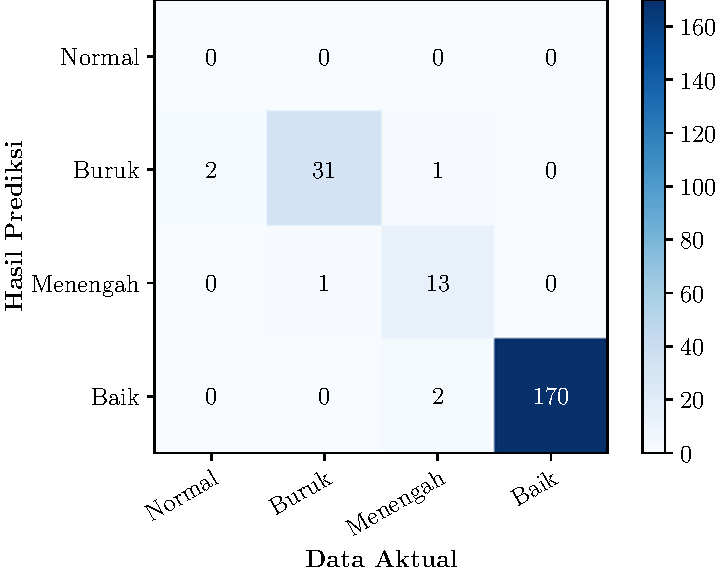
\includegraphics[width=0.6\textwidth]{BAB-4/plot/CM_2_layer_data_besar.pdf}	
			\captionof{figure}{Studi Kasus 1: \textit{Confusion Matrix} LSTM dengan 2 \textit{Hidden Layer}}
			\label{gambar:CM 2 layer DS-1}
%		\end{center}
	\end{minipage}
}

\textit{Confusion matrix} pada Gambar \ref{gambar:CM 2 layer DS-1} memperlihatkan bahwa model sangat baik dalam mendiagnosis indeks kesehatan transformator daya untuk kondisi "Baik" dan sebaliknya untuk kategori kondisi transformator daya "Normal" model sama sekali belum bisa mendiagnosis kelas tersebut. Secara keseluruhan nilai presisi dan sensitifitas dari model dengan menggunakan 2 \textit{hidden layer} dapat dilihat pada Gambar \ref{gambar:presisi sensitivity 2 layer data besar}.

\centerline{\begin{minipage}{\linewidth}
		\centering
		\vspace{12 pt}
		%% Creator: Matplotlib, PGF backend
%%
%% To include the figure in your LaTeX document, write
%%   \input{<filename>.pgf}
%%
%% Make sure the required packages are loaded in your preamble
%%   \usepackage{pgf}
%%
%% Figures using additional raster images can only be included by \input if
%% they are in the same directory as the main LaTeX file. For loading figures
%% from other directories you can use the `import` package
%%   \usepackage{import}
%%
%% and then include the figures with
%%   \import{<path to file>}{<filename>.pgf}
%%
%% Matplotlib used the following preamble
%%
\begingroup%
\makeatletter%
\begin{pgfpicture}%
\pgfpathrectangle{\pgfpointorigin}{\pgfqpoint{5.640000in}{3.140000in}}%
\pgfusepath{use as bounding box, clip}%
\begin{pgfscope}%
\pgfsetbuttcap%
\pgfsetmiterjoin%
\pgfsetlinewidth{0.000000pt}%
\definecolor{currentstroke}{rgb}{1.000000,1.000000,1.000000}%
\pgfsetstrokecolor{currentstroke}%
\pgfsetstrokeopacity{0.000000}%
\pgfsetdash{}{0pt}%
\pgfpathmoveto{\pgfqpoint{0.000000in}{0.000000in}}%
\pgfpathlineto{\pgfqpoint{5.640000in}{0.000000in}}%
\pgfpathlineto{\pgfqpoint{5.640000in}{3.140000in}}%
\pgfpathlineto{\pgfqpoint{0.000000in}{3.140000in}}%
\pgfpathclose%
\pgfusepath{}%
\end{pgfscope}%
\begin{pgfscope}%
\pgfsetbuttcap%
\pgfsetmiterjoin%
\definecolor{currentfill}{rgb}{1.000000,1.000000,1.000000}%
\pgfsetfillcolor{currentfill}%
\pgfsetlinewidth{0.000000pt}%
\definecolor{currentstroke}{rgb}{0.000000,0.000000,0.000000}%
\pgfsetstrokecolor{currentstroke}%
\pgfsetstrokeopacity{0.000000}%
\pgfsetdash{}{0pt}%
\pgfpathmoveto{\pgfqpoint{0.453704in}{0.693723in}}%
\pgfpathlineto{\pgfqpoint{2.730000in}{0.693723in}}%
\pgfpathlineto{\pgfqpoint{2.730000in}{3.140000in}}%
\pgfpathlineto{\pgfqpoint{0.453704in}{3.140000in}}%
\pgfpathclose%
\pgfusepath{fill}%
\end{pgfscope}%
\begin{pgfscope}%
\pgfpathrectangle{\pgfqpoint{0.453704in}{0.693723in}}{\pgfqpoint{2.276296in}{2.446277in}}%
\pgfusepath{clip}%
\pgfsetbuttcap%
\pgfsetmiterjoin%
\definecolor{currentfill}{rgb}{0.121569,0.466667,0.705882}%
\pgfsetfillcolor{currentfill}%
\pgfsetlinewidth{0.000000pt}%
\definecolor{currentstroke}{rgb}{0.000000,0.000000,0.000000}%
\pgfsetstrokecolor{currentstroke}%
\pgfsetstrokeopacity{0.000000}%
\pgfsetdash{}{0pt}%
\pgfpathmoveto{\pgfqpoint{0.557172in}{0.693723in}}%
\pgfpathlineto{\pgfqpoint{0.800626in}{0.693723in}}%
\pgfpathlineto{\pgfqpoint{0.800626in}{0.693723in}}%
\pgfpathlineto{\pgfqpoint{0.557172in}{0.693723in}}%
\pgfpathclose%
\pgfusepath{fill}%
\end{pgfscope}%
\begin{pgfscope}%
\pgfpathrectangle{\pgfqpoint{0.453704in}{0.693723in}}{\pgfqpoint{2.276296in}{2.446277in}}%
\pgfusepath{clip}%
\pgfsetbuttcap%
\pgfsetmiterjoin%
\definecolor{currentfill}{rgb}{0.121569,0.466667,0.705882}%
\pgfsetfillcolor{currentfill}%
\pgfsetlinewidth{0.000000pt}%
\definecolor{currentstroke}{rgb}{0.000000,0.000000,0.000000}%
\pgfsetstrokecolor{currentstroke}%
\pgfsetstrokeopacity{0.000000}%
\pgfsetdash{}{0pt}%
\pgfpathmoveto{\pgfqpoint{1.165807in}{0.693723in}}%
\pgfpathlineto{\pgfqpoint{1.409262in}{0.693723in}}%
\pgfpathlineto{\pgfqpoint{1.409262in}{2.721909in}}%
\pgfpathlineto{\pgfqpoint{1.165807in}{2.721909in}}%
\pgfpathclose%
\pgfusepath{fill}%
\end{pgfscope}%
\begin{pgfscope}%
\pgfpathrectangle{\pgfqpoint{0.453704in}{0.693723in}}{\pgfqpoint{2.276296in}{2.446277in}}%
\pgfusepath{clip}%
\pgfsetbuttcap%
\pgfsetmiterjoin%
\definecolor{currentfill}{rgb}{0.121569,0.466667,0.705882}%
\pgfsetfillcolor{currentfill}%
\pgfsetlinewidth{0.000000pt}%
\definecolor{currentstroke}{rgb}{0.000000,0.000000,0.000000}%
\pgfsetstrokecolor{currentstroke}%
\pgfsetstrokeopacity{0.000000}%
\pgfsetdash{}{0pt}%
\pgfpathmoveto{\pgfqpoint{1.774443in}{0.693723in}}%
\pgfpathlineto{\pgfqpoint{2.017897in}{0.693723in}}%
\pgfpathlineto{\pgfqpoint{2.017897in}{2.759715in}}%
\pgfpathlineto{\pgfqpoint{1.774443in}{2.759715in}}%
\pgfpathclose%
\pgfusepath{fill}%
\end{pgfscope}%
\begin{pgfscope}%
\pgfpathrectangle{\pgfqpoint{0.453704in}{0.693723in}}{\pgfqpoint{2.276296in}{2.446277in}}%
\pgfusepath{clip}%
\pgfsetbuttcap%
\pgfsetmiterjoin%
\definecolor{currentfill}{rgb}{0.121569,0.466667,0.705882}%
\pgfsetfillcolor{currentfill}%
\pgfsetlinewidth{0.000000pt}%
\definecolor{currentstroke}{rgb}{0.000000,0.000000,0.000000}%
\pgfsetstrokecolor{currentstroke}%
\pgfsetstrokeopacity{0.000000}%
\pgfsetdash{}{0pt}%
\pgfpathmoveto{\pgfqpoint{2.383078in}{0.693723in}}%
\pgfpathlineto{\pgfqpoint{2.626532in}{0.693723in}}%
\pgfpathlineto{\pgfqpoint{2.626532in}{2.890924in}}%
\pgfpathlineto{\pgfqpoint{2.383078in}{2.890924in}}%
\pgfpathclose%
\pgfusepath{fill}%
\end{pgfscope}%
\begin{pgfscope}%
\pgfsetbuttcap%
\pgfsetroundjoin%
\definecolor{currentfill}{rgb}{0.000000,0.000000,0.000000}%
\pgfsetfillcolor{currentfill}%
\pgfsetlinewidth{0.803000pt}%
\definecolor{currentstroke}{rgb}{0.000000,0.000000,0.000000}%
\pgfsetstrokecolor{currentstroke}%
\pgfsetdash{}{0pt}%
\pgfsys@defobject{currentmarker}{\pgfqpoint{0.000000in}{-0.048611in}}{\pgfqpoint{0.000000in}{0.000000in}}{%
\pgfpathmoveto{\pgfqpoint{0.000000in}{0.000000in}}%
\pgfpathlineto{\pgfqpoint{0.000000in}{-0.048611in}}%
\pgfusepath{stroke,fill}%
}%
\begin{pgfscope}%
\pgfsys@transformshift{0.678899in}{0.693723in}%
\pgfsys@useobject{currentmarker}{}%
\end{pgfscope}%
\end{pgfscope}%
\begin{pgfscope}%
\definecolor{textcolor}{rgb}{0.000000,0.000000,0.000000}%
\pgfsetstrokecolor{textcolor}%
\pgfsetfillcolor{textcolor}%
\pgftext[x=0.678899in,y=0.596500in,right,top,rotate=30.000000]{\color{textcolor}\rmfamily\fontsize{10.000000}{12.000000}\selectfont Normal}%
\end{pgfscope}%
\begin{pgfscope}%
\pgfsetbuttcap%
\pgfsetroundjoin%
\definecolor{currentfill}{rgb}{0.000000,0.000000,0.000000}%
\pgfsetfillcolor{currentfill}%
\pgfsetlinewidth{0.803000pt}%
\definecolor{currentstroke}{rgb}{0.000000,0.000000,0.000000}%
\pgfsetstrokecolor{currentstroke}%
\pgfsetdash{}{0pt}%
\pgfsys@defobject{currentmarker}{\pgfqpoint{0.000000in}{-0.048611in}}{\pgfqpoint{0.000000in}{0.000000in}}{%
\pgfpathmoveto{\pgfqpoint{0.000000in}{0.000000in}}%
\pgfpathlineto{\pgfqpoint{0.000000in}{-0.048611in}}%
\pgfusepath{stroke,fill}%
}%
\begin{pgfscope}%
\pgfsys@transformshift{1.287534in}{0.693723in}%
\pgfsys@useobject{currentmarker}{}%
\end{pgfscope}%
\end{pgfscope}%
\begin{pgfscope}%
\definecolor{textcolor}{rgb}{0.000000,0.000000,0.000000}%
\pgfsetstrokecolor{textcolor}%
\pgfsetfillcolor{textcolor}%
\pgftext[x=1.287534in,y=0.596500in,right,top,rotate=30.000000]{\color{textcolor}\rmfamily\fontsize{10.000000}{12.000000}\selectfont Buruk}%
\end{pgfscope}%
\begin{pgfscope}%
\pgfsetbuttcap%
\pgfsetroundjoin%
\definecolor{currentfill}{rgb}{0.000000,0.000000,0.000000}%
\pgfsetfillcolor{currentfill}%
\pgfsetlinewidth{0.803000pt}%
\definecolor{currentstroke}{rgb}{0.000000,0.000000,0.000000}%
\pgfsetstrokecolor{currentstroke}%
\pgfsetdash{}{0pt}%
\pgfsys@defobject{currentmarker}{\pgfqpoint{0.000000in}{-0.048611in}}{\pgfqpoint{0.000000in}{0.000000in}}{%
\pgfpathmoveto{\pgfqpoint{0.000000in}{0.000000in}}%
\pgfpathlineto{\pgfqpoint{0.000000in}{-0.048611in}}%
\pgfusepath{stroke,fill}%
}%
\begin{pgfscope}%
\pgfsys@transformshift{1.896170in}{0.693723in}%
\pgfsys@useobject{currentmarker}{}%
\end{pgfscope}%
\end{pgfscope}%
\begin{pgfscope}%
\definecolor{textcolor}{rgb}{0.000000,0.000000,0.000000}%
\pgfsetstrokecolor{textcolor}%
\pgfsetfillcolor{textcolor}%
\pgftext[x=1.896170in,y=0.596500in,right,top,rotate=30.000000]{\color{textcolor}\rmfamily\fontsize{10.000000}{12.000000}\selectfont Menengah}%
\end{pgfscope}%
\begin{pgfscope}%
\pgfsetbuttcap%
\pgfsetroundjoin%
\definecolor{currentfill}{rgb}{0.000000,0.000000,0.000000}%
\pgfsetfillcolor{currentfill}%
\pgfsetlinewidth{0.803000pt}%
\definecolor{currentstroke}{rgb}{0.000000,0.000000,0.000000}%
\pgfsetstrokecolor{currentstroke}%
\pgfsetdash{}{0pt}%
\pgfsys@defobject{currentmarker}{\pgfqpoint{0.000000in}{-0.048611in}}{\pgfqpoint{0.000000in}{0.000000in}}{%
\pgfpathmoveto{\pgfqpoint{0.000000in}{0.000000in}}%
\pgfpathlineto{\pgfqpoint{0.000000in}{-0.048611in}}%
\pgfusepath{stroke,fill}%
}%
\begin{pgfscope}%
\pgfsys@transformshift{2.504805in}{0.693723in}%
\pgfsys@useobject{currentmarker}{}%
\end{pgfscope}%
\end{pgfscope}%
\begin{pgfscope}%
\definecolor{textcolor}{rgb}{0.000000,0.000000,0.000000}%
\pgfsetstrokecolor{textcolor}%
\pgfsetfillcolor{textcolor}%
\pgftext[x=2.504805in,y=0.596500in,right,top,rotate=30.000000]{\color{textcolor}\rmfamily\fontsize{10.000000}{12.000000}\selectfont Baik}%
\end{pgfscope}%
\begin{pgfscope}%
\definecolor{textcolor}{rgb}{0.000000,0.000000,0.000000}%
\pgfsetstrokecolor{textcolor}%
\pgfsetfillcolor{textcolor}%
\pgftext[x=1.591852in,y=0.123457in,,top]{\color{textcolor}\rmfamily\fontsize{10.000000}{12.000000}\selectfont Kategori}%
\end{pgfscope}%
\begin{pgfscope}%
\pgfsetbuttcap%
\pgfsetroundjoin%
\definecolor{currentfill}{rgb}{0.000000,0.000000,0.000000}%
\pgfsetfillcolor{currentfill}%
\pgfsetlinewidth{0.803000pt}%
\definecolor{currentstroke}{rgb}{0.000000,0.000000,0.000000}%
\pgfsetstrokecolor{currentstroke}%
\pgfsetdash{}{0pt}%
\pgfsys@defobject{currentmarker}{\pgfqpoint{-0.048611in}{0.000000in}}{\pgfqpoint{-0.000000in}{0.000000in}}{%
\pgfpathmoveto{\pgfqpoint{-0.000000in}{0.000000in}}%
\pgfpathlineto{\pgfqpoint{-0.048611in}{0.000000in}}%
\pgfusepath{stroke,fill}%
}%
\begin{pgfscope}%
\pgfsys@transformshift{0.453704in}{0.693723in}%
\pgfsys@useobject{currentmarker}{}%
\end{pgfscope}%
\end{pgfscope}%
\begin{pgfscope}%
\definecolor{textcolor}{rgb}{0.000000,0.000000,0.000000}%
\pgfsetstrokecolor{textcolor}%
\pgfsetfillcolor{textcolor}%
\pgftext[x=0.179012in, y=0.645497in, left, base]{\color{textcolor}\rmfamily\fontsize{10.000000}{12.000000}\selectfont \(\displaystyle {0.0}\)}%
\end{pgfscope}%
\begin{pgfscope}%
\pgfsetbuttcap%
\pgfsetroundjoin%
\definecolor{currentfill}{rgb}{0.000000,0.000000,0.000000}%
\pgfsetfillcolor{currentfill}%
\pgfsetlinewidth{0.803000pt}%
\definecolor{currentstroke}{rgb}{0.000000,0.000000,0.000000}%
\pgfsetstrokecolor{currentstroke}%
\pgfsetdash{}{0pt}%
\pgfsys@defobject{currentmarker}{\pgfqpoint{-0.048611in}{0.000000in}}{\pgfqpoint{-0.000000in}{0.000000in}}{%
\pgfpathmoveto{\pgfqpoint{-0.000000in}{0.000000in}}%
\pgfpathlineto{\pgfqpoint{-0.048611in}{0.000000in}}%
\pgfusepath{stroke,fill}%
}%
\begin{pgfscope}%
\pgfsys@transformshift{0.453704in}{1.138500in}%
\pgfsys@useobject{currentmarker}{}%
\end{pgfscope}%
\end{pgfscope}%
\begin{pgfscope}%
\definecolor{textcolor}{rgb}{0.000000,0.000000,0.000000}%
\pgfsetstrokecolor{textcolor}%
\pgfsetfillcolor{textcolor}%
\pgftext[x=0.179012in, y=1.090275in, left, base]{\color{textcolor}\rmfamily\fontsize{10.000000}{12.000000}\selectfont \(\displaystyle {0.2}\)}%
\end{pgfscope}%
\begin{pgfscope}%
\pgfsetbuttcap%
\pgfsetroundjoin%
\definecolor{currentfill}{rgb}{0.000000,0.000000,0.000000}%
\pgfsetfillcolor{currentfill}%
\pgfsetlinewidth{0.803000pt}%
\definecolor{currentstroke}{rgb}{0.000000,0.000000,0.000000}%
\pgfsetstrokecolor{currentstroke}%
\pgfsetdash{}{0pt}%
\pgfsys@defobject{currentmarker}{\pgfqpoint{-0.048611in}{0.000000in}}{\pgfqpoint{-0.000000in}{0.000000in}}{%
\pgfpathmoveto{\pgfqpoint{-0.000000in}{0.000000in}}%
\pgfpathlineto{\pgfqpoint{-0.048611in}{0.000000in}}%
\pgfusepath{stroke,fill}%
}%
\begin{pgfscope}%
\pgfsys@transformshift{0.453704in}{1.583278in}%
\pgfsys@useobject{currentmarker}{}%
\end{pgfscope}%
\end{pgfscope}%
\begin{pgfscope}%
\definecolor{textcolor}{rgb}{0.000000,0.000000,0.000000}%
\pgfsetstrokecolor{textcolor}%
\pgfsetfillcolor{textcolor}%
\pgftext[x=0.179012in, y=1.535053in, left, base]{\color{textcolor}\rmfamily\fontsize{10.000000}{12.000000}\selectfont \(\displaystyle {0.4}\)}%
\end{pgfscope}%
\begin{pgfscope}%
\pgfsetbuttcap%
\pgfsetroundjoin%
\definecolor{currentfill}{rgb}{0.000000,0.000000,0.000000}%
\pgfsetfillcolor{currentfill}%
\pgfsetlinewidth{0.803000pt}%
\definecolor{currentstroke}{rgb}{0.000000,0.000000,0.000000}%
\pgfsetstrokecolor{currentstroke}%
\pgfsetdash{}{0pt}%
\pgfsys@defobject{currentmarker}{\pgfqpoint{-0.048611in}{0.000000in}}{\pgfqpoint{-0.000000in}{0.000000in}}{%
\pgfpathmoveto{\pgfqpoint{-0.000000in}{0.000000in}}%
\pgfpathlineto{\pgfqpoint{-0.048611in}{0.000000in}}%
\pgfusepath{stroke,fill}%
}%
\begin{pgfscope}%
\pgfsys@transformshift{0.453704in}{2.028056in}%
\pgfsys@useobject{currentmarker}{}%
\end{pgfscope}%
\end{pgfscope}%
\begin{pgfscope}%
\definecolor{textcolor}{rgb}{0.000000,0.000000,0.000000}%
\pgfsetstrokecolor{textcolor}%
\pgfsetfillcolor{textcolor}%
\pgftext[x=0.179012in, y=1.979831in, left, base]{\color{textcolor}\rmfamily\fontsize{10.000000}{12.000000}\selectfont \(\displaystyle {0.6}\)}%
\end{pgfscope}%
\begin{pgfscope}%
\pgfsetbuttcap%
\pgfsetroundjoin%
\definecolor{currentfill}{rgb}{0.000000,0.000000,0.000000}%
\pgfsetfillcolor{currentfill}%
\pgfsetlinewidth{0.803000pt}%
\definecolor{currentstroke}{rgb}{0.000000,0.000000,0.000000}%
\pgfsetstrokecolor{currentstroke}%
\pgfsetdash{}{0pt}%
\pgfsys@defobject{currentmarker}{\pgfqpoint{-0.048611in}{0.000000in}}{\pgfqpoint{-0.000000in}{0.000000in}}{%
\pgfpathmoveto{\pgfqpoint{-0.000000in}{0.000000in}}%
\pgfpathlineto{\pgfqpoint{-0.048611in}{0.000000in}}%
\pgfusepath{stroke,fill}%
}%
\begin{pgfscope}%
\pgfsys@transformshift{0.453704in}{2.472833in}%
\pgfsys@useobject{currentmarker}{}%
\end{pgfscope}%
\end{pgfscope}%
\begin{pgfscope}%
\definecolor{textcolor}{rgb}{0.000000,0.000000,0.000000}%
\pgfsetstrokecolor{textcolor}%
\pgfsetfillcolor{textcolor}%
\pgftext[x=0.179012in, y=2.424608in, left, base]{\color{textcolor}\rmfamily\fontsize{10.000000}{12.000000}\selectfont \(\displaystyle {0.8}\)}%
\end{pgfscope}%
\begin{pgfscope}%
\pgfsetbuttcap%
\pgfsetroundjoin%
\definecolor{currentfill}{rgb}{0.000000,0.000000,0.000000}%
\pgfsetfillcolor{currentfill}%
\pgfsetlinewidth{0.803000pt}%
\definecolor{currentstroke}{rgb}{0.000000,0.000000,0.000000}%
\pgfsetstrokecolor{currentstroke}%
\pgfsetdash{}{0pt}%
\pgfsys@defobject{currentmarker}{\pgfqpoint{-0.048611in}{0.000000in}}{\pgfqpoint{-0.000000in}{0.000000in}}{%
\pgfpathmoveto{\pgfqpoint{-0.000000in}{0.000000in}}%
\pgfpathlineto{\pgfqpoint{-0.048611in}{0.000000in}}%
\pgfusepath{stroke,fill}%
}%
\begin{pgfscope}%
\pgfsys@transformshift{0.453704in}{2.917611in}%
\pgfsys@useobject{currentmarker}{}%
\end{pgfscope}%
\end{pgfscope}%
\begin{pgfscope}%
\definecolor{textcolor}{rgb}{0.000000,0.000000,0.000000}%
\pgfsetstrokecolor{textcolor}%
\pgfsetfillcolor{textcolor}%
\pgftext[x=0.179012in, y=2.869386in, left, base]{\color{textcolor}\rmfamily\fontsize{10.000000}{12.000000}\selectfont \(\displaystyle {1.0}\)}%
\end{pgfscope}%
\begin{pgfscope}%
\definecolor{textcolor}{rgb}{0.000000,0.000000,0.000000}%
\pgfsetstrokecolor{textcolor}%
\pgfsetfillcolor{textcolor}%
\pgftext[x=0.123457in,y=1.916861in,,bottom,rotate=90.000000]{\color{textcolor}\rmfamily\fontsize{10.000000}{12.000000}\selectfont Presisi}%
\end{pgfscope}%
\begin{pgfscope}%
\pgfsetrectcap%
\pgfsetmiterjoin%
\pgfsetlinewidth{0.803000pt}%
\definecolor{currentstroke}{rgb}{0.000000,0.000000,0.000000}%
\pgfsetstrokecolor{currentstroke}%
\pgfsetdash{}{0pt}%
\pgfpathmoveto{\pgfqpoint{0.453704in}{0.693723in}}%
\pgfpathlineto{\pgfqpoint{0.453704in}{3.140000in}}%
\pgfusepath{stroke}%
\end{pgfscope}%
\begin{pgfscope}%
\pgfsetrectcap%
\pgfsetmiterjoin%
\pgfsetlinewidth{0.803000pt}%
\definecolor{currentstroke}{rgb}{0.000000,0.000000,0.000000}%
\pgfsetstrokecolor{currentstroke}%
\pgfsetdash{}{0pt}%
\pgfpathmoveto{\pgfqpoint{2.730000in}{0.693723in}}%
\pgfpathlineto{\pgfqpoint{2.730000in}{3.140000in}}%
\pgfusepath{stroke}%
\end{pgfscope}%
\begin{pgfscope}%
\pgfsetrectcap%
\pgfsetmiterjoin%
\pgfsetlinewidth{0.803000pt}%
\definecolor{currentstroke}{rgb}{0.000000,0.000000,0.000000}%
\pgfsetstrokecolor{currentstroke}%
\pgfsetdash{}{0pt}%
\pgfpathmoveto{\pgfqpoint{0.453704in}{0.693723in}}%
\pgfpathlineto{\pgfqpoint{2.730000in}{0.693723in}}%
\pgfusepath{stroke}%
\end{pgfscope}%
\begin{pgfscope}%
\pgfsetrectcap%
\pgfsetmiterjoin%
\pgfsetlinewidth{0.803000pt}%
\definecolor{currentstroke}{rgb}{0.000000,0.000000,0.000000}%
\pgfsetstrokecolor{currentstroke}%
\pgfsetdash{}{0pt}%
\pgfpathmoveto{\pgfqpoint{0.453704in}{3.140000in}}%
\pgfpathlineto{\pgfqpoint{2.730000in}{3.140000in}}%
\pgfusepath{stroke}%
\end{pgfscope}%
\begin{pgfscope}%
\definecolor{textcolor}{rgb}{0.000000,0.000000,0.000000}%
\pgfsetstrokecolor{textcolor}%
\pgfsetfillcolor{textcolor}%
\pgftext[x=0.678899in,y=0.715962in,,bottom]{\color{textcolor}\rmfamily\fontsize{9.000000}{10.800000}\selectfont 0.0}%
\end{pgfscope}%
\begin{pgfscope}%
\definecolor{textcolor}{rgb}{0.000000,0.000000,0.000000}%
\pgfsetstrokecolor{textcolor}%
\pgfsetfillcolor{textcolor}%
\pgftext[x=1.287534in,y=2.744148in,,bottom]{\color{textcolor}\rmfamily\fontsize{9.000000}{10.800000}\selectfont 0.912}%
\end{pgfscope}%
\begin{pgfscope}%
\definecolor{textcolor}{rgb}{0.000000,0.000000,0.000000}%
\pgfsetstrokecolor{textcolor}%
\pgfsetfillcolor{textcolor}%
\pgftext[x=1.896170in,y=2.781954in,,bottom]{\color{textcolor}\rmfamily\fontsize{9.000000}{10.800000}\selectfont 0.929}%
\end{pgfscope}%
\begin{pgfscope}%
\definecolor{textcolor}{rgb}{0.000000,0.000000,0.000000}%
\pgfsetstrokecolor{textcolor}%
\pgfsetfillcolor{textcolor}%
\pgftext[x=2.504805in,y=2.913163in,,bottom]{\color{textcolor}\rmfamily\fontsize{9.000000}{10.800000}\selectfont 0.988}%
\end{pgfscope}%
\begin{pgfscope}%
\pgfsetbuttcap%
\pgfsetmiterjoin%
\definecolor{currentfill}{rgb}{1.000000,1.000000,1.000000}%
\pgfsetfillcolor{currentfill}%
\pgfsetlinewidth{0.000000pt}%
\definecolor{currentstroke}{rgb}{0.000000,0.000000,0.000000}%
\pgfsetstrokecolor{currentstroke}%
\pgfsetstrokeopacity{0.000000}%
\pgfsetdash{}{0pt}%
\pgfpathmoveto{\pgfqpoint{3.363704in}{0.693723in}}%
\pgfpathlineto{\pgfqpoint{5.640000in}{0.693723in}}%
\pgfpathlineto{\pgfqpoint{5.640000in}{3.140000in}}%
\pgfpathlineto{\pgfqpoint{3.363704in}{3.140000in}}%
\pgfpathclose%
\pgfusepath{fill}%
\end{pgfscope}%
\begin{pgfscope}%
\pgfpathrectangle{\pgfqpoint{3.363704in}{0.693723in}}{\pgfqpoint{2.276296in}{2.446277in}}%
\pgfusepath{clip}%
\pgfsetbuttcap%
\pgfsetmiterjoin%
\definecolor{currentfill}{rgb}{1.000000,0.498039,0.054902}%
\pgfsetfillcolor{currentfill}%
\pgfsetlinewidth{0.000000pt}%
\definecolor{currentstroke}{rgb}{0.000000,0.000000,0.000000}%
\pgfsetstrokecolor{currentstroke}%
\pgfsetstrokeopacity{0.000000}%
\pgfsetdash{}{0pt}%
\pgfpathmoveto{\pgfqpoint{3.467172in}{0.693723in}}%
\pgfpathlineto{\pgfqpoint{3.710626in}{0.693723in}}%
\pgfpathlineto{\pgfqpoint{3.710626in}{0.693723in}}%
\pgfpathlineto{\pgfqpoint{3.467172in}{0.693723in}}%
\pgfpathclose%
\pgfusepath{fill}%
\end{pgfscope}%
\begin{pgfscope}%
\pgfpathrectangle{\pgfqpoint{3.363704in}{0.693723in}}{\pgfqpoint{2.276296in}{2.446277in}}%
\pgfusepath{clip}%
\pgfsetbuttcap%
\pgfsetmiterjoin%
\definecolor{currentfill}{rgb}{1.000000,0.498039,0.054902}%
\pgfsetfillcolor{currentfill}%
\pgfsetlinewidth{0.000000pt}%
\definecolor{currentstroke}{rgb}{0.000000,0.000000,0.000000}%
\pgfsetstrokecolor{currentstroke}%
\pgfsetstrokeopacity{0.000000}%
\pgfsetdash{}{0pt}%
\pgfpathmoveto{\pgfqpoint{4.075807in}{0.693723in}}%
\pgfpathlineto{\pgfqpoint{4.319262in}{0.693723in}}%
\pgfpathlineto{\pgfqpoint{4.319262in}{2.848671in}}%
\pgfpathlineto{\pgfqpoint{4.075807in}{2.848671in}}%
\pgfpathclose%
\pgfusepath{fill}%
\end{pgfscope}%
\begin{pgfscope}%
\pgfpathrectangle{\pgfqpoint{3.363704in}{0.693723in}}{\pgfqpoint{2.276296in}{2.446277in}}%
\pgfusepath{clip}%
\pgfsetbuttcap%
\pgfsetmiterjoin%
\definecolor{currentfill}{rgb}{1.000000,0.498039,0.054902}%
\pgfsetfillcolor{currentfill}%
\pgfsetlinewidth{0.000000pt}%
\definecolor{currentstroke}{rgb}{0.000000,0.000000,0.000000}%
\pgfsetstrokecolor{currentstroke}%
\pgfsetstrokeopacity{0.000000}%
\pgfsetdash{}{0pt}%
\pgfpathmoveto{\pgfqpoint{4.684443in}{0.693723in}}%
\pgfpathlineto{\pgfqpoint{4.927897in}{0.693723in}}%
\pgfpathlineto{\pgfqpoint{4.927897in}{2.499520in}}%
\pgfpathlineto{\pgfqpoint{4.684443in}{2.499520in}}%
\pgfpathclose%
\pgfusepath{fill}%
\end{pgfscope}%
\begin{pgfscope}%
\pgfpathrectangle{\pgfqpoint{3.363704in}{0.693723in}}{\pgfqpoint{2.276296in}{2.446277in}}%
\pgfusepath{clip}%
\pgfsetbuttcap%
\pgfsetmiterjoin%
\definecolor{currentfill}{rgb}{1.000000,0.498039,0.054902}%
\pgfsetfillcolor{currentfill}%
\pgfsetlinewidth{0.000000pt}%
\definecolor{currentstroke}{rgb}{0.000000,0.000000,0.000000}%
\pgfsetstrokecolor{currentstroke}%
\pgfsetstrokeopacity{0.000000}%
\pgfsetdash{}{0pt}%
\pgfpathmoveto{\pgfqpoint{5.293078in}{0.693723in}}%
\pgfpathlineto{\pgfqpoint{5.536532in}{0.693723in}}%
\pgfpathlineto{\pgfqpoint{5.536532in}{2.917611in}}%
\pgfpathlineto{\pgfqpoint{5.293078in}{2.917611in}}%
\pgfpathclose%
\pgfusepath{fill}%
\end{pgfscope}%
\begin{pgfscope}%
\pgfsetbuttcap%
\pgfsetroundjoin%
\definecolor{currentfill}{rgb}{0.000000,0.000000,0.000000}%
\pgfsetfillcolor{currentfill}%
\pgfsetlinewidth{0.803000pt}%
\definecolor{currentstroke}{rgb}{0.000000,0.000000,0.000000}%
\pgfsetstrokecolor{currentstroke}%
\pgfsetdash{}{0pt}%
\pgfsys@defobject{currentmarker}{\pgfqpoint{0.000000in}{-0.048611in}}{\pgfqpoint{0.000000in}{0.000000in}}{%
\pgfpathmoveto{\pgfqpoint{0.000000in}{0.000000in}}%
\pgfpathlineto{\pgfqpoint{0.000000in}{-0.048611in}}%
\pgfusepath{stroke,fill}%
}%
\begin{pgfscope}%
\pgfsys@transformshift{3.588899in}{0.693723in}%
\pgfsys@useobject{currentmarker}{}%
\end{pgfscope}%
\end{pgfscope}%
\begin{pgfscope}%
\definecolor{textcolor}{rgb}{0.000000,0.000000,0.000000}%
\pgfsetstrokecolor{textcolor}%
\pgfsetfillcolor{textcolor}%
\pgftext[x=3.588899in,y=0.596500in,right,top,rotate=30.000000]{\color{textcolor}\rmfamily\fontsize{10.000000}{12.000000}\selectfont Normal}%
\end{pgfscope}%
\begin{pgfscope}%
\pgfsetbuttcap%
\pgfsetroundjoin%
\definecolor{currentfill}{rgb}{0.000000,0.000000,0.000000}%
\pgfsetfillcolor{currentfill}%
\pgfsetlinewidth{0.803000pt}%
\definecolor{currentstroke}{rgb}{0.000000,0.000000,0.000000}%
\pgfsetstrokecolor{currentstroke}%
\pgfsetdash{}{0pt}%
\pgfsys@defobject{currentmarker}{\pgfqpoint{0.000000in}{-0.048611in}}{\pgfqpoint{0.000000in}{0.000000in}}{%
\pgfpathmoveto{\pgfqpoint{0.000000in}{0.000000in}}%
\pgfpathlineto{\pgfqpoint{0.000000in}{-0.048611in}}%
\pgfusepath{stroke,fill}%
}%
\begin{pgfscope}%
\pgfsys@transformshift{4.197534in}{0.693723in}%
\pgfsys@useobject{currentmarker}{}%
\end{pgfscope}%
\end{pgfscope}%
\begin{pgfscope}%
\definecolor{textcolor}{rgb}{0.000000,0.000000,0.000000}%
\pgfsetstrokecolor{textcolor}%
\pgfsetfillcolor{textcolor}%
\pgftext[x=4.197534in,y=0.596500in,right,top,rotate=30.000000]{\color{textcolor}\rmfamily\fontsize{10.000000}{12.000000}\selectfont Buruk}%
\end{pgfscope}%
\begin{pgfscope}%
\pgfsetbuttcap%
\pgfsetroundjoin%
\definecolor{currentfill}{rgb}{0.000000,0.000000,0.000000}%
\pgfsetfillcolor{currentfill}%
\pgfsetlinewidth{0.803000pt}%
\definecolor{currentstroke}{rgb}{0.000000,0.000000,0.000000}%
\pgfsetstrokecolor{currentstroke}%
\pgfsetdash{}{0pt}%
\pgfsys@defobject{currentmarker}{\pgfqpoint{0.000000in}{-0.048611in}}{\pgfqpoint{0.000000in}{0.000000in}}{%
\pgfpathmoveto{\pgfqpoint{0.000000in}{0.000000in}}%
\pgfpathlineto{\pgfqpoint{0.000000in}{-0.048611in}}%
\pgfusepath{stroke,fill}%
}%
\begin{pgfscope}%
\pgfsys@transformshift{4.806170in}{0.693723in}%
\pgfsys@useobject{currentmarker}{}%
\end{pgfscope}%
\end{pgfscope}%
\begin{pgfscope}%
\definecolor{textcolor}{rgb}{0.000000,0.000000,0.000000}%
\pgfsetstrokecolor{textcolor}%
\pgfsetfillcolor{textcolor}%
\pgftext[x=4.806170in,y=0.596500in,right,top,rotate=30.000000]{\color{textcolor}\rmfamily\fontsize{10.000000}{12.000000}\selectfont Menengah}%
\end{pgfscope}%
\begin{pgfscope}%
\pgfsetbuttcap%
\pgfsetroundjoin%
\definecolor{currentfill}{rgb}{0.000000,0.000000,0.000000}%
\pgfsetfillcolor{currentfill}%
\pgfsetlinewidth{0.803000pt}%
\definecolor{currentstroke}{rgb}{0.000000,0.000000,0.000000}%
\pgfsetstrokecolor{currentstroke}%
\pgfsetdash{}{0pt}%
\pgfsys@defobject{currentmarker}{\pgfqpoint{0.000000in}{-0.048611in}}{\pgfqpoint{0.000000in}{0.000000in}}{%
\pgfpathmoveto{\pgfqpoint{0.000000in}{0.000000in}}%
\pgfpathlineto{\pgfqpoint{0.000000in}{-0.048611in}}%
\pgfusepath{stroke,fill}%
}%
\begin{pgfscope}%
\pgfsys@transformshift{5.414805in}{0.693723in}%
\pgfsys@useobject{currentmarker}{}%
\end{pgfscope}%
\end{pgfscope}%
\begin{pgfscope}%
\definecolor{textcolor}{rgb}{0.000000,0.000000,0.000000}%
\pgfsetstrokecolor{textcolor}%
\pgfsetfillcolor{textcolor}%
\pgftext[x=5.414805in,y=0.596500in,right,top,rotate=30.000000]{\color{textcolor}\rmfamily\fontsize{10.000000}{12.000000}\selectfont Baik}%
\end{pgfscope}%
\begin{pgfscope}%
\definecolor{textcolor}{rgb}{0.000000,0.000000,0.000000}%
\pgfsetstrokecolor{textcolor}%
\pgfsetfillcolor{textcolor}%
\pgftext[x=4.501852in,y=0.123457in,,top]{\color{textcolor}\rmfamily\fontsize{10.000000}{12.000000}\selectfont Kategori}%
\end{pgfscope}%
\begin{pgfscope}%
\pgfsetbuttcap%
\pgfsetroundjoin%
\definecolor{currentfill}{rgb}{0.000000,0.000000,0.000000}%
\pgfsetfillcolor{currentfill}%
\pgfsetlinewidth{0.803000pt}%
\definecolor{currentstroke}{rgb}{0.000000,0.000000,0.000000}%
\pgfsetstrokecolor{currentstroke}%
\pgfsetdash{}{0pt}%
\pgfsys@defobject{currentmarker}{\pgfqpoint{-0.048611in}{0.000000in}}{\pgfqpoint{-0.000000in}{0.000000in}}{%
\pgfpathmoveto{\pgfqpoint{-0.000000in}{0.000000in}}%
\pgfpathlineto{\pgfqpoint{-0.048611in}{0.000000in}}%
\pgfusepath{stroke,fill}%
}%
\begin{pgfscope}%
\pgfsys@transformshift{3.363704in}{0.693723in}%
\pgfsys@useobject{currentmarker}{}%
\end{pgfscope}%
\end{pgfscope}%
\begin{pgfscope}%
\definecolor{textcolor}{rgb}{0.000000,0.000000,0.000000}%
\pgfsetstrokecolor{textcolor}%
\pgfsetfillcolor{textcolor}%
\pgftext[x=3.089012in, y=0.645497in, left, base]{\color{textcolor}\rmfamily\fontsize{10.000000}{12.000000}\selectfont \(\displaystyle {0.0}\)}%
\end{pgfscope}%
\begin{pgfscope}%
\pgfsetbuttcap%
\pgfsetroundjoin%
\definecolor{currentfill}{rgb}{0.000000,0.000000,0.000000}%
\pgfsetfillcolor{currentfill}%
\pgfsetlinewidth{0.803000pt}%
\definecolor{currentstroke}{rgb}{0.000000,0.000000,0.000000}%
\pgfsetstrokecolor{currentstroke}%
\pgfsetdash{}{0pt}%
\pgfsys@defobject{currentmarker}{\pgfqpoint{-0.048611in}{0.000000in}}{\pgfqpoint{-0.000000in}{0.000000in}}{%
\pgfpathmoveto{\pgfqpoint{-0.000000in}{0.000000in}}%
\pgfpathlineto{\pgfqpoint{-0.048611in}{0.000000in}}%
\pgfusepath{stroke,fill}%
}%
\begin{pgfscope}%
\pgfsys@transformshift{3.363704in}{1.138500in}%
\pgfsys@useobject{currentmarker}{}%
\end{pgfscope}%
\end{pgfscope}%
\begin{pgfscope}%
\definecolor{textcolor}{rgb}{0.000000,0.000000,0.000000}%
\pgfsetstrokecolor{textcolor}%
\pgfsetfillcolor{textcolor}%
\pgftext[x=3.089012in, y=1.090275in, left, base]{\color{textcolor}\rmfamily\fontsize{10.000000}{12.000000}\selectfont \(\displaystyle {0.2}\)}%
\end{pgfscope}%
\begin{pgfscope}%
\pgfsetbuttcap%
\pgfsetroundjoin%
\definecolor{currentfill}{rgb}{0.000000,0.000000,0.000000}%
\pgfsetfillcolor{currentfill}%
\pgfsetlinewidth{0.803000pt}%
\definecolor{currentstroke}{rgb}{0.000000,0.000000,0.000000}%
\pgfsetstrokecolor{currentstroke}%
\pgfsetdash{}{0pt}%
\pgfsys@defobject{currentmarker}{\pgfqpoint{-0.048611in}{0.000000in}}{\pgfqpoint{-0.000000in}{0.000000in}}{%
\pgfpathmoveto{\pgfqpoint{-0.000000in}{0.000000in}}%
\pgfpathlineto{\pgfqpoint{-0.048611in}{0.000000in}}%
\pgfusepath{stroke,fill}%
}%
\begin{pgfscope}%
\pgfsys@transformshift{3.363704in}{1.583278in}%
\pgfsys@useobject{currentmarker}{}%
\end{pgfscope}%
\end{pgfscope}%
\begin{pgfscope}%
\definecolor{textcolor}{rgb}{0.000000,0.000000,0.000000}%
\pgfsetstrokecolor{textcolor}%
\pgfsetfillcolor{textcolor}%
\pgftext[x=3.089012in, y=1.535053in, left, base]{\color{textcolor}\rmfamily\fontsize{10.000000}{12.000000}\selectfont \(\displaystyle {0.4}\)}%
\end{pgfscope}%
\begin{pgfscope}%
\pgfsetbuttcap%
\pgfsetroundjoin%
\definecolor{currentfill}{rgb}{0.000000,0.000000,0.000000}%
\pgfsetfillcolor{currentfill}%
\pgfsetlinewidth{0.803000pt}%
\definecolor{currentstroke}{rgb}{0.000000,0.000000,0.000000}%
\pgfsetstrokecolor{currentstroke}%
\pgfsetdash{}{0pt}%
\pgfsys@defobject{currentmarker}{\pgfqpoint{-0.048611in}{0.000000in}}{\pgfqpoint{-0.000000in}{0.000000in}}{%
\pgfpathmoveto{\pgfqpoint{-0.000000in}{0.000000in}}%
\pgfpathlineto{\pgfqpoint{-0.048611in}{0.000000in}}%
\pgfusepath{stroke,fill}%
}%
\begin{pgfscope}%
\pgfsys@transformshift{3.363704in}{2.028056in}%
\pgfsys@useobject{currentmarker}{}%
\end{pgfscope}%
\end{pgfscope}%
\begin{pgfscope}%
\definecolor{textcolor}{rgb}{0.000000,0.000000,0.000000}%
\pgfsetstrokecolor{textcolor}%
\pgfsetfillcolor{textcolor}%
\pgftext[x=3.089012in, y=1.979831in, left, base]{\color{textcolor}\rmfamily\fontsize{10.000000}{12.000000}\selectfont \(\displaystyle {0.6}\)}%
\end{pgfscope}%
\begin{pgfscope}%
\pgfsetbuttcap%
\pgfsetroundjoin%
\definecolor{currentfill}{rgb}{0.000000,0.000000,0.000000}%
\pgfsetfillcolor{currentfill}%
\pgfsetlinewidth{0.803000pt}%
\definecolor{currentstroke}{rgb}{0.000000,0.000000,0.000000}%
\pgfsetstrokecolor{currentstroke}%
\pgfsetdash{}{0pt}%
\pgfsys@defobject{currentmarker}{\pgfqpoint{-0.048611in}{0.000000in}}{\pgfqpoint{-0.000000in}{0.000000in}}{%
\pgfpathmoveto{\pgfqpoint{-0.000000in}{0.000000in}}%
\pgfpathlineto{\pgfqpoint{-0.048611in}{0.000000in}}%
\pgfusepath{stroke,fill}%
}%
\begin{pgfscope}%
\pgfsys@transformshift{3.363704in}{2.472833in}%
\pgfsys@useobject{currentmarker}{}%
\end{pgfscope}%
\end{pgfscope}%
\begin{pgfscope}%
\definecolor{textcolor}{rgb}{0.000000,0.000000,0.000000}%
\pgfsetstrokecolor{textcolor}%
\pgfsetfillcolor{textcolor}%
\pgftext[x=3.089012in, y=2.424608in, left, base]{\color{textcolor}\rmfamily\fontsize{10.000000}{12.000000}\selectfont \(\displaystyle {0.8}\)}%
\end{pgfscope}%
\begin{pgfscope}%
\pgfsetbuttcap%
\pgfsetroundjoin%
\definecolor{currentfill}{rgb}{0.000000,0.000000,0.000000}%
\pgfsetfillcolor{currentfill}%
\pgfsetlinewidth{0.803000pt}%
\definecolor{currentstroke}{rgb}{0.000000,0.000000,0.000000}%
\pgfsetstrokecolor{currentstroke}%
\pgfsetdash{}{0pt}%
\pgfsys@defobject{currentmarker}{\pgfqpoint{-0.048611in}{0.000000in}}{\pgfqpoint{-0.000000in}{0.000000in}}{%
\pgfpathmoveto{\pgfqpoint{-0.000000in}{0.000000in}}%
\pgfpathlineto{\pgfqpoint{-0.048611in}{0.000000in}}%
\pgfusepath{stroke,fill}%
}%
\begin{pgfscope}%
\pgfsys@transformshift{3.363704in}{2.917611in}%
\pgfsys@useobject{currentmarker}{}%
\end{pgfscope}%
\end{pgfscope}%
\begin{pgfscope}%
\definecolor{textcolor}{rgb}{0.000000,0.000000,0.000000}%
\pgfsetstrokecolor{textcolor}%
\pgfsetfillcolor{textcolor}%
\pgftext[x=3.089012in, y=2.869386in, left, base]{\color{textcolor}\rmfamily\fontsize{10.000000}{12.000000}\selectfont \(\displaystyle {1.0}\)}%
\end{pgfscope}%
\begin{pgfscope}%
\definecolor{textcolor}{rgb}{0.000000,0.000000,0.000000}%
\pgfsetstrokecolor{textcolor}%
\pgfsetfillcolor{textcolor}%
\pgftext[x=3.033457in,y=1.916861in,,bottom,rotate=90.000000]{\color{textcolor}\rmfamily\fontsize{10.000000}{12.000000}\selectfont Sensitivitas}%
\end{pgfscope}%
\begin{pgfscope}%
\pgfsetrectcap%
\pgfsetmiterjoin%
\pgfsetlinewidth{0.803000pt}%
\definecolor{currentstroke}{rgb}{0.000000,0.000000,0.000000}%
\pgfsetstrokecolor{currentstroke}%
\pgfsetdash{}{0pt}%
\pgfpathmoveto{\pgfqpoint{3.363704in}{0.693723in}}%
\pgfpathlineto{\pgfqpoint{3.363704in}{3.140000in}}%
\pgfusepath{stroke}%
\end{pgfscope}%
\begin{pgfscope}%
\pgfsetrectcap%
\pgfsetmiterjoin%
\pgfsetlinewidth{0.803000pt}%
\definecolor{currentstroke}{rgb}{0.000000,0.000000,0.000000}%
\pgfsetstrokecolor{currentstroke}%
\pgfsetdash{}{0pt}%
\pgfpathmoveto{\pgfqpoint{5.640000in}{0.693723in}}%
\pgfpathlineto{\pgfqpoint{5.640000in}{3.140000in}}%
\pgfusepath{stroke}%
\end{pgfscope}%
\begin{pgfscope}%
\pgfsetrectcap%
\pgfsetmiterjoin%
\pgfsetlinewidth{0.803000pt}%
\definecolor{currentstroke}{rgb}{0.000000,0.000000,0.000000}%
\pgfsetstrokecolor{currentstroke}%
\pgfsetdash{}{0pt}%
\pgfpathmoveto{\pgfqpoint{3.363704in}{0.693723in}}%
\pgfpathlineto{\pgfqpoint{5.640000in}{0.693723in}}%
\pgfusepath{stroke}%
\end{pgfscope}%
\begin{pgfscope}%
\pgfsetrectcap%
\pgfsetmiterjoin%
\pgfsetlinewidth{0.803000pt}%
\definecolor{currentstroke}{rgb}{0.000000,0.000000,0.000000}%
\pgfsetstrokecolor{currentstroke}%
\pgfsetdash{}{0pt}%
\pgfpathmoveto{\pgfqpoint{3.363704in}{3.140000in}}%
\pgfpathlineto{\pgfqpoint{5.640000in}{3.140000in}}%
\pgfusepath{stroke}%
\end{pgfscope}%
\begin{pgfscope}%
\definecolor{textcolor}{rgb}{0.000000,0.000000,0.000000}%
\pgfsetstrokecolor{textcolor}%
\pgfsetfillcolor{textcolor}%
\pgftext[x=3.588899in,y=0.715962in,,bottom]{\color{textcolor}\rmfamily\fontsize{9.000000}{10.800000}\selectfont 0.0}%
\end{pgfscope}%
\begin{pgfscope}%
\definecolor{textcolor}{rgb}{0.000000,0.000000,0.000000}%
\pgfsetstrokecolor{textcolor}%
\pgfsetfillcolor{textcolor}%
\pgftext[x=4.197534in,y=2.870909in,,bottom]{\color{textcolor}\rmfamily\fontsize{9.000000}{10.800000}\selectfont 0.969}%
\end{pgfscope}%
\begin{pgfscope}%
\definecolor{textcolor}{rgb}{0.000000,0.000000,0.000000}%
\pgfsetstrokecolor{textcolor}%
\pgfsetfillcolor{textcolor}%
\pgftext[x=4.806170in,y=2.521759in,,bottom]{\color{textcolor}\rmfamily\fontsize{9.000000}{10.800000}\selectfont 0.812}%
\end{pgfscope}%
\begin{pgfscope}%
\definecolor{textcolor}{rgb}{0.000000,0.000000,0.000000}%
\pgfsetstrokecolor{textcolor}%
\pgfsetfillcolor{textcolor}%
\pgftext[x=5.414805in,y=2.939850in,,bottom]{\color{textcolor}\rmfamily\fontsize{9.000000}{10.800000}\selectfont 1.0}%
\end{pgfscope}%
\end{pgfpicture}%
\makeatother%
\endgroup%

		\captionof{figure}{Studi Kasus 1: Presisi Percobaan Perubahan Layer}
		\label{gambar:presisi sensitivity 2 layer data besar}
\end{minipage}}

Berdasarkan Gambar \ref{gambar:presisi sensitivity 2 layer data besar} dapat diketahui secara mudah bahwa pada model memiliki sensitivitas yang tinggi untuk mendiagnosis kondisi transformator daya "Baik", namun karena terlampau sensitif mengakibatkan indeks kesehatan transformator daya yang seharusnya terdiagnosis sebagai kondisi "Menengah" menjadi terprediksi sebagai "Baik". Jika dilihat dari segi presisi untuk kategori indeks kesehatan "Buruk", "Menengah", dan "Baik" memiliki presisi yang di atas 90\%. Namun untuk kategori "Normal" baik pada presisi maupun sensitivitas keduanya masih memiliki nilai yang buruk. Dengan melihat hasil perolehan performa model LSTM menggunakan 2 \textit{hidden layer}, maka perlu dilakukan percobaan lanjutan dengan model LSTM 2 \textit{hidden layer} untuk memperbaiki dari presisi dan sensitivitas dari kategori "Normal" pada hasil diagnosis.\par



\subsection{Perubahan Fungsi Aktivasi}
Pada percobaan pengaturan \textit{hyperparameter hidden layer} sebelumnya diketahui dapat menghasilkan hasil akurasi sebesar 97\% secara keseluruhan. Namun, pada model tersebut masih belum bisa mendiagnosis indeks kesehatan transformator daya pada kategori "Normal". Pada percobaan ini akan dilakukan untuk memperbaiki model agar memiliki sensitivitas yang seimbang pada semua kategori indeks kesehatan transformator daya. Percobaan dilakukan dengan melakukan perubahan \textit{hyperparameter} pada fungsi aktivasi yang digunakan. Pada dasarnya model LSTM menggunakan fungsi aktivasi berupa \textit{sigmoid} di beberapa bagian, namun tidak menutup kemungkinan jika perubahan fungsi aktivasi dapat memberikan hasil model yang berbeda. Terdapat beberapa fungsi aktivasi yang akan di uji coba pada percobaan ini diantaranya adalah \textit{tanh, relu, softmax, selu, elu, softplus,} dan \textit{softsign}. Proses percobaan dilakukan dengan pengulangan sebanyak 30 kali untuk setiap penggunaan fungsi aktivasi.


\centerline{
\begin{minipage}{\linewidth}
	\vspace{12 pt}
	\centering
	%% Creator: Matplotlib, PGF backend
%%
%% To include the figure in your LaTeX document, write
%%   \input{<filename>.pgf}
%%
%% Make sure the required packages are loaded in your preamble
%%   \usepackage{pgf}
%%
%% Figures using additional raster images can only be included by \input if
%% they are in the same directory as the main LaTeX file. For loading figures
%% from other directories you can use the `import` package
%%   \usepackage{import}
%%
%% and then include the figures with
%%   \import{<path to file>}{<filename>.pgf}
%%
%% Matplotlib used the following preamble
%%
\begingroup%
\makeatletter%
\begin{pgfpicture}%
\pgfpathrectangle{\pgfpointorigin}{\pgfqpoint{6.000000in}{4.000000in}}%
\pgfusepath{use as bounding box, clip}%
\begin{pgfscope}%
\pgfsetbuttcap%
\pgfsetmiterjoin%
\pgfsetlinewidth{0.000000pt}%
\definecolor{currentstroke}{rgb}{1.000000,1.000000,1.000000}%
\pgfsetstrokecolor{currentstroke}%
\pgfsetstrokeopacity{0.000000}%
\pgfsetdash{}{0pt}%
\pgfpathmoveto{\pgfqpoint{0.000000in}{0.000000in}}%
\pgfpathlineto{\pgfqpoint{6.000000in}{0.000000in}}%
\pgfpathlineto{\pgfqpoint{6.000000in}{4.000000in}}%
\pgfpathlineto{\pgfqpoint{0.000000in}{4.000000in}}%
\pgfpathclose%
\pgfusepath{}%
\end{pgfscope}%
\begin{pgfscope}%
\pgfsetbuttcap%
\pgfsetmiterjoin%
\definecolor{currentfill}{rgb}{1.000000,1.000000,1.000000}%
\pgfsetfillcolor{currentfill}%
\pgfsetlinewidth{0.000000pt}%
\definecolor{currentstroke}{rgb}{0.000000,0.000000,0.000000}%
\pgfsetstrokecolor{currentstroke}%
\pgfsetstrokeopacity{0.000000}%
\pgfsetdash{}{0pt}%
\pgfpathmoveto{\pgfqpoint{0.750000in}{0.500000in}}%
\pgfpathlineto{\pgfqpoint{5.400000in}{0.500000in}}%
\pgfpathlineto{\pgfqpoint{5.400000in}{3.520000in}}%
\pgfpathlineto{\pgfqpoint{0.750000in}{3.520000in}}%
\pgfpathclose%
\pgfusepath{fill}%
\end{pgfscope}%
\begin{pgfscope}%
\pgfpathrectangle{\pgfqpoint{0.750000in}{0.500000in}}{\pgfqpoint{4.650000in}{3.020000in}}%
\pgfusepath{clip}%
\pgfsetbuttcap%
\pgfsetmiterjoin%
\definecolor{currentfill}{rgb}{0.121569,0.466667,0.705882}%
\pgfsetfillcolor{currentfill}%
\pgfsetlinewidth{0.000000pt}%
\definecolor{currentstroke}{rgb}{0.000000,0.000000,0.000000}%
\pgfsetstrokecolor{currentstroke}%
\pgfsetstrokeopacity{0.000000}%
\pgfsetdash{}{0pt}%
\pgfpathmoveto{\pgfqpoint{0.961364in}{-14.600000in}}%
\pgfpathlineto{\pgfqpoint{1.128230in}{-14.600000in}}%
\pgfpathlineto{\pgfqpoint{1.128230in}{2.258706in}}%
\pgfpathlineto{\pgfqpoint{0.961364in}{2.258706in}}%
\pgfpathclose%
\pgfusepath{fill}%
\end{pgfscope}%
\begin{pgfscope}%
\pgfpathrectangle{\pgfqpoint{0.750000in}{0.500000in}}{\pgfqpoint{4.650000in}{3.020000in}}%
\pgfusepath{clip}%
\pgfsetbuttcap%
\pgfsetmiterjoin%
\definecolor{currentfill}{rgb}{0.121569,0.466667,0.705882}%
\pgfsetfillcolor{currentfill}%
\pgfsetlinewidth{0.000000pt}%
\definecolor{currentstroke}{rgb}{0.000000,0.000000,0.000000}%
\pgfsetstrokecolor{currentstroke}%
\pgfsetstrokeopacity{0.000000}%
\pgfsetdash{}{0pt}%
\pgfpathmoveto{\pgfqpoint{1.517584in}{-14.600000in}}%
\pgfpathlineto{\pgfqpoint{1.684450in}{-14.600000in}}%
\pgfpathlineto{\pgfqpoint{1.684450in}{2.791647in}}%
\pgfpathlineto{\pgfqpoint{1.517584in}{2.791647in}}%
\pgfpathclose%
\pgfusepath{fill}%
\end{pgfscope}%
\begin{pgfscope}%
\pgfpathrectangle{\pgfqpoint{0.750000in}{0.500000in}}{\pgfqpoint{4.650000in}{3.020000in}}%
\pgfusepath{clip}%
\pgfsetbuttcap%
\pgfsetmiterjoin%
\definecolor{currentfill}{rgb}{0.121569,0.466667,0.705882}%
\pgfsetfillcolor{currentfill}%
\pgfsetlinewidth{0.000000pt}%
\definecolor{currentstroke}{rgb}{0.000000,0.000000,0.000000}%
\pgfsetstrokecolor{currentstroke}%
\pgfsetstrokeopacity{0.000000}%
\pgfsetdash{}{0pt}%
\pgfpathmoveto{\pgfqpoint{2.073804in}{-14.600000in}}%
\pgfpathlineto{\pgfqpoint{2.240670in}{-14.600000in}}%
\pgfpathlineto{\pgfqpoint{2.240670in}{2.720588in}}%
\pgfpathlineto{\pgfqpoint{2.073804in}{2.720588in}}%
\pgfpathclose%
\pgfusepath{fill}%
\end{pgfscope}%
\begin{pgfscope}%
\pgfpathrectangle{\pgfqpoint{0.750000in}{0.500000in}}{\pgfqpoint{4.650000in}{3.020000in}}%
\pgfusepath{clip}%
\pgfsetbuttcap%
\pgfsetmiterjoin%
\definecolor{currentfill}{rgb}{0.121569,0.466667,0.705882}%
\pgfsetfillcolor{currentfill}%
\pgfsetlinewidth{0.000000pt}%
\definecolor{currentstroke}{rgb}{0.000000,0.000000,0.000000}%
\pgfsetstrokecolor{currentstroke}%
\pgfsetstrokeopacity{0.000000}%
\pgfsetdash{}{0pt}%
\pgfpathmoveto{\pgfqpoint{2.630024in}{-14.600000in}}%
\pgfpathlineto{\pgfqpoint{2.796890in}{-14.600000in}}%
\pgfpathlineto{\pgfqpoint{2.796890in}{1.050706in}}%
\pgfpathlineto{\pgfqpoint{2.630024in}{1.050706in}}%
\pgfpathclose%
\pgfusepath{fill}%
\end{pgfscope}%
\begin{pgfscope}%
\pgfpathrectangle{\pgfqpoint{0.750000in}{0.500000in}}{\pgfqpoint{4.650000in}{3.020000in}}%
\pgfusepath{clip}%
\pgfsetbuttcap%
\pgfsetmiterjoin%
\definecolor{currentfill}{rgb}{0.121569,0.466667,0.705882}%
\pgfsetfillcolor{currentfill}%
\pgfsetlinewidth{0.000000pt}%
\definecolor{currentstroke}{rgb}{0.000000,0.000000,0.000000}%
\pgfsetstrokecolor{currentstroke}%
\pgfsetstrokeopacity{0.000000}%
\pgfsetdash{}{0pt}%
\pgfpathmoveto{\pgfqpoint{3.186244in}{-14.600000in}}%
\pgfpathlineto{\pgfqpoint{3.353110in}{-14.600000in}}%
\pgfpathlineto{\pgfqpoint{3.353110in}{3.022588in}}%
\pgfpathlineto{\pgfqpoint{3.186244in}{3.022588in}}%
\pgfpathclose%
\pgfusepath{fill}%
\end{pgfscope}%
\begin{pgfscope}%
\pgfpathrectangle{\pgfqpoint{0.750000in}{0.500000in}}{\pgfqpoint{4.650000in}{3.020000in}}%
\pgfusepath{clip}%
\pgfsetbuttcap%
\pgfsetmiterjoin%
\definecolor{currentfill}{rgb}{0.121569,0.466667,0.705882}%
\pgfsetfillcolor{currentfill}%
\pgfsetlinewidth{0.000000pt}%
\definecolor{currentstroke}{rgb}{0.000000,0.000000,0.000000}%
\pgfsetstrokecolor{currentstroke}%
\pgfsetstrokeopacity{0.000000}%
\pgfsetdash{}{0pt}%
\pgfpathmoveto{\pgfqpoint{3.742464in}{-14.600000in}}%
\pgfpathlineto{\pgfqpoint{3.909330in}{-14.600000in}}%
\pgfpathlineto{\pgfqpoint{3.909330in}{2.844941in}}%
\pgfpathlineto{\pgfqpoint{3.742464in}{2.844941in}}%
\pgfpathclose%
\pgfusepath{fill}%
\end{pgfscope}%
\begin{pgfscope}%
\pgfpathrectangle{\pgfqpoint{0.750000in}{0.500000in}}{\pgfqpoint{4.650000in}{3.020000in}}%
\pgfusepath{clip}%
\pgfsetbuttcap%
\pgfsetmiterjoin%
\definecolor{currentfill}{rgb}{0.121569,0.466667,0.705882}%
\pgfsetfillcolor{currentfill}%
\pgfsetlinewidth{0.000000pt}%
\definecolor{currentstroke}{rgb}{0.000000,0.000000,0.000000}%
\pgfsetstrokecolor{currentstroke}%
\pgfsetstrokeopacity{0.000000}%
\pgfsetdash{}{0pt}%
\pgfpathmoveto{\pgfqpoint{4.298684in}{-14.600000in}}%
\pgfpathlineto{\pgfqpoint{4.465550in}{-14.600000in}}%
\pgfpathlineto{\pgfqpoint{4.465550in}{2.898235in}}%
\pgfpathlineto{\pgfqpoint{4.298684in}{2.898235in}}%
\pgfpathclose%
\pgfusepath{fill}%
\end{pgfscope}%
\begin{pgfscope}%
\pgfpathrectangle{\pgfqpoint{0.750000in}{0.500000in}}{\pgfqpoint{4.650000in}{3.020000in}}%
\pgfusepath{clip}%
\pgfsetbuttcap%
\pgfsetmiterjoin%
\definecolor{currentfill}{rgb}{0.121569,0.466667,0.705882}%
\pgfsetfillcolor{currentfill}%
\pgfsetlinewidth{0.000000pt}%
\definecolor{currentstroke}{rgb}{0.000000,0.000000,0.000000}%
\pgfsetstrokecolor{currentstroke}%
\pgfsetstrokeopacity{0.000000}%
\pgfsetdash{}{0pt}%
\pgfpathmoveto{\pgfqpoint{4.854904in}{-14.600000in}}%
\pgfpathlineto{\pgfqpoint{5.021770in}{-14.600000in}}%
\pgfpathlineto{\pgfqpoint{5.021770in}{2.685059in}}%
\pgfpathlineto{\pgfqpoint{4.854904in}{2.685059in}}%
\pgfpathclose%
\pgfusepath{fill}%
\end{pgfscope}%
\begin{pgfscope}%
\pgfpathrectangle{\pgfqpoint{0.750000in}{0.500000in}}{\pgfqpoint{4.650000in}{3.020000in}}%
\pgfusepath{clip}%
\pgfsetbuttcap%
\pgfsetmiterjoin%
\definecolor{currentfill}{rgb}{1.000000,0.498039,0.054902}%
\pgfsetfillcolor{currentfill}%
\pgfsetlinewidth{0.000000pt}%
\definecolor{currentstroke}{rgb}{0.000000,0.000000,0.000000}%
\pgfsetstrokecolor{currentstroke}%
\pgfsetstrokeopacity{0.000000}%
\pgfsetdash{}{0pt}%
\pgfpathmoveto{\pgfqpoint{1.128230in}{-14.600000in}}%
\pgfpathlineto{\pgfqpoint{1.295096in}{-14.600000in}}%
\pgfpathlineto{\pgfqpoint{1.295096in}{2.152118in}}%
\pgfpathlineto{\pgfqpoint{1.128230in}{2.152118in}}%
\pgfpathclose%
\pgfusepath{fill}%
\end{pgfscope}%
\begin{pgfscope}%
\pgfpathrectangle{\pgfqpoint{0.750000in}{0.500000in}}{\pgfqpoint{4.650000in}{3.020000in}}%
\pgfusepath{clip}%
\pgfsetbuttcap%
\pgfsetmiterjoin%
\definecolor{currentfill}{rgb}{1.000000,0.498039,0.054902}%
\pgfsetfillcolor{currentfill}%
\pgfsetlinewidth{0.000000pt}%
\definecolor{currentstroke}{rgb}{0.000000,0.000000,0.000000}%
\pgfsetstrokecolor{currentstroke}%
\pgfsetstrokeopacity{0.000000}%
\pgfsetdash{}{0pt}%
\pgfpathmoveto{\pgfqpoint{1.684450in}{-14.600000in}}%
\pgfpathlineto{\pgfqpoint{1.851316in}{-14.600000in}}%
\pgfpathlineto{\pgfqpoint{1.851316in}{2.685059in}}%
\pgfpathlineto{\pgfqpoint{1.684450in}{2.685059in}}%
\pgfpathclose%
\pgfusepath{fill}%
\end{pgfscope}%
\begin{pgfscope}%
\pgfpathrectangle{\pgfqpoint{0.750000in}{0.500000in}}{\pgfqpoint{4.650000in}{3.020000in}}%
\pgfusepath{clip}%
\pgfsetbuttcap%
\pgfsetmiterjoin%
\definecolor{currentfill}{rgb}{1.000000,0.498039,0.054902}%
\pgfsetfillcolor{currentfill}%
\pgfsetlinewidth{0.000000pt}%
\definecolor{currentstroke}{rgb}{0.000000,0.000000,0.000000}%
\pgfsetstrokecolor{currentstroke}%
\pgfsetstrokeopacity{0.000000}%
\pgfsetdash{}{0pt}%
\pgfpathmoveto{\pgfqpoint{2.240670in}{-14.600000in}}%
\pgfpathlineto{\pgfqpoint{2.407536in}{-14.600000in}}%
\pgfpathlineto{\pgfqpoint{2.407536in}{2.596235in}}%
\pgfpathlineto{\pgfqpoint{2.240670in}{2.596235in}}%
\pgfpathclose%
\pgfusepath{fill}%
\end{pgfscope}%
\begin{pgfscope}%
\pgfpathrectangle{\pgfqpoint{0.750000in}{0.500000in}}{\pgfqpoint{4.650000in}{3.020000in}}%
\pgfusepath{clip}%
\pgfsetbuttcap%
\pgfsetmiterjoin%
\definecolor{currentfill}{rgb}{1.000000,0.498039,0.054902}%
\pgfsetfillcolor{currentfill}%
\pgfsetlinewidth{0.000000pt}%
\definecolor{currentstroke}{rgb}{0.000000,0.000000,0.000000}%
\pgfsetstrokecolor{currentstroke}%
\pgfsetstrokeopacity{0.000000}%
\pgfsetdash{}{0pt}%
\pgfpathmoveto{\pgfqpoint{2.796890in}{-14.600000in}}%
\pgfpathlineto{\pgfqpoint{2.963756in}{-14.600000in}}%
\pgfpathlineto{\pgfqpoint{2.963756in}{1.601412in}}%
\pgfpathlineto{\pgfqpoint{2.796890in}{1.601412in}}%
\pgfpathclose%
\pgfusepath{fill}%
\end{pgfscope}%
\begin{pgfscope}%
\pgfpathrectangle{\pgfqpoint{0.750000in}{0.500000in}}{\pgfqpoint{4.650000in}{3.020000in}}%
\pgfusepath{clip}%
\pgfsetbuttcap%
\pgfsetmiterjoin%
\definecolor{currentfill}{rgb}{1.000000,0.498039,0.054902}%
\pgfsetfillcolor{currentfill}%
\pgfsetlinewidth{0.000000pt}%
\definecolor{currentstroke}{rgb}{0.000000,0.000000,0.000000}%
\pgfsetstrokecolor{currentstroke}%
\pgfsetstrokeopacity{0.000000}%
\pgfsetdash{}{0pt}%
\pgfpathmoveto{\pgfqpoint{3.353110in}{-14.600000in}}%
\pgfpathlineto{\pgfqpoint{3.519976in}{-14.600000in}}%
\pgfpathlineto{\pgfqpoint{3.519976in}{2.702824in}}%
\pgfpathlineto{\pgfqpoint{3.353110in}{2.702824in}}%
\pgfpathclose%
\pgfusepath{fill}%
\end{pgfscope}%
\begin{pgfscope}%
\pgfpathrectangle{\pgfqpoint{0.750000in}{0.500000in}}{\pgfqpoint{4.650000in}{3.020000in}}%
\pgfusepath{clip}%
\pgfsetbuttcap%
\pgfsetmiterjoin%
\definecolor{currentfill}{rgb}{1.000000,0.498039,0.054902}%
\pgfsetfillcolor{currentfill}%
\pgfsetlinewidth{0.000000pt}%
\definecolor{currentstroke}{rgb}{0.000000,0.000000,0.000000}%
\pgfsetstrokecolor{currentstroke}%
\pgfsetstrokeopacity{0.000000}%
\pgfsetdash{}{0pt}%
\pgfpathmoveto{\pgfqpoint{3.909330in}{-14.600000in}}%
\pgfpathlineto{\pgfqpoint{4.076196in}{-14.600000in}}%
\pgfpathlineto{\pgfqpoint{4.076196in}{2.596235in}}%
\pgfpathlineto{\pgfqpoint{3.909330in}{2.596235in}}%
\pgfpathclose%
\pgfusepath{fill}%
\end{pgfscope}%
\begin{pgfscope}%
\pgfpathrectangle{\pgfqpoint{0.750000in}{0.500000in}}{\pgfqpoint{4.650000in}{3.020000in}}%
\pgfusepath{clip}%
\pgfsetbuttcap%
\pgfsetmiterjoin%
\definecolor{currentfill}{rgb}{1.000000,0.498039,0.054902}%
\pgfsetfillcolor{currentfill}%
\pgfsetlinewidth{0.000000pt}%
\definecolor{currentstroke}{rgb}{0.000000,0.000000,0.000000}%
\pgfsetstrokecolor{currentstroke}%
\pgfsetstrokeopacity{0.000000}%
\pgfsetdash{}{0pt}%
\pgfpathmoveto{\pgfqpoint{4.465550in}{-14.600000in}}%
\pgfpathlineto{\pgfqpoint{4.632416in}{-14.600000in}}%
\pgfpathlineto{\pgfqpoint{4.632416in}{2.720588in}}%
\pgfpathlineto{\pgfqpoint{4.465550in}{2.720588in}}%
\pgfpathclose%
\pgfusepath{fill}%
\end{pgfscope}%
\begin{pgfscope}%
\pgfpathrectangle{\pgfqpoint{0.750000in}{0.500000in}}{\pgfqpoint{4.650000in}{3.020000in}}%
\pgfusepath{clip}%
\pgfsetbuttcap%
\pgfsetmiterjoin%
\definecolor{currentfill}{rgb}{1.000000,0.498039,0.054902}%
\pgfsetfillcolor{currentfill}%
\pgfsetlinewidth{0.000000pt}%
\definecolor{currentstroke}{rgb}{0.000000,0.000000,0.000000}%
\pgfsetstrokecolor{currentstroke}%
\pgfsetstrokeopacity{0.000000}%
\pgfsetdash{}{0pt}%
\pgfpathmoveto{\pgfqpoint{5.021770in}{-14.600000in}}%
\pgfpathlineto{\pgfqpoint{5.188636in}{-14.600000in}}%
\pgfpathlineto{\pgfqpoint{5.188636in}{2.578471in}}%
\pgfpathlineto{\pgfqpoint{5.021770in}{2.578471in}}%
\pgfpathclose%
\pgfusepath{fill}%
\end{pgfscope}%
\begin{pgfscope}%
\pgfsetbuttcap%
\pgfsetroundjoin%
\definecolor{currentfill}{rgb}{0.000000,0.000000,0.000000}%
\pgfsetfillcolor{currentfill}%
\pgfsetlinewidth{0.803000pt}%
\definecolor{currentstroke}{rgb}{0.000000,0.000000,0.000000}%
\pgfsetstrokecolor{currentstroke}%
\pgfsetdash{}{0pt}%
\pgfsys@defobject{currentmarker}{\pgfqpoint{0.000000in}{-0.048611in}}{\pgfqpoint{0.000000in}{0.000000in}}{%
\pgfpathmoveto{\pgfqpoint{0.000000in}{0.000000in}}%
\pgfpathlineto{\pgfqpoint{0.000000in}{-0.048611in}}%
\pgfusepath{stroke,fill}%
}%
\begin{pgfscope}%
\pgfsys@transformshift{1.128230in}{0.500000in}%
\pgfsys@useobject{currentmarker}{}%
\end{pgfscope}%
\end{pgfscope}%
\begin{pgfscope}%
\definecolor{textcolor}{rgb}{0.000000,0.000000,0.000000}%
\pgfsetstrokecolor{textcolor}%
\pgfsetfillcolor{textcolor}%
\pgftext[x=1.128230in,y=0.402778in,right,top,rotate=45.000000]{\color{textcolor}\rmfamily\fontsize{10.000000}{12.000000}\selectfont sigmoid}%
\end{pgfscope}%
\begin{pgfscope}%
\pgfsetbuttcap%
\pgfsetroundjoin%
\definecolor{currentfill}{rgb}{0.000000,0.000000,0.000000}%
\pgfsetfillcolor{currentfill}%
\pgfsetlinewidth{0.803000pt}%
\definecolor{currentstroke}{rgb}{0.000000,0.000000,0.000000}%
\pgfsetstrokecolor{currentstroke}%
\pgfsetdash{}{0pt}%
\pgfsys@defobject{currentmarker}{\pgfqpoint{0.000000in}{-0.048611in}}{\pgfqpoint{0.000000in}{0.000000in}}{%
\pgfpathmoveto{\pgfqpoint{0.000000in}{0.000000in}}%
\pgfpathlineto{\pgfqpoint{0.000000in}{-0.048611in}}%
\pgfusepath{stroke,fill}%
}%
\begin{pgfscope}%
\pgfsys@transformshift{1.684450in}{0.500000in}%
\pgfsys@useobject{currentmarker}{}%
\end{pgfscope}%
\end{pgfscope}%
\begin{pgfscope}%
\definecolor{textcolor}{rgb}{0.000000,0.000000,0.000000}%
\pgfsetstrokecolor{textcolor}%
\pgfsetfillcolor{textcolor}%
\pgftext[x=1.684450in,y=0.402778in,right,top,rotate=45.000000]{\color{textcolor}\rmfamily\fontsize{10.000000}{12.000000}\selectfont tanh}%
\end{pgfscope}%
\begin{pgfscope}%
\pgfsetbuttcap%
\pgfsetroundjoin%
\definecolor{currentfill}{rgb}{0.000000,0.000000,0.000000}%
\pgfsetfillcolor{currentfill}%
\pgfsetlinewidth{0.803000pt}%
\definecolor{currentstroke}{rgb}{0.000000,0.000000,0.000000}%
\pgfsetstrokecolor{currentstroke}%
\pgfsetdash{}{0pt}%
\pgfsys@defobject{currentmarker}{\pgfqpoint{0.000000in}{-0.048611in}}{\pgfqpoint{0.000000in}{0.000000in}}{%
\pgfpathmoveto{\pgfqpoint{0.000000in}{0.000000in}}%
\pgfpathlineto{\pgfqpoint{0.000000in}{-0.048611in}}%
\pgfusepath{stroke,fill}%
}%
\begin{pgfscope}%
\pgfsys@transformshift{2.240670in}{0.500000in}%
\pgfsys@useobject{currentmarker}{}%
\end{pgfscope}%
\end{pgfscope}%
\begin{pgfscope}%
\definecolor{textcolor}{rgb}{0.000000,0.000000,0.000000}%
\pgfsetstrokecolor{textcolor}%
\pgfsetfillcolor{textcolor}%
\pgftext[x=2.240670in,y=0.402778in,right,top,rotate=45.000000]{\color{textcolor}\rmfamily\fontsize{10.000000}{12.000000}\selectfont relu}%
\end{pgfscope}%
\begin{pgfscope}%
\pgfsetbuttcap%
\pgfsetroundjoin%
\definecolor{currentfill}{rgb}{0.000000,0.000000,0.000000}%
\pgfsetfillcolor{currentfill}%
\pgfsetlinewidth{0.803000pt}%
\definecolor{currentstroke}{rgb}{0.000000,0.000000,0.000000}%
\pgfsetstrokecolor{currentstroke}%
\pgfsetdash{}{0pt}%
\pgfsys@defobject{currentmarker}{\pgfqpoint{0.000000in}{-0.048611in}}{\pgfqpoint{0.000000in}{0.000000in}}{%
\pgfpathmoveto{\pgfqpoint{0.000000in}{0.000000in}}%
\pgfpathlineto{\pgfqpoint{0.000000in}{-0.048611in}}%
\pgfusepath{stroke,fill}%
}%
\begin{pgfscope}%
\pgfsys@transformshift{2.796890in}{0.500000in}%
\pgfsys@useobject{currentmarker}{}%
\end{pgfscope}%
\end{pgfscope}%
\begin{pgfscope}%
\definecolor{textcolor}{rgb}{0.000000,0.000000,0.000000}%
\pgfsetstrokecolor{textcolor}%
\pgfsetfillcolor{textcolor}%
\pgftext[x=2.796890in,y=0.402778in,right,top,rotate=45.000000]{\color{textcolor}\rmfamily\fontsize{10.000000}{12.000000}\selectfont softmax}%
\end{pgfscope}%
\begin{pgfscope}%
\pgfsetbuttcap%
\pgfsetroundjoin%
\definecolor{currentfill}{rgb}{0.000000,0.000000,0.000000}%
\pgfsetfillcolor{currentfill}%
\pgfsetlinewidth{0.803000pt}%
\definecolor{currentstroke}{rgb}{0.000000,0.000000,0.000000}%
\pgfsetstrokecolor{currentstroke}%
\pgfsetdash{}{0pt}%
\pgfsys@defobject{currentmarker}{\pgfqpoint{0.000000in}{-0.048611in}}{\pgfqpoint{0.000000in}{0.000000in}}{%
\pgfpathmoveto{\pgfqpoint{0.000000in}{0.000000in}}%
\pgfpathlineto{\pgfqpoint{0.000000in}{-0.048611in}}%
\pgfusepath{stroke,fill}%
}%
\begin{pgfscope}%
\pgfsys@transformshift{3.353110in}{0.500000in}%
\pgfsys@useobject{currentmarker}{}%
\end{pgfscope}%
\end{pgfscope}%
\begin{pgfscope}%
\definecolor{textcolor}{rgb}{0.000000,0.000000,0.000000}%
\pgfsetstrokecolor{textcolor}%
\pgfsetfillcolor{textcolor}%
\pgftext[x=3.353110in,y=0.402778in,right,top,rotate=45.000000]{\color{textcolor}\rmfamily\fontsize{10.000000}{12.000000}\selectfont selu}%
\end{pgfscope}%
\begin{pgfscope}%
\pgfsetbuttcap%
\pgfsetroundjoin%
\definecolor{currentfill}{rgb}{0.000000,0.000000,0.000000}%
\pgfsetfillcolor{currentfill}%
\pgfsetlinewidth{0.803000pt}%
\definecolor{currentstroke}{rgb}{0.000000,0.000000,0.000000}%
\pgfsetstrokecolor{currentstroke}%
\pgfsetdash{}{0pt}%
\pgfsys@defobject{currentmarker}{\pgfqpoint{0.000000in}{-0.048611in}}{\pgfqpoint{0.000000in}{0.000000in}}{%
\pgfpathmoveto{\pgfqpoint{0.000000in}{0.000000in}}%
\pgfpathlineto{\pgfqpoint{0.000000in}{-0.048611in}}%
\pgfusepath{stroke,fill}%
}%
\begin{pgfscope}%
\pgfsys@transformshift{3.909330in}{0.500000in}%
\pgfsys@useobject{currentmarker}{}%
\end{pgfscope}%
\end{pgfscope}%
\begin{pgfscope}%
\definecolor{textcolor}{rgb}{0.000000,0.000000,0.000000}%
\pgfsetstrokecolor{textcolor}%
\pgfsetfillcolor{textcolor}%
\pgftext[x=3.909330in,y=0.402778in,right,top,rotate=45.000000]{\color{textcolor}\rmfamily\fontsize{10.000000}{12.000000}\selectfont elu}%
\end{pgfscope}%
\begin{pgfscope}%
\pgfsetbuttcap%
\pgfsetroundjoin%
\definecolor{currentfill}{rgb}{0.000000,0.000000,0.000000}%
\pgfsetfillcolor{currentfill}%
\pgfsetlinewidth{0.803000pt}%
\definecolor{currentstroke}{rgb}{0.000000,0.000000,0.000000}%
\pgfsetstrokecolor{currentstroke}%
\pgfsetdash{}{0pt}%
\pgfsys@defobject{currentmarker}{\pgfqpoint{0.000000in}{-0.048611in}}{\pgfqpoint{0.000000in}{0.000000in}}{%
\pgfpathmoveto{\pgfqpoint{0.000000in}{0.000000in}}%
\pgfpathlineto{\pgfqpoint{0.000000in}{-0.048611in}}%
\pgfusepath{stroke,fill}%
}%
\begin{pgfscope}%
\pgfsys@transformshift{4.465550in}{0.500000in}%
\pgfsys@useobject{currentmarker}{}%
\end{pgfscope}%
\end{pgfscope}%
\begin{pgfscope}%
\definecolor{textcolor}{rgb}{0.000000,0.000000,0.000000}%
\pgfsetstrokecolor{textcolor}%
\pgfsetfillcolor{textcolor}%
\pgftext[x=4.465550in,y=0.402778in,right,top,rotate=45.000000]{\color{textcolor}\rmfamily\fontsize{10.000000}{12.000000}\selectfont softplus}%
\end{pgfscope}%
\begin{pgfscope}%
\pgfsetbuttcap%
\pgfsetroundjoin%
\definecolor{currentfill}{rgb}{0.000000,0.000000,0.000000}%
\pgfsetfillcolor{currentfill}%
\pgfsetlinewidth{0.803000pt}%
\definecolor{currentstroke}{rgb}{0.000000,0.000000,0.000000}%
\pgfsetstrokecolor{currentstroke}%
\pgfsetdash{}{0pt}%
\pgfsys@defobject{currentmarker}{\pgfqpoint{0.000000in}{-0.048611in}}{\pgfqpoint{0.000000in}{0.000000in}}{%
\pgfpathmoveto{\pgfqpoint{0.000000in}{0.000000in}}%
\pgfpathlineto{\pgfqpoint{0.000000in}{-0.048611in}}%
\pgfusepath{stroke,fill}%
}%
\begin{pgfscope}%
\pgfsys@transformshift{5.021770in}{0.500000in}%
\pgfsys@useobject{currentmarker}{}%
\end{pgfscope}%
\end{pgfscope}%
\begin{pgfscope}%
\definecolor{textcolor}{rgb}{0.000000,0.000000,0.000000}%
\pgfsetstrokecolor{textcolor}%
\pgfsetfillcolor{textcolor}%
\pgftext[x=5.021770in,y=0.402778in,right,top,rotate=45.000000]{\color{textcolor}\rmfamily\fontsize{10.000000}{12.000000}\selectfont softsign}%
\end{pgfscope}%
\begin{pgfscope}%
\definecolor{textcolor}{rgb}{0.000000,0.000000,0.000000}%
\pgfsetstrokecolor{textcolor}%
\pgfsetfillcolor{textcolor}%
\pgftext[x=3.075000in,y=-0.078898in,,top]{\color{textcolor}\rmfamily\fontsize{10.000000}{12.000000}\selectfont Jumlah Hidden Layer}%
\end{pgfscope}%
\begin{pgfscope}%
\pgfsetbuttcap%
\pgfsetroundjoin%
\definecolor{currentfill}{rgb}{0.000000,0.000000,0.000000}%
\pgfsetfillcolor{currentfill}%
\pgfsetlinewidth{0.803000pt}%
\definecolor{currentstroke}{rgb}{0.000000,0.000000,0.000000}%
\pgfsetstrokecolor{currentstroke}%
\pgfsetdash{}{0pt}%
\pgfsys@defobject{currentmarker}{\pgfqpoint{-0.048611in}{0.000000in}}{\pgfqpoint{-0.000000in}{0.000000in}}{%
\pgfpathmoveto{\pgfqpoint{-0.000000in}{0.000000in}}%
\pgfpathlineto{\pgfqpoint{-0.048611in}{0.000000in}}%
\pgfusepath{stroke,fill}%
}%
\begin{pgfscope}%
\pgfsys@transformshift{0.750000in}{0.677647in}%
\pgfsys@useobject{currentmarker}{}%
\end{pgfscope}%
\end{pgfscope}%
\begin{pgfscope}%
\definecolor{textcolor}{rgb}{0.000000,0.000000,0.000000}%
\pgfsetstrokecolor{textcolor}%
\pgfsetfillcolor{textcolor}%
\pgftext[x=0.405863in, y=0.629422in, left, base]{\color{textcolor}\rmfamily\fontsize{10.000000}{12.000000}\selectfont \(\displaystyle {0.86}\)}%
\end{pgfscope}%
\begin{pgfscope}%
\pgfsetbuttcap%
\pgfsetroundjoin%
\definecolor{currentfill}{rgb}{0.000000,0.000000,0.000000}%
\pgfsetfillcolor{currentfill}%
\pgfsetlinewidth{0.803000pt}%
\definecolor{currentstroke}{rgb}{0.000000,0.000000,0.000000}%
\pgfsetstrokecolor{currentstroke}%
\pgfsetdash{}{0pt}%
\pgfsys@defobject{currentmarker}{\pgfqpoint{-0.048611in}{0.000000in}}{\pgfqpoint{-0.000000in}{0.000000in}}{%
\pgfpathmoveto{\pgfqpoint{-0.000000in}{0.000000in}}%
\pgfpathlineto{\pgfqpoint{-0.048611in}{0.000000in}}%
\pgfusepath{stroke,fill}%
}%
\begin{pgfscope}%
\pgfsys@transformshift{0.750000in}{1.032941in}%
\pgfsys@useobject{currentmarker}{}%
\end{pgfscope}%
\end{pgfscope}%
\begin{pgfscope}%
\definecolor{textcolor}{rgb}{0.000000,0.000000,0.000000}%
\pgfsetstrokecolor{textcolor}%
\pgfsetfillcolor{textcolor}%
\pgftext[x=0.405863in, y=0.984716in, left, base]{\color{textcolor}\rmfamily\fontsize{10.000000}{12.000000}\selectfont \(\displaystyle {0.88}\)}%
\end{pgfscope}%
\begin{pgfscope}%
\pgfsetbuttcap%
\pgfsetroundjoin%
\definecolor{currentfill}{rgb}{0.000000,0.000000,0.000000}%
\pgfsetfillcolor{currentfill}%
\pgfsetlinewidth{0.803000pt}%
\definecolor{currentstroke}{rgb}{0.000000,0.000000,0.000000}%
\pgfsetstrokecolor{currentstroke}%
\pgfsetdash{}{0pt}%
\pgfsys@defobject{currentmarker}{\pgfqpoint{-0.048611in}{0.000000in}}{\pgfqpoint{-0.000000in}{0.000000in}}{%
\pgfpathmoveto{\pgfqpoint{-0.000000in}{0.000000in}}%
\pgfpathlineto{\pgfqpoint{-0.048611in}{0.000000in}}%
\pgfusepath{stroke,fill}%
}%
\begin{pgfscope}%
\pgfsys@transformshift{0.750000in}{1.388235in}%
\pgfsys@useobject{currentmarker}{}%
\end{pgfscope}%
\end{pgfscope}%
\begin{pgfscope}%
\definecolor{textcolor}{rgb}{0.000000,0.000000,0.000000}%
\pgfsetstrokecolor{textcolor}%
\pgfsetfillcolor{textcolor}%
\pgftext[x=0.405863in, y=1.340010in, left, base]{\color{textcolor}\rmfamily\fontsize{10.000000}{12.000000}\selectfont \(\displaystyle {0.90}\)}%
\end{pgfscope}%
\begin{pgfscope}%
\pgfsetbuttcap%
\pgfsetroundjoin%
\definecolor{currentfill}{rgb}{0.000000,0.000000,0.000000}%
\pgfsetfillcolor{currentfill}%
\pgfsetlinewidth{0.803000pt}%
\definecolor{currentstroke}{rgb}{0.000000,0.000000,0.000000}%
\pgfsetstrokecolor{currentstroke}%
\pgfsetdash{}{0pt}%
\pgfsys@defobject{currentmarker}{\pgfqpoint{-0.048611in}{0.000000in}}{\pgfqpoint{-0.000000in}{0.000000in}}{%
\pgfpathmoveto{\pgfqpoint{-0.000000in}{0.000000in}}%
\pgfpathlineto{\pgfqpoint{-0.048611in}{0.000000in}}%
\pgfusepath{stroke,fill}%
}%
\begin{pgfscope}%
\pgfsys@transformshift{0.750000in}{1.743529in}%
\pgfsys@useobject{currentmarker}{}%
\end{pgfscope}%
\end{pgfscope}%
\begin{pgfscope}%
\definecolor{textcolor}{rgb}{0.000000,0.000000,0.000000}%
\pgfsetstrokecolor{textcolor}%
\pgfsetfillcolor{textcolor}%
\pgftext[x=0.405863in, y=1.695304in, left, base]{\color{textcolor}\rmfamily\fontsize{10.000000}{12.000000}\selectfont \(\displaystyle {0.92}\)}%
\end{pgfscope}%
\begin{pgfscope}%
\pgfsetbuttcap%
\pgfsetroundjoin%
\definecolor{currentfill}{rgb}{0.000000,0.000000,0.000000}%
\pgfsetfillcolor{currentfill}%
\pgfsetlinewidth{0.803000pt}%
\definecolor{currentstroke}{rgb}{0.000000,0.000000,0.000000}%
\pgfsetstrokecolor{currentstroke}%
\pgfsetdash{}{0pt}%
\pgfsys@defobject{currentmarker}{\pgfqpoint{-0.048611in}{0.000000in}}{\pgfqpoint{-0.000000in}{0.000000in}}{%
\pgfpathmoveto{\pgfqpoint{-0.000000in}{0.000000in}}%
\pgfpathlineto{\pgfqpoint{-0.048611in}{0.000000in}}%
\pgfusepath{stroke,fill}%
}%
\begin{pgfscope}%
\pgfsys@transformshift{0.750000in}{2.098824in}%
\pgfsys@useobject{currentmarker}{}%
\end{pgfscope}%
\end{pgfscope}%
\begin{pgfscope}%
\definecolor{textcolor}{rgb}{0.000000,0.000000,0.000000}%
\pgfsetstrokecolor{textcolor}%
\pgfsetfillcolor{textcolor}%
\pgftext[x=0.405863in, y=2.050598in, left, base]{\color{textcolor}\rmfamily\fontsize{10.000000}{12.000000}\selectfont \(\displaystyle {0.94}\)}%
\end{pgfscope}%
\begin{pgfscope}%
\pgfsetbuttcap%
\pgfsetroundjoin%
\definecolor{currentfill}{rgb}{0.000000,0.000000,0.000000}%
\pgfsetfillcolor{currentfill}%
\pgfsetlinewidth{0.803000pt}%
\definecolor{currentstroke}{rgb}{0.000000,0.000000,0.000000}%
\pgfsetstrokecolor{currentstroke}%
\pgfsetdash{}{0pt}%
\pgfsys@defobject{currentmarker}{\pgfqpoint{-0.048611in}{0.000000in}}{\pgfqpoint{-0.000000in}{0.000000in}}{%
\pgfpathmoveto{\pgfqpoint{-0.000000in}{0.000000in}}%
\pgfpathlineto{\pgfqpoint{-0.048611in}{0.000000in}}%
\pgfusepath{stroke,fill}%
}%
\begin{pgfscope}%
\pgfsys@transformshift{0.750000in}{2.454118in}%
\pgfsys@useobject{currentmarker}{}%
\end{pgfscope}%
\end{pgfscope}%
\begin{pgfscope}%
\definecolor{textcolor}{rgb}{0.000000,0.000000,0.000000}%
\pgfsetstrokecolor{textcolor}%
\pgfsetfillcolor{textcolor}%
\pgftext[x=0.405863in, y=2.405892in, left, base]{\color{textcolor}\rmfamily\fontsize{10.000000}{12.000000}\selectfont \(\displaystyle {0.96}\)}%
\end{pgfscope}%
\begin{pgfscope}%
\pgfsetbuttcap%
\pgfsetroundjoin%
\definecolor{currentfill}{rgb}{0.000000,0.000000,0.000000}%
\pgfsetfillcolor{currentfill}%
\pgfsetlinewidth{0.803000pt}%
\definecolor{currentstroke}{rgb}{0.000000,0.000000,0.000000}%
\pgfsetstrokecolor{currentstroke}%
\pgfsetdash{}{0pt}%
\pgfsys@defobject{currentmarker}{\pgfqpoint{-0.048611in}{0.000000in}}{\pgfqpoint{-0.000000in}{0.000000in}}{%
\pgfpathmoveto{\pgfqpoint{-0.000000in}{0.000000in}}%
\pgfpathlineto{\pgfqpoint{-0.048611in}{0.000000in}}%
\pgfusepath{stroke,fill}%
}%
\begin{pgfscope}%
\pgfsys@transformshift{0.750000in}{2.809412in}%
\pgfsys@useobject{currentmarker}{}%
\end{pgfscope}%
\end{pgfscope}%
\begin{pgfscope}%
\definecolor{textcolor}{rgb}{0.000000,0.000000,0.000000}%
\pgfsetstrokecolor{textcolor}%
\pgfsetfillcolor{textcolor}%
\pgftext[x=0.405863in, y=2.761186in, left, base]{\color{textcolor}\rmfamily\fontsize{10.000000}{12.000000}\selectfont \(\displaystyle {0.98}\)}%
\end{pgfscope}%
\begin{pgfscope}%
\pgfsetbuttcap%
\pgfsetroundjoin%
\definecolor{currentfill}{rgb}{0.000000,0.000000,0.000000}%
\pgfsetfillcolor{currentfill}%
\pgfsetlinewidth{0.803000pt}%
\definecolor{currentstroke}{rgb}{0.000000,0.000000,0.000000}%
\pgfsetstrokecolor{currentstroke}%
\pgfsetdash{}{0pt}%
\pgfsys@defobject{currentmarker}{\pgfqpoint{-0.048611in}{0.000000in}}{\pgfqpoint{-0.000000in}{0.000000in}}{%
\pgfpathmoveto{\pgfqpoint{-0.000000in}{0.000000in}}%
\pgfpathlineto{\pgfqpoint{-0.048611in}{0.000000in}}%
\pgfusepath{stroke,fill}%
}%
\begin{pgfscope}%
\pgfsys@transformshift{0.750000in}{3.164706in}%
\pgfsys@useobject{currentmarker}{}%
\end{pgfscope}%
\end{pgfscope}%
\begin{pgfscope}%
\definecolor{textcolor}{rgb}{0.000000,0.000000,0.000000}%
\pgfsetstrokecolor{textcolor}%
\pgfsetfillcolor{textcolor}%
\pgftext[x=0.405863in, y=3.116481in, left, base]{\color{textcolor}\rmfamily\fontsize{10.000000}{12.000000}\selectfont \(\displaystyle {1.00}\)}%
\end{pgfscope}%
\begin{pgfscope}%
\pgfsetbuttcap%
\pgfsetroundjoin%
\definecolor{currentfill}{rgb}{0.000000,0.000000,0.000000}%
\pgfsetfillcolor{currentfill}%
\pgfsetlinewidth{0.803000pt}%
\definecolor{currentstroke}{rgb}{0.000000,0.000000,0.000000}%
\pgfsetstrokecolor{currentstroke}%
\pgfsetdash{}{0pt}%
\pgfsys@defobject{currentmarker}{\pgfqpoint{-0.048611in}{0.000000in}}{\pgfqpoint{-0.000000in}{0.000000in}}{%
\pgfpathmoveto{\pgfqpoint{-0.000000in}{0.000000in}}%
\pgfpathlineto{\pgfqpoint{-0.048611in}{0.000000in}}%
\pgfusepath{stroke,fill}%
}%
\begin{pgfscope}%
\pgfsys@transformshift{0.750000in}{3.520000in}%
\pgfsys@useobject{currentmarker}{}%
\end{pgfscope}%
\end{pgfscope}%
\begin{pgfscope}%
\definecolor{textcolor}{rgb}{0.000000,0.000000,0.000000}%
\pgfsetstrokecolor{textcolor}%
\pgfsetfillcolor{textcolor}%
\pgftext[x=0.405863in, y=3.471775in, left, base]{\color{textcolor}\rmfamily\fontsize{10.000000}{12.000000}\selectfont \(\displaystyle {1.02}\)}%
\end{pgfscope}%
\begin{pgfscope}%
\definecolor{textcolor}{rgb}{0.000000,0.000000,0.000000}%
\pgfsetstrokecolor{textcolor}%
\pgfsetfillcolor{textcolor}%
\pgftext[x=0.350308in,y=2.010000in,,bottom,rotate=90.000000]{\color{textcolor}\rmfamily\fontsize{10.000000}{12.000000}\selectfont Akurasi}%
\end{pgfscope}%
\begin{pgfscope}%
\pgfpathrectangle{\pgfqpoint{0.750000in}{0.500000in}}{\pgfqpoint{4.650000in}{3.020000in}}%
\pgfusepath{clip}%
\pgfsetbuttcap%
\pgfsetroundjoin%
\pgfsetlinewidth{1.505625pt}%
\definecolor{currentstroke}{rgb}{0.000000,0.000000,0.000000}%
\pgfsetstrokecolor{currentstroke}%
\pgfsetdash{}{0pt}%
\pgfpathmoveto{\pgfqpoint{1.044797in}{1.821980in}}%
\pgfpathlineto{\pgfqpoint{1.044797in}{2.695432in}}%
\pgfusepath{stroke}%
\end{pgfscope}%
\begin{pgfscope}%
\pgfpathrectangle{\pgfqpoint{0.750000in}{0.500000in}}{\pgfqpoint{4.650000in}{3.020000in}}%
\pgfusepath{clip}%
\pgfsetbuttcap%
\pgfsetroundjoin%
\pgfsetlinewidth{1.505625pt}%
\definecolor{currentstroke}{rgb}{0.000000,0.000000,0.000000}%
\pgfsetstrokecolor{currentstroke}%
\pgfsetdash{}{0pt}%
\pgfpathmoveto{\pgfqpoint{1.601017in}{2.695207in}}%
\pgfpathlineto{\pgfqpoint{1.601017in}{2.888087in}}%
\pgfusepath{stroke}%
\end{pgfscope}%
\begin{pgfscope}%
\pgfpathrectangle{\pgfqpoint{0.750000in}{0.500000in}}{\pgfqpoint{4.650000in}{3.020000in}}%
\pgfusepath{clip}%
\pgfsetbuttcap%
\pgfsetroundjoin%
\pgfsetlinewidth{1.505625pt}%
\definecolor{currentstroke}{rgb}{0.000000,0.000000,0.000000}%
\pgfsetstrokecolor{currentstroke}%
\pgfsetdash{}{0pt}%
\pgfpathmoveto{\pgfqpoint{2.157237in}{2.179742in}}%
\pgfpathlineto{\pgfqpoint{2.157237in}{3.261435in}}%
\pgfusepath{stroke}%
\end{pgfscope}%
\begin{pgfscope}%
\pgfpathrectangle{\pgfqpoint{0.750000in}{0.500000in}}{\pgfqpoint{4.650000in}{3.020000in}}%
\pgfusepath{clip}%
\pgfsetbuttcap%
\pgfsetroundjoin%
\pgfsetlinewidth{1.505625pt}%
\definecolor{currentstroke}{rgb}{0.000000,0.000000,0.000000}%
\pgfsetstrokecolor{currentstroke}%
\pgfsetdash{}{0pt}%
\pgfpathmoveto{\pgfqpoint{2.713457in}{0.904436in}}%
\pgfpathlineto{\pgfqpoint{2.713457in}{1.196976in}}%
\pgfusepath{stroke}%
\end{pgfscope}%
\begin{pgfscope}%
\pgfpathrectangle{\pgfqpoint{0.750000in}{0.500000in}}{\pgfqpoint{4.650000in}{3.020000in}}%
\pgfusepath{clip}%
\pgfsetbuttcap%
\pgfsetroundjoin%
\pgfsetlinewidth{1.505625pt}%
\definecolor{currentstroke}{rgb}{0.000000,0.000000,0.000000}%
\pgfsetstrokecolor{currentstroke}%
\pgfsetdash{}{0pt}%
\pgfpathmoveto{\pgfqpoint{3.269677in}{2.920835in}}%
\pgfpathlineto{\pgfqpoint{3.269677in}{3.124341in}}%
\pgfusepath{stroke}%
\end{pgfscope}%
\begin{pgfscope}%
\pgfpathrectangle{\pgfqpoint{0.750000in}{0.500000in}}{\pgfqpoint{4.650000in}{3.020000in}}%
\pgfusepath{clip}%
\pgfsetbuttcap%
\pgfsetroundjoin%
\pgfsetlinewidth{1.505625pt}%
\definecolor{currentstroke}{rgb}{0.000000,0.000000,0.000000}%
\pgfsetstrokecolor{currentstroke}%
\pgfsetdash{}{0pt}%
\pgfpathmoveto{\pgfqpoint{3.825897in}{2.362069in}}%
\pgfpathlineto{\pgfqpoint{3.825897in}{3.327813in}}%
\pgfusepath{stroke}%
\end{pgfscope}%
\begin{pgfscope}%
\pgfpathrectangle{\pgfqpoint{0.750000in}{0.500000in}}{\pgfqpoint{4.650000in}{3.020000in}}%
\pgfusepath{clip}%
\pgfsetbuttcap%
\pgfsetroundjoin%
\pgfsetlinewidth{1.505625pt}%
\definecolor{currentstroke}{rgb}{0.000000,0.000000,0.000000}%
\pgfsetstrokecolor{currentstroke}%
\pgfsetdash{}{0pt}%
\pgfpathmoveto{\pgfqpoint{4.382117in}{2.536551in}}%
\pgfpathlineto{\pgfqpoint{4.382117in}{3.259920in}}%
\pgfusepath{stroke}%
\end{pgfscope}%
\begin{pgfscope}%
\pgfpathrectangle{\pgfqpoint{0.750000in}{0.500000in}}{\pgfqpoint{4.650000in}{3.020000in}}%
\pgfusepath{clip}%
\pgfsetbuttcap%
\pgfsetroundjoin%
\pgfsetlinewidth{1.505625pt}%
\definecolor{currentstroke}{rgb}{0.000000,0.000000,0.000000}%
\pgfsetstrokecolor{currentstroke}%
\pgfsetdash{}{0pt}%
\pgfpathmoveto{\pgfqpoint{4.938337in}{2.602224in}}%
\pgfpathlineto{\pgfqpoint{4.938337in}{2.767893in}}%
\pgfusepath{stroke}%
\end{pgfscope}%
\begin{pgfscope}%
\pgfpathrectangle{\pgfqpoint{0.750000in}{0.500000in}}{\pgfqpoint{4.650000in}{3.020000in}}%
\pgfusepath{clip}%
\pgfsetbuttcap%
\pgfsetroundjoin%
\pgfsetlinewidth{1.505625pt}%
\definecolor{currentstroke}{rgb}{0.000000,0.000000,0.000000}%
\pgfsetstrokecolor{currentstroke}%
\pgfsetdash{}{0pt}%
\pgfpathmoveto{\pgfqpoint{1.211663in}{1.874265in}}%
\pgfpathlineto{\pgfqpoint{1.211663in}{2.429971in}}%
\pgfusepath{stroke}%
\end{pgfscope}%
\begin{pgfscope}%
\pgfpathrectangle{\pgfqpoint{0.750000in}{0.500000in}}{\pgfqpoint{4.650000in}{3.020000in}}%
\pgfusepath{clip}%
\pgfsetbuttcap%
\pgfsetroundjoin%
\pgfsetlinewidth{1.505625pt}%
\definecolor{currentstroke}{rgb}{0.000000,0.000000,0.000000}%
\pgfsetstrokecolor{currentstroke}%
\pgfsetdash{}{0pt}%
\pgfpathmoveto{\pgfqpoint{1.767883in}{2.532904in}}%
\pgfpathlineto{\pgfqpoint{1.767883in}{2.837214in}}%
\pgfusepath{stroke}%
\end{pgfscope}%
\begin{pgfscope}%
\pgfpathrectangle{\pgfqpoint{0.750000in}{0.500000in}}{\pgfqpoint{4.650000in}{3.020000in}}%
\pgfusepath{clip}%
\pgfsetbuttcap%
\pgfsetroundjoin%
\pgfsetlinewidth{1.505625pt}%
\definecolor{currentstroke}{rgb}{0.000000,0.000000,0.000000}%
\pgfsetstrokecolor{currentstroke}%
\pgfsetdash{}{0pt}%
\pgfpathmoveto{\pgfqpoint{2.324103in}{2.230825in}}%
\pgfpathlineto{\pgfqpoint{2.324103in}{2.961646in}}%
\pgfusepath{stroke}%
\end{pgfscope}%
\begin{pgfscope}%
\pgfpathrectangle{\pgfqpoint{0.750000in}{0.500000in}}{\pgfqpoint{4.650000in}{3.020000in}}%
\pgfusepath{clip}%
\pgfsetbuttcap%
\pgfsetroundjoin%
\pgfsetlinewidth{1.505625pt}%
\definecolor{currentstroke}{rgb}{0.000000,0.000000,0.000000}%
\pgfsetstrokecolor{currentstroke}%
\pgfsetdash{}{0pt}%
\pgfpathmoveto{\pgfqpoint{2.880323in}{1.494119in}}%
\pgfpathlineto{\pgfqpoint{2.880323in}{1.708705in}}%
\pgfusepath{stroke}%
\end{pgfscope}%
\begin{pgfscope}%
\pgfpathrectangle{\pgfqpoint{0.750000in}{0.500000in}}{\pgfqpoint{4.650000in}{3.020000in}}%
\pgfusepath{clip}%
\pgfsetbuttcap%
\pgfsetroundjoin%
\pgfsetlinewidth{1.505625pt}%
\definecolor{currentstroke}{rgb}{0.000000,0.000000,0.000000}%
\pgfsetstrokecolor{currentstroke}%
\pgfsetdash{}{0pt}%
\pgfpathmoveto{\pgfqpoint{3.436543in}{2.492168in}}%
\pgfpathlineto{\pgfqpoint{3.436543in}{2.913479in}}%
\pgfusepath{stroke}%
\end{pgfscope}%
\begin{pgfscope}%
\pgfpathrectangle{\pgfqpoint{0.750000in}{0.500000in}}{\pgfqpoint{4.650000in}{3.020000in}}%
\pgfusepath{clip}%
\pgfsetbuttcap%
\pgfsetroundjoin%
\pgfsetlinewidth{1.505625pt}%
\definecolor{currentstroke}{rgb}{0.000000,0.000000,0.000000}%
\pgfsetstrokecolor{currentstroke}%
\pgfsetdash{}{0pt}%
\pgfpathmoveto{\pgfqpoint{3.992763in}{2.278906in}}%
\pgfpathlineto{\pgfqpoint{3.992763in}{2.913565in}}%
\pgfusepath{stroke}%
\end{pgfscope}%
\begin{pgfscope}%
\pgfpathrectangle{\pgfqpoint{0.750000in}{0.500000in}}{\pgfqpoint{4.650000in}{3.020000in}}%
\pgfusepath{clip}%
\pgfsetbuttcap%
\pgfsetroundjoin%
\pgfsetlinewidth{1.505625pt}%
\definecolor{currentstroke}{rgb}{0.000000,0.000000,0.000000}%
\pgfsetstrokecolor{currentstroke}%
\pgfsetdash{}{0pt}%
\pgfpathmoveto{\pgfqpoint{4.548983in}{2.443505in}}%
\pgfpathlineto{\pgfqpoint{4.548983in}{2.997672in}}%
\pgfusepath{stroke}%
\end{pgfscope}%
\begin{pgfscope}%
\pgfpathrectangle{\pgfqpoint{0.750000in}{0.500000in}}{\pgfqpoint{4.650000in}{3.020000in}}%
\pgfusepath{clip}%
\pgfsetbuttcap%
\pgfsetroundjoin%
\pgfsetlinewidth{1.505625pt}%
\definecolor{currentstroke}{rgb}{0.000000,0.000000,0.000000}%
\pgfsetstrokecolor{currentstroke}%
\pgfsetdash{}{0pt}%
\pgfpathmoveto{\pgfqpoint{5.105203in}{2.368456in}}%
\pgfpathlineto{\pgfqpoint{5.105203in}{2.788485in}}%
\pgfusepath{stroke}%
\end{pgfscope}%
\begin{pgfscope}%
\pgfsetrectcap%
\pgfsetmiterjoin%
\pgfsetlinewidth{0.803000pt}%
\definecolor{currentstroke}{rgb}{0.000000,0.000000,0.000000}%
\pgfsetstrokecolor{currentstroke}%
\pgfsetdash{}{0pt}%
\pgfpathmoveto{\pgfqpoint{0.750000in}{0.500000in}}%
\pgfpathlineto{\pgfqpoint{0.750000in}{3.520000in}}%
\pgfusepath{stroke}%
\end{pgfscope}%
\begin{pgfscope}%
\pgfsetrectcap%
\pgfsetmiterjoin%
\pgfsetlinewidth{0.803000pt}%
\definecolor{currentstroke}{rgb}{0.000000,0.000000,0.000000}%
\pgfsetstrokecolor{currentstroke}%
\pgfsetdash{}{0pt}%
\pgfpathmoveto{\pgfqpoint{5.400000in}{0.500000in}}%
\pgfpathlineto{\pgfqpoint{5.400000in}{3.520000in}}%
\pgfusepath{stroke}%
\end{pgfscope}%
\begin{pgfscope}%
\pgfsetrectcap%
\pgfsetmiterjoin%
\pgfsetlinewidth{0.803000pt}%
\definecolor{currentstroke}{rgb}{0.000000,0.000000,0.000000}%
\pgfsetstrokecolor{currentstroke}%
\pgfsetdash{}{0pt}%
\pgfpathmoveto{\pgfqpoint{0.750000in}{0.500000in}}%
\pgfpathlineto{\pgfqpoint{5.400000in}{0.500000in}}%
\pgfusepath{stroke}%
\end{pgfscope}%
\begin{pgfscope}%
\pgfsetrectcap%
\pgfsetmiterjoin%
\pgfsetlinewidth{0.803000pt}%
\definecolor{currentstroke}{rgb}{0.000000,0.000000,0.000000}%
\pgfsetstrokecolor{currentstroke}%
\pgfsetdash{}{0pt}%
\pgfpathmoveto{\pgfqpoint{0.750000in}{3.520000in}}%
\pgfpathlineto{\pgfqpoint{5.400000in}{3.520000in}}%
\pgfusepath{stroke}%
\end{pgfscope}%
\begin{pgfscope}%
\definecolor{textcolor}{rgb}{0.000000,0.000000,0.000000}%
\pgfsetstrokecolor{textcolor}%
\pgfsetfillcolor{textcolor}%
\pgftext[x=0.872586in, y=2.266808in, left, base,rotate=60.000000]{\color{textcolor}\rmfamily\fontsize{6.000000}{7.200000}\selectfont 0.949}%
\end{pgfscope}%
\begin{pgfscope}%
\definecolor{textcolor}{rgb}{0.000000,0.000000,0.000000}%
\pgfsetstrokecolor{textcolor}%
\pgfsetfillcolor{textcolor}%
\pgftext[x=1.428807in, y=2.799749in, left, base,rotate=60.000000]{\color{textcolor}\rmfamily\fontsize{6.000000}{7.200000}\selectfont 0.979}%
\end{pgfscope}%
\begin{pgfscope}%
\definecolor{textcolor}{rgb}{0.000000,0.000000,0.000000}%
\pgfsetstrokecolor{textcolor}%
\pgfsetfillcolor{textcolor}%
\pgftext[x=1.985027in, y=2.728690in, left, base,rotate=60.000000]{\color{textcolor}\rmfamily\fontsize{6.000000}{7.200000}\selectfont 0.975}%
\end{pgfscope}%
\begin{pgfscope}%
\definecolor{textcolor}{rgb}{0.000000,0.000000,0.000000}%
\pgfsetstrokecolor{textcolor}%
\pgfsetfillcolor{textcolor}%
\pgftext[x=2.541247in, y=1.058808in, left, base,rotate=60.000000]{\color{textcolor}\rmfamily\fontsize{6.000000}{7.200000}\selectfont 0.881}%
\end{pgfscope}%
\begin{pgfscope}%
\definecolor{textcolor}{rgb}{0.000000,0.000000,0.000000}%
\pgfsetstrokecolor{textcolor}%
\pgfsetfillcolor{textcolor}%
\pgftext[x=3.097467in, y=3.030690in, left, base,rotate=60.000000]{\color{textcolor}\rmfamily\fontsize{6.000000}{7.200000}\selectfont 0.992}%
\end{pgfscope}%
\begin{pgfscope}%
\definecolor{textcolor}{rgb}{0.000000,0.000000,0.000000}%
\pgfsetstrokecolor{textcolor}%
\pgfsetfillcolor{textcolor}%
\pgftext[x=3.653687in, y=2.853043in, left, base,rotate=60.000000]{\color{textcolor}\rmfamily\fontsize{6.000000}{7.200000}\selectfont 0.982}%
\end{pgfscope}%
\begin{pgfscope}%
\definecolor{textcolor}{rgb}{0.000000,0.000000,0.000000}%
\pgfsetstrokecolor{textcolor}%
\pgfsetfillcolor{textcolor}%
\pgftext[x=4.209907in, y=2.906337in, left, base,rotate=60.000000]{\color{textcolor}\rmfamily\fontsize{6.000000}{7.200000}\selectfont 0.985}%
\end{pgfscope}%
\begin{pgfscope}%
\definecolor{textcolor}{rgb}{0.000000,0.000000,0.000000}%
\pgfsetstrokecolor{textcolor}%
\pgfsetfillcolor{textcolor}%
\pgftext[x=4.766127in, y=2.693161in, left, base,rotate=60.000000]{\color{textcolor}\rmfamily\fontsize{6.000000}{7.200000}\selectfont 0.973}%
\end{pgfscope}%
\begin{pgfscope}%
\definecolor{textcolor}{rgb}{0.000000,0.000000,0.000000}%
\pgfsetstrokecolor{textcolor}%
\pgfsetfillcolor{textcolor}%
\pgftext[x=1.303447in, y=2.160220in, left, base,rotate=60.000000]{\color{textcolor}\rmfamily\fontsize{6.000000}{7.200000}\selectfont 0.943}%
\end{pgfscope}%
\begin{pgfscope}%
\definecolor{textcolor}{rgb}{0.000000,0.000000,0.000000}%
\pgfsetstrokecolor{textcolor}%
\pgfsetfillcolor{textcolor}%
\pgftext[x=1.859667in, y=2.693161in, left, base,rotate=60.000000]{\color{textcolor}\rmfamily\fontsize{6.000000}{7.200000}\selectfont 0.973}%
\end{pgfscope}%
\begin{pgfscope}%
\definecolor{textcolor}{rgb}{0.000000,0.000000,0.000000}%
\pgfsetstrokecolor{textcolor}%
\pgfsetfillcolor{textcolor}%
\pgftext[x=2.415887in, y=2.604337in, left, base,rotate=60.000000]{\color{textcolor}\rmfamily\fontsize{6.000000}{7.200000}\selectfont 0.968}%
\end{pgfscope}%
\begin{pgfscope}%
\definecolor{textcolor}{rgb}{0.000000,0.000000,0.000000}%
\pgfsetstrokecolor{textcolor}%
\pgfsetfillcolor{textcolor}%
\pgftext[x=2.972107in, y=1.609514in, left, base,rotate=60.000000]{\color{textcolor}\rmfamily\fontsize{6.000000}{7.200000}\selectfont 0.912}%
\end{pgfscope}%
\begin{pgfscope}%
\definecolor{textcolor}{rgb}{0.000000,0.000000,0.000000}%
\pgfsetstrokecolor{textcolor}%
\pgfsetfillcolor{textcolor}%
\pgftext[x=3.528327in, y=2.710925in, left, base,rotate=60.000000]{\color{textcolor}\rmfamily\fontsize{6.000000}{7.200000}\selectfont 0.974}%
\end{pgfscope}%
\begin{pgfscope}%
\definecolor{textcolor}{rgb}{0.000000,0.000000,0.000000}%
\pgfsetstrokecolor{textcolor}%
\pgfsetfillcolor{textcolor}%
\pgftext[x=4.084547in, y=2.604337in, left, base,rotate=60.000000]{\color{textcolor}\rmfamily\fontsize{6.000000}{7.200000}\selectfont 0.968}%
\end{pgfscope}%
\begin{pgfscope}%
\definecolor{textcolor}{rgb}{0.000000,0.000000,0.000000}%
\pgfsetstrokecolor{textcolor}%
\pgfsetfillcolor{textcolor}%
\pgftext[x=4.640767in, y=2.728690in, left, base,rotate=60.000000]{\color{textcolor}\rmfamily\fontsize{6.000000}{7.200000}\selectfont 0.975}%
\end{pgfscope}%
\begin{pgfscope}%
\definecolor{textcolor}{rgb}{0.000000,0.000000,0.000000}%
\pgfsetstrokecolor{textcolor}%
\pgfsetfillcolor{textcolor}%
\pgftext[x=5.196987in, y=2.586572in, left, base,rotate=60.000000]{\color{textcolor}\rmfamily\fontsize{6.000000}{7.200000}\selectfont 0.967}%
\end{pgfscope}%
\begin{pgfscope}%
\pgfsetbuttcap%
\pgfsetmiterjoin%
\definecolor{currentfill}{rgb}{1.000000,1.000000,1.000000}%
\pgfsetfillcolor{currentfill}%
\pgfsetfillopacity{0.800000}%
\pgfsetlinewidth{1.003750pt}%
\definecolor{currentstroke}{rgb}{0.800000,0.800000,0.800000}%
\pgfsetstrokecolor{currentstroke}%
\pgfsetstrokeopacity{0.800000}%
\pgfsetdash{}{0pt}%
\pgfpathmoveto{\pgfqpoint{4.546487in}{3.171081in}}%
\pgfpathlineto{\pgfqpoint{5.331944in}{3.171081in}}%
\pgfpathquadraticcurveto{\pgfqpoint{5.351389in}{3.171081in}}{\pgfqpoint{5.351389in}{3.190525in}}%
\pgfpathlineto{\pgfqpoint{5.351389in}{3.451944in}}%
\pgfpathquadraticcurveto{\pgfqpoint{5.351389in}{3.471389in}}{\pgfqpoint{5.331944in}{3.471389in}}%
\pgfpathlineto{\pgfqpoint{4.546487in}{3.471389in}}%
\pgfpathquadraticcurveto{\pgfqpoint{4.527043in}{3.471389in}}{\pgfqpoint{4.527043in}{3.451944in}}%
\pgfpathlineto{\pgfqpoint{4.527043in}{3.190525in}}%
\pgfpathquadraticcurveto{\pgfqpoint{4.527043in}{3.171081in}}{\pgfqpoint{4.546487in}{3.171081in}}%
\pgfpathclose%
\pgfusepath{stroke,fill}%
\end{pgfscope}%
\begin{pgfscope}%
\pgfsetbuttcap%
\pgfsetmiterjoin%
\definecolor{currentfill}{rgb}{0.121569,0.466667,0.705882}%
\pgfsetfillcolor{currentfill}%
\pgfsetlinewidth{0.000000pt}%
\definecolor{currentstroke}{rgb}{0.000000,0.000000,0.000000}%
\pgfsetstrokecolor{currentstroke}%
\pgfsetstrokeopacity{0.000000}%
\pgfsetdash{}{0pt}%
\pgfpathmoveto{\pgfqpoint{4.565931in}{3.364444in}}%
\pgfpathlineto{\pgfqpoint{4.760376in}{3.364444in}}%
\pgfpathlineto{\pgfqpoint{4.760376in}{3.432500in}}%
\pgfpathlineto{\pgfqpoint{4.565931in}{3.432500in}}%
\pgfpathclose%
\pgfusepath{fill}%
\end{pgfscope}%
\begin{pgfscope}%
\definecolor{textcolor}{rgb}{0.000000,0.000000,0.000000}%
\pgfsetstrokecolor{textcolor}%
\pgfsetfillcolor{textcolor}%
\pgftext[x=4.838154in,y=3.364444in,left,base]{\color{textcolor}\rmfamily\fontsize{7.000000}{8.400000}\selectfont pelatihan}%
\end{pgfscope}%
\begin{pgfscope}%
\pgfsetbuttcap%
\pgfsetmiterjoin%
\definecolor{currentfill}{rgb}{1.000000,0.498039,0.054902}%
\pgfsetfillcolor{currentfill}%
\pgfsetlinewidth{0.000000pt}%
\definecolor{currentstroke}{rgb}{0.000000,0.000000,0.000000}%
\pgfsetstrokecolor{currentstroke}%
\pgfsetstrokeopacity{0.000000}%
\pgfsetdash{}{0pt}%
\pgfpathmoveto{\pgfqpoint{4.565931in}{3.228874in}}%
\pgfpathlineto{\pgfqpoint{4.760376in}{3.228874in}}%
\pgfpathlineto{\pgfqpoint{4.760376in}{3.296929in}}%
\pgfpathlineto{\pgfqpoint{4.565931in}{3.296929in}}%
\pgfpathclose%
\pgfusepath{fill}%
\end{pgfscope}%
\begin{pgfscope}%
\definecolor{textcolor}{rgb}{0.000000,0.000000,0.000000}%
\pgfsetstrokecolor{textcolor}%
\pgfsetfillcolor{textcolor}%
\pgftext[x=4.838154in,y=3.228874in,left,base]{\color{textcolor}\rmfamily\fontsize{7.000000}{8.400000}\selectfont pengujian}%
\end{pgfscope}%
\end{pgfpicture}%
\makeatother%
\endgroup%

	\captionof{figure}{Studi Kasus 1: Akurasi Percobaan Perubahan Fungsi Aktivasi}
	\label{gambar:perbandingan fungsi aktivasi data besar}
\end{minipage}
}

Gambar \ref{gambar:perbandingan fungsi aktivasi data besar} memperlihatkan nilai rata-rata dari hasil percobaan penggunaan beberapa fungsi aktivasi yang telah disebutkan sebelumnya pada model LSTM. Berdasarkan hasil percobaan tersebut maka diperoleh informasi bahwa pada studi kasus 1 penggunaan fungsi aktivasi \textit{softmax} memberikan model yang memiliki performa yang buruk. Hal ini dapat dilihat dari akurasi sistem baik pada proses pelatihan maupun pada proses pengujian. Selain itu, jarak rata-rata persebaran datanya terhadap nilai rata-rata tergolong pendek yang mengindikasikan bahwa model memang memiliki akurasi yang buruk. Sebaliknya pada penggunaan fungsi aktivasi \textit{selu} dapat memberikan model yang dapat memiliki akurasi hasil diagnosis tertinggi yakni pada proses pelatihan 99.2\% serta pada proses pengujian sebesar 97.4\%. \par

Selanjutnya pada model dengan menggunakan fungsi aktivasi \textit{selu} yang dinilai memiliki performa yang baik akan dilakukan peninjauan nilai presisi dan sensitivitas pada setiap kategori hasil diagnosis indeks kesehatan transformator daya. Pada hasil percobaan dengan menggunakan fungsi aktivasi \textit{selu} akan dipilih 1 diantara 30 percobaan yang dilakukan, yakni model yang memiliki akurasi pengujian tertinggi. Hal ini dapat dicari pada hasil plot percobaan dengan menggunakan fungsi aktivasi \textit{selu} yakni pada Gambar \ref{gambar:scatter selu data besar}

\centerline{\begin{minipage}{\linewidth}
		\centering
		\vspace{12 pt}
		%% Creator: Matplotlib, PGF backend
%%
%% To include the figure in your LaTeX document, write
%%   \input{<filename>.pgf}
%%
%% Make sure the required packages are loaded in your preamble
%%   \usepackage{pgf}
%%
%% Figures using additional raster images can only be included by \input if
%% they are in the same directory as the main LaTeX file. For loading figures
%% from other directories you can use the `import` package
%%   \usepackage{import}
%%
%% and then include the figures with
%%   \import{<path to file>}{<filename>.pgf}
%%
%% Matplotlib used the following preamble
%%
\begingroup%
\makeatletter%
\begin{pgfpicture}%
\pgfpathrectangle{\pgfpointorigin}{\pgfqpoint{3.648863in}{2.664691in}}%
\pgfusepath{use as bounding box, clip}%
\begin{pgfscope}%
\pgfsetbuttcap%
\pgfsetmiterjoin%
\pgfsetlinewidth{0.000000pt}%
\definecolor{currentstroke}{rgb}{1.000000,1.000000,1.000000}%
\pgfsetstrokecolor{currentstroke}%
\pgfsetstrokeopacity{0.000000}%
\pgfsetdash{}{0pt}%
\pgfpathmoveto{\pgfqpoint{0.000000in}{0.000000in}}%
\pgfpathlineto{\pgfqpoint{3.648863in}{0.000000in}}%
\pgfpathlineto{\pgfqpoint{3.648863in}{2.664691in}}%
\pgfpathlineto{\pgfqpoint{0.000000in}{2.664691in}}%
\pgfpathclose%
\pgfusepath{}%
\end{pgfscope}%
\begin{pgfscope}%
\pgfsetbuttcap%
\pgfsetmiterjoin%
\definecolor{currentfill}{rgb}{1.000000,1.000000,1.000000}%
\pgfsetfillcolor{currentfill}%
\pgfsetlinewidth{0.000000pt}%
\definecolor{currentstroke}{rgb}{0.000000,0.000000,0.000000}%
\pgfsetstrokecolor{currentstroke}%
\pgfsetstrokeopacity{0.000000}%
\pgfsetdash{}{0pt}%
\pgfpathmoveto{\pgfqpoint{0.523149in}{0.399691in}}%
\pgfpathlineto{\pgfqpoint{3.623149in}{0.399691in}}%
\pgfpathlineto{\pgfqpoint{3.623149in}{2.664691in}}%
\pgfpathlineto{\pgfqpoint{0.523149in}{2.664691in}}%
\pgfpathclose%
\pgfusepath{fill}%
\end{pgfscope}%
\begin{pgfscope}%
\pgfpathrectangle{\pgfqpoint{0.523149in}{0.399691in}}{\pgfqpoint{3.100000in}{2.265000in}}%
\pgfusepath{clip}%
\pgfsetbuttcap%
\pgfsetroundjoin%
\definecolor{currentfill}{rgb}{0.121569,0.466667,0.705882}%
\pgfsetfillcolor{currentfill}%
\pgfsetlinewidth{1.003750pt}%
\definecolor{currentstroke}{rgb}{0.121569,0.466667,0.705882}%
\pgfsetstrokecolor{currentstroke}%
\pgfsetdash{}{0pt}%
\pgfsys@defobject{currentmarker}{\pgfqpoint{-0.041667in}{-0.041667in}}{\pgfqpoint{0.041667in}{0.041667in}}{%
\pgfpathmoveto{\pgfqpoint{0.000000in}{-0.041667in}}%
\pgfpathcurveto{\pgfqpoint{0.011050in}{-0.041667in}}{\pgfqpoint{0.021649in}{-0.037276in}}{\pgfqpoint{0.029463in}{-0.029463in}}%
\pgfpathcurveto{\pgfqpoint{0.037276in}{-0.021649in}}{\pgfqpoint{0.041667in}{-0.011050in}}{\pgfqpoint{0.041667in}{0.000000in}}%
\pgfpathcurveto{\pgfqpoint{0.041667in}{0.011050in}}{\pgfqpoint{0.037276in}{0.021649in}}{\pgfqpoint{0.029463in}{0.029463in}}%
\pgfpathcurveto{\pgfqpoint{0.021649in}{0.037276in}}{\pgfqpoint{0.011050in}{0.041667in}}{\pgfqpoint{0.000000in}{0.041667in}}%
\pgfpathcurveto{\pgfqpoint{-0.011050in}{0.041667in}}{\pgfqpoint{-0.021649in}{0.037276in}}{\pgfqpoint{-0.029463in}{0.029463in}}%
\pgfpathcurveto{\pgfqpoint{-0.037276in}{0.021649in}}{\pgfqpoint{-0.041667in}{0.011050in}}{\pgfqpoint{-0.041667in}{0.000000in}}%
\pgfpathcurveto{\pgfqpoint{-0.041667in}{-0.011050in}}{\pgfqpoint{-0.037276in}{-0.021649in}}{\pgfqpoint{-0.029463in}{-0.029463in}}%
\pgfpathcurveto{\pgfqpoint{-0.021649in}{-0.037276in}}{\pgfqpoint{-0.011050in}{-0.041667in}}{\pgfqpoint{0.000000in}{-0.041667in}}%
\pgfpathclose%
\pgfusepath{stroke,fill}%
}%
\begin{pgfscope}%
\pgfsys@transformshift{0.664058in}{1.738101in}%
\pgfsys@useobject{currentmarker}{}%
\end{pgfscope}%
\begin{pgfscope}%
\pgfsys@transformshift{0.761237in}{2.149919in}%
\pgfsys@useobject{currentmarker}{}%
\end{pgfscope}%
\begin{pgfscope}%
\pgfsys@transformshift{0.858415in}{1.738101in}%
\pgfsys@useobject{currentmarker}{}%
\end{pgfscope}%
\begin{pgfscope}%
\pgfsys@transformshift{0.955594in}{2.149919in}%
\pgfsys@useobject{currentmarker}{}%
\end{pgfscope}%
\begin{pgfscope}%
\pgfsys@transformshift{1.052773in}{2.355828in}%
\pgfsys@useobject{currentmarker}{}%
\end{pgfscope}%
\begin{pgfscope}%
\pgfsys@transformshift{1.149951in}{1.120372in}%
\pgfsys@useobject{currentmarker}{}%
\end{pgfscope}%
\begin{pgfscope}%
\pgfsys@transformshift{1.247130in}{1.326281in}%
\pgfsys@useobject{currentmarker}{}%
\end{pgfscope}%
\begin{pgfscope}%
\pgfsys@transformshift{1.344309in}{1.532190in}%
\pgfsys@useobject{currentmarker}{}%
\end{pgfscope}%
\begin{pgfscope}%
\pgfsys@transformshift{1.441487in}{1.532190in}%
\pgfsys@useobject{currentmarker}{}%
\end{pgfscope}%
\begin{pgfscope}%
\pgfsys@transformshift{1.538666in}{2.355828in}%
\pgfsys@useobject{currentmarker}{}%
\end{pgfscope}%
\begin{pgfscope}%
\pgfsys@transformshift{1.635845in}{1.944010in}%
\pgfsys@useobject{currentmarker}{}%
\end{pgfscope}%
\begin{pgfscope}%
\pgfsys@transformshift{1.733023in}{1.326281in}%
\pgfsys@useobject{currentmarker}{}%
\end{pgfscope}%
\begin{pgfscope}%
\pgfsys@transformshift{1.830202in}{2.149919in}%
\pgfsys@useobject{currentmarker}{}%
\end{pgfscope}%
\begin{pgfscope}%
\pgfsys@transformshift{1.927381in}{1.326281in}%
\pgfsys@useobject{currentmarker}{}%
\end{pgfscope}%
\begin{pgfscope}%
\pgfsys@transformshift{2.024559in}{0.708554in}%
\pgfsys@useobject{currentmarker}{}%
\end{pgfscope}%
\begin{pgfscope}%
\pgfsys@transformshift{2.121738in}{1.532190in}%
\pgfsys@useobject{currentmarker}{}%
\end{pgfscope}%
\begin{pgfscope}%
\pgfsys@transformshift{2.218917in}{0.708554in}%
\pgfsys@useobject{currentmarker}{}%
\end{pgfscope}%
\begin{pgfscope}%
\pgfsys@transformshift{2.316095in}{1.944010in}%
\pgfsys@useobject{currentmarker}{}%
\end{pgfscope}%
\begin{pgfscope}%
\pgfsys@transformshift{2.413274in}{2.149919in}%
\pgfsys@useobject{currentmarker}{}%
\end{pgfscope}%
\begin{pgfscope}%
\pgfsys@transformshift{2.510453in}{2.149919in}%
\pgfsys@useobject{currentmarker}{}%
\end{pgfscope}%
\begin{pgfscope}%
\pgfsys@transformshift{2.607632in}{2.149919in}%
\pgfsys@useobject{currentmarker}{}%
\end{pgfscope}%
\begin{pgfscope}%
\pgfsys@transformshift{2.704810in}{1.532190in}%
\pgfsys@useobject{currentmarker}{}%
\end{pgfscope}%
\begin{pgfscope}%
\pgfsys@transformshift{2.801989in}{2.355828in}%
\pgfsys@useobject{currentmarker}{}%
\end{pgfscope}%
\begin{pgfscope}%
\pgfsys@transformshift{2.899168in}{2.149919in}%
\pgfsys@useobject{currentmarker}{}%
\end{pgfscope}%
\begin{pgfscope}%
\pgfsys@transformshift{2.996346in}{1.944010in}%
\pgfsys@useobject{currentmarker}{}%
\end{pgfscope}%
\begin{pgfscope}%
\pgfsys@transformshift{3.093525in}{2.561737in}%
\pgfsys@useobject{currentmarker}{}%
\end{pgfscope}%
\begin{pgfscope}%
\pgfsys@transformshift{3.190704in}{1.944010in}%
\pgfsys@useobject{currentmarker}{}%
\end{pgfscope}%
\begin{pgfscope}%
\pgfsys@transformshift{3.287882in}{0.502646in}%
\pgfsys@useobject{currentmarker}{}%
\end{pgfscope}%
\begin{pgfscope}%
\pgfsys@transformshift{3.385061in}{2.355828in}%
\pgfsys@useobject{currentmarker}{}%
\end{pgfscope}%
\begin{pgfscope}%
\pgfsys@transformshift{3.482240in}{2.149919in}%
\pgfsys@useobject{currentmarker}{}%
\end{pgfscope}%
\end{pgfscope}%
\begin{pgfscope}%
\pgfsetbuttcap%
\pgfsetroundjoin%
\definecolor{currentfill}{rgb}{0.000000,0.000000,0.000000}%
\pgfsetfillcolor{currentfill}%
\pgfsetlinewidth{0.803000pt}%
\definecolor{currentstroke}{rgb}{0.000000,0.000000,0.000000}%
\pgfsetstrokecolor{currentstroke}%
\pgfsetdash{}{0pt}%
\pgfsys@defobject{currentmarker}{\pgfqpoint{0.000000in}{-0.048611in}}{\pgfqpoint{0.000000in}{0.000000in}}{%
\pgfpathmoveto{\pgfqpoint{0.000000in}{0.000000in}}%
\pgfpathlineto{\pgfqpoint{0.000000in}{-0.048611in}}%
\pgfusepath{stroke,fill}%
}%
\begin{pgfscope}%
\pgfsys@transformshift{0.664058in}{0.399691in}%
\pgfsys@useobject{currentmarker}{}%
\end{pgfscope}%
\end{pgfscope}%
\begin{pgfscope}%
\definecolor{textcolor}{rgb}{0.000000,0.000000,0.000000}%
\pgfsetstrokecolor{textcolor}%
\pgfsetfillcolor{textcolor}%
\pgftext[x=0.664058in,y=0.302469in,,top]{\color{textcolor}\rmfamily\fontsize{10.000000}{12.000000}\selectfont \(\displaystyle {0}\)}%
\end{pgfscope}%
\begin{pgfscope}%
\pgfsetbuttcap%
\pgfsetroundjoin%
\definecolor{currentfill}{rgb}{0.000000,0.000000,0.000000}%
\pgfsetfillcolor{currentfill}%
\pgfsetlinewidth{0.803000pt}%
\definecolor{currentstroke}{rgb}{0.000000,0.000000,0.000000}%
\pgfsetstrokecolor{currentstroke}%
\pgfsetdash{}{0pt}%
\pgfsys@defobject{currentmarker}{\pgfqpoint{0.000000in}{-0.048611in}}{\pgfqpoint{0.000000in}{0.000000in}}{%
\pgfpathmoveto{\pgfqpoint{0.000000in}{0.000000in}}%
\pgfpathlineto{\pgfqpoint{0.000000in}{-0.048611in}}%
\pgfusepath{stroke,fill}%
}%
\begin{pgfscope}%
\pgfsys@transformshift{1.149951in}{0.399691in}%
\pgfsys@useobject{currentmarker}{}%
\end{pgfscope}%
\end{pgfscope}%
\begin{pgfscope}%
\definecolor{textcolor}{rgb}{0.000000,0.000000,0.000000}%
\pgfsetstrokecolor{textcolor}%
\pgfsetfillcolor{textcolor}%
\pgftext[x=1.149951in,y=0.302469in,,top]{\color{textcolor}\rmfamily\fontsize{10.000000}{12.000000}\selectfont \(\displaystyle {5}\)}%
\end{pgfscope}%
\begin{pgfscope}%
\pgfsetbuttcap%
\pgfsetroundjoin%
\definecolor{currentfill}{rgb}{0.000000,0.000000,0.000000}%
\pgfsetfillcolor{currentfill}%
\pgfsetlinewidth{0.803000pt}%
\definecolor{currentstroke}{rgb}{0.000000,0.000000,0.000000}%
\pgfsetstrokecolor{currentstroke}%
\pgfsetdash{}{0pt}%
\pgfsys@defobject{currentmarker}{\pgfqpoint{0.000000in}{-0.048611in}}{\pgfqpoint{0.000000in}{0.000000in}}{%
\pgfpathmoveto{\pgfqpoint{0.000000in}{0.000000in}}%
\pgfpathlineto{\pgfqpoint{0.000000in}{-0.048611in}}%
\pgfusepath{stroke,fill}%
}%
\begin{pgfscope}%
\pgfsys@transformshift{1.635845in}{0.399691in}%
\pgfsys@useobject{currentmarker}{}%
\end{pgfscope}%
\end{pgfscope}%
\begin{pgfscope}%
\definecolor{textcolor}{rgb}{0.000000,0.000000,0.000000}%
\pgfsetstrokecolor{textcolor}%
\pgfsetfillcolor{textcolor}%
\pgftext[x=1.635845in,y=0.302469in,,top]{\color{textcolor}\rmfamily\fontsize{10.000000}{12.000000}\selectfont \(\displaystyle {10}\)}%
\end{pgfscope}%
\begin{pgfscope}%
\pgfsetbuttcap%
\pgfsetroundjoin%
\definecolor{currentfill}{rgb}{0.000000,0.000000,0.000000}%
\pgfsetfillcolor{currentfill}%
\pgfsetlinewidth{0.803000pt}%
\definecolor{currentstroke}{rgb}{0.000000,0.000000,0.000000}%
\pgfsetstrokecolor{currentstroke}%
\pgfsetdash{}{0pt}%
\pgfsys@defobject{currentmarker}{\pgfqpoint{0.000000in}{-0.048611in}}{\pgfqpoint{0.000000in}{0.000000in}}{%
\pgfpathmoveto{\pgfqpoint{0.000000in}{0.000000in}}%
\pgfpathlineto{\pgfqpoint{0.000000in}{-0.048611in}}%
\pgfusepath{stroke,fill}%
}%
\begin{pgfscope}%
\pgfsys@transformshift{2.121738in}{0.399691in}%
\pgfsys@useobject{currentmarker}{}%
\end{pgfscope}%
\end{pgfscope}%
\begin{pgfscope}%
\definecolor{textcolor}{rgb}{0.000000,0.000000,0.000000}%
\pgfsetstrokecolor{textcolor}%
\pgfsetfillcolor{textcolor}%
\pgftext[x=2.121738in,y=0.302469in,,top]{\color{textcolor}\rmfamily\fontsize{10.000000}{12.000000}\selectfont \(\displaystyle {15}\)}%
\end{pgfscope}%
\begin{pgfscope}%
\pgfsetbuttcap%
\pgfsetroundjoin%
\definecolor{currentfill}{rgb}{0.000000,0.000000,0.000000}%
\pgfsetfillcolor{currentfill}%
\pgfsetlinewidth{0.803000pt}%
\definecolor{currentstroke}{rgb}{0.000000,0.000000,0.000000}%
\pgfsetstrokecolor{currentstroke}%
\pgfsetdash{}{0pt}%
\pgfsys@defobject{currentmarker}{\pgfqpoint{0.000000in}{-0.048611in}}{\pgfqpoint{0.000000in}{0.000000in}}{%
\pgfpathmoveto{\pgfqpoint{0.000000in}{0.000000in}}%
\pgfpathlineto{\pgfqpoint{0.000000in}{-0.048611in}}%
\pgfusepath{stroke,fill}%
}%
\begin{pgfscope}%
\pgfsys@transformshift{2.607632in}{0.399691in}%
\pgfsys@useobject{currentmarker}{}%
\end{pgfscope}%
\end{pgfscope}%
\begin{pgfscope}%
\definecolor{textcolor}{rgb}{0.000000,0.000000,0.000000}%
\pgfsetstrokecolor{textcolor}%
\pgfsetfillcolor{textcolor}%
\pgftext[x=2.607632in,y=0.302469in,,top]{\color{textcolor}\rmfamily\fontsize{10.000000}{12.000000}\selectfont \(\displaystyle {20}\)}%
\end{pgfscope}%
\begin{pgfscope}%
\pgfsetbuttcap%
\pgfsetroundjoin%
\definecolor{currentfill}{rgb}{0.000000,0.000000,0.000000}%
\pgfsetfillcolor{currentfill}%
\pgfsetlinewidth{0.803000pt}%
\definecolor{currentstroke}{rgb}{0.000000,0.000000,0.000000}%
\pgfsetstrokecolor{currentstroke}%
\pgfsetdash{}{0pt}%
\pgfsys@defobject{currentmarker}{\pgfqpoint{0.000000in}{-0.048611in}}{\pgfqpoint{0.000000in}{0.000000in}}{%
\pgfpathmoveto{\pgfqpoint{0.000000in}{0.000000in}}%
\pgfpathlineto{\pgfqpoint{0.000000in}{-0.048611in}}%
\pgfusepath{stroke,fill}%
}%
\begin{pgfscope}%
\pgfsys@transformshift{3.093525in}{0.399691in}%
\pgfsys@useobject{currentmarker}{}%
\end{pgfscope}%
\end{pgfscope}%
\begin{pgfscope}%
\definecolor{textcolor}{rgb}{0.000000,0.000000,0.000000}%
\pgfsetstrokecolor{textcolor}%
\pgfsetfillcolor{textcolor}%
\pgftext[x=3.093525in,y=0.302469in,,top]{\color{textcolor}\rmfamily\fontsize{10.000000}{12.000000}\selectfont \(\displaystyle {25}\)}%
\end{pgfscope}%
\begin{pgfscope}%
\pgfsetbuttcap%
\pgfsetroundjoin%
\definecolor{currentfill}{rgb}{0.000000,0.000000,0.000000}%
\pgfsetfillcolor{currentfill}%
\pgfsetlinewidth{0.803000pt}%
\definecolor{currentstroke}{rgb}{0.000000,0.000000,0.000000}%
\pgfsetstrokecolor{currentstroke}%
\pgfsetdash{}{0pt}%
\pgfsys@defobject{currentmarker}{\pgfqpoint{0.000000in}{-0.048611in}}{\pgfqpoint{0.000000in}{0.000000in}}{%
\pgfpathmoveto{\pgfqpoint{0.000000in}{0.000000in}}%
\pgfpathlineto{\pgfqpoint{0.000000in}{-0.048611in}}%
\pgfusepath{stroke,fill}%
}%
\begin{pgfscope}%
\pgfsys@transformshift{3.579418in}{0.399691in}%
\pgfsys@useobject{currentmarker}{}%
\end{pgfscope}%
\end{pgfscope}%
\begin{pgfscope}%
\definecolor{textcolor}{rgb}{0.000000,0.000000,0.000000}%
\pgfsetstrokecolor{textcolor}%
\pgfsetfillcolor{textcolor}%
\pgftext[x=3.579418in,y=0.302469in,,top]{\color{textcolor}\rmfamily\fontsize{10.000000}{12.000000}\selectfont \(\displaystyle {30}\)}%
\end{pgfscope}%
\begin{pgfscope}%
\definecolor{textcolor}{rgb}{0.000000,0.000000,0.000000}%
\pgfsetstrokecolor{textcolor}%
\pgfsetfillcolor{textcolor}%
\pgftext[x=2.073149in,y=0.123457in,,top]{\color{textcolor}\rmfamily\fontsize{10.000000}{12.000000}\selectfont Iterasi}%
\end{pgfscope}%
\begin{pgfscope}%
\pgfsetbuttcap%
\pgfsetroundjoin%
\definecolor{currentfill}{rgb}{0.000000,0.000000,0.000000}%
\pgfsetfillcolor{currentfill}%
\pgfsetlinewidth{0.803000pt}%
\definecolor{currentstroke}{rgb}{0.000000,0.000000,0.000000}%
\pgfsetstrokecolor{currentstroke}%
\pgfsetdash{}{0pt}%
\pgfsys@defobject{currentmarker}{\pgfqpoint{-0.048611in}{0.000000in}}{\pgfqpoint{-0.000000in}{0.000000in}}{%
\pgfpathmoveto{\pgfqpoint{-0.000000in}{0.000000in}}%
\pgfpathlineto{\pgfqpoint{-0.048611in}{0.000000in}}%
\pgfusepath{stroke,fill}%
}%
\begin{pgfscope}%
\pgfsys@transformshift{0.523149in}{0.708555in}%
\pgfsys@useobject{currentmarker}{}%
\end{pgfscope}%
\end{pgfscope}%
\begin{pgfscope}%
\definecolor{textcolor}{rgb}{0.000000,0.000000,0.000000}%
\pgfsetstrokecolor{textcolor}%
\pgfsetfillcolor{textcolor}%
\pgftext[x=0.179012in, y=0.660330in, left, base]{\color{textcolor}\rmfamily\fontsize{10.000000}{12.000000}\selectfont \(\displaystyle {0.95}\)}%
\end{pgfscope}%
\begin{pgfscope}%
\pgfsetbuttcap%
\pgfsetroundjoin%
\definecolor{currentfill}{rgb}{0.000000,0.000000,0.000000}%
\pgfsetfillcolor{currentfill}%
\pgfsetlinewidth{0.803000pt}%
\definecolor{currentstroke}{rgb}{0.000000,0.000000,0.000000}%
\pgfsetstrokecolor{currentstroke}%
\pgfsetdash{}{0pt}%
\pgfsys@defobject{currentmarker}{\pgfqpoint{-0.048611in}{0.000000in}}{\pgfqpoint{-0.000000in}{0.000000in}}{%
\pgfpathmoveto{\pgfqpoint{-0.000000in}{0.000000in}}%
\pgfpathlineto{\pgfqpoint{-0.048611in}{0.000000in}}%
\pgfusepath{stroke,fill}%
}%
\begin{pgfscope}%
\pgfsys@transformshift{0.523149in}{1.161555in}%
\pgfsys@useobject{currentmarker}{}%
\end{pgfscope}%
\end{pgfscope}%
\begin{pgfscope}%
\definecolor{textcolor}{rgb}{0.000000,0.000000,0.000000}%
\pgfsetstrokecolor{textcolor}%
\pgfsetfillcolor{textcolor}%
\pgftext[x=0.179012in, y=1.113330in, left, base]{\color{textcolor}\rmfamily\fontsize{10.000000}{12.000000}\selectfont \(\displaystyle {0.96}\)}%
\end{pgfscope}%
\begin{pgfscope}%
\pgfsetbuttcap%
\pgfsetroundjoin%
\definecolor{currentfill}{rgb}{0.000000,0.000000,0.000000}%
\pgfsetfillcolor{currentfill}%
\pgfsetlinewidth{0.803000pt}%
\definecolor{currentstroke}{rgb}{0.000000,0.000000,0.000000}%
\pgfsetstrokecolor{currentstroke}%
\pgfsetdash{}{0pt}%
\pgfsys@defobject{currentmarker}{\pgfqpoint{-0.048611in}{0.000000in}}{\pgfqpoint{-0.000000in}{0.000000in}}{%
\pgfpathmoveto{\pgfqpoint{-0.000000in}{0.000000in}}%
\pgfpathlineto{\pgfqpoint{-0.048611in}{0.000000in}}%
\pgfusepath{stroke,fill}%
}%
\begin{pgfscope}%
\pgfsys@transformshift{0.523149in}{1.614555in}%
\pgfsys@useobject{currentmarker}{}%
\end{pgfscope}%
\end{pgfscope}%
\begin{pgfscope}%
\definecolor{textcolor}{rgb}{0.000000,0.000000,0.000000}%
\pgfsetstrokecolor{textcolor}%
\pgfsetfillcolor{textcolor}%
\pgftext[x=0.179012in, y=1.566329in, left, base]{\color{textcolor}\rmfamily\fontsize{10.000000}{12.000000}\selectfont \(\displaystyle {0.97}\)}%
\end{pgfscope}%
\begin{pgfscope}%
\pgfsetbuttcap%
\pgfsetroundjoin%
\definecolor{currentfill}{rgb}{0.000000,0.000000,0.000000}%
\pgfsetfillcolor{currentfill}%
\pgfsetlinewidth{0.803000pt}%
\definecolor{currentstroke}{rgb}{0.000000,0.000000,0.000000}%
\pgfsetstrokecolor{currentstroke}%
\pgfsetdash{}{0pt}%
\pgfsys@defobject{currentmarker}{\pgfqpoint{-0.048611in}{0.000000in}}{\pgfqpoint{-0.000000in}{0.000000in}}{%
\pgfpathmoveto{\pgfqpoint{-0.000000in}{0.000000in}}%
\pgfpathlineto{\pgfqpoint{-0.048611in}{0.000000in}}%
\pgfusepath{stroke,fill}%
}%
\begin{pgfscope}%
\pgfsys@transformshift{0.523149in}{2.067555in}%
\pgfsys@useobject{currentmarker}{}%
\end{pgfscope}%
\end{pgfscope}%
\begin{pgfscope}%
\definecolor{textcolor}{rgb}{0.000000,0.000000,0.000000}%
\pgfsetstrokecolor{textcolor}%
\pgfsetfillcolor{textcolor}%
\pgftext[x=0.179012in, y=2.019329in, left, base]{\color{textcolor}\rmfamily\fontsize{10.000000}{12.000000}\selectfont \(\displaystyle {0.98}\)}%
\end{pgfscope}%
\begin{pgfscope}%
\pgfsetbuttcap%
\pgfsetroundjoin%
\definecolor{currentfill}{rgb}{0.000000,0.000000,0.000000}%
\pgfsetfillcolor{currentfill}%
\pgfsetlinewidth{0.803000pt}%
\definecolor{currentstroke}{rgb}{0.000000,0.000000,0.000000}%
\pgfsetstrokecolor{currentstroke}%
\pgfsetdash{}{0pt}%
\pgfsys@defobject{currentmarker}{\pgfqpoint{-0.048611in}{0.000000in}}{\pgfqpoint{-0.000000in}{0.000000in}}{%
\pgfpathmoveto{\pgfqpoint{-0.000000in}{0.000000in}}%
\pgfpathlineto{\pgfqpoint{-0.048611in}{0.000000in}}%
\pgfusepath{stroke,fill}%
}%
\begin{pgfscope}%
\pgfsys@transformshift{0.523149in}{2.520554in}%
\pgfsys@useobject{currentmarker}{}%
\end{pgfscope}%
\end{pgfscope}%
\begin{pgfscope}%
\definecolor{textcolor}{rgb}{0.000000,0.000000,0.000000}%
\pgfsetstrokecolor{textcolor}%
\pgfsetfillcolor{textcolor}%
\pgftext[x=0.179012in, y=2.472329in, left, base]{\color{textcolor}\rmfamily\fontsize{10.000000}{12.000000}\selectfont \(\displaystyle {0.99}\)}%
\end{pgfscope}%
\begin{pgfscope}%
\definecolor{textcolor}{rgb}{0.000000,0.000000,0.000000}%
\pgfsetstrokecolor{textcolor}%
\pgfsetfillcolor{textcolor}%
\pgftext[x=0.123457in,y=1.532191in,,bottom,rotate=90.000000]{\color{textcolor}\rmfamily\fontsize{10.000000}{12.000000}\selectfont Akurasi}%
\end{pgfscope}%
\begin{pgfscope}%
\pgfsetrectcap%
\pgfsetmiterjoin%
\pgfsetlinewidth{0.803000pt}%
\definecolor{currentstroke}{rgb}{0.000000,0.000000,0.000000}%
\pgfsetstrokecolor{currentstroke}%
\pgfsetdash{}{0pt}%
\pgfpathmoveto{\pgfqpoint{0.523149in}{0.399691in}}%
\pgfpathlineto{\pgfqpoint{0.523149in}{2.664691in}}%
\pgfusepath{stroke}%
\end{pgfscope}%
\begin{pgfscope}%
\pgfsetrectcap%
\pgfsetmiterjoin%
\pgfsetlinewidth{0.803000pt}%
\definecolor{currentstroke}{rgb}{0.000000,0.000000,0.000000}%
\pgfsetstrokecolor{currentstroke}%
\pgfsetdash{}{0pt}%
\pgfpathmoveto{\pgfqpoint{3.623149in}{0.399691in}}%
\pgfpathlineto{\pgfqpoint{3.623149in}{2.664691in}}%
\pgfusepath{stroke}%
\end{pgfscope}%
\begin{pgfscope}%
\pgfsetrectcap%
\pgfsetmiterjoin%
\pgfsetlinewidth{0.803000pt}%
\definecolor{currentstroke}{rgb}{0.000000,0.000000,0.000000}%
\pgfsetstrokecolor{currentstroke}%
\pgfsetdash{}{0pt}%
\pgfpathmoveto{\pgfqpoint{0.523149in}{0.399691in}}%
\pgfpathlineto{\pgfqpoint{3.623149in}{0.399691in}}%
\pgfusepath{stroke}%
\end{pgfscope}%
\begin{pgfscope}%
\pgfsetrectcap%
\pgfsetmiterjoin%
\pgfsetlinewidth{0.803000pt}%
\definecolor{currentstroke}{rgb}{0.000000,0.000000,0.000000}%
\pgfsetstrokecolor{currentstroke}%
\pgfsetdash{}{0pt}%
\pgfpathmoveto{\pgfqpoint{0.523149in}{2.664691in}}%
\pgfpathlineto{\pgfqpoint{3.623149in}{2.664691in}}%
\pgfusepath{stroke}%
\end{pgfscope}%
\begin{pgfscope}%
\pgfsetroundcap%
\pgfsetroundjoin%
\definecolor{currentfill}{rgb}{1.000000,0.498039,0.054902}%
\pgfsetfillcolor{currentfill}%
\pgfsetlinewidth{1.003750pt}%
\definecolor{currentstroke}{rgb}{0.000000,0.000000,0.000000}%
\pgfsetstrokecolor{currentstroke}%
\pgfsetdash{}{0pt}%
\pgfpathmoveto{\pgfqpoint{2.755481in}{2.559076in}}%
\pgfpathquadraticcurveto{\pgfqpoint{2.820348in}{2.561159in}}{\pgfqpoint{2.885214in}{2.563243in}}%
\pgfpathlineto{\pgfqpoint{2.884323in}{2.591006in}}%
\pgfpathquadraticcurveto{\pgfqpoint{2.968156in}{2.576329in}}{\pgfqpoint{3.051989in}{2.561651in}}%
\pgfpathquadraticcurveto{\pgfqpoint{2.969271in}{2.541624in}}{\pgfqpoint{2.886552in}{2.521597in}}%
\pgfpathlineto{\pgfqpoint{2.885660in}{2.549361in}}%
\pgfpathquadraticcurveto{\pgfqpoint{2.820794in}{2.547277in}}{\pgfqpoint{2.755927in}{2.545194in}}%
\pgfpathlineto{\pgfqpoint{2.755481in}{2.559076in}}%
\pgfpathclose%
\pgfusepath{stroke,fill}%
\end{pgfscope}%
\begin{pgfscope}%
\definecolor{textcolor}{rgb}{0.000000,0.000000,0.000000}%
\pgfsetstrokecolor{textcolor}%
\pgfsetfillcolor{textcolor}%
\pgftext[x=1.733023in,y=2.516437in,left,base]{\color{textcolor}\rmfamily\fontsize{10.000000}{12.000000}\selectfont maks. (26, 0.99)}%
\end{pgfscope}%
\end{pgfpicture}%
\makeatother%
\endgroup%

		\captionof{figure}{Studi Kasus 1: Persebaran Akurasi Menggunakan Fungsi Aktivasi \textit{Selu}}
		\label{gambar:scatter selu data besar}
\end{minipage}}

Informasi yang dapat diperoleh pada Gambar \ref{gambar:scatter selu data besar} diketahui bahwa akurasi model terbaik yakni 99\% ketika percobaan pada iterasi ke-26. Selanjutnya dengan menggunakan model tersebut dianalisis untuk melihat bagaimana hasil diagnosis untuk masing-masing katergori. Maka seperti halnya percobaan sebelumnya, cara yang dapat dilakukan adalah dengan menampilkan \textit{confusion matrix} pada hasil pengujian model LSTM dengan menggunakan fungsi aktivasi \textit{selu} tersebut. Hal ini dapat dilihat pada Gambar \ref{gambar:CM selu layer DS-1}.

\centerline{
	\begin{minipage}{\linewidth}
		\vspace{12 pt}
		\centering
		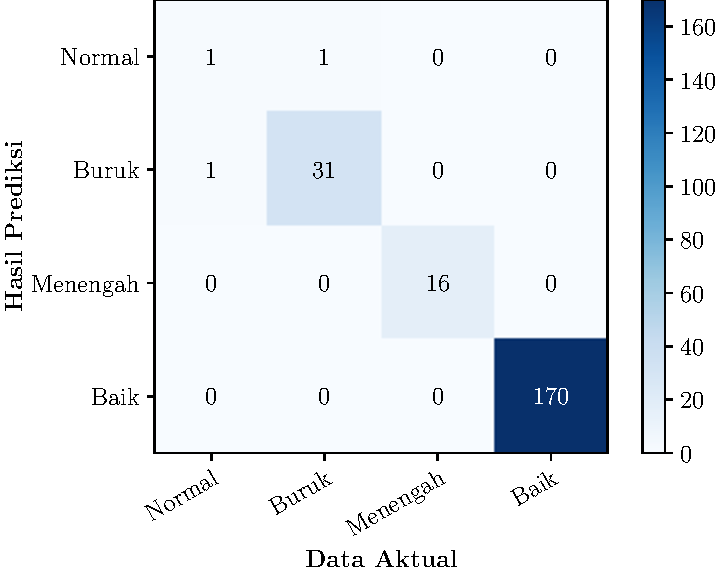
\includegraphics[width=0.6\textwidth]{BAB-4/plot/CM_selu_data_besar.pdf}	
		\captionof{figure}{Studi Kasus 1: \textit{Confusion Matrix} Menggunakan Fungsi Aktivasi \textit{Selu}}
		\label{gambar:CM selu layer DS-1}
	\end{minipage}
}
Kemudian agar lebih mudah dalam memahami informasi yang terdapat pada Gambar \ref{gambar:CM selu layer DS-1}, maka pada gambar tersebut dibuat representasi diagram balok untuk masing-masing nilai presisi dan sensitivitas pada masing-masing kategori. Hal ini dapat dilihat pada penyajian data pada Gambar \ref{gambar:presisi sensitivity selu data besar}. Telah diketahui bahwa akurasi pengujian secara keseluruhan pada sistem ini adalah 99\%, namun jika dilihat secara detail model masih sulit dalam mendiagnosis indeks kesehatan pada kategori "Normal", diperlihatkan pada \textit{confusion matrix} bahwa terdapat satu kategori yang terprediksi sebagai "Buruk". Jika dilakukan penilaian terhadap presisi dan sensitivitas, kategori "normal" merupakan satu-satunya yang memiliki nilai paling buruk. 

\centerline{\begin{minipage}{\linewidth}
		\centering
		\vspace{12 pt}
		%% Creator: Matplotlib, PGF backend
%%
%% To include the figure in your LaTeX document, write
%%   \input{<filename>.pgf}
%%
%% Make sure the required packages are loaded in your preamble
%%   \usepackage{pgf}
%%
%% Figures using additional raster images can only be included by \input if
%% they are in the same directory as the main LaTeX file. For loading figures
%% from other directories you can use the `import` package
%%   \usepackage{import}
%%
%% and then include the figures with
%%   \import{<path to file>}{<filename>.pgf}
%%
%% Matplotlib used the following preamble
%%
\begingroup%
\makeatletter%
\begin{pgfpicture}%
\pgfpathrectangle{\pgfpointorigin}{\pgfqpoint{5.640000in}{3.140000in}}%
\pgfusepath{use as bounding box, clip}%
\begin{pgfscope}%
\pgfsetbuttcap%
\pgfsetmiterjoin%
\pgfsetlinewidth{0.000000pt}%
\definecolor{currentstroke}{rgb}{1.000000,1.000000,1.000000}%
\pgfsetstrokecolor{currentstroke}%
\pgfsetstrokeopacity{0.000000}%
\pgfsetdash{}{0pt}%
\pgfpathmoveto{\pgfqpoint{0.000000in}{0.000000in}}%
\pgfpathlineto{\pgfqpoint{5.640000in}{0.000000in}}%
\pgfpathlineto{\pgfqpoint{5.640000in}{3.140000in}}%
\pgfpathlineto{\pgfqpoint{0.000000in}{3.140000in}}%
\pgfpathclose%
\pgfusepath{}%
\end{pgfscope}%
\begin{pgfscope}%
\pgfsetbuttcap%
\pgfsetmiterjoin%
\definecolor{currentfill}{rgb}{1.000000,1.000000,1.000000}%
\pgfsetfillcolor{currentfill}%
\pgfsetlinewidth{0.000000pt}%
\definecolor{currentstroke}{rgb}{0.000000,0.000000,0.000000}%
\pgfsetstrokecolor{currentstroke}%
\pgfsetstrokeopacity{0.000000}%
\pgfsetdash{}{0pt}%
\pgfpathmoveto{\pgfqpoint{0.453704in}{0.693723in}}%
\pgfpathlineto{\pgfqpoint{2.730000in}{0.693723in}}%
\pgfpathlineto{\pgfqpoint{2.730000in}{3.140000in}}%
\pgfpathlineto{\pgfqpoint{0.453704in}{3.140000in}}%
\pgfpathclose%
\pgfusepath{fill}%
\end{pgfscope}%
\begin{pgfscope}%
\pgfpathrectangle{\pgfqpoint{0.453704in}{0.693723in}}{\pgfqpoint{2.276296in}{2.446277in}}%
\pgfusepath{clip}%
\pgfsetbuttcap%
\pgfsetmiterjoin%
\definecolor{currentfill}{rgb}{0.121569,0.466667,0.705882}%
\pgfsetfillcolor{currentfill}%
\pgfsetlinewidth{0.000000pt}%
\definecolor{currentstroke}{rgb}{0.000000,0.000000,0.000000}%
\pgfsetstrokecolor{currentstroke}%
\pgfsetstrokeopacity{0.000000}%
\pgfsetdash{}{0pt}%
\pgfpathmoveto{\pgfqpoint{0.557172in}{0.693723in}}%
\pgfpathlineto{\pgfqpoint{0.800626in}{0.693723in}}%
\pgfpathlineto{\pgfqpoint{0.800626in}{1.805667in}}%
\pgfpathlineto{\pgfqpoint{0.557172in}{1.805667in}}%
\pgfpathclose%
\pgfusepath{fill}%
\end{pgfscope}%
\begin{pgfscope}%
\pgfpathrectangle{\pgfqpoint{0.453704in}{0.693723in}}{\pgfqpoint{2.276296in}{2.446277in}}%
\pgfusepath{clip}%
\pgfsetbuttcap%
\pgfsetmiterjoin%
\definecolor{currentfill}{rgb}{0.121569,0.466667,0.705882}%
\pgfsetfillcolor{currentfill}%
\pgfsetlinewidth{0.000000pt}%
\definecolor{currentstroke}{rgb}{0.000000,0.000000,0.000000}%
\pgfsetstrokecolor{currentstroke}%
\pgfsetstrokeopacity{0.000000}%
\pgfsetdash{}{0pt}%
\pgfpathmoveto{\pgfqpoint{1.165807in}{0.693723in}}%
\pgfpathlineto{\pgfqpoint{1.409262in}{0.693723in}}%
\pgfpathlineto{\pgfqpoint{1.409262in}{2.848671in}}%
\pgfpathlineto{\pgfqpoint{1.165807in}{2.848671in}}%
\pgfpathclose%
\pgfusepath{fill}%
\end{pgfscope}%
\begin{pgfscope}%
\pgfpathrectangle{\pgfqpoint{0.453704in}{0.693723in}}{\pgfqpoint{2.276296in}{2.446277in}}%
\pgfusepath{clip}%
\pgfsetbuttcap%
\pgfsetmiterjoin%
\definecolor{currentfill}{rgb}{0.121569,0.466667,0.705882}%
\pgfsetfillcolor{currentfill}%
\pgfsetlinewidth{0.000000pt}%
\definecolor{currentstroke}{rgb}{0.000000,0.000000,0.000000}%
\pgfsetstrokecolor{currentstroke}%
\pgfsetstrokeopacity{0.000000}%
\pgfsetdash{}{0pt}%
\pgfpathmoveto{\pgfqpoint{1.774443in}{0.693723in}}%
\pgfpathlineto{\pgfqpoint{2.017897in}{0.693723in}}%
\pgfpathlineto{\pgfqpoint{2.017897in}{2.917611in}}%
\pgfpathlineto{\pgfqpoint{1.774443in}{2.917611in}}%
\pgfpathclose%
\pgfusepath{fill}%
\end{pgfscope}%
\begin{pgfscope}%
\pgfpathrectangle{\pgfqpoint{0.453704in}{0.693723in}}{\pgfqpoint{2.276296in}{2.446277in}}%
\pgfusepath{clip}%
\pgfsetbuttcap%
\pgfsetmiterjoin%
\definecolor{currentfill}{rgb}{0.121569,0.466667,0.705882}%
\pgfsetfillcolor{currentfill}%
\pgfsetlinewidth{0.000000pt}%
\definecolor{currentstroke}{rgb}{0.000000,0.000000,0.000000}%
\pgfsetstrokecolor{currentstroke}%
\pgfsetstrokeopacity{0.000000}%
\pgfsetdash{}{0pt}%
\pgfpathmoveto{\pgfqpoint{2.383078in}{0.693723in}}%
\pgfpathlineto{\pgfqpoint{2.626532in}{0.693723in}}%
\pgfpathlineto{\pgfqpoint{2.626532in}{2.917611in}}%
\pgfpathlineto{\pgfqpoint{2.383078in}{2.917611in}}%
\pgfpathclose%
\pgfusepath{fill}%
\end{pgfscope}%
\begin{pgfscope}%
\pgfsetbuttcap%
\pgfsetroundjoin%
\definecolor{currentfill}{rgb}{0.000000,0.000000,0.000000}%
\pgfsetfillcolor{currentfill}%
\pgfsetlinewidth{0.803000pt}%
\definecolor{currentstroke}{rgb}{0.000000,0.000000,0.000000}%
\pgfsetstrokecolor{currentstroke}%
\pgfsetdash{}{0pt}%
\pgfsys@defobject{currentmarker}{\pgfqpoint{0.000000in}{-0.048611in}}{\pgfqpoint{0.000000in}{0.000000in}}{%
\pgfpathmoveto{\pgfqpoint{0.000000in}{0.000000in}}%
\pgfpathlineto{\pgfqpoint{0.000000in}{-0.048611in}}%
\pgfusepath{stroke,fill}%
}%
\begin{pgfscope}%
\pgfsys@transformshift{0.678899in}{0.693723in}%
\pgfsys@useobject{currentmarker}{}%
\end{pgfscope}%
\end{pgfscope}%
\begin{pgfscope}%
\definecolor{textcolor}{rgb}{0.000000,0.000000,0.000000}%
\pgfsetstrokecolor{textcolor}%
\pgfsetfillcolor{textcolor}%
\pgftext[x=0.678899in,y=0.596500in,right,top,rotate=30.000000]{\color{textcolor}\rmfamily\fontsize{10.000000}{12.000000}\selectfont Normal}%
\end{pgfscope}%
\begin{pgfscope}%
\pgfsetbuttcap%
\pgfsetroundjoin%
\definecolor{currentfill}{rgb}{0.000000,0.000000,0.000000}%
\pgfsetfillcolor{currentfill}%
\pgfsetlinewidth{0.803000pt}%
\definecolor{currentstroke}{rgb}{0.000000,0.000000,0.000000}%
\pgfsetstrokecolor{currentstroke}%
\pgfsetdash{}{0pt}%
\pgfsys@defobject{currentmarker}{\pgfqpoint{0.000000in}{-0.048611in}}{\pgfqpoint{0.000000in}{0.000000in}}{%
\pgfpathmoveto{\pgfqpoint{0.000000in}{0.000000in}}%
\pgfpathlineto{\pgfqpoint{0.000000in}{-0.048611in}}%
\pgfusepath{stroke,fill}%
}%
\begin{pgfscope}%
\pgfsys@transformshift{1.287534in}{0.693723in}%
\pgfsys@useobject{currentmarker}{}%
\end{pgfscope}%
\end{pgfscope}%
\begin{pgfscope}%
\definecolor{textcolor}{rgb}{0.000000,0.000000,0.000000}%
\pgfsetstrokecolor{textcolor}%
\pgfsetfillcolor{textcolor}%
\pgftext[x=1.287534in,y=0.596500in,right,top,rotate=30.000000]{\color{textcolor}\rmfamily\fontsize{10.000000}{12.000000}\selectfont Buruk}%
\end{pgfscope}%
\begin{pgfscope}%
\pgfsetbuttcap%
\pgfsetroundjoin%
\definecolor{currentfill}{rgb}{0.000000,0.000000,0.000000}%
\pgfsetfillcolor{currentfill}%
\pgfsetlinewidth{0.803000pt}%
\definecolor{currentstroke}{rgb}{0.000000,0.000000,0.000000}%
\pgfsetstrokecolor{currentstroke}%
\pgfsetdash{}{0pt}%
\pgfsys@defobject{currentmarker}{\pgfqpoint{0.000000in}{-0.048611in}}{\pgfqpoint{0.000000in}{0.000000in}}{%
\pgfpathmoveto{\pgfqpoint{0.000000in}{0.000000in}}%
\pgfpathlineto{\pgfqpoint{0.000000in}{-0.048611in}}%
\pgfusepath{stroke,fill}%
}%
\begin{pgfscope}%
\pgfsys@transformshift{1.896170in}{0.693723in}%
\pgfsys@useobject{currentmarker}{}%
\end{pgfscope}%
\end{pgfscope}%
\begin{pgfscope}%
\definecolor{textcolor}{rgb}{0.000000,0.000000,0.000000}%
\pgfsetstrokecolor{textcolor}%
\pgfsetfillcolor{textcolor}%
\pgftext[x=1.896170in,y=0.596500in,right,top,rotate=30.000000]{\color{textcolor}\rmfamily\fontsize{10.000000}{12.000000}\selectfont Menengah}%
\end{pgfscope}%
\begin{pgfscope}%
\pgfsetbuttcap%
\pgfsetroundjoin%
\definecolor{currentfill}{rgb}{0.000000,0.000000,0.000000}%
\pgfsetfillcolor{currentfill}%
\pgfsetlinewidth{0.803000pt}%
\definecolor{currentstroke}{rgb}{0.000000,0.000000,0.000000}%
\pgfsetstrokecolor{currentstroke}%
\pgfsetdash{}{0pt}%
\pgfsys@defobject{currentmarker}{\pgfqpoint{0.000000in}{-0.048611in}}{\pgfqpoint{0.000000in}{0.000000in}}{%
\pgfpathmoveto{\pgfqpoint{0.000000in}{0.000000in}}%
\pgfpathlineto{\pgfqpoint{0.000000in}{-0.048611in}}%
\pgfusepath{stroke,fill}%
}%
\begin{pgfscope}%
\pgfsys@transformshift{2.504805in}{0.693723in}%
\pgfsys@useobject{currentmarker}{}%
\end{pgfscope}%
\end{pgfscope}%
\begin{pgfscope}%
\definecolor{textcolor}{rgb}{0.000000,0.000000,0.000000}%
\pgfsetstrokecolor{textcolor}%
\pgfsetfillcolor{textcolor}%
\pgftext[x=2.504805in,y=0.596500in,right,top,rotate=30.000000]{\color{textcolor}\rmfamily\fontsize{10.000000}{12.000000}\selectfont Baik}%
\end{pgfscope}%
\begin{pgfscope}%
\definecolor{textcolor}{rgb}{0.000000,0.000000,0.000000}%
\pgfsetstrokecolor{textcolor}%
\pgfsetfillcolor{textcolor}%
\pgftext[x=1.591852in,y=0.123457in,,top]{\color{textcolor}\rmfamily\fontsize{10.000000}{12.000000}\selectfont Kategori}%
\end{pgfscope}%
\begin{pgfscope}%
\pgfsetbuttcap%
\pgfsetroundjoin%
\definecolor{currentfill}{rgb}{0.000000,0.000000,0.000000}%
\pgfsetfillcolor{currentfill}%
\pgfsetlinewidth{0.803000pt}%
\definecolor{currentstroke}{rgb}{0.000000,0.000000,0.000000}%
\pgfsetstrokecolor{currentstroke}%
\pgfsetdash{}{0pt}%
\pgfsys@defobject{currentmarker}{\pgfqpoint{-0.048611in}{0.000000in}}{\pgfqpoint{-0.000000in}{0.000000in}}{%
\pgfpathmoveto{\pgfqpoint{-0.000000in}{0.000000in}}%
\pgfpathlineto{\pgfqpoint{-0.048611in}{0.000000in}}%
\pgfusepath{stroke,fill}%
}%
\begin{pgfscope}%
\pgfsys@transformshift{0.453704in}{0.693723in}%
\pgfsys@useobject{currentmarker}{}%
\end{pgfscope}%
\end{pgfscope}%
\begin{pgfscope}%
\definecolor{textcolor}{rgb}{0.000000,0.000000,0.000000}%
\pgfsetstrokecolor{textcolor}%
\pgfsetfillcolor{textcolor}%
\pgftext[x=0.179012in, y=0.645497in, left, base]{\color{textcolor}\rmfamily\fontsize{10.000000}{12.000000}\selectfont \(\displaystyle {0.0}\)}%
\end{pgfscope}%
\begin{pgfscope}%
\pgfsetbuttcap%
\pgfsetroundjoin%
\definecolor{currentfill}{rgb}{0.000000,0.000000,0.000000}%
\pgfsetfillcolor{currentfill}%
\pgfsetlinewidth{0.803000pt}%
\definecolor{currentstroke}{rgb}{0.000000,0.000000,0.000000}%
\pgfsetstrokecolor{currentstroke}%
\pgfsetdash{}{0pt}%
\pgfsys@defobject{currentmarker}{\pgfqpoint{-0.048611in}{0.000000in}}{\pgfqpoint{-0.000000in}{0.000000in}}{%
\pgfpathmoveto{\pgfqpoint{-0.000000in}{0.000000in}}%
\pgfpathlineto{\pgfqpoint{-0.048611in}{0.000000in}}%
\pgfusepath{stroke,fill}%
}%
\begin{pgfscope}%
\pgfsys@transformshift{0.453704in}{1.138500in}%
\pgfsys@useobject{currentmarker}{}%
\end{pgfscope}%
\end{pgfscope}%
\begin{pgfscope}%
\definecolor{textcolor}{rgb}{0.000000,0.000000,0.000000}%
\pgfsetstrokecolor{textcolor}%
\pgfsetfillcolor{textcolor}%
\pgftext[x=0.179012in, y=1.090275in, left, base]{\color{textcolor}\rmfamily\fontsize{10.000000}{12.000000}\selectfont \(\displaystyle {0.2}\)}%
\end{pgfscope}%
\begin{pgfscope}%
\pgfsetbuttcap%
\pgfsetroundjoin%
\definecolor{currentfill}{rgb}{0.000000,0.000000,0.000000}%
\pgfsetfillcolor{currentfill}%
\pgfsetlinewidth{0.803000pt}%
\definecolor{currentstroke}{rgb}{0.000000,0.000000,0.000000}%
\pgfsetstrokecolor{currentstroke}%
\pgfsetdash{}{0pt}%
\pgfsys@defobject{currentmarker}{\pgfqpoint{-0.048611in}{0.000000in}}{\pgfqpoint{-0.000000in}{0.000000in}}{%
\pgfpathmoveto{\pgfqpoint{-0.000000in}{0.000000in}}%
\pgfpathlineto{\pgfqpoint{-0.048611in}{0.000000in}}%
\pgfusepath{stroke,fill}%
}%
\begin{pgfscope}%
\pgfsys@transformshift{0.453704in}{1.583278in}%
\pgfsys@useobject{currentmarker}{}%
\end{pgfscope}%
\end{pgfscope}%
\begin{pgfscope}%
\definecolor{textcolor}{rgb}{0.000000,0.000000,0.000000}%
\pgfsetstrokecolor{textcolor}%
\pgfsetfillcolor{textcolor}%
\pgftext[x=0.179012in, y=1.535053in, left, base]{\color{textcolor}\rmfamily\fontsize{10.000000}{12.000000}\selectfont \(\displaystyle {0.4}\)}%
\end{pgfscope}%
\begin{pgfscope}%
\pgfsetbuttcap%
\pgfsetroundjoin%
\definecolor{currentfill}{rgb}{0.000000,0.000000,0.000000}%
\pgfsetfillcolor{currentfill}%
\pgfsetlinewidth{0.803000pt}%
\definecolor{currentstroke}{rgb}{0.000000,0.000000,0.000000}%
\pgfsetstrokecolor{currentstroke}%
\pgfsetdash{}{0pt}%
\pgfsys@defobject{currentmarker}{\pgfqpoint{-0.048611in}{0.000000in}}{\pgfqpoint{-0.000000in}{0.000000in}}{%
\pgfpathmoveto{\pgfqpoint{-0.000000in}{0.000000in}}%
\pgfpathlineto{\pgfqpoint{-0.048611in}{0.000000in}}%
\pgfusepath{stroke,fill}%
}%
\begin{pgfscope}%
\pgfsys@transformshift{0.453704in}{2.028056in}%
\pgfsys@useobject{currentmarker}{}%
\end{pgfscope}%
\end{pgfscope}%
\begin{pgfscope}%
\definecolor{textcolor}{rgb}{0.000000,0.000000,0.000000}%
\pgfsetstrokecolor{textcolor}%
\pgfsetfillcolor{textcolor}%
\pgftext[x=0.179012in, y=1.979831in, left, base]{\color{textcolor}\rmfamily\fontsize{10.000000}{12.000000}\selectfont \(\displaystyle {0.6}\)}%
\end{pgfscope}%
\begin{pgfscope}%
\pgfsetbuttcap%
\pgfsetroundjoin%
\definecolor{currentfill}{rgb}{0.000000,0.000000,0.000000}%
\pgfsetfillcolor{currentfill}%
\pgfsetlinewidth{0.803000pt}%
\definecolor{currentstroke}{rgb}{0.000000,0.000000,0.000000}%
\pgfsetstrokecolor{currentstroke}%
\pgfsetdash{}{0pt}%
\pgfsys@defobject{currentmarker}{\pgfqpoint{-0.048611in}{0.000000in}}{\pgfqpoint{-0.000000in}{0.000000in}}{%
\pgfpathmoveto{\pgfqpoint{-0.000000in}{0.000000in}}%
\pgfpathlineto{\pgfqpoint{-0.048611in}{0.000000in}}%
\pgfusepath{stroke,fill}%
}%
\begin{pgfscope}%
\pgfsys@transformshift{0.453704in}{2.472833in}%
\pgfsys@useobject{currentmarker}{}%
\end{pgfscope}%
\end{pgfscope}%
\begin{pgfscope}%
\definecolor{textcolor}{rgb}{0.000000,0.000000,0.000000}%
\pgfsetstrokecolor{textcolor}%
\pgfsetfillcolor{textcolor}%
\pgftext[x=0.179012in, y=2.424608in, left, base]{\color{textcolor}\rmfamily\fontsize{10.000000}{12.000000}\selectfont \(\displaystyle {0.8}\)}%
\end{pgfscope}%
\begin{pgfscope}%
\pgfsetbuttcap%
\pgfsetroundjoin%
\definecolor{currentfill}{rgb}{0.000000,0.000000,0.000000}%
\pgfsetfillcolor{currentfill}%
\pgfsetlinewidth{0.803000pt}%
\definecolor{currentstroke}{rgb}{0.000000,0.000000,0.000000}%
\pgfsetstrokecolor{currentstroke}%
\pgfsetdash{}{0pt}%
\pgfsys@defobject{currentmarker}{\pgfqpoint{-0.048611in}{0.000000in}}{\pgfqpoint{-0.000000in}{0.000000in}}{%
\pgfpathmoveto{\pgfqpoint{-0.000000in}{0.000000in}}%
\pgfpathlineto{\pgfqpoint{-0.048611in}{0.000000in}}%
\pgfusepath{stroke,fill}%
}%
\begin{pgfscope}%
\pgfsys@transformshift{0.453704in}{2.917611in}%
\pgfsys@useobject{currentmarker}{}%
\end{pgfscope}%
\end{pgfscope}%
\begin{pgfscope}%
\definecolor{textcolor}{rgb}{0.000000,0.000000,0.000000}%
\pgfsetstrokecolor{textcolor}%
\pgfsetfillcolor{textcolor}%
\pgftext[x=0.179012in, y=2.869386in, left, base]{\color{textcolor}\rmfamily\fontsize{10.000000}{12.000000}\selectfont \(\displaystyle {1.0}\)}%
\end{pgfscope}%
\begin{pgfscope}%
\definecolor{textcolor}{rgb}{0.000000,0.000000,0.000000}%
\pgfsetstrokecolor{textcolor}%
\pgfsetfillcolor{textcolor}%
\pgftext[x=0.123457in,y=1.916861in,,bottom,rotate=90.000000]{\color{textcolor}\rmfamily\fontsize{10.000000}{12.000000}\selectfont Presisi}%
\end{pgfscope}%
\begin{pgfscope}%
\pgfsetrectcap%
\pgfsetmiterjoin%
\pgfsetlinewidth{0.803000pt}%
\definecolor{currentstroke}{rgb}{0.000000,0.000000,0.000000}%
\pgfsetstrokecolor{currentstroke}%
\pgfsetdash{}{0pt}%
\pgfpathmoveto{\pgfqpoint{0.453704in}{0.693723in}}%
\pgfpathlineto{\pgfqpoint{0.453704in}{3.140000in}}%
\pgfusepath{stroke}%
\end{pgfscope}%
\begin{pgfscope}%
\pgfsetrectcap%
\pgfsetmiterjoin%
\pgfsetlinewidth{0.803000pt}%
\definecolor{currentstroke}{rgb}{0.000000,0.000000,0.000000}%
\pgfsetstrokecolor{currentstroke}%
\pgfsetdash{}{0pt}%
\pgfpathmoveto{\pgfqpoint{2.730000in}{0.693723in}}%
\pgfpathlineto{\pgfqpoint{2.730000in}{3.140000in}}%
\pgfusepath{stroke}%
\end{pgfscope}%
\begin{pgfscope}%
\pgfsetrectcap%
\pgfsetmiterjoin%
\pgfsetlinewidth{0.803000pt}%
\definecolor{currentstroke}{rgb}{0.000000,0.000000,0.000000}%
\pgfsetstrokecolor{currentstroke}%
\pgfsetdash{}{0pt}%
\pgfpathmoveto{\pgfqpoint{0.453704in}{0.693723in}}%
\pgfpathlineto{\pgfqpoint{2.730000in}{0.693723in}}%
\pgfusepath{stroke}%
\end{pgfscope}%
\begin{pgfscope}%
\pgfsetrectcap%
\pgfsetmiterjoin%
\pgfsetlinewidth{0.803000pt}%
\definecolor{currentstroke}{rgb}{0.000000,0.000000,0.000000}%
\pgfsetstrokecolor{currentstroke}%
\pgfsetdash{}{0pt}%
\pgfpathmoveto{\pgfqpoint{0.453704in}{3.140000in}}%
\pgfpathlineto{\pgfqpoint{2.730000in}{3.140000in}}%
\pgfusepath{stroke}%
\end{pgfscope}%
\begin{pgfscope}%
\definecolor{textcolor}{rgb}{0.000000,0.000000,0.000000}%
\pgfsetstrokecolor{textcolor}%
\pgfsetfillcolor{textcolor}%
\pgftext[x=0.678899in,y=1.827906in,,bottom]{\color{textcolor}\rmfamily\fontsize{9.000000}{10.800000}\selectfont 0.5}%
\end{pgfscope}%
\begin{pgfscope}%
\definecolor{textcolor}{rgb}{0.000000,0.000000,0.000000}%
\pgfsetstrokecolor{textcolor}%
\pgfsetfillcolor{textcolor}%
\pgftext[x=1.287534in,y=2.870909in,,bottom]{\color{textcolor}\rmfamily\fontsize{9.000000}{10.800000}\selectfont 0.969}%
\end{pgfscope}%
\begin{pgfscope}%
\definecolor{textcolor}{rgb}{0.000000,0.000000,0.000000}%
\pgfsetstrokecolor{textcolor}%
\pgfsetfillcolor{textcolor}%
\pgftext[x=1.896170in,y=2.939850in,,bottom]{\color{textcolor}\rmfamily\fontsize{9.000000}{10.800000}\selectfont 1.0}%
\end{pgfscope}%
\begin{pgfscope}%
\definecolor{textcolor}{rgb}{0.000000,0.000000,0.000000}%
\pgfsetstrokecolor{textcolor}%
\pgfsetfillcolor{textcolor}%
\pgftext[x=2.504805in,y=2.939850in,,bottom]{\color{textcolor}\rmfamily\fontsize{9.000000}{10.800000}\selectfont 1.0}%
\end{pgfscope}%
\begin{pgfscope}%
\pgfsetbuttcap%
\pgfsetmiterjoin%
\definecolor{currentfill}{rgb}{1.000000,1.000000,1.000000}%
\pgfsetfillcolor{currentfill}%
\pgfsetlinewidth{0.000000pt}%
\definecolor{currentstroke}{rgb}{0.000000,0.000000,0.000000}%
\pgfsetstrokecolor{currentstroke}%
\pgfsetstrokeopacity{0.000000}%
\pgfsetdash{}{0pt}%
\pgfpathmoveto{\pgfqpoint{3.363704in}{0.693723in}}%
\pgfpathlineto{\pgfqpoint{5.640000in}{0.693723in}}%
\pgfpathlineto{\pgfqpoint{5.640000in}{3.140000in}}%
\pgfpathlineto{\pgfqpoint{3.363704in}{3.140000in}}%
\pgfpathclose%
\pgfusepath{fill}%
\end{pgfscope}%
\begin{pgfscope}%
\pgfpathrectangle{\pgfqpoint{3.363704in}{0.693723in}}{\pgfqpoint{2.276296in}{2.446277in}}%
\pgfusepath{clip}%
\pgfsetbuttcap%
\pgfsetmiterjoin%
\definecolor{currentfill}{rgb}{1.000000,0.498039,0.054902}%
\pgfsetfillcolor{currentfill}%
\pgfsetlinewidth{0.000000pt}%
\definecolor{currentstroke}{rgb}{0.000000,0.000000,0.000000}%
\pgfsetstrokecolor{currentstroke}%
\pgfsetstrokeopacity{0.000000}%
\pgfsetdash{}{0pt}%
\pgfpathmoveto{\pgfqpoint{3.467172in}{0.693723in}}%
\pgfpathlineto{\pgfqpoint{3.710626in}{0.693723in}}%
\pgfpathlineto{\pgfqpoint{3.710626in}{1.805667in}}%
\pgfpathlineto{\pgfqpoint{3.467172in}{1.805667in}}%
\pgfpathclose%
\pgfusepath{fill}%
\end{pgfscope}%
\begin{pgfscope}%
\pgfpathrectangle{\pgfqpoint{3.363704in}{0.693723in}}{\pgfqpoint{2.276296in}{2.446277in}}%
\pgfusepath{clip}%
\pgfsetbuttcap%
\pgfsetmiterjoin%
\definecolor{currentfill}{rgb}{1.000000,0.498039,0.054902}%
\pgfsetfillcolor{currentfill}%
\pgfsetlinewidth{0.000000pt}%
\definecolor{currentstroke}{rgb}{0.000000,0.000000,0.000000}%
\pgfsetstrokecolor{currentstroke}%
\pgfsetstrokeopacity{0.000000}%
\pgfsetdash{}{0pt}%
\pgfpathmoveto{\pgfqpoint{4.075807in}{0.693723in}}%
\pgfpathlineto{\pgfqpoint{4.319262in}{0.693723in}}%
\pgfpathlineto{\pgfqpoint{4.319262in}{2.848671in}}%
\pgfpathlineto{\pgfqpoint{4.075807in}{2.848671in}}%
\pgfpathclose%
\pgfusepath{fill}%
\end{pgfscope}%
\begin{pgfscope}%
\pgfpathrectangle{\pgfqpoint{3.363704in}{0.693723in}}{\pgfqpoint{2.276296in}{2.446277in}}%
\pgfusepath{clip}%
\pgfsetbuttcap%
\pgfsetmiterjoin%
\definecolor{currentfill}{rgb}{1.000000,0.498039,0.054902}%
\pgfsetfillcolor{currentfill}%
\pgfsetlinewidth{0.000000pt}%
\definecolor{currentstroke}{rgb}{0.000000,0.000000,0.000000}%
\pgfsetstrokecolor{currentstroke}%
\pgfsetstrokeopacity{0.000000}%
\pgfsetdash{}{0pt}%
\pgfpathmoveto{\pgfqpoint{4.684443in}{0.693723in}}%
\pgfpathlineto{\pgfqpoint{4.927897in}{0.693723in}}%
\pgfpathlineto{\pgfqpoint{4.927897in}{2.917611in}}%
\pgfpathlineto{\pgfqpoint{4.684443in}{2.917611in}}%
\pgfpathclose%
\pgfusepath{fill}%
\end{pgfscope}%
\begin{pgfscope}%
\pgfpathrectangle{\pgfqpoint{3.363704in}{0.693723in}}{\pgfqpoint{2.276296in}{2.446277in}}%
\pgfusepath{clip}%
\pgfsetbuttcap%
\pgfsetmiterjoin%
\definecolor{currentfill}{rgb}{1.000000,0.498039,0.054902}%
\pgfsetfillcolor{currentfill}%
\pgfsetlinewidth{0.000000pt}%
\definecolor{currentstroke}{rgb}{0.000000,0.000000,0.000000}%
\pgfsetstrokecolor{currentstroke}%
\pgfsetstrokeopacity{0.000000}%
\pgfsetdash{}{0pt}%
\pgfpathmoveto{\pgfqpoint{5.293078in}{0.693723in}}%
\pgfpathlineto{\pgfqpoint{5.536532in}{0.693723in}}%
\pgfpathlineto{\pgfqpoint{5.536532in}{2.917611in}}%
\pgfpathlineto{\pgfqpoint{5.293078in}{2.917611in}}%
\pgfpathclose%
\pgfusepath{fill}%
\end{pgfscope}%
\begin{pgfscope}%
\pgfsetbuttcap%
\pgfsetroundjoin%
\definecolor{currentfill}{rgb}{0.000000,0.000000,0.000000}%
\pgfsetfillcolor{currentfill}%
\pgfsetlinewidth{0.803000pt}%
\definecolor{currentstroke}{rgb}{0.000000,0.000000,0.000000}%
\pgfsetstrokecolor{currentstroke}%
\pgfsetdash{}{0pt}%
\pgfsys@defobject{currentmarker}{\pgfqpoint{0.000000in}{-0.048611in}}{\pgfqpoint{0.000000in}{0.000000in}}{%
\pgfpathmoveto{\pgfqpoint{0.000000in}{0.000000in}}%
\pgfpathlineto{\pgfqpoint{0.000000in}{-0.048611in}}%
\pgfusepath{stroke,fill}%
}%
\begin{pgfscope}%
\pgfsys@transformshift{3.588899in}{0.693723in}%
\pgfsys@useobject{currentmarker}{}%
\end{pgfscope}%
\end{pgfscope}%
\begin{pgfscope}%
\definecolor{textcolor}{rgb}{0.000000,0.000000,0.000000}%
\pgfsetstrokecolor{textcolor}%
\pgfsetfillcolor{textcolor}%
\pgftext[x=3.588899in,y=0.596500in,right,top,rotate=30.000000]{\color{textcolor}\rmfamily\fontsize{10.000000}{12.000000}\selectfont Normal}%
\end{pgfscope}%
\begin{pgfscope}%
\pgfsetbuttcap%
\pgfsetroundjoin%
\definecolor{currentfill}{rgb}{0.000000,0.000000,0.000000}%
\pgfsetfillcolor{currentfill}%
\pgfsetlinewidth{0.803000pt}%
\definecolor{currentstroke}{rgb}{0.000000,0.000000,0.000000}%
\pgfsetstrokecolor{currentstroke}%
\pgfsetdash{}{0pt}%
\pgfsys@defobject{currentmarker}{\pgfqpoint{0.000000in}{-0.048611in}}{\pgfqpoint{0.000000in}{0.000000in}}{%
\pgfpathmoveto{\pgfqpoint{0.000000in}{0.000000in}}%
\pgfpathlineto{\pgfqpoint{0.000000in}{-0.048611in}}%
\pgfusepath{stroke,fill}%
}%
\begin{pgfscope}%
\pgfsys@transformshift{4.197534in}{0.693723in}%
\pgfsys@useobject{currentmarker}{}%
\end{pgfscope}%
\end{pgfscope}%
\begin{pgfscope}%
\definecolor{textcolor}{rgb}{0.000000,0.000000,0.000000}%
\pgfsetstrokecolor{textcolor}%
\pgfsetfillcolor{textcolor}%
\pgftext[x=4.197534in,y=0.596500in,right,top,rotate=30.000000]{\color{textcolor}\rmfamily\fontsize{10.000000}{12.000000}\selectfont Buruk}%
\end{pgfscope}%
\begin{pgfscope}%
\pgfsetbuttcap%
\pgfsetroundjoin%
\definecolor{currentfill}{rgb}{0.000000,0.000000,0.000000}%
\pgfsetfillcolor{currentfill}%
\pgfsetlinewidth{0.803000pt}%
\definecolor{currentstroke}{rgb}{0.000000,0.000000,0.000000}%
\pgfsetstrokecolor{currentstroke}%
\pgfsetdash{}{0pt}%
\pgfsys@defobject{currentmarker}{\pgfqpoint{0.000000in}{-0.048611in}}{\pgfqpoint{0.000000in}{0.000000in}}{%
\pgfpathmoveto{\pgfqpoint{0.000000in}{0.000000in}}%
\pgfpathlineto{\pgfqpoint{0.000000in}{-0.048611in}}%
\pgfusepath{stroke,fill}%
}%
\begin{pgfscope}%
\pgfsys@transformshift{4.806170in}{0.693723in}%
\pgfsys@useobject{currentmarker}{}%
\end{pgfscope}%
\end{pgfscope}%
\begin{pgfscope}%
\definecolor{textcolor}{rgb}{0.000000,0.000000,0.000000}%
\pgfsetstrokecolor{textcolor}%
\pgfsetfillcolor{textcolor}%
\pgftext[x=4.806170in,y=0.596500in,right,top,rotate=30.000000]{\color{textcolor}\rmfamily\fontsize{10.000000}{12.000000}\selectfont Menengah}%
\end{pgfscope}%
\begin{pgfscope}%
\pgfsetbuttcap%
\pgfsetroundjoin%
\definecolor{currentfill}{rgb}{0.000000,0.000000,0.000000}%
\pgfsetfillcolor{currentfill}%
\pgfsetlinewidth{0.803000pt}%
\definecolor{currentstroke}{rgb}{0.000000,0.000000,0.000000}%
\pgfsetstrokecolor{currentstroke}%
\pgfsetdash{}{0pt}%
\pgfsys@defobject{currentmarker}{\pgfqpoint{0.000000in}{-0.048611in}}{\pgfqpoint{0.000000in}{0.000000in}}{%
\pgfpathmoveto{\pgfqpoint{0.000000in}{0.000000in}}%
\pgfpathlineto{\pgfqpoint{0.000000in}{-0.048611in}}%
\pgfusepath{stroke,fill}%
}%
\begin{pgfscope}%
\pgfsys@transformshift{5.414805in}{0.693723in}%
\pgfsys@useobject{currentmarker}{}%
\end{pgfscope}%
\end{pgfscope}%
\begin{pgfscope}%
\definecolor{textcolor}{rgb}{0.000000,0.000000,0.000000}%
\pgfsetstrokecolor{textcolor}%
\pgfsetfillcolor{textcolor}%
\pgftext[x=5.414805in,y=0.596500in,right,top,rotate=30.000000]{\color{textcolor}\rmfamily\fontsize{10.000000}{12.000000}\selectfont Baik}%
\end{pgfscope}%
\begin{pgfscope}%
\definecolor{textcolor}{rgb}{0.000000,0.000000,0.000000}%
\pgfsetstrokecolor{textcolor}%
\pgfsetfillcolor{textcolor}%
\pgftext[x=4.501852in,y=0.123457in,,top]{\color{textcolor}\rmfamily\fontsize{10.000000}{12.000000}\selectfont Kategori}%
\end{pgfscope}%
\begin{pgfscope}%
\pgfsetbuttcap%
\pgfsetroundjoin%
\definecolor{currentfill}{rgb}{0.000000,0.000000,0.000000}%
\pgfsetfillcolor{currentfill}%
\pgfsetlinewidth{0.803000pt}%
\definecolor{currentstroke}{rgb}{0.000000,0.000000,0.000000}%
\pgfsetstrokecolor{currentstroke}%
\pgfsetdash{}{0pt}%
\pgfsys@defobject{currentmarker}{\pgfqpoint{-0.048611in}{0.000000in}}{\pgfqpoint{-0.000000in}{0.000000in}}{%
\pgfpathmoveto{\pgfqpoint{-0.000000in}{0.000000in}}%
\pgfpathlineto{\pgfqpoint{-0.048611in}{0.000000in}}%
\pgfusepath{stroke,fill}%
}%
\begin{pgfscope}%
\pgfsys@transformshift{3.363704in}{0.693723in}%
\pgfsys@useobject{currentmarker}{}%
\end{pgfscope}%
\end{pgfscope}%
\begin{pgfscope}%
\definecolor{textcolor}{rgb}{0.000000,0.000000,0.000000}%
\pgfsetstrokecolor{textcolor}%
\pgfsetfillcolor{textcolor}%
\pgftext[x=3.089012in, y=0.645497in, left, base]{\color{textcolor}\rmfamily\fontsize{10.000000}{12.000000}\selectfont \(\displaystyle {0.0}\)}%
\end{pgfscope}%
\begin{pgfscope}%
\pgfsetbuttcap%
\pgfsetroundjoin%
\definecolor{currentfill}{rgb}{0.000000,0.000000,0.000000}%
\pgfsetfillcolor{currentfill}%
\pgfsetlinewidth{0.803000pt}%
\definecolor{currentstroke}{rgb}{0.000000,0.000000,0.000000}%
\pgfsetstrokecolor{currentstroke}%
\pgfsetdash{}{0pt}%
\pgfsys@defobject{currentmarker}{\pgfqpoint{-0.048611in}{0.000000in}}{\pgfqpoint{-0.000000in}{0.000000in}}{%
\pgfpathmoveto{\pgfqpoint{-0.000000in}{0.000000in}}%
\pgfpathlineto{\pgfqpoint{-0.048611in}{0.000000in}}%
\pgfusepath{stroke,fill}%
}%
\begin{pgfscope}%
\pgfsys@transformshift{3.363704in}{1.138500in}%
\pgfsys@useobject{currentmarker}{}%
\end{pgfscope}%
\end{pgfscope}%
\begin{pgfscope}%
\definecolor{textcolor}{rgb}{0.000000,0.000000,0.000000}%
\pgfsetstrokecolor{textcolor}%
\pgfsetfillcolor{textcolor}%
\pgftext[x=3.089012in, y=1.090275in, left, base]{\color{textcolor}\rmfamily\fontsize{10.000000}{12.000000}\selectfont \(\displaystyle {0.2}\)}%
\end{pgfscope}%
\begin{pgfscope}%
\pgfsetbuttcap%
\pgfsetroundjoin%
\definecolor{currentfill}{rgb}{0.000000,0.000000,0.000000}%
\pgfsetfillcolor{currentfill}%
\pgfsetlinewidth{0.803000pt}%
\definecolor{currentstroke}{rgb}{0.000000,0.000000,0.000000}%
\pgfsetstrokecolor{currentstroke}%
\pgfsetdash{}{0pt}%
\pgfsys@defobject{currentmarker}{\pgfqpoint{-0.048611in}{0.000000in}}{\pgfqpoint{-0.000000in}{0.000000in}}{%
\pgfpathmoveto{\pgfqpoint{-0.000000in}{0.000000in}}%
\pgfpathlineto{\pgfqpoint{-0.048611in}{0.000000in}}%
\pgfusepath{stroke,fill}%
}%
\begin{pgfscope}%
\pgfsys@transformshift{3.363704in}{1.583278in}%
\pgfsys@useobject{currentmarker}{}%
\end{pgfscope}%
\end{pgfscope}%
\begin{pgfscope}%
\definecolor{textcolor}{rgb}{0.000000,0.000000,0.000000}%
\pgfsetstrokecolor{textcolor}%
\pgfsetfillcolor{textcolor}%
\pgftext[x=3.089012in, y=1.535053in, left, base]{\color{textcolor}\rmfamily\fontsize{10.000000}{12.000000}\selectfont \(\displaystyle {0.4}\)}%
\end{pgfscope}%
\begin{pgfscope}%
\pgfsetbuttcap%
\pgfsetroundjoin%
\definecolor{currentfill}{rgb}{0.000000,0.000000,0.000000}%
\pgfsetfillcolor{currentfill}%
\pgfsetlinewidth{0.803000pt}%
\definecolor{currentstroke}{rgb}{0.000000,0.000000,0.000000}%
\pgfsetstrokecolor{currentstroke}%
\pgfsetdash{}{0pt}%
\pgfsys@defobject{currentmarker}{\pgfqpoint{-0.048611in}{0.000000in}}{\pgfqpoint{-0.000000in}{0.000000in}}{%
\pgfpathmoveto{\pgfqpoint{-0.000000in}{0.000000in}}%
\pgfpathlineto{\pgfqpoint{-0.048611in}{0.000000in}}%
\pgfusepath{stroke,fill}%
}%
\begin{pgfscope}%
\pgfsys@transformshift{3.363704in}{2.028056in}%
\pgfsys@useobject{currentmarker}{}%
\end{pgfscope}%
\end{pgfscope}%
\begin{pgfscope}%
\definecolor{textcolor}{rgb}{0.000000,0.000000,0.000000}%
\pgfsetstrokecolor{textcolor}%
\pgfsetfillcolor{textcolor}%
\pgftext[x=3.089012in, y=1.979831in, left, base]{\color{textcolor}\rmfamily\fontsize{10.000000}{12.000000}\selectfont \(\displaystyle {0.6}\)}%
\end{pgfscope}%
\begin{pgfscope}%
\pgfsetbuttcap%
\pgfsetroundjoin%
\definecolor{currentfill}{rgb}{0.000000,0.000000,0.000000}%
\pgfsetfillcolor{currentfill}%
\pgfsetlinewidth{0.803000pt}%
\definecolor{currentstroke}{rgb}{0.000000,0.000000,0.000000}%
\pgfsetstrokecolor{currentstroke}%
\pgfsetdash{}{0pt}%
\pgfsys@defobject{currentmarker}{\pgfqpoint{-0.048611in}{0.000000in}}{\pgfqpoint{-0.000000in}{0.000000in}}{%
\pgfpathmoveto{\pgfqpoint{-0.000000in}{0.000000in}}%
\pgfpathlineto{\pgfqpoint{-0.048611in}{0.000000in}}%
\pgfusepath{stroke,fill}%
}%
\begin{pgfscope}%
\pgfsys@transformshift{3.363704in}{2.472833in}%
\pgfsys@useobject{currentmarker}{}%
\end{pgfscope}%
\end{pgfscope}%
\begin{pgfscope}%
\definecolor{textcolor}{rgb}{0.000000,0.000000,0.000000}%
\pgfsetstrokecolor{textcolor}%
\pgfsetfillcolor{textcolor}%
\pgftext[x=3.089012in, y=2.424608in, left, base]{\color{textcolor}\rmfamily\fontsize{10.000000}{12.000000}\selectfont \(\displaystyle {0.8}\)}%
\end{pgfscope}%
\begin{pgfscope}%
\pgfsetbuttcap%
\pgfsetroundjoin%
\definecolor{currentfill}{rgb}{0.000000,0.000000,0.000000}%
\pgfsetfillcolor{currentfill}%
\pgfsetlinewidth{0.803000pt}%
\definecolor{currentstroke}{rgb}{0.000000,0.000000,0.000000}%
\pgfsetstrokecolor{currentstroke}%
\pgfsetdash{}{0pt}%
\pgfsys@defobject{currentmarker}{\pgfqpoint{-0.048611in}{0.000000in}}{\pgfqpoint{-0.000000in}{0.000000in}}{%
\pgfpathmoveto{\pgfqpoint{-0.000000in}{0.000000in}}%
\pgfpathlineto{\pgfqpoint{-0.048611in}{0.000000in}}%
\pgfusepath{stroke,fill}%
}%
\begin{pgfscope}%
\pgfsys@transformshift{3.363704in}{2.917611in}%
\pgfsys@useobject{currentmarker}{}%
\end{pgfscope}%
\end{pgfscope}%
\begin{pgfscope}%
\definecolor{textcolor}{rgb}{0.000000,0.000000,0.000000}%
\pgfsetstrokecolor{textcolor}%
\pgfsetfillcolor{textcolor}%
\pgftext[x=3.089012in, y=2.869386in, left, base]{\color{textcolor}\rmfamily\fontsize{10.000000}{12.000000}\selectfont \(\displaystyle {1.0}\)}%
\end{pgfscope}%
\begin{pgfscope}%
\definecolor{textcolor}{rgb}{0.000000,0.000000,0.000000}%
\pgfsetstrokecolor{textcolor}%
\pgfsetfillcolor{textcolor}%
\pgftext[x=3.033457in,y=1.916861in,,bottom,rotate=90.000000]{\color{textcolor}\rmfamily\fontsize{10.000000}{12.000000}\selectfont Sensitivitas}%
\end{pgfscope}%
\begin{pgfscope}%
\pgfsetrectcap%
\pgfsetmiterjoin%
\pgfsetlinewidth{0.803000pt}%
\definecolor{currentstroke}{rgb}{0.000000,0.000000,0.000000}%
\pgfsetstrokecolor{currentstroke}%
\pgfsetdash{}{0pt}%
\pgfpathmoveto{\pgfqpoint{3.363704in}{0.693723in}}%
\pgfpathlineto{\pgfqpoint{3.363704in}{3.140000in}}%
\pgfusepath{stroke}%
\end{pgfscope}%
\begin{pgfscope}%
\pgfsetrectcap%
\pgfsetmiterjoin%
\pgfsetlinewidth{0.803000pt}%
\definecolor{currentstroke}{rgb}{0.000000,0.000000,0.000000}%
\pgfsetstrokecolor{currentstroke}%
\pgfsetdash{}{0pt}%
\pgfpathmoveto{\pgfqpoint{5.640000in}{0.693723in}}%
\pgfpathlineto{\pgfqpoint{5.640000in}{3.140000in}}%
\pgfusepath{stroke}%
\end{pgfscope}%
\begin{pgfscope}%
\pgfsetrectcap%
\pgfsetmiterjoin%
\pgfsetlinewidth{0.803000pt}%
\definecolor{currentstroke}{rgb}{0.000000,0.000000,0.000000}%
\pgfsetstrokecolor{currentstroke}%
\pgfsetdash{}{0pt}%
\pgfpathmoveto{\pgfqpoint{3.363704in}{0.693723in}}%
\pgfpathlineto{\pgfqpoint{5.640000in}{0.693723in}}%
\pgfusepath{stroke}%
\end{pgfscope}%
\begin{pgfscope}%
\pgfsetrectcap%
\pgfsetmiterjoin%
\pgfsetlinewidth{0.803000pt}%
\definecolor{currentstroke}{rgb}{0.000000,0.000000,0.000000}%
\pgfsetstrokecolor{currentstroke}%
\pgfsetdash{}{0pt}%
\pgfpathmoveto{\pgfqpoint{3.363704in}{3.140000in}}%
\pgfpathlineto{\pgfqpoint{5.640000in}{3.140000in}}%
\pgfusepath{stroke}%
\end{pgfscope}%
\begin{pgfscope}%
\definecolor{textcolor}{rgb}{0.000000,0.000000,0.000000}%
\pgfsetstrokecolor{textcolor}%
\pgfsetfillcolor{textcolor}%
\pgftext[x=3.588899in,y=1.827906in,,bottom]{\color{textcolor}\rmfamily\fontsize{9.000000}{10.800000}\selectfont 0.5}%
\end{pgfscope}%
\begin{pgfscope}%
\definecolor{textcolor}{rgb}{0.000000,0.000000,0.000000}%
\pgfsetstrokecolor{textcolor}%
\pgfsetfillcolor{textcolor}%
\pgftext[x=4.197534in,y=2.870909in,,bottom]{\color{textcolor}\rmfamily\fontsize{9.000000}{10.800000}\selectfont 0.969}%
\end{pgfscope}%
\begin{pgfscope}%
\definecolor{textcolor}{rgb}{0.000000,0.000000,0.000000}%
\pgfsetstrokecolor{textcolor}%
\pgfsetfillcolor{textcolor}%
\pgftext[x=4.806170in,y=2.939850in,,bottom]{\color{textcolor}\rmfamily\fontsize{9.000000}{10.800000}\selectfont 1.0}%
\end{pgfscope}%
\begin{pgfscope}%
\definecolor{textcolor}{rgb}{0.000000,0.000000,0.000000}%
\pgfsetstrokecolor{textcolor}%
\pgfsetfillcolor{textcolor}%
\pgftext[x=5.414805in,y=2.939850in,,bottom]{\color{textcolor}\rmfamily\fontsize{9.000000}{10.800000}\selectfont 1.0}%
\end{pgfscope}%
\end{pgfpicture}%
\makeatother%
\endgroup%

		\captionof{figure}{Studi Kasus 1: Presisi Percobaan Perubahan Layer}
		\label{gambar:presisi sensitivity selu data besar}
\end{minipage}}

Pada dasarnnya performa model pada saat mendiagnosis kategori "Normal" yang buruk bukan disebabkan oleh model yang digunakan. Namun, jika melihat karakteristik dari set data 1 yang digunakan pada percobaan ini, berdasarkan Gambar \ref{gambar:pie dataset-1} dapat dilihat bahwa data target berupa kategori "Normal" merupakan yang paling sedikit dibandingkan yang lainnya atau jika ditinjau dari sisi kuantitas hanya 1\% dari total keseluruhan data. Pada kondisi tersebut saat proses pelatihan, model lebih sering dihadapkan kategori dengan jumlah yang lebih banyak akibatnya lebih sulit mengenali kategori dengan jumlah sedikit. \par
Secara umum model yang baik adalah yang tidak \textit{overfiting} dimana akurasi pelatihan sangat baik namun pada proses pengujian model memiliki akurasi yang buruk. Hal ini untuk menghindari agar adanya data pencilan tidak ikut terlatih dalam model.
Pada kasus diagnosis indeks kesehatan transformator daya kurangnya nilai presisi dan sensitivitas pada kategori "Normal" dapat disebabkan karena model menganggap kategori tersebut sebagai sebuah data pencilan sehingga lebih banyak diabaikan. Berdasarkan hasil percobaan ini maka dapat diperoleh informasi bahwa penggunaan data yang tidak seimbang sebaiknya dihindari dalam proses percobaan pada \textit{machine learning} jika model yang diinginkan dapat mendiagnosis setiap kelas dengan baik.

\subsection{Perubahan Pembagian Data dengan Rasio 8:2}
Pada percobaan ini dilakukan dengan menggunakan data yang dipecah menjadi data pelatihan dan data pengujian dengan perbandingan 8:2. 80\% data pertama akan digunakan dalam melatih model agar mengenali pola data dan 20\% data sisanya digunakan dalam mengevaluasi model. Tujuan dari percobaan ini adalah menambah jumlah data yang dilatih agar model dapat lebih mengenal pola data. Model yang digunakan adalah model terbaik pada percobaan sebelumnya yakni dengan menggunakan model dengan dua \textit{hidden layer} serta dengan menggunakan fungsi aktivasi \textit{selu}. Hasil dari percobaan tersebut dapat dilihat pada Gambar \ref{gambar:perbandingan rasio data besar} dan Gambar \ref{gambar:scatter rasio data besar} yang merupakan nilai akurasi rata-rata dan persebaran data percobaan.

\centerline{
	\begin{minipage}{\linewidth}
		\vspace{12 pt}
		\centering
		%% Creator: Matplotlib, PGF backend
%%
%% To include the figure in your LaTeX document, write
%%   \input{<filename>.pgf}
%%
%% Make sure the required packages are loaded in your preamble
%%   \usepackage{pgf}
%%
%% Figures using additional raster images can only be included by \input if
%% they are in the same directory as the main LaTeX file. For loading figures
%% from other directories you can use the `import` package
%%   \usepackage{import}
%%
%% and then include the figures with
%%   \import{<path to file>}{<filename>.pgf}
%%
%% Matplotlib used the following preamble
%%
\begingroup%
\makeatletter%
\begin{pgfpicture}%
\pgfpathrectangle{\pgfpointorigin}{\pgfqpoint{3.623149in}{2.485679in}}%
\pgfusepath{use as bounding box, clip}%
\begin{pgfscope}%
\pgfsetbuttcap%
\pgfsetmiterjoin%
\pgfsetlinewidth{0.000000pt}%
\definecolor{currentstroke}{rgb}{1.000000,1.000000,1.000000}%
\pgfsetstrokecolor{currentstroke}%
\pgfsetstrokeopacity{0.000000}%
\pgfsetdash{}{0pt}%
\pgfpathmoveto{\pgfqpoint{0.000000in}{0.000000in}}%
\pgfpathlineto{\pgfqpoint{3.623149in}{0.000000in}}%
\pgfpathlineto{\pgfqpoint{3.623149in}{2.485679in}}%
\pgfpathlineto{\pgfqpoint{0.000000in}{2.485679in}}%
\pgfpathclose%
\pgfusepath{}%
\end{pgfscope}%
\begin{pgfscope}%
\pgfsetbuttcap%
\pgfsetmiterjoin%
\definecolor{currentfill}{rgb}{1.000000,1.000000,1.000000}%
\pgfsetfillcolor{currentfill}%
\pgfsetlinewidth{0.000000pt}%
\definecolor{currentstroke}{rgb}{0.000000,0.000000,0.000000}%
\pgfsetstrokecolor{currentstroke}%
\pgfsetstrokeopacity{0.000000}%
\pgfsetdash{}{0pt}%
\pgfpathmoveto{\pgfqpoint{0.523149in}{0.220679in}}%
\pgfpathlineto{\pgfqpoint{3.623149in}{0.220679in}}%
\pgfpathlineto{\pgfqpoint{3.623149in}{2.485679in}}%
\pgfpathlineto{\pgfqpoint{0.523149in}{2.485679in}}%
\pgfpathclose%
\pgfusepath{fill}%
\end{pgfscope}%
\begin{pgfscope}%
\pgfpathrectangle{\pgfqpoint{0.523149in}{0.220679in}}{\pgfqpoint{3.100000in}{2.265000in}}%
\pgfusepath{clip}%
\pgfsetbuttcap%
\pgfsetmiterjoin%
\definecolor{currentfill}{rgb}{0.121569,0.466667,0.705882}%
\pgfsetfillcolor{currentfill}%
\pgfsetlinewidth{0.000000pt}%
\definecolor{currentstroke}{rgb}{0.000000,0.000000,0.000000}%
\pgfsetstrokecolor{currentstroke}%
\pgfsetstrokeopacity{0.000000}%
\pgfsetdash{}{0pt}%
\pgfpathmoveto{\pgfqpoint{1.220649in}{-8.015685in}}%
\pgfpathlineto{\pgfqpoint{1.685649in}{-8.015685in}}%
\pgfpathlineto{\pgfqpoint{1.685649in}{2.161654in}}%
\pgfpathlineto{\pgfqpoint{1.220649in}{2.161654in}}%
\pgfpathclose%
\pgfusepath{fill}%
\end{pgfscope}%
\begin{pgfscope}%
\pgfpathrectangle{\pgfqpoint{0.523149in}{0.220679in}}{\pgfqpoint{3.100000in}{2.265000in}}%
\pgfusepath{clip}%
\pgfsetbuttcap%
\pgfsetmiterjoin%
\definecolor{currentfill}{rgb}{1.000000,0.498039,0.054902}%
\pgfsetfillcolor{currentfill}%
\pgfsetlinewidth{0.000000pt}%
\definecolor{currentstroke}{rgb}{0.000000,0.000000,0.000000}%
\pgfsetstrokecolor{currentstroke}%
\pgfsetstrokeopacity{0.000000}%
\pgfsetdash{}{0pt}%
\pgfpathmoveto{\pgfqpoint{2.460649in}{-8.015685in}}%
\pgfpathlineto{\pgfqpoint{2.925649in}{-8.015685in}}%
\pgfpathlineto{\pgfqpoint{2.925649in}{1.891927in}}%
\pgfpathlineto{\pgfqpoint{2.460649in}{1.891927in}}%
\pgfpathclose%
\pgfusepath{fill}%
\end{pgfscope}%
\begin{pgfscope}%
\pgfsetbuttcap%
\pgfsetroundjoin%
\definecolor{currentfill}{rgb}{0.000000,0.000000,0.000000}%
\pgfsetfillcolor{currentfill}%
\pgfsetlinewidth{0.803000pt}%
\definecolor{currentstroke}{rgb}{0.000000,0.000000,0.000000}%
\pgfsetstrokecolor{currentstroke}%
\pgfsetdash{}{0pt}%
\pgfsys@defobject{currentmarker}{\pgfqpoint{0.000000in}{-0.048611in}}{\pgfqpoint{0.000000in}{0.000000in}}{%
\pgfpathmoveto{\pgfqpoint{0.000000in}{0.000000in}}%
\pgfpathlineto{\pgfqpoint{0.000000in}{-0.048611in}}%
\pgfusepath{stroke,fill}%
}%
\begin{pgfscope}%
\pgfsys@transformshift{1.453149in}{0.220679in}%
\pgfsys@useobject{currentmarker}{}%
\end{pgfscope}%
\end{pgfscope}%
\begin{pgfscope}%
\definecolor{textcolor}{rgb}{0.000000,0.000000,0.000000}%
\pgfsetstrokecolor{textcolor}%
\pgfsetfillcolor{textcolor}%
\pgftext[x=1.453149in,y=0.123457in,,top]{\color{textcolor}\rmfamily\fontsize{10.000000}{12.000000}\selectfont pelatihan}%
\end{pgfscope}%
\begin{pgfscope}%
\pgfsetbuttcap%
\pgfsetroundjoin%
\definecolor{currentfill}{rgb}{0.000000,0.000000,0.000000}%
\pgfsetfillcolor{currentfill}%
\pgfsetlinewidth{0.803000pt}%
\definecolor{currentstroke}{rgb}{0.000000,0.000000,0.000000}%
\pgfsetstrokecolor{currentstroke}%
\pgfsetdash{}{0pt}%
\pgfsys@defobject{currentmarker}{\pgfqpoint{0.000000in}{-0.048611in}}{\pgfqpoint{0.000000in}{0.000000in}}{%
\pgfpathmoveto{\pgfqpoint{0.000000in}{0.000000in}}%
\pgfpathlineto{\pgfqpoint{0.000000in}{-0.048611in}}%
\pgfusepath{stroke,fill}%
}%
\begin{pgfscope}%
\pgfsys@transformshift{2.693149in}{0.220679in}%
\pgfsys@useobject{currentmarker}{}%
\end{pgfscope}%
\end{pgfscope}%
\begin{pgfscope}%
\definecolor{textcolor}{rgb}{0.000000,0.000000,0.000000}%
\pgfsetstrokecolor{textcolor}%
\pgfsetfillcolor{textcolor}%
\pgftext[x=2.693149in,y=0.123457in,,top]{\color{textcolor}\rmfamily\fontsize{10.000000}{12.000000}\selectfont pengujian}%
\end{pgfscope}%
\begin{pgfscope}%
\pgfsetbuttcap%
\pgfsetroundjoin%
\definecolor{currentfill}{rgb}{0.000000,0.000000,0.000000}%
\pgfsetfillcolor{currentfill}%
\pgfsetlinewidth{0.803000pt}%
\definecolor{currentstroke}{rgb}{0.000000,0.000000,0.000000}%
\pgfsetstrokecolor{currentstroke}%
\pgfsetdash{}{0pt}%
\pgfsys@defobject{currentmarker}{\pgfqpoint{-0.048611in}{0.000000in}}{\pgfqpoint{-0.000000in}{0.000000in}}{%
\pgfpathmoveto{\pgfqpoint{-0.000000in}{0.000000in}}%
\pgfpathlineto{\pgfqpoint{-0.048611in}{0.000000in}}%
\pgfusepath{stroke,fill}%
}%
\begin{pgfscope}%
\pgfsys@transformshift{0.523149in}{0.220679in}%
\pgfsys@useobject{currentmarker}{}%
\end{pgfscope}%
\end{pgfscope}%
\begin{pgfscope}%
\definecolor{textcolor}{rgb}{0.000000,0.000000,0.000000}%
\pgfsetstrokecolor{textcolor}%
\pgfsetfillcolor{textcolor}%
\pgftext[x=0.179012in, y=0.172454in, left, base]{\color{textcolor}\rmfamily\fontsize{10.000000}{12.000000}\selectfont \(\displaystyle {0.80}\)}%
\end{pgfscope}%
\begin{pgfscope}%
\pgfsetbuttcap%
\pgfsetroundjoin%
\definecolor{currentfill}{rgb}{0.000000,0.000000,0.000000}%
\pgfsetfillcolor{currentfill}%
\pgfsetlinewidth{0.803000pt}%
\definecolor{currentstroke}{rgb}{0.000000,0.000000,0.000000}%
\pgfsetstrokecolor{currentstroke}%
\pgfsetdash{}{0pt}%
\pgfsys@defobject{currentmarker}{\pgfqpoint{-0.048611in}{0.000000in}}{\pgfqpoint{-0.000000in}{0.000000in}}{%
\pgfpathmoveto{\pgfqpoint{-0.000000in}{0.000000in}}%
\pgfpathlineto{\pgfqpoint{-0.048611in}{0.000000in}}%
\pgfusepath{stroke,fill}%
}%
\begin{pgfscope}%
\pgfsys@transformshift{0.523149in}{0.735452in}%
\pgfsys@useobject{currentmarker}{}%
\end{pgfscope}%
\end{pgfscope}%
\begin{pgfscope}%
\definecolor{textcolor}{rgb}{0.000000,0.000000,0.000000}%
\pgfsetstrokecolor{textcolor}%
\pgfsetfillcolor{textcolor}%
\pgftext[x=0.179012in, y=0.687226in, left, base]{\color{textcolor}\rmfamily\fontsize{10.000000}{12.000000}\selectfont \(\displaystyle {0.85}\)}%
\end{pgfscope}%
\begin{pgfscope}%
\pgfsetbuttcap%
\pgfsetroundjoin%
\definecolor{currentfill}{rgb}{0.000000,0.000000,0.000000}%
\pgfsetfillcolor{currentfill}%
\pgfsetlinewidth{0.803000pt}%
\definecolor{currentstroke}{rgb}{0.000000,0.000000,0.000000}%
\pgfsetstrokecolor{currentstroke}%
\pgfsetdash{}{0pt}%
\pgfsys@defobject{currentmarker}{\pgfqpoint{-0.048611in}{0.000000in}}{\pgfqpoint{-0.000000in}{0.000000in}}{%
\pgfpathmoveto{\pgfqpoint{-0.000000in}{0.000000in}}%
\pgfpathlineto{\pgfqpoint{-0.048611in}{0.000000in}}%
\pgfusepath{stroke,fill}%
}%
\begin{pgfscope}%
\pgfsys@transformshift{0.523149in}{1.250224in}%
\pgfsys@useobject{currentmarker}{}%
\end{pgfscope}%
\end{pgfscope}%
\begin{pgfscope}%
\definecolor{textcolor}{rgb}{0.000000,0.000000,0.000000}%
\pgfsetstrokecolor{textcolor}%
\pgfsetfillcolor{textcolor}%
\pgftext[x=0.179012in, y=1.201999in, left, base]{\color{textcolor}\rmfamily\fontsize{10.000000}{12.000000}\selectfont \(\displaystyle {0.90}\)}%
\end{pgfscope}%
\begin{pgfscope}%
\pgfsetbuttcap%
\pgfsetroundjoin%
\definecolor{currentfill}{rgb}{0.000000,0.000000,0.000000}%
\pgfsetfillcolor{currentfill}%
\pgfsetlinewidth{0.803000pt}%
\definecolor{currentstroke}{rgb}{0.000000,0.000000,0.000000}%
\pgfsetstrokecolor{currentstroke}%
\pgfsetdash{}{0pt}%
\pgfsys@defobject{currentmarker}{\pgfqpoint{-0.048611in}{0.000000in}}{\pgfqpoint{-0.000000in}{0.000000in}}{%
\pgfpathmoveto{\pgfqpoint{-0.000000in}{0.000000in}}%
\pgfpathlineto{\pgfqpoint{-0.048611in}{0.000000in}}%
\pgfusepath{stroke,fill}%
}%
\begin{pgfscope}%
\pgfsys@transformshift{0.523149in}{1.764997in}%
\pgfsys@useobject{currentmarker}{}%
\end{pgfscope}%
\end{pgfscope}%
\begin{pgfscope}%
\definecolor{textcolor}{rgb}{0.000000,0.000000,0.000000}%
\pgfsetstrokecolor{textcolor}%
\pgfsetfillcolor{textcolor}%
\pgftext[x=0.179012in, y=1.716772in, left, base]{\color{textcolor}\rmfamily\fontsize{10.000000}{12.000000}\selectfont \(\displaystyle {0.95}\)}%
\end{pgfscope}%
\begin{pgfscope}%
\pgfsetbuttcap%
\pgfsetroundjoin%
\definecolor{currentfill}{rgb}{0.000000,0.000000,0.000000}%
\pgfsetfillcolor{currentfill}%
\pgfsetlinewidth{0.803000pt}%
\definecolor{currentstroke}{rgb}{0.000000,0.000000,0.000000}%
\pgfsetstrokecolor{currentstroke}%
\pgfsetdash{}{0pt}%
\pgfsys@defobject{currentmarker}{\pgfqpoint{-0.048611in}{0.000000in}}{\pgfqpoint{-0.000000in}{0.000000in}}{%
\pgfpathmoveto{\pgfqpoint{-0.000000in}{0.000000in}}%
\pgfpathlineto{\pgfqpoint{-0.048611in}{0.000000in}}%
\pgfusepath{stroke,fill}%
}%
\begin{pgfscope}%
\pgfsys@transformshift{0.523149in}{2.279770in}%
\pgfsys@useobject{currentmarker}{}%
\end{pgfscope}%
\end{pgfscope}%
\begin{pgfscope}%
\definecolor{textcolor}{rgb}{0.000000,0.000000,0.000000}%
\pgfsetstrokecolor{textcolor}%
\pgfsetfillcolor{textcolor}%
\pgftext[x=0.179012in, y=2.231545in, left, base]{\color{textcolor}\rmfamily\fontsize{10.000000}{12.000000}\selectfont \(\displaystyle {1.00}\)}%
\end{pgfscope}%
\begin{pgfscope}%
\definecolor{textcolor}{rgb}{0.000000,0.000000,0.000000}%
\pgfsetstrokecolor{textcolor}%
\pgfsetfillcolor{textcolor}%
\pgftext[x=0.123457in,y=1.353179in,,bottom,rotate=90.000000]{\color{textcolor}\rmfamily\fontsize{10.000000}{12.000000}\selectfont Akurasi}%
\end{pgfscope}%
\begin{pgfscope}%
\pgfpathrectangle{\pgfqpoint{0.523149in}{0.220679in}}{\pgfqpoint{3.100000in}{2.265000in}}%
\pgfusepath{clip}%
\pgfsetbuttcap%
\pgfsetroundjoin%
\pgfsetlinewidth{1.505625pt}%
\definecolor{currentstroke}{rgb}{0.000000,0.000000,0.000000}%
\pgfsetstrokecolor{currentstroke}%
\pgfsetdash{}{0pt}%
\pgfpathmoveto{\pgfqpoint{1.453149in}{1.941166in}}%
\pgfpathlineto{\pgfqpoint{1.453149in}{2.382142in}}%
\pgfusepath{stroke}%
\end{pgfscope}%
\begin{pgfscope}%
\pgfpathrectangle{\pgfqpoint{0.523149in}{0.220679in}}{\pgfqpoint{3.100000in}{2.265000in}}%
\pgfusepath{clip}%
\pgfsetbuttcap%
\pgfsetroundjoin%
\pgfsetlinewidth{1.505625pt}%
\definecolor{currentstroke}{rgb}{0.000000,0.000000,0.000000}%
\pgfsetstrokecolor{currentstroke}%
\pgfsetdash{}{0pt}%
\pgfpathmoveto{\pgfqpoint{2.693149in}{1.581085in}}%
\pgfpathlineto{\pgfqpoint{2.693149in}{2.202770in}}%
\pgfusepath{stroke}%
\end{pgfscope}%
\begin{pgfscope}%
\pgfsetrectcap%
\pgfsetmiterjoin%
\pgfsetlinewidth{0.803000pt}%
\definecolor{currentstroke}{rgb}{0.000000,0.000000,0.000000}%
\pgfsetstrokecolor{currentstroke}%
\pgfsetdash{}{0pt}%
\pgfpathmoveto{\pgfqpoint{0.523149in}{0.220679in}}%
\pgfpathlineto{\pgfqpoint{0.523149in}{2.485679in}}%
\pgfusepath{stroke}%
\end{pgfscope}%
\begin{pgfscope}%
\pgfsetrectcap%
\pgfsetmiterjoin%
\pgfsetlinewidth{0.803000pt}%
\definecolor{currentstroke}{rgb}{0.000000,0.000000,0.000000}%
\pgfsetstrokecolor{currentstroke}%
\pgfsetdash{}{0pt}%
\pgfpathmoveto{\pgfqpoint{3.623149in}{0.220679in}}%
\pgfpathlineto{\pgfqpoint{3.623149in}{2.485679in}}%
\pgfusepath{stroke}%
\end{pgfscope}%
\begin{pgfscope}%
\pgfsetrectcap%
\pgfsetmiterjoin%
\pgfsetlinewidth{0.803000pt}%
\definecolor{currentstroke}{rgb}{0.000000,0.000000,0.000000}%
\pgfsetstrokecolor{currentstroke}%
\pgfsetdash{}{0pt}%
\pgfpathmoveto{\pgfqpoint{0.523149in}{0.220679in}}%
\pgfpathlineto{\pgfqpoint{3.623149in}{0.220679in}}%
\pgfusepath{stroke}%
\end{pgfscope}%
\begin{pgfscope}%
\pgfsetrectcap%
\pgfsetmiterjoin%
\pgfsetlinewidth{0.803000pt}%
\definecolor{currentstroke}{rgb}{0.000000,0.000000,0.000000}%
\pgfsetstrokecolor{currentstroke}%
\pgfsetdash{}{0pt}%
\pgfpathmoveto{\pgfqpoint{0.523149in}{2.485679in}}%
\pgfpathlineto{\pgfqpoint{3.623149in}{2.485679in}}%
\pgfusepath{stroke}%
\end{pgfscope}%
\begin{pgfscope}%
\definecolor{textcolor}{rgb}{0.000000,0.000000,0.000000}%
\pgfsetstrokecolor{textcolor}%
\pgfsetfillcolor{textcolor}%
\pgftext[x=1.515149in,y=2.207702in,left,bottom]{\color{textcolor}\rmfamily\fontsize{9.000000}{10.800000}\selectfont 0.989}%
\end{pgfscope}%
\begin{pgfscope}%
\definecolor{textcolor}{rgb}{0.000000,0.000000,0.000000}%
\pgfsetstrokecolor{textcolor}%
\pgfsetfillcolor{textcolor}%
\pgftext[x=2.755149in,y=1.929724in,left,bottom]{\color{textcolor}\rmfamily\fontsize{9.000000}{10.800000}\selectfont 0.989}%
\end{pgfscope}%
\end{pgfpicture}%
\makeatother%
\endgroup%

		\captionof{figure}{Studi Kasus 1: Akurasi Percobaan Menggunakan Rasio Data Pelatihan dan Pengujian 8:2}
		\label{gambar:perbandingan rasio data besar}
	\end{minipage}
}

\centerline{\begin{minipage}{\linewidth}
		\centering
		\vspace{12 pt}
		%% Creator: Matplotlib, PGF backend
%%
%% To include the figure in your LaTeX document, write
%%   \input{<filename>.pgf}
%%
%% Make sure the required packages are loaded in your preamble
%%   \usepackage{pgf}
%%
%% Figures using additional raster images can only be included by \input if
%% they are in the same directory as the main LaTeX file. For loading figures
%% from other directories you can use the `import` package
%%   \usepackage{import}
%%
%% and then include the figures with
%%   \import{<path to file>}{<filename>.pgf}
%%
%% Matplotlib used the following preamble
%%
\begingroup%
\makeatletter%
\begin{pgfpicture}%
\pgfpathrectangle{\pgfpointorigin}{\pgfqpoint{5.995649in}{2.999722in}}%
\pgfusepath{use as bounding box, clip}%
\begin{pgfscope}%
\pgfsetbuttcap%
\pgfsetmiterjoin%
\pgfsetlinewidth{0.000000pt}%
\definecolor{currentstroke}{rgb}{1.000000,1.000000,1.000000}%
\pgfsetstrokecolor{currentstroke}%
\pgfsetstrokeopacity{0.000000}%
\pgfsetdash{}{0pt}%
\pgfpathmoveto{\pgfqpoint{0.000000in}{0.000000in}}%
\pgfpathlineto{\pgfqpoint{5.995649in}{0.000000in}}%
\pgfpathlineto{\pgfqpoint{5.995649in}{2.999722in}}%
\pgfpathlineto{\pgfqpoint{0.000000in}{2.999722in}}%
\pgfpathclose%
\pgfusepath{}%
\end{pgfscope}%
\begin{pgfscope}%
\pgfsetbuttcap%
\pgfsetmiterjoin%
\definecolor{currentfill}{rgb}{1.000000,1.000000,1.000000}%
\pgfsetfillcolor{currentfill}%
\pgfsetlinewidth{0.000000pt}%
\definecolor{currentstroke}{rgb}{0.000000,0.000000,0.000000}%
\pgfsetstrokecolor{currentstroke}%
\pgfsetstrokeopacity{0.000000}%
\pgfsetdash{}{0pt}%
\pgfpathmoveto{\pgfqpoint{0.523149in}{0.399691in}}%
\pgfpathlineto{\pgfqpoint{2.925510in}{0.399691in}}%
\pgfpathlineto{\pgfqpoint{2.925510in}{2.951497in}}%
\pgfpathlineto{\pgfqpoint{0.523149in}{2.951497in}}%
\pgfpathclose%
\pgfusepath{fill}%
\end{pgfscope}%
\begin{pgfscope}%
\pgfpathrectangle{\pgfqpoint{0.523149in}{0.399691in}}{\pgfqpoint{2.402362in}{2.551806in}}%
\pgfusepath{clip}%
\pgfsetbuttcap%
\pgfsetroundjoin%
\definecolor{currentfill}{rgb}{1.000000,0.000000,0.000000}%
\pgfsetfillcolor{currentfill}%
\pgfsetlinewidth{1.003750pt}%
\definecolor{currentstroke}{rgb}{1.000000,0.000000,0.000000}%
\pgfsetstrokecolor{currentstroke}%
\pgfsetdash{}{0pt}%
\pgfsys@defobject{currentmarker}{\pgfqpoint{-0.041667in}{-0.041667in}}{\pgfqpoint{0.041667in}{0.041667in}}{%
\pgfpathmoveto{\pgfqpoint{0.000000in}{-0.041667in}}%
\pgfpathcurveto{\pgfqpoint{0.011050in}{-0.041667in}}{\pgfqpoint{0.021649in}{-0.037276in}}{\pgfqpoint{0.029463in}{-0.029463in}}%
\pgfpathcurveto{\pgfqpoint{0.037276in}{-0.021649in}}{\pgfqpoint{0.041667in}{-0.011050in}}{\pgfqpoint{0.041667in}{0.000000in}}%
\pgfpathcurveto{\pgfqpoint{0.041667in}{0.011050in}}{\pgfqpoint{0.037276in}{0.021649in}}{\pgfqpoint{0.029463in}{0.029463in}}%
\pgfpathcurveto{\pgfqpoint{0.021649in}{0.037276in}}{\pgfqpoint{0.011050in}{0.041667in}}{\pgfqpoint{0.000000in}{0.041667in}}%
\pgfpathcurveto{\pgfqpoint{-0.011050in}{0.041667in}}{\pgfqpoint{-0.021649in}{0.037276in}}{\pgfqpoint{-0.029463in}{0.029463in}}%
\pgfpathcurveto{\pgfqpoint{-0.037276in}{0.021649in}}{\pgfqpoint{-0.041667in}{0.011050in}}{\pgfqpoint{-0.041667in}{0.000000in}}%
\pgfpathcurveto{\pgfqpoint{-0.041667in}{-0.011050in}}{\pgfqpoint{-0.037276in}{-0.021649in}}{\pgfqpoint{-0.029463in}{-0.029463in}}%
\pgfpathcurveto{\pgfqpoint{-0.021649in}{-0.037276in}}{\pgfqpoint{-0.011050in}{-0.041667in}}{\pgfqpoint{0.000000in}{-0.041667in}}%
\pgfpathclose%
\pgfusepath{stroke,fill}%
}%
\begin{pgfscope}%
\pgfsys@transformshift{0.632347in}{2.388702in}%
\pgfsys@useobject{currentmarker}{}%
\end{pgfscope}%
\begin{pgfscope}%
\pgfsys@transformshift{0.707656in}{2.318789in}%
\pgfsys@useobject{currentmarker}{}%
\end{pgfscope}%
\begin{pgfscope}%
\pgfsys@transformshift{0.782965in}{2.353745in}%
\pgfsys@useobject{currentmarker}{}%
\end{pgfscope}%
\begin{pgfscope}%
\pgfsys@transformshift{0.858274in}{1.567230in}%
\pgfsys@useobject{currentmarker}{}%
\end{pgfscope}%
\begin{pgfscope}%
\pgfsys@transformshift{0.933584in}{2.353745in}%
\pgfsys@useobject{currentmarker}{}%
\end{pgfscope}%
\begin{pgfscope}%
\pgfsys@transformshift{1.008893in}{2.371224in}%
\pgfsys@useobject{currentmarker}{}%
\end{pgfscope}%
\begin{pgfscope}%
\pgfsys@transformshift{1.084202in}{2.441136in}%
\pgfsys@useobject{currentmarker}{}%
\end{pgfscope}%
\begin{pgfscope}%
\pgfsys@transformshift{1.159511in}{2.441136in}%
\pgfsys@useobject{currentmarker}{}%
\end{pgfscope}%
\begin{pgfscope}%
\pgfsys@transformshift{1.234820in}{2.301311in}%
\pgfsys@useobject{currentmarker}{}%
\end{pgfscope}%
\begin{pgfscope}%
\pgfsys@transformshift{1.310129in}{2.371224in}%
\pgfsys@useobject{currentmarker}{}%
\end{pgfscope}%
\begin{pgfscope}%
\pgfsys@transformshift{1.385438in}{2.388702in}%
\pgfsys@useobject{currentmarker}{}%
\end{pgfscope}%
\begin{pgfscope}%
\pgfsys@transformshift{1.460748in}{2.388702in}%
\pgfsys@useobject{currentmarker}{}%
\end{pgfscope}%
\begin{pgfscope}%
\pgfsys@transformshift{1.536057in}{2.371224in}%
\pgfsys@useobject{currentmarker}{}%
\end{pgfscope}%
\begin{pgfscope}%
\pgfsys@transformshift{1.611366in}{2.406180in}%
\pgfsys@useobject{currentmarker}{}%
\end{pgfscope}%
\begin{pgfscope}%
\pgfsys@transformshift{1.686675in}{2.388702in}%
\pgfsys@useobject{currentmarker}{}%
\end{pgfscope}%
\begin{pgfscope}%
\pgfsys@transformshift{1.761984in}{1.497317in}%
\pgfsys@useobject{currentmarker}{}%
\end{pgfscope}%
\begin{pgfscope}%
\pgfsys@transformshift{1.837293in}{2.353745in}%
\pgfsys@useobject{currentmarker}{}%
\end{pgfscope}%
\begin{pgfscope}%
\pgfsys@transformshift{1.912602in}{2.388702in}%
\pgfsys@useobject{currentmarker}{}%
\end{pgfscope}%
\begin{pgfscope}%
\pgfsys@transformshift{1.987912in}{2.371224in}%
\pgfsys@useobject{currentmarker}{}%
\end{pgfscope}%
\begin{pgfscope}%
\pgfsys@transformshift{2.063221in}{2.388702in}%
\pgfsys@useobject{currentmarker}{}%
\end{pgfscope}%
\begin{pgfscope}%
\pgfsys@transformshift{2.138530in}{2.388702in}%
\pgfsys@useobject{currentmarker}{}%
\end{pgfscope}%
\begin{pgfscope}%
\pgfsys@transformshift{2.213839in}{2.353745in}%
\pgfsys@useobject{currentmarker}{}%
\end{pgfscope}%
\begin{pgfscope}%
\pgfsys@transformshift{2.289148in}{2.423658in}%
\pgfsys@useobject{currentmarker}{}%
\end{pgfscope}%
\begin{pgfscope}%
\pgfsys@transformshift{2.364457in}{2.371224in}%
\pgfsys@useobject{currentmarker}{}%
\end{pgfscope}%
\begin{pgfscope}%
\pgfsys@transformshift{2.439766in}{2.423658in}%
\pgfsys@useobject{currentmarker}{}%
\end{pgfscope}%
\begin{pgfscope}%
\pgfsys@transformshift{2.515076in}{2.353745in}%
\pgfsys@useobject{currentmarker}{}%
\end{pgfscope}%
\begin{pgfscope}%
\pgfsys@transformshift{2.590385in}{2.441136in}%
\pgfsys@useobject{currentmarker}{}%
\end{pgfscope}%
\begin{pgfscope}%
\pgfsys@transformshift{2.665694in}{2.441136in}%
\pgfsys@useobject{currentmarker}{}%
\end{pgfscope}%
\begin{pgfscope}%
\pgfsys@transformshift{2.741003in}{2.371224in}%
\pgfsys@useobject{currentmarker}{}%
\end{pgfscope}%
\begin{pgfscope}%
\pgfsys@transformshift{2.816312in}{2.301311in}%
\pgfsys@useobject{currentmarker}{}%
\end{pgfscope}%
\end{pgfscope}%
\begin{pgfscope}%
\pgfsetbuttcap%
\pgfsetroundjoin%
\definecolor{currentfill}{rgb}{0.000000,0.000000,0.000000}%
\pgfsetfillcolor{currentfill}%
\pgfsetlinewidth{0.803000pt}%
\definecolor{currentstroke}{rgb}{0.000000,0.000000,0.000000}%
\pgfsetstrokecolor{currentstroke}%
\pgfsetdash{}{0pt}%
\pgfsys@defobject{currentmarker}{\pgfqpoint{0.000000in}{-0.048611in}}{\pgfqpoint{0.000000in}{0.000000in}}{%
\pgfpathmoveto{\pgfqpoint{0.000000in}{0.000000in}}%
\pgfpathlineto{\pgfqpoint{0.000000in}{-0.048611in}}%
\pgfusepath{stroke,fill}%
}%
\begin{pgfscope}%
\pgfsys@transformshift{0.632347in}{0.399691in}%
\pgfsys@useobject{currentmarker}{}%
\end{pgfscope}%
\end{pgfscope}%
\begin{pgfscope}%
\definecolor{textcolor}{rgb}{0.000000,0.000000,0.000000}%
\pgfsetstrokecolor{textcolor}%
\pgfsetfillcolor{textcolor}%
\pgftext[x=0.632347in,y=0.302469in,,top]{\color{textcolor}\rmfamily\fontsize{10.000000}{12.000000}\selectfont \(\displaystyle {0}\)}%
\end{pgfscope}%
\begin{pgfscope}%
\pgfsetbuttcap%
\pgfsetroundjoin%
\definecolor{currentfill}{rgb}{0.000000,0.000000,0.000000}%
\pgfsetfillcolor{currentfill}%
\pgfsetlinewidth{0.803000pt}%
\definecolor{currentstroke}{rgb}{0.000000,0.000000,0.000000}%
\pgfsetstrokecolor{currentstroke}%
\pgfsetdash{}{0pt}%
\pgfsys@defobject{currentmarker}{\pgfqpoint{0.000000in}{-0.048611in}}{\pgfqpoint{0.000000in}{0.000000in}}{%
\pgfpathmoveto{\pgfqpoint{0.000000in}{0.000000in}}%
\pgfpathlineto{\pgfqpoint{0.000000in}{-0.048611in}}%
\pgfusepath{stroke,fill}%
}%
\begin{pgfscope}%
\pgfsys@transformshift{1.385438in}{0.399691in}%
\pgfsys@useobject{currentmarker}{}%
\end{pgfscope}%
\end{pgfscope}%
\begin{pgfscope}%
\definecolor{textcolor}{rgb}{0.000000,0.000000,0.000000}%
\pgfsetstrokecolor{textcolor}%
\pgfsetfillcolor{textcolor}%
\pgftext[x=1.385438in,y=0.302469in,,top]{\color{textcolor}\rmfamily\fontsize{10.000000}{12.000000}\selectfont \(\displaystyle {10}\)}%
\end{pgfscope}%
\begin{pgfscope}%
\pgfsetbuttcap%
\pgfsetroundjoin%
\definecolor{currentfill}{rgb}{0.000000,0.000000,0.000000}%
\pgfsetfillcolor{currentfill}%
\pgfsetlinewidth{0.803000pt}%
\definecolor{currentstroke}{rgb}{0.000000,0.000000,0.000000}%
\pgfsetstrokecolor{currentstroke}%
\pgfsetdash{}{0pt}%
\pgfsys@defobject{currentmarker}{\pgfqpoint{0.000000in}{-0.048611in}}{\pgfqpoint{0.000000in}{0.000000in}}{%
\pgfpathmoveto{\pgfqpoint{0.000000in}{0.000000in}}%
\pgfpathlineto{\pgfqpoint{0.000000in}{-0.048611in}}%
\pgfusepath{stroke,fill}%
}%
\begin{pgfscope}%
\pgfsys@transformshift{2.138530in}{0.399691in}%
\pgfsys@useobject{currentmarker}{}%
\end{pgfscope}%
\end{pgfscope}%
\begin{pgfscope}%
\definecolor{textcolor}{rgb}{0.000000,0.000000,0.000000}%
\pgfsetstrokecolor{textcolor}%
\pgfsetfillcolor{textcolor}%
\pgftext[x=2.138530in,y=0.302469in,,top]{\color{textcolor}\rmfamily\fontsize{10.000000}{12.000000}\selectfont \(\displaystyle {20}\)}%
\end{pgfscope}%
\begin{pgfscope}%
\pgfsetbuttcap%
\pgfsetroundjoin%
\definecolor{currentfill}{rgb}{0.000000,0.000000,0.000000}%
\pgfsetfillcolor{currentfill}%
\pgfsetlinewidth{0.803000pt}%
\definecolor{currentstroke}{rgb}{0.000000,0.000000,0.000000}%
\pgfsetstrokecolor{currentstroke}%
\pgfsetdash{}{0pt}%
\pgfsys@defobject{currentmarker}{\pgfqpoint{0.000000in}{-0.048611in}}{\pgfqpoint{0.000000in}{0.000000in}}{%
\pgfpathmoveto{\pgfqpoint{0.000000in}{0.000000in}}%
\pgfpathlineto{\pgfqpoint{0.000000in}{-0.048611in}}%
\pgfusepath{stroke,fill}%
}%
\begin{pgfscope}%
\pgfsys@transformshift{2.891621in}{0.399691in}%
\pgfsys@useobject{currentmarker}{}%
\end{pgfscope}%
\end{pgfscope}%
\begin{pgfscope}%
\definecolor{textcolor}{rgb}{0.000000,0.000000,0.000000}%
\pgfsetstrokecolor{textcolor}%
\pgfsetfillcolor{textcolor}%
\pgftext[x=2.891621in,y=0.302469in,,top]{\color{textcolor}\rmfamily\fontsize{10.000000}{12.000000}\selectfont \(\displaystyle {30}\)}%
\end{pgfscope}%
\begin{pgfscope}%
\definecolor{textcolor}{rgb}{0.000000,0.000000,0.000000}%
\pgfsetstrokecolor{textcolor}%
\pgfsetfillcolor{textcolor}%
\pgftext[x=1.724330in,y=0.123457in,,top]{\color{textcolor}\rmfamily\fontsize{10.000000}{12.000000}\selectfont Iterasi Percobaan}%
\end{pgfscope}%
\begin{pgfscope}%
\pgfsetbuttcap%
\pgfsetroundjoin%
\definecolor{currentfill}{rgb}{0.000000,0.000000,0.000000}%
\pgfsetfillcolor{currentfill}%
\pgfsetlinewidth{0.803000pt}%
\definecolor{currentstroke}{rgb}{0.000000,0.000000,0.000000}%
\pgfsetstrokecolor{currentstroke}%
\pgfsetdash{}{0pt}%
\pgfsys@defobject{currentmarker}{\pgfqpoint{-0.048611in}{0.000000in}}{\pgfqpoint{-0.000000in}{0.000000in}}{%
\pgfpathmoveto{\pgfqpoint{-0.000000in}{0.000000in}}%
\pgfpathlineto{\pgfqpoint{-0.048611in}{0.000000in}}%
\pgfusepath{stroke,fill}%
}%
\begin{pgfscope}%
\pgfsys@transformshift{0.523149in}{0.399691in}%
\pgfsys@useobject{currentmarker}{}%
\end{pgfscope}%
\end{pgfscope}%
\begin{pgfscope}%
\definecolor{textcolor}{rgb}{0.000000,0.000000,0.000000}%
\pgfsetstrokecolor{textcolor}%
\pgfsetfillcolor{textcolor}%
\pgftext[x=0.179012in, y=0.351466in, left, base]{\color{textcolor}\rmfamily\fontsize{10.000000}{12.000000}\selectfont \(\displaystyle {0.80}\)}%
\end{pgfscope}%
\begin{pgfscope}%
\pgfsetbuttcap%
\pgfsetroundjoin%
\definecolor{currentfill}{rgb}{0.000000,0.000000,0.000000}%
\pgfsetfillcolor{currentfill}%
\pgfsetlinewidth{0.803000pt}%
\definecolor{currentstroke}{rgb}{0.000000,0.000000,0.000000}%
\pgfsetstrokecolor{currentstroke}%
\pgfsetdash{}{0pt}%
\pgfsys@defobject{currentmarker}{\pgfqpoint{-0.048611in}{0.000000in}}{\pgfqpoint{-0.000000in}{0.000000in}}{%
\pgfpathmoveto{\pgfqpoint{-0.000000in}{0.000000in}}%
\pgfpathlineto{\pgfqpoint{-0.048611in}{0.000000in}}%
\pgfusepath{stroke,fill}%
}%
\begin{pgfscope}%
\pgfsys@transformshift{0.523149in}{0.910052in}%
\pgfsys@useobject{currentmarker}{}%
\end{pgfscope}%
\end{pgfscope}%
\begin{pgfscope}%
\definecolor{textcolor}{rgb}{0.000000,0.000000,0.000000}%
\pgfsetstrokecolor{textcolor}%
\pgfsetfillcolor{textcolor}%
\pgftext[x=0.179012in, y=0.861827in, left, base]{\color{textcolor}\rmfamily\fontsize{10.000000}{12.000000}\selectfont \(\displaystyle {0.85}\)}%
\end{pgfscope}%
\begin{pgfscope}%
\pgfsetbuttcap%
\pgfsetroundjoin%
\definecolor{currentfill}{rgb}{0.000000,0.000000,0.000000}%
\pgfsetfillcolor{currentfill}%
\pgfsetlinewidth{0.803000pt}%
\definecolor{currentstroke}{rgb}{0.000000,0.000000,0.000000}%
\pgfsetstrokecolor{currentstroke}%
\pgfsetdash{}{0pt}%
\pgfsys@defobject{currentmarker}{\pgfqpoint{-0.048611in}{0.000000in}}{\pgfqpoint{-0.000000in}{0.000000in}}{%
\pgfpathmoveto{\pgfqpoint{-0.000000in}{0.000000in}}%
\pgfpathlineto{\pgfqpoint{-0.048611in}{0.000000in}}%
\pgfusepath{stroke,fill}%
}%
\begin{pgfscope}%
\pgfsys@transformshift{0.523149in}{1.420413in}%
\pgfsys@useobject{currentmarker}{}%
\end{pgfscope}%
\end{pgfscope}%
\begin{pgfscope}%
\definecolor{textcolor}{rgb}{0.000000,0.000000,0.000000}%
\pgfsetstrokecolor{textcolor}%
\pgfsetfillcolor{textcolor}%
\pgftext[x=0.179012in, y=1.372188in, left, base]{\color{textcolor}\rmfamily\fontsize{10.000000}{12.000000}\selectfont \(\displaystyle {0.90}\)}%
\end{pgfscope}%
\begin{pgfscope}%
\pgfsetbuttcap%
\pgfsetroundjoin%
\definecolor{currentfill}{rgb}{0.000000,0.000000,0.000000}%
\pgfsetfillcolor{currentfill}%
\pgfsetlinewidth{0.803000pt}%
\definecolor{currentstroke}{rgb}{0.000000,0.000000,0.000000}%
\pgfsetstrokecolor{currentstroke}%
\pgfsetdash{}{0pt}%
\pgfsys@defobject{currentmarker}{\pgfqpoint{-0.048611in}{0.000000in}}{\pgfqpoint{-0.000000in}{0.000000in}}{%
\pgfpathmoveto{\pgfqpoint{-0.000000in}{0.000000in}}%
\pgfpathlineto{\pgfqpoint{-0.048611in}{0.000000in}}%
\pgfusepath{stroke,fill}%
}%
\begin{pgfscope}%
\pgfsys@transformshift{0.523149in}{1.930775in}%
\pgfsys@useobject{currentmarker}{}%
\end{pgfscope}%
\end{pgfscope}%
\begin{pgfscope}%
\definecolor{textcolor}{rgb}{0.000000,0.000000,0.000000}%
\pgfsetstrokecolor{textcolor}%
\pgfsetfillcolor{textcolor}%
\pgftext[x=0.179012in, y=1.882549in, left, base]{\color{textcolor}\rmfamily\fontsize{10.000000}{12.000000}\selectfont \(\displaystyle {0.95}\)}%
\end{pgfscope}%
\begin{pgfscope}%
\pgfsetbuttcap%
\pgfsetroundjoin%
\definecolor{currentfill}{rgb}{0.000000,0.000000,0.000000}%
\pgfsetfillcolor{currentfill}%
\pgfsetlinewidth{0.803000pt}%
\definecolor{currentstroke}{rgb}{0.000000,0.000000,0.000000}%
\pgfsetstrokecolor{currentstroke}%
\pgfsetdash{}{0pt}%
\pgfsys@defobject{currentmarker}{\pgfqpoint{-0.048611in}{0.000000in}}{\pgfqpoint{-0.000000in}{0.000000in}}{%
\pgfpathmoveto{\pgfqpoint{-0.000000in}{0.000000in}}%
\pgfpathlineto{\pgfqpoint{-0.048611in}{0.000000in}}%
\pgfusepath{stroke,fill}%
}%
\begin{pgfscope}%
\pgfsys@transformshift{0.523149in}{2.441136in}%
\pgfsys@useobject{currentmarker}{}%
\end{pgfscope}%
\end{pgfscope}%
\begin{pgfscope}%
\definecolor{textcolor}{rgb}{0.000000,0.000000,0.000000}%
\pgfsetstrokecolor{textcolor}%
\pgfsetfillcolor{textcolor}%
\pgftext[x=0.179012in, y=2.392911in, left, base]{\color{textcolor}\rmfamily\fontsize{10.000000}{12.000000}\selectfont \(\displaystyle {1.00}\)}%
\end{pgfscope}%
\begin{pgfscope}%
\pgfsetbuttcap%
\pgfsetroundjoin%
\definecolor{currentfill}{rgb}{0.000000,0.000000,0.000000}%
\pgfsetfillcolor{currentfill}%
\pgfsetlinewidth{0.803000pt}%
\definecolor{currentstroke}{rgb}{0.000000,0.000000,0.000000}%
\pgfsetstrokecolor{currentstroke}%
\pgfsetdash{}{0pt}%
\pgfsys@defobject{currentmarker}{\pgfqpoint{-0.048611in}{0.000000in}}{\pgfqpoint{-0.000000in}{0.000000in}}{%
\pgfpathmoveto{\pgfqpoint{-0.000000in}{0.000000in}}%
\pgfpathlineto{\pgfqpoint{-0.048611in}{0.000000in}}%
\pgfusepath{stroke,fill}%
}%
\begin{pgfscope}%
\pgfsys@transformshift{0.523149in}{2.951497in}%
\pgfsys@useobject{currentmarker}{}%
\end{pgfscope}%
\end{pgfscope}%
\begin{pgfscope}%
\definecolor{textcolor}{rgb}{0.000000,0.000000,0.000000}%
\pgfsetstrokecolor{textcolor}%
\pgfsetfillcolor{textcolor}%
\pgftext[x=0.179012in, y=2.903272in, left, base]{\color{textcolor}\rmfamily\fontsize{10.000000}{12.000000}\selectfont \(\displaystyle {1.05}\)}%
\end{pgfscope}%
\begin{pgfscope}%
\definecolor{textcolor}{rgb}{0.000000,0.000000,0.000000}%
\pgfsetstrokecolor{textcolor}%
\pgfsetfillcolor{textcolor}%
\pgftext[x=0.123457in,y=1.675594in,,bottom,rotate=90.000000]{\color{textcolor}\rmfamily\fontsize{10.000000}{12.000000}\selectfont Akurasi Pelatihan}%
\end{pgfscope}%
\begin{pgfscope}%
\pgfsetrectcap%
\pgfsetmiterjoin%
\pgfsetlinewidth{0.803000pt}%
\definecolor{currentstroke}{rgb}{0.000000,0.000000,0.000000}%
\pgfsetstrokecolor{currentstroke}%
\pgfsetdash{}{0pt}%
\pgfpathmoveto{\pgfqpoint{0.523149in}{0.399691in}}%
\pgfpathlineto{\pgfqpoint{0.523149in}{2.951497in}}%
\pgfusepath{stroke}%
\end{pgfscope}%
\begin{pgfscope}%
\pgfsetrectcap%
\pgfsetmiterjoin%
\pgfsetlinewidth{0.803000pt}%
\definecolor{currentstroke}{rgb}{0.000000,0.000000,0.000000}%
\pgfsetstrokecolor{currentstroke}%
\pgfsetdash{}{0pt}%
\pgfpathmoveto{\pgfqpoint{2.925510in}{0.399691in}}%
\pgfpathlineto{\pgfqpoint{2.925510in}{2.951497in}}%
\pgfusepath{stroke}%
\end{pgfscope}%
\begin{pgfscope}%
\pgfsetrectcap%
\pgfsetmiterjoin%
\pgfsetlinewidth{0.803000pt}%
\definecolor{currentstroke}{rgb}{0.000000,0.000000,0.000000}%
\pgfsetstrokecolor{currentstroke}%
\pgfsetdash{}{0pt}%
\pgfpathmoveto{\pgfqpoint{0.523149in}{0.399691in}}%
\pgfpathlineto{\pgfqpoint{2.925510in}{0.399691in}}%
\pgfusepath{stroke}%
\end{pgfscope}%
\begin{pgfscope}%
\pgfsetrectcap%
\pgfsetmiterjoin%
\pgfsetlinewidth{0.803000pt}%
\definecolor{currentstroke}{rgb}{0.000000,0.000000,0.000000}%
\pgfsetstrokecolor{currentstroke}%
\pgfsetdash{}{0pt}%
\pgfpathmoveto{\pgfqpoint{0.523149in}{2.951497in}}%
\pgfpathlineto{\pgfqpoint{2.925510in}{2.951497in}}%
\pgfusepath{stroke}%
\end{pgfscope}%
\begin{pgfscope}%
\pgfsetbuttcap%
\pgfsetmiterjoin%
\definecolor{currentfill}{rgb}{1.000000,1.000000,1.000000}%
\pgfsetfillcolor{currentfill}%
\pgfsetlinewidth{0.000000pt}%
\definecolor{currentstroke}{rgb}{0.000000,0.000000,0.000000}%
\pgfsetstrokecolor{currentstroke}%
\pgfsetstrokeopacity{0.000000}%
\pgfsetdash{}{0pt}%
\pgfpathmoveto{\pgfqpoint{3.557732in}{0.399691in}}%
\pgfpathlineto{\pgfqpoint{5.960094in}{0.399691in}}%
\pgfpathlineto{\pgfqpoint{5.960094in}{2.951497in}}%
\pgfpathlineto{\pgfqpoint{3.557732in}{2.951497in}}%
\pgfpathclose%
\pgfusepath{fill}%
\end{pgfscope}%
\begin{pgfscope}%
\pgfpathrectangle{\pgfqpoint{3.557732in}{0.399691in}}{\pgfqpoint{2.402362in}{2.551806in}}%
\pgfusepath{clip}%
\pgfsetbuttcap%
\pgfsetroundjoin%
\definecolor{currentfill}{rgb}{0.121569,0.466667,0.705882}%
\pgfsetfillcolor{currentfill}%
\pgfsetlinewidth{1.003750pt}%
\definecolor{currentstroke}{rgb}{0.121569,0.466667,0.705882}%
\pgfsetstrokecolor{currentstroke}%
\pgfsetdash{}{0pt}%
\pgfsys@defobject{currentmarker}{\pgfqpoint{-0.041667in}{-0.041667in}}{\pgfqpoint{0.041667in}{0.041667in}}{%
\pgfpathmoveto{\pgfqpoint{0.000000in}{-0.041667in}}%
\pgfpathcurveto{\pgfqpoint{0.011050in}{-0.041667in}}{\pgfqpoint{0.021649in}{-0.037276in}}{\pgfqpoint{0.029463in}{-0.029463in}}%
\pgfpathcurveto{\pgfqpoint{0.037276in}{-0.021649in}}{\pgfqpoint{0.041667in}{-0.011050in}}{\pgfqpoint{0.041667in}{0.000000in}}%
\pgfpathcurveto{\pgfqpoint{0.041667in}{0.011050in}}{\pgfqpoint{0.037276in}{0.021649in}}{\pgfqpoint{0.029463in}{0.029463in}}%
\pgfpathcurveto{\pgfqpoint{0.021649in}{0.037276in}}{\pgfqpoint{0.011050in}{0.041667in}}{\pgfqpoint{0.000000in}{0.041667in}}%
\pgfpathcurveto{\pgfqpoint{-0.011050in}{0.041667in}}{\pgfqpoint{-0.021649in}{0.037276in}}{\pgfqpoint{-0.029463in}{0.029463in}}%
\pgfpathcurveto{\pgfqpoint{-0.037276in}{0.021649in}}{\pgfqpoint{-0.041667in}{0.011050in}}{\pgfqpoint{-0.041667in}{0.000000in}}%
\pgfpathcurveto{\pgfqpoint{-0.041667in}{-0.011050in}}{\pgfqpoint{-0.037276in}{-0.021649in}}{\pgfqpoint{-0.029463in}{-0.029463in}}%
\pgfpathcurveto{\pgfqpoint{-0.021649in}{-0.037276in}}{\pgfqpoint{-0.011050in}{-0.041667in}}{\pgfqpoint{0.000000in}{-0.041667in}}%
\pgfpathclose%
\pgfusepath{stroke,fill}%
}%
\begin{pgfscope}%
\pgfsys@transformshift{3.666930in}{2.161486in}%
\pgfsys@useobject{currentmarker}{}%
\end{pgfscope}%
\begin{pgfscope}%
\pgfsys@transformshift{3.742239in}{2.091573in}%
\pgfsys@useobject{currentmarker}{}%
\end{pgfscope}%
\begin{pgfscope}%
\pgfsys@transformshift{3.817549in}{2.091573in}%
\pgfsys@useobject{currentmarker}{}%
\end{pgfscope}%
\begin{pgfscope}%
\pgfsys@transformshift{3.892858in}{0.972974in}%
\pgfsys@useobject{currentmarker}{}%
\end{pgfscope}%
\begin{pgfscope}%
\pgfsys@transformshift{3.968167in}{2.231399in}%
\pgfsys@useobject{currentmarker}{}%
\end{pgfscope}%
\begin{pgfscope}%
\pgfsys@transformshift{4.043476in}{1.811923in}%
\pgfsys@useobject{currentmarker}{}%
\end{pgfscope}%
\begin{pgfscope}%
\pgfsys@transformshift{4.118785in}{2.231399in}%
\pgfsys@useobject{currentmarker}{}%
\end{pgfscope}%
\begin{pgfscope}%
\pgfsys@transformshift{4.194094in}{2.231399in}%
\pgfsys@useobject{currentmarker}{}%
\end{pgfscope}%
\begin{pgfscope}%
\pgfsys@transformshift{4.269403in}{2.021661in}%
\pgfsys@useobject{currentmarker}{}%
\end{pgfscope}%
\begin{pgfscope}%
\pgfsys@transformshift{4.344713in}{2.021661in}%
\pgfsys@useobject{currentmarker}{}%
\end{pgfscope}%
\begin{pgfscope}%
\pgfsys@transformshift{4.420022in}{2.161486in}%
\pgfsys@useobject{currentmarker}{}%
\end{pgfscope}%
\begin{pgfscope}%
\pgfsys@transformshift{4.495331in}{2.021661in}%
\pgfsys@useobject{currentmarker}{}%
\end{pgfscope}%
\begin{pgfscope}%
\pgfsys@transformshift{4.570640in}{2.231399in}%
\pgfsys@useobject{currentmarker}{}%
\end{pgfscope}%
\begin{pgfscope}%
\pgfsys@transformshift{4.645949in}{2.161486in}%
\pgfsys@useobject{currentmarker}{}%
\end{pgfscope}%
\begin{pgfscope}%
\pgfsys@transformshift{4.721258in}{2.161486in}%
\pgfsys@useobject{currentmarker}{}%
\end{pgfscope}%
\begin{pgfscope}%
\pgfsys@transformshift{4.796567in}{1.042886in}%
\pgfsys@useobject{currentmarker}{}%
\end{pgfscope}%
\begin{pgfscope}%
\pgfsys@transformshift{4.871877in}{2.161486in}%
\pgfsys@useobject{currentmarker}{}%
\end{pgfscope}%
\begin{pgfscope}%
\pgfsys@transformshift{4.947186in}{2.231399in}%
\pgfsys@useobject{currentmarker}{}%
\end{pgfscope}%
\begin{pgfscope}%
\pgfsys@transformshift{5.022495in}{2.091573in}%
\pgfsys@useobject{currentmarker}{}%
\end{pgfscope}%
\begin{pgfscope}%
\pgfsys@transformshift{5.097804in}{2.161486in}%
\pgfsys@useobject{currentmarker}{}%
\end{pgfscope}%
\begin{pgfscope}%
\pgfsys@transformshift{5.173113in}{2.161486in}%
\pgfsys@useobject{currentmarker}{}%
\end{pgfscope}%
\begin{pgfscope}%
\pgfsys@transformshift{5.248422in}{2.021661in}%
\pgfsys@useobject{currentmarker}{}%
\end{pgfscope}%
\begin{pgfscope}%
\pgfsys@transformshift{5.323731in}{2.371224in}%
\pgfsys@useobject{currentmarker}{}%
\end{pgfscope}%
\begin{pgfscope}%
\pgfsys@transformshift{5.399041in}{2.091573in}%
\pgfsys@useobject{currentmarker}{}%
\end{pgfscope}%
\begin{pgfscope}%
\pgfsys@transformshift{5.474350in}{2.301311in}%
\pgfsys@useobject{currentmarker}{}%
\end{pgfscope}%
\begin{pgfscope}%
\pgfsys@transformshift{5.549659in}{2.161486in}%
\pgfsys@useobject{currentmarker}{}%
\end{pgfscope}%
\begin{pgfscope}%
\pgfsys@transformshift{5.624968in}{2.091573in}%
\pgfsys@useobject{currentmarker}{}%
\end{pgfscope}%
\begin{pgfscope}%
\pgfsys@transformshift{5.700277in}{2.301311in}%
\pgfsys@useobject{currentmarker}{}%
\end{pgfscope}%
\begin{pgfscope}%
\pgfsys@transformshift{5.775586in}{1.951748in}%
\pgfsys@useobject{currentmarker}{}%
\end{pgfscope}%
\begin{pgfscope}%
\pgfsys@transformshift{5.850895in}{1.951748in}%
\pgfsys@useobject{currentmarker}{}%
\end{pgfscope}%
\end{pgfscope}%
\begin{pgfscope}%
\pgfsetbuttcap%
\pgfsetroundjoin%
\definecolor{currentfill}{rgb}{0.000000,0.000000,0.000000}%
\pgfsetfillcolor{currentfill}%
\pgfsetlinewidth{0.803000pt}%
\definecolor{currentstroke}{rgb}{0.000000,0.000000,0.000000}%
\pgfsetstrokecolor{currentstroke}%
\pgfsetdash{}{0pt}%
\pgfsys@defobject{currentmarker}{\pgfqpoint{0.000000in}{-0.048611in}}{\pgfqpoint{0.000000in}{0.000000in}}{%
\pgfpathmoveto{\pgfqpoint{0.000000in}{0.000000in}}%
\pgfpathlineto{\pgfqpoint{0.000000in}{-0.048611in}}%
\pgfusepath{stroke,fill}%
}%
\begin{pgfscope}%
\pgfsys@transformshift{3.666930in}{0.399691in}%
\pgfsys@useobject{currentmarker}{}%
\end{pgfscope}%
\end{pgfscope}%
\begin{pgfscope}%
\definecolor{textcolor}{rgb}{0.000000,0.000000,0.000000}%
\pgfsetstrokecolor{textcolor}%
\pgfsetfillcolor{textcolor}%
\pgftext[x=3.666930in,y=0.302469in,,top]{\color{textcolor}\rmfamily\fontsize{10.000000}{12.000000}\selectfont \(\displaystyle {0}\)}%
\end{pgfscope}%
\begin{pgfscope}%
\pgfsetbuttcap%
\pgfsetroundjoin%
\definecolor{currentfill}{rgb}{0.000000,0.000000,0.000000}%
\pgfsetfillcolor{currentfill}%
\pgfsetlinewidth{0.803000pt}%
\definecolor{currentstroke}{rgb}{0.000000,0.000000,0.000000}%
\pgfsetstrokecolor{currentstroke}%
\pgfsetdash{}{0pt}%
\pgfsys@defobject{currentmarker}{\pgfqpoint{0.000000in}{-0.048611in}}{\pgfqpoint{0.000000in}{0.000000in}}{%
\pgfpathmoveto{\pgfqpoint{0.000000in}{0.000000in}}%
\pgfpathlineto{\pgfqpoint{0.000000in}{-0.048611in}}%
\pgfusepath{stroke,fill}%
}%
\begin{pgfscope}%
\pgfsys@transformshift{4.420022in}{0.399691in}%
\pgfsys@useobject{currentmarker}{}%
\end{pgfscope}%
\end{pgfscope}%
\begin{pgfscope}%
\definecolor{textcolor}{rgb}{0.000000,0.000000,0.000000}%
\pgfsetstrokecolor{textcolor}%
\pgfsetfillcolor{textcolor}%
\pgftext[x=4.420022in,y=0.302469in,,top]{\color{textcolor}\rmfamily\fontsize{10.000000}{12.000000}\selectfont \(\displaystyle {10}\)}%
\end{pgfscope}%
\begin{pgfscope}%
\pgfsetbuttcap%
\pgfsetroundjoin%
\definecolor{currentfill}{rgb}{0.000000,0.000000,0.000000}%
\pgfsetfillcolor{currentfill}%
\pgfsetlinewidth{0.803000pt}%
\definecolor{currentstroke}{rgb}{0.000000,0.000000,0.000000}%
\pgfsetstrokecolor{currentstroke}%
\pgfsetdash{}{0pt}%
\pgfsys@defobject{currentmarker}{\pgfqpoint{0.000000in}{-0.048611in}}{\pgfqpoint{0.000000in}{0.000000in}}{%
\pgfpathmoveto{\pgfqpoint{0.000000in}{0.000000in}}%
\pgfpathlineto{\pgfqpoint{0.000000in}{-0.048611in}}%
\pgfusepath{stroke,fill}%
}%
\begin{pgfscope}%
\pgfsys@transformshift{5.173113in}{0.399691in}%
\pgfsys@useobject{currentmarker}{}%
\end{pgfscope}%
\end{pgfscope}%
\begin{pgfscope}%
\definecolor{textcolor}{rgb}{0.000000,0.000000,0.000000}%
\pgfsetstrokecolor{textcolor}%
\pgfsetfillcolor{textcolor}%
\pgftext[x=5.173113in,y=0.302469in,,top]{\color{textcolor}\rmfamily\fontsize{10.000000}{12.000000}\selectfont \(\displaystyle {20}\)}%
\end{pgfscope}%
\begin{pgfscope}%
\pgfsetbuttcap%
\pgfsetroundjoin%
\definecolor{currentfill}{rgb}{0.000000,0.000000,0.000000}%
\pgfsetfillcolor{currentfill}%
\pgfsetlinewidth{0.803000pt}%
\definecolor{currentstroke}{rgb}{0.000000,0.000000,0.000000}%
\pgfsetstrokecolor{currentstroke}%
\pgfsetdash{}{0pt}%
\pgfsys@defobject{currentmarker}{\pgfqpoint{0.000000in}{-0.048611in}}{\pgfqpoint{0.000000in}{0.000000in}}{%
\pgfpathmoveto{\pgfqpoint{0.000000in}{0.000000in}}%
\pgfpathlineto{\pgfqpoint{0.000000in}{-0.048611in}}%
\pgfusepath{stroke,fill}%
}%
\begin{pgfscope}%
\pgfsys@transformshift{5.926205in}{0.399691in}%
\pgfsys@useobject{currentmarker}{}%
\end{pgfscope}%
\end{pgfscope}%
\begin{pgfscope}%
\definecolor{textcolor}{rgb}{0.000000,0.000000,0.000000}%
\pgfsetstrokecolor{textcolor}%
\pgfsetfillcolor{textcolor}%
\pgftext[x=5.926205in,y=0.302469in,,top]{\color{textcolor}\rmfamily\fontsize{10.000000}{12.000000}\selectfont \(\displaystyle {30}\)}%
\end{pgfscope}%
\begin{pgfscope}%
\definecolor{textcolor}{rgb}{0.000000,0.000000,0.000000}%
\pgfsetstrokecolor{textcolor}%
\pgfsetfillcolor{textcolor}%
\pgftext[x=4.758913in,y=0.123457in,,top]{\color{textcolor}\rmfamily\fontsize{10.000000}{12.000000}\selectfont Iterasi Percobaan}%
\end{pgfscope}%
\begin{pgfscope}%
\pgfsetbuttcap%
\pgfsetroundjoin%
\definecolor{currentfill}{rgb}{0.000000,0.000000,0.000000}%
\pgfsetfillcolor{currentfill}%
\pgfsetlinewidth{0.803000pt}%
\definecolor{currentstroke}{rgb}{0.000000,0.000000,0.000000}%
\pgfsetstrokecolor{currentstroke}%
\pgfsetdash{}{0pt}%
\pgfsys@defobject{currentmarker}{\pgfqpoint{-0.048611in}{0.000000in}}{\pgfqpoint{-0.000000in}{0.000000in}}{%
\pgfpathmoveto{\pgfqpoint{-0.000000in}{0.000000in}}%
\pgfpathlineto{\pgfqpoint{-0.048611in}{0.000000in}}%
\pgfusepath{stroke,fill}%
}%
\begin{pgfscope}%
\pgfsys@transformshift{3.557732in}{0.399691in}%
\pgfsys@useobject{currentmarker}{}%
\end{pgfscope}%
\end{pgfscope}%
\begin{pgfscope}%
\definecolor{textcolor}{rgb}{0.000000,0.000000,0.000000}%
\pgfsetstrokecolor{textcolor}%
\pgfsetfillcolor{textcolor}%
\pgftext[x=3.213596in, y=0.351466in, left, base]{\color{textcolor}\rmfamily\fontsize{10.000000}{12.000000}\selectfont \(\displaystyle {0.80}\)}%
\end{pgfscope}%
\begin{pgfscope}%
\pgfsetbuttcap%
\pgfsetroundjoin%
\definecolor{currentfill}{rgb}{0.000000,0.000000,0.000000}%
\pgfsetfillcolor{currentfill}%
\pgfsetlinewidth{0.803000pt}%
\definecolor{currentstroke}{rgb}{0.000000,0.000000,0.000000}%
\pgfsetstrokecolor{currentstroke}%
\pgfsetdash{}{0pt}%
\pgfsys@defobject{currentmarker}{\pgfqpoint{-0.048611in}{0.000000in}}{\pgfqpoint{-0.000000in}{0.000000in}}{%
\pgfpathmoveto{\pgfqpoint{-0.000000in}{0.000000in}}%
\pgfpathlineto{\pgfqpoint{-0.048611in}{0.000000in}}%
\pgfusepath{stroke,fill}%
}%
\begin{pgfscope}%
\pgfsys@transformshift{3.557732in}{0.910052in}%
\pgfsys@useobject{currentmarker}{}%
\end{pgfscope}%
\end{pgfscope}%
\begin{pgfscope}%
\definecolor{textcolor}{rgb}{0.000000,0.000000,0.000000}%
\pgfsetstrokecolor{textcolor}%
\pgfsetfillcolor{textcolor}%
\pgftext[x=3.213596in, y=0.861827in, left, base]{\color{textcolor}\rmfamily\fontsize{10.000000}{12.000000}\selectfont \(\displaystyle {0.85}\)}%
\end{pgfscope}%
\begin{pgfscope}%
\pgfsetbuttcap%
\pgfsetroundjoin%
\definecolor{currentfill}{rgb}{0.000000,0.000000,0.000000}%
\pgfsetfillcolor{currentfill}%
\pgfsetlinewidth{0.803000pt}%
\definecolor{currentstroke}{rgb}{0.000000,0.000000,0.000000}%
\pgfsetstrokecolor{currentstroke}%
\pgfsetdash{}{0pt}%
\pgfsys@defobject{currentmarker}{\pgfqpoint{-0.048611in}{0.000000in}}{\pgfqpoint{-0.000000in}{0.000000in}}{%
\pgfpathmoveto{\pgfqpoint{-0.000000in}{0.000000in}}%
\pgfpathlineto{\pgfqpoint{-0.048611in}{0.000000in}}%
\pgfusepath{stroke,fill}%
}%
\begin{pgfscope}%
\pgfsys@transformshift{3.557732in}{1.420413in}%
\pgfsys@useobject{currentmarker}{}%
\end{pgfscope}%
\end{pgfscope}%
\begin{pgfscope}%
\definecolor{textcolor}{rgb}{0.000000,0.000000,0.000000}%
\pgfsetstrokecolor{textcolor}%
\pgfsetfillcolor{textcolor}%
\pgftext[x=3.213596in, y=1.372188in, left, base]{\color{textcolor}\rmfamily\fontsize{10.000000}{12.000000}\selectfont \(\displaystyle {0.90}\)}%
\end{pgfscope}%
\begin{pgfscope}%
\pgfsetbuttcap%
\pgfsetroundjoin%
\definecolor{currentfill}{rgb}{0.000000,0.000000,0.000000}%
\pgfsetfillcolor{currentfill}%
\pgfsetlinewidth{0.803000pt}%
\definecolor{currentstroke}{rgb}{0.000000,0.000000,0.000000}%
\pgfsetstrokecolor{currentstroke}%
\pgfsetdash{}{0pt}%
\pgfsys@defobject{currentmarker}{\pgfqpoint{-0.048611in}{0.000000in}}{\pgfqpoint{-0.000000in}{0.000000in}}{%
\pgfpathmoveto{\pgfqpoint{-0.000000in}{0.000000in}}%
\pgfpathlineto{\pgfqpoint{-0.048611in}{0.000000in}}%
\pgfusepath{stroke,fill}%
}%
\begin{pgfscope}%
\pgfsys@transformshift{3.557732in}{1.930775in}%
\pgfsys@useobject{currentmarker}{}%
\end{pgfscope}%
\end{pgfscope}%
\begin{pgfscope}%
\definecolor{textcolor}{rgb}{0.000000,0.000000,0.000000}%
\pgfsetstrokecolor{textcolor}%
\pgfsetfillcolor{textcolor}%
\pgftext[x=3.213596in, y=1.882549in, left, base]{\color{textcolor}\rmfamily\fontsize{10.000000}{12.000000}\selectfont \(\displaystyle {0.95}\)}%
\end{pgfscope}%
\begin{pgfscope}%
\pgfsetbuttcap%
\pgfsetroundjoin%
\definecolor{currentfill}{rgb}{0.000000,0.000000,0.000000}%
\pgfsetfillcolor{currentfill}%
\pgfsetlinewidth{0.803000pt}%
\definecolor{currentstroke}{rgb}{0.000000,0.000000,0.000000}%
\pgfsetstrokecolor{currentstroke}%
\pgfsetdash{}{0pt}%
\pgfsys@defobject{currentmarker}{\pgfqpoint{-0.048611in}{0.000000in}}{\pgfqpoint{-0.000000in}{0.000000in}}{%
\pgfpathmoveto{\pgfqpoint{-0.000000in}{0.000000in}}%
\pgfpathlineto{\pgfqpoint{-0.048611in}{0.000000in}}%
\pgfusepath{stroke,fill}%
}%
\begin{pgfscope}%
\pgfsys@transformshift{3.557732in}{2.441136in}%
\pgfsys@useobject{currentmarker}{}%
\end{pgfscope}%
\end{pgfscope}%
\begin{pgfscope}%
\definecolor{textcolor}{rgb}{0.000000,0.000000,0.000000}%
\pgfsetstrokecolor{textcolor}%
\pgfsetfillcolor{textcolor}%
\pgftext[x=3.213596in, y=2.392911in, left, base]{\color{textcolor}\rmfamily\fontsize{10.000000}{12.000000}\selectfont \(\displaystyle {1.00}\)}%
\end{pgfscope}%
\begin{pgfscope}%
\pgfsetbuttcap%
\pgfsetroundjoin%
\definecolor{currentfill}{rgb}{0.000000,0.000000,0.000000}%
\pgfsetfillcolor{currentfill}%
\pgfsetlinewidth{0.803000pt}%
\definecolor{currentstroke}{rgb}{0.000000,0.000000,0.000000}%
\pgfsetstrokecolor{currentstroke}%
\pgfsetdash{}{0pt}%
\pgfsys@defobject{currentmarker}{\pgfqpoint{-0.048611in}{0.000000in}}{\pgfqpoint{-0.000000in}{0.000000in}}{%
\pgfpathmoveto{\pgfqpoint{-0.000000in}{0.000000in}}%
\pgfpathlineto{\pgfqpoint{-0.048611in}{0.000000in}}%
\pgfusepath{stroke,fill}%
}%
\begin{pgfscope}%
\pgfsys@transformshift{3.557732in}{2.951497in}%
\pgfsys@useobject{currentmarker}{}%
\end{pgfscope}%
\end{pgfscope}%
\begin{pgfscope}%
\definecolor{textcolor}{rgb}{0.000000,0.000000,0.000000}%
\pgfsetstrokecolor{textcolor}%
\pgfsetfillcolor{textcolor}%
\pgftext[x=3.213596in, y=2.903272in, left, base]{\color{textcolor}\rmfamily\fontsize{10.000000}{12.000000}\selectfont \(\displaystyle {1.05}\)}%
\end{pgfscope}%
\begin{pgfscope}%
\definecolor{textcolor}{rgb}{0.000000,0.000000,0.000000}%
\pgfsetstrokecolor{textcolor}%
\pgfsetfillcolor{textcolor}%
\pgftext[x=3.158040in,y=1.675594in,,bottom,rotate=90.000000]{\color{textcolor}\rmfamily\fontsize{10.000000}{12.000000}\selectfont Akurasi Pengujian}%
\end{pgfscope}%
\begin{pgfscope}%
\pgfsetrectcap%
\pgfsetmiterjoin%
\pgfsetlinewidth{0.803000pt}%
\definecolor{currentstroke}{rgb}{0.000000,0.000000,0.000000}%
\pgfsetstrokecolor{currentstroke}%
\pgfsetdash{}{0pt}%
\pgfpathmoveto{\pgfqpoint{3.557732in}{0.399691in}}%
\pgfpathlineto{\pgfqpoint{3.557732in}{2.951497in}}%
\pgfusepath{stroke}%
\end{pgfscope}%
\begin{pgfscope}%
\pgfsetrectcap%
\pgfsetmiterjoin%
\pgfsetlinewidth{0.803000pt}%
\definecolor{currentstroke}{rgb}{0.000000,0.000000,0.000000}%
\pgfsetstrokecolor{currentstroke}%
\pgfsetdash{}{0pt}%
\pgfpathmoveto{\pgfqpoint{5.960094in}{0.399691in}}%
\pgfpathlineto{\pgfqpoint{5.960094in}{2.951497in}}%
\pgfusepath{stroke}%
\end{pgfscope}%
\begin{pgfscope}%
\pgfsetrectcap%
\pgfsetmiterjoin%
\pgfsetlinewidth{0.803000pt}%
\definecolor{currentstroke}{rgb}{0.000000,0.000000,0.000000}%
\pgfsetstrokecolor{currentstroke}%
\pgfsetdash{}{0pt}%
\pgfpathmoveto{\pgfqpoint{3.557732in}{0.399691in}}%
\pgfpathlineto{\pgfqpoint{5.960094in}{0.399691in}}%
\pgfusepath{stroke}%
\end{pgfscope}%
\begin{pgfscope}%
\pgfsetrectcap%
\pgfsetmiterjoin%
\pgfsetlinewidth{0.803000pt}%
\definecolor{currentstroke}{rgb}{0.000000,0.000000,0.000000}%
\pgfsetstrokecolor{currentstroke}%
\pgfsetdash{}{0pt}%
\pgfpathmoveto{\pgfqpoint{3.557732in}{2.951497in}}%
\pgfpathlineto{\pgfqpoint{5.960094in}{2.951497in}}%
\pgfusepath{stroke}%
\end{pgfscope}%
\begin{pgfscope}%
\pgfsetroundcap%
\pgfsetroundjoin%
\definecolor{currentfill}{rgb}{1.000000,0.498039,0.054902}%
\pgfsetfillcolor{currentfill}%
\pgfsetlinewidth{1.003750pt}%
\definecolor{currentstroke}{rgb}{0.000000,0.000000,0.000000}%
\pgfsetstrokecolor{currentstroke}%
\pgfsetdash{}{0pt}%
\pgfpathmoveto{\pgfqpoint{5.305278in}{1.127497in}}%
\pgfpathquadraticcurveto{\pgfqpoint{5.310175in}{1.635005in}}{\pgfqpoint{5.315072in}{2.142513in}}%
\pgfpathlineto{\pgfqpoint{5.287296in}{2.142781in}}%
\pgfpathquadraticcurveto{\pgfqpoint{5.305460in}{2.225933in}}{\pgfqpoint{5.323624in}{2.309085in}}%
\pgfpathquadraticcurveto{\pgfqpoint{5.340181in}{2.225598in}}{\pgfqpoint{5.356737in}{2.142111in}}%
\pgfpathlineto{\pgfqpoint{5.328961in}{2.142379in}}%
\pgfpathquadraticcurveto{\pgfqpoint{5.324063in}{1.634871in}}{\pgfqpoint{5.319166in}{1.127363in}}%
\pgfpathlineto{\pgfqpoint{5.305278in}{1.127497in}}%
\pgfpathclose%
\pgfusepath{stroke,fill}%
\end{pgfscope}%
\begin{pgfscope}%
\definecolor{textcolor}{rgb}{0.000000,0.000000,0.000000}%
\pgfsetstrokecolor{textcolor}%
\pgfsetfillcolor{textcolor}%
\pgftext[x=5.022495in, y=0.992146in, left, base]{\color{textcolor}\rmfamily\fontsize{10.000000}{12.000000}\selectfont maks }%
\end{pgfscope}%
\begin{pgfscope}%
\definecolor{textcolor}{rgb}{0.000000,0.000000,0.000000}%
\pgfsetstrokecolor{textcolor}%
\pgfsetfillcolor{textcolor}%
\pgftext[x=5.022495in, y=0.840140in, left, base]{\color{textcolor}\rmfamily\fontsize{10.000000}{12.000000}\selectfont (23, 0.99)}%
\end{pgfscope}%
\end{pgfpicture}%
\makeatother%
\endgroup%

		\captionof{figure}{Studi Kasus 1: Persebaran Akurasi Menggunakan Rasio Data Pelatihan dan Pengujian 8:2}
		\label{gambar:scatter rasio data besar}
\end{minipage}}

Berdasarkan hasil percobaan pada Gambar \ref{gambar:perbandingan rasio data besar} dan Gambar \ref{gambar:scatter rasio data besar} dapat diketahui bahwa model memiliki akurasi rata-rata yang lebih kecil dibandingkan dengan percobaan sebelumnya. Namun, pada tahapan selanjutnya tetap dilakukan evaluasi terhadap model dengan akurasi tertingginya. Berdasarkan Gambar \ref{gambar:scatter rasio data besar} diketahui bahwa model dengan akurasi tertinggi terjadi pada saat iterasi ke-23. Sehingga pada model tersebut hasil pengujiannya akan ditampilkan menggunakan \textit{confusion matrix} untuk menilai presisi dan sensitivitasnya.
Hal ini ditampilkan pada Gambar \ref{gambar:CM rasio layer DS-1}.

\centerline{
	\begin{minipage}{\linewidth}
		\vspace{12 pt}
		\centering
		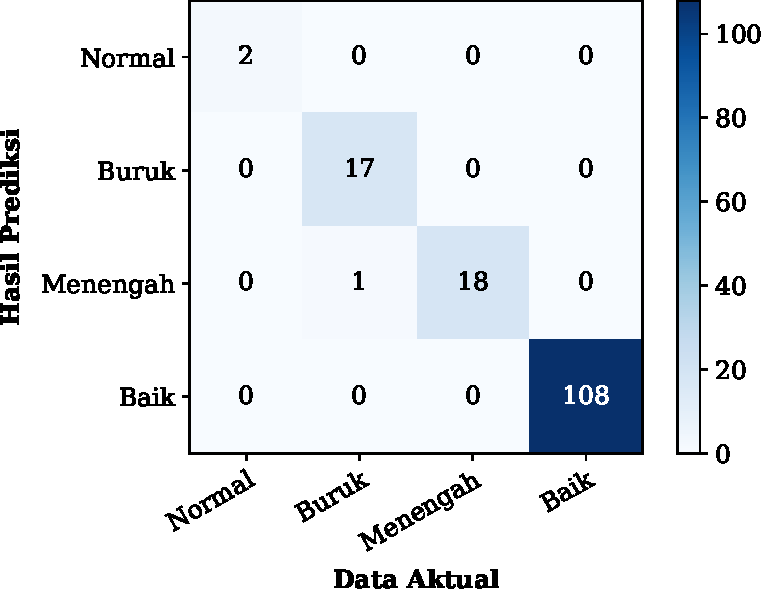
\includegraphics[width=0.6\textwidth]{BAB-4/plot/CM_rasio_data_besar.pdf}	
		\captionof{figure}{Studi Kasus 1: \textit{Confusion Matrix} Percobaan Menggunakan Rasio Data Pelatihan dan Pengujian 8:2}
		\label{gambar:CM rasio layer DS-1}
	\end{minipage}
}
Berdasarkan tampilan pada \textit{confusion matrix} diketahui model dapat mendiagnosis indeks kesehatan transformator daya pada kategori "Normal" tanpa adanya kesalahan. Hal ini didukung dengan perolehan nilai presisi dan sensitivitas yang tinggi pada Gambar \ref{gambar:presisi sensitivity rasio data besar}. Dapat diketahui juga hanya terdapat satu kesalahan yakni kategori yang seharusnya "Buruk"  terdiagnosis sebagai "Menengah".

\centerline{\begin{minipage}{\linewidth}
		\centering
		\vspace{12 pt}
		%% Creator: Matplotlib, PGF backend
%%
%% To include the figure in your LaTeX document, write
%%   \input{<filename>.pgf}
%%
%% Make sure the required packages are loaded in your preamble
%%   \usepackage{pgf}
%%
%% Figures using additional raster images can only be included by \input if
%% they are in the same directory as the main LaTeX file. For loading figures
%% from other directories you can use the `import` package
%%   \usepackage{import}
%%
%% and then include the figures with
%%   \import{<path to file>}{<filename>.pgf}
%%
%% Matplotlib used the following preamble
%%
\begingroup%
\makeatletter%
\begin{pgfpicture}%
\pgfpathrectangle{\pgfpointorigin}{\pgfqpoint{5.640000in}{3.140000in}}%
\pgfusepath{use as bounding box, clip}%
\begin{pgfscope}%
\pgfsetbuttcap%
\pgfsetmiterjoin%
\pgfsetlinewidth{0.000000pt}%
\definecolor{currentstroke}{rgb}{1.000000,1.000000,1.000000}%
\pgfsetstrokecolor{currentstroke}%
\pgfsetstrokeopacity{0.000000}%
\pgfsetdash{}{0pt}%
\pgfpathmoveto{\pgfqpoint{0.000000in}{0.000000in}}%
\pgfpathlineto{\pgfqpoint{5.640000in}{0.000000in}}%
\pgfpathlineto{\pgfqpoint{5.640000in}{3.140000in}}%
\pgfpathlineto{\pgfqpoint{0.000000in}{3.140000in}}%
\pgfpathclose%
\pgfusepath{}%
\end{pgfscope}%
\begin{pgfscope}%
\pgfsetbuttcap%
\pgfsetmiterjoin%
\definecolor{currentfill}{rgb}{1.000000,1.000000,1.000000}%
\pgfsetfillcolor{currentfill}%
\pgfsetlinewidth{0.000000pt}%
\definecolor{currentstroke}{rgb}{0.000000,0.000000,0.000000}%
\pgfsetstrokecolor{currentstroke}%
\pgfsetstrokeopacity{0.000000}%
\pgfsetdash{}{0pt}%
\pgfpathmoveto{\pgfqpoint{0.523149in}{0.693723in}}%
\pgfpathlineto{\pgfqpoint{2.730000in}{0.693723in}}%
\pgfpathlineto{\pgfqpoint{2.730000in}{3.091775in}}%
\pgfpathlineto{\pgfqpoint{0.523149in}{3.091775in}}%
\pgfpathclose%
\pgfusepath{fill}%
\end{pgfscope}%
\begin{pgfscope}%
\pgfpathrectangle{\pgfqpoint{0.523149in}{0.693723in}}{\pgfqpoint{2.206851in}{2.398052in}}%
\pgfusepath{clip}%
\pgfsetbuttcap%
\pgfsetmiterjoin%
\definecolor{currentfill}{rgb}{0.121569,0.466667,0.705882}%
\pgfsetfillcolor{currentfill}%
\pgfsetlinewidth{0.000000pt}%
\definecolor{currentstroke}{rgb}{0.000000,0.000000,0.000000}%
\pgfsetstrokecolor{currentstroke}%
\pgfsetstrokeopacity{0.000000}%
\pgfsetdash{}{0pt}%
\pgfpathmoveto{\pgfqpoint{0.623460in}{-6.980044in}}%
\pgfpathlineto{\pgfqpoint{0.859487in}{-6.980044in}}%
\pgfpathlineto{\pgfqpoint{0.859487in}{2.612164in}}%
\pgfpathlineto{\pgfqpoint{0.623460in}{2.612164in}}%
\pgfpathclose%
\pgfusepath{fill}%
\end{pgfscope}%
\begin{pgfscope}%
\pgfpathrectangle{\pgfqpoint{0.523149in}{0.693723in}}{\pgfqpoint{2.206851in}{2.398052in}}%
\pgfusepath{clip}%
\pgfsetbuttcap%
\pgfsetmiterjoin%
\definecolor{currentfill}{rgb}{0.121569,0.466667,0.705882}%
\pgfsetfillcolor{currentfill}%
\pgfsetlinewidth{0.000000pt}%
\definecolor{currentstroke}{rgb}{0.000000,0.000000,0.000000}%
\pgfsetstrokecolor{currentstroke}%
\pgfsetstrokeopacity{0.000000}%
\pgfsetdash{}{0pt}%
\pgfpathmoveto{\pgfqpoint{1.213527in}{-6.980044in}}%
\pgfpathlineto{\pgfqpoint{1.449554in}{-6.980044in}}%
\pgfpathlineto{\pgfqpoint{1.449554in}{2.612164in}}%
\pgfpathlineto{\pgfqpoint{1.213527in}{2.612164in}}%
\pgfpathclose%
\pgfusepath{fill}%
\end{pgfscope}%
\begin{pgfscope}%
\pgfpathrectangle{\pgfqpoint{0.523149in}{0.693723in}}{\pgfqpoint{2.206851in}{2.398052in}}%
\pgfusepath{clip}%
\pgfsetbuttcap%
\pgfsetmiterjoin%
\definecolor{currentfill}{rgb}{0.121569,0.466667,0.705882}%
\pgfsetfillcolor{currentfill}%
\pgfsetlinewidth{0.000000pt}%
\definecolor{currentstroke}{rgb}{0.000000,0.000000,0.000000}%
\pgfsetstrokecolor{currentstroke}%
\pgfsetstrokeopacity{0.000000}%
\pgfsetdash{}{0pt}%
\pgfpathmoveto{\pgfqpoint{1.803595in}{-6.980044in}}%
\pgfpathlineto{\pgfqpoint{2.039621in}{-6.980044in}}%
\pgfpathlineto{\pgfqpoint{2.039621in}{2.103777in}}%
\pgfpathlineto{\pgfqpoint{1.803595in}{2.103777in}}%
\pgfpathclose%
\pgfusepath{fill}%
\end{pgfscope}%
\begin{pgfscope}%
\pgfpathrectangle{\pgfqpoint{0.523149in}{0.693723in}}{\pgfqpoint{2.206851in}{2.398052in}}%
\pgfusepath{clip}%
\pgfsetbuttcap%
\pgfsetmiterjoin%
\definecolor{currentfill}{rgb}{0.121569,0.466667,0.705882}%
\pgfsetfillcolor{currentfill}%
\pgfsetlinewidth{0.000000pt}%
\definecolor{currentstroke}{rgb}{0.000000,0.000000,0.000000}%
\pgfsetstrokecolor{currentstroke}%
\pgfsetstrokeopacity{0.000000}%
\pgfsetdash{}{0pt}%
\pgfpathmoveto{\pgfqpoint{2.393662in}{-6.980044in}}%
\pgfpathlineto{\pgfqpoint{2.629689in}{-6.980044in}}%
\pgfpathlineto{\pgfqpoint{2.629689in}{2.612164in}}%
\pgfpathlineto{\pgfqpoint{2.393662in}{2.612164in}}%
\pgfpathclose%
\pgfusepath{fill}%
\end{pgfscope}%
\begin{pgfscope}%
\pgfsetbuttcap%
\pgfsetroundjoin%
\definecolor{currentfill}{rgb}{0.000000,0.000000,0.000000}%
\pgfsetfillcolor{currentfill}%
\pgfsetlinewidth{0.803000pt}%
\definecolor{currentstroke}{rgb}{0.000000,0.000000,0.000000}%
\pgfsetstrokecolor{currentstroke}%
\pgfsetdash{}{0pt}%
\pgfsys@defobject{currentmarker}{\pgfqpoint{0.000000in}{-0.048611in}}{\pgfqpoint{0.000000in}{0.000000in}}{%
\pgfpathmoveto{\pgfqpoint{0.000000in}{0.000000in}}%
\pgfpathlineto{\pgfqpoint{0.000000in}{-0.048611in}}%
\pgfusepath{stroke,fill}%
}%
\begin{pgfscope}%
\pgfsys@transformshift{0.741474in}{0.693723in}%
\pgfsys@useobject{currentmarker}{}%
\end{pgfscope}%
\end{pgfscope}%
\begin{pgfscope}%
\definecolor{textcolor}{rgb}{0.000000,0.000000,0.000000}%
\pgfsetstrokecolor{textcolor}%
\pgfsetfillcolor{textcolor}%
\pgftext[x=0.741474in,y=0.596500in,right,top,rotate=30.000000]{\color{textcolor}\rmfamily\fontsize{10.000000}{12.000000}\selectfont Normal}%
\end{pgfscope}%
\begin{pgfscope}%
\pgfsetbuttcap%
\pgfsetroundjoin%
\definecolor{currentfill}{rgb}{0.000000,0.000000,0.000000}%
\pgfsetfillcolor{currentfill}%
\pgfsetlinewidth{0.803000pt}%
\definecolor{currentstroke}{rgb}{0.000000,0.000000,0.000000}%
\pgfsetstrokecolor{currentstroke}%
\pgfsetdash{}{0pt}%
\pgfsys@defobject{currentmarker}{\pgfqpoint{0.000000in}{-0.048611in}}{\pgfqpoint{0.000000in}{0.000000in}}{%
\pgfpathmoveto{\pgfqpoint{0.000000in}{0.000000in}}%
\pgfpathlineto{\pgfqpoint{0.000000in}{-0.048611in}}%
\pgfusepath{stroke,fill}%
}%
\begin{pgfscope}%
\pgfsys@transformshift{1.331541in}{0.693723in}%
\pgfsys@useobject{currentmarker}{}%
\end{pgfscope}%
\end{pgfscope}%
\begin{pgfscope}%
\definecolor{textcolor}{rgb}{0.000000,0.000000,0.000000}%
\pgfsetstrokecolor{textcolor}%
\pgfsetfillcolor{textcolor}%
\pgftext[x=1.331541in,y=0.596500in,right,top,rotate=30.000000]{\color{textcolor}\rmfamily\fontsize{10.000000}{12.000000}\selectfont Buruk}%
\end{pgfscope}%
\begin{pgfscope}%
\pgfsetbuttcap%
\pgfsetroundjoin%
\definecolor{currentfill}{rgb}{0.000000,0.000000,0.000000}%
\pgfsetfillcolor{currentfill}%
\pgfsetlinewidth{0.803000pt}%
\definecolor{currentstroke}{rgb}{0.000000,0.000000,0.000000}%
\pgfsetstrokecolor{currentstroke}%
\pgfsetdash{}{0pt}%
\pgfsys@defobject{currentmarker}{\pgfqpoint{0.000000in}{-0.048611in}}{\pgfqpoint{0.000000in}{0.000000in}}{%
\pgfpathmoveto{\pgfqpoint{0.000000in}{0.000000in}}%
\pgfpathlineto{\pgfqpoint{0.000000in}{-0.048611in}}%
\pgfusepath{stroke,fill}%
}%
\begin{pgfscope}%
\pgfsys@transformshift{1.921608in}{0.693723in}%
\pgfsys@useobject{currentmarker}{}%
\end{pgfscope}%
\end{pgfscope}%
\begin{pgfscope}%
\definecolor{textcolor}{rgb}{0.000000,0.000000,0.000000}%
\pgfsetstrokecolor{textcolor}%
\pgfsetfillcolor{textcolor}%
\pgftext[x=1.921608in,y=0.596500in,right,top,rotate=30.000000]{\color{textcolor}\rmfamily\fontsize{10.000000}{12.000000}\selectfont Menengah}%
\end{pgfscope}%
\begin{pgfscope}%
\pgfsetbuttcap%
\pgfsetroundjoin%
\definecolor{currentfill}{rgb}{0.000000,0.000000,0.000000}%
\pgfsetfillcolor{currentfill}%
\pgfsetlinewidth{0.803000pt}%
\definecolor{currentstroke}{rgb}{0.000000,0.000000,0.000000}%
\pgfsetstrokecolor{currentstroke}%
\pgfsetdash{}{0pt}%
\pgfsys@defobject{currentmarker}{\pgfqpoint{0.000000in}{-0.048611in}}{\pgfqpoint{0.000000in}{0.000000in}}{%
\pgfpathmoveto{\pgfqpoint{0.000000in}{0.000000in}}%
\pgfpathlineto{\pgfqpoint{0.000000in}{-0.048611in}}%
\pgfusepath{stroke,fill}%
}%
\begin{pgfscope}%
\pgfsys@transformshift{2.511675in}{0.693723in}%
\pgfsys@useobject{currentmarker}{}%
\end{pgfscope}%
\end{pgfscope}%
\begin{pgfscope}%
\definecolor{textcolor}{rgb}{0.000000,0.000000,0.000000}%
\pgfsetstrokecolor{textcolor}%
\pgfsetfillcolor{textcolor}%
\pgftext[x=2.511675in,y=0.596500in,right,top,rotate=30.000000]{\color{textcolor}\rmfamily\fontsize{10.000000}{12.000000}\selectfont Baik}%
\end{pgfscope}%
\begin{pgfscope}%
\definecolor{textcolor}{rgb}{0.000000,0.000000,0.000000}%
\pgfsetstrokecolor{textcolor}%
\pgfsetfillcolor{textcolor}%
\pgftext[x=1.626574in,y=0.123457in,,top]{\color{textcolor}\rmfamily\fontsize{10.000000}{12.000000}\selectfont Kategori}%
\end{pgfscope}%
\begin{pgfscope}%
\pgfsetbuttcap%
\pgfsetroundjoin%
\definecolor{currentfill}{rgb}{0.000000,0.000000,0.000000}%
\pgfsetfillcolor{currentfill}%
\pgfsetlinewidth{0.803000pt}%
\definecolor{currentstroke}{rgb}{0.000000,0.000000,0.000000}%
\pgfsetstrokecolor{currentstroke}%
\pgfsetdash{}{0pt}%
\pgfsys@defobject{currentmarker}{\pgfqpoint{-0.048611in}{0.000000in}}{\pgfqpoint{-0.000000in}{0.000000in}}{%
\pgfpathmoveto{\pgfqpoint{-0.000000in}{0.000000in}}%
\pgfpathlineto{\pgfqpoint{-0.048611in}{0.000000in}}%
\pgfusepath{stroke,fill}%
}%
\begin{pgfscope}%
\pgfsys@transformshift{0.523149in}{0.693723in}%
\pgfsys@useobject{currentmarker}{}%
\end{pgfscope}%
\end{pgfscope}%
\begin{pgfscope}%
\definecolor{textcolor}{rgb}{0.000000,0.000000,0.000000}%
\pgfsetstrokecolor{textcolor}%
\pgfsetfillcolor{textcolor}%
\pgftext[x=0.179012in, y=0.645497in, left, base]{\color{textcolor}\rmfamily\fontsize{10.000000}{12.000000}\selectfont \(\displaystyle {0.80}\)}%
\end{pgfscope}%
\begin{pgfscope}%
\pgfsetbuttcap%
\pgfsetroundjoin%
\definecolor{currentfill}{rgb}{0.000000,0.000000,0.000000}%
\pgfsetfillcolor{currentfill}%
\pgfsetlinewidth{0.803000pt}%
\definecolor{currentstroke}{rgb}{0.000000,0.000000,0.000000}%
\pgfsetstrokecolor{currentstroke}%
\pgfsetdash{}{0pt}%
\pgfsys@defobject{currentmarker}{\pgfqpoint{-0.048611in}{0.000000in}}{\pgfqpoint{-0.000000in}{0.000000in}}{%
\pgfpathmoveto{\pgfqpoint{-0.000000in}{0.000000in}}%
\pgfpathlineto{\pgfqpoint{-0.048611in}{0.000000in}}%
\pgfusepath{stroke,fill}%
}%
\begin{pgfscope}%
\pgfsys@transformshift{0.523149in}{1.173333in}%
\pgfsys@useobject{currentmarker}{}%
\end{pgfscope}%
\end{pgfscope}%
\begin{pgfscope}%
\definecolor{textcolor}{rgb}{0.000000,0.000000,0.000000}%
\pgfsetstrokecolor{textcolor}%
\pgfsetfillcolor{textcolor}%
\pgftext[x=0.179012in, y=1.125108in, left, base]{\color{textcolor}\rmfamily\fontsize{10.000000}{12.000000}\selectfont \(\displaystyle {0.85}\)}%
\end{pgfscope}%
\begin{pgfscope}%
\pgfsetbuttcap%
\pgfsetroundjoin%
\definecolor{currentfill}{rgb}{0.000000,0.000000,0.000000}%
\pgfsetfillcolor{currentfill}%
\pgfsetlinewidth{0.803000pt}%
\definecolor{currentstroke}{rgb}{0.000000,0.000000,0.000000}%
\pgfsetstrokecolor{currentstroke}%
\pgfsetdash{}{0pt}%
\pgfsys@defobject{currentmarker}{\pgfqpoint{-0.048611in}{0.000000in}}{\pgfqpoint{-0.000000in}{0.000000in}}{%
\pgfpathmoveto{\pgfqpoint{-0.000000in}{0.000000in}}%
\pgfpathlineto{\pgfqpoint{-0.048611in}{0.000000in}}%
\pgfusepath{stroke,fill}%
}%
\begin{pgfscope}%
\pgfsys@transformshift{0.523149in}{1.652944in}%
\pgfsys@useobject{currentmarker}{}%
\end{pgfscope}%
\end{pgfscope}%
\begin{pgfscope}%
\definecolor{textcolor}{rgb}{0.000000,0.000000,0.000000}%
\pgfsetstrokecolor{textcolor}%
\pgfsetfillcolor{textcolor}%
\pgftext[x=0.179012in, y=1.604718in, left, base]{\color{textcolor}\rmfamily\fontsize{10.000000}{12.000000}\selectfont \(\displaystyle {0.90}\)}%
\end{pgfscope}%
\begin{pgfscope}%
\pgfsetbuttcap%
\pgfsetroundjoin%
\definecolor{currentfill}{rgb}{0.000000,0.000000,0.000000}%
\pgfsetfillcolor{currentfill}%
\pgfsetlinewidth{0.803000pt}%
\definecolor{currentstroke}{rgb}{0.000000,0.000000,0.000000}%
\pgfsetstrokecolor{currentstroke}%
\pgfsetdash{}{0pt}%
\pgfsys@defobject{currentmarker}{\pgfqpoint{-0.048611in}{0.000000in}}{\pgfqpoint{-0.000000in}{0.000000in}}{%
\pgfpathmoveto{\pgfqpoint{-0.000000in}{0.000000in}}%
\pgfpathlineto{\pgfqpoint{-0.048611in}{0.000000in}}%
\pgfusepath{stroke,fill}%
}%
\begin{pgfscope}%
\pgfsys@transformshift{0.523149in}{2.132554in}%
\pgfsys@useobject{currentmarker}{}%
\end{pgfscope}%
\end{pgfscope}%
\begin{pgfscope}%
\definecolor{textcolor}{rgb}{0.000000,0.000000,0.000000}%
\pgfsetstrokecolor{textcolor}%
\pgfsetfillcolor{textcolor}%
\pgftext[x=0.179012in, y=2.084329in, left, base]{\color{textcolor}\rmfamily\fontsize{10.000000}{12.000000}\selectfont \(\displaystyle {0.95}\)}%
\end{pgfscope}%
\begin{pgfscope}%
\pgfsetbuttcap%
\pgfsetroundjoin%
\definecolor{currentfill}{rgb}{0.000000,0.000000,0.000000}%
\pgfsetfillcolor{currentfill}%
\pgfsetlinewidth{0.803000pt}%
\definecolor{currentstroke}{rgb}{0.000000,0.000000,0.000000}%
\pgfsetstrokecolor{currentstroke}%
\pgfsetdash{}{0pt}%
\pgfsys@defobject{currentmarker}{\pgfqpoint{-0.048611in}{0.000000in}}{\pgfqpoint{-0.000000in}{0.000000in}}{%
\pgfpathmoveto{\pgfqpoint{-0.000000in}{0.000000in}}%
\pgfpathlineto{\pgfqpoint{-0.048611in}{0.000000in}}%
\pgfusepath{stroke,fill}%
}%
\begin{pgfscope}%
\pgfsys@transformshift{0.523149in}{2.612164in}%
\pgfsys@useobject{currentmarker}{}%
\end{pgfscope}%
\end{pgfscope}%
\begin{pgfscope}%
\definecolor{textcolor}{rgb}{0.000000,0.000000,0.000000}%
\pgfsetstrokecolor{textcolor}%
\pgfsetfillcolor{textcolor}%
\pgftext[x=0.179012in, y=2.563939in, left, base]{\color{textcolor}\rmfamily\fontsize{10.000000}{12.000000}\selectfont \(\displaystyle {1.00}\)}%
\end{pgfscope}%
\begin{pgfscope}%
\pgfsetbuttcap%
\pgfsetroundjoin%
\definecolor{currentfill}{rgb}{0.000000,0.000000,0.000000}%
\pgfsetfillcolor{currentfill}%
\pgfsetlinewidth{0.803000pt}%
\definecolor{currentstroke}{rgb}{0.000000,0.000000,0.000000}%
\pgfsetstrokecolor{currentstroke}%
\pgfsetdash{}{0pt}%
\pgfsys@defobject{currentmarker}{\pgfqpoint{-0.048611in}{0.000000in}}{\pgfqpoint{-0.000000in}{0.000000in}}{%
\pgfpathmoveto{\pgfqpoint{-0.000000in}{0.000000in}}%
\pgfpathlineto{\pgfqpoint{-0.048611in}{0.000000in}}%
\pgfusepath{stroke,fill}%
}%
\begin{pgfscope}%
\pgfsys@transformshift{0.523149in}{3.091775in}%
\pgfsys@useobject{currentmarker}{}%
\end{pgfscope}%
\end{pgfscope}%
\begin{pgfscope}%
\definecolor{textcolor}{rgb}{0.000000,0.000000,0.000000}%
\pgfsetstrokecolor{textcolor}%
\pgfsetfillcolor{textcolor}%
\pgftext[x=0.179012in, y=3.043549in, left, base]{\color{textcolor}\rmfamily\fontsize{10.000000}{12.000000}\selectfont \(\displaystyle {1.05}\)}%
\end{pgfscope}%
\begin{pgfscope}%
\definecolor{textcolor}{rgb}{0.000000,0.000000,0.000000}%
\pgfsetstrokecolor{textcolor}%
\pgfsetfillcolor{textcolor}%
\pgftext[x=0.123457in,y=1.892749in,,bottom,rotate=90.000000]{\color{textcolor}\rmfamily\fontsize{10.000000}{12.000000}\selectfont Presisi}%
\end{pgfscope}%
\begin{pgfscope}%
\pgfsetrectcap%
\pgfsetmiterjoin%
\pgfsetlinewidth{0.803000pt}%
\definecolor{currentstroke}{rgb}{0.000000,0.000000,0.000000}%
\pgfsetstrokecolor{currentstroke}%
\pgfsetdash{}{0pt}%
\pgfpathmoveto{\pgfqpoint{0.523149in}{0.693723in}}%
\pgfpathlineto{\pgfqpoint{0.523149in}{3.091775in}}%
\pgfusepath{stroke}%
\end{pgfscope}%
\begin{pgfscope}%
\pgfsetrectcap%
\pgfsetmiterjoin%
\pgfsetlinewidth{0.803000pt}%
\definecolor{currentstroke}{rgb}{0.000000,0.000000,0.000000}%
\pgfsetstrokecolor{currentstroke}%
\pgfsetdash{}{0pt}%
\pgfpathmoveto{\pgfqpoint{2.730000in}{0.693723in}}%
\pgfpathlineto{\pgfqpoint{2.730000in}{3.091775in}}%
\pgfusepath{stroke}%
\end{pgfscope}%
\begin{pgfscope}%
\pgfsetrectcap%
\pgfsetmiterjoin%
\pgfsetlinewidth{0.803000pt}%
\definecolor{currentstroke}{rgb}{0.000000,0.000000,0.000000}%
\pgfsetstrokecolor{currentstroke}%
\pgfsetdash{}{0pt}%
\pgfpathmoveto{\pgfqpoint{0.523149in}{0.693723in}}%
\pgfpathlineto{\pgfqpoint{2.730000in}{0.693723in}}%
\pgfusepath{stroke}%
\end{pgfscope}%
\begin{pgfscope}%
\pgfsetrectcap%
\pgfsetmiterjoin%
\pgfsetlinewidth{0.803000pt}%
\definecolor{currentstroke}{rgb}{0.000000,0.000000,0.000000}%
\pgfsetstrokecolor{currentstroke}%
\pgfsetdash{}{0pt}%
\pgfpathmoveto{\pgfqpoint{0.523149in}{3.091775in}}%
\pgfpathlineto{\pgfqpoint{2.730000in}{3.091775in}}%
\pgfusepath{stroke}%
\end{pgfscope}%
\begin{pgfscope}%
\definecolor{textcolor}{rgb}{0.000000,0.000000,0.000000}%
\pgfsetstrokecolor{textcolor}%
\pgfsetfillcolor{textcolor}%
\pgftext[x=0.741474in,y=2.708086in,,bottom]{\color{textcolor}\rmfamily\fontsize{9.000000}{10.800000}\selectfont 1.0}%
\end{pgfscope}%
\begin{pgfscope}%
\definecolor{textcolor}{rgb}{0.000000,0.000000,0.000000}%
\pgfsetstrokecolor{textcolor}%
\pgfsetfillcolor{textcolor}%
\pgftext[x=1.331541in,y=2.708086in,,bottom]{\color{textcolor}\rmfamily\fontsize{9.000000}{10.800000}\selectfont 1.0}%
\end{pgfscope}%
\begin{pgfscope}%
\definecolor{textcolor}{rgb}{0.000000,0.000000,0.000000}%
\pgfsetstrokecolor{textcolor}%
\pgfsetfillcolor{textcolor}%
\pgftext[x=1.921608in,y=2.199699in,,bottom]{\color{textcolor}\rmfamily\fontsize{9.000000}{10.800000}\selectfont 0.947}%
\end{pgfscope}%
\begin{pgfscope}%
\definecolor{textcolor}{rgb}{0.000000,0.000000,0.000000}%
\pgfsetstrokecolor{textcolor}%
\pgfsetfillcolor{textcolor}%
\pgftext[x=2.511675in,y=2.708086in,,bottom]{\color{textcolor}\rmfamily\fontsize{9.000000}{10.800000}\selectfont 1.0}%
\end{pgfscope}%
\begin{pgfscope}%
\pgfsetbuttcap%
\pgfsetmiterjoin%
\definecolor{currentfill}{rgb}{1.000000,1.000000,1.000000}%
\pgfsetfillcolor{currentfill}%
\pgfsetlinewidth{0.000000pt}%
\definecolor{currentstroke}{rgb}{0.000000,0.000000,0.000000}%
\pgfsetstrokecolor{currentstroke}%
\pgfsetstrokeopacity{0.000000}%
\pgfsetdash{}{0pt}%
\pgfpathmoveto{\pgfqpoint{3.433149in}{0.693723in}}%
\pgfpathlineto{\pgfqpoint{5.640000in}{0.693723in}}%
\pgfpathlineto{\pgfqpoint{5.640000in}{3.091775in}}%
\pgfpathlineto{\pgfqpoint{3.433149in}{3.091775in}}%
\pgfpathclose%
\pgfusepath{fill}%
\end{pgfscope}%
\begin{pgfscope}%
\pgfpathrectangle{\pgfqpoint{3.433149in}{0.693723in}}{\pgfqpoint{2.206851in}{2.398052in}}%
\pgfusepath{clip}%
\pgfsetbuttcap%
\pgfsetmiterjoin%
\definecolor{currentfill}{rgb}{1.000000,0.498039,0.054902}%
\pgfsetfillcolor{currentfill}%
\pgfsetlinewidth{0.000000pt}%
\definecolor{currentstroke}{rgb}{0.000000,0.000000,0.000000}%
\pgfsetstrokecolor{currentstroke}%
\pgfsetstrokeopacity{0.000000}%
\pgfsetdash{}{0pt}%
\pgfpathmoveto{\pgfqpoint{3.533460in}{-6.980044in}}%
\pgfpathlineto{\pgfqpoint{3.769487in}{-6.980044in}}%
\pgfpathlineto{\pgfqpoint{3.769487in}{2.612164in}}%
\pgfpathlineto{\pgfqpoint{3.533460in}{2.612164in}}%
\pgfpathclose%
\pgfusepath{fill}%
\end{pgfscope}%
\begin{pgfscope}%
\pgfpathrectangle{\pgfqpoint{3.433149in}{0.693723in}}{\pgfqpoint{2.206851in}{2.398052in}}%
\pgfusepath{clip}%
\pgfsetbuttcap%
\pgfsetmiterjoin%
\definecolor{currentfill}{rgb}{1.000000,0.498039,0.054902}%
\pgfsetfillcolor{currentfill}%
\pgfsetlinewidth{0.000000pt}%
\definecolor{currentstroke}{rgb}{0.000000,0.000000,0.000000}%
\pgfsetstrokecolor{currentstroke}%
\pgfsetstrokeopacity{0.000000}%
\pgfsetdash{}{0pt}%
\pgfpathmoveto{\pgfqpoint{4.123527in}{-6.980044in}}%
\pgfpathlineto{\pgfqpoint{4.359554in}{-6.980044in}}%
\pgfpathlineto{\pgfqpoint{4.359554in}{2.075001in}}%
\pgfpathlineto{\pgfqpoint{4.123527in}{2.075001in}}%
\pgfpathclose%
\pgfusepath{fill}%
\end{pgfscope}%
\begin{pgfscope}%
\pgfpathrectangle{\pgfqpoint{3.433149in}{0.693723in}}{\pgfqpoint{2.206851in}{2.398052in}}%
\pgfusepath{clip}%
\pgfsetbuttcap%
\pgfsetmiterjoin%
\definecolor{currentfill}{rgb}{1.000000,0.498039,0.054902}%
\pgfsetfillcolor{currentfill}%
\pgfsetlinewidth{0.000000pt}%
\definecolor{currentstroke}{rgb}{0.000000,0.000000,0.000000}%
\pgfsetstrokecolor{currentstroke}%
\pgfsetstrokeopacity{0.000000}%
\pgfsetdash{}{0pt}%
\pgfpathmoveto{\pgfqpoint{4.713595in}{-6.980044in}}%
\pgfpathlineto{\pgfqpoint{4.949621in}{-6.980044in}}%
\pgfpathlineto{\pgfqpoint{4.949621in}{2.612164in}}%
\pgfpathlineto{\pgfqpoint{4.713595in}{2.612164in}}%
\pgfpathclose%
\pgfusepath{fill}%
\end{pgfscope}%
\begin{pgfscope}%
\pgfpathrectangle{\pgfqpoint{3.433149in}{0.693723in}}{\pgfqpoint{2.206851in}{2.398052in}}%
\pgfusepath{clip}%
\pgfsetbuttcap%
\pgfsetmiterjoin%
\definecolor{currentfill}{rgb}{1.000000,0.498039,0.054902}%
\pgfsetfillcolor{currentfill}%
\pgfsetlinewidth{0.000000pt}%
\definecolor{currentstroke}{rgb}{0.000000,0.000000,0.000000}%
\pgfsetstrokecolor{currentstroke}%
\pgfsetstrokeopacity{0.000000}%
\pgfsetdash{}{0pt}%
\pgfpathmoveto{\pgfqpoint{5.303662in}{-6.980044in}}%
\pgfpathlineto{\pgfqpoint{5.539689in}{-6.980044in}}%
\pgfpathlineto{\pgfqpoint{5.539689in}{2.612164in}}%
\pgfpathlineto{\pgfqpoint{5.303662in}{2.612164in}}%
\pgfpathclose%
\pgfusepath{fill}%
\end{pgfscope}%
\begin{pgfscope}%
\pgfsetbuttcap%
\pgfsetroundjoin%
\definecolor{currentfill}{rgb}{0.000000,0.000000,0.000000}%
\pgfsetfillcolor{currentfill}%
\pgfsetlinewidth{0.803000pt}%
\definecolor{currentstroke}{rgb}{0.000000,0.000000,0.000000}%
\pgfsetstrokecolor{currentstroke}%
\pgfsetdash{}{0pt}%
\pgfsys@defobject{currentmarker}{\pgfqpoint{0.000000in}{-0.048611in}}{\pgfqpoint{0.000000in}{0.000000in}}{%
\pgfpathmoveto{\pgfqpoint{0.000000in}{0.000000in}}%
\pgfpathlineto{\pgfqpoint{0.000000in}{-0.048611in}}%
\pgfusepath{stroke,fill}%
}%
\begin{pgfscope}%
\pgfsys@transformshift{3.651474in}{0.693723in}%
\pgfsys@useobject{currentmarker}{}%
\end{pgfscope}%
\end{pgfscope}%
\begin{pgfscope}%
\definecolor{textcolor}{rgb}{0.000000,0.000000,0.000000}%
\pgfsetstrokecolor{textcolor}%
\pgfsetfillcolor{textcolor}%
\pgftext[x=3.651474in,y=0.596500in,right,top,rotate=30.000000]{\color{textcolor}\rmfamily\fontsize{10.000000}{12.000000}\selectfont Normal}%
\end{pgfscope}%
\begin{pgfscope}%
\pgfsetbuttcap%
\pgfsetroundjoin%
\definecolor{currentfill}{rgb}{0.000000,0.000000,0.000000}%
\pgfsetfillcolor{currentfill}%
\pgfsetlinewidth{0.803000pt}%
\definecolor{currentstroke}{rgb}{0.000000,0.000000,0.000000}%
\pgfsetstrokecolor{currentstroke}%
\pgfsetdash{}{0pt}%
\pgfsys@defobject{currentmarker}{\pgfqpoint{0.000000in}{-0.048611in}}{\pgfqpoint{0.000000in}{0.000000in}}{%
\pgfpathmoveto{\pgfqpoint{0.000000in}{0.000000in}}%
\pgfpathlineto{\pgfqpoint{0.000000in}{-0.048611in}}%
\pgfusepath{stroke,fill}%
}%
\begin{pgfscope}%
\pgfsys@transformshift{4.241541in}{0.693723in}%
\pgfsys@useobject{currentmarker}{}%
\end{pgfscope}%
\end{pgfscope}%
\begin{pgfscope}%
\definecolor{textcolor}{rgb}{0.000000,0.000000,0.000000}%
\pgfsetstrokecolor{textcolor}%
\pgfsetfillcolor{textcolor}%
\pgftext[x=4.241541in,y=0.596500in,right,top,rotate=30.000000]{\color{textcolor}\rmfamily\fontsize{10.000000}{12.000000}\selectfont Buruk}%
\end{pgfscope}%
\begin{pgfscope}%
\pgfsetbuttcap%
\pgfsetroundjoin%
\definecolor{currentfill}{rgb}{0.000000,0.000000,0.000000}%
\pgfsetfillcolor{currentfill}%
\pgfsetlinewidth{0.803000pt}%
\definecolor{currentstroke}{rgb}{0.000000,0.000000,0.000000}%
\pgfsetstrokecolor{currentstroke}%
\pgfsetdash{}{0pt}%
\pgfsys@defobject{currentmarker}{\pgfqpoint{0.000000in}{-0.048611in}}{\pgfqpoint{0.000000in}{0.000000in}}{%
\pgfpathmoveto{\pgfqpoint{0.000000in}{0.000000in}}%
\pgfpathlineto{\pgfqpoint{0.000000in}{-0.048611in}}%
\pgfusepath{stroke,fill}%
}%
\begin{pgfscope}%
\pgfsys@transformshift{4.831608in}{0.693723in}%
\pgfsys@useobject{currentmarker}{}%
\end{pgfscope}%
\end{pgfscope}%
\begin{pgfscope}%
\definecolor{textcolor}{rgb}{0.000000,0.000000,0.000000}%
\pgfsetstrokecolor{textcolor}%
\pgfsetfillcolor{textcolor}%
\pgftext[x=4.831608in,y=0.596500in,right,top,rotate=30.000000]{\color{textcolor}\rmfamily\fontsize{10.000000}{12.000000}\selectfont Menengah}%
\end{pgfscope}%
\begin{pgfscope}%
\pgfsetbuttcap%
\pgfsetroundjoin%
\definecolor{currentfill}{rgb}{0.000000,0.000000,0.000000}%
\pgfsetfillcolor{currentfill}%
\pgfsetlinewidth{0.803000pt}%
\definecolor{currentstroke}{rgb}{0.000000,0.000000,0.000000}%
\pgfsetstrokecolor{currentstroke}%
\pgfsetdash{}{0pt}%
\pgfsys@defobject{currentmarker}{\pgfqpoint{0.000000in}{-0.048611in}}{\pgfqpoint{0.000000in}{0.000000in}}{%
\pgfpathmoveto{\pgfqpoint{0.000000in}{0.000000in}}%
\pgfpathlineto{\pgfqpoint{0.000000in}{-0.048611in}}%
\pgfusepath{stroke,fill}%
}%
\begin{pgfscope}%
\pgfsys@transformshift{5.421675in}{0.693723in}%
\pgfsys@useobject{currentmarker}{}%
\end{pgfscope}%
\end{pgfscope}%
\begin{pgfscope}%
\definecolor{textcolor}{rgb}{0.000000,0.000000,0.000000}%
\pgfsetstrokecolor{textcolor}%
\pgfsetfillcolor{textcolor}%
\pgftext[x=5.421675in,y=0.596500in,right,top,rotate=30.000000]{\color{textcolor}\rmfamily\fontsize{10.000000}{12.000000}\selectfont Baik}%
\end{pgfscope}%
\begin{pgfscope}%
\definecolor{textcolor}{rgb}{0.000000,0.000000,0.000000}%
\pgfsetstrokecolor{textcolor}%
\pgfsetfillcolor{textcolor}%
\pgftext[x=4.536574in,y=0.123457in,,top]{\color{textcolor}\rmfamily\fontsize{10.000000}{12.000000}\selectfont Kategori}%
\end{pgfscope}%
\begin{pgfscope}%
\pgfsetbuttcap%
\pgfsetroundjoin%
\definecolor{currentfill}{rgb}{0.000000,0.000000,0.000000}%
\pgfsetfillcolor{currentfill}%
\pgfsetlinewidth{0.803000pt}%
\definecolor{currentstroke}{rgb}{0.000000,0.000000,0.000000}%
\pgfsetstrokecolor{currentstroke}%
\pgfsetdash{}{0pt}%
\pgfsys@defobject{currentmarker}{\pgfqpoint{-0.048611in}{0.000000in}}{\pgfqpoint{-0.000000in}{0.000000in}}{%
\pgfpathmoveto{\pgfqpoint{-0.000000in}{0.000000in}}%
\pgfpathlineto{\pgfqpoint{-0.048611in}{0.000000in}}%
\pgfusepath{stroke,fill}%
}%
\begin{pgfscope}%
\pgfsys@transformshift{3.433149in}{0.693723in}%
\pgfsys@useobject{currentmarker}{}%
\end{pgfscope}%
\end{pgfscope}%
\begin{pgfscope}%
\definecolor{textcolor}{rgb}{0.000000,0.000000,0.000000}%
\pgfsetstrokecolor{textcolor}%
\pgfsetfillcolor{textcolor}%
\pgftext[x=3.089012in, y=0.645497in, left, base]{\color{textcolor}\rmfamily\fontsize{10.000000}{12.000000}\selectfont \(\displaystyle {0.80}\)}%
\end{pgfscope}%
\begin{pgfscope}%
\pgfsetbuttcap%
\pgfsetroundjoin%
\definecolor{currentfill}{rgb}{0.000000,0.000000,0.000000}%
\pgfsetfillcolor{currentfill}%
\pgfsetlinewidth{0.803000pt}%
\definecolor{currentstroke}{rgb}{0.000000,0.000000,0.000000}%
\pgfsetstrokecolor{currentstroke}%
\pgfsetdash{}{0pt}%
\pgfsys@defobject{currentmarker}{\pgfqpoint{-0.048611in}{0.000000in}}{\pgfqpoint{-0.000000in}{0.000000in}}{%
\pgfpathmoveto{\pgfqpoint{-0.000000in}{0.000000in}}%
\pgfpathlineto{\pgfqpoint{-0.048611in}{0.000000in}}%
\pgfusepath{stroke,fill}%
}%
\begin{pgfscope}%
\pgfsys@transformshift{3.433149in}{1.173333in}%
\pgfsys@useobject{currentmarker}{}%
\end{pgfscope}%
\end{pgfscope}%
\begin{pgfscope}%
\definecolor{textcolor}{rgb}{0.000000,0.000000,0.000000}%
\pgfsetstrokecolor{textcolor}%
\pgfsetfillcolor{textcolor}%
\pgftext[x=3.089012in, y=1.125108in, left, base]{\color{textcolor}\rmfamily\fontsize{10.000000}{12.000000}\selectfont \(\displaystyle {0.85}\)}%
\end{pgfscope}%
\begin{pgfscope}%
\pgfsetbuttcap%
\pgfsetroundjoin%
\definecolor{currentfill}{rgb}{0.000000,0.000000,0.000000}%
\pgfsetfillcolor{currentfill}%
\pgfsetlinewidth{0.803000pt}%
\definecolor{currentstroke}{rgb}{0.000000,0.000000,0.000000}%
\pgfsetstrokecolor{currentstroke}%
\pgfsetdash{}{0pt}%
\pgfsys@defobject{currentmarker}{\pgfqpoint{-0.048611in}{0.000000in}}{\pgfqpoint{-0.000000in}{0.000000in}}{%
\pgfpathmoveto{\pgfqpoint{-0.000000in}{0.000000in}}%
\pgfpathlineto{\pgfqpoint{-0.048611in}{0.000000in}}%
\pgfusepath{stroke,fill}%
}%
\begin{pgfscope}%
\pgfsys@transformshift{3.433149in}{1.652944in}%
\pgfsys@useobject{currentmarker}{}%
\end{pgfscope}%
\end{pgfscope}%
\begin{pgfscope}%
\definecolor{textcolor}{rgb}{0.000000,0.000000,0.000000}%
\pgfsetstrokecolor{textcolor}%
\pgfsetfillcolor{textcolor}%
\pgftext[x=3.089012in, y=1.604718in, left, base]{\color{textcolor}\rmfamily\fontsize{10.000000}{12.000000}\selectfont \(\displaystyle {0.90}\)}%
\end{pgfscope}%
\begin{pgfscope}%
\pgfsetbuttcap%
\pgfsetroundjoin%
\definecolor{currentfill}{rgb}{0.000000,0.000000,0.000000}%
\pgfsetfillcolor{currentfill}%
\pgfsetlinewidth{0.803000pt}%
\definecolor{currentstroke}{rgb}{0.000000,0.000000,0.000000}%
\pgfsetstrokecolor{currentstroke}%
\pgfsetdash{}{0pt}%
\pgfsys@defobject{currentmarker}{\pgfqpoint{-0.048611in}{0.000000in}}{\pgfqpoint{-0.000000in}{0.000000in}}{%
\pgfpathmoveto{\pgfqpoint{-0.000000in}{0.000000in}}%
\pgfpathlineto{\pgfqpoint{-0.048611in}{0.000000in}}%
\pgfusepath{stroke,fill}%
}%
\begin{pgfscope}%
\pgfsys@transformshift{3.433149in}{2.132554in}%
\pgfsys@useobject{currentmarker}{}%
\end{pgfscope}%
\end{pgfscope}%
\begin{pgfscope}%
\definecolor{textcolor}{rgb}{0.000000,0.000000,0.000000}%
\pgfsetstrokecolor{textcolor}%
\pgfsetfillcolor{textcolor}%
\pgftext[x=3.089012in, y=2.084329in, left, base]{\color{textcolor}\rmfamily\fontsize{10.000000}{12.000000}\selectfont \(\displaystyle {0.95}\)}%
\end{pgfscope}%
\begin{pgfscope}%
\pgfsetbuttcap%
\pgfsetroundjoin%
\definecolor{currentfill}{rgb}{0.000000,0.000000,0.000000}%
\pgfsetfillcolor{currentfill}%
\pgfsetlinewidth{0.803000pt}%
\definecolor{currentstroke}{rgb}{0.000000,0.000000,0.000000}%
\pgfsetstrokecolor{currentstroke}%
\pgfsetdash{}{0pt}%
\pgfsys@defobject{currentmarker}{\pgfqpoint{-0.048611in}{0.000000in}}{\pgfqpoint{-0.000000in}{0.000000in}}{%
\pgfpathmoveto{\pgfqpoint{-0.000000in}{0.000000in}}%
\pgfpathlineto{\pgfqpoint{-0.048611in}{0.000000in}}%
\pgfusepath{stroke,fill}%
}%
\begin{pgfscope}%
\pgfsys@transformshift{3.433149in}{2.612164in}%
\pgfsys@useobject{currentmarker}{}%
\end{pgfscope}%
\end{pgfscope}%
\begin{pgfscope}%
\definecolor{textcolor}{rgb}{0.000000,0.000000,0.000000}%
\pgfsetstrokecolor{textcolor}%
\pgfsetfillcolor{textcolor}%
\pgftext[x=3.089012in, y=2.563939in, left, base]{\color{textcolor}\rmfamily\fontsize{10.000000}{12.000000}\selectfont \(\displaystyle {1.00}\)}%
\end{pgfscope}%
\begin{pgfscope}%
\pgfsetbuttcap%
\pgfsetroundjoin%
\definecolor{currentfill}{rgb}{0.000000,0.000000,0.000000}%
\pgfsetfillcolor{currentfill}%
\pgfsetlinewidth{0.803000pt}%
\definecolor{currentstroke}{rgb}{0.000000,0.000000,0.000000}%
\pgfsetstrokecolor{currentstroke}%
\pgfsetdash{}{0pt}%
\pgfsys@defobject{currentmarker}{\pgfqpoint{-0.048611in}{0.000000in}}{\pgfqpoint{-0.000000in}{0.000000in}}{%
\pgfpathmoveto{\pgfqpoint{-0.000000in}{0.000000in}}%
\pgfpathlineto{\pgfqpoint{-0.048611in}{0.000000in}}%
\pgfusepath{stroke,fill}%
}%
\begin{pgfscope}%
\pgfsys@transformshift{3.433149in}{3.091775in}%
\pgfsys@useobject{currentmarker}{}%
\end{pgfscope}%
\end{pgfscope}%
\begin{pgfscope}%
\definecolor{textcolor}{rgb}{0.000000,0.000000,0.000000}%
\pgfsetstrokecolor{textcolor}%
\pgfsetfillcolor{textcolor}%
\pgftext[x=3.089012in, y=3.043549in, left, base]{\color{textcolor}\rmfamily\fontsize{10.000000}{12.000000}\selectfont \(\displaystyle {1.05}\)}%
\end{pgfscope}%
\begin{pgfscope}%
\definecolor{textcolor}{rgb}{0.000000,0.000000,0.000000}%
\pgfsetstrokecolor{textcolor}%
\pgfsetfillcolor{textcolor}%
\pgftext[x=3.033457in,y=1.892749in,,bottom,rotate=90.000000]{\color{textcolor}\rmfamily\fontsize{10.000000}{12.000000}\selectfont Sensitivitas}%
\end{pgfscope}%
\begin{pgfscope}%
\pgfsetrectcap%
\pgfsetmiterjoin%
\pgfsetlinewidth{0.803000pt}%
\definecolor{currentstroke}{rgb}{0.000000,0.000000,0.000000}%
\pgfsetstrokecolor{currentstroke}%
\pgfsetdash{}{0pt}%
\pgfpathmoveto{\pgfqpoint{3.433149in}{0.693723in}}%
\pgfpathlineto{\pgfqpoint{3.433149in}{3.091775in}}%
\pgfusepath{stroke}%
\end{pgfscope}%
\begin{pgfscope}%
\pgfsetrectcap%
\pgfsetmiterjoin%
\pgfsetlinewidth{0.803000pt}%
\definecolor{currentstroke}{rgb}{0.000000,0.000000,0.000000}%
\pgfsetstrokecolor{currentstroke}%
\pgfsetdash{}{0pt}%
\pgfpathmoveto{\pgfqpoint{5.640000in}{0.693723in}}%
\pgfpathlineto{\pgfqpoint{5.640000in}{3.091775in}}%
\pgfusepath{stroke}%
\end{pgfscope}%
\begin{pgfscope}%
\pgfsetrectcap%
\pgfsetmiterjoin%
\pgfsetlinewidth{0.803000pt}%
\definecolor{currentstroke}{rgb}{0.000000,0.000000,0.000000}%
\pgfsetstrokecolor{currentstroke}%
\pgfsetdash{}{0pt}%
\pgfpathmoveto{\pgfqpoint{3.433149in}{0.693723in}}%
\pgfpathlineto{\pgfqpoint{5.640000in}{0.693723in}}%
\pgfusepath{stroke}%
\end{pgfscope}%
\begin{pgfscope}%
\pgfsetrectcap%
\pgfsetmiterjoin%
\pgfsetlinewidth{0.803000pt}%
\definecolor{currentstroke}{rgb}{0.000000,0.000000,0.000000}%
\pgfsetstrokecolor{currentstroke}%
\pgfsetdash{}{0pt}%
\pgfpathmoveto{\pgfqpoint{3.433149in}{3.091775in}}%
\pgfpathlineto{\pgfqpoint{5.640000in}{3.091775in}}%
\pgfusepath{stroke}%
\end{pgfscope}%
\begin{pgfscope}%
\definecolor{textcolor}{rgb}{0.000000,0.000000,0.000000}%
\pgfsetstrokecolor{textcolor}%
\pgfsetfillcolor{textcolor}%
\pgftext[x=3.651474in,y=2.708086in,,bottom]{\color{textcolor}\rmfamily\fontsize{9.000000}{10.800000}\selectfont 1.0}%
\end{pgfscope}%
\begin{pgfscope}%
\definecolor{textcolor}{rgb}{0.000000,0.000000,0.000000}%
\pgfsetstrokecolor{textcolor}%
\pgfsetfillcolor{textcolor}%
\pgftext[x=4.241541in,y=2.170923in,,bottom]{\color{textcolor}\rmfamily\fontsize{9.000000}{10.800000}\selectfont 0.944}%
\end{pgfscope}%
\begin{pgfscope}%
\definecolor{textcolor}{rgb}{0.000000,0.000000,0.000000}%
\pgfsetstrokecolor{textcolor}%
\pgfsetfillcolor{textcolor}%
\pgftext[x=4.831608in,y=2.708086in,,bottom]{\color{textcolor}\rmfamily\fontsize{9.000000}{10.800000}\selectfont 1.0}%
\end{pgfscope}%
\begin{pgfscope}%
\definecolor{textcolor}{rgb}{0.000000,0.000000,0.000000}%
\pgfsetstrokecolor{textcolor}%
\pgfsetfillcolor{textcolor}%
\pgftext[x=5.421675in,y=2.708086in,,bottom]{\color{textcolor}\rmfamily\fontsize{9.000000}{10.800000}\selectfont 1.0}%
\end{pgfscope}%
\end{pgfpicture}%
\makeatother%
\endgroup%

		\captionof{figure}{Studi Kasus 1: Presisi dan Sensitivitas Percobaan Menggunakan Rasio Data Pelatihan dan Pengujian 8:2}
		\label{gambar:presisi sensitivity rasio data besar}
\end{minipage}}

Dengan demikian, perubahan jumlah rasio set data dapat mempengaruhi hasil akurasi menjadi lebih baik. Hal ini dapat terjadi karena pada dasarnya terdapat penambahan data pada proses pelatihan sehingga model menjadi lebih mengenali pola data. Dengan Demikian, maka model yang diimplementasikan pada aplikasi ialah model hasil percobaan dengan menggunakan rasio data 8:2 pada pemisahan data pelatihan dan pengujian.

\section{Studi Kasus 2}
\subsection{Perubahan Jumlah \textit{Hidden Layer}}
Pada studi kasus 2 pada dasarnya memiliki mekanisme yang sama terhadap percobaan yang telah dilakukan pada studi kasus 1. Percobaan ini merupakan sebuah langkah lanjutan untuk mengetahui apakah pada penggunaan data yang berbeda dapat digunakan arsitektur yang sama. Telah dijelaskan pada Bab \ref{BAB3:Metode} bahwa percobaan menggunakan set data 2, yang akan dibagi atas data pelatihan dan pengujian dangan rasio 7:3. Percobaan pertama dilakukan yakni melakukan pelatihan terhadap model LSTM dengan variabel bebas yang diubah adalah jumlah \textit{hidden layer} yang digunakan. Jumlah \textit{hidden layer} yang diuji coba terdiri dari penggunaan yang tunggal sampai 5 buah. Pada Gambar \ref{gambar:perbandingan layer data kecil} disajikan hasil dari percobaan dengan iterasi 30 pelatihan untuk setiap \textit{hidden layer} yang berbeda.\par


\centerline{\begin{minipage}{\linewidth}
		\centering
		\vspace{12 pt}
		%% Creator: Matplotlib, PGF backend
%%
%% To include the figure in your LaTeX document, write
%%   \input{<filename>.pgf}
%%
%% Make sure the required packages are loaded in your preamble
%%   \usepackage{pgf}
%%
%% Figures using additional raster images can only be included by \input if
%% they are in the same directory as the main LaTeX file. For loading figures
%% from other directories you can use the `import` package
%%   \usepackage{import}
%%
%% and then include the figures with
%%   \import{<path to file>}{<filename>.pgf}
%%
%% Matplotlib used the following preamble
%%
\begingroup%
\makeatletter%
\begin{pgfpicture}%
\pgfpathrectangle{\pgfpointorigin}{\pgfqpoint{4.000000in}{3.000000in}}%
\pgfusepath{use as bounding box, clip}%
\begin{pgfscope}%
\pgfsetbuttcap%
\pgfsetmiterjoin%
\pgfsetlinewidth{0.000000pt}%
\definecolor{currentstroke}{rgb}{1.000000,1.000000,1.000000}%
\pgfsetstrokecolor{currentstroke}%
\pgfsetstrokeopacity{0.000000}%
\pgfsetdash{}{0pt}%
\pgfpathmoveto{\pgfqpoint{0.000000in}{0.000000in}}%
\pgfpathlineto{\pgfqpoint{4.000000in}{0.000000in}}%
\pgfpathlineto{\pgfqpoint{4.000000in}{3.000000in}}%
\pgfpathlineto{\pgfqpoint{0.000000in}{3.000000in}}%
\pgfpathclose%
\pgfusepath{}%
\end{pgfscope}%
\begin{pgfscope}%
\pgfsetbuttcap%
\pgfsetmiterjoin%
\definecolor{currentfill}{rgb}{1.000000,1.000000,1.000000}%
\pgfsetfillcolor{currentfill}%
\pgfsetlinewidth{0.000000pt}%
\definecolor{currentstroke}{rgb}{0.000000,0.000000,0.000000}%
\pgfsetstrokecolor{currentstroke}%
\pgfsetstrokeopacity{0.000000}%
\pgfsetdash{}{0pt}%
\pgfpathmoveto{\pgfqpoint{0.453843in}{0.399830in}}%
\pgfpathlineto{\pgfqpoint{3.999861in}{0.399830in}}%
\pgfpathlineto{\pgfqpoint{3.999861in}{2.951636in}}%
\pgfpathlineto{\pgfqpoint{0.453843in}{2.951636in}}%
\pgfpathclose%
\pgfusepath{fill}%
\end{pgfscope}%
\begin{pgfscope}%
\pgfpathrectangle{\pgfqpoint{0.453843in}{0.399830in}}{\pgfqpoint{3.546018in}{2.551806in}}%
\pgfusepath{clip}%
\pgfsetbuttcap%
\pgfsetmiterjoin%
\definecolor{currentfill}{rgb}{0.121569,0.466667,0.705882}%
\pgfsetfillcolor{currentfill}%
\pgfsetlinewidth{0.000000pt}%
\definecolor{currentstroke}{rgb}{0.000000,0.000000,0.000000}%
\pgfsetstrokecolor{currentstroke}%
\pgfsetstrokeopacity{0.000000}%
\pgfsetdash{}{0pt}%
\pgfpathmoveto{\pgfqpoint{0.615026in}{-0.693801in}}%
\pgfpathlineto{\pgfqpoint{0.825264in}{-0.693801in}}%
\pgfpathlineto{\pgfqpoint{0.825264in}{2.244421in}}%
\pgfpathlineto{\pgfqpoint{0.615026in}{2.244421in}}%
\pgfpathclose%
\pgfusepath{fill}%
\end{pgfscope}%
\begin{pgfscope}%
\pgfpathrectangle{\pgfqpoint{0.453843in}{0.399830in}}{\pgfqpoint{3.546018in}{2.551806in}}%
\pgfusepath{clip}%
\pgfsetbuttcap%
\pgfsetmiterjoin%
\definecolor{currentfill}{rgb}{0.121569,0.466667,0.705882}%
\pgfsetfillcolor{currentfill}%
\pgfsetlinewidth{0.000000pt}%
\definecolor{currentstroke}{rgb}{0.000000,0.000000,0.000000}%
\pgfsetstrokecolor{currentstroke}%
\pgfsetstrokeopacity{0.000000}%
\pgfsetdash{}{0pt}%
\pgfpathmoveto{\pgfqpoint{1.315820in}{-0.693801in}}%
\pgfpathlineto{\pgfqpoint{1.526058in}{-0.693801in}}%
\pgfpathlineto{\pgfqpoint{1.526058in}{2.043922in}}%
\pgfpathlineto{\pgfqpoint{1.315820in}{2.043922in}}%
\pgfpathclose%
\pgfusepath{fill}%
\end{pgfscope}%
\begin{pgfscope}%
\pgfpathrectangle{\pgfqpoint{0.453843in}{0.399830in}}{\pgfqpoint{3.546018in}{2.551806in}}%
\pgfusepath{clip}%
\pgfsetbuttcap%
\pgfsetmiterjoin%
\definecolor{currentfill}{rgb}{0.121569,0.466667,0.705882}%
\pgfsetfillcolor{currentfill}%
\pgfsetlinewidth{0.000000pt}%
\definecolor{currentstroke}{rgb}{0.000000,0.000000,0.000000}%
\pgfsetstrokecolor{currentstroke}%
\pgfsetstrokeopacity{0.000000}%
\pgfsetdash{}{0pt}%
\pgfpathmoveto{\pgfqpoint{2.016614in}{-0.693801in}}%
\pgfpathlineto{\pgfqpoint{2.226852in}{-0.693801in}}%
\pgfpathlineto{\pgfqpoint{2.226852in}{1.847068in}}%
\pgfpathlineto{\pgfqpoint{2.016614in}{1.847068in}}%
\pgfpathclose%
\pgfusepath{fill}%
\end{pgfscope}%
\begin{pgfscope}%
\pgfpathrectangle{\pgfqpoint{0.453843in}{0.399830in}}{\pgfqpoint{3.546018in}{2.551806in}}%
\pgfusepath{clip}%
\pgfsetbuttcap%
\pgfsetmiterjoin%
\definecolor{currentfill}{rgb}{0.121569,0.466667,0.705882}%
\pgfsetfillcolor{currentfill}%
\pgfsetlinewidth{0.000000pt}%
\definecolor{currentstroke}{rgb}{0.000000,0.000000,0.000000}%
\pgfsetstrokecolor{currentstroke}%
\pgfsetstrokeopacity{0.000000}%
\pgfsetdash{}{0pt}%
\pgfpathmoveto{\pgfqpoint{2.717408in}{-0.693801in}}%
\pgfpathlineto{\pgfqpoint{2.927646in}{-0.693801in}}%
\pgfpathlineto{\pgfqpoint{2.927646in}{1.752287in}}%
\pgfpathlineto{\pgfqpoint{2.717408in}{1.752287in}}%
\pgfpathclose%
\pgfusepath{fill}%
\end{pgfscope}%
\begin{pgfscope}%
\pgfpathrectangle{\pgfqpoint{0.453843in}{0.399830in}}{\pgfqpoint{3.546018in}{2.551806in}}%
\pgfusepath{clip}%
\pgfsetbuttcap%
\pgfsetmiterjoin%
\definecolor{currentfill}{rgb}{0.121569,0.466667,0.705882}%
\pgfsetfillcolor{currentfill}%
\pgfsetlinewidth{0.000000pt}%
\definecolor{currentstroke}{rgb}{0.000000,0.000000,0.000000}%
\pgfsetstrokecolor{currentstroke}%
\pgfsetstrokeopacity{0.000000}%
\pgfsetdash{}{0pt}%
\pgfpathmoveto{\pgfqpoint{3.418202in}{-0.693801in}}%
\pgfpathlineto{\pgfqpoint{3.628440in}{-0.693801in}}%
\pgfpathlineto{\pgfqpoint{3.628440in}{1.737705in}}%
\pgfpathlineto{\pgfqpoint{3.418202in}{1.737705in}}%
\pgfpathclose%
\pgfusepath{fill}%
\end{pgfscope}%
\begin{pgfscope}%
\pgfpathrectangle{\pgfqpoint{0.453843in}{0.399830in}}{\pgfqpoint{3.546018in}{2.551806in}}%
\pgfusepath{clip}%
\pgfsetbuttcap%
\pgfsetmiterjoin%
\definecolor{currentfill}{rgb}{1.000000,0.498039,0.054902}%
\pgfsetfillcolor{currentfill}%
\pgfsetlinewidth{0.000000pt}%
\definecolor{currentstroke}{rgb}{0.000000,0.000000,0.000000}%
\pgfsetstrokecolor{currentstroke}%
\pgfsetstrokeopacity{0.000000}%
\pgfsetdash{}{0pt}%
\pgfpathmoveto{\pgfqpoint{0.825264in}{-0.693801in}}%
\pgfpathlineto{\pgfqpoint{1.035502in}{-0.693801in}}%
\pgfpathlineto{\pgfqpoint{1.035502in}{1.858005in}}%
\pgfpathlineto{\pgfqpoint{0.825264in}{1.858005in}}%
\pgfpathclose%
\pgfusepath{fill}%
\end{pgfscope}%
\begin{pgfscope}%
\pgfpathrectangle{\pgfqpoint{0.453843in}{0.399830in}}{\pgfqpoint{3.546018in}{2.551806in}}%
\pgfusepath{clip}%
\pgfsetbuttcap%
\pgfsetmiterjoin%
\definecolor{currentfill}{rgb}{1.000000,0.498039,0.054902}%
\pgfsetfillcolor{currentfill}%
\pgfsetlinewidth{0.000000pt}%
\definecolor{currentstroke}{rgb}{0.000000,0.000000,0.000000}%
\pgfsetstrokecolor{currentstroke}%
\pgfsetstrokeopacity{0.000000}%
\pgfsetdash{}{0pt}%
\pgfpathmoveto{\pgfqpoint{1.526058in}{-0.693801in}}%
\pgfpathlineto{\pgfqpoint{1.736296in}{-0.693801in}}%
\pgfpathlineto{\pgfqpoint{1.736296in}{1.413261in}}%
\pgfpathlineto{\pgfqpoint{1.526058in}{1.413261in}}%
\pgfpathclose%
\pgfusepath{fill}%
\end{pgfscope}%
\begin{pgfscope}%
\pgfpathrectangle{\pgfqpoint{0.453843in}{0.399830in}}{\pgfqpoint{3.546018in}{2.551806in}}%
\pgfusepath{clip}%
\pgfsetbuttcap%
\pgfsetmiterjoin%
\definecolor{currentfill}{rgb}{1.000000,0.498039,0.054902}%
\pgfsetfillcolor{currentfill}%
\pgfsetlinewidth{0.000000pt}%
\definecolor{currentstroke}{rgb}{0.000000,0.000000,0.000000}%
\pgfsetstrokecolor{currentstroke}%
\pgfsetstrokeopacity{0.000000}%
\pgfsetdash{}{0pt}%
\pgfpathmoveto{\pgfqpoint{2.226852in}{-0.693801in}}%
\pgfpathlineto{\pgfqpoint{2.437090in}{-0.693801in}}%
\pgfpathlineto{\pgfqpoint{2.437090in}{1.048718in}}%
\pgfpathlineto{\pgfqpoint{2.226852in}{1.048718in}}%
\pgfpathclose%
\pgfusepath{fill}%
\end{pgfscope}%
\begin{pgfscope}%
\pgfpathrectangle{\pgfqpoint{0.453843in}{0.399830in}}{\pgfqpoint{3.546018in}{2.551806in}}%
\pgfusepath{clip}%
\pgfsetbuttcap%
\pgfsetmiterjoin%
\definecolor{currentfill}{rgb}{1.000000,0.498039,0.054902}%
\pgfsetfillcolor{currentfill}%
\pgfsetlinewidth{0.000000pt}%
\definecolor{currentstroke}{rgb}{0.000000,0.000000,0.000000}%
\pgfsetstrokecolor{currentstroke}%
\pgfsetstrokeopacity{0.000000}%
\pgfsetdash{}{0pt}%
\pgfpathmoveto{\pgfqpoint{2.927646in}{-0.693801in}}%
\pgfpathlineto{\pgfqpoint{3.137884in}{-0.693801in}}%
\pgfpathlineto{\pgfqpoint{3.137884in}{0.939355in}}%
\pgfpathlineto{\pgfqpoint{2.927646in}{0.939355in}}%
\pgfpathclose%
\pgfusepath{fill}%
\end{pgfscope}%
\begin{pgfscope}%
\pgfpathrectangle{\pgfqpoint{0.453843in}{0.399830in}}{\pgfqpoint{3.546018in}{2.551806in}}%
\pgfusepath{clip}%
\pgfsetbuttcap%
\pgfsetmiterjoin%
\definecolor{currentfill}{rgb}{1.000000,0.498039,0.054902}%
\pgfsetfillcolor{currentfill}%
\pgfsetlinewidth{0.000000pt}%
\definecolor{currentstroke}{rgb}{0.000000,0.000000,0.000000}%
\pgfsetstrokecolor{currentstroke}%
\pgfsetstrokeopacity{0.000000}%
\pgfsetdash{}{0pt}%
\pgfpathmoveto{\pgfqpoint{3.628440in}{-0.693801in}}%
\pgfpathlineto{\pgfqpoint{3.838678in}{-0.693801in}}%
\pgfpathlineto{\pgfqpoint{3.838678in}{0.924773in}}%
\pgfpathlineto{\pgfqpoint{3.628440in}{0.924773in}}%
\pgfpathclose%
\pgfusepath{fill}%
\end{pgfscope}%
\begin{pgfscope}%
\pgfsetbuttcap%
\pgfsetroundjoin%
\definecolor{currentfill}{rgb}{0.000000,0.000000,0.000000}%
\pgfsetfillcolor{currentfill}%
\pgfsetlinewidth{0.803000pt}%
\definecolor{currentstroke}{rgb}{0.000000,0.000000,0.000000}%
\pgfsetstrokecolor{currentstroke}%
\pgfsetdash{}{0pt}%
\pgfsys@defobject{currentmarker}{\pgfqpoint{0.000000in}{-0.048611in}}{\pgfqpoint{0.000000in}{0.000000in}}{%
\pgfpathmoveto{\pgfqpoint{0.000000in}{0.000000in}}%
\pgfpathlineto{\pgfqpoint{0.000000in}{-0.048611in}}%
\pgfusepath{stroke,fill}%
}%
\begin{pgfscope}%
\pgfsys@transformshift{0.825264in}{0.399830in}%
\pgfsys@useobject{currentmarker}{}%
\end{pgfscope}%
\end{pgfscope}%
\begin{pgfscope}%
\definecolor{textcolor}{rgb}{0.000000,0.000000,0.000000}%
\pgfsetstrokecolor{textcolor}%
\pgfsetfillcolor{textcolor}%
\pgftext[x=0.825264in,y=0.302608in,,top]{\color{textcolor}\rmfamily\fontsize{10.000000}{12.000000}\selectfont 1}%
\end{pgfscope}%
\begin{pgfscope}%
\pgfsetbuttcap%
\pgfsetroundjoin%
\definecolor{currentfill}{rgb}{0.000000,0.000000,0.000000}%
\pgfsetfillcolor{currentfill}%
\pgfsetlinewidth{0.803000pt}%
\definecolor{currentstroke}{rgb}{0.000000,0.000000,0.000000}%
\pgfsetstrokecolor{currentstroke}%
\pgfsetdash{}{0pt}%
\pgfsys@defobject{currentmarker}{\pgfqpoint{0.000000in}{-0.048611in}}{\pgfqpoint{0.000000in}{0.000000in}}{%
\pgfpathmoveto{\pgfqpoint{0.000000in}{0.000000in}}%
\pgfpathlineto{\pgfqpoint{0.000000in}{-0.048611in}}%
\pgfusepath{stroke,fill}%
}%
\begin{pgfscope}%
\pgfsys@transformshift{1.526058in}{0.399830in}%
\pgfsys@useobject{currentmarker}{}%
\end{pgfscope}%
\end{pgfscope}%
\begin{pgfscope}%
\definecolor{textcolor}{rgb}{0.000000,0.000000,0.000000}%
\pgfsetstrokecolor{textcolor}%
\pgfsetfillcolor{textcolor}%
\pgftext[x=1.526058in,y=0.302608in,,top]{\color{textcolor}\rmfamily\fontsize{10.000000}{12.000000}\selectfont 2}%
\end{pgfscope}%
\begin{pgfscope}%
\pgfsetbuttcap%
\pgfsetroundjoin%
\definecolor{currentfill}{rgb}{0.000000,0.000000,0.000000}%
\pgfsetfillcolor{currentfill}%
\pgfsetlinewidth{0.803000pt}%
\definecolor{currentstroke}{rgb}{0.000000,0.000000,0.000000}%
\pgfsetstrokecolor{currentstroke}%
\pgfsetdash{}{0pt}%
\pgfsys@defobject{currentmarker}{\pgfqpoint{0.000000in}{-0.048611in}}{\pgfqpoint{0.000000in}{0.000000in}}{%
\pgfpathmoveto{\pgfqpoint{0.000000in}{0.000000in}}%
\pgfpathlineto{\pgfqpoint{0.000000in}{-0.048611in}}%
\pgfusepath{stroke,fill}%
}%
\begin{pgfscope}%
\pgfsys@transformshift{2.226852in}{0.399830in}%
\pgfsys@useobject{currentmarker}{}%
\end{pgfscope}%
\end{pgfscope}%
\begin{pgfscope}%
\definecolor{textcolor}{rgb}{0.000000,0.000000,0.000000}%
\pgfsetstrokecolor{textcolor}%
\pgfsetfillcolor{textcolor}%
\pgftext[x=2.226852in,y=0.302608in,,top]{\color{textcolor}\rmfamily\fontsize{10.000000}{12.000000}\selectfont 3}%
\end{pgfscope}%
\begin{pgfscope}%
\pgfsetbuttcap%
\pgfsetroundjoin%
\definecolor{currentfill}{rgb}{0.000000,0.000000,0.000000}%
\pgfsetfillcolor{currentfill}%
\pgfsetlinewidth{0.803000pt}%
\definecolor{currentstroke}{rgb}{0.000000,0.000000,0.000000}%
\pgfsetstrokecolor{currentstroke}%
\pgfsetdash{}{0pt}%
\pgfsys@defobject{currentmarker}{\pgfqpoint{0.000000in}{-0.048611in}}{\pgfqpoint{0.000000in}{0.000000in}}{%
\pgfpathmoveto{\pgfqpoint{0.000000in}{0.000000in}}%
\pgfpathlineto{\pgfqpoint{0.000000in}{-0.048611in}}%
\pgfusepath{stroke,fill}%
}%
\begin{pgfscope}%
\pgfsys@transformshift{2.927646in}{0.399830in}%
\pgfsys@useobject{currentmarker}{}%
\end{pgfscope}%
\end{pgfscope}%
\begin{pgfscope}%
\definecolor{textcolor}{rgb}{0.000000,0.000000,0.000000}%
\pgfsetstrokecolor{textcolor}%
\pgfsetfillcolor{textcolor}%
\pgftext[x=2.927646in,y=0.302608in,,top]{\color{textcolor}\rmfamily\fontsize{10.000000}{12.000000}\selectfont 4}%
\end{pgfscope}%
\begin{pgfscope}%
\pgfsetbuttcap%
\pgfsetroundjoin%
\definecolor{currentfill}{rgb}{0.000000,0.000000,0.000000}%
\pgfsetfillcolor{currentfill}%
\pgfsetlinewidth{0.803000pt}%
\definecolor{currentstroke}{rgb}{0.000000,0.000000,0.000000}%
\pgfsetstrokecolor{currentstroke}%
\pgfsetdash{}{0pt}%
\pgfsys@defobject{currentmarker}{\pgfqpoint{0.000000in}{-0.048611in}}{\pgfqpoint{0.000000in}{0.000000in}}{%
\pgfpathmoveto{\pgfqpoint{0.000000in}{0.000000in}}%
\pgfpathlineto{\pgfqpoint{0.000000in}{-0.048611in}}%
\pgfusepath{stroke,fill}%
}%
\begin{pgfscope}%
\pgfsys@transformshift{3.628440in}{0.399830in}%
\pgfsys@useobject{currentmarker}{}%
\end{pgfscope}%
\end{pgfscope}%
\begin{pgfscope}%
\definecolor{textcolor}{rgb}{0.000000,0.000000,0.000000}%
\pgfsetstrokecolor{textcolor}%
\pgfsetfillcolor{textcolor}%
\pgftext[x=3.628440in,y=0.302608in,,top]{\color{textcolor}\rmfamily\fontsize{10.000000}{12.000000}\selectfont 5}%
\end{pgfscope}%
\begin{pgfscope}%
\definecolor{textcolor}{rgb}{0.000000,0.000000,0.000000}%
\pgfsetstrokecolor{textcolor}%
\pgfsetfillcolor{textcolor}%
\pgftext[x=2.226852in,y=0.123596in,,top]{\color{textcolor}\rmfamily\fontsize{10.000000}{12.000000}\selectfont Jumlah Hidden Layer}%
\end{pgfscope}%
\begin{pgfscope}%
\pgfsetbuttcap%
\pgfsetroundjoin%
\definecolor{currentfill}{rgb}{0.000000,0.000000,0.000000}%
\pgfsetfillcolor{currentfill}%
\pgfsetlinewidth{0.803000pt}%
\definecolor{currentstroke}{rgb}{0.000000,0.000000,0.000000}%
\pgfsetstrokecolor{currentstroke}%
\pgfsetdash{}{0pt}%
\pgfsys@defobject{currentmarker}{\pgfqpoint{-0.048611in}{0.000000in}}{\pgfqpoint{-0.000000in}{0.000000in}}{%
\pgfpathmoveto{\pgfqpoint{-0.000000in}{0.000000in}}%
\pgfpathlineto{\pgfqpoint{-0.048611in}{0.000000in}}%
\pgfusepath{stroke,fill}%
}%
\begin{pgfscope}%
\pgfsys@transformshift{0.453843in}{0.399830in}%
\pgfsys@useobject{currentmarker}{}%
\end{pgfscope}%
\end{pgfscope}%
\begin{pgfscope}%
\definecolor{textcolor}{rgb}{0.000000,0.000000,0.000000}%
\pgfsetstrokecolor{textcolor}%
\pgfsetfillcolor{textcolor}%
\pgftext[x=0.179151in, y=0.351605in, left, base]{\color{textcolor}\rmfamily\fontsize{10.000000}{12.000000}\selectfont \(\displaystyle {0.3}\)}%
\end{pgfscope}%
\begin{pgfscope}%
\pgfsetbuttcap%
\pgfsetroundjoin%
\definecolor{currentfill}{rgb}{0.000000,0.000000,0.000000}%
\pgfsetfillcolor{currentfill}%
\pgfsetlinewidth{0.803000pt}%
\definecolor{currentstroke}{rgb}{0.000000,0.000000,0.000000}%
\pgfsetstrokecolor{currentstroke}%
\pgfsetdash{}{0pt}%
\pgfsys@defobject{currentmarker}{\pgfqpoint{-0.048611in}{0.000000in}}{\pgfqpoint{-0.000000in}{0.000000in}}{%
\pgfpathmoveto{\pgfqpoint{-0.000000in}{0.000000in}}%
\pgfpathlineto{\pgfqpoint{-0.048611in}{0.000000in}}%
\pgfusepath{stroke,fill}%
}%
\begin{pgfscope}%
\pgfsys@transformshift{0.453843in}{0.764374in}%
\pgfsys@useobject{currentmarker}{}%
\end{pgfscope}%
\end{pgfscope}%
\begin{pgfscope}%
\definecolor{textcolor}{rgb}{0.000000,0.000000,0.000000}%
\pgfsetstrokecolor{textcolor}%
\pgfsetfillcolor{textcolor}%
\pgftext[x=0.179151in, y=0.716148in, left, base]{\color{textcolor}\rmfamily\fontsize{10.000000}{12.000000}\selectfont \(\displaystyle {0.4}\)}%
\end{pgfscope}%
\begin{pgfscope}%
\pgfsetbuttcap%
\pgfsetroundjoin%
\definecolor{currentfill}{rgb}{0.000000,0.000000,0.000000}%
\pgfsetfillcolor{currentfill}%
\pgfsetlinewidth{0.803000pt}%
\definecolor{currentstroke}{rgb}{0.000000,0.000000,0.000000}%
\pgfsetstrokecolor{currentstroke}%
\pgfsetdash{}{0pt}%
\pgfsys@defobject{currentmarker}{\pgfqpoint{-0.048611in}{0.000000in}}{\pgfqpoint{-0.000000in}{0.000000in}}{%
\pgfpathmoveto{\pgfqpoint{-0.000000in}{0.000000in}}%
\pgfpathlineto{\pgfqpoint{-0.048611in}{0.000000in}}%
\pgfusepath{stroke,fill}%
}%
\begin{pgfscope}%
\pgfsys@transformshift{0.453843in}{1.128917in}%
\pgfsys@useobject{currentmarker}{}%
\end{pgfscope}%
\end{pgfscope}%
\begin{pgfscope}%
\definecolor{textcolor}{rgb}{0.000000,0.000000,0.000000}%
\pgfsetstrokecolor{textcolor}%
\pgfsetfillcolor{textcolor}%
\pgftext[x=0.179151in, y=1.080692in, left, base]{\color{textcolor}\rmfamily\fontsize{10.000000}{12.000000}\selectfont \(\displaystyle {0.5}\)}%
\end{pgfscope}%
\begin{pgfscope}%
\pgfsetbuttcap%
\pgfsetroundjoin%
\definecolor{currentfill}{rgb}{0.000000,0.000000,0.000000}%
\pgfsetfillcolor{currentfill}%
\pgfsetlinewidth{0.803000pt}%
\definecolor{currentstroke}{rgb}{0.000000,0.000000,0.000000}%
\pgfsetstrokecolor{currentstroke}%
\pgfsetdash{}{0pt}%
\pgfsys@defobject{currentmarker}{\pgfqpoint{-0.048611in}{0.000000in}}{\pgfqpoint{-0.000000in}{0.000000in}}{%
\pgfpathmoveto{\pgfqpoint{-0.000000in}{0.000000in}}%
\pgfpathlineto{\pgfqpoint{-0.048611in}{0.000000in}}%
\pgfusepath{stroke,fill}%
}%
\begin{pgfscope}%
\pgfsys@transformshift{0.453843in}{1.493461in}%
\pgfsys@useobject{currentmarker}{}%
\end{pgfscope}%
\end{pgfscope}%
\begin{pgfscope}%
\definecolor{textcolor}{rgb}{0.000000,0.000000,0.000000}%
\pgfsetstrokecolor{textcolor}%
\pgfsetfillcolor{textcolor}%
\pgftext[x=0.179151in, y=1.445236in, left, base]{\color{textcolor}\rmfamily\fontsize{10.000000}{12.000000}\selectfont \(\displaystyle {0.6}\)}%
\end{pgfscope}%
\begin{pgfscope}%
\pgfsetbuttcap%
\pgfsetroundjoin%
\definecolor{currentfill}{rgb}{0.000000,0.000000,0.000000}%
\pgfsetfillcolor{currentfill}%
\pgfsetlinewidth{0.803000pt}%
\definecolor{currentstroke}{rgb}{0.000000,0.000000,0.000000}%
\pgfsetstrokecolor{currentstroke}%
\pgfsetdash{}{0pt}%
\pgfsys@defobject{currentmarker}{\pgfqpoint{-0.048611in}{0.000000in}}{\pgfqpoint{-0.000000in}{0.000000in}}{%
\pgfpathmoveto{\pgfqpoint{-0.000000in}{0.000000in}}%
\pgfpathlineto{\pgfqpoint{-0.048611in}{0.000000in}}%
\pgfusepath{stroke,fill}%
}%
\begin{pgfscope}%
\pgfsys@transformshift{0.453843in}{1.858005in}%
\pgfsys@useobject{currentmarker}{}%
\end{pgfscope}%
\end{pgfscope}%
\begin{pgfscope}%
\definecolor{textcolor}{rgb}{0.000000,0.000000,0.000000}%
\pgfsetstrokecolor{textcolor}%
\pgfsetfillcolor{textcolor}%
\pgftext[x=0.179151in, y=1.809779in, left, base]{\color{textcolor}\rmfamily\fontsize{10.000000}{12.000000}\selectfont \(\displaystyle {0.7}\)}%
\end{pgfscope}%
\begin{pgfscope}%
\pgfsetbuttcap%
\pgfsetroundjoin%
\definecolor{currentfill}{rgb}{0.000000,0.000000,0.000000}%
\pgfsetfillcolor{currentfill}%
\pgfsetlinewidth{0.803000pt}%
\definecolor{currentstroke}{rgb}{0.000000,0.000000,0.000000}%
\pgfsetstrokecolor{currentstroke}%
\pgfsetdash{}{0pt}%
\pgfsys@defobject{currentmarker}{\pgfqpoint{-0.048611in}{0.000000in}}{\pgfqpoint{-0.000000in}{0.000000in}}{%
\pgfpathmoveto{\pgfqpoint{-0.000000in}{0.000000in}}%
\pgfpathlineto{\pgfqpoint{-0.048611in}{0.000000in}}%
\pgfusepath{stroke,fill}%
}%
\begin{pgfscope}%
\pgfsys@transformshift{0.453843in}{2.222548in}%
\pgfsys@useobject{currentmarker}{}%
\end{pgfscope}%
\end{pgfscope}%
\begin{pgfscope}%
\definecolor{textcolor}{rgb}{0.000000,0.000000,0.000000}%
\pgfsetstrokecolor{textcolor}%
\pgfsetfillcolor{textcolor}%
\pgftext[x=0.179151in, y=2.174323in, left, base]{\color{textcolor}\rmfamily\fontsize{10.000000}{12.000000}\selectfont \(\displaystyle {0.8}\)}%
\end{pgfscope}%
\begin{pgfscope}%
\pgfsetbuttcap%
\pgfsetroundjoin%
\definecolor{currentfill}{rgb}{0.000000,0.000000,0.000000}%
\pgfsetfillcolor{currentfill}%
\pgfsetlinewidth{0.803000pt}%
\definecolor{currentstroke}{rgb}{0.000000,0.000000,0.000000}%
\pgfsetstrokecolor{currentstroke}%
\pgfsetdash{}{0pt}%
\pgfsys@defobject{currentmarker}{\pgfqpoint{-0.048611in}{0.000000in}}{\pgfqpoint{-0.000000in}{0.000000in}}{%
\pgfpathmoveto{\pgfqpoint{-0.000000in}{0.000000in}}%
\pgfpathlineto{\pgfqpoint{-0.048611in}{0.000000in}}%
\pgfusepath{stroke,fill}%
}%
\begin{pgfscope}%
\pgfsys@transformshift{0.453843in}{2.587092in}%
\pgfsys@useobject{currentmarker}{}%
\end{pgfscope}%
\end{pgfscope}%
\begin{pgfscope}%
\definecolor{textcolor}{rgb}{0.000000,0.000000,0.000000}%
\pgfsetstrokecolor{textcolor}%
\pgfsetfillcolor{textcolor}%
\pgftext[x=0.179151in, y=2.538867in, left, base]{\color{textcolor}\rmfamily\fontsize{10.000000}{12.000000}\selectfont \(\displaystyle {0.9}\)}%
\end{pgfscope}%
\begin{pgfscope}%
\pgfsetbuttcap%
\pgfsetroundjoin%
\definecolor{currentfill}{rgb}{0.000000,0.000000,0.000000}%
\pgfsetfillcolor{currentfill}%
\pgfsetlinewidth{0.803000pt}%
\definecolor{currentstroke}{rgb}{0.000000,0.000000,0.000000}%
\pgfsetstrokecolor{currentstroke}%
\pgfsetdash{}{0pt}%
\pgfsys@defobject{currentmarker}{\pgfqpoint{-0.048611in}{0.000000in}}{\pgfqpoint{-0.000000in}{0.000000in}}{%
\pgfpathmoveto{\pgfqpoint{-0.000000in}{0.000000in}}%
\pgfpathlineto{\pgfqpoint{-0.048611in}{0.000000in}}%
\pgfusepath{stroke,fill}%
}%
\begin{pgfscope}%
\pgfsys@transformshift{0.453843in}{2.951636in}%
\pgfsys@useobject{currentmarker}{}%
\end{pgfscope}%
\end{pgfscope}%
\begin{pgfscope}%
\definecolor{textcolor}{rgb}{0.000000,0.000000,0.000000}%
\pgfsetstrokecolor{textcolor}%
\pgfsetfillcolor{textcolor}%
\pgftext[x=0.179151in, y=2.903411in, left, base]{\color{textcolor}\rmfamily\fontsize{10.000000}{12.000000}\selectfont \(\displaystyle {1.0}\)}%
\end{pgfscope}%
\begin{pgfscope}%
\definecolor{textcolor}{rgb}{0.000000,0.000000,0.000000}%
\pgfsetstrokecolor{textcolor}%
\pgfsetfillcolor{textcolor}%
\pgftext[x=0.123596in,y=1.675733in,,bottom,rotate=90.000000]{\color{textcolor}\rmfamily\fontsize{10.000000}{12.000000}\selectfont Akurasi}%
\end{pgfscope}%
\begin{pgfscope}%
\pgfpathrectangle{\pgfqpoint{0.453843in}{0.399830in}}{\pgfqpoint{3.546018in}{2.551806in}}%
\pgfusepath{clip}%
\pgfsetbuttcap%
\pgfsetroundjoin%
\pgfsetlinewidth{1.505625pt}%
\definecolor{currentstroke}{rgb}{0.000000,0.000000,0.000000}%
\pgfsetstrokecolor{currentstroke}%
\pgfsetdash{}{0pt}%
\pgfpathmoveto{\pgfqpoint{0.720145in}{1.956340in}}%
\pgfpathlineto{\pgfqpoint{0.720145in}{2.532502in}}%
\pgfusepath{stroke}%
\end{pgfscope}%
\begin{pgfscope}%
\pgfpathrectangle{\pgfqpoint{0.453843in}{0.399830in}}{\pgfqpoint{3.546018in}{2.551806in}}%
\pgfusepath{clip}%
\pgfsetbuttcap%
\pgfsetroundjoin%
\pgfsetlinewidth{1.505625pt}%
\definecolor{currentstroke}{rgb}{0.000000,0.000000,0.000000}%
\pgfsetstrokecolor{currentstroke}%
\pgfsetdash{}{0pt}%
\pgfpathmoveto{\pgfqpoint{1.420939in}{1.739189in}}%
\pgfpathlineto{\pgfqpoint{1.420939in}{2.348655in}}%
\pgfusepath{stroke}%
\end{pgfscope}%
\begin{pgfscope}%
\pgfpathrectangle{\pgfqpoint{0.453843in}{0.399830in}}{\pgfqpoint{3.546018in}{2.551806in}}%
\pgfusepath{clip}%
\pgfsetbuttcap%
\pgfsetroundjoin%
\pgfsetlinewidth{1.505625pt}%
\definecolor{currentstroke}{rgb}{0.000000,0.000000,0.000000}%
\pgfsetstrokecolor{currentstroke}%
\pgfsetdash{}{0pt}%
\pgfpathmoveto{\pgfqpoint{2.121733in}{1.621498in}}%
\pgfpathlineto{\pgfqpoint{2.121733in}{2.072639in}}%
\pgfusepath{stroke}%
\end{pgfscope}%
\begin{pgfscope}%
\pgfpathrectangle{\pgfqpoint{0.453843in}{0.399830in}}{\pgfqpoint{3.546018in}{2.551806in}}%
\pgfusepath{clip}%
\pgfsetbuttcap%
\pgfsetroundjoin%
\pgfsetlinewidth{1.505625pt}%
\definecolor{currentstroke}{rgb}{0.000000,0.000000,0.000000}%
\pgfsetstrokecolor{currentstroke}%
\pgfsetdash{}{0pt}%
\pgfpathmoveto{\pgfqpoint{2.822527in}{1.657207in}}%
\pgfpathlineto{\pgfqpoint{2.822527in}{1.847367in}}%
\pgfusepath{stroke}%
\end{pgfscope}%
\begin{pgfscope}%
\pgfpathrectangle{\pgfqpoint{0.453843in}{0.399830in}}{\pgfqpoint{3.546018in}{2.551806in}}%
\pgfusepath{clip}%
\pgfsetbuttcap%
\pgfsetroundjoin%
\pgfsetlinewidth{1.505625pt}%
\definecolor{currentstroke}{rgb}{0.000000,0.000000,0.000000}%
\pgfsetstrokecolor{currentstroke}%
\pgfsetdash{}{0pt}%
\pgfpathmoveto{\pgfqpoint{3.523321in}{1.737705in}}%
\pgfpathlineto{\pgfqpoint{3.523321in}{1.737705in}}%
\pgfusepath{stroke}%
\end{pgfscope}%
\begin{pgfscope}%
\pgfpathrectangle{\pgfqpoint{0.453843in}{0.399830in}}{\pgfqpoint{3.546018in}{2.551806in}}%
\pgfusepath{clip}%
\pgfsetbuttcap%
\pgfsetroundjoin%
\pgfsetlinewidth{1.505625pt}%
\definecolor{currentstroke}{rgb}{0.000000,0.000000,0.000000}%
\pgfsetstrokecolor{currentstroke}%
\pgfsetdash{}{0pt}%
\pgfpathmoveto{\pgfqpoint{0.930383in}{1.127599in}}%
\pgfpathlineto{\pgfqpoint{0.930383in}{2.588410in}}%
\pgfusepath{stroke}%
\end{pgfscope}%
\begin{pgfscope}%
\pgfpathrectangle{\pgfqpoint{0.453843in}{0.399830in}}{\pgfqpoint{3.546018in}{2.551806in}}%
\pgfusepath{clip}%
\pgfsetbuttcap%
\pgfsetroundjoin%
\pgfsetlinewidth{1.505625pt}%
\definecolor{currentstroke}{rgb}{0.000000,0.000000,0.000000}%
\pgfsetstrokecolor{currentstroke}%
\pgfsetdash{}{0pt}%
\pgfpathmoveto{\pgfqpoint{1.631177in}{0.798515in}}%
\pgfpathlineto{\pgfqpoint{1.631177in}{2.028008in}}%
\pgfusepath{stroke}%
\end{pgfscope}%
\begin{pgfscope}%
\pgfpathrectangle{\pgfqpoint{0.453843in}{0.399830in}}{\pgfqpoint{3.546018in}{2.551806in}}%
\pgfusepath{clip}%
\pgfsetbuttcap%
\pgfsetroundjoin%
\pgfsetlinewidth{1.505625pt}%
\definecolor{currentstroke}{rgb}{0.000000,0.000000,0.000000}%
\pgfsetstrokecolor{currentstroke}%
\pgfsetdash{}{0pt}%
\pgfpathmoveto{\pgfqpoint{2.331971in}{0.726957in}}%
\pgfpathlineto{\pgfqpoint{2.331971in}{1.370479in}}%
\pgfusepath{stroke}%
\end{pgfscope}%
\begin{pgfscope}%
\pgfpathrectangle{\pgfqpoint{0.453843in}{0.399830in}}{\pgfqpoint{3.546018in}{2.551806in}}%
\pgfusepath{clip}%
\pgfsetbuttcap%
\pgfsetroundjoin%
\pgfsetlinewidth{1.505625pt}%
\definecolor{currentstroke}{rgb}{0.000000,0.000000,0.000000}%
\pgfsetstrokecolor{currentstroke}%
\pgfsetdash{}{0pt}%
\pgfpathmoveto{\pgfqpoint{3.032765in}{0.865403in}}%
\pgfpathlineto{\pgfqpoint{3.032765in}{1.013306in}}%
\pgfusepath{stroke}%
\end{pgfscope}%
\begin{pgfscope}%
\pgfpathrectangle{\pgfqpoint{0.453843in}{0.399830in}}{\pgfqpoint{3.546018in}{2.551806in}}%
\pgfusepath{clip}%
\pgfsetbuttcap%
\pgfsetroundjoin%
\pgfsetlinewidth{1.505625pt}%
\definecolor{currentstroke}{rgb}{0.000000,0.000000,0.000000}%
\pgfsetstrokecolor{currentstroke}%
\pgfsetdash{}{0pt}%
\pgfpathmoveto{\pgfqpoint{3.733559in}{0.924773in}}%
\pgfpathlineto{\pgfqpoint{3.733559in}{0.924773in}}%
\pgfusepath{stroke}%
\end{pgfscope}%
\begin{pgfscope}%
\pgfsetrectcap%
\pgfsetmiterjoin%
\pgfsetlinewidth{0.803000pt}%
\definecolor{currentstroke}{rgb}{0.000000,0.000000,0.000000}%
\pgfsetstrokecolor{currentstroke}%
\pgfsetdash{}{0pt}%
\pgfpathmoveto{\pgfqpoint{0.453843in}{0.399830in}}%
\pgfpathlineto{\pgfqpoint{0.453843in}{2.951636in}}%
\pgfusepath{stroke}%
\end{pgfscope}%
\begin{pgfscope}%
\pgfsetrectcap%
\pgfsetmiterjoin%
\pgfsetlinewidth{0.803000pt}%
\definecolor{currentstroke}{rgb}{0.000000,0.000000,0.000000}%
\pgfsetstrokecolor{currentstroke}%
\pgfsetdash{}{0pt}%
\pgfpathmoveto{\pgfqpoint{3.999861in}{0.399830in}}%
\pgfpathlineto{\pgfqpoint{3.999861in}{2.951636in}}%
\pgfusepath{stroke}%
\end{pgfscope}%
\begin{pgfscope}%
\pgfsetrectcap%
\pgfsetmiterjoin%
\pgfsetlinewidth{0.803000pt}%
\definecolor{currentstroke}{rgb}{0.000000,0.000000,0.000000}%
\pgfsetstrokecolor{currentstroke}%
\pgfsetdash{}{0pt}%
\pgfpathmoveto{\pgfqpoint{0.453843in}{0.399830in}}%
\pgfpathlineto{\pgfqpoint{3.999861in}{0.399830in}}%
\pgfusepath{stroke}%
\end{pgfscope}%
\begin{pgfscope}%
\pgfsetrectcap%
\pgfsetmiterjoin%
\pgfsetlinewidth{0.803000pt}%
\definecolor{currentstroke}{rgb}{0.000000,0.000000,0.000000}%
\pgfsetstrokecolor{currentstroke}%
\pgfsetdash{}{0pt}%
\pgfpathmoveto{\pgfqpoint{0.453843in}{2.951636in}}%
\pgfpathlineto{\pgfqpoint{3.999861in}{2.951636in}}%
\pgfusepath{stroke}%
\end{pgfscope}%
\begin{pgfscope}%
\definecolor{textcolor}{rgb}{0.000000,0.000000,0.000000}%
\pgfsetstrokecolor{textcolor}%
\pgfsetfillcolor{textcolor}%
\pgftext[x=0.573159in, y=2.253873in, left, base,rotate=60.000000]{\color{textcolor}\rmfamily\fontsize{7.000000}{8.400000}\selectfont 0.806}%
\end{pgfscope}%
\begin{pgfscope}%
\definecolor{textcolor}{rgb}{0.000000,0.000000,0.000000}%
\pgfsetstrokecolor{textcolor}%
\pgfsetfillcolor{textcolor}%
\pgftext[x=1.273953in, y=2.053374in, left, base,rotate=60.000000]{\color{textcolor}\rmfamily\fontsize{7.000000}{8.400000}\selectfont 0.751}%
\end{pgfscope}%
\begin{pgfscope}%
\definecolor{textcolor}{rgb}{0.000000,0.000000,0.000000}%
\pgfsetstrokecolor{textcolor}%
\pgfsetfillcolor{textcolor}%
\pgftext[x=1.974747in, y=1.856521in, left, base,rotate=60.000000]{\color{textcolor}\rmfamily\fontsize{7.000000}{8.400000}\selectfont 0.697}%
\end{pgfscope}%
\begin{pgfscope}%
\definecolor{textcolor}{rgb}{0.000000,0.000000,0.000000}%
\pgfsetstrokecolor{textcolor}%
\pgfsetfillcolor{textcolor}%
\pgftext[x=2.675542in, y=1.761739in, left, base,rotate=60.000000]{\color{textcolor}\rmfamily\fontsize{7.000000}{8.400000}\selectfont 0.671}%
\end{pgfscope}%
\begin{pgfscope}%
\definecolor{textcolor}{rgb}{0.000000,0.000000,0.000000}%
\pgfsetstrokecolor{textcolor}%
\pgfsetfillcolor{textcolor}%
\pgftext[x=3.376336in, y=1.747157in, left, base,rotate=60.000000]{\color{textcolor}\rmfamily\fontsize{7.000000}{8.400000}\selectfont 0.667}%
\end{pgfscope}%
\begin{pgfscope}%
\definecolor{textcolor}{rgb}{0.000000,0.000000,0.000000}%
\pgfsetstrokecolor{textcolor}%
\pgfsetfillcolor{textcolor}%
\pgftext[x=1.009686in, y=1.867457in, left, base,rotate=60.000000]{\color{textcolor}\rmfamily\fontsize{7.000000}{8.400000}\selectfont 0.7}%
\end{pgfscope}%
\begin{pgfscope}%
\definecolor{textcolor}{rgb}{0.000000,0.000000,0.000000}%
\pgfsetstrokecolor{textcolor}%
\pgfsetfillcolor{textcolor}%
\pgftext[x=1.710480in, y=1.422714in, left, base,rotate=60.000000]{\color{textcolor}\rmfamily\fontsize{7.000000}{8.400000}\selectfont 0.578}%
\end{pgfscope}%
\begin{pgfscope}%
\definecolor{textcolor}{rgb}{0.000000,0.000000,0.000000}%
\pgfsetstrokecolor{textcolor}%
\pgfsetfillcolor{textcolor}%
\pgftext[x=2.411274in, y=1.058170in, left, base,rotate=60.000000]{\color{textcolor}\rmfamily\fontsize{7.000000}{8.400000}\selectfont 0.478}%
\end{pgfscope}%
\begin{pgfscope}%
\definecolor{textcolor}{rgb}{0.000000,0.000000,0.000000}%
\pgfsetstrokecolor{textcolor}%
\pgfsetfillcolor{textcolor}%
\pgftext[x=3.112069in, y=0.948807in, left, base,rotate=60.000000]{\color{textcolor}\rmfamily\fontsize{7.000000}{8.400000}\selectfont 0.448}%
\end{pgfscope}%
\begin{pgfscope}%
\definecolor{textcolor}{rgb}{0.000000,0.000000,0.000000}%
\pgfsetstrokecolor{textcolor}%
\pgfsetfillcolor{textcolor}%
\pgftext[x=3.812863in, y=0.934225in, left, base,rotate=60.000000]{\color{textcolor}\rmfamily\fontsize{7.000000}{8.400000}\selectfont 0.444}%
\end{pgfscope}%
\begin{pgfscope}%
\pgfsetbuttcap%
\pgfsetmiterjoin%
\definecolor{currentfill}{rgb}{1.000000,1.000000,1.000000}%
\pgfsetfillcolor{currentfill}%
\pgfsetfillopacity{0.800000}%
\pgfsetlinewidth{1.003750pt}%
\definecolor{currentstroke}{rgb}{0.800000,0.800000,0.800000}%
\pgfsetstrokecolor{currentstroke}%
\pgfsetstrokeopacity{0.800000}%
\pgfsetdash{}{0pt}%
\pgfpathmoveto{\pgfqpoint{3.146348in}{2.602716in}}%
\pgfpathlineto{\pgfqpoint{3.931806in}{2.602716in}}%
\pgfpathquadraticcurveto{\pgfqpoint{3.951250in}{2.602716in}}{\pgfqpoint{3.951250in}{2.622161in}}%
\pgfpathlineto{\pgfqpoint{3.951250in}{2.883580in}}%
\pgfpathquadraticcurveto{\pgfqpoint{3.951250in}{2.903025in}}{\pgfqpoint{3.931806in}{2.903025in}}%
\pgfpathlineto{\pgfqpoint{3.146348in}{2.903025in}}%
\pgfpathquadraticcurveto{\pgfqpoint{3.126904in}{2.903025in}}{\pgfqpoint{3.126904in}{2.883580in}}%
\pgfpathlineto{\pgfqpoint{3.126904in}{2.622161in}}%
\pgfpathquadraticcurveto{\pgfqpoint{3.126904in}{2.602716in}}{\pgfqpoint{3.146348in}{2.602716in}}%
\pgfpathclose%
\pgfusepath{stroke,fill}%
\end{pgfscope}%
\begin{pgfscope}%
\pgfsetbuttcap%
\pgfsetmiterjoin%
\definecolor{currentfill}{rgb}{0.121569,0.466667,0.705882}%
\pgfsetfillcolor{currentfill}%
\pgfsetlinewidth{0.000000pt}%
\definecolor{currentstroke}{rgb}{0.000000,0.000000,0.000000}%
\pgfsetstrokecolor{currentstroke}%
\pgfsetstrokeopacity{0.000000}%
\pgfsetdash{}{0pt}%
\pgfpathmoveto{\pgfqpoint{3.165793in}{2.796080in}}%
\pgfpathlineto{\pgfqpoint{3.360237in}{2.796080in}}%
\pgfpathlineto{\pgfqpoint{3.360237in}{2.864136in}}%
\pgfpathlineto{\pgfqpoint{3.165793in}{2.864136in}}%
\pgfpathclose%
\pgfusepath{fill}%
\end{pgfscope}%
\begin{pgfscope}%
\definecolor{textcolor}{rgb}{0.000000,0.000000,0.000000}%
\pgfsetstrokecolor{textcolor}%
\pgfsetfillcolor{textcolor}%
\pgftext[x=3.438015in,y=2.796080in,left,base]{\color{textcolor}\rmfamily\fontsize{7.000000}{8.400000}\selectfont pelatihan}%
\end{pgfscope}%
\begin{pgfscope}%
\pgfsetbuttcap%
\pgfsetmiterjoin%
\definecolor{currentfill}{rgb}{1.000000,0.498039,0.054902}%
\pgfsetfillcolor{currentfill}%
\pgfsetlinewidth{0.000000pt}%
\definecolor{currentstroke}{rgb}{0.000000,0.000000,0.000000}%
\pgfsetstrokecolor{currentstroke}%
\pgfsetstrokeopacity{0.000000}%
\pgfsetdash{}{0pt}%
\pgfpathmoveto{\pgfqpoint{3.165793in}{2.660509in}}%
\pgfpathlineto{\pgfqpoint{3.360237in}{2.660509in}}%
\pgfpathlineto{\pgfqpoint{3.360237in}{2.728565in}}%
\pgfpathlineto{\pgfqpoint{3.165793in}{2.728565in}}%
\pgfpathclose%
\pgfusepath{fill}%
\end{pgfscope}%
\begin{pgfscope}%
\definecolor{textcolor}{rgb}{0.000000,0.000000,0.000000}%
\pgfsetstrokecolor{textcolor}%
\pgfsetfillcolor{textcolor}%
\pgftext[x=3.438015in,y=2.660509in,left,base]{\color{textcolor}\rmfamily\fontsize{7.000000}{8.400000}\selectfont pengujian}%
\end{pgfscope}%
\end{pgfpicture}%
\makeatother%
\endgroup%

		\captionof{figure}{Studi Kasus 2: Akurasi Percobaan Perubahan \textit{Hidden Layer}}
		\label{gambar:perbandingan layer data kecil}
\end{minipage}}

Berdasarkan hasil percobaan pada Gambar \ref{gambar:perbandingan layer data kecil} dapat dilihat bahwa rata-rata akurasi pengujian sistem paling besar diperoleh adalah 70\%. Akurasi tersebut diperoleh pada penggunaan \textit{single layer} pada model LSTM. Namun, disisi yang lain nilai rata-rata tersebut memiliki persebaran data yang lebar. Oleh karena itu untuk mengetahui persebaran data secara detail maka dilakukan plot hasil percobaan pada LSTM \textit{single layer} tersebut untuk setiap iterasinya. Gambar \ref{gambar:akurasi single layer data kecil} merupakan hasil plot data percobaan menggunakan \textit{single layer}.

\centerline{\begin{minipage}{\linewidth}
		\centering
		\vspace{12 pt}
		%% Creator: Matplotlib, PGF backend
%%
%% To include the figure in your LaTeX document, write
%%   \input{<filename>.pgf}
%%
%% Make sure the required packages are loaded in your preamble
%%   \usepackage{pgf}
%%
%% Figures using additional raster images can only be included by \input if
%% they are in the same directory as the main LaTeX file. For loading figures
%% from other directories you can use the `import` package
%%   \usepackage{import}
%%
%% and then include the figures with
%%   \import{<path to file>}{<filename>.pgf}
%%
%% Matplotlib used the following preamble
%%
\begingroup%
\makeatletter%
\begin{pgfpicture}%
\pgfpathrectangle{\pgfpointorigin}{\pgfqpoint{6.000000in}{3.000000in}}%
\pgfusepath{use as bounding box, clip}%
\begin{pgfscope}%
\pgfsetbuttcap%
\pgfsetmiterjoin%
\pgfsetlinewidth{0.000000pt}%
\definecolor{currentstroke}{rgb}{1.000000,1.000000,1.000000}%
\pgfsetstrokecolor{currentstroke}%
\pgfsetstrokeopacity{0.000000}%
\pgfsetdash{}{0pt}%
\pgfpathmoveto{\pgfqpoint{0.000000in}{0.000000in}}%
\pgfpathlineto{\pgfqpoint{6.000000in}{0.000000in}}%
\pgfpathlineto{\pgfqpoint{6.000000in}{3.000000in}}%
\pgfpathlineto{\pgfqpoint{0.000000in}{3.000000in}}%
\pgfpathclose%
\pgfusepath{}%
\end{pgfscope}%
\begin{pgfscope}%
\pgfsetbuttcap%
\pgfsetmiterjoin%
\definecolor{currentfill}{rgb}{1.000000,1.000000,1.000000}%
\pgfsetfillcolor{currentfill}%
\pgfsetlinewidth{0.000000pt}%
\definecolor{currentstroke}{rgb}{0.000000,0.000000,0.000000}%
\pgfsetstrokecolor{currentstroke}%
\pgfsetstrokeopacity{0.000000}%
\pgfsetdash{}{0pt}%
\pgfpathmoveto{\pgfqpoint{0.523288in}{0.399830in}}%
\pgfpathlineto{\pgfqpoint{2.960372in}{0.399830in}}%
\pgfpathlineto{\pgfqpoint{2.960372in}{2.999861in}}%
\pgfpathlineto{\pgfqpoint{0.523288in}{2.999861in}}%
\pgfpathclose%
\pgfusepath{fill}%
\end{pgfscope}%
\begin{pgfscope}%
\pgfpathrectangle{\pgfqpoint{0.523288in}{0.399830in}}{\pgfqpoint{2.437084in}{2.600031in}}%
\pgfusepath{clip}%
\pgfsetbuttcap%
\pgfsetroundjoin%
\definecolor{currentfill}{rgb}{1.000000,0.000000,0.000000}%
\pgfsetfillcolor{currentfill}%
\pgfsetlinewidth{1.003750pt}%
\definecolor{currentstroke}{rgb}{1.000000,0.000000,0.000000}%
\pgfsetstrokecolor{currentstroke}%
\pgfsetdash{}{0pt}%
\pgfsys@defobject{currentmarker}{\pgfqpoint{-0.041667in}{-0.041667in}}{\pgfqpoint{0.041667in}{0.041667in}}{%
\pgfpathmoveto{\pgfqpoint{0.000000in}{-0.041667in}}%
\pgfpathcurveto{\pgfqpoint{0.011050in}{-0.041667in}}{\pgfqpoint{0.021649in}{-0.037276in}}{\pgfqpoint{0.029463in}{-0.029463in}}%
\pgfpathcurveto{\pgfqpoint{0.037276in}{-0.021649in}}{\pgfqpoint{0.041667in}{-0.011050in}}{\pgfqpoint{0.041667in}{0.000000in}}%
\pgfpathcurveto{\pgfqpoint{0.041667in}{0.011050in}}{\pgfqpoint{0.037276in}{0.021649in}}{\pgfqpoint{0.029463in}{0.029463in}}%
\pgfpathcurveto{\pgfqpoint{0.021649in}{0.037276in}}{\pgfqpoint{0.011050in}{0.041667in}}{\pgfqpoint{0.000000in}{0.041667in}}%
\pgfpathcurveto{\pgfqpoint{-0.011050in}{0.041667in}}{\pgfqpoint{-0.021649in}{0.037276in}}{\pgfqpoint{-0.029463in}{0.029463in}}%
\pgfpathcurveto{\pgfqpoint{-0.037276in}{0.021649in}}{\pgfqpoint{-0.041667in}{0.011050in}}{\pgfqpoint{-0.041667in}{0.000000in}}%
\pgfpathcurveto{\pgfqpoint{-0.041667in}{-0.011050in}}{\pgfqpoint{-0.037276in}{-0.021649in}}{\pgfqpoint{-0.029463in}{-0.029463in}}%
\pgfpathcurveto{\pgfqpoint{-0.021649in}{-0.037276in}}{\pgfqpoint{-0.011050in}{-0.041667in}}{\pgfqpoint{0.000000in}{-0.041667in}}%
\pgfpathclose%
\pgfusepath{stroke,fill}%
}%
\begin{pgfscope}%
\pgfsys@transformshift{0.634064in}{1.463479in}%
\pgfsys@useobject{currentmarker}{}%
\end{pgfscope}%
\begin{pgfscope}%
\pgfsys@transformshift{0.710462in}{2.408945in}%
\pgfsys@useobject{currentmarker}{}%
\end{pgfscope}%
\begin{pgfscope}%
\pgfsys@transformshift{0.786859in}{0.990746in}%
\pgfsys@useobject{currentmarker}{}%
\end{pgfscope}%
\begin{pgfscope}%
\pgfsys@transformshift{0.863257in}{0.990746in}%
\pgfsys@useobject{currentmarker}{}%
\end{pgfscope}%
\begin{pgfscope}%
\pgfsys@transformshift{0.939655in}{0.990746in}%
\pgfsys@useobject{currentmarker}{}%
\end{pgfscope}%
\begin{pgfscope}%
\pgfsys@transformshift{1.016052in}{1.936212in}%
\pgfsys@useobject{currentmarker}{}%
\end{pgfscope}%
\begin{pgfscope}%
\pgfsys@transformshift{1.092450in}{2.881678in}%
\pgfsys@useobject{currentmarker}{}%
\end{pgfscope}%
\begin{pgfscope}%
\pgfsys@transformshift{1.168847in}{0.518013in}%
\pgfsys@useobject{currentmarker}{}%
\end{pgfscope}%
\begin{pgfscope}%
\pgfsys@transformshift{1.245245in}{1.936212in}%
\pgfsys@useobject{currentmarker}{}%
\end{pgfscope}%
\begin{pgfscope}%
\pgfsys@transformshift{1.321643in}{2.408945in}%
\pgfsys@useobject{currentmarker}{}%
\end{pgfscope}%
\begin{pgfscope}%
\pgfsys@transformshift{1.398040in}{0.518013in}%
\pgfsys@useobject{currentmarker}{}%
\end{pgfscope}%
\begin{pgfscope}%
\pgfsys@transformshift{1.474438in}{0.518013in}%
\pgfsys@useobject{currentmarker}{}%
\end{pgfscope}%
\begin{pgfscope}%
\pgfsys@transformshift{1.550836in}{2.408945in}%
\pgfsys@useobject{currentmarker}{}%
\end{pgfscope}%
\begin{pgfscope}%
\pgfsys@transformshift{1.627233in}{1.936212in}%
\pgfsys@useobject{currentmarker}{}%
\end{pgfscope}%
\begin{pgfscope}%
\pgfsys@transformshift{1.703631in}{2.408945in}%
\pgfsys@useobject{currentmarker}{}%
\end{pgfscope}%
\begin{pgfscope}%
\pgfsys@transformshift{1.780028in}{1.463479in}%
\pgfsys@useobject{currentmarker}{}%
\end{pgfscope}%
\begin{pgfscope}%
\pgfsys@transformshift{1.856426in}{2.881678in}%
\pgfsys@useobject{currentmarker}{}%
\end{pgfscope}%
\begin{pgfscope}%
\pgfsys@transformshift{1.932824in}{2.408945in}%
\pgfsys@useobject{currentmarker}{}%
\end{pgfscope}%
\begin{pgfscope}%
\pgfsys@transformshift{2.009221in}{2.408945in}%
\pgfsys@useobject{currentmarker}{}%
\end{pgfscope}%
\begin{pgfscope}%
\pgfsys@transformshift{2.085619in}{2.881678in}%
\pgfsys@useobject{currentmarker}{}%
\end{pgfscope}%
\begin{pgfscope}%
\pgfsys@transformshift{2.162017in}{0.990746in}%
\pgfsys@useobject{currentmarker}{}%
\end{pgfscope}%
\begin{pgfscope}%
\pgfsys@transformshift{2.238414in}{2.881678in}%
\pgfsys@useobject{currentmarker}{}%
\end{pgfscope}%
\begin{pgfscope}%
\pgfsys@transformshift{2.314812in}{1.936212in}%
\pgfsys@useobject{currentmarker}{}%
\end{pgfscope}%
\begin{pgfscope}%
\pgfsys@transformshift{2.391209in}{1.463479in}%
\pgfsys@useobject{currentmarker}{}%
\end{pgfscope}%
\begin{pgfscope}%
\pgfsys@transformshift{2.467607in}{2.408945in}%
\pgfsys@useobject{currentmarker}{}%
\end{pgfscope}%
\begin{pgfscope}%
\pgfsys@transformshift{2.544005in}{2.408945in}%
\pgfsys@useobject{currentmarker}{}%
\end{pgfscope}%
\begin{pgfscope}%
\pgfsys@transformshift{2.620402in}{2.881678in}%
\pgfsys@useobject{currentmarker}{}%
\end{pgfscope}%
\begin{pgfscope}%
\pgfsys@transformshift{2.696800in}{2.408945in}%
\pgfsys@useobject{currentmarker}{}%
\end{pgfscope}%
\begin{pgfscope}%
\pgfsys@transformshift{2.773197in}{2.408945in}%
\pgfsys@useobject{currentmarker}{}%
\end{pgfscope}%
\begin{pgfscope}%
\pgfsys@transformshift{2.849595in}{0.990746in}%
\pgfsys@useobject{currentmarker}{}%
\end{pgfscope}%
\end{pgfscope}%
\begin{pgfscope}%
\pgfsetbuttcap%
\pgfsetroundjoin%
\definecolor{currentfill}{rgb}{0.000000,0.000000,0.000000}%
\pgfsetfillcolor{currentfill}%
\pgfsetlinewidth{0.803000pt}%
\definecolor{currentstroke}{rgb}{0.000000,0.000000,0.000000}%
\pgfsetstrokecolor{currentstroke}%
\pgfsetdash{}{0pt}%
\pgfsys@defobject{currentmarker}{\pgfqpoint{0.000000in}{-0.048611in}}{\pgfqpoint{0.000000in}{0.000000in}}{%
\pgfpathmoveto{\pgfqpoint{0.000000in}{0.000000in}}%
\pgfpathlineto{\pgfqpoint{0.000000in}{-0.048611in}}%
\pgfusepath{stroke,fill}%
}%
\begin{pgfscope}%
\pgfsys@transformshift{0.634064in}{0.399830in}%
\pgfsys@useobject{currentmarker}{}%
\end{pgfscope}%
\end{pgfscope}%
\begin{pgfscope}%
\definecolor{textcolor}{rgb}{0.000000,0.000000,0.000000}%
\pgfsetstrokecolor{textcolor}%
\pgfsetfillcolor{textcolor}%
\pgftext[x=0.634064in,y=0.302608in,,top]{\color{textcolor}\rmfamily\fontsize{10.000000}{12.000000}\selectfont \(\displaystyle {0}\)}%
\end{pgfscope}%
\begin{pgfscope}%
\pgfsetbuttcap%
\pgfsetroundjoin%
\definecolor{currentfill}{rgb}{0.000000,0.000000,0.000000}%
\pgfsetfillcolor{currentfill}%
\pgfsetlinewidth{0.803000pt}%
\definecolor{currentstroke}{rgb}{0.000000,0.000000,0.000000}%
\pgfsetstrokecolor{currentstroke}%
\pgfsetdash{}{0pt}%
\pgfsys@defobject{currentmarker}{\pgfqpoint{0.000000in}{-0.048611in}}{\pgfqpoint{0.000000in}{0.000000in}}{%
\pgfpathmoveto{\pgfqpoint{0.000000in}{0.000000in}}%
\pgfpathlineto{\pgfqpoint{0.000000in}{-0.048611in}}%
\pgfusepath{stroke,fill}%
}%
\begin{pgfscope}%
\pgfsys@transformshift{1.398040in}{0.399830in}%
\pgfsys@useobject{currentmarker}{}%
\end{pgfscope}%
\end{pgfscope}%
\begin{pgfscope}%
\definecolor{textcolor}{rgb}{0.000000,0.000000,0.000000}%
\pgfsetstrokecolor{textcolor}%
\pgfsetfillcolor{textcolor}%
\pgftext[x=1.398040in,y=0.302608in,,top]{\color{textcolor}\rmfamily\fontsize{10.000000}{12.000000}\selectfont \(\displaystyle {10}\)}%
\end{pgfscope}%
\begin{pgfscope}%
\pgfsetbuttcap%
\pgfsetroundjoin%
\definecolor{currentfill}{rgb}{0.000000,0.000000,0.000000}%
\pgfsetfillcolor{currentfill}%
\pgfsetlinewidth{0.803000pt}%
\definecolor{currentstroke}{rgb}{0.000000,0.000000,0.000000}%
\pgfsetstrokecolor{currentstroke}%
\pgfsetdash{}{0pt}%
\pgfsys@defobject{currentmarker}{\pgfqpoint{0.000000in}{-0.048611in}}{\pgfqpoint{0.000000in}{0.000000in}}{%
\pgfpathmoveto{\pgfqpoint{0.000000in}{0.000000in}}%
\pgfpathlineto{\pgfqpoint{0.000000in}{-0.048611in}}%
\pgfusepath{stroke,fill}%
}%
\begin{pgfscope}%
\pgfsys@transformshift{2.162017in}{0.399830in}%
\pgfsys@useobject{currentmarker}{}%
\end{pgfscope}%
\end{pgfscope}%
\begin{pgfscope}%
\definecolor{textcolor}{rgb}{0.000000,0.000000,0.000000}%
\pgfsetstrokecolor{textcolor}%
\pgfsetfillcolor{textcolor}%
\pgftext[x=2.162017in,y=0.302608in,,top]{\color{textcolor}\rmfamily\fontsize{10.000000}{12.000000}\selectfont \(\displaystyle {20}\)}%
\end{pgfscope}%
\begin{pgfscope}%
\pgfsetbuttcap%
\pgfsetroundjoin%
\definecolor{currentfill}{rgb}{0.000000,0.000000,0.000000}%
\pgfsetfillcolor{currentfill}%
\pgfsetlinewidth{0.803000pt}%
\definecolor{currentstroke}{rgb}{0.000000,0.000000,0.000000}%
\pgfsetstrokecolor{currentstroke}%
\pgfsetdash{}{0pt}%
\pgfsys@defobject{currentmarker}{\pgfqpoint{0.000000in}{-0.048611in}}{\pgfqpoint{0.000000in}{0.000000in}}{%
\pgfpathmoveto{\pgfqpoint{0.000000in}{0.000000in}}%
\pgfpathlineto{\pgfqpoint{0.000000in}{-0.048611in}}%
\pgfusepath{stroke,fill}%
}%
\begin{pgfscope}%
\pgfsys@transformshift{2.925993in}{0.399830in}%
\pgfsys@useobject{currentmarker}{}%
\end{pgfscope}%
\end{pgfscope}%
\begin{pgfscope}%
\definecolor{textcolor}{rgb}{0.000000,0.000000,0.000000}%
\pgfsetstrokecolor{textcolor}%
\pgfsetfillcolor{textcolor}%
\pgftext[x=2.925993in,y=0.302608in,,top]{\color{textcolor}\rmfamily\fontsize{10.000000}{12.000000}\selectfont \(\displaystyle {30}\)}%
\end{pgfscope}%
\begin{pgfscope}%
\definecolor{textcolor}{rgb}{0.000000,0.000000,0.000000}%
\pgfsetstrokecolor{textcolor}%
\pgfsetfillcolor{textcolor}%
\pgftext[x=1.741830in,y=0.123596in,,top]{\color{textcolor}\rmfamily\fontsize{10.000000}{12.000000}\selectfont Iterasi Percobaan}%
\end{pgfscope}%
\begin{pgfscope}%
\pgfsetbuttcap%
\pgfsetroundjoin%
\definecolor{currentfill}{rgb}{0.000000,0.000000,0.000000}%
\pgfsetfillcolor{currentfill}%
\pgfsetlinewidth{0.803000pt}%
\definecolor{currentstroke}{rgb}{0.000000,0.000000,0.000000}%
\pgfsetstrokecolor{currentstroke}%
\pgfsetdash{}{0pt}%
\pgfsys@defobject{currentmarker}{\pgfqpoint{-0.048611in}{0.000000in}}{\pgfqpoint{-0.000000in}{0.000000in}}{%
\pgfpathmoveto{\pgfqpoint{-0.000000in}{0.000000in}}%
\pgfpathlineto{\pgfqpoint{-0.048611in}{0.000000in}}%
\pgfusepath{stroke,fill}%
}%
\begin{pgfscope}%
\pgfsys@transformshift{0.523288in}{0.848926in}%
\pgfsys@useobject{currentmarker}{}%
\end{pgfscope}%
\end{pgfscope}%
\begin{pgfscope}%
\definecolor{textcolor}{rgb}{0.000000,0.000000,0.000000}%
\pgfsetstrokecolor{textcolor}%
\pgfsetfillcolor{textcolor}%
\pgftext[x=0.179151in, y=0.800701in, left, base]{\color{textcolor}\rmfamily\fontsize{10.000000}{12.000000}\selectfont \(\displaystyle {0.70}\)}%
\end{pgfscope}%
\begin{pgfscope}%
\pgfsetbuttcap%
\pgfsetroundjoin%
\definecolor{currentfill}{rgb}{0.000000,0.000000,0.000000}%
\pgfsetfillcolor{currentfill}%
\pgfsetlinewidth{0.803000pt}%
\definecolor{currentstroke}{rgb}{0.000000,0.000000,0.000000}%
\pgfsetstrokecolor{currentstroke}%
\pgfsetdash{}{0pt}%
\pgfsys@defobject{currentmarker}{\pgfqpoint{-0.048611in}{0.000000in}}{\pgfqpoint{-0.000000in}{0.000000in}}{%
\pgfpathmoveto{\pgfqpoint{-0.000000in}{0.000000in}}%
\pgfpathlineto{\pgfqpoint{-0.048611in}{0.000000in}}%
\pgfusepath{stroke,fill}%
}%
\begin{pgfscope}%
\pgfsys@transformshift{0.523288in}{1.345296in}%
\pgfsys@useobject{currentmarker}{}%
\end{pgfscope}%
\end{pgfscope}%
\begin{pgfscope}%
\definecolor{textcolor}{rgb}{0.000000,0.000000,0.000000}%
\pgfsetstrokecolor{textcolor}%
\pgfsetfillcolor{textcolor}%
\pgftext[x=0.179151in, y=1.297070in, left, base]{\color{textcolor}\rmfamily\fontsize{10.000000}{12.000000}\selectfont \(\displaystyle {0.75}\)}%
\end{pgfscope}%
\begin{pgfscope}%
\pgfsetbuttcap%
\pgfsetroundjoin%
\definecolor{currentfill}{rgb}{0.000000,0.000000,0.000000}%
\pgfsetfillcolor{currentfill}%
\pgfsetlinewidth{0.803000pt}%
\definecolor{currentstroke}{rgb}{0.000000,0.000000,0.000000}%
\pgfsetstrokecolor{currentstroke}%
\pgfsetdash{}{0pt}%
\pgfsys@defobject{currentmarker}{\pgfqpoint{-0.048611in}{0.000000in}}{\pgfqpoint{-0.000000in}{0.000000in}}{%
\pgfpathmoveto{\pgfqpoint{-0.000000in}{0.000000in}}%
\pgfpathlineto{\pgfqpoint{-0.048611in}{0.000000in}}%
\pgfusepath{stroke,fill}%
}%
\begin{pgfscope}%
\pgfsys@transformshift{0.523288in}{1.841665in}%
\pgfsys@useobject{currentmarker}{}%
\end{pgfscope}%
\end{pgfscope}%
\begin{pgfscope}%
\definecolor{textcolor}{rgb}{0.000000,0.000000,0.000000}%
\pgfsetstrokecolor{textcolor}%
\pgfsetfillcolor{textcolor}%
\pgftext[x=0.179151in, y=1.793440in, left, base]{\color{textcolor}\rmfamily\fontsize{10.000000}{12.000000}\selectfont \(\displaystyle {0.80}\)}%
\end{pgfscope}%
\begin{pgfscope}%
\pgfsetbuttcap%
\pgfsetroundjoin%
\definecolor{currentfill}{rgb}{0.000000,0.000000,0.000000}%
\pgfsetfillcolor{currentfill}%
\pgfsetlinewidth{0.803000pt}%
\definecolor{currentstroke}{rgb}{0.000000,0.000000,0.000000}%
\pgfsetstrokecolor{currentstroke}%
\pgfsetdash{}{0pt}%
\pgfsys@defobject{currentmarker}{\pgfqpoint{-0.048611in}{0.000000in}}{\pgfqpoint{-0.000000in}{0.000000in}}{%
\pgfpathmoveto{\pgfqpoint{-0.000000in}{0.000000in}}%
\pgfpathlineto{\pgfqpoint{-0.048611in}{0.000000in}}%
\pgfusepath{stroke,fill}%
}%
\begin{pgfscope}%
\pgfsys@transformshift{0.523288in}{2.338035in}%
\pgfsys@useobject{currentmarker}{}%
\end{pgfscope}%
\end{pgfscope}%
\begin{pgfscope}%
\definecolor{textcolor}{rgb}{0.000000,0.000000,0.000000}%
\pgfsetstrokecolor{textcolor}%
\pgfsetfillcolor{textcolor}%
\pgftext[x=0.179151in, y=2.289810in, left, base]{\color{textcolor}\rmfamily\fontsize{10.000000}{12.000000}\selectfont \(\displaystyle {0.85}\)}%
\end{pgfscope}%
\begin{pgfscope}%
\pgfsetbuttcap%
\pgfsetroundjoin%
\definecolor{currentfill}{rgb}{0.000000,0.000000,0.000000}%
\pgfsetfillcolor{currentfill}%
\pgfsetlinewidth{0.803000pt}%
\definecolor{currentstroke}{rgb}{0.000000,0.000000,0.000000}%
\pgfsetstrokecolor{currentstroke}%
\pgfsetdash{}{0pt}%
\pgfsys@defobject{currentmarker}{\pgfqpoint{-0.048611in}{0.000000in}}{\pgfqpoint{-0.000000in}{0.000000in}}{%
\pgfpathmoveto{\pgfqpoint{-0.000000in}{0.000000in}}%
\pgfpathlineto{\pgfqpoint{-0.048611in}{0.000000in}}%
\pgfusepath{stroke,fill}%
}%
\begin{pgfscope}%
\pgfsys@transformshift{0.523288in}{2.834405in}%
\pgfsys@useobject{currentmarker}{}%
\end{pgfscope}%
\end{pgfscope}%
\begin{pgfscope}%
\definecolor{textcolor}{rgb}{0.000000,0.000000,0.000000}%
\pgfsetstrokecolor{textcolor}%
\pgfsetfillcolor{textcolor}%
\pgftext[x=0.179151in, y=2.786179in, left, base]{\color{textcolor}\rmfamily\fontsize{10.000000}{12.000000}\selectfont \(\displaystyle {0.90}\)}%
\end{pgfscope}%
\begin{pgfscope}%
\definecolor{textcolor}{rgb}{0.000000,0.000000,0.000000}%
\pgfsetstrokecolor{textcolor}%
\pgfsetfillcolor{textcolor}%
\pgftext[x=0.123596in,y=1.699846in,,bottom,rotate=90.000000]{\color{textcolor}\rmfamily\fontsize{10.000000}{12.000000}\selectfont Akurasi Pelatihan}%
\end{pgfscope}%
\begin{pgfscope}%
\pgfsetrectcap%
\pgfsetmiterjoin%
\pgfsetlinewidth{0.803000pt}%
\definecolor{currentstroke}{rgb}{0.000000,0.000000,0.000000}%
\pgfsetstrokecolor{currentstroke}%
\pgfsetdash{}{0pt}%
\pgfpathmoveto{\pgfqpoint{0.523288in}{0.399830in}}%
\pgfpathlineto{\pgfqpoint{0.523288in}{2.999861in}}%
\pgfusepath{stroke}%
\end{pgfscope}%
\begin{pgfscope}%
\pgfsetrectcap%
\pgfsetmiterjoin%
\pgfsetlinewidth{0.803000pt}%
\definecolor{currentstroke}{rgb}{0.000000,0.000000,0.000000}%
\pgfsetstrokecolor{currentstroke}%
\pgfsetdash{}{0pt}%
\pgfpathmoveto{\pgfqpoint{2.960372in}{0.399830in}}%
\pgfpathlineto{\pgfqpoint{2.960372in}{2.999861in}}%
\pgfusepath{stroke}%
\end{pgfscope}%
\begin{pgfscope}%
\pgfsetrectcap%
\pgfsetmiterjoin%
\pgfsetlinewidth{0.803000pt}%
\definecolor{currentstroke}{rgb}{0.000000,0.000000,0.000000}%
\pgfsetstrokecolor{currentstroke}%
\pgfsetdash{}{0pt}%
\pgfpathmoveto{\pgfqpoint{0.523288in}{0.399830in}}%
\pgfpathlineto{\pgfqpoint{2.960372in}{0.399830in}}%
\pgfusepath{stroke}%
\end{pgfscope}%
\begin{pgfscope}%
\pgfsetrectcap%
\pgfsetmiterjoin%
\pgfsetlinewidth{0.803000pt}%
\definecolor{currentstroke}{rgb}{0.000000,0.000000,0.000000}%
\pgfsetstrokecolor{currentstroke}%
\pgfsetdash{}{0pt}%
\pgfpathmoveto{\pgfqpoint{0.523288in}{2.999861in}}%
\pgfpathlineto{\pgfqpoint{2.960372in}{2.999861in}}%
\pgfusepath{stroke}%
\end{pgfscope}%
\begin{pgfscope}%
\pgfsetbuttcap%
\pgfsetmiterjoin%
\definecolor{currentfill}{rgb}{1.000000,1.000000,1.000000}%
\pgfsetfillcolor{currentfill}%
\pgfsetlinewidth{0.000000pt}%
\definecolor{currentstroke}{rgb}{0.000000,0.000000,0.000000}%
\pgfsetstrokecolor{currentstroke}%
\pgfsetstrokeopacity{0.000000}%
\pgfsetdash{}{0pt}%
\pgfpathmoveto{\pgfqpoint{3.523149in}{0.399830in}}%
\pgfpathlineto{\pgfqpoint{5.960233in}{0.399830in}}%
\pgfpathlineto{\pgfqpoint{5.960233in}{2.999861in}}%
\pgfpathlineto{\pgfqpoint{3.523149in}{2.999861in}}%
\pgfpathclose%
\pgfusepath{fill}%
\end{pgfscope}%
\begin{pgfscope}%
\pgfpathrectangle{\pgfqpoint{3.523149in}{0.399830in}}{\pgfqpoint{2.437084in}{2.600031in}}%
\pgfusepath{clip}%
\pgfsetbuttcap%
\pgfsetroundjoin%
\definecolor{currentfill}{rgb}{0.121569,0.466667,0.705882}%
\pgfsetfillcolor{currentfill}%
\pgfsetlinewidth{1.003750pt}%
\definecolor{currentstroke}{rgb}{0.121569,0.466667,0.705882}%
\pgfsetstrokecolor{currentstroke}%
\pgfsetdash{}{0pt}%
\pgfsys@defobject{currentmarker}{\pgfqpoint{-0.041667in}{-0.041667in}}{\pgfqpoint{0.041667in}{0.041667in}}{%
\pgfpathmoveto{\pgfqpoint{0.000000in}{-0.041667in}}%
\pgfpathcurveto{\pgfqpoint{0.011050in}{-0.041667in}}{\pgfqpoint{0.021649in}{-0.037276in}}{\pgfqpoint{0.029463in}{-0.029463in}}%
\pgfpathcurveto{\pgfqpoint{0.037276in}{-0.021649in}}{\pgfqpoint{0.041667in}{-0.011050in}}{\pgfqpoint{0.041667in}{0.000000in}}%
\pgfpathcurveto{\pgfqpoint{0.041667in}{0.011050in}}{\pgfqpoint{0.037276in}{0.021649in}}{\pgfqpoint{0.029463in}{0.029463in}}%
\pgfpathcurveto{\pgfqpoint{0.021649in}{0.037276in}}{\pgfqpoint{0.011050in}{0.041667in}}{\pgfqpoint{0.000000in}{0.041667in}}%
\pgfpathcurveto{\pgfqpoint{-0.011050in}{0.041667in}}{\pgfqpoint{-0.021649in}{0.037276in}}{\pgfqpoint{-0.029463in}{0.029463in}}%
\pgfpathcurveto{\pgfqpoint{-0.037276in}{0.021649in}}{\pgfqpoint{-0.041667in}{0.011050in}}{\pgfqpoint{-0.041667in}{0.000000in}}%
\pgfpathcurveto{\pgfqpoint{-0.041667in}{-0.011050in}}{\pgfqpoint{-0.037276in}{-0.021649in}}{\pgfqpoint{-0.029463in}{-0.029463in}}%
\pgfpathcurveto{\pgfqpoint{-0.021649in}{-0.037276in}}{\pgfqpoint{-0.011050in}{-0.041667in}}{\pgfqpoint{0.000000in}{-0.041667in}}%
\pgfpathclose%
\pgfusepath{stroke,fill}%
}%
\begin{pgfscope}%
\pgfsys@transformshift{3.633925in}{2.290762in}%
\pgfsys@useobject{currentmarker}{}%
\end{pgfscope}%
\begin{pgfscope}%
\pgfsys@transformshift{3.710323in}{2.290762in}%
\pgfsys@useobject{currentmarker}{}%
\end{pgfscope}%
\begin{pgfscope}%
\pgfsys@transformshift{3.786720in}{0.518013in}%
\pgfsys@useobject{currentmarker}{}%
\end{pgfscope}%
\begin{pgfscope}%
\pgfsys@transformshift{3.863118in}{0.518013in}%
\pgfsys@useobject{currentmarker}{}%
\end{pgfscope}%
\begin{pgfscope}%
\pgfsys@transformshift{3.939516in}{0.518013in}%
\pgfsys@useobject{currentmarker}{}%
\end{pgfscope}%
\begin{pgfscope}%
\pgfsys@transformshift{4.015913in}{1.108930in}%
\pgfsys@useobject{currentmarker}{}%
\end{pgfscope}%
\begin{pgfscope}%
\pgfsys@transformshift{4.092311in}{2.881678in}%
\pgfsys@useobject{currentmarker}{}%
\end{pgfscope}%
\begin{pgfscope}%
\pgfsys@transformshift{4.168709in}{0.518013in}%
\pgfsys@useobject{currentmarker}{}%
\end{pgfscope}%
\begin{pgfscope}%
\pgfsys@transformshift{4.245106in}{2.881678in}%
\pgfsys@useobject{currentmarker}{}%
\end{pgfscope}%
\begin{pgfscope}%
\pgfsys@transformshift{4.321504in}{2.881678in}%
\pgfsys@useobject{currentmarker}{}%
\end{pgfscope}%
\begin{pgfscope}%
\pgfsys@transformshift{4.397901in}{0.518013in}%
\pgfsys@useobject{currentmarker}{}%
\end{pgfscope}%
\begin{pgfscope}%
\pgfsys@transformshift{4.474299in}{0.518013in}%
\pgfsys@useobject{currentmarker}{}%
\end{pgfscope}%
\begin{pgfscope}%
\pgfsys@transformshift{4.550697in}{2.881678in}%
\pgfsys@useobject{currentmarker}{}%
\end{pgfscope}%
\begin{pgfscope}%
\pgfsys@transformshift{4.627094in}{1.699846in}%
\pgfsys@useobject{currentmarker}{}%
\end{pgfscope}%
\begin{pgfscope}%
\pgfsys@transformshift{4.703492in}{2.881678in}%
\pgfsys@useobject{currentmarker}{}%
\end{pgfscope}%
\begin{pgfscope}%
\pgfsys@transformshift{4.779889in}{1.108930in}%
\pgfsys@useobject{currentmarker}{}%
\end{pgfscope}%
\begin{pgfscope}%
\pgfsys@transformshift{4.856287in}{2.881678in}%
\pgfsys@useobject{currentmarker}{}%
\end{pgfscope}%
\begin{pgfscope}%
\pgfsys@transformshift{4.932685in}{2.881678in}%
\pgfsys@useobject{currentmarker}{}%
\end{pgfscope}%
\begin{pgfscope}%
\pgfsys@transformshift{5.009082in}{2.881678in}%
\pgfsys@useobject{currentmarker}{}%
\end{pgfscope}%
\begin{pgfscope}%
\pgfsys@transformshift{5.085480in}{2.881678in}%
\pgfsys@useobject{currentmarker}{}%
\end{pgfscope}%
\begin{pgfscope}%
\pgfsys@transformshift{5.161878in}{0.518013in}%
\pgfsys@useobject{currentmarker}{}%
\end{pgfscope}%
\begin{pgfscope}%
\pgfsys@transformshift{5.238275in}{2.881678in}%
\pgfsys@useobject{currentmarker}{}%
\end{pgfscope}%
\begin{pgfscope}%
\pgfsys@transformshift{5.314673in}{1.108930in}%
\pgfsys@useobject{currentmarker}{}%
\end{pgfscope}%
\begin{pgfscope}%
\pgfsys@transformshift{5.391070in}{0.518013in}%
\pgfsys@useobject{currentmarker}{}%
\end{pgfscope}%
\begin{pgfscope}%
\pgfsys@transformshift{5.467468in}{2.881678in}%
\pgfsys@useobject{currentmarker}{}%
\end{pgfscope}%
\begin{pgfscope}%
\pgfsys@transformshift{5.543866in}{2.881678in}%
\pgfsys@useobject{currentmarker}{}%
\end{pgfscope}%
\begin{pgfscope}%
\pgfsys@transformshift{5.620263in}{2.881678in}%
\pgfsys@useobject{currentmarker}{}%
\end{pgfscope}%
\begin{pgfscope}%
\pgfsys@transformshift{5.696661in}{1.699846in}%
\pgfsys@useobject{currentmarker}{}%
\end{pgfscope}%
\begin{pgfscope}%
\pgfsys@transformshift{5.773058in}{2.881678in}%
\pgfsys@useobject{currentmarker}{}%
\end{pgfscope}%
\begin{pgfscope}%
\pgfsys@transformshift{5.849456in}{0.518013in}%
\pgfsys@useobject{currentmarker}{}%
\end{pgfscope}%
\end{pgfscope}%
\begin{pgfscope}%
\pgfsetbuttcap%
\pgfsetroundjoin%
\definecolor{currentfill}{rgb}{0.000000,0.000000,0.000000}%
\pgfsetfillcolor{currentfill}%
\pgfsetlinewidth{0.803000pt}%
\definecolor{currentstroke}{rgb}{0.000000,0.000000,0.000000}%
\pgfsetstrokecolor{currentstroke}%
\pgfsetdash{}{0pt}%
\pgfsys@defobject{currentmarker}{\pgfqpoint{0.000000in}{-0.048611in}}{\pgfqpoint{0.000000in}{0.000000in}}{%
\pgfpathmoveto{\pgfqpoint{0.000000in}{0.000000in}}%
\pgfpathlineto{\pgfqpoint{0.000000in}{-0.048611in}}%
\pgfusepath{stroke,fill}%
}%
\begin{pgfscope}%
\pgfsys@transformshift{3.633925in}{0.399830in}%
\pgfsys@useobject{currentmarker}{}%
\end{pgfscope}%
\end{pgfscope}%
\begin{pgfscope}%
\definecolor{textcolor}{rgb}{0.000000,0.000000,0.000000}%
\pgfsetstrokecolor{textcolor}%
\pgfsetfillcolor{textcolor}%
\pgftext[x=3.633925in,y=0.302608in,,top]{\color{textcolor}\rmfamily\fontsize{10.000000}{12.000000}\selectfont \(\displaystyle {0}\)}%
\end{pgfscope}%
\begin{pgfscope}%
\pgfsetbuttcap%
\pgfsetroundjoin%
\definecolor{currentfill}{rgb}{0.000000,0.000000,0.000000}%
\pgfsetfillcolor{currentfill}%
\pgfsetlinewidth{0.803000pt}%
\definecolor{currentstroke}{rgb}{0.000000,0.000000,0.000000}%
\pgfsetstrokecolor{currentstroke}%
\pgfsetdash{}{0pt}%
\pgfsys@defobject{currentmarker}{\pgfqpoint{0.000000in}{-0.048611in}}{\pgfqpoint{0.000000in}{0.000000in}}{%
\pgfpathmoveto{\pgfqpoint{0.000000in}{0.000000in}}%
\pgfpathlineto{\pgfqpoint{0.000000in}{-0.048611in}}%
\pgfusepath{stroke,fill}%
}%
\begin{pgfscope}%
\pgfsys@transformshift{4.397901in}{0.399830in}%
\pgfsys@useobject{currentmarker}{}%
\end{pgfscope}%
\end{pgfscope}%
\begin{pgfscope}%
\definecolor{textcolor}{rgb}{0.000000,0.000000,0.000000}%
\pgfsetstrokecolor{textcolor}%
\pgfsetfillcolor{textcolor}%
\pgftext[x=4.397901in,y=0.302608in,,top]{\color{textcolor}\rmfamily\fontsize{10.000000}{12.000000}\selectfont \(\displaystyle {10}\)}%
\end{pgfscope}%
\begin{pgfscope}%
\pgfsetbuttcap%
\pgfsetroundjoin%
\definecolor{currentfill}{rgb}{0.000000,0.000000,0.000000}%
\pgfsetfillcolor{currentfill}%
\pgfsetlinewidth{0.803000pt}%
\definecolor{currentstroke}{rgb}{0.000000,0.000000,0.000000}%
\pgfsetstrokecolor{currentstroke}%
\pgfsetdash{}{0pt}%
\pgfsys@defobject{currentmarker}{\pgfqpoint{0.000000in}{-0.048611in}}{\pgfqpoint{0.000000in}{0.000000in}}{%
\pgfpathmoveto{\pgfqpoint{0.000000in}{0.000000in}}%
\pgfpathlineto{\pgfqpoint{0.000000in}{-0.048611in}}%
\pgfusepath{stroke,fill}%
}%
\begin{pgfscope}%
\pgfsys@transformshift{5.161878in}{0.399830in}%
\pgfsys@useobject{currentmarker}{}%
\end{pgfscope}%
\end{pgfscope}%
\begin{pgfscope}%
\definecolor{textcolor}{rgb}{0.000000,0.000000,0.000000}%
\pgfsetstrokecolor{textcolor}%
\pgfsetfillcolor{textcolor}%
\pgftext[x=5.161878in,y=0.302608in,,top]{\color{textcolor}\rmfamily\fontsize{10.000000}{12.000000}\selectfont \(\displaystyle {20}\)}%
\end{pgfscope}%
\begin{pgfscope}%
\pgfsetbuttcap%
\pgfsetroundjoin%
\definecolor{currentfill}{rgb}{0.000000,0.000000,0.000000}%
\pgfsetfillcolor{currentfill}%
\pgfsetlinewidth{0.803000pt}%
\definecolor{currentstroke}{rgb}{0.000000,0.000000,0.000000}%
\pgfsetstrokecolor{currentstroke}%
\pgfsetdash{}{0pt}%
\pgfsys@defobject{currentmarker}{\pgfqpoint{0.000000in}{-0.048611in}}{\pgfqpoint{0.000000in}{0.000000in}}{%
\pgfpathmoveto{\pgfqpoint{0.000000in}{0.000000in}}%
\pgfpathlineto{\pgfqpoint{0.000000in}{-0.048611in}}%
\pgfusepath{stroke,fill}%
}%
\begin{pgfscope}%
\pgfsys@transformshift{5.925854in}{0.399830in}%
\pgfsys@useobject{currentmarker}{}%
\end{pgfscope}%
\end{pgfscope}%
\begin{pgfscope}%
\definecolor{textcolor}{rgb}{0.000000,0.000000,0.000000}%
\pgfsetstrokecolor{textcolor}%
\pgfsetfillcolor{textcolor}%
\pgftext[x=5.925854in,y=0.302608in,,top]{\color{textcolor}\rmfamily\fontsize{10.000000}{12.000000}\selectfont \(\displaystyle {30}\)}%
\end{pgfscope}%
\begin{pgfscope}%
\definecolor{textcolor}{rgb}{0.000000,0.000000,0.000000}%
\pgfsetstrokecolor{textcolor}%
\pgfsetfillcolor{textcolor}%
\pgftext[x=4.741691in,y=0.123596in,,top]{\color{textcolor}\rmfamily\fontsize{10.000000}{12.000000}\selectfont Iterasi Percobaan}%
\end{pgfscope}%
\begin{pgfscope}%
\pgfsetbuttcap%
\pgfsetroundjoin%
\definecolor{currentfill}{rgb}{0.000000,0.000000,0.000000}%
\pgfsetfillcolor{currentfill}%
\pgfsetlinewidth{0.803000pt}%
\definecolor{currentstroke}{rgb}{0.000000,0.000000,0.000000}%
\pgfsetstrokecolor{currentstroke}%
\pgfsetdash{}{0pt}%
\pgfsys@defobject{currentmarker}{\pgfqpoint{-0.048611in}{0.000000in}}{\pgfqpoint{-0.000000in}{0.000000in}}{%
\pgfpathmoveto{\pgfqpoint{-0.000000in}{0.000000in}}%
\pgfpathlineto{\pgfqpoint{-0.048611in}{0.000000in}}%
\pgfusepath{stroke,fill}%
}%
\begin{pgfscope}%
\pgfsys@transformshift{3.523149in}{0.813471in}%
\pgfsys@useobject{currentmarker}{}%
\end{pgfscope}%
\end{pgfscope}%
\begin{pgfscope}%
\definecolor{textcolor}{rgb}{0.000000,0.000000,0.000000}%
\pgfsetstrokecolor{textcolor}%
\pgfsetfillcolor{textcolor}%
\pgftext[x=3.248457in, y=0.765246in, left, base]{\color{textcolor}\rmfamily\fontsize{10.000000}{12.000000}\selectfont \(\displaystyle {0.5}\)}%
\end{pgfscope}%
\begin{pgfscope}%
\pgfsetbuttcap%
\pgfsetroundjoin%
\definecolor{currentfill}{rgb}{0.000000,0.000000,0.000000}%
\pgfsetfillcolor{currentfill}%
\pgfsetlinewidth{0.803000pt}%
\definecolor{currentstroke}{rgb}{0.000000,0.000000,0.000000}%
\pgfsetstrokecolor{currentstroke}%
\pgfsetdash{}{0pt}%
\pgfsys@defobject{currentmarker}{\pgfqpoint{-0.048611in}{0.000000in}}{\pgfqpoint{-0.000000in}{0.000000in}}{%
\pgfpathmoveto{\pgfqpoint{-0.000000in}{0.000000in}}%
\pgfpathlineto{\pgfqpoint{-0.048611in}{0.000000in}}%
\pgfusepath{stroke,fill}%
}%
\begin{pgfscope}%
\pgfsys@transformshift{3.523149in}{1.345296in}%
\pgfsys@useobject{currentmarker}{}%
\end{pgfscope}%
\end{pgfscope}%
\begin{pgfscope}%
\definecolor{textcolor}{rgb}{0.000000,0.000000,0.000000}%
\pgfsetstrokecolor{textcolor}%
\pgfsetfillcolor{textcolor}%
\pgftext[x=3.248457in, y=1.297071in, left, base]{\color{textcolor}\rmfamily\fontsize{10.000000}{12.000000}\selectfont \(\displaystyle {0.6}\)}%
\end{pgfscope}%
\begin{pgfscope}%
\pgfsetbuttcap%
\pgfsetroundjoin%
\definecolor{currentfill}{rgb}{0.000000,0.000000,0.000000}%
\pgfsetfillcolor{currentfill}%
\pgfsetlinewidth{0.803000pt}%
\definecolor{currentstroke}{rgb}{0.000000,0.000000,0.000000}%
\pgfsetstrokecolor{currentstroke}%
\pgfsetdash{}{0pt}%
\pgfsys@defobject{currentmarker}{\pgfqpoint{-0.048611in}{0.000000in}}{\pgfqpoint{-0.000000in}{0.000000in}}{%
\pgfpathmoveto{\pgfqpoint{-0.000000in}{0.000000in}}%
\pgfpathlineto{\pgfqpoint{-0.048611in}{0.000000in}}%
\pgfusepath{stroke,fill}%
}%
\begin{pgfscope}%
\pgfsys@transformshift{3.523149in}{1.877120in}%
\pgfsys@useobject{currentmarker}{}%
\end{pgfscope}%
\end{pgfscope}%
\begin{pgfscope}%
\definecolor{textcolor}{rgb}{0.000000,0.000000,0.000000}%
\pgfsetstrokecolor{textcolor}%
\pgfsetfillcolor{textcolor}%
\pgftext[x=3.248457in, y=1.828895in, left, base]{\color{textcolor}\rmfamily\fontsize{10.000000}{12.000000}\selectfont \(\displaystyle {0.7}\)}%
\end{pgfscope}%
\begin{pgfscope}%
\pgfsetbuttcap%
\pgfsetroundjoin%
\definecolor{currentfill}{rgb}{0.000000,0.000000,0.000000}%
\pgfsetfillcolor{currentfill}%
\pgfsetlinewidth{0.803000pt}%
\definecolor{currentstroke}{rgb}{0.000000,0.000000,0.000000}%
\pgfsetstrokecolor{currentstroke}%
\pgfsetdash{}{0pt}%
\pgfsys@defobject{currentmarker}{\pgfqpoint{-0.048611in}{0.000000in}}{\pgfqpoint{-0.000000in}{0.000000in}}{%
\pgfpathmoveto{\pgfqpoint{-0.000000in}{0.000000in}}%
\pgfpathlineto{\pgfqpoint{-0.048611in}{0.000000in}}%
\pgfusepath{stroke,fill}%
}%
\begin{pgfscope}%
\pgfsys@transformshift{3.523149in}{2.408945in}%
\pgfsys@useobject{currentmarker}{}%
\end{pgfscope}%
\end{pgfscope}%
\begin{pgfscope}%
\definecolor{textcolor}{rgb}{0.000000,0.000000,0.000000}%
\pgfsetstrokecolor{textcolor}%
\pgfsetfillcolor{textcolor}%
\pgftext[x=3.248457in, y=2.360720in, left, base]{\color{textcolor}\rmfamily\fontsize{10.000000}{12.000000}\selectfont \(\displaystyle {0.8}\)}%
\end{pgfscope}%
\begin{pgfscope}%
\pgfsetbuttcap%
\pgfsetroundjoin%
\definecolor{currentfill}{rgb}{0.000000,0.000000,0.000000}%
\pgfsetfillcolor{currentfill}%
\pgfsetlinewidth{0.803000pt}%
\definecolor{currentstroke}{rgb}{0.000000,0.000000,0.000000}%
\pgfsetstrokecolor{currentstroke}%
\pgfsetdash{}{0pt}%
\pgfsys@defobject{currentmarker}{\pgfqpoint{-0.048611in}{0.000000in}}{\pgfqpoint{-0.000000in}{0.000000in}}{%
\pgfpathmoveto{\pgfqpoint{-0.000000in}{0.000000in}}%
\pgfpathlineto{\pgfqpoint{-0.048611in}{0.000000in}}%
\pgfusepath{stroke,fill}%
}%
\begin{pgfscope}%
\pgfsys@transformshift{3.523149in}{2.940769in}%
\pgfsys@useobject{currentmarker}{}%
\end{pgfscope}%
\end{pgfscope}%
\begin{pgfscope}%
\definecolor{textcolor}{rgb}{0.000000,0.000000,0.000000}%
\pgfsetstrokecolor{textcolor}%
\pgfsetfillcolor{textcolor}%
\pgftext[x=3.248457in, y=2.892544in, left, base]{\color{textcolor}\rmfamily\fontsize{10.000000}{12.000000}\selectfont \(\displaystyle {0.9}\)}%
\end{pgfscope}%
\begin{pgfscope}%
\definecolor{textcolor}{rgb}{0.000000,0.000000,0.000000}%
\pgfsetstrokecolor{textcolor}%
\pgfsetfillcolor{textcolor}%
\pgftext[x=3.192901in,y=1.699846in,,bottom,rotate=90.000000]{\color{textcolor}\rmfamily\fontsize{10.000000}{12.000000}\selectfont Akurasi Pengujian}%
\end{pgfscope}%
\begin{pgfscope}%
\pgfsetrectcap%
\pgfsetmiterjoin%
\pgfsetlinewidth{0.803000pt}%
\definecolor{currentstroke}{rgb}{0.000000,0.000000,0.000000}%
\pgfsetstrokecolor{currentstroke}%
\pgfsetdash{}{0pt}%
\pgfpathmoveto{\pgfqpoint{3.523149in}{0.399830in}}%
\pgfpathlineto{\pgfqpoint{3.523149in}{2.999861in}}%
\pgfusepath{stroke}%
\end{pgfscope}%
\begin{pgfscope}%
\pgfsetrectcap%
\pgfsetmiterjoin%
\pgfsetlinewidth{0.803000pt}%
\definecolor{currentstroke}{rgb}{0.000000,0.000000,0.000000}%
\pgfsetstrokecolor{currentstroke}%
\pgfsetdash{}{0pt}%
\pgfpathmoveto{\pgfqpoint{5.960233in}{0.399830in}}%
\pgfpathlineto{\pgfqpoint{5.960233in}{2.999861in}}%
\pgfusepath{stroke}%
\end{pgfscope}%
\begin{pgfscope}%
\pgfsetrectcap%
\pgfsetmiterjoin%
\pgfsetlinewidth{0.803000pt}%
\definecolor{currentstroke}{rgb}{0.000000,0.000000,0.000000}%
\pgfsetstrokecolor{currentstroke}%
\pgfsetdash{}{0pt}%
\pgfpathmoveto{\pgfqpoint{3.523149in}{0.399830in}}%
\pgfpathlineto{\pgfqpoint{5.960233in}{0.399830in}}%
\pgfusepath{stroke}%
\end{pgfscope}%
\begin{pgfscope}%
\pgfsetrectcap%
\pgfsetmiterjoin%
\pgfsetlinewidth{0.803000pt}%
\definecolor{currentstroke}{rgb}{0.000000,0.000000,0.000000}%
\pgfsetstrokecolor{currentstroke}%
\pgfsetdash{}{0pt}%
\pgfpathmoveto{\pgfqpoint{3.523149in}{2.999861in}}%
\pgfpathlineto{\pgfqpoint{5.960233in}{2.999861in}}%
\pgfusepath{stroke}%
\end{pgfscope}%
\begin{pgfscope}%
\pgfsetroundcap%
\pgfsetroundjoin%
\definecolor{currentfill}{rgb}{1.000000,0.498039,0.054902}%
\pgfsetfillcolor{currentfill}%
\pgfsetlinewidth{1.003750pt}%
\definecolor{currentstroke}{rgb}{0.000000,0.000000,0.000000}%
\pgfsetstrokecolor{currentstroke}%
\pgfsetdash{}{0pt}%
\pgfpathmoveto{\pgfqpoint{4.288642in}{2.676372in}}%
\pgfpathquadraticcurveto{\pgfqpoint{4.264928in}{2.701651in}}{\pgfqpoint{4.241214in}{2.726929in}}%
\pgfpathlineto{\pgfqpoint{4.220955in}{2.707924in}}%
\pgfpathquadraticcurveto{\pgfqpoint{4.176589in}{2.780592in}}{\pgfqpoint{4.132223in}{2.853260in}}%
\pgfpathquadraticcurveto{\pgfqpoint{4.201913in}{2.804348in}}{\pgfqpoint{4.271602in}{2.755437in}}%
\pgfpathlineto{\pgfqpoint{4.251343in}{2.736432in}}%
\pgfpathquadraticcurveto{\pgfqpoint{4.275057in}{2.711153in}}{\pgfqpoint{4.298771in}{2.685875in}}%
\pgfpathlineto{\pgfqpoint{4.288642in}{2.676372in}}%
\pgfpathclose%
\pgfusepath{stroke,fill}%
\end{pgfscope}%
\begin{pgfscope}%
\definecolor{textcolor}{rgb}{0.000000,0.000000,0.000000}%
\pgfsetstrokecolor{textcolor}%
\pgfsetfillcolor{textcolor}%
\pgftext[x=4.321504in, y=2.555042in, left, base]{\color{textcolor}\rmfamily\fontsize{10.000000}{12.000000}\selectfont maks }%
\end{pgfscope}%
\begin{pgfscope}%
\definecolor{textcolor}{rgb}{0.000000,0.000000,0.000000}%
\pgfsetstrokecolor{textcolor}%
\pgfsetfillcolor{textcolor}%
\pgftext[x=4.321504in, y=2.403036in, left, base]{\color{textcolor}\rmfamily\fontsize{10.000000}{12.000000}\selectfont (7, 0.89)}%
\end{pgfscope}%
\end{pgfpicture}%
\makeatother%
\endgroup%

		\captionof{figure}{Studi Kasus 2: Akurasi Percobaan Single Layer}
		\label{gambar:akurasi single layer data kecil}
\end{minipage}}

Berdasarkan percobaan pada Gambar \ref{gambar:akurasi single layer data kecil} dapat dilihat bahwa pada akurasi pengujian terdapat kecenderungan sistem memperoleh akurasi yang kurang dari 50\% serta akurasi pengujian maksimum berada pada 89\%. Maka merujuk pada detail hasil percobaan dengan menggunakan \textit{single layer}, walaupun model memiliki persebaran data yang lebar, namun terdapat kecenderungan model pada akurasi pengujian yang tinggi. Selain itu pada model dengan akurasi pengujian yang tinggi pada sisi akurasi pelatihan, juga menunjukkan hasil yang tidak jauh berbeda. Hal ini mengindikasikan bahwa model tidak dalam kondisi \textit{overfitting}. Kemudian pada model dengan akurasi pengujian tertinggi akan dilakukan evaluasi mengenai tingkat presisi serta sensitivitas setiap kelas dengan menggunakan \textit{confusion matrix}. Maka model dengan akurasi tertinggi yakni pada iterasi percobaan ke-7, secara detail hasil percobaan setiap kategori dapat dilihat pada Gambar \ref{gambar:CM selu layer DS-1}. Kemudian dilanjutkan dengan penggambaran detail nilai presisi dan sensitivitasnya yang disajikan pada Gambar \ref{gambar:presisi sensitivity 1 layer data kecil}.

\centerline{
	\begin{minipage}{\linewidth}
		\centering
		\vspace{12 pt}
		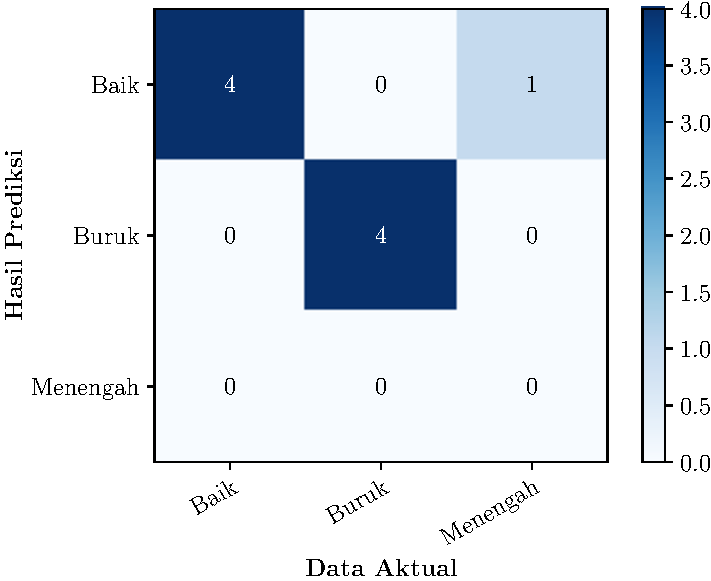
\includegraphics[width=0.6\textwidth]{BAB-4/plot/CM_1_layer_data_kecil.pdf}
		\captionof{figure}{Studi Kasus 2: \textit{Confusion Matrix} LSTM dengan 1 \textit{Hidden Layer}}
		\label{gambar:CM 1 layer DS-2}
	\end{minipage}
}

\centerline{\begin{minipage}{\linewidth}
		\centering
		\vspace{12 pt}
		%% Creator: Matplotlib, PGF backend
%%
%% To include the figure in your LaTeX document, write
%%   \input{<filename>.pgf}
%%
%% Make sure the required packages are loaded in your preamble
%%   \usepackage{pgf}
%%
%% Figures using additional raster images can only be included by \input if
%% they are in the same directory as the main LaTeX file. For loading figures
%% from other directories you can use the `import` package
%%   \usepackage{import}
%%
%% and then include the figures with
%%   \import{<path to file>}{<filename>.pgf}
%%
%% Matplotlib used the following preamble
%%
\begingroup%
\makeatletter%
\begin{pgfpicture}%
\pgfpathrectangle{\pgfpointorigin}{\pgfqpoint{5.640000in}{3.140000in}}%
\pgfusepath{use as bounding box, clip}%
\begin{pgfscope}%
\pgfsetbuttcap%
\pgfsetmiterjoin%
\pgfsetlinewidth{0.000000pt}%
\definecolor{currentstroke}{rgb}{1.000000,1.000000,1.000000}%
\pgfsetstrokecolor{currentstroke}%
\pgfsetstrokeopacity{0.000000}%
\pgfsetdash{}{0pt}%
\pgfpathmoveto{\pgfqpoint{0.000000in}{0.000000in}}%
\pgfpathlineto{\pgfqpoint{5.640000in}{0.000000in}}%
\pgfpathlineto{\pgfqpoint{5.640000in}{3.140000in}}%
\pgfpathlineto{\pgfqpoint{0.000000in}{3.140000in}}%
\pgfpathclose%
\pgfusepath{}%
\end{pgfscope}%
\begin{pgfscope}%
\pgfsetbuttcap%
\pgfsetmiterjoin%
\definecolor{currentfill}{rgb}{1.000000,1.000000,1.000000}%
\pgfsetfillcolor{currentfill}%
\pgfsetlinewidth{0.000000pt}%
\definecolor{currentstroke}{rgb}{0.000000,0.000000,0.000000}%
\pgfsetstrokecolor{currentstroke}%
\pgfsetstrokeopacity{0.000000}%
\pgfsetdash{}{0pt}%
\pgfpathmoveto{\pgfqpoint{0.453704in}{0.693723in}}%
\pgfpathlineto{\pgfqpoint{2.730000in}{0.693723in}}%
\pgfpathlineto{\pgfqpoint{2.730000in}{3.140000in}}%
\pgfpathlineto{\pgfqpoint{0.453704in}{3.140000in}}%
\pgfpathclose%
\pgfusepath{fill}%
\end{pgfscope}%
\begin{pgfscope}%
\pgfpathrectangle{\pgfqpoint{0.453704in}{0.693723in}}{\pgfqpoint{2.276296in}{2.446277in}}%
\pgfusepath{clip}%
\pgfsetbuttcap%
\pgfsetmiterjoin%
\definecolor{currentfill}{rgb}{0.121569,0.466667,0.705882}%
\pgfsetfillcolor{currentfill}%
\pgfsetlinewidth{0.000000pt}%
\definecolor{currentstroke}{rgb}{0.000000,0.000000,0.000000}%
\pgfsetstrokecolor{currentstroke}%
\pgfsetstrokeopacity{0.000000}%
\pgfsetdash{}{0pt}%
\pgfpathmoveto{\pgfqpoint{0.557172in}{0.693723in}}%
\pgfpathlineto{\pgfqpoint{0.902065in}{0.693723in}}%
\pgfpathlineto{\pgfqpoint{0.902065in}{2.472833in}}%
\pgfpathlineto{\pgfqpoint{0.557172in}{2.472833in}}%
\pgfpathclose%
\pgfusepath{fill}%
\end{pgfscope}%
\begin{pgfscope}%
\pgfpathrectangle{\pgfqpoint{0.453704in}{0.693723in}}{\pgfqpoint{2.276296in}{2.446277in}}%
\pgfusepath{clip}%
\pgfsetbuttcap%
\pgfsetmiterjoin%
\definecolor{currentfill}{rgb}{0.121569,0.466667,0.705882}%
\pgfsetfillcolor{currentfill}%
\pgfsetlinewidth{0.000000pt}%
\definecolor{currentstroke}{rgb}{0.000000,0.000000,0.000000}%
\pgfsetstrokecolor{currentstroke}%
\pgfsetstrokeopacity{0.000000}%
\pgfsetdash{}{0pt}%
\pgfpathmoveto{\pgfqpoint{1.419405in}{0.693723in}}%
\pgfpathlineto{\pgfqpoint{1.764299in}{0.693723in}}%
\pgfpathlineto{\pgfqpoint{1.764299in}{2.917611in}}%
\pgfpathlineto{\pgfqpoint{1.419405in}{2.917611in}}%
\pgfpathclose%
\pgfusepath{fill}%
\end{pgfscope}%
\begin{pgfscope}%
\pgfpathrectangle{\pgfqpoint{0.453704in}{0.693723in}}{\pgfqpoint{2.276296in}{2.446277in}}%
\pgfusepath{clip}%
\pgfsetbuttcap%
\pgfsetmiterjoin%
\definecolor{currentfill}{rgb}{0.121569,0.466667,0.705882}%
\pgfsetfillcolor{currentfill}%
\pgfsetlinewidth{0.000000pt}%
\definecolor{currentstroke}{rgb}{0.000000,0.000000,0.000000}%
\pgfsetstrokecolor{currentstroke}%
\pgfsetstrokeopacity{0.000000}%
\pgfsetdash{}{0pt}%
\pgfpathmoveto{\pgfqpoint{2.281639in}{0.693723in}}%
\pgfpathlineto{\pgfqpoint{2.626532in}{0.693723in}}%
\pgfpathlineto{\pgfqpoint{2.626532in}{0.693723in}}%
\pgfpathlineto{\pgfqpoint{2.281639in}{0.693723in}}%
\pgfpathclose%
\pgfusepath{fill}%
\end{pgfscope}%
\begin{pgfscope}%
\pgfsetbuttcap%
\pgfsetroundjoin%
\definecolor{currentfill}{rgb}{0.000000,0.000000,0.000000}%
\pgfsetfillcolor{currentfill}%
\pgfsetlinewidth{0.803000pt}%
\definecolor{currentstroke}{rgb}{0.000000,0.000000,0.000000}%
\pgfsetstrokecolor{currentstroke}%
\pgfsetdash{}{0pt}%
\pgfsys@defobject{currentmarker}{\pgfqpoint{0.000000in}{-0.048611in}}{\pgfqpoint{0.000000in}{0.000000in}}{%
\pgfpathmoveto{\pgfqpoint{0.000000in}{0.000000in}}%
\pgfpathlineto{\pgfqpoint{0.000000in}{-0.048611in}}%
\pgfusepath{stroke,fill}%
}%
\begin{pgfscope}%
\pgfsys@transformshift{0.729619in}{0.693723in}%
\pgfsys@useobject{currentmarker}{}%
\end{pgfscope}%
\end{pgfscope}%
\begin{pgfscope}%
\definecolor{textcolor}{rgb}{0.000000,0.000000,0.000000}%
\pgfsetstrokecolor{textcolor}%
\pgfsetfillcolor{textcolor}%
\pgftext[x=0.729619in,y=0.596500in,right,top,rotate=30.000000]{\color{textcolor}\rmfamily\fontsize{10.000000}{12.000000}\selectfont Baik}%
\end{pgfscope}%
\begin{pgfscope}%
\pgfsetbuttcap%
\pgfsetroundjoin%
\definecolor{currentfill}{rgb}{0.000000,0.000000,0.000000}%
\pgfsetfillcolor{currentfill}%
\pgfsetlinewidth{0.803000pt}%
\definecolor{currentstroke}{rgb}{0.000000,0.000000,0.000000}%
\pgfsetstrokecolor{currentstroke}%
\pgfsetdash{}{0pt}%
\pgfsys@defobject{currentmarker}{\pgfqpoint{0.000000in}{-0.048611in}}{\pgfqpoint{0.000000in}{0.000000in}}{%
\pgfpathmoveto{\pgfqpoint{0.000000in}{0.000000in}}%
\pgfpathlineto{\pgfqpoint{0.000000in}{-0.048611in}}%
\pgfusepath{stroke,fill}%
}%
\begin{pgfscope}%
\pgfsys@transformshift{1.591852in}{0.693723in}%
\pgfsys@useobject{currentmarker}{}%
\end{pgfscope}%
\end{pgfscope}%
\begin{pgfscope}%
\definecolor{textcolor}{rgb}{0.000000,0.000000,0.000000}%
\pgfsetstrokecolor{textcolor}%
\pgfsetfillcolor{textcolor}%
\pgftext[x=1.591852in,y=0.596500in,right,top,rotate=30.000000]{\color{textcolor}\rmfamily\fontsize{10.000000}{12.000000}\selectfont Buruk}%
\end{pgfscope}%
\begin{pgfscope}%
\pgfsetbuttcap%
\pgfsetroundjoin%
\definecolor{currentfill}{rgb}{0.000000,0.000000,0.000000}%
\pgfsetfillcolor{currentfill}%
\pgfsetlinewidth{0.803000pt}%
\definecolor{currentstroke}{rgb}{0.000000,0.000000,0.000000}%
\pgfsetstrokecolor{currentstroke}%
\pgfsetdash{}{0pt}%
\pgfsys@defobject{currentmarker}{\pgfqpoint{0.000000in}{-0.048611in}}{\pgfqpoint{0.000000in}{0.000000in}}{%
\pgfpathmoveto{\pgfqpoint{0.000000in}{0.000000in}}%
\pgfpathlineto{\pgfqpoint{0.000000in}{-0.048611in}}%
\pgfusepath{stroke,fill}%
}%
\begin{pgfscope}%
\pgfsys@transformshift{2.454085in}{0.693723in}%
\pgfsys@useobject{currentmarker}{}%
\end{pgfscope}%
\end{pgfscope}%
\begin{pgfscope}%
\definecolor{textcolor}{rgb}{0.000000,0.000000,0.000000}%
\pgfsetstrokecolor{textcolor}%
\pgfsetfillcolor{textcolor}%
\pgftext[x=2.454085in,y=0.596500in,right,top,rotate=30.000000]{\color{textcolor}\rmfamily\fontsize{10.000000}{12.000000}\selectfont Menengah}%
\end{pgfscope}%
\begin{pgfscope}%
\definecolor{textcolor}{rgb}{0.000000,0.000000,0.000000}%
\pgfsetstrokecolor{textcolor}%
\pgfsetfillcolor{textcolor}%
\pgftext[x=1.591852in,y=0.123457in,,top]{\color{textcolor}\rmfamily\fontsize{10.000000}{12.000000}\selectfont Kategori}%
\end{pgfscope}%
\begin{pgfscope}%
\pgfsetbuttcap%
\pgfsetroundjoin%
\definecolor{currentfill}{rgb}{0.000000,0.000000,0.000000}%
\pgfsetfillcolor{currentfill}%
\pgfsetlinewidth{0.803000pt}%
\definecolor{currentstroke}{rgb}{0.000000,0.000000,0.000000}%
\pgfsetstrokecolor{currentstroke}%
\pgfsetdash{}{0pt}%
\pgfsys@defobject{currentmarker}{\pgfqpoint{-0.048611in}{0.000000in}}{\pgfqpoint{-0.000000in}{0.000000in}}{%
\pgfpathmoveto{\pgfqpoint{-0.000000in}{0.000000in}}%
\pgfpathlineto{\pgfqpoint{-0.048611in}{0.000000in}}%
\pgfusepath{stroke,fill}%
}%
\begin{pgfscope}%
\pgfsys@transformshift{0.453704in}{0.693723in}%
\pgfsys@useobject{currentmarker}{}%
\end{pgfscope}%
\end{pgfscope}%
\begin{pgfscope}%
\definecolor{textcolor}{rgb}{0.000000,0.000000,0.000000}%
\pgfsetstrokecolor{textcolor}%
\pgfsetfillcolor{textcolor}%
\pgftext[x=0.179012in, y=0.645497in, left, base]{\color{textcolor}\rmfamily\fontsize{10.000000}{12.000000}\selectfont \(\displaystyle {0.0}\)}%
\end{pgfscope}%
\begin{pgfscope}%
\pgfsetbuttcap%
\pgfsetroundjoin%
\definecolor{currentfill}{rgb}{0.000000,0.000000,0.000000}%
\pgfsetfillcolor{currentfill}%
\pgfsetlinewidth{0.803000pt}%
\definecolor{currentstroke}{rgb}{0.000000,0.000000,0.000000}%
\pgfsetstrokecolor{currentstroke}%
\pgfsetdash{}{0pt}%
\pgfsys@defobject{currentmarker}{\pgfqpoint{-0.048611in}{0.000000in}}{\pgfqpoint{-0.000000in}{0.000000in}}{%
\pgfpathmoveto{\pgfqpoint{-0.000000in}{0.000000in}}%
\pgfpathlineto{\pgfqpoint{-0.048611in}{0.000000in}}%
\pgfusepath{stroke,fill}%
}%
\begin{pgfscope}%
\pgfsys@transformshift{0.453704in}{1.138500in}%
\pgfsys@useobject{currentmarker}{}%
\end{pgfscope}%
\end{pgfscope}%
\begin{pgfscope}%
\definecolor{textcolor}{rgb}{0.000000,0.000000,0.000000}%
\pgfsetstrokecolor{textcolor}%
\pgfsetfillcolor{textcolor}%
\pgftext[x=0.179012in, y=1.090275in, left, base]{\color{textcolor}\rmfamily\fontsize{10.000000}{12.000000}\selectfont \(\displaystyle {0.2}\)}%
\end{pgfscope}%
\begin{pgfscope}%
\pgfsetbuttcap%
\pgfsetroundjoin%
\definecolor{currentfill}{rgb}{0.000000,0.000000,0.000000}%
\pgfsetfillcolor{currentfill}%
\pgfsetlinewidth{0.803000pt}%
\definecolor{currentstroke}{rgb}{0.000000,0.000000,0.000000}%
\pgfsetstrokecolor{currentstroke}%
\pgfsetdash{}{0pt}%
\pgfsys@defobject{currentmarker}{\pgfqpoint{-0.048611in}{0.000000in}}{\pgfqpoint{-0.000000in}{0.000000in}}{%
\pgfpathmoveto{\pgfqpoint{-0.000000in}{0.000000in}}%
\pgfpathlineto{\pgfqpoint{-0.048611in}{0.000000in}}%
\pgfusepath{stroke,fill}%
}%
\begin{pgfscope}%
\pgfsys@transformshift{0.453704in}{1.583278in}%
\pgfsys@useobject{currentmarker}{}%
\end{pgfscope}%
\end{pgfscope}%
\begin{pgfscope}%
\definecolor{textcolor}{rgb}{0.000000,0.000000,0.000000}%
\pgfsetstrokecolor{textcolor}%
\pgfsetfillcolor{textcolor}%
\pgftext[x=0.179012in, y=1.535053in, left, base]{\color{textcolor}\rmfamily\fontsize{10.000000}{12.000000}\selectfont \(\displaystyle {0.4}\)}%
\end{pgfscope}%
\begin{pgfscope}%
\pgfsetbuttcap%
\pgfsetroundjoin%
\definecolor{currentfill}{rgb}{0.000000,0.000000,0.000000}%
\pgfsetfillcolor{currentfill}%
\pgfsetlinewidth{0.803000pt}%
\definecolor{currentstroke}{rgb}{0.000000,0.000000,0.000000}%
\pgfsetstrokecolor{currentstroke}%
\pgfsetdash{}{0pt}%
\pgfsys@defobject{currentmarker}{\pgfqpoint{-0.048611in}{0.000000in}}{\pgfqpoint{-0.000000in}{0.000000in}}{%
\pgfpathmoveto{\pgfqpoint{-0.000000in}{0.000000in}}%
\pgfpathlineto{\pgfqpoint{-0.048611in}{0.000000in}}%
\pgfusepath{stroke,fill}%
}%
\begin{pgfscope}%
\pgfsys@transformshift{0.453704in}{2.028056in}%
\pgfsys@useobject{currentmarker}{}%
\end{pgfscope}%
\end{pgfscope}%
\begin{pgfscope}%
\definecolor{textcolor}{rgb}{0.000000,0.000000,0.000000}%
\pgfsetstrokecolor{textcolor}%
\pgfsetfillcolor{textcolor}%
\pgftext[x=0.179012in, y=1.979831in, left, base]{\color{textcolor}\rmfamily\fontsize{10.000000}{12.000000}\selectfont \(\displaystyle {0.6}\)}%
\end{pgfscope}%
\begin{pgfscope}%
\pgfsetbuttcap%
\pgfsetroundjoin%
\definecolor{currentfill}{rgb}{0.000000,0.000000,0.000000}%
\pgfsetfillcolor{currentfill}%
\pgfsetlinewidth{0.803000pt}%
\definecolor{currentstroke}{rgb}{0.000000,0.000000,0.000000}%
\pgfsetstrokecolor{currentstroke}%
\pgfsetdash{}{0pt}%
\pgfsys@defobject{currentmarker}{\pgfqpoint{-0.048611in}{0.000000in}}{\pgfqpoint{-0.000000in}{0.000000in}}{%
\pgfpathmoveto{\pgfqpoint{-0.000000in}{0.000000in}}%
\pgfpathlineto{\pgfqpoint{-0.048611in}{0.000000in}}%
\pgfusepath{stroke,fill}%
}%
\begin{pgfscope}%
\pgfsys@transformshift{0.453704in}{2.472833in}%
\pgfsys@useobject{currentmarker}{}%
\end{pgfscope}%
\end{pgfscope}%
\begin{pgfscope}%
\definecolor{textcolor}{rgb}{0.000000,0.000000,0.000000}%
\pgfsetstrokecolor{textcolor}%
\pgfsetfillcolor{textcolor}%
\pgftext[x=0.179012in, y=2.424608in, left, base]{\color{textcolor}\rmfamily\fontsize{10.000000}{12.000000}\selectfont \(\displaystyle {0.8}\)}%
\end{pgfscope}%
\begin{pgfscope}%
\pgfsetbuttcap%
\pgfsetroundjoin%
\definecolor{currentfill}{rgb}{0.000000,0.000000,0.000000}%
\pgfsetfillcolor{currentfill}%
\pgfsetlinewidth{0.803000pt}%
\definecolor{currentstroke}{rgb}{0.000000,0.000000,0.000000}%
\pgfsetstrokecolor{currentstroke}%
\pgfsetdash{}{0pt}%
\pgfsys@defobject{currentmarker}{\pgfqpoint{-0.048611in}{0.000000in}}{\pgfqpoint{-0.000000in}{0.000000in}}{%
\pgfpathmoveto{\pgfqpoint{-0.000000in}{0.000000in}}%
\pgfpathlineto{\pgfqpoint{-0.048611in}{0.000000in}}%
\pgfusepath{stroke,fill}%
}%
\begin{pgfscope}%
\pgfsys@transformshift{0.453704in}{2.917611in}%
\pgfsys@useobject{currentmarker}{}%
\end{pgfscope}%
\end{pgfscope}%
\begin{pgfscope}%
\definecolor{textcolor}{rgb}{0.000000,0.000000,0.000000}%
\pgfsetstrokecolor{textcolor}%
\pgfsetfillcolor{textcolor}%
\pgftext[x=0.179012in, y=2.869386in, left, base]{\color{textcolor}\rmfamily\fontsize{10.000000}{12.000000}\selectfont \(\displaystyle {1.0}\)}%
\end{pgfscope}%
\begin{pgfscope}%
\definecolor{textcolor}{rgb}{0.000000,0.000000,0.000000}%
\pgfsetstrokecolor{textcolor}%
\pgfsetfillcolor{textcolor}%
\pgftext[x=0.123457in,y=1.916861in,,bottom,rotate=90.000000]{\color{textcolor}\rmfamily\fontsize{10.000000}{12.000000}\selectfont Presisi}%
\end{pgfscope}%
\begin{pgfscope}%
\pgfsetrectcap%
\pgfsetmiterjoin%
\pgfsetlinewidth{0.803000pt}%
\definecolor{currentstroke}{rgb}{0.000000,0.000000,0.000000}%
\pgfsetstrokecolor{currentstroke}%
\pgfsetdash{}{0pt}%
\pgfpathmoveto{\pgfqpoint{0.453704in}{0.693723in}}%
\pgfpathlineto{\pgfqpoint{0.453704in}{3.140000in}}%
\pgfusepath{stroke}%
\end{pgfscope}%
\begin{pgfscope}%
\pgfsetrectcap%
\pgfsetmiterjoin%
\pgfsetlinewidth{0.803000pt}%
\definecolor{currentstroke}{rgb}{0.000000,0.000000,0.000000}%
\pgfsetstrokecolor{currentstroke}%
\pgfsetdash{}{0pt}%
\pgfpathmoveto{\pgfqpoint{2.730000in}{0.693723in}}%
\pgfpathlineto{\pgfqpoint{2.730000in}{3.140000in}}%
\pgfusepath{stroke}%
\end{pgfscope}%
\begin{pgfscope}%
\pgfsetrectcap%
\pgfsetmiterjoin%
\pgfsetlinewidth{0.803000pt}%
\definecolor{currentstroke}{rgb}{0.000000,0.000000,0.000000}%
\pgfsetstrokecolor{currentstroke}%
\pgfsetdash{}{0pt}%
\pgfpathmoveto{\pgfqpoint{0.453704in}{0.693723in}}%
\pgfpathlineto{\pgfqpoint{2.730000in}{0.693723in}}%
\pgfusepath{stroke}%
\end{pgfscope}%
\begin{pgfscope}%
\pgfsetrectcap%
\pgfsetmiterjoin%
\pgfsetlinewidth{0.803000pt}%
\definecolor{currentstroke}{rgb}{0.000000,0.000000,0.000000}%
\pgfsetstrokecolor{currentstroke}%
\pgfsetdash{}{0pt}%
\pgfpathmoveto{\pgfqpoint{0.453704in}{3.140000in}}%
\pgfpathlineto{\pgfqpoint{2.730000in}{3.140000in}}%
\pgfusepath{stroke}%
\end{pgfscope}%
\begin{pgfscope}%
\definecolor{textcolor}{rgb}{0.000000,0.000000,0.000000}%
\pgfsetstrokecolor{textcolor}%
\pgfsetfillcolor{textcolor}%
\pgftext[x=0.729619in,y=2.495072in,,bottom]{\color{textcolor}\rmfamily\fontsize{9.000000}{10.800000}\selectfont 0.8}%
\end{pgfscope}%
\begin{pgfscope}%
\definecolor{textcolor}{rgb}{0.000000,0.000000,0.000000}%
\pgfsetstrokecolor{textcolor}%
\pgfsetfillcolor{textcolor}%
\pgftext[x=1.591852in,y=2.939850in,,bottom]{\color{textcolor}\rmfamily\fontsize{9.000000}{10.800000}\selectfont 1.0}%
\end{pgfscope}%
\begin{pgfscope}%
\definecolor{textcolor}{rgb}{0.000000,0.000000,0.000000}%
\pgfsetstrokecolor{textcolor}%
\pgfsetfillcolor{textcolor}%
\pgftext[x=2.454085in,y=0.715962in,,bottom]{\color{textcolor}\rmfamily\fontsize{9.000000}{10.800000}\selectfont 0.0}%
\end{pgfscope}%
\begin{pgfscope}%
\pgfsetbuttcap%
\pgfsetmiterjoin%
\definecolor{currentfill}{rgb}{1.000000,1.000000,1.000000}%
\pgfsetfillcolor{currentfill}%
\pgfsetlinewidth{0.000000pt}%
\definecolor{currentstroke}{rgb}{0.000000,0.000000,0.000000}%
\pgfsetstrokecolor{currentstroke}%
\pgfsetstrokeopacity{0.000000}%
\pgfsetdash{}{0pt}%
\pgfpathmoveto{\pgfqpoint{3.363704in}{0.693723in}}%
\pgfpathlineto{\pgfqpoint{5.640000in}{0.693723in}}%
\pgfpathlineto{\pgfqpoint{5.640000in}{3.140000in}}%
\pgfpathlineto{\pgfqpoint{3.363704in}{3.140000in}}%
\pgfpathclose%
\pgfusepath{fill}%
\end{pgfscope}%
\begin{pgfscope}%
\pgfpathrectangle{\pgfqpoint{3.363704in}{0.693723in}}{\pgfqpoint{2.276296in}{2.446277in}}%
\pgfusepath{clip}%
\pgfsetbuttcap%
\pgfsetmiterjoin%
\definecolor{currentfill}{rgb}{1.000000,0.498039,0.054902}%
\pgfsetfillcolor{currentfill}%
\pgfsetlinewidth{0.000000pt}%
\definecolor{currentstroke}{rgb}{0.000000,0.000000,0.000000}%
\pgfsetstrokecolor{currentstroke}%
\pgfsetstrokeopacity{0.000000}%
\pgfsetdash{}{0pt}%
\pgfpathmoveto{\pgfqpoint{3.467172in}{0.693723in}}%
\pgfpathlineto{\pgfqpoint{3.812065in}{0.693723in}}%
\pgfpathlineto{\pgfqpoint{3.812065in}{2.917611in}}%
\pgfpathlineto{\pgfqpoint{3.467172in}{2.917611in}}%
\pgfpathclose%
\pgfusepath{fill}%
\end{pgfscope}%
\begin{pgfscope}%
\pgfpathrectangle{\pgfqpoint{3.363704in}{0.693723in}}{\pgfqpoint{2.276296in}{2.446277in}}%
\pgfusepath{clip}%
\pgfsetbuttcap%
\pgfsetmiterjoin%
\definecolor{currentfill}{rgb}{1.000000,0.498039,0.054902}%
\pgfsetfillcolor{currentfill}%
\pgfsetlinewidth{0.000000pt}%
\definecolor{currentstroke}{rgb}{0.000000,0.000000,0.000000}%
\pgfsetstrokecolor{currentstroke}%
\pgfsetstrokeopacity{0.000000}%
\pgfsetdash{}{0pt}%
\pgfpathmoveto{\pgfqpoint{4.329405in}{0.693723in}}%
\pgfpathlineto{\pgfqpoint{4.674299in}{0.693723in}}%
\pgfpathlineto{\pgfqpoint{4.674299in}{2.917611in}}%
\pgfpathlineto{\pgfqpoint{4.329405in}{2.917611in}}%
\pgfpathclose%
\pgfusepath{fill}%
\end{pgfscope}%
\begin{pgfscope}%
\pgfpathrectangle{\pgfqpoint{3.363704in}{0.693723in}}{\pgfqpoint{2.276296in}{2.446277in}}%
\pgfusepath{clip}%
\pgfsetbuttcap%
\pgfsetmiterjoin%
\definecolor{currentfill}{rgb}{1.000000,0.498039,0.054902}%
\pgfsetfillcolor{currentfill}%
\pgfsetlinewidth{0.000000pt}%
\definecolor{currentstroke}{rgb}{0.000000,0.000000,0.000000}%
\pgfsetstrokecolor{currentstroke}%
\pgfsetstrokeopacity{0.000000}%
\pgfsetdash{}{0pt}%
\pgfpathmoveto{\pgfqpoint{5.191639in}{0.693723in}}%
\pgfpathlineto{\pgfqpoint{5.536532in}{0.693723in}}%
\pgfpathlineto{\pgfqpoint{5.536532in}{0.693723in}}%
\pgfpathlineto{\pgfqpoint{5.191639in}{0.693723in}}%
\pgfpathclose%
\pgfusepath{fill}%
\end{pgfscope}%
\begin{pgfscope}%
\pgfsetbuttcap%
\pgfsetroundjoin%
\definecolor{currentfill}{rgb}{0.000000,0.000000,0.000000}%
\pgfsetfillcolor{currentfill}%
\pgfsetlinewidth{0.803000pt}%
\definecolor{currentstroke}{rgb}{0.000000,0.000000,0.000000}%
\pgfsetstrokecolor{currentstroke}%
\pgfsetdash{}{0pt}%
\pgfsys@defobject{currentmarker}{\pgfqpoint{0.000000in}{-0.048611in}}{\pgfqpoint{0.000000in}{0.000000in}}{%
\pgfpathmoveto{\pgfqpoint{0.000000in}{0.000000in}}%
\pgfpathlineto{\pgfqpoint{0.000000in}{-0.048611in}}%
\pgfusepath{stroke,fill}%
}%
\begin{pgfscope}%
\pgfsys@transformshift{3.639619in}{0.693723in}%
\pgfsys@useobject{currentmarker}{}%
\end{pgfscope}%
\end{pgfscope}%
\begin{pgfscope}%
\definecolor{textcolor}{rgb}{0.000000,0.000000,0.000000}%
\pgfsetstrokecolor{textcolor}%
\pgfsetfillcolor{textcolor}%
\pgftext[x=3.639619in,y=0.596500in,right,top,rotate=30.000000]{\color{textcolor}\rmfamily\fontsize{10.000000}{12.000000}\selectfont Baik}%
\end{pgfscope}%
\begin{pgfscope}%
\pgfsetbuttcap%
\pgfsetroundjoin%
\definecolor{currentfill}{rgb}{0.000000,0.000000,0.000000}%
\pgfsetfillcolor{currentfill}%
\pgfsetlinewidth{0.803000pt}%
\definecolor{currentstroke}{rgb}{0.000000,0.000000,0.000000}%
\pgfsetstrokecolor{currentstroke}%
\pgfsetdash{}{0pt}%
\pgfsys@defobject{currentmarker}{\pgfqpoint{0.000000in}{-0.048611in}}{\pgfqpoint{0.000000in}{0.000000in}}{%
\pgfpathmoveto{\pgfqpoint{0.000000in}{0.000000in}}%
\pgfpathlineto{\pgfqpoint{0.000000in}{-0.048611in}}%
\pgfusepath{stroke,fill}%
}%
\begin{pgfscope}%
\pgfsys@transformshift{4.501852in}{0.693723in}%
\pgfsys@useobject{currentmarker}{}%
\end{pgfscope}%
\end{pgfscope}%
\begin{pgfscope}%
\definecolor{textcolor}{rgb}{0.000000,0.000000,0.000000}%
\pgfsetstrokecolor{textcolor}%
\pgfsetfillcolor{textcolor}%
\pgftext[x=4.501852in,y=0.596500in,right,top,rotate=30.000000]{\color{textcolor}\rmfamily\fontsize{10.000000}{12.000000}\selectfont Buruk}%
\end{pgfscope}%
\begin{pgfscope}%
\pgfsetbuttcap%
\pgfsetroundjoin%
\definecolor{currentfill}{rgb}{0.000000,0.000000,0.000000}%
\pgfsetfillcolor{currentfill}%
\pgfsetlinewidth{0.803000pt}%
\definecolor{currentstroke}{rgb}{0.000000,0.000000,0.000000}%
\pgfsetstrokecolor{currentstroke}%
\pgfsetdash{}{0pt}%
\pgfsys@defobject{currentmarker}{\pgfqpoint{0.000000in}{-0.048611in}}{\pgfqpoint{0.000000in}{0.000000in}}{%
\pgfpathmoveto{\pgfqpoint{0.000000in}{0.000000in}}%
\pgfpathlineto{\pgfqpoint{0.000000in}{-0.048611in}}%
\pgfusepath{stroke,fill}%
}%
\begin{pgfscope}%
\pgfsys@transformshift{5.364085in}{0.693723in}%
\pgfsys@useobject{currentmarker}{}%
\end{pgfscope}%
\end{pgfscope}%
\begin{pgfscope}%
\definecolor{textcolor}{rgb}{0.000000,0.000000,0.000000}%
\pgfsetstrokecolor{textcolor}%
\pgfsetfillcolor{textcolor}%
\pgftext[x=5.364085in,y=0.596500in,right,top,rotate=30.000000]{\color{textcolor}\rmfamily\fontsize{10.000000}{12.000000}\selectfont Menengah}%
\end{pgfscope}%
\begin{pgfscope}%
\definecolor{textcolor}{rgb}{0.000000,0.000000,0.000000}%
\pgfsetstrokecolor{textcolor}%
\pgfsetfillcolor{textcolor}%
\pgftext[x=4.501852in,y=0.123457in,,top]{\color{textcolor}\rmfamily\fontsize{10.000000}{12.000000}\selectfont Kategori}%
\end{pgfscope}%
\begin{pgfscope}%
\pgfsetbuttcap%
\pgfsetroundjoin%
\definecolor{currentfill}{rgb}{0.000000,0.000000,0.000000}%
\pgfsetfillcolor{currentfill}%
\pgfsetlinewidth{0.803000pt}%
\definecolor{currentstroke}{rgb}{0.000000,0.000000,0.000000}%
\pgfsetstrokecolor{currentstroke}%
\pgfsetdash{}{0pt}%
\pgfsys@defobject{currentmarker}{\pgfqpoint{-0.048611in}{0.000000in}}{\pgfqpoint{-0.000000in}{0.000000in}}{%
\pgfpathmoveto{\pgfqpoint{-0.000000in}{0.000000in}}%
\pgfpathlineto{\pgfqpoint{-0.048611in}{0.000000in}}%
\pgfusepath{stroke,fill}%
}%
\begin{pgfscope}%
\pgfsys@transformshift{3.363704in}{0.693723in}%
\pgfsys@useobject{currentmarker}{}%
\end{pgfscope}%
\end{pgfscope}%
\begin{pgfscope}%
\definecolor{textcolor}{rgb}{0.000000,0.000000,0.000000}%
\pgfsetstrokecolor{textcolor}%
\pgfsetfillcolor{textcolor}%
\pgftext[x=3.089012in, y=0.645497in, left, base]{\color{textcolor}\rmfamily\fontsize{10.000000}{12.000000}\selectfont \(\displaystyle {0.0}\)}%
\end{pgfscope}%
\begin{pgfscope}%
\pgfsetbuttcap%
\pgfsetroundjoin%
\definecolor{currentfill}{rgb}{0.000000,0.000000,0.000000}%
\pgfsetfillcolor{currentfill}%
\pgfsetlinewidth{0.803000pt}%
\definecolor{currentstroke}{rgb}{0.000000,0.000000,0.000000}%
\pgfsetstrokecolor{currentstroke}%
\pgfsetdash{}{0pt}%
\pgfsys@defobject{currentmarker}{\pgfqpoint{-0.048611in}{0.000000in}}{\pgfqpoint{-0.000000in}{0.000000in}}{%
\pgfpathmoveto{\pgfqpoint{-0.000000in}{0.000000in}}%
\pgfpathlineto{\pgfqpoint{-0.048611in}{0.000000in}}%
\pgfusepath{stroke,fill}%
}%
\begin{pgfscope}%
\pgfsys@transformshift{3.363704in}{1.138500in}%
\pgfsys@useobject{currentmarker}{}%
\end{pgfscope}%
\end{pgfscope}%
\begin{pgfscope}%
\definecolor{textcolor}{rgb}{0.000000,0.000000,0.000000}%
\pgfsetstrokecolor{textcolor}%
\pgfsetfillcolor{textcolor}%
\pgftext[x=3.089012in, y=1.090275in, left, base]{\color{textcolor}\rmfamily\fontsize{10.000000}{12.000000}\selectfont \(\displaystyle {0.2}\)}%
\end{pgfscope}%
\begin{pgfscope}%
\pgfsetbuttcap%
\pgfsetroundjoin%
\definecolor{currentfill}{rgb}{0.000000,0.000000,0.000000}%
\pgfsetfillcolor{currentfill}%
\pgfsetlinewidth{0.803000pt}%
\definecolor{currentstroke}{rgb}{0.000000,0.000000,0.000000}%
\pgfsetstrokecolor{currentstroke}%
\pgfsetdash{}{0pt}%
\pgfsys@defobject{currentmarker}{\pgfqpoint{-0.048611in}{0.000000in}}{\pgfqpoint{-0.000000in}{0.000000in}}{%
\pgfpathmoveto{\pgfqpoint{-0.000000in}{0.000000in}}%
\pgfpathlineto{\pgfqpoint{-0.048611in}{0.000000in}}%
\pgfusepath{stroke,fill}%
}%
\begin{pgfscope}%
\pgfsys@transformshift{3.363704in}{1.583278in}%
\pgfsys@useobject{currentmarker}{}%
\end{pgfscope}%
\end{pgfscope}%
\begin{pgfscope}%
\definecolor{textcolor}{rgb}{0.000000,0.000000,0.000000}%
\pgfsetstrokecolor{textcolor}%
\pgfsetfillcolor{textcolor}%
\pgftext[x=3.089012in, y=1.535053in, left, base]{\color{textcolor}\rmfamily\fontsize{10.000000}{12.000000}\selectfont \(\displaystyle {0.4}\)}%
\end{pgfscope}%
\begin{pgfscope}%
\pgfsetbuttcap%
\pgfsetroundjoin%
\definecolor{currentfill}{rgb}{0.000000,0.000000,0.000000}%
\pgfsetfillcolor{currentfill}%
\pgfsetlinewidth{0.803000pt}%
\definecolor{currentstroke}{rgb}{0.000000,0.000000,0.000000}%
\pgfsetstrokecolor{currentstroke}%
\pgfsetdash{}{0pt}%
\pgfsys@defobject{currentmarker}{\pgfqpoint{-0.048611in}{0.000000in}}{\pgfqpoint{-0.000000in}{0.000000in}}{%
\pgfpathmoveto{\pgfqpoint{-0.000000in}{0.000000in}}%
\pgfpathlineto{\pgfqpoint{-0.048611in}{0.000000in}}%
\pgfusepath{stroke,fill}%
}%
\begin{pgfscope}%
\pgfsys@transformshift{3.363704in}{2.028056in}%
\pgfsys@useobject{currentmarker}{}%
\end{pgfscope}%
\end{pgfscope}%
\begin{pgfscope}%
\definecolor{textcolor}{rgb}{0.000000,0.000000,0.000000}%
\pgfsetstrokecolor{textcolor}%
\pgfsetfillcolor{textcolor}%
\pgftext[x=3.089012in, y=1.979831in, left, base]{\color{textcolor}\rmfamily\fontsize{10.000000}{12.000000}\selectfont \(\displaystyle {0.6}\)}%
\end{pgfscope}%
\begin{pgfscope}%
\pgfsetbuttcap%
\pgfsetroundjoin%
\definecolor{currentfill}{rgb}{0.000000,0.000000,0.000000}%
\pgfsetfillcolor{currentfill}%
\pgfsetlinewidth{0.803000pt}%
\definecolor{currentstroke}{rgb}{0.000000,0.000000,0.000000}%
\pgfsetstrokecolor{currentstroke}%
\pgfsetdash{}{0pt}%
\pgfsys@defobject{currentmarker}{\pgfqpoint{-0.048611in}{0.000000in}}{\pgfqpoint{-0.000000in}{0.000000in}}{%
\pgfpathmoveto{\pgfqpoint{-0.000000in}{0.000000in}}%
\pgfpathlineto{\pgfqpoint{-0.048611in}{0.000000in}}%
\pgfusepath{stroke,fill}%
}%
\begin{pgfscope}%
\pgfsys@transformshift{3.363704in}{2.472833in}%
\pgfsys@useobject{currentmarker}{}%
\end{pgfscope}%
\end{pgfscope}%
\begin{pgfscope}%
\definecolor{textcolor}{rgb}{0.000000,0.000000,0.000000}%
\pgfsetstrokecolor{textcolor}%
\pgfsetfillcolor{textcolor}%
\pgftext[x=3.089012in, y=2.424608in, left, base]{\color{textcolor}\rmfamily\fontsize{10.000000}{12.000000}\selectfont \(\displaystyle {0.8}\)}%
\end{pgfscope}%
\begin{pgfscope}%
\pgfsetbuttcap%
\pgfsetroundjoin%
\definecolor{currentfill}{rgb}{0.000000,0.000000,0.000000}%
\pgfsetfillcolor{currentfill}%
\pgfsetlinewidth{0.803000pt}%
\definecolor{currentstroke}{rgb}{0.000000,0.000000,0.000000}%
\pgfsetstrokecolor{currentstroke}%
\pgfsetdash{}{0pt}%
\pgfsys@defobject{currentmarker}{\pgfqpoint{-0.048611in}{0.000000in}}{\pgfqpoint{-0.000000in}{0.000000in}}{%
\pgfpathmoveto{\pgfqpoint{-0.000000in}{0.000000in}}%
\pgfpathlineto{\pgfqpoint{-0.048611in}{0.000000in}}%
\pgfusepath{stroke,fill}%
}%
\begin{pgfscope}%
\pgfsys@transformshift{3.363704in}{2.917611in}%
\pgfsys@useobject{currentmarker}{}%
\end{pgfscope}%
\end{pgfscope}%
\begin{pgfscope}%
\definecolor{textcolor}{rgb}{0.000000,0.000000,0.000000}%
\pgfsetstrokecolor{textcolor}%
\pgfsetfillcolor{textcolor}%
\pgftext[x=3.089012in, y=2.869386in, left, base]{\color{textcolor}\rmfamily\fontsize{10.000000}{12.000000}\selectfont \(\displaystyle {1.0}\)}%
\end{pgfscope}%
\begin{pgfscope}%
\definecolor{textcolor}{rgb}{0.000000,0.000000,0.000000}%
\pgfsetstrokecolor{textcolor}%
\pgfsetfillcolor{textcolor}%
\pgftext[x=3.033457in,y=1.916861in,,bottom,rotate=90.000000]{\color{textcolor}\rmfamily\fontsize{10.000000}{12.000000}\selectfont Sensitivity}%
\end{pgfscope}%
\begin{pgfscope}%
\pgfsetrectcap%
\pgfsetmiterjoin%
\pgfsetlinewidth{0.803000pt}%
\definecolor{currentstroke}{rgb}{0.000000,0.000000,0.000000}%
\pgfsetstrokecolor{currentstroke}%
\pgfsetdash{}{0pt}%
\pgfpathmoveto{\pgfqpoint{3.363704in}{0.693723in}}%
\pgfpathlineto{\pgfqpoint{3.363704in}{3.140000in}}%
\pgfusepath{stroke}%
\end{pgfscope}%
\begin{pgfscope}%
\pgfsetrectcap%
\pgfsetmiterjoin%
\pgfsetlinewidth{0.803000pt}%
\definecolor{currentstroke}{rgb}{0.000000,0.000000,0.000000}%
\pgfsetstrokecolor{currentstroke}%
\pgfsetdash{}{0pt}%
\pgfpathmoveto{\pgfqpoint{5.640000in}{0.693723in}}%
\pgfpathlineto{\pgfqpoint{5.640000in}{3.140000in}}%
\pgfusepath{stroke}%
\end{pgfscope}%
\begin{pgfscope}%
\pgfsetrectcap%
\pgfsetmiterjoin%
\pgfsetlinewidth{0.803000pt}%
\definecolor{currentstroke}{rgb}{0.000000,0.000000,0.000000}%
\pgfsetstrokecolor{currentstroke}%
\pgfsetdash{}{0pt}%
\pgfpathmoveto{\pgfqpoint{3.363704in}{0.693723in}}%
\pgfpathlineto{\pgfqpoint{5.640000in}{0.693723in}}%
\pgfusepath{stroke}%
\end{pgfscope}%
\begin{pgfscope}%
\pgfsetrectcap%
\pgfsetmiterjoin%
\pgfsetlinewidth{0.803000pt}%
\definecolor{currentstroke}{rgb}{0.000000,0.000000,0.000000}%
\pgfsetstrokecolor{currentstroke}%
\pgfsetdash{}{0pt}%
\pgfpathmoveto{\pgfqpoint{3.363704in}{3.140000in}}%
\pgfpathlineto{\pgfqpoint{5.640000in}{3.140000in}}%
\pgfusepath{stroke}%
\end{pgfscope}%
\begin{pgfscope}%
\definecolor{textcolor}{rgb}{0.000000,0.000000,0.000000}%
\pgfsetstrokecolor{textcolor}%
\pgfsetfillcolor{textcolor}%
\pgftext[x=3.639619in,y=2.939850in,,bottom]{\color{textcolor}\rmfamily\fontsize{9.000000}{10.800000}\selectfont 1.0}%
\end{pgfscope}%
\begin{pgfscope}%
\definecolor{textcolor}{rgb}{0.000000,0.000000,0.000000}%
\pgfsetstrokecolor{textcolor}%
\pgfsetfillcolor{textcolor}%
\pgftext[x=4.501852in,y=2.939850in,,bottom]{\color{textcolor}\rmfamily\fontsize{9.000000}{10.800000}\selectfont 1.0}%
\end{pgfscope}%
\begin{pgfscope}%
\definecolor{textcolor}{rgb}{0.000000,0.000000,0.000000}%
\pgfsetstrokecolor{textcolor}%
\pgfsetfillcolor{textcolor}%
\pgftext[x=5.364085in,y=0.715962in,,bottom]{\color{textcolor}\rmfamily\fontsize{9.000000}{10.800000}\selectfont 0.0}%
\end{pgfscope}%
\end{pgfpicture}%
\makeatother%
\endgroup%

		\captionof{figure}{Studi Kasus 2: Presisi Percobaan Perubahan Layer}
		\label{gambar:presisi sensitivity 1 layer data kecil}
\end{minipage}}

Perolehan hasil percobaan yang disajikan pada Gambar \ref{gambar:CM 1 layer DS-2} serta Gambar \ref{gambar:presisi sensitivity 1 layer data kecil} memperlihatkan bahwa model belum bisa melakukan diagnosis indeks kesehatan transformator daya pada kategori "Menengah". Hal ini ditandai dengan nilai presisi dan sensitivitas yang masil 0. Oleh karena itu masih perlu dilakukan percobaan lanjutan untuk memperbaiki akurasi model LSTM tersebut. Percobaan dilakukan seperti halnya pada studi kasus pertama yang melakukan perubahan  \textit{hyperparameter} pada penggunaan fungsi aktivasi yang berbeda. \par

\subsection{Perubahan Fungsi Aktivasi}
Jenis fungsi aktivasi yang digunakan pada percobaan ini adalah yang tersedia pada \textit{library} Keras yakni \textit{tanh, relu, softmax, selu, elu, softplus,} dan \textit{softsign}. Pada Gambar \ref{gambar:perbandingan fungsi aktivasi data kecil} merupakan representasi hasil percobaan tersebut.


\centerline{\begin{minipage}{\linewidth}
		\vspace{12 pt}
		\centering
		%% Creator: Matplotlib, PGF backend
%%
%% To include the figure in your LaTeX document, write
%%   \input{<filename>.pgf}
%%
%% Make sure the required packages are loaded in your preamble
%%   \usepackage{pgf}
%%
%% Figures using additional raster images can only be included by \input if
%% they are in the same directory as the main LaTeX file. For loading figures
%% from other directories you can use the `import` package
%%   \usepackage{import}
%%
%% and then include the figures with
%%   \import{<path to file>}{<filename>.pgf}
%%
%% Matplotlib used the following preamble
%%
\begingroup%
\makeatletter%
\begin{pgfpicture}%
\pgfpathrectangle{\pgfpointorigin}{\pgfqpoint{6.000000in}{4.000000in}}%
\pgfusepath{use as bounding box, clip}%
\begin{pgfscope}%
\pgfsetbuttcap%
\pgfsetmiterjoin%
\pgfsetlinewidth{0.000000pt}%
\definecolor{currentstroke}{rgb}{1.000000,1.000000,1.000000}%
\pgfsetstrokecolor{currentstroke}%
\pgfsetstrokeopacity{0.000000}%
\pgfsetdash{}{0pt}%
\pgfpathmoveto{\pgfqpoint{0.000000in}{0.000000in}}%
\pgfpathlineto{\pgfqpoint{6.000000in}{0.000000in}}%
\pgfpathlineto{\pgfqpoint{6.000000in}{4.000000in}}%
\pgfpathlineto{\pgfqpoint{0.000000in}{4.000000in}}%
\pgfpathclose%
\pgfusepath{}%
\end{pgfscope}%
\begin{pgfscope}%
\pgfsetbuttcap%
\pgfsetmiterjoin%
\definecolor{currentfill}{rgb}{1.000000,1.000000,1.000000}%
\pgfsetfillcolor{currentfill}%
\pgfsetlinewidth{0.000000pt}%
\definecolor{currentstroke}{rgb}{0.000000,0.000000,0.000000}%
\pgfsetstrokecolor{currentstroke}%
\pgfsetstrokeopacity{0.000000}%
\pgfsetdash{}{0pt}%
\pgfpathmoveto{\pgfqpoint{0.750000in}{0.500000in}}%
\pgfpathlineto{\pgfqpoint{5.400000in}{0.500000in}}%
\pgfpathlineto{\pgfqpoint{5.400000in}{3.520000in}}%
\pgfpathlineto{\pgfqpoint{0.750000in}{3.520000in}}%
\pgfpathclose%
\pgfusepath{fill}%
\end{pgfscope}%
\begin{pgfscope}%
\pgfpathrectangle{\pgfqpoint{0.750000in}{0.500000in}}{\pgfqpoint{4.650000in}{3.020000in}}%
\pgfusepath{clip}%
\pgfsetbuttcap%
\pgfsetmiterjoin%
\definecolor{currentfill}{rgb}{0.121569,0.466667,0.705882}%
\pgfsetfillcolor{currentfill}%
\pgfsetlinewidth{0.000000pt}%
\definecolor{currentstroke}{rgb}{0.000000,0.000000,0.000000}%
\pgfsetstrokecolor{currentstroke}%
\pgfsetstrokeopacity{0.000000}%
\pgfsetdash{}{0pt}%
\pgfpathmoveto{\pgfqpoint{0.961364in}{-3.124000in}}%
\pgfpathlineto{\pgfqpoint{1.128230in}{-3.124000in}}%
\pgfpathlineto{\pgfqpoint{1.128230in}{1.726120in}}%
\pgfpathlineto{\pgfqpoint{0.961364in}{1.726120in}}%
\pgfpathclose%
\pgfusepath{fill}%
\end{pgfscope}%
\begin{pgfscope}%
\pgfpathrectangle{\pgfqpoint{0.750000in}{0.500000in}}{\pgfqpoint{4.650000in}{3.020000in}}%
\pgfusepath{clip}%
\pgfsetbuttcap%
\pgfsetmiterjoin%
\definecolor{currentfill}{rgb}{0.121569,0.466667,0.705882}%
\pgfsetfillcolor{currentfill}%
\pgfsetlinewidth{0.000000pt}%
\definecolor{currentstroke}{rgb}{0.000000,0.000000,0.000000}%
\pgfsetstrokecolor{currentstroke}%
\pgfsetstrokeopacity{0.000000}%
\pgfsetdash{}{0pt}%
\pgfpathmoveto{\pgfqpoint{1.517584in}{-3.124000in}}%
\pgfpathlineto{\pgfqpoint{1.684450in}{-3.124000in}}%
\pgfpathlineto{\pgfqpoint{1.684450in}{1.871080in}}%
\pgfpathlineto{\pgfqpoint{1.517584in}{1.871080in}}%
\pgfpathclose%
\pgfusepath{fill}%
\end{pgfscope}%
\begin{pgfscope}%
\pgfpathrectangle{\pgfqpoint{0.750000in}{0.500000in}}{\pgfqpoint{4.650000in}{3.020000in}}%
\pgfusepath{clip}%
\pgfsetbuttcap%
\pgfsetmiterjoin%
\definecolor{currentfill}{rgb}{0.121569,0.466667,0.705882}%
\pgfsetfillcolor{currentfill}%
\pgfsetlinewidth{0.000000pt}%
\definecolor{currentstroke}{rgb}{0.000000,0.000000,0.000000}%
\pgfsetstrokecolor{currentstroke}%
\pgfsetstrokeopacity{0.000000}%
\pgfsetdash{}{0pt}%
\pgfpathmoveto{\pgfqpoint{2.073804in}{-3.124000in}}%
\pgfpathlineto{\pgfqpoint{2.240670in}{-3.124000in}}%
\pgfpathlineto{\pgfqpoint{2.240670in}{2.003960in}}%
\pgfpathlineto{\pgfqpoint{2.073804in}{2.003960in}}%
\pgfpathclose%
\pgfusepath{fill}%
\end{pgfscope}%
\begin{pgfscope}%
\pgfpathrectangle{\pgfqpoint{0.750000in}{0.500000in}}{\pgfqpoint{4.650000in}{3.020000in}}%
\pgfusepath{clip}%
\pgfsetbuttcap%
\pgfsetmiterjoin%
\definecolor{currentfill}{rgb}{0.121569,0.466667,0.705882}%
\pgfsetfillcolor{currentfill}%
\pgfsetlinewidth{0.000000pt}%
\definecolor{currentstroke}{rgb}{0.000000,0.000000,0.000000}%
\pgfsetstrokecolor{currentstroke}%
\pgfsetstrokeopacity{0.000000}%
\pgfsetdash{}{0pt}%
\pgfpathmoveto{\pgfqpoint{2.630024in}{-3.124000in}}%
\pgfpathlineto{\pgfqpoint{2.796890in}{-3.124000in}}%
\pgfpathlineto{\pgfqpoint{2.796890in}{1.315400in}}%
\pgfpathlineto{\pgfqpoint{2.630024in}{1.315400in}}%
\pgfpathclose%
\pgfusepath{fill}%
\end{pgfscope}%
\begin{pgfscope}%
\pgfpathrectangle{\pgfqpoint{0.750000in}{0.500000in}}{\pgfqpoint{4.650000in}{3.020000in}}%
\pgfusepath{clip}%
\pgfsetbuttcap%
\pgfsetmiterjoin%
\definecolor{currentfill}{rgb}{0.121569,0.466667,0.705882}%
\pgfsetfillcolor{currentfill}%
\pgfsetlinewidth{0.000000pt}%
\definecolor{currentstroke}{rgb}{0.000000,0.000000,0.000000}%
\pgfsetstrokecolor{currentstroke}%
\pgfsetstrokeopacity{0.000000}%
\pgfsetdash{}{0pt}%
\pgfpathmoveto{\pgfqpoint{3.186244in}{-3.124000in}}%
\pgfpathlineto{\pgfqpoint{3.353110in}{-3.124000in}}%
\pgfpathlineto{\pgfqpoint{3.353110in}{2.148920in}}%
\pgfpathlineto{\pgfqpoint{3.186244in}{2.148920in}}%
\pgfpathclose%
\pgfusepath{fill}%
\end{pgfscope}%
\begin{pgfscope}%
\pgfpathrectangle{\pgfqpoint{0.750000in}{0.500000in}}{\pgfqpoint{4.650000in}{3.020000in}}%
\pgfusepath{clip}%
\pgfsetbuttcap%
\pgfsetmiterjoin%
\definecolor{currentfill}{rgb}{0.121569,0.466667,0.705882}%
\pgfsetfillcolor{currentfill}%
\pgfsetlinewidth{0.000000pt}%
\definecolor{currentstroke}{rgb}{0.000000,0.000000,0.000000}%
\pgfsetstrokecolor{currentstroke}%
\pgfsetstrokeopacity{0.000000}%
\pgfsetdash{}{0pt}%
\pgfpathmoveto{\pgfqpoint{3.742464in}{-3.124000in}}%
\pgfpathlineto{\pgfqpoint{3.909330in}{-3.124000in}}%
\pgfpathlineto{\pgfqpoint{3.909330in}{2.052280in}}%
\pgfpathlineto{\pgfqpoint{3.742464in}{2.052280in}}%
\pgfpathclose%
\pgfusepath{fill}%
\end{pgfscope}%
\begin{pgfscope}%
\pgfpathrectangle{\pgfqpoint{0.750000in}{0.500000in}}{\pgfqpoint{4.650000in}{3.020000in}}%
\pgfusepath{clip}%
\pgfsetbuttcap%
\pgfsetmiterjoin%
\definecolor{currentfill}{rgb}{0.121569,0.466667,0.705882}%
\pgfsetfillcolor{currentfill}%
\pgfsetlinewidth{0.000000pt}%
\definecolor{currentstroke}{rgb}{0.000000,0.000000,0.000000}%
\pgfsetstrokecolor{currentstroke}%
\pgfsetstrokeopacity{0.000000}%
\pgfsetdash{}{0pt}%
\pgfpathmoveto{\pgfqpoint{4.298684in}{-3.124000in}}%
\pgfpathlineto{\pgfqpoint{4.465550in}{-3.124000in}}%
\pgfpathlineto{\pgfqpoint{4.465550in}{2.100600in}}%
\pgfpathlineto{\pgfqpoint{4.298684in}{2.100600in}}%
\pgfpathclose%
\pgfusepath{fill}%
\end{pgfscope}%
\begin{pgfscope}%
\pgfpathrectangle{\pgfqpoint{0.750000in}{0.500000in}}{\pgfqpoint{4.650000in}{3.020000in}}%
\pgfusepath{clip}%
\pgfsetbuttcap%
\pgfsetmiterjoin%
\definecolor{currentfill}{rgb}{0.121569,0.466667,0.705882}%
\pgfsetfillcolor{currentfill}%
\pgfsetlinewidth{0.000000pt}%
\definecolor{currentstroke}{rgb}{0.000000,0.000000,0.000000}%
\pgfsetstrokecolor{currentstroke}%
\pgfsetstrokeopacity{0.000000}%
\pgfsetdash{}{0pt}%
\pgfpathmoveto{\pgfqpoint{4.854904in}{-3.124000in}}%
\pgfpathlineto{\pgfqpoint{5.021770in}{-3.124000in}}%
\pgfpathlineto{\pgfqpoint{5.021770in}{1.647600in}}%
\pgfpathlineto{\pgfqpoint{4.854904in}{1.647600in}}%
\pgfpathclose%
\pgfusepath{fill}%
\end{pgfscope}%
\begin{pgfscope}%
\pgfpathrectangle{\pgfqpoint{0.750000in}{0.500000in}}{\pgfqpoint{4.650000in}{3.020000in}}%
\pgfusepath{clip}%
\pgfsetbuttcap%
\pgfsetmiterjoin%
\definecolor{currentfill}{rgb}{1.000000,0.498039,0.054902}%
\pgfsetfillcolor{currentfill}%
\pgfsetlinewidth{0.000000pt}%
\definecolor{currentstroke}{rgb}{0.000000,0.000000,0.000000}%
\pgfsetstrokecolor{currentstroke}%
\pgfsetstrokeopacity{0.000000}%
\pgfsetdash{}{0pt}%
\pgfpathmoveto{\pgfqpoint{1.128230in}{-3.124000in}}%
\pgfpathlineto{\pgfqpoint{1.295096in}{-3.124000in}}%
\pgfpathlineto{\pgfqpoint{1.295096in}{2.692520in}}%
\pgfpathlineto{\pgfqpoint{1.128230in}{2.692520in}}%
\pgfpathclose%
\pgfusepath{fill}%
\end{pgfscope}%
\begin{pgfscope}%
\pgfpathrectangle{\pgfqpoint{0.750000in}{0.500000in}}{\pgfqpoint{4.650000in}{3.020000in}}%
\pgfusepath{clip}%
\pgfsetbuttcap%
\pgfsetmiterjoin%
\definecolor{currentfill}{rgb}{1.000000,0.498039,0.054902}%
\pgfsetfillcolor{currentfill}%
\pgfsetlinewidth{0.000000pt}%
\definecolor{currentstroke}{rgb}{0.000000,0.000000,0.000000}%
\pgfsetstrokecolor{currentstroke}%
\pgfsetstrokeopacity{0.000000}%
\pgfsetdash{}{0pt}%
\pgfpathmoveto{\pgfqpoint{1.684450in}{-3.124000in}}%
\pgfpathlineto{\pgfqpoint{1.851316in}{-3.124000in}}%
\pgfpathlineto{\pgfqpoint{1.851316in}{2.287840in}}%
\pgfpathlineto{\pgfqpoint{1.684450in}{2.287840in}}%
\pgfpathclose%
\pgfusepath{fill}%
\end{pgfscope}%
\begin{pgfscope}%
\pgfpathrectangle{\pgfqpoint{0.750000in}{0.500000in}}{\pgfqpoint{4.650000in}{3.020000in}}%
\pgfusepath{clip}%
\pgfsetbuttcap%
\pgfsetmiterjoin%
\definecolor{currentfill}{rgb}{1.000000,0.498039,0.054902}%
\pgfsetfillcolor{currentfill}%
\pgfsetlinewidth{0.000000pt}%
\definecolor{currentstroke}{rgb}{0.000000,0.000000,0.000000}%
\pgfsetstrokecolor{currentstroke}%
\pgfsetstrokeopacity{0.000000}%
\pgfsetdash{}{0pt}%
\pgfpathmoveto{\pgfqpoint{2.240670in}{-3.124000in}}%
\pgfpathlineto{\pgfqpoint{2.407536in}{-3.124000in}}%
\pgfpathlineto{\pgfqpoint{2.407536in}{2.312000in}}%
\pgfpathlineto{\pgfqpoint{2.240670in}{2.312000in}}%
\pgfpathclose%
\pgfusepath{fill}%
\end{pgfscope}%
\begin{pgfscope}%
\pgfpathrectangle{\pgfqpoint{0.750000in}{0.500000in}}{\pgfqpoint{4.650000in}{3.020000in}}%
\pgfusepath{clip}%
\pgfsetbuttcap%
\pgfsetmiterjoin%
\definecolor{currentfill}{rgb}{1.000000,0.498039,0.054902}%
\pgfsetfillcolor{currentfill}%
\pgfsetlinewidth{0.000000pt}%
\definecolor{currentstroke}{rgb}{0.000000,0.000000,0.000000}%
\pgfsetstrokecolor{currentstroke}%
\pgfsetstrokeopacity{0.000000}%
\pgfsetdash{}{0pt}%
\pgfpathmoveto{\pgfqpoint{2.796890in}{-3.124000in}}%
\pgfpathlineto{\pgfqpoint{2.963756in}{-3.124000in}}%
\pgfpathlineto{\pgfqpoint{2.963756in}{2.692520in}}%
\pgfpathlineto{\pgfqpoint{2.796890in}{2.692520in}}%
\pgfpathclose%
\pgfusepath{fill}%
\end{pgfscope}%
\begin{pgfscope}%
\pgfpathrectangle{\pgfqpoint{0.750000in}{0.500000in}}{\pgfqpoint{4.650000in}{3.020000in}}%
\pgfusepath{clip}%
\pgfsetbuttcap%
\pgfsetmiterjoin%
\definecolor{currentfill}{rgb}{1.000000,0.498039,0.054902}%
\pgfsetfillcolor{currentfill}%
\pgfsetlinewidth{0.000000pt}%
\definecolor{currentstroke}{rgb}{0.000000,0.000000,0.000000}%
\pgfsetstrokecolor{currentstroke}%
\pgfsetstrokeopacity{0.000000}%
\pgfsetdash{}{0pt}%
\pgfpathmoveto{\pgfqpoint{3.353110in}{-3.124000in}}%
\pgfpathlineto{\pgfqpoint{3.519976in}{-3.124000in}}%
\pgfpathlineto{\pgfqpoint{3.519976in}{2.287840in}}%
\pgfpathlineto{\pgfqpoint{3.353110in}{2.287840in}}%
\pgfpathclose%
\pgfusepath{fill}%
\end{pgfscope}%
\begin{pgfscope}%
\pgfpathrectangle{\pgfqpoint{0.750000in}{0.500000in}}{\pgfqpoint{4.650000in}{3.020000in}}%
\pgfusepath{clip}%
\pgfsetbuttcap%
\pgfsetmiterjoin%
\definecolor{currentfill}{rgb}{1.000000,0.498039,0.054902}%
\pgfsetfillcolor{currentfill}%
\pgfsetlinewidth{0.000000pt}%
\definecolor{currentstroke}{rgb}{0.000000,0.000000,0.000000}%
\pgfsetstrokecolor{currentstroke}%
\pgfsetstrokeopacity{0.000000}%
\pgfsetdash{}{0pt}%
\pgfpathmoveto{\pgfqpoint{3.909330in}{-3.124000in}}%
\pgfpathlineto{\pgfqpoint{4.076196in}{-3.124000in}}%
\pgfpathlineto{\pgfqpoint{4.076196in}{2.046240in}}%
\pgfpathlineto{\pgfqpoint{3.909330in}{2.046240in}}%
\pgfpathclose%
\pgfusepath{fill}%
\end{pgfscope}%
\begin{pgfscope}%
\pgfpathrectangle{\pgfqpoint{0.750000in}{0.500000in}}{\pgfqpoint{4.650000in}{3.020000in}}%
\pgfusepath{clip}%
\pgfsetbuttcap%
\pgfsetmiterjoin%
\definecolor{currentfill}{rgb}{1.000000,0.498039,0.054902}%
\pgfsetfillcolor{currentfill}%
\pgfsetlinewidth{0.000000pt}%
\definecolor{currentstroke}{rgb}{0.000000,0.000000,0.000000}%
\pgfsetstrokecolor{currentstroke}%
\pgfsetstrokeopacity{0.000000}%
\pgfsetdash{}{0pt}%
\pgfpathmoveto{\pgfqpoint{4.465550in}{-3.124000in}}%
\pgfpathlineto{\pgfqpoint{4.632416in}{-3.124000in}}%
\pgfpathlineto{\pgfqpoint{4.632416in}{2.378440in}}%
\pgfpathlineto{\pgfqpoint{4.465550in}{2.378440in}}%
\pgfpathclose%
\pgfusepath{fill}%
\end{pgfscope}%
\begin{pgfscope}%
\pgfpathrectangle{\pgfqpoint{0.750000in}{0.500000in}}{\pgfqpoint{4.650000in}{3.020000in}}%
\pgfusepath{clip}%
\pgfsetbuttcap%
\pgfsetmiterjoin%
\definecolor{currentfill}{rgb}{1.000000,0.498039,0.054902}%
\pgfsetfillcolor{currentfill}%
\pgfsetlinewidth{0.000000pt}%
\definecolor{currentstroke}{rgb}{0.000000,0.000000,0.000000}%
\pgfsetstrokecolor{currentstroke}%
\pgfsetstrokeopacity{0.000000}%
\pgfsetdash{}{0pt}%
\pgfpathmoveto{\pgfqpoint{5.021770in}{-3.124000in}}%
\pgfpathlineto{\pgfqpoint{5.188636in}{-3.124000in}}%
\pgfpathlineto{\pgfqpoint{5.188636in}{2.650240in}}%
\pgfpathlineto{\pgfqpoint{5.021770in}{2.650240in}}%
\pgfpathclose%
\pgfusepath{fill}%
\end{pgfscope}%
\begin{pgfscope}%
\pgfsetbuttcap%
\pgfsetroundjoin%
\definecolor{currentfill}{rgb}{0.000000,0.000000,0.000000}%
\pgfsetfillcolor{currentfill}%
\pgfsetlinewidth{0.803000pt}%
\definecolor{currentstroke}{rgb}{0.000000,0.000000,0.000000}%
\pgfsetstrokecolor{currentstroke}%
\pgfsetdash{}{0pt}%
\pgfsys@defobject{currentmarker}{\pgfqpoint{0.000000in}{-0.048611in}}{\pgfqpoint{0.000000in}{0.000000in}}{%
\pgfpathmoveto{\pgfqpoint{0.000000in}{0.000000in}}%
\pgfpathlineto{\pgfqpoint{0.000000in}{-0.048611in}}%
\pgfusepath{stroke,fill}%
}%
\begin{pgfscope}%
\pgfsys@transformshift{1.128230in}{0.500000in}%
\pgfsys@useobject{currentmarker}{}%
\end{pgfscope}%
\end{pgfscope}%
\begin{pgfscope}%
\definecolor{textcolor}{rgb}{0.000000,0.000000,0.000000}%
\pgfsetstrokecolor{textcolor}%
\pgfsetfillcolor{textcolor}%
\pgftext[x=1.128230in,y=0.402778in,right,top,rotate=45.000000]{\color{textcolor}\rmfamily\fontsize{10.000000}{12.000000}\selectfont sigmoid}%
\end{pgfscope}%
\begin{pgfscope}%
\pgfsetbuttcap%
\pgfsetroundjoin%
\definecolor{currentfill}{rgb}{0.000000,0.000000,0.000000}%
\pgfsetfillcolor{currentfill}%
\pgfsetlinewidth{0.803000pt}%
\definecolor{currentstroke}{rgb}{0.000000,0.000000,0.000000}%
\pgfsetstrokecolor{currentstroke}%
\pgfsetdash{}{0pt}%
\pgfsys@defobject{currentmarker}{\pgfqpoint{0.000000in}{-0.048611in}}{\pgfqpoint{0.000000in}{0.000000in}}{%
\pgfpathmoveto{\pgfqpoint{0.000000in}{0.000000in}}%
\pgfpathlineto{\pgfqpoint{0.000000in}{-0.048611in}}%
\pgfusepath{stroke,fill}%
}%
\begin{pgfscope}%
\pgfsys@transformshift{1.684450in}{0.500000in}%
\pgfsys@useobject{currentmarker}{}%
\end{pgfscope}%
\end{pgfscope}%
\begin{pgfscope}%
\definecolor{textcolor}{rgb}{0.000000,0.000000,0.000000}%
\pgfsetstrokecolor{textcolor}%
\pgfsetfillcolor{textcolor}%
\pgftext[x=1.684450in,y=0.402778in,right,top,rotate=45.000000]{\color{textcolor}\rmfamily\fontsize{10.000000}{12.000000}\selectfont tanh}%
\end{pgfscope}%
\begin{pgfscope}%
\pgfsetbuttcap%
\pgfsetroundjoin%
\definecolor{currentfill}{rgb}{0.000000,0.000000,0.000000}%
\pgfsetfillcolor{currentfill}%
\pgfsetlinewidth{0.803000pt}%
\definecolor{currentstroke}{rgb}{0.000000,0.000000,0.000000}%
\pgfsetstrokecolor{currentstroke}%
\pgfsetdash{}{0pt}%
\pgfsys@defobject{currentmarker}{\pgfqpoint{0.000000in}{-0.048611in}}{\pgfqpoint{0.000000in}{0.000000in}}{%
\pgfpathmoveto{\pgfqpoint{0.000000in}{0.000000in}}%
\pgfpathlineto{\pgfqpoint{0.000000in}{-0.048611in}}%
\pgfusepath{stroke,fill}%
}%
\begin{pgfscope}%
\pgfsys@transformshift{2.240670in}{0.500000in}%
\pgfsys@useobject{currentmarker}{}%
\end{pgfscope}%
\end{pgfscope}%
\begin{pgfscope}%
\definecolor{textcolor}{rgb}{0.000000,0.000000,0.000000}%
\pgfsetstrokecolor{textcolor}%
\pgfsetfillcolor{textcolor}%
\pgftext[x=2.240670in,y=0.402778in,right,top,rotate=45.000000]{\color{textcolor}\rmfamily\fontsize{10.000000}{12.000000}\selectfont relu}%
\end{pgfscope}%
\begin{pgfscope}%
\pgfsetbuttcap%
\pgfsetroundjoin%
\definecolor{currentfill}{rgb}{0.000000,0.000000,0.000000}%
\pgfsetfillcolor{currentfill}%
\pgfsetlinewidth{0.803000pt}%
\definecolor{currentstroke}{rgb}{0.000000,0.000000,0.000000}%
\pgfsetstrokecolor{currentstroke}%
\pgfsetdash{}{0pt}%
\pgfsys@defobject{currentmarker}{\pgfqpoint{0.000000in}{-0.048611in}}{\pgfqpoint{0.000000in}{0.000000in}}{%
\pgfpathmoveto{\pgfqpoint{0.000000in}{0.000000in}}%
\pgfpathlineto{\pgfqpoint{0.000000in}{-0.048611in}}%
\pgfusepath{stroke,fill}%
}%
\begin{pgfscope}%
\pgfsys@transformshift{2.796890in}{0.500000in}%
\pgfsys@useobject{currentmarker}{}%
\end{pgfscope}%
\end{pgfscope}%
\begin{pgfscope}%
\definecolor{textcolor}{rgb}{0.000000,0.000000,0.000000}%
\pgfsetstrokecolor{textcolor}%
\pgfsetfillcolor{textcolor}%
\pgftext[x=2.796890in,y=0.402778in,right,top,rotate=45.000000]{\color{textcolor}\rmfamily\fontsize{10.000000}{12.000000}\selectfont softmax}%
\end{pgfscope}%
\begin{pgfscope}%
\pgfsetbuttcap%
\pgfsetroundjoin%
\definecolor{currentfill}{rgb}{0.000000,0.000000,0.000000}%
\pgfsetfillcolor{currentfill}%
\pgfsetlinewidth{0.803000pt}%
\definecolor{currentstroke}{rgb}{0.000000,0.000000,0.000000}%
\pgfsetstrokecolor{currentstroke}%
\pgfsetdash{}{0pt}%
\pgfsys@defobject{currentmarker}{\pgfqpoint{0.000000in}{-0.048611in}}{\pgfqpoint{0.000000in}{0.000000in}}{%
\pgfpathmoveto{\pgfqpoint{0.000000in}{0.000000in}}%
\pgfpathlineto{\pgfqpoint{0.000000in}{-0.048611in}}%
\pgfusepath{stroke,fill}%
}%
\begin{pgfscope}%
\pgfsys@transformshift{3.353110in}{0.500000in}%
\pgfsys@useobject{currentmarker}{}%
\end{pgfscope}%
\end{pgfscope}%
\begin{pgfscope}%
\definecolor{textcolor}{rgb}{0.000000,0.000000,0.000000}%
\pgfsetstrokecolor{textcolor}%
\pgfsetfillcolor{textcolor}%
\pgftext[x=3.353110in,y=0.402778in,right,top,rotate=45.000000]{\color{textcolor}\rmfamily\fontsize{10.000000}{12.000000}\selectfont selu}%
\end{pgfscope}%
\begin{pgfscope}%
\pgfsetbuttcap%
\pgfsetroundjoin%
\definecolor{currentfill}{rgb}{0.000000,0.000000,0.000000}%
\pgfsetfillcolor{currentfill}%
\pgfsetlinewidth{0.803000pt}%
\definecolor{currentstroke}{rgb}{0.000000,0.000000,0.000000}%
\pgfsetstrokecolor{currentstroke}%
\pgfsetdash{}{0pt}%
\pgfsys@defobject{currentmarker}{\pgfqpoint{0.000000in}{-0.048611in}}{\pgfqpoint{0.000000in}{0.000000in}}{%
\pgfpathmoveto{\pgfqpoint{0.000000in}{0.000000in}}%
\pgfpathlineto{\pgfqpoint{0.000000in}{-0.048611in}}%
\pgfusepath{stroke,fill}%
}%
\begin{pgfscope}%
\pgfsys@transformshift{3.909330in}{0.500000in}%
\pgfsys@useobject{currentmarker}{}%
\end{pgfscope}%
\end{pgfscope}%
\begin{pgfscope}%
\definecolor{textcolor}{rgb}{0.000000,0.000000,0.000000}%
\pgfsetstrokecolor{textcolor}%
\pgfsetfillcolor{textcolor}%
\pgftext[x=3.909330in,y=0.402778in,right,top,rotate=45.000000]{\color{textcolor}\rmfamily\fontsize{10.000000}{12.000000}\selectfont elu}%
\end{pgfscope}%
\begin{pgfscope}%
\pgfsetbuttcap%
\pgfsetroundjoin%
\definecolor{currentfill}{rgb}{0.000000,0.000000,0.000000}%
\pgfsetfillcolor{currentfill}%
\pgfsetlinewidth{0.803000pt}%
\definecolor{currentstroke}{rgb}{0.000000,0.000000,0.000000}%
\pgfsetstrokecolor{currentstroke}%
\pgfsetdash{}{0pt}%
\pgfsys@defobject{currentmarker}{\pgfqpoint{0.000000in}{-0.048611in}}{\pgfqpoint{0.000000in}{0.000000in}}{%
\pgfpathmoveto{\pgfqpoint{0.000000in}{0.000000in}}%
\pgfpathlineto{\pgfqpoint{0.000000in}{-0.048611in}}%
\pgfusepath{stroke,fill}%
}%
\begin{pgfscope}%
\pgfsys@transformshift{4.465550in}{0.500000in}%
\pgfsys@useobject{currentmarker}{}%
\end{pgfscope}%
\end{pgfscope}%
\begin{pgfscope}%
\definecolor{textcolor}{rgb}{0.000000,0.000000,0.000000}%
\pgfsetstrokecolor{textcolor}%
\pgfsetfillcolor{textcolor}%
\pgftext[x=4.465550in,y=0.402778in,right,top,rotate=45.000000]{\color{textcolor}\rmfamily\fontsize{10.000000}{12.000000}\selectfont softplus}%
\end{pgfscope}%
\begin{pgfscope}%
\pgfsetbuttcap%
\pgfsetroundjoin%
\definecolor{currentfill}{rgb}{0.000000,0.000000,0.000000}%
\pgfsetfillcolor{currentfill}%
\pgfsetlinewidth{0.803000pt}%
\definecolor{currentstroke}{rgb}{0.000000,0.000000,0.000000}%
\pgfsetstrokecolor{currentstroke}%
\pgfsetdash{}{0pt}%
\pgfsys@defobject{currentmarker}{\pgfqpoint{0.000000in}{-0.048611in}}{\pgfqpoint{0.000000in}{0.000000in}}{%
\pgfpathmoveto{\pgfqpoint{0.000000in}{0.000000in}}%
\pgfpathlineto{\pgfqpoint{0.000000in}{-0.048611in}}%
\pgfusepath{stroke,fill}%
}%
\begin{pgfscope}%
\pgfsys@transformshift{5.021770in}{0.500000in}%
\pgfsys@useobject{currentmarker}{}%
\end{pgfscope}%
\end{pgfscope}%
\begin{pgfscope}%
\definecolor{textcolor}{rgb}{0.000000,0.000000,0.000000}%
\pgfsetstrokecolor{textcolor}%
\pgfsetfillcolor{textcolor}%
\pgftext[x=5.021770in,y=0.402778in,right,top,rotate=45.000000]{\color{textcolor}\rmfamily\fontsize{10.000000}{12.000000}\selectfont softsign}%
\end{pgfscope}%
\begin{pgfscope}%
\definecolor{textcolor}{rgb}{0.000000,0.000000,0.000000}%
\pgfsetstrokecolor{textcolor}%
\pgfsetfillcolor{textcolor}%
\pgftext[x=3.075000in,y=-0.078898in,,top]{\color{textcolor}\rmfamily\fontsize{10.000000}{12.000000}\selectfont Jumlah Hidden Layer}%
\end{pgfscope}%
\begin{pgfscope}%
\pgfsetbuttcap%
\pgfsetroundjoin%
\definecolor{currentfill}{rgb}{0.000000,0.000000,0.000000}%
\pgfsetfillcolor{currentfill}%
\pgfsetlinewidth{0.803000pt}%
\definecolor{currentstroke}{rgb}{0.000000,0.000000,0.000000}%
\pgfsetstrokecolor{currentstroke}%
\pgfsetdash{}{0pt}%
\pgfsys@defobject{currentmarker}{\pgfqpoint{-0.048611in}{0.000000in}}{\pgfqpoint{-0.000000in}{0.000000in}}{%
\pgfpathmoveto{\pgfqpoint{-0.000000in}{0.000000in}}%
\pgfpathlineto{\pgfqpoint{-0.048611in}{0.000000in}}%
\pgfusepath{stroke,fill}%
}%
\begin{pgfscope}%
\pgfsys@transformshift{0.750000in}{0.500000in}%
\pgfsys@useobject{currentmarker}{}%
\end{pgfscope}%
\end{pgfscope}%
\begin{pgfscope}%
\definecolor{textcolor}{rgb}{0.000000,0.000000,0.000000}%
\pgfsetstrokecolor{textcolor}%
\pgfsetfillcolor{textcolor}%
\pgftext[x=0.475308in, y=0.451775in, left, base]{\color{textcolor}\rmfamily\fontsize{10.000000}{12.000000}\selectfont \(\displaystyle {0.6}\)}%
\end{pgfscope}%
\begin{pgfscope}%
\pgfsetbuttcap%
\pgfsetroundjoin%
\definecolor{currentfill}{rgb}{0.000000,0.000000,0.000000}%
\pgfsetfillcolor{currentfill}%
\pgfsetlinewidth{0.803000pt}%
\definecolor{currentstroke}{rgb}{0.000000,0.000000,0.000000}%
\pgfsetstrokecolor{currentstroke}%
\pgfsetdash{}{0pt}%
\pgfsys@defobject{currentmarker}{\pgfqpoint{-0.048611in}{0.000000in}}{\pgfqpoint{-0.000000in}{0.000000in}}{%
\pgfpathmoveto{\pgfqpoint{-0.000000in}{0.000000in}}%
\pgfpathlineto{\pgfqpoint{-0.048611in}{0.000000in}}%
\pgfusepath{stroke,fill}%
}%
\begin{pgfscope}%
\pgfsys@transformshift{0.750000in}{1.104000in}%
\pgfsys@useobject{currentmarker}{}%
\end{pgfscope}%
\end{pgfscope}%
\begin{pgfscope}%
\definecolor{textcolor}{rgb}{0.000000,0.000000,0.000000}%
\pgfsetstrokecolor{textcolor}%
\pgfsetfillcolor{textcolor}%
\pgftext[x=0.475308in, y=1.055775in, left, base]{\color{textcolor}\rmfamily\fontsize{10.000000}{12.000000}\selectfont \(\displaystyle {0.7}\)}%
\end{pgfscope}%
\begin{pgfscope}%
\pgfsetbuttcap%
\pgfsetroundjoin%
\definecolor{currentfill}{rgb}{0.000000,0.000000,0.000000}%
\pgfsetfillcolor{currentfill}%
\pgfsetlinewidth{0.803000pt}%
\definecolor{currentstroke}{rgb}{0.000000,0.000000,0.000000}%
\pgfsetstrokecolor{currentstroke}%
\pgfsetdash{}{0pt}%
\pgfsys@defobject{currentmarker}{\pgfqpoint{-0.048611in}{0.000000in}}{\pgfqpoint{-0.000000in}{0.000000in}}{%
\pgfpathmoveto{\pgfqpoint{-0.000000in}{0.000000in}}%
\pgfpathlineto{\pgfqpoint{-0.048611in}{0.000000in}}%
\pgfusepath{stroke,fill}%
}%
\begin{pgfscope}%
\pgfsys@transformshift{0.750000in}{1.708000in}%
\pgfsys@useobject{currentmarker}{}%
\end{pgfscope}%
\end{pgfscope}%
\begin{pgfscope}%
\definecolor{textcolor}{rgb}{0.000000,0.000000,0.000000}%
\pgfsetstrokecolor{textcolor}%
\pgfsetfillcolor{textcolor}%
\pgftext[x=0.475308in, y=1.659775in, left, base]{\color{textcolor}\rmfamily\fontsize{10.000000}{12.000000}\selectfont \(\displaystyle {0.8}\)}%
\end{pgfscope}%
\begin{pgfscope}%
\pgfsetbuttcap%
\pgfsetroundjoin%
\definecolor{currentfill}{rgb}{0.000000,0.000000,0.000000}%
\pgfsetfillcolor{currentfill}%
\pgfsetlinewidth{0.803000pt}%
\definecolor{currentstroke}{rgb}{0.000000,0.000000,0.000000}%
\pgfsetstrokecolor{currentstroke}%
\pgfsetdash{}{0pt}%
\pgfsys@defobject{currentmarker}{\pgfqpoint{-0.048611in}{0.000000in}}{\pgfqpoint{-0.000000in}{0.000000in}}{%
\pgfpathmoveto{\pgfqpoint{-0.000000in}{0.000000in}}%
\pgfpathlineto{\pgfqpoint{-0.048611in}{0.000000in}}%
\pgfusepath{stroke,fill}%
}%
\begin{pgfscope}%
\pgfsys@transformshift{0.750000in}{2.312000in}%
\pgfsys@useobject{currentmarker}{}%
\end{pgfscope}%
\end{pgfscope}%
\begin{pgfscope}%
\definecolor{textcolor}{rgb}{0.000000,0.000000,0.000000}%
\pgfsetstrokecolor{textcolor}%
\pgfsetfillcolor{textcolor}%
\pgftext[x=0.475308in, y=2.263775in, left, base]{\color{textcolor}\rmfamily\fontsize{10.000000}{12.000000}\selectfont \(\displaystyle {0.9}\)}%
\end{pgfscope}%
\begin{pgfscope}%
\pgfsetbuttcap%
\pgfsetroundjoin%
\definecolor{currentfill}{rgb}{0.000000,0.000000,0.000000}%
\pgfsetfillcolor{currentfill}%
\pgfsetlinewidth{0.803000pt}%
\definecolor{currentstroke}{rgb}{0.000000,0.000000,0.000000}%
\pgfsetstrokecolor{currentstroke}%
\pgfsetdash{}{0pt}%
\pgfsys@defobject{currentmarker}{\pgfqpoint{-0.048611in}{0.000000in}}{\pgfqpoint{-0.000000in}{0.000000in}}{%
\pgfpathmoveto{\pgfqpoint{-0.000000in}{0.000000in}}%
\pgfpathlineto{\pgfqpoint{-0.048611in}{0.000000in}}%
\pgfusepath{stroke,fill}%
}%
\begin{pgfscope}%
\pgfsys@transformshift{0.750000in}{2.916000in}%
\pgfsys@useobject{currentmarker}{}%
\end{pgfscope}%
\end{pgfscope}%
\begin{pgfscope}%
\definecolor{textcolor}{rgb}{0.000000,0.000000,0.000000}%
\pgfsetstrokecolor{textcolor}%
\pgfsetfillcolor{textcolor}%
\pgftext[x=0.475308in, y=2.867775in, left, base]{\color{textcolor}\rmfamily\fontsize{10.000000}{12.000000}\selectfont \(\displaystyle {1.0}\)}%
\end{pgfscope}%
\begin{pgfscope}%
\pgfsetbuttcap%
\pgfsetroundjoin%
\definecolor{currentfill}{rgb}{0.000000,0.000000,0.000000}%
\pgfsetfillcolor{currentfill}%
\pgfsetlinewidth{0.803000pt}%
\definecolor{currentstroke}{rgb}{0.000000,0.000000,0.000000}%
\pgfsetstrokecolor{currentstroke}%
\pgfsetdash{}{0pt}%
\pgfsys@defobject{currentmarker}{\pgfqpoint{-0.048611in}{0.000000in}}{\pgfqpoint{-0.000000in}{0.000000in}}{%
\pgfpathmoveto{\pgfqpoint{-0.000000in}{0.000000in}}%
\pgfpathlineto{\pgfqpoint{-0.048611in}{0.000000in}}%
\pgfusepath{stroke,fill}%
}%
\begin{pgfscope}%
\pgfsys@transformshift{0.750000in}{3.520000in}%
\pgfsys@useobject{currentmarker}{}%
\end{pgfscope}%
\end{pgfscope}%
\begin{pgfscope}%
\definecolor{textcolor}{rgb}{0.000000,0.000000,0.000000}%
\pgfsetstrokecolor{textcolor}%
\pgfsetfillcolor{textcolor}%
\pgftext[x=0.475308in, y=3.471775in, left, base]{\color{textcolor}\rmfamily\fontsize{10.000000}{12.000000}\selectfont \(\displaystyle {1.1}\)}%
\end{pgfscope}%
\begin{pgfscope}%
\definecolor{textcolor}{rgb}{0.000000,0.000000,0.000000}%
\pgfsetstrokecolor{textcolor}%
\pgfsetfillcolor{textcolor}%
\pgftext[x=0.419753in,y=2.010000in,,bottom,rotate=90.000000]{\color{textcolor}\rmfamily\fontsize{10.000000}{12.000000}\selectfont Akurasi}%
\end{pgfscope}%
\begin{pgfscope}%
\pgfpathrectangle{\pgfqpoint{0.750000in}{0.500000in}}{\pgfqpoint{4.650000in}{3.020000in}}%
\pgfusepath{clip}%
\pgfsetbuttcap%
\pgfsetroundjoin%
\pgfsetlinewidth{1.505625pt}%
\definecolor{currentstroke}{rgb}{0.000000,0.000000,0.000000}%
\pgfsetstrokecolor{currentstroke}%
\pgfsetdash{}{0pt}%
\pgfpathmoveto{\pgfqpoint{1.044797in}{1.142350in}}%
\pgfpathlineto{\pgfqpoint{1.044797in}{2.309890in}}%
\pgfusepath{stroke}%
\end{pgfscope}%
\begin{pgfscope}%
\pgfpathrectangle{\pgfqpoint{0.750000in}{0.500000in}}{\pgfqpoint{4.650000in}{3.020000in}}%
\pgfusepath{clip}%
\pgfsetbuttcap%
\pgfsetroundjoin%
\pgfsetlinewidth{1.505625pt}%
\definecolor{currentstroke}{rgb}{0.000000,0.000000,0.000000}%
\pgfsetstrokecolor{currentstroke}%
\pgfsetdash{}{0pt}%
\pgfpathmoveto{\pgfqpoint{1.601017in}{1.201932in}}%
\pgfpathlineto{\pgfqpoint{1.601017in}{2.540228in}}%
\pgfusepath{stroke}%
\end{pgfscope}%
\begin{pgfscope}%
\pgfpathrectangle{\pgfqpoint{0.750000in}{0.500000in}}{\pgfqpoint{4.650000in}{3.020000in}}%
\pgfusepath{clip}%
\pgfsetbuttcap%
\pgfsetroundjoin%
\pgfsetlinewidth{1.505625pt}%
\definecolor{currentstroke}{rgb}{0.000000,0.000000,0.000000}%
\pgfsetstrokecolor{currentstroke}%
\pgfsetdash{}{0pt}%
\pgfpathmoveto{\pgfqpoint{2.157237in}{1.200743in}}%
\pgfpathlineto{\pgfqpoint{2.157237in}{2.807177in}}%
\pgfusepath{stroke}%
\end{pgfscope}%
\begin{pgfscope}%
\pgfpathrectangle{\pgfqpoint{0.750000in}{0.500000in}}{\pgfqpoint{4.650000in}{3.020000in}}%
\pgfusepath{clip}%
\pgfsetbuttcap%
\pgfsetroundjoin%
\pgfsetlinewidth{1.505625pt}%
\definecolor{currentstroke}{rgb}{0.000000,0.000000,0.000000}%
\pgfsetstrokecolor{currentstroke}%
\pgfsetdash{}{0pt}%
\pgfpathmoveto{\pgfqpoint{2.713457in}{0.727006in}}%
\pgfpathlineto{\pgfqpoint{2.713457in}{1.903794in}}%
\pgfusepath{stroke}%
\end{pgfscope}%
\begin{pgfscope}%
\pgfpathrectangle{\pgfqpoint{0.750000in}{0.500000in}}{\pgfqpoint{4.650000in}{3.020000in}}%
\pgfusepath{clip}%
\pgfsetbuttcap%
\pgfsetroundjoin%
\pgfsetlinewidth{1.505625pt}%
\definecolor{currentstroke}{rgb}{0.000000,0.000000,0.000000}%
\pgfsetstrokecolor{currentstroke}%
\pgfsetdash{}{0pt}%
\pgfpathmoveto{\pgfqpoint{3.269677in}{1.306696in}}%
\pgfpathlineto{\pgfqpoint{3.269677in}{2.991144in}}%
\pgfusepath{stroke}%
\end{pgfscope}%
\begin{pgfscope}%
\pgfpathrectangle{\pgfqpoint{0.750000in}{0.500000in}}{\pgfqpoint{4.650000in}{3.020000in}}%
\pgfusepath{clip}%
\pgfsetbuttcap%
\pgfsetroundjoin%
\pgfsetlinewidth{1.505625pt}%
\definecolor{currentstroke}{rgb}{0.000000,0.000000,0.000000}%
\pgfsetstrokecolor{currentstroke}%
\pgfsetdash{}{0pt}%
\pgfpathmoveto{\pgfqpoint{3.825897in}{1.274626in}}%
\pgfpathlineto{\pgfqpoint{3.825897in}{2.829934in}}%
\pgfusepath{stroke}%
\end{pgfscope}%
\begin{pgfscope}%
\pgfpathrectangle{\pgfqpoint{0.750000in}{0.500000in}}{\pgfqpoint{4.650000in}{3.020000in}}%
\pgfusepath{clip}%
\pgfsetbuttcap%
\pgfsetroundjoin%
\pgfsetlinewidth{1.505625pt}%
\definecolor{currentstroke}{rgb}{0.000000,0.000000,0.000000}%
\pgfsetstrokecolor{currentstroke}%
\pgfsetdash{}{0pt}%
\pgfpathmoveto{\pgfqpoint{4.382117in}{1.276350in}}%
\pgfpathlineto{\pgfqpoint{4.382117in}{2.924850in}}%
\pgfusepath{stroke}%
\end{pgfscope}%
\begin{pgfscope}%
\pgfpathrectangle{\pgfqpoint{0.750000in}{0.500000in}}{\pgfqpoint{4.650000in}{3.020000in}}%
\pgfusepath{clip}%
\pgfsetbuttcap%
\pgfsetroundjoin%
\pgfsetlinewidth{1.505625pt}%
\definecolor{currentstroke}{rgb}{0.000000,0.000000,0.000000}%
\pgfsetstrokecolor{currentstroke}%
\pgfsetdash{}{0pt}%
\pgfpathmoveto{\pgfqpoint{4.938337in}{1.017458in}}%
\pgfpathlineto{\pgfqpoint{4.938337in}{2.277742in}}%
\pgfusepath{stroke}%
\end{pgfscope}%
\begin{pgfscope}%
\pgfpathrectangle{\pgfqpoint{0.750000in}{0.500000in}}{\pgfqpoint{4.650000in}{3.020000in}}%
\pgfusepath{clip}%
\pgfsetbuttcap%
\pgfsetroundjoin%
\pgfsetlinewidth{1.505625pt}%
\definecolor{currentstroke}{rgb}{0.000000,0.000000,0.000000}%
\pgfsetstrokecolor{currentstroke}%
\pgfsetdash{}{0pt}%
\pgfpathmoveto{\pgfqpoint{1.211663in}{2.248986in}}%
\pgfpathlineto{\pgfqpoint{1.211663in}{3.136054in}}%
\pgfusepath{stroke}%
\end{pgfscope}%
\begin{pgfscope}%
\pgfpathrectangle{\pgfqpoint{0.750000in}{0.500000in}}{\pgfqpoint{4.650000in}{3.020000in}}%
\pgfusepath{clip}%
\pgfsetbuttcap%
\pgfsetroundjoin%
\pgfsetlinewidth{1.505625pt}%
\definecolor{currentstroke}{rgb}{0.000000,0.000000,0.000000}%
\pgfsetstrokecolor{currentstroke}%
\pgfsetdash{}{0pt}%
\pgfpathmoveto{\pgfqpoint{1.767883in}{1.323594in}}%
\pgfpathlineto{\pgfqpoint{1.767883in}{3.252086in}}%
\pgfusepath{stroke}%
\end{pgfscope}%
\begin{pgfscope}%
\pgfpathrectangle{\pgfqpoint{0.750000in}{0.500000in}}{\pgfqpoint{4.650000in}{3.020000in}}%
\pgfusepath{clip}%
\pgfsetbuttcap%
\pgfsetroundjoin%
\pgfsetlinewidth{1.505625pt}%
\definecolor{currentstroke}{rgb}{0.000000,0.000000,0.000000}%
\pgfsetstrokecolor{currentstroke}%
\pgfsetdash{}{0pt}%
\pgfpathmoveto{\pgfqpoint{2.324103in}{1.206439in}}%
\pgfpathlineto{\pgfqpoint{2.324103in}{3.417561in}}%
\pgfusepath{stroke}%
\end{pgfscope}%
\begin{pgfscope}%
\pgfpathrectangle{\pgfqpoint{0.750000in}{0.500000in}}{\pgfqpoint{4.650000in}{3.020000in}}%
\pgfusepath{clip}%
\pgfsetbuttcap%
\pgfsetroundjoin%
\pgfsetlinewidth{1.505625pt}%
\definecolor{currentstroke}{rgb}{0.000000,0.000000,0.000000}%
\pgfsetstrokecolor{currentstroke}%
\pgfsetdash{}{0pt}%
\pgfpathmoveto{\pgfqpoint{2.880323in}{2.285506in}}%
\pgfpathlineto{\pgfqpoint{2.880323in}{3.099534in}}%
\pgfusepath{stroke}%
\end{pgfscope}%
\begin{pgfscope}%
\pgfpathrectangle{\pgfqpoint{0.750000in}{0.500000in}}{\pgfqpoint{4.650000in}{3.020000in}}%
\pgfusepath{clip}%
\pgfsetbuttcap%
\pgfsetroundjoin%
\pgfsetlinewidth{1.505625pt}%
\definecolor{currentstroke}{rgb}{0.000000,0.000000,0.000000}%
\pgfsetstrokecolor{currentstroke}%
\pgfsetdash{}{0pt}%
\pgfpathmoveto{\pgfqpoint{3.436543in}{1.339837in}}%
\pgfpathlineto{\pgfqpoint{3.436543in}{3.235843in}}%
\pgfusepath{stroke}%
\end{pgfscope}%
\begin{pgfscope}%
\pgfpathrectangle{\pgfqpoint{0.750000in}{0.500000in}}{\pgfqpoint{4.650000in}{3.020000in}}%
\pgfusepath{clip}%
\pgfsetbuttcap%
\pgfsetroundjoin%
\pgfsetlinewidth{1.505625pt}%
\definecolor{currentstroke}{rgb}{0.000000,0.000000,0.000000}%
\pgfsetstrokecolor{currentstroke}%
\pgfsetdash{}{0pt}%
\pgfpathmoveto{\pgfqpoint{3.992763in}{0.902021in}}%
\pgfpathlineto{\pgfqpoint{3.992763in}{3.190459in}}%
\pgfusepath{stroke}%
\end{pgfscope}%
\begin{pgfscope}%
\pgfpathrectangle{\pgfqpoint{0.750000in}{0.500000in}}{\pgfqpoint{4.650000in}{3.020000in}}%
\pgfusepath{clip}%
\pgfsetbuttcap%
\pgfsetroundjoin%
\pgfsetlinewidth{1.505625pt}%
\definecolor{currentstroke}{rgb}{0.000000,0.000000,0.000000}%
\pgfsetstrokecolor{currentstroke}%
\pgfsetdash{}{0pt}%
\pgfpathmoveto{\pgfqpoint{4.548983in}{1.544309in}}%
\pgfpathlineto{\pgfqpoint{4.548983in}{3.212571in}}%
\pgfusepath{stroke}%
\end{pgfscope}%
\begin{pgfscope}%
\pgfpathrectangle{\pgfqpoint{0.750000in}{0.500000in}}{\pgfqpoint{4.650000in}{3.020000in}}%
\pgfusepath{clip}%
\pgfsetbuttcap%
\pgfsetroundjoin%
\pgfsetlinewidth{1.505625pt}%
\definecolor{currentstroke}{rgb}{0.000000,0.000000,0.000000}%
\pgfsetstrokecolor{currentstroke}%
\pgfsetdash{}{0pt}%
\pgfpathmoveto{\pgfqpoint{5.105203in}{2.233174in}}%
\pgfpathlineto{\pgfqpoint{5.105203in}{3.067306in}}%
\pgfusepath{stroke}%
\end{pgfscope}%
\begin{pgfscope}%
\pgfsetrectcap%
\pgfsetmiterjoin%
\pgfsetlinewidth{0.803000pt}%
\definecolor{currentstroke}{rgb}{0.000000,0.000000,0.000000}%
\pgfsetstrokecolor{currentstroke}%
\pgfsetdash{}{0pt}%
\pgfpathmoveto{\pgfqpoint{0.750000in}{0.500000in}}%
\pgfpathlineto{\pgfqpoint{0.750000in}{3.520000in}}%
\pgfusepath{stroke}%
\end{pgfscope}%
\begin{pgfscope}%
\pgfsetrectcap%
\pgfsetmiterjoin%
\pgfsetlinewidth{0.803000pt}%
\definecolor{currentstroke}{rgb}{0.000000,0.000000,0.000000}%
\pgfsetstrokecolor{currentstroke}%
\pgfsetdash{}{0pt}%
\pgfpathmoveto{\pgfqpoint{5.400000in}{0.500000in}}%
\pgfpathlineto{\pgfqpoint{5.400000in}{3.520000in}}%
\pgfusepath{stroke}%
\end{pgfscope}%
\begin{pgfscope}%
\pgfsetrectcap%
\pgfsetmiterjoin%
\pgfsetlinewidth{0.803000pt}%
\definecolor{currentstroke}{rgb}{0.000000,0.000000,0.000000}%
\pgfsetstrokecolor{currentstroke}%
\pgfsetdash{}{0pt}%
\pgfpathmoveto{\pgfqpoint{0.750000in}{0.500000in}}%
\pgfpathlineto{\pgfqpoint{5.400000in}{0.500000in}}%
\pgfusepath{stroke}%
\end{pgfscope}%
\begin{pgfscope}%
\pgfsetrectcap%
\pgfsetmiterjoin%
\pgfsetlinewidth{0.803000pt}%
\definecolor{currentstroke}{rgb}{0.000000,0.000000,0.000000}%
\pgfsetstrokecolor{currentstroke}%
\pgfsetdash{}{0pt}%
\pgfpathmoveto{\pgfqpoint{0.750000in}{3.520000in}}%
\pgfpathlineto{\pgfqpoint{5.400000in}{3.520000in}}%
\pgfusepath{stroke}%
\end{pgfscope}%
\begin{pgfscope}%
\definecolor{textcolor}{rgb}{0.000000,0.000000,0.000000}%
\pgfsetstrokecolor{textcolor}%
\pgfsetfillcolor{textcolor}%
\pgftext[x=0.872586in, y=1.734222in, left, base,rotate=60.000000]{\color{textcolor}\rmfamily\fontsize{6.000000}{7.200000}\selectfont 0.803}%
\end{pgfscope}%
\begin{pgfscope}%
\definecolor{textcolor}{rgb}{0.000000,0.000000,0.000000}%
\pgfsetstrokecolor{textcolor}%
\pgfsetfillcolor{textcolor}%
\pgftext[x=1.428807in, y=1.879182in, left, base,rotate=60.000000]{\color{textcolor}\rmfamily\fontsize{6.000000}{7.200000}\selectfont 0.827}%
\end{pgfscope}%
\begin{pgfscope}%
\definecolor{textcolor}{rgb}{0.000000,0.000000,0.000000}%
\pgfsetstrokecolor{textcolor}%
\pgfsetfillcolor{textcolor}%
\pgftext[x=1.985027in, y=2.012062in, left, base,rotate=60.000000]{\color{textcolor}\rmfamily\fontsize{6.000000}{7.200000}\selectfont 0.849}%
\end{pgfscope}%
\begin{pgfscope}%
\definecolor{textcolor}{rgb}{0.000000,0.000000,0.000000}%
\pgfsetstrokecolor{textcolor}%
\pgfsetfillcolor{textcolor}%
\pgftext[x=2.541247in, y=1.323502in, left, base,rotate=60.000000]{\color{textcolor}\rmfamily\fontsize{6.000000}{7.200000}\selectfont 0.735}%
\end{pgfscope}%
\begin{pgfscope}%
\definecolor{textcolor}{rgb}{0.000000,0.000000,0.000000}%
\pgfsetstrokecolor{textcolor}%
\pgfsetfillcolor{textcolor}%
\pgftext[x=3.097467in, y=2.157022in, left, base,rotate=60.000000]{\color{textcolor}\rmfamily\fontsize{6.000000}{7.200000}\selectfont 0.873}%
\end{pgfscope}%
\begin{pgfscope}%
\definecolor{textcolor}{rgb}{0.000000,0.000000,0.000000}%
\pgfsetstrokecolor{textcolor}%
\pgfsetfillcolor{textcolor}%
\pgftext[x=3.653687in, y=2.060382in, left, base,rotate=60.000000]{\color{textcolor}\rmfamily\fontsize{6.000000}{7.200000}\selectfont 0.857}%
\end{pgfscope}%
\begin{pgfscope}%
\definecolor{textcolor}{rgb}{0.000000,0.000000,0.000000}%
\pgfsetstrokecolor{textcolor}%
\pgfsetfillcolor{textcolor}%
\pgftext[x=4.209907in, y=2.108702in, left, base,rotate=60.000000]{\color{textcolor}\rmfamily\fontsize{6.000000}{7.200000}\selectfont 0.865}%
\end{pgfscope}%
\begin{pgfscope}%
\definecolor{textcolor}{rgb}{0.000000,0.000000,0.000000}%
\pgfsetstrokecolor{textcolor}%
\pgfsetfillcolor{textcolor}%
\pgftext[x=4.791590in, y=1.655702in, left, base,rotate=60.000000]{\color{textcolor}\rmfamily\fontsize{6.000000}{7.200000}\selectfont 0.79}%
\end{pgfscope}%
\begin{pgfscope}%
\definecolor{textcolor}{rgb}{0.000000,0.000000,0.000000}%
\pgfsetstrokecolor{textcolor}%
\pgfsetfillcolor{textcolor}%
\pgftext[x=1.303447in, y=2.700622in, left, base,rotate=60.000000]{\color{textcolor}\rmfamily\fontsize{6.000000}{7.200000}\selectfont 0.963}%
\end{pgfscope}%
\begin{pgfscope}%
\definecolor{textcolor}{rgb}{0.000000,0.000000,0.000000}%
\pgfsetstrokecolor{textcolor}%
\pgfsetfillcolor{textcolor}%
\pgftext[x=1.859667in, y=2.295942in, left, base,rotate=60.000000]{\color{textcolor}\rmfamily\fontsize{6.000000}{7.200000}\selectfont 0.896}%
\end{pgfscope}%
\begin{pgfscope}%
\definecolor{textcolor}{rgb}{0.000000,0.000000,0.000000}%
\pgfsetstrokecolor{textcolor}%
\pgfsetfillcolor{textcolor}%
\pgftext[x=2.415887in, y=2.320102in, left, base,rotate=60.000000]{\color{textcolor}\rmfamily\fontsize{6.000000}{7.200000}\selectfont 0.9}%
\end{pgfscope}%
\begin{pgfscope}%
\definecolor{textcolor}{rgb}{0.000000,0.000000,0.000000}%
\pgfsetstrokecolor{textcolor}%
\pgfsetfillcolor{textcolor}%
\pgftext[x=2.972107in, y=2.700622in, left, base,rotate=60.000000]{\color{textcolor}\rmfamily\fontsize{6.000000}{7.200000}\selectfont 0.963}%
\end{pgfscope}%
\begin{pgfscope}%
\definecolor{textcolor}{rgb}{0.000000,0.000000,0.000000}%
\pgfsetstrokecolor{textcolor}%
\pgfsetfillcolor{textcolor}%
\pgftext[x=3.528327in, y=2.295942in, left, base,rotate=60.000000]{\color{textcolor}\rmfamily\fontsize{6.000000}{7.200000}\selectfont 0.896}%
\end{pgfscope}%
\begin{pgfscope}%
\definecolor{textcolor}{rgb}{0.000000,0.000000,0.000000}%
\pgfsetstrokecolor{textcolor}%
\pgfsetfillcolor{textcolor}%
\pgftext[x=4.084547in, y=2.054342in, left, base,rotate=60.000000]{\color{textcolor}\rmfamily\fontsize{6.000000}{7.200000}\selectfont 0.856}%
\end{pgfscope}%
\begin{pgfscope}%
\definecolor{textcolor}{rgb}{0.000000,0.000000,0.000000}%
\pgfsetstrokecolor{textcolor}%
\pgfsetfillcolor{textcolor}%
\pgftext[x=4.640767in, y=2.386542in, left, base,rotate=60.000000]{\color{textcolor}\rmfamily\fontsize{6.000000}{7.200000}\selectfont 0.911}%
\end{pgfscope}%
\begin{pgfscope}%
\definecolor{textcolor}{rgb}{0.000000,0.000000,0.000000}%
\pgfsetstrokecolor{textcolor}%
\pgfsetfillcolor{textcolor}%
\pgftext[x=5.196987in, y=2.658342in, left, base,rotate=60.000000]{\color{textcolor}\rmfamily\fontsize{6.000000}{7.200000}\selectfont 0.956}%
\end{pgfscope}%
\begin{pgfscope}%
\pgfsetbuttcap%
\pgfsetmiterjoin%
\definecolor{currentfill}{rgb}{1.000000,1.000000,1.000000}%
\pgfsetfillcolor{currentfill}%
\pgfsetfillopacity{0.800000}%
\pgfsetlinewidth{1.003750pt}%
\definecolor{currentstroke}{rgb}{0.800000,0.800000,0.800000}%
\pgfsetstrokecolor{currentstroke}%
\pgfsetstrokeopacity{0.800000}%
\pgfsetdash{}{0pt}%
\pgfpathmoveto{\pgfqpoint{4.546487in}{3.171081in}}%
\pgfpathlineto{\pgfqpoint{5.331944in}{3.171081in}}%
\pgfpathquadraticcurveto{\pgfqpoint{5.351389in}{3.171081in}}{\pgfqpoint{5.351389in}{3.190525in}}%
\pgfpathlineto{\pgfqpoint{5.351389in}{3.451944in}}%
\pgfpathquadraticcurveto{\pgfqpoint{5.351389in}{3.471389in}}{\pgfqpoint{5.331944in}{3.471389in}}%
\pgfpathlineto{\pgfqpoint{4.546487in}{3.471389in}}%
\pgfpathquadraticcurveto{\pgfqpoint{4.527043in}{3.471389in}}{\pgfqpoint{4.527043in}{3.451944in}}%
\pgfpathlineto{\pgfqpoint{4.527043in}{3.190525in}}%
\pgfpathquadraticcurveto{\pgfqpoint{4.527043in}{3.171081in}}{\pgfqpoint{4.546487in}{3.171081in}}%
\pgfpathclose%
\pgfusepath{stroke,fill}%
\end{pgfscope}%
\begin{pgfscope}%
\pgfsetbuttcap%
\pgfsetmiterjoin%
\definecolor{currentfill}{rgb}{0.121569,0.466667,0.705882}%
\pgfsetfillcolor{currentfill}%
\pgfsetlinewidth{0.000000pt}%
\definecolor{currentstroke}{rgb}{0.000000,0.000000,0.000000}%
\pgfsetstrokecolor{currentstroke}%
\pgfsetstrokeopacity{0.000000}%
\pgfsetdash{}{0pt}%
\pgfpathmoveto{\pgfqpoint{4.565931in}{3.364444in}}%
\pgfpathlineto{\pgfqpoint{4.760376in}{3.364444in}}%
\pgfpathlineto{\pgfqpoint{4.760376in}{3.432500in}}%
\pgfpathlineto{\pgfqpoint{4.565931in}{3.432500in}}%
\pgfpathclose%
\pgfusepath{fill}%
\end{pgfscope}%
\begin{pgfscope}%
\definecolor{textcolor}{rgb}{0.000000,0.000000,0.000000}%
\pgfsetstrokecolor{textcolor}%
\pgfsetfillcolor{textcolor}%
\pgftext[x=4.838154in,y=3.364444in,left,base]{\color{textcolor}\rmfamily\fontsize{7.000000}{8.400000}\selectfont pelatihan}%
\end{pgfscope}%
\begin{pgfscope}%
\pgfsetbuttcap%
\pgfsetmiterjoin%
\definecolor{currentfill}{rgb}{1.000000,0.498039,0.054902}%
\pgfsetfillcolor{currentfill}%
\pgfsetlinewidth{0.000000pt}%
\definecolor{currentstroke}{rgb}{0.000000,0.000000,0.000000}%
\pgfsetstrokecolor{currentstroke}%
\pgfsetstrokeopacity{0.000000}%
\pgfsetdash{}{0pt}%
\pgfpathmoveto{\pgfqpoint{4.565931in}{3.228874in}}%
\pgfpathlineto{\pgfqpoint{4.760376in}{3.228874in}}%
\pgfpathlineto{\pgfqpoint{4.760376in}{3.296929in}}%
\pgfpathlineto{\pgfqpoint{4.565931in}{3.296929in}}%
\pgfpathclose%
\pgfusepath{fill}%
\end{pgfscope}%
\begin{pgfscope}%
\definecolor{textcolor}{rgb}{0.000000,0.000000,0.000000}%
\pgfsetstrokecolor{textcolor}%
\pgfsetfillcolor{textcolor}%
\pgftext[x=4.838154in,y=3.228874in,left,base]{\color{textcolor}\rmfamily\fontsize{7.000000}{8.400000}\selectfont pengujian}%
\end{pgfscope}%
\end{pgfpicture}%
\makeatother%
\endgroup%

		\captionof{figure}{Akurasi Percobaan Perubahan Fungsi Aktivasi}
		\label{gambar:perbandingan fungsi aktivasi data kecil}
\end{minipage}}

Hasil percobaan pada Gambar \ref{gambar:perbandingan fungsi aktivasi data kecil} memberikan informasi bahwa penggunaan fungsi aktivasi \textit{softmax} menghasilkan model yang memiliki akurasi paling rendah dibandingkan yang lain. Pada model yang menggunakan fungsi aktivasi \textit{selu, elu}, dan \textit{softplus} relatif menghasilkan akurasi rata-rata yang saling mendekati serta dengan persebaran data yang hampir sama juga. Namun di antara ketiganya, akurasi tertinggi diperoleh ketika menggunakan fungsi aktivasi \textit{selu} yakni sebesar 74.4\%. Sehingga model yang akan dievaluasi hasil pengujiannya adalah yang menggunakan fungsi aktivasi \textit{selu}. Kemudian untuk menentukan model terbaiknya maka dilakukan plot akurasi yang dilakukan pada 30 kali percobaan dengan menggunakan fungsi aktivasi \textit{selu} tersebut. Hasil Plot dapat dilihat pada Gambar \ref{gambar:akurasi single layer selu data kecil}.

\centerline{\begin{minipage}{\linewidth}
		\centering
		\vspace{12 pt}
		%% Creator: Matplotlib, PGF backend
%%
%% To include the figure in your LaTeX document, write
%%   \input{<filename>.pgf}
%%
%% Make sure the required packages are loaded in your preamble
%%   \usepackage{pgf}
%%
%% Figures using additional raster images can only be included by \input if
%% they are in the same directory as the main LaTeX file. For loading figures
%% from other directories you can use the `import` package
%%   \usepackage{import}
%%
%% and then include the figures with
%%   \import{<path to file>}{<filename>.pgf}
%%
%% Matplotlib used the following preamble
%%
\begingroup%
\makeatletter%
\begin{pgfpicture}%
\pgfpathrectangle{\pgfpointorigin}{\pgfqpoint{6.000000in}{3.000000in}}%
\pgfusepath{use as bounding box, clip}%
\begin{pgfscope}%
\pgfsetbuttcap%
\pgfsetmiterjoin%
\pgfsetlinewidth{0.000000pt}%
\definecolor{currentstroke}{rgb}{1.000000,1.000000,1.000000}%
\pgfsetstrokecolor{currentstroke}%
\pgfsetstrokeopacity{0.000000}%
\pgfsetdash{}{0pt}%
\pgfpathmoveto{\pgfqpoint{0.000000in}{0.000000in}}%
\pgfpathlineto{\pgfqpoint{6.000000in}{0.000000in}}%
\pgfpathlineto{\pgfqpoint{6.000000in}{3.000000in}}%
\pgfpathlineto{\pgfqpoint{0.000000in}{3.000000in}}%
\pgfpathclose%
\pgfusepath{}%
\end{pgfscope}%
\begin{pgfscope}%
\pgfsetbuttcap%
\pgfsetmiterjoin%
\definecolor{currentfill}{rgb}{1.000000,1.000000,1.000000}%
\pgfsetfillcolor{currentfill}%
\pgfsetlinewidth{0.000000pt}%
\definecolor{currentstroke}{rgb}{0.000000,0.000000,0.000000}%
\pgfsetstrokecolor{currentstroke}%
\pgfsetstrokeopacity{0.000000}%
\pgfsetdash{}{0pt}%
\pgfpathmoveto{\pgfqpoint{0.523288in}{0.399830in}}%
\pgfpathlineto{\pgfqpoint{2.960372in}{0.399830in}}%
\pgfpathlineto{\pgfqpoint{2.960372in}{2.999861in}}%
\pgfpathlineto{\pgfqpoint{0.523288in}{2.999861in}}%
\pgfpathclose%
\pgfusepath{fill}%
\end{pgfscope}%
\begin{pgfscope}%
\pgfpathrectangle{\pgfqpoint{0.523288in}{0.399830in}}{\pgfqpoint{2.437084in}{2.600031in}}%
\pgfusepath{clip}%
\pgfsetbuttcap%
\pgfsetroundjoin%
\definecolor{currentfill}{rgb}{1.000000,0.000000,0.000000}%
\pgfsetfillcolor{currentfill}%
\pgfsetlinewidth{1.003750pt}%
\definecolor{currentstroke}{rgb}{1.000000,0.000000,0.000000}%
\pgfsetstrokecolor{currentstroke}%
\pgfsetdash{}{0pt}%
\pgfsys@defobject{currentmarker}{\pgfqpoint{-0.041667in}{-0.041667in}}{\pgfqpoint{0.041667in}{0.041667in}}{%
\pgfpathmoveto{\pgfqpoint{0.000000in}{-0.041667in}}%
\pgfpathcurveto{\pgfqpoint{0.011050in}{-0.041667in}}{\pgfqpoint{0.021649in}{-0.037276in}}{\pgfqpoint{0.029463in}{-0.029463in}}%
\pgfpathcurveto{\pgfqpoint{0.037276in}{-0.021649in}}{\pgfqpoint{0.041667in}{-0.011050in}}{\pgfqpoint{0.041667in}{0.000000in}}%
\pgfpathcurveto{\pgfqpoint{0.041667in}{0.011050in}}{\pgfqpoint{0.037276in}{0.021649in}}{\pgfqpoint{0.029463in}{0.029463in}}%
\pgfpathcurveto{\pgfqpoint{0.021649in}{0.037276in}}{\pgfqpoint{0.011050in}{0.041667in}}{\pgfqpoint{0.000000in}{0.041667in}}%
\pgfpathcurveto{\pgfqpoint{-0.011050in}{0.041667in}}{\pgfqpoint{-0.021649in}{0.037276in}}{\pgfqpoint{-0.029463in}{0.029463in}}%
\pgfpathcurveto{\pgfqpoint{-0.037276in}{0.021649in}}{\pgfqpoint{-0.041667in}{0.011050in}}{\pgfqpoint{-0.041667in}{0.000000in}}%
\pgfpathcurveto{\pgfqpoint{-0.041667in}{-0.011050in}}{\pgfqpoint{-0.037276in}{-0.021649in}}{\pgfqpoint{-0.029463in}{-0.029463in}}%
\pgfpathcurveto{\pgfqpoint{-0.021649in}{-0.037276in}}{\pgfqpoint{-0.011050in}{-0.041667in}}{\pgfqpoint{0.000000in}{-0.041667in}}%
\pgfpathclose%
\pgfusepath{stroke,fill}%
}%
\begin{pgfscope}%
\pgfsys@transformshift{0.634064in}{2.206345in}%
\pgfsys@useobject{currentmarker}{}%
\end{pgfscope}%
\begin{pgfscope}%
\pgfsys@transformshift{0.710462in}{2.544012in}%
\pgfsys@useobject{currentmarker}{}%
\end{pgfscope}%
\begin{pgfscope}%
\pgfsys@transformshift{0.786859in}{2.206345in}%
\pgfsys@useobject{currentmarker}{}%
\end{pgfscope}%
\begin{pgfscope}%
\pgfsys@transformshift{0.863257in}{0.518013in}%
\pgfsys@useobject{currentmarker}{}%
\end{pgfscope}%
\begin{pgfscope}%
\pgfsys@transformshift{0.939655in}{2.881678in}%
\pgfsys@useobject{currentmarker}{}%
\end{pgfscope}%
\begin{pgfscope}%
\pgfsys@transformshift{1.016052in}{2.206345in}%
\pgfsys@useobject{currentmarker}{}%
\end{pgfscope}%
\begin{pgfscope}%
\pgfsys@transformshift{1.092450in}{2.881678in}%
\pgfsys@useobject{currentmarker}{}%
\end{pgfscope}%
\begin{pgfscope}%
\pgfsys@transformshift{1.168847in}{2.206345in}%
\pgfsys@useobject{currentmarker}{}%
\end{pgfscope}%
\begin{pgfscope}%
\pgfsys@transformshift{1.245245in}{1.868679in}%
\pgfsys@useobject{currentmarker}{}%
\end{pgfscope}%
\begin{pgfscope}%
\pgfsys@transformshift{1.321643in}{2.206345in}%
\pgfsys@useobject{currentmarker}{}%
\end{pgfscope}%
\begin{pgfscope}%
\pgfsys@transformshift{1.398040in}{0.855680in}%
\pgfsys@useobject{currentmarker}{}%
\end{pgfscope}%
\begin{pgfscope}%
\pgfsys@transformshift{1.474438in}{2.206345in}%
\pgfsys@useobject{currentmarker}{}%
\end{pgfscope}%
\begin{pgfscope}%
\pgfsys@transformshift{1.550836in}{2.206345in}%
\pgfsys@useobject{currentmarker}{}%
\end{pgfscope}%
\begin{pgfscope}%
\pgfsys@transformshift{1.627233in}{2.881678in}%
\pgfsys@useobject{currentmarker}{}%
\end{pgfscope}%
\begin{pgfscope}%
\pgfsys@transformshift{1.703631in}{2.206345in}%
\pgfsys@useobject{currentmarker}{}%
\end{pgfscope}%
\begin{pgfscope}%
\pgfsys@transformshift{1.780028in}{2.206345in}%
\pgfsys@useobject{currentmarker}{}%
\end{pgfscope}%
\begin{pgfscope}%
\pgfsys@transformshift{1.856426in}{2.544012in}%
\pgfsys@useobject{currentmarker}{}%
\end{pgfscope}%
\begin{pgfscope}%
\pgfsys@transformshift{1.932824in}{1.531012in}%
\pgfsys@useobject{currentmarker}{}%
\end{pgfscope}%
\begin{pgfscope}%
\pgfsys@transformshift{2.009221in}{1.868679in}%
\pgfsys@useobject{currentmarker}{}%
\end{pgfscope}%
\begin{pgfscope}%
\pgfsys@transformshift{2.085619in}{2.206345in}%
\pgfsys@useobject{currentmarker}{}%
\end{pgfscope}%
\begin{pgfscope}%
\pgfsys@transformshift{2.162017in}{2.544012in}%
\pgfsys@useobject{currentmarker}{}%
\end{pgfscope}%
\begin{pgfscope}%
\pgfsys@transformshift{2.238414in}{2.206345in}%
\pgfsys@useobject{currentmarker}{}%
\end{pgfscope}%
\begin{pgfscope}%
\pgfsys@transformshift{2.314812in}{1.868679in}%
\pgfsys@useobject{currentmarker}{}%
\end{pgfscope}%
\begin{pgfscope}%
\pgfsys@transformshift{2.391209in}{2.881678in}%
\pgfsys@useobject{currentmarker}{}%
\end{pgfscope}%
\begin{pgfscope}%
\pgfsys@transformshift{2.467607in}{1.193346in}%
\pgfsys@useobject{currentmarker}{}%
\end{pgfscope}%
\begin{pgfscope}%
\pgfsys@transformshift{2.544005in}{1.531012in}%
\pgfsys@useobject{currentmarker}{}%
\end{pgfscope}%
\begin{pgfscope}%
\pgfsys@transformshift{2.620402in}{2.881678in}%
\pgfsys@useobject{currentmarker}{}%
\end{pgfscope}%
\begin{pgfscope}%
\pgfsys@transformshift{2.696800in}{1.531012in}%
\pgfsys@useobject{currentmarker}{}%
\end{pgfscope}%
\begin{pgfscope}%
\pgfsys@transformshift{2.773197in}{1.868679in}%
\pgfsys@useobject{currentmarker}{}%
\end{pgfscope}%
\begin{pgfscope}%
\pgfsys@transformshift{2.849595in}{1.531012in}%
\pgfsys@useobject{currentmarker}{}%
\end{pgfscope}%
\end{pgfscope}%
\begin{pgfscope}%
\pgfsetbuttcap%
\pgfsetroundjoin%
\definecolor{currentfill}{rgb}{0.000000,0.000000,0.000000}%
\pgfsetfillcolor{currentfill}%
\pgfsetlinewidth{0.803000pt}%
\definecolor{currentstroke}{rgb}{0.000000,0.000000,0.000000}%
\pgfsetstrokecolor{currentstroke}%
\pgfsetdash{}{0pt}%
\pgfsys@defobject{currentmarker}{\pgfqpoint{0.000000in}{-0.048611in}}{\pgfqpoint{0.000000in}{0.000000in}}{%
\pgfpathmoveto{\pgfqpoint{0.000000in}{0.000000in}}%
\pgfpathlineto{\pgfqpoint{0.000000in}{-0.048611in}}%
\pgfusepath{stroke,fill}%
}%
\begin{pgfscope}%
\pgfsys@transformshift{0.634064in}{0.399830in}%
\pgfsys@useobject{currentmarker}{}%
\end{pgfscope}%
\end{pgfscope}%
\begin{pgfscope}%
\definecolor{textcolor}{rgb}{0.000000,0.000000,0.000000}%
\pgfsetstrokecolor{textcolor}%
\pgfsetfillcolor{textcolor}%
\pgftext[x=0.634064in,y=0.302608in,,top]{\color{textcolor}\rmfamily\fontsize{10.000000}{12.000000}\selectfont \(\displaystyle {0}\)}%
\end{pgfscope}%
\begin{pgfscope}%
\pgfsetbuttcap%
\pgfsetroundjoin%
\definecolor{currentfill}{rgb}{0.000000,0.000000,0.000000}%
\pgfsetfillcolor{currentfill}%
\pgfsetlinewidth{0.803000pt}%
\definecolor{currentstroke}{rgb}{0.000000,0.000000,0.000000}%
\pgfsetstrokecolor{currentstroke}%
\pgfsetdash{}{0pt}%
\pgfsys@defobject{currentmarker}{\pgfqpoint{0.000000in}{-0.048611in}}{\pgfqpoint{0.000000in}{0.000000in}}{%
\pgfpathmoveto{\pgfqpoint{0.000000in}{0.000000in}}%
\pgfpathlineto{\pgfqpoint{0.000000in}{-0.048611in}}%
\pgfusepath{stroke,fill}%
}%
\begin{pgfscope}%
\pgfsys@transformshift{1.398040in}{0.399830in}%
\pgfsys@useobject{currentmarker}{}%
\end{pgfscope}%
\end{pgfscope}%
\begin{pgfscope}%
\definecolor{textcolor}{rgb}{0.000000,0.000000,0.000000}%
\pgfsetstrokecolor{textcolor}%
\pgfsetfillcolor{textcolor}%
\pgftext[x=1.398040in,y=0.302608in,,top]{\color{textcolor}\rmfamily\fontsize{10.000000}{12.000000}\selectfont \(\displaystyle {10}\)}%
\end{pgfscope}%
\begin{pgfscope}%
\pgfsetbuttcap%
\pgfsetroundjoin%
\definecolor{currentfill}{rgb}{0.000000,0.000000,0.000000}%
\pgfsetfillcolor{currentfill}%
\pgfsetlinewidth{0.803000pt}%
\definecolor{currentstroke}{rgb}{0.000000,0.000000,0.000000}%
\pgfsetstrokecolor{currentstroke}%
\pgfsetdash{}{0pt}%
\pgfsys@defobject{currentmarker}{\pgfqpoint{0.000000in}{-0.048611in}}{\pgfqpoint{0.000000in}{0.000000in}}{%
\pgfpathmoveto{\pgfqpoint{0.000000in}{0.000000in}}%
\pgfpathlineto{\pgfqpoint{0.000000in}{-0.048611in}}%
\pgfusepath{stroke,fill}%
}%
\begin{pgfscope}%
\pgfsys@transformshift{2.162017in}{0.399830in}%
\pgfsys@useobject{currentmarker}{}%
\end{pgfscope}%
\end{pgfscope}%
\begin{pgfscope}%
\definecolor{textcolor}{rgb}{0.000000,0.000000,0.000000}%
\pgfsetstrokecolor{textcolor}%
\pgfsetfillcolor{textcolor}%
\pgftext[x=2.162017in,y=0.302608in,,top]{\color{textcolor}\rmfamily\fontsize{10.000000}{12.000000}\selectfont \(\displaystyle {20}\)}%
\end{pgfscope}%
\begin{pgfscope}%
\pgfsetbuttcap%
\pgfsetroundjoin%
\definecolor{currentfill}{rgb}{0.000000,0.000000,0.000000}%
\pgfsetfillcolor{currentfill}%
\pgfsetlinewidth{0.803000pt}%
\definecolor{currentstroke}{rgb}{0.000000,0.000000,0.000000}%
\pgfsetstrokecolor{currentstroke}%
\pgfsetdash{}{0pt}%
\pgfsys@defobject{currentmarker}{\pgfqpoint{0.000000in}{-0.048611in}}{\pgfqpoint{0.000000in}{0.000000in}}{%
\pgfpathmoveto{\pgfqpoint{0.000000in}{0.000000in}}%
\pgfpathlineto{\pgfqpoint{0.000000in}{-0.048611in}}%
\pgfusepath{stroke,fill}%
}%
\begin{pgfscope}%
\pgfsys@transformshift{2.925993in}{0.399830in}%
\pgfsys@useobject{currentmarker}{}%
\end{pgfscope}%
\end{pgfscope}%
\begin{pgfscope}%
\definecolor{textcolor}{rgb}{0.000000,0.000000,0.000000}%
\pgfsetstrokecolor{textcolor}%
\pgfsetfillcolor{textcolor}%
\pgftext[x=2.925993in,y=0.302608in,,top]{\color{textcolor}\rmfamily\fontsize{10.000000}{12.000000}\selectfont \(\displaystyle {30}\)}%
\end{pgfscope}%
\begin{pgfscope}%
\definecolor{textcolor}{rgb}{0.000000,0.000000,0.000000}%
\pgfsetstrokecolor{textcolor}%
\pgfsetfillcolor{textcolor}%
\pgftext[x=1.741830in,y=0.123596in,,top]{\color{textcolor}\rmfamily\fontsize{10.000000}{12.000000}\selectfont Iterasi Percobaan}%
\end{pgfscope}%
\begin{pgfscope}%
\pgfsetbuttcap%
\pgfsetroundjoin%
\definecolor{currentfill}{rgb}{0.000000,0.000000,0.000000}%
\pgfsetfillcolor{currentfill}%
\pgfsetlinewidth{0.803000pt}%
\definecolor{currentstroke}{rgb}{0.000000,0.000000,0.000000}%
\pgfsetstrokecolor{currentstroke}%
\pgfsetdash{}{0pt}%
\pgfsys@defobject{currentmarker}{\pgfqpoint{-0.048611in}{0.000000in}}{\pgfqpoint{-0.000000in}{0.000000in}}{%
\pgfpathmoveto{\pgfqpoint{-0.000000in}{0.000000in}}%
\pgfpathlineto{\pgfqpoint{-0.048611in}{0.000000in}}%
\pgfusepath{stroke,fill}%
}%
\begin{pgfscope}%
\pgfsys@transformshift{0.523288in}{0.754380in}%
\pgfsys@useobject{currentmarker}{}%
\end{pgfscope}%
\end{pgfscope}%
\begin{pgfscope}%
\definecolor{textcolor}{rgb}{0.000000,0.000000,0.000000}%
\pgfsetstrokecolor{textcolor}%
\pgfsetfillcolor{textcolor}%
\pgftext[x=0.179151in, y=0.706154in, left, base]{\color{textcolor}\rmfamily\fontsize{10.000000}{12.000000}\selectfont \(\displaystyle {0.70}\)}%
\end{pgfscope}%
\begin{pgfscope}%
\pgfsetbuttcap%
\pgfsetroundjoin%
\definecolor{currentfill}{rgb}{0.000000,0.000000,0.000000}%
\pgfsetfillcolor{currentfill}%
\pgfsetlinewidth{0.803000pt}%
\definecolor{currentstroke}{rgb}{0.000000,0.000000,0.000000}%
\pgfsetstrokecolor{currentstroke}%
\pgfsetdash{}{0pt}%
\pgfsys@defobject{currentmarker}{\pgfqpoint{-0.048611in}{0.000000in}}{\pgfqpoint{-0.000000in}{0.000000in}}{%
\pgfpathmoveto{\pgfqpoint{-0.000000in}{0.000000in}}%
\pgfpathlineto{\pgfqpoint{-0.048611in}{0.000000in}}%
\pgfusepath{stroke,fill}%
}%
\begin{pgfscope}%
\pgfsys@transformshift{0.523288in}{1.108929in}%
\pgfsys@useobject{currentmarker}{}%
\end{pgfscope}%
\end{pgfscope}%
\begin{pgfscope}%
\definecolor{textcolor}{rgb}{0.000000,0.000000,0.000000}%
\pgfsetstrokecolor{textcolor}%
\pgfsetfillcolor{textcolor}%
\pgftext[x=0.179151in, y=1.060704in, left, base]{\color{textcolor}\rmfamily\fontsize{10.000000}{12.000000}\selectfont \(\displaystyle {0.75}\)}%
\end{pgfscope}%
\begin{pgfscope}%
\pgfsetbuttcap%
\pgfsetroundjoin%
\definecolor{currentfill}{rgb}{0.000000,0.000000,0.000000}%
\pgfsetfillcolor{currentfill}%
\pgfsetlinewidth{0.803000pt}%
\definecolor{currentstroke}{rgb}{0.000000,0.000000,0.000000}%
\pgfsetstrokecolor{currentstroke}%
\pgfsetdash{}{0pt}%
\pgfsys@defobject{currentmarker}{\pgfqpoint{-0.048611in}{0.000000in}}{\pgfqpoint{-0.000000in}{0.000000in}}{%
\pgfpathmoveto{\pgfqpoint{-0.000000in}{0.000000in}}%
\pgfpathlineto{\pgfqpoint{-0.048611in}{0.000000in}}%
\pgfusepath{stroke,fill}%
}%
\begin{pgfscope}%
\pgfsys@transformshift{0.523288in}{1.463479in}%
\pgfsys@useobject{currentmarker}{}%
\end{pgfscope}%
\end{pgfscope}%
\begin{pgfscope}%
\definecolor{textcolor}{rgb}{0.000000,0.000000,0.000000}%
\pgfsetstrokecolor{textcolor}%
\pgfsetfillcolor{textcolor}%
\pgftext[x=0.179151in, y=1.415254in, left, base]{\color{textcolor}\rmfamily\fontsize{10.000000}{12.000000}\selectfont \(\displaystyle {0.80}\)}%
\end{pgfscope}%
\begin{pgfscope}%
\pgfsetbuttcap%
\pgfsetroundjoin%
\definecolor{currentfill}{rgb}{0.000000,0.000000,0.000000}%
\pgfsetfillcolor{currentfill}%
\pgfsetlinewidth{0.803000pt}%
\definecolor{currentstroke}{rgb}{0.000000,0.000000,0.000000}%
\pgfsetstrokecolor{currentstroke}%
\pgfsetdash{}{0pt}%
\pgfsys@defobject{currentmarker}{\pgfqpoint{-0.048611in}{0.000000in}}{\pgfqpoint{-0.000000in}{0.000000in}}{%
\pgfpathmoveto{\pgfqpoint{-0.000000in}{0.000000in}}%
\pgfpathlineto{\pgfqpoint{-0.048611in}{0.000000in}}%
\pgfusepath{stroke,fill}%
}%
\begin{pgfscope}%
\pgfsys@transformshift{0.523288in}{1.818029in}%
\pgfsys@useobject{currentmarker}{}%
\end{pgfscope}%
\end{pgfscope}%
\begin{pgfscope}%
\definecolor{textcolor}{rgb}{0.000000,0.000000,0.000000}%
\pgfsetstrokecolor{textcolor}%
\pgfsetfillcolor{textcolor}%
\pgftext[x=0.179151in, y=1.769803in, left, base]{\color{textcolor}\rmfamily\fontsize{10.000000}{12.000000}\selectfont \(\displaystyle {0.85}\)}%
\end{pgfscope}%
\begin{pgfscope}%
\pgfsetbuttcap%
\pgfsetroundjoin%
\definecolor{currentfill}{rgb}{0.000000,0.000000,0.000000}%
\pgfsetfillcolor{currentfill}%
\pgfsetlinewidth{0.803000pt}%
\definecolor{currentstroke}{rgb}{0.000000,0.000000,0.000000}%
\pgfsetstrokecolor{currentstroke}%
\pgfsetdash{}{0pt}%
\pgfsys@defobject{currentmarker}{\pgfqpoint{-0.048611in}{0.000000in}}{\pgfqpoint{-0.000000in}{0.000000in}}{%
\pgfpathmoveto{\pgfqpoint{-0.000000in}{0.000000in}}%
\pgfpathlineto{\pgfqpoint{-0.048611in}{0.000000in}}%
\pgfusepath{stroke,fill}%
}%
\begin{pgfscope}%
\pgfsys@transformshift{0.523288in}{2.172578in}%
\pgfsys@useobject{currentmarker}{}%
\end{pgfscope}%
\end{pgfscope}%
\begin{pgfscope}%
\definecolor{textcolor}{rgb}{0.000000,0.000000,0.000000}%
\pgfsetstrokecolor{textcolor}%
\pgfsetfillcolor{textcolor}%
\pgftext[x=0.179151in, y=2.124353in, left, base]{\color{textcolor}\rmfamily\fontsize{10.000000}{12.000000}\selectfont \(\displaystyle {0.90}\)}%
\end{pgfscope}%
\begin{pgfscope}%
\pgfsetbuttcap%
\pgfsetroundjoin%
\definecolor{currentfill}{rgb}{0.000000,0.000000,0.000000}%
\pgfsetfillcolor{currentfill}%
\pgfsetlinewidth{0.803000pt}%
\definecolor{currentstroke}{rgb}{0.000000,0.000000,0.000000}%
\pgfsetstrokecolor{currentstroke}%
\pgfsetdash{}{0pt}%
\pgfsys@defobject{currentmarker}{\pgfqpoint{-0.048611in}{0.000000in}}{\pgfqpoint{-0.000000in}{0.000000in}}{%
\pgfpathmoveto{\pgfqpoint{-0.000000in}{0.000000in}}%
\pgfpathlineto{\pgfqpoint{-0.048611in}{0.000000in}}%
\pgfusepath{stroke,fill}%
}%
\begin{pgfscope}%
\pgfsys@transformshift{0.523288in}{2.527128in}%
\pgfsys@useobject{currentmarker}{}%
\end{pgfscope}%
\end{pgfscope}%
\begin{pgfscope}%
\definecolor{textcolor}{rgb}{0.000000,0.000000,0.000000}%
\pgfsetstrokecolor{textcolor}%
\pgfsetfillcolor{textcolor}%
\pgftext[x=0.179151in, y=2.478903in, left, base]{\color{textcolor}\rmfamily\fontsize{10.000000}{12.000000}\selectfont \(\displaystyle {0.95}\)}%
\end{pgfscope}%
\begin{pgfscope}%
\pgfsetbuttcap%
\pgfsetroundjoin%
\definecolor{currentfill}{rgb}{0.000000,0.000000,0.000000}%
\pgfsetfillcolor{currentfill}%
\pgfsetlinewidth{0.803000pt}%
\definecolor{currentstroke}{rgb}{0.000000,0.000000,0.000000}%
\pgfsetstrokecolor{currentstroke}%
\pgfsetdash{}{0pt}%
\pgfsys@defobject{currentmarker}{\pgfqpoint{-0.048611in}{0.000000in}}{\pgfqpoint{-0.000000in}{0.000000in}}{%
\pgfpathmoveto{\pgfqpoint{-0.000000in}{0.000000in}}%
\pgfpathlineto{\pgfqpoint{-0.048611in}{0.000000in}}%
\pgfusepath{stroke,fill}%
}%
\begin{pgfscope}%
\pgfsys@transformshift{0.523288in}{2.881678in}%
\pgfsys@useobject{currentmarker}{}%
\end{pgfscope}%
\end{pgfscope}%
\begin{pgfscope}%
\definecolor{textcolor}{rgb}{0.000000,0.000000,0.000000}%
\pgfsetstrokecolor{textcolor}%
\pgfsetfillcolor{textcolor}%
\pgftext[x=0.179151in, y=2.833453in, left, base]{\color{textcolor}\rmfamily\fontsize{10.000000}{12.000000}\selectfont \(\displaystyle {1.00}\)}%
\end{pgfscope}%
\begin{pgfscope}%
\definecolor{textcolor}{rgb}{0.000000,0.000000,0.000000}%
\pgfsetstrokecolor{textcolor}%
\pgfsetfillcolor{textcolor}%
\pgftext[x=0.123596in,y=1.699846in,,bottom,rotate=90.000000]{\color{textcolor}\rmfamily\fontsize{10.000000}{12.000000}\selectfont Akurasi Pelatihan}%
\end{pgfscope}%
\begin{pgfscope}%
\pgfsetrectcap%
\pgfsetmiterjoin%
\pgfsetlinewidth{0.803000pt}%
\definecolor{currentstroke}{rgb}{0.000000,0.000000,0.000000}%
\pgfsetstrokecolor{currentstroke}%
\pgfsetdash{}{0pt}%
\pgfpathmoveto{\pgfqpoint{0.523288in}{0.399830in}}%
\pgfpathlineto{\pgfqpoint{0.523288in}{2.999861in}}%
\pgfusepath{stroke}%
\end{pgfscope}%
\begin{pgfscope}%
\pgfsetrectcap%
\pgfsetmiterjoin%
\pgfsetlinewidth{0.803000pt}%
\definecolor{currentstroke}{rgb}{0.000000,0.000000,0.000000}%
\pgfsetstrokecolor{currentstroke}%
\pgfsetdash{}{0pt}%
\pgfpathmoveto{\pgfqpoint{2.960372in}{0.399830in}}%
\pgfpathlineto{\pgfqpoint{2.960372in}{2.999861in}}%
\pgfusepath{stroke}%
\end{pgfscope}%
\begin{pgfscope}%
\pgfsetrectcap%
\pgfsetmiterjoin%
\pgfsetlinewidth{0.803000pt}%
\definecolor{currentstroke}{rgb}{0.000000,0.000000,0.000000}%
\pgfsetstrokecolor{currentstroke}%
\pgfsetdash{}{0pt}%
\pgfpathmoveto{\pgfqpoint{0.523288in}{0.399830in}}%
\pgfpathlineto{\pgfqpoint{2.960372in}{0.399830in}}%
\pgfusepath{stroke}%
\end{pgfscope}%
\begin{pgfscope}%
\pgfsetrectcap%
\pgfsetmiterjoin%
\pgfsetlinewidth{0.803000pt}%
\definecolor{currentstroke}{rgb}{0.000000,0.000000,0.000000}%
\pgfsetstrokecolor{currentstroke}%
\pgfsetdash{}{0pt}%
\pgfpathmoveto{\pgfqpoint{0.523288in}{2.999861in}}%
\pgfpathlineto{\pgfqpoint{2.960372in}{2.999861in}}%
\pgfusepath{stroke}%
\end{pgfscope}%
\begin{pgfscope}%
\pgfsetbuttcap%
\pgfsetmiterjoin%
\definecolor{currentfill}{rgb}{1.000000,1.000000,1.000000}%
\pgfsetfillcolor{currentfill}%
\pgfsetlinewidth{0.000000pt}%
\definecolor{currentstroke}{rgb}{0.000000,0.000000,0.000000}%
\pgfsetstrokecolor{currentstroke}%
\pgfsetstrokeopacity{0.000000}%
\pgfsetdash{}{0pt}%
\pgfpathmoveto{\pgfqpoint{3.523149in}{0.399830in}}%
\pgfpathlineto{\pgfqpoint{5.960233in}{0.399830in}}%
\pgfpathlineto{\pgfqpoint{5.960233in}{2.999861in}}%
\pgfpathlineto{\pgfqpoint{3.523149in}{2.999861in}}%
\pgfpathclose%
\pgfusepath{fill}%
\end{pgfscope}%
\begin{pgfscope}%
\pgfpathrectangle{\pgfqpoint{3.523149in}{0.399830in}}{\pgfqpoint{2.437084in}{2.600031in}}%
\pgfusepath{clip}%
\pgfsetbuttcap%
\pgfsetroundjoin%
\definecolor{currentfill}{rgb}{0.121569,0.466667,0.705882}%
\pgfsetfillcolor{currentfill}%
\pgfsetlinewidth{1.003750pt}%
\definecolor{currentstroke}{rgb}{0.121569,0.466667,0.705882}%
\pgfsetstrokecolor{currentstroke}%
\pgfsetdash{}{0pt}%
\pgfsys@defobject{currentmarker}{\pgfqpoint{-0.041667in}{-0.041667in}}{\pgfqpoint{0.041667in}{0.041667in}}{%
\pgfpathmoveto{\pgfqpoint{0.000000in}{-0.041667in}}%
\pgfpathcurveto{\pgfqpoint{0.011050in}{-0.041667in}}{\pgfqpoint{0.021649in}{-0.037276in}}{\pgfqpoint{0.029463in}{-0.029463in}}%
\pgfpathcurveto{\pgfqpoint{0.037276in}{-0.021649in}}{\pgfqpoint{0.041667in}{-0.011050in}}{\pgfqpoint{0.041667in}{0.000000in}}%
\pgfpathcurveto{\pgfqpoint{0.041667in}{0.011050in}}{\pgfqpoint{0.037276in}{0.021649in}}{\pgfqpoint{0.029463in}{0.029463in}}%
\pgfpathcurveto{\pgfqpoint{0.021649in}{0.037276in}}{\pgfqpoint{0.011050in}{0.041667in}}{\pgfqpoint{0.000000in}{0.041667in}}%
\pgfpathcurveto{\pgfqpoint{-0.011050in}{0.041667in}}{\pgfqpoint{-0.021649in}{0.037276in}}{\pgfqpoint{-0.029463in}{0.029463in}}%
\pgfpathcurveto{\pgfqpoint{-0.037276in}{0.021649in}}{\pgfqpoint{-0.041667in}{0.011050in}}{\pgfqpoint{-0.041667in}{0.000000in}}%
\pgfpathcurveto{\pgfqpoint{-0.041667in}{-0.011050in}}{\pgfqpoint{-0.037276in}{-0.021649in}}{\pgfqpoint{-0.029463in}{-0.029463in}}%
\pgfpathcurveto{\pgfqpoint{-0.021649in}{-0.037276in}}{\pgfqpoint{-0.011050in}{-0.041667in}}{\pgfqpoint{0.000000in}{-0.041667in}}%
\pgfpathclose%
\pgfusepath{stroke,fill}%
}%
\begin{pgfscope}%
\pgfsys@transformshift{3.633925in}{2.441336in}%
\pgfsys@useobject{currentmarker}{}%
\end{pgfscope}%
\begin{pgfscope}%
\pgfsys@transformshift{3.710323in}{2.056146in}%
\pgfsys@useobject{currentmarker}{}%
\end{pgfscope}%
\begin{pgfscope}%
\pgfsys@transformshift{3.786720in}{1.670956in}%
\pgfsys@useobject{currentmarker}{}%
\end{pgfscope}%
\begin{pgfscope}%
\pgfsys@transformshift{3.863118in}{1.285767in}%
\pgfsys@useobject{currentmarker}{}%
\end{pgfscope}%
\begin{pgfscope}%
\pgfsys@transformshift{3.939516in}{2.826526in}%
\pgfsys@useobject{currentmarker}{}%
\end{pgfscope}%
\begin{pgfscope}%
\pgfsys@transformshift{4.015913in}{2.056146in}%
\pgfsys@useobject{currentmarker}{}%
\end{pgfscope}%
\begin{pgfscope}%
\pgfsys@transformshift{4.092311in}{2.056146in}%
\pgfsys@useobject{currentmarker}{}%
\end{pgfscope}%
\begin{pgfscope}%
\pgfsys@transformshift{4.168709in}{0.900577in}%
\pgfsys@useobject{currentmarker}{}%
\end{pgfscope}%
\begin{pgfscope}%
\pgfsys@transformshift{4.245106in}{2.056146in}%
\pgfsys@useobject{currentmarker}{}%
\end{pgfscope}%
\begin{pgfscope}%
\pgfsys@transformshift{4.321504in}{2.056146in}%
\pgfsys@useobject{currentmarker}{}%
\end{pgfscope}%
\begin{pgfscope}%
\pgfsys@transformshift{4.397901in}{1.670956in}%
\pgfsys@useobject{currentmarker}{}%
\end{pgfscope}%
\begin{pgfscope}%
\pgfsys@transformshift{4.474299in}{2.056146in}%
\pgfsys@useobject{currentmarker}{}%
\end{pgfscope}%
\begin{pgfscope}%
\pgfsys@transformshift{4.550697in}{1.670956in}%
\pgfsys@useobject{currentmarker}{}%
\end{pgfscope}%
\begin{pgfscope}%
\pgfsys@transformshift{4.627094in}{2.441336in}%
\pgfsys@useobject{currentmarker}{}%
\end{pgfscope}%
\begin{pgfscope}%
\pgfsys@transformshift{4.703492in}{2.056146in}%
\pgfsys@useobject{currentmarker}{}%
\end{pgfscope}%
\begin{pgfscope}%
\pgfsys@transformshift{4.779889in}{2.056146in}%
\pgfsys@useobject{currentmarker}{}%
\end{pgfscope}%
\begin{pgfscope}%
\pgfsys@transformshift{4.856287in}{2.441336in}%
\pgfsys@useobject{currentmarker}{}%
\end{pgfscope}%
\begin{pgfscope}%
\pgfsys@transformshift{4.932685in}{1.670956in}%
\pgfsys@useobject{currentmarker}{}%
\end{pgfscope}%
\begin{pgfscope}%
\pgfsys@transformshift{5.009082in}{2.441336in}%
\pgfsys@useobject{currentmarker}{}%
\end{pgfscope}%
\begin{pgfscope}%
\pgfsys@transformshift{5.085480in}{2.056146in}%
\pgfsys@useobject{currentmarker}{}%
\end{pgfscope}%
\begin{pgfscope}%
\pgfsys@transformshift{5.161878in}{2.056146in}%
\pgfsys@useobject{currentmarker}{}%
\end{pgfscope}%
\begin{pgfscope}%
\pgfsys@transformshift{5.238275in}{2.056146in}%
\pgfsys@useobject{currentmarker}{}%
\end{pgfscope}%
\begin{pgfscope}%
\pgfsys@transformshift{5.314673in}{2.056146in}%
\pgfsys@useobject{currentmarker}{}%
\end{pgfscope}%
\begin{pgfscope}%
\pgfsys@transformshift{5.391070in}{2.441336in}%
\pgfsys@useobject{currentmarker}{}%
\end{pgfscope}%
\begin{pgfscope}%
\pgfsys@transformshift{5.467468in}{1.670956in}%
\pgfsys@useobject{currentmarker}{}%
\end{pgfscope}%
\begin{pgfscope}%
\pgfsys@transformshift{5.543866in}{2.056146in}%
\pgfsys@useobject{currentmarker}{}%
\end{pgfscope}%
\begin{pgfscope}%
\pgfsys@transformshift{5.620263in}{1.670956in}%
\pgfsys@useobject{currentmarker}{}%
\end{pgfscope}%
\begin{pgfscope}%
\pgfsys@transformshift{5.696661in}{1.285767in}%
\pgfsys@useobject{currentmarker}{}%
\end{pgfscope}%
\begin{pgfscope}%
\pgfsys@transformshift{5.773058in}{2.056146in}%
\pgfsys@useobject{currentmarker}{}%
\end{pgfscope}%
\begin{pgfscope}%
\pgfsys@transformshift{5.849456in}{0.900577in}%
\pgfsys@useobject{currentmarker}{}%
\end{pgfscope}%
\end{pgfscope}%
\begin{pgfscope}%
\pgfsetbuttcap%
\pgfsetroundjoin%
\definecolor{currentfill}{rgb}{0.000000,0.000000,0.000000}%
\pgfsetfillcolor{currentfill}%
\pgfsetlinewidth{0.803000pt}%
\definecolor{currentstroke}{rgb}{0.000000,0.000000,0.000000}%
\pgfsetstrokecolor{currentstroke}%
\pgfsetdash{}{0pt}%
\pgfsys@defobject{currentmarker}{\pgfqpoint{0.000000in}{-0.048611in}}{\pgfqpoint{0.000000in}{0.000000in}}{%
\pgfpathmoveto{\pgfqpoint{0.000000in}{0.000000in}}%
\pgfpathlineto{\pgfqpoint{0.000000in}{-0.048611in}}%
\pgfusepath{stroke,fill}%
}%
\begin{pgfscope}%
\pgfsys@transformshift{3.633925in}{0.399830in}%
\pgfsys@useobject{currentmarker}{}%
\end{pgfscope}%
\end{pgfscope}%
\begin{pgfscope}%
\definecolor{textcolor}{rgb}{0.000000,0.000000,0.000000}%
\pgfsetstrokecolor{textcolor}%
\pgfsetfillcolor{textcolor}%
\pgftext[x=3.633925in,y=0.302608in,,top]{\color{textcolor}\rmfamily\fontsize{10.000000}{12.000000}\selectfont \(\displaystyle {0}\)}%
\end{pgfscope}%
\begin{pgfscope}%
\pgfsetbuttcap%
\pgfsetroundjoin%
\definecolor{currentfill}{rgb}{0.000000,0.000000,0.000000}%
\pgfsetfillcolor{currentfill}%
\pgfsetlinewidth{0.803000pt}%
\definecolor{currentstroke}{rgb}{0.000000,0.000000,0.000000}%
\pgfsetstrokecolor{currentstroke}%
\pgfsetdash{}{0pt}%
\pgfsys@defobject{currentmarker}{\pgfqpoint{0.000000in}{-0.048611in}}{\pgfqpoint{0.000000in}{0.000000in}}{%
\pgfpathmoveto{\pgfqpoint{0.000000in}{0.000000in}}%
\pgfpathlineto{\pgfqpoint{0.000000in}{-0.048611in}}%
\pgfusepath{stroke,fill}%
}%
\begin{pgfscope}%
\pgfsys@transformshift{4.397901in}{0.399830in}%
\pgfsys@useobject{currentmarker}{}%
\end{pgfscope}%
\end{pgfscope}%
\begin{pgfscope}%
\definecolor{textcolor}{rgb}{0.000000,0.000000,0.000000}%
\pgfsetstrokecolor{textcolor}%
\pgfsetfillcolor{textcolor}%
\pgftext[x=4.397901in,y=0.302608in,,top]{\color{textcolor}\rmfamily\fontsize{10.000000}{12.000000}\selectfont \(\displaystyle {10}\)}%
\end{pgfscope}%
\begin{pgfscope}%
\pgfsetbuttcap%
\pgfsetroundjoin%
\definecolor{currentfill}{rgb}{0.000000,0.000000,0.000000}%
\pgfsetfillcolor{currentfill}%
\pgfsetlinewidth{0.803000pt}%
\definecolor{currentstroke}{rgb}{0.000000,0.000000,0.000000}%
\pgfsetstrokecolor{currentstroke}%
\pgfsetdash{}{0pt}%
\pgfsys@defobject{currentmarker}{\pgfqpoint{0.000000in}{-0.048611in}}{\pgfqpoint{0.000000in}{0.000000in}}{%
\pgfpathmoveto{\pgfqpoint{0.000000in}{0.000000in}}%
\pgfpathlineto{\pgfqpoint{0.000000in}{-0.048611in}}%
\pgfusepath{stroke,fill}%
}%
\begin{pgfscope}%
\pgfsys@transformshift{5.161878in}{0.399830in}%
\pgfsys@useobject{currentmarker}{}%
\end{pgfscope}%
\end{pgfscope}%
\begin{pgfscope}%
\definecolor{textcolor}{rgb}{0.000000,0.000000,0.000000}%
\pgfsetstrokecolor{textcolor}%
\pgfsetfillcolor{textcolor}%
\pgftext[x=5.161878in,y=0.302608in,,top]{\color{textcolor}\rmfamily\fontsize{10.000000}{12.000000}\selectfont \(\displaystyle {20}\)}%
\end{pgfscope}%
\begin{pgfscope}%
\pgfsetbuttcap%
\pgfsetroundjoin%
\definecolor{currentfill}{rgb}{0.000000,0.000000,0.000000}%
\pgfsetfillcolor{currentfill}%
\pgfsetlinewidth{0.803000pt}%
\definecolor{currentstroke}{rgb}{0.000000,0.000000,0.000000}%
\pgfsetstrokecolor{currentstroke}%
\pgfsetdash{}{0pt}%
\pgfsys@defobject{currentmarker}{\pgfqpoint{0.000000in}{-0.048611in}}{\pgfqpoint{0.000000in}{0.000000in}}{%
\pgfpathmoveto{\pgfqpoint{0.000000in}{0.000000in}}%
\pgfpathlineto{\pgfqpoint{0.000000in}{-0.048611in}}%
\pgfusepath{stroke,fill}%
}%
\begin{pgfscope}%
\pgfsys@transformshift{5.925854in}{0.399830in}%
\pgfsys@useobject{currentmarker}{}%
\end{pgfscope}%
\end{pgfscope}%
\begin{pgfscope}%
\definecolor{textcolor}{rgb}{0.000000,0.000000,0.000000}%
\pgfsetstrokecolor{textcolor}%
\pgfsetfillcolor{textcolor}%
\pgftext[x=5.925854in,y=0.302608in,,top]{\color{textcolor}\rmfamily\fontsize{10.000000}{12.000000}\selectfont \(\displaystyle {30}\)}%
\end{pgfscope}%
\begin{pgfscope}%
\definecolor{textcolor}{rgb}{0.000000,0.000000,0.000000}%
\pgfsetstrokecolor{textcolor}%
\pgfsetfillcolor{textcolor}%
\pgftext[x=4.741691in,y=0.123596in,,top]{\color{textcolor}\rmfamily\fontsize{10.000000}{12.000000}\selectfont Iterasi Percobaan}%
\end{pgfscope}%
\begin{pgfscope}%
\pgfsetbuttcap%
\pgfsetroundjoin%
\definecolor{currentfill}{rgb}{0.000000,0.000000,0.000000}%
\pgfsetfillcolor{currentfill}%
\pgfsetlinewidth{0.803000pt}%
\definecolor{currentstroke}{rgb}{0.000000,0.000000,0.000000}%
\pgfsetstrokecolor{currentstroke}%
\pgfsetdash{}{0pt}%
\pgfsys@defobject{currentmarker}{\pgfqpoint{-0.048611in}{0.000000in}}{\pgfqpoint{-0.000000in}{0.000000in}}{%
\pgfpathmoveto{\pgfqpoint{-0.000000in}{0.000000in}}%
\pgfpathlineto{\pgfqpoint{-0.048611in}{0.000000in}}%
\pgfusepath{stroke,fill}%
}%
\begin{pgfscope}%
\pgfsys@transformshift{3.523149in}{0.399830in}%
\pgfsys@useobject{currentmarker}{}%
\end{pgfscope}%
\end{pgfscope}%
\begin{pgfscope}%
\definecolor{textcolor}{rgb}{0.000000,0.000000,0.000000}%
\pgfsetstrokecolor{textcolor}%
\pgfsetfillcolor{textcolor}%
\pgftext[x=3.248457in, y=0.351605in, left, base]{\color{textcolor}\rmfamily\fontsize{10.000000}{12.000000}\selectfont \(\displaystyle {0.3}\)}%
\end{pgfscope}%
\begin{pgfscope}%
\pgfsetbuttcap%
\pgfsetroundjoin%
\definecolor{currentfill}{rgb}{0.000000,0.000000,0.000000}%
\pgfsetfillcolor{currentfill}%
\pgfsetlinewidth{0.803000pt}%
\definecolor{currentstroke}{rgb}{0.000000,0.000000,0.000000}%
\pgfsetstrokecolor{currentstroke}%
\pgfsetdash{}{0pt}%
\pgfsys@defobject{currentmarker}{\pgfqpoint{-0.048611in}{0.000000in}}{\pgfqpoint{-0.000000in}{0.000000in}}{%
\pgfpathmoveto{\pgfqpoint{-0.000000in}{0.000000in}}%
\pgfpathlineto{\pgfqpoint{-0.048611in}{0.000000in}}%
\pgfusepath{stroke,fill}%
}%
\begin{pgfscope}%
\pgfsys@transformshift{3.523149in}{0.746501in}%
\pgfsys@useobject{currentmarker}{}%
\end{pgfscope}%
\end{pgfscope}%
\begin{pgfscope}%
\definecolor{textcolor}{rgb}{0.000000,0.000000,0.000000}%
\pgfsetstrokecolor{textcolor}%
\pgfsetfillcolor{textcolor}%
\pgftext[x=3.248457in, y=0.698276in, left, base]{\color{textcolor}\rmfamily\fontsize{10.000000}{12.000000}\selectfont \(\displaystyle {0.4}\)}%
\end{pgfscope}%
\begin{pgfscope}%
\pgfsetbuttcap%
\pgfsetroundjoin%
\definecolor{currentfill}{rgb}{0.000000,0.000000,0.000000}%
\pgfsetfillcolor{currentfill}%
\pgfsetlinewidth{0.803000pt}%
\definecolor{currentstroke}{rgb}{0.000000,0.000000,0.000000}%
\pgfsetstrokecolor{currentstroke}%
\pgfsetdash{}{0pt}%
\pgfsys@defobject{currentmarker}{\pgfqpoint{-0.048611in}{0.000000in}}{\pgfqpoint{-0.000000in}{0.000000in}}{%
\pgfpathmoveto{\pgfqpoint{-0.000000in}{0.000000in}}%
\pgfpathlineto{\pgfqpoint{-0.048611in}{0.000000in}}%
\pgfusepath{stroke,fill}%
}%
\begin{pgfscope}%
\pgfsys@transformshift{3.523149in}{1.093172in}%
\pgfsys@useobject{currentmarker}{}%
\end{pgfscope}%
\end{pgfscope}%
\begin{pgfscope}%
\definecolor{textcolor}{rgb}{0.000000,0.000000,0.000000}%
\pgfsetstrokecolor{textcolor}%
\pgfsetfillcolor{textcolor}%
\pgftext[x=3.248457in, y=1.044946in, left, base]{\color{textcolor}\rmfamily\fontsize{10.000000}{12.000000}\selectfont \(\displaystyle {0.5}\)}%
\end{pgfscope}%
\begin{pgfscope}%
\pgfsetbuttcap%
\pgfsetroundjoin%
\definecolor{currentfill}{rgb}{0.000000,0.000000,0.000000}%
\pgfsetfillcolor{currentfill}%
\pgfsetlinewidth{0.803000pt}%
\definecolor{currentstroke}{rgb}{0.000000,0.000000,0.000000}%
\pgfsetstrokecolor{currentstroke}%
\pgfsetdash{}{0pt}%
\pgfsys@defobject{currentmarker}{\pgfqpoint{-0.048611in}{0.000000in}}{\pgfqpoint{-0.000000in}{0.000000in}}{%
\pgfpathmoveto{\pgfqpoint{-0.000000in}{0.000000in}}%
\pgfpathlineto{\pgfqpoint{-0.048611in}{0.000000in}}%
\pgfusepath{stroke,fill}%
}%
\begin{pgfscope}%
\pgfsys@transformshift{3.523149in}{1.439842in}%
\pgfsys@useobject{currentmarker}{}%
\end{pgfscope}%
\end{pgfscope}%
\begin{pgfscope}%
\definecolor{textcolor}{rgb}{0.000000,0.000000,0.000000}%
\pgfsetstrokecolor{textcolor}%
\pgfsetfillcolor{textcolor}%
\pgftext[x=3.248457in, y=1.391617in, left, base]{\color{textcolor}\rmfamily\fontsize{10.000000}{12.000000}\selectfont \(\displaystyle {0.6}\)}%
\end{pgfscope}%
\begin{pgfscope}%
\pgfsetbuttcap%
\pgfsetroundjoin%
\definecolor{currentfill}{rgb}{0.000000,0.000000,0.000000}%
\pgfsetfillcolor{currentfill}%
\pgfsetlinewidth{0.803000pt}%
\definecolor{currentstroke}{rgb}{0.000000,0.000000,0.000000}%
\pgfsetstrokecolor{currentstroke}%
\pgfsetdash{}{0pt}%
\pgfsys@defobject{currentmarker}{\pgfqpoint{-0.048611in}{0.000000in}}{\pgfqpoint{-0.000000in}{0.000000in}}{%
\pgfpathmoveto{\pgfqpoint{-0.000000in}{0.000000in}}%
\pgfpathlineto{\pgfqpoint{-0.048611in}{0.000000in}}%
\pgfusepath{stroke,fill}%
}%
\begin{pgfscope}%
\pgfsys@transformshift{3.523149in}{1.786513in}%
\pgfsys@useobject{currentmarker}{}%
\end{pgfscope}%
\end{pgfscope}%
\begin{pgfscope}%
\definecolor{textcolor}{rgb}{0.000000,0.000000,0.000000}%
\pgfsetstrokecolor{textcolor}%
\pgfsetfillcolor{textcolor}%
\pgftext[x=3.248457in, y=1.738288in, left, base]{\color{textcolor}\rmfamily\fontsize{10.000000}{12.000000}\selectfont \(\displaystyle {0.7}\)}%
\end{pgfscope}%
\begin{pgfscope}%
\pgfsetbuttcap%
\pgfsetroundjoin%
\definecolor{currentfill}{rgb}{0.000000,0.000000,0.000000}%
\pgfsetfillcolor{currentfill}%
\pgfsetlinewidth{0.803000pt}%
\definecolor{currentstroke}{rgb}{0.000000,0.000000,0.000000}%
\pgfsetstrokecolor{currentstroke}%
\pgfsetdash{}{0pt}%
\pgfsys@defobject{currentmarker}{\pgfqpoint{-0.048611in}{0.000000in}}{\pgfqpoint{-0.000000in}{0.000000in}}{%
\pgfpathmoveto{\pgfqpoint{-0.000000in}{0.000000in}}%
\pgfpathlineto{\pgfqpoint{-0.048611in}{0.000000in}}%
\pgfusepath{stroke,fill}%
}%
\begin{pgfscope}%
\pgfsys@transformshift{3.523149in}{2.133184in}%
\pgfsys@useobject{currentmarker}{}%
\end{pgfscope}%
\end{pgfscope}%
\begin{pgfscope}%
\definecolor{textcolor}{rgb}{0.000000,0.000000,0.000000}%
\pgfsetstrokecolor{textcolor}%
\pgfsetfillcolor{textcolor}%
\pgftext[x=3.248457in, y=2.084959in, left, base]{\color{textcolor}\rmfamily\fontsize{10.000000}{12.000000}\selectfont \(\displaystyle {0.8}\)}%
\end{pgfscope}%
\begin{pgfscope}%
\pgfsetbuttcap%
\pgfsetroundjoin%
\definecolor{currentfill}{rgb}{0.000000,0.000000,0.000000}%
\pgfsetfillcolor{currentfill}%
\pgfsetlinewidth{0.803000pt}%
\definecolor{currentstroke}{rgb}{0.000000,0.000000,0.000000}%
\pgfsetstrokecolor{currentstroke}%
\pgfsetdash{}{0pt}%
\pgfsys@defobject{currentmarker}{\pgfqpoint{-0.048611in}{0.000000in}}{\pgfqpoint{-0.000000in}{0.000000in}}{%
\pgfpathmoveto{\pgfqpoint{-0.000000in}{0.000000in}}%
\pgfpathlineto{\pgfqpoint{-0.048611in}{0.000000in}}%
\pgfusepath{stroke,fill}%
}%
\begin{pgfscope}%
\pgfsys@transformshift{3.523149in}{2.479855in}%
\pgfsys@useobject{currentmarker}{}%
\end{pgfscope}%
\end{pgfscope}%
\begin{pgfscope}%
\definecolor{textcolor}{rgb}{0.000000,0.000000,0.000000}%
\pgfsetstrokecolor{textcolor}%
\pgfsetfillcolor{textcolor}%
\pgftext[x=3.248457in, y=2.431630in, left, base]{\color{textcolor}\rmfamily\fontsize{10.000000}{12.000000}\selectfont \(\displaystyle {0.9}\)}%
\end{pgfscope}%
\begin{pgfscope}%
\pgfsetbuttcap%
\pgfsetroundjoin%
\definecolor{currentfill}{rgb}{0.000000,0.000000,0.000000}%
\pgfsetfillcolor{currentfill}%
\pgfsetlinewidth{0.803000pt}%
\definecolor{currentstroke}{rgb}{0.000000,0.000000,0.000000}%
\pgfsetstrokecolor{currentstroke}%
\pgfsetdash{}{0pt}%
\pgfsys@defobject{currentmarker}{\pgfqpoint{-0.048611in}{0.000000in}}{\pgfqpoint{-0.000000in}{0.000000in}}{%
\pgfpathmoveto{\pgfqpoint{-0.000000in}{0.000000in}}%
\pgfpathlineto{\pgfqpoint{-0.048611in}{0.000000in}}%
\pgfusepath{stroke,fill}%
}%
\begin{pgfscope}%
\pgfsys@transformshift{3.523149in}{2.826526in}%
\pgfsys@useobject{currentmarker}{}%
\end{pgfscope}%
\end{pgfscope}%
\begin{pgfscope}%
\definecolor{textcolor}{rgb}{0.000000,0.000000,0.000000}%
\pgfsetstrokecolor{textcolor}%
\pgfsetfillcolor{textcolor}%
\pgftext[x=3.248457in, y=2.778300in, left, base]{\color{textcolor}\rmfamily\fontsize{10.000000}{12.000000}\selectfont \(\displaystyle {1.0}\)}%
\end{pgfscope}%
\begin{pgfscope}%
\definecolor{textcolor}{rgb}{0.000000,0.000000,0.000000}%
\pgfsetstrokecolor{textcolor}%
\pgfsetfillcolor{textcolor}%
\pgftext[x=3.192901in,y=1.699846in,,bottom,rotate=90.000000]{\color{textcolor}\rmfamily\fontsize{10.000000}{12.000000}\selectfont Akurasi Pengujian}%
\end{pgfscope}%
\begin{pgfscope}%
\pgfsetrectcap%
\pgfsetmiterjoin%
\pgfsetlinewidth{0.803000pt}%
\definecolor{currentstroke}{rgb}{0.000000,0.000000,0.000000}%
\pgfsetstrokecolor{currentstroke}%
\pgfsetdash{}{0pt}%
\pgfpathmoveto{\pgfqpoint{3.523149in}{0.399830in}}%
\pgfpathlineto{\pgfqpoint{3.523149in}{2.999861in}}%
\pgfusepath{stroke}%
\end{pgfscope}%
\begin{pgfscope}%
\pgfsetrectcap%
\pgfsetmiterjoin%
\pgfsetlinewidth{0.803000pt}%
\definecolor{currentstroke}{rgb}{0.000000,0.000000,0.000000}%
\pgfsetstrokecolor{currentstroke}%
\pgfsetdash{}{0pt}%
\pgfpathmoveto{\pgfqpoint{5.960233in}{0.399830in}}%
\pgfpathlineto{\pgfqpoint{5.960233in}{2.999861in}}%
\pgfusepath{stroke}%
\end{pgfscope}%
\begin{pgfscope}%
\pgfsetrectcap%
\pgfsetmiterjoin%
\pgfsetlinewidth{0.803000pt}%
\definecolor{currentstroke}{rgb}{0.000000,0.000000,0.000000}%
\pgfsetstrokecolor{currentstroke}%
\pgfsetdash{}{0pt}%
\pgfpathmoveto{\pgfqpoint{3.523149in}{0.399830in}}%
\pgfpathlineto{\pgfqpoint{5.960233in}{0.399830in}}%
\pgfusepath{stroke}%
\end{pgfscope}%
\begin{pgfscope}%
\pgfsetrectcap%
\pgfsetmiterjoin%
\pgfsetlinewidth{0.803000pt}%
\definecolor{currentstroke}{rgb}{0.000000,0.000000,0.000000}%
\pgfsetstrokecolor{currentstroke}%
\pgfsetdash{}{0pt}%
\pgfpathmoveto{\pgfqpoint{3.523149in}{2.999861in}}%
\pgfpathlineto{\pgfqpoint{5.960233in}{2.999861in}}%
\pgfusepath{stroke}%
\end{pgfscope}%
\begin{pgfscope}%
\pgfsetroundcap%
\pgfsetroundjoin%
\definecolor{currentfill}{rgb}{1.000000,0.498039,0.054902}%
\pgfsetfillcolor{currentfill}%
\pgfsetlinewidth{1.003750pt}%
\definecolor{currentstroke}{rgb}{0.000000,0.000000,0.000000}%
\pgfsetstrokecolor{currentstroke}%
\pgfsetdash{}{0pt}%
\pgfpathmoveto{\pgfqpoint{4.289521in}{2.758237in}}%
\pgfpathquadraticcurveto{\pgfqpoint{4.216848in}{2.770089in}}{\pgfqpoint{4.144175in}{2.781942in}}%
\pgfpathlineto{\pgfqpoint{4.139704in}{2.754526in}}%
\pgfpathquadraticcurveto{\pgfqpoint{4.060256in}{2.785074in}}{\pgfqpoint{3.980809in}{2.815621in}}%
\pgfpathquadraticcurveto{\pgfqpoint{4.065845in}{2.819343in}}{\pgfqpoint{4.150881in}{2.823065in}}%
\pgfpathlineto{\pgfqpoint{4.146410in}{2.795649in}}%
\pgfpathquadraticcurveto{\pgfqpoint{4.219084in}{2.783797in}}{\pgfqpoint{4.291757in}{2.771945in}}%
\pgfpathlineto{\pgfqpoint{4.289521in}{2.758237in}}%
\pgfpathclose%
\pgfusepath{stroke,fill}%
\end{pgfscope}%
\begin{pgfscope}%
\definecolor{textcolor}{rgb}{0.000000,0.000000,0.000000}%
\pgfsetstrokecolor{textcolor}%
\pgfsetfillcolor{textcolor}%
\pgftext[x=4.321504in, y=2.805196in, left, base]{\color{textcolor}\rmfamily\fontsize{10.000000}{12.000000}\selectfont maks }%
\end{pgfscope}%
\begin{pgfscope}%
\definecolor{textcolor}{rgb}{0.000000,0.000000,0.000000}%
\pgfsetstrokecolor{textcolor}%
\pgfsetfillcolor{textcolor}%
\pgftext[x=4.321504in, y=2.653190in, left, base]{\color{textcolor}\rmfamily\fontsize{10.000000}{12.000000}\selectfont (5, 1.0)}%
\end{pgfscope}%
\end{pgfpicture}%
\makeatother%
\endgroup%

		\captionof{figure}{Studi Kasus 2: Akurasi Percobaan Menggunakan Fungsi Aktivasi \textit{Selu}}
		\label{gambar:akurasi single layer selu data kecil}
\end{minipage}}

Berdasarkan hasil plot pada Gambar \ref{gambar:akurasi single layer selu data kecil} diketahui bahwa model terbaik yang menggunakan fungsi aktivasi \textit{selu} terjadi pada iterasi ke-5, maka selanjutnya model tersebut yang akan dievaluasi.
Evaluasi model tersebut direpresentasikan menggunakan \textit{confusion matrix} serta diagram batang yang secara berurutan ditampilkan pada Gambar \ref{gambar:CM selu layer DS-2} dan Gambar \ref{gambar:presisi sensitivity selu data kecil}.

\centerline{
	\begin{minipage}{\linewidth}
		\vspace{12 pt}
		\centering
		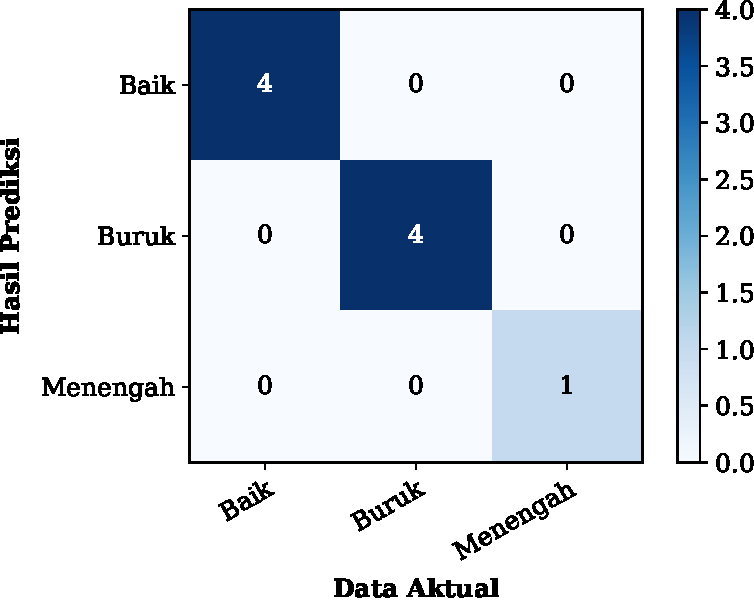
\includegraphics[width=0.6\textwidth]{BAB-4/plot/CM_selu_data_kecil.pdf}
		\captionof{figure}{Studi Kasus 2: \textit{Confusion Matrix} Menggunakan Fungsi Aktivasi \textit{Selu}}
		\label{gambar:CM selu layer DS-2}
	\end{minipage}
}

\centerline{\begin{minipage}{\linewidth}
		\centering
		\vspace{12 pt}
		%% Creator: Matplotlib, PGF backend
%%
%% To include the figure in your LaTeX document, write
%%   \input{<filename>.pgf}
%%
%% Make sure the required packages are loaded in your preamble
%%   \usepackage{pgf}
%%
%% Figures using additional raster images can only be included by \input if
%% they are in the same directory as the main LaTeX file. For loading figures
%% from other directories you can use the `import` package
%%   \usepackage{import}
%%
%% and then include the figures with
%%   \import{<path to file>}{<filename>.pgf}
%%
%% Matplotlib used the following preamble
%%
\begingroup%
\makeatletter%
\begin{pgfpicture}%
\pgfpathrectangle{\pgfpointorigin}{\pgfqpoint{5.640000in}{3.140000in}}%
\pgfusepath{use as bounding box, clip}%
\begin{pgfscope}%
\pgfsetbuttcap%
\pgfsetmiterjoin%
\pgfsetlinewidth{0.000000pt}%
\definecolor{currentstroke}{rgb}{1.000000,1.000000,1.000000}%
\pgfsetstrokecolor{currentstroke}%
\pgfsetstrokeopacity{0.000000}%
\pgfsetdash{}{0pt}%
\pgfpathmoveto{\pgfqpoint{0.000000in}{0.000000in}}%
\pgfpathlineto{\pgfqpoint{5.640000in}{0.000000in}}%
\pgfpathlineto{\pgfqpoint{5.640000in}{3.140000in}}%
\pgfpathlineto{\pgfqpoint{0.000000in}{3.140000in}}%
\pgfpathclose%
\pgfusepath{}%
\end{pgfscope}%
\begin{pgfscope}%
\pgfsetbuttcap%
\pgfsetmiterjoin%
\definecolor{currentfill}{rgb}{1.000000,1.000000,1.000000}%
\pgfsetfillcolor{currentfill}%
\pgfsetlinewidth{0.000000pt}%
\definecolor{currentstroke}{rgb}{0.000000,0.000000,0.000000}%
\pgfsetstrokecolor{currentstroke}%
\pgfsetstrokeopacity{0.000000}%
\pgfsetdash{}{0pt}%
\pgfpathmoveto{\pgfqpoint{0.453704in}{0.693723in}}%
\pgfpathlineto{\pgfqpoint{2.730000in}{0.693723in}}%
\pgfpathlineto{\pgfqpoint{2.730000in}{3.140000in}}%
\pgfpathlineto{\pgfqpoint{0.453704in}{3.140000in}}%
\pgfpathclose%
\pgfusepath{fill}%
\end{pgfscope}%
\begin{pgfscope}%
\pgfpathrectangle{\pgfqpoint{0.453704in}{0.693723in}}{\pgfqpoint{2.276296in}{2.446277in}}%
\pgfusepath{clip}%
\pgfsetbuttcap%
\pgfsetmiterjoin%
\definecolor{currentfill}{rgb}{0.121569,0.466667,0.705882}%
\pgfsetfillcolor{currentfill}%
\pgfsetlinewidth{0.000000pt}%
\definecolor{currentstroke}{rgb}{0.000000,0.000000,0.000000}%
\pgfsetstrokecolor{currentstroke}%
\pgfsetstrokeopacity{0.000000}%
\pgfsetdash{}{0pt}%
\pgfpathmoveto{\pgfqpoint{0.557172in}{0.693723in}}%
\pgfpathlineto{\pgfqpoint{0.902065in}{0.693723in}}%
\pgfpathlineto{\pgfqpoint{0.902065in}{2.917611in}}%
\pgfpathlineto{\pgfqpoint{0.557172in}{2.917611in}}%
\pgfpathclose%
\pgfusepath{fill}%
\end{pgfscope}%
\begin{pgfscope}%
\pgfpathrectangle{\pgfqpoint{0.453704in}{0.693723in}}{\pgfqpoint{2.276296in}{2.446277in}}%
\pgfusepath{clip}%
\pgfsetbuttcap%
\pgfsetmiterjoin%
\definecolor{currentfill}{rgb}{0.121569,0.466667,0.705882}%
\pgfsetfillcolor{currentfill}%
\pgfsetlinewidth{0.000000pt}%
\definecolor{currentstroke}{rgb}{0.000000,0.000000,0.000000}%
\pgfsetstrokecolor{currentstroke}%
\pgfsetstrokeopacity{0.000000}%
\pgfsetdash{}{0pt}%
\pgfpathmoveto{\pgfqpoint{1.419405in}{0.693723in}}%
\pgfpathlineto{\pgfqpoint{1.764299in}{0.693723in}}%
\pgfpathlineto{\pgfqpoint{1.764299in}{2.917611in}}%
\pgfpathlineto{\pgfqpoint{1.419405in}{2.917611in}}%
\pgfpathclose%
\pgfusepath{fill}%
\end{pgfscope}%
\begin{pgfscope}%
\pgfpathrectangle{\pgfqpoint{0.453704in}{0.693723in}}{\pgfqpoint{2.276296in}{2.446277in}}%
\pgfusepath{clip}%
\pgfsetbuttcap%
\pgfsetmiterjoin%
\definecolor{currentfill}{rgb}{0.121569,0.466667,0.705882}%
\pgfsetfillcolor{currentfill}%
\pgfsetlinewidth{0.000000pt}%
\definecolor{currentstroke}{rgb}{0.000000,0.000000,0.000000}%
\pgfsetstrokecolor{currentstroke}%
\pgfsetstrokeopacity{0.000000}%
\pgfsetdash{}{0pt}%
\pgfpathmoveto{\pgfqpoint{2.281639in}{0.693723in}}%
\pgfpathlineto{\pgfqpoint{2.626532in}{0.693723in}}%
\pgfpathlineto{\pgfqpoint{2.626532in}{2.917611in}}%
\pgfpathlineto{\pgfqpoint{2.281639in}{2.917611in}}%
\pgfpathclose%
\pgfusepath{fill}%
\end{pgfscope}%
\begin{pgfscope}%
\pgfsetbuttcap%
\pgfsetroundjoin%
\definecolor{currentfill}{rgb}{0.000000,0.000000,0.000000}%
\pgfsetfillcolor{currentfill}%
\pgfsetlinewidth{0.803000pt}%
\definecolor{currentstroke}{rgb}{0.000000,0.000000,0.000000}%
\pgfsetstrokecolor{currentstroke}%
\pgfsetdash{}{0pt}%
\pgfsys@defobject{currentmarker}{\pgfqpoint{0.000000in}{-0.048611in}}{\pgfqpoint{0.000000in}{0.000000in}}{%
\pgfpathmoveto{\pgfqpoint{0.000000in}{0.000000in}}%
\pgfpathlineto{\pgfqpoint{0.000000in}{-0.048611in}}%
\pgfusepath{stroke,fill}%
}%
\begin{pgfscope}%
\pgfsys@transformshift{0.729619in}{0.693723in}%
\pgfsys@useobject{currentmarker}{}%
\end{pgfscope}%
\end{pgfscope}%
\begin{pgfscope}%
\definecolor{textcolor}{rgb}{0.000000,0.000000,0.000000}%
\pgfsetstrokecolor{textcolor}%
\pgfsetfillcolor{textcolor}%
\pgftext[x=0.729619in,y=0.596500in,right,top,rotate=30.000000]{\color{textcolor}\rmfamily\fontsize{10.000000}{12.000000}\selectfont Baik}%
\end{pgfscope}%
\begin{pgfscope}%
\pgfsetbuttcap%
\pgfsetroundjoin%
\definecolor{currentfill}{rgb}{0.000000,0.000000,0.000000}%
\pgfsetfillcolor{currentfill}%
\pgfsetlinewidth{0.803000pt}%
\definecolor{currentstroke}{rgb}{0.000000,0.000000,0.000000}%
\pgfsetstrokecolor{currentstroke}%
\pgfsetdash{}{0pt}%
\pgfsys@defobject{currentmarker}{\pgfqpoint{0.000000in}{-0.048611in}}{\pgfqpoint{0.000000in}{0.000000in}}{%
\pgfpathmoveto{\pgfqpoint{0.000000in}{0.000000in}}%
\pgfpathlineto{\pgfqpoint{0.000000in}{-0.048611in}}%
\pgfusepath{stroke,fill}%
}%
\begin{pgfscope}%
\pgfsys@transformshift{1.591852in}{0.693723in}%
\pgfsys@useobject{currentmarker}{}%
\end{pgfscope}%
\end{pgfscope}%
\begin{pgfscope}%
\definecolor{textcolor}{rgb}{0.000000,0.000000,0.000000}%
\pgfsetstrokecolor{textcolor}%
\pgfsetfillcolor{textcolor}%
\pgftext[x=1.591852in,y=0.596500in,right,top,rotate=30.000000]{\color{textcolor}\rmfamily\fontsize{10.000000}{12.000000}\selectfont Buruk}%
\end{pgfscope}%
\begin{pgfscope}%
\pgfsetbuttcap%
\pgfsetroundjoin%
\definecolor{currentfill}{rgb}{0.000000,0.000000,0.000000}%
\pgfsetfillcolor{currentfill}%
\pgfsetlinewidth{0.803000pt}%
\definecolor{currentstroke}{rgb}{0.000000,0.000000,0.000000}%
\pgfsetstrokecolor{currentstroke}%
\pgfsetdash{}{0pt}%
\pgfsys@defobject{currentmarker}{\pgfqpoint{0.000000in}{-0.048611in}}{\pgfqpoint{0.000000in}{0.000000in}}{%
\pgfpathmoveto{\pgfqpoint{0.000000in}{0.000000in}}%
\pgfpathlineto{\pgfqpoint{0.000000in}{-0.048611in}}%
\pgfusepath{stroke,fill}%
}%
\begin{pgfscope}%
\pgfsys@transformshift{2.454085in}{0.693723in}%
\pgfsys@useobject{currentmarker}{}%
\end{pgfscope}%
\end{pgfscope}%
\begin{pgfscope}%
\definecolor{textcolor}{rgb}{0.000000,0.000000,0.000000}%
\pgfsetstrokecolor{textcolor}%
\pgfsetfillcolor{textcolor}%
\pgftext[x=2.454085in,y=0.596500in,right,top,rotate=30.000000]{\color{textcolor}\rmfamily\fontsize{10.000000}{12.000000}\selectfont Menengah}%
\end{pgfscope}%
\begin{pgfscope}%
\definecolor{textcolor}{rgb}{0.000000,0.000000,0.000000}%
\pgfsetstrokecolor{textcolor}%
\pgfsetfillcolor{textcolor}%
\pgftext[x=1.591852in,y=0.123457in,,top]{\color{textcolor}\rmfamily\fontsize{10.000000}{12.000000}\selectfont Kategori}%
\end{pgfscope}%
\begin{pgfscope}%
\pgfsetbuttcap%
\pgfsetroundjoin%
\definecolor{currentfill}{rgb}{0.000000,0.000000,0.000000}%
\pgfsetfillcolor{currentfill}%
\pgfsetlinewidth{0.803000pt}%
\definecolor{currentstroke}{rgb}{0.000000,0.000000,0.000000}%
\pgfsetstrokecolor{currentstroke}%
\pgfsetdash{}{0pt}%
\pgfsys@defobject{currentmarker}{\pgfqpoint{-0.048611in}{0.000000in}}{\pgfqpoint{-0.000000in}{0.000000in}}{%
\pgfpathmoveto{\pgfqpoint{-0.000000in}{0.000000in}}%
\pgfpathlineto{\pgfqpoint{-0.048611in}{0.000000in}}%
\pgfusepath{stroke,fill}%
}%
\begin{pgfscope}%
\pgfsys@transformshift{0.453704in}{0.693723in}%
\pgfsys@useobject{currentmarker}{}%
\end{pgfscope}%
\end{pgfscope}%
\begin{pgfscope}%
\definecolor{textcolor}{rgb}{0.000000,0.000000,0.000000}%
\pgfsetstrokecolor{textcolor}%
\pgfsetfillcolor{textcolor}%
\pgftext[x=0.179012in, y=0.645497in, left, base]{\color{textcolor}\rmfamily\fontsize{10.000000}{12.000000}\selectfont \(\displaystyle {0.0}\)}%
\end{pgfscope}%
\begin{pgfscope}%
\pgfsetbuttcap%
\pgfsetroundjoin%
\definecolor{currentfill}{rgb}{0.000000,0.000000,0.000000}%
\pgfsetfillcolor{currentfill}%
\pgfsetlinewidth{0.803000pt}%
\definecolor{currentstroke}{rgb}{0.000000,0.000000,0.000000}%
\pgfsetstrokecolor{currentstroke}%
\pgfsetdash{}{0pt}%
\pgfsys@defobject{currentmarker}{\pgfqpoint{-0.048611in}{0.000000in}}{\pgfqpoint{-0.000000in}{0.000000in}}{%
\pgfpathmoveto{\pgfqpoint{-0.000000in}{0.000000in}}%
\pgfpathlineto{\pgfqpoint{-0.048611in}{0.000000in}}%
\pgfusepath{stroke,fill}%
}%
\begin{pgfscope}%
\pgfsys@transformshift{0.453704in}{1.138500in}%
\pgfsys@useobject{currentmarker}{}%
\end{pgfscope}%
\end{pgfscope}%
\begin{pgfscope}%
\definecolor{textcolor}{rgb}{0.000000,0.000000,0.000000}%
\pgfsetstrokecolor{textcolor}%
\pgfsetfillcolor{textcolor}%
\pgftext[x=0.179012in, y=1.090275in, left, base]{\color{textcolor}\rmfamily\fontsize{10.000000}{12.000000}\selectfont \(\displaystyle {0.2}\)}%
\end{pgfscope}%
\begin{pgfscope}%
\pgfsetbuttcap%
\pgfsetroundjoin%
\definecolor{currentfill}{rgb}{0.000000,0.000000,0.000000}%
\pgfsetfillcolor{currentfill}%
\pgfsetlinewidth{0.803000pt}%
\definecolor{currentstroke}{rgb}{0.000000,0.000000,0.000000}%
\pgfsetstrokecolor{currentstroke}%
\pgfsetdash{}{0pt}%
\pgfsys@defobject{currentmarker}{\pgfqpoint{-0.048611in}{0.000000in}}{\pgfqpoint{-0.000000in}{0.000000in}}{%
\pgfpathmoveto{\pgfqpoint{-0.000000in}{0.000000in}}%
\pgfpathlineto{\pgfqpoint{-0.048611in}{0.000000in}}%
\pgfusepath{stroke,fill}%
}%
\begin{pgfscope}%
\pgfsys@transformshift{0.453704in}{1.583278in}%
\pgfsys@useobject{currentmarker}{}%
\end{pgfscope}%
\end{pgfscope}%
\begin{pgfscope}%
\definecolor{textcolor}{rgb}{0.000000,0.000000,0.000000}%
\pgfsetstrokecolor{textcolor}%
\pgfsetfillcolor{textcolor}%
\pgftext[x=0.179012in, y=1.535053in, left, base]{\color{textcolor}\rmfamily\fontsize{10.000000}{12.000000}\selectfont \(\displaystyle {0.4}\)}%
\end{pgfscope}%
\begin{pgfscope}%
\pgfsetbuttcap%
\pgfsetroundjoin%
\definecolor{currentfill}{rgb}{0.000000,0.000000,0.000000}%
\pgfsetfillcolor{currentfill}%
\pgfsetlinewidth{0.803000pt}%
\definecolor{currentstroke}{rgb}{0.000000,0.000000,0.000000}%
\pgfsetstrokecolor{currentstroke}%
\pgfsetdash{}{0pt}%
\pgfsys@defobject{currentmarker}{\pgfqpoint{-0.048611in}{0.000000in}}{\pgfqpoint{-0.000000in}{0.000000in}}{%
\pgfpathmoveto{\pgfqpoint{-0.000000in}{0.000000in}}%
\pgfpathlineto{\pgfqpoint{-0.048611in}{0.000000in}}%
\pgfusepath{stroke,fill}%
}%
\begin{pgfscope}%
\pgfsys@transformshift{0.453704in}{2.028056in}%
\pgfsys@useobject{currentmarker}{}%
\end{pgfscope}%
\end{pgfscope}%
\begin{pgfscope}%
\definecolor{textcolor}{rgb}{0.000000,0.000000,0.000000}%
\pgfsetstrokecolor{textcolor}%
\pgfsetfillcolor{textcolor}%
\pgftext[x=0.179012in, y=1.979831in, left, base]{\color{textcolor}\rmfamily\fontsize{10.000000}{12.000000}\selectfont \(\displaystyle {0.6}\)}%
\end{pgfscope}%
\begin{pgfscope}%
\pgfsetbuttcap%
\pgfsetroundjoin%
\definecolor{currentfill}{rgb}{0.000000,0.000000,0.000000}%
\pgfsetfillcolor{currentfill}%
\pgfsetlinewidth{0.803000pt}%
\definecolor{currentstroke}{rgb}{0.000000,0.000000,0.000000}%
\pgfsetstrokecolor{currentstroke}%
\pgfsetdash{}{0pt}%
\pgfsys@defobject{currentmarker}{\pgfqpoint{-0.048611in}{0.000000in}}{\pgfqpoint{-0.000000in}{0.000000in}}{%
\pgfpathmoveto{\pgfqpoint{-0.000000in}{0.000000in}}%
\pgfpathlineto{\pgfqpoint{-0.048611in}{0.000000in}}%
\pgfusepath{stroke,fill}%
}%
\begin{pgfscope}%
\pgfsys@transformshift{0.453704in}{2.472833in}%
\pgfsys@useobject{currentmarker}{}%
\end{pgfscope}%
\end{pgfscope}%
\begin{pgfscope}%
\definecolor{textcolor}{rgb}{0.000000,0.000000,0.000000}%
\pgfsetstrokecolor{textcolor}%
\pgfsetfillcolor{textcolor}%
\pgftext[x=0.179012in, y=2.424608in, left, base]{\color{textcolor}\rmfamily\fontsize{10.000000}{12.000000}\selectfont \(\displaystyle {0.8}\)}%
\end{pgfscope}%
\begin{pgfscope}%
\pgfsetbuttcap%
\pgfsetroundjoin%
\definecolor{currentfill}{rgb}{0.000000,0.000000,0.000000}%
\pgfsetfillcolor{currentfill}%
\pgfsetlinewidth{0.803000pt}%
\definecolor{currentstroke}{rgb}{0.000000,0.000000,0.000000}%
\pgfsetstrokecolor{currentstroke}%
\pgfsetdash{}{0pt}%
\pgfsys@defobject{currentmarker}{\pgfqpoint{-0.048611in}{0.000000in}}{\pgfqpoint{-0.000000in}{0.000000in}}{%
\pgfpathmoveto{\pgfqpoint{-0.000000in}{0.000000in}}%
\pgfpathlineto{\pgfqpoint{-0.048611in}{0.000000in}}%
\pgfusepath{stroke,fill}%
}%
\begin{pgfscope}%
\pgfsys@transformshift{0.453704in}{2.917611in}%
\pgfsys@useobject{currentmarker}{}%
\end{pgfscope}%
\end{pgfscope}%
\begin{pgfscope}%
\definecolor{textcolor}{rgb}{0.000000,0.000000,0.000000}%
\pgfsetstrokecolor{textcolor}%
\pgfsetfillcolor{textcolor}%
\pgftext[x=0.179012in, y=2.869386in, left, base]{\color{textcolor}\rmfamily\fontsize{10.000000}{12.000000}\selectfont \(\displaystyle {1.0}\)}%
\end{pgfscope}%
\begin{pgfscope}%
\definecolor{textcolor}{rgb}{0.000000,0.000000,0.000000}%
\pgfsetstrokecolor{textcolor}%
\pgfsetfillcolor{textcolor}%
\pgftext[x=0.123457in,y=1.916861in,,bottom,rotate=90.000000]{\color{textcolor}\rmfamily\fontsize{10.000000}{12.000000}\selectfont Presisi}%
\end{pgfscope}%
\begin{pgfscope}%
\pgfsetrectcap%
\pgfsetmiterjoin%
\pgfsetlinewidth{0.803000pt}%
\definecolor{currentstroke}{rgb}{0.000000,0.000000,0.000000}%
\pgfsetstrokecolor{currentstroke}%
\pgfsetdash{}{0pt}%
\pgfpathmoveto{\pgfqpoint{0.453704in}{0.693723in}}%
\pgfpathlineto{\pgfqpoint{0.453704in}{3.140000in}}%
\pgfusepath{stroke}%
\end{pgfscope}%
\begin{pgfscope}%
\pgfsetrectcap%
\pgfsetmiterjoin%
\pgfsetlinewidth{0.803000pt}%
\definecolor{currentstroke}{rgb}{0.000000,0.000000,0.000000}%
\pgfsetstrokecolor{currentstroke}%
\pgfsetdash{}{0pt}%
\pgfpathmoveto{\pgfqpoint{2.730000in}{0.693723in}}%
\pgfpathlineto{\pgfqpoint{2.730000in}{3.140000in}}%
\pgfusepath{stroke}%
\end{pgfscope}%
\begin{pgfscope}%
\pgfsetrectcap%
\pgfsetmiterjoin%
\pgfsetlinewidth{0.803000pt}%
\definecolor{currentstroke}{rgb}{0.000000,0.000000,0.000000}%
\pgfsetstrokecolor{currentstroke}%
\pgfsetdash{}{0pt}%
\pgfpathmoveto{\pgfqpoint{0.453704in}{0.693723in}}%
\pgfpathlineto{\pgfqpoint{2.730000in}{0.693723in}}%
\pgfusepath{stroke}%
\end{pgfscope}%
\begin{pgfscope}%
\pgfsetrectcap%
\pgfsetmiterjoin%
\pgfsetlinewidth{0.803000pt}%
\definecolor{currentstroke}{rgb}{0.000000,0.000000,0.000000}%
\pgfsetstrokecolor{currentstroke}%
\pgfsetdash{}{0pt}%
\pgfpathmoveto{\pgfqpoint{0.453704in}{3.140000in}}%
\pgfpathlineto{\pgfqpoint{2.730000in}{3.140000in}}%
\pgfusepath{stroke}%
\end{pgfscope}%
\begin{pgfscope}%
\definecolor{textcolor}{rgb}{0.000000,0.000000,0.000000}%
\pgfsetstrokecolor{textcolor}%
\pgfsetfillcolor{textcolor}%
\pgftext[x=0.729619in,y=2.939850in,,bottom]{\color{textcolor}\rmfamily\fontsize{9.000000}{10.800000}\selectfont 1.0}%
\end{pgfscope}%
\begin{pgfscope}%
\definecolor{textcolor}{rgb}{0.000000,0.000000,0.000000}%
\pgfsetstrokecolor{textcolor}%
\pgfsetfillcolor{textcolor}%
\pgftext[x=1.591852in,y=2.939850in,,bottom]{\color{textcolor}\rmfamily\fontsize{9.000000}{10.800000}\selectfont 1.0}%
\end{pgfscope}%
\begin{pgfscope}%
\definecolor{textcolor}{rgb}{0.000000,0.000000,0.000000}%
\pgfsetstrokecolor{textcolor}%
\pgfsetfillcolor{textcolor}%
\pgftext[x=2.454085in,y=2.939850in,,bottom]{\color{textcolor}\rmfamily\fontsize{9.000000}{10.800000}\selectfont 1.0}%
\end{pgfscope}%
\begin{pgfscope}%
\pgfsetbuttcap%
\pgfsetmiterjoin%
\definecolor{currentfill}{rgb}{1.000000,1.000000,1.000000}%
\pgfsetfillcolor{currentfill}%
\pgfsetlinewidth{0.000000pt}%
\definecolor{currentstroke}{rgb}{0.000000,0.000000,0.000000}%
\pgfsetstrokecolor{currentstroke}%
\pgfsetstrokeopacity{0.000000}%
\pgfsetdash{}{0pt}%
\pgfpathmoveto{\pgfqpoint{3.363704in}{0.693723in}}%
\pgfpathlineto{\pgfqpoint{5.640000in}{0.693723in}}%
\pgfpathlineto{\pgfqpoint{5.640000in}{3.140000in}}%
\pgfpathlineto{\pgfqpoint{3.363704in}{3.140000in}}%
\pgfpathclose%
\pgfusepath{fill}%
\end{pgfscope}%
\begin{pgfscope}%
\pgfpathrectangle{\pgfqpoint{3.363704in}{0.693723in}}{\pgfqpoint{2.276296in}{2.446277in}}%
\pgfusepath{clip}%
\pgfsetbuttcap%
\pgfsetmiterjoin%
\definecolor{currentfill}{rgb}{1.000000,0.498039,0.054902}%
\pgfsetfillcolor{currentfill}%
\pgfsetlinewidth{0.000000pt}%
\definecolor{currentstroke}{rgb}{0.000000,0.000000,0.000000}%
\pgfsetstrokecolor{currentstroke}%
\pgfsetstrokeopacity{0.000000}%
\pgfsetdash{}{0pt}%
\pgfpathmoveto{\pgfqpoint{3.467172in}{0.693723in}}%
\pgfpathlineto{\pgfqpoint{3.812065in}{0.693723in}}%
\pgfpathlineto{\pgfqpoint{3.812065in}{2.917611in}}%
\pgfpathlineto{\pgfqpoint{3.467172in}{2.917611in}}%
\pgfpathclose%
\pgfusepath{fill}%
\end{pgfscope}%
\begin{pgfscope}%
\pgfpathrectangle{\pgfqpoint{3.363704in}{0.693723in}}{\pgfqpoint{2.276296in}{2.446277in}}%
\pgfusepath{clip}%
\pgfsetbuttcap%
\pgfsetmiterjoin%
\definecolor{currentfill}{rgb}{1.000000,0.498039,0.054902}%
\pgfsetfillcolor{currentfill}%
\pgfsetlinewidth{0.000000pt}%
\definecolor{currentstroke}{rgb}{0.000000,0.000000,0.000000}%
\pgfsetstrokecolor{currentstroke}%
\pgfsetstrokeopacity{0.000000}%
\pgfsetdash{}{0pt}%
\pgfpathmoveto{\pgfqpoint{4.329405in}{0.693723in}}%
\pgfpathlineto{\pgfqpoint{4.674299in}{0.693723in}}%
\pgfpathlineto{\pgfqpoint{4.674299in}{2.917611in}}%
\pgfpathlineto{\pgfqpoint{4.329405in}{2.917611in}}%
\pgfpathclose%
\pgfusepath{fill}%
\end{pgfscope}%
\begin{pgfscope}%
\pgfpathrectangle{\pgfqpoint{3.363704in}{0.693723in}}{\pgfqpoint{2.276296in}{2.446277in}}%
\pgfusepath{clip}%
\pgfsetbuttcap%
\pgfsetmiterjoin%
\definecolor{currentfill}{rgb}{1.000000,0.498039,0.054902}%
\pgfsetfillcolor{currentfill}%
\pgfsetlinewidth{0.000000pt}%
\definecolor{currentstroke}{rgb}{0.000000,0.000000,0.000000}%
\pgfsetstrokecolor{currentstroke}%
\pgfsetstrokeopacity{0.000000}%
\pgfsetdash{}{0pt}%
\pgfpathmoveto{\pgfqpoint{5.191639in}{0.693723in}}%
\pgfpathlineto{\pgfqpoint{5.536532in}{0.693723in}}%
\pgfpathlineto{\pgfqpoint{5.536532in}{2.917611in}}%
\pgfpathlineto{\pgfqpoint{5.191639in}{2.917611in}}%
\pgfpathclose%
\pgfusepath{fill}%
\end{pgfscope}%
\begin{pgfscope}%
\pgfsetbuttcap%
\pgfsetroundjoin%
\definecolor{currentfill}{rgb}{0.000000,0.000000,0.000000}%
\pgfsetfillcolor{currentfill}%
\pgfsetlinewidth{0.803000pt}%
\definecolor{currentstroke}{rgb}{0.000000,0.000000,0.000000}%
\pgfsetstrokecolor{currentstroke}%
\pgfsetdash{}{0pt}%
\pgfsys@defobject{currentmarker}{\pgfqpoint{0.000000in}{-0.048611in}}{\pgfqpoint{0.000000in}{0.000000in}}{%
\pgfpathmoveto{\pgfqpoint{0.000000in}{0.000000in}}%
\pgfpathlineto{\pgfqpoint{0.000000in}{-0.048611in}}%
\pgfusepath{stroke,fill}%
}%
\begin{pgfscope}%
\pgfsys@transformshift{3.639619in}{0.693723in}%
\pgfsys@useobject{currentmarker}{}%
\end{pgfscope}%
\end{pgfscope}%
\begin{pgfscope}%
\definecolor{textcolor}{rgb}{0.000000,0.000000,0.000000}%
\pgfsetstrokecolor{textcolor}%
\pgfsetfillcolor{textcolor}%
\pgftext[x=3.639619in,y=0.596500in,right,top,rotate=30.000000]{\color{textcolor}\rmfamily\fontsize{10.000000}{12.000000}\selectfont Baik}%
\end{pgfscope}%
\begin{pgfscope}%
\pgfsetbuttcap%
\pgfsetroundjoin%
\definecolor{currentfill}{rgb}{0.000000,0.000000,0.000000}%
\pgfsetfillcolor{currentfill}%
\pgfsetlinewidth{0.803000pt}%
\definecolor{currentstroke}{rgb}{0.000000,0.000000,0.000000}%
\pgfsetstrokecolor{currentstroke}%
\pgfsetdash{}{0pt}%
\pgfsys@defobject{currentmarker}{\pgfqpoint{0.000000in}{-0.048611in}}{\pgfqpoint{0.000000in}{0.000000in}}{%
\pgfpathmoveto{\pgfqpoint{0.000000in}{0.000000in}}%
\pgfpathlineto{\pgfqpoint{0.000000in}{-0.048611in}}%
\pgfusepath{stroke,fill}%
}%
\begin{pgfscope}%
\pgfsys@transformshift{4.501852in}{0.693723in}%
\pgfsys@useobject{currentmarker}{}%
\end{pgfscope}%
\end{pgfscope}%
\begin{pgfscope}%
\definecolor{textcolor}{rgb}{0.000000,0.000000,0.000000}%
\pgfsetstrokecolor{textcolor}%
\pgfsetfillcolor{textcolor}%
\pgftext[x=4.501852in,y=0.596500in,right,top,rotate=30.000000]{\color{textcolor}\rmfamily\fontsize{10.000000}{12.000000}\selectfont Buruk}%
\end{pgfscope}%
\begin{pgfscope}%
\pgfsetbuttcap%
\pgfsetroundjoin%
\definecolor{currentfill}{rgb}{0.000000,0.000000,0.000000}%
\pgfsetfillcolor{currentfill}%
\pgfsetlinewidth{0.803000pt}%
\definecolor{currentstroke}{rgb}{0.000000,0.000000,0.000000}%
\pgfsetstrokecolor{currentstroke}%
\pgfsetdash{}{0pt}%
\pgfsys@defobject{currentmarker}{\pgfqpoint{0.000000in}{-0.048611in}}{\pgfqpoint{0.000000in}{0.000000in}}{%
\pgfpathmoveto{\pgfqpoint{0.000000in}{0.000000in}}%
\pgfpathlineto{\pgfqpoint{0.000000in}{-0.048611in}}%
\pgfusepath{stroke,fill}%
}%
\begin{pgfscope}%
\pgfsys@transformshift{5.364085in}{0.693723in}%
\pgfsys@useobject{currentmarker}{}%
\end{pgfscope}%
\end{pgfscope}%
\begin{pgfscope}%
\definecolor{textcolor}{rgb}{0.000000,0.000000,0.000000}%
\pgfsetstrokecolor{textcolor}%
\pgfsetfillcolor{textcolor}%
\pgftext[x=5.364085in,y=0.596500in,right,top,rotate=30.000000]{\color{textcolor}\rmfamily\fontsize{10.000000}{12.000000}\selectfont Menengah}%
\end{pgfscope}%
\begin{pgfscope}%
\definecolor{textcolor}{rgb}{0.000000,0.000000,0.000000}%
\pgfsetstrokecolor{textcolor}%
\pgfsetfillcolor{textcolor}%
\pgftext[x=4.501852in,y=0.123457in,,top]{\color{textcolor}\rmfamily\fontsize{10.000000}{12.000000}\selectfont Kategori}%
\end{pgfscope}%
\begin{pgfscope}%
\pgfsetbuttcap%
\pgfsetroundjoin%
\definecolor{currentfill}{rgb}{0.000000,0.000000,0.000000}%
\pgfsetfillcolor{currentfill}%
\pgfsetlinewidth{0.803000pt}%
\definecolor{currentstroke}{rgb}{0.000000,0.000000,0.000000}%
\pgfsetstrokecolor{currentstroke}%
\pgfsetdash{}{0pt}%
\pgfsys@defobject{currentmarker}{\pgfqpoint{-0.048611in}{0.000000in}}{\pgfqpoint{-0.000000in}{0.000000in}}{%
\pgfpathmoveto{\pgfqpoint{-0.000000in}{0.000000in}}%
\pgfpathlineto{\pgfqpoint{-0.048611in}{0.000000in}}%
\pgfusepath{stroke,fill}%
}%
\begin{pgfscope}%
\pgfsys@transformshift{3.363704in}{0.693723in}%
\pgfsys@useobject{currentmarker}{}%
\end{pgfscope}%
\end{pgfscope}%
\begin{pgfscope}%
\definecolor{textcolor}{rgb}{0.000000,0.000000,0.000000}%
\pgfsetstrokecolor{textcolor}%
\pgfsetfillcolor{textcolor}%
\pgftext[x=3.089012in, y=0.645497in, left, base]{\color{textcolor}\rmfamily\fontsize{10.000000}{12.000000}\selectfont \(\displaystyle {0.0}\)}%
\end{pgfscope}%
\begin{pgfscope}%
\pgfsetbuttcap%
\pgfsetroundjoin%
\definecolor{currentfill}{rgb}{0.000000,0.000000,0.000000}%
\pgfsetfillcolor{currentfill}%
\pgfsetlinewidth{0.803000pt}%
\definecolor{currentstroke}{rgb}{0.000000,0.000000,0.000000}%
\pgfsetstrokecolor{currentstroke}%
\pgfsetdash{}{0pt}%
\pgfsys@defobject{currentmarker}{\pgfqpoint{-0.048611in}{0.000000in}}{\pgfqpoint{-0.000000in}{0.000000in}}{%
\pgfpathmoveto{\pgfqpoint{-0.000000in}{0.000000in}}%
\pgfpathlineto{\pgfqpoint{-0.048611in}{0.000000in}}%
\pgfusepath{stroke,fill}%
}%
\begin{pgfscope}%
\pgfsys@transformshift{3.363704in}{1.138500in}%
\pgfsys@useobject{currentmarker}{}%
\end{pgfscope}%
\end{pgfscope}%
\begin{pgfscope}%
\definecolor{textcolor}{rgb}{0.000000,0.000000,0.000000}%
\pgfsetstrokecolor{textcolor}%
\pgfsetfillcolor{textcolor}%
\pgftext[x=3.089012in, y=1.090275in, left, base]{\color{textcolor}\rmfamily\fontsize{10.000000}{12.000000}\selectfont \(\displaystyle {0.2}\)}%
\end{pgfscope}%
\begin{pgfscope}%
\pgfsetbuttcap%
\pgfsetroundjoin%
\definecolor{currentfill}{rgb}{0.000000,0.000000,0.000000}%
\pgfsetfillcolor{currentfill}%
\pgfsetlinewidth{0.803000pt}%
\definecolor{currentstroke}{rgb}{0.000000,0.000000,0.000000}%
\pgfsetstrokecolor{currentstroke}%
\pgfsetdash{}{0pt}%
\pgfsys@defobject{currentmarker}{\pgfqpoint{-0.048611in}{0.000000in}}{\pgfqpoint{-0.000000in}{0.000000in}}{%
\pgfpathmoveto{\pgfqpoint{-0.000000in}{0.000000in}}%
\pgfpathlineto{\pgfqpoint{-0.048611in}{0.000000in}}%
\pgfusepath{stroke,fill}%
}%
\begin{pgfscope}%
\pgfsys@transformshift{3.363704in}{1.583278in}%
\pgfsys@useobject{currentmarker}{}%
\end{pgfscope}%
\end{pgfscope}%
\begin{pgfscope}%
\definecolor{textcolor}{rgb}{0.000000,0.000000,0.000000}%
\pgfsetstrokecolor{textcolor}%
\pgfsetfillcolor{textcolor}%
\pgftext[x=3.089012in, y=1.535053in, left, base]{\color{textcolor}\rmfamily\fontsize{10.000000}{12.000000}\selectfont \(\displaystyle {0.4}\)}%
\end{pgfscope}%
\begin{pgfscope}%
\pgfsetbuttcap%
\pgfsetroundjoin%
\definecolor{currentfill}{rgb}{0.000000,0.000000,0.000000}%
\pgfsetfillcolor{currentfill}%
\pgfsetlinewidth{0.803000pt}%
\definecolor{currentstroke}{rgb}{0.000000,0.000000,0.000000}%
\pgfsetstrokecolor{currentstroke}%
\pgfsetdash{}{0pt}%
\pgfsys@defobject{currentmarker}{\pgfqpoint{-0.048611in}{0.000000in}}{\pgfqpoint{-0.000000in}{0.000000in}}{%
\pgfpathmoveto{\pgfqpoint{-0.000000in}{0.000000in}}%
\pgfpathlineto{\pgfqpoint{-0.048611in}{0.000000in}}%
\pgfusepath{stroke,fill}%
}%
\begin{pgfscope}%
\pgfsys@transformshift{3.363704in}{2.028056in}%
\pgfsys@useobject{currentmarker}{}%
\end{pgfscope}%
\end{pgfscope}%
\begin{pgfscope}%
\definecolor{textcolor}{rgb}{0.000000,0.000000,0.000000}%
\pgfsetstrokecolor{textcolor}%
\pgfsetfillcolor{textcolor}%
\pgftext[x=3.089012in, y=1.979831in, left, base]{\color{textcolor}\rmfamily\fontsize{10.000000}{12.000000}\selectfont \(\displaystyle {0.6}\)}%
\end{pgfscope}%
\begin{pgfscope}%
\pgfsetbuttcap%
\pgfsetroundjoin%
\definecolor{currentfill}{rgb}{0.000000,0.000000,0.000000}%
\pgfsetfillcolor{currentfill}%
\pgfsetlinewidth{0.803000pt}%
\definecolor{currentstroke}{rgb}{0.000000,0.000000,0.000000}%
\pgfsetstrokecolor{currentstroke}%
\pgfsetdash{}{0pt}%
\pgfsys@defobject{currentmarker}{\pgfqpoint{-0.048611in}{0.000000in}}{\pgfqpoint{-0.000000in}{0.000000in}}{%
\pgfpathmoveto{\pgfqpoint{-0.000000in}{0.000000in}}%
\pgfpathlineto{\pgfqpoint{-0.048611in}{0.000000in}}%
\pgfusepath{stroke,fill}%
}%
\begin{pgfscope}%
\pgfsys@transformshift{3.363704in}{2.472833in}%
\pgfsys@useobject{currentmarker}{}%
\end{pgfscope}%
\end{pgfscope}%
\begin{pgfscope}%
\definecolor{textcolor}{rgb}{0.000000,0.000000,0.000000}%
\pgfsetstrokecolor{textcolor}%
\pgfsetfillcolor{textcolor}%
\pgftext[x=3.089012in, y=2.424608in, left, base]{\color{textcolor}\rmfamily\fontsize{10.000000}{12.000000}\selectfont \(\displaystyle {0.8}\)}%
\end{pgfscope}%
\begin{pgfscope}%
\pgfsetbuttcap%
\pgfsetroundjoin%
\definecolor{currentfill}{rgb}{0.000000,0.000000,0.000000}%
\pgfsetfillcolor{currentfill}%
\pgfsetlinewidth{0.803000pt}%
\definecolor{currentstroke}{rgb}{0.000000,0.000000,0.000000}%
\pgfsetstrokecolor{currentstroke}%
\pgfsetdash{}{0pt}%
\pgfsys@defobject{currentmarker}{\pgfqpoint{-0.048611in}{0.000000in}}{\pgfqpoint{-0.000000in}{0.000000in}}{%
\pgfpathmoveto{\pgfqpoint{-0.000000in}{0.000000in}}%
\pgfpathlineto{\pgfqpoint{-0.048611in}{0.000000in}}%
\pgfusepath{stroke,fill}%
}%
\begin{pgfscope}%
\pgfsys@transformshift{3.363704in}{2.917611in}%
\pgfsys@useobject{currentmarker}{}%
\end{pgfscope}%
\end{pgfscope}%
\begin{pgfscope}%
\definecolor{textcolor}{rgb}{0.000000,0.000000,0.000000}%
\pgfsetstrokecolor{textcolor}%
\pgfsetfillcolor{textcolor}%
\pgftext[x=3.089012in, y=2.869386in, left, base]{\color{textcolor}\rmfamily\fontsize{10.000000}{12.000000}\selectfont \(\displaystyle {1.0}\)}%
\end{pgfscope}%
\begin{pgfscope}%
\definecolor{textcolor}{rgb}{0.000000,0.000000,0.000000}%
\pgfsetstrokecolor{textcolor}%
\pgfsetfillcolor{textcolor}%
\pgftext[x=3.033457in,y=1.916861in,,bottom,rotate=90.000000]{\color{textcolor}\rmfamily\fontsize{10.000000}{12.000000}\selectfont Sensitivity}%
\end{pgfscope}%
\begin{pgfscope}%
\pgfsetrectcap%
\pgfsetmiterjoin%
\pgfsetlinewidth{0.803000pt}%
\definecolor{currentstroke}{rgb}{0.000000,0.000000,0.000000}%
\pgfsetstrokecolor{currentstroke}%
\pgfsetdash{}{0pt}%
\pgfpathmoveto{\pgfqpoint{3.363704in}{0.693723in}}%
\pgfpathlineto{\pgfqpoint{3.363704in}{3.140000in}}%
\pgfusepath{stroke}%
\end{pgfscope}%
\begin{pgfscope}%
\pgfsetrectcap%
\pgfsetmiterjoin%
\pgfsetlinewidth{0.803000pt}%
\definecolor{currentstroke}{rgb}{0.000000,0.000000,0.000000}%
\pgfsetstrokecolor{currentstroke}%
\pgfsetdash{}{0pt}%
\pgfpathmoveto{\pgfqpoint{5.640000in}{0.693723in}}%
\pgfpathlineto{\pgfqpoint{5.640000in}{3.140000in}}%
\pgfusepath{stroke}%
\end{pgfscope}%
\begin{pgfscope}%
\pgfsetrectcap%
\pgfsetmiterjoin%
\pgfsetlinewidth{0.803000pt}%
\definecolor{currentstroke}{rgb}{0.000000,0.000000,0.000000}%
\pgfsetstrokecolor{currentstroke}%
\pgfsetdash{}{0pt}%
\pgfpathmoveto{\pgfqpoint{3.363704in}{0.693723in}}%
\pgfpathlineto{\pgfqpoint{5.640000in}{0.693723in}}%
\pgfusepath{stroke}%
\end{pgfscope}%
\begin{pgfscope}%
\pgfsetrectcap%
\pgfsetmiterjoin%
\pgfsetlinewidth{0.803000pt}%
\definecolor{currentstroke}{rgb}{0.000000,0.000000,0.000000}%
\pgfsetstrokecolor{currentstroke}%
\pgfsetdash{}{0pt}%
\pgfpathmoveto{\pgfqpoint{3.363704in}{3.140000in}}%
\pgfpathlineto{\pgfqpoint{5.640000in}{3.140000in}}%
\pgfusepath{stroke}%
\end{pgfscope}%
\begin{pgfscope}%
\definecolor{textcolor}{rgb}{0.000000,0.000000,0.000000}%
\pgfsetstrokecolor{textcolor}%
\pgfsetfillcolor{textcolor}%
\pgftext[x=3.639619in,y=2.939850in,,bottom]{\color{textcolor}\rmfamily\fontsize{9.000000}{10.800000}\selectfont 1.0}%
\end{pgfscope}%
\begin{pgfscope}%
\definecolor{textcolor}{rgb}{0.000000,0.000000,0.000000}%
\pgfsetstrokecolor{textcolor}%
\pgfsetfillcolor{textcolor}%
\pgftext[x=4.501852in,y=2.939850in,,bottom]{\color{textcolor}\rmfamily\fontsize{9.000000}{10.800000}\selectfont 1.0}%
\end{pgfscope}%
\begin{pgfscope}%
\definecolor{textcolor}{rgb}{0.000000,0.000000,0.000000}%
\pgfsetstrokecolor{textcolor}%
\pgfsetfillcolor{textcolor}%
\pgftext[x=5.364085in,y=2.939850in,,bottom]{\color{textcolor}\rmfamily\fontsize{9.000000}{10.800000}\selectfont 1.0}%
\end{pgfscope}%
\end{pgfpicture}%
\makeatother%
\endgroup%

		\captionof{figure}{Studi Kasus 2: Presisi dan Sensitivitas Percobaan Perubahan Layer}
		\label{gambar:presisi sensitivity selu data kecil}
\end{minipage}}

Peninjauan berdasarkan hasil percobaan yang disajikan pada Gambar \ref{gambar:CM selu layer DS-2} dan Gambar \ref{gambar:presisi sensitivity selu data kecil} dapat dilihat bahwa model sudah dapat mendiagnosis setiap kategori tanpa adanya kesalahan, dengan demikian berdasarkan pada studi kasus 1 dan 2 penggunaan fungsi aktivasi \textit{selu} lebih cocok digunakan dalam model LSTM untuk mendiagnosis indeks kesehatan transformator daya. Hal ini dapat terjadi karena berdasarkan persamaan \ref{func:selu}, pada penggunaan fungsi aktivasi \textit{selu} nilai terendahnya untuk x<0 akan mendekati -1.76 jika input yang diberikan mendekati negatif tak hingga dan \textit{output} akan linier terhadap \textit{input} dengan faktor pengali 1.05070098. Hal ini akan membuat \textit{output} pada rentang -1.76 sampai tak hingga. Pada model hasil keluaran berupa vektor dengan indeks kesehatan ditentukan oleh urutan nilai tertinggi dari vektor tersebut. Jika sebelumnya digunakan fungsi aktivasi \textit{sigmoid} akan ada beberapa nilai yang berada pada saturasi 1, akibatnya perangkingan akan sulit ditentukan dan bisa terjadi dalam satu vektor terdapat dua nilai tertinggi yang sama yang membuat hasil diagnosis menjadi salah. Maka model LSTM dengan menggunakan sebuah \textit{hidden layer} serta menggunakan fungsi aktivasi \textit{selu} merupakan model dengan arsitektur yang paling baik pada perancangan studi kasus 2.

\subsection{Perubahan Pembagian Data dengan Rasio 8:2}
Pada dasarnya percobaan ini merupakan percobaan lanjutan untuk mengetahui pengaruh rasio set data terhadap akurasi pada model LSTM pada studi kasus 2. Model yang yang digunakan pada percobaan ini merupakan model dengan jumlah \textit{hidden layer} tunggal serta menggunakan fungsi aktivasi \textit{selu}. percobaan dijalankan dengan iterasi sebanyak 30 kali. Hasil percobaan ini dapat dilihat pada Gambar \ref{gambar:perbandingan rasio data kecil} dan Gambar \ref{gambar:akurasi rasio selu data kecil} yang merupakan representasi dari nilai akurasi rata-rata dan persebaran data secara berurutan.


\centerline{\begin{minipage}{\linewidth}
		\vspace{12 pt}
		\centering
		%% Creator: Matplotlib, PGF backend
%%
%% To include the figure in your LaTeX document, write
%%   \input{<filename>.pgf}
%%
%% Make sure the required packages are loaded in your preamble
%%   \usepackage{pgf}
%%
%% Figures using additional raster images can only be included by \input if
%% they are in the same directory as the main LaTeX file. For loading figures
%% from other directories you can use the `import` package
%%   \usepackage{import}
%%
%% and then include the figures with
%%   \import{<path to file>}{<filename>.pgf}
%%
%% Matplotlib used the following preamble
%%
\begingroup%
\makeatletter%
\begin{pgfpicture}%
\pgfpathrectangle{\pgfpointorigin}{\pgfqpoint{2.999722in}{2.999722in}}%
\pgfusepath{use as bounding box, clip}%
\begin{pgfscope}%
\pgfsetbuttcap%
\pgfsetmiterjoin%
\pgfsetlinewidth{0.000000pt}%
\definecolor{currentstroke}{rgb}{1.000000,1.000000,1.000000}%
\pgfsetstrokecolor{currentstroke}%
\pgfsetstrokeopacity{0.000000}%
\pgfsetdash{}{0pt}%
\pgfpathmoveto{\pgfqpoint{0.000000in}{0.000000in}}%
\pgfpathlineto{\pgfqpoint{2.999722in}{0.000000in}}%
\pgfpathlineto{\pgfqpoint{2.999722in}{2.999722in}}%
\pgfpathlineto{\pgfqpoint{0.000000in}{2.999722in}}%
\pgfpathclose%
\pgfusepath{}%
\end{pgfscope}%
\begin{pgfscope}%
\pgfsetbuttcap%
\pgfsetmiterjoin%
\definecolor{currentfill}{rgb}{1.000000,1.000000,1.000000}%
\pgfsetfillcolor{currentfill}%
\pgfsetlinewidth{0.000000pt}%
\definecolor{currentstroke}{rgb}{0.000000,0.000000,0.000000}%
\pgfsetstrokecolor{currentstroke}%
\pgfsetstrokeopacity{0.000000}%
\pgfsetdash{}{0pt}%
\pgfpathmoveto{\pgfqpoint{0.453704in}{0.527759in}}%
\pgfpathlineto{\pgfqpoint{2.999722in}{0.527759in}}%
\pgfpathlineto{\pgfqpoint{2.999722in}{2.999722in}}%
\pgfpathlineto{\pgfqpoint{0.453704in}{2.999722in}}%
\pgfpathclose%
\pgfusepath{fill}%
\end{pgfscope}%
\begin{pgfscope}%
\pgfpathrectangle{\pgfqpoint{0.453704in}{0.527759in}}{\pgfqpoint{2.546018in}{2.471963in}}%
\pgfusepath{clip}%
\pgfsetbuttcap%
\pgfsetmiterjoin%
\definecolor{currentfill}{rgb}{0.121569,0.466667,0.705882}%
\pgfsetfillcolor{currentfill}%
\pgfsetlinewidth{0.000000pt}%
\definecolor{currentstroke}{rgb}{0.000000,0.000000,0.000000}%
\pgfsetstrokecolor{currentstroke}%
\pgfsetstrokeopacity{0.000000}%
\pgfsetdash{}{0pt}%
\pgfpathmoveto{\pgfqpoint{0.569432in}{-0.993448in}}%
\pgfpathlineto{\pgfqpoint{1.726713in}{-0.993448in}}%
\pgfpathlineto{\pgfqpoint{1.726713in}{2.455890in}}%
\pgfpathlineto{\pgfqpoint{0.569432in}{2.455890in}}%
\pgfpathclose%
\pgfusepath{fill}%
\end{pgfscope}%
\begin{pgfscope}%
\pgfpathrectangle{\pgfqpoint{0.453704in}{0.527759in}}{\pgfqpoint{2.546018in}{2.471963in}}%
\pgfusepath{clip}%
\pgfsetbuttcap%
\pgfsetmiterjoin%
\definecolor{currentfill}{rgb}{1.000000,0.498039,0.054902}%
\pgfsetfillcolor{currentfill}%
\pgfsetlinewidth{0.000000pt}%
\definecolor{currentstroke}{rgb}{0.000000,0.000000,0.000000}%
\pgfsetstrokecolor{currentstroke}%
\pgfsetstrokeopacity{0.000000}%
\pgfsetdash{}{0pt}%
\pgfpathmoveto{\pgfqpoint{1.726713in}{-0.993448in}}%
\pgfpathlineto{\pgfqpoint{2.883994in}{-0.993448in}}%
\pgfpathlineto{\pgfqpoint{2.883994in}{1.942483in}}%
\pgfpathlineto{\pgfqpoint{1.726713in}{1.942483in}}%
\pgfpathclose%
\pgfusepath{fill}%
\end{pgfscope}%
\begin{pgfscope}%
\pgfsetbuttcap%
\pgfsetroundjoin%
\definecolor{currentfill}{rgb}{0.000000,0.000000,0.000000}%
\pgfsetfillcolor{currentfill}%
\pgfsetlinewidth{0.803000pt}%
\definecolor{currentstroke}{rgb}{0.000000,0.000000,0.000000}%
\pgfsetstrokecolor{currentstroke}%
\pgfsetdash{}{0pt}%
\pgfsys@defobject{currentmarker}{\pgfqpoint{0.000000in}{-0.048611in}}{\pgfqpoint{0.000000in}{0.000000in}}{%
\pgfpathmoveto{\pgfqpoint{0.000000in}{0.000000in}}%
\pgfpathlineto{\pgfqpoint{0.000000in}{-0.048611in}}%
\pgfusepath{stroke,fill}%
}%
\begin{pgfscope}%
\pgfsys@transformshift{1.726713in}{0.527759in}%
\pgfsys@useobject{currentmarker}{}%
\end{pgfscope}%
\end{pgfscope}%
\begin{pgfscope}%
\definecolor{textcolor}{rgb}{0.000000,0.000000,0.000000}%
\pgfsetstrokecolor{textcolor}%
\pgfsetfillcolor{textcolor}%
\pgftext[x=1.726713in,y=0.430537in,right,top,rotate=45.000000]{\color{textcolor}\rmfamily\fontsize{10.000000}{12.000000}\selectfont selu}%
\end{pgfscope}%
\begin{pgfscope}%
\definecolor{textcolor}{rgb}{0.000000,0.000000,0.000000}%
\pgfsetstrokecolor{textcolor}%
\pgfsetfillcolor{textcolor}%
\pgftext[x=1.726713in,y=0.123457in,,top]{\color{textcolor}\rmfamily\fontsize{10.000000}{12.000000}\selectfont Fungsi Aktivasi}%
\end{pgfscope}%
\begin{pgfscope}%
\pgfsetbuttcap%
\pgfsetroundjoin%
\definecolor{currentfill}{rgb}{0.000000,0.000000,0.000000}%
\pgfsetfillcolor{currentfill}%
\pgfsetlinewidth{0.803000pt}%
\definecolor{currentstroke}{rgb}{0.000000,0.000000,0.000000}%
\pgfsetstrokecolor{currentstroke}%
\pgfsetdash{}{0pt}%
\pgfsys@defobject{currentmarker}{\pgfqpoint{-0.048611in}{0.000000in}}{\pgfqpoint{-0.000000in}{0.000000in}}{%
\pgfpathmoveto{\pgfqpoint{-0.000000in}{0.000000in}}%
\pgfpathlineto{\pgfqpoint{-0.048611in}{0.000000in}}%
\pgfusepath{stroke,fill}%
}%
\begin{pgfscope}%
\pgfsys@transformshift{0.453704in}{0.527759in}%
\pgfsys@useobject{currentmarker}{}%
\end{pgfscope}%
\end{pgfscope}%
\begin{pgfscope}%
\definecolor{textcolor}{rgb}{0.000000,0.000000,0.000000}%
\pgfsetstrokecolor{textcolor}%
\pgfsetfillcolor{textcolor}%
\pgftext[x=0.179012in, y=0.479534in, left, base]{\color{textcolor}\rmfamily\fontsize{10.000000}{12.000000}\selectfont \(\displaystyle {0.4}\)}%
\end{pgfscope}%
\begin{pgfscope}%
\pgfsetbuttcap%
\pgfsetroundjoin%
\definecolor{currentfill}{rgb}{0.000000,0.000000,0.000000}%
\pgfsetfillcolor{currentfill}%
\pgfsetlinewidth{0.803000pt}%
\definecolor{currentstroke}{rgb}{0.000000,0.000000,0.000000}%
\pgfsetstrokecolor{currentstroke}%
\pgfsetdash{}{0pt}%
\pgfsys@defobject{currentmarker}{\pgfqpoint{-0.048611in}{0.000000in}}{\pgfqpoint{-0.000000in}{0.000000in}}{%
\pgfpathmoveto{\pgfqpoint{-0.000000in}{0.000000in}}%
\pgfpathlineto{\pgfqpoint{-0.048611in}{0.000000in}}%
\pgfusepath{stroke,fill}%
}%
\begin{pgfscope}%
\pgfsys@transformshift{0.453704in}{0.908061in}%
\pgfsys@useobject{currentmarker}{}%
\end{pgfscope}%
\end{pgfscope}%
\begin{pgfscope}%
\definecolor{textcolor}{rgb}{0.000000,0.000000,0.000000}%
\pgfsetstrokecolor{textcolor}%
\pgfsetfillcolor{textcolor}%
\pgftext[x=0.179012in, y=0.859836in, left, base]{\color{textcolor}\rmfamily\fontsize{10.000000}{12.000000}\selectfont \(\displaystyle {0.5}\)}%
\end{pgfscope}%
\begin{pgfscope}%
\pgfsetbuttcap%
\pgfsetroundjoin%
\definecolor{currentfill}{rgb}{0.000000,0.000000,0.000000}%
\pgfsetfillcolor{currentfill}%
\pgfsetlinewidth{0.803000pt}%
\definecolor{currentstroke}{rgb}{0.000000,0.000000,0.000000}%
\pgfsetstrokecolor{currentstroke}%
\pgfsetdash{}{0pt}%
\pgfsys@defobject{currentmarker}{\pgfqpoint{-0.048611in}{0.000000in}}{\pgfqpoint{-0.000000in}{0.000000in}}{%
\pgfpathmoveto{\pgfqpoint{-0.000000in}{0.000000in}}%
\pgfpathlineto{\pgfqpoint{-0.048611in}{0.000000in}}%
\pgfusepath{stroke,fill}%
}%
\begin{pgfscope}%
\pgfsys@transformshift{0.453704in}{1.288363in}%
\pgfsys@useobject{currentmarker}{}%
\end{pgfscope}%
\end{pgfscope}%
\begin{pgfscope}%
\definecolor{textcolor}{rgb}{0.000000,0.000000,0.000000}%
\pgfsetstrokecolor{textcolor}%
\pgfsetfillcolor{textcolor}%
\pgftext[x=0.179012in, y=1.240138in, left, base]{\color{textcolor}\rmfamily\fontsize{10.000000}{12.000000}\selectfont \(\displaystyle {0.6}\)}%
\end{pgfscope}%
\begin{pgfscope}%
\pgfsetbuttcap%
\pgfsetroundjoin%
\definecolor{currentfill}{rgb}{0.000000,0.000000,0.000000}%
\pgfsetfillcolor{currentfill}%
\pgfsetlinewidth{0.803000pt}%
\definecolor{currentstroke}{rgb}{0.000000,0.000000,0.000000}%
\pgfsetstrokecolor{currentstroke}%
\pgfsetdash{}{0pt}%
\pgfsys@defobject{currentmarker}{\pgfqpoint{-0.048611in}{0.000000in}}{\pgfqpoint{-0.000000in}{0.000000in}}{%
\pgfpathmoveto{\pgfqpoint{-0.000000in}{0.000000in}}%
\pgfpathlineto{\pgfqpoint{-0.048611in}{0.000000in}}%
\pgfusepath{stroke,fill}%
}%
\begin{pgfscope}%
\pgfsys@transformshift{0.453704in}{1.668665in}%
\pgfsys@useobject{currentmarker}{}%
\end{pgfscope}%
\end{pgfscope}%
\begin{pgfscope}%
\definecolor{textcolor}{rgb}{0.000000,0.000000,0.000000}%
\pgfsetstrokecolor{textcolor}%
\pgfsetfillcolor{textcolor}%
\pgftext[x=0.179012in, y=1.620440in, left, base]{\color{textcolor}\rmfamily\fontsize{10.000000}{12.000000}\selectfont \(\displaystyle {0.7}\)}%
\end{pgfscope}%
\begin{pgfscope}%
\pgfsetbuttcap%
\pgfsetroundjoin%
\definecolor{currentfill}{rgb}{0.000000,0.000000,0.000000}%
\pgfsetfillcolor{currentfill}%
\pgfsetlinewidth{0.803000pt}%
\definecolor{currentstroke}{rgb}{0.000000,0.000000,0.000000}%
\pgfsetstrokecolor{currentstroke}%
\pgfsetdash{}{0pt}%
\pgfsys@defobject{currentmarker}{\pgfqpoint{-0.048611in}{0.000000in}}{\pgfqpoint{-0.000000in}{0.000000in}}{%
\pgfpathmoveto{\pgfqpoint{-0.000000in}{0.000000in}}%
\pgfpathlineto{\pgfqpoint{-0.048611in}{0.000000in}}%
\pgfusepath{stroke,fill}%
}%
\begin{pgfscope}%
\pgfsys@transformshift{0.453704in}{2.048967in}%
\pgfsys@useobject{currentmarker}{}%
\end{pgfscope}%
\end{pgfscope}%
\begin{pgfscope}%
\definecolor{textcolor}{rgb}{0.000000,0.000000,0.000000}%
\pgfsetstrokecolor{textcolor}%
\pgfsetfillcolor{textcolor}%
\pgftext[x=0.179012in, y=2.000742in, left, base]{\color{textcolor}\rmfamily\fontsize{10.000000}{12.000000}\selectfont \(\displaystyle {0.8}\)}%
\end{pgfscope}%
\begin{pgfscope}%
\pgfsetbuttcap%
\pgfsetroundjoin%
\definecolor{currentfill}{rgb}{0.000000,0.000000,0.000000}%
\pgfsetfillcolor{currentfill}%
\pgfsetlinewidth{0.803000pt}%
\definecolor{currentstroke}{rgb}{0.000000,0.000000,0.000000}%
\pgfsetstrokecolor{currentstroke}%
\pgfsetdash{}{0pt}%
\pgfsys@defobject{currentmarker}{\pgfqpoint{-0.048611in}{0.000000in}}{\pgfqpoint{-0.000000in}{0.000000in}}{%
\pgfpathmoveto{\pgfqpoint{-0.000000in}{0.000000in}}%
\pgfpathlineto{\pgfqpoint{-0.048611in}{0.000000in}}%
\pgfusepath{stroke,fill}%
}%
\begin{pgfscope}%
\pgfsys@transformshift{0.453704in}{2.429269in}%
\pgfsys@useobject{currentmarker}{}%
\end{pgfscope}%
\end{pgfscope}%
\begin{pgfscope}%
\definecolor{textcolor}{rgb}{0.000000,0.000000,0.000000}%
\pgfsetstrokecolor{textcolor}%
\pgfsetfillcolor{textcolor}%
\pgftext[x=0.179012in, y=2.381044in, left, base]{\color{textcolor}\rmfamily\fontsize{10.000000}{12.000000}\selectfont \(\displaystyle {0.9}\)}%
\end{pgfscope}%
\begin{pgfscope}%
\pgfsetbuttcap%
\pgfsetroundjoin%
\definecolor{currentfill}{rgb}{0.000000,0.000000,0.000000}%
\pgfsetfillcolor{currentfill}%
\pgfsetlinewidth{0.803000pt}%
\definecolor{currentstroke}{rgb}{0.000000,0.000000,0.000000}%
\pgfsetstrokecolor{currentstroke}%
\pgfsetdash{}{0pt}%
\pgfsys@defobject{currentmarker}{\pgfqpoint{-0.048611in}{0.000000in}}{\pgfqpoint{-0.000000in}{0.000000in}}{%
\pgfpathmoveto{\pgfqpoint{-0.000000in}{0.000000in}}%
\pgfpathlineto{\pgfqpoint{-0.048611in}{0.000000in}}%
\pgfusepath{stroke,fill}%
}%
\begin{pgfscope}%
\pgfsys@transformshift{0.453704in}{2.809571in}%
\pgfsys@useobject{currentmarker}{}%
\end{pgfscope}%
\end{pgfscope}%
\begin{pgfscope}%
\definecolor{textcolor}{rgb}{0.000000,0.000000,0.000000}%
\pgfsetstrokecolor{textcolor}%
\pgfsetfillcolor{textcolor}%
\pgftext[x=0.179012in, y=2.761346in, left, base]{\color{textcolor}\rmfamily\fontsize{10.000000}{12.000000}\selectfont \(\displaystyle {1.0}\)}%
\end{pgfscope}%
\begin{pgfscope}%
\definecolor{textcolor}{rgb}{0.000000,0.000000,0.000000}%
\pgfsetstrokecolor{textcolor}%
\pgfsetfillcolor{textcolor}%
\pgftext[x=0.123457in,y=1.763741in,,bottom,rotate=90.000000]{\color{textcolor}\rmfamily\fontsize{10.000000}{12.000000}\selectfont Akurasi}%
\end{pgfscope}%
\begin{pgfscope}%
\pgfpathrectangle{\pgfqpoint{0.453704in}{0.527759in}}{\pgfqpoint{2.546018in}{2.471963in}}%
\pgfusepath{clip}%
\pgfsetbuttcap%
\pgfsetroundjoin%
\pgfsetlinewidth{1.505625pt}%
\definecolor{currentstroke}{rgb}{0.000000,0.000000,0.000000}%
\pgfsetstrokecolor{currentstroke}%
\pgfsetdash{}{0pt}%
\pgfpathmoveto{\pgfqpoint{1.148073in}{2.174628in}}%
\pgfpathlineto{\pgfqpoint{1.148073in}{2.737153in}}%
\pgfusepath{stroke}%
\end{pgfscope}%
\begin{pgfscope}%
\pgfpathrectangle{\pgfqpoint{0.453704in}{0.527759in}}{\pgfqpoint{2.546018in}{2.471963in}}%
\pgfusepath{clip}%
\pgfsetbuttcap%
\pgfsetroundjoin%
\pgfsetlinewidth{1.505625pt}%
\definecolor{currentstroke}{rgb}{0.000000,0.000000,0.000000}%
\pgfsetstrokecolor{currentstroke}%
\pgfsetdash{}{0pt}%
\pgfpathmoveto{\pgfqpoint{2.305354in}{1.518652in}}%
\pgfpathlineto{\pgfqpoint{2.305354in}{2.366313in}}%
\pgfusepath{stroke}%
\end{pgfscope}%
\begin{pgfscope}%
\pgfsetrectcap%
\pgfsetmiterjoin%
\pgfsetlinewidth{0.803000pt}%
\definecolor{currentstroke}{rgb}{0.000000,0.000000,0.000000}%
\pgfsetstrokecolor{currentstroke}%
\pgfsetdash{}{0pt}%
\pgfpathmoveto{\pgfqpoint{0.453704in}{0.527759in}}%
\pgfpathlineto{\pgfqpoint{0.453704in}{2.999722in}}%
\pgfusepath{stroke}%
\end{pgfscope}%
\begin{pgfscope}%
\pgfsetrectcap%
\pgfsetmiterjoin%
\pgfsetlinewidth{0.803000pt}%
\definecolor{currentstroke}{rgb}{0.000000,0.000000,0.000000}%
\pgfsetstrokecolor{currentstroke}%
\pgfsetdash{}{0pt}%
\pgfpathmoveto{\pgfqpoint{2.999722in}{0.527759in}}%
\pgfpathlineto{\pgfqpoint{2.999722in}{2.999722in}}%
\pgfusepath{stroke}%
\end{pgfscope}%
\begin{pgfscope}%
\pgfsetrectcap%
\pgfsetmiterjoin%
\pgfsetlinewidth{0.803000pt}%
\definecolor{currentstroke}{rgb}{0.000000,0.000000,0.000000}%
\pgfsetstrokecolor{currentstroke}%
\pgfsetdash{}{0pt}%
\pgfpathmoveto{\pgfqpoint{0.453704in}{0.527759in}}%
\pgfpathlineto{\pgfqpoint{2.999722in}{0.527759in}}%
\pgfusepath{stroke}%
\end{pgfscope}%
\begin{pgfscope}%
\pgfsetrectcap%
\pgfsetmiterjoin%
\pgfsetlinewidth{0.803000pt}%
\definecolor{currentstroke}{rgb}{0.000000,0.000000,0.000000}%
\pgfsetstrokecolor{currentstroke}%
\pgfsetdash{}{0pt}%
\pgfpathmoveto{\pgfqpoint{0.453704in}{2.999722in}}%
\pgfpathlineto{\pgfqpoint{2.999722in}{2.999722in}}%
\pgfusepath{stroke}%
\end{pgfscope}%
\begin{pgfscope}%
\definecolor{textcolor}{rgb}{0.000000,0.000000,0.000000}%
\pgfsetstrokecolor{textcolor}%
\pgfsetfillcolor{textcolor}%
\pgftext[x=1.001087in, y=2.465342in, left, base,rotate=60.000000]{\color{textcolor}\rmfamily\fontsize{7.000000}{8.400000}\selectfont 0.907}%
\end{pgfscope}%
\begin{pgfscope}%
\definecolor{textcolor}{rgb}{0.000000,0.000000,0.000000}%
\pgfsetstrokecolor{textcolor}%
\pgfsetfillcolor{textcolor}%
\pgftext[x=2.384657in, y=1.951935in, left, base,rotate=60.000000]{\color{textcolor}\rmfamily\fontsize{7.000000}{8.400000}\selectfont 0.772}%
\end{pgfscope}%
\begin{pgfscope}%
\pgfsetbuttcap%
\pgfsetmiterjoin%
\definecolor{currentfill}{rgb}{1.000000,1.000000,1.000000}%
\pgfsetfillcolor{currentfill}%
\pgfsetfillopacity{0.800000}%
\pgfsetlinewidth{1.003750pt}%
\definecolor{currentstroke}{rgb}{0.800000,0.800000,0.800000}%
\pgfsetstrokecolor{currentstroke}%
\pgfsetstrokeopacity{0.800000}%
\pgfsetdash{}{0pt}%
\pgfpathmoveto{\pgfqpoint{2.146209in}{2.650803in}}%
\pgfpathlineto{\pgfqpoint{2.931667in}{2.650803in}}%
\pgfpathquadraticcurveto{\pgfqpoint{2.951111in}{2.650803in}}{\pgfqpoint{2.951111in}{2.670247in}}%
\pgfpathlineto{\pgfqpoint{2.951111in}{2.931667in}}%
\pgfpathquadraticcurveto{\pgfqpoint{2.951111in}{2.951111in}}{\pgfqpoint{2.931667in}{2.951111in}}%
\pgfpathlineto{\pgfqpoint{2.146209in}{2.951111in}}%
\pgfpathquadraticcurveto{\pgfqpoint{2.126765in}{2.951111in}}{\pgfqpoint{2.126765in}{2.931667in}}%
\pgfpathlineto{\pgfqpoint{2.126765in}{2.670247in}}%
\pgfpathquadraticcurveto{\pgfqpoint{2.126765in}{2.650803in}}{\pgfqpoint{2.146209in}{2.650803in}}%
\pgfpathclose%
\pgfusepath{stroke,fill}%
\end{pgfscope}%
\begin{pgfscope}%
\pgfsetbuttcap%
\pgfsetmiterjoin%
\definecolor{currentfill}{rgb}{0.121569,0.466667,0.705882}%
\pgfsetfillcolor{currentfill}%
\pgfsetlinewidth{0.000000pt}%
\definecolor{currentstroke}{rgb}{0.000000,0.000000,0.000000}%
\pgfsetstrokecolor{currentstroke}%
\pgfsetstrokeopacity{0.000000}%
\pgfsetdash{}{0pt}%
\pgfpathmoveto{\pgfqpoint{2.165654in}{2.844167in}}%
\pgfpathlineto{\pgfqpoint{2.360098in}{2.844167in}}%
\pgfpathlineto{\pgfqpoint{2.360098in}{2.912222in}}%
\pgfpathlineto{\pgfqpoint{2.165654in}{2.912222in}}%
\pgfpathclose%
\pgfusepath{fill}%
\end{pgfscope}%
\begin{pgfscope}%
\definecolor{textcolor}{rgb}{0.000000,0.000000,0.000000}%
\pgfsetstrokecolor{textcolor}%
\pgfsetfillcolor{textcolor}%
\pgftext[x=2.437876in,y=2.844167in,left,base]{\color{textcolor}\rmfamily\fontsize{7.000000}{8.400000}\selectfont pelatihan}%
\end{pgfscope}%
\begin{pgfscope}%
\pgfsetbuttcap%
\pgfsetmiterjoin%
\definecolor{currentfill}{rgb}{1.000000,0.498039,0.054902}%
\pgfsetfillcolor{currentfill}%
\pgfsetlinewidth{0.000000pt}%
\definecolor{currentstroke}{rgb}{0.000000,0.000000,0.000000}%
\pgfsetstrokecolor{currentstroke}%
\pgfsetstrokeopacity{0.000000}%
\pgfsetdash{}{0pt}%
\pgfpathmoveto{\pgfqpoint{2.165654in}{2.708596in}}%
\pgfpathlineto{\pgfqpoint{2.360098in}{2.708596in}}%
\pgfpathlineto{\pgfqpoint{2.360098in}{2.776651in}}%
\pgfpathlineto{\pgfqpoint{2.165654in}{2.776651in}}%
\pgfpathclose%
\pgfusepath{fill}%
\end{pgfscope}%
\begin{pgfscope}%
\definecolor{textcolor}{rgb}{0.000000,0.000000,0.000000}%
\pgfsetstrokecolor{textcolor}%
\pgfsetfillcolor{textcolor}%
\pgftext[x=2.437876in,y=2.708596in,left,base]{\color{textcolor}\rmfamily\fontsize{7.000000}{8.400000}\selectfont pengujian}%
\end{pgfscope}%
\end{pgfpicture}%
\makeatother%
\endgroup%

		\captionof{figure}{Studi Kasus 2: Akurasi Percobaan Menggunakan Rasio Data Pelatihan dan Pengujian 8:2}
		\label{gambar:perbandingan rasio data kecil}
\end{minipage}}

\centerline{\begin{minipage}{\linewidth}
		\centering
		\vspace{12 pt}
		%% Creator: Matplotlib, PGF backend
%%
%% To include the figure in your LaTeX document, write
%%   \input{<filename>.pgf}
%%
%% Make sure the required packages are loaded in your preamble
%%   \usepackage{pgf}
%%
%% Figures using additional raster images can only be included by \input if
%% they are in the same directory as the main LaTeX file. For loading figures
%% from other directories you can use the `import` package
%%   \usepackage{import}
%%
%% and then include the figures with
%%   \import{<path to file>}{<filename>.pgf}
%%
%% Matplotlib used the following preamble
%%
\begingroup%
\makeatletter%
\begin{pgfpicture}%
\pgfpathrectangle{\pgfpointorigin}{\pgfqpoint{5.994670in}{2.999722in}}%
\pgfusepath{use as bounding box, clip}%
\begin{pgfscope}%
\pgfsetbuttcap%
\pgfsetmiterjoin%
\pgfsetlinewidth{0.000000pt}%
\definecolor{currentstroke}{rgb}{1.000000,1.000000,1.000000}%
\pgfsetstrokecolor{currentstroke}%
\pgfsetstrokeopacity{0.000000}%
\pgfsetdash{}{0pt}%
\pgfpathmoveto{\pgfqpoint{0.000000in}{0.000000in}}%
\pgfpathlineto{\pgfqpoint{5.994670in}{0.000000in}}%
\pgfpathlineto{\pgfqpoint{5.994670in}{2.999722in}}%
\pgfpathlineto{\pgfqpoint{0.000000in}{2.999722in}}%
\pgfpathclose%
\pgfusepath{}%
\end{pgfscope}%
\begin{pgfscope}%
\pgfsetbuttcap%
\pgfsetmiterjoin%
\definecolor{currentfill}{rgb}{1.000000,1.000000,1.000000}%
\pgfsetfillcolor{currentfill}%
\pgfsetlinewidth{0.000000pt}%
\definecolor{currentstroke}{rgb}{0.000000,0.000000,0.000000}%
\pgfsetstrokecolor{currentstroke}%
\pgfsetstrokeopacity{0.000000}%
\pgfsetdash{}{0pt}%
\pgfpathmoveto{\pgfqpoint{0.453704in}{0.399691in}}%
\pgfpathlineto{\pgfqpoint{2.925510in}{0.399691in}}%
\pgfpathlineto{\pgfqpoint{2.925510in}{2.999722in}}%
\pgfpathlineto{\pgfqpoint{0.453704in}{2.999722in}}%
\pgfpathclose%
\pgfusepath{fill}%
\end{pgfscope}%
\begin{pgfscope}%
\pgfpathrectangle{\pgfqpoint{0.453704in}{0.399691in}}{\pgfqpoint{2.471806in}{2.600031in}}%
\pgfusepath{clip}%
\pgfsetbuttcap%
\pgfsetroundjoin%
\definecolor{currentfill}{rgb}{1.000000,0.000000,0.000000}%
\pgfsetfillcolor{currentfill}%
\pgfsetlinewidth{1.003750pt}%
\definecolor{currentstroke}{rgb}{1.000000,0.000000,0.000000}%
\pgfsetstrokecolor{currentstroke}%
\pgfsetdash{}{0pt}%
\pgfsys@defobject{currentmarker}{\pgfqpoint{-0.041667in}{-0.041667in}}{\pgfqpoint{0.041667in}{0.041667in}}{%
\pgfpathmoveto{\pgfqpoint{0.000000in}{-0.041667in}}%
\pgfpathcurveto{\pgfqpoint{0.011050in}{-0.041667in}}{\pgfqpoint{0.021649in}{-0.037276in}}{\pgfqpoint{0.029463in}{-0.029463in}}%
\pgfpathcurveto{\pgfqpoint{0.037276in}{-0.021649in}}{\pgfqpoint{0.041667in}{-0.011050in}}{\pgfqpoint{0.041667in}{0.000000in}}%
\pgfpathcurveto{\pgfqpoint{0.041667in}{0.011050in}}{\pgfqpoint{0.037276in}{0.021649in}}{\pgfqpoint{0.029463in}{0.029463in}}%
\pgfpathcurveto{\pgfqpoint{0.021649in}{0.037276in}}{\pgfqpoint{0.011050in}{0.041667in}}{\pgfqpoint{0.000000in}{0.041667in}}%
\pgfpathcurveto{\pgfqpoint{-0.011050in}{0.041667in}}{\pgfqpoint{-0.021649in}{0.037276in}}{\pgfqpoint{-0.029463in}{0.029463in}}%
\pgfpathcurveto{\pgfqpoint{-0.037276in}{0.021649in}}{\pgfqpoint{-0.041667in}{0.011050in}}{\pgfqpoint{-0.041667in}{0.000000in}}%
\pgfpathcurveto{\pgfqpoint{-0.041667in}{-0.011050in}}{\pgfqpoint{-0.037276in}{-0.021649in}}{\pgfqpoint{-0.029463in}{-0.029463in}}%
\pgfpathcurveto{\pgfqpoint{-0.021649in}{-0.037276in}}{\pgfqpoint{-0.011050in}{-0.041667in}}{\pgfqpoint{0.000000in}{-0.041667in}}%
\pgfpathclose%
\pgfusepath{stroke,fill}%
}%
\begin{pgfscope}%
\pgfsys@transformshift{0.566059in}{1.670818in}%
\pgfsys@useobject{currentmarker}{}%
\end{pgfscope}%
\begin{pgfscope}%
\pgfsys@transformshift{0.643545in}{2.331143in}%
\pgfsys@useobject{currentmarker}{}%
\end{pgfscope}%
\begin{pgfscope}%
\pgfsys@transformshift{0.721031in}{2.166061in}%
\pgfsys@useobject{currentmarker}{}%
\end{pgfscope}%
\begin{pgfscope}%
\pgfsys@transformshift{0.798517in}{2.000980in}%
\pgfsys@useobject{currentmarker}{}%
\end{pgfscope}%
\begin{pgfscope}%
\pgfsys@transformshift{0.876003in}{2.166061in}%
\pgfsys@useobject{currentmarker}{}%
\end{pgfscope}%
\begin{pgfscope}%
\pgfsys@transformshift{0.953489in}{2.331143in}%
\pgfsys@useobject{currentmarker}{}%
\end{pgfscope}%
\begin{pgfscope}%
\pgfsys@transformshift{1.030976in}{2.331143in}%
\pgfsys@useobject{currentmarker}{}%
\end{pgfscope}%
\begin{pgfscope}%
\pgfsys@transformshift{1.108462in}{2.331143in}%
\pgfsys@useobject{currentmarker}{}%
\end{pgfscope}%
\begin{pgfscope}%
\pgfsys@transformshift{1.185948in}{2.331143in}%
\pgfsys@useobject{currentmarker}{}%
\end{pgfscope}%
\begin{pgfscope}%
\pgfsys@transformshift{1.263434in}{2.166061in}%
\pgfsys@useobject{currentmarker}{}%
\end{pgfscope}%
\begin{pgfscope}%
\pgfsys@transformshift{1.340920in}{2.331143in}%
\pgfsys@useobject{currentmarker}{}%
\end{pgfscope}%
\begin{pgfscope}%
\pgfsys@transformshift{1.418406in}{1.835899in}%
\pgfsys@useobject{currentmarker}{}%
\end{pgfscope}%
\begin{pgfscope}%
\pgfsys@transformshift{1.495892in}{1.835899in}%
\pgfsys@useobject{currentmarker}{}%
\end{pgfscope}%
\begin{pgfscope}%
\pgfsys@transformshift{1.573378in}{2.166061in}%
\pgfsys@useobject{currentmarker}{}%
\end{pgfscope}%
\begin{pgfscope}%
\pgfsys@transformshift{1.650864in}{1.835899in}%
\pgfsys@useobject{currentmarker}{}%
\end{pgfscope}%
\begin{pgfscope}%
\pgfsys@transformshift{1.728350in}{2.166061in}%
\pgfsys@useobject{currentmarker}{}%
\end{pgfscope}%
\begin{pgfscope}%
\pgfsys@transformshift{1.805836in}{2.496224in}%
\pgfsys@useobject{currentmarker}{}%
\end{pgfscope}%
\begin{pgfscope}%
\pgfsys@transformshift{1.883323in}{2.496224in}%
\pgfsys@useobject{currentmarker}{}%
\end{pgfscope}%
\begin{pgfscope}%
\pgfsys@transformshift{1.960809in}{2.166061in}%
\pgfsys@useobject{currentmarker}{}%
\end{pgfscope}%
\begin{pgfscope}%
\pgfsys@transformshift{2.038295in}{2.331143in}%
\pgfsys@useobject{currentmarker}{}%
\end{pgfscope}%
\begin{pgfscope}%
\pgfsys@transformshift{2.115781in}{2.496224in}%
\pgfsys@useobject{currentmarker}{}%
\end{pgfscope}%
\begin{pgfscope}%
\pgfsys@transformshift{2.193267in}{2.166061in}%
\pgfsys@useobject{currentmarker}{}%
\end{pgfscope}%
\begin{pgfscope}%
\pgfsys@transformshift{2.270753in}{2.000980in}%
\pgfsys@useobject{currentmarker}{}%
\end{pgfscope}%
\begin{pgfscope}%
\pgfsys@transformshift{2.348239in}{2.496224in}%
\pgfsys@useobject{currentmarker}{}%
\end{pgfscope}%
\begin{pgfscope}%
\pgfsys@transformshift{2.425725in}{2.166061in}%
\pgfsys@useobject{currentmarker}{}%
\end{pgfscope}%
\begin{pgfscope}%
\pgfsys@transformshift{2.503211in}{1.835899in}%
\pgfsys@useobject{currentmarker}{}%
\end{pgfscope}%
\begin{pgfscope}%
\pgfsys@transformshift{2.580697in}{2.166061in}%
\pgfsys@useobject{currentmarker}{}%
\end{pgfscope}%
\begin{pgfscope}%
\pgfsys@transformshift{2.658183in}{2.496224in}%
\pgfsys@useobject{currentmarker}{}%
\end{pgfscope}%
\begin{pgfscope}%
\pgfsys@transformshift{2.735670in}{2.166061in}%
\pgfsys@useobject{currentmarker}{}%
\end{pgfscope}%
\begin{pgfscope}%
\pgfsys@transformshift{2.813156in}{2.331143in}%
\pgfsys@useobject{currentmarker}{}%
\end{pgfscope}%
\end{pgfscope}%
\begin{pgfscope}%
\pgfsetbuttcap%
\pgfsetroundjoin%
\definecolor{currentfill}{rgb}{0.000000,0.000000,0.000000}%
\pgfsetfillcolor{currentfill}%
\pgfsetlinewidth{0.803000pt}%
\definecolor{currentstroke}{rgb}{0.000000,0.000000,0.000000}%
\pgfsetstrokecolor{currentstroke}%
\pgfsetdash{}{0pt}%
\pgfsys@defobject{currentmarker}{\pgfqpoint{0.000000in}{-0.048611in}}{\pgfqpoint{0.000000in}{0.000000in}}{%
\pgfpathmoveto{\pgfqpoint{0.000000in}{0.000000in}}%
\pgfpathlineto{\pgfqpoint{0.000000in}{-0.048611in}}%
\pgfusepath{stroke,fill}%
}%
\begin{pgfscope}%
\pgfsys@transformshift{0.566059in}{0.399691in}%
\pgfsys@useobject{currentmarker}{}%
\end{pgfscope}%
\end{pgfscope}%
\begin{pgfscope}%
\definecolor{textcolor}{rgb}{0.000000,0.000000,0.000000}%
\pgfsetstrokecolor{textcolor}%
\pgfsetfillcolor{textcolor}%
\pgftext[x=0.566059in,y=0.302469in,,top]{\color{textcolor}\rmfamily\fontsize{10.000000}{12.000000}\selectfont \(\displaystyle {0}\)}%
\end{pgfscope}%
\begin{pgfscope}%
\pgfsetbuttcap%
\pgfsetroundjoin%
\definecolor{currentfill}{rgb}{0.000000,0.000000,0.000000}%
\pgfsetfillcolor{currentfill}%
\pgfsetlinewidth{0.803000pt}%
\definecolor{currentstroke}{rgb}{0.000000,0.000000,0.000000}%
\pgfsetstrokecolor{currentstroke}%
\pgfsetdash{}{0pt}%
\pgfsys@defobject{currentmarker}{\pgfqpoint{0.000000in}{-0.048611in}}{\pgfqpoint{0.000000in}{0.000000in}}{%
\pgfpathmoveto{\pgfqpoint{0.000000in}{0.000000in}}%
\pgfpathlineto{\pgfqpoint{0.000000in}{-0.048611in}}%
\pgfusepath{stroke,fill}%
}%
\begin{pgfscope}%
\pgfsys@transformshift{1.340920in}{0.399691in}%
\pgfsys@useobject{currentmarker}{}%
\end{pgfscope}%
\end{pgfscope}%
\begin{pgfscope}%
\definecolor{textcolor}{rgb}{0.000000,0.000000,0.000000}%
\pgfsetstrokecolor{textcolor}%
\pgfsetfillcolor{textcolor}%
\pgftext[x=1.340920in,y=0.302469in,,top]{\color{textcolor}\rmfamily\fontsize{10.000000}{12.000000}\selectfont \(\displaystyle {10}\)}%
\end{pgfscope}%
\begin{pgfscope}%
\pgfsetbuttcap%
\pgfsetroundjoin%
\definecolor{currentfill}{rgb}{0.000000,0.000000,0.000000}%
\pgfsetfillcolor{currentfill}%
\pgfsetlinewidth{0.803000pt}%
\definecolor{currentstroke}{rgb}{0.000000,0.000000,0.000000}%
\pgfsetstrokecolor{currentstroke}%
\pgfsetdash{}{0pt}%
\pgfsys@defobject{currentmarker}{\pgfqpoint{0.000000in}{-0.048611in}}{\pgfqpoint{0.000000in}{0.000000in}}{%
\pgfpathmoveto{\pgfqpoint{0.000000in}{0.000000in}}%
\pgfpathlineto{\pgfqpoint{0.000000in}{-0.048611in}}%
\pgfusepath{stroke,fill}%
}%
\begin{pgfscope}%
\pgfsys@transformshift{2.115781in}{0.399691in}%
\pgfsys@useobject{currentmarker}{}%
\end{pgfscope}%
\end{pgfscope}%
\begin{pgfscope}%
\definecolor{textcolor}{rgb}{0.000000,0.000000,0.000000}%
\pgfsetstrokecolor{textcolor}%
\pgfsetfillcolor{textcolor}%
\pgftext[x=2.115781in,y=0.302469in,,top]{\color{textcolor}\rmfamily\fontsize{10.000000}{12.000000}\selectfont \(\displaystyle {20}\)}%
\end{pgfscope}%
\begin{pgfscope}%
\pgfsetbuttcap%
\pgfsetroundjoin%
\definecolor{currentfill}{rgb}{0.000000,0.000000,0.000000}%
\pgfsetfillcolor{currentfill}%
\pgfsetlinewidth{0.803000pt}%
\definecolor{currentstroke}{rgb}{0.000000,0.000000,0.000000}%
\pgfsetstrokecolor{currentstroke}%
\pgfsetdash{}{0pt}%
\pgfsys@defobject{currentmarker}{\pgfqpoint{0.000000in}{-0.048611in}}{\pgfqpoint{0.000000in}{0.000000in}}{%
\pgfpathmoveto{\pgfqpoint{0.000000in}{0.000000in}}%
\pgfpathlineto{\pgfqpoint{0.000000in}{-0.048611in}}%
\pgfusepath{stroke,fill}%
}%
\begin{pgfscope}%
\pgfsys@transformshift{2.890642in}{0.399691in}%
\pgfsys@useobject{currentmarker}{}%
\end{pgfscope}%
\end{pgfscope}%
\begin{pgfscope}%
\definecolor{textcolor}{rgb}{0.000000,0.000000,0.000000}%
\pgfsetstrokecolor{textcolor}%
\pgfsetfillcolor{textcolor}%
\pgftext[x=2.890642in,y=0.302469in,,top]{\color{textcolor}\rmfamily\fontsize{10.000000}{12.000000}\selectfont \(\displaystyle {30}\)}%
\end{pgfscope}%
\begin{pgfscope}%
\definecolor{textcolor}{rgb}{0.000000,0.000000,0.000000}%
\pgfsetstrokecolor{textcolor}%
\pgfsetfillcolor{textcolor}%
\pgftext[x=1.689607in,y=0.123457in,,top]{\color{textcolor}\rmfamily\fontsize{10.000000}{12.000000}\selectfont Iterasi Percobaan}%
\end{pgfscope}%
\begin{pgfscope}%
\pgfsetbuttcap%
\pgfsetroundjoin%
\definecolor{currentfill}{rgb}{0.000000,0.000000,0.000000}%
\pgfsetfillcolor{currentfill}%
\pgfsetlinewidth{0.803000pt}%
\definecolor{currentstroke}{rgb}{0.000000,0.000000,0.000000}%
\pgfsetstrokecolor{currentstroke}%
\pgfsetdash{}{0pt}%
\pgfsys@defobject{currentmarker}{\pgfqpoint{-0.048611in}{0.000000in}}{\pgfqpoint{-0.000000in}{0.000000in}}{%
\pgfpathmoveto{\pgfqpoint{-0.000000in}{0.000000in}}%
\pgfpathlineto{\pgfqpoint{-0.048611in}{0.000000in}}%
\pgfusepath{stroke,fill}%
}%
\begin{pgfscope}%
\pgfsys@transformshift{0.453704in}{0.399691in}%
\pgfsys@useobject{currentmarker}{}%
\end{pgfscope}%
\end{pgfscope}%
\begin{pgfscope}%
\definecolor{textcolor}{rgb}{0.000000,0.000000,0.000000}%
\pgfsetstrokecolor{textcolor}%
\pgfsetfillcolor{textcolor}%
\pgftext[x=0.179012in, y=0.351466in, left, base]{\color{textcolor}\rmfamily\fontsize{10.000000}{12.000000}\selectfont \(\displaystyle {0.3}\)}%
\end{pgfscope}%
\begin{pgfscope}%
\pgfsetbuttcap%
\pgfsetroundjoin%
\definecolor{currentfill}{rgb}{0.000000,0.000000,0.000000}%
\pgfsetfillcolor{currentfill}%
\pgfsetlinewidth{0.803000pt}%
\definecolor{currentstroke}{rgb}{0.000000,0.000000,0.000000}%
\pgfsetstrokecolor{currentstroke}%
\pgfsetdash{}{0pt}%
\pgfsys@defobject{currentmarker}{\pgfqpoint{-0.048611in}{0.000000in}}{\pgfqpoint{-0.000000in}{0.000000in}}{%
\pgfpathmoveto{\pgfqpoint{-0.000000in}{0.000000in}}%
\pgfpathlineto{\pgfqpoint{-0.048611in}{0.000000in}}%
\pgfusepath{stroke,fill}%
}%
\begin{pgfscope}%
\pgfsys@transformshift{0.453704in}{0.746362in}%
\pgfsys@useobject{currentmarker}{}%
\end{pgfscope}%
\end{pgfscope}%
\begin{pgfscope}%
\definecolor{textcolor}{rgb}{0.000000,0.000000,0.000000}%
\pgfsetstrokecolor{textcolor}%
\pgfsetfillcolor{textcolor}%
\pgftext[x=0.179012in, y=0.698137in, left, base]{\color{textcolor}\rmfamily\fontsize{10.000000}{12.000000}\selectfont \(\displaystyle {0.4}\)}%
\end{pgfscope}%
\begin{pgfscope}%
\pgfsetbuttcap%
\pgfsetroundjoin%
\definecolor{currentfill}{rgb}{0.000000,0.000000,0.000000}%
\pgfsetfillcolor{currentfill}%
\pgfsetlinewidth{0.803000pt}%
\definecolor{currentstroke}{rgb}{0.000000,0.000000,0.000000}%
\pgfsetstrokecolor{currentstroke}%
\pgfsetdash{}{0pt}%
\pgfsys@defobject{currentmarker}{\pgfqpoint{-0.048611in}{0.000000in}}{\pgfqpoint{-0.000000in}{0.000000in}}{%
\pgfpathmoveto{\pgfqpoint{-0.000000in}{0.000000in}}%
\pgfpathlineto{\pgfqpoint{-0.048611in}{0.000000in}}%
\pgfusepath{stroke,fill}%
}%
\begin{pgfscope}%
\pgfsys@transformshift{0.453704in}{1.093033in}%
\pgfsys@useobject{currentmarker}{}%
\end{pgfscope}%
\end{pgfscope}%
\begin{pgfscope}%
\definecolor{textcolor}{rgb}{0.000000,0.000000,0.000000}%
\pgfsetstrokecolor{textcolor}%
\pgfsetfillcolor{textcolor}%
\pgftext[x=0.179012in, y=1.044807in, left, base]{\color{textcolor}\rmfamily\fontsize{10.000000}{12.000000}\selectfont \(\displaystyle {0.5}\)}%
\end{pgfscope}%
\begin{pgfscope}%
\pgfsetbuttcap%
\pgfsetroundjoin%
\definecolor{currentfill}{rgb}{0.000000,0.000000,0.000000}%
\pgfsetfillcolor{currentfill}%
\pgfsetlinewidth{0.803000pt}%
\definecolor{currentstroke}{rgb}{0.000000,0.000000,0.000000}%
\pgfsetstrokecolor{currentstroke}%
\pgfsetdash{}{0pt}%
\pgfsys@defobject{currentmarker}{\pgfqpoint{-0.048611in}{0.000000in}}{\pgfqpoint{-0.000000in}{0.000000in}}{%
\pgfpathmoveto{\pgfqpoint{-0.000000in}{0.000000in}}%
\pgfpathlineto{\pgfqpoint{-0.048611in}{0.000000in}}%
\pgfusepath{stroke,fill}%
}%
\begin{pgfscope}%
\pgfsys@transformshift{0.453704in}{1.439704in}%
\pgfsys@useobject{currentmarker}{}%
\end{pgfscope}%
\end{pgfscope}%
\begin{pgfscope}%
\definecolor{textcolor}{rgb}{0.000000,0.000000,0.000000}%
\pgfsetstrokecolor{textcolor}%
\pgfsetfillcolor{textcolor}%
\pgftext[x=0.179012in, y=1.391478in, left, base]{\color{textcolor}\rmfamily\fontsize{10.000000}{12.000000}\selectfont \(\displaystyle {0.6}\)}%
\end{pgfscope}%
\begin{pgfscope}%
\pgfsetbuttcap%
\pgfsetroundjoin%
\definecolor{currentfill}{rgb}{0.000000,0.000000,0.000000}%
\pgfsetfillcolor{currentfill}%
\pgfsetlinewidth{0.803000pt}%
\definecolor{currentstroke}{rgb}{0.000000,0.000000,0.000000}%
\pgfsetstrokecolor{currentstroke}%
\pgfsetdash{}{0pt}%
\pgfsys@defobject{currentmarker}{\pgfqpoint{-0.048611in}{0.000000in}}{\pgfqpoint{-0.000000in}{0.000000in}}{%
\pgfpathmoveto{\pgfqpoint{-0.000000in}{0.000000in}}%
\pgfpathlineto{\pgfqpoint{-0.048611in}{0.000000in}}%
\pgfusepath{stroke,fill}%
}%
\begin{pgfscope}%
\pgfsys@transformshift{0.453704in}{1.786374in}%
\pgfsys@useobject{currentmarker}{}%
\end{pgfscope}%
\end{pgfscope}%
\begin{pgfscope}%
\definecolor{textcolor}{rgb}{0.000000,0.000000,0.000000}%
\pgfsetstrokecolor{textcolor}%
\pgfsetfillcolor{textcolor}%
\pgftext[x=0.179012in, y=1.738149in, left, base]{\color{textcolor}\rmfamily\fontsize{10.000000}{12.000000}\selectfont \(\displaystyle {0.7}\)}%
\end{pgfscope}%
\begin{pgfscope}%
\pgfsetbuttcap%
\pgfsetroundjoin%
\definecolor{currentfill}{rgb}{0.000000,0.000000,0.000000}%
\pgfsetfillcolor{currentfill}%
\pgfsetlinewidth{0.803000pt}%
\definecolor{currentstroke}{rgb}{0.000000,0.000000,0.000000}%
\pgfsetstrokecolor{currentstroke}%
\pgfsetdash{}{0pt}%
\pgfsys@defobject{currentmarker}{\pgfqpoint{-0.048611in}{0.000000in}}{\pgfqpoint{-0.000000in}{0.000000in}}{%
\pgfpathmoveto{\pgfqpoint{-0.000000in}{0.000000in}}%
\pgfpathlineto{\pgfqpoint{-0.048611in}{0.000000in}}%
\pgfusepath{stroke,fill}%
}%
\begin{pgfscope}%
\pgfsys@transformshift{0.453704in}{2.133045in}%
\pgfsys@useobject{currentmarker}{}%
\end{pgfscope}%
\end{pgfscope}%
\begin{pgfscope}%
\definecolor{textcolor}{rgb}{0.000000,0.000000,0.000000}%
\pgfsetstrokecolor{textcolor}%
\pgfsetfillcolor{textcolor}%
\pgftext[x=0.179012in, y=2.084820in, left, base]{\color{textcolor}\rmfamily\fontsize{10.000000}{12.000000}\selectfont \(\displaystyle {0.8}\)}%
\end{pgfscope}%
\begin{pgfscope}%
\pgfsetbuttcap%
\pgfsetroundjoin%
\definecolor{currentfill}{rgb}{0.000000,0.000000,0.000000}%
\pgfsetfillcolor{currentfill}%
\pgfsetlinewidth{0.803000pt}%
\definecolor{currentstroke}{rgb}{0.000000,0.000000,0.000000}%
\pgfsetstrokecolor{currentstroke}%
\pgfsetdash{}{0pt}%
\pgfsys@defobject{currentmarker}{\pgfqpoint{-0.048611in}{0.000000in}}{\pgfqpoint{-0.000000in}{0.000000in}}{%
\pgfpathmoveto{\pgfqpoint{-0.000000in}{0.000000in}}%
\pgfpathlineto{\pgfqpoint{-0.048611in}{0.000000in}}%
\pgfusepath{stroke,fill}%
}%
\begin{pgfscope}%
\pgfsys@transformshift{0.453704in}{2.479716in}%
\pgfsys@useobject{currentmarker}{}%
\end{pgfscope}%
\end{pgfscope}%
\begin{pgfscope}%
\definecolor{textcolor}{rgb}{0.000000,0.000000,0.000000}%
\pgfsetstrokecolor{textcolor}%
\pgfsetfillcolor{textcolor}%
\pgftext[x=0.179012in, y=2.431491in, left, base]{\color{textcolor}\rmfamily\fontsize{10.000000}{12.000000}\selectfont \(\displaystyle {0.9}\)}%
\end{pgfscope}%
\begin{pgfscope}%
\pgfsetbuttcap%
\pgfsetroundjoin%
\definecolor{currentfill}{rgb}{0.000000,0.000000,0.000000}%
\pgfsetfillcolor{currentfill}%
\pgfsetlinewidth{0.803000pt}%
\definecolor{currentstroke}{rgb}{0.000000,0.000000,0.000000}%
\pgfsetstrokecolor{currentstroke}%
\pgfsetdash{}{0pt}%
\pgfsys@defobject{currentmarker}{\pgfqpoint{-0.048611in}{0.000000in}}{\pgfqpoint{-0.000000in}{0.000000in}}{%
\pgfpathmoveto{\pgfqpoint{-0.000000in}{0.000000in}}%
\pgfpathlineto{\pgfqpoint{-0.048611in}{0.000000in}}%
\pgfusepath{stroke,fill}%
}%
\begin{pgfscope}%
\pgfsys@transformshift{0.453704in}{2.826387in}%
\pgfsys@useobject{currentmarker}{}%
\end{pgfscope}%
\end{pgfscope}%
\begin{pgfscope}%
\definecolor{textcolor}{rgb}{0.000000,0.000000,0.000000}%
\pgfsetstrokecolor{textcolor}%
\pgfsetfillcolor{textcolor}%
\pgftext[x=0.179012in, y=2.778162in, left, base]{\color{textcolor}\rmfamily\fontsize{10.000000}{12.000000}\selectfont \(\displaystyle {1.0}\)}%
\end{pgfscope}%
\begin{pgfscope}%
\definecolor{textcolor}{rgb}{0.000000,0.000000,0.000000}%
\pgfsetstrokecolor{textcolor}%
\pgfsetfillcolor{textcolor}%
\pgftext[x=0.123457in,y=1.699707in,,bottom,rotate=90.000000]{\color{textcolor}\rmfamily\fontsize{10.000000}{12.000000}\selectfont Akurasi Pelatihan}%
\end{pgfscope}%
\begin{pgfscope}%
\pgfsetrectcap%
\pgfsetmiterjoin%
\pgfsetlinewidth{0.803000pt}%
\definecolor{currentstroke}{rgb}{0.000000,0.000000,0.000000}%
\pgfsetstrokecolor{currentstroke}%
\pgfsetdash{}{0pt}%
\pgfpathmoveto{\pgfqpoint{0.453704in}{0.399691in}}%
\pgfpathlineto{\pgfqpoint{0.453704in}{2.999722in}}%
\pgfusepath{stroke}%
\end{pgfscope}%
\begin{pgfscope}%
\pgfsetrectcap%
\pgfsetmiterjoin%
\pgfsetlinewidth{0.803000pt}%
\definecolor{currentstroke}{rgb}{0.000000,0.000000,0.000000}%
\pgfsetstrokecolor{currentstroke}%
\pgfsetdash{}{0pt}%
\pgfpathmoveto{\pgfqpoint{2.925510in}{0.399691in}}%
\pgfpathlineto{\pgfqpoint{2.925510in}{2.999722in}}%
\pgfusepath{stroke}%
\end{pgfscope}%
\begin{pgfscope}%
\pgfsetrectcap%
\pgfsetmiterjoin%
\pgfsetlinewidth{0.803000pt}%
\definecolor{currentstroke}{rgb}{0.000000,0.000000,0.000000}%
\pgfsetstrokecolor{currentstroke}%
\pgfsetdash{}{0pt}%
\pgfpathmoveto{\pgfqpoint{0.453704in}{0.399691in}}%
\pgfpathlineto{\pgfqpoint{2.925510in}{0.399691in}}%
\pgfusepath{stroke}%
\end{pgfscope}%
\begin{pgfscope}%
\pgfsetrectcap%
\pgfsetmiterjoin%
\pgfsetlinewidth{0.803000pt}%
\definecolor{currentstroke}{rgb}{0.000000,0.000000,0.000000}%
\pgfsetstrokecolor{currentstroke}%
\pgfsetdash{}{0pt}%
\pgfpathmoveto{\pgfqpoint{0.453704in}{2.999722in}}%
\pgfpathlineto{\pgfqpoint{2.925510in}{2.999722in}}%
\pgfusepath{stroke}%
\end{pgfscope}%
\begin{pgfscope}%
\pgfsetbuttcap%
\pgfsetmiterjoin%
\definecolor{currentfill}{rgb}{1.000000,1.000000,1.000000}%
\pgfsetfillcolor{currentfill}%
\pgfsetlinewidth{0.000000pt}%
\definecolor{currentstroke}{rgb}{0.000000,0.000000,0.000000}%
\pgfsetstrokecolor{currentstroke}%
\pgfsetstrokeopacity{0.000000}%
\pgfsetdash{}{0pt}%
\pgfpathmoveto{\pgfqpoint{3.488287in}{0.399691in}}%
\pgfpathlineto{\pgfqpoint{5.960094in}{0.399691in}}%
\pgfpathlineto{\pgfqpoint{5.960094in}{2.999722in}}%
\pgfpathlineto{\pgfqpoint{3.488287in}{2.999722in}}%
\pgfpathclose%
\pgfusepath{fill}%
\end{pgfscope}%
\begin{pgfscope}%
\pgfpathrectangle{\pgfqpoint{3.488287in}{0.399691in}}{\pgfqpoint{2.471806in}{2.600031in}}%
\pgfusepath{clip}%
\pgfsetbuttcap%
\pgfsetroundjoin%
\definecolor{currentfill}{rgb}{0.121569,0.466667,0.705882}%
\pgfsetfillcolor{currentfill}%
\pgfsetlinewidth{1.003750pt}%
\definecolor{currentstroke}{rgb}{0.121569,0.466667,0.705882}%
\pgfsetstrokecolor{currentstroke}%
\pgfsetdash{}{0pt}%
\pgfsys@defobject{currentmarker}{\pgfqpoint{-0.041667in}{-0.041667in}}{\pgfqpoint{0.041667in}{0.041667in}}{%
\pgfpathmoveto{\pgfqpoint{0.000000in}{-0.041667in}}%
\pgfpathcurveto{\pgfqpoint{0.011050in}{-0.041667in}}{\pgfqpoint{0.021649in}{-0.037276in}}{\pgfqpoint{0.029463in}{-0.029463in}}%
\pgfpathcurveto{\pgfqpoint{0.037276in}{-0.021649in}}{\pgfqpoint{0.041667in}{-0.011050in}}{\pgfqpoint{0.041667in}{0.000000in}}%
\pgfpathcurveto{\pgfqpoint{0.041667in}{0.011050in}}{\pgfqpoint{0.037276in}{0.021649in}}{\pgfqpoint{0.029463in}{0.029463in}}%
\pgfpathcurveto{\pgfqpoint{0.021649in}{0.037276in}}{\pgfqpoint{0.011050in}{0.041667in}}{\pgfqpoint{0.000000in}{0.041667in}}%
\pgfpathcurveto{\pgfqpoint{-0.011050in}{0.041667in}}{\pgfqpoint{-0.021649in}{0.037276in}}{\pgfqpoint{-0.029463in}{0.029463in}}%
\pgfpathcurveto{\pgfqpoint{-0.037276in}{0.021649in}}{\pgfqpoint{-0.041667in}{0.011050in}}{\pgfqpoint{-0.041667in}{0.000000in}}%
\pgfpathcurveto{\pgfqpoint{-0.041667in}{-0.011050in}}{\pgfqpoint{-0.037276in}{-0.021649in}}{\pgfqpoint{-0.029463in}{-0.029463in}}%
\pgfpathcurveto{\pgfqpoint{-0.021649in}{-0.037276in}}{\pgfqpoint{-0.011050in}{-0.041667in}}{\pgfqpoint{0.000000in}{-0.041667in}}%
\pgfpathclose%
\pgfusepath{stroke,fill}%
}%
\begin{pgfscope}%
\pgfsys@transformshift{3.600642in}{0.900438in}%
\pgfsys@useobject{currentmarker}{}%
\end{pgfscope}%
\begin{pgfscope}%
\pgfsys@transformshift{3.678128in}{2.441197in}%
\pgfsys@useobject{currentmarker}{}%
\end{pgfscope}%
\begin{pgfscope}%
\pgfsys@transformshift{3.755615in}{1.670818in}%
\pgfsys@useobject{currentmarker}{}%
\end{pgfscope}%
\begin{pgfscope}%
\pgfsys@transformshift{3.833101in}{1.285628in}%
\pgfsys@useobject{currentmarker}{}%
\end{pgfscope}%
\begin{pgfscope}%
\pgfsys@transformshift{3.910587in}{1.670818in}%
\pgfsys@useobject{currentmarker}{}%
\end{pgfscope}%
\begin{pgfscope}%
\pgfsys@transformshift{3.988073in}{1.670818in}%
\pgfsys@useobject{currentmarker}{}%
\end{pgfscope}%
\begin{pgfscope}%
\pgfsys@transformshift{4.065559in}{2.056007in}%
\pgfsys@useobject{currentmarker}{}%
\end{pgfscope}%
\begin{pgfscope}%
\pgfsys@transformshift{4.143045in}{2.056007in}%
\pgfsys@useobject{currentmarker}{}%
\end{pgfscope}%
\begin{pgfscope}%
\pgfsys@transformshift{4.220531in}{2.441197in}%
\pgfsys@useobject{currentmarker}{}%
\end{pgfscope}%
\begin{pgfscope}%
\pgfsys@transformshift{4.298017in}{2.441197in}%
\pgfsys@useobject{currentmarker}{}%
\end{pgfscope}%
\begin{pgfscope}%
\pgfsys@transformshift{4.375503in}{1.285628in}%
\pgfsys@useobject{currentmarker}{}%
\end{pgfscope}%
\begin{pgfscope}%
\pgfsys@transformshift{4.452989in}{0.900438in}%
\pgfsys@useobject{currentmarker}{}%
\end{pgfscope}%
\begin{pgfscope}%
\pgfsys@transformshift{4.530475in}{0.900438in}%
\pgfsys@useobject{currentmarker}{}%
\end{pgfscope}%
\begin{pgfscope}%
\pgfsys@transformshift{4.607961in}{2.056007in}%
\pgfsys@useobject{currentmarker}{}%
\end{pgfscope}%
\begin{pgfscope}%
\pgfsys@transformshift{4.685448in}{0.900438in}%
\pgfsys@useobject{currentmarker}{}%
\end{pgfscope}%
\begin{pgfscope}%
\pgfsys@transformshift{4.762934in}{1.285628in}%
\pgfsys@useobject{currentmarker}{}%
\end{pgfscope}%
\begin{pgfscope}%
\pgfsys@transformshift{4.840420in}{2.441197in}%
\pgfsys@useobject{currentmarker}{}%
\end{pgfscope}%
\begin{pgfscope}%
\pgfsys@transformshift{4.917906in}{2.056007in}%
\pgfsys@useobject{currentmarker}{}%
\end{pgfscope}%
\begin{pgfscope}%
\pgfsys@transformshift{4.995392in}{2.441197in}%
\pgfsys@useobject{currentmarker}{}%
\end{pgfscope}%
\begin{pgfscope}%
\pgfsys@transformshift{5.072878in}{2.441197in}%
\pgfsys@useobject{currentmarker}{}%
\end{pgfscope}%
\begin{pgfscope}%
\pgfsys@transformshift{5.150364in}{2.441197in}%
\pgfsys@useobject{currentmarker}{}%
\end{pgfscope}%
\begin{pgfscope}%
\pgfsys@transformshift{5.227850in}{2.056007in}%
\pgfsys@useobject{currentmarker}{}%
\end{pgfscope}%
\begin{pgfscope}%
\pgfsys@transformshift{5.305336in}{1.670818in}%
\pgfsys@useobject{currentmarker}{}%
\end{pgfscope}%
\begin{pgfscope}%
\pgfsys@transformshift{5.382822in}{1.285628in}%
\pgfsys@useobject{currentmarker}{}%
\end{pgfscope}%
\begin{pgfscope}%
\pgfsys@transformshift{5.460308in}{2.441197in}%
\pgfsys@useobject{currentmarker}{}%
\end{pgfscope}%
\begin{pgfscope}%
\pgfsys@transformshift{5.537795in}{0.900438in}%
\pgfsys@useobject{currentmarker}{}%
\end{pgfscope}%
\begin{pgfscope}%
\pgfsys@transformshift{5.615281in}{2.056007in}%
\pgfsys@useobject{currentmarker}{}%
\end{pgfscope}%
\begin{pgfscope}%
\pgfsys@transformshift{5.692767in}{2.441197in}%
\pgfsys@useobject{currentmarker}{}%
\end{pgfscope}%
\begin{pgfscope}%
\pgfsys@transformshift{5.770253in}{2.056007in}%
\pgfsys@useobject{currentmarker}{}%
\end{pgfscope}%
\begin{pgfscope}%
\pgfsys@transformshift{5.847739in}{2.441197in}%
\pgfsys@useobject{currentmarker}{}%
\end{pgfscope}%
\end{pgfscope}%
\begin{pgfscope}%
\pgfsetbuttcap%
\pgfsetroundjoin%
\definecolor{currentfill}{rgb}{0.000000,0.000000,0.000000}%
\pgfsetfillcolor{currentfill}%
\pgfsetlinewidth{0.803000pt}%
\definecolor{currentstroke}{rgb}{0.000000,0.000000,0.000000}%
\pgfsetstrokecolor{currentstroke}%
\pgfsetdash{}{0pt}%
\pgfsys@defobject{currentmarker}{\pgfqpoint{0.000000in}{-0.048611in}}{\pgfqpoint{0.000000in}{0.000000in}}{%
\pgfpathmoveto{\pgfqpoint{0.000000in}{0.000000in}}%
\pgfpathlineto{\pgfqpoint{0.000000in}{-0.048611in}}%
\pgfusepath{stroke,fill}%
}%
\begin{pgfscope}%
\pgfsys@transformshift{3.600642in}{0.399691in}%
\pgfsys@useobject{currentmarker}{}%
\end{pgfscope}%
\end{pgfscope}%
\begin{pgfscope}%
\definecolor{textcolor}{rgb}{0.000000,0.000000,0.000000}%
\pgfsetstrokecolor{textcolor}%
\pgfsetfillcolor{textcolor}%
\pgftext[x=3.600642in,y=0.302469in,,top]{\color{textcolor}\rmfamily\fontsize{10.000000}{12.000000}\selectfont \(\displaystyle {0}\)}%
\end{pgfscope}%
\begin{pgfscope}%
\pgfsetbuttcap%
\pgfsetroundjoin%
\definecolor{currentfill}{rgb}{0.000000,0.000000,0.000000}%
\pgfsetfillcolor{currentfill}%
\pgfsetlinewidth{0.803000pt}%
\definecolor{currentstroke}{rgb}{0.000000,0.000000,0.000000}%
\pgfsetstrokecolor{currentstroke}%
\pgfsetdash{}{0pt}%
\pgfsys@defobject{currentmarker}{\pgfqpoint{0.000000in}{-0.048611in}}{\pgfqpoint{0.000000in}{0.000000in}}{%
\pgfpathmoveto{\pgfqpoint{0.000000in}{0.000000in}}%
\pgfpathlineto{\pgfqpoint{0.000000in}{-0.048611in}}%
\pgfusepath{stroke,fill}%
}%
\begin{pgfscope}%
\pgfsys@transformshift{4.375503in}{0.399691in}%
\pgfsys@useobject{currentmarker}{}%
\end{pgfscope}%
\end{pgfscope}%
\begin{pgfscope}%
\definecolor{textcolor}{rgb}{0.000000,0.000000,0.000000}%
\pgfsetstrokecolor{textcolor}%
\pgfsetfillcolor{textcolor}%
\pgftext[x=4.375503in,y=0.302469in,,top]{\color{textcolor}\rmfamily\fontsize{10.000000}{12.000000}\selectfont \(\displaystyle {10}\)}%
\end{pgfscope}%
\begin{pgfscope}%
\pgfsetbuttcap%
\pgfsetroundjoin%
\definecolor{currentfill}{rgb}{0.000000,0.000000,0.000000}%
\pgfsetfillcolor{currentfill}%
\pgfsetlinewidth{0.803000pt}%
\definecolor{currentstroke}{rgb}{0.000000,0.000000,0.000000}%
\pgfsetstrokecolor{currentstroke}%
\pgfsetdash{}{0pt}%
\pgfsys@defobject{currentmarker}{\pgfqpoint{0.000000in}{-0.048611in}}{\pgfqpoint{0.000000in}{0.000000in}}{%
\pgfpathmoveto{\pgfqpoint{0.000000in}{0.000000in}}%
\pgfpathlineto{\pgfqpoint{0.000000in}{-0.048611in}}%
\pgfusepath{stroke,fill}%
}%
\begin{pgfscope}%
\pgfsys@transformshift{5.150364in}{0.399691in}%
\pgfsys@useobject{currentmarker}{}%
\end{pgfscope}%
\end{pgfscope}%
\begin{pgfscope}%
\definecolor{textcolor}{rgb}{0.000000,0.000000,0.000000}%
\pgfsetstrokecolor{textcolor}%
\pgfsetfillcolor{textcolor}%
\pgftext[x=5.150364in,y=0.302469in,,top]{\color{textcolor}\rmfamily\fontsize{10.000000}{12.000000}\selectfont \(\displaystyle {20}\)}%
\end{pgfscope}%
\begin{pgfscope}%
\pgfsetbuttcap%
\pgfsetroundjoin%
\definecolor{currentfill}{rgb}{0.000000,0.000000,0.000000}%
\pgfsetfillcolor{currentfill}%
\pgfsetlinewidth{0.803000pt}%
\definecolor{currentstroke}{rgb}{0.000000,0.000000,0.000000}%
\pgfsetstrokecolor{currentstroke}%
\pgfsetdash{}{0pt}%
\pgfsys@defobject{currentmarker}{\pgfqpoint{0.000000in}{-0.048611in}}{\pgfqpoint{0.000000in}{0.000000in}}{%
\pgfpathmoveto{\pgfqpoint{0.000000in}{0.000000in}}%
\pgfpathlineto{\pgfqpoint{0.000000in}{-0.048611in}}%
\pgfusepath{stroke,fill}%
}%
\begin{pgfscope}%
\pgfsys@transformshift{5.925225in}{0.399691in}%
\pgfsys@useobject{currentmarker}{}%
\end{pgfscope}%
\end{pgfscope}%
\begin{pgfscope}%
\definecolor{textcolor}{rgb}{0.000000,0.000000,0.000000}%
\pgfsetstrokecolor{textcolor}%
\pgfsetfillcolor{textcolor}%
\pgftext[x=5.925225in,y=0.302469in,,top]{\color{textcolor}\rmfamily\fontsize{10.000000}{12.000000}\selectfont \(\displaystyle {30}\)}%
\end{pgfscope}%
\begin{pgfscope}%
\definecolor{textcolor}{rgb}{0.000000,0.000000,0.000000}%
\pgfsetstrokecolor{textcolor}%
\pgfsetfillcolor{textcolor}%
\pgftext[x=4.724191in,y=0.123457in,,top]{\color{textcolor}\rmfamily\fontsize{10.000000}{12.000000}\selectfont Iterasi Percobaan}%
\end{pgfscope}%
\begin{pgfscope}%
\pgfsetbuttcap%
\pgfsetroundjoin%
\definecolor{currentfill}{rgb}{0.000000,0.000000,0.000000}%
\pgfsetfillcolor{currentfill}%
\pgfsetlinewidth{0.803000pt}%
\definecolor{currentstroke}{rgb}{0.000000,0.000000,0.000000}%
\pgfsetstrokecolor{currentstroke}%
\pgfsetdash{}{0pt}%
\pgfsys@defobject{currentmarker}{\pgfqpoint{-0.048611in}{0.000000in}}{\pgfqpoint{-0.000000in}{0.000000in}}{%
\pgfpathmoveto{\pgfqpoint{-0.000000in}{0.000000in}}%
\pgfpathlineto{\pgfqpoint{-0.048611in}{0.000000in}}%
\pgfusepath{stroke,fill}%
}%
\begin{pgfscope}%
\pgfsys@transformshift{3.488287in}{0.399691in}%
\pgfsys@useobject{currentmarker}{}%
\end{pgfscope}%
\end{pgfscope}%
\begin{pgfscope}%
\definecolor{textcolor}{rgb}{0.000000,0.000000,0.000000}%
\pgfsetstrokecolor{textcolor}%
\pgfsetfillcolor{textcolor}%
\pgftext[x=3.213596in, y=0.351466in, left, base]{\color{textcolor}\rmfamily\fontsize{10.000000}{12.000000}\selectfont \(\displaystyle {0.3}\)}%
\end{pgfscope}%
\begin{pgfscope}%
\pgfsetbuttcap%
\pgfsetroundjoin%
\definecolor{currentfill}{rgb}{0.000000,0.000000,0.000000}%
\pgfsetfillcolor{currentfill}%
\pgfsetlinewidth{0.803000pt}%
\definecolor{currentstroke}{rgb}{0.000000,0.000000,0.000000}%
\pgfsetstrokecolor{currentstroke}%
\pgfsetdash{}{0pt}%
\pgfsys@defobject{currentmarker}{\pgfqpoint{-0.048611in}{0.000000in}}{\pgfqpoint{-0.000000in}{0.000000in}}{%
\pgfpathmoveto{\pgfqpoint{-0.000000in}{0.000000in}}%
\pgfpathlineto{\pgfqpoint{-0.048611in}{0.000000in}}%
\pgfusepath{stroke,fill}%
}%
\begin{pgfscope}%
\pgfsys@transformshift{3.488287in}{0.746362in}%
\pgfsys@useobject{currentmarker}{}%
\end{pgfscope}%
\end{pgfscope}%
\begin{pgfscope}%
\definecolor{textcolor}{rgb}{0.000000,0.000000,0.000000}%
\pgfsetstrokecolor{textcolor}%
\pgfsetfillcolor{textcolor}%
\pgftext[x=3.213596in, y=0.698137in, left, base]{\color{textcolor}\rmfamily\fontsize{10.000000}{12.000000}\selectfont \(\displaystyle {0.4}\)}%
\end{pgfscope}%
\begin{pgfscope}%
\pgfsetbuttcap%
\pgfsetroundjoin%
\definecolor{currentfill}{rgb}{0.000000,0.000000,0.000000}%
\pgfsetfillcolor{currentfill}%
\pgfsetlinewidth{0.803000pt}%
\definecolor{currentstroke}{rgb}{0.000000,0.000000,0.000000}%
\pgfsetstrokecolor{currentstroke}%
\pgfsetdash{}{0pt}%
\pgfsys@defobject{currentmarker}{\pgfqpoint{-0.048611in}{0.000000in}}{\pgfqpoint{-0.000000in}{0.000000in}}{%
\pgfpathmoveto{\pgfqpoint{-0.000000in}{0.000000in}}%
\pgfpathlineto{\pgfqpoint{-0.048611in}{0.000000in}}%
\pgfusepath{stroke,fill}%
}%
\begin{pgfscope}%
\pgfsys@transformshift{3.488287in}{1.093033in}%
\pgfsys@useobject{currentmarker}{}%
\end{pgfscope}%
\end{pgfscope}%
\begin{pgfscope}%
\definecolor{textcolor}{rgb}{0.000000,0.000000,0.000000}%
\pgfsetstrokecolor{textcolor}%
\pgfsetfillcolor{textcolor}%
\pgftext[x=3.213596in, y=1.044807in, left, base]{\color{textcolor}\rmfamily\fontsize{10.000000}{12.000000}\selectfont \(\displaystyle {0.5}\)}%
\end{pgfscope}%
\begin{pgfscope}%
\pgfsetbuttcap%
\pgfsetroundjoin%
\definecolor{currentfill}{rgb}{0.000000,0.000000,0.000000}%
\pgfsetfillcolor{currentfill}%
\pgfsetlinewidth{0.803000pt}%
\definecolor{currentstroke}{rgb}{0.000000,0.000000,0.000000}%
\pgfsetstrokecolor{currentstroke}%
\pgfsetdash{}{0pt}%
\pgfsys@defobject{currentmarker}{\pgfqpoint{-0.048611in}{0.000000in}}{\pgfqpoint{-0.000000in}{0.000000in}}{%
\pgfpathmoveto{\pgfqpoint{-0.000000in}{0.000000in}}%
\pgfpathlineto{\pgfqpoint{-0.048611in}{0.000000in}}%
\pgfusepath{stroke,fill}%
}%
\begin{pgfscope}%
\pgfsys@transformshift{3.488287in}{1.439704in}%
\pgfsys@useobject{currentmarker}{}%
\end{pgfscope}%
\end{pgfscope}%
\begin{pgfscope}%
\definecolor{textcolor}{rgb}{0.000000,0.000000,0.000000}%
\pgfsetstrokecolor{textcolor}%
\pgfsetfillcolor{textcolor}%
\pgftext[x=3.213596in, y=1.391478in, left, base]{\color{textcolor}\rmfamily\fontsize{10.000000}{12.000000}\selectfont \(\displaystyle {0.6}\)}%
\end{pgfscope}%
\begin{pgfscope}%
\pgfsetbuttcap%
\pgfsetroundjoin%
\definecolor{currentfill}{rgb}{0.000000,0.000000,0.000000}%
\pgfsetfillcolor{currentfill}%
\pgfsetlinewidth{0.803000pt}%
\definecolor{currentstroke}{rgb}{0.000000,0.000000,0.000000}%
\pgfsetstrokecolor{currentstroke}%
\pgfsetdash{}{0pt}%
\pgfsys@defobject{currentmarker}{\pgfqpoint{-0.048611in}{0.000000in}}{\pgfqpoint{-0.000000in}{0.000000in}}{%
\pgfpathmoveto{\pgfqpoint{-0.000000in}{0.000000in}}%
\pgfpathlineto{\pgfqpoint{-0.048611in}{0.000000in}}%
\pgfusepath{stroke,fill}%
}%
\begin{pgfscope}%
\pgfsys@transformshift{3.488287in}{1.786374in}%
\pgfsys@useobject{currentmarker}{}%
\end{pgfscope}%
\end{pgfscope}%
\begin{pgfscope}%
\definecolor{textcolor}{rgb}{0.000000,0.000000,0.000000}%
\pgfsetstrokecolor{textcolor}%
\pgfsetfillcolor{textcolor}%
\pgftext[x=3.213596in, y=1.738149in, left, base]{\color{textcolor}\rmfamily\fontsize{10.000000}{12.000000}\selectfont \(\displaystyle {0.7}\)}%
\end{pgfscope}%
\begin{pgfscope}%
\pgfsetbuttcap%
\pgfsetroundjoin%
\definecolor{currentfill}{rgb}{0.000000,0.000000,0.000000}%
\pgfsetfillcolor{currentfill}%
\pgfsetlinewidth{0.803000pt}%
\definecolor{currentstroke}{rgb}{0.000000,0.000000,0.000000}%
\pgfsetstrokecolor{currentstroke}%
\pgfsetdash{}{0pt}%
\pgfsys@defobject{currentmarker}{\pgfqpoint{-0.048611in}{0.000000in}}{\pgfqpoint{-0.000000in}{0.000000in}}{%
\pgfpathmoveto{\pgfqpoint{-0.000000in}{0.000000in}}%
\pgfpathlineto{\pgfqpoint{-0.048611in}{0.000000in}}%
\pgfusepath{stroke,fill}%
}%
\begin{pgfscope}%
\pgfsys@transformshift{3.488287in}{2.133045in}%
\pgfsys@useobject{currentmarker}{}%
\end{pgfscope}%
\end{pgfscope}%
\begin{pgfscope}%
\definecolor{textcolor}{rgb}{0.000000,0.000000,0.000000}%
\pgfsetstrokecolor{textcolor}%
\pgfsetfillcolor{textcolor}%
\pgftext[x=3.213596in, y=2.084820in, left, base]{\color{textcolor}\rmfamily\fontsize{10.000000}{12.000000}\selectfont \(\displaystyle {0.8}\)}%
\end{pgfscope}%
\begin{pgfscope}%
\pgfsetbuttcap%
\pgfsetroundjoin%
\definecolor{currentfill}{rgb}{0.000000,0.000000,0.000000}%
\pgfsetfillcolor{currentfill}%
\pgfsetlinewidth{0.803000pt}%
\definecolor{currentstroke}{rgb}{0.000000,0.000000,0.000000}%
\pgfsetstrokecolor{currentstroke}%
\pgfsetdash{}{0pt}%
\pgfsys@defobject{currentmarker}{\pgfqpoint{-0.048611in}{0.000000in}}{\pgfqpoint{-0.000000in}{0.000000in}}{%
\pgfpathmoveto{\pgfqpoint{-0.000000in}{0.000000in}}%
\pgfpathlineto{\pgfqpoint{-0.048611in}{0.000000in}}%
\pgfusepath{stroke,fill}%
}%
\begin{pgfscope}%
\pgfsys@transformshift{3.488287in}{2.479716in}%
\pgfsys@useobject{currentmarker}{}%
\end{pgfscope}%
\end{pgfscope}%
\begin{pgfscope}%
\definecolor{textcolor}{rgb}{0.000000,0.000000,0.000000}%
\pgfsetstrokecolor{textcolor}%
\pgfsetfillcolor{textcolor}%
\pgftext[x=3.213596in, y=2.431491in, left, base]{\color{textcolor}\rmfamily\fontsize{10.000000}{12.000000}\selectfont \(\displaystyle {0.9}\)}%
\end{pgfscope}%
\begin{pgfscope}%
\pgfsetbuttcap%
\pgfsetroundjoin%
\definecolor{currentfill}{rgb}{0.000000,0.000000,0.000000}%
\pgfsetfillcolor{currentfill}%
\pgfsetlinewidth{0.803000pt}%
\definecolor{currentstroke}{rgb}{0.000000,0.000000,0.000000}%
\pgfsetstrokecolor{currentstroke}%
\pgfsetdash{}{0pt}%
\pgfsys@defobject{currentmarker}{\pgfqpoint{-0.048611in}{0.000000in}}{\pgfqpoint{-0.000000in}{0.000000in}}{%
\pgfpathmoveto{\pgfqpoint{-0.000000in}{0.000000in}}%
\pgfpathlineto{\pgfqpoint{-0.048611in}{0.000000in}}%
\pgfusepath{stroke,fill}%
}%
\begin{pgfscope}%
\pgfsys@transformshift{3.488287in}{2.826387in}%
\pgfsys@useobject{currentmarker}{}%
\end{pgfscope}%
\end{pgfscope}%
\begin{pgfscope}%
\definecolor{textcolor}{rgb}{0.000000,0.000000,0.000000}%
\pgfsetstrokecolor{textcolor}%
\pgfsetfillcolor{textcolor}%
\pgftext[x=3.213596in, y=2.778162in, left, base]{\color{textcolor}\rmfamily\fontsize{10.000000}{12.000000}\selectfont \(\displaystyle {1.0}\)}%
\end{pgfscope}%
\begin{pgfscope}%
\definecolor{textcolor}{rgb}{0.000000,0.000000,0.000000}%
\pgfsetstrokecolor{textcolor}%
\pgfsetfillcolor{textcolor}%
\pgftext[x=3.158040in,y=1.699707in,,bottom,rotate=90.000000]{\color{textcolor}\rmfamily\fontsize{10.000000}{12.000000}\selectfont Akurasi Pengujian}%
\end{pgfscope}%
\begin{pgfscope}%
\pgfsetrectcap%
\pgfsetmiterjoin%
\pgfsetlinewidth{0.803000pt}%
\definecolor{currentstroke}{rgb}{0.000000,0.000000,0.000000}%
\pgfsetstrokecolor{currentstroke}%
\pgfsetdash{}{0pt}%
\pgfpathmoveto{\pgfqpoint{3.488287in}{0.399691in}}%
\pgfpathlineto{\pgfqpoint{3.488287in}{2.999722in}}%
\pgfusepath{stroke}%
\end{pgfscope}%
\begin{pgfscope}%
\pgfsetrectcap%
\pgfsetmiterjoin%
\pgfsetlinewidth{0.803000pt}%
\definecolor{currentstroke}{rgb}{0.000000,0.000000,0.000000}%
\pgfsetstrokecolor{currentstroke}%
\pgfsetdash{}{0pt}%
\pgfpathmoveto{\pgfqpoint{5.960094in}{0.399691in}}%
\pgfpathlineto{\pgfqpoint{5.960094in}{2.999722in}}%
\pgfusepath{stroke}%
\end{pgfscope}%
\begin{pgfscope}%
\pgfsetrectcap%
\pgfsetmiterjoin%
\pgfsetlinewidth{0.803000pt}%
\definecolor{currentstroke}{rgb}{0.000000,0.000000,0.000000}%
\pgfsetstrokecolor{currentstroke}%
\pgfsetdash{}{0pt}%
\pgfpathmoveto{\pgfqpoint{3.488287in}{0.399691in}}%
\pgfpathlineto{\pgfqpoint{5.960094in}{0.399691in}}%
\pgfusepath{stroke}%
\end{pgfscope}%
\begin{pgfscope}%
\pgfsetrectcap%
\pgfsetmiterjoin%
\pgfsetlinewidth{0.803000pt}%
\definecolor{currentstroke}{rgb}{0.000000,0.000000,0.000000}%
\pgfsetstrokecolor{currentstroke}%
\pgfsetdash{}{0pt}%
\pgfpathmoveto{\pgfqpoint{3.488287in}{2.999722in}}%
\pgfpathlineto{\pgfqpoint{5.960094in}{2.999722in}}%
\pgfusepath{stroke}%
\end{pgfscope}%
\begin{pgfscope}%
\pgfsetroundcap%
\pgfsetroundjoin%
\definecolor{currentfill}{rgb}{1.000000,0.498039,0.054902}%
\pgfsetfillcolor{currentfill}%
\pgfsetlinewidth{1.003750pt}%
\definecolor{currentstroke}{rgb}{0.000000,0.000000,0.000000}%
\pgfsetstrokecolor{currentstroke}%
\pgfsetdash{}{0pt}%
\pgfpathmoveto{\pgfqpoint{4.038277in}{2.623867in}}%
\pgfpathquadraticcurveto{\pgfqpoint{3.951626in}{2.569606in}}{\pgfqpoint{3.864975in}{2.515345in}}%
\pgfpathlineto{\pgfqpoint{3.879717in}{2.491802in}}%
\pgfpathquadraticcurveto{\pgfqpoint{3.799865in}{2.462283in}}{\pgfqpoint{3.720013in}{2.432764in}}%
\pgfpathquadraticcurveto{\pgfqpoint{3.781437in}{2.491712in}}{\pgfqpoint{3.842861in}{2.550660in}}%
\pgfpathlineto{\pgfqpoint{3.857604in}{2.527117in}}%
\pgfpathquadraticcurveto{\pgfqpoint{3.944255in}{2.581378in}}{\pgfqpoint{4.030906in}{2.635638in}}%
\pgfpathlineto{\pgfqpoint{4.038277in}{2.623867in}}%
\pgfpathclose%
\pgfusepath{stroke,fill}%
\end{pgfscope}%
\begin{pgfscope}%
\definecolor{textcolor}{rgb}{0.000000,0.000000,0.000000}%
\pgfsetstrokecolor{textcolor}%
\pgfsetfillcolor{textcolor}%
\pgftext[x=4.065559in, y=2.835873in, left, base]{\color{textcolor}\rmfamily\fontsize{10.000000}{12.000000}\selectfont maks }%
\end{pgfscope}%
\begin{pgfscope}%
\definecolor{textcolor}{rgb}{0.000000,0.000000,0.000000}%
\pgfsetstrokecolor{textcolor}%
\pgfsetfillcolor{textcolor}%
\pgftext[x=4.065559in, y=2.683867in, left, base]{\color{textcolor}\rmfamily\fontsize{10.000000}{12.000000}\selectfont (2, 0.89)}%
\end{pgfscope}%
\end{pgfpicture}%
\makeatother%
\endgroup%

		\captionof{figure}{Studi Kasus 2: Akurasi Percobaan Menggunakan Rasio Data Pelatihan dan Pengujian 8:2}
		\label{gambar:akurasi rasio selu data kecil}
\end{minipage}}

Berdasarkan hasil percobaan pada Gambar \ref{gambar:perbandingan rasio data kecil} diketahui bahwa akurasi pengujian mengalami kenaikan dari 74.4\% pada percobaan sebelumnya menjadi 77.2\%. Namun, jika dilihat pada persebaran datanya pada Gambar \ref{gambar:akurasi rasio selu data kecil} model mencapai akurasi tertingginya pada iterasi ke-2 dengan nilai 89\%. Apabila model tersebut dilakukan evaluasi terhadap hasil pengujiannya dapat diketahui pada Gambar \ref{gambar:CM rasio layer DS-2} terdapat satu kategori yang terdiagnosis salah yakni kategori "Menengah" yang terdiagnosis sebagai "Baik". Dengan hasil ini diketahui bahwa kategori "Menengah" kembali sulit terprediksi.

\centerline{
	\begin{minipage}{\linewidth}
		\vspace{12 pt}
		\centering
		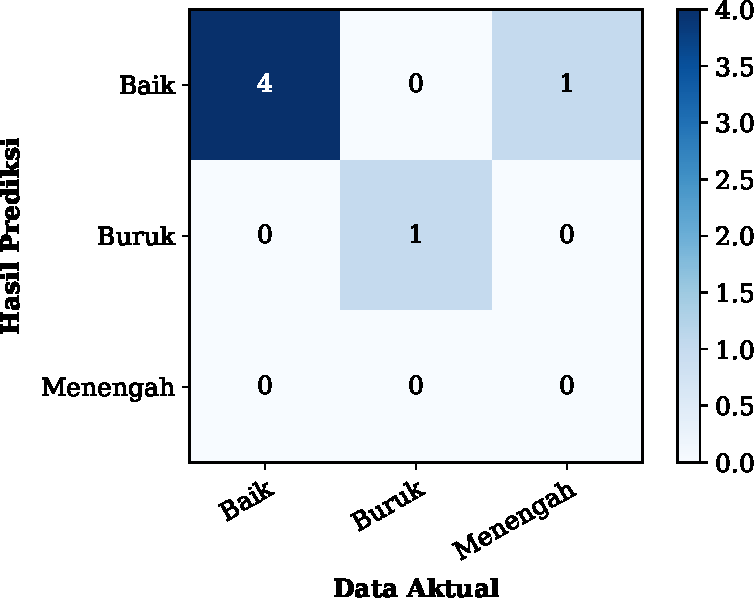
\includegraphics[width=0.6\textwidth]{BAB-4/plot/CM_rasio_data_kecil.pdf}
		\captionof{figure}{\textit{Confusion Matrix} Percobaan Menggunakan Rasio Data Pelatihan dan Pengujian 8:2}
		\label{gambar:CM rasio layer DS-2}
	\end{minipage}
}

Evaluasi untuk masing-masing kategori dapat dilihat pada Gambar \ref{gambar:presisi sensitivity rasio data kecil}. Diperoleh informasi pada gambar tersebut bahwa katergori "Menengah" mendapatkan nilai yang buruk pada presisi dan sensitivitas, sedangkan kategori "Baik" menjadi memiliki sensitivitas yang tinggi. Hal ini mengindikasikan bahwa penambahan data pada proses pelatihan semakin menguatkan pengaruh kategori "Baik" pada model dan melemahkan kategori "Menengah".

\centerline{\begin{minipage}{\linewidth}
		\centering
		\vspace{12 pt}
		%% Creator: Matplotlib, PGF backend
%%
%% To include the figure in your LaTeX document, write
%%   \input{<filename>.pgf}
%%
%% Make sure the required packages are loaded in your preamble
%%   \usepackage{pgf}
%%
%% Figures using additional raster images can only be included by \input if
%% they are in the same directory as the main LaTeX file. For loading figures
%% from other directories you can use the `import` package
%%   \usepackage{import}
%%
%% and then include the figures with
%%   \import{<path to file>}{<filename>.pgf}
%%
%% Matplotlib used the following preamble
%%
\begingroup%
\makeatletter%
\begin{pgfpicture}%
\pgfpathrectangle{\pgfpointorigin}{\pgfqpoint{5.640000in}{3.140000in}}%
\pgfusepath{use as bounding box, clip}%
\begin{pgfscope}%
\pgfsetbuttcap%
\pgfsetmiterjoin%
\pgfsetlinewidth{0.000000pt}%
\definecolor{currentstroke}{rgb}{1.000000,1.000000,1.000000}%
\pgfsetstrokecolor{currentstroke}%
\pgfsetstrokeopacity{0.000000}%
\pgfsetdash{}{0pt}%
\pgfpathmoveto{\pgfqpoint{0.000000in}{0.000000in}}%
\pgfpathlineto{\pgfqpoint{5.640000in}{0.000000in}}%
\pgfpathlineto{\pgfqpoint{5.640000in}{3.140000in}}%
\pgfpathlineto{\pgfqpoint{0.000000in}{3.140000in}}%
\pgfpathclose%
\pgfusepath{}%
\end{pgfscope}%
\begin{pgfscope}%
\pgfsetbuttcap%
\pgfsetmiterjoin%
\definecolor{currentfill}{rgb}{1.000000,1.000000,1.000000}%
\pgfsetfillcolor{currentfill}%
\pgfsetlinewidth{0.000000pt}%
\definecolor{currentstroke}{rgb}{0.000000,0.000000,0.000000}%
\pgfsetstrokecolor{currentstroke}%
\pgfsetstrokeopacity{0.000000}%
\pgfsetdash{}{0pt}%
\pgfpathmoveto{\pgfqpoint{0.453704in}{0.693723in}}%
\pgfpathlineto{\pgfqpoint{2.730000in}{0.693723in}}%
\pgfpathlineto{\pgfqpoint{2.730000in}{3.140000in}}%
\pgfpathlineto{\pgfqpoint{0.453704in}{3.140000in}}%
\pgfpathclose%
\pgfusepath{fill}%
\end{pgfscope}%
\begin{pgfscope}%
\pgfpathrectangle{\pgfqpoint{0.453704in}{0.693723in}}{\pgfqpoint{2.276296in}{2.446277in}}%
\pgfusepath{clip}%
\pgfsetbuttcap%
\pgfsetmiterjoin%
\definecolor{currentfill}{rgb}{0.121569,0.466667,0.705882}%
\pgfsetfillcolor{currentfill}%
\pgfsetlinewidth{0.000000pt}%
\definecolor{currentstroke}{rgb}{0.000000,0.000000,0.000000}%
\pgfsetstrokecolor{currentstroke}%
\pgfsetstrokeopacity{0.000000}%
\pgfsetdash{}{0pt}%
\pgfpathmoveto{\pgfqpoint{0.557172in}{0.693723in}}%
\pgfpathlineto{\pgfqpoint{0.902065in}{0.693723in}}%
\pgfpathlineto{\pgfqpoint{0.902065in}{2.177056in}}%
\pgfpathlineto{\pgfqpoint{0.557172in}{2.177056in}}%
\pgfpathclose%
\pgfusepath{fill}%
\end{pgfscope}%
\begin{pgfscope}%
\pgfpathrectangle{\pgfqpoint{0.453704in}{0.693723in}}{\pgfqpoint{2.276296in}{2.446277in}}%
\pgfusepath{clip}%
\pgfsetbuttcap%
\pgfsetmiterjoin%
\definecolor{currentfill}{rgb}{0.121569,0.466667,0.705882}%
\pgfsetfillcolor{currentfill}%
\pgfsetlinewidth{0.000000pt}%
\definecolor{currentstroke}{rgb}{0.000000,0.000000,0.000000}%
\pgfsetstrokecolor{currentstroke}%
\pgfsetstrokeopacity{0.000000}%
\pgfsetdash{}{0pt}%
\pgfpathmoveto{\pgfqpoint{1.419405in}{0.693723in}}%
\pgfpathlineto{\pgfqpoint{1.764299in}{0.693723in}}%
\pgfpathlineto{\pgfqpoint{1.764299in}{2.917611in}}%
\pgfpathlineto{\pgfqpoint{1.419405in}{2.917611in}}%
\pgfpathclose%
\pgfusepath{fill}%
\end{pgfscope}%
\begin{pgfscope}%
\pgfpathrectangle{\pgfqpoint{0.453704in}{0.693723in}}{\pgfqpoint{2.276296in}{2.446277in}}%
\pgfusepath{clip}%
\pgfsetbuttcap%
\pgfsetmiterjoin%
\definecolor{currentfill}{rgb}{0.121569,0.466667,0.705882}%
\pgfsetfillcolor{currentfill}%
\pgfsetlinewidth{0.000000pt}%
\definecolor{currentstroke}{rgb}{0.000000,0.000000,0.000000}%
\pgfsetstrokecolor{currentstroke}%
\pgfsetstrokeopacity{0.000000}%
\pgfsetdash{}{0pt}%
\pgfpathmoveto{\pgfqpoint{2.281639in}{0.693723in}}%
\pgfpathlineto{\pgfqpoint{2.626532in}{0.693723in}}%
\pgfpathlineto{\pgfqpoint{2.626532in}{0.693723in}}%
\pgfpathlineto{\pgfqpoint{2.281639in}{0.693723in}}%
\pgfpathclose%
\pgfusepath{fill}%
\end{pgfscope}%
\begin{pgfscope}%
\pgfsetbuttcap%
\pgfsetroundjoin%
\definecolor{currentfill}{rgb}{0.000000,0.000000,0.000000}%
\pgfsetfillcolor{currentfill}%
\pgfsetlinewidth{0.803000pt}%
\definecolor{currentstroke}{rgb}{0.000000,0.000000,0.000000}%
\pgfsetstrokecolor{currentstroke}%
\pgfsetdash{}{0pt}%
\pgfsys@defobject{currentmarker}{\pgfqpoint{0.000000in}{-0.048611in}}{\pgfqpoint{0.000000in}{0.000000in}}{%
\pgfpathmoveto{\pgfqpoint{0.000000in}{0.000000in}}%
\pgfpathlineto{\pgfqpoint{0.000000in}{-0.048611in}}%
\pgfusepath{stroke,fill}%
}%
\begin{pgfscope}%
\pgfsys@transformshift{0.729619in}{0.693723in}%
\pgfsys@useobject{currentmarker}{}%
\end{pgfscope}%
\end{pgfscope}%
\begin{pgfscope}%
\definecolor{textcolor}{rgb}{0.000000,0.000000,0.000000}%
\pgfsetstrokecolor{textcolor}%
\pgfsetfillcolor{textcolor}%
\pgftext[x=0.729619in,y=0.596500in,right,top,rotate=30.000000]{\color{textcolor}\rmfamily\fontsize{10.000000}{12.000000}\selectfont Baik}%
\end{pgfscope}%
\begin{pgfscope}%
\pgfsetbuttcap%
\pgfsetroundjoin%
\definecolor{currentfill}{rgb}{0.000000,0.000000,0.000000}%
\pgfsetfillcolor{currentfill}%
\pgfsetlinewidth{0.803000pt}%
\definecolor{currentstroke}{rgb}{0.000000,0.000000,0.000000}%
\pgfsetstrokecolor{currentstroke}%
\pgfsetdash{}{0pt}%
\pgfsys@defobject{currentmarker}{\pgfqpoint{0.000000in}{-0.048611in}}{\pgfqpoint{0.000000in}{0.000000in}}{%
\pgfpathmoveto{\pgfqpoint{0.000000in}{0.000000in}}%
\pgfpathlineto{\pgfqpoint{0.000000in}{-0.048611in}}%
\pgfusepath{stroke,fill}%
}%
\begin{pgfscope}%
\pgfsys@transformshift{1.591852in}{0.693723in}%
\pgfsys@useobject{currentmarker}{}%
\end{pgfscope}%
\end{pgfscope}%
\begin{pgfscope}%
\definecolor{textcolor}{rgb}{0.000000,0.000000,0.000000}%
\pgfsetstrokecolor{textcolor}%
\pgfsetfillcolor{textcolor}%
\pgftext[x=1.591852in,y=0.596500in,right,top,rotate=30.000000]{\color{textcolor}\rmfamily\fontsize{10.000000}{12.000000}\selectfont Buruk}%
\end{pgfscope}%
\begin{pgfscope}%
\pgfsetbuttcap%
\pgfsetroundjoin%
\definecolor{currentfill}{rgb}{0.000000,0.000000,0.000000}%
\pgfsetfillcolor{currentfill}%
\pgfsetlinewidth{0.803000pt}%
\definecolor{currentstroke}{rgb}{0.000000,0.000000,0.000000}%
\pgfsetstrokecolor{currentstroke}%
\pgfsetdash{}{0pt}%
\pgfsys@defobject{currentmarker}{\pgfqpoint{0.000000in}{-0.048611in}}{\pgfqpoint{0.000000in}{0.000000in}}{%
\pgfpathmoveto{\pgfqpoint{0.000000in}{0.000000in}}%
\pgfpathlineto{\pgfqpoint{0.000000in}{-0.048611in}}%
\pgfusepath{stroke,fill}%
}%
\begin{pgfscope}%
\pgfsys@transformshift{2.454085in}{0.693723in}%
\pgfsys@useobject{currentmarker}{}%
\end{pgfscope}%
\end{pgfscope}%
\begin{pgfscope}%
\definecolor{textcolor}{rgb}{0.000000,0.000000,0.000000}%
\pgfsetstrokecolor{textcolor}%
\pgfsetfillcolor{textcolor}%
\pgftext[x=2.454085in,y=0.596500in,right,top,rotate=30.000000]{\color{textcolor}\rmfamily\fontsize{10.000000}{12.000000}\selectfont Menengah}%
\end{pgfscope}%
\begin{pgfscope}%
\definecolor{textcolor}{rgb}{0.000000,0.000000,0.000000}%
\pgfsetstrokecolor{textcolor}%
\pgfsetfillcolor{textcolor}%
\pgftext[x=1.591852in,y=0.123457in,,top]{\color{textcolor}\rmfamily\fontsize{10.000000}{12.000000}\selectfont Kategori}%
\end{pgfscope}%
\begin{pgfscope}%
\pgfsetbuttcap%
\pgfsetroundjoin%
\definecolor{currentfill}{rgb}{0.000000,0.000000,0.000000}%
\pgfsetfillcolor{currentfill}%
\pgfsetlinewidth{0.803000pt}%
\definecolor{currentstroke}{rgb}{0.000000,0.000000,0.000000}%
\pgfsetstrokecolor{currentstroke}%
\pgfsetdash{}{0pt}%
\pgfsys@defobject{currentmarker}{\pgfqpoint{-0.048611in}{0.000000in}}{\pgfqpoint{-0.000000in}{0.000000in}}{%
\pgfpathmoveto{\pgfqpoint{-0.000000in}{0.000000in}}%
\pgfpathlineto{\pgfqpoint{-0.048611in}{0.000000in}}%
\pgfusepath{stroke,fill}%
}%
\begin{pgfscope}%
\pgfsys@transformshift{0.453704in}{0.693723in}%
\pgfsys@useobject{currentmarker}{}%
\end{pgfscope}%
\end{pgfscope}%
\begin{pgfscope}%
\definecolor{textcolor}{rgb}{0.000000,0.000000,0.000000}%
\pgfsetstrokecolor{textcolor}%
\pgfsetfillcolor{textcolor}%
\pgftext[x=0.179012in, y=0.645497in, left, base]{\color{textcolor}\rmfamily\fontsize{10.000000}{12.000000}\selectfont \(\displaystyle {0.0}\)}%
\end{pgfscope}%
\begin{pgfscope}%
\pgfsetbuttcap%
\pgfsetroundjoin%
\definecolor{currentfill}{rgb}{0.000000,0.000000,0.000000}%
\pgfsetfillcolor{currentfill}%
\pgfsetlinewidth{0.803000pt}%
\definecolor{currentstroke}{rgb}{0.000000,0.000000,0.000000}%
\pgfsetstrokecolor{currentstroke}%
\pgfsetdash{}{0pt}%
\pgfsys@defobject{currentmarker}{\pgfqpoint{-0.048611in}{0.000000in}}{\pgfqpoint{-0.000000in}{0.000000in}}{%
\pgfpathmoveto{\pgfqpoint{-0.000000in}{0.000000in}}%
\pgfpathlineto{\pgfqpoint{-0.048611in}{0.000000in}}%
\pgfusepath{stroke,fill}%
}%
\begin{pgfscope}%
\pgfsys@transformshift{0.453704in}{1.138500in}%
\pgfsys@useobject{currentmarker}{}%
\end{pgfscope}%
\end{pgfscope}%
\begin{pgfscope}%
\definecolor{textcolor}{rgb}{0.000000,0.000000,0.000000}%
\pgfsetstrokecolor{textcolor}%
\pgfsetfillcolor{textcolor}%
\pgftext[x=0.179012in, y=1.090275in, left, base]{\color{textcolor}\rmfamily\fontsize{10.000000}{12.000000}\selectfont \(\displaystyle {0.2}\)}%
\end{pgfscope}%
\begin{pgfscope}%
\pgfsetbuttcap%
\pgfsetroundjoin%
\definecolor{currentfill}{rgb}{0.000000,0.000000,0.000000}%
\pgfsetfillcolor{currentfill}%
\pgfsetlinewidth{0.803000pt}%
\definecolor{currentstroke}{rgb}{0.000000,0.000000,0.000000}%
\pgfsetstrokecolor{currentstroke}%
\pgfsetdash{}{0pt}%
\pgfsys@defobject{currentmarker}{\pgfqpoint{-0.048611in}{0.000000in}}{\pgfqpoint{-0.000000in}{0.000000in}}{%
\pgfpathmoveto{\pgfqpoint{-0.000000in}{0.000000in}}%
\pgfpathlineto{\pgfqpoint{-0.048611in}{0.000000in}}%
\pgfusepath{stroke,fill}%
}%
\begin{pgfscope}%
\pgfsys@transformshift{0.453704in}{1.583278in}%
\pgfsys@useobject{currentmarker}{}%
\end{pgfscope}%
\end{pgfscope}%
\begin{pgfscope}%
\definecolor{textcolor}{rgb}{0.000000,0.000000,0.000000}%
\pgfsetstrokecolor{textcolor}%
\pgfsetfillcolor{textcolor}%
\pgftext[x=0.179012in, y=1.535053in, left, base]{\color{textcolor}\rmfamily\fontsize{10.000000}{12.000000}\selectfont \(\displaystyle {0.4}\)}%
\end{pgfscope}%
\begin{pgfscope}%
\pgfsetbuttcap%
\pgfsetroundjoin%
\definecolor{currentfill}{rgb}{0.000000,0.000000,0.000000}%
\pgfsetfillcolor{currentfill}%
\pgfsetlinewidth{0.803000pt}%
\definecolor{currentstroke}{rgb}{0.000000,0.000000,0.000000}%
\pgfsetstrokecolor{currentstroke}%
\pgfsetdash{}{0pt}%
\pgfsys@defobject{currentmarker}{\pgfqpoint{-0.048611in}{0.000000in}}{\pgfqpoint{-0.000000in}{0.000000in}}{%
\pgfpathmoveto{\pgfqpoint{-0.000000in}{0.000000in}}%
\pgfpathlineto{\pgfqpoint{-0.048611in}{0.000000in}}%
\pgfusepath{stroke,fill}%
}%
\begin{pgfscope}%
\pgfsys@transformshift{0.453704in}{2.028056in}%
\pgfsys@useobject{currentmarker}{}%
\end{pgfscope}%
\end{pgfscope}%
\begin{pgfscope}%
\definecolor{textcolor}{rgb}{0.000000,0.000000,0.000000}%
\pgfsetstrokecolor{textcolor}%
\pgfsetfillcolor{textcolor}%
\pgftext[x=0.179012in, y=1.979831in, left, base]{\color{textcolor}\rmfamily\fontsize{10.000000}{12.000000}\selectfont \(\displaystyle {0.6}\)}%
\end{pgfscope}%
\begin{pgfscope}%
\pgfsetbuttcap%
\pgfsetroundjoin%
\definecolor{currentfill}{rgb}{0.000000,0.000000,0.000000}%
\pgfsetfillcolor{currentfill}%
\pgfsetlinewidth{0.803000pt}%
\definecolor{currentstroke}{rgb}{0.000000,0.000000,0.000000}%
\pgfsetstrokecolor{currentstroke}%
\pgfsetdash{}{0pt}%
\pgfsys@defobject{currentmarker}{\pgfqpoint{-0.048611in}{0.000000in}}{\pgfqpoint{-0.000000in}{0.000000in}}{%
\pgfpathmoveto{\pgfqpoint{-0.000000in}{0.000000in}}%
\pgfpathlineto{\pgfqpoint{-0.048611in}{0.000000in}}%
\pgfusepath{stroke,fill}%
}%
\begin{pgfscope}%
\pgfsys@transformshift{0.453704in}{2.472833in}%
\pgfsys@useobject{currentmarker}{}%
\end{pgfscope}%
\end{pgfscope}%
\begin{pgfscope}%
\definecolor{textcolor}{rgb}{0.000000,0.000000,0.000000}%
\pgfsetstrokecolor{textcolor}%
\pgfsetfillcolor{textcolor}%
\pgftext[x=0.179012in, y=2.424608in, left, base]{\color{textcolor}\rmfamily\fontsize{10.000000}{12.000000}\selectfont \(\displaystyle {0.8}\)}%
\end{pgfscope}%
\begin{pgfscope}%
\pgfsetbuttcap%
\pgfsetroundjoin%
\definecolor{currentfill}{rgb}{0.000000,0.000000,0.000000}%
\pgfsetfillcolor{currentfill}%
\pgfsetlinewidth{0.803000pt}%
\definecolor{currentstroke}{rgb}{0.000000,0.000000,0.000000}%
\pgfsetstrokecolor{currentstroke}%
\pgfsetdash{}{0pt}%
\pgfsys@defobject{currentmarker}{\pgfqpoint{-0.048611in}{0.000000in}}{\pgfqpoint{-0.000000in}{0.000000in}}{%
\pgfpathmoveto{\pgfqpoint{-0.000000in}{0.000000in}}%
\pgfpathlineto{\pgfqpoint{-0.048611in}{0.000000in}}%
\pgfusepath{stroke,fill}%
}%
\begin{pgfscope}%
\pgfsys@transformshift{0.453704in}{2.917611in}%
\pgfsys@useobject{currentmarker}{}%
\end{pgfscope}%
\end{pgfscope}%
\begin{pgfscope}%
\definecolor{textcolor}{rgb}{0.000000,0.000000,0.000000}%
\pgfsetstrokecolor{textcolor}%
\pgfsetfillcolor{textcolor}%
\pgftext[x=0.179012in, y=2.869386in, left, base]{\color{textcolor}\rmfamily\fontsize{10.000000}{12.000000}\selectfont \(\displaystyle {1.0}\)}%
\end{pgfscope}%
\begin{pgfscope}%
\definecolor{textcolor}{rgb}{0.000000,0.000000,0.000000}%
\pgfsetstrokecolor{textcolor}%
\pgfsetfillcolor{textcolor}%
\pgftext[x=0.123457in,y=1.916861in,,bottom,rotate=90.000000]{\color{textcolor}\rmfamily\fontsize{10.000000}{12.000000}\selectfont Presisi}%
\end{pgfscope}%
\begin{pgfscope}%
\pgfsetrectcap%
\pgfsetmiterjoin%
\pgfsetlinewidth{0.803000pt}%
\definecolor{currentstroke}{rgb}{0.000000,0.000000,0.000000}%
\pgfsetstrokecolor{currentstroke}%
\pgfsetdash{}{0pt}%
\pgfpathmoveto{\pgfqpoint{0.453704in}{0.693723in}}%
\pgfpathlineto{\pgfqpoint{0.453704in}{3.140000in}}%
\pgfusepath{stroke}%
\end{pgfscope}%
\begin{pgfscope}%
\pgfsetrectcap%
\pgfsetmiterjoin%
\pgfsetlinewidth{0.803000pt}%
\definecolor{currentstroke}{rgb}{0.000000,0.000000,0.000000}%
\pgfsetstrokecolor{currentstroke}%
\pgfsetdash{}{0pt}%
\pgfpathmoveto{\pgfqpoint{2.730000in}{0.693723in}}%
\pgfpathlineto{\pgfqpoint{2.730000in}{3.140000in}}%
\pgfusepath{stroke}%
\end{pgfscope}%
\begin{pgfscope}%
\pgfsetrectcap%
\pgfsetmiterjoin%
\pgfsetlinewidth{0.803000pt}%
\definecolor{currentstroke}{rgb}{0.000000,0.000000,0.000000}%
\pgfsetstrokecolor{currentstroke}%
\pgfsetdash{}{0pt}%
\pgfpathmoveto{\pgfqpoint{0.453704in}{0.693723in}}%
\pgfpathlineto{\pgfqpoint{2.730000in}{0.693723in}}%
\pgfusepath{stroke}%
\end{pgfscope}%
\begin{pgfscope}%
\pgfsetrectcap%
\pgfsetmiterjoin%
\pgfsetlinewidth{0.803000pt}%
\definecolor{currentstroke}{rgb}{0.000000,0.000000,0.000000}%
\pgfsetstrokecolor{currentstroke}%
\pgfsetdash{}{0pt}%
\pgfpathmoveto{\pgfqpoint{0.453704in}{3.140000in}}%
\pgfpathlineto{\pgfqpoint{2.730000in}{3.140000in}}%
\pgfusepath{stroke}%
\end{pgfscope}%
\begin{pgfscope}%
\definecolor{textcolor}{rgb}{0.000000,0.000000,0.000000}%
\pgfsetstrokecolor{textcolor}%
\pgfsetfillcolor{textcolor}%
\pgftext[x=0.729619in,y=2.199295in,,bottom]{\color{textcolor}\rmfamily\fontsize{9.000000}{10.800000}\selectfont 0.667}%
\end{pgfscope}%
\begin{pgfscope}%
\definecolor{textcolor}{rgb}{0.000000,0.000000,0.000000}%
\pgfsetstrokecolor{textcolor}%
\pgfsetfillcolor{textcolor}%
\pgftext[x=1.591852in,y=2.939850in,,bottom]{\color{textcolor}\rmfamily\fontsize{9.000000}{10.800000}\selectfont 1.0}%
\end{pgfscope}%
\begin{pgfscope}%
\definecolor{textcolor}{rgb}{0.000000,0.000000,0.000000}%
\pgfsetstrokecolor{textcolor}%
\pgfsetfillcolor{textcolor}%
\pgftext[x=2.454085in,y=0.715962in,,bottom]{\color{textcolor}\rmfamily\fontsize{9.000000}{10.800000}\selectfont 0.0}%
\end{pgfscope}%
\begin{pgfscope}%
\pgfsetbuttcap%
\pgfsetmiterjoin%
\definecolor{currentfill}{rgb}{1.000000,1.000000,1.000000}%
\pgfsetfillcolor{currentfill}%
\pgfsetlinewidth{0.000000pt}%
\definecolor{currentstroke}{rgb}{0.000000,0.000000,0.000000}%
\pgfsetstrokecolor{currentstroke}%
\pgfsetstrokeopacity{0.000000}%
\pgfsetdash{}{0pt}%
\pgfpathmoveto{\pgfqpoint{3.363704in}{0.693723in}}%
\pgfpathlineto{\pgfqpoint{5.640000in}{0.693723in}}%
\pgfpathlineto{\pgfqpoint{5.640000in}{3.140000in}}%
\pgfpathlineto{\pgfqpoint{3.363704in}{3.140000in}}%
\pgfpathclose%
\pgfusepath{fill}%
\end{pgfscope}%
\begin{pgfscope}%
\pgfpathrectangle{\pgfqpoint{3.363704in}{0.693723in}}{\pgfqpoint{2.276296in}{2.446277in}}%
\pgfusepath{clip}%
\pgfsetbuttcap%
\pgfsetmiterjoin%
\definecolor{currentfill}{rgb}{1.000000,0.498039,0.054902}%
\pgfsetfillcolor{currentfill}%
\pgfsetlinewidth{0.000000pt}%
\definecolor{currentstroke}{rgb}{0.000000,0.000000,0.000000}%
\pgfsetstrokecolor{currentstroke}%
\pgfsetstrokeopacity{0.000000}%
\pgfsetdash{}{0pt}%
\pgfpathmoveto{\pgfqpoint{3.467172in}{0.693723in}}%
\pgfpathlineto{\pgfqpoint{3.812065in}{0.693723in}}%
\pgfpathlineto{\pgfqpoint{3.812065in}{2.917611in}}%
\pgfpathlineto{\pgfqpoint{3.467172in}{2.917611in}}%
\pgfpathclose%
\pgfusepath{fill}%
\end{pgfscope}%
\begin{pgfscope}%
\pgfpathrectangle{\pgfqpoint{3.363704in}{0.693723in}}{\pgfqpoint{2.276296in}{2.446277in}}%
\pgfusepath{clip}%
\pgfsetbuttcap%
\pgfsetmiterjoin%
\definecolor{currentfill}{rgb}{1.000000,0.498039,0.054902}%
\pgfsetfillcolor{currentfill}%
\pgfsetlinewidth{0.000000pt}%
\definecolor{currentstroke}{rgb}{0.000000,0.000000,0.000000}%
\pgfsetstrokecolor{currentstroke}%
\pgfsetstrokeopacity{0.000000}%
\pgfsetdash{}{0pt}%
\pgfpathmoveto{\pgfqpoint{4.329405in}{0.693723in}}%
\pgfpathlineto{\pgfqpoint{4.674299in}{0.693723in}}%
\pgfpathlineto{\pgfqpoint{4.674299in}{2.361639in}}%
\pgfpathlineto{\pgfqpoint{4.329405in}{2.361639in}}%
\pgfpathclose%
\pgfusepath{fill}%
\end{pgfscope}%
\begin{pgfscope}%
\pgfpathrectangle{\pgfqpoint{3.363704in}{0.693723in}}{\pgfqpoint{2.276296in}{2.446277in}}%
\pgfusepath{clip}%
\pgfsetbuttcap%
\pgfsetmiterjoin%
\definecolor{currentfill}{rgb}{1.000000,0.498039,0.054902}%
\pgfsetfillcolor{currentfill}%
\pgfsetlinewidth{0.000000pt}%
\definecolor{currentstroke}{rgb}{0.000000,0.000000,0.000000}%
\pgfsetstrokecolor{currentstroke}%
\pgfsetstrokeopacity{0.000000}%
\pgfsetdash{}{0pt}%
\pgfpathmoveto{\pgfqpoint{5.191639in}{0.693723in}}%
\pgfpathlineto{\pgfqpoint{5.536532in}{0.693723in}}%
\pgfpathlineto{\pgfqpoint{5.536532in}{0.693723in}}%
\pgfpathlineto{\pgfqpoint{5.191639in}{0.693723in}}%
\pgfpathclose%
\pgfusepath{fill}%
\end{pgfscope}%
\begin{pgfscope}%
\pgfsetbuttcap%
\pgfsetroundjoin%
\definecolor{currentfill}{rgb}{0.000000,0.000000,0.000000}%
\pgfsetfillcolor{currentfill}%
\pgfsetlinewidth{0.803000pt}%
\definecolor{currentstroke}{rgb}{0.000000,0.000000,0.000000}%
\pgfsetstrokecolor{currentstroke}%
\pgfsetdash{}{0pt}%
\pgfsys@defobject{currentmarker}{\pgfqpoint{0.000000in}{-0.048611in}}{\pgfqpoint{0.000000in}{0.000000in}}{%
\pgfpathmoveto{\pgfqpoint{0.000000in}{0.000000in}}%
\pgfpathlineto{\pgfqpoint{0.000000in}{-0.048611in}}%
\pgfusepath{stroke,fill}%
}%
\begin{pgfscope}%
\pgfsys@transformshift{3.639619in}{0.693723in}%
\pgfsys@useobject{currentmarker}{}%
\end{pgfscope}%
\end{pgfscope}%
\begin{pgfscope}%
\definecolor{textcolor}{rgb}{0.000000,0.000000,0.000000}%
\pgfsetstrokecolor{textcolor}%
\pgfsetfillcolor{textcolor}%
\pgftext[x=3.639619in,y=0.596500in,right,top,rotate=30.000000]{\color{textcolor}\rmfamily\fontsize{10.000000}{12.000000}\selectfont Baik}%
\end{pgfscope}%
\begin{pgfscope}%
\pgfsetbuttcap%
\pgfsetroundjoin%
\definecolor{currentfill}{rgb}{0.000000,0.000000,0.000000}%
\pgfsetfillcolor{currentfill}%
\pgfsetlinewidth{0.803000pt}%
\definecolor{currentstroke}{rgb}{0.000000,0.000000,0.000000}%
\pgfsetstrokecolor{currentstroke}%
\pgfsetdash{}{0pt}%
\pgfsys@defobject{currentmarker}{\pgfqpoint{0.000000in}{-0.048611in}}{\pgfqpoint{0.000000in}{0.000000in}}{%
\pgfpathmoveto{\pgfqpoint{0.000000in}{0.000000in}}%
\pgfpathlineto{\pgfqpoint{0.000000in}{-0.048611in}}%
\pgfusepath{stroke,fill}%
}%
\begin{pgfscope}%
\pgfsys@transformshift{4.501852in}{0.693723in}%
\pgfsys@useobject{currentmarker}{}%
\end{pgfscope}%
\end{pgfscope}%
\begin{pgfscope}%
\definecolor{textcolor}{rgb}{0.000000,0.000000,0.000000}%
\pgfsetstrokecolor{textcolor}%
\pgfsetfillcolor{textcolor}%
\pgftext[x=4.501852in,y=0.596500in,right,top,rotate=30.000000]{\color{textcolor}\rmfamily\fontsize{10.000000}{12.000000}\selectfont Buruk}%
\end{pgfscope}%
\begin{pgfscope}%
\pgfsetbuttcap%
\pgfsetroundjoin%
\definecolor{currentfill}{rgb}{0.000000,0.000000,0.000000}%
\pgfsetfillcolor{currentfill}%
\pgfsetlinewidth{0.803000pt}%
\definecolor{currentstroke}{rgb}{0.000000,0.000000,0.000000}%
\pgfsetstrokecolor{currentstroke}%
\pgfsetdash{}{0pt}%
\pgfsys@defobject{currentmarker}{\pgfqpoint{0.000000in}{-0.048611in}}{\pgfqpoint{0.000000in}{0.000000in}}{%
\pgfpathmoveto{\pgfqpoint{0.000000in}{0.000000in}}%
\pgfpathlineto{\pgfqpoint{0.000000in}{-0.048611in}}%
\pgfusepath{stroke,fill}%
}%
\begin{pgfscope}%
\pgfsys@transformshift{5.364085in}{0.693723in}%
\pgfsys@useobject{currentmarker}{}%
\end{pgfscope}%
\end{pgfscope}%
\begin{pgfscope}%
\definecolor{textcolor}{rgb}{0.000000,0.000000,0.000000}%
\pgfsetstrokecolor{textcolor}%
\pgfsetfillcolor{textcolor}%
\pgftext[x=5.364085in,y=0.596500in,right,top,rotate=30.000000]{\color{textcolor}\rmfamily\fontsize{10.000000}{12.000000}\selectfont Menengah}%
\end{pgfscope}%
\begin{pgfscope}%
\definecolor{textcolor}{rgb}{0.000000,0.000000,0.000000}%
\pgfsetstrokecolor{textcolor}%
\pgfsetfillcolor{textcolor}%
\pgftext[x=4.501852in,y=0.123457in,,top]{\color{textcolor}\rmfamily\fontsize{10.000000}{12.000000}\selectfont Kategori}%
\end{pgfscope}%
\begin{pgfscope}%
\pgfsetbuttcap%
\pgfsetroundjoin%
\definecolor{currentfill}{rgb}{0.000000,0.000000,0.000000}%
\pgfsetfillcolor{currentfill}%
\pgfsetlinewidth{0.803000pt}%
\definecolor{currentstroke}{rgb}{0.000000,0.000000,0.000000}%
\pgfsetstrokecolor{currentstroke}%
\pgfsetdash{}{0pt}%
\pgfsys@defobject{currentmarker}{\pgfqpoint{-0.048611in}{0.000000in}}{\pgfqpoint{-0.000000in}{0.000000in}}{%
\pgfpathmoveto{\pgfqpoint{-0.000000in}{0.000000in}}%
\pgfpathlineto{\pgfqpoint{-0.048611in}{0.000000in}}%
\pgfusepath{stroke,fill}%
}%
\begin{pgfscope}%
\pgfsys@transformshift{3.363704in}{0.693723in}%
\pgfsys@useobject{currentmarker}{}%
\end{pgfscope}%
\end{pgfscope}%
\begin{pgfscope}%
\definecolor{textcolor}{rgb}{0.000000,0.000000,0.000000}%
\pgfsetstrokecolor{textcolor}%
\pgfsetfillcolor{textcolor}%
\pgftext[x=3.089012in, y=0.645497in, left, base]{\color{textcolor}\rmfamily\fontsize{10.000000}{12.000000}\selectfont \(\displaystyle {0.0}\)}%
\end{pgfscope}%
\begin{pgfscope}%
\pgfsetbuttcap%
\pgfsetroundjoin%
\definecolor{currentfill}{rgb}{0.000000,0.000000,0.000000}%
\pgfsetfillcolor{currentfill}%
\pgfsetlinewidth{0.803000pt}%
\definecolor{currentstroke}{rgb}{0.000000,0.000000,0.000000}%
\pgfsetstrokecolor{currentstroke}%
\pgfsetdash{}{0pt}%
\pgfsys@defobject{currentmarker}{\pgfqpoint{-0.048611in}{0.000000in}}{\pgfqpoint{-0.000000in}{0.000000in}}{%
\pgfpathmoveto{\pgfqpoint{-0.000000in}{0.000000in}}%
\pgfpathlineto{\pgfqpoint{-0.048611in}{0.000000in}}%
\pgfusepath{stroke,fill}%
}%
\begin{pgfscope}%
\pgfsys@transformshift{3.363704in}{1.138500in}%
\pgfsys@useobject{currentmarker}{}%
\end{pgfscope}%
\end{pgfscope}%
\begin{pgfscope}%
\definecolor{textcolor}{rgb}{0.000000,0.000000,0.000000}%
\pgfsetstrokecolor{textcolor}%
\pgfsetfillcolor{textcolor}%
\pgftext[x=3.089012in, y=1.090275in, left, base]{\color{textcolor}\rmfamily\fontsize{10.000000}{12.000000}\selectfont \(\displaystyle {0.2}\)}%
\end{pgfscope}%
\begin{pgfscope}%
\pgfsetbuttcap%
\pgfsetroundjoin%
\definecolor{currentfill}{rgb}{0.000000,0.000000,0.000000}%
\pgfsetfillcolor{currentfill}%
\pgfsetlinewidth{0.803000pt}%
\definecolor{currentstroke}{rgb}{0.000000,0.000000,0.000000}%
\pgfsetstrokecolor{currentstroke}%
\pgfsetdash{}{0pt}%
\pgfsys@defobject{currentmarker}{\pgfqpoint{-0.048611in}{0.000000in}}{\pgfqpoint{-0.000000in}{0.000000in}}{%
\pgfpathmoveto{\pgfqpoint{-0.000000in}{0.000000in}}%
\pgfpathlineto{\pgfqpoint{-0.048611in}{0.000000in}}%
\pgfusepath{stroke,fill}%
}%
\begin{pgfscope}%
\pgfsys@transformshift{3.363704in}{1.583278in}%
\pgfsys@useobject{currentmarker}{}%
\end{pgfscope}%
\end{pgfscope}%
\begin{pgfscope}%
\definecolor{textcolor}{rgb}{0.000000,0.000000,0.000000}%
\pgfsetstrokecolor{textcolor}%
\pgfsetfillcolor{textcolor}%
\pgftext[x=3.089012in, y=1.535053in, left, base]{\color{textcolor}\rmfamily\fontsize{10.000000}{12.000000}\selectfont \(\displaystyle {0.4}\)}%
\end{pgfscope}%
\begin{pgfscope}%
\pgfsetbuttcap%
\pgfsetroundjoin%
\definecolor{currentfill}{rgb}{0.000000,0.000000,0.000000}%
\pgfsetfillcolor{currentfill}%
\pgfsetlinewidth{0.803000pt}%
\definecolor{currentstroke}{rgb}{0.000000,0.000000,0.000000}%
\pgfsetstrokecolor{currentstroke}%
\pgfsetdash{}{0pt}%
\pgfsys@defobject{currentmarker}{\pgfqpoint{-0.048611in}{0.000000in}}{\pgfqpoint{-0.000000in}{0.000000in}}{%
\pgfpathmoveto{\pgfqpoint{-0.000000in}{0.000000in}}%
\pgfpathlineto{\pgfqpoint{-0.048611in}{0.000000in}}%
\pgfusepath{stroke,fill}%
}%
\begin{pgfscope}%
\pgfsys@transformshift{3.363704in}{2.028056in}%
\pgfsys@useobject{currentmarker}{}%
\end{pgfscope}%
\end{pgfscope}%
\begin{pgfscope}%
\definecolor{textcolor}{rgb}{0.000000,0.000000,0.000000}%
\pgfsetstrokecolor{textcolor}%
\pgfsetfillcolor{textcolor}%
\pgftext[x=3.089012in, y=1.979831in, left, base]{\color{textcolor}\rmfamily\fontsize{10.000000}{12.000000}\selectfont \(\displaystyle {0.6}\)}%
\end{pgfscope}%
\begin{pgfscope}%
\pgfsetbuttcap%
\pgfsetroundjoin%
\definecolor{currentfill}{rgb}{0.000000,0.000000,0.000000}%
\pgfsetfillcolor{currentfill}%
\pgfsetlinewidth{0.803000pt}%
\definecolor{currentstroke}{rgb}{0.000000,0.000000,0.000000}%
\pgfsetstrokecolor{currentstroke}%
\pgfsetdash{}{0pt}%
\pgfsys@defobject{currentmarker}{\pgfqpoint{-0.048611in}{0.000000in}}{\pgfqpoint{-0.000000in}{0.000000in}}{%
\pgfpathmoveto{\pgfqpoint{-0.000000in}{0.000000in}}%
\pgfpathlineto{\pgfqpoint{-0.048611in}{0.000000in}}%
\pgfusepath{stroke,fill}%
}%
\begin{pgfscope}%
\pgfsys@transformshift{3.363704in}{2.472833in}%
\pgfsys@useobject{currentmarker}{}%
\end{pgfscope}%
\end{pgfscope}%
\begin{pgfscope}%
\definecolor{textcolor}{rgb}{0.000000,0.000000,0.000000}%
\pgfsetstrokecolor{textcolor}%
\pgfsetfillcolor{textcolor}%
\pgftext[x=3.089012in, y=2.424608in, left, base]{\color{textcolor}\rmfamily\fontsize{10.000000}{12.000000}\selectfont \(\displaystyle {0.8}\)}%
\end{pgfscope}%
\begin{pgfscope}%
\pgfsetbuttcap%
\pgfsetroundjoin%
\definecolor{currentfill}{rgb}{0.000000,0.000000,0.000000}%
\pgfsetfillcolor{currentfill}%
\pgfsetlinewidth{0.803000pt}%
\definecolor{currentstroke}{rgb}{0.000000,0.000000,0.000000}%
\pgfsetstrokecolor{currentstroke}%
\pgfsetdash{}{0pt}%
\pgfsys@defobject{currentmarker}{\pgfqpoint{-0.048611in}{0.000000in}}{\pgfqpoint{-0.000000in}{0.000000in}}{%
\pgfpathmoveto{\pgfqpoint{-0.000000in}{0.000000in}}%
\pgfpathlineto{\pgfqpoint{-0.048611in}{0.000000in}}%
\pgfusepath{stroke,fill}%
}%
\begin{pgfscope}%
\pgfsys@transformshift{3.363704in}{2.917611in}%
\pgfsys@useobject{currentmarker}{}%
\end{pgfscope}%
\end{pgfscope}%
\begin{pgfscope}%
\definecolor{textcolor}{rgb}{0.000000,0.000000,0.000000}%
\pgfsetstrokecolor{textcolor}%
\pgfsetfillcolor{textcolor}%
\pgftext[x=3.089012in, y=2.869386in, left, base]{\color{textcolor}\rmfamily\fontsize{10.000000}{12.000000}\selectfont \(\displaystyle {1.0}\)}%
\end{pgfscope}%
\begin{pgfscope}%
\definecolor{textcolor}{rgb}{0.000000,0.000000,0.000000}%
\pgfsetstrokecolor{textcolor}%
\pgfsetfillcolor{textcolor}%
\pgftext[x=3.033457in,y=1.916861in,,bottom,rotate=90.000000]{\color{textcolor}\rmfamily\fontsize{10.000000}{12.000000}\selectfont Sensitivity}%
\end{pgfscope}%
\begin{pgfscope}%
\pgfsetrectcap%
\pgfsetmiterjoin%
\pgfsetlinewidth{0.803000pt}%
\definecolor{currentstroke}{rgb}{0.000000,0.000000,0.000000}%
\pgfsetstrokecolor{currentstroke}%
\pgfsetdash{}{0pt}%
\pgfpathmoveto{\pgfqpoint{3.363704in}{0.693723in}}%
\pgfpathlineto{\pgfqpoint{3.363704in}{3.140000in}}%
\pgfusepath{stroke}%
\end{pgfscope}%
\begin{pgfscope}%
\pgfsetrectcap%
\pgfsetmiterjoin%
\pgfsetlinewidth{0.803000pt}%
\definecolor{currentstroke}{rgb}{0.000000,0.000000,0.000000}%
\pgfsetstrokecolor{currentstroke}%
\pgfsetdash{}{0pt}%
\pgfpathmoveto{\pgfqpoint{5.640000in}{0.693723in}}%
\pgfpathlineto{\pgfqpoint{5.640000in}{3.140000in}}%
\pgfusepath{stroke}%
\end{pgfscope}%
\begin{pgfscope}%
\pgfsetrectcap%
\pgfsetmiterjoin%
\pgfsetlinewidth{0.803000pt}%
\definecolor{currentstroke}{rgb}{0.000000,0.000000,0.000000}%
\pgfsetstrokecolor{currentstroke}%
\pgfsetdash{}{0pt}%
\pgfpathmoveto{\pgfqpoint{3.363704in}{0.693723in}}%
\pgfpathlineto{\pgfqpoint{5.640000in}{0.693723in}}%
\pgfusepath{stroke}%
\end{pgfscope}%
\begin{pgfscope}%
\pgfsetrectcap%
\pgfsetmiterjoin%
\pgfsetlinewidth{0.803000pt}%
\definecolor{currentstroke}{rgb}{0.000000,0.000000,0.000000}%
\pgfsetstrokecolor{currentstroke}%
\pgfsetdash{}{0pt}%
\pgfpathmoveto{\pgfqpoint{3.363704in}{3.140000in}}%
\pgfpathlineto{\pgfqpoint{5.640000in}{3.140000in}}%
\pgfusepath{stroke}%
\end{pgfscope}%
\begin{pgfscope}%
\definecolor{textcolor}{rgb}{0.000000,0.000000,0.000000}%
\pgfsetstrokecolor{textcolor}%
\pgfsetfillcolor{textcolor}%
\pgftext[x=3.639619in,y=2.939850in,,bottom]{\color{textcolor}\rmfamily\fontsize{9.000000}{10.800000}\selectfont 1.0}%
\end{pgfscope}%
\begin{pgfscope}%
\definecolor{textcolor}{rgb}{0.000000,0.000000,0.000000}%
\pgfsetstrokecolor{textcolor}%
\pgfsetfillcolor{textcolor}%
\pgftext[x=4.501852in,y=2.383878in,,bottom]{\color{textcolor}\rmfamily\fontsize{9.000000}{10.800000}\selectfont 0.75}%
\end{pgfscope}%
\begin{pgfscope}%
\definecolor{textcolor}{rgb}{0.000000,0.000000,0.000000}%
\pgfsetstrokecolor{textcolor}%
\pgfsetfillcolor{textcolor}%
\pgftext[x=5.364085in,y=0.715962in,,bottom]{\color{textcolor}\rmfamily\fontsize{9.000000}{10.800000}\selectfont 0.0}%
\end{pgfscope}%
\end{pgfpicture}%
\makeatother%
\endgroup%

		\captionof{figure}{Grafik Presisi dan Sensitivitas Menggunakan Rasio Data Pelatihan dan Pengujian 8:2}
		\label{gambar:presisi sensitivity rasio data kecil}
\end{minipage}}

Dengan demikian implementasi model pada aplikasi yang akan dipilih adalah model pada percobaan sebelumnya, yakni percobaan dengan menggunakan rasio data 7:3 dengan jumlah \textit{hidden layer} tunggal serta fungsi aktivasi "\textit{selu}.

\section{Perbandingan Terhadap Metode \textit{Artificial Neural Network} (ANN) Sederhana}
Dalam mempertimbangkan penggunaan LSTM sebagai metode utama untuk mendiagnosis indeks kesehatan transformator daya, maka dilakukan juga percobaan perbandingan terhadap metode dasar dengan menggunakan arsitektur dari ANN. Pada percobaan ini dilakukan dengan menggunakan set data 2. Pertimbangan ini diambil karena pada percobaan dengan menggunakan model LSTM jika dibandingkan, pada studi kasus 2 yang menggunakan set data 2 lebih cenderung mendapatkan performa yang rendah. Oleh karena itu percobaan ini akan membuktikan pertimbangan penggunaan LSTM sebagai pengganti dari ANN. 
Pada percobaan dilakukan dengan sebanyak 30 iterasi kemudian diambil nilai rata-rata akurasi baik pada pelatihan maupun pada pengujian. Set data yang digunakan dibagi atas data pelatihan dan pengujian dengan rasio 7:3. \textit{Hyperparameter} uji yang digunakan adalah jumlah dari \textit{hidden neuron} yang setiap percobaan berjumlah 5, 8, 11, 13, 15, 20, 25, dan 30. 

\centerline{\begin{minipage}{\linewidth}
		\centering
		\vspace{12 pt}
		%% Creator: Matplotlib, PGF backend
%%
%% To include the figure in your LaTeX document, write
%%   \input{<filename>.pgf}
%%
%% Make sure the required packages are loaded in your preamble
%%   \usepackage{pgf}
%%
%% Figures using additional raster images can only be included by \input if
%% they are in the same directory as the main LaTeX file. For loading figures
%% from other directories you can use the `import` package
%%   \usepackage{import}
%%
%% and then include the figures with
%%   \import{<path to file>}{<filename>.pgf}
%%
%% Matplotlib used the following preamble
%%
\begingroup%
\makeatletter%
\begin{pgfpicture}%
\pgfpathrectangle{\pgfpointorigin}{\pgfqpoint{4.999722in}{2.999722in}}%
\pgfusepath{use as bounding box, clip}%
\begin{pgfscope}%
\pgfsetbuttcap%
\pgfsetmiterjoin%
\pgfsetlinewidth{0.000000pt}%
\definecolor{currentstroke}{rgb}{1.000000,1.000000,1.000000}%
\pgfsetstrokecolor{currentstroke}%
\pgfsetstrokeopacity{0.000000}%
\pgfsetdash{}{0pt}%
\pgfpathmoveto{\pgfqpoint{0.000000in}{0.000000in}}%
\pgfpathlineto{\pgfqpoint{4.999722in}{0.000000in}}%
\pgfpathlineto{\pgfqpoint{4.999722in}{2.999722in}}%
\pgfpathlineto{\pgfqpoint{0.000000in}{2.999722in}}%
\pgfpathclose%
\pgfusepath{}%
\end{pgfscope}%
\begin{pgfscope}%
\pgfsetbuttcap%
\pgfsetmiterjoin%
\definecolor{currentfill}{rgb}{1.000000,1.000000,1.000000}%
\pgfsetfillcolor{currentfill}%
\pgfsetlinewidth{0.000000pt}%
\definecolor{currentstroke}{rgb}{0.000000,0.000000,0.000000}%
\pgfsetstrokecolor{currentstroke}%
\pgfsetstrokeopacity{0.000000}%
\pgfsetdash{}{0pt}%
\pgfpathmoveto{\pgfqpoint{0.453704in}{0.399691in}}%
\pgfpathlineto{\pgfqpoint{4.999722in}{0.399691in}}%
\pgfpathlineto{\pgfqpoint{4.999722in}{2.951497in}}%
\pgfpathlineto{\pgfqpoint{0.453704in}{2.951497in}}%
\pgfpathclose%
\pgfusepath{fill}%
\end{pgfscope}%
\begin{pgfscope}%
\pgfpathrectangle{\pgfqpoint{0.453704in}{0.399691in}}{\pgfqpoint{4.546018in}{2.551806in}}%
\pgfusepath{clip}%
\pgfsetbuttcap%
\pgfsetmiterjoin%
\definecolor{currentfill}{rgb}{0.121569,0.466667,0.705882}%
\pgfsetfillcolor{currentfill}%
\pgfsetlinewidth{0.000000pt}%
\definecolor{currentstroke}{rgb}{0.000000,0.000000,0.000000}%
\pgfsetstrokecolor{currentstroke}%
\pgfsetstrokeopacity{0.000000}%
\pgfsetdash{}{0pt}%
\pgfpathmoveto{\pgfqpoint{0.660341in}{-0.876212in}}%
\pgfpathlineto{\pgfqpoint{0.872277in}{-0.876212in}}%
\pgfpathlineto{\pgfqpoint{0.872277in}{1.589471in}}%
\pgfpathlineto{\pgfqpoint{0.660341in}{1.589471in}}%
\pgfpathclose%
\pgfusepath{fill}%
\end{pgfscope}%
\begin{pgfscope}%
\pgfpathrectangle{\pgfqpoint{0.453704in}{0.399691in}}{\pgfqpoint{4.546018in}{2.551806in}}%
\pgfusepath{clip}%
\pgfsetbuttcap%
\pgfsetmiterjoin%
\definecolor{currentfill}{rgb}{0.121569,0.466667,0.705882}%
\pgfsetfillcolor{currentfill}%
\pgfsetlinewidth{0.000000pt}%
\definecolor{currentstroke}{rgb}{0.000000,0.000000,0.000000}%
\pgfsetstrokecolor{currentstroke}%
\pgfsetstrokeopacity{0.000000}%
\pgfsetdash{}{0pt}%
\pgfpathmoveto{\pgfqpoint{1.190180in}{-0.876212in}}%
\pgfpathlineto{\pgfqpoint{1.402116in}{-0.876212in}}%
\pgfpathlineto{\pgfqpoint{1.402116in}{1.752148in}}%
\pgfpathlineto{\pgfqpoint{1.190180in}{1.752148in}}%
\pgfpathclose%
\pgfusepath{fill}%
\end{pgfscope}%
\begin{pgfscope}%
\pgfpathrectangle{\pgfqpoint{0.453704in}{0.399691in}}{\pgfqpoint{4.546018in}{2.551806in}}%
\pgfusepath{clip}%
\pgfsetbuttcap%
\pgfsetmiterjoin%
\definecolor{currentfill}{rgb}{0.121569,0.466667,0.705882}%
\pgfsetfillcolor{currentfill}%
\pgfsetlinewidth{0.000000pt}%
\definecolor{currentstroke}{rgb}{0.000000,0.000000,0.000000}%
\pgfsetstrokecolor{currentstroke}%
\pgfsetstrokeopacity{0.000000}%
\pgfsetdash{}{0pt}%
\pgfpathmoveto{\pgfqpoint{1.720019in}{-0.876212in}}%
\pgfpathlineto{\pgfqpoint{1.931955in}{-0.876212in}}%
\pgfpathlineto{\pgfqpoint{1.931955in}{1.959482in}}%
\pgfpathlineto{\pgfqpoint{1.720019in}{1.959482in}}%
\pgfpathclose%
\pgfusepath{fill}%
\end{pgfscope}%
\begin{pgfscope}%
\pgfpathrectangle{\pgfqpoint{0.453704in}{0.399691in}}{\pgfqpoint{4.546018in}{2.551806in}}%
\pgfusepath{clip}%
\pgfsetbuttcap%
\pgfsetmiterjoin%
\definecolor{currentfill}{rgb}{0.121569,0.466667,0.705882}%
\pgfsetfillcolor{currentfill}%
\pgfsetlinewidth{0.000000pt}%
\definecolor{currentstroke}{rgb}{0.000000,0.000000,0.000000}%
\pgfsetstrokecolor{currentstroke}%
\pgfsetstrokeopacity{0.000000}%
\pgfsetdash{}{0pt}%
\pgfpathmoveto{\pgfqpoint{2.249858in}{-0.876212in}}%
\pgfpathlineto{\pgfqpoint{2.461794in}{-0.876212in}}%
\pgfpathlineto{\pgfqpoint{2.461794in}{1.969052in}}%
\pgfpathlineto{\pgfqpoint{2.249858in}{1.969052in}}%
\pgfpathclose%
\pgfusepath{fill}%
\end{pgfscope}%
\begin{pgfscope}%
\pgfpathrectangle{\pgfqpoint{0.453704in}{0.399691in}}{\pgfqpoint{4.546018in}{2.551806in}}%
\pgfusepath{clip}%
\pgfsetbuttcap%
\pgfsetmiterjoin%
\definecolor{currentfill}{rgb}{0.121569,0.466667,0.705882}%
\pgfsetfillcolor{currentfill}%
\pgfsetlinewidth{0.000000pt}%
\definecolor{currentstroke}{rgb}{0.000000,0.000000,0.000000}%
\pgfsetstrokecolor{currentstroke}%
\pgfsetstrokeopacity{0.000000}%
\pgfsetdash{}{0pt}%
\pgfpathmoveto{\pgfqpoint{2.779697in}{-0.876212in}}%
\pgfpathlineto{\pgfqpoint{2.991633in}{-0.876212in}}%
\pgfpathlineto{\pgfqpoint{2.991633in}{1.988190in}}%
\pgfpathlineto{\pgfqpoint{2.779697in}{1.988190in}}%
\pgfpathclose%
\pgfusepath{fill}%
\end{pgfscope}%
\begin{pgfscope}%
\pgfpathrectangle{\pgfqpoint{0.453704in}{0.399691in}}{\pgfqpoint{4.546018in}{2.551806in}}%
\pgfusepath{clip}%
\pgfsetbuttcap%
\pgfsetmiterjoin%
\definecolor{currentfill}{rgb}{0.121569,0.466667,0.705882}%
\pgfsetfillcolor{currentfill}%
\pgfsetlinewidth{0.000000pt}%
\definecolor{currentstroke}{rgb}{0.000000,0.000000,0.000000}%
\pgfsetstrokecolor{currentstroke}%
\pgfsetstrokeopacity{0.000000}%
\pgfsetdash{}{0pt}%
\pgfpathmoveto{\pgfqpoint{3.309536in}{-0.876212in}}%
\pgfpathlineto{\pgfqpoint{3.521472in}{-0.876212in}}%
\pgfpathlineto{\pgfqpoint{3.521472in}{2.122160in}}%
\pgfpathlineto{\pgfqpoint{3.309536in}{2.122160in}}%
\pgfpathclose%
\pgfusepath{fill}%
\end{pgfscope}%
\begin{pgfscope}%
\pgfpathrectangle{\pgfqpoint{0.453704in}{0.399691in}}{\pgfqpoint{4.546018in}{2.551806in}}%
\pgfusepath{clip}%
\pgfsetbuttcap%
\pgfsetmiterjoin%
\definecolor{currentfill}{rgb}{0.121569,0.466667,0.705882}%
\pgfsetfillcolor{currentfill}%
\pgfsetlinewidth{0.000000pt}%
\definecolor{currentstroke}{rgb}{0.000000,0.000000,0.000000}%
\pgfsetstrokecolor{currentstroke}%
\pgfsetstrokeopacity{0.000000}%
\pgfsetdash{}{0pt}%
\pgfpathmoveto{\pgfqpoint{3.839375in}{-0.876212in}}%
\pgfpathlineto{\pgfqpoint{4.051311in}{-0.876212in}}%
\pgfpathlineto{\pgfqpoint{4.051311in}{2.192335in}}%
\pgfpathlineto{\pgfqpoint{3.839375in}{2.192335in}}%
\pgfpathclose%
\pgfusepath{fill}%
\end{pgfscope}%
\begin{pgfscope}%
\pgfpathrectangle{\pgfqpoint{0.453704in}{0.399691in}}{\pgfqpoint{4.546018in}{2.551806in}}%
\pgfusepath{clip}%
\pgfsetbuttcap%
\pgfsetmiterjoin%
\definecolor{currentfill}{rgb}{0.121569,0.466667,0.705882}%
\pgfsetfillcolor{currentfill}%
\pgfsetlinewidth{0.000000pt}%
\definecolor{currentstroke}{rgb}{0.000000,0.000000,0.000000}%
\pgfsetstrokecolor{currentstroke}%
\pgfsetstrokeopacity{0.000000}%
\pgfsetdash{}{0pt}%
\pgfpathmoveto{\pgfqpoint{4.369214in}{-0.876212in}}%
\pgfpathlineto{\pgfqpoint{4.581149in}{-0.876212in}}%
\pgfpathlineto{\pgfqpoint{4.581149in}{2.201904in}}%
\pgfpathlineto{\pgfqpoint{4.369214in}{2.201904in}}%
\pgfpathclose%
\pgfusepath{fill}%
\end{pgfscope}%
\begin{pgfscope}%
\pgfpathrectangle{\pgfqpoint{0.453704in}{0.399691in}}{\pgfqpoint{4.546018in}{2.551806in}}%
\pgfusepath{clip}%
\pgfsetbuttcap%
\pgfsetmiterjoin%
\definecolor{currentfill}{rgb}{1.000000,0.498039,0.054902}%
\pgfsetfillcolor{currentfill}%
\pgfsetlinewidth{0.000000pt}%
\definecolor{currentstroke}{rgb}{0.000000,0.000000,0.000000}%
\pgfsetstrokecolor{currentstroke}%
\pgfsetstrokeopacity{0.000000}%
\pgfsetdash{}{0pt}%
\pgfpathmoveto{\pgfqpoint{0.872277in}{-0.876212in}}%
\pgfpathlineto{\pgfqpoint{1.084212in}{-0.876212in}}%
\pgfpathlineto{\pgfqpoint{1.084212in}{1.050402in}}%
\pgfpathlineto{\pgfqpoint{0.872277in}{1.050402in}}%
\pgfpathclose%
\pgfusepath{fill}%
\end{pgfscope}%
\begin{pgfscope}%
\pgfpathrectangle{\pgfqpoint{0.453704in}{0.399691in}}{\pgfqpoint{4.546018in}{2.551806in}}%
\pgfusepath{clip}%
\pgfsetbuttcap%
\pgfsetmiterjoin%
\definecolor{currentfill}{rgb}{1.000000,0.498039,0.054902}%
\pgfsetfillcolor{currentfill}%
\pgfsetlinewidth{0.000000pt}%
\definecolor{currentstroke}{rgb}{0.000000,0.000000,0.000000}%
\pgfsetstrokecolor{currentstroke}%
\pgfsetstrokeopacity{0.000000}%
\pgfsetdash{}{0pt}%
\pgfpathmoveto{\pgfqpoint{1.402116in}{-0.876212in}}%
\pgfpathlineto{\pgfqpoint{1.614051in}{-0.876212in}}%
\pgfpathlineto{\pgfqpoint{1.614051in}{1.190751in}}%
\pgfpathlineto{\pgfqpoint{1.402116in}{1.190751in}}%
\pgfpathclose%
\pgfusepath{fill}%
\end{pgfscope}%
\begin{pgfscope}%
\pgfpathrectangle{\pgfqpoint{0.453704in}{0.399691in}}{\pgfqpoint{4.546018in}{2.551806in}}%
\pgfusepath{clip}%
\pgfsetbuttcap%
\pgfsetmiterjoin%
\definecolor{currentfill}{rgb}{1.000000,0.498039,0.054902}%
\pgfsetfillcolor{currentfill}%
\pgfsetlinewidth{0.000000pt}%
\definecolor{currentstroke}{rgb}{0.000000,0.000000,0.000000}%
\pgfsetstrokecolor{currentstroke}%
\pgfsetstrokeopacity{0.000000}%
\pgfsetdash{}{0pt}%
\pgfpathmoveto{\pgfqpoint{1.931955in}{-0.876212in}}%
\pgfpathlineto{\pgfqpoint{2.143890in}{-0.876212in}}%
\pgfpathlineto{\pgfqpoint{2.143890in}{1.238597in}}%
\pgfpathlineto{\pgfqpoint{1.931955in}{1.238597in}}%
\pgfpathclose%
\pgfusepath{fill}%
\end{pgfscope}%
\begin{pgfscope}%
\pgfpathrectangle{\pgfqpoint{0.453704in}{0.399691in}}{\pgfqpoint{4.546018in}{2.551806in}}%
\pgfusepath{clip}%
\pgfsetbuttcap%
\pgfsetmiterjoin%
\definecolor{currentfill}{rgb}{1.000000,0.498039,0.054902}%
\pgfsetfillcolor{currentfill}%
\pgfsetlinewidth{0.000000pt}%
\definecolor{currentstroke}{rgb}{0.000000,0.000000,0.000000}%
\pgfsetstrokecolor{currentstroke}%
\pgfsetstrokeopacity{0.000000}%
\pgfsetdash{}{0pt}%
\pgfpathmoveto{\pgfqpoint{2.461794in}{-0.876212in}}%
\pgfpathlineto{\pgfqpoint{2.673729in}{-0.876212in}}%
\pgfpathlineto{\pgfqpoint{2.673729in}{1.251356in}}%
\pgfpathlineto{\pgfqpoint{2.461794in}{1.251356in}}%
\pgfpathclose%
\pgfusepath{fill}%
\end{pgfscope}%
\begin{pgfscope}%
\pgfpathrectangle{\pgfqpoint{0.453704in}{0.399691in}}{\pgfqpoint{4.546018in}{2.551806in}}%
\pgfusepath{clip}%
\pgfsetbuttcap%
\pgfsetmiterjoin%
\definecolor{currentfill}{rgb}{1.000000,0.498039,0.054902}%
\pgfsetfillcolor{currentfill}%
\pgfsetlinewidth{0.000000pt}%
\definecolor{currentstroke}{rgb}{0.000000,0.000000,0.000000}%
\pgfsetstrokecolor{currentstroke}%
\pgfsetstrokeopacity{0.000000}%
\pgfsetdash{}{0pt}%
\pgfpathmoveto{\pgfqpoint{2.991633in}{-0.876212in}}%
\pgfpathlineto{\pgfqpoint{3.203568in}{-0.876212in}}%
\pgfpathlineto{\pgfqpoint{3.203568in}{1.260926in}}%
\pgfpathlineto{\pgfqpoint{2.991633in}{1.260926in}}%
\pgfpathclose%
\pgfusepath{fill}%
\end{pgfscope}%
\begin{pgfscope}%
\pgfpathrectangle{\pgfqpoint{0.453704in}{0.399691in}}{\pgfqpoint{4.546018in}{2.551806in}}%
\pgfusepath{clip}%
\pgfsetbuttcap%
\pgfsetmiterjoin%
\definecolor{currentfill}{rgb}{1.000000,0.498039,0.054902}%
\pgfsetfillcolor{currentfill}%
\pgfsetlinewidth{0.000000pt}%
\definecolor{currentstroke}{rgb}{0.000000,0.000000,0.000000}%
\pgfsetstrokecolor{currentstroke}%
\pgfsetstrokeopacity{0.000000}%
\pgfsetdash{}{0pt}%
\pgfpathmoveto{\pgfqpoint{3.521472in}{-0.876212in}}%
\pgfpathlineto{\pgfqpoint{3.733407in}{-0.876212in}}%
\pgfpathlineto{\pgfqpoint{3.733407in}{1.260926in}}%
\pgfpathlineto{\pgfqpoint{3.521472in}{1.260926in}}%
\pgfpathclose%
\pgfusepath{fill}%
\end{pgfscope}%
\begin{pgfscope}%
\pgfpathrectangle{\pgfqpoint{0.453704in}{0.399691in}}{\pgfqpoint{4.546018in}{2.551806in}}%
\pgfusepath{clip}%
\pgfsetbuttcap%
\pgfsetmiterjoin%
\definecolor{currentfill}{rgb}{1.000000,0.498039,0.054902}%
\pgfsetfillcolor{currentfill}%
\pgfsetlinewidth{0.000000pt}%
\definecolor{currentstroke}{rgb}{0.000000,0.000000,0.000000}%
\pgfsetstrokecolor{currentstroke}%
\pgfsetstrokeopacity{0.000000}%
\pgfsetdash{}{0pt}%
\pgfpathmoveto{\pgfqpoint{4.051311in}{-0.876212in}}%
\pgfpathlineto{\pgfqpoint{4.263246in}{-0.876212in}}%
\pgfpathlineto{\pgfqpoint{4.263246in}{1.190751in}}%
\pgfpathlineto{\pgfqpoint{4.051311in}{1.190751in}}%
\pgfpathclose%
\pgfusepath{fill}%
\end{pgfscope}%
\begin{pgfscope}%
\pgfpathrectangle{\pgfqpoint{0.453704in}{0.399691in}}{\pgfqpoint{4.546018in}{2.551806in}}%
\pgfusepath{clip}%
\pgfsetbuttcap%
\pgfsetmiterjoin%
\definecolor{currentfill}{rgb}{1.000000,0.498039,0.054902}%
\pgfsetfillcolor{currentfill}%
\pgfsetlinewidth{0.000000pt}%
\definecolor{currentstroke}{rgb}{0.000000,0.000000,0.000000}%
\pgfsetstrokecolor{currentstroke}%
\pgfsetstrokeopacity{0.000000}%
\pgfsetdash{}{0pt}%
\pgfpathmoveto{\pgfqpoint{4.581149in}{-0.876212in}}%
\pgfpathlineto{\pgfqpoint{4.793085in}{-0.876212in}}%
\pgfpathlineto{\pgfqpoint{4.793085in}{1.155664in}}%
\pgfpathlineto{\pgfqpoint{4.581149in}{1.155664in}}%
\pgfpathclose%
\pgfusepath{fill}%
\end{pgfscope}%
\begin{pgfscope}%
\pgfsetbuttcap%
\pgfsetroundjoin%
\definecolor{currentfill}{rgb}{0.000000,0.000000,0.000000}%
\pgfsetfillcolor{currentfill}%
\pgfsetlinewidth{0.803000pt}%
\definecolor{currentstroke}{rgb}{0.000000,0.000000,0.000000}%
\pgfsetstrokecolor{currentstroke}%
\pgfsetdash{}{0pt}%
\pgfsys@defobject{currentmarker}{\pgfqpoint{0.000000in}{-0.048611in}}{\pgfqpoint{0.000000in}{0.000000in}}{%
\pgfpathmoveto{\pgfqpoint{0.000000in}{0.000000in}}%
\pgfpathlineto{\pgfqpoint{0.000000in}{-0.048611in}}%
\pgfusepath{stroke,fill}%
}%
\begin{pgfscope}%
\pgfsys@transformshift{0.872277in}{0.399691in}%
\pgfsys@useobject{currentmarker}{}%
\end{pgfscope}%
\end{pgfscope}%
\begin{pgfscope}%
\definecolor{textcolor}{rgb}{0.000000,0.000000,0.000000}%
\pgfsetstrokecolor{textcolor}%
\pgfsetfillcolor{textcolor}%
\pgftext[x=0.872277in,y=0.302469in,,top]{\color{textcolor}\rmfamily\fontsize{10.000000}{12.000000}\selectfont 5}%
\end{pgfscope}%
\begin{pgfscope}%
\pgfsetbuttcap%
\pgfsetroundjoin%
\definecolor{currentfill}{rgb}{0.000000,0.000000,0.000000}%
\pgfsetfillcolor{currentfill}%
\pgfsetlinewidth{0.803000pt}%
\definecolor{currentstroke}{rgb}{0.000000,0.000000,0.000000}%
\pgfsetstrokecolor{currentstroke}%
\pgfsetdash{}{0pt}%
\pgfsys@defobject{currentmarker}{\pgfqpoint{0.000000in}{-0.048611in}}{\pgfqpoint{0.000000in}{0.000000in}}{%
\pgfpathmoveto{\pgfqpoint{0.000000in}{0.000000in}}%
\pgfpathlineto{\pgfqpoint{0.000000in}{-0.048611in}}%
\pgfusepath{stroke,fill}%
}%
\begin{pgfscope}%
\pgfsys@transformshift{1.402116in}{0.399691in}%
\pgfsys@useobject{currentmarker}{}%
\end{pgfscope}%
\end{pgfscope}%
\begin{pgfscope}%
\definecolor{textcolor}{rgb}{0.000000,0.000000,0.000000}%
\pgfsetstrokecolor{textcolor}%
\pgfsetfillcolor{textcolor}%
\pgftext[x=1.402116in,y=0.302469in,,top]{\color{textcolor}\rmfamily\fontsize{10.000000}{12.000000}\selectfont 8}%
\end{pgfscope}%
\begin{pgfscope}%
\pgfsetbuttcap%
\pgfsetroundjoin%
\definecolor{currentfill}{rgb}{0.000000,0.000000,0.000000}%
\pgfsetfillcolor{currentfill}%
\pgfsetlinewidth{0.803000pt}%
\definecolor{currentstroke}{rgb}{0.000000,0.000000,0.000000}%
\pgfsetstrokecolor{currentstroke}%
\pgfsetdash{}{0pt}%
\pgfsys@defobject{currentmarker}{\pgfqpoint{0.000000in}{-0.048611in}}{\pgfqpoint{0.000000in}{0.000000in}}{%
\pgfpathmoveto{\pgfqpoint{0.000000in}{0.000000in}}%
\pgfpathlineto{\pgfqpoint{0.000000in}{-0.048611in}}%
\pgfusepath{stroke,fill}%
}%
\begin{pgfscope}%
\pgfsys@transformshift{1.931955in}{0.399691in}%
\pgfsys@useobject{currentmarker}{}%
\end{pgfscope}%
\end{pgfscope}%
\begin{pgfscope}%
\definecolor{textcolor}{rgb}{0.000000,0.000000,0.000000}%
\pgfsetstrokecolor{textcolor}%
\pgfsetfillcolor{textcolor}%
\pgftext[x=1.931955in,y=0.302469in,,top]{\color{textcolor}\rmfamily\fontsize{10.000000}{12.000000}\selectfont 11}%
\end{pgfscope}%
\begin{pgfscope}%
\pgfsetbuttcap%
\pgfsetroundjoin%
\definecolor{currentfill}{rgb}{0.000000,0.000000,0.000000}%
\pgfsetfillcolor{currentfill}%
\pgfsetlinewidth{0.803000pt}%
\definecolor{currentstroke}{rgb}{0.000000,0.000000,0.000000}%
\pgfsetstrokecolor{currentstroke}%
\pgfsetdash{}{0pt}%
\pgfsys@defobject{currentmarker}{\pgfqpoint{0.000000in}{-0.048611in}}{\pgfqpoint{0.000000in}{0.000000in}}{%
\pgfpathmoveto{\pgfqpoint{0.000000in}{0.000000in}}%
\pgfpathlineto{\pgfqpoint{0.000000in}{-0.048611in}}%
\pgfusepath{stroke,fill}%
}%
\begin{pgfscope}%
\pgfsys@transformshift{2.461794in}{0.399691in}%
\pgfsys@useobject{currentmarker}{}%
\end{pgfscope}%
\end{pgfscope}%
\begin{pgfscope}%
\definecolor{textcolor}{rgb}{0.000000,0.000000,0.000000}%
\pgfsetstrokecolor{textcolor}%
\pgfsetfillcolor{textcolor}%
\pgftext[x=2.461794in,y=0.302469in,,top]{\color{textcolor}\rmfamily\fontsize{10.000000}{12.000000}\selectfont 13}%
\end{pgfscope}%
\begin{pgfscope}%
\pgfsetbuttcap%
\pgfsetroundjoin%
\definecolor{currentfill}{rgb}{0.000000,0.000000,0.000000}%
\pgfsetfillcolor{currentfill}%
\pgfsetlinewidth{0.803000pt}%
\definecolor{currentstroke}{rgb}{0.000000,0.000000,0.000000}%
\pgfsetstrokecolor{currentstroke}%
\pgfsetdash{}{0pt}%
\pgfsys@defobject{currentmarker}{\pgfqpoint{0.000000in}{-0.048611in}}{\pgfqpoint{0.000000in}{0.000000in}}{%
\pgfpathmoveto{\pgfqpoint{0.000000in}{0.000000in}}%
\pgfpathlineto{\pgfqpoint{0.000000in}{-0.048611in}}%
\pgfusepath{stroke,fill}%
}%
\begin{pgfscope}%
\pgfsys@transformshift{2.991633in}{0.399691in}%
\pgfsys@useobject{currentmarker}{}%
\end{pgfscope}%
\end{pgfscope}%
\begin{pgfscope}%
\definecolor{textcolor}{rgb}{0.000000,0.000000,0.000000}%
\pgfsetstrokecolor{textcolor}%
\pgfsetfillcolor{textcolor}%
\pgftext[x=2.991633in,y=0.302469in,,top]{\color{textcolor}\rmfamily\fontsize{10.000000}{12.000000}\selectfont 15}%
\end{pgfscope}%
\begin{pgfscope}%
\pgfsetbuttcap%
\pgfsetroundjoin%
\definecolor{currentfill}{rgb}{0.000000,0.000000,0.000000}%
\pgfsetfillcolor{currentfill}%
\pgfsetlinewidth{0.803000pt}%
\definecolor{currentstroke}{rgb}{0.000000,0.000000,0.000000}%
\pgfsetstrokecolor{currentstroke}%
\pgfsetdash{}{0pt}%
\pgfsys@defobject{currentmarker}{\pgfqpoint{0.000000in}{-0.048611in}}{\pgfqpoint{0.000000in}{0.000000in}}{%
\pgfpathmoveto{\pgfqpoint{0.000000in}{0.000000in}}%
\pgfpathlineto{\pgfqpoint{0.000000in}{-0.048611in}}%
\pgfusepath{stroke,fill}%
}%
\begin{pgfscope}%
\pgfsys@transformshift{3.521472in}{0.399691in}%
\pgfsys@useobject{currentmarker}{}%
\end{pgfscope}%
\end{pgfscope}%
\begin{pgfscope}%
\definecolor{textcolor}{rgb}{0.000000,0.000000,0.000000}%
\pgfsetstrokecolor{textcolor}%
\pgfsetfillcolor{textcolor}%
\pgftext[x=3.521472in,y=0.302469in,,top]{\color{textcolor}\rmfamily\fontsize{10.000000}{12.000000}\selectfont 20}%
\end{pgfscope}%
\begin{pgfscope}%
\pgfsetbuttcap%
\pgfsetroundjoin%
\definecolor{currentfill}{rgb}{0.000000,0.000000,0.000000}%
\pgfsetfillcolor{currentfill}%
\pgfsetlinewidth{0.803000pt}%
\definecolor{currentstroke}{rgb}{0.000000,0.000000,0.000000}%
\pgfsetstrokecolor{currentstroke}%
\pgfsetdash{}{0pt}%
\pgfsys@defobject{currentmarker}{\pgfqpoint{0.000000in}{-0.048611in}}{\pgfqpoint{0.000000in}{0.000000in}}{%
\pgfpathmoveto{\pgfqpoint{0.000000in}{0.000000in}}%
\pgfpathlineto{\pgfqpoint{0.000000in}{-0.048611in}}%
\pgfusepath{stroke,fill}%
}%
\begin{pgfscope}%
\pgfsys@transformshift{4.051311in}{0.399691in}%
\pgfsys@useobject{currentmarker}{}%
\end{pgfscope}%
\end{pgfscope}%
\begin{pgfscope}%
\definecolor{textcolor}{rgb}{0.000000,0.000000,0.000000}%
\pgfsetstrokecolor{textcolor}%
\pgfsetfillcolor{textcolor}%
\pgftext[x=4.051311in,y=0.302469in,,top]{\color{textcolor}\rmfamily\fontsize{10.000000}{12.000000}\selectfont 25}%
\end{pgfscope}%
\begin{pgfscope}%
\pgfsetbuttcap%
\pgfsetroundjoin%
\definecolor{currentfill}{rgb}{0.000000,0.000000,0.000000}%
\pgfsetfillcolor{currentfill}%
\pgfsetlinewidth{0.803000pt}%
\definecolor{currentstroke}{rgb}{0.000000,0.000000,0.000000}%
\pgfsetstrokecolor{currentstroke}%
\pgfsetdash{}{0pt}%
\pgfsys@defobject{currentmarker}{\pgfqpoint{0.000000in}{-0.048611in}}{\pgfqpoint{0.000000in}{0.000000in}}{%
\pgfpathmoveto{\pgfqpoint{0.000000in}{0.000000in}}%
\pgfpathlineto{\pgfqpoint{0.000000in}{-0.048611in}}%
\pgfusepath{stroke,fill}%
}%
\begin{pgfscope}%
\pgfsys@transformshift{4.581149in}{0.399691in}%
\pgfsys@useobject{currentmarker}{}%
\end{pgfscope}%
\end{pgfscope}%
\begin{pgfscope}%
\definecolor{textcolor}{rgb}{0.000000,0.000000,0.000000}%
\pgfsetstrokecolor{textcolor}%
\pgfsetfillcolor{textcolor}%
\pgftext[x=4.581149in,y=0.302469in,,top]{\color{textcolor}\rmfamily\fontsize{10.000000}{12.000000}\selectfont 30}%
\end{pgfscope}%
\begin{pgfscope}%
\definecolor{textcolor}{rgb}{0.000000,0.000000,0.000000}%
\pgfsetstrokecolor{textcolor}%
\pgfsetfillcolor{textcolor}%
\pgftext[x=2.726713in,y=0.123457in,,top]{\color{textcolor}\rmfamily\fontsize{10.000000}{12.000000}\selectfont Jumlah Neurons}%
\end{pgfscope}%
\begin{pgfscope}%
\pgfsetbuttcap%
\pgfsetroundjoin%
\definecolor{currentfill}{rgb}{0.000000,0.000000,0.000000}%
\pgfsetfillcolor{currentfill}%
\pgfsetlinewidth{0.803000pt}%
\definecolor{currentstroke}{rgb}{0.000000,0.000000,0.000000}%
\pgfsetstrokecolor{currentstroke}%
\pgfsetdash{}{0pt}%
\pgfsys@defobject{currentmarker}{\pgfqpoint{-0.048611in}{0.000000in}}{\pgfqpoint{-0.000000in}{0.000000in}}{%
\pgfpathmoveto{\pgfqpoint{-0.000000in}{0.000000in}}%
\pgfpathlineto{\pgfqpoint{-0.048611in}{0.000000in}}%
\pgfusepath{stroke,fill}%
}%
\begin{pgfscope}%
\pgfsys@transformshift{0.453704in}{0.399691in}%
\pgfsys@useobject{currentmarker}{}%
\end{pgfscope}%
\end{pgfscope}%
\begin{pgfscope}%
\definecolor{textcolor}{rgb}{0.000000,0.000000,0.000000}%
\pgfsetstrokecolor{textcolor}%
\pgfsetfillcolor{textcolor}%
\pgftext[x=0.179012in, y=0.351466in, left, base]{\color{textcolor}\rmfamily\fontsize{10.000000}{12.000000}\selectfont \(\displaystyle {0.4}\)}%
\end{pgfscope}%
\begin{pgfscope}%
\pgfsetbuttcap%
\pgfsetroundjoin%
\definecolor{currentfill}{rgb}{0.000000,0.000000,0.000000}%
\pgfsetfillcolor{currentfill}%
\pgfsetlinewidth{0.803000pt}%
\definecolor{currentstroke}{rgb}{0.000000,0.000000,0.000000}%
\pgfsetstrokecolor{currentstroke}%
\pgfsetdash{}{0pt}%
\pgfsys@defobject{currentmarker}{\pgfqpoint{-0.048611in}{0.000000in}}{\pgfqpoint{-0.000000in}{0.000000in}}{%
\pgfpathmoveto{\pgfqpoint{-0.000000in}{0.000000in}}%
\pgfpathlineto{\pgfqpoint{-0.048611in}{0.000000in}}%
\pgfusepath{stroke,fill}%
}%
\begin{pgfscope}%
\pgfsys@transformshift{0.453704in}{0.718667in}%
\pgfsys@useobject{currentmarker}{}%
\end{pgfscope}%
\end{pgfscope}%
\begin{pgfscope}%
\definecolor{textcolor}{rgb}{0.000000,0.000000,0.000000}%
\pgfsetstrokecolor{textcolor}%
\pgfsetfillcolor{textcolor}%
\pgftext[x=0.179012in, y=0.670442in, left, base]{\color{textcolor}\rmfamily\fontsize{10.000000}{12.000000}\selectfont \(\displaystyle {0.5}\)}%
\end{pgfscope}%
\begin{pgfscope}%
\pgfsetbuttcap%
\pgfsetroundjoin%
\definecolor{currentfill}{rgb}{0.000000,0.000000,0.000000}%
\pgfsetfillcolor{currentfill}%
\pgfsetlinewidth{0.803000pt}%
\definecolor{currentstroke}{rgb}{0.000000,0.000000,0.000000}%
\pgfsetstrokecolor{currentstroke}%
\pgfsetdash{}{0pt}%
\pgfsys@defobject{currentmarker}{\pgfqpoint{-0.048611in}{0.000000in}}{\pgfqpoint{-0.000000in}{0.000000in}}{%
\pgfpathmoveto{\pgfqpoint{-0.000000in}{0.000000in}}%
\pgfpathlineto{\pgfqpoint{-0.048611in}{0.000000in}}%
\pgfusepath{stroke,fill}%
}%
\begin{pgfscope}%
\pgfsys@transformshift{0.453704in}{1.037643in}%
\pgfsys@useobject{currentmarker}{}%
\end{pgfscope}%
\end{pgfscope}%
\begin{pgfscope}%
\definecolor{textcolor}{rgb}{0.000000,0.000000,0.000000}%
\pgfsetstrokecolor{textcolor}%
\pgfsetfillcolor{textcolor}%
\pgftext[x=0.179012in, y=0.989417in, left, base]{\color{textcolor}\rmfamily\fontsize{10.000000}{12.000000}\selectfont \(\displaystyle {0.6}\)}%
\end{pgfscope}%
\begin{pgfscope}%
\pgfsetbuttcap%
\pgfsetroundjoin%
\definecolor{currentfill}{rgb}{0.000000,0.000000,0.000000}%
\pgfsetfillcolor{currentfill}%
\pgfsetlinewidth{0.803000pt}%
\definecolor{currentstroke}{rgb}{0.000000,0.000000,0.000000}%
\pgfsetstrokecolor{currentstroke}%
\pgfsetdash{}{0pt}%
\pgfsys@defobject{currentmarker}{\pgfqpoint{-0.048611in}{0.000000in}}{\pgfqpoint{-0.000000in}{0.000000in}}{%
\pgfpathmoveto{\pgfqpoint{-0.000000in}{0.000000in}}%
\pgfpathlineto{\pgfqpoint{-0.048611in}{0.000000in}}%
\pgfusepath{stroke,fill}%
}%
\begin{pgfscope}%
\pgfsys@transformshift{0.453704in}{1.356618in}%
\pgfsys@useobject{currentmarker}{}%
\end{pgfscope}%
\end{pgfscope}%
\begin{pgfscope}%
\definecolor{textcolor}{rgb}{0.000000,0.000000,0.000000}%
\pgfsetstrokecolor{textcolor}%
\pgfsetfillcolor{textcolor}%
\pgftext[x=0.179012in, y=1.308393in, left, base]{\color{textcolor}\rmfamily\fontsize{10.000000}{12.000000}\selectfont \(\displaystyle {0.7}\)}%
\end{pgfscope}%
\begin{pgfscope}%
\pgfsetbuttcap%
\pgfsetroundjoin%
\definecolor{currentfill}{rgb}{0.000000,0.000000,0.000000}%
\pgfsetfillcolor{currentfill}%
\pgfsetlinewidth{0.803000pt}%
\definecolor{currentstroke}{rgb}{0.000000,0.000000,0.000000}%
\pgfsetstrokecolor{currentstroke}%
\pgfsetdash{}{0pt}%
\pgfsys@defobject{currentmarker}{\pgfqpoint{-0.048611in}{0.000000in}}{\pgfqpoint{-0.000000in}{0.000000in}}{%
\pgfpathmoveto{\pgfqpoint{-0.000000in}{0.000000in}}%
\pgfpathlineto{\pgfqpoint{-0.048611in}{0.000000in}}%
\pgfusepath{stroke,fill}%
}%
\begin{pgfscope}%
\pgfsys@transformshift{0.453704in}{1.675594in}%
\pgfsys@useobject{currentmarker}{}%
\end{pgfscope}%
\end{pgfscope}%
\begin{pgfscope}%
\definecolor{textcolor}{rgb}{0.000000,0.000000,0.000000}%
\pgfsetstrokecolor{textcolor}%
\pgfsetfillcolor{textcolor}%
\pgftext[x=0.179012in, y=1.627369in, left, base]{\color{textcolor}\rmfamily\fontsize{10.000000}{12.000000}\selectfont \(\displaystyle {0.8}\)}%
\end{pgfscope}%
\begin{pgfscope}%
\pgfsetbuttcap%
\pgfsetroundjoin%
\definecolor{currentfill}{rgb}{0.000000,0.000000,0.000000}%
\pgfsetfillcolor{currentfill}%
\pgfsetlinewidth{0.803000pt}%
\definecolor{currentstroke}{rgb}{0.000000,0.000000,0.000000}%
\pgfsetstrokecolor{currentstroke}%
\pgfsetdash{}{0pt}%
\pgfsys@defobject{currentmarker}{\pgfqpoint{-0.048611in}{0.000000in}}{\pgfqpoint{-0.000000in}{0.000000in}}{%
\pgfpathmoveto{\pgfqpoint{-0.000000in}{0.000000in}}%
\pgfpathlineto{\pgfqpoint{-0.048611in}{0.000000in}}%
\pgfusepath{stroke,fill}%
}%
\begin{pgfscope}%
\pgfsys@transformshift{0.453704in}{1.994570in}%
\pgfsys@useobject{currentmarker}{}%
\end{pgfscope}%
\end{pgfscope}%
\begin{pgfscope}%
\definecolor{textcolor}{rgb}{0.000000,0.000000,0.000000}%
\pgfsetstrokecolor{textcolor}%
\pgfsetfillcolor{textcolor}%
\pgftext[x=0.179012in, y=1.946344in, left, base]{\color{textcolor}\rmfamily\fontsize{10.000000}{12.000000}\selectfont \(\displaystyle {0.9}\)}%
\end{pgfscope}%
\begin{pgfscope}%
\pgfsetbuttcap%
\pgfsetroundjoin%
\definecolor{currentfill}{rgb}{0.000000,0.000000,0.000000}%
\pgfsetfillcolor{currentfill}%
\pgfsetlinewidth{0.803000pt}%
\definecolor{currentstroke}{rgb}{0.000000,0.000000,0.000000}%
\pgfsetstrokecolor{currentstroke}%
\pgfsetdash{}{0pt}%
\pgfsys@defobject{currentmarker}{\pgfqpoint{-0.048611in}{0.000000in}}{\pgfqpoint{-0.000000in}{0.000000in}}{%
\pgfpathmoveto{\pgfqpoint{-0.000000in}{0.000000in}}%
\pgfpathlineto{\pgfqpoint{-0.048611in}{0.000000in}}%
\pgfusepath{stroke,fill}%
}%
\begin{pgfscope}%
\pgfsys@transformshift{0.453704in}{2.313545in}%
\pgfsys@useobject{currentmarker}{}%
\end{pgfscope}%
\end{pgfscope}%
\begin{pgfscope}%
\definecolor{textcolor}{rgb}{0.000000,0.000000,0.000000}%
\pgfsetstrokecolor{textcolor}%
\pgfsetfillcolor{textcolor}%
\pgftext[x=0.179012in, y=2.265320in, left, base]{\color{textcolor}\rmfamily\fontsize{10.000000}{12.000000}\selectfont \(\displaystyle {1.0}\)}%
\end{pgfscope}%
\begin{pgfscope}%
\pgfsetbuttcap%
\pgfsetroundjoin%
\definecolor{currentfill}{rgb}{0.000000,0.000000,0.000000}%
\pgfsetfillcolor{currentfill}%
\pgfsetlinewidth{0.803000pt}%
\definecolor{currentstroke}{rgb}{0.000000,0.000000,0.000000}%
\pgfsetstrokecolor{currentstroke}%
\pgfsetdash{}{0pt}%
\pgfsys@defobject{currentmarker}{\pgfqpoint{-0.048611in}{0.000000in}}{\pgfqpoint{-0.000000in}{0.000000in}}{%
\pgfpathmoveto{\pgfqpoint{-0.000000in}{0.000000in}}%
\pgfpathlineto{\pgfqpoint{-0.048611in}{0.000000in}}%
\pgfusepath{stroke,fill}%
}%
\begin{pgfscope}%
\pgfsys@transformshift{0.453704in}{2.632521in}%
\pgfsys@useobject{currentmarker}{}%
\end{pgfscope}%
\end{pgfscope}%
\begin{pgfscope}%
\definecolor{textcolor}{rgb}{0.000000,0.000000,0.000000}%
\pgfsetstrokecolor{textcolor}%
\pgfsetfillcolor{textcolor}%
\pgftext[x=0.179012in, y=2.584296in, left, base]{\color{textcolor}\rmfamily\fontsize{10.000000}{12.000000}\selectfont \(\displaystyle {1.1}\)}%
\end{pgfscope}%
\begin{pgfscope}%
\pgfsetbuttcap%
\pgfsetroundjoin%
\definecolor{currentfill}{rgb}{0.000000,0.000000,0.000000}%
\pgfsetfillcolor{currentfill}%
\pgfsetlinewidth{0.803000pt}%
\definecolor{currentstroke}{rgb}{0.000000,0.000000,0.000000}%
\pgfsetstrokecolor{currentstroke}%
\pgfsetdash{}{0pt}%
\pgfsys@defobject{currentmarker}{\pgfqpoint{-0.048611in}{0.000000in}}{\pgfqpoint{-0.000000in}{0.000000in}}{%
\pgfpathmoveto{\pgfqpoint{-0.000000in}{0.000000in}}%
\pgfpathlineto{\pgfqpoint{-0.048611in}{0.000000in}}%
\pgfusepath{stroke,fill}%
}%
\begin{pgfscope}%
\pgfsys@transformshift{0.453704in}{2.951497in}%
\pgfsys@useobject{currentmarker}{}%
\end{pgfscope}%
\end{pgfscope}%
\begin{pgfscope}%
\definecolor{textcolor}{rgb}{0.000000,0.000000,0.000000}%
\pgfsetstrokecolor{textcolor}%
\pgfsetfillcolor{textcolor}%
\pgftext[x=0.179012in, y=2.903272in, left, base]{\color{textcolor}\rmfamily\fontsize{10.000000}{12.000000}\selectfont \(\displaystyle {1.2}\)}%
\end{pgfscope}%
\begin{pgfscope}%
\definecolor{textcolor}{rgb}{0.000000,0.000000,0.000000}%
\pgfsetstrokecolor{textcolor}%
\pgfsetfillcolor{textcolor}%
\pgftext[x=0.123457in,y=1.675594in,,bottom,rotate=90.000000]{\color{textcolor}\rmfamily\fontsize{10.000000}{12.000000}\selectfont Akurasi}%
\end{pgfscope}%
\begin{pgfscope}%
\pgfpathrectangle{\pgfqpoint{0.453704in}{0.399691in}}{\pgfqpoint{4.546018in}{2.551806in}}%
\pgfusepath{clip}%
\pgfsetbuttcap%
\pgfsetroundjoin%
\pgfsetlinewidth{1.505625pt}%
\definecolor{currentstroke}{rgb}{0.000000,0.000000,0.000000}%
\pgfsetstrokecolor{currentstroke}%
\pgfsetdash{}{0pt}%
\pgfpathmoveto{\pgfqpoint{0.766309in}{1.335044in}}%
\pgfpathlineto{\pgfqpoint{0.766309in}{1.843897in}}%
\pgfusepath{stroke}%
\end{pgfscope}%
\begin{pgfscope}%
\pgfpathrectangle{\pgfqpoint{0.453704in}{0.399691in}}{\pgfqpoint{4.546018in}{2.551806in}}%
\pgfusepath{clip}%
\pgfsetbuttcap%
\pgfsetroundjoin%
\pgfsetlinewidth{1.505625pt}%
\definecolor{currentstroke}{rgb}{0.000000,0.000000,0.000000}%
\pgfsetstrokecolor{currentstroke}%
\pgfsetdash{}{0pt}%
\pgfpathmoveto{\pgfqpoint{1.296148in}{1.560224in}}%
\pgfpathlineto{\pgfqpoint{1.296148in}{1.944072in}}%
\pgfusepath{stroke}%
\end{pgfscope}%
\begin{pgfscope}%
\pgfpathrectangle{\pgfqpoint{0.453704in}{0.399691in}}{\pgfqpoint{4.546018in}{2.551806in}}%
\pgfusepath{clip}%
\pgfsetbuttcap%
\pgfsetroundjoin%
\pgfsetlinewidth{1.505625pt}%
\definecolor{currentstroke}{rgb}{0.000000,0.000000,0.000000}%
\pgfsetstrokecolor{currentstroke}%
\pgfsetdash{}{0pt}%
\pgfpathmoveto{\pgfqpoint{1.825987in}{1.775243in}}%
\pgfpathlineto{\pgfqpoint{1.825987in}{2.143722in}}%
\pgfusepath{stroke}%
\end{pgfscope}%
\begin{pgfscope}%
\pgfpathrectangle{\pgfqpoint{0.453704in}{0.399691in}}{\pgfqpoint{4.546018in}{2.551806in}}%
\pgfusepath{clip}%
\pgfsetbuttcap%
\pgfsetroundjoin%
\pgfsetlinewidth{1.505625pt}%
\definecolor{currentstroke}{rgb}{0.000000,0.000000,0.000000}%
\pgfsetstrokecolor{currentstroke}%
\pgfsetdash{}{0pt}%
\pgfpathmoveto{\pgfqpoint{2.355826in}{1.804907in}}%
\pgfpathlineto{\pgfqpoint{2.355826in}{2.133196in}}%
\pgfusepath{stroke}%
\end{pgfscope}%
\begin{pgfscope}%
\pgfpathrectangle{\pgfqpoint{0.453704in}{0.399691in}}{\pgfqpoint{4.546018in}{2.551806in}}%
\pgfusepath{clip}%
\pgfsetbuttcap%
\pgfsetroundjoin%
\pgfsetlinewidth{1.505625pt}%
\definecolor{currentstroke}{rgb}{0.000000,0.000000,0.000000}%
\pgfsetstrokecolor{currentstroke}%
\pgfsetdash{}{0pt}%
\pgfpathmoveto{\pgfqpoint{2.885665in}{1.820213in}}%
\pgfpathlineto{\pgfqpoint{2.885665in}{2.156167in}}%
\pgfusepath{stroke}%
\end{pgfscope}%
\begin{pgfscope}%
\pgfpathrectangle{\pgfqpoint{0.453704in}{0.399691in}}{\pgfqpoint{4.546018in}{2.551806in}}%
\pgfusepath{clip}%
\pgfsetbuttcap%
\pgfsetroundjoin%
\pgfsetlinewidth{1.505625pt}%
\definecolor{currentstroke}{rgb}{0.000000,0.000000,0.000000}%
\pgfsetstrokecolor{currentstroke}%
\pgfsetdash{}{0pt}%
\pgfpathmoveto{\pgfqpoint{3.415504in}{1.990264in}}%
\pgfpathlineto{\pgfqpoint{3.415504in}{2.254056in}}%
\pgfusepath{stroke}%
\end{pgfscope}%
\begin{pgfscope}%
\pgfpathrectangle{\pgfqpoint{0.453704in}{0.399691in}}{\pgfqpoint{4.546018in}{2.551806in}}%
\pgfusepath{clip}%
\pgfsetbuttcap%
\pgfsetroundjoin%
\pgfsetlinewidth{1.505625pt}%
\definecolor{currentstroke}{rgb}{0.000000,0.000000,0.000000}%
\pgfsetstrokecolor{currentstroke}%
\pgfsetdash{}{0pt}%
\pgfpathmoveto{\pgfqpoint{3.945343in}{2.057654in}}%
\pgfpathlineto{\pgfqpoint{3.945343in}{2.327016in}}%
\pgfusepath{stroke}%
\end{pgfscope}%
\begin{pgfscope}%
\pgfpathrectangle{\pgfqpoint{0.453704in}{0.399691in}}{\pgfqpoint{4.546018in}{2.551806in}}%
\pgfusepath{clip}%
\pgfsetbuttcap%
\pgfsetroundjoin%
\pgfsetlinewidth{1.505625pt}%
\definecolor{currentstroke}{rgb}{0.000000,0.000000,0.000000}%
\pgfsetstrokecolor{currentstroke}%
\pgfsetdash{}{0pt}%
\pgfpathmoveto{\pgfqpoint{4.475182in}{2.082681in}}%
\pgfpathlineto{\pgfqpoint{4.475182in}{2.321127in}}%
\pgfusepath{stroke}%
\end{pgfscope}%
\begin{pgfscope}%
\pgfpathrectangle{\pgfqpoint{0.453704in}{0.399691in}}{\pgfqpoint{4.546018in}{2.551806in}}%
\pgfusepath{clip}%
\pgfsetbuttcap%
\pgfsetroundjoin%
\pgfsetlinewidth{1.505625pt}%
\definecolor{currentstroke}{rgb}{0.000000,0.000000,0.000000}%
\pgfsetstrokecolor{currentstroke}%
\pgfsetdash{}{0pt}%
\pgfpathmoveto{\pgfqpoint{0.978245in}{0.607115in}}%
\pgfpathlineto{\pgfqpoint{0.978245in}{1.493688in}}%
\pgfusepath{stroke}%
\end{pgfscope}%
\begin{pgfscope}%
\pgfpathrectangle{\pgfqpoint{0.453704in}{0.399691in}}{\pgfqpoint{4.546018in}{2.551806in}}%
\pgfusepath{clip}%
\pgfsetbuttcap%
\pgfsetroundjoin%
\pgfsetlinewidth{1.505625pt}%
\definecolor{currentstroke}{rgb}{0.000000,0.000000,0.000000}%
\pgfsetstrokecolor{currentstroke}%
\pgfsetdash{}{0pt}%
\pgfpathmoveto{\pgfqpoint{1.508084in}{0.841463in}}%
\pgfpathlineto{\pgfqpoint{1.508084in}{1.540039in}}%
\pgfusepath{stroke}%
\end{pgfscope}%
\begin{pgfscope}%
\pgfpathrectangle{\pgfqpoint{0.453704in}{0.399691in}}{\pgfqpoint{4.546018in}{2.551806in}}%
\pgfusepath{clip}%
\pgfsetbuttcap%
\pgfsetroundjoin%
\pgfsetlinewidth{1.505625pt}%
\definecolor{currentstroke}{rgb}{0.000000,0.000000,0.000000}%
\pgfsetstrokecolor{currentstroke}%
\pgfsetdash{}{0pt}%
\pgfpathmoveto{\pgfqpoint{2.037923in}{0.909748in}}%
\pgfpathlineto{\pgfqpoint{2.037923in}{1.567446in}}%
\pgfusepath{stroke}%
\end{pgfscope}%
\begin{pgfscope}%
\pgfpathrectangle{\pgfqpoint{0.453704in}{0.399691in}}{\pgfqpoint{4.546018in}{2.551806in}}%
\pgfusepath{clip}%
\pgfsetbuttcap%
\pgfsetroundjoin%
\pgfsetlinewidth{1.505625pt}%
\definecolor{currentstroke}{rgb}{0.000000,0.000000,0.000000}%
\pgfsetstrokecolor{currentstroke}%
\pgfsetdash{}{0pt}%
\pgfpathmoveto{\pgfqpoint{2.567762in}{0.867600in}}%
\pgfpathlineto{\pgfqpoint{2.567762in}{1.635113in}}%
\pgfusepath{stroke}%
\end{pgfscope}%
\begin{pgfscope}%
\pgfpathrectangle{\pgfqpoint{0.453704in}{0.399691in}}{\pgfqpoint{4.546018in}{2.551806in}}%
\pgfusepath{clip}%
\pgfsetbuttcap%
\pgfsetroundjoin%
\pgfsetlinewidth{1.505625pt}%
\definecolor{currentstroke}{rgb}{0.000000,0.000000,0.000000}%
\pgfsetstrokecolor{currentstroke}%
\pgfsetdash{}{0pt}%
\pgfpathmoveto{\pgfqpoint{3.097600in}{0.945523in}}%
\pgfpathlineto{\pgfqpoint{3.097600in}{1.576328in}}%
\pgfusepath{stroke}%
\end{pgfscope}%
\begin{pgfscope}%
\pgfpathrectangle{\pgfqpoint{0.453704in}{0.399691in}}{\pgfqpoint{4.546018in}{2.551806in}}%
\pgfusepath{clip}%
\pgfsetbuttcap%
\pgfsetroundjoin%
\pgfsetlinewidth{1.505625pt}%
\definecolor{currentstroke}{rgb}{0.000000,0.000000,0.000000}%
\pgfsetstrokecolor{currentstroke}%
\pgfsetdash{}{0pt}%
\pgfpathmoveto{\pgfqpoint{3.627439in}{0.850095in}}%
\pgfpathlineto{\pgfqpoint{3.627439in}{1.671756in}}%
\pgfusepath{stroke}%
\end{pgfscope}%
\begin{pgfscope}%
\pgfpathrectangle{\pgfqpoint{0.453704in}{0.399691in}}{\pgfqpoint{4.546018in}{2.551806in}}%
\pgfusepath{clip}%
\pgfsetbuttcap%
\pgfsetroundjoin%
\pgfsetlinewidth{1.505625pt}%
\definecolor{currentstroke}{rgb}{0.000000,0.000000,0.000000}%
\pgfsetstrokecolor{currentstroke}%
\pgfsetdash{}{0pt}%
\pgfpathmoveto{\pgfqpoint{4.157278in}{0.773642in}}%
\pgfpathlineto{\pgfqpoint{4.157278in}{1.607859in}}%
\pgfusepath{stroke}%
\end{pgfscope}%
\begin{pgfscope}%
\pgfpathrectangle{\pgfqpoint{0.453704in}{0.399691in}}{\pgfqpoint{4.546018in}{2.551806in}}%
\pgfusepath{clip}%
\pgfsetbuttcap%
\pgfsetroundjoin%
\pgfsetlinewidth{1.505625pt}%
\definecolor{currentstroke}{rgb}{0.000000,0.000000,0.000000}%
\pgfsetstrokecolor{currentstroke}%
\pgfsetdash{}{0pt}%
\pgfpathmoveto{\pgfqpoint{4.687117in}{0.784142in}}%
\pgfpathlineto{\pgfqpoint{4.687117in}{1.527186in}}%
\pgfusepath{stroke}%
\end{pgfscope}%
\begin{pgfscope}%
\pgfsetrectcap%
\pgfsetmiterjoin%
\pgfsetlinewidth{0.803000pt}%
\definecolor{currentstroke}{rgb}{0.000000,0.000000,0.000000}%
\pgfsetstrokecolor{currentstroke}%
\pgfsetdash{}{0pt}%
\pgfpathmoveto{\pgfqpoint{0.453704in}{0.399691in}}%
\pgfpathlineto{\pgfqpoint{0.453704in}{2.951497in}}%
\pgfusepath{stroke}%
\end{pgfscope}%
\begin{pgfscope}%
\pgfsetrectcap%
\pgfsetmiterjoin%
\pgfsetlinewidth{0.803000pt}%
\definecolor{currentstroke}{rgb}{0.000000,0.000000,0.000000}%
\pgfsetstrokecolor{currentstroke}%
\pgfsetdash{}{0pt}%
\pgfpathmoveto{\pgfqpoint{4.999722in}{0.399691in}}%
\pgfpathlineto{\pgfqpoint{4.999722in}{2.951497in}}%
\pgfusepath{stroke}%
\end{pgfscope}%
\begin{pgfscope}%
\pgfsetrectcap%
\pgfsetmiterjoin%
\pgfsetlinewidth{0.803000pt}%
\definecolor{currentstroke}{rgb}{0.000000,0.000000,0.000000}%
\pgfsetstrokecolor{currentstroke}%
\pgfsetdash{}{0pt}%
\pgfpathmoveto{\pgfqpoint{0.453704in}{0.399691in}}%
\pgfpathlineto{\pgfqpoint{4.999722in}{0.399691in}}%
\pgfusepath{stroke}%
\end{pgfscope}%
\begin{pgfscope}%
\pgfsetrectcap%
\pgfsetmiterjoin%
\pgfsetlinewidth{0.803000pt}%
\definecolor{currentstroke}{rgb}{0.000000,0.000000,0.000000}%
\pgfsetstrokecolor{currentstroke}%
\pgfsetdash{}{0pt}%
\pgfpathmoveto{\pgfqpoint{0.453704in}{2.951497in}}%
\pgfpathlineto{\pgfqpoint{4.999722in}{2.951497in}}%
\pgfusepath{stroke}%
\end{pgfscope}%
\begin{pgfscope}%
\definecolor{textcolor}{rgb}{0.000000,0.000000,0.000000}%
\pgfsetstrokecolor{textcolor}%
\pgfsetfillcolor{textcolor}%
\pgftext[x=0.638132in, y=1.597460in, left, base,rotate=65.000000]{\color{textcolor}\rmfamily\fontsize{7.000000}{8.400000}\selectfont 0.773}%
\end{pgfscope}%
\begin{pgfscope}%
\definecolor{textcolor}{rgb}{0.000000,0.000000,0.000000}%
\pgfsetstrokecolor{textcolor}%
\pgfsetfillcolor{textcolor}%
\pgftext[x=1.167970in, y=1.760137in, left, base,rotate=65.000000]{\color{textcolor}\rmfamily\fontsize{7.000000}{8.400000}\selectfont 0.824}%
\end{pgfscope}%
\begin{pgfscope}%
\definecolor{textcolor}{rgb}{0.000000,0.000000,0.000000}%
\pgfsetstrokecolor{textcolor}%
\pgfsetfillcolor{textcolor}%
\pgftext[x=1.697809in, y=1.967472in, left, base,rotate=65.000000]{\color{textcolor}\rmfamily\fontsize{7.000000}{8.400000}\selectfont 0.889}%
\end{pgfscope}%
\begin{pgfscope}%
\definecolor{textcolor}{rgb}{0.000000,0.000000,0.000000}%
\pgfsetstrokecolor{textcolor}%
\pgfsetfillcolor{textcolor}%
\pgftext[x=2.227648in, y=1.977041in, left, base,rotate=65.000000]{\color{textcolor}\rmfamily\fontsize{7.000000}{8.400000}\selectfont 0.892}%
\end{pgfscope}%
\begin{pgfscope}%
\definecolor{textcolor}{rgb}{0.000000,0.000000,0.000000}%
\pgfsetstrokecolor{textcolor}%
\pgfsetfillcolor{textcolor}%
\pgftext[x=2.757487in, y=1.996179in, left, base,rotate=65.000000]{\color{textcolor}\rmfamily\fontsize{7.000000}{8.400000}\selectfont 0.898}%
\end{pgfscope}%
\begin{pgfscope}%
\definecolor{textcolor}{rgb}{0.000000,0.000000,0.000000}%
\pgfsetstrokecolor{textcolor}%
\pgfsetfillcolor{textcolor}%
\pgftext[x=3.310724in, y=2.130149in, left, base,rotate=65.000000]{\color{textcolor}\rmfamily\fontsize{7.000000}{8.400000}\selectfont 0.94}%
\end{pgfscope}%
\begin{pgfscope}%
\definecolor{textcolor}{rgb}{0.000000,0.000000,0.000000}%
\pgfsetstrokecolor{textcolor}%
\pgfsetfillcolor{textcolor}%
\pgftext[x=3.817165in, y=2.200324in, left, base,rotate=65.000000]{\color{textcolor}\rmfamily\fontsize{7.000000}{8.400000}\selectfont 0.962}%
\end{pgfscope}%
\begin{pgfscope}%
\definecolor{textcolor}{rgb}{0.000000,0.000000,0.000000}%
\pgfsetstrokecolor{textcolor}%
\pgfsetfillcolor{textcolor}%
\pgftext[x=4.347004in, y=2.209893in, left, base,rotate=65.000000]{\color{textcolor}\rmfamily\fontsize{7.000000}{8.400000}\selectfont 0.965}%
\end{pgfscope}%
\begin{pgfscope}%
\definecolor{textcolor}{rgb}{0.000000,0.000000,0.000000}%
\pgfsetstrokecolor{textcolor}%
\pgfsetfillcolor{textcolor}%
\pgftext[x=1.060268in, y=1.058391in, left, base,rotate=65.000000]{\color{textcolor}\rmfamily\fontsize{7.000000}{8.400000}\selectfont 0.604}%
\end{pgfscope}%
\begin{pgfscope}%
\definecolor{textcolor}{rgb}{0.000000,0.000000,0.000000}%
\pgfsetstrokecolor{textcolor}%
\pgfsetfillcolor{textcolor}%
\pgftext[x=1.590107in, y=1.198740in, left, base,rotate=65.000000]{\color{textcolor}\rmfamily\fontsize{7.000000}{8.400000}\selectfont 0.648}%
\end{pgfscope}%
\begin{pgfscope}%
\definecolor{textcolor}{rgb}{0.000000,0.000000,0.000000}%
\pgfsetstrokecolor{textcolor}%
\pgfsetfillcolor{textcolor}%
\pgftext[x=2.119946in, y=1.246587in, left, base,rotate=65.000000]{\color{textcolor}\rmfamily\fontsize{7.000000}{8.400000}\selectfont 0.663}%
\end{pgfscope}%
\begin{pgfscope}%
\definecolor{textcolor}{rgb}{0.000000,0.000000,0.000000}%
\pgfsetstrokecolor{textcolor}%
\pgfsetfillcolor{textcolor}%
\pgftext[x=2.649784in, y=1.259346in, left, base,rotate=65.000000]{\color{textcolor}\rmfamily\fontsize{7.000000}{8.400000}\selectfont 0.667}%
\end{pgfscope}%
\begin{pgfscope}%
\definecolor{textcolor}{rgb}{0.000000,0.000000,0.000000}%
\pgfsetstrokecolor{textcolor}%
\pgfsetfillcolor{textcolor}%
\pgftext[x=3.179623in, y=1.268915in, left, base,rotate=65.000000]{\color{textcolor}\rmfamily\fontsize{7.000000}{8.400000}\selectfont 0.67}%
\end{pgfscope}%
\begin{pgfscope}%
\definecolor{textcolor}{rgb}{0.000000,0.000000,0.000000}%
\pgfsetstrokecolor{textcolor}%
\pgfsetfillcolor{textcolor}%
\pgftext[x=3.709462in, y=1.268915in, left, base,rotate=65.000000]{\color{textcolor}\rmfamily\fontsize{7.000000}{8.400000}\selectfont 0.67}%
\end{pgfscope}%
\begin{pgfscope}%
\definecolor{textcolor}{rgb}{0.000000,0.000000,0.000000}%
\pgfsetstrokecolor{textcolor}%
\pgfsetfillcolor{textcolor}%
\pgftext[x=4.239301in, y=1.198740in, left, base,rotate=65.000000]{\color{textcolor}\rmfamily\fontsize{7.000000}{8.400000}\selectfont 0.648}%
\end{pgfscope}%
\begin{pgfscope}%
\definecolor{textcolor}{rgb}{0.000000,0.000000,0.000000}%
\pgfsetstrokecolor{textcolor}%
\pgfsetfillcolor{textcolor}%
\pgftext[x=4.769140in, y=1.163653in, left, base,rotate=65.000000]{\color{textcolor}\rmfamily\fontsize{7.000000}{8.400000}\selectfont 0.637}%
\end{pgfscope}%
\begin{pgfscope}%
\pgfsetbuttcap%
\pgfsetmiterjoin%
\definecolor{currentfill}{rgb}{1.000000,1.000000,1.000000}%
\pgfsetfillcolor{currentfill}%
\pgfsetfillopacity{0.800000}%
\pgfsetlinewidth{1.003750pt}%
\definecolor{currentstroke}{rgb}{0.800000,0.800000,0.800000}%
\pgfsetstrokecolor{currentstroke}%
\pgfsetstrokeopacity{0.800000}%
\pgfsetdash{}{0pt}%
\pgfpathmoveto{\pgfqpoint{4.146209in}{2.602577in}}%
\pgfpathlineto{\pgfqpoint{4.931667in}{2.602577in}}%
\pgfpathquadraticcurveto{\pgfqpoint{4.951111in}{2.602577in}}{\pgfqpoint{4.951111in}{2.622022in}}%
\pgfpathlineto{\pgfqpoint{4.951111in}{2.883441in}}%
\pgfpathquadraticcurveto{\pgfqpoint{4.951111in}{2.902886in}}{\pgfqpoint{4.931667in}{2.902886in}}%
\pgfpathlineto{\pgfqpoint{4.146209in}{2.902886in}}%
\pgfpathquadraticcurveto{\pgfqpoint{4.126765in}{2.902886in}}{\pgfqpoint{4.126765in}{2.883441in}}%
\pgfpathlineto{\pgfqpoint{4.126765in}{2.622022in}}%
\pgfpathquadraticcurveto{\pgfqpoint{4.126765in}{2.602577in}}{\pgfqpoint{4.146209in}{2.602577in}}%
\pgfpathclose%
\pgfusepath{stroke,fill}%
\end{pgfscope}%
\begin{pgfscope}%
\pgfsetbuttcap%
\pgfsetmiterjoin%
\definecolor{currentfill}{rgb}{0.121569,0.466667,0.705882}%
\pgfsetfillcolor{currentfill}%
\pgfsetlinewidth{0.000000pt}%
\definecolor{currentstroke}{rgb}{0.000000,0.000000,0.000000}%
\pgfsetstrokecolor{currentstroke}%
\pgfsetstrokeopacity{0.000000}%
\pgfsetdash{}{0pt}%
\pgfpathmoveto{\pgfqpoint{4.165654in}{2.795941in}}%
\pgfpathlineto{\pgfqpoint{4.360098in}{2.795941in}}%
\pgfpathlineto{\pgfqpoint{4.360098in}{2.863997in}}%
\pgfpathlineto{\pgfqpoint{4.165654in}{2.863997in}}%
\pgfpathclose%
\pgfusepath{fill}%
\end{pgfscope}%
\begin{pgfscope}%
\definecolor{textcolor}{rgb}{0.000000,0.000000,0.000000}%
\pgfsetstrokecolor{textcolor}%
\pgfsetfillcolor{textcolor}%
\pgftext[x=4.437876in,y=2.795941in,left,base]{\color{textcolor}\rmfamily\fontsize{7.000000}{8.400000}\selectfont pelatihan}%
\end{pgfscope}%
\begin{pgfscope}%
\pgfsetbuttcap%
\pgfsetmiterjoin%
\definecolor{currentfill}{rgb}{1.000000,0.498039,0.054902}%
\pgfsetfillcolor{currentfill}%
\pgfsetlinewidth{0.000000pt}%
\definecolor{currentstroke}{rgb}{0.000000,0.000000,0.000000}%
\pgfsetstrokecolor{currentstroke}%
\pgfsetstrokeopacity{0.000000}%
\pgfsetdash{}{0pt}%
\pgfpathmoveto{\pgfqpoint{4.165654in}{2.660371in}}%
\pgfpathlineto{\pgfqpoint{4.360098in}{2.660371in}}%
\pgfpathlineto{\pgfqpoint{4.360098in}{2.728426in}}%
\pgfpathlineto{\pgfqpoint{4.165654in}{2.728426in}}%
\pgfpathclose%
\pgfusepath{fill}%
\end{pgfscope}%
\begin{pgfscope}%
\definecolor{textcolor}{rgb}{0.000000,0.000000,0.000000}%
\pgfsetstrokecolor{textcolor}%
\pgfsetfillcolor{textcolor}%
\pgftext[x=4.437876in,y=2.660371in,left,base]{\color{textcolor}\rmfamily\fontsize{7.000000}{8.400000}\selectfont pengujian}%
\end{pgfscope}%
\end{pgfpicture}%
\makeatother%
\endgroup%

		\captionof{figure}{Perbandingan Neuron pada ANN dengan Set Data 2}
		\label{gambar:ANN perbandingan neuron set data 2}
\end{minipage}}

Berdasarkan hasil percobaan yang disajikan pada Gambar \ref{gambar:ANN perbandingan neuron set data 2} dapat dilihat bahwa perubahan neuron tidak banyak mempengaruhi akurasi pengujian pada model ANN. model ANN memiliki akurasi pengujian maksimal 67\%. Hampir setiap penggunaan jumlah \textit{hidden neuron} yang berbeda memiliki akurasi yang tidak berbeda jauh terhadap akurasi maksimalnya.\par

\centerline{\begin{minipage}{\linewidth}
		\centering
		\vspace{12 pt}
		%% Creator: Matplotlib, PGF backend
%%
%% To include the figure in your LaTeX document, write
%%   \input{<filename>.pgf}
%%
%% Make sure the required packages are loaded in your preamble
%%   \usepackage{pgf}
%%
%% Figures using additional raster images can only be included by \input if
%% they are in the same directory as the main LaTeX file. For loading figures
%% from other directories you can use the `import` package
%%   \usepackage{import}
%%
%% and then include the figures with
%%   \import{<path to file>}{<filename>.pgf}
%%
%% Matplotlib used the following preamble
%%
\begingroup%
\makeatletter%
\begin{pgfpicture}%
\pgfpathrectangle{\pgfpointorigin}{\pgfqpoint{6.000000in}{4.000000in}}%
\pgfusepath{use as bounding box, clip}%
\begin{pgfscope}%
\pgfsetbuttcap%
\pgfsetmiterjoin%
\pgfsetlinewidth{0.000000pt}%
\definecolor{currentstroke}{rgb}{1.000000,1.000000,1.000000}%
\pgfsetstrokecolor{currentstroke}%
\pgfsetstrokeopacity{0.000000}%
\pgfsetdash{}{0pt}%
\pgfpathmoveto{\pgfqpoint{0.000000in}{0.000000in}}%
\pgfpathlineto{\pgfqpoint{6.000000in}{0.000000in}}%
\pgfpathlineto{\pgfqpoint{6.000000in}{4.000000in}}%
\pgfpathlineto{\pgfqpoint{0.000000in}{4.000000in}}%
\pgfpathclose%
\pgfusepath{}%
\end{pgfscope}%
\begin{pgfscope}%
\pgfsetbuttcap%
\pgfsetmiterjoin%
\definecolor{currentfill}{rgb}{1.000000,1.000000,1.000000}%
\pgfsetfillcolor{currentfill}%
\pgfsetlinewidth{0.000000pt}%
\definecolor{currentstroke}{rgb}{0.000000,0.000000,0.000000}%
\pgfsetstrokecolor{currentstroke}%
\pgfsetstrokeopacity{0.000000}%
\pgfsetdash{}{0pt}%
\pgfpathmoveto{\pgfqpoint{0.750000in}{0.500000in}}%
\pgfpathlineto{\pgfqpoint{5.400000in}{0.500000in}}%
\pgfpathlineto{\pgfqpoint{5.400000in}{3.520000in}}%
\pgfpathlineto{\pgfqpoint{0.750000in}{3.520000in}}%
\pgfpathclose%
\pgfusepath{fill}%
\end{pgfscope}%
\begin{pgfscope}%
\pgfpathrectangle{\pgfqpoint{0.750000in}{0.500000in}}{\pgfqpoint{4.650000in}{3.020000in}}%
\pgfusepath{clip}%
\pgfsetbuttcap%
\pgfsetmiterjoin%
\definecolor{currentfill}{rgb}{0.121569,0.466667,0.705882}%
\pgfsetfillcolor{currentfill}%
\pgfsetlinewidth{0.000000pt}%
\definecolor{currentstroke}{rgb}{0.000000,0.000000,0.000000}%
\pgfsetstrokecolor{currentstroke}%
\pgfsetstrokeopacity{0.000000}%
\pgfsetdash{}{0pt}%
\pgfpathmoveto{\pgfqpoint{0.961364in}{-7.553333in}}%
\pgfpathlineto{\pgfqpoint{1.665909in}{-7.553333in}}%
\pgfpathlineto{\pgfqpoint{1.665909in}{2.065926in}}%
\pgfpathlineto{\pgfqpoint{0.961364in}{2.065926in}}%
\pgfpathclose%
\pgfusepath{fill}%
\end{pgfscope}%
\begin{pgfscope}%
\pgfpathrectangle{\pgfqpoint{0.750000in}{0.500000in}}{\pgfqpoint{4.650000in}{3.020000in}}%
\pgfusepath{clip}%
\pgfsetbuttcap%
\pgfsetmiterjoin%
\definecolor{currentfill}{rgb}{1.000000,0.498039,0.054902}%
\pgfsetfillcolor{currentfill}%
\pgfsetlinewidth{0.000000pt}%
\definecolor{currentstroke}{rgb}{0.000000,0.000000,0.000000}%
\pgfsetstrokecolor{currentstroke}%
\pgfsetstrokeopacity{0.000000}%
\pgfsetdash{}{0pt}%
\pgfpathmoveto{\pgfqpoint{1.842045in}{-7.553333in}}%
\pgfpathlineto{\pgfqpoint{2.546591in}{-7.553333in}}%
\pgfpathlineto{\pgfqpoint{2.546591in}{1.655803in}}%
\pgfpathlineto{\pgfqpoint{1.842045in}{1.655803in}}%
\pgfpathclose%
\pgfusepath{fill}%
\end{pgfscope}%
\begin{pgfscope}%
\pgfpathrectangle{\pgfqpoint{0.750000in}{0.500000in}}{\pgfqpoint{4.650000in}{3.020000in}}%
\pgfusepath{clip}%
\pgfsetbuttcap%
\pgfsetmiterjoin%
\definecolor{currentfill}{rgb}{0.172549,0.627451,0.172549}%
\pgfsetfillcolor{currentfill}%
\pgfsetlinewidth{0.000000pt}%
\definecolor{currentstroke}{rgb}{0.000000,0.000000,0.000000}%
\pgfsetstrokecolor{currentstroke}%
\pgfsetstrokeopacity{0.000000}%
\pgfsetdash{}{0pt}%
\pgfpathmoveto{\pgfqpoint{2.722727in}{-7.553333in}}%
\pgfpathlineto{\pgfqpoint{3.427273in}{-7.553333in}}%
\pgfpathlineto{\pgfqpoint{3.427273in}{1.394815in}}%
\pgfpathlineto{\pgfqpoint{2.722727in}{1.394815in}}%
\pgfpathclose%
\pgfusepath{fill}%
\end{pgfscope}%
\begin{pgfscope}%
\pgfpathrectangle{\pgfqpoint{0.750000in}{0.500000in}}{\pgfqpoint{4.650000in}{3.020000in}}%
\pgfusepath{clip}%
\pgfsetbuttcap%
\pgfsetmiterjoin%
\definecolor{currentfill}{rgb}{0.839216,0.152941,0.156863}%
\pgfsetfillcolor{currentfill}%
\pgfsetlinewidth{0.000000pt}%
\definecolor{currentstroke}{rgb}{0.000000,0.000000,0.000000}%
\pgfsetstrokecolor{currentstroke}%
\pgfsetstrokeopacity{0.000000}%
\pgfsetdash{}{0pt}%
\pgfpathmoveto{\pgfqpoint{3.603409in}{-7.553333in}}%
\pgfpathlineto{\pgfqpoint{4.307955in}{-7.553333in}}%
\pgfpathlineto{\pgfqpoint{4.307955in}{1.394815in}}%
\pgfpathlineto{\pgfqpoint{3.603409in}{1.394815in}}%
\pgfpathclose%
\pgfusepath{fill}%
\end{pgfscope}%
\begin{pgfscope}%
\pgfpathrectangle{\pgfqpoint{0.750000in}{0.500000in}}{\pgfqpoint{4.650000in}{3.020000in}}%
\pgfusepath{clip}%
\pgfsetbuttcap%
\pgfsetmiterjoin%
\definecolor{currentfill}{rgb}{0.580392,0.403922,0.741176}%
\pgfsetfillcolor{currentfill}%
\pgfsetlinewidth{0.000000pt}%
\definecolor{currentstroke}{rgb}{0.000000,0.000000,0.000000}%
\pgfsetstrokecolor{currentstroke}%
\pgfsetstrokeopacity{0.000000}%
\pgfsetdash{}{0pt}%
\pgfpathmoveto{\pgfqpoint{4.484091in}{-7.553333in}}%
\pgfpathlineto{\pgfqpoint{5.188636in}{-7.553333in}}%
\pgfpathlineto{\pgfqpoint{5.188636in}{1.394815in}}%
\pgfpathlineto{\pgfqpoint{4.484091in}{1.394815in}}%
\pgfpathclose%
\pgfusepath{fill}%
\end{pgfscope}%
\begin{pgfscope}%
\pgfsetbuttcap%
\pgfsetroundjoin%
\definecolor{currentfill}{rgb}{0.000000,0.000000,0.000000}%
\pgfsetfillcolor{currentfill}%
\pgfsetlinewidth{0.803000pt}%
\definecolor{currentstroke}{rgb}{0.000000,0.000000,0.000000}%
\pgfsetstrokecolor{currentstroke}%
\pgfsetdash{}{0pt}%
\pgfsys@defobject{currentmarker}{\pgfqpoint{0.000000in}{-0.048611in}}{\pgfqpoint{0.000000in}{0.000000in}}{%
\pgfpathmoveto{\pgfqpoint{0.000000in}{0.000000in}}%
\pgfpathlineto{\pgfqpoint{0.000000in}{-0.048611in}}%
\pgfusepath{stroke,fill}%
}%
\begin{pgfscope}%
\pgfsys@transformshift{1.313636in}{0.500000in}%
\pgfsys@useobject{currentmarker}{}%
\end{pgfscope}%
\end{pgfscope}%
\begin{pgfscope}%
\definecolor{textcolor}{rgb}{0.000000,0.000000,0.000000}%
\pgfsetstrokecolor{textcolor}%
\pgfsetfillcolor{textcolor}%
\pgftext[x=1.313636in,y=0.402778in,,top]{\color{textcolor}\rmfamily\fontsize{10.000000}{12.000000}\selectfont 1}%
\end{pgfscope}%
\begin{pgfscope}%
\pgfsetbuttcap%
\pgfsetroundjoin%
\definecolor{currentfill}{rgb}{0.000000,0.000000,0.000000}%
\pgfsetfillcolor{currentfill}%
\pgfsetlinewidth{0.803000pt}%
\definecolor{currentstroke}{rgb}{0.000000,0.000000,0.000000}%
\pgfsetstrokecolor{currentstroke}%
\pgfsetdash{}{0pt}%
\pgfsys@defobject{currentmarker}{\pgfqpoint{0.000000in}{-0.048611in}}{\pgfqpoint{0.000000in}{0.000000in}}{%
\pgfpathmoveto{\pgfqpoint{0.000000in}{0.000000in}}%
\pgfpathlineto{\pgfqpoint{0.000000in}{-0.048611in}}%
\pgfusepath{stroke,fill}%
}%
\begin{pgfscope}%
\pgfsys@transformshift{2.194318in}{0.500000in}%
\pgfsys@useobject{currentmarker}{}%
\end{pgfscope}%
\end{pgfscope}%
\begin{pgfscope}%
\definecolor{textcolor}{rgb}{0.000000,0.000000,0.000000}%
\pgfsetstrokecolor{textcolor}%
\pgfsetfillcolor{textcolor}%
\pgftext[x=2.194318in,y=0.402778in,,top]{\color{textcolor}\rmfamily\fontsize{10.000000}{12.000000}\selectfont 2}%
\end{pgfscope}%
\begin{pgfscope}%
\pgfsetbuttcap%
\pgfsetroundjoin%
\definecolor{currentfill}{rgb}{0.000000,0.000000,0.000000}%
\pgfsetfillcolor{currentfill}%
\pgfsetlinewidth{0.803000pt}%
\definecolor{currentstroke}{rgb}{0.000000,0.000000,0.000000}%
\pgfsetstrokecolor{currentstroke}%
\pgfsetdash{}{0pt}%
\pgfsys@defobject{currentmarker}{\pgfqpoint{0.000000in}{-0.048611in}}{\pgfqpoint{0.000000in}{0.000000in}}{%
\pgfpathmoveto{\pgfqpoint{0.000000in}{0.000000in}}%
\pgfpathlineto{\pgfqpoint{0.000000in}{-0.048611in}}%
\pgfusepath{stroke,fill}%
}%
\begin{pgfscope}%
\pgfsys@transformshift{3.075000in}{0.500000in}%
\pgfsys@useobject{currentmarker}{}%
\end{pgfscope}%
\end{pgfscope}%
\begin{pgfscope}%
\definecolor{textcolor}{rgb}{0.000000,0.000000,0.000000}%
\pgfsetstrokecolor{textcolor}%
\pgfsetfillcolor{textcolor}%
\pgftext[x=3.075000in,y=0.402778in,,top]{\color{textcolor}\rmfamily\fontsize{10.000000}{12.000000}\selectfont 3}%
\end{pgfscope}%
\begin{pgfscope}%
\pgfsetbuttcap%
\pgfsetroundjoin%
\definecolor{currentfill}{rgb}{0.000000,0.000000,0.000000}%
\pgfsetfillcolor{currentfill}%
\pgfsetlinewidth{0.803000pt}%
\definecolor{currentstroke}{rgb}{0.000000,0.000000,0.000000}%
\pgfsetstrokecolor{currentstroke}%
\pgfsetdash{}{0pt}%
\pgfsys@defobject{currentmarker}{\pgfqpoint{0.000000in}{-0.048611in}}{\pgfqpoint{0.000000in}{0.000000in}}{%
\pgfpathmoveto{\pgfqpoint{0.000000in}{0.000000in}}%
\pgfpathlineto{\pgfqpoint{0.000000in}{-0.048611in}}%
\pgfusepath{stroke,fill}%
}%
\begin{pgfscope}%
\pgfsys@transformshift{3.955682in}{0.500000in}%
\pgfsys@useobject{currentmarker}{}%
\end{pgfscope}%
\end{pgfscope}%
\begin{pgfscope}%
\definecolor{textcolor}{rgb}{0.000000,0.000000,0.000000}%
\pgfsetstrokecolor{textcolor}%
\pgfsetfillcolor{textcolor}%
\pgftext[x=3.955682in,y=0.402778in,,top]{\color{textcolor}\rmfamily\fontsize{10.000000}{12.000000}\selectfont 4}%
\end{pgfscope}%
\begin{pgfscope}%
\pgfsetbuttcap%
\pgfsetroundjoin%
\definecolor{currentfill}{rgb}{0.000000,0.000000,0.000000}%
\pgfsetfillcolor{currentfill}%
\pgfsetlinewidth{0.803000pt}%
\definecolor{currentstroke}{rgb}{0.000000,0.000000,0.000000}%
\pgfsetstrokecolor{currentstroke}%
\pgfsetdash{}{0pt}%
\pgfsys@defobject{currentmarker}{\pgfqpoint{0.000000in}{-0.048611in}}{\pgfqpoint{0.000000in}{0.000000in}}{%
\pgfpathmoveto{\pgfqpoint{0.000000in}{0.000000in}}%
\pgfpathlineto{\pgfqpoint{0.000000in}{-0.048611in}}%
\pgfusepath{stroke,fill}%
}%
\begin{pgfscope}%
\pgfsys@transformshift{4.836364in}{0.500000in}%
\pgfsys@useobject{currentmarker}{}%
\end{pgfscope}%
\end{pgfscope}%
\begin{pgfscope}%
\definecolor{textcolor}{rgb}{0.000000,0.000000,0.000000}%
\pgfsetstrokecolor{textcolor}%
\pgfsetfillcolor{textcolor}%
\pgftext[x=4.836364in,y=0.402778in,,top]{\color{textcolor}\rmfamily\fontsize{10.000000}{12.000000}\selectfont 5}%
\end{pgfscope}%
\begin{pgfscope}%
\definecolor{textcolor}{rgb}{0.000000,0.000000,0.000000}%
\pgfsetstrokecolor{textcolor}%
\pgfsetfillcolor{textcolor}%
\pgftext[x=3.075000in,y=0.223766in,,top]{\color{textcolor}\rmfamily\fontsize{12.000000}{14.400000}\selectfont Jumlah Layer}%
\end{pgfscope}%
\begin{pgfscope}%
\pgfsetbuttcap%
\pgfsetroundjoin%
\definecolor{currentfill}{rgb}{0.000000,0.000000,0.000000}%
\pgfsetfillcolor{currentfill}%
\pgfsetlinewidth{0.803000pt}%
\definecolor{currentstroke}{rgb}{0.000000,0.000000,0.000000}%
\pgfsetstrokecolor{currentstroke}%
\pgfsetdash{}{0pt}%
\pgfsys@defobject{currentmarker}{\pgfqpoint{-0.048611in}{0.000000in}}{\pgfqpoint{-0.000000in}{0.000000in}}{%
\pgfpathmoveto{\pgfqpoint{-0.000000in}{0.000000in}}%
\pgfpathlineto{\pgfqpoint{-0.048611in}{0.000000in}}%
\pgfusepath{stroke,fill}%
}%
\begin{pgfscope}%
\pgfsys@transformshift{0.750000in}{0.500000in}%
\pgfsys@useobject{currentmarker}{}%
\end{pgfscope}%
\end{pgfscope}%
\begin{pgfscope}%
\definecolor{textcolor}{rgb}{0.000000,0.000000,0.000000}%
\pgfsetstrokecolor{textcolor}%
\pgfsetfillcolor{textcolor}%
\pgftext[x=0.405863in, y=0.451775in, left, base]{\color{textcolor}\rmfamily\fontsize{10.000000}{12.000000}\selectfont \(\displaystyle {0.80}\)}%
\end{pgfscope}%
\begin{pgfscope}%
\pgfsetbuttcap%
\pgfsetroundjoin%
\definecolor{currentfill}{rgb}{0.000000,0.000000,0.000000}%
\pgfsetfillcolor{currentfill}%
\pgfsetlinewidth{0.803000pt}%
\definecolor{currentstroke}{rgb}{0.000000,0.000000,0.000000}%
\pgfsetstrokecolor{currentstroke}%
\pgfsetdash{}{0pt}%
\pgfsys@defobject{currentmarker}{\pgfqpoint{-0.048611in}{0.000000in}}{\pgfqpoint{-0.000000in}{0.000000in}}{%
\pgfpathmoveto{\pgfqpoint{-0.000000in}{0.000000in}}%
\pgfpathlineto{\pgfqpoint{-0.048611in}{0.000000in}}%
\pgfusepath{stroke,fill}%
}%
\begin{pgfscope}%
\pgfsys@transformshift{0.750000in}{1.003333in}%
\pgfsys@useobject{currentmarker}{}%
\end{pgfscope}%
\end{pgfscope}%
\begin{pgfscope}%
\definecolor{textcolor}{rgb}{0.000000,0.000000,0.000000}%
\pgfsetstrokecolor{textcolor}%
\pgfsetfillcolor{textcolor}%
\pgftext[x=0.405863in, y=0.955108in, left, base]{\color{textcolor}\rmfamily\fontsize{10.000000}{12.000000}\selectfont \(\displaystyle {0.85}\)}%
\end{pgfscope}%
\begin{pgfscope}%
\pgfsetbuttcap%
\pgfsetroundjoin%
\definecolor{currentfill}{rgb}{0.000000,0.000000,0.000000}%
\pgfsetfillcolor{currentfill}%
\pgfsetlinewidth{0.803000pt}%
\definecolor{currentstroke}{rgb}{0.000000,0.000000,0.000000}%
\pgfsetstrokecolor{currentstroke}%
\pgfsetdash{}{0pt}%
\pgfsys@defobject{currentmarker}{\pgfqpoint{-0.048611in}{0.000000in}}{\pgfqpoint{-0.000000in}{0.000000in}}{%
\pgfpathmoveto{\pgfqpoint{-0.000000in}{0.000000in}}%
\pgfpathlineto{\pgfqpoint{-0.048611in}{0.000000in}}%
\pgfusepath{stroke,fill}%
}%
\begin{pgfscope}%
\pgfsys@transformshift{0.750000in}{1.506667in}%
\pgfsys@useobject{currentmarker}{}%
\end{pgfscope}%
\end{pgfscope}%
\begin{pgfscope}%
\definecolor{textcolor}{rgb}{0.000000,0.000000,0.000000}%
\pgfsetstrokecolor{textcolor}%
\pgfsetfillcolor{textcolor}%
\pgftext[x=0.405863in, y=1.458441in, left, base]{\color{textcolor}\rmfamily\fontsize{10.000000}{12.000000}\selectfont \(\displaystyle {0.90}\)}%
\end{pgfscope}%
\begin{pgfscope}%
\pgfsetbuttcap%
\pgfsetroundjoin%
\definecolor{currentfill}{rgb}{0.000000,0.000000,0.000000}%
\pgfsetfillcolor{currentfill}%
\pgfsetlinewidth{0.803000pt}%
\definecolor{currentstroke}{rgb}{0.000000,0.000000,0.000000}%
\pgfsetstrokecolor{currentstroke}%
\pgfsetdash{}{0pt}%
\pgfsys@defobject{currentmarker}{\pgfqpoint{-0.048611in}{0.000000in}}{\pgfqpoint{-0.000000in}{0.000000in}}{%
\pgfpathmoveto{\pgfqpoint{-0.000000in}{0.000000in}}%
\pgfpathlineto{\pgfqpoint{-0.048611in}{0.000000in}}%
\pgfusepath{stroke,fill}%
}%
\begin{pgfscope}%
\pgfsys@transformshift{0.750000in}{2.010000in}%
\pgfsys@useobject{currentmarker}{}%
\end{pgfscope}%
\end{pgfscope}%
\begin{pgfscope}%
\definecolor{textcolor}{rgb}{0.000000,0.000000,0.000000}%
\pgfsetstrokecolor{textcolor}%
\pgfsetfillcolor{textcolor}%
\pgftext[x=0.405863in, y=1.961775in, left, base]{\color{textcolor}\rmfamily\fontsize{10.000000}{12.000000}\selectfont \(\displaystyle {0.95}\)}%
\end{pgfscope}%
\begin{pgfscope}%
\pgfsetbuttcap%
\pgfsetroundjoin%
\definecolor{currentfill}{rgb}{0.000000,0.000000,0.000000}%
\pgfsetfillcolor{currentfill}%
\pgfsetlinewidth{0.803000pt}%
\definecolor{currentstroke}{rgb}{0.000000,0.000000,0.000000}%
\pgfsetstrokecolor{currentstroke}%
\pgfsetdash{}{0pt}%
\pgfsys@defobject{currentmarker}{\pgfqpoint{-0.048611in}{0.000000in}}{\pgfqpoint{-0.000000in}{0.000000in}}{%
\pgfpathmoveto{\pgfqpoint{-0.000000in}{0.000000in}}%
\pgfpathlineto{\pgfqpoint{-0.048611in}{0.000000in}}%
\pgfusepath{stroke,fill}%
}%
\begin{pgfscope}%
\pgfsys@transformshift{0.750000in}{2.513333in}%
\pgfsys@useobject{currentmarker}{}%
\end{pgfscope}%
\end{pgfscope}%
\begin{pgfscope}%
\definecolor{textcolor}{rgb}{0.000000,0.000000,0.000000}%
\pgfsetstrokecolor{textcolor}%
\pgfsetfillcolor{textcolor}%
\pgftext[x=0.405863in, y=2.465108in, left, base]{\color{textcolor}\rmfamily\fontsize{10.000000}{12.000000}\selectfont \(\displaystyle {1.00}\)}%
\end{pgfscope}%
\begin{pgfscope}%
\pgfsetbuttcap%
\pgfsetroundjoin%
\definecolor{currentfill}{rgb}{0.000000,0.000000,0.000000}%
\pgfsetfillcolor{currentfill}%
\pgfsetlinewidth{0.803000pt}%
\definecolor{currentstroke}{rgb}{0.000000,0.000000,0.000000}%
\pgfsetstrokecolor{currentstroke}%
\pgfsetdash{}{0pt}%
\pgfsys@defobject{currentmarker}{\pgfqpoint{-0.048611in}{0.000000in}}{\pgfqpoint{-0.000000in}{0.000000in}}{%
\pgfpathmoveto{\pgfqpoint{-0.000000in}{0.000000in}}%
\pgfpathlineto{\pgfqpoint{-0.048611in}{0.000000in}}%
\pgfusepath{stroke,fill}%
}%
\begin{pgfscope}%
\pgfsys@transformshift{0.750000in}{3.016667in}%
\pgfsys@useobject{currentmarker}{}%
\end{pgfscope}%
\end{pgfscope}%
\begin{pgfscope}%
\definecolor{textcolor}{rgb}{0.000000,0.000000,0.000000}%
\pgfsetstrokecolor{textcolor}%
\pgfsetfillcolor{textcolor}%
\pgftext[x=0.405863in, y=2.968441in, left, base]{\color{textcolor}\rmfamily\fontsize{10.000000}{12.000000}\selectfont \(\displaystyle {1.05}\)}%
\end{pgfscope}%
\begin{pgfscope}%
\pgfsetbuttcap%
\pgfsetroundjoin%
\definecolor{currentfill}{rgb}{0.000000,0.000000,0.000000}%
\pgfsetfillcolor{currentfill}%
\pgfsetlinewidth{0.803000pt}%
\definecolor{currentstroke}{rgb}{0.000000,0.000000,0.000000}%
\pgfsetstrokecolor{currentstroke}%
\pgfsetdash{}{0pt}%
\pgfsys@defobject{currentmarker}{\pgfqpoint{-0.048611in}{0.000000in}}{\pgfqpoint{-0.000000in}{0.000000in}}{%
\pgfpathmoveto{\pgfqpoint{-0.000000in}{0.000000in}}%
\pgfpathlineto{\pgfqpoint{-0.048611in}{0.000000in}}%
\pgfusepath{stroke,fill}%
}%
\begin{pgfscope}%
\pgfsys@transformshift{0.750000in}{3.520000in}%
\pgfsys@useobject{currentmarker}{}%
\end{pgfscope}%
\end{pgfscope}%
\begin{pgfscope}%
\definecolor{textcolor}{rgb}{0.000000,0.000000,0.000000}%
\pgfsetstrokecolor{textcolor}%
\pgfsetfillcolor{textcolor}%
\pgftext[x=0.405863in, y=3.471775in, left, base]{\color{textcolor}\rmfamily\fontsize{10.000000}{12.000000}\selectfont \(\displaystyle {1.10}\)}%
\end{pgfscope}%
\begin{pgfscope}%
\definecolor{textcolor}{rgb}{0.000000,0.000000,0.000000}%
\pgfsetstrokecolor{textcolor}%
\pgfsetfillcolor{textcolor}%
\pgftext[x=0.350308in,y=2.010000in,,bottom,rotate=90.000000]{\color{textcolor}\rmfamily\fontsize{12.000000}{14.400000}\selectfont Akurasi}%
\end{pgfscope}%
\begin{pgfscope}%
\pgfpathrectangle{\pgfqpoint{0.750000in}{0.500000in}}{\pgfqpoint{4.650000in}{3.020000in}}%
\pgfusepath{clip}%
\pgfsetbuttcap%
\pgfsetroundjoin%
\pgfsetlinewidth{1.505625pt}%
\definecolor{currentstroke}{rgb}{0.000000,0.000000,0.000000}%
\pgfsetstrokecolor{currentstroke}%
\pgfsetdash{}{0pt}%
\pgfpathmoveto{\pgfqpoint{1.313636in}{1.323985in}}%
\pgfpathlineto{\pgfqpoint{1.313636in}{2.807867in}}%
\pgfusepath{stroke}%
\end{pgfscope}%
\begin{pgfscope}%
\pgfpathrectangle{\pgfqpoint{0.750000in}{0.500000in}}{\pgfqpoint{4.650000in}{3.020000in}}%
\pgfusepath{clip}%
\pgfsetbuttcap%
\pgfsetroundjoin%
\pgfsetlinewidth{1.505625pt}%
\definecolor{currentstroke}{rgb}{0.000000,0.000000,0.000000}%
\pgfsetstrokecolor{currentstroke}%
\pgfsetdash{}{0pt}%
\pgfpathmoveto{\pgfqpoint{2.194318in}{1.182722in}}%
\pgfpathlineto{\pgfqpoint{2.194318in}{2.128883in}}%
\pgfusepath{stroke}%
\end{pgfscope}%
\begin{pgfscope}%
\pgfpathrectangle{\pgfqpoint{0.750000in}{0.500000in}}{\pgfqpoint{4.650000in}{3.020000in}}%
\pgfusepath{clip}%
\pgfsetbuttcap%
\pgfsetroundjoin%
\pgfsetlinewidth{1.505625pt}%
\definecolor{currentstroke}{rgb}{0.000000,0.000000,0.000000}%
\pgfsetstrokecolor{currentstroke}%
\pgfsetdash{}{0pt}%
\pgfpathmoveto{\pgfqpoint{3.075000in}{1.394815in}}%
\pgfpathlineto{\pgfqpoint{3.075000in}{1.394815in}}%
\pgfusepath{stroke}%
\end{pgfscope}%
\begin{pgfscope}%
\pgfpathrectangle{\pgfqpoint{0.750000in}{0.500000in}}{\pgfqpoint{4.650000in}{3.020000in}}%
\pgfusepath{clip}%
\pgfsetbuttcap%
\pgfsetroundjoin%
\pgfsetlinewidth{1.505625pt}%
\definecolor{currentstroke}{rgb}{0.000000,0.000000,0.000000}%
\pgfsetstrokecolor{currentstroke}%
\pgfsetdash{}{0pt}%
\pgfpathmoveto{\pgfqpoint{3.955682in}{1.394815in}}%
\pgfpathlineto{\pgfqpoint{3.955682in}{1.394815in}}%
\pgfusepath{stroke}%
\end{pgfscope}%
\begin{pgfscope}%
\pgfpathrectangle{\pgfqpoint{0.750000in}{0.500000in}}{\pgfqpoint{4.650000in}{3.020000in}}%
\pgfusepath{clip}%
\pgfsetbuttcap%
\pgfsetroundjoin%
\pgfsetlinewidth{1.505625pt}%
\definecolor{currentstroke}{rgb}{0.000000,0.000000,0.000000}%
\pgfsetstrokecolor{currentstroke}%
\pgfsetdash{}{0pt}%
\pgfpathmoveto{\pgfqpoint{4.836364in}{1.394815in}}%
\pgfpathlineto{\pgfqpoint{4.836364in}{1.394815in}}%
\pgfusepath{stroke}%
\end{pgfscope}%
\begin{pgfscope}%
\pgfsetrectcap%
\pgfsetmiterjoin%
\pgfsetlinewidth{0.803000pt}%
\definecolor{currentstroke}{rgb}{0.000000,0.000000,0.000000}%
\pgfsetstrokecolor{currentstroke}%
\pgfsetdash{}{0pt}%
\pgfpathmoveto{\pgfqpoint{0.750000in}{0.500000in}}%
\pgfpathlineto{\pgfqpoint{0.750000in}{3.520000in}}%
\pgfusepath{stroke}%
\end{pgfscope}%
\begin{pgfscope}%
\pgfsetrectcap%
\pgfsetmiterjoin%
\pgfsetlinewidth{0.803000pt}%
\definecolor{currentstroke}{rgb}{0.000000,0.000000,0.000000}%
\pgfsetstrokecolor{currentstroke}%
\pgfsetdash{}{0pt}%
\pgfpathmoveto{\pgfqpoint{5.400000in}{0.500000in}}%
\pgfpathlineto{\pgfqpoint{5.400000in}{3.520000in}}%
\pgfusepath{stroke}%
\end{pgfscope}%
\begin{pgfscope}%
\pgfsetrectcap%
\pgfsetmiterjoin%
\pgfsetlinewidth{0.803000pt}%
\definecolor{currentstroke}{rgb}{0.000000,0.000000,0.000000}%
\pgfsetstrokecolor{currentstroke}%
\pgfsetdash{}{0pt}%
\pgfpathmoveto{\pgfqpoint{0.750000in}{0.500000in}}%
\pgfpathlineto{\pgfqpoint{5.400000in}{0.500000in}}%
\pgfusepath{stroke}%
\end{pgfscope}%
\begin{pgfscope}%
\pgfsetrectcap%
\pgfsetmiterjoin%
\pgfsetlinewidth{0.803000pt}%
\definecolor{currentstroke}{rgb}{0.000000,0.000000,0.000000}%
\pgfsetstrokecolor{currentstroke}%
\pgfsetdash{}{0pt}%
\pgfpathmoveto{\pgfqpoint{0.750000in}{3.520000in}}%
\pgfpathlineto{\pgfqpoint{5.400000in}{3.520000in}}%
\pgfusepath{stroke}%
\end{pgfscope}%
\begin{pgfscope}%
\definecolor{textcolor}{rgb}{0.000000,0.000000,0.000000}%
\pgfsetstrokecolor{textcolor}%
\pgfsetfillcolor{textcolor}%
\pgftext[x=1.357670in,y=2.075993in,left,bottom]{\color{textcolor}\rmfamily\fontsize{10.000000}{12.000000}\selectfont 0.956}%
\end{pgfscope}%
\begin{pgfscope}%
\definecolor{textcolor}{rgb}{0.000000,0.000000,0.000000}%
\pgfsetstrokecolor{textcolor}%
\pgfsetfillcolor{textcolor}%
\pgftext[x=2.238352in,y=1.665869in,left,bottom]{\color{textcolor}\rmfamily\fontsize{10.000000}{12.000000}\selectfont 0.915}%
\end{pgfscope}%
\begin{pgfscope}%
\definecolor{textcolor}{rgb}{0.000000,0.000000,0.000000}%
\pgfsetstrokecolor{textcolor}%
\pgfsetfillcolor{textcolor}%
\pgftext[x=3.119034in,y=1.404882in,left,bottom]{\color{textcolor}\rmfamily\fontsize{10.000000}{12.000000}\selectfont 0.889}%
\end{pgfscope}%
\begin{pgfscope}%
\definecolor{textcolor}{rgb}{0.000000,0.000000,0.000000}%
\pgfsetstrokecolor{textcolor}%
\pgfsetfillcolor{textcolor}%
\pgftext[x=3.999716in,y=1.404882in,left,bottom]{\color{textcolor}\rmfamily\fontsize{10.000000}{12.000000}\selectfont 0.889}%
\end{pgfscope}%
\begin{pgfscope}%
\definecolor{textcolor}{rgb}{0.000000,0.000000,0.000000}%
\pgfsetstrokecolor{textcolor}%
\pgfsetfillcolor{textcolor}%
\pgftext[x=4.880398in,y=1.404882in,left,bottom]{\color{textcolor}\rmfamily\fontsize{10.000000}{12.000000}\selectfont 0.889}%
\end{pgfscope}%
\begin{pgfscope}%
\definecolor{textcolor}{rgb}{0.000000,0.000000,0.000000}%
\pgfsetstrokecolor{textcolor}%
\pgfsetfillcolor{textcolor}%
\pgftext[x=3.000000in,y=3.920000in,,top]{\color{textcolor}\rmfamily\fontsize{12.000000}{14.400000}\bfseries\selectfont Akurasi Perbandingan Layer}%
\end{pgfscope}%
\end{pgfpicture}%
\makeatother%
\endgroup%

		\captionof{figure}{Perbandingan Neuron pada ANN dengan Set Data 2}
		\label{gambar:ANN perbandingan layer set data 2}
\end{minipage}}
Pada Gambar \ref{gambar:ANN perbandingan layer set data 2} merupakan hasil dari percobaan lanjutan yakni dengan melakukan perubahan pada jumlah \textit{hidden layer} ANN. Berdasarkan hasil tersebut diketahui bahwa penambahan \textit{hidden layer} tidak dapat memperbaiki akurasi pada model ANN. Dengan demikian berdasarkan hasil percobaan dengan menggunakan model ANN, maka penggunaan model LSTM lebih tepat dipilih dalam diagnosis indeks kesehatan transformator daya.



%ini test gambar \ref{gambar:plot 2 layer}
%\begin{figure}[h]
%	\centering
%	%% Creator: Matplotlib, PGF backend
%%
%% To include the figure in your LaTeX document, write
%%   \input{<filename>.pgf}
%%
%% Make sure the required packages are loaded in your preamble
%%   \usepackage{pgf}
%%
%% Figures using additional raster images can only be included by \input if
%% they are in the same directory as the main LaTeX file. For loading figures
%% from other directories you can use the `import` package
%%   \usepackage{import}
%%
%% and then include the figures with
%%   \import{<path to file>}{<filename>.pgf}
%%
%% Matplotlib used the following preamble
%%
\begingroup%
\makeatletter%
\begin{pgfpicture}%
\pgfpathrectangle{\pgfpointorigin}{\pgfqpoint{6.000000in}{4.000000in}}%
\pgfusepath{use as bounding box, clip}%
\begin{pgfscope}%
\pgfsetbuttcap%
\pgfsetmiterjoin%
\pgfsetlinewidth{0.000000pt}%
\definecolor{currentstroke}{rgb}{1.000000,1.000000,1.000000}%
\pgfsetstrokecolor{currentstroke}%
\pgfsetstrokeopacity{0.000000}%
\pgfsetdash{}{0pt}%
\pgfpathmoveto{\pgfqpoint{0.000000in}{0.000000in}}%
\pgfpathlineto{\pgfqpoint{6.000000in}{0.000000in}}%
\pgfpathlineto{\pgfqpoint{6.000000in}{4.000000in}}%
\pgfpathlineto{\pgfqpoint{0.000000in}{4.000000in}}%
\pgfpathclose%
\pgfusepath{}%
\end{pgfscope}%
\begin{pgfscope}%
\pgfsetbuttcap%
\pgfsetmiterjoin%
\definecolor{currentfill}{rgb}{1.000000,1.000000,1.000000}%
\pgfsetfillcolor{currentfill}%
\pgfsetlinewidth{0.000000pt}%
\definecolor{currentstroke}{rgb}{0.000000,0.000000,0.000000}%
\pgfsetstrokecolor{currentstroke}%
\pgfsetstrokeopacity{0.000000}%
\pgfsetdash{}{0pt}%
\pgfpathmoveto{\pgfqpoint{0.750000in}{0.500000in}}%
\pgfpathlineto{\pgfqpoint{5.400000in}{0.500000in}}%
\pgfpathlineto{\pgfqpoint{5.400000in}{3.520000in}}%
\pgfpathlineto{\pgfqpoint{0.750000in}{3.520000in}}%
\pgfpathclose%
\pgfusepath{fill}%
\end{pgfscope}%
\begin{pgfscope}%
\pgfpathrectangle{\pgfqpoint{0.750000in}{0.500000in}}{\pgfqpoint{4.650000in}{3.020000in}}%
\pgfusepath{clip}%
\pgfsetrectcap%
\pgfsetroundjoin%
\pgfsetlinewidth{0.803000pt}%
\definecolor{currentstroke}{rgb}{0.690196,0.690196,0.690196}%
\pgfsetstrokecolor{currentstroke}%
\pgfsetdash{}{0pt}%
\pgfpathmoveto{\pgfqpoint{0.961364in}{0.500000in}}%
\pgfpathlineto{\pgfqpoint{0.961364in}{3.520000in}}%
\pgfusepath{stroke}%
\end{pgfscope}%
\begin{pgfscope}%
\pgfsetbuttcap%
\pgfsetroundjoin%
\definecolor{currentfill}{rgb}{0.000000,0.000000,0.000000}%
\pgfsetfillcolor{currentfill}%
\pgfsetlinewidth{0.803000pt}%
\definecolor{currentstroke}{rgb}{0.000000,0.000000,0.000000}%
\pgfsetstrokecolor{currentstroke}%
\pgfsetdash{}{0pt}%
\pgfsys@defobject{currentmarker}{\pgfqpoint{0.000000in}{-0.048611in}}{\pgfqpoint{0.000000in}{0.000000in}}{%
\pgfpathmoveto{\pgfqpoint{0.000000in}{0.000000in}}%
\pgfpathlineto{\pgfqpoint{0.000000in}{-0.048611in}}%
\pgfusepath{stroke,fill}%
}%
\begin{pgfscope}%
\pgfsys@transformshift{0.961364in}{0.500000in}%
\pgfsys@useobject{currentmarker}{}%
\end{pgfscope}%
\end{pgfscope}%
\begin{pgfscope}%
\definecolor{textcolor}{rgb}{0.000000,0.000000,0.000000}%
\pgfsetstrokecolor{textcolor}%
\pgfsetfillcolor{textcolor}%
\pgftext[x=0.961364in,y=0.402778in,,top]{\color{textcolor}\rmfamily\fontsize{10.000000}{12.000000}\selectfont \(\displaystyle {0}\)}%
\end{pgfscope}%
\begin{pgfscope}%
\pgfpathrectangle{\pgfqpoint{0.750000in}{0.500000in}}{\pgfqpoint{4.650000in}{3.020000in}}%
\pgfusepath{clip}%
\pgfsetrectcap%
\pgfsetroundjoin%
\pgfsetlinewidth{0.803000pt}%
\definecolor{currentstroke}{rgb}{0.690196,0.690196,0.690196}%
\pgfsetstrokecolor{currentstroke}%
\pgfsetdash{}{0pt}%
\pgfpathmoveto{\pgfqpoint{1.806987in}{0.500000in}}%
\pgfpathlineto{\pgfqpoint{1.806987in}{3.520000in}}%
\pgfusepath{stroke}%
\end{pgfscope}%
\begin{pgfscope}%
\pgfsetbuttcap%
\pgfsetroundjoin%
\definecolor{currentfill}{rgb}{0.000000,0.000000,0.000000}%
\pgfsetfillcolor{currentfill}%
\pgfsetlinewidth{0.803000pt}%
\definecolor{currentstroke}{rgb}{0.000000,0.000000,0.000000}%
\pgfsetstrokecolor{currentstroke}%
\pgfsetdash{}{0pt}%
\pgfsys@defobject{currentmarker}{\pgfqpoint{0.000000in}{-0.048611in}}{\pgfqpoint{0.000000in}{0.000000in}}{%
\pgfpathmoveto{\pgfqpoint{0.000000in}{0.000000in}}%
\pgfpathlineto{\pgfqpoint{0.000000in}{-0.048611in}}%
\pgfusepath{stroke,fill}%
}%
\begin{pgfscope}%
\pgfsys@transformshift{1.806987in}{0.500000in}%
\pgfsys@useobject{currentmarker}{}%
\end{pgfscope}%
\end{pgfscope}%
\begin{pgfscope}%
\definecolor{textcolor}{rgb}{0.000000,0.000000,0.000000}%
\pgfsetstrokecolor{textcolor}%
\pgfsetfillcolor{textcolor}%
\pgftext[x=1.806987in,y=0.402778in,,top]{\color{textcolor}\rmfamily\fontsize{10.000000}{12.000000}\selectfont \(\displaystyle {1000}\)}%
\end{pgfscope}%
\begin{pgfscope}%
\pgfpathrectangle{\pgfqpoint{0.750000in}{0.500000in}}{\pgfqpoint{4.650000in}{3.020000in}}%
\pgfusepath{clip}%
\pgfsetrectcap%
\pgfsetroundjoin%
\pgfsetlinewidth{0.803000pt}%
\definecolor{currentstroke}{rgb}{0.690196,0.690196,0.690196}%
\pgfsetstrokecolor{currentstroke}%
\pgfsetdash{}{0pt}%
\pgfpathmoveto{\pgfqpoint{2.652611in}{0.500000in}}%
\pgfpathlineto{\pgfqpoint{2.652611in}{3.520000in}}%
\pgfusepath{stroke}%
\end{pgfscope}%
\begin{pgfscope}%
\pgfsetbuttcap%
\pgfsetroundjoin%
\definecolor{currentfill}{rgb}{0.000000,0.000000,0.000000}%
\pgfsetfillcolor{currentfill}%
\pgfsetlinewidth{0.803000pt}%
\definecolor{currentstroke}{rgb}{0.000000,0.000000,0.000000}%
\pgfsetstrokecolor{currentstroke}%
\pgfsetdash{}{0pt}%
\pgfsys@defobject{currentmarker}{\pgfqpoint{0.000000in}{-0.048611in}}{\pgfqpoint{0.000000in}{0.000000in}}{%
\pgfpathmoveto{\pgfqpoint{0.000000in}{0.000000in}}%
\pgfpathlineto{\pgfqpoint{0.000000in}{-0.048611in}}%
\pgfusepath{stroke,fill}%
}%
\begin{pgfscope}%
\pgfsys@transformshift{2.652611in}{0.500000in}%
\pgfsys@useobject{currentmarker}{}%
\end{pgfscope}%
\end{pgfscope}%
\begin{pgfscope}%
\definecolor{textcolor}{rgb}{0.000000,0.000000,0.000000}%
\pgfsetstrokecolor{textcolor}%
\pgfsetfillcolor{textcolor}%
\pgftext[x=2.652611in,y=0.402778in,,top]{\color{textcolor}\rmfamily\fontsize{10.000000}{12.000000}\selectfont \(\displaystyle {2000}\)}%
\end{pgfscope}%
\begin{pgfscope}%
\pgfpathrectangle{\pgfqpoint{0.750000in}{0.500000in}}{\pgfqpoint{4.650000in}{3.020000in}}%
\pgfusepath{clip}%
\pgfsetrectcap%
\pgfsetroundjoin%
\pgfsetlinewidth{0.803000pt}%
\definecolor{currentstroke}{rgb}{0.690196,0.690196,0.690196}%
\pgfsetstrokecolor{currentstroke}%
\pgfsetdash{}{0pt}%
\pgfpathmoveto{\pgfqpoint{3.498235in}{0.500000in}}%
\pgfpathlineto{\pgfqpoint{3.498235in}{3.520000in}}%
\pgfusepath{stroke}%
\end{pgfscope}%
\begin{pgfscope}%
\pgfsetbuttcap%
\pgfsetroundjoin%
\definecolor{currentfill}{rgb}{0.000000,0.000000,0.000000}%
\pgfsetfillcolor{currentfill}%
\pgfsetlinewidth{0.803000pt}%
\definecolor{currentstroke}{rgb}{0.000000,0.000000,0.000000}%
\pgfsetstrokecolor{currentstroke}%
\pgfsetdash{}{0pt}%
\pgfsys@defobject{currentmarker}{\pgfqpoint{0.000000in}{-0.048611in}}{\pgfqpoint{0.000000in}{0.000000in}}{%
\pgfpathmoveto{\pgfqpoint{0.000000in}{0.000000in}}%
\pgfpathlineto{\pgfqpoint{0.000000in}{-0.048611in}}%
\pgfusepath{stroke,fill}%
}%
\begin{pgfscope}%
\pgfsys@transformshift{3.498235in}{0.500000in}%
\pgfsys@useobject{currentmarker}{}%
\end{pgfscope}%
\end{pgfscope}%
\begin{pgfscope}%
\definecolor{textcolor}{rgb}{0.000000,0.000000,0.000000}%
\pgfsetstrokecolor{textcolor}%
\pgfsetfillcolor{textcolor}%
\pgftext[x=3.498235in,y=0.402778in,,top]{\color{textcolor}\rmfamily\fontsize{10.000000}{12.000000}\selectfont \(\displaystyle {3000}\)}%
\end{pgfscope}%
\begin{pgfscope}%
\pgfpathrectangle{\pgfqpoint{0.750000in}{0.500000in}}{\pgfqpoint{4.650000in}{3.020000in}}%
\pgfusepath{clip}%
\pgfsetrectcap%
\pgfsetroundjoin%
\pgfsetlinewidth{0.803000pt}%
\definecolor{currentstroke}{rgb}{0.690196,0.690196,0.690196}%
\pgfsetstrokecolor{currentstroke}%
\pgfsetdash{}{0pt}%
\pgfpathmoveto{\pgfqpoint{4.343858in}{0.500000in}}%
\pgfpathlineto{\pgfqpoint{4.343858in}{3.520000in}}%
\pgfusepath{stroke}%
\end{pgfscope}%
\begin{pgfscope}%
\pgfsetbuttcap%
\pgfsetroundjoin%
\definecolor{currentfill}{rgb}{0.000000,0.000000,0.000000}%
\pgfsetfillcolor{currentfill}%
\pgfsetlinewidth{0.803000pt}%
\definecolor{currentstroke}{rgb}{0.000000,0.000000,0.000000}%
\pgfsetstrokecolor{currentstroke}%
\pgfsetdash{}{0pt}%
\pgfsys@defobject{currentmarker}{\pgfqpoint{0.000000in}{-0.048611in}}{\pgfqpoint{0.000000in}{0.000000in}}{%
\pgfpathmoveto{\pgfqpoint{0.000000in}{0.000000in}}%
\pgfpathlineto{\pgfqpoint{0.000000in}{-0.048611in}}%
\pgfusepath{stroke,fill}%
}%
\begin{pgfscope}%
\pgfsys@transformshift{4.343858in}{0.500000in}%
\pgfsys@useobject{currentmarker}{}%
\end{pgfscope}%
\end{pgfscope}%
\begin{pgfscope}%
\definecolor{textcolor}{rgb}{0.000000,0.000000,0.000000}%
\pgfsetstrokecolor{textcolor}%
\pgfsetfillcolor{textcolor}%
\pgftext[x=4.343858in,y=0.402778in,,top]{\color{textcolor}\rmfamily\fontsize{10.000000}{12.000000}\selectfont \(\displaystyle {4000}\)}%
\end{pgfscope}%
\begin{pgfscope}%
\pgfpathrectangle{\pgfqpoint{0.750000in}{0.500000in}}{\pgfqpoint{4.650000in}{3.020000in}}%
\pgfusepath{clip}%
\pgfsetrectcap%
\pgfsetroundjoin%
\pgfsetlinewidth{0.803000pt}%
\definecolor{currentstroke}{rgb}{0.690196,0.690196,0.690196}%
\pgfsetstrokecolor{currentstroke}%
\pgfsetdash{}{0pt}%
\pgfpathmoveto{\pgfqpoint{5.189482in}{0.500000in}}%
\pgfpathlineto{\pgfqpoint{5.189482in}{3.520000in}}%
\pgfusepath{stroke}%
\end{pgfscope}%
\begin{pgfscope}%
\pgfsetbuttcap%
\pgfsetroundjoin%
\definecolor{currentfill}{rgb}{0.000000,0.000000,0.000000}%
\pgfsetfillcolor{currentfill}%
\pgfsetlinewidth{0.803000pt}%
\definecolor{currentstroke}{rgb}{0.000000,0.000000,0.000000}%
\pgfsetstrokecolor{currentstroke}%
\pgfsetdash{}{0pt}%
\pgfsys@defobject{currentmarker}{\pgfqpoint{0.000000in}{-0.048611in}}{\pgfqpoint{0.000000in}{0.000000in}}{%
\pgfpathmoveto{\pgfqpoint{0.000000in}{0.000000in}}%
\pgfpathlineto{\pgfqpoint{0.000000in}{-0.048611in}}%
\pgfusepath{stroke,fill}%
}%
\begin{pgfscope}%
\pgfsys@transformshift{5.189482in}{0.500000in}%
\pgfsys@useobject{currentmarker}{}%
\end{pgfscope}%
\end{pgfscope}%
\begin{pgfscope}%
\definecolor{textcolor}{rgb}{0.000000,0.000000,0.000000}%
\pgfsetstrokecolor{textcolor}%
\pgfsetfillcolor{textcolor}%
\pgftext[x=5.189482in,y=0.402778in,,top]{\color{textcolor}\rmfamily\fontsize{10.000000}{12.000000}\selectfont \(\displaystyle {5000}\)}%
\end{pgfscope}%
\begin{pgfscope}%
\definecolor{textcolor}{rgb}{0.000000,0.000000,0.000000}%
\pgfsetstrokecolor{textcolor}%
\pgfsetfillcolor{textcolor}%
\pgftext[x=3.075000in,y=0.223766in,,top]{\color{textcolor}\rmfamily\fontsize{10.000000}{12.000000}\selectfont Epochs}%
\end{pgfscope}%
\begin{pgfscope}%
\pgfpathrectangle{\pgfqpoint{0.750000in}{0.500000in}}{\pgfqpoint{4.650000in}{3.020000in}}%
\pgfusepath{clip}%
\pgfsetrectcap%
\pgfsetroundjoin%
\pgfsetlinewidth{0.803000pt}%
\definecolor{currentstroke}{rgb}{0.690196,0.690196,0.690196}%
\pgfsetstrokecolor{currentstroke}%
\pgfsetdash{}{0pt}%
\pgfpathmoveto{\pgfqpoint{0.750000in}{0.885126in}}%
\pgfpathlineto{\pgfqpoint{5.400000in}{0.885126in}}%
\pgfusepath{stroke}%
\end{pgfscope}%
\begin{pgfscope}%
\pgfsetbuttcap%
\pgfsetroundjoin%
\definecolor{currentfill}{rgb}{0.000000,0.000000,0.000000}%
\pgfsetfillcolor{currentfill}%
\pgfsetlinewidth{0.803000pt}%
\definecolor{currentstroke}{rgb}{0.000000,0.000000,0.000000}%
\pgfsetstrokecolor{currentstroke}%
\pgfsetdash{}{0pt}%
\pgfsys@defobject{currentmarker}{\pgfqpoint{-0.048611in}{0.000000in}}{\pgfqpoint{-0.000000in}{0.000000in}}{%
\pgfpathmoveto{\pgfqpoint{-0.000000in}{0.000000in}}%
\pgfpathlineto{\pgfqpoint{-0.048611in}{0.000000in}}%
\pgfusepath{stroke,fill}%
}%
\begin{pgfscope}%
\pgfsys@transformshift{0.750000in}{0.885126in}%
\pgfsys@useobject{currentmarker}{}%
\end{pgfscope}%
\end{pgfscope}%
\begin{pgfscope}%
\definecolor{textcolor}{rgb}{0.000000,0.000000,0.000000}%
\pgfsetstrokecolor{textcolor}%
\pgfsetfillcolor{textcolor}%
\pgftext[x=0.475308in, y=0.836901in, left, base]{\color{textcolor}\rmfamily\fontsize{10.000000}{12.000000}\selectfont \(\displaystyle {0.2}\)}%
\end{pgfscope}%
\begin{pgfscope}%
\pgfpathrectangle{\pgfqpoint{0.750000in}{0.500000in}}{\pgfqpoint{4.650000in}{3.020000in}}%
\pgfusepath{clip}%
\pgfsetrectcap%
\pgfsetroundjoin%
\pgfsetlinewidth{0.803000pt}%
\definecolor{currentstroke}{rgb}{0.690196,0.690196,0.690196}%
\pgfsetstrokecolor{currentstroke}%
\pgfsetdash{}{0pt}%
\pgfpathmoveto{\pgfqpoint{0.750000in}{1.533359in}}%
\pgfpathlineto{\pgfqpoint{5.400000in}{1.533359in}}%
\pgfusepath{stroke}%
\end{pgfscope}%
\begin{pgfscope}%
\pgfsetbuttcap%
\pgfsetroundjoin%
\definecolor{currentfill}{rgb}{0.000000,0.000000,0.000000}%
\pgfsetfillcolor{currentfill}%
\pgfsetlinewidth{0.803000pt}%
\definecolor{currentstroke}{rgb}{0.000000,0.000000,0.000000}%
\pgfsetstrokecolor{currentstroke}%
\pgfsetdash{}{0pt}%
\pgfsys@defobject{currentmarker}{\pgfqpoint{-0.048611in}{0.000000in}}{\pgfqpoint{-0.000000in}{0.000000in}}{%
\pgfpathmoveto{\pgfqpoint{-0.000000in}{0.000000in}}%
\pgfpathlineto{\pgfqpoint{-0.048611in}{0.000000in}}%
\pgfusepath{stroke,fill}%
}%
\begin{pgfscope}%
\pgfsys@transformshift{0.750000in}{1.533359in}%
\pgfsys@useobject{currentmarker}{}%
\end{pgfscope}%
\end{pgfscope}%
\begin{pgfscope}%
\definecolor{textcolor}{rgb}{0.000000,0.000000,0.000000}%
\pgfsetstrokecolor{textcolor}%
\pgfsetfillcolor{textcolor}%
\pgftext[x=0.475308in, y=1.485133in, left, base]{\color{textcolor}\rmfamily\fontsize{10.000000}{12.000000}\selectfont \(\displaystyle {0.4}\)}%
\end{pgfscope}%
\begin{pgfscope}%
\pgfpathrectangle{\pgfqpoint{0.750000in}{0.500000in}}{\pgfqpoint{4.650000in}{3.020000in}}%
\pgfusepath{clip}%
\pgfsetrectcap%
\pgfsetroundjoin%
\pgfsetlinewidth{0.803000pt}%
\definecolor{currentstroke}{rgb}{0.690196,0.690196,0.690196}%
\pgfsetstrokecolor{currentstroke}%
\pgfsetdash{}{0pt}%
\pgfpathmoveto{\pgfqpoint{0.750000in}{2.181591in}}%
\pgfpathlineto{\pgfqpoint{5.400000in}{2.181591in}}%
\pgfusepath{stroke}%
\end{pgfscope}%
\begin{pgfscope}%
\pgfsetbuttcap%
\pgfsetroundjoin%
\definecolor{currentfill}{rgb}{0.000000,0.000000,0.000000}%
\pgfsetfillcolor{currentfill}%
\pgfsetlinewidth{0.803000pt}%
\definecolor{currentstroke}{rgb}{0.000000,0.000000,0.000000}%
\pgfsetstrokecolor{currentstroke}%
\pgfsetdash{}{0pt}%
\pgfsys@defobject{currentmarker}{\pgfqpoint{-0.048611in}{0.000000in}}{\pgfqpoint{-0.000000in}{0.000000in}}{%
\pgfpathmoveto{\pgfqpoint{-0.000000in}{0.000000in}}%
\pgfpathlineto{\pgfqpoint{-0.048611in}{0.000000in}}%
\pgfusepath{stroke,fill}%
}%
\begin{pgfscope}%
\pgfsys@transformshift{0.750000in}{2.181591in}%
\pgfsys@useobject{currentmarker}{}%
\end{pgfscope}%
\end{pgfscope}%
\begin{pgfscope}%
\definecolor{textcolor}{rgb}{0.000000,0.000000,0.000000}%
\pgfsetstrokecolor{textcolor}%
\pgfsetfillcolor{textcolor}%
\pgftext[x=0.475308in, y=2.133366in, left, base]{\color{textcolor}\rmfamily\fontsize{10.000000}{12.000000}\selectfont \(\displaystyle {0.6}\)}%
\end{pgfscope}%
\begin{pgfscope}%
\pgfpathrectangle{\pgfqpoint{0.750000in}{0.500000in}}{\pgfqpoint{4.650000in}{3.020000in}}%
\pgfusepath{clip}%
\pgfsetrectcap%
\pgfsetroundjoin%
\pgfsetlinewidth{0.803000pt}%
\definecolor{currentstroke}{rgb}{0.690196,0.690196,0.690196}%
\pgfsetstrokecolor{currentstroke}%
\pgfsetdash{}{0pt}%
\pgfpathmoveto{\pgfqpoint{0.750000in}{2.829823in}}%
\pgfpathlineto{\pgfqpoint{5.400000in}{2.829823in}}%
\pgfusepath{stroke}%
\end{pgfscope}%
\begin{pgfscope}%
\pgfsetbuttcap%
\pgfsetroundjoin%
\definecolor{currentfill}{rgb}{0.000000,0.000000,0.000000}%
\pgfsetfillcolor{currentfill}%
\pgfsetlinewidth{0.803000pt}%
\definecolor{currentstroke}{rgb}{0.000000,0.000000,0.000000}%
\pgfsetstrokecolor{currentstroke}%
\pgfsetdash{}{0pt}%
\pgfsys@defobject{currentmarker}{\pgfqpoint{-0.048611in}{0.000000in}}{\pgfqpoint{-0.000000in}{0.000000in}}{%
\pgfpathmoveto{\pgfqpoint{-0.000000in}{0.000000in}}%
\pgfpathlineto{\pgfqpoint{-0.048611in}{0.000000in}}%
\pgfusepath{stroke,fill}%
}%
\begin{pgfscope}%
\pgfsys@transformshift{0.750000in}{2.829823in}%
\pgfsys@useobject{currentmarker}{}%
\end{pgfscope}%
\end{pgfscope}%
\begin{pgfscope}%
\definecolor{textcolor}{rgb}{0.000000,0.000000,0.000000}%
\pgfsetstrokecolor{textcolor}%
\pgfsetfillcolor{textcolor}%
\pgftext[x=0.475308in, y=2.781598in, left, base]{\color{textcolor}\rmfamily\fontsize{10.000000}{12.000000}\selectfont \(\displaystyle {0.8}\)}%
\end{pgfscope}%
\begin{pgfscope}%
\pgfpathrectangle{\pgfqpoint{0.750000in}{0.500000in}}{\pgfqpoint{4.650000in}{3.020000in}}%
\pgfusepath{clip}%
\pgfsetrectcap%
\pgfsetroundjoin%
\pgfsetlinewidth{0.803000pt}%
\definecolor{currentstroke}{rgb}{0.690196,0.690196,0.690196}%
\pgfsetstrokecolor{currentstroke}%
\pgfsetdash{}{0pt}%
\pgfpathmoveto{\pgfqpoint{0.750000in}{3.478056in}}%
\pgfpathlineto{\pgfqpoint{5.400000in}{3.478056in}}%
\pgfusepath{stroke}%
\end{pgfscope}%
\begin{pgfscope}%
\pgfsetbuttcap%
\pgfsetroundjoin%
\definecolor{currentfill}{rgb}{0.000000,0.000000,0.000000}%
\pgfsetfillcolor{currentfill}%
\pgfsetlinewidth{0.803000pt}%
\definecolor{currentstroke}{rgb}{0.000000,0.000000,0.000000}%
\pgfsetstrokecolor{currentstroke}%
\pgfsetdash{}{0pt}%
\pgfsys@defobject{currentmarker}{\pgfqpoint{-0.048611in}{0.000000in}}{\pgfqpoint{-0.000000in}{0.000000in}}{%
\pgfpathmoveto{\pgfqpoint{-0.000000in}{0.000000in}}%
\pgfpathlineto{\pgfqpoint{-0.048611in}{0.000000in}}%
\pgfusepath{stroke,fill}%
}%
\begin{pgfscope}%
\pgfsys@transformshift{0.750000in}{3.478056in}%
\pgfsys@useobject{currentmarker}{}%
\end{pgfscope}%
\end{pgfscope}%
\begin{pgfscope}%
\definecolor{textcolor}{rgb}{0.000000,0.000000,0.000000}%
\pgfsetstrokecolor{textcolor}%
\pgfsetfillcolor{textcolor}%
\pgftext[x=0.475308in, y=3.429830in, left, base]{\color{textcolor}\rmfamily\fontsize{10.000000}{12.000000}\selectfont \(\displaystyle {1.0}\)}%
\end{pgfscope}%
\begin{pgfscope}%
\definecolor{textcolor}{rgb}{0.000000,0.000000,0.000000}%
\pgfsetstrokecolor{textcolor}%
\pgfsetfillcolor{textcolor}%
\pgftext[x=0.419753in,y=2.010000in,,bottom,rotate=90.000000]{\color{textcolor}\rmfamily\fontsize{10.000000}{12.000000}\selectfont Loss}%
\end{pgfscope}%
\begin{pgfscope}%
\pgfpathrectangle{\pgfqpoint{0.750000in}{0.500000in}}{\pgfqpoint{4.650000in}{3.020000in}}%
\pgfusepath{clip}%
\pgfsetrectcap%
\pgfsetroundjoin%
\pgfsetlinewidth{1.505625pt}%
\definecolor{currentstroke}{rgb}{1.000000,0.000000,0.000000}%
\pgfsetstrokecolor{currentstroke}%
\pgfsetdash{}{0pt}%
\pgfpathmoveto{\pgfqpoint{0.961364in}{0.637273in}}%
\pgfpathlineto{\pgfqpoint{0.975739in}{0.637273in}}%
\pgfpathlineto{\pgfqpoint{0.976585in}{0.643628in}}%
\pgfpathlineto{\pgfqpoint{0.979122in}{0.745311in}}%
\pgfpathlineto{\pgfqpoint{0.980813in}{0.751667in}}%
\pgfpathlineto{\pgfqpoint{0.981659in}{0.751667in}}%
\pgfpathlineto{\pgfqpoint{0.982504in}{0.777088in}}%
\pgfpathlineto{\pgfqpoint{0.984195in}{1.730370in}}%
\pgfpathlineto{\pgfqpoint{0.986732in}{2.912441in}}%
\pgfpathlineto{\pgfqpoint{0.988424in}{2.696364in}}%
\pgfpathlineto{\pgfqpoint{1.674224in}{2.696364in}}%
\pgfpathlineto{\pgfqpoint{1.678453in}{2.931507in}}%
\pgfpathlineto{\pgfqpoint{1.680144in}{2.950572in}}%
\pgfpathlineto{\pgfqpoint{1.681835in}{2.963283in}}%
\pgfpathlineto{\pgfqpoint{1.682681in}{2.963283in}}%
\pgfpathlineto{\pgfqpoint{1.686909in}{2.988704in}}%
\pgfpathlineto{\pgfqpoint{1.688600in}{2.988704in}}%
\pgfpathlineto{\pgfqpoint{1.691982in}{3.020480in}}%
\pgfpathlineto{\pgfqpoint{1.694519in}{3.020480in}}%
\pgfpathlineto{\pgfqpoint{1.696211in}{3.026835in}}%
\pgfpathlineto{\pgfqpoint{1.702976in}{3.026835in}}%
\pgfpathlineto{\pgfqpoint{1.704667in}{3.033190in}}%
\pgfpathlineto{\pgfqpoint{1.706358in}{3.026835in}}%
\pgfpathlineto{\pgfqpoint{1.710586in}{3.026835in}}%
\pgfpathlineto{\pgfqpoint{1.712277in}{3.033190in}}%
\pgfpathlineto{\pgfqpoint{1.715660in}{3.033190in}}%
\pgfpathlineto{\pgfqpoint{1.717351in}{3.039545in}}%
\pgfpathlineto{\pgfqpoint{1.724116in}{3.039545in}}%
\pgfpathlineto{\pgfqpoint{1.725807in}{3.045901in}}%
\pgfpathlineto{\pgfqpoint{1.741874in}{3.045901in}}%
\pgfpathlineto{\pgfqpoint{1.743566in}{3.052256in}}%
\pgfpathlineto{\pgfqpoint{1.746102in}{3.052256in}}%
\pgfpathlineto{\pgfqpoint{1.747794in}{3.045901in}}%
\pgfpathlineto{\pgfqpoint{1.750331in}{3.045901in}}%
\pgfpathlineto{\pgfqpoint{1.752022in}{3.052256in}}%
\pgfpathlineto{\pgfqpoint{1.766397in}{3.052256in}}%
\pgfpathlineto{\pgfqpoint{1.768089in}{3.058611in}}%
\pgfpathlineto{\pgfqpoint{1.769780in}{3.052256in}}%
\pgfpathlineto{\pgfqpoint{1.770625in}{3.052256in}}%
\pgfpathlineto{\pgfqpoint{1.772317in}{3.058611in}}%
\pgfpathlineto{\pgfqpoint{1.774008in}{3.052256in}}%
\pgfpathlineto{\pgfqpoint{1.778236in}{3.052256in}}%
\pgfpathlineto{\pgfqpoint{1.779927in}{3.058611in}}%
\pgfpathlineto{\pgfqpoint{1.793457in}{3.058611in}}%
\pgfpathlineto{\pgfqpoint{1.795149in}{3.064966in}}%
\pgfpathlineto{\pgfqpoint{1.795994in}{3.064966in}}%
\pgfpathlineto{\pgfqpoint{1.797685in}{3.058611in}}%
\pgfpathlineto{\pgfqpoint{1.799377in}{3.058611in}}%
\pgfpathlineto{\pgfqpoint{1.801068in}{3.064966in}}%
\pgfpathlineto{\pgfqpoint{1.803605in}{3.064966in}}%
\pgfpathlineto{\pgfqpoint{1.805296in}{3.058611in}}%
\pgfpathlineto{\pgfqpoint{1.809524in}{3.058611in}}%
\pgfpathlineto{\pgfqpoint{1.811215in}{3.064966in}}%
\pgfpathlineto{\pgfqpoint{1.827282in}{3.064966in}}%
\pgfpathlineto{\pgfqpoint{1.828974in}{3.071322in}}%
\pgfpathlineto{\pgfqpoint{1.830665in}{3.064966in}}%
\pgfpathlineto{\pgfqpoint{1.832356in}{3.071322in}}%
\pgfpathlineto{\pgfqpoint{1.836584in}{3.071322in}}%
\pgfpathlineto{\pgfqpoint{1.837430in}{3.064966in}}%
\pgfpathlineto{\pgfqpoint{1.839121in}{3.071322in}}%
\pgfpathlineto{\pgfqpoint{1.899160in}{3.071322in}}%
\pgfpathlineto{\pgfqpoint{1.900852in}{3.077677in}}%
\pgfpathlineto{\pgfqpoint{1.903388in}{3.077677in}}%
\pgfpathlineto{\pgfqpoint{1.905080in}{3.071322in}}%
\pgfpathlineto{\pgfqpoint{1.906771in}{3.071322in}}%
\pgfpathlineto{\pgfqpoint{1.908462in}{3.077677in}}%
\pgfpathlineto{\pgfqpoint{1.913536in}{3.077677in}}%
\pgfpathlineto{\pgfqpoint{1.915227in}{3.071322in}}%
\pgfpathlineto{\pgfqpoint{1.916073in}{3.071322in}}%
\pgfpathlineto{\pgfqpoint{1.917764in}{3.077677in}}%
\pgfpathlineto{\pgfqpoint{1.930448in}{3.077677in}}%
\pgfpathlineto{\pgfqpoint{1.932140in}{3.071322in}}%
\pgfpathlineto{\pgfqpoint{1.933831in}{3.071322in}}%
\pgfpathlineto{\pgfqpoint{1.935522in}{3.077677in}}%
\pgfpathlineto{\pgfqpoint{1.938059in}{3.077677in}}%
\pgfpathlineto{\pgfqpoint{1.939750in}{3.071322in}}%
\pgfpathlineto{\pgfqpoint{1.940596in}{3.071322in}}%
\pgfpathlineto{\pgfqpoint{1.942287in}{3.077677in}}%
\pgfpathlineto{\pgfqpoint{1.954971in}{3.077677in}}%
\pgfpathlineto{\pgfqpoint{1.956663in}{3.071322in}}%
\pgfpathlineto{\pgfqpoint{1.958354in}{3.077677in}}%
\pgfpathlineto{\pgfqpoint{1.965965in}{3.077677in}}%
\pgfpathlineto{\pgfqpoint{1.966810in}{3.071322in}}%
\pgfpathlineto{\pgfqpoint{1.968501in}{3.077677in}}%
\pgfpathlineto{\pgfqpoint{1.975266in}{3.077677in}}%
\pgfpathlineto{\pgfqpoint{1.976958in}{3.071322in}}%
\pgfpathlineto{\pgfqpoint{1.978649in}{3.071322in}}%
\pgfpathlineto{\pgfqpoint{1.979495in}{3.077677in}}%
\pgfpathlineto{\pgfqpoint{1.981186in}{3.071322in}}%
\pgfpathlineto{\pgfqpoint{1.982877in}{3.084032in}}%
\pgfpathlineto{\pgfqpoint{1.986260in}{3.084032in}}%
\pgfpathlineto{\pgfqpoint{1.988796in}{3.096743in}}%
\pgfpathlineto{\pgfqpoint{1.991333in}{3.084032in}}%
\pgfpathlineto{\pgfqpoint{1.995561in}{3.084032in}}%
\pgfpathlineto{\pgfqpoint{1.997253in}{3.096743in}}%
\pgfpathlineto{\pgfqpoint{1.998098in}{3.096743in}}%
\pgfpathlineto{\pgfqpoint{2.000635in}{3.084032in}}%
\pgfpathlineto{\pgfqpoint{2.002326in}{3.084032in}}%
\pgfpathlineto{\pgfqpoint{2.004863in}{3.103098in}}%
\pgfpathlineto{\pgfqpoint{2.007400in}{3.090387in}}%
\pgfpathlineto{\pgfqpoint{2.010783in}{3.090387in}}%
\pgfpathlineto{\pgfqpoint{2.012474in}{3.096743in}}%
\pgfpathlineto{\pgfqpoint{2.014165in}{3.090387in}}%
\pgfpathlineto{\pgfqpoint{2.015011in}{3.090387in}}%
\pgfpathlineto{\pgfqpoint{2.015856in}{3.084032in}}%
\pgfpathlineto{\pgfqpoint{2.017548in}{3.096743in}}%
\pgfpathlineto{\pgfqpoint{2.019239in}{3.096743in}}%
\pgfpathlineto{\pgfqpoint{2.021776in}{3.084032in}}%
\pgfpathlineto{\pgfqpoint{2.024313in}{3.096743in}}%
\pgfpathlineto{\pgfqpoint{2.025158in}{3.096743in}}%
\pgfpathlineto{\pgfqpoint{2.026849in}{3.115808in}}%
\pgfpathlineto{\pgfqpoint{2.028541in}{3.103098in}}%
\pgfpathlineto{\pgfqpoint{2.029386in}{3.103098in}}%
\pgfpathlineto{\pgfqpoint{2.031923in}{3.084032in}}%
\pgfpathlineto{\pgfqpoint{2.035306in}{3.115808in}}%
\pgfpathlineto{\pgfqpoint{2.036997in}{3.109453in}}%
\pgfpathlineto{\pgfqpoint{2.038688in}{3.109453in}}%
\pgfpathlineto{\pgfqpoint{2.040379in}{3.103098in}}%
\pgfpathlineto{\pgfqpoint{2.043762in}{3.122163in}}%
\pgfpathlineto{\pgfqpoint{2.045453in}{3.115808in}}%
\pgfpathlineto{\pgfqpoint{2.046299in}{3.115808in}}%
\pgfpathlineto{\pgfqpoint{2.047990in}{3.122163in}}%
\pgfpathlineto{\pgfqpoint{2.051373in}{3.103098in}}%
\pgfpathlineto{\pgfqpoint{2.053909in}{3.115808in}}%
\pgfpathlineto{\pgfqpoint{2.054755in}{3.115808in}}%
\pgfpathlineto{\pgfqpoint{2.055601in}{3.109453in}}%
\pgfpathlineto{\pgfqpoint{2.058138in}{3.122163in}}%
\pgfpathlineto{\pgfqpoint{2.058983in}{3.115808in}}%
\pgfpathlineto{\pgfqpoint{2.059829in}{3.122163in}}%
\pgfpathlineto{\pgfqpoint{2.062366in}{3.103098in}}%
\pgfpathlineto{\pgfqpoint{2.064057in}{3.109453in}}%
\pgfpathlineto{\pgfqpoint{2.064903in}{3.109453in}}%
\pgfpathlineto{\pgfqpoint{2.066594in}{3.115808in}}%
\pgfpathlineto{\pgfqpoint{2.069131in}{3.115808in}}%
\pgfpathlineto{\pgfqpoint{2.069976in}{3.122163in}}%
\pgfpathlineto{\pgfqpoint{2.071668in}{3.115808in}}%
\pgfpathlineto{\pgfqpoint{2.073359in}{3.122163in}}%
\pgfpathlineto{\pgfqpoint{2.074204in}{3.122163in}}%
\pgfpathlineto{\pgfqpoint{2.075050in}{3.115808in}}%
\pgfpathlineto{\pgfqpoint{2.075896in}{3.122163in}}%
\pgfpathlineto{\pgfqpoint{2.076741in}{3.115808in}}%
\pgfpathlineto{\pgfqpoint{2.078433in}{3.122163in}}%
\pgfpathlineto{\pgfqpoint{2.080124in}{3.122163in}}%
\pgfpathlineto{\pgfqpoint{2.081815in}{3.115808in}}%
\pgfpathlineto{\pgfqpoint{2.082661in}{3.115808in}}%
\pgfpathlineto{\pgfqpoint{2.083506in}{3.109453in}}%
\pgfpathlineto{\pgfqpoint{2.085197in}{3.115808in}}%
\pgfpathlineto{\pgfqpoint{2.088580in}{3.115808in}}%
\pgfpathlineto{\pgfqpoint{2.089426in}{3.109453in}}%
\pgfpathlineto{\pgfqpoint{2.091962in}{3.128519in}}%
\pgfpathlineto{\pgfqpoint{2.094499in}{3.109453in}}%
\pgfpathlineto{\pgfqpoint{2.097036in}{3.122163in}}%
\pgfpathlineto{\pgfqpoint{2.097882in}{3.122163in}}%
\pgfpathlineto{\pgfqpoint{2.099573in}{3.115808in}}%
\pgfpathlineto{\pgfqpoint{2.100419in}{3.115808in}}%
\pgfpathlineto{\pgfqpoint{2.102110in}{3.122163in}}%
\pgfpathlineto{\pgfqpoint{2.103801in}{3.115808in}}%
\pgfpathlineto{\pgfqpoint{2.108029in}{3.115808in}}%
\pgfpathlineto{\pgfqpoint{2.108875in}{3.122163in}}%
\pgfpathlineto{\pgfqpoint{2.110566in}{3.115808in}}%
\pgfpathlineto{\pgfqpoint{2.111412in}{3.115808in}}%
\pgfpathlineto{\pgfqpoint{2.113103in}{3.122163in}}%
\pgfpathlineto{\pgfqpoint{2.113949in}{3.115808in}}%
\pgfpathlineto{\pgfqpoint{2.114794in}{3.122163in}}%
\pgfpathlineto{\pgfqpoint{2.116486in}{3.115808in}}%
\pgfpathlineto{\pgfqpoint{2.120714in}{3.115808in}}%
\pgfpathlineto{\pgfqpoint{2.122405in}{3.122163in}}%
\pgfpathlineto{\pgfqpoint{2.124096in}{3.115808in}}%
\pgfpathlineto{\pgfqpoint{2.124942in}{3.122163in}}%
\pgfpathlineto{\pgfqpoint{2.125787in}{3.115808in}}%
\pgfpathlineto{\pgfqpoint{2.127479in}{3.122163in}}%
\pgfpathlineto{\pgfqpoint{2.128324in}{3.115808in}}%
\pgfpathlineto{\pgfqpoint{2.130016in}{3.122163in}}%
\pgfpathlineto{\pgfqpoint{2.130861in}{3.122163in}}%
\pgfpathlineto{\pgfqpoint{2.131707in}{3.128519in}}%
\pgfpathlineto{\pgfqpoint{2.132552in}{3.122163in}}%
\pgfpathlineto{\pgfqpoint{2.133398in}{3.128519in}}%
\pgfpathlineto{\pgfqpoint{2.135935in}{3.115808in}}%
\pgfpathlineto{\pgfqpoint{2.137626in}{3.122163in}}%
\pgfpathlineto{\pgfqpoint{2.138472in}{3.122163in}}%
\pgfpathlineto{\pgfqpoint{2.140163in}{3.115808in}}%
\pgfpathlineto{\pgfqpoint{2.141854in}{3.122163in}}%
\pgfpathlineto{\pgfqpoint{2.145237in}{3.122163in}}%
\pgfpathlineto{\pgfqpoint{2.146082in}{3.115808in}}%
\pgfpathlineto{\pgfqpoint{2.146928in}{3.122163in}}%
\pgfpathlineto{\pgfqpoint{2.147774in}{3.115808in}}%
\pgfpathlineto{\pgfqpoint{2.150311in}{3.128519in}}%
\pgfpathlineto{\pgfqpoint{2.152002in}{3.122163in}}%
\pgfpathlineto{\pgfqpoint{2.155384in}{3.122163in}}%
\pgfpathlineto{\pgfqpoint{2.156230in}{3.128519in}}%
\pgfpathlineto{\pgfqpoint{2.157076in}{3.122163in}}%
\pgfpathlineto{\pgfqpoint{2.158767in}{3.128519in}}%
\pgfpathlineto{\pgfqpoint{2.162995in}{3.128519in}}%
\pgfpathlineto{\pgfqpoint{2.164686in}{3.122163in}}%
\pgfpathlineto{\pgfqpoint{2.168069in}{3.122163in}}%
\pgfpathlineto{\pgfqpoint{2.169760in}{3.128519in}}%
\pgfpathlineto{\pgfqpoint{2.170605in}{3.122163in}}%
\pgfpathlineto{\pgfqpoint{2.172297in}{3.128519in}}%
\pgfpathlineto{\pgfqpoint{2.173988in}{3.122163in}}%
\pgfpathlineto{\pgfqpoint{2.175679in}{3.134874in}}%
\pgfpathlineto{\pgfqpoint{2.177370in}{3.122163in}}%
\pgfpathlineto{\pgfqpoint{2.181599in}{3.147584in}}%
\pgfpathlineto{\pgfqpoint{2.183290in}{3.134874in}}%
\pgfpathlineto{\pgfqpoint{2.185827in}{3.134874in}}%
\pgfpathlineto{\pgfqpoint{2.187518in}{3.128519in}}%
\pgfpathlineto{\pgfqpoint{2.189209in}{3.128519in}}%
\pgfpathlineto{\pgfqpoint{2.191746in}{3.147584in}}%
\pgfpathlineto{\pgfqpoint{2.193437in}{3.147584in}}%
\pgfpathlineto{\pgfqpoint{2.194283in}{3.141229in}}%
\pgfpathlineto{\pgfqpoint{2.195129in}{3.147584in}}%
\pgfpathlineto{\pgfqpoint{2.196820in}{3.141229in}}%
\pgfpathlineto{\pgfqpoint{2.198511in}{3.147584in}}%
\pgfpathlineto{\pgfqpoint{2.199357in}{3.147584in}}%
\pgfpathlineto{\pgfqpoint{2.201894in}{3.134874in}}%
\pgfpathlineto{\pgfqpoint{2.203585in}{3.147584in}}%
\pgfpathlineto{\pgfqpoint{2.204430in}{3.147584in}}%
\pgfpathlineto{\pgfqpoint{2.205276in}{3.141229in}}%
\pgfpathlineto{\pgfqpoint{2.206967in}{3.147584in}}%
\pgfpathlineto{\pgfqpoint{2.207813in}{3.147584in}}%
\pgfpathlineto{\pgfqpoint{2.209504in}{3.141229in}}%
\pgfpathlineto{\pgfqpoint{2.210350in}{3.141229in}}%
\pgfpathlineto{\pgfqpoint{2.212041in}{3.153939in}}%
\pgfpathlineto{\pgfqpoint{2.212887in}{3.153939in}}%
\pgfpathlineto{\pgfqpoint{2.215424in}{3.141229in}}%
\pgfpathlineto{\pgfqpoint{2.217115in}{3.147584in}}%
\pgfpathlineto{\pgfqpoint{2.218806in}{3.147584in}}%
\pgfpathlineto{\pgfqpoint{2.220497in}{3.153939in}}%
\pgfpathlineto{\pgfqpoint{2.222189in}{3.147584in}}%
\pgfpathlineto{\pgfqpoint{2.223034in}{3.147584in}}%
\pgfpathlineto{\pgfqpoint{2.224725in}{3.153939in}}%
\pgfpathlineto{\pgfqpoint{2.225571in}{3.153939in}}%
\pgfpathlineto{\pgfqpoint{2.227262in}{3.141229in}}%
\pgfpathlineto{\pgfqpoint{2.228108in}{3.141229in}}%
\pgfpathlineto{\pgfqpoint{2.229799in}{3.147584in}}%
\pgfpathlineto{\pgfqpoint{2.232336in}{3.147584in}}%
\pgfpathlineto{\pgfqpoint{2.233182in}{3.141229in}}%
\pgfpathlineto{\pgfqpoint{2.235719in}{3.153939in}}%
\pgfpathlineto{\pgfqpoint{2.237410in}{3.147584in}}%
\pgfpathlineto{\pgfqpoint{2.238255in}{3.160295in}}%
\pgfpathlineto{\pgfqpoint{2.239101in}{3.153939in}}%
\pgfpathlineto{\pgfqpoint{2.239947in}{3.153939in}}%
\pgfpathlineto{\pgfqpoint{2.241638in}{3.147584in}}%
\pgfpathlineto{\pgfqpoint{2.242483in}{3.153939in}}%
\pgfpathlineto{\pgfqpoint{2.244175in}{3.141229in}}%
\pgfpathlineto{\pgfqpoint{2.246712in}{3.153939in}}%
\pgfpathlineto{\pgfqpoint{2.247557in}{3.153939in}}%
\pgfpathlineto{\pgfqpoint{2.250094in}{3.141229in}}%
\pgfpathlineto{\pgfqpoint{2.250940in}{3.153939in}}%
\pgfpathlineto{\pgfqpoint{2.251785in}{3.147584in}}%
\pgfpathlineto{\pgfqpoint{2.252631in}{3.147584in}}%
\pgfpathlineto{\pgfqpoint{2.254322in}{3.141229in}}%
\pgfpathlineto{\pgfqpoint{2.256013in}{3.141229in}}%
\pgfpathlineto{\pgfqpoint{2.257705in}{3.147584in}}%
\pgfpathlineto{\pgfqpoint{2.258550in}{3.147584in}}%
\pgfpathlineto{\pgfqpoint{2.259396in}{3.160295in}}%
\pgfpathlineto{\pgfqpoint{2.260242in}{3.153939in}}%
\pgfpathlineto{\pgfqpoint{2.261933in}{3.147584in}}%
\pgfpathlineto{\pgfqpoint{2.262778in}{3.147584in}}%
\pgfpathlineto{\pgfqpoint{2.264470in}{3.141229in}}%
\pgfpathlineto{\pgfqpoint{2.265315in}{3.141229in}}%
\pgfpathlineto{\pgfqpoint{2.266161in}{3.153939in}}%
\pgfpathlineto{\pgfqpoint{2.267007in}{3.147584in}}%
\pgfpathlineto{\pgfqpoint{2.267852in}{3.147584in}}%
\pgfpathlineto{\pgfqpoint{2.269543in}{3.160295in}}%
\pgfpathlineto{\pgfqpoint{2.271235in}{3.153939in}}%
\pgfpathlineto{\pgfqpoint{2.272080in}{3.160295in}}%
\pgfpathlineto{\pgfqpoint{2.272926in}{3.147584in}}%
\pgfpathlineto{\pgfqpoint{2.273772in}{3.153939in}}%
\pgfpathlineto{\pgfqpoint{2.276308in}{3.141229in}}%
\pgfpathlineto{\pgfqpoint{2.277154in}{3.153939in}}%
\pgfpathlineto{\pgfqpoint{2.278000in}{3.147584in}}%
\pgfpathlineto{\pgfqpoint{2.280537in}{3.147584in}}%
\pgfpathlineto{\pgfqpoint{2.282228in}{3.160295in}}%
\pgfpathlineto{\pgfqpoint{2.284765in}{3.147584in}}%
\pgfpathlineto{\pgfqpoint{2.285610in}{3.147584in}}%
\pgfpathlineto{\pgfqpoint{2.286456in}{3.160295in}}%
\pgfpathlineto{\pgfqpoint{2.287302in}{3.153939in}}%
\pgfpathlineto{\pgfqpoint{2.288147in}{3.153939in}}%
\pgfpathlineto{\pgfqpoint{2.289838in}{3.141229in}}%
\pgfpathlineto{\pgfqpoint{2.291530in}{3.141229in}}%
\pgfpathlineto{\pgfqpoint{2.293221in}{3.147584in}}%
\pgfpathlineto{\pgfqpoint{2.294067in}{3.147584in}}%
\pgfpathlineto{\pgfqpoint{2.295758in}{3.153939in}}%
\pgfpathlineto{\pgfqpoint{2.298295in}{3.153939in}}%
\pgfpathlineto{\pgfqpoint{2.299140in}{3.147584in}}%
\pgfpathlineto{\pgfqpoint{2.299986in}{3.153939in}}%
\pgfpathlineto{\pgfqpoint{2.300832in}{3.141229in}}%
\pgfpathlineto{\pgfqpoint{2.301677in}{3.147584in}}%
\pgfpathlineto{\pgfqpoint{2.302523in}{3.147584in}}%
\pgfpathlineto{\pgfqpoint{2.304214in}{3.153939in}}%
\pgfpathlineto{\pgfqpoint{2.305905in}{3.147584in}}%
\pgfpathlineto{\pgfqpoint{2.306751in}{3.147584in}}%
\pgfpathlineto{\pgfqpoint{2.308442in}{3.153939in}}%
\pgfpathlineto{\pgfqpoint{2.309288in}{3.147584in}}%
\pgfpathlineto{\pgfqpoint{2.310979in}{3.153939in}}%
\pgfpathlineto{\pgfqpoint{2.312670in}{3.153939in}}%
\pgfpathlineto{\pgfqpoint{2.314362in}{3.160295in}}%
\pgfpathlineto{\pgfqpoint{2.316053in}{3.153939in}}%
\pgfpathlineto{\pgfqpoint{2.316898in}{3.160295in}}%
\pgfpathlineto{\pgfqpoint{2.318590in}{3.147584in}}%
\pgfpathlineto{\pgfqpoint{2.320281in}{3.153939in}}%
\pgfpathlineto{\pgfqpoint{2.323663in}{3.153939in}}%
\pgfpathlineto{\pgfqpoint{2.324509in}{3.160295in}}%
\pgfpathlineto{\pgfqpoint{2.325355in}{3.153939in}}%
\pgfpathlineto{\pgfqpoint{2.326200in}{3.160295in}}%
\pgfpathlineto{\pgfqpoint{2.328737in}{3.147584in}}%
\pgfpathlineto{\pgfqpoint{2.330428in}{3.153939in}}%
\pgfpathlineto{\pgfqpoint{2.331274in}{3.147584in}}%
\pgfpathlineto{\pgfqpoint{2.332965in}{3.153939in}}%
\pgfpathlineto{\pgfqpoint{2.333811in}{3.153939in}}%
\pgfpathlineto{\pgfqpoint{2.335502in}{3.147584in}}%
\pgfpathlineto{\pgfqpoint{2.336348in}{3.166650in}}%
\pgfpathlineto{\pgfqpoint{2.337193in}{3.153939in}}%
\pgfpathlineto{\pgfqpoint{2.340576in}{3.153939in}}%
\pgfpathlineto{\pgfqpoint{2.341421in}{3.147584in}}%
\pgfpathlineto{\pgfqpoint{2.343113in}{3.153939in}}%
\pgfpathlineto{\pgfqpoint{2.344804in}{3.153939in}}%
\pgfpathlineto{\pgfqpoint{2.346495in}{3.160295in}}%
\pgfpathlineto{\pgfqpoint{2.347341in}{3.160295in}}%
\pgfpathlineto{\pgfqpoint{2.349032in}{3.147584in}}%
\pgfpathlineto{\pgfqpoint{2.350723in}{3.153939in}}%
\pgfpathlineto{\pgfqpoint{2.351569in}{3.153939in}}%
\pgfpathlineto{\pgfqpoint{2.352415in}{3.147584in}}%
\pgfpathlineto{\pgfqpoint{2.353260in}{3.153939in}}%
\pgfpathlineto{\pgfqpoint{2.354951in}{3.147584in}}%
\pgfpathlineto{\pgfqpoint{2.356643in}{3.147584in}}%
\pgfpathlineto{\pgfqpoint{2.358334in}{3.153939in}}%
\pgfpathlineto{\pgfqpoint{2.359180in}{3.153939in}}%
\pgfpathlineto{\pgfqpoint{2.360871in}{3.147584in}}%
\pgfpathlineto{\pgfqpoint{2.362562in}{3.153939in}}%
\pgfpathlineto{\pgfqpoint{2.363408in}{3.147584in}}%
\pgfpathlineto{\pgfqpoint{2.366790in}{3.166650in}}%
\pgfpathlineto{\pgfqpoint{2.368481in}{3.153939in}}%
\pgfpathlineto{\pgfqpoint{2.369327in}{3.153939in}}%
\pgfpathlineto{\pgfqpoint{2.370173in}{3.147584in}}%
\pgfpathlineto{\pgfqpoint{2.371864in}{3.153939in}}%
\pgfpathlineto{\pgfqpoint{2.373555in}{3.147584in}}%
\pgfpathlineto{\pgfqpoint{2.375246in}{3.153939in}}%
\pgfpathlineto{\pgfqpoint{2.376938in}{3.153939in}}%
\pgfpathlineto{\pgfqpoint{2.377783in}{3.147584in}}%
\pgfpathlineto{\pgfqpoint{2.381166in}{3.166650in}}%
\pgfpathlineto{\pgfqpoint{2.382857in}{3.147584in}}%
\pgfpathlineto{\pgfqpoint{2.384548in}{3.160295in}}%
\pgfpathlineto{\pgfqpoint{2.386240in}{3.147584in}}%
\pgfpathlineto{\pgfqpoint{2.387931in}{3.153939in}}%
\pgfpathlineto{\pgfqpoint{2.389622in}{3.153939in}}%
\pgfpathlineto{\pgfqpoint{2.390468in}{3.173005in}}%
\pgfpathlineto{\pgfqpoint{2.391313in}{3.166650in}}%
\pgfpathlineto{\pgfqpoint{2.393005in}{3.166650in}}%
\pgfpathlineto{\pgfqpoint{2.394696in}{3.147584in}}%
\pgfpathlineto{\pgfqpoint{2.395541in}{3.153939in}}%
\pgfpathlineto{\pgfqpoint{2.397233in}{3.160295in}}%
\pgfpathlineto{\pgfqpoint{2.398078in}{3.153939in}}%
\pgfpathlineto{\pgfqpoint{2.400615in}{3.173005in}}%
\pgfpathlineto{\pgfqpoint{2.403152in}{3.153939in}}%
\pgfpathlineto{\pgfqpoint{2.404843in}{3.166650in}}%
\pgfpathlineto{\pgfqpoint{2.407380in}{3.153939in}}%
\pgfpathlineto{\pgfqpoint{2.408226in}{3.153939in}}%
\pgfpathlineto{\pgfqpoint{2.409917in}{3.160295in}}%
\pgfpathlineto{\pgfqpoint{2.410763in}{3.153939in}}%
\pgfpathlineto{\pgfqpoint{2.414991in}{3.179360in}}%
\pgfpathlineto{\pgfqpoint{2.416682in}{3.166650in}}%
\pgfpathlineto{\pgfqpoint{2.418373in}{3.166650in}}%
\pgfpathlineto{\pgfqpoint{2.420064in}{3.153939in}}%
\pgfpathlineto{\pgfqpoint{2.422601in}{3.173005in}}%
\pgfpathlineto{\pgfqpoint{2.423447in}{3.173005in}}%
\pgfpathlineto{\pgfqpoint{2.424293in}{3.179360in}}%
\pgfpathlineto{\pgfqpoint{2.428521in}{3.147584in}}%
\pgfpathlineto{\pgfqpoint{2.429366in}{3.153939in}}%
\pgfpathlineto{\pgfqpoint{2.430212in}{3.147584in}}%
\pgfpathlineto{\pgfqpoint{2.432749in}{3.160295in}}%
\pgfpathlineto{\pgfqpoint{2.433594in}{3.160295in}}%
\pgfpathlineto{\pgfqpoint{2.436131in}{3.173005in}}%
\pgfpathlineto{\pgfqpoint{2.437823in}{3.153939in}}%
\pgfpathlineto{\pgfqpoint{2.439514in}{3.179360in}}%
\pgfpathlineto{\pgfqpoint{2.441205in}{3.153939in}}%
\pgfpathlineto{\pgfqpoint{2.444588in}{3.179360in}}%
\pgfpathlineto{\pgfqpoint{2.446279in}{3.147584in}}%
\pgfpathlineto{\pgfqpoint{2.447124in}{3.160295in}}%
\pgfpathlineto{\pgfqpoint{2.447970in}{3.160295in}}%
\pgfpathlineto{\pgfqpoint{2.449661in}{3.173005in}}%
\pgfpathlineto{\pgfqpoint{2.450507in}{3.173005in}}%
\pgfpathlineto{\pgfqpoint{2.451353in}{3.160295in}}%
\pgfpathlineto{\pgfqpoint{2.453889in}{3.185716in}}%
\pgfpathlineto{\pgfqpoint{2.458118in}{3.160295in}}%
\pgfpathlineto{\pgfqpoint{2.461500in}{3.192071in}}%
\pgfpathlineto{\pgfqpoint{2.462346in}{3.185716in}}%
\pgfpathlineto{\pgfqpoint{2.464883in}{3.160295in}}%
\pgfpathlineto{\pgfqpoint{2.466574in}{3.173005in}}%
\pgfpathlineto{\pgfqpoint{2.467419in}{3.173005in}}%
\pgfpathlineto{\pgfqpoint{2.468265in}{3.166650in}}%
\pgfpathlineto{\pgfqpoint{2.469956in}{3.179360in}}%
\pgfpathlineto{\pgfqpoint{2.470802in}{3.160295in}}%
\pgfpathlineto{\pgfqpoint{2.473339in}{3.185716in}}%
\pgfpathlineto{\pgfqpoint{2.475030in}{3.179360in}}%
\pgfpathlineto{\pgfqpoint{2.477567in}{3.192071in}}%
\pgfpathlineto{\pgfqpoint{2.478413in}{3.192071in}}%
\pgfpathlineto{\pgfqpoint{2.480104in}{3.173005in}}%
\pgfpathlineto{\pgfqpoint{2.482641in}{3.173005in}}%
\pgfpathlineto{\pgfqpoint{2.486023in}{3.192071in}}%
\pgfpathlineto{\pgfqpoint{2.486869in}{3.192071in}}%
\pgfpathlineto{\pgfqpoint{2.488560in}{3.179360in}}%
\pgfpathlineto{\pgfqpoint{2.489406in}{3.179360in}}%
\pgfpathlineto{\pgfqpoint{2.490251in}{3.185716in}}%
\pgfpathlineto{\pgfqpoint{2.491097in}{3.179360in}}%
\pgfpathlineto{\pgfqpoint{2.491942in}{3.185716in}}%
\pgfpathlineto{\pgfqpoint{2.493634in}{3.179360in}}%
\pgfpathlineto{\pgfqpoint{2.495325in}{3.179360in}}%
\pgfpathlineto{\pgfqpoint{2.496171in}{3.173005in}}%
\pgfpathlineto{\pgfqpoint{2.499553in}{3.192071in}}%
\pgfpathlineto{\pgfqpoint{2.502090in}{3.179360in}}%
\pgfpathlineto{\pgfqpoint{2.504627in}{3.179360in}}%
\pgfpathlineto{\pgfqpoint{2.505472in}{3.185716in}}%
\pgfpathlineto{\pgfqpoint{2.507164in}{3.179360in}}%
\pgfpathlineto{\pgfqpoint{2.509701in}{3.179360in}}%
\pgfpathlineto{\pgfqpoint{2.511392in}{3.185716in}}%
\pgfpathlineto{\pgfqpoint{2.514774in}{3.185716in}}%
\pgfpathlineto{\pgfqpoint{2.515620in}{3.179360in}}%
\pgfpathlineto{\pgfqpoint{2.517311in}{3.185716in}}%
\pgfpathlineto{\pgfqpoint{2.518157in}{3.185716in}}%
\pgfpathlineto{\pgfqpoint{2.519002in}{3.192071in}}%
\pgfpathlineto{\pgfqpoint{2.520694in}{3.185716in}}%
\pgfpathlineto{\pgfqpoint{2.522385in}{3.192071in}}%
\pgfpathlineto{\pgfqpoint{2.524076in}{3.185716in}}%
\pgfpathlineto{\pgfqpoint{2.525767in}{3.204781in}}%
\pgfpathlineto{\pgfqpoint{2.528304in}{3.185716in}}%
\pgfpathlineto{\pgfqpoint{2.529150in}{3.192071in}}%
\pgfpathlineto{\pgfqpoint{2.530841in}{3.185716in}}%
\pgfpathlineto{\pgfqpoint{2.533378in}{3.198426in}}%
\pgfpathlineto{\pgfqpoint{2.535915in}{3.198426in}}%
\pgfpathlineto{\pgfqpoint{2.536761in}{3.204781in}}%
\pgfpathlineto{\pgfqpoint{2.538452in}{3.192071in}}%
\pgfpathlineto{\pgfqpoint{2.539297in}{3.198426in}}%
\pgfpathlineto{\pgfqpoint{2.540989in}{3.185716in}}%
\pgfpathlineto{\pgfqpoint{2.541834in}{3.192071in}}%
\pgfpathlineto{\pgfqpoint{2.542680in}{3.185716in}}%
\pgfpathlineto{\pgfqpoint{2.544371in}{3.192071in}}%
\pgfpathlineto{\pgfqpoint{2.545217in}{3.192071in}}%
\pgfpathlineto{\pgfqpoint{2.546062in}{3.185716in}}%
\pgfpathlineto{\pgfqpoint{2.546908in}{3.192071in}}%
\pgfpathlineto{\pgfqpoint{2.547754in}{3.185716in}}%
\pgfpathlineto{\pgfqpoint{2.549445in}{3.198426in}}%
\pgfpathlineto{\pgfqpoint{2.550291in}{3.192071in}}%
\pgfpathlineto{\pgfqpoint{2.551136in}{3.198426in}}%
\pgfpathlineto{\pgfqpoint{2.553673in}{3.185716in}}%
\pgfpathlineto{\pgfqpoint{2.554519in}{3.204781in}}%
\pgfpathlineto{\pgfqpoint{2.556210in}{3.185716in}}%
\pgfpathlineto{\pgfqpoint{2.557901in}{3.192071in}}%
\pgfpathlineto{\pgfqpoint{2.558747in}{3.192071in}}%
\pgfpathlineto{\pgfqpoint{2.560438in}{3.204781in}}%
\pgfpathlineto{\pgfqpoint{2.562129in}{3.198426in}}%
\pgfpathlineto{\pgfqpoint{2.563820in}{3.204781in}}%
\pgfpathlineto{\pgfqpoint{2.565512in}{3.185716in}}%
\pgfpathlineto{\pgfqpoint{2.566357in}{3.198426in}}%
\pgfpathlineto{\pgfqpoint{2.567203in}{3.192071in}}%
\pgfpathlineto{\pgfqpoint{2.568894in}{3.198426in}}%
\pgfpathlineto{\pgfqpoint{2.570585in}{3.198426in}}%
\pgfpathlineto{\pgfqpoint{2.572277in}{3.204781in}}%
\pgfpathlineto{\pgfqpoint{2.573968in}{3.204781in}}%
\pgfpathlineto{\pgfqpoint{2.575659in}{3.198426in}}%
\pgfpathlineto{\pgfqpoint{2.576505in}{3.198426in}}%
\pgfpathlineto{\pgfqpoint{2.577350in}{3.192071in}}%
\pgfpathlineto{\pgfqpoint{2.578196in}{3.198426in}}%
\pgfpathlineto{\pgfqpoint{2.579042in}{3.192071in}}%
\pgfpathlineto{\pgfqpoint{2.580733in}{3.204781in}}%
\pgfpathlineto{\pgfqpoint{2.581579in}{3.192071in}}%
\pgfpathlineto{\pgfqpoint{2.583270in}{3.204781in}}%
\pgfpathlineto{\pgfqpoint{2.584961in}{3.198426in}}%
\pgfpathlineto{\pgfqpoint{2.587498in}{3.198426in}}%
\pgfpathlineto{\pgfqpoint{2.588344in}{3.192071in}}%
\pgfpathlineto{\pgfqpoint{2.589189in}{3.204781in}}%
\pgfpathlineto{\pgfqpoint{2.590035in}{3.198426in}}%
\pgfpathlineto{\pgfqpoint{2.590880in}{3.204781in}}%
\pgfpathlineto{\pgfqpoint{2.592572in}{3.198426in}}%
\pgfpathlineto{\pgfqpoint{2.593417in}{3.198426in}}%
\pgfpathlineto{\pgfqpoint{2.595954in}{3.217492in}}%
\pgfpathlineto{\pgfqpoint{2.596800in}{3.198426in}}%
\pgfpathlineto{\pgfqpoint{2.597645in}{3.204781in}}%
\pgfpathlineto{\pgfqpoint{2.598491in}{3.204781in}}%
\pgfpathlineto{\pgfqpoint{2.600182in}{3.198426in}}%
\pgfpathlineto{\pgfqpoint{2.601028in}{3.198426in}}%
\pgfpathlineto{\pgfqpoint{2.602719in}{3.211136in}}%
\pgfpathlineto{\pgfqpoint{2.603565in}{3.198426in}}%
\pgfpathlineto{\pgfqpoint{2.604410in}{3.204781in}}%
\pgfpathlineto{\pgfqpoint{2.605256in}{3.198426in}}%
\pgfpathlineto{\pgfqpoint{2.606102in}{3.204781in}}%
\pgfpathlineto{\pgfqpoint{2.606947in}{3.198426in}}%
\pgfpathlineto{\pgfqpoint{2.607793in}{3.204781in}}%
\pgfpathlineto{\pgfqpoint{2.609484in}{3.198426in}}%
\pgfpathlineto{\pgfqpoint{2.610330in}{3.204781in}}%
\pgfpathlineto{\pgfqpoint{2.612021in}{3.198426in}}%
\pgfpathlineto{\pgfqpoint{2.612867in}{3.198426in}}%
\pgfpathlineto{\pgfqpoint{2.614558in}{3.204781in}}%
\pgfpathlineto{\pgfqpoint{2.615404in}{3.204781in}}%
\pgfpathlineto{\pgfqpoint{2.616249in}{3.211136in}}%
\pgfpathlineto{\pgfqpoint{2.618786in}{3.198426in}}%
\pgfpathlineto{\pgfqpoint{2.625551in}{3.198426in}}%
\pgfpathlineto{\pgfqpoint{2.626397in}{3.204781in}}%
\pgfpathlineto{\pgfqpoint{2.627242in}{3.198426in}}%
\pgfpathlineto{\pgfqpoint{2.629779in}{3.211136in}}%
\pgfpathlineto{\pgfqpoint{2.631470in}{3.204781in}}%
\pgfpathlineto{\pgfqpoint{2.634007in}{3.204781in}}%
\pgfpathlineto{\pgfqpoint{2.635699in}{3.217492in}}%
\pgfpathlineto{\pgfqpoint{2.636544in}{3.217492in}}%
\pgfpathlineto{\pgfqpoint{2.638235in}{3.204781in}}%
\pgfpathlineto{\pgfqpoint{2.639081in}{3.204781in}}%
\pgfpathlineto{\pgfqpoint{2.639927in}{3.198426in}}%
\pgfpathlineto{\pgfqpoint{2.641618in}{3.204781in}}%
\pgfpathlineto{\pgfqpoint{2.642463in}{3.204781in}}%
\pgfpathlineto{\pgfqpoint{2.643309in}{3.198426in}}%
\pgfpathlineto{\pgfqpoint{2.644155in}{3.211136in}}%
\pgfpathlineto{\pgfqpoint{2.645000in}{3.204781in}}%
\pgfpathlineto{\pgfqpoint{2.645846in}{3.204781in}}%
\pgfpathlineto{\pgfqpoint{2.647537in}{3.217492in}}%
\pgfpathlineto{\pgfqpoint{2.649228in}{3.204781in}}%
\pgfpathlineto{\pgfqpoint{2.650920in}{3.211136in}}%
\pgfpathlineto{\pgfqpoint{2.651765in}{3.211136in}}%
\pgfpathlineto{\pgfqpoint{2.653457in}{3.223847in}}%
\pgfpathlineto{\pgfqpoint{2.654302in}{3.211136in}}%
\pgfpathlineto{\pgfqpoint{2.655993in}{3.223847in}}%
\pgfpathlineto{\pgfqpoint{2.657685in}{3.211136in}}%
\pgfpathlineto{\pgfqpoint{2.659376in}{3.223847in}}%
\pgfpathlineto{\pgfqpoint{2.661067in}{3.211136in}}%
\pgfpathlineto{\pgfqpoint{2.662758in}{3.217492in}}%
\pgfpathlineto{\pgfqpoint{2.664450in}{3.211136in}}%
\pgfpathlineto{\pgfqpoint{2.666141in}{3.211136in}}%
\pgfpathlineto{\pgfqpoint{2.666987in}{3.223847in}}%
\pgfpathlineto{\pgfqpoint{2.667832in}{3.217492in}}%
\pgfpathlineto{\pgfqpoint{2.669523in}{3.211136in}}%
\pgfpathlineto{\pgfqpoint{2.670369in}{3.211136in}}%
\pgfpathlineto{\pgfqpoint{2.671215in}{3.223847in}}%
\pgfpathlineto{\pgfqpoint{2.672060in}{3.217492in}}%
\pgfpathlineto{\pgfqpoint{2.674597in}{3.217492in}}%
\pgfpathlineto{\pgfqpoint{2.675443in}{3.223847in}}%
\pgfpathlineto{\pgfqpoint{2.677980in}{3.211136in}}%
\pgfpathlineto{\pgfqpoint{2.679671in}{3.217492in}}%
\pgfpathlineto{\pgfqpoint{2.682208in}{3.217492in}}%
\pgfpathlineto{\pgfqpoint{2.683053in}{3.211136in}}%
\pgfpathlineto{\pgfqpoint{2.685590in}{3.223847in}}%
\pgfpathlineto{\pgfqpoint{2.686436in}{3.223847in}}%
\pgfpathlineto{\pgfqpoint{2.688127in}{3.217492in}}%
\pgfpathlineto{\pgfqpoint{2.689818in}{3.217492in}}%
\pgfpathlineto{\pgfqpoint{2.690664in}{3.211136in}}%
\pgfpathlineto{\pgfqpoint{2.692355in}{3.223847in}}%
\pgfpathlineto{\pgfqpoint{2.694047in}{3.217492in}}%
\pgfpathlineto{\pgfqpoint{2.694892in}{3.223847in}}%
\pgfpathlineto{\pgfqpoint{2.696583in}{3.211136in}}%
\pgfpathlineto{\pgfqpoint{2.698275in}{3.223847in}}%
\pgfpathlineto{\pgfqpoint{2.699120in}{3.223847in}}%
\pgfpathlineto{\pgfqpoint{2.699966in}{3.217492in}}%
\pgfpathlineto{\pgfqpoint{2.701657in}{3.223847in}}%
\pgfpathlineto{\pgfqpoint{2.702503in}{3.211136in}}%
\pgfpathlineto{\pgfqpoint{2.703348in}{3.217492in}}%
\pgfpathlineto{\pgfqpoint{2.704194in}{3.230202in}}%
\pgfpathlineto{\pgfqpoint{2.705885in}{3.217492in}}%
\pgfpathlineto{\pgfqpoint{2.708422in}{3.230202in}}%
\pgfpathlineto{\pgfqpoint{2.710113in}{3.223847in}}%
\pgfpathlineto{\pgfqpoint{2.713496in}{3.223847in}}%
\pgfpathlineto{\pgfqpoint{2.714342in}{3.217492in}}%
\pgfpathlineto{\pgfqpoint{2.715187in}{3.230202in}}%
\pgfpathlineto{\pgfqpoint{2.716033in}{3.223847in}}%
\pgfpathlineto{\pgfqpoint{2.716878in}{3.223847in}}%
\pgfpathlineto{\pgfqpoint{2.718570in}{3.217492in}}%
\pgfpathlineto{\pgfqpoint{2.720261in}{3.230202in}}%
\pgfpathlineto{\pgfqpoint{2.721952in}{3.223847in}}%
\pgfpathlineto{\pgfqpoint{2.722798in}{3.223847in}}%
\pgfpathlineto{\pgfqpoint{2.723643in}{3.211136in}}%
\pgfpathlineto{\pgfqpoint{2.724489in}{3.217492in}}%
\pgfpathlineto{\pgfqpoint{2.726180in}{3.223847in}}%
\pgfpathlineto{\pgfqpoint{2.727026in}{3.217492in}}%
\pgfpathlineto{\pgfqpoint{2.729563in}{3.230202in}}%
\pgfpathlineto{\pgfqpoint{2.730408in}{3.217492in}}%
\pgfpathlineto{\pgfqpoint{2.731254in}{3.223847in}}%
\pgfpathlineto{\pgfqpoint{2.732100in}{3.230202in}}%
\pgfpathlineto{\pgfqpoint{2.733791in}{3.223847in}}%
\pgfpathlineto{\pgfqpoint{2.734636in}{3.223847in}}%
\pgfpathlineto{\pgfqpoint{2.735482in}{3.230202in}}%
\pgfpathlineto{\pgfqpoint{2.736328in}{3.223847in}}%
\pgfpathlineto{\pgfqpoint{2.737173in}{3.230202in}}%
\pgfpathlineto{\pgfqpoint{2.739710in}{3.217492in}}%
\pgfpathlineto{\pgfqpoint{2.740556in}{3.217492in}}%
\pgfpathlineto{\pgfqpoint{2.741401in}{3.223847in}}%
\pgfpathlineto{\pgfqpoint{2.742247in}{3.217492in}}%
\pgfpathlineto{\pgfqpoint{2.743093in}{3.230202in}}%
\pgfpathlineto{\pgfqpoint{2.743938in}{3.223847in}}%
\pgfpathlineto{\pgfqpoint{2.745630in}{3.230202in}}%
\pgfpathlineto{\pgfqpoint{2.748166in}{3.230202in}}%
\pgfpathlineto{\pgfqpoint{2.749012in}{3.217492in}}%
\pgfpathlineto{\pgfqpoint{2.750703in}{3.230202in}}%
\pgfpathlineto{\pgfqpoint{2.751549in}{3.217492in}}%
\pgfpathlineto{\pgfqpoint{2.752395in}{3.223847in}}%
\pgfpathlineto{\pgfqpoint{2.753240in}{3.217492in}}%
\pgfpathlineto{\pgfqpoint{2.755777in}{3.230202in}}%
\pgfpathlineto{\pgfqpoint{2.757468in}{3.230202in}}%
\pgfpathlineto{\pgfqpoint{2.758314in}{3.223847in}}%
\pgfpathlineto{\pgfqpoint{2.760005in}{3.230202in}}%
\pgfpathlineto{\pgfqpoint{2.760851in}{3.223847in}}%
\pgfpathlineto{\pgfqpoint{2.762542in}{3.236557in}}%
\pgfpathlineto{\pgfqpoint{2.764233in}{3.230202in}}%
\pgfpathlineto{\pgfqpoint{2.765079in}{3.242912in}}%
\pgfpathlineto{\pgfqpoint{2.766770in}{3.223847in}}%
\pgfpathlineto{\pgfqpoint{2.767616in}{3.230202in}}%
\pgfpathlineto{\pgfqpoint{2.768461in}{3.223847in}}%
\pgfpathlineto{\pgfqpoint{2.770153in}{3.230202in}}%
\pgfpathlineto{\pgfqpoint{2.770998in}{3.230202in}}%
\pgfpathlineto{\pgfqpoint{2.772690in}{3.223847in}}%
\pgfpathlineto{\pgfqpoint{2.774381in}{3.223847in}}%
\pgfpathlineto{\pgfqpoint{2.776072in}{3.236557in}}%
\pgfpathlineto{\pgfqpoint{2.776918in}{3.230202in}}%
\pgfpathlineto{\pgfqpoint{2.778609in}{3.236557in}}%
\pgfpathlineto{\pgfqpoint{2.781146in}{3.217492in}}%
\pgfpathlineto{\pgfqpoint{2.784528in}{3.236557in}}%
\pgfpathlineto{\pgfqpoint{2.785374in}{3.223847in}}%
\pgfpathlineto{\pgfqpoint{2.786220in}{3.230202in}}%
\pgfpathlineto{\pgfqpoint{2.787065in}{3.230202in}}%
\pgfpathlineto{\pgfqpoint{2.787911in}{3.223847in}}%
\pgfpathlineto{\pgfqpoint{2.789602in}{3.230202in}}%
\pgfpathlineto{\pgfqpoint{2.791293in}{3.230202in}}%
\pgfpathlineto{\pgfqpoint{2.792985in}{3.223847in}}%
\pgfpathlineto{\pgfqpoint{2.793830in}{3.223847in}}%
\pgfpathlineto{\pgfqpoint{2.795521in}{3.230202in}}%
\pgfpathlineto{\pgfqpoint{2.797213in}{3.230202in}}%
\pgfpathlineto{\pgfqpoint{2.798058in}{3.242912in}}%
\pgfpathlineto{\pgfqpoint{2.798904in}{3.236557in}}%
\pgfpathlineto{\pgfqpoint{2.800595in}{3.223847in}}%
\pgfpathlineto{\pgfqpoint{2.802286in}{3.242912in}}%
\pgfpathlineto{\pgfqpoint{2.805669in}{3.223847in}}%
\pgfpathlineto{\pgfqpoint{2.806514in}{3.223847in}}%
\pgfpathlineto{\pgfqpoint{2.809051in}{3.242912in}}%
\pgfpathlineto{\pgfqpoint{2.809897in}{3.236557in}}%
\pgfpathlineto{\pgfqpoint{2.811588in}{3.249268in}}%
\pgfpathlineto{\pgfqpoint{2.813279in}{3.236557in}}%
\pgfpathlineto{\pgfqpoint{2.814971in}{3.242912in}}%
\pgfpathlineto{\pgfqpoint{2.816662in}{3.230202in}}%
\pgfpathlineto{\pgfqpoint{2.817508in}{3.230202in}}%
\pgfpathlineto{\pgfqpoint{2.818353in}{3.242912in}}%
\pgfpathlineto{\pgfqpoint{2.820044in}{3.230202in}}%
\pgfpathlineto{\pgfqpoint{2.820890in}{3.230202in}}%
\pgfpathlineto{\pgfqpoint{2.822581in}{3.236557in}}%
\pgfpathlineto{\pgfqpoint{2.823427in}{3.236557in}}%
\pgfpathlineto{\pgfqpoint{2.824273in}{3.242912in}}%
\pgfpathlineto{\pgfqpoint{2.825964in}{3.236557in}}%
\pgfpathlineto{\pgfqpoint{2.826809in}{3.236557in}}%
\pgfpathlineto{\pgfqpoint{2.828501in}{3.242912in}}%
\pgfpathlineto{\pgfqpoint{2.829346in}{3.230202in}}%
\pgfpathlineto{\pgfqpoint{2.830192in}{3.242912in}}%
\pgfpathlineto{\pgfqpoint{2.831038in}{3.236557in}}%
\pgfpathlineto{\pgfqpoint{2.832729in}{3.242912in}}%
\pgfpathlineto{\pgfqpoint{2.834420in}{3.230202in}}%
\pgfpathlineto{\pgfqpoint{2.835266in}{3.242912in}}%
\pgfpathlineto{\pgfqpoint{2.836111in}{3.236557in}}%
\pgfpathlineto{\pgfqpoint{2.837803in}{3.242912in}}%
\pgfpathlineto{\pgfqpoint{2.839494in}{3.236557in}}%
\pgfpathlineto{\pgfqpoint{2.842031in}{3.255623in}}%
\pgfpathlineto{\pgfqpoint{2.843722in}{3.236557in}}%
\pgfpathlineto{\pgfqpoint{2.846259in}{3.249268in}}%
\pgfpathlineto{\pgfqpoint{2.847104in}{3.242912in}}%
\pgfpathlineto{\pgfqpoint{2.847950in}{3.255623in}}%
\pgfpathlineto{\pgfqpoint{2.848796in}{3.249268in}}%
\pgfpathlineto{\pgfqpoint{2.850487in}{3.249268in}}%
\pgfpathlineto{\pgfqpoint{2.851333in}{3.255623in}}%
\pgfpathlineto{\pgfqpoint{2.854715in}{3.236557in}}%
\pgfpathlineto{\pgfqpoint{2.856406in}{3.255623in}}%
\pgfpathlineto{\pgfqpoint{2.858098in}{3.236557in}}%
\pgfpathlineto{\pgfqpoint{2.859789in}{3.249268in}}%
\pgfpathlineto{\pgfqpoint{2.861480in}{3.236557in}}%
\pgfpathlineto{\pgfqpoint{2.864863in}{3.255623in}}%
\pgfpathlineto{\pgfqpoint{2.865708in}{3.255623in}}%
\pgfpathlineto{\pgfqpoint{2.867399in}{3.249268in}}%
\pgfpathlineto{\pgfqpoint{2.869091in}{3.261978in}}%
\pgfpathlineto{\pgfqpoint{2.869936in}{3.249268in}}%
\pgfpathlineto{\pgfqpoint{2.870782in}{3.255623in}}%
\pgfpathlineto{\pgfqpoint{2.872473in}{3.249268in}}%
\pgfpathlineto{\pgfqpoint{2.874164in}{3.249268in}}%
\pgfpathlineto{\pgfqpoint{2.875856in}{3.255623in}}%
\pgfpathlineto{\pgfqpoint{2.876701in}{3.242912in}}%
\pgfpathlineto{\pgfqpoint{2.878392in}{3.261978in}}%
\pgfpathlineto{\pgfqpoint{2.880084in}{3.249268in}}%
\pgfpathlineto{\pgfqpoint{2.880929in}{3.261978in}}%
\pgfpathlineto{\pgfqpoint{2.881775in}{3.255623in}}%
\pgfpathlineto{\pgfqpoint{2.883466in}{3.242912in}}%
\pgfpathlineto{\pgfqpoint{2.886003in}{3.261978in}}%
\pgfpathlineto{\pgfqpoint{2.891077in}{3.261978in}}%
\pgfpathlineto{\pgfqpoint{2.891922in}{3.249268in}}%
\pgfpathlineto{\pgfqpoint{2.892768in}{3.261978in}}%
\pgfpathlineto{\pgfqpoint{2.893614in}{3.255623in}}%
\pgfpathlineto{\pgfqpoint{2.894459in}{3.242912in}}%
\pgfpathlineto{\pgfqpoint{2.896151in}{3.261978in}}%
\pgfpathlineto{\pgfqpoint{2.897842in}{3.261978in}}%
\pgfpathlineto{\pgfqpoint{2.898687in}{3.255623in}}%
\pgfpathlineto{\pgfqpoint{2.900379in}{3.261978in}}%
\pgfpathlineto{\pgfqpoint{2.901224in}{3.261978in}}%
\pgfpathlineto{\pgfqpoint{2.902916in}{3.255623in}}%
\pgfpathlineto{\pgfqpoint{2.904607in}{3.255623in}}%
\pgfpathlineto{\pgfqpoint{2.907144in}{3.268333in}}%
\pgfpathlineto{\pgfqpoint{2.910526in}{3.249268in}}%
\pgfpathlineto{\pgfqpoint{2.912217in}{3.261978in}}%
\pgfpathlineto{\pgfqpoint{2.913909in}{3.242912in}}%
\pgfpathlineto{\pgfqpoint{2.915600in}{3.268333in}}%
\pgfpathlineto{\pgfqpoint{2.918137in}{3.249268in}}%
\pgfpathlineto{\pgfqpoint{2.918982in}{3.255623in}}%
\pgfpathlineto{\pgfqpoint{2.919828in}{3.249268in}}%
\pgfpathlineto{\pgfqpoint{2.923211in}{3.268333in}}%
\pgfpathlineto{\pgfqpoint{2.925747in}{3.268333in}}%
\pgfpathlineto{\pgfqpoint{2.928284in}{3.255623in}}%
\pgfpathlineto{\pgfqpoint{2.930821in}{3.274689in}}%
\pgfpathlineto{\pgfqpoint{2.933358in}{3.261978in}}%
\pgfpathlineto{\pgfqpoint{2.934204in}{3.261978in}}%
\pgfpathlineto{\pgfqpoint{2.935895in}{3.268333in}}%
\pgfpathlineto{\pgfqpoint{2.937586in}{3.268333in}}%
\pgfpathlineto{\pgfqpoint{2.938432in}{3.261978in}}%
\pgfpathlineto{\pgfqpoint{2.940969in}{3.274689in}}%
\pgfpathlineto{\pgfqpoint{2.944351in}{3.274689in}}%
\pgfpathlineto{\pgfqpoint{2.946042in}{3.255623in}}%
\pgfpathlineto{\pgfqpoint{2.946888in}{3.261978in}}%
\pgfpathlineto{\pgfqpoint{2.947734in}{3.268333in}}%
\pgfpathlineto{\pgfqpoint{2.949425in}{3.261978in}}%
\pgfpathlineto{\pgfqpoint{2.950271in}{3.261978in}}%
\pgfpathlineto{\pgfqpoint{2.952807in}{3.274689in}}%
\pgfpathlineto{\pgfqpoint{2.954499in}{3.268333in}}%
\pgfpathlineto{\pgfqpoint{2.955344in}{3.268333in}}%
\pgfpathlineto{\pgfqpoint{2.956190in}{3.274689in}}%
\pgfpathlineto{\pgfqpoint{2.957035in}{3.268333in}}%
\pgfpathlineto{\pgfqpoint{2.958727in}{3.274689in}}%
\pgfpathlineto{\pgfqpoint{2.959572in}{3.274689in}}%
\pgfpathlineto{\pgfqpoint{2.961264in}{3.261978in}}%
\pgfpathlineto{\pgfqpoint{2.962955in}{3.281044in}}%
\pgfpathlineto{\pgfqpoint{2.963800in}{3.274689in}}%
\pgfpathlineto{\pgfqpoint{2.964646in}{3.274689in}}%
\pgfpathlineto{\pgfqpoint{2.967183in}{3.261978in}}%
\pgfpathlineto{\pgfqpoint{2.968029in}{3.268333in}}%
\pgfpathlineto{\pgfqpoint{2.968874in}{3.261978in}}%
\pgfpathlineto{\pgfqpoint{2.971411in}{3.274689in}}%
\pgfpathlineto{\pgfqpoint{2.972257in}{3.268333in}}%
\pgfpathlineto{\pgfqpoint{2.973948in}{3.274689in}}%
\pgfpathlineto{\pgfqpoint{2.975639in}{3.268333in}}%
\pgfpathlineto{\pgfqpoint{2.976485in}{3.287399in}}%
\pgfpathlineto{\pgfqpoint{2.977330in}{3.274689in}}%
\pgfpathlineto{\pgfqpoint{2.979022in}{3.268333in}}%
\pgfpathlineto{\pgfqpoint{2.984095in}{3.268333in}}%
\pgfpathlineto{\pgfqpoint{2.985787in}{3.261978in}}%
\pgfpathlineto{\pgfqpoint{2.988324in}{3.281044in}}%
\pgfpathlineto{\pgfqpoint{2.990860in}{3.268333in}}%
\pgfpathlineto{\pgfqpoint{2.991706in}{3.274689in}}%
\pgfpathlineto{\pgfqpoint{2.993397in}{3.268333in}}%
\pgfpathlineto{\pgfqpoint{2.995089in}{3.274689in}}%
\pgfpathlineto{\pgfqpoint{2.995934in}{3.268333in}}%
\pgfpathlineto{\pgfqpoint{2.996780in}{3.281044in}}%
\pgfpathlineto{\pgfqpoint{2.997625in}{3.261978in}}%
\pgfpathlineto{\pgfqpoint{2.998471in}{3.268333in}}%
\pgfpathlineto{\pgfqpoint{3.001008in}{3.268333in}}%
\pgfpathlineto{\pgfqpoint{3.001854in}{3.287399in}}%
\pgfpathlineto{\pgfqpoint{3.002699in}{3.274689in}}%
\pgfpathlineto{\pgfqpoint{3.003545in}{3.261978in}}%
\pgfpathlineto{\pgfqpoint{3.004390in}{3.268333in}}%
\pgfpathlineto{\pgfqpoint{3.005236in}{3.268333in}}%
\pgfpathlineto{\pgfqpoint{3.006927in}{3.274689in}}%
\pgfpathlineto{\pgfqpoint{3.008619in}{3.274689in}}%
\pgfpathlineto{\pgfqpoint{3.010310in}{3.268333in}}%
\pgfpathlineto{\pgfqpoint{3.011155in}{3.268333in}}%
\pgfpathlineto{\pgfqpoint{3.014538in}{3.287399in}}%
\pgfpathlineto{\pgfqpoint{3.017075in}{3.261978in}}%
\pgfpathlineto{\pgfqpoint{3.019612in}{3.287399in}}%
\pgfpathlineto{\pgfqpoint{3.021303in}{3.281044in}}%
\pgfpathlineto{\pgfqpoint{3.022149in}{3.281044in}}%
\pgfpathlineto{\pgfqpoint{3.023840in}{3.274689in}}%
\pgfpathlineto{\pgfqpoint{3.024685in}{3.274689in}}%
\pgfpathlineto{\pgfqpoint{3.025531in}{3.268333in}}%
\pgfpathlineto{\pgfqpoint{3.028068in}{3.287399in}}%
\pgfpathlineto{\pgfqpoint{3.031450in}{3.268333in}}%
\pgfpathlineto{\pgfqpoint{3.033142in}{3.281044in}}%
\pgfpathlineto{\pgfqpoint{3.033987in}{3.274689in}}%
\pgfpathlineto{\pgfqpoint{3.034833in}{3.281044in}}%
\pgfpathlineto{\pgfqpoint{3.036524in}{3.274689in}}%
\pgfpathlineto{\pgfqpoint{3.037370in}{3.274689in}}%
\pgfpathlineto{\pgfqpoint{3.039061in}{3.281044in}}%
\pgfpathlineto{\pgfqpoint{3.039907in}{3.281044in}}%
\pgfpathlineto{\pgfqpoint{3.042443in}{3.293754in}}%
\pgfpathlineto{\pgfqpoint{3.044135in}{3.281044in}}%
\pgfpathlineto{\pgfqpoint{3.044980in}{3.287399in}}%
\pgfpathlineto{\pgfqpoint{3.047517in}{3.274689in}}%
\pgfpathlineto{\pgfqpoint{3.049208in}{3.281044in}}%
\pgfpathlineto{\pgfqpoint{3.050054in}{3.281044in}}%
\pgfpathlineto{\pgfqpoint{3.051745in}{3.287399in}}%
\pgfpathlineto{\pgfqpoint{3.052591in}{3.287399in}}%
\pgfpathlineto{\pgfqpoint{3.054282in}{3.281044in}}%
\pgfpathlineto{\pgfqpoint{3.055128in}{3.281044in}}%
\pgfpathlineto{\pgfqpoint{3.055973in}{3.293754in}}%
\pgfpathlineto{\pgfqpoint{3.056819in}{3.281044in}}%
\pgfpathlineto{\pgfqpoint{3.057665in}{3.287399in}}%
\pgfpathlineto{\pgfqpoint{3.059356in}{3.281044in}}%
\pgfpathlineto{\pgfqpoint{3.061047in}{3.287399in}}%
\pgfpathlineto{\pgfqpoint{3.061893in}{3.287399in}}%
\pgfpathlineto{\pgfqpoint{3.062738in}{3.281044in}}%
\pgfpathlineto{\pgfqpoint{3.064430in}{3.287399in}}%
\pgfpathlineto{\pgfqpoint{3.065275in}{3.281044in}}%
\pgfpathlineto{\pgfqpoint{3.066121in}{3.287399in}}%
\pgfpathlineto{\pgfqpoint{3.066967in}{3.281044in}}%
\pgfpathlineto{\pgfqpoint{3.067812in}{3.287399in}}%
\pgfpathlineto{\pgfqpoint{3.068658in}{3.281044in}}%
\pgfpathlineto{\pgfqpoint{3.069503in}{3.287399in}}%
\pgfpathlineto{\pgfqpoint{3.071195in}{3.281044in}}%
\pgfpathlineto{\pgfqpoint{3.073732in}{3.281044in}}%
\pgfpathlineto{\pgfqpoint{3.074577in}{3.287399in}}%
\pgfpathlineto{\pgfqpoint{3.075423in}{3.281044in}}%
\pgfpathlineto{\pgfqpoint{3.077114in}{3.287399in}}%
\pgfpathlineto{\pgfqpoint{3.079651in}{3.274689in}}%
\pgfpathlineto{\pgfqpoint{3.080497in}{3.274689in}}%
\pgfpathlineto{\pgfqpoint{3.081342in}{3.287399in}}%
\pgfpathlineto{\pgfqpoint{3.082188in}{3.281044in}}%
\pgfpathlineto{\pgfqpoint{3.085570in}{3.281044in}}%
\pgfpathlineto{\pgfqpoint{3.087262in}{3.287399in}}%
\pgfpathlineto{\pgfqpoint{3.088107in}{3.281044in}}%
\pgfpathlineto{\pgfqpoint{3.089798in}{3.287399in}}%
\pgfpathlineto{\pgfqpoint{3.090644in}{3.281044in}}%
\pgfpathlineto{\pgfqpoint{3.092335in}{3.287399in}}%
\pgfpathlineto{\pgfqpoint{3.099100in}{3.287399in}}%
\pgfpathlineto{\pgfqpoint{3.101637in}{3.274689in}}%
\pgfpathlineto{\pgfqpoint{3.104174in}{3.287399in}}%
\pgfpathlineto{\pgfqpoint{3.105020in}{3.287399in}}%
\pgfpathlineto{\pgfqpoint{3.106711in}{3.281044in}}%
\pgfpathlineto{\pgfqpoint{3.107557in}{3.281044in}}%
\pgfpathlineto{\pgfqpoint{3.108402in}{3.274689in}}%
\pgfpathlineto{\pgfqpoint{3.110093in}{3.287399in}}%
\pgfpathlineto{\pgfqpoint{3.111785in}{3.281044in}}%
\pgfpathlineto{\pgfqpoint{3.113476in}{3.287399in}}%
\pgfpathlineto{\pgfqpoint{3.116858in}{3.287399in}}%
\pgfpathlineto{\pgfqpoint{3.117704in}{3.293754in}}%
\pgfpathlineto{\pgfqpoint{3.119395in}{3.281044in}}%
\pgfpathlineto{\pgfqpoint{3.121086in}{3.287399in}}%
\pgfpathlineto{\pgfqpoint{3.123623in}{3.287399in}}%
\pgfpathlineto{\pgfqpoint{3.125315in}{3.281044in}}%
\pgfpathlineto{\pgfqpoint{3.126160in}{3.281044in}}%
\pgfpathlineto{\pgfqpoint{3.127006in}{3.274689in}}%
\pgfpathlineto{\pgfqpoint{3.128697in}{3.287399in}}%
\pgfpathlineto{\pgfqpoint{3.129543in}{3.287399in}}%
\pgfpathlineto{\pgfqpoint{3.130388in}{3.274689in}}%
\pgfpathlineto{\pgfqpoint{3.132080in}{3.287399in}}%
\pgfpathlineto{\pgfqpoint{3.132925in}{3.287399in}}%
\pgfpathlineto{\pgfqpoint{3.134616in}{3.281044in}}%
\pgfpathlineto{\pgfqpoint{3.137153in}{3.281044in}}%
\pgfpathlineto{\pgfqpoint{3.138845in}{3.287399in}}%
\pgfpathlineto{\pgfqpoint{3.140536in}{3.281044in}}%
\pgfpathlineto{\pgfqpoint{3.142227in}{3.287399in}}%
\pgfpathlineto{\pgfqpoint{3.143918in}{3.287399in}}%
\pgfpathlineto{\pgfqpoint{3.144764in}{3.293754in}}%
\pgfpathlineto{\pgfqpoint{3.146455in}{3.287399in}}%
\pgfpathlineto{\pgfqpoint{3.147301in}{3.287399in}}%
\pgfpathlineto{\pgfqpoint{3.148992in}{3.281044in}}%
\pgfpathlineto{\pgfqpoint{3.150683in}{3.287399in}}%
\pgfpathlineto{\pgfqpoint{3.151529in}{3.281044in}}%
\pgfpathlineto{\pgfqpoint{3.153220in}{3.287399in}}%
\pgfpathlineto{\pgfqpoint{3.157448in}{3.287399in}}%
\pgfpathlineto{\pgfqpoint{3.158294in}{3.293754in}}%
\pgfpathlineto{\pgfqpoint{3.159140in}{3.287399in}}%
\pgfpathlineto{\pgfqpoint{3.159985in}{3.293754in}}%
\pgfpathlineto{\pgfqpoint{3.161676in}{3.287399in}}%
\pgfpathlineto{\pgfqpoint{3.163368in}{3.287399in}}%
\pgfpathlineto{\pgfqpoint{3.164213in}{3.281044in}}%
\pgfpathlineto{\pgfqpoint{3.165905in}{3.287399in}}%
\pgfpathlineto{\pgfqpoint{3.169287in}{3.287399in}}%
\pgfpathlineto{\pgfqpoint{3.170978in}{3.281044in}}%
\pgfpathlineto{\pgfqpoint{3.171824in}{3.293754in}}%
\pgfpathlineto{\pgfqpoint{3.172670in}{3.287399in}}%
\pgfpathlineto{\pgfqpoint{3.176052in}{3.287399in}}%
\pgfpathlineto{\pgfqpoint{3.176898in}{3.293754in}}%
\pgfpathlineto{\pgfqpoint{3.177743in}{3.287399in}}%
\pgfpathlineto{\pgfqpoint{3.178589in}{3.293754in}}%
\pgfpathlineto{\pgfqpoint{3.180280in}{3.287399in}}%
\pgfpathlineto{\pgfqpoint{3.183663in}{3.287399in}}%
\pgfpathlineto{\pgfqpoint{3.184508in}{3.281044in}}%
\pgfpathlineto{\pgfqpoint{3.186200in}{3.293754in}}%
\pgfpathlineto{\pgfqpoint{3.187891in}{3.287399in}}%
\pgfpathlineto{\pgfqpoint{3.188736in}{3.287399in}}%
\pgfpathlineto{\pgfqpoint{3.189582in}{3.293754in}}%
\pgfpathlineto{\pgfqpoint{3.191273in}{3.287399in}}%
\pgfpathlineto{\pgfqpoint{3.196347in}{3.287399in}}%
\pgfpathlineto{\pgfqpoint{3.198884in}{3.300110in}}%
\pgfpathlineto{\pgfqpoint{3.200575in}{3.268333in}}%
\pgfpathlineto{\pgfqpoint{3.201421in}{3.274689in}}%
\pgfpathlineto{\pgfqpoint{3.203112in}{3.287399in}}%
\pgfpathlineto{\pgfqpoint{3.204803in}{3.287399in}}%
\pgfpathlineto{\pgfqpoint{3.205649in}{3.281044in}}%
\pgfpathlineto{\pgfqpoint{3.207340in}{3.287399in}}%
\pgfpathlineto{\pgfqpoint{3.212414in}{3.287399in}}%
\pgfpathlineto{\pgfqpoint{3.213259in}{3.281044in}}%
\pgfpathlineto{\pgfqpoint{3.214951in}{3.287399in}}%
\pgfpathlineto{\pgfqpoint{3.215796in}{3.287399in}}%
\pgfpathlineto{\pgfqpoint{3.216642in}{3.293754in}}%
\pgfpathlineto{\pgfqpoint{3.217488in}{3.287399in}}%
\pgfpathlineto{\pgfqpoint{3.218333in}{3.300110in}}%
\pgfpathlineto{\pgfqpoint{3.220870in}{3.281044in}}%
\pgfpathlineto{\pgfqpoint{3.224253in}{3.300110in}}%
\pgfpathlineto{\pgfqpoint{3.225944in}{3.287399in}}%
\pgfpathlineto{\pgfqpoint{3.230172in}{3.287399in}}%
\pgfpathlineto{\pgfqpoint{3.231863in}{3.293754in}}%
\pgfpathlineto{\pgfqpoint{3.233554in}{3.287399in}}%
\pgfpathlineto{\pgfqpoint{3.235246in}{3.300110in}}%
\pgfpathlineto{\pgfqpoint{3.238628in}{3.281044in}}%
\pgfpathlineto{\pgfqpoint{3.241165in}{3.306465in}}%
\pgfpathlineto{\pgfqpoint{3.242856in}{3.293754in}}%
\pgfpathlineto{\pgfqpoint{3.243702in}{3.293754in}}%
\pgfpathlineto{\pgfqpoint{3.244548in}{3.287399in}}%
\pgfpathlineto{\pgfqpoint{3.246239in}{3.300110in}}%
\pgfpathlineto{\pgfqpoint{3.248776in}{3.274689in}}%
\pgfpathlineto{\pgfqpoint{3.251313in}{3.293754in}}%
\pgfpathlineto{\pgfqpoint{3.252158in}{3.293754in}}%
\pgfpathlineto{\pgfqpoint{3.253849in}{3.287399in}}%
\pgfpathlineto{\pgfqpoint{3.255541in}{3.287399in}}%
\pgfpathlineto{\pgfqpoint{3.257232in}{3.300110in}}%
\pgfpathlineto{\pgfqpoint{3.258078in}{3.300110in}}%
\pgfpathlineto{\pgfqpoint{3.259769in}{3.281044in}}%
\pgfpathlineto{\pgfqpoint{3.262306in}{3.300110in}}%
\pgfpathlineto{\pgfqpoint{3.263997in}{3.300110in}}%
\pgfpathlineto{\pgfqpoint{3.265688in}{3.287399in}}%
\pgfpathlineto{\pgfqpoint{3.266534in}{3.306465in}}%
\pgfpathlineto{\pgfqpoint{3.267379in}{3.293754in}}%
\pgfpathlineto{\pgfqpoint{3.268225in}{3.293754in}}%
\pgfpathlineto{\pgfqpoint{3.269071in}{3.287399in}}%
\pgfpathlineto{\pgfqpoint{3.271608in}{3.312820in}}%
\pgfpathlineto{\pgfqpoint{3.272453in}{3.306465in}}%
\pgfpathlineto{\pgfqpoint{3.274144in}{3.287399in}}%
\pgfpathlineto{\pgfqpoint{3.277527in}{3.306465in}}%
\pgfpathlineto{\pgfqpoint{3.279218in}{3.306465in}}%
\pgfpathlineto{\pgfqpoint{3.280909in}{3.293754in}}%
\pgfpathlineto{\pgfqpoint{3.283446in}{3.293754in}}%
\pgfpathlineto{\pgfqpoint{3.285983in}{3.319175in}}%
\pgfpathlineto{\pgfqpoint{3.286829in}{3.312820in}}%
\pgfpathlineto{\pgfqpoint{3.288520in}{3.293754in}}%
\pgfpathlineto{\pgfqpoint{3.290211in}{3.306465in}}%
\pgfpathlineto{\pgfqpoint{3.292748in}{3.306465in}}%
\pgfpathlineto{\pgfqpoint{3.293594in}{3.300110in}}%
\pgfpathlineto{\pgfqpoint{3.294439in}{3.306465in}}%
\pgfpathlineto{\pgfqpoint{3.296131in}{3.300110in}}%
\pgfpathlineto{\pgfqpoint{3.298667in}{3.300110in}}%
\pgfpathlineto{\pgfqpoint{3.300359in}{3.306465in}}%
\pgfpathlineto{\pgfqpoint{3.302050in}{3.300110in}}%
\pgfpathlineto{\pgfqpoint{3.303741in}{3.306465in}}%
\pgfpathlineto{\pgfqpoint{3.305432in}{3.300110in}}%
\pgfpathlineto{\pgfqpoint{3.306278in}{3.306465in}}%
\pgfpathlineto{\pgfqpoint{3.307969in}{3.300110in}}%
\pgfpathlineto{\pgfqpoint{3.308815in}{3.300110in}}%
\pgfpathlineto{\pgfqpoint{3.309661in}{3.287399in}}%
\pgfpathlineto{\pgfqpoint{3.312197in}{3.306465in}}%
\pgfpathlineto{\pgfqpoint{3.313043in}{3.306465in}}%
\pgfpathlineto{\pgfqpoint{3.313889in}{3.300110in}}%
\pgfpathlineto{\pgfqpoint{3.314734in}{3.306465in}}%
\pgfpathlineto{\pgfqpoint{3.316426in}{3.300110in}}%
\pgfpathlineto{\pgfqpoint{3.318117in}{3.300110in}}%
\pgfpathlineto{\pgfqpoint{3.318962in}{3.306465in}}%
\pgfpathlineto{\pgfqpoint{3.320654in}{3.300110in}}%
\pgfpathlineto{\pgfqpoint{3.322345in}{3.300110in}}%
\pgfpathlineto{\pgfqpoint{3.323191in}{3.293754in}}%
\pgfpathlineto{\pgfqpoint{3.324882in}{3.306465in}}%
\pgfpathlineto{\pgfqpoint{3.325727in}{3.300110in}}%
\pgfpathlineto{\pgfqpoint{3.327419in}{3.306465in}}%
\pgfpathlineto{\pgfqpoint{3.329956in}{3.306465in}}%
\pgfpathlineto{\pgfqpoint{3.332492in}{3.287399in}}%
\pgfpathlineto{\pgfqpoint{3.335875in}{3.306465in}}%
\pgfpathlineto{\pgfqpoint{3.337566in}{3.281044in}}%
\pgfpathlineto{\pgfqpoint{3.339257in}{3.306465in}}%
\pgfpathlineto{\pgfqpoint{3.340103in}{3.293754in}}%
\pgfpathlineto{\pgfqpoint{3.340949in}{3.300110in}}%
\pgfpathlineto{\pgfqpoint{3.342640in}{3.312820in}}%
\pgfpathlineto{\pgfqpoint{3.344331in}{3.300110in}}%
\pgfpathlineto{\pgfqpoint{3.346022in}{3.312820in}}%
\pgfpathlineto{\pgfqpoint{3.351096in}{3.312820in}}%
\pgfpathlineto{\pgfqpoint{3.352787in}{3.319175in}}%
\pgfpathlineto{\pgfqpoint{3.353633in}{3.319175in}}%
\pgfpathlineto{\pgfqpoint{3.355324in}{3.293754in}}%
\pgfpathlineto{\pgfqpoint{3.357861in}{3.319175in}}%
\pgfpathlineto{\pgfqpoint{3.359552in}{3.306465in}}%
\pgfpathlineto{\pgfqpoint{3.362089in}{3.319175in}}%
\pgfpathlineto{\pgfqpoint{3.363780in}{3.319175in}}%
\pgfpathlineto{\pgfqpoint{3.365472in}{3.312820in}}%
\pgfpathlineto{\pgfqpoint{3.368854in}{3.312820in}}%
\pgfpathlineto{\pgfqpoint{3.370545in}{3.319175in}}%
\pgfpathlineto{\pgfqpoint{3.373082in}{3.319175in}}%
\pgfpathlineto{\pgfqpoint{3.373928in}{3.306465in}}%
\pgfpathlineto{\pgfqpoint{3.374774in}{3.312820in}}%
\pgfpathlineto{\pgfqpoint{3.376465in}{3.312820in}}%
\pgfpathlineto{\pgfqpoint{3.377310in}{3.319175in}}%
\pgfpathlineto{\pgfqpoint{3.379002in}{3.312820in}}%
\pgfpathlineto{\pgfqpoint{3.380693in}{3.319175in}}%
\pgfpathlineto{\pgfqpoint{3.383230in}{3.319175in}}%
\pgfpathlineto{\pgfqpoint{3.384921in}{3.312820in}}%
\pgfpathlineto{\pgfqpoint{3.390840in}{3.312820in}}%
\pgfpathlineto{\pgfqpoint{3.392532in}{3.319175in}}%
\pgfpathlineto{\pgfqpoint{3.394223in}{3.319175in}}%
\pgfpathlineto{\pgfqpoint{3.395914in}{3.306465in}}%
\pgfpathlineto{\pgfqpoint{3.398451in}{3.325530in}}%
\pgfpathlineto{\pgfqpoint{3.400142in}{3.319175in}}%
\pgfpathlineto{\pgfqpoint{3.405216in}{3.319175in}}%
\pgfpathlineto{\pgfqpoint{3.406907in}{3.312820in}}%
\pgfpathlineto{\pgfqpoint{3.408599in}{3.312820in}}%
\pgfpathlineto{\pgfqpoint{3.411135in}{3.325530in}}%
\pgfpathlineto{\pgfqpoint{3.411981in}{3.325530in}}%
\pgfpathlineto{\pgfqpoint{3.412827in}{3.319175in}}%
\pgfpathlineto{\pgfqpoint{3.413672in}{3.325530in}}%
\pgfpathlineto{\pgfqpoint{3.415364in}{3.319175in}}%
\pgfpathlineto{\pgfqpoint{3.416209in}{3.319175in}}%
\pgfpathlineto{\pgfqpoint{3.417055in}{3.325530in}}%
\pgfpathlineto{\pgfqpoint{3.418746in}{3.312820in}}%
\pgfpathlineto{\pgfqpoint{3.420437in}{3.325530in}}%
\pgfpathlineto{\pgfqpoint{3.422129in}{3.319175in}}%
\pgfpathlineto{\pgfqpoint{3.422974in}{3.319175in}}%
\pgfpathlineto{\pgfqpoint{3.424665in}{3.325530in}}%
\pgfpathlineto{\pgfqpoint{3.426357in}{3.325530in}}%
\pgfpathlineto{\pgfqpoint{3.428048in}{3.306465in}}%
\pgfpathlineto{\pgfqpoint{3.428894in}{3.325530in}}%
\pgfpathlineto{\pgfqpoint{3.429739in}{3.312820in}}%
\pgfpathlineto{\pgfqpoint{3.430585in}{3.312820in}}%
\pgfpathlineto{\pgfqpoint{3.432276in}{3.319175in}}%
\pgfpathlineto{\pgfqpoint{3.433967in}{3.319175in}}%
\pgfpathlineto{\pgfqpoint{3.434813in}{3.325530in}}%
\pgfpathlineto{\pgfqpoint{3.436504in}{3.319175in}}%
\pgfpathlineto{\pgfqpoint{3.439887in}{3.319175in}}%
\pgfpathlineto{\pgfqpoint{3.440732in}{3.325530in}}%
\pgfpathlineto{\pgfqpoint{3.442423in}{3.312820in}}%
\pgfpathlineto{\pgfqpoint{3.444115in}{3.319175in}}%
\pgfpathlineto{\pgfqpoint{3.444960in}{3.319175in}}%
\pgfpathlineto{\pgfqpoint{3.446652in}{3.325530in}}%
\pgfpathlineto{\pgfqpoint{3.447497in}{3.319175in}}%
\pgfpathlineto{\pgfqpoint{3.448343in}{3.325530in}}%
\pgfpathlineto{\pgfqpoint{3.449188in}{3.319175in}}%
\pgfpathlineto{\pgfqpoint{3.450034in}{3.325530in}}%
\pgfpathlineto{\pgfqpoint{3.450880in}{3.312820in}}%
\pgfpathlineto{\pgfqpoint{3.451725in}{3.319175in}}%
\pgfpathlineto{\pgfqpoint{3.452571in}{3.319175in}}%
\pgfpathlineto{\pgfqpoint{3.453417in}{3.312820in}}%
\pgfpathlineto{\pgfqpoint{3.454262in}{3.325530in}}%
\pgfpathlineto{\pgfqpoint{3.455108in}{3.319175in}}%
\pgfpathlineto{\pgfqpoint{3.456799in}{3.319175in}}%
\pgfpathlineto{\pgfqpoint{3.457645in}{3.325530in}}%
\pgfpathlineto{\pgfqpoint{3.459336in}{3.319175in}}%
\pgfpathlineto{\pgfqpoint{3.461027in}{3.325530in}}%
\pgfpathlineto{\pgfqpoint{3.463564in}{3.325530in}}%
\pgfpathlineto{\pgfqpoint{3.465255in}{3.319175in}}%
\pgfpathlineto{\pgfqpoint{3.466101in}{3.319175in}}%
\pgfpathlineto{\pgfqpoint{3.466947in}{3.325530in}}%
\pgfpathlineto{\pgfqpoint{3.468638in}{3.319175in}}%
\pgfpathlineto{\pgfqpoint{3.469483in}{3.319175in}}%
\pgfpathlineto{\pgfqpoint{3.471175in}{3.331886in}}%
\pgfpathlineto{\pgfqpoint{3.472866in}{3.325530in}}%
\pgfpathlineto{\pgfqpoint{3.473712in}{3.325530in}}%
\pgfpathlineto{\pgfqpoint{3.475403in}{3.331886in}}%
\pgfpathlineto{\pgfqpoint{3.477094in}{3.319175in}}%
\pgfpathlineto{\pgfqpoint{3.479631in}{3.331886in}}%
\pgfpathlineto{\pgfqpoint{3.480477in}{3.325530in}}%
\pgfpathlineto{\pgfqpoint{3.481322in}{3.306465in}}%
\pgfpathlineto{\pgfqpoint{3.482168in}{3.319175in}}%
\pgfpathlineto{\pgfqpoint{3.483859in}{3.331886in}}%
\pgfpathlineto{\pgfqpoint{3.484705in}{3.331886in}}%
\pgfpathlineto{\pgfqpoint{3.487242in}{3.319175in}}%
\pgfpathlineto{\pgfqpoint{3.488933in}{3.331886in}}%
\pgfpathlineto{\pgfqpoint{3.494007in}{3.331886in}}%
\pgfpathlineto{\pgfqpoint{3.495698in}{3.325530in}}%
\pgfpathlineto{\pgfqpoint{3.496543in}{3.325530in}}%
\pgfpathlineto{\pgfqpoint{3.497389in}{3.331886in}}%
\pgfpathlineto{\pgfqpoint{3.499080in}{3.319175in}}%
\pgfpathlineto{\pgfqpoint{3.501617in}{3.331886in}}%
\pgfpathlineto{\pgfqpoint{3.505845in}{3.331886in}}%
\pgfpathlineto{\pgfqpoint{3.507537in}{3.325530in}}%
\pgfpathlineto{\pgfqpoint{3.508382in}{3.325530in}}%
\pgfpathlineto{\pgfqpoint{3.510073in}{3.331886in}}%
\pgfpathlineto{\pgfqpoint{3.525295in}{3.331886in}}%
\pgfpathlineto{\pgfqpoint{3.526986in}{3.325530in}}%
\pgfpathlineto{\pgfqpoint{3.528677in}{3.331886in}}%
\pgfpathlineto{\pgfqpoint{3.532060in}{3.331886in}}%
\pgfpathlineto{\pgfqpoint{3.533751in}{3.325530in}}%
\pgfpathlineto{\pgfqpoint{3.534596in}{3.325530in}}%
\pgfpathlineto{\pgfqpoint{3.536288in}{3.331886in}}%
\pgfpathlineto{\pgfqpoint{3.539670in}{3.331886in}}%
\pgfpathlineto{\pgfqpoint{3.540516in}{3.325530in}}%
\pgfpathlineto{\pgfqpoint{3.542207in}{3.331886in}}%
\pgfpathlineto{\pgfqpoint{3.543053in}{3.331886in}}%
\pgfpathlineto{\pgfqpoint{3.544744in}{3.325530in}}%
\pgfpathlineto{\pgfqpoint{3.546435in}{3.331886in}}%
\pgfpathlineto{\pgfqpoint{3.556583in}{3.331886in}}%
\pgfpathlineto{\pgfqpoint{3.557428in}{3.325530in}}%
\pgfpathlineto{\pgfqpoint{3.558274in}{3.331886in}}%
\pgfpathlineto{\pgfqpoint{3.559965in}{3.325530in}}%
\pgfpathlineto{\pgfqpoint{3.562502in}{3.338241in}}%
\pgfpathlineto{\pgfqpoint{3.563348in}{3.338241in}}%
\pgfpathlineto{\pgfqpoint{3.565039in}{3.331886in}}%
\pgfpathlineto{\pgfqpoint{3.568421in}{3.331886in}}%
\pgfpathlineto{\pgfqpoint{3.569267in}{3.325530in}}%
\pgfpathlineto{\pgfqpoint{3.570958in}{3.331886in}}%
\pgfpathlineto{\pgfqpoint{3.572650in}{3.325530in}}%
\pgfpathlineto{\pgfqpoint{3.573495in}{3.331886in}}%
\pgfpathlineto{\pgfqpoint{3.575186in}{3.325530in}}%
\pgfpathlineto{\pgfqpoint{3.576032in}{3.331886in}}%
\pgfpathlineto{\pgfqpoint{3.576878in}{3.325530in}}%
\pgfpathlineto{\pgfqpoint{3.578569in}{3.331886in}}%
\pgfpathlineto{\pgfqpoint{3.591253in}{3.331886in}}%
\pgfpathlineto{\pgfqpoint{3.592099in}{3.325530in}}%
\pgfpathlineto{\pgfqpoint{3.594636in}{3.338241in}}%
\pgfpathlineto{\pgfqpoint{3.596327in}{3.331886in}}%
\pgfpathlineto{\pgfqpoint{3.614931in}{3.331886in}}%
\pgfpathlineto{\pgfqpoint{3.616622in}{3.325530in}}%
\pgfpathlineto{\pgfqpoint{3.618313in}{3.331886in}}%
\pgfpathlineto{\pgfqpoint{3.619159in}{3.331886in}}%
\pgfpathlineto{\pgfqpoint{3.620004in}{3.325530in}}%
\pgfpathlineto{\pgfqpoint{3.621696in}{3.338241in}}%
\pgfpathlineto{\pgfqpoint{3.622541in}{3.325530in}}%
\pgfpathlineto{\pgfqpoint{3.623387in}{3.331886in}}%
\pgfpathlineto{\pgfqpoint{3.624233in}{3.331886in}}%
\pgfpathlineto{\pgfqpoint{3.625924in}{3.338241in}}%
\pgfpathlineto{\pgfqpoint{3.626769in}{3.338241in}}%
\pgfpathlineto{\pgfqpoint{3.628461in}{3.331886in}}%
\pgfpathlineto{\pgfqpoint{3.632689in}{3.331886in}}%
\pgfpathlineto{\pgfqpoint{3.633534in}{3.325530in}}%
\pgfpathlineto{\pgfqpoint{3.635226in}{3.331886in}}%
\pgfpathlineto{\pgfqpoint{3.641991in}{3.331886in}}%
\pgfpathlineto{\pgfqpoint{3.643682in}{3.325530in}}%
\pgfpathlineto{\pgfqpoint{3.645373in}{3.331886in}}%
\pgfpathlineto{\pgfqpoint{3.646219in}{3.325530in}}%
\pgfpathlineto{\pgfqpoint{3.647910in}{3.338241in}}%
\pgfpathlineto{\pgfqpoint{3.649601in}{3.331886in}}%
\pgfpathlineto{\pgfqpoint{3.652984in}{3.331886in}}%
\pgfpathlineto{\pgfqpoint{3.653829in}{3.325530in}}%
\pgfpathlineto{\pgfqpoint{3.655521in}{3.331886in}}%
\pgfpathlineto{\pgfqpoint{3.656366in}{3.331886in}}%
\pgfpathlineto{\pgfqpoint{3.658058in}{3.338241in}}%
\pgfpathlineto{\pgfqpoint{3.659749in}{3.331886in}}%
\pgfpathlineto{\pgfqpoint{3.663977in}{3.331886in}}%
\pgfpathlineto{\pgfqpoint{3.664823in}{3.325530in}}%
\pgfpathlineto{\pgfqpoint{3.667359in}{3.338241in}}%
\pgfpathlineto{\pgfqpoint{3.669051in}{3.338241in}}%
\pgfpathlineto{\pgfqpoint{3.670742in}{3.331886in}}%
\pgfpathlineto{\pgfqpoint{3.675816in}{3.331886in}}%
\pgfpathlineto{\pgfqpoint{3.677507in}{3.325530in}}%
\pgfpathlineto{\pgfqpoint{3.679198in}{3.331886in}}%
\pgfpathlineto{\pgfqpoint{3.681735in}{3.331886in}}%
\pgfpathlineto{\pgfqpoint{3.683426in}{3.325530in}}%
\pgfpathlineto{\pgfqpoint{3.685117in}{3.338241in}}%
\pgfpathlineto{\pgfqpoint{3.685963in}{3.331886in}}%
\pgfpathlineto{\pgfqpoint{3.687654in}{3.338241in}}%
\pgfpathlineto{\pgfqpoint{3.692728in}{3.338241in}}%
\pgfpathlineto{\pgfqpoint{3.693574in}{3.331886in}}%
\pgfpathlineto{\pgfqpoint{3.695265in}{3.338241in}}%
\pgfpathlineto{\pgfqpoint{3.696111in}{3.338241in}}%
\pgfpathlineto{\pgfqpoint{3.697802in}{3.331886in}}%
\pgfpathlineto{\pgfqpoint{3.698647in}{3.338241in}}%
\pgfpathlineto{\pgfqpoint{3.700339in}{3.331886in}}%
\pgfpathlineto{\pgfqpoint{3.702030in}{3.331886in}}%
\pgfpathlineto{\pgfqpoint{3.703721in}{3.325530in}}%
\pgfpathlineto{\pgfqpoint{3.705412in}{3.338241in}}%
\pgfpathlineto{\pgfqpoint{3.707949in}{3.338241in}}%
\pgfpathlineto{\pgfqpoint{3.709641in}{3.331886in}}%
\pgfpathlineto{\pgfqpoint{3.712177in}{3.331886in}}%
\pgfpathlineto{\pgfqpoint{3.713869in}{3.325530in}}%
\pgfpathlineto{\pgfqpoint{3.716406in}{3.338241in}}%
\pgfpathlineto{\pgfqpoint{3.718942in}{3.338241in}}%
\pgfpathlineto{\pgfqpoint{3.720634in}{3.331886in}}%
\pgfpathlineto{\pgfqpoint{3.722325in}{3.331886in}}%
\pgfpathlineto{\pgfqpoint{3.724016in}{3.325530in}}%
\pgfpathlineto{\pgfqpoint{3.725707in}{3.338241in}}%
\pgfpathlineto{\pgfqpoint{3.726553in}{3.331886in}}%
\pgfpathlineto{\pgfqpoint{3.728244in}{3.338241in}}%
\pgfpathlineto{\pgfqpoint{3.732472in}{3.338241in}}%
\pgfpathlineto{\pgfqpoint{3.734164in}{3.331886in}}%
\pgfpathlineto{\pgfqpoint{3.735855in}{3.331886in}}%
\pgfpathlineto{\pgfqpoint{3.737546in}{3.338241in}}%
\pgfpathlineto{\pgfqpoint{3.739237in}{3.331886in}}%
\pgfpathlineto{\pgfqpoint{3.741774in}{3.331886in}}%
\pgfpathlineto{\pgfqpoint{3.742620in}{3.325530in}}%
\pgfpathlineto{\pgfqpoint{3.744311in}{3.331886in}}%
\pgfpathlineto{\pgfqpoint{3.745157in}{3.331886in}}%
\pgfpathlineto{\pgfqpoint{3.746848in}{3.338241in}}%
\pgfpathlineto{\pgfqpoint{3.747694in}{3.338241in}}%
\pgfpathlineto{\pgfqpoint{3.749385in}{3.331886in}}%
\pgfpathlineto{\pgfqpoint{3.751076in}{3.331886in}}%
\pgfpathlineto{\pgfqpoint{3.751922in}{3.338241in}}%
\pgfpathlineto{\pgfqpoint{3.753613in}{3.331886in}}%
\pgfpathlineto{\pgfqpoint{3.755304in}{3.338241in}}%
\pgfpathlineto{\pgfqpoint{3.760378in}{3.338241in}}%
\pgfpathlineto{\pgfqpoint{3.762069in}{3.331886in}}%
\pgfpathlineto{\pgfqpoint{3.766297in}{3.331886in}}%
\pgfpathlineto{\pgfqpoint{3.767143in}{3.338241in}}%
\pgfpathlineto{\pgfqpoint{3.768834in}{3.331886in}}%
\pgfpathlineto{\pgfqpoint{3.773062in}{3.331886in}}%
\pgfpathlineto{\pgfqpoint{3.773908in}{3.338241in}}%
\pgfpathlineto{\pgfqpoint{3.775599in}{3.331886in}}%
\pgfpathlineto{\pgfqpoint{3.777290in}{3.338241in}}%
\pgfpathlineto{\pgfqpoint{3.778982in}{3.338241in}}%
\pgfpathlineto{\pgfqpoint{3.779827in}{3.344596in}}%
\pgfpathlineto{\pgfqpoint{3.781519in}{3.338241in}}%
\pgfpathlineto{\pgfqpoint{3.783210in}{3.338241in}}%
\pgfpathlineto{\pgfqpoint{3.784901in}{3.331886in}}%
\pgfpathlineto{\pgfqpoint{3.787438in}{3.331886in}}%
\pgfpathlineto{\pgfqpoint{3.789129in}{3.338241in}}%
\pgfpathlineto{\pgfqpoint{3.789975in}{3.338241in}}%
\pgfpathlineto{\pgfqpoint{3.791666in}{3.325530in}}%
\pgfpathlineto{\pgfqpoint{3.794203in}{3.338241in}}%
\pgfpathlineto{\pgfqpoint{3.795049in}{3.331886in}}%
\pgfpathlineto{\pgfqpoint{3.795894in}{3.338241in}}%
\pgfpathlineto{\pgfqpoint{3.797585in}{3.325530in}}%
\pgfpathlineto{\pgfqpoint{3.798431in}{3.325530in}}%
\pgfpathlineto{\pgfqpoint{3.800122in}{3.331886in}}%
\pgfpathlineto{\pgfqpoint{3.801814in}{3.331886in}}%
\pgfpathlineto{\pgfqpoint{3.802659in}{3.325530in}}%
\pgfpathlineto{\pgfqpoint{3.804350in}{3.338241in}}%
\pgfpathlineto{\pgfqpoint{3.806042in}{3.331886in}}%
\pgfpathlineto{\pgfqpoint{3.809424in}{3.331886in}}%
\pgfpathlineto{\pgfqpoint{3.811115in}{3.338241in}}%
\pgfpathlineto{\pgfqpoint{3.812807in}{3.338241in}}%
\pgfpathlineto{\pgfqpoint{3.813652in}{3.344596in}}%
\pgfpathlineto{\pgfqpoint{3.816189in}{3.331886in}}%
\pgfpathlineto{\pgfqpoint{3.817880in}{3.344596in}}%
\pgfpathlineto{\pgfqpoint{3.819572in}{3.338241in}}%
\pgfpathlineto{\pgfqpoint{3.821263in}{3.338241in}}%
\pgfpathlineto{\pgfqpoint{3.822109in}{3.325530in}}%
\pgfpathlineto{\pgfqpoint{3.822954in}{3.331886in}}%
\pgfpathlineto{\pgfqpoint{3.824645in}{3.338241in}}%
\pgfpathlineto{\pgfqpoint{3.826337in}{3.331886in}}%
\pgfpathlineto{\pgfqpoint{3.828028in}{3.331886in}}%
\pgfpathlineto{\pgfqpoint{3.829719in}{3.338241in}}%
\pgfpathlineto{\pgfqpoint{3.830565in}{3.338241in}}%
\pgfpathlineto{\pgfqpoint{3.832256in}{3.325530in}}%
\pgfpathlineto{\pgfqpoint{3.834793in}{3.338241in}}%
\pgfpathlineto{\pgfqpoint{3.839867in}{3.338241in}}%
\pgfpathlineto{\pgfqpoint{3.840712in}{3.331886in}}%
\pgfpathlineto{\pgfqpoint{3.841558in}{3.338241in}}%
\pgfpathlineto{\pgfqpoint{3.843249in}{3.331886in}}%
\pgfpathlineto{\pgfqpoint{3.844940in}{3.331886in}}%
\pgfpathlineto{\pgfqpoint{3.845786in}{3.338241in}}%
\pgfpathlineto{\pgfqpoint{3.846632in}{3.331886in}}%
\pgfpathlineto{\pgfqpoint{3.847477in}{3.338241in}}%
\pgfpathlineto{\pgfqpoint{3.848323in}{3.331886in}}%
\pgfpathlineto{\pgfqpoint{3.850014in}{3.338241in}}%
\pgfpathlineto{\pgfqpoint{3.855088in}{3.338241in}}%
\pgfpathlineto{\pgfqpoint{3.856779in}{3.331886in}}%
\pgfpathlineto{\pgfqpoint{3.857625in}{3.338241in}}%
\pgfpathlineto{\pgfqpoint{3.858470in}{3.331886in}}%
\pgfpathlineto{\pgfqpoint{3.860162in}{3.338241in}}%
\pgfpathlineto{\pgfqpoint{3.861007in}{3.338241in}}%
\pgfpathlineto{\pgfqpoint{3.861853in}{3.331886in}}%
\pgfpathlineto{\pgfqpoint{3.863544in}{3.338241in}}%
\pgfpathlineto{\pgfqpoint{3.866081in}{3.338241in}}%
\pgfpathlineto{\pgfqpoint{3.867772in}{3.331886in}}%
\pgfpathlineto{\pgfqpoint{3.872846in}{3.331886in}}%
\pgfpathlineto{\pgfqpoint{3.874537in}{3.338241in}}%
\pgfpathlineto{\pgfqpoint{3.876228in}{3.325530in}}%
\pgfpathlineto{\pgfqpoint{3.877920in}{3.338241in}}%
\pgfpathlineto{\pgfqpoint{3.879611in}{3.331886in}}%
\pgfpathlineto{\pgfqpoint{3.880457in}{3.338241in}}%
\pgfpathlineto{\pgfqpoint{3.882993in}{3.325530in}}%
\pgfpathlineto{\pgfqpoint{3.885530in}{3.344596in}}%
\pgfpathlineto{\pgfqpoint{3.888067in}{3.331886in}}%
\pgfpathlineto{\pgfqpoint{3.888913in}{3.331886in}}%
\pgfpathlineto{\pgfqpoint{3.890604in}{3.338241in}}%
\pgfpathlineto{\pgfqpoint{3.892295in}{3.338241in}}%
\pgfpathlineto{\pgfqpoint{3.893141in}{3.344596in}}%
\pgfpathlineto{\pgfqpoint{3.894832in}{3.338241in}}%
\pgfpathlineto{\pgfqpoint{3.896523in}{3.344596in}}%
\pgfpathlineto{\pgfqpoint{3.897369in}{3.331886in}}%
\pgfpathlineto{\pgfqpoint{3.898215in}{3.338241in}}%
\pgfpathlineto{\pgfqpoint{3.899060in}{3.344596in}}%
\pgfpathlineto{\pgfqpoint{3.900752in}{3.338241in}}%
\pgfpathlineto{\pgfqpoint{3.902443in}{3.338241in}}%
\pgfpathlineto{\pgfqpoint{3.903288in}{3.331886in}}%
\pgfpathlineto{\pgfqpoint{3.904980in}{3.350951in}}%
\pgfpathlineto{\pgfqpoint{3.905825in}{3.344596in}}%
\pgfpathlineto{\pgfqpoint{3.906671in}{3.350951in}}%
\pgfpathlineto{\pgfqpoint{3.908362in}{3.338241in}}%
\pgfpathlineto{\pgfqpoint{3.909208in}{3.344596in}}%
\pgfpathlineto{\pgfqpoint{3.910053in}{3.338241in}}%
\pgfpathlineto{\pgfqpoint{3.911745in}{3.344596in}}%
\pgfpathlineto{\pgfqpoint{3.914281in}{3.344596in}}%
\pgfpathlineto{\pgfqpoint{3.915127in}{3.331886in}}%
\pgfpathlineto{\pgfqpoint{3.915973in}{3.338241in}}%
\pgfpathlineto{\pgfqpoint{3.919355in}{3.338241in}}%
\pgfpathlineto{\pgfqpoint{3.920201in}{3.344596in}}%
\pgfpathlineto{\pgfqpoint{3.921892in}{3.331886in}}%
\pgfpathlineto{\pgfqpoint{3.923583in}{3.338241in}}%
\pgfpathlineto{\pgfqpoint{3.924429in}{3.331886in}}%
\pgfpathlineto{\pgfqpoint{3.926966in}{3.344596in}}%
\pgfpathlineto{\pgfqpoint{3.927811in}{3.344596in}}%
\pgfpathlineto{\pgfqpoint{3.929503in}{3.338241in}}%
\pgfpathlineto{\pgfqpoint{3.932040in}{3.338241in}}%
\pgfpathlineto{\pgfqpoint{3.933731in}{3.331886in}}%
\pgfpathlineto{\pgfqpoint{3.935422in}{3.338241in}}%
\pgfpathlineto{\pgfqpoint{3.936268in}{3.338241in}}%
\pgfpathlineto{\pgfqpoint{3.937113in}{3.331886in}}%
\pgfpathlineto{\pgfqpoint{3.937959in}{3.338241in}}%
\pgfpathlineto{\pgfqpoint{3.939650in}{3.331886in}}%
\pgfpathlineto{\pgfqpoint{3.940496in}{3.331886in}}%
\pgfpathlineto{\pgfqpoint{3.942187in}{3.338241in}}%
\pgfpathlineto{\pgfqpoint{3.943033in}{3.331886in}}%
\pgfpathlineto{\pgfqpoint{3.944724in}{3.338241in}}%
\pgfpathlineto{\pgfqpoint{3.945570in}{3.338241in}}%
\pgfpathlineto{\pgfqpoint{3.946415in}{3.331886in}}%
\pgfpathlineto{\pgfqpoint{3.948106in}{3.344596in}}%
\pgfpathlineto{\pgfqpoint{3.948952in}{3.338241in}}%
\pgfpathlineto{\pgfqpoint{3.949798in}{3.344596in}}%
\pgfpathlineto{\pgfqpoint{3.951489in}{3.338241in}}%
\pgfpathlineto{\pgfqpoint{3.953180in}{3.338241in}}%
\pgfpathlineto{\pgfqpoint{3.954026in}{3.344596in}}%
\pgfpathlineto{\pgfqpoint{3.954871in}{3.338241in}}%
\pgfpathlineto{\pgfqpoint{3.956563in}{3.344596in}}%
\pgfpathlineto{\pgfqpoint{3.958254in}{3.338241in}}%
\pgfpathlineto{\pgfqpoint{3.959100in}{3.338241in}}%
\pgfpathlineto{\pgfqpoint{3.960791in}{3.344596in}}%
\pgfpathlineto{\pgfqpoint{3.962482in}{3.344596in}}%
\pgfpathlineto{\pgfqpoint{3.964173in}{3.338241in}}%
\pgfpathlineto{\pgfqpoint{3.965865in}{3.344596in}}%
\pgfpathlineto{\pgfqpoint{3.970938in}{3.344596in}}%
\pgfpathlineto{\pgfqpoint{3.971784in}{3.338241in}}%
\pgfpathlineto{\pgfqpoint{3.973475in}{3.344596in}}%
\pgfpathlineto{\pgfqpoint{3.975166in}{3.344596in}}%
\pgfpathlineto{\pgfqpoint{3.976012in}{3.350951in}}%
\pgfpathlineto{\pgfqpoint{3.977703in}{3.344596in}}%
\pgfpathlineto{\pgfqpoint{3.978549in}{3.350951in}}%
\pgfpathlineto{\pgfqpoint{3.980240in}{3.344596in}}%
\pgfpathlineto{\pgfqpoint{3.981086in}{3.350951in}}%
\pgfpathlineto{\pgfqpoint{3.982777in}{3.344596in}}%
\pgfpathlineto{\pgfqpoint{3.985314in}{3.344596in}}%
\pgfpathlineto{\pgfqpoint{3.986160in}{3.338241in}}%
\pgfpathlineto{\pgfqpoint{3.987005in}{3.350951in}}%
\pgfpathlineto{\pgfqpoint{3.988696in}{3.338241in}}%
\pgfpathlineto{\pgfqpoint{3.993770in}{3.338241in}}%
\pgfpathlineto{\pgfqpoint{3.994616in}{3.344596in}}%
\pgfpathlineto{\pgfqpoint{3.995461in}{3.338241in}}%
\pgfpathlineto{\pgfqpoint{3.997153in}{3.350951in}}%
\pgfpathlineto{\pgfqpoint{3.997998in}{3.338241in}}%
\pgfpathlineto{\pgfqpoint{3.998844in}{3.344596in}}%
\pgfpathlineto{\pgfqpoint{4.000535in}{3.350951in}}%
\pgfpathlineto{\pgfqpoint{4.001381in}{3.344596in}}%
\pgfpathlineto{\pgfqpoint{4.003072in}{3.350951in}}%
\pgfpathlineto{\pgfqpoint{4.004763in}{3.350951in}}%
\pgfpathlineto{\pgfqpoint{4.007300in}{3.338241in}}%
\pgfpathlineto{\pgfqpoint{4.009837in}{3.350951in}}%
\pgfpathlineto{\pgfqpoint{4.010683in}{3.338241in}}%
\pgfpathlineto{\pgfqpoint{4.011528in}{3.344596in}}%
\pgfpathlineto{\pgfqpoint{4.012374in}{3.350951in}}%
\pgfpathlineto{\pgfqpoint{4.014065in}{3.338241in}}%
\pgfpathlineto{\pgfqpoint{4.015756in}{3.344596in}}%
\pgfpathlineto{\pgfqpoint{4.016602in}{3.344596in}}%
\pgfpathlineto{\pgfqpoint{4.018293in}{3.338241in}}%
\pgfpathlineto{\pgfqpoint{4.019984in}{3.350951in}}%
\pgfpathlineto{\pgfqpoint{4.020830in}{3.338241in}}%
\pgfpathlineto{\pgfqpoint{4.021676in}{3.344596in}}%
\pgfpathlineto{\pgfqpoint{4.022521in}{3.344596in}}%
\pgfpathlineto{\pgfqpoint{4.024213in}{3.350951in}}%
\pgfpathlineto{\pgfqpoint{4.025904in}{3.344596in}}%
\pgfpathlineto{\pgfqpoint{4.026749in}{3.344596in}}%
\pgfpathlineto{\pgfqpoint{4.027595in}{3.338241in}}%
\pgfpathlineto{\pgfqpoint{4.028441in}{3.350951in}}%
\pgfpathlineto{\pgfqpoint{4.029286in}{3.344596in}}%
\pgfpathlineto{\pgfqpoint{4.030132in}{3.350951in}}%
\pgfpathlineto{\pgfqpoint{4.032669in}{3.338241in}}%
\pgfpathlineto{\pgfqpoint{4.035206in}{3.350951in}}%
\pgfpathlineto{\pgfqpoint{4.036897in}{3.344596in}}%
\pgfpathlineto{\pgfqpoint{4.038588in}{3.350951in}}%
\pgfpathlineto{\pgfqpoint{4.041971in}{3.350951in}}%
\pgfpathlineto{\pgfqpoint{4.043662in}{3.344596in}}%
\pgfpathlineto{\pgfqpoint{4.044508in}{3.344596in}}%
\pgfpathlineto{\pgfqpoint{4.045353in}{3.338241in}}%
\pgfpathlineto{\pgfqpoint{4.047890in}{3.350951in}}%
\pgfpathlineto{\pgfqpoint{4.049581in}{3.344596in}}%
\pgfpathlineto{\pgfqpoint{4.051273in}{3.350951in}}%
\pgfpathlineto{\pgfqpoint{4.052964in}{3.350951in}}%
\pgfpathlineto{\pgfqpoint{4.053809in}{3.338241in}}%
\pgfpathlineto{\pgfqpoint{4.054655in}{3.344596in}}%
\pgfpathlineto{\pgfqpoint{4.056346in}{3.350951in}}%
\pgfpathlineto{\pgfqpoint{4.058038in}{3.350951in}}%
\pgfpathlineto{\pgfqpoint{4.059729in}{3.344596in}}%
\pgfpathlineto{\pgfqpoint{4.060574in}{3.344596in}}%
\pgfpathlineto{\pgfqpoint{4.062266in}{3.350951in}}%
\pgfpathlineto{\pgfqpoint{4.063957in}{3.350951in}}%
\pgfpathlineto{\pgfqpoint{4.065648in}{3.344596in}}%
\pgfpathlineto{\pgfqpoint{4.067339in}{3.350951in}}%
\pgfpathlineto{\pgfqpoint{4.069031in}{3.350951in}}%
\pgfpathlineto{\pgfqpoint{4.070722in}{3.344596in}}%
\pgfpathlineto{\pgfqpoint{4.072413in}{3.350951in}}%
\pgfpathlineto{\pgfqpoint{4.074104in}{3.350951in}}%
\pgfpathlineto{\pgfqpoint{4.076641in}{3.338241in}}%
\pgfpathlineto{\pgfqpoint{4.078332in}{3.350951in}}%
\pgfpathlineto{\pgfqpoint{4.080024in}{3.344596in}}%
\pgfpathlineto{\pgfqpoint{4.081715in}{3.350951in}}%
\pgfpathlineto{\pgfqpoint{4.082561in}{3.338241in}}%
\pgfpathlineto{\pgfqpoint{4.083406in}{3.344596in}}%
\pgfpathlineto{\pgfqpoint{4.084252in}{3.344596in}}%
\pgfpathlineto{\pgfqpoint{4.085943in}{3.350951in}}%
\pgfpathlineto{\pgfqpoint{4.087634in}{3.350951in}}%
\pgfpathlineto{\pgfqpoint{4.089326in}{3.344596in}}%
\pgfpathlineto{\pgfqpoint{4.091017in}{3.350951in}}%
\pgfpathlineto{\pgfqpoint{4.092708in}{3.344596in}}%
\pgfpathlineto{\pgfqpoint{4.093554in}{3.344596in}}%
\pgfpathlineto{\pgfqpoint{4.095245in}{3.350951in}}%
\pgfpathlineto{\pgfqpoint{4.099473in}{3.350951in}}%
\pgfpathlineto{\pgfqpoint{4.100319in}{3.344596in}}%
\pgfpathlineto{\pgfqpoint{4.102010in}{3.350951in}}%
\pgfpathlineto{\pgfqpoint{4.102856in}{3.344596in}}%
\pgfpathlineto{\pgfqpoint{4.104547in}{3.350951in}}%
\pgfpathlineto{\pgfqpoint{4.106238in}{3.350951in}}%
\pgfpathlineto{\pgfqpoint{4.107929in}{3.344596in}}%
\pgfpathlineto{\pgfqpoint{4.109621in}{3.344596in}}%
\pgfpathlineto{\pgfqpoint{4.111312in}{3.350951in}}%
\pgfpathlineto{\pgfqpoint{4.112157in}{3.350951in}}%
\pgfpathlineto{\pgfqpoint{4.113849in}{3.344596in}}%
\pgfpathlineto{\pgfqpoint{4.114694in}{3.350951in}}%
\pgfpathlineto{\pgfqpoint{4.116386in}{3.344596in}}%
\pgfpathlineto{\pgfqpoint{4.117231in}{3.350951in}}%
\pgfpathlineto{\pgfqpoint{4.118922in}{3.344596in}}%
\pgfpathlineto{\pgfqpoint{4.120614in}{3.350951in}}%
\pgfpathlineto{\pgfqpoint{4.121459in}{3.350951in}}%
\pgfpathlineto{\pgfqpoint{4.123151in}{3.344596in}}%
\pgfpathlineto{\pgfqpoint{4.124842in}{3.350951in}}%
\pgfpathlineto{\pgfqpoint{4.127379in}{3.350951in}}%
\pgfpathlineto{\pgfqpoint{4.129070in}{3.344596in}}%
\pgfpathlineto{\pgfqpoint{4.129916in}{3.344596in}}%
\pgfpathlineto{\pgfqpoint{4.130761in}{3.350951in}}%
\pgfpathlineto{\pgfqpoint{4.132452in}{3.344596in}}%
\pgfpathlineto{\pgfqpoint{4.134144in}{3.344596in}}%
\pgfpathlineto{\pgfqpoint{4.135835in}{3.350951in}}%
\pgfpathlineto{\pgfqpoint{4.136681in}{3.350951in}}%
\pgfpathlineto{\pgfqpoint{4.138372in}{3.344596in}}%
\pgfpathlineto{\pgfqpoint{4.140063in}{3.357306in}}%
\pgfpathlineto{\pgfqpoint{4.142600in}{3.344596in}}%
\pgfpathlineto{\pgfqpoint{4.144291in}{3.350951in}}%
\pgfpathlineto{\pgfqpoint{4.145982in}{3.344596in}}%
\pgfpathlineto{\pgfqpoint{4.146828in}{3.344596in}}%
\pgfpathlineto{\pgfqpoint{4.147674in}{3.350951in}}%
\pgfpathlineto{\pgfqpoint{4.148519in}{3.344596in}}%
\pgfpathlineto{\pgfqpoint{4.150210in}{3.350951in}}%
\pgfpathlineto{\pgfqpoint{4.152747in}{3.338241in}}%
\pgfpathlineto{\pgfqpoint{4.154439in}{3.350951in}}%
\pgfpathlineto{\pgfqpoint{4.157821in}{3.350951in}}%
\pgfpathlineto{\pgfqpoint{4.159512in}{3.344596in}}%
\pgfpathlineto{\pgfqpoint{4.161204in}{3.344596in}}%
\pgfpathlineto{\pgfqpoint{4.162895in}{3.350951in}}%
\pgfpathlineto{\pgfqpoint{4.164586in}{3.350951in}}%
\pgfpathlineto{\pgfqpoint{4.166277in}{3.344596in}}%
\pgfpathlineto{\pgfqpoint{4.167123in}{3.350951in}}%
\pgfpathlineto{\pgfqpoint{4.168814in}{3.344596in}}%
\pgfpathlineto{\pgfqpoint{4.169660in}{3.344596in}}%
\pgfpathlineto{\pgfqpoint{4.171351in}{3.350951in}}%
\pgfpathlineto{\pgfqpoint{4.173042in}{3.350951in}}%
\pgfpathlineto{\pgfqpoint{4.173888in}{3.344596in}}%
\pgfpathlineto{\pgfqpoint{4.175579in}{3.350951in}}%
\pgfpathlineto{\pgfqpoint{4.177270in}{3.350951in}}%
\pgfpathlineto{\pgfqpoint{4.178962in}{3.344596in}}%
\pgfpathlineto{\pgfqpoint{4.180653in}{3.350951in}}%
\pgfpathlineto{\pgfqpoint{4.181499in}{3.344596in}}%
\pgfpathlineto{\pgfqpoint{4.183190in}{3.357306in}}%
\pgfpathlineto{\pgfqpoint{4.184881in}{3.344596in}}%
\pgfpathlineto{\pgfqpoint{4.185727in}{3.344596in}}%
\pgfpathlineto{\pgfqpoint{4.187418in}{3.350951in}}%
\pgfpathlineto{\pgfqpoint{4.189109in}{3.344596in}}%
\pgfpathlineto{\pgfqpoint{4.189955in}{3.344596in}}%
\pgfpathlineto{\pgfqpoint{4.191646in}{3.350951in}}%
\pgfpathlineto{\pgfqpoint{4.192492in}{3.350951in}}%
\pgfpathlineto{\pgfqpoint{4.193337in}{3.344596in}}%
\pgfpathlineto{\pgfqpoint{4.195029in}{3.357306in}}%
\pgfpathlineto{\pgfqpoint{4.196720in}{3.350951in}}%
\pgfpathlineto{\pgfqpoint{4.199257in}{3.350951in}}%
\pgfpathlineto{\pgfqpoint{4.200948in}{3.344596in}}%
\pgfpathlineto{\pgfqpoint{4.203485in}{3.344596in}}%
\pgfpathlineto{\pgfqpoint{4.204330in}{3.350951in}}%
\pgfpathlineto{\pgfqpoint{4.205176in}{3.344596in}}%
\pgfpathlineto{\pgfqpoint{4.206022in}{3.350951in}}%
\pgfpathlineto{\pgfqpoint{4.207713in}{3.344596in}}%
\pgfpathlineto{\pgfqpoint{4.208559in}{3.344596in}}%
\pgfpathlineto{\pgfqpoint{4.210250in}{3.350951in}}%
\pgfpathlineto{\pgfqpoint{4.211095in}{3.350951in}}%
\pgfpathlineto{\pgfqpoint{4.212787in}{3.357306in}}%
\pgfpathlineto{\pgfqpoint{4.215324in}{3.344596in}}%
\pgfpathlineto{\pgfqpoint{4.217015in}{3.350951in}}%
\pgfpathlineto{\pgfqpoint{4.218706in}{3.344596in}}%
\pgfpathlineto{\pgfqpoint{4.221243in}{3.344596in}}%
\pgfpathlineto{\pgfqpoint{4.222934in}{3.357306in}}%
\pgfpathlineto{\pgfqpoint{4.224625in}{3.344596in}}%
\pgfpathlineto{\pgfqpoint{4.226317in}{3.350951in}}%
\pgfpathlineto{\pgfqpoint{4.227162in}{3.350951in}}%
\pgfpathlineto{\pgfqpoint{4.228853in}{3.344596in}}%
\pgfpathlineto{\pgfqpoint{4.230545in}{3.357306in}}%
\pgfpathlineto{\pgfqpoint{4.233082in}{3.344596in}}%
\pgfpathlineto{\pgfqpoint{4.234773in}{3.344596in}}%
\pgfpathlineto{\pgfqpoint{4.237310in}{3.357306in}}%
\pgfpathlineto{\pgfqpoint{4.238155in}{3.357306in}}%
\pgfpathlineto{\pgfqpoint{4.239847in}{3.344596in}}%
\pgfpathlineto{\pgfqpoint{4.241538in}{3.350951in}}%
\pgfpathlineto{\pgfqpoint{4.243229in}{3.350951in}}%
\pgfpathlineto{\pgfqpoint{4.244920in}{3.344596in}}%
\pgfpathlineto{\pgfqpoint{4.246612in}{3.357306in}}%
\pgfpathlineto{\pgfqpoint{4.248303in}{3.350951in}}%
\pgfpathlineto{\pgfqpoint{4.249148in}{3.350951in}}%
\pgfpathlineto{\pgfqpoint{4.250840in}{3.344596in}}%
\pgfpathlineto{\pgfqpoint{4.251685in}{3.344596in}}%
\pgfpathlineto{\pgfqpoint{4.253377in}{3.350951in}}%
\pgfpathlineto{\pgfqpoint{4.255068in}{3.350951in}}%
\pgfpathlineto{\pgfqpoint{4.256759in}{3.344596in}}%
\pgfpathlineto{\pgfqpoint{4.258450in}{3.350951in}}%
\pgfpathlineto{\pgfqpoint{4.260142in}{3.344596in}}%
\pgfpathlineto{\pgfqpoint{4.261833in}{3.350951in}}%
\pgfpathlineto{\pgfqpoint{4.263524in}{3.350951in}}%
\pgfpathlineto{\pgfqpoint{4.265215in}{3.344596in}}%
\pgfpathlineto{\pgfqpoint{4.266907in}{3.350951in}}%
\pgfpathlineto{\pgfqpoint{4.267752in}{3.350951in}}%
\pgfpathlineto{\pgfqpoint{4.268598in}{3.344596in}}%
\pgfpathlineto{\pgfqpoint{4.270289in}{3.350951in}}%
\pgfpathlineto{\pgfqpoint{4.271135in}{3.350951in}}%
\pgfpathlineto{\pgfqpoint{4.272826in}{3.344596in}}%
\pgfpathlineto{\pgfqpoint{4.274517in}{3.344596in}}%
\pgfpathlineto{\pgfqpoint{4.276208in}{3.350951in}}%
\pgfpathlineto{\pgfqpoint{4.277900in}{3.344596in}}%
\pgfpathlineto{\pgfqpoint{4.281282in}{3.344596in}}%
\pgfpathlineto{\pgfqpoint{4.282128in}{3.350951in}}%
\pgfpathlineto{\pgfqpoint{4.283819in}{3.344596in}}%
\pgfpathlineto{\pgfqpoint{4.285510in}{3.350951in}}%
\pgfpathlineto{\pgfqpoint{4.288047in}{3.350951in}}%
\pgfpathlineto{\pgfqpoint{4.289738in}{3.344596in}}%
\pgfpathlineto{\pgfqpoint{4.291430in}{3.357306in}}%
\pgfpathlineto{\pgfqpoint{4.293121in}{3.344596in}}%
\pgfpathlineto{\pgfqpoint{4.293967in}{3.344596in}}%
\pgfpathlineto{\pgfqpoint{4.295658in}{3.350951in}}%
\pgfpathlineto{\pgfqpoint{4.297349in}{3.344596in}}%
\pgfpathlineto{\pgfqpoint{4.298195in}{3.350951in}}%
\pgfpathlineto{\pgfqpoint{4.299040in}{3.344596in}}%
\pgfpathlineto{\pgfqpoint{4.301577in}{3.357306in}}%
\pgfpathlineto{\pgfqpoint{4.304114in}{3.344596in}}%
\pgfpathlineto{\pgfqpoint{4.306651in}{3.344596in}}%
\pgfpathlineto{\pgfqpoint{4.308342in}{3.350951in}}%
\pgfpathlineto{\pgfqpoint{4.309188in}{3.350951in}}%
\pgfpathlineto{\pgfqpoint{4.310879in}{3.344596in}}%
\pgfpathlineto{\pgfqpoint{4.312570in}{3.350951in}}%
\pgfpathlineto{\pgfqpoint{4.313416in}{3.350951in}}%
\pgfpathlineto{\pgfqpoint{4.315107in}{3.344596in}}%
\pgfpathlineto{\pgfqpoint{4.315953in}{3.344596in}}%
\pgfpathlineto{\pgfqpoint{4.317644in}{3.350951in}}%
\pgfpathlineto{\pgfqpoint{4.318490in}{3.350951in}}%
\pgfpathlineto{\pgfqpoint{4.320181in}{3.344596in}}%
\pgfpathlineto{\pgfqpoint{4.321026in}{3.350951in}}%
\pgfpathlineto{\pgfqpoint{4.322718in}{3.344596in}}%
\pgfpathlineto{\pgfqpoint{4.324409in}{3.344596in}}%
\pgfpathlineto{\pgfqpoint{4.326100in}{3.350951in}}%
\pgfpathlineto{\pgfqpoint{4.326946in}{3.350951in}}%
\pgfpathlineto{\pgfqpoint{4.328637in}{3.344596in}}%
\pgfpathlineto{\pgfqpoint{4.330328in}{3.350951in}}%
\pgfpathlineto{\pgfqpoint{4.332865in}{3.350951in}}%
\pgfpathlineto{\pgfqpoint{4.334556in}{3.357306in}}%
\pgfpathlineto{\pgfqpoint{4.335402in}{3.357306in}}%
\pgfpathlineto{\pgfqpoint{4.337939in}{3.344596in}}%
\pgfpathlineto{\pgfqpoint{4.339630in}{3.350951in}}%
\pgfpathlineto{\pgfqpoint{4.340476in}{3.344596in}}%
\pgfpathlineto{\pgfqpoint{4.342167in}{3.350951in}}%
\pgfpathlineto{\pgfqpoint{4.343858in}{3.350951in}}%
\pgfpathlineto{\pgfqpoint{4.345550in}{3.344596in}}%
\pgfpathlineto{\pgfqpoint{4.348086in}{3.344596in}}%
\pgfpathlineto{\pgfqpoint{4.349778in}{3.350951in}}%
\pgfpathlineto{\pgfqpoint{4.350623in}{3.350951in}}%
\pgfpathlineto{\pgfqpoint{4.351469in}{3.344596in}}%
\pgfpathlineto{\pgfqpoint{4.354006in}{3.370017in}}%
\pgfpathlineto{\pgfqpoint{4.356543in}{3.350951in}}%
\pgfpathlineto{\pgfqpoint{4.357388in}{3.344596in}}%
\pgfpathlineto{\pgfqpoint{4.359925in}{3.357306in}}%
\pgfpathlineto{\pgfqpoint{4.360771in}{3.350951in}}%
\pgfpathlineto{\pgfqpoint{4.362462in}{3.363662in}}%
\pgfpathlineto{\pgfqpoint{4.363308in}{3.363662in}}%
\pgfpathlineto{\pgfqpoint{4.365845in}{3.350951in}}%
\pgfpathlineto{\pgfqpoint{4.367536in}{3.350951in}}%
\pgfpathlineto{\pgfqpoint{4.369227in}{3.357306in}}%
\pgfpathlineto{\pgfqpoint{4.370073in}{3.350951in}}%
\pgfpathlineto{\pgfqpoint{4.370918in}{3.363662in}}%
\pgfpathlineto{\pgfqpoint{4.371764in}{3.357306in}}%
\pgfpathlineto{\pgfqpoint{4.373455in}{3.357306in}}%
\pgfpathlineto{\pgfqpoint{4.375992in}{3.344596in}}%
\pgfpathlineto{\pgfqpoint{4.378529in}{3.363662in}}%
\pgfpathlineto{\pgfqpoint{4.379375in}{3.370017in}}%
\pgfpathlineto{\pgfqpoint{4.381066in}{3.357306in}}%
\pgfpathlineto{\pgfqpoint{4.382757in}{3.357306in}}%
\pgfpathlineto{\pgfqpoint{4.384448in}{3.350951in}}%
\pgfpathlineto{\pgfqpoint{4.386140in}{3.357306in}}%
\pgfpathlineto{\pgfqpoint{4.386985in}{3.357306in}}%
\pgfpathlineto{\pgfqpoint{4.388676in}{3.350951in}}%
\pgfpathlineto{\pgfqpoint{4.390368in}{3.357306in}}%
\pgfpathlineto{\pgfqpoint{4.392059in}{3.350951in}}%
\pgfpathlineto{\pgfqpoint{4.392904in}{3.370017in}}%
\pgfpathlineto{\pgfqpoint{4.393750in}{3.363662in}}%
\pgfpathlineto{\pgfqpoint{4.395441in}{3.370017in}}%
\pgfpathlineto{\pgfqpoint{4.397978in}{3.350951in}}%
\pgfpathlineto{\pgfqpoint{4.400515in}{3.363662in}}%
\pgfpathlineto{\pgfqpoint{4.401361in}{3.363662in}}%
\pgfpathlineto{\pgfqpoint{4.402206in}{3.370017in}}%
\pgfpathlineto{\pgfqpoint{4.403898in}{3.363662in}}%
\pgfpathlineto{\pgfqpoint{4.404743in}{3.370017in}}%
\pgfpathlineto{\pgfqpoint{4.406434in}{3.363662in}}%
\pgfpathlineto{\pgfqpoint{4.408126in}{3.370017in}}%
\pgfpathlineto{\pgfqpoint{4.408971in}{3.363662in}}%
\pgfpathlineto{\pgfqpoint{4.409817in}{3.370017in}}%
\pgfpathlineto{\pgfqpoint{4.413199in}{3.350951in}}%
\pgfpathlineto{\pgfqpoint{4.417428in}{3.350951in}}%
\pgfpathlineto{\pgfqpoint{4.419964in}{3.370017in}}%
\pgfpathlineto{\pgfqpoint{4.423347in}{3.350951in}}%
\pgfpathlineto{\pgfqpoint{4.425038in}{3.357306in}}%
\pgfpathlineto{\pgfqpoint{4.426729in}{3.357306in}}%
\pgfpathlineto{\pgfqpoint{4.429266in}{3.370017in}}%
\pgfpathlineto{\pgfqpoint{4.430958in}{3.350951in}}%
\pgfpathlineto{\pgfqpoint{4.431803in}{3.357306in}}%
\pgfpathlineto{\pgfqpoint{4.432649in}{3.357306in}}%
\pgfpathlineto{\pgfqpoint{4.434340in}{3.350951in}}%
\pgfpathlineto{\pgfqpoint{4.436031in}{3.363662in}}%
\pgfpathlineto{\pgfqpoint{4.436877in}{3.363662in}}%
\pgfpathlineto{\pgfqpoint{4.437723in}{3.370017in}}%
\pgfpathlineto{\pgfqpoint{4.439414in}{3.363662in}}%
\pgfpathlineto{\pgfqpoint{4.440259in}{3.363662in}}%
\pgfpathlineto{\pgfqpoint{4.441105in}{3.357306in}}%
\pgfpathlineto{\pgfqpoint{4.441951in}{3.363662in}}%
\pgfpathlineto{\pgfqpoint{4.443642in}{3.350951in}}%
\pgfpathlineto{\pgfqpoint{4.445333in}{3.370017in}}%
\pgfpathlineto{\pgfqpoint{4.446179in}{3.370017in}}%
\pgfpathlineto{\pgfqpoint{4.448716in}{3.350951in}}%
\pgfpathlineto{\pgfqpoint{4.451253in}{3.370017in}}%
\pgfpathlineto{\pgfqpoint{4.452944in}{3.357306in}}%
\pgfpathlineto{\pgfqpoint{4.453789in}{3.363662in}}%
\pgfpathlineto{\pgfqpoint{4.455481in}{3.357306in}}%
\pgfpathlineto{\pgfqpoint{4.457172in}{3.357306in}}%
\pgfpathlineto{\pgfqpoint{4.460554in}{3.376372in}}%
\pgfpathlineto{\pgfqpoint{4.463091in}{3.350951in}}%
\pgfpathlineto{\pgfqpoint{4.464783in}{3.357306in}}%
\pgfpathlineto{\pgfqpoint{4.466474in}{3.357306in}}%
\pgfpathlineto{\pgfqpoint{4.468165in}{3.350951in}}%
\pgfpathlineto{\pgfqpoint{4.472393in}{3.376372in}}%
\pgfpathlineto{\pgfqpoint{4.473239in}{3.376372in}}%
\pgfpathlineto{\pgfqpoint{4.475776in}{3.350951in}}%
\pgfpathlineto{\pgfqpoint{4.476621in}{3.350951in}}%
\pgfpathlineto{\pgfqpoint{4.478312in}{3.357306in}}%
\pgfpathlineto{\pgfqpoint{4.479158in}{3.357306in}}%
\pgfpathlineto{\pgfqpoint{4.481695in}{3.376372in}}%
\pgfpathlineto{\pgfqpoint{4.482541in}{3.376372in}}%
\pgfpathlineto{\pgfqpoint{4.485077in}{3.350951in}}%
\pgfpathlineto{\pgfqpoint{4.487614in}{3.370017in}}%
\pgfpathlineto{\pgfqpoint{4.488460in}{3.370017in}}%
\pgfpathlineto{\pgfqpoint{4.489306in}{3.376372in}}%
\pgfpathlineto{\pgfqpoint{4.491842in}{3.357306in}}%
\pgfpathlineto{\pgfqpoint{4.493534in}{3.376372in}}%
\pgfpathlineto{\pgfqpoint{4.494379in}{3.376372in}}%
\pgfpathlineto{\pgfqpoint{4.495225in}{3.370017in}}%
\pgfpathlineto{\pgfqpoint{4.496916in}{3.376372in}}%
\pgfpathlineto{\pgfqpoint{4.497762in}{3.376372in}}%
\pgfpathlineto{\pgfqpoint{4.499453in}{3.363662in}}%
\pgfpathlineto{\pgfqpoint{4.501144in}{3.363662in}}%
\pgfpathlineto{\pgfqpoint{4.503681in}{3.350951in}}%
\pgfpathlineto{\pgfqpoint{4.505372in}{3.376372in}}%
\pgfpathlineto{\pgfqpoint{4.506218in}{3.370017in}}%
\pgfpathlineto{\pgfqpoint{4.507909in}{3.376372in}}%
\pgfpathlineto{\pgfqpoint{4.509601in}{3.376372in}}%
\pgfpathlineto{\pgfqpoint{4.512983in}{3.357306in}}%
\pgfpathlineto{\pgfqpoint{4.515520in}{3.357306in}}%
\pgfpathlineto{\pgfqpoint{4.517211in}{3.363662in}}%
\pgfpathlineto{\pgfqpoint{4.518057in}{3.363662in}}%
\pgfpathlineto{\pgfqpoint{4.518902in}{3.370017in}}%
\pgfpathlineto{\pgfqpoint{4.520594in}{3.357306in}}%
\pgfpathlineto{\pgfqpoint{4.522285in}{3.363662in}}%
\pgfpathlineto{\pgfqpoint{4.523131in}{3.363662in}}%
\pgfpathlineto{\pgfqpoint{4.524822in}{3.357306in}}%
\pgfpathlineto{\pgfqpoint{4.528204in}{3.376372in}}%
\pgfpathlineto{\pgfqpoint{4.529050in}{3.376372in}}%
\pgfpathlineto{\pgfqpoint{4.532432in}{3.357306in}}%
\pgfpathlineto{\pgfqpoint{4.533278in}{3.357306in}}%
\pgfpathlineto{\pgfqpoint{4.534969in}{3.376372in}}%
\pgfpathlineto{\pgfqpoint{4.535815in}{3.376372in}}%
\pgfpathlineto{\pgfqpoint{4.538352in}{3.350951in}}%
\pgfpathlineto{\pgfqpoint{4.539197in}{3.357306in}}%
\pgfpathlineto{\pgfqpoint{4.540043in}{3.357306in}}%
\pgfpathlineto{\pgfqpoint{4.542580in}{3.376372in}}%
\pgfpathlineto{\pgfqpoint{4.543426in}{3.376372in}}%
\pgfpathlineto{\pgfqpoint{4.545117in}{3.357306in}}%
\pgfpathlineto{\pgfqpoint{4.546808in}{3.357306in}}%
\pgfpathlineto{\pgfqpoint{4.549345in}{3.376372in}}%
\pgfpathlineto{\pgfqpoint{4.551036in}{3.376372in}}%
\pgfpathlineto{\pgfqpoint{4.551882in}{3.363662in}}%
\pgfpathlineto{\pgfqpoint{4.552727in}{3.370017in}}%
\pgfpathlineto{\pgfqpoint{4.554419in}{3.357306in}}%
\pgfpathlineto{\pgfqpoint{4.557801in}{3.376372in}}%
\pgfpathlineto{\pgfqpoint{4.559492in}{3.370017in}}%
\pgfpathlineto{\pgfqpoint{4.563720in}{3.370017in}}%
\pgfpathlineto{\pgfqpoint{4.564566in}{3.357306in}}%
\pgfpathlineto{\pgfqpoint{4.565412in}{3.370017in}}%
\pgfpathlineto{\pgfqpoint{4.566257in}{3.363662in}}%
\pgfpathlineto{\pgfqpoint{4.567949in}{3.357306in}}%
\pgfpathlineto{\pgfqpoint{4.570485in}{3.370017in}}%
\pgfpathlineto{\pgfqpoint{4.571331in}{3.370017in}}%
\pgfpathlineto{\pgfqpoint{4.572177in}{3.376372in}}%
\pgfpathlineto{\pgfqpoint{4.573022in}{3.370017in}}%
\pgfpathlineto{\pgfqpoint{4.573868in}{3.376372in}}%
\pgfpathlineto{\pgfqpoint{4.576405in}{3.363662in}}%
\pgfpathlineto{\pgfqpoint{4.578096in}{3.370017in}}%
\pgfpathlineto{\pgfqpoint{4.581479in}{3.370017in}}%
\pgfpathlineto{\pgfqpoint{4.582324in}{3.357306in}}%
\pgfpathlineto{\pgfqpoint{4.583170in}{3.363662in}}%
\pgfpathlineto{\pgfqpoint{4.584015in}{3.363662in}}%
\pgfpathlineto{\pgfqpoint{4.586552in}{3.376372in}}%
\pgfpathlineto{\pgfqpoint{4.589935in}{3.357306in}}%
\pgfpathlineto{\pgfqpoint{4.591626in}{3.363662in}}%
\pgfpathlineto{\pgfqpoint{4.592472in}{3.363662in}}%
\pgfpathlineto{\pgfqpoint{4.594163in}{3.370017in}}%
\pgfpathlineto{\pgfqpoint{4.599237in}{3.370017in}}%
\pgfpathlineto{\pgfqpoint{4.600928in}{3.363662in}}%
\pgfpathlineto{\pgfqpoint{4.601774in}{3.363662in}}%
\pgfpathlineto{\pgfqpoint{4.603465in}{3.370017in}}%
\pgfpathlineto{\pgfqpoint{4.606002in}{3.370017in}}%
\pgfpathlineto{\pgfqpoint{4.607693in}{3.363662in}}%
\pgfpathlineto{\pgfqpoint{4.608539in}{3.370017in}}%
\pgfpathlineto{\pgfqpoint{4.609384in}{3.363662in}}%
\pgfpathlineto{\pgfqpoint{4.610230in}{3.370017in}}%
\pgfpathlineto{\pgfqpoint{4.611075in}{3.363662in}}%
\pgfpathlineto{\pgfqpoint{4.612767in}{3.376372in}}%
\pgfpathlineto{\pgfqpoint{4.613612in}{3.370017in}}%
\pgfpathlineto{\pgfqpoint{4.615304in}{3.376372in}}%
\pgfpathlineto{\pgfqpoint{4.617840in}{3.363662in}}%
\pgfpathlineto{\pgfqpoint{4.618686in}{3.363662in}}%
\pgfpathlineto{\pgfqpoint{4.619532in}{3.376372in}}%
\pgfpathlineto{\pgfqpoint{4.620377in}{3.370017in}}%
\pgfpathlineto{\pgfqpoint{4.621223in}{3.370017in}}%
\pgfpathlineto{\pgfqpoint{4.622914in}{3.363662in}}%
\pgfpathlineto{\pgfqpoint{4.624605in}{3.376372in}}%
\pgfpathlineto{\pgfqpoint{4.625451in}{3.370017in}}%
\pgfpathlineto{\pgfqpoint{4.627142in}{3.376372in}}%
\pgfpathlineto{\pgfqpoint{4.628833in}{3.376372in}}%
\pgfpathlineto{\pgfqpoint{4.630525in}{3.370017in}}%
\pgfpathlineto{\pgfqpoint{4.631370in}{3.376372in}}%
\pgfpathlineto{\pgfqpoint{4.633062in}{3.363662in}}%
\pgfpathlineto{\pgfqpoint{4.635598in}{3.376372in}}%
\pgfpathlineto{\pgfqpoint{4.638135in}{3.363662in}}%
\pgfpathlineto{\pgfqpoint{4.640672in}{3.363662in}}%
\pgfpathlineto{\pgfqpoint{4.642363in}{3.370017in}}%
\pgfpathlineto{\pgfqpoint{4.644055in}{3.370017in}}%
\pgfpathlineto{\pgfqpoint{4.644900in}{3.363662in}}%
\pgfpathlineto{\pgfqpoint{4.646592in}{3.370017in}}%
\pgfpathlineto{\pgfqpoint{4.648283in}{3.370017in}}%
\pgfpathlineto{\pgfqpoint{4.649128in}{3.376372in}}%
\pgfpathlineto{\pgfqpoint{4.650820in}{3.363662in}}%
\pgfpathlineto{\pgfqpoint{4.652511in}{3.363662in}}%
\pgfpathlineto{\pgfqpoint{4.654202in}{3.376372in}}%
\pgfpathlineto{\pgfqpoint{4.655048in}{3.370017in}}%
\pgfpathlineto{\pgfqpoint{4.656739in}{3.376372in}}%
\pgfpathlineto{\pgfqpoint{4.657585in}{3.376372in}}%
\pgfpathlineto{\pgfqpoint{4.658430in}{3.370017in}}%
\pgfpathlineto{\pgfqpoint{4.659276in}{3.376372in}}%
\pgfpathlineto{\pgfqpoint{4.660122in}{3.370017in}}%
\pgfpathlineto{\pgfqpoint{4.660967in}{3.382727in}}%
\pgfpathlineto{\pgfqpoint{4.661813in}{3.370017in}}%
\pgfpathlineto{\pgfqpoint{4.662658in}{3.376372in}}%
\pgfpathlineto{\pgfqpoint{4.663504in}{3.376372in}}%
\pgfpathlineto{\pgfqpoint{4.664350in}{3.370017in}}%
\pgfpathlineto{\pgfqpoint{4.666041in}{3.376372in}}%
\pgfpathlineto{\pgfqpoint{4.668578in}{3.376372in}}%
\pgfpathlineto{\pgfqpoint{4.670269in}{3.370017in}}%
\pgfpathlineto{\pgfqpoint{4.671115in}{3.370017in}}%
\pgfpathlineto{\pgfqpoint{4.672806in}{3.376372in}}%
\pgfpathlineto{\pgfqpoint{4.676188in}{3.376372in}}%
\pgfpathlineto{\pgfqpoint{4.677880in}{3.370017in}}%
\pgfpathlineto{\pgfqpoint{4.679571in}{3.370017in}}%
\pgfpathlineto{\pgfqpoint{4.680417in}{3.382727in}}%
\pgfpathlineto{\pgfqpoint{4.681262in}{3.376372in}}%
\pgfpathlineto{\pgfqpoint{4.682953in}{3.376372in}}%
\pgfpathlineto{\pgfqpoint{4.683799in}{3.370017in}}%
\pgfpathlineto{\pgfqpoint{4.686336in}{3.382727in}}%
\pgfpathlineto{\pgfqpoint{4.687182in}{3.382727in}}%
\pgfpathlineto{\pgfqpoint{4.688873in}{3.370017in}}%
\pgfpathlineto{\pgfqpoint{4.689718in}{3.382727in}}%
\pgfpathlineto{\pgfqpoint{4.690564in}{3.376372in}}%
\pgfpathlineto{\pgfqpoint{4.692255in}{3.376372in}}%
\pgfpathlineto{\pgfqpoint{4.693947in}{3.370017in}}%
\pgfpathlineto{\pgfqpoint{4.694792in}{3.376372in}}%
\pgfpathlineto{\pgfqpoint{4.695638in}{3.370017in}}%
\pgfpathlineto{\pgfqpoint{4.697329in}{3.376372in}}%
\pgfpathlineto{\pgfqpoint{4.698175in}{3.376372in}}%
\pgfpathlineto{\pgfqpoint{4.699020in}{3.370017in}}%
\pgfpathlineto{\pgfqpoint{4.700712in}{3.376372in}}%
\pgfpathlineto{\pgfqpoint{4.703248in}{3.376372in}}%
\pgfpathlineto{\pgfqpoint{4.704940in}{3.370017in}}%
\pgfpathlineto{\pgfqpoint{4.705785in}{3.370017in}}%
\pgfpathlineto{\pgfqpoint{4.707476in}{3.376372in}}%
\pgfpathlineto{\pgfqpoint{4.708322in}{3.370017in}}%
\pgfpathlineto{\pgfqpoint{4.710013in}{3.376372in}}%
\pgfpathlineto{\pgfqpoint{4.711705in}{3.376372in}}%
\pgfpathlineto{\pgfqpoint{4.712550in}{3.363662in}}%
\pgfpathlineto{\pgfqpoint{4.713396in}{3.370017in}}%
\pgfpathlineto{\pgfqpoint{4.715087in}{3.376372in}}%
\pgfpathlineto{\pgfqpoint{4.720161in}{3.376372in}}%
\pgfpathlineto{\pgfqpoint{4.721006in}{3.370017in}}%
\pgfpathlineto{\pgfqpoint{4.721852in}{3.376372in}}%
\pgfpathlineto{\pgfqpoint{4.723543in}{3.363662in}}%
\pgfpathlineto{\pgfqpoint{4.725235in}{3.376372in}}%
\pgfpathlineto{\pgfqpoint{4.726080in}{3.376372in}}%
\pgfpathlineto{\pgfqpoint{4.727771in}{3.370017in}}%
\pgfpathlineto{\pgfqpoint{4.728617in}{3.370017in}}%
\pgfpathlineto{\pgfqpoint{4.730308in}{3.376372in}}%
\pgfpathlineto{\pgfqpoint{4.736228in}{3.376372in}}%
\pgfpathlineto{\pgfqpoint{4.737073in}{3.382727in}}%
\pgfpathlineto{\pgfqpoint{4.738765in}{3.376372in}}%
\pgfpathlineto{\pgfqpoint{4.751449in}{3.376372in}}%
\pgfpathlineto{\pgfqpoint{4.753140in}{3.370017in}}%
\pgfpathlineto{\pgfqpoint{4.753986in}{3.370017in}}%
\pgfpathlineto{\pgfqpoint{4.755677in}{3.376372in}}%
\pgfpathlineto{\pgfqpoint{4.759905in}{3.376372in}}%
\pgfpathlineto{\pgfqpoint{4.760751in}{3.370017in}}%
\pgfpathlineto{\pgfqpoint{4.762442in}{3.376372in}}%
\pgfpathlineto{\pgfqpoint{4.769207in}{3.376372in}}%
\pgfpathlineto{\pgfqpoint{4.770053in}{3.370017in}}%
\pgfpathlineto{\pgfqpoint{4.771744in}{3.376372in}}%
\pgfpathlineto{\pgfqpoint{4.772590in}{3.370017in}}%
\pgfpathlineto{\pgfqpoint{4.774281in}{3.376372in}}%
\pgfpathlineto{\pgfqpoint{4.775126in}{3.370017in}}%
\pgfpathlineto{\pgfqpoint{4.776818in}{3.376372in}}%
\pgfpathlineto{\pgfqpoint{4.779355in}{3.376372in}}%
\pgfpathlineto{\pgfqpoint{4.780200in}{3.382727in}}%
\pgfpathlineto{\pgfqpoint{4.781891in}{3.370017in}}%
\pgfpathlineto{\pgfqpoint{4.783583in}{3.376372in}}%
\pgfpathlineto{\pgfqpoint{4.786119in}{3.376372in}}%
\pgfpathlineto{\pgfqpoint{4.787811in}{3.370017in}}%
\pgfpathlineto{\pgfqpoint{4.789502in}{3.376372in}}%
\pgfpathlineto{\pgfqpoint{4.795421in}{3.376372in}}%
\pgfpathlineto{\pgfqpoint{4.796267in}{3.370017in}}%
\pgfpathlineto{\pgfqpoint{4.797958in}{3.376372in}}%
\pgfpathlineto{\pgfqpoint{4.806414in}{3.376372in}}%
\pgfpathlineto{\pgfqpoint{4.807260in}{3.370017in}}%
\pgfpathlineto{\pgfqpoint{4.808951in}{3.376372in}}%
\pgfpathlineto{\pgfqpoint{4.809797in}{3.376372in}}%
\pgfpathlineto{\pgfqpoint{4.810643in}{3.370017in}}%
\pgfpathlineto{\pgfqpoint{4.811488in}{3.376372in}}%
\pgfpathlineto{\pgfqpoint{4.812334in}{3.370017in}}%
\pgfpathlineto{\pgfqpoint{4.813179in}{3.376372in}}%
\pgfpathlineto{\pgfqpoint{4.814871in}{3.370017in}}%
\pgfpathlineto{\pgfqpoint{4.816562in}{3.376372in}}%
\pgfpathlineto{\pgfqpoint{4.818253in}{3.370017in}}%
\pgfpathlineto{\pgfqpoint{4.819944in}{3.376372in}}%
\pgfpathlineto{\pgfqpoint{4.823327in}{3.376372in}}%
\pgfpathlineto{\pgfqpoint{4.824173in}{3.370017in}}%
\pgfpathlineto{\pgfqpoint{4.825864in}{3.376372in}}%
\pgfpathlineto{\pgfqpoint{4.831783in}{3.376372in}}%
\pgfpathlineto{\pgfqpoint{4.833474in}{3.370017in}}%
\pgfpathlineto{\pgfqpoint{4.835166in}{3.376372in}}%
\pgfpathlineto{\pgfqpoint{4.836857in}{3.376372in}}%
\pgfpathlineto{\pgfqpoint{4.838548in}{3.382727in}}%
\pgfpathlineto{\pgfqpoint{4.840239in}{3.382727in}}%
\pgfpathlineto{\pgfqpoint{4.842776in}{3.370017in}}%
\pgfpathlineto{\pgfqpoint{4.844468in}{3.376372in}}%
\pgfpathlineto{\pgfqpoint{4.845313in}{3.376372in}}%
\pgfpathlineto{\pgfqpoint{4.846159in}{3.382727in}}%
\pgfpathlineto{\pgfqpoint{4.847850in}{3.376372in}}%
\pgfpathlineto{\pgfqpoint{4.849541in}{3.376372in}}%
\pgfpathlineto{\pgfqpoint{4.850387in}{3.382727in}}%
\pgfpathlineto{\pgfqpoint{4.852078in}{3.370017in}}%
\pgfpathlineto{\pgfqpoint{4.853769in}{3.382727in}}%
\pgfpathlineto{\pgfqpoint{4.855461in}{3.376372in}}%
\pgfpathlineto{\pgfqpoint{4.861380in}{3.376372in}}%
\pgfpathlineto{\pgfqpoint{4.862226in}{3.370017in}}%
\pgfpathlineto{\pgfqpoint{4.863071in}{3.376372in}}%
\pgfpathlineto{\pgfqpoint{4.863917in}{3.363662in}}%
\pgfpathlineto{\pgfqpoint{4.865608in}{3.376372in}}%
\pgfpathlineto{\pgfqpoint{4.867299in}{3.376372in}}%
\pgfpathlineto{\pgfqpoint{4.868991in}{3.370017in}}%
\pgfpathlineto{\pgfqpoint{4.870682in}{3.376372in}}%
\pgfpathlineto{\pgfqpoint{4.872373in}{3.376372in}}%
\pgfpathlineto{\pgfqpoint{4.873219in}{3.370017in}}%
\pgfpathlineto{\pgfqpoint{4.875756in}{3.382727in}}%
\pgfpathlineto{\pgfqpoint{4.877447in}{3.376372in}}%
\pgfpathlineto{\pgfqpoint{4.878292in}{3.376372in}}%
\pgfpathlineto{\pgfqpoint{4.879138in}{3.382727in}}%
\pgfpathlineto{\pgfqpoint{4.880829in}{3.376372in}}%
\pgfpathlineto{\pgfqpoint{4.883366in}{3.376372in}}%
\pgfpathlineto{\pgfqpoint{4.884212in}{3.382727in}}%
\pgfpathlineto{\pgfqpoint{4.885903in}{3.370017in}}%
\pgfpathlineto{\pgfqpoint{4.887594in}{3.382727in}}%
\pgfpathlineto{\pgfqpoint{4.889286in}{3.376372in}}%
\pgfpathlineto{\pgfqpoint{4.890977in}{3.382727in}}%
\pgfpathlineto{\pgfqpoint{4.892668in}{3.382727in}}%
\pgfpathlineto{\pgfqpoint{4.895205in}{3.370017in}}%
\pgfpathlineto{\pgfqpoint{4.896896in}{3.382727in}}%
\pgfpathlineto{\pgfqpoint{4.898587in}{3.376372in}}%
\pgfpathlineto{\pgfqpoint{4.900279in}{3.376372in}}%
\pgfpathlineto{\pgfqpoint{4.901124in}{3.370017in}}%
\pgfpathlineto{\pgfqpoint{4.901970in}{3.382727in}}%
\pgfpathlineto{\pgfqpoint{4.902816in}{3.376372in}}%
\pgfpathlineto{\pgfqpoint{4.907889in}{3.376372in}}%
\pgfpathlineto{\pgfqpoint{4.908735in}{3.382727in}}%
\pgfpathlineto{\pgfqpoint{4.910426in}{3.376372in}}%
\pgfpathlineto{\pgfqpoint{4.911272in}{3.382727in}}%
\pgfpathlineto{\pgfqpoint{4.912117in}{3.376372in}}%
\pgfpathlineto{\pgfqpoint{4.913809in}{3.382727in}}%
\pgfpathlineto{\pgfqpoint{4.914654in}{3.382727in}}%
\pgfpathlineto{\pgfqpoint{4.916346in}{3.376372in}}%
\pgfpathlineto{\pgfqpoint{4.917191in}{3.376372in}}%
\pgfpathlineto{\pgfqpoint{4.918882in}{3.382727in}}%
\pgfpathlineto{\pgfqpoint{4.919728in}{3.376372in}}%
\pgfpathlineto{\pgfqpoint{4.921419in}{3.382727in}}%
\pgfpathlineto{\pgfqpoint{4.923111in}{3.376372in}}%
\pgfpathlineto{\pgfqpoint{4.924802in}{3.382727in}}%
\pgfpathlineto{\pgfqpoint{4.925647in}{3.382727in}}%
\pgfpathlineto{\pgfqpoint{4.928184in}{3.370017in}}%
\pgfpathlineto{\pgfqpoint{4.929876in}{3.382727in}}%
\pgfpathlineto{\pgfqpoint{4.930721in}{3.382727in}}%
\pgfpathlineto{\pgfqpoint{4.932412in}{3.376372in}}%
\pgfpathlineto{\pgfqpoint{4.935795in}{3.376372in}}%
\pgfpathlineto{\pgfqpoint{4.937486in}{3.382727in}}%
\pgfpathlineto{\pgfqpoint{4.938332in}{3.382727in}}%
\pgfpathlineto{\pgfqpoint{4.939177in}{3.376372in}}%
\pgfpathlineto{\pgfqpoint{4.940869in}{3.382727in}}%
\pgfpathlineto{\pgfqpoint{4.946788in}{3.382727in}}%
\pgfpathlineto{\pgfqpoint{4.948479in}{3.376372in}}%
\pgfpathlineto{\pgfqpoint{4.949325in}{3.376372in}}%
\pgfpathlineto{\pgfqpoint{4.951016in}{3.382727in}}%
\pgfpathlineto{\pgfqpoint{4.952707in}{3.376372in}}%
\pgfpathlineto{\pgfqpoint{4.954399in}{3.376372in}}%
\pgfpathlineto{\pgfqpoint{4.956090in}{3.382727in}}%
\pgfpathlineto{\pgfqpoint{4.957781in}{3.376372in}}%
\pgfpathlineto{\pgfqpoint{4.958627in}{3.376372in}}%
\pgfpathlineto{\pgfqpoint{4.960318in}{3.382727in}}%
\pgfpathlineto{\pgfqpoint{4.961164in}{3.382727in}}%
\pgfpathlineto{\pgfqpoint{4.962009in}{3.376372in}}%
\pgfpathlineto{\pgfqpoint{4.962855in}{3.382727in}}%
\pgfpathlineto{\pgfqpoint{4.965392in}{3.370017in}}%
\pgfpathlineto{\pgfqpoint{4.967929in}{3.382727in}}%
\pgfpathlineto{\pgfqpoint{4.968774in}{3.376372in}}%
\pgfpathlineto{\pgfqpoint{4.970465in}{3.382727in}}%
\pgfpathlineto{\pgfqpoint{4.972157in}{3.382727in}}%
\pgfpathlineto{\pgfqpoint{4.973848in}{3.376372in}}%
\pgfpathlineto{\pgfqpoint{4.975539in}{3.376372in}}%
\pgfpathlineto{\pgfqpoint{4.976385in}{3.382727in}}%
\pgfpathlineto{\pgfqpoint{4.978076in}{3.376372in}}%
\pgfpathlineto{\pgfqpoint{4.978922in}{3.382727in}}%
\pgfpathlineto{\pgfqpoint{4.980613in}{3.376372in}}%
\pgfpathlineto{\pgfqpoint{4.983995in}{3.376372in}}%
\pgfpathlineto{\pgfqpoint{4.985687in}{3.382727in}}%
\pgfpathlineto{\pgfqpoint{4.986532in}{3.382727in}}%
\pgfpathlineto{\pgfqpoint{4.987378in}{3.376372in}}%
\pgfpathlineto{\pgfqpoint{4.988224in}{3.382727in}}%
\pgfpathlineto{\pgfqpoint{4.989069in}{3.376372in}}%
\pgfpathlineto{\pgfqpoint{4.989915in}{3.382727in}}%
\pgfpathlineto{\pgfqpoint{4.991606in}{3.376372in}}%
\pgfpathlineto{\pgfqpoint{4.993297in}{3.376372in}}%
\pgfpathlineto{\pgfqpoint{4.994989in}{3.382727in}}%
\pgfpathlineto{\pgfqpoint{4.998371in}{3.382727in}}%
\pgfpathlineto{\pgfqpoint{5.000062in}{3.376372in}}%
\pgfpathlineto{\pgfqpoint{5.005136in}{3.376372in}}%
\pgfpathlineto{\pgfqpoint{5.005982in}{3.382727in}}%
\pgfpathlineto{\pgfqpoint{5.007673in}{3.370017in}}%
\pgfpathlineto{\pgfqpoint{5.009364in}{3.382727in}}%
\pgfpathlineto{\pgfqpoint{5.010210in}{3.376372in}}%
\pgfpathlineto{\pgfqpoint{5.011055in}{3.382727in}}%
\pgfpathlineto{\pgfqpoint{5.012747in}{3.376372in}}%
\pgfpathlineto{\pgfqpoint{5.014438in}{3.376372in}}%
\pgfpathlineto{\pgfqpoint{5.015284in}{3.370017in}}%
\pgfpathlineto{\pgfqpoint{5.017820in}{3.382727in}}%
\pgfpathlineto{\pgfqpoint{5.025431in}{3.382727in}}%
\pgfpathlineto{\pgfqpoint{5.026277in}{3.370017in}}%
\pgfpathlineto{\pgfqpoint{5.027122in}{3.376372in}}%
\pgfpathlineto{\pgfqpoint{5.028813in}{3.382727in}}%
\pgfpathlineto{\pgfqpoint{5.029659in}{3.376372in}}%
\pgfpathlineto{\pgfqpoint{5.030505in}{3.382727in}}%
\pgfpathlineto{\pgfqpoint{5.031350in}{3.376372in}}%
\pgfpathlineto{\pgfqpoint{5.033042in}{3.382727in}}%
\pgfpathlineto{\pgfqpoint{5.034733in}{3.376372in}}%
\pgfpathlineto{\pgfqpoint{5.037270in}{3.376372in}}%
\pgfpathlineto{\pgfqpoint{5.038961in}{3.382727in}}%
\pgfpathlineto{\pgfqpoint{5.040652in}{3.376372in}}%
\pgfpathlineto{\pgfqpoint{5.041498in}{3.382727in}}%
\pgfpathlineto{\pgfqpoint{5.044035in}{3.370017in}}%
\pgfpathlineto{\pgfqpoint{5.044880in}{3.370017in}}%
\pgfpathlineto{\pgfqpoint{5.046572in}{3.382727in}}%
\pgfpathlineto{\pgfqpoint{5.048263in}{3.382727in}}%
\pgfpathlineto{\pgfqpoint{5.049954in}{3.376372in}}%
\pgfpathlineto{\pgfqpoint{5.050800in}{3.376372in}}%
\pgfpathlineto{\pgfqpoint{5.052491in}{3.382727in}}%
\pgfpathlineto{\pgfqpoint{5.054182in}{3.376372in}}%
\pgfpathlineto{\pgfqpoint{5.055028in}{3.382727in}}%
\pgfpathlineto{\pgfqpoint{5.056719in}{3.376372in}}%
\pgfpathlineto{\pgfqpoint{5.057565in}{3.376372in}}%
\pgfpathlineto{\pgfqpoint{5.058410in}{3.382727in}}%
\pgfpathlineto{\pgfqpoint{5.059256in}{3.376372in}}%
\pgfpathlineto{\pgfqpoint{5.060947in}{3.382727in}}%
\pgfpathlineto{\pgfqpoint{5.062638in}{3.382727in}}%
\pgfpathlineto{\pgfqpoint{5.064330in}{3.370017in}}%
\pgfpathlineto{\pgfqpoint{5.066021in}{3.376372in}}%
\pgfpathlineto{\pgfqpoint{5.066867in}{3.376372in}}%
\pgfpathlineto{\pgfqpoint{5.067712in}{3.382727in}}%
\pgfpathlineto{\pgfqpoint{5.069403in}{3.370017in}}%
\pgfpathlineto{\pgfqpoint{5.071940in}{3.382727in}}%
\pgfpathlineto{\pgfqpoint{5.073632in}{3.376372in}}%
\pgfpathlineto{\pgfqpoint{5.077014in}{3.376372in}}%
\pgfpathlineto{\pgfqpoint{5.078705in}{3.382727in}}%
\pgfpathlineto{\pgfqpoint{5.079551in}{3.376372in}}%
\pgfpathlineto{\pgfqpoint{5.081242in}{3.382727in}}%
\pgfpathlineto{\pgfqpoint{5.082933in}{3.376372in}}%
\pgfpathlineto{\pgfqpoint{5.084625in}{3.382727in}}%
\pgfpathlineto{\pgfqpoint{5.085470in}{3.382727in}}%
\pgfpathlineto{\pgfqpoint{5.087162in}{3.376372in}}%
\pgfpathlineto{\pgfqpoint{5.088007in}{3.382727in}}%
\pgfpathlineto{\pgfqpoint{5.089698in}{3.376372in}}%
\pgfpathlineto{\pgfqpoint{5.094772in}{3.376372in}}%
\pgfpathlineto{\pgfqpoint{5.096463in}{3.382727in}}%
\pgfpathlineto{\pgfqpoint{5.099000in}{3.382727in}}%
\pgfpathlineto{\pgfqpoint{5.100692in}{3.376372in}}%
\pgfpathlineto{\pgfqpoint{5.101537in}{3.376372in}}%
\pgfpathlineto{\pgfqpoint{5.103228in}{3.382727in}}%
\pgfpathlineto{\pgfqpoint{5.104920in}{3.376372in}}%
\pgfpathlineto{\pgfqpoint{5.106611in}{3.382727in}}%
\pgfpathlineto{\pgfqpoint{5.110839in}{3.382727in}}%
\pgfpathlineto{\pgfqpoint{5.112530in}{3.376372in}}%
\pgfpathlineto{\pgfqpoint{5.114221in}{3.376372in}}%
\pgfpathlineto{\pgfqpoint{5.115913in}{3.382727in}}%
\pgfpathlineto{\pgfqpoint{5.116758in}{3.376372in}}%
\pgfpathlineto{\pgfqpoint{5.118450in}{3.382727in}}%
\pgfpathlineto{\pgfqpoint{5.120141in}{3.382727in}}%
\pgfpathlineto{\pgfqpoint{5.121832in}{3.376372in}}%
\pgfpathlineto{\pgfqpoint{5.123523in}{3.382727in}}%
\pgfpathlineto{\pgfqpoint{5.143818in}{3.382727in}}%
\pgfpathlineto{\pgfqpoint{5.144664in}{3.376372in}}%
\pgfpathlineto{\pgfqpoint{5.146355in}{3.382727in}}%
\pgfpathlineto{\pgfqpoint{5.147201in}{3.382727in}}%
\pgfpathlineto{\pgfqpoint{5.148892in}{3.370017in}}%
\pgfpathlineto{\pgfqpoint{5.150583in}{3.382727in}}%
\pgfpathlineto{\pgfqpoint{5.152275in}{3.382727in}}%
\pgfpathlineto{\pgfqpoint{5.153966in}{3.376372in}}%
\pgfpathlineto{\pgfqpoint{5.154811in}{3.376372in}}%
\pgfpathlineto{\pgfqpoint{5.156503in}{3.382727in}}%
\pgfpathlineto{\pgfqpoint{5.159885in}{3.382727in}}%
\pgfpathlineto{\pgfqpoint{5.161576in}{3.376372in}}%
\pgfpathlineto{\pgfqpoint{5.164959in}{3.376372in}}%
\pgfpathlineto{\pgfqpoint{5.166650in}{3.382727in}}%
\pgfpathlineto{\pgfqpoint{5.170033in}{3.382727in}}%
\pgfpathlineto{\pgfqpoint{5.171724in}{3.376372in}}%
\pgfpathlineto{\pgfqpoint{5.174261in}{3.376372in}}%
\pgfpathlineto{\pgfqpoint{5.175952in}{3.382727in}}%
\pgfpathlineto{\pgfqpoint{5.176798in}{3.382727in}}%
\pgfpathlineto{\pgfqpoint{5.178489in}{3.376372in}}%
\pgfpathlineto{\pgfqpoint{5.180180in}{3.382727in}}%
\pgfpathlineto{\pgfqpoint{5.183563in}{3.382727in}}%
\pgfpathlineto{\pgfqpoint{5.185254in}{3.376372in}}%
\pgfpathlineto{\pgfqpoint{5.187791in}{3.376372in}}%
\pgfpathlineto{\pgfqpoint{5.188636in}{3.382727in}}%
\pgfpathlineto{\pgfqpoint{5.188636in}{3.382727in}}%
\pgfusepath{stroke}%
\end{pgfscope}%
\begin{pgfscope}%
\pgfsetrectcap%
\pgfsetmiterjoin%
\pgfsetlinewidth{0.803000pt}%
\definecolor{currentstroke}{rgb}{0.000000,0.000000,0.000000}%
\pgfsetstrokecolor{currentstroke}%
\pgfsetdash{}{0pt}%
\pgfpathmoveto{\pgfqpoint{0.750000in}{0.500000in}}%
\pgfpathlineto{\pgfqpoint{0.750000in}{3.520000in}}%
\pgfusepath{stroke}%
\end{pgfscope}%
\begin{pgfscope}%
\pgfsetrectcap%
\pgfsetmiterjoin%
\pgfsetlinewidth{0.803000pt}%
\definecolor{currentstroke}{rgb}{0.000000,0.000000,0.000000}%
\pgfsetstrokecolor{currentstroke}%
\pgfsetdash{}{0pt}%
\pgfpathmoveto{\pgfqpoint{5.400000in}{0.500000in}}%
\pgfpathlineto{\pgfqpoint{5.400000in}{3.520000in}}%
\pgfusepath{stroke}%
\end{pgfscope}%
\begin{pgfscope}%
\pgfsetrectcap%
\pgfsetmiterjoin%
\pgfsetlinewidth{0.803000pt}%
\definecolor{currentstroke}{rgb}{0.000000,0.000000,0.000000}%
\pgfsetstrokecolor{currentstroke}%
\pgfsetdash{}{0pt}%
\pgfpathmoveto{\pgfqpoint{0.750000in}{0.500000in}}%
\pgfpathlineto{\pgfqpoint{5.400000in}{0.500000in}}%
\pgfusepath{stroke}%
\end{pgfscope}%
\begin{pgfscope}%
\pgfsetrectcap%
\pgfsetmiterjoin%
\pgfsetlinewidth{0.803000pt}%
\definecolor{currentstroke}{rgb}{0.000000,0.000000,0.000000}%
\pgfsetstrokecolor{currentstroke}%
\pgfsetdash{}{0pt}%
\pgfpathmoveto{\pgfqpoint{0.750000in}{3.520000in}}%
\pgfpathlineto{\pgfqpoint{5.400000in}{3.520000in}}%
\pgfusepath{stroke}%
\end{pgfscope}%
\begin{pgfscope}%
\definecolor{textcolor}{rgb}{0.000000,0.000000,0.000000}%
\pgfsetstrokecolor{textcolor}%
\pgfsetfillcolor{textcolor}%
\pgftext[x=3.075000in,y=3.603333in,,base]{\color{textcolor}\rmfamily\fontsize{12.000000}{14.400000}\selectfont Grafik Loss Single Layer}%
\end{pgfscope}%
\end{pgfpicture}%
\makeatother%
\endgroup%

%	\caption{Plot Grafik Akurasi 2 Layer}
%	\label{gam
%bar:plot 2 layer}
%\end{figure}
%ini test gambar \ref{gambar:plot 2 layer}

%\begin{figure}
%	\centering
%	\includegraphics[width=0.5\textwidth]{BAB-4/plot/accuracy_single_layer.pgf}
%	\caption{test}
%	
%\end{figure}
\section{Implementasi Model LSTM pada Aplikasi Website}
Pada akhir percobaan pada studi kasus 1 dan 2, model yang telah dihasilkan akan digunakan dan diimplementasikan pada sebuah aplikasi \textit{website}. Penggunaan aplikasi \textit{website} dipilih karena memungkinkan setiap perangkat dapat menggunakan aplikasi tersebut tidak terbatas oleh sistem operasi tertentu saja. Selain itu, memungkinkan untuk dijalankan pada perangkat \textit{Dekstop} mupun bebas genggam. Aplikasi ini dapat digunakan oleh pengguna dengan mengakses halaman internet pada tautan "transformer-health-index.web.app" atau dengan melakukan pemindaian pada Gambar \ref{gambar:QR website}.

\centerline{\begin{minipage}{\linewidth}
		\centering
		\vspace{12 pt}
%		\input{BAB-4/image/WebAppTA.png}
		
\includegraphics[width=0.4\textwidth]{BAB-4/image/WebAppTA.png}
		\captionof{figure}{Tautan Aplikasi Diagnosis Indeks Kesehatan Transformator Daya}
		\label{gambar:QR website}
\end{minipage}}

Selanjutnya pengguna akan di arahkan pada halaman untuk memasukkan \textit{input} yang merupakan hasil pengujian dari transformator daya. Tampilan antar muka pada halaman aplikasi dapat dilihat pada Gambar \ref{gambar:halaman awal mobile} pada perangkat \textit{mobile} dan Gambar \ref{gambar:halaman awal dekstop} pada perangkat \textit{Dekstop}.

\centerline{\begin{minipage}{\linewidth}
		\centering
		\vspace{12 pt}
		%		\input{BAB-4/image/WebAppTA.png}
		\fbox{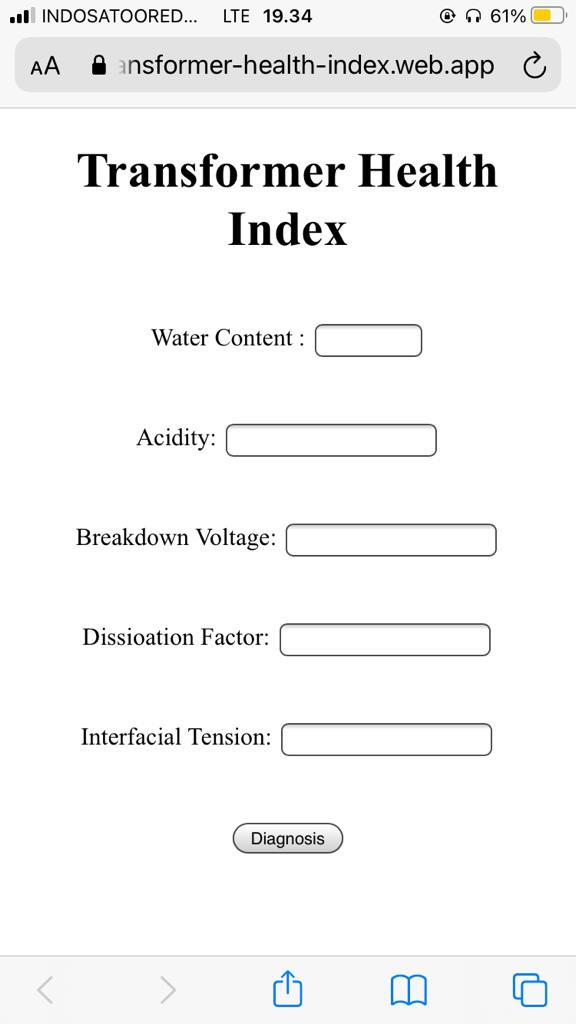
\includegraphics[width=0.4\textwidth]{BAB-4/image/mobile_awal.jpeg}}		
		\captionof{figure}{Tampilan Aplikasi Diagnosis Indeks Kesehatan Transformator Daya pada Perangkat \textit{Mobile}}
		\label{gambar:halaman awal mobile}
\end{minipage}}

Pada proses \textit{input}, masukan data yang diperlukan, pengguna diharuskan untuk mengisi semua kolom yang diperlukan, jika tidak, maka akan muncul peringatan yang menunjukkan data yang dimasukkan kurang. Tampilan peringatan kesalahan dalam mamasukkan data dapat dilihat pada Gambar \ref{gambar:kesalahan input}. Namun, apabila jika pada kondisi pada salah satu masukkan tidak dilakukan pengujian, maka pengguna tetap dapat melakukan diagnosis dengan memasukkan nilai 0. Dengan metode tersebut maka akan meminimalisasi adanya data yang kosong pada saat mendiagnosis indeks kesehatan transformator daya.

\centerline{\begin{minipage}{\linewidth}
		\centering
		\vspace{12 pt}
		%		\input{BAB-4/image/WebAppTA.png}
		\fbox{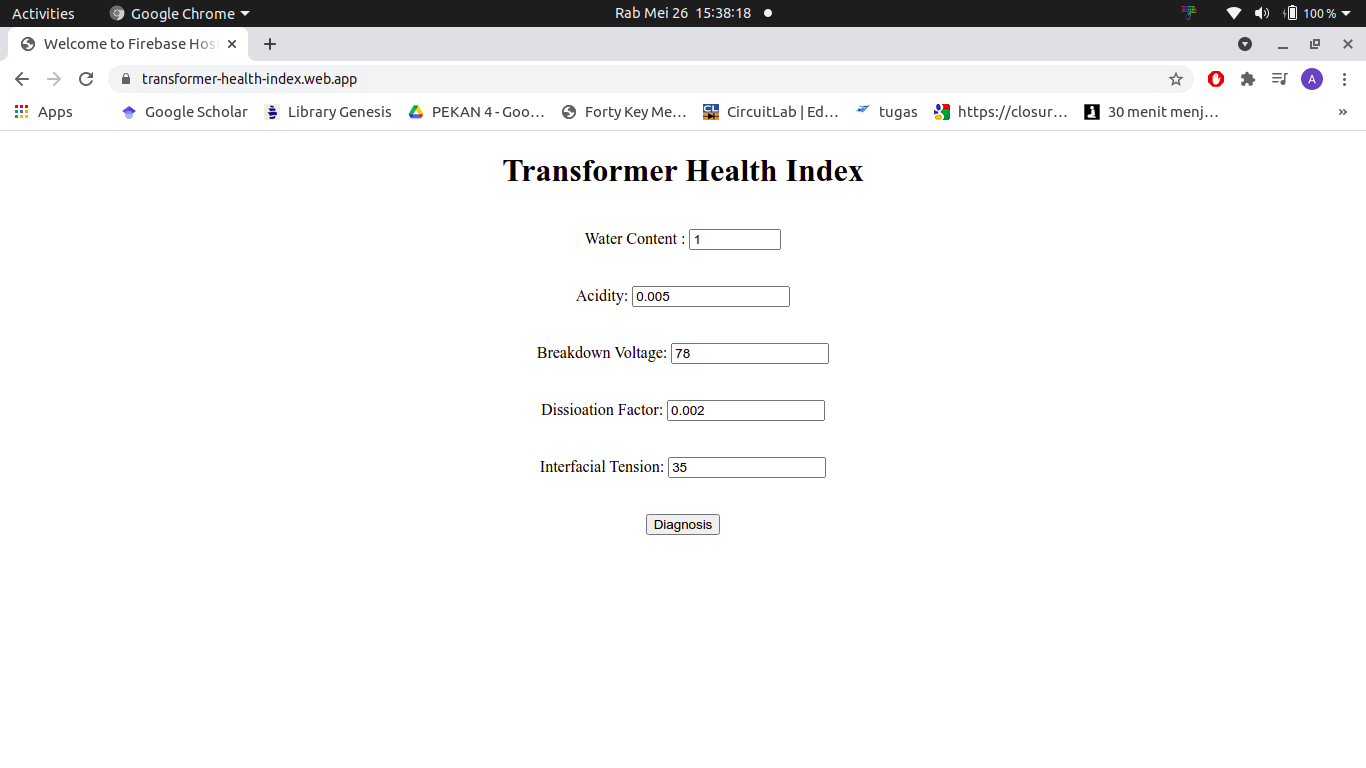
\includegraphics[width=\textwidth]{BAB-4/image/dekstop_view.png}}		
		\captionof{figure}{Tampilan Aplikasi Diagnosis Indeks Kesehatan Transformator Daya pada Perangkat \textit{Dekstop}}
		\label{gambar:halaman awal dekstop}
\end{minipage}}

\centerline{\begin{minipage}{\linewidth}
		\centering
		\vspace{12 pt}
		%		\input{BAB-4/image/WebAppTA.png}
		\fbox{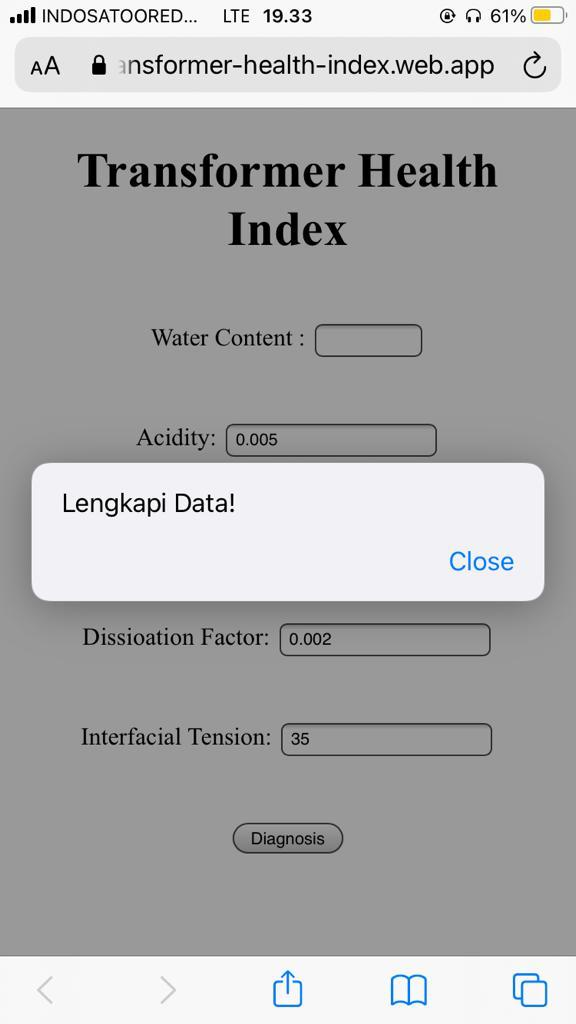
\includegraphics[width=0.4\textwidth]{BAB-4/image/lengkapi_data.jpeg}}		
		\captionof{figure}{Peringatan Aplikasi Jika Terdapat Masukkan yang Belum Lengkap pada Perangkat \textit{Mobile}}
		\label{gambar:kesalahan input}
\end{minipage}}
Kemudian Apabila semua \textit{input} yang diperlukan telah lengkap, pengguna dapat melakukan diagnosis indeks kesehatan transformator daya dengan menekan tombol "Diagnosis", maka hasil diagnosis akan ditampilkan seperti pada Gambar \ref{gambar:berhasil}.

\centerline{\begin{minipage}{\linewidth}
		\centering
		\vspace{12 pt}
		%		\input{BAB-4/image/WebAppTA.png}
		\fbox{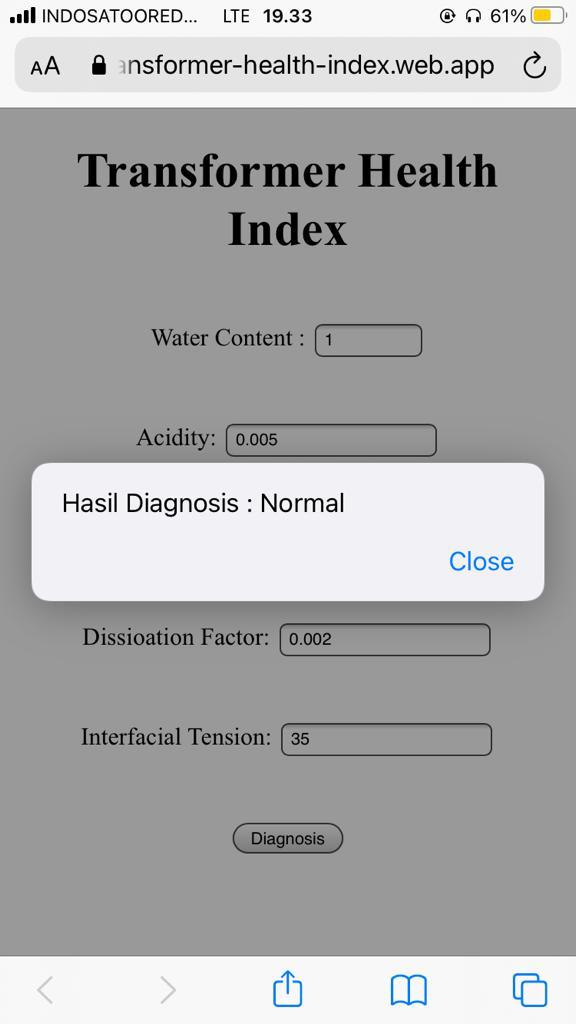
\includegraphics[width=0.4\textwidth]{BAB-4/image/berhasil.jpeg}}		
		\captionof{figure}{Berhasil Mendiagnosis Indeks Kesehatan Transformator Daya pada Perangkat \textit{Mobile}}
		\label{gambar:berhasil}
\end{minipage}}

 
